\chapter{Application on race driving}
This chapter presents the application of the previously developed RLMPC to race driving. First, two car model formulations are presented which approximate real car dynamics with different accuracies. Then, the RLMPC formulation and cost function are introduced and simulations are performed to verify the controller performance.

\section{Race driving}
In general, the goal of race driving is to drive through a given racetrack with the lowest possible lap time. While in real world race driving usually multiple cars are involved, we simplify this problem by assuming only a single car. Mathematically, this can be represented by an optimization problem which minimizes the lap time, given a mathematical model of the car and certain constraints (e.g. lane boundaries, maximum acceleration, and steering angle). Depending on the complexity of the model and the length and shape of the track this can result in a highly complex optimization problem.
%\begin{itemize}
%\item Mathematical: Minimum time problem
%\item Lane constraints
%\item Physical: acceleration, deceleration, corner cutting, no slipping
%\item Friction circle
%\item First assume "real" car, not the BARC model
%\item One or multiple cars -> obstacle avoidance
%\end{itemize}

\section{Car model formulations}
There are many ways to model the dynamics of a car. There are simple models with few states which approximate real car dynamics for low speeds. More sophisticated models with a great number of states can account for slipping conditions (longitudinal and lateral) and effects of tire suspensions.

This thesis presents two basic models, the \emph{kinematic bicycle model} and the \emph{dynamic bicycle model}. Both assume a two-tire bicycle model in which the two front and rear tires of a real car are combined to one front and one rear tire. Furthermore, the former model assumes that the tires can not slip laterally whereas the latter allows for lateral movements of the tires.

Additionally, two coordinate frames are introduced. The first is an inertial x-y-frame, the second is a track-based frame that uses coordinates relative to the race track.

\subsection{Kinematic bicycle model}
The kinematic bicycle model has been adapted from \cite{rajamani2005vehicle}. It is based on the no-slip condition which means that the velocity vectors at both wheels are directed in the orientation of their respective wheel.
Figure \ref{fig:kinModel} shows a standard kinematic bicycle.
\begin{figure}[ht]
	\centering
  	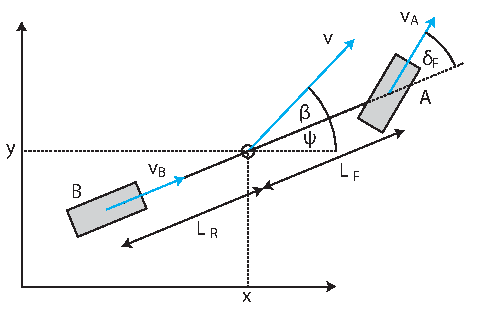
\includegraphics{../../Figures/Models/KinModel.pdf}
	\caption{Kinematic bicycle model}
	\label{fig:kinModel}
\end{figure}
The states in the inertial x-y-frame are the coordinates $x$ and $y$ of the center of the car, the heading angle $\psi$ and the velocity $v$ of the car center. Note that the car center does not necessarily need to coincide with the car's center of gravity since this is a pure geometrical representation of the car model which does not involve masses or forces.\\
The state dynamics can be written as
\begin{align}
\begin{split}
    \dot x &= v \cdot \cos (\psi + \beta)\\
    \dot y &= v \cdot \sin (\psi + \beta)\\
    \dot \psi &= \frac{v}{L_R}\cdot\sin(\beta)\\
    \dot v &= a
\end{split}
\end{align}
with the car's slip angle
\begin{equation}
    \beta = \arctan\left(\frac{L_R}{L_F+L_R}\cdot \tan(\delta_F)\right).
\end{equation}
The control inputs are the longitudinal acceleration $a$ and the steering angle $\delta_F$ at the front wheel.\\
The kinematic bicycle approximates real car dynamics well for low velocities and as long as there is no or only very little tire slip. However, especially for slippery road conditions and higher velocities, model mismatch increases to such an extent that it can not be used to reliably predict real car dynamics anymore. This is why the \emph{dynamic bicycle model} is introduced in the next section.

\subsection{Dynamic bicycle model}
While the kinematic bicycle model is derived geometrically, the dynamic bicycle model is based on forces that occur between the tires and the road. Its states are the longitudinal and lateral velocity $v_x$ and $v_y$ in a body fixed frame, and the yaw rate $\dot \psi$. The corresponding model is illustrated in Fig. \ref{fig:dynModel}. The state dynamics presented in eq. \eqref{eq:dynModel} can be derived by applying Newton's second law of motion \cite{Kong2015}:
\begin{align}
\begin{split}
\label{eq:dynModel}
    \dot v_x &= a+\dot \psi\cdot v_y\\
    \dot v_y &= \frac{1}{m}\cdot (F_F\cdot \cos(\delta_F)+F_R)-\dot\psi\cdot v_x\\
    \ddot \psi &= \frac{1}{I_Z}\cdot(L_F\cdot F_F - L_R\cdot F_R)
\end{split}
\end{align}
These state dynamics assume that there is only lateral but no longitudinal tire slip which might occur during high accelerations or decelerations. We can avoid longitudinal tire slip by constraining the acceleration input $a$ to small values. This allows us to neglect this effect in the model formulation.
\begin{figure}[ht]
	\centering
  	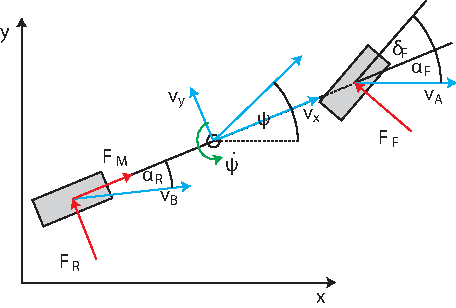
\includegraphics{../../Figures/Models/DynModel.pdf}
	\caption{Dynamic bicycle model}
	\label{fig:dynModel}
\end{figure}
The tire forces $F_F$ and $F_R$ depend on the lateral slipping angles $\alpha_F$ and $\alpha_R$ of the front and the rear tire, respectively. One common function that approximates the tire forces is the \emph{Pacejka} function from \cite{pacejka1987} (often referred to as \emph{Magic formula}):
% REFERENCE
\begin{equation}\label{eq:pacejka}
f_P(\alpha) = D\cdot\sin(C\cdot\arctan(B\cdot\alpha))
\end{equation}
\emph{Note:} Eq. \eqref{eq:pacejka} is a simplified version of the more general Pacejka function.\\
The Pacejka function is illustrated in Fig. \ref{fig:Pacejka} for two sets of parameters, one for tire forces on a dry road and one for a snowy road. The chosen values are not parameters of a real tire, they are only meant for illustration purposes. We can see in this figure that the lateral tire force reaches a peak at a specific slip angle before it decreases, leading to the effect commonly known as drifting.
\begin{table}[h!]
\centering
\caption{Pacejka coefficients for different road conditions}
\begin{tabular}{l|l|l|l}
Parameter & Meaning & Dry & Snowy\\
\hline
B & Stiffness factor & 10 & 5\\
C & Shape factor & 1.9 & 2\\
D & Peak factor & 1 & 0.3
\end{tabular}
\label{tab:pacejka}
\end{table}

\begin{figure}[ht]
	\centering
  	%% Creator: Matplotlib, PGF backend
%%
%% To include the figure in your LaTeX document, write
%%   \input{<filename>.pgf}
%%
%% Make sure the required packages are loaded in your preamble
%%   \usepackage{pgf}
%%
%% Figures using additional raster images can only be included by \input if
%% they are in the same directory as the main LaTeX file. For loading figures
%% from other directories you can use the `import` package
%%   \usepackage{import}
%% and then include the figures with
%%   \import{<path to file>}{<filename>.pgf}
%%
%% Matplotlib used the following preamble
%%   \usepackage{fontspec}
%%
\begingroup%
\makeatletter%
\begin{pgfpicture}%
\pgfpathrectangle{\pgfpointorigin}{\pgfqpoint{5.000000in}{3.000000in}}%
\pgfusepath{use as bounding box, clip}%
\begin{pgfscope}%
\pgfsetbuttcap%
\pgfsetmiterjoin%
\definecolor{currentfill}{rgb}{1.000000,1.000000,1.000000}%
\pgfsetfillcolor{currentfill}%
\pgfsetlinewidth{0.000000pt}%
\definecolor{currentstroke}{rgb}{1.000000,1.000000,1.000000}%
\pgfsetstrokecolor{currentstroke}%
\pgfsetdash{}{0pt}%
\pgfpathmoveto{\pgfqpoint{0.000000in}{0.000000in}}%
\pgfpathlineto{\pgfqpoint{5.000000in}{0.000000in}}%
\pgfpathlineto{\pgfqpoint{5.000000in}{3.000000in}}%
\pgfpathlineto{\pgfqpoint{0.000000in}{3.000000in}}%
\pgfpathclose%
\pgfusepath{fill}%
\end{pgfscope}%
\begin{pgfscope}%
\pgfsetbuttcap%
\pgfsetmiterjoin%
\definecolor{currentfill}{rgb}{1.000000,1.000000,1.000000}%
\pgfsetfillcolor{currentfill}%
\pgfsetlinewidth{0.000000pt}%
\definecolor{currentstroke}{rgb}{0.000000,0.000000,0.000000}%
\pgfsetstrokecolor{currentstroke}%
\pgfsetstrokeopacity{0.000000}%
\pgfsetdash{}{0pt}%
\pgfpathmoveto{\pgfqpoint{0.636556in}{0.471921in}}%
\pgfpathlineto{\pgfqpoint{4.791316in}{0.471921in}}%
\pgfpathlineto{\pgfqpoint{4.791316in}{2.850000in}}%
\pgfpathlineto{\pgfqpoint{0.636556in}{2.850000in}}%
\pgfpathclose%
\pgfusepath{fill}%
\end{pgfscope}%
\begin{pgfscope}%
\pgfpathrectangle{\pgfqpoint{0.636556in}{0.471921in}}{\pgfqpoint{4.154761in}{2.378079in}} %
\pgfusepath{clip}%
\pgfsetrectcap%
\pgfsetroundjoin%
\pgfsetlinewidth{0.501875pt}%
\definecolor{currentstroke}{rgb}{0.000000,0.000000,1.000000}%
\pgfsetstrokecolor{currentstroke}%
\pgfsetdash{}{0pt}%
\pgfpathmoveto{\pgfqpoint{0.636556in}{1.127960in}}%
\pgfpathlineto{\pgfqpoint{0.676231in}{1.121567in}}%
\pgfpathlineto{\pgfqpoint{0.715906in}{1.114955in}}%
\pgfpathlineto{\pgfqpoint{0.755581in}{1.108115in}}%
\pgfpathlineto{\pgfqpoint{0.795256in}{1.101035in}}%
\pgfpathlineto{\pgfqpoint{0.834931in}{1.093703in}}%
\pgfpathlineto{\pgfqpoint{0.874606in}{1.086107in}}%
\pgfpathlineto{\pgfqpoint{0.914281in}{1.078233in}}%
\pgfpathlineto{\pgfqpoint{0.953956in}{1.070067in}}%
\pgfpathlineto{\pgfqpoint{0.993631in}{1.061594in}}%
\pgfpathlineto{\pgfqpoint{1.033306in}{1.052798in}}%
\pgfpathlineto{\pgfqpoint{1.072981in}{1.043662in}}%
\pgfpathlineto{\pgfqpoint{1.112656in}{1.034169in}}%
\pgfpathlineto{\pgfqpoint{1.152331in}{1.024300in}}%
\pgfpathlineto{\pgfqpoint{1.192006in}{1.014034in}}%
\pgfpathlineto{\pgfqpoint{1.231681in}{1.003352in}}%
\pgfpathlineto{\pgfqpoint{1.271356in}{0.992232in}}%
\pgfpathlineto{\pgfqpoint{1.311031in}{0.980650in}}%
\pgfpathlineto{\pgfqpoint{1.350706in}{0.968585in}}%
\pgfpathlineto{\pgfqpoint{1.390381in}{0.956010in}}%
\pgfpathlineto{\pgfqpoint{1.430056in}{0.942903in}}%
\pgfpathlineto{\pgfqpoint{1.469732in}{0.929238in}}%
\pgfpathlineto{\pgfqpoint{1.509407in}{0.914989in}}%
\pgfpathlineto{\pgfqpoint{1.549082in}{0.900135in}}%
\pgfpathlineto{\pgfqpoint{1.588757in}{0.884652in}}%
\pgfpathlineto{\pgfqpoint{1.628432in}{0.868520in}}%
\pgfpathlineto{\pgfqpoint{1.668107in}{0.851725in}}%
\pgfpathlineto{\pgfqpoint{1.707782in}{0.834257in}}%
\pgfpathlineto{\pgfqpoint{1.747457in}{0.816115in}}%
\pgfpathlineto{\pgfqpoint{1.787132in}{0.797310in}}%
\pgfpathlineto{\pgfqpoint{1.826807in}{0.777871in}}%
\pgfpathlineto{\pgfqpoint{1.866482in}{0.757849in}}%
\pgfpathlineto{\pgfqpoint{1.906157in}{0.737326in}}%
\pgfpathlineto{\pgfqpoint{1.945832in}{0.716426in}}%
\pgfpathlineto{\pgfqpoint{1.985507in}{0.695329in}}%
\pgfpathlineto{\pgfqpoint{2.025182in}{0.674291in}}%
\pgfpathlineto{\pgfqpoint{2.064857in}{0.653666in}}%
\pgfpathlineto{\pgfqpoint{2.104532in}{0.633943in}}%
\pgfpathlineto{\pgfqpoint{2.144207in}{0.615780in}}%
\pgfpathlineto{\pgfqpoint{2.183882in}{0.600060in}}%
\pgfpathlineto{\pgfqpoint{2.223557in}{0.587951in}}%
\pgfpathlineto{\pgfqpoint{2.263232in}{0.580981in}}%
\pgfpathlineto{\pgfqpoint{2.302907in}{0.581108in}}%
\pgfpathlineto{\pgfqpoint{2.342582in}{0.590794in}}%
\pgfpathlineto{\pgfqpoint{2.382258in}{0.613039in}}%
\pgfpathlineto{\pgfqpoint{2.421933in}{0.651339in}}%
\pgfpathlineto{\pgfqpoint{2.461608in}{0.709516in}}%
\pgfpathlineto{\pgfqpoint{2.501283in}{0.791335in}}%
\pgfpathlineto{\pgfqpoint{2.540958in}{0.899858in}}%
\pgfpathlineto{\pgfqpoint{2.580633in}{1.036540in}}%
\pgfpathlineto{\pgfqpoint{2.620308in}{1.200230in}}%
\pgfpathlineto{\pgfqpoint{2.659983in}{1.386413in}}%
\pgfpathlineto{\pgfqpoint{2.699658in}{1.587138in}}%
\pgfpathlineto{\pgfqpoint{2.739333in}{1.791927in}}%
\pgfpathlineto{\pgfqpoint{2.779008in}{1.989552in}}%
\pgfpathlineto{\pgfqpoint{2.818683in}{2.170094in}}%
\pgfpathlineto{\pgfqpoint{2.858358in}{2.326517in}}%
\pgfpathlineto{\pgfqpoint{2.898033in}{2.455293in}}%
\pgfpathlineto{\pgfqpoint{2.937708in}{2.556098in}}%
\pgfpathlineto{\pgfqpoint{2.977383in}{2.630938in}}%
\pgfpathlineto{\pgfqpoint{3.017058in}{2.683152in}}%
\pgfpathlineto{\pgfqpoint{3.056733in}{2.716576in}}%
\pgfpathlineto{\pgfqpoint{3.096408in}{2.734969in}}%
\pgfpathlineto{\pgfqpoint{3.136083in}{2.741697in}}%
\pgfpathlineto{\pgfqpoint{3.175758in}{2.739610in}}%
\pgfpathlineto{\pgfqpoint{3.215433in}{2.731021in}}%
\pgfpathlineto{\pgfqpoint{3.255108in}{2.717764in}}%
\pgfpathlineto{\pgfqpoint{3.294784in}{2.701254in}}%
\pgfpathlineto{\pgfqpoint{3.334459in}{2.682576in}}%
\pgfpathlineto{\pgfqpoint{3.374134in}{2.662542in}}%
\pgfpathlineto{\pgfqpoint{3.413809in}{2.641759in}}%
\pgfpathlineto{\pgfqpoint{3.453484in}{2.620673in}}%
\pgfpathlineto{\pgfqpoint{3.493159in}{2.599609in}}%
\pgfpathlineto{\pgfqpoint{3.532834in}{2.578799in}}%
\pgfpathlineto{\pgfqpoint{3.572509in}{2.558406in}}%
\pgfpathlineto{\pgfqpoint{3.612184in}{2.538540in}}%
\pgfpathlineto{\pgfqpoint{3.651859in}{2.519275in}}%
\pgfpathlineto{\pgfqpoint{3.691534in}{2.500654in}}%
\pgfpathlineto{\pgfqpoint{3.731209in}{2.482700in}}%
\pgfpathlineto{\pgfqpoint{3.770884in}{2.465421in}}%
\pgfpathlineto{\pgfqpoint{3.810559in}{2.448813in}}%
\pgfpathlineto{\pgfqpoint{3.850234in}{2.432865in}}%
\pgfpathlineto{\pgfqpoint{3.889909in}{2.417561in}}%
\pgfpathlineto{\pgfqpoint{3.929584in}{2.402878in}}%
\pgfpathlineto{\pgfqpoint{3.969259in}{2.388796in}}%
\pgfpathlineto{\pgfqpoint{4.008934in}{2.375289in}}%
\pgfpathlineto{\pgfqpoint{4.048609in}{2.362334in}}%
\pgfpathlineto{\pgfqpoint{4.088284in}{2.349905in}}%
\pgfpathlineto{\pgfqpoint{4.127959in}{2.337977in}}%
\pgfpathlineto{\pgfqpoint{4.167635in}{2.326527in}}%
\pgfpathlineto{\pgfqpoint{4.207310in}{2.315532in}}%
\pgfpathlineto{\pgfqpoint{4.246985in}{2.304969in}}%
\pgfpathlineto{\pgfqpoint{4.286660in}{2.294816in}}%
\pgfpathlineto{\pgfqpoint{4.326335in}{2.285054in}}%
\pgfpathlineto{\pgfqpoint{4.366010in}{2.275663in}}%
\pgfpathlineto{\pgfqpoint{4.405685in}{2.266624in}}%
\pgfpathlineto{\pgfqpoint{4.445360in}{2.257921in}}%
\pgfpathlineto{\pgfqpoint{4.485035in}{2.249535in}}%
\pgfpathlineto{\pgfqpoint{4.524710in}{2.241453in}}%
\pgfpathlineto{\pgfqpoint{4.564385in}{2.233658in}}%
\pgfpathlineto{\pgfqpoint{4.604060in}{2.226137in}}%
\pgfpathlineto{\pgfqpoint{4.643735in}{2.218877in}}%
\pgfpathlineto{\pgfqpoint{4.683410in}{2.211865in}}%
\pgfpathlineto{\pgfqpoint{4.723085in}{2.205090in}}%
\pgfpathlineto{\pgfqpoint{4.762760in}{2.198541in}}%
\pgfusepath{stroke}%
\end{pgfscope}%
\begin{pgfscope}%
\pgfpathrectangle{\pgfqpoint{0.636556in}{0.471921in}}{\pgfqpoint{4.154761in}{2.378079in}} %
\pgfusepath{clip}%
\pgfsetrectcap%
\pgfsetroundjoin%
\pgfsetlinewidth{0.501875pt}%
\definecolor{currentstroke}{rgb}{0.000000,0.500000,0.000000}%
\pgfsetstrokecolor{currentstroke}%
\pgfsetdash{}{0pt}%
\pgfpathmoveto{\pgfqpoint{0.636556in}{1.444769in}}%
\pgfpathlineto{\pgfqpoint{0.676231in}{1.441658in}}%
\pgfpathlineto{\pgfqpoint{0.715906in}{1.438478in}}%
\pgfpathlineto{\pgfqpoint{0.755581in}{1.435229in}}%
\pgfpathlineto{\pgfqpoint{0.795256in}{1.431911in}}%
\pgfpathlineto{\pgfqpoint{0.834931in}{1.428524in}}%
\pgfpathlineto{\pgfqpoint{0.874606in}{1.425067in}}%
\pgfpathlineto{\pgfqpoint{0.914281in}{1.421541in}}%
\pgfpathlineto{\pgfqpoint{0.953956in}{1.417947in}}%
\pgfpathlineto{\pgfqpoint{0.993631in}{1.414287in}}%
\pgfpathlineto{\pgfqpoint{1.033306in}{1.410562in}}%
\pgfpathlineto{\pgfqpoint{1.072981in}{1.406775in}}%
\pgfpathlineto{\pgfqpoint{1.112656in}{1.402931in}}%
\pgfpathlineto{\pgfqpoint{1.152331in}{1.399032in}}%
\pgfpathlineto{\pgfqpoint{1.192006in}{1.395086in}}%
\pgfpathlineto{\pgfqpoint{1.231681in}{1.391098in}}%
\pgfpathlineto{\pgfqpoint{1.271356in}{1.387078in}}%
\pgfpathlineto{\pgfqpoint{1.311031in}{1.383036in}}%
\pgfpathlineto{\pgfqpoint{1.350706in}{1.378983in}}%
\pgfpathlineto{\pgfqpoint{1.390381in}{1.374935in}}%
\pgfpathlineto{\pgfqpoint{1.430056in}{1.370909in}}%
\pgfpathlineto{\pgfqpoint{1.469732in}{1.366926in}}%
\pgfpathlineto{\pgfqpoint{1.509407in}{1.363010in}}%
\pgfpathlineto{\pgfqpoint{1.549082in}{1.359188in}}%
\pgfpathlineto{\pgfqpoint{1.588757in}{1.355496in}}%
\pgfpathlineto{\pgfqpoint{1.628432in}{1.351971in}}%
\pgfpathlineto{\pgfqpoint{1.668107in}{1.348657in}}%
\pgfpathlineto{\pgfqpoint{1.707782in}{1.345608in}}%
\pgfpathlineto{\pgfqpoint{1.747457in}{1.342882in}}%
\pgfpathlineto{\pgfqpoint{1.787132in}{1.340548in}}%
\pgfpathlineto{\pgfqpoint{1.826807in}{1.338684in}}%
\pgfpathlineto{\pgfqpoint{1.866482in}{1.337377in}}%
\pgfpathlineto{\pgfqpoint{1.906157in}{1.336729in}}%
\pgfpathlineto{\pgfqpoint{1.945832in}{1.336848in}}%
\pgfpathlineto{\pgfqpoint{1.985507in}{1.337860in}}%
\pgfpathlineto{\pgfqpoint{2.025182in}{1.339900in}}%
\pgfpathlineto{\pgfqpoint{2.064857in}{1.343113in}}%
\pgfpathlineto{\pgfqpoint{2.104532in}{1.347656in}}%
\pgfpathlineto{\pgfqpoint{2.144207in}{1.353694in}}%
\pgfpathlineto{\pgfqpoint{2.183882in}{1.361393in}}%
\pgfpathlineto{\pgfqpoint{2.223557in}{1.370921in}}%
\pgfpathlineto{\pgfqpoint{2.263232in}{1.382435in}}%
\pgfpathlineto{\pgfqpoint{2.302907in}{1.396079in}}%
\pgfpathlineto{\pgfqpoint{2.342582in}{1.411969in}}%
\pgfpathlineto{\pgfqpoint{2.382258in}{1.430184in}}%
\pgfpathlineto{\pgfqpoint{2.421933in}{1.450757in}}%
\pgfpathlineto{\pgfqpoint{2.461608in}{1.473660in}}%
\pgfpathlineto{\pgfqpoint{2.501283in}{1.498795in}}%
\pgfpathlineto{\pgfqpoint{2.540958in}{1.525991in}}%
\pgfpathlineto{\pgfqpoint{2.580633in}{1.554996in}}%
\pgfpathlineto{\pgfqpoint{2.620308in}{1.585484in}}%
\pgfpathlineto{\pgfqpoint{2.659983in}{1.617065in}}%
\pgfpathlineto{\pgfqpoint{2.699658in}{1.649294in}}%
\pgfpathlineto{\pgfqpoint{2.739333in}{1.681697in}}%
\pgfpathlineto{\pgfqpoint{2.779008in}{1.713792in}}%
\pgfpathlineto{\pgfqpoint{2.818683in}{1.745109in}}%
\pgfpathlineto{\pgfqpoint{2.858358in}{1.775219in}}%
\pgfpathlineto{\pgfqpoint{2.898033in}{1.803746in}}%
\pgfpathlineto{\pgfqpoint{2.937708in}{1.830386in}}%
\pgfpathlineto{\pgfqpoint{2.977383in}{1.854910in}}%
\pgfpathlineto{\pgfqpoint{3.017058in}{1.877166in}}%
\pgfpathlineto{\pgfqpoint{3.056733in}{1.897079in}}%
\pgfpathlineto{\pgfqpoint{3.096408in}{1.914637in}}%
\pgfpathlineto{\pgfqpoint{3.136083in}{1.929888in}}%
\pgfpathlineto{\pgfqpoint{3.175758in}{1.942921in}}%
\pgfpathlineto{\pgfqpoint{3.215433in}{1.953864in}}%
\pgfpathlineto{\pgfqpoint{3.255108in}{1.962863in}}%
\pgfpathlineto{\pgfqpoint{3.294784in}{1.970079in}}%
\pgfpathlineto{\pgfqpoint{3.334459in}{1.975681in}}%
\pgfpathlineto{\pgfqpoint{3.374134in}{1.979836in}}%
\pgfpathlineto{\pgfqpoint{3.413809in}{1.982705in}}%
\pgfpathlineto{\pgfqpoint{3.453484in}{1.984442in}}%
\pgfpathlineto{\pgfqpoint{3.493159in}{1.985191in}}%
\pgfpathlineto{\pgfqpoint{3.532834in}{1.985083in}}%
\pgfpathlineto{\pgfqpoint{3.572509in}{1.984239in}}%
\pgfpathlineto{\pgfqpoint{3.612184in}{1.982767in}}%
\pgfpathlineto{\pgfqpoint{3.651859in}{1.980763in}}%
\pgfpathlineto{\pgfqpoint{3.691534in}{1.978311in}}%
\pgfpathlineto{\pgfqpoint{3.731209in}{1.975488in}}%
\pgfpathlineto{\pgfqpoint{3.770884in}{1.972359in}}%
\pgfpathlineto{\pgfqpoint{3.810559in}{1.968982in}}%
\pgfpathlineto{\pgfqpoint{3.850234in}{1.965405in}}%
\pgfpathlineto{\pgfqpoint{3.889909in}{1.961673in}}%
\pgfpathlineto{\pgfqpoint{3.929584in}{1.957822in}}%
\pgfpathlineto{\pgfqpoint{3.969259in}{1.953884in}}%
\pgfpathlineto{\pgfqpoint{4.008934in}{1.949887in}}%
\pgfpathlineto{\pgfqpoint{4.048609in}{1.945853in}}%
\pgfpathlineto{\pgfqpoint{4.088284in}{1.941802in}}%
\pgfpathlineto{\pgfqpoint{4.127959in}{1.937751in}}%
\pgfpathlineto{\pgfqpoint{4.167635in}{1.933713in}}%
\pgfpathlineto{\pgfqpoint{4.207310in}{1.929701in}}%
\pgfpathlineto{\pgfqpoint{4.246985in}{1.925725in}}%
\pgfpathlineto{\pgfqpoint{4.286660in}{1.921791in}}%
\pgfpathlineto{\pgfqpoint{4.326335in}{1.917907in}}%
\pgfpathlineto{\pgfqpoint{4.366010in}{1.914078in}}%
\pgfpathlineto{\pgfqpoint{4.405685in}{1.910309in}}%
\pgfpathlineto{\pgfqpoint{4.445360in}{1.906602in}}%
\pgfpathlineto{\pgfqpoint{4.485035in}{1.902960in}}%
\pgfpathlineto{\pgfqpoint{4.524710in}{1.899385in}}%
\pgfpathlineto{\pgfqpoint{4.564385in}{1.895879in}}%
\pgfpathlineto{\pgfqpoint{4.604060in}{1.892441in}}%
\pgfpathlineto{\pgfqpoint{4.643735in}{1.889073in}}%
\pgfpathlineto{\pgfqpoint{4.683410in}{1.885774in}}%
\pgfpathlineto{\pgfqpoint{4.723085in}{1.882545in}}%
\pgfpathlineto{\pgfqpoint{4.762760in}{1.879385in}}%
\pgfusepath{stroke}%
\end{pgfscope}%
\begin{pgfscope}%
\pgfsetrectcap%
\pgfsetmiterjoin%
\pgfsetlinewidth{0.501875pt}%
\definecolor{currentstroke}{rgb}{0.000000,0.000000,0.000000}%
\pgfsetstrokecolor{currentstroke}%
\pgfsetdash{}{0pt}%
\pgfpathmoveto{\pgfqpoint{0.636556in}{2.850000in}}%
\pgfpathlineto{\pgfqpoint{4.791316in}{2.850000in}}%
\pgfusepath{stroke}%
\end{pgfscope}%
\begin{pgfscope}%
\pgfsetrectcap%
\pgfsetmiterjoin%
\pgfsetlinewidth{0.501875pt}%
\definecolor{currentstroke}{rgb}{0.000000,0.000000,0.000000}%
\pgfsetstrokecolor{currentstroke}%
\pgfsetdash{}{0pt}%
\pgfpathmoveto{\pgfqpoint{4.791316in}{0.471921in}}%
\pgfpathlineto{\pgfqpoint{4.791316in}{2.850000in}}%
\pgfusepath{stroke}%
\end{pgfscope}%
\begin{pgfscope}%
\pgfsetrectcap%
\pgfsetmiterjoin%
\pgfsetlinewidth{0.501875pt}%
\definecolor{currentstroke}{rgb}{0.000000,0.000000,0.000000}%
\pgfsetstrokecolor{currentstroke}%
\pgfsetdash{}{0pt}%
\pgfpathmoveto{\pgfqpoint{0.636556in}{0.471921in}}%
\pgfpathlineto{\pgfqpoint{4.791316in}{0.471921in}}%
\pgfusepath{stroke}%
\end{pgfscope}%
\begin{pgfscope}%
\pgfsetrectcap%
\pgfsetmiterjoin%
\pgfsetlinewidth{0.501875pt}%
\definecolor{currentstroke}{rgb}{0.000000,0.000000,0.000000}%
\pgfsetstrokecolor{currentstroke}%
\pgfsetdash{}{0pt}%
\pgfpathmoveto{\pgfqpoint{0.636556in}{0.471921in}}%
\pgfpathlineto{\pgfqpoint{0.636556in}{2.850000in}}%
\pgfusepath{stroke}%
\end{pgfscope}%
\begin{pgfscope}%
\pgfpathrectangle{\pgfqpoint{0.636556in}{0.471921in}}{\pgfqpoint{4.154761in}{2.378079in}} %
\pgfusepath{clip}%
\pgfsetbuttcap%
\pgfsetroundjoin%
\pgfsetlinewidth{0.501875pt}%
\definecolor{currentstroke}{rgb}{0.000000,0.000000,0.000000}%
\pgfsetstrokecolor{currentstroke}%
\pgfsetdash{{1.000000pt}{3.000000pt}}{0.000000pt}%
\pgfpathmoveto{\pgfqpoint{0.636556in}{0.471921in}}%
\pgfpathlineto{\pgfqpoint{0.636556in}{2.850000in}}%
\pgfusepath{stroke}%
\end{pgfscope}%
\begin{pgfscope}%
\pgfsetbuttcap%
\pgfsetroundjoin%
\definecolor{currentfill}{rgb}{0.000000,0.000000,0.000000}%
\pgfsetfillcolor{currentfill}%
\pgfsetlinewidth{0.250937pt}%
\definecolor{currentstroke}{rgb}{0.000000,0.000000,0.000000}%
\pgfsetstrokecolor{currentstroke}%
\pgfsetdash{}{0pt}%
\pgfsys@defobject{currentmarker}{\pgfqpoint{0.000000in}{0.000000in}}{\pgfqpoint{0.000000in}{0.055556in}}{%
\pgfpathmoveto{\pgfqpoint{0.000000in}{0.000000in}}%
\pgfpathlineto{\pgfqpoint{0.000000in}{0.055556in}}%
\pgfusepath{stroke,fill}%
}%
\begin{pgfscope}%
\pgfsys@transformshift{0.636556in}{0.471921in}%
\pgfsys@useobject{currentmarker}{}%
\end{pgfscope}%
\end{pgfscope}%
\begin{pgfscope}%
\pgfsetbuttcap%
\pgfsetroundjoin%
\definecolor{currentfill}{rgb}{0.000000,0.000000,0.000000}%
\pgfsetfillcolor{currentfill}%
\pgfsetlinewidth{0.250937pt}%
\definecolor{currentstroke}{rgb}{0.000000,0.000000,0.000000}%
\pgfsetstrokecolor{currentstroke}%
\pgfsetdash{}{0pt}%
\pgfsys@defobject{currentmarker}{\pgfqpoint{0.000000in}{-0.055556in}}{\pgfqpoint{0.000000in}{0.000000in}}{%
\pgfpathmoveto{\pgfqpoint{0.000000in}{0.000000in}}%
\pgfpathlineto{\pgfqpoint{0.000000in}{-0.055556in}}%
\pgfusepath{stroke,fill}%
}%
\begin{pgfscope}%
\pgfsys@transformshift{0.636556in}{2.850000in}%
\pgfsys@useobject{currentmarker}{}%
\end{pgfscope}%
\end{pgfscope}%
\begin{pgfscope}%
\pgftext[x=0.636556in,y=0.416365in,,top]{\rmfamily\fontsize{6.940000}{8.328000}\selectfont \(\displaystyle -30\)}%
\end{pgfscope}%
\begin{pgfscope}%
\pgfpathrectangle{\pgfqpoint{0.636556in}{0.471921in}}{\pgfqpoint{4.154761in}{2.378079in}} %
\pgfusepath{clip}%
\pgfsetbuttcap%
\pgfsetroundjoin%
\pgfsetlinewidth{0.501875pt}%
\definecolor{currentstroke}{rgb}{0.000000,0.000000,0.000000}%
\pgfsetstrokecolor{currentstroke}%
\pgfsetdash{{1.000000pt}{3.000000pt}}{0.000000pt}%
\pgfpathmoveto{\pgfqpoint{1.329016in}{0.471921in}}%
\pgfpathlineto{\pgfqpoint{1.329016in}{2.850000in}}%
\pgfusepath{stroke}%
\end{pgfscope}%
\begin{pgfscope}%
\pgfsetbuttcap%
\pgfsetroundjoin%
\definecolor{currentfill}{rgb}{0.000000,0.000000,0.000000}%
\pgfsetfillcolor{currentfill}%
\pgfsetlinewidth{0.250937pt}%
\definecolor{currentstroke}{rgb}{0.000000,0.000000,0.000000}%
\pgfsetstrokecolor{currentstroke}%
\pgfsetdash{}{0pt}%
\pgfsys@defobject{currentmarker}{\pgfqpoint{0.000000in}{0.000000in}}{\pgfqpoint{0.000000in}{0.055556in}}{%
\pgfpathmoveto{\pgfqpoint{0.000000in}{0.000000in}}%
\pgfpathlineto{\pgfqpoint{0.000000in}{0.055556in}}%
\pgfusepath{stroke,fill}%
}%
\begin{pgfscope}%
\pgfsys@transformshift{1.329016in}{0.471921in}%
\pgfsys@useobject{currentmarker}{}%
\end{pgfscope}%
\end{pgfscope}%
\begin{pgfscope}%
\pgfsetbuttcap%
\pgfsetroundjoin%
\definecolor{currentfill}{rgb}{0.000000,0.000000,0.000000}%
\pgfsetfillcolor{currentfill}%
\pgfsetlinewidth{0.250937pt}%
\definecolor{currentstroke}{rgb}{0.000000,0.000000,0.000000}%
\pgfsetstrokecolor{currentstroke}%
\pgfsetdash{}{0pt}%
\pgfsys@defobject{currentmarker}{\pgfqpoint{0.000000in}{-0.055556in}}{\pgfqpoint{0.000000in}{0.000000in}}{%
\pgfpathmoveto{\pgfqpoint{0.000000in}{0.000000in}}%
\pgfpathlineto{\pgfqpoint{0.000000in}{-0.055556in}}%
\pgfusepath{stroke,fill}%
}%
\begin{pgfscope}%
\pgfsys@transformshift{1.329016in}{2.850000in}%
\pgfsys@useobject{currentmarker}{}%
\end{pgfscope}%
\end{pgfscope}%
\begin{pgfscope}%
\pgftext[x=1.329016in,y=0.416365in,,top]{\rmfamily\fontsize{6.940000}{8.328000}\selectfont \(\displaystyle -20\)}%
\end{pgfscope}%
\begin{pgfscope}%
\pgfpathrectangle{\pgfqpoint{0.636556in}{0.471921in}}{\pgfqpoint{4.154761in}{2.378079in}} %
\pgfusepath{clip}%
\pgfsetbuttcap%
\pgfsetroundjoin%
\pgfsetlinewidth{0.501875pt}%
\definecolor{currentstroke}{rgb}{0.000000,0.000000,0.000000}%
\pgfsetstrokecolor{currentstroke}%
\pgfsetdash{{1.000000pt}{3.000000pt}}{0.000000pt}%
\pgfpathmoveto{\pgfqpoint{2.021476in}{0.471921in}}%
\pgfpathlineto{\pgfqpoint{2.021476in}{2.850000in}}%
\pgfusepath{stroke}%
\end{pgfscope}%
\begin{pgfscope}%
\pgfsetbuttcap%
\pgfsetroundjoin%
\definecolor{currentfill}{rgb}{0.000000,0.000000,0.000000}%
\pgfsetfillcolor{currentfill}%
\pgfsetlinewidth{0.250937pt}%
\definecolor{currentstroke}{rgb}{0.000000,0.000000,0.000000}%
\pgfsetstrokecolor{currentstroke}%
\pgfsetdash{}{0pt}%
\pgfsys@defobject{currentmarker}{\pgfqpoint{0.000000in}{0.000000in}}{\pgfqpoint{0.000000in}{0.055556in}}{%
\pgfpathmoveto{\pgfqpoint{0.000000in}{0.000000in}}%
\pgfpathlineto{\pgfqpoint{0.000000in}{0.055556in}}%
\pgfusepath{stroke,fill}%
}%
\begin{pgfscope}%
\pgfsys@transformshift{2.021476in}{0.471921in}%
\pgfsys@useobject{currentmarker}{}%
\end{pgfscope}%
\end{pgfscope}%
\begin{pgfscope}%
\pgfsetbuttcap%
\pgfsetroundjoin%
\definecolor{currentfill}{rgb}{0.000000,0.000000,0.000000}%
\pgfsetfillcolor{currentfill}%
\pgfsetlinewidth{0.250937pt}%
\definecolor{currentstroke}{rgb}{0.000000,0.000000,0.000000}%
\pgfsetstrokecolor{currentstroke}%
\pgfsetdash{}{0pt}%
\pgfsys@defobject{currentmarker}{\pgfqpoint{0.000000in}{-0.055556in}}{\pgfqpoint{0.000000in}{0.000000in}}{%
\pgfpathmoveto{\pgfqpoint{0.000000in}{0.000000in}}%
\pgfpathlineto{\pgfqpoint{0.000000in}{-0.055556in}}%
\pgfusepath{stroke,fill}%
}%
\begin{pgfscope}%
\pgfsys@transformshift{2.021476in}{2.850000in}%
\pgfsys@useobject{currentmarker}{}%
\end{pgfscope}%
\end{pgfscope}%
\begin{pgfscope}%
\pgftext[x=2.021476in,y=0.416365in,,top]{\rmfamily\fontsize{6.940000}{8.328000}\selectfont \(\displaystyle -10\)}%
\end{pgfscope}%
\begin{pgfscope}%
\pgfpathrectangle{\pgfqpoint{0.636556in}{0.471921in}}{\pgfqpoint{4.154761in}{2.378079in}} %
\pgfusepath{clip}%
\pgfsetbuttcap%
\pgfsetroundjoin%
\pgfsetlinewidth{0.501875pt}%
\definecolor{currentstroke}{rgb}{0.000000,0.000000,0.000000}%
\pgfsetstrokecolor{currentstroke}%
\pgfsetdash{{1.000000pt}{3.000000pt}}{0.000000pt}%
\pgfpathmoveto{\pgfqpoint{2.713936in}{0.471921in}}%
\pgfpathlineto{\pgfqpoint{2.713936in}{2.850000in}}%
\pgfusepath{stroke}%
\end{pgfscope}%
\begin{pgfscope}%
\pgfsetbuttcap%
\pgfsetroundjoin%
\definecolor{currentfill}{rgb}{0.000000,0.000000,0.000000}%
\pgfsetfillcolor{currentfill}%
\pgfsetlinewidth{0.250937pt}%
\definecolor{currentstroke}{rgb}{0.000000,0.000000,0.000000}%
\pgfsetstrokecolor{currentstroke}%
\pgfsetdash{}{0pt}%
\pgfsys@defobject{currentmarker}{\pgfqpoint{0.000000in}{0.000000in}}{\pgfqpoint{0.000000in}{0.055556in}}{%
\pgfpathmoveto{\pgfqpoint{0.000000in}{0.000000in}}%
\pgfpathlineto{\pgfqpoint{0.000000in}{0.055556in}}%
\pgfusepath{stroke,fill}%
}%
\begin{pgfscope}%
\pgfsys@transformshift{2.713936in}{0.471921in}%
\pgfsys@useobject{currentmarker}{}%
\end{pgfscope}%
\end{pgfscope}%
\begin{pgfscope}%
\pgfsetbuttcap%
\pgfsetroundjoin%
\definecolor{currentfill}{rgb}{0.000000,0.000000,0.000000}%
\pgfsetfillcolor{currentfill}%
\pgfsetlinewidth{0.250937pt}%
\definecolor{currentstroke}{rgb}{0.000000,0.000000,0.000000}%
\pgfsetstrokecolor{currentstroke}%
\pgfsetdash{}{0pt}%
\pgfsys@defobject{currentmarker}{\pgfqpoint{0.000000in}{-0.055556in}}{\pgfqpoint{0.000000in}{0.000000in}}{%
\pgfpathmoveto{\pgfqpoint{0.000000in}{0.000000in}}%
\pgfpathlineto{\pgfqpoint{0.000000in}{-0.055556in}}%
\pgfusepath{stroke,fill}%
}%
\begin{pgfscope}%
\pgfsys@transformshift{2.713936in}{2.850000in}%
\pgfsys@useobject{currentmarker}{}%
\end{pgfscope}%
\end{pgfscope}%
\begin{pgfscope}%
\pgftext[x=2.713936in,y=0.416365in,,top]{\rmfamily\fontsize{6.940000}{8.328000}\selectfont \(\displaystyle 0\)}%
\end{pgfscope}%
\begin{pgfscope}%
\pgfpathrectangle{\pgfqpoint{0.636556in}{0.471921in}}{\pgfqpoint{4.154761in}{2.378079in}} %
\pgfusepath{clip}%
\pgfsetbuttcap%
\pgfsetroundjoin%
\pgfsetlinewidth{0.501875pt}%
\definecolor{currentstroke}{rgb}{0.000000,0.000000,0.000000}%
\pgfsetstrokecolor{currentstroke}%
\pgfsetdash{{1.000000pt}{3.000000pt}}{0.000000pt}%
\pgfpathmoveto{\pgfqpoint{3.406396in}{0.471921in}}%
\pgfpathlineto{\pgfqpoint{3.406396in}{2.850000in}}%
\pgfusepath{stroke}%
\end{pgfscope}%
\begin{pgfscope}%
\pgfsetbuttcap%
\pgfsetroundjoin%
\definecolor{currentfill}{rgb}{0.000000,0.000000,0.000000}%
\pgfsetfillcolor{currentfill}%
\pgfsetlinewidth{0.250937pt}%
\definecolor{currentstroke}{rgb}{0.000000,0.000000,0.000000}%
\pgfsetstrokecolor{currentstroke}%
\pgfsetdash{}{0pt}%
\pgfsys@defobject{currentmarker}{\pgfqpoint{0.000000in}{0.000000in}}{\pgfqpoint{0.000000in}{0.055556in}}{%
\pgfpathmoveto{\pgfqpoint{0.000000in}{0.000000in}}%
\pgfpathlineto{\pgfqpoint{0.000000in}{0.055556in}}%
\pgfusepath{stroke,fill}%
}%
\begin{pgfscope}%
\pgfsys@transformshift{3.406396in}{0.471921in}%
\pgfsys@useobject{currentmarker}{}%
\end{pgfscope}%
\end{pgfscope}%
\begin{pgfscope}%
\pgfsetbuttcap%
\pgfsetroundjoin%
\definecolor{currentfill}{rgb}{0.000000,0.000000,0.000000}%
\pgfsetfillcolor{currentfill}%
\pgfsetlinewidth{0.250937pt}%
\definecolor{currentstroke}{rgb}{0.000000,0.000000,0.000000}%
\pgfsetstrokecolor{currentstroke}%
\pgfsetdash{}{0pt}%
\pgfsys@defobject{currentmarker}{\pgfqpoint{0.000000in}{-0.055556in}}{\pgfqpoint{0.000000in}{0.000000in}}{%
\pgfpathmoveto{\pgfqpoint{0.000000in}{0.000000in}}%
\pgfpathlineto{\pgfqpoint{0.000000in}{-0.055556in}}%
\pgfusepath{stroke,fill}%
}%
\begin{pgfscope}%
\pgfsys@transformshift{3.406396in}{2.850000in}%
\pgfsys@useobject{currentmarker}{}%
\end{pgfscope}%
\end{pgfscope}%
\begin{pgfscope}%
\pgftext[x=3.406396in,y=0.416365in,,top]{\rmfamily\fontsize{6.940000}{8.328000}\selectfont \(\displaystyle 10\)}%
\end{pgfscope}%
\begin{pgfscope}%
\pgfpathrectangle{\pgfqpoint{0.636556in}{0.471921in}}{\pgfqpoint{4.154761in}{2.378079in}} %
\pgfusepath{clip}%
\pgfsetbuttcap%
\pgfsetroundjoin%
\pgfsetlinewidth{0.501875pt}%
\definecolor{currentstroke}{rgb}{0.000000,0.000000,0.000000}%
\pgfsetstrokecolor{currentstroke}%
\pgfsetdash{{1.000000pt}{3.000000pt}}{0.000000pt}%
\pgfpathmoveto{\pgfqpoint{4.098856in}{0.471921in}}%
\pgfpathlineto{\pgfqpoint{4.098856in}{2.850000in}}%
\pgfusepath{stroke}%
\end{pgfscope}%
\begin{pgfscope}%
\pgfsetbuttcap%
\pgfsetroundjoin%
\definecolor{currentfill}{rgb}{0.000000,0.000000,0.000000}%
\pgfsetfillcolor{currentfill}%
\pgfsetlinewidth{0.250937pt}%
\definecolor{currentstroke}{rgb}{0.000000,0.000000,0.000000}%
\pgfsetstrokecolor{currentstroke}%
\pgfsetdash{}{0pt}%
\pgfsys@defobject{currentmarker}{\pgfqpoint{0.000000in}{0.000000in}}{\pgfqpoint{0.000000in}{0.055556in}}{%
\pgfpathmoveto{\pgfqpoint{0.000000in}{0.000000in}}%
\pgfpathlineto{\pgfqpoint{0.000000in}{0.055556in}}%
\pgfusepath{stroke,fill}%
}%
\begin{pgfscope}%
\pgfsys@transformshift{4.098856in}{0.471921in}%
\pgfsys@useobject{currentmarker}{}%
\end{pgfscope}%
\end{pgfscope}%
\begin{pgfscope}%
\pgfsetbuttcap%
\pgfsetroundjoin%
\definecolor{currentfill}{rgb}{0.000000,0.000000,0.000000}%
\pgfsetfillcolor{currentfill}%
\pgfsetlinewidth{0.250937pt}%
\definecolor{currentstroke}{rgb}{0.000000,0.000000,0.000000}%
\pgfsetstrokecolor{currentstroke}%
\pgfsetdash{}{0pt}%
\pgfsys@defobject{currentmarker}{\pgfqpoint{0.000000in}{-0.055556in}}{\pgfqpoint{0.000000in}{0.000000in}}{%
\pgfpathmoveto{\pgfqpoint{0.000000in}{0.000000in}}%
\pgfpathlineto{\pgfqpoint{0.000000in}{-0.055556in}}%
\pgfusepath{stroke,fill}%
}%
\begin{pgfscope}%
\pgfsys@transformshift{4.098856in}{2.850000in}%
\pgfsys@useobject{currentmarker}{}%
\end{pgfscope}%
\end{pgfscope}%
\begin{pgfscope}%
\pgftext[x=4.098856in,y=0.416365in,,top]{\rmfamily\fontsize{6.940000}{8.328000}\selectfont \(\displaystyle 20\)}%
\end{pgfscope}%
\begin{pgfscope}%
\pgfpathrectangle{\pgfqpoint{0.636556in}{0.471921in}}{\pgfqpoint{4.154761in}{2.378079in}} %
\pgfusepath{clip}%
\pgfsetbuttcap%
\pgfsetroundjoin%
\pgfsetlinewidth{0.501875pt}%
\definecolor{currentstroke}{rgb}{0.000000,0.000000,0.000000}%
\pgfsetstrokecolor{currentstroke}%
\pgfsetdash{{1.000000pt}{3.000000pt}}{0.000000pt}%
\pgfpathmoveto{\pgfqpoint{4.791316in}{0.471921in}}%
\pgfpathlineto{\pgfqpoint{4.791316in}{2.850000in}}%
\pgfusepath{stroke}%
\end{pgfscope}%
\begin{pgfscope}%
\pgfsetbuttcap%
\pgfsetroundjoin%
\definecolor{currentfill}{rgb}{0.000000,0.000000,0.000000}%
\pgfsetfillcolor{currentfill}%
\pgfsetlinewidth{0.250937pt}%
\definecolor{currentstroke}{rgb}{0.000000,0.000000,0.000000}%
\pgfsetstrokecolor{currentstroke}%
\pgfsetdash{}{0pt}%
\pgfsys@defobject{currentmarker}{\pgfqpoint{0.000000in}{0.000000in}}{\pgfqpoint{0.000000in}{0.055556in}}{%
\pgfpathmoveto{\pgfqpoint{0.000000in}{0.000000in}}%
\pgfpathlineto{\pgfqpoint{0.000000in}{0.055556in}}%
\pgfusepath{stroke,fill}%
}%
\begin{pgfscope}%
\pgfsys@transformshift{4.791316in}{0.471921in}%
\pgfsys@useobject{currentmarker}{}%
\end{pgfscope}%
\end{pgfscope}%
\begin{pgfscope}%
\pgfsetbuttcap%
\pgfsetroundjoin%
\definecolor{currentfill}{rgb}{0.000000,0.000000,0.000000}%
\pgfsetfillcolor{currentfill}%
\pgfsetlinewidth{0.250937pt}%
\definecolor{currentstroke}{rgb}{0.000000,0.000000,0.000000}%
\pgfsetstrokecolor{currentstroke}%
\pgfsetdash{}{0pt}%
\pgfsys@defobject{currentmarker}{\pgfqpoint{0.000000in}{-0.055556in}}{\pgfqpoint{0.000000in}{0.000000in}}{%
\pgfpathmoveto{\pgfqpoint{0.000000in}{0.000000in}}%
\pgfpathlineto{\pgfqpoint{0.000000in}{-0.055556in}}%
\pgfusepath{stroke,fill}%
}%
\begin{pgfscope}%
\pgfsys@transformshift{4.791316in}{2.850000in}%
\pgfsys@useobject{currentmarker}{}%
\end{pgfscope}%
\end{pgfscope}%
\begin{pgfscope}%
\pgftext[x=4.791316in,y=0.416365in,,top]{\rmfamily\fontsize{6.940000}{8.328000}\selectfont \(\displaystyle 30\)}%
\end{pgfscope}%
\begin{pgfscope}%
\pgftext[x=2.713936in,y=0.261328in,,top]{\rmfamily\fontsize{8.330000}{9.996000}\selectfont Slip angle [deg]}%
\end{pgfscope}%
\begin{pgfscope}%
\pgfpathrectangle{\pgfqpoint{0.636556in}{0.471921in}}{\pgfqpoint{4.154761in}{2.378079in}} %
\pgfusepath{clip}%
\pgfsetbuttcap%
\pgfsetroundjoin%
\pgfsetlinewidth{0.501875pt}%
\definecolor{currentstroke}{rgb}{0.000000,0.000000,0.000000}%
\pgfsetstrokecolor{currentstroke}%
\pgfsetdash{{1.000000pt}{3.000000pt}}{0.000000pt}%
\pgfpathmoveto{\pgfqpoint{0.636556in}{0.580015in}}%
\pgfpathlineto{\pgfqpoint{4.791316in}{0.580015in}}%
\pgfusepath{stroke}%
\end{pgfscope}%
\begin{pgfscope}%
\pgfsetbuttcap%
\pgfsetroundjoin%
\definecolor{currentfill}{rgb}{0.000000,0.000000,0.000000}%
\pgfsetfillcolor{currentfill}%
\pgfsetlinewidth{0.250937pt}%
\definecolor{currentstroke}{rgb}{0.000000,0.000000,0.000000}%
\pgfsetstrokecolor{currentstroke}%
\pgfsetdash{}{0pt}%
\pgfsys@defobject{currentmarker}{\pgfqpoint{0.000000in}{0.000000in}}{\pgfqpoint{0.055556in}{0.000000in}}{%
\pgfpathmoveto{\pgfqpoint{0.000000in}{0.000000in}}%
\pgfpathlineto{\pgfqpoint{0.055556in}{0.000000in}}%
\pgfusepath{stroke,fill}%
}%
\begin{pgfscope}%
\pgfsys@transformshift{0.636556in}{0.580015in}%
\pgfsys@useobject{currentmarker}{}%
\end{pgfscope}%
\end{pgfscope}%
\begin{pgfscope}%
\pgfsetbuttcap%
\pgfsetroundjoin%
\definecolor{currentfill}{rgb}{0.000000,0.000000,0.000000}%
\pgfsetfillcolor{currentfill}%
\pgfsetlinewidth{0.250937pt}%
\definecolor{currentstroke}{rgb}{0.000000,0.000000,0.000000}%
\pgfsetstrokecolor{currentstroke}%
\pgfsetdash{}{0pt}%
\pgfsys@defobject{currentmarker}{\pgfqpoint{-0.055556in}{0.000000in}}{\pgfqpoint{0.000000in}{0.000000in}}{%
\pgfpathmoveto{\pgfqpoint{0.000000in}{0.000000in}}%
\pgfpathlineto{\pgfqpoint{-0.055556in}{0.000000in}}%
\pgfusepath{stroke,fill}%
}%
\begin{pgfscope}%
\pgfsys@transformshift{4.791316in}{0.580015in}%
\pgfsys@useobject{currentmarker}{}%
\end{pgfscope}%
\end{pgfscope}%
\begin{pgfscope}%
\pgftext[x=0.581000in,y=0.580015in,right,]{\rmfamily\fontsize{6.940000}{8.328000}\selectfont \(\displaystyle -1.0\)}%
\end{pgfscope}%
\begin{pgfscope}%
\pgfpathrectangle{\pgfqpoint{0.636556in}{0.471921in}}{\pgfqpoint{4.154761in}{2.378079in}} %
\pgfusepath{clip}%
\pgfsetbuttcap%
\pgfsetroundjoin%
\pgfsetlinewidth{0.501875pt}%
\definecolor{currentstroke}{rgb}{0.000000,0.000000,0.000000}%
\pgfsetstrokecolor{currentstroke}%
\pgfsetdash{{1.000000pt}{3.000000pt}}{0.000000pt}%
\pgfpathmoveto{\pgfqpoint{0.636556in}{1.120488in}}%
\pgfpathlineto{\pgfqpoint{4.791316in}{1.120488in}}%
\pgfusepath{stroke}%
\end{pgfscope}%
\begin{pgfscope}%
\pgfsetbuttcap%
\pgfsetroundjoin%
\definecolor{currentfill}{rgb}{0.000000,0.000000,0.000000}%
\pgfsetfillcolor{currentfill}%
\pgfsetlinewidth{0.250937pt}%
\definecolor{currentstroke}{rgb}{0.000000,0.000000,0.000000}%
\pgfsetstrokecolor{currentstroke}%
\pgfsetdash{}{0pt}%
\pgfsys@defobject{currentmarker}{\pgfqpoint{0.000000in}{0.000000in}}{\pgfqpoint{0.055556in}{0.000000in}}{%
\pgfpathmoveto{\pgfqpoint{0.000000in}{0.000000in}}%
\pgfpathlineto{\pgfqpoint{0.055556in}{0.000000in}}%
\pgfusepath{stroke,fill}%
}%
\begin{pgfscope}%
\pgfsys@transformshift{0.636556in}{1.120488in}%
\pgfsys@useobject{currentmarker}{}%
\end{pgfscope}%
\end{pgfscope}%
\begin{pgfscope}%
\pgfsetbuttcap%
\pgfsetroundjoin%
\definecolor{currentfill}{rgb}{0.000000,0.000000,0.000000}%
\pgfsetfillcolor{currentfill}%
\pgfsetlinewidth{0.250937pt}%
\definecolor{currentstroke}{rgb}{0.000000,0.000000,0.000000}%
\pgfsetstrokecolor{currentstroke}%
\pgfsetdash{}{0pt}%
\pgfsys@defobject{currentmarker}{\pgfqpoint{-0.055556in}{0.000000in}}{\pgfqpoint{0.000000in}{0.000000in}}{%
\pgfpathmoveto{\pgfqpoint{0.000000in}{0.000000in}}%
\pgfpathlineto{\pgfqpoint{-0.055556in}{0.000000in}}%
\pgfusepath{stroke,fill}%
}%
\begin{pgfscope}%
\pgfsys@transformshift{4.791316in}{1.120488in}%
\pgfsys@useobject{currentmarker}{}%
\end{pgfscope}%
\end{pgfscope}%
\begin{pgfscope}%
\pgftext[x=0.581000in,y=1.120488in,right,]{\rmfamily\fontsize{6.940000}{8.328000}\selectfont \(\displaystyle -0.5\)}%
\end{pgfscope}%
\begin{pgfscope}%
\pgfpathrectangle{\pgfqpoint{0.636556in}{0.471921in}}{\pgfqpoint{4.154761in}{2.378079in}} %
\pgfusepath{clip}%
\pgfsetbuttcap%
\pgfsetroundjoin%
\pgfsetlinewidth{0.501875pt}%
\definecolor{currentstroke}{rgb}{0.000000,0.000000,0.000000}%
\pgfsetstrokecolor{currentstroke}%
\pgfsetdash{{1.000000pt}{3.000000pt}}{0.000000pt}%
\pgfpathmoveto{\pgfqpoint{0.636556in}{1.660960in}}%
\pgfpathlineto{\pgfqpoint{4.791316in}{1.660960in}}%
\pgfusepath{stroke}%
\end{pgfscope}%
\begin{pgfscope}%
\pgfsetbuttcap%
\pgfsetroundjoin%
\definecolor{currentfill}{rgb}{0.000000,0.000000,0.000000}%
\pgfsetfillcolor{currentfill}%
\pgfsetlinewidth{0.250937pt}%
\definecolor{currentstroke}{rgb}{0.000000,0.000000,0.000000}%
\pgfsetstrokecolor{currentstroke}%
\pgfsetdash{}{0pt}%
\pgfsys@defobject{currentmarker}{\pgfqpoint{0.000000in}{0.000000in}}{\pgfqpoint{0.055556in}{0.000000in}}{%
\pgfpathmoveto{\pgfqpoint{0.000000in}{0.000000in}}%
\pgfpathlineto{\pgfqpoint{0.055556in}{0.000000in}}%
\pgfusepath{stroke,fill}%
}%
\begin{pgfscope}%
\pgfsys@transformshift{0.636556in}{1.660960in}%
\pgfsys@useobject{currentmarker}{}%
\end{pgfscope}%
\end{pgfscope}%
\begin{pgfscope}%
\pgfsetbuttcap%
\pgfsetroundjoin%
\definecolor{currentfill}{rgb}{0.000000,0.000000,0.000000}%
\pgfsetfillcolor{currentfill}%
\pgfsetlinewidth{0.250937pt}%
\definecolor{currentstroke}{rgb}{0.000000,0.000000,0.000000}%
\pgfsetstrokecolor{currentstroke}%
\pgfsetdash{}{0pt}%
\pgfsys@defobject{currentmarker}{\pgfqpoint{-0.055556in}{0.000000in}}{\pgfqpoint{0.000000in}{0.000000in}}{%
\pgfpathmoveto{\pgfqpoint{0.000000in}{0.000000in}}%
\pgfpathlineto{\pgfqpoint{-0.055556in}{0.000000in}}%
\pgfusepath{stroke,fill}%
}%
\begin{pgfscope}%
\pgfsys@transformshift{4.791316in}{1.660960in}%
\pgfsys@useobject{currentmarker}{}%
\end{pgfscope}%
\end{pgfscope}%
\begin{pgfscope}%
\pgftext[x=0.581000in,y=1.660960in,right,]{\rmfamily\fontsize{6.940000}{8.328000}\selectfont \(\displaystyle 0.0\)}%
\end{pgfscope}%
\begin{pgfscope}%
\pgfpathrectangle{\pgfqpoint{0.636556in}{0.471921in}}{\pgfqpoint{4.154761in}{2.378079in}} %
\pgfusepath{clip}%
\pgfsetbuttcap%
\pgfsetroundjoin%
\pgfsetlinewidth{0.501875pt}%
\definecolor{currentstroke}{rgb}{0.000000,0.000000,0.000000}%
\pgfsetstrokecolor{currentstroke}%
\pgfsetdash{{1.000000pt}{3.000000pt}}{0.000000pt}%
\pgfpathmoveto{\pgfqpoint{0.636556in}{2.201433in}}%
\pgfpathlineto{\pgfqpoint{4.791316in}{2.201433in}}%
\pgfusepath{stroke}%
\end{pgfscope}%
\begin{pgfscope}%
\pgfsetbuttcap%
\pgfsetroundjoin%
\definecolor{currentfill}{rgb}{0.000000,0.000000,0.000000}%
\pgfsetfillcolor{currentfill}%
\pgfsetlinewidth{0.250937pt}%
\definecolor{currentstroke}{rgb}{0.000000,0.000000,0.000000}%
\pgfsetstrokecolor{currentstroke}%
\pgfsetdash{}{0pt}%
\pgfsys@defobject{currentmarker}{\pgfqpoint{0.000000in}{0.000000in}}{\pgfqpoint{0.055556in}{0.000000in}}{%
\pgfpathmoveto{\pgfqpoint{0.000000in}{0.000000in}}%
\pgfpathlineto{\pgfqpoint{0.055556in}{0.000000in}}%
\pgfusepath{stroke,fill}%
}%
\begin{pgfscope}%
\pgfsys@transformshift{0.636556in}{2.201433in}%
\pgfsys@useobject{currentmarker}{}%
\end{pgfscope}%
\end{pgfscope}%
\begin{pgfscope}%
\pgfsetbuttcap%
\pgfsetroundjoin%
\definecolor{currentfill}{rgb}{0.000000,0.000000,0.000000}%
\pgfsetfillcolor{currentfill}%
\pgfsetlinewidth{0.250937pt}%
\definecolor{currentstroke}{rgb}{0.000000,0.000000,0.000000}%
\pgfsetstrokecolor{currentstroke}%
\pgfsetdash{}{0pt}%
\pgfsys@defobject{currentmarker}{\pgfqpoint{-0.055556in}{0.000000in}}{\pgfqpoint{0.000000in}{0.000000in}}{%
\pgfpathmoveto{\pgfqpoint{0.000000in}{0.000000in}}%
\pgfpathlineto{\pgfqpoint{-0.055556in}{0.000000in}}%
\pgfusepath{stroke,fill}%
}%
\begin{pgfscope}%
\pgfsys@transformshift{4.791316in}{2.201433in}%
\pgfsys@useobject{currentmarker}{}%
\end{pgfscope}%
\end{pgfscope}%
\begin{pgfscope}%
\pgftext[x=0.581000in,y=2.201433in,right,]{\rmfamily\fontsize{6.940000}{8.328000}\selectfont \(\displaystyle 0.5\)}%
\end{pgfscope}%
\begin{pgfscope}%
\pgfpathrectangle{\pgfqpoint{0.636556in}{0.471921in}}{\pgfqpoint{4.154761in}{2.378079in}} %
\pgfusepath{clip}%
\pgfsetbuttcap%
\pgfsetroundjoin%
\pgfsetlinewidth{0.501875pt}%
\definecolor{currentstroke}{rgb}{0.000000,0.000000,0.000000}%
\pgfsetstrokecolor{currentstroke}%
\pgfsetdash{{1.000000pt}{3.000000pt}}{0.000000pt}%
\pgfpathmoveto{\pgfqpoint{0.636556in}{2.741905in}}%
\pgfpathlineto{\pgfqpoint{4.791316in}{2.741905in}}%
\pgfusepath{stroke}%
\end{pgfscope}%
\begin{pgfscope}%
\pgfsetbuttcap%
\pgfsetroundjoin%
\definecolor{currentfill}{rgb}{0.000000,0.000000,0.000000}%
\pgfsetfillcolor{currentfill}%
\pgfsetlinewidth{0.250937pt}%
\definecolor{currentstroke}{rgb}{0.000000,0.000000,0.000000}%
\pgfsetstrokecolor{currentstroke}%
\pgfsetdash{}{0pt}%
\pgfsys@defobject{currentmarker}{\pgfqpoint{0.000000in}{0.000000in}}{\pgfqpoint{0.055556in}{0.000000in}}{%
\pgfpathmoveto{\pgfqpoint{0.000000in}{0.000000in}}%
\pgfpathlineto{\pgfqpoint{0.055556in}{0.000000in}}%
\pgfusepath{stroke,fill}%
}%
\begin{pgfscope}%
\pgfsys@transformshift{0.636556in}{2.741905in}%
\pgfsys@useobject{currentmarker}{}%
\end{pgfscope}%
\end{pgfscope}%
\begin{pgfscope}%
\pgfsetbuttcap%
\pgfsetroundjoin%
\definecolor{currentfill}{rgb}{0.000000,0.000000,0.000000}%
\pgfsetfillcolor{currentfill}%
\pgfsetlinewidth{0.250937pt}%
\definecolor{currentstroke}{rgb}{0.000000,0.000000,0.000000}%
\pgfsetstrokecolor{currentstroke}%
\pgfsetdash{}{0pt}%
\pgfsys@defobject{currentmarker}{\pgfqpoint{-0.055556in}{0.000000in}}{\pgfqpoint{0.000000in}{0.000000in}}{%
\pgfpathmoveto{\pgfqpoint{0.000000in}{0.000000in}}%
\pgfpathlineto{\pgfqpoint{-0.055556in}{0.000000in}}%
\pgfusepath{stroke,fill}%
}%
\begin{pgfscope}%
\pgfsys@transformshift{4.791316in}{2.741905in}%
\pgfsys@useobject{currentmarker}{}%
\end{pgfscope}%
\end{pgfscope}%
\begin{pgfscope}%
\pgftext[x=0.581000in,y=2.741905in,right,]{\rmfamily\fontsize{6.940000}{8.328000}\selectfont \(\displaystyle 1.0\)}%
\end{pgfscope}%
\begin{pgfscope}%
\pgftext[x=0.281038in,y=1.660960in,,bottom,rotate=90.000000]{\rmfamily\fontsize{8.330000}{9.996000}\selectfont \(\displaystyle f_P(\alpha)\)}%
\end{pgfscope}%
\begin{pgfscope}%
\pgfsetbuttcap%
\pgfsetmiterjoin%
\definecolor{currentfill}{rgb}{1.000000,1.000000,1.000000}%
\pgfsetfillcolor{currentfill}%
\pgfsetlinewidth{1.003750pt}%
\definecolor{currentstroke}{rgb}{0.000000,0.000000,0.000000}%
\pgfsetstrokecolor{currentstroke}%
\pgfsetdash{}{0pt}%
\pgfpathmoveto{\pgfqpoint{3.830358in}{0.529768in}}%
\pgfpathlineto{\pgfqpoint{4.733469in}{0.529768in}}%
\pgfpathlineto{\pgfqpoint{4.733469in}{0.888189in}}%
\pgfpathlineto{\pgfqpoint{3.830358in}{0.888189in}}%
\pgfpathclose%
\pgfusepath{stroke,fill}%
\end{pgfscope}%
\begin{pgfscope}%
\pgfsetrectcap%
\pgfsetroundjoin%
\pgfsetlinewidth{0.501875pt}%
\definecolor{currentstroke}{rgb}{0.000000,0.000000,1.000000}%
\pgfsetstrokecolor{currentstroke}%
\pgfsetdash{}{0pt}%
\pgfpathmoveto{\pgfqpoint{3.911345in}{0.801418in}}%
\pgfpathlineto{\pgfqpoint{4.073317in}{0.801418in}}%
\pgfusepath{stroke}%
\end{pgfscope}%
\begin{pgfscope}%
\pgftext[x=4.200581in,y=0.760925in,left,base]{\rmfamily\fontsize{8.330000}{9.996000}\selectfont Dry road}%
\end{pgfscope}%
\begin{pgfscope}%
\pgfsetrectcap%
\pgfsetroundjoin%
\pgfsetlinewidth{0.501875pt}%
\definecolor{currentstroke}{rgb}{0.000000,0.500000,0.000000}%
\pgfsetstrokecolor{currentstroke}%
\pgfsetdash{}{0pt}%
\pgfpathmoveto{\pgfqpoint{3.911345in}{0.638984in}}%
\pgfpathlineto{\pgfqpoint{4.073317in}{0.638984in}}%
\pgfusepath{stroke}%
\end{pgfscope}%
\begin{pgfscope}%
\pgftext[x=4.200581in,y=0.598491in,left,base]{\rmfamily\fontsize{8.330000}{9.996000}\selectfont Snow}%
\end{pgfscope}%
\end{pgfpicture}%
\makeatother%
\endgroup%

	\caption{Pacejka tire model}
	\label{fig:Pacejka}
\end{figure}
Eq. \eqref{eq:dynExtra1}-\eqref{eq:dynExtra2} show the relations between the Pacejka function and the tire forces, Eq. \eqref{eq:dynExtra3}-\eqref{eq:dynExtra4} are the calculations of slip angles which can be derived geometrically.
\begin{subequations}\label{eq:dynExtra}
\begin{align}
    F_F &= -\frac{1}{2}\cdot m\cdot g\cdot \mu \cdot f_P(\alpha_F)\label{eq:dynExtra1}\\
    F_R &= -\frac{1}{2}\cdot m\cdot g\cdot \mu \cdot f_P(\alpha_R)\label{eq:dynExtra2}\\
    \alpha_F &= \arctan\left(\frac{\dot y+L_F\dot\psi}{\lvert\dot x\lvert}\right) - \delta_F\label{eq:dynExtra3}\\
    \alpha_R &= \arctan\left(\frac{\dot y-L_R\dot\psi}{\lvert\dot x\rvert}\right)\label{eq:dynExtra4}
\end{align}
\end{subequations}
The terms $m$, $g$, and $\mu$ are the mass, standard gravity, and road-tire friction, respectively. Their product in Eq. \eqref{eq:dynExtra1}-\eqref{eq:dynExtra2} yields the maximum tire friction force.

The dynamic bicycle model is more complex than the kinematic model but approximates real car dynamics very well even for higher speeds and various road conditions. However, it is important to choose the right set of Pacejka coefficients or measure them properly to obtain reliable results.\\
Also, one might experience numerical problems when using first order approximations of this model. Too long time steps can result in alternating and increasing slip angles and tire forces.

\subsection{Track reference frame}
So far two models were introduced: The kinematic model was constructed in an inertial frame whereas the dynamic model was constructed in a body-fixed frame. However, in race driving, we assume that the car follows a given track. In order to simplify calculations, we introduce a reference frame that expresses state dynamics in terms of coordinates relative to the race track.\\
The previous coordinates are mapped to a new set of coordinates which are the \emph{curvilinear abscissa} $s$, the \emph{lateral position error} from the track's center line $e_Y$, and the \emph{heading error} $e_\psi$. This type of frame is also referred to as \emph{Fernet frame} and has been used in previous publications \cite{Micaelli2006}. The coordinate frame is illustrated in Fig. \ref{fig:s_ey}.

\begin{figure}[ht]
	\centering
  	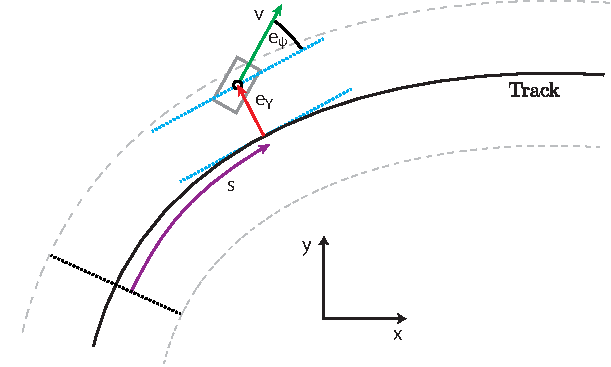
\includegraphics{../../Figures/Models/s_ey.pdf}
	\caption{Dynamic bicycle model}
	\label{fig:s_ey}
\end{figure}
The new state dynamics use the curvature $c(s)$ to describe the shape of the race track. The curvature is defined as the inverse of the curve radius
\begin{equation}
c(s) = \frac{1}{r(s)}.
\end{equation}
For a race track given in global coordinates $x(s)$ and $y(s)$, the curvature can be calculated by
\begin{equation}
c = \frac{x'y''-y'x''}{(x'^2+y'^2)^\frac{3}{2}}.
\end{equation}
The state dynamics of the \emph{kinematic model} in the track frame are derived as follows (refer to \cite{rajamani2005vehicle}):
\begin{subequations}\label{eq:kinTrackModel}
\begin{align}
    \dot s &= v\cdot \frac{\cos(e_\psi+\beta)}{1-e_Y\cdot c(s)}\\
    \dot e_Y &= v \cdot \sin(e_\psi+\beta)\\
    \dot e_\psi &= \frac{v}{L_F}\cdot \sin(\beta)-v\cdot c(s)\cdot \frac{\cos(e_\psi+\beta)}{1-e_Y\cdot c(s)}\\
    \dot v &= a
\end{align}
\end{subequations}
The \emph{dynamic bicycle model} in the track frame is described by following equations:
\begin{subequations}\label{eq:dynTrackModel}
\begin{align}
    \dot e_Y &= v_x\cdot \sin(e_\psi) + v_y\cdot \cos(e_\psi)\\
    \dot e_\psi &= \dot\psi - c(s)\cdot\frac{v_x\cos(e_\psi)-v_y\sin(e_\psi)}{1-e_Y\cdot c(s)}
\end{align}
\end{subequations}
We are going to use the models of Eq. \eqref{eq:kinTrackModel} and Eq. \eqref{eq:dynTrackModel} for all further simulations in combination with a given racetrack, i.e. a given curvature function $c(s)$.
\section{LMPC formulation}
This section presents the LMPC formulation of the race driving problem. In general, race driving is a minimum time problem: The variable that is to be optimized is the time the car takes to drive from the start to the finish line.\\
We use the dynamic bicycle model with following states and inputs:
\begin{align}
\bm{x}_t^j&=\begin{pmatrix}
v_{x,t}^j & v_{y,t}^j & \dot \psi_t^j & e_{\psi,t}^j & e_{y,t}^j & s_t^j
\end{pmatrix}^T\\
\bm{u}_t^j&=\begin{pmatrix}
a_t^j & \delta_t^j
\end{pmatrix}^T,
\end{align}
and Eq. \eqref{eq:generalLMPC} as the optimization function.
% Are there other ways on how to formulate this problem?
The racing problem is formulated by using a constant cost function whenever the car is located between the start and finish line and zero cost when the car has crossed the finish line \cite{Rosolia2016}. Thus the stage cost is defined as follows:
\begin{equation}
h(\bm{x}_t,\bm{u}_t)=\begin{cases}
1&\text{if }\bm{x}_t\not\in\mathcal{X}_F,\\
0&\text{if }\bm{x}_t\in\mathcal{X}_F,
\end{cases}
\end{equation}
where $\mathcal{X}_F$ is the set of points beyond the finish line at $s_{target}$:
\begin{equation}
\mathcal{X}_F=\left\{\bm{x}\in \mathbb{R}^6: \bm{xe}_6^T=s>s_{target}\right\},
\end{equation}
where $e_6$ is the 6-th standard basis in $\mathbb{R}^6$.\\
Lane boundaries are modeled as state constraints on the lateral position error $e_Y$:
\begin{equation}
-\frac{w_{Lane}}{2}\leq e_Y \leq \frac{w_{Lane}}{2},
\end{equation}
with lane width $w_{Lane}$.

\section{Approximation of the safe set and LP relaxation}
% Note: This has to be adapted according to the 'new' LMPC strategy, stacking two iterations together.
The LMPC problem from \eqref{eq:generalLMPC} minimizes its objective function over the safe set $\mathcal{SS}$. Since the safe set is a set of discrete states of previous iterations, this formulation is a Mixed Integer Nonlinear Programming (MINLP) problem. As this type of problem is generally computationally challenging, we introduce the concept of safe set relaxation to transform the MINLP to a continuous problem.\\
For this purpose, we approximate the safe set and its cost function using a convex combination of two polynomials as in \cite{RosoliaRacing}.

We define the time varying approximated safe set $\tilde{\mathcal{SS}}_t^{j,j-1}$ as follows:
\begin{equation}
\tilde{\mathcal{SS}}_t^{j,j-1} = \left\{\bm{x}\in\mathbb{R}^5,\lambda\in[0,1]: \bm{x}\in\lambda \tilde{\bm{x}}_t^{j,j-1}+(1-\lambda)\tilde{\bm{x}}_t^{j,j-2}\right\}
\end{equation}
where $\tilde{\bm{x}}_t^{j,k}$ is an $n$-th degree polynomial that approximates the $k$-th trajectory locally:
\begin{equation}
\tilde{\bm{x}}_t^{j,k}=\left\{\bm{x}\in\mathbb{R}^5:\forall i\in\{v_x,v_y,\dot\psi,e_\psi,e_y\},i=\begin{pmatrix}s^n &s^{n-1}&...&s& 1\end{pmatrix}\bm{\Gamma}_{t,i}^{j,k}\right\},
\end{equation}
where $\bm{\Gamma}_{t,i}^{j,k}$ is a vector containing the coefficients of the polynomial at time $t$.\\
We also define the time varying function $C_t^{j,k}(\cdot)$ to approximate the cost-to-go function $J_{t\rightarrow\infty}^k(\cdot)$:
\begin{equation}
C_t^{j,k}(\bm{x})=\begin{cases}
\begin{pmatrix}
s^n & s^{n-1} &...&s&1
\end{pmatrix}
\bm{\Delta}_t^{j,k},&\text{if } \bm{x}\in\tilde{\bm{x}}_t^{j,k},\\
+\infty,&\text{if } \bm{x}\not\in\tilde{\bm{x}}_t^{j,k},
\end{cases}
\end{equation}
where $\bm{\Delta}_t^{j,k}$ contains the coefficients of the polynomial approximating the cost-to-go in iteration $k$.\\
We define the continuous time varying approximation of $Q^{j-1}(\cdot)$:
\begin{equation}
\tilde Q_t^{j,j-1}(\bm{x},\lambda)=\begin{cases}
\lambda C_t^{j,j-1}(\bm{x})+(1-\lambda)C_t^{j,j-2}(\bm{x}),&\text{if }(\bm{x},\lambda)\in\tilde{\mathcal{SS}}_t^{j,j-1},\\
+\infty,&\text{if }(\bm{x},\lambda)\not\in\tilde{\mathcal{SS}}_t^{j,j-1}.
\end{cases}
\end{equation}
Having defined the relaxation of the safe set and approximation of the terminal cost function we can rewrite the LMPC formulation from Eq. \eqref{eq:generalLMPC}:
\begin{subequations}
\begin{align}
\tilde{J}_{t\rightarrow t+N}^{\scalebox{0.4}{LMPC},j}(\bm{x}_t^j)&=\min_{\lambda,\bm{u}_{t|t},...,\bm{u}_{t+N-1|t}}\left[\sum_{k=t}^{t+N-1}h(\bm{x}_{k|t},u_{k|t})+\tilde{Q}^{j,j-1}(\bm{x}_{t+N|t},\lambda)\right]\\
\text{s.t.}\notag\\
\bm{x}_{k+1|t}&=f(\bm{x}_{k|t},\bm{u}_{k|t}),\forall k\in[t,...,t+N],\\
\bm{x}_{t|t}&=\bm{x}_t^j,\\
\bm{x}_{k|t}&\in\mathcal{X},\bm{u}_k\in\mathcal{U},\forall k\in[t,...,t+N],\\
(\bm{x}_{t+N|t},\lambda)&\in\tilde{\mathcal{SS}}^{j,j-1}.
\end{align}\label{eq:relaxedLMPC}
\end{subequations}
In practice, the polynomial degree $n$ as well as the number of points that are used for the approximation are design parameters. The polynomial degree has to be chosen large enough to approximate the trajectory in the chosen area well enough. However, a high degree polynomial function can lead to numerical difficulties for the solver due to large derivative values and multiple local minima. Similarly, the number of points has to be chosen in such a way that the predicted terminal state $\bm{x}_N$ lies inside the approximated area. This is why this method works especially well if the approximated region is not too large (i.e. if the horizon $N$ is not too long) and if the trajectories can be well approximated by polynomials of the chosen degree.\\
For simulations and experiments in this thesis, a polynomial degree of $n=4...6$ proved to work well.\\
In the case of no model mismatch it would be sufficient to use only the previous iteration in the safe set.
However, since we expect some model mismatch in experiments, we always select the previous iteration as well as a second iteration with lowest iteration cost for the relaxation of the safe set and the approximation and the Q function.\\
In general, this approach could be extended to using more than two trajectories in the safe set. However, this would require more than one coefficient $\lambda$ and make the optimization problem more complex.
%\begin{itemize}
%\item Notes about how to choose the correct degree and horizon for polynomial approximation
%\item LMPC is a MIP (have to minimize over Q functions of discrete trajectories and their terminal constraints)
%\item Idea: approximate safe set trajectories with polynomials and minimize over convex combination of these polynomials
%\item In general: Since principle of non decreasing cost, only the last trajectory would be enough
%\item In practice: Assuming model mismatch, so use multiple previous trajectories
%\item To make computation efficient: Only use two iterations (last one and the other best previous one).
%\item Question: Is it proved that we get decreasing iteration cost for model mismatch? Why do we have to use the last one? Because otherwise we would get stuck with the best two? Mathematical explanation? - No, it's not proved yet. But people are working on it (Robust LMPC), 01/18/2017.
%\item Discussion of the relaxation method: It works well for low order polynomials, short horizons and smooth safe set trajectories. If the horizon is too long, the polynomial might not be able to approximate the safe set well enough. However, if we choose a higher degree polynomial that is able to approximate the safe set better, the solver will have a hard time since there are large first derivatives and many local optima.
%\item Discussion on how to theoretically use all previous trajectories in the safe set: Will have to introduce more $\lambda$.
%\item Also for Introduction: Important point about model mismatch: One huge advantage of using LMPC and system ID is that we can learn even the model during repeating iterations since we're getting a better and better model by the Linear Regression and the safe set is getting better and better as well.
%\end{itemize}

\section{Simulations}
The LMPC strategy is applied on the kinematic and the dynamic model in the track frame. The results are then mapped to the inertial $x-y$ frame to visualize the trajectory.\\
The physical parameters of the model are taken from a 1:10 scale RC car that is also used for real experiments. They are listed in Tab. \ref{tab:BARCPar}.

\begin{table}
\centering
\caption{Simulation parameters}\label{tab:BARCPar}
\begin{tabular}{l|l}
Parameter & Value\\
\hline
Mass& $m=\SI{2.0}{\kilo\gram}$\\
Axle distances&$L_F=L_R = \SI{0.125}{\meter}$\\
Moment of inertia&$I_z = \SI{0.03}{\kilo\gram\square\meter}$
\end{tabular}
\end{table}
%\emph{Note:} In the MPC formulation the Pacejka function is approximated by a linear function that is constrained to maximum tire forces. This linearization simplifies the optimization problem while still modeling the tire forces depending on the tire slip angles. % not valid anymore
The curvature $c(s)$ is given and constructed in such a way that the track is closed (finish line = start line). It is modeled as a piecewise linear and continuous function. At each time step, the curvature is locally approximated by a polynomial. This approximation is needed in the control formulation to allow a smooth prediction of the curvature at every $s$. The curvature used for simulations is shown in Fig. \ref{fig:Sim_curv}. Negative curvatures are interpreted as right turns, positive curvatures as left turns. The track used for simulations has a length of $s_{Total} = \SI{50.49}{\meter}$.\\
\emph{Note:} Constructing the curvature $c(s)$ by a piecewise polynomial function (polynomial degree $n>1$) and thus making it differentiable could improve the approximation by polynomials even more. However, using a piecewise linear function proved to yield good results for our application.
\begin{figure}[ht]
	\centering
  	%% Creator: Matplotlib, PGF backend
%%
%% To include the figure in your LaTeX document, write
%%   \input{<filename>.pgf}
%%
%% Make sure the required packages are loaded in your preamble
%%   \usepackage{pgf}
%%
%% Figures using additional raster images can only be included by \input if
%% they are in the same directory as the main LaTeX file. For loading figures
%% from other directories you can use the `import` package
%%   \usepackage{import}
%% and then include the figures with
%%   \import{<path to file>}{<filename>.pgf}
%%
%% Matplotlib used the following preamble
%%   \usepackage{fontspec}
%%
\begingroup%
\makeatletter%
\begin{pgfpicture}%
\pgfpathrectangle{\pgfpointorigin}{\pgfqpoint{5.500000in}{3.000000in}}%
\pgfusepath{use as bounding box, clip}%
\begin{pgfscope}%
\pgfsetbuttcap%
\pgfsetmiterjoin%
\definecolor{currentfill}{rgb}{1.000000,1.000000,1.000000}%
\pgfsetfillcolor{currentfill}%
\pgfsetlinewidth{0.000000pt}%
\definecolor{currentstroke}{rgb}{1.000000,1.000000,1.000000}%
\pgfsetstrokecolor{currentstroke}%
\pgfsetdash{}{0pt}%
\pgfpathmoveto{\pgfqpoint{0.000000in}{0.000000in}}%
\pgfpathlineto{\pgfqpoint{5.500000in}{0.000000in}}%
\pgfpathlineto{\pgfqpoint{5.500000in}{3.000000in}}%
\pgfpathlineto{\pgfqpoint{0.000000in}{3.000000in}}%
\pgfpathclose%
\pgfusepath{fill}%
\end{pgfscope}%
\begin{pgfscope}%
\pgfsetbuttcap%
\pgfsetmiterjoin%
\definecolor{currentfill}{rgb}{1.000000,1.000000,1.000000}%
\pgfsetfillcolor{currentfill}%
\pgfsetlinewidth{0.000000pt}%
\definecolor{currentstroke}{rgb}{0.000000,0.000000,0.000000}%
\pgfsetstrokecolor{currentstroke}%
\pgfsetstrokeopacity{0.000000}%
\pgfsetdash{}{0pt}%
\pgfpathmoveto{\pgfqpoint{0.665614in}{0.471921in}}%
\pgfpathlineto{\pgfqpoint{5.291316in}{0.471921in}}%
\pgfpathlineto{\pgfqpoint{5.291316in}{2.805251in}}%
\pgfpathlineto{\pgfqpoint{0.665614in}{2.805251in}}%
\pgfpathclose%
\pgfusepath{fill}%
\end{pgfscope}%
\begin{pgfscope}%
\pgfpathrectangle{\pgfqpoint{0.665614in}{0.471921in}}{\pgfqpoint{4.625702in}{2.333330in}} %
\pgfusepath{clip}%
\pgfsetrectcap%
\pgfsetroundjoin%
\pgfsetlinewidth{0.501875pt}%
\definecolor{currentstroke}{rgb}{0.000000,0.000000,1.000000}%
\pgfsetstrokecolor{currentstroke}%
\pgfsetdash{}{0pt}%
\pgfpathmoveto{\pgfqpoint{0.666385in}{1.871919in}}%
\pgfpathlineto{\pgfqpoint{0.820575in}{1.871919in}}%
\pgfpathlineto{\pgfqpoint{0.974765in}{1.138882in}}%
\pgfpathlineto{\pgfqpoint{1.128955in}{1.871919in}}%
\pgfpathlineto{\pgfqpoint{1.206050in}{1.871919in}}%
\pgfpathlineto{\pgfqpoint{1.360240in}{1.138882in}}%
\pgfpathlineto{\pgfqpoint{1.514430in}{1.871919in}}%
\pgfpathlineto{\pgfqpoint{1.591525in}{1.138882in}}%
\pgfpathlineto{\pgfqpoint{1.668621in}{1.871919in}}%
\pgfpathlineto{\pgfqpoint{1.899906in}{1.871919in}}%
\pgfpathlineto{\pgfqpoint{2.285381in}{2.604956in}}%
\pgfpathlineto{\pgfqpoint{2.672398in}{1.865381in}}%
\pgfpathlineto{\pgfqpoint{2.902141in}{0.894536in}}%
\pgfpathlineto{\pgfqpoint{3.133426in}{1.871919in}}%
\pgfpathlineto{\pgfqpoint{3.364711in}{1.871919in}}%
\pgfpathlineto{\pgfqpoint{3.518901in}{1.138882in}}%
\pgfpathlineto{\pgfqpoint{3.673092in}{1.871919in}}%
\pgfpathlineto{\pgfqpoint{3.781025in}{1.871919in}}%
\pgfpathlineto{\pgfqpoint{4.012310in}{1.383228in}}%
\pgfpathlineto{\pgfqpoint{4.243595in}{1.871919in}}%
\pgfpathlineto{\pgfqpoint{4.587439in}{1.871919in}}%
\pgfpathlineto{\pgfqpoint{4.587439in}{1.871919in}}%
\pgfusepath{stroke}%
\end{pgfscope}%
\begin{pgfscope}%
\pgfsetrectcap%
\pgfsetmiterjoin%
\pgfsetlinewidth{0.501875pt}%
\definecolor{currentstroke}{rgb}{0.000000,0.000000,0.000000}%
\pgfsetstrokecolor{currentstroke}%
\pgfsetdash{}{0pt}%
\pgfpathmoveto{\pgfqpoint{0.665614in}{2.805251in}}%
\pgfpathlineto{\pgfqpoint{5.291316in}{2.805251in}}%
\pgfusepath{stroke}%
\end{pgfscope}%
\begin{pgfscope}%
\pgfsetrectcap%
\pgfsetmiterjoin%
\pgfsetlinewidth{0.501875pt}%
\definecolor{currentstroke}{rgb}{0.000000,0.000000,0.000000}%
\pgfsetstrokecolor{currentstroke}%
\pgfsetdash{}{0pt}%
\pgfpathmoveto{\pgfqpoint{5.291316in}{0.471921in}}%
\pgfpathlineto{\pgfqpoint{5.291316in}{2.805251in}}%
\pgfusepath{stroke}%
\end{pgfscope}%
\begin{pgfscope}%
\pgfsetrectcap%
\pgfsetmiterjoin%
\pgfsetlinewidth{0.501875pt}%
\definecolor{currentstroke}{rgb}{0.000000,0.000000,0.000000}%
\pgfsetstrokecolor{currentstroke}%
\pgfsetdash{}{0pt}%
\pgfpathmoveto{\pgfqpoint{0.665614in}{0.471921in}}%
\pgfpathlineto{\pgfqpoint{5.291316in}{0.471921in}}%
\pgfusepath{stroke}%
\end{pgfscope}%
\begin{pgfscope}%
\pgfsetrectcap%
\pgfsetmiterjoin%
\pgfsetlinewidth{0.501875pt}%
\definecolor{currentstroke}{rgb}{0.000000,0.000000,0.000000}%
\pgfsetstrokecolor{currentstroke}%
\pgfsetdash{}{0pt}%
\pgfpathmoveto{\pgfqpoint{0.665614in}{0.471921in}}%
\pgfpathlineto{\pgfqpoint{0.665614in}{2.805251in}}%
\pgfusepath{stroke}%
\end{pgfscope}%
\begin{pgfscope}%
\pgfpathrectangle{\pgfqpoint{0.665614in}{0.471921in}}{\pgfqpoint{4.625702in}{2.333330in}} %
\pgfusepath{clip}%
\pgfsetbuttcap%
\pgfsetroundjoin%
\pgfsetlinewidth{0.501875pt}%
\definecolor{currentstroke}{rgb}{0.000000,0.000000,0.000000}%
\pgfsetstrokecolor{currentstroke}%
\pgfsetdash{{1.000000pt}{3.000000pt}}{0.000000pt}%
\pgfpathmoveto{\pgfqpoint{0.665614in}{0.471921in}}%
\pgfpathlineto{\pgfqpoint{0.665614in}{2.805251in}}%
\pgfusepath{stroke}%
\end{pgfscope}%
\begin{pgfscope}%
\pgfsetbuttcap%
\pgfsetroundjoin%
\definecolor{currentfill}{rgb}{0.000000,0.000000,0.000000}%
\pgfsetfillcolor{currentfill}%
\pgfsetlinewidth{0.250937pt}%
\definecolor{currentstroke}{rgb}{0.000000,0.000000,0.000000}%
\pgfsetstrokecolor{currentstroke}%
\pgfsetdash{}{0pt}%
\pgfsys@defobject{currentmarker}{\pgfqpoint{0.000000in}{0.000000in}}{\pgfqpoint{0.000000in}{0.055556in}}{%
\pgfpathmoveto{\pgfqpoint{0.000000in}{0.000000in}}%
\pgfpathlineto{\pgfqpoint{0.000000in}{0.055556in}}%
\pgfusepath{stroke,fill}%
}%
\begin{pgfscope}%
\pgfsys@transformshift{0.665614in}{0.471921in}%
\pgfsys@useobject{currentmarker}{}%
\end{pgfscope}%
\end{pgfscope}%
\begin{pgfscope}%
\pgfsetbuttcap%
\pgfsetroundjoin%
\definecolor{currentfill}{rgb}{0.000000,0.000000,0.000000}%
\pgfsetfillcolor{currentfill}%
\pgfsetlinewidth{0.250937pt}%
\definecolor{currentstroke}{rgb}{0.000000,0.000000,0.000000}%
\pgfsetstrokecolor{currentstroke}%
\pgfsetdash{}{0pt}%
\pgfsys@defobject{currentmarker}{\pgfqpoint{0.000000in}{-0.055556in}}{\pgfqpoint{0.000000in}{0.000000in}}{%
\pgfpathmoveto{\pgfqpoint{0.000000in}{0.000000in}}%
\pgfpathlineto{\pgfqpoint{0.000000in}{-0.055556in}}%
\pgfusepath{stroke,fill}%
}%
\begin{pgfscope}%
\pgfsys@transformshift{0.665614in}{2.805251in}%
\pgfsys@useobject{currentmarker}{}%
\end{pgfscope}%
\end{pgfscope}%
\begin{pgfscope}%
\pgftext[x=0.665614in,y=0.416365in,,top]{\rmfamily\fontsize{6.940000}{8.328000}\selectfont \(\displaystyle 0\)}%
\end{pgfscope}%
\begin{pgfscope}%
\pgfpathrectangle{\pgfqpoint{0.665614in}{0.471921in}}{\pgfqpoint{4.625702in}{2.333330in}} %
\pgfusepath{clip}%
\pgfsetbuttcap%
\pgfsetroundjoin%
\pgfsetlinewidth{0.501875pt}%
\definecolor{currentstroke}{rgb}{0.000000,0.000000,0.000000}%
\pgfsetstrokecolor{currentstroke}%
\pgfsetdash{{1.000000pt}{3.000000pt}}{0.000000pt}%
\pgfpathmoveto{\pgfqpoint{1.436564in}{0.471921in}}%
\pgfpathlineto{\pgfqpoint{1.436564in}{2.805251in}}%
\pgfusepath{stroke}%
\end{pgfscope}%
\begin{pgfscope}%
\pgfsetbuttcap%
\pgfsetroundjoin%
\definecolor{currentfill}{rgb}{0.000000,0.000000,0.000000}%
\pgfsetfillcolor{currentfill}%
\pgfsetlinewidth{0.250937pt}%
\definecolor{currentstroke}{rgb}{0.000000,0.000000,0.000000}%
\pgfsetstrokecolor{currentstroke}%
\pgfsetdash{}{0pt}%
\pgfsys@defobject{currentmarker}{\pgfqpoint{0.000000in}{0.000000in}}{\pgfqpoint{0.000000in}{0.055556in}}{%
\pgfpathmoveto{\pgfqpoint{0.000000in}{0.000000in}}%
\pgfpathlineto{\pgfqpoint{0.000000in}{0.055556in}}%
\pgfusepath{stroke,fill}%
}%
\begin{pgfscope}%
\pgfsys@transformshift{1.436564in}{0.471921in}%
\pgfsys@useobject{currentmarker}{}%
\end{pgfscope}%
\end{pgfscope}%
\begin{pgfscope}%
\pgfsetbuttcap%
\pgfsetroundjoin%
\definecolor{currentfill}{rgb}{0.000000,0.000000,0.000000}%
\pgfsetfillcolor{currentfill}%
\pgfsetlinewidth{0.250937pt}%
\definecolor{currentstroke}{rgb}{0.000000,0.000000,0.000000}%
\pgfsetstrokecolor{currentstroke}%
\pgfsetdash{}{0pt}%
\pgfsys@defobject{currentmarker}{\pgfqpoint{0.000000in}{-0.055556in}}{\pgfqpoint{0.000000in}{0.000000in}}{%
\pgfpathmoveto{\pgfqpoint{0.000000in}{0.000000in}}%
\pgfpathlineto{\pgfqpoint{0.000000in}{-0.055556in}}%
\pgfusepath{stroke,fill}%
}%
\begin{pgfscope}%
\pgfsys@transformshift{1.436564in}{2.805251in}%
\pgfsys@useobject{currentmarker}{}%
\end{pgfscope}%
\end{pgfscope}%
\begin{pgfscope}%
\pgftext[x=1.436564in,y=0.416365in,,top]{\rmfamily\fontsize{6.940000}{8.328000}\selectfont \(\displaystyle 10\)}%
\end{pgfscope}%
\begin{pgfscope}%
\pgfpathrectangle{\pgfqpoint{0.665614in}{0.471921in}}{\pgfqpoint{4.625702in}{2.333330in}} %
\pgfusepath{clip}%
\pgfsetbuttcap%
\pgfsetroundjoin%
\pgfsetlinewidth{0.501875pt}%
\definecolor{currentstroke}{rgb}{0.000000,0.000000,0.000000}%
\pgfsetstrokecolor{currentstroke}%
\pgfsetdash{{1.000000pt}{3.000000pt}}{0.000000pt}%
\pgfpathmoveto{\pgfqpoint{2.207515in}{0.471921in}}%
\pgfpathlineto{\pgfqpoint{2.207515in}{2.805251in}}%
\pgfusepath{stroke}%
\end{pgfscope}%
\begin{pgfscope}%
\pgfsetbuttcap%
\pgfsetroundjoin%
\definecolor{currentfill}{rgb}{0.000000,0.000000,0.000000}%
\pgfsetfillcolor{currentfill}%
\pgfsetlinewidth{0.250937pt}%
\definecolor{currentstroke}{rgb}{0.000000,0.000000,0.000000}%
\pgfsetstrokecolor{currentstroke}%
\pgfsetdash{}{0pt}%
\pgfsys@defobject{currentmarker}{\pgfqpoint{0.000000in}{0.000000in}}{\pgfqpoint{0.000000in}{0.055556in}}{%
\pgfpathmoveto{\pgfqpoint{0.000000in}{0.000000in}}%
\pgfpathlineto{\pgfqpoint{0.000000in}{0.055556in}}%
\pgfusepath{stroke,fill}%
}%
\begin{pgfscope}%
\pgfsys@transformshift{2.207515in}{0.471921in}%
\pgfsys@useobject{currentmarker}{}%
\end{pgfscope}%
\end{pgfscope}%
\begin{pgfscope}%
\pgfsetbuttcap%
\pgfsetroundjoin%
\definecolor{currentfill}{rgb}{0.000000,0.000000,0.000000}%
\pgfsetfillcolor{currentfill}%
\pgfsetlinewidth{0.250937pt}%
\definecolor{currentstroke}{rgb}{0.000000,0.000000,0.000000}%
\pgfsetstrokecolor{currentstroke}%
\pgfsetdash{}{0pt}%
\pgfsys@defobject{currentmarker}{\pgfqpoint{0.000000in}{-0.055556in}}{\pgfqpoint{0.000000in}{0.000000in}}{%
\pgfpathmoveto{\pgfqpoint{0.000000in}{0.000000in}}%
\pgfpathlineto{\pgfqpoint{0.000000in}{-0.055556in}}%
\pgfusepath{stroke,fill}%
}%
\begin{pgfscope}%
\pgfsys@transformshift{2.207515in}{2.805251in}%
\pgfsys@useobject{currentmarker}{}%
\end{pgfscope}%
\end{pgfscope}%
\begin{pgfscope}%
\pgftext[x=2.207515in,y=0.416365in,,top]{\rmfamily\fontsize{6.940000}{8.328000}\selectfont \(\displaystyle 20\)}%
\end{pgfscope}%
\begin{pgfscope}%
\pgfpathrectangle{\pgfqpoint{0.665614in}{0.471921in}}{\pgfqpoint{4.625702in}{2.333330in}} %
\pgfusepath{clip}%
\pgfsetbuttcap%
\pgfsetroundjoin%
\pgfsetlinewidth{0.501875pt}%
\definecolor{currentstroke}{rgb}{0.000000,0.000000,0.000000}%
\pgfsetstrokecolor{currentstroke}%
\pgfsetdash{{1.000000pt}{3.000000pt}}{0.000000pt}%
\pgfpathmoveto{\pgfqpoint{2.978465in}{0.471921in}}%
\pgfpathlineto{\pgfqpoint{2.978465in}{2.805251in}}%
\pgfusepath{stroke}%
\end{pgfscope}%
\begin{pgfscope}%
\pgfsetbuttcap%
\pgfsetroundjoin%
\definecolor{currentfill}{rgb}{0.000000,0.000000,0.000000}%
\pgfsetfillcolor{currentfill}%
\pgfsetlinewidth{0.250937pt}%
\definecolor{currentstroke}{rgb}{0.000000,0.000000,0.000000}%
\pgfsetstrokecolor{currentstroke}%
\pgfsetdash{}{0pt}%
\pgfsys@defobject{currentmarker}{\pgfqpoint{0.000000in}{0.000000in}}{\pgfqpoint{0.000000in}{0.055556in}}{%
\pgfpathmoveto{\pgfqpoint{0.000000in}{0.000000in}}%
\pgfpathlineto{\pgfqpoint{0.000000in}{0.055556in}}%
\pgfusepath{stroke,fill}%
}%
\begin{pgfscope}%
\pgfsys@transformshift{2.978465in}{0.471921in}%
\pgfsys@useobject{currentmarker}{}%
\end{pgfscope}%
\end{pgfscope}%
\begin{pgfscope}%
\pgfsetbuttcap%
\pgfsetroundjoin%
\definecolor{currentfill}{rgb}{0.000000,0.000000,0.000000}%
\pgfsetfillcolor{currentfill}%
\pgfsetlinewidth{0.250937pt}%
\definecolor{currentstroke}{rgb}{0.000000,0.000000,0.000000}%
\pgfsetstrokecolor{currentstroke}%
\pgfsetdash{}{0pt}%
\pgfsys@defobject{currentmarker}{\pgfqpoint{0.000000in}{-0.055556in}}{\pgfqpoint{0.000000in}{0.000000in}}{%
\pgfpathmoveto{\pgfqpoint{0.000000in}{0.000000in}}%
\pgfpathlineto{\pgfqpoint{0.000000in}{-0.055556in}}%
\pgfusepath{stroke,fill}%
}%
\begin{pgfscope}%
\pgfsys@transformshift{2.978465in}{2.805251in}%
\pgfsys@useobject{currentmarker}{}%
\end{pgfscope}%
\end{pgfscope}%
\begin{pgfscope}%
\pgftext[x=2.978465in,y=0.416365in,,top]{\rmfamily\fontsize{6.940000}{8.328000}\selectfont \(\displaystyle 30\)}%
\end{pgfscope}%
\begin{pgfscope}%
\pgfpathrectangle{\pgfqpoint{0.665614in}{0.471921in}}{\pgfqpoint{4.625702in}{2.333330in}} %
\pgfusepath{clip}%
\pgfsetbuttcap%
\pgfsetroundjoin%
\pgfsetlinewidth{0.501875pt}%
\definecolor{currentstroke}{rgb}{0.000000,0.000000,0.000000}%
\pgfsetstrokecolor{currentstroke}%
\pgfsetdash{{1.000000pt}{3.000000pt}}{0.000000pt}%
\pgfpathmoveto{\pgfqpoint{3.749416in}{0.471921in}}%
\pgfpathlineto{\pgfqpoint{3.749416in}{2.805251in}}%
\pgfusepath{stroke}%
\end{pgfscope}%
\begin{pgfscope}%
\pgfsetbuttcap%
\pgfsetroundjoin%
\definecolor{currentfill}{rgb}{0.000000,0.000000,0.000000}%
\pgfsetfillcolor{currentfill}%
\pgfsetlinewidth{0.250937pt}%
\definecolor{currentstroke}{rgb}{0.000000,0.000000,0.000000}%
\pgfsetstrokecolor{currentstroke}%
\pgfsetdash{}{0pt}%
\pgfsys@defobject{currentmarker}{\pgfqpoint{0.000000in}{0.000000in}}{\pgfqpoint{0.000000in}{0.055556in}}{%
\pgfpathmoveto{\pgfqpoint{0.000000in}{0.000000in}}%
\pgfpathlineto{\pgfqpoint{0.000000in}{0.055556in}}%
\pgfusepath{stroke,fill}%
}%
\begin{pgfscope}%
\pgfsys@transformshift{3.749416in}{0.471921in}%
\pgfsys@useobject{currentmarker}{}%
\end{pgfscope}%
\end{pgfscope}%
\begin{pgfscope}%
\pgfsetbuttcap%
\pgfsetroundjoin%
\definecolor{currentfill}{rgb}{0.000000,0.000000,0.000000}%
\pgfsetfillcolor{currentfill}%
\pgfsetlinewidth{0.250937pt}%
\definecolor{currentstroke}{rgb}{0.000000,0.000000,0.000000}%
\pgfsetstrokecolor{currentstroke}%
\pgfsetdash{}{0pt}%
\pgfsys@defobject{currentmarker}{\pgfqpoint{0.000000in}{-0.055556in}}{\pgfqpoint{0.000000in}{0.000000in}}{%
\pgfpathmoveto{\pgfqpoint{0.000000in}{0.000000in}}%
\pgfpathlineto{\pgfqpoint{0.000000in}{-0.055556in}}%
\pgfusepath{stroke,fill}%
}%
\begin{pgfscope}%
\pgfsys@transformshift{3.749416in}{2.805251in}%
\pgfsys@useobject{currentmarker}{}%
\end{pgfscope}%
\end{pgfscope}%
\begin{pgfscope}%
\pgftext[x=3.749416in,y=0.416365in,,top]{\rmfamily\fontsize{6.940000}{8.328000}\selectfont \(\displaystyle 40\)}%
\end{pgfscope}%
\begin{pgfscope}%
\pgfpathrectangle{\pgfqpoint{0.665614in}{0.471921in}}{\pgfqpoint{4.625702in}{2.333330in}} %
\pgfusepath{clip}%
\pgfsetbuttcap%
\pgfsetroundjoin%
\pgfsetlinewidth{0.501875pt}%
\definecolor{currentstroke}{rgb}{0.000000,0.000000,0.000000}%
\pgfsetstrokecolor{currentstroke}%
\pgfsetdash{{1.000000pt}{3.000000pt}}{0.000000pt}%
\pgfpathmoveto{\pgfqpoint{4.520366in}{0.471921in}}%
\pgfpathlineto{\pgfqpoint{4.520366in}{2.805251in}}%
\pgfusepath{stroke}%
\end{pgfscope}%
\begin{pgfscope}%
\pgfsetbuttcap%
\pgfsetroundjoin%
\definecolor{currentfill}{rgb}{0.000000,0.000000,0.000000}%
\pgfsetfillcolor{currentfill}%
\pgfsetlinewidth{0.250937pt}%
\definecolor{currentstroke}{rgb}{0.000000,0.000000,0.000000}%
\pgfsetstrokecolor{currentstroke}%
\pgfsetdash{}{0pt}%
\pgfsys@defobject{currentmarker}{\pgfqpoint{0.000000in}{0.000000in}}{\pgfqpoint{0.000000in}{0.055556in}}{%
\pgfpathmoveto{\pgfqpoint{0.000000in}{0.000000in}}%
\pgfpathlineto{\pgfqpoint{0.000000in}{0.055556in}}%
\pgfusepath{stroke,fill}%
}%
\begin{pgfscope}%
\pgfsys@transformshift{4.520366in}{0.471921in}%
\pgfsys@useobject{currentmarker}{}%
\end{pgfscope}%
\end{pgfscope}%
\begin{pgfscope}%
\pgfsetbuttcap%
\pgfsetroundjoin%
\definecolor{currentfill}{rgb}{0.000000,0.000000,0.000000}%
\pgfsetfillcolor{currentfill}%
\pgfsetlinewidth{0.250937pt}%
\definecolor{currentstroke}{rgb}{0.000000,0.000000,0.000000}%
\pgfsetstrokecolor{currentstroke}%
\pgfsetdash{}{0pt}%
\pgfsys@defobject{currentmarker}{\pgfqpoint{0.000000in}{-0.055556in}}{\pgfqpoint{0.000000in}{0.000000in}}{%
\pgfpathmoveto{\pgfqpoint{0.000000in}{0.000000in}}%
\pgfpathlineto{\pgfqpoint{0.000000in}{-0.055556in}}%
\pgfusepath{stroke,fill}%
}%
\begin{pgfscope}%
\pgfsys@transformshift{4.520366in}{2.805251in}%
\pgfsys@useobject{currentmarker}{}%
\end{pgfscope}%
\end{pgfscope}%
\begin{pgfscope}%
\pgftext[x=4.520366in,y=0.416365in,,top]{\rmfamily\fontsize{6.940000}{8.328000}\selectfont \(\displaystyle 50\)}%
\end{pgfscope}%
\begin{pgfscope}%
\pgfpathrectangle{\pgfqpoint{0.665614in}{0.471921in}}{\pgfqpoint{4.625702in}{2.333330in}} %
\pgfusepath{clip}%
\pgfsetbuttcap%
\pgfsetroundjoin%
\pgfsetlinewidth{0.501875pt}%
\definecolor{currentstroke}{rgb}{0.000000,0.000000,0.000000}%
\pgfsetstrokecolor{currentstroke}%
\pgfsetdash{{1.000000pt}{3.000000pt}}{0.000000pt}%
\pgfpathmoveto{\pgfqpoint{5.291316in}{0.471921in}}%
\pgfpathlineto{\pgfqpoint{5.291316in}{2.805251in}}%
\pgfusepath{stroke}%
\end{pgfscope}%
\begin{pgfscope}%
\pgfsetbuttcap%
\pgfsetroundjoin%
\definecolor{currentfill}{rgb}{0.000000,0.000000,0.000000}%
\pgfsetfillcolor{currentfill}%
\pgfsetlinewidth{0.250937pt}%
\definecolor{currentstroke}{rgb}{0.000000,0.000000,0.000000}%
\pgfsetstrokecolor{currentstroke}%
\pgfsetdash{}{0pt}%
\pgfsys@defobject{currentmarker}{\pgfqpoint{0.000000in}{0.000000in}}{\pgfqpoint{0.000000in}{0.055556in}}{%
\pgfpathmoveto{\pgfqpoint{0.000000in}{0.000000in}}%
\pgfpathlineto{\pgfqpoint{0.000000in}{0.055556in}}%
\pgfusepath{stroke,fill}%
}%
\begin{pgfscope}%
\pgfsys@transformshift{5.291316in}{0.471921in}%
\pgfsys@useobject{currentmarker}{}%
\end{pgfscope}%
\end{pgfscope}%
\begin{pgfscope}%
\pgfsetbuttcap%
\pgfsetroundjoin%
\definecolor{currentfill}{rgb}{0.000000,0.000000,0.000000}%
\pgfsetfillcolor{currentfill}%
\pgfsetlinewidth{0.250937pt}%
\definecolor{currentstroke}{rgb}{0.000000,0.000000,0.000000}%
\pgfsetstrokecolor{currentstroke}%
\pgfsetdash{}{0pt}%
\pgfsys@defobject{currentmarker}{\pgfqpoint{0.000000in}{-0.055556in}}{\pgfqpoint{0.000000in}{0.000000in}}{%
\pgfpathmoveto{\pgfqpoint{0.000000in}{0.000000in}}%
\pgfpathlineto{\pgfqpoint{0.000000in}{-0.055556in}}%
\pgfusepath{stroke,fill}%
}%
\begin{pgfscope}%
\pgfsys@transformshift{5.291316in}{2.805251in}%
\pgfsys@useobject{currentmarker}{}%
\end{pgfscope}%
\end{pgfscope}%
\begin{pgfscope}%
\pgftext[x=5.291316in,y=0.416365in,,top]{\rmfamily\fontsize{6.940000}{8.328000}\selectfont \(\displaystyle 60\)}%
\end{pgfscope}%
\begin{pgfscope}%
\pgftext[x=2.978465in,y=0.261328in,,top]{\rmfamily\fontsize{8.330000}{9.996000}\selectfont \(\displaystyle s\) [\(\displaystyle  m\)]}%
\end{pgfscope}%
\begin{pgfscope}%
\pgfpathrectangle{\pgfqpoint{0.665614in}{0.471921in}}{\pgfqpoint{4.625702in}{2.333330in}} %
\pgfusepath{clip}%
\pgfsetbuttcap%
\pgfsetroundjoin%
\pgfsetlinewidth{0.501875pt}%
\definecolor{currentstroke}{rgb}{0.000000,0.000000,0.000000}%
\pgfsetstrokecolor{currentstroke}%
\pgfsetdash{{1.000000pt}{3.000000pt}}{0.000000pt}%
\pgfpathmoveto{\pgfqpoint{0.665614in}{0.471921in}}%
\pgfpathlineto{\pgfqpoint{5.291316in}{0.471921in}}%
\pgfusepath{stroke}%
\end{pgfscope}%
\begin{pgfscope}%
\pgfsetbuttcap%
\pgfsetroundjoin%
\definecolor{currentfill}{rgb}{0.000000,0.000000,0.000000}%
\pgfsetfillcolor{currentfill}%
\pgfsetlinewidth{0.250937pt}%
\definecolor{currentstroke}{rgb}{0.000000,0.000000,0.000000}%
\pgfsetstrokecolor{currentstroke}%
\pgfsetdash{}{0pt}%
\pgfsys@defobject{currentmarker}{\pgfqpoint{0.000000in}{0.000000in}}{\pgfqpoint{0.055556in}{0.000000in}}{%
\pgfpathmoveto{\pgfqpoint{0.000000in}{0.000000in}}%
\pgfpathlineto{\pgfqpoint{0.055556in}{0.000000in}}%
\pgfusepath{stroke,fill}%
}%
\begin{pgfscope}%
\pgfsys@transformshift{0.665614in}{0.471921in}%
\pgfsys@useobject{currentmarker}{}%
\end{pgfscope}%
\end{pgfscope}%
\begin{pgfscope}%
\pgfsetbuttcap%
\pgfsetroundjoin%
\definecolor{currentfill}{rgb}{0.000000,0.000000,0.000000}%
\pgfsetfillcolor{currentfill}%
\pgfsetlinewidth{0.250937pt}%
\definecolor{currentstroke}{rgb}{0.000000,0.000000,0.000000}%
\pgfsetstrokecolor{currentstroke}%
\pgfsetdash{}{0pt}%
\pgfsys@defobject{currentmarker}{\pgfqpoint{-0.055556in}{0.000000in}}{\pgfqpoint{0.000000in}{0.000000in}}{%
\pgfpathmoveto{\pgfqpoint{0.000000in}{0.000000in}}%
\pgfpathlineto{\pgfqpoint{-0.055556in}{0.000000in}}%
\pgfusepath{stroke,fill}%
}%
\begin{pgfscope}%
\pgfsys@transformshift{5.291316in}{0.471921in}%
\pgfsys@useobject{currentmarker}{}%
\end{pgfscope}%
\end{pgfscope}%
\begin{pgfscope}%
\pgftext[x=0.610058in,y=0.471921in,right,]{\rmfamily\fontsize{6.940000}{8.328000}\selectfont \(\displaystyle -1.5\)}%
\end{pgfscope}%
\begin{pgfscope}%
\pgfpathrectangle{\pgfqpoint{0.665614in}{0.471921in}}{\pgfqpoint{4.625702in}{2.333330in}} %
\pgfusepath{clip}%
\pgfsetbuttcap%
\pgfsetroundjoin%
\pgfsetlinewidth{0.501875pt}%
\definecolor{currentstroke}{rgb}{0.000000,0.000000,0.000000}%
\pgfsetstrokecolor{currentstroke}%
\pgfsetdash{{1.000000pt}{3.000000pt}}{0.000000pt}%
\pgfpathmoveto{\pgfqpoint{0.665614in}{0.938587in}}%
\pgfpathlineto{\pgfqpoint{5.291316in}{0.938587in}}%
\pgfusepath{stroke}%
\end{pgfscope}%
\begin{pgfscope}%
\pgfsetbuttcap%
\pgfsetroundjoin%
\definecolor{currentfill}{rgb}{0.000000,0.000000,0.000000}%
\pgfsetfillcolor{currentfill}%
\pgfsetlinewidth{0.250937pt}%
\definecolor{currentstroke}{rgb}{0.000000,0.000000,0.000000}%
\pgfsetstrokecolor{currentstroke}%
\pgfsetdash{}{0pt}%
\pgfsys@defobject{currentmarker}{\pgfqpoint{0.000000in}{0.000000in}}{\pgfqpoint{0.055556in}{0.000000in}}{%
\pgfpathmoveto{\pgfqpoint{0.000000in}{0.000000in}}%
\pgfpathlineto{\pgfqpoint{0.055556in}{0.000000in}}%
\pgfusepath{stroke,fill}%
}%
\begin{pgfscope}%
\pgfsys@transformshift{0.665614in}{0.938587in}%
\pgfsys@useobject{currentmarker}{}%
\end{pgfscope}%
\end{pgfscope}%
\begin{pgfscope}%
\pgfsetbuttcap%
\pgfsetroundjoin%
\definecolor{currentfill}{rgb}{0.000000,0.000000,0.000000}%
\pgfsetfillcolor{currentfill}%
\pgfsetlinewidth{0.250937pt}%
\definecolor{currentstroke}{rgb}{0.000000,0.000000,0.000000}%
\pgfsetstrokecolor{currentstroke}%
\pgfsetdash{}{0pt}%
\pgfsys@defobject{currentmarker}{\pgfqpoint{-0.055556in}{0.000000in}}{\pgfqpoint{0.000000in}{0.000000in}}{%
\pgfpathmoveto{\pgfqpoint{0.000000in}{0.000000in}}%
\pgfpathlineto{\pgfqpoint{-0.055556in}{0.000000in}}%
\pgfusepath{stroke,fill}%
}%
\begin{pgfscope}%
\pgfsys@transformshift{5.291316in}{0.938587in}%
\pgfsys@useobject{currentmarker}{}%
\end{pgfscope}%
\end{pgfscope}%
\begin{pgfscope}%
\pgftext[x=0.610058in,y=0.938587in,right,]{\rmfamily\fontsize{6.940000}{8.328000}\selectfont \(\displaystyle -1.0\)}%
\end{pgfscope}%
\begin{pgfscope}%
\pgfpathrectangle{\pgfqpoint{0.665614in}{0.471921in}}{\pgfqpoint{4.625702in}{2.333330in}} %
\pgfusepath{clip}%
\pgfsetbuttcap%
\pgfsetroundjoin%
\pgfsetlinewidth{0.501875pt}%
\definecolor{currentstroke}{rgb}{0.000000,0.000000,0.000000}%
\pgfsetstrokecolor{currentstroke}%
\pgfsetdash{{1.000000pt}{3.000000pt}}{0.000000pt}%
\pgfpathmoveto{\pgfqpoint{0.665614in}{1.405253in}}%
\pgfpathlineto{\pgfqpoint{5.291316in}{1.405253in}}%
\pgfusepath{stroke}%
\end{pgfscope}%
\begin{pgfscope}%
\pgfsetbuttcap%
\pgfsetroundjoin%
\definecolor{currentfill}{rgb}{0.000000,0.000000,0.000000}%
\pgfsetfillcolor{currentfill}%
\pgfsetlinewidth{0.250937pt}%
\definecolor{currentstroke}{rgb}{0.000000,0.000000,0.000000}%
\pgfsetstrokecolor{currentstroke}%
\pgfsetdash{}{0pt}%
\pgfsys@defobject{currentmarker}{\pgfqpoint{0.000000in}{0.000000in}}{\pgfqpoint{0.055556in}{0.000000in}}{%
\pgfpathmoveto{\pgfqpoint{0.000000in}{0.000000in}}%
\pgfpathlineto{\pgfqpoint{0.055556in}{0.000000in}}%
\pgfusepath{stroke,fill}%
}%
\begin{pgfscope}%
\pgfsys@transformshift{0.665614in}{1.405253in}%
\pgfsys@useobject{currentmarker}{}%
\end{pgfscope}%
\end{pgfscope}%
\begin{pgfscope}%
\pgfsetbuttcap%
\pgfsetroundjoin%
\definecolor{currentfill}{rgb}{0.000000,0.000000,0.000000}%
\pgfsetfillcolor{currentfill}%
\pgfsetlinewidth{0.250937pt}%
\definecolor{currentstroke}{rgb}{0.000000,0.000000,0.000000}%
\pgfsetstrokecolor{currentstroke}%
\pgfsetdash{}{0pt}%
\pgfsys@defobject{currentmarker}{\pgfqpoint{-0.055556in}{0.000000in}}{\pgfqpoint{0.000000in}{0.000000in}}{%
\pgfpathmoveto{\pgfqpoint{0.000000in}{0.000000in}}%
\pgfpathlineto{\pgfqpoint{-0.055556in}{0.000000in}}%
\pgfusepath{stroke,fill}%
}%
\begin{pgfscope}%
\pgfsys@transformshift{5.291316in}{1.405253in}%
\pgfsys@useobject{currentmarker}{}%
\end{pgfscope}%
\end{pgfscope}%
\begin{pgfscope}%
\pgftext[x=0.610058in,y=1.405253in,right,]{\rmfamily\fontsize{6.940000}{8.328000}\selectfont \(\displaystyle -0.5\)}%
\end{pgfscope}%
\begin{pgfscope}%
\pgfpathrectangle{\pgfqpoint{0.665614in}{0.471921in}}{\pgfqpoint{4.625702in}{2.333330in}} %
\pgfusepath{clip}%
\pgfsetbuttcap%
\pgfsetroundjoin%
\pgfsetlinewidth{0.501875pt}%
\definecolor{currentstroke}{rgb}{0.000000,0.000000,0.000000}%
\pgfsetstrokecolor{currentstroke}%
\pgfsetdash{{1.000000pt}{3.000000pt}}{0.000000pt}%
\pgfpathmoveto{\pgfqpoint{0.665614in}{1.871919in}}%
\pgfpathlineto{\pgfqpoint{5.291316in}{1.871919in}}%
\pgfusepath{stroke}%
\end{pgfscope}%
\begin{pgfscope}%
\pgfsetbuttcap%
\pgfsetroundjoin%
\definecolor{currentfill}{rgb}{0.000000,0.000000,0.000000}%
\pgfsetfillcolor{currentfill}%
\pgfsetlinewidth{0.250937pt}%
\definecolor{currentstroke}{rgb}{0.000000,0.000000,0.000000}%
\pgfsetstrokecolor{currentstroke}%
\pgfsetdash{}{0pt}%
\pgfsys@defobject{currentmarker}{\pgfqpoint{0.000000in}{0.000000in}}{\pgfqpoint{0.055556in}{0.000000in}}{%
\pgfpathmoveto{\pgfqpoint{0.000000in}{0.000000in}}%
\pgfpathlineto{\pgfqpoint{0.055556in}{0.000000in}}%
\pgfusepath{stroke,fill}%
}%
\begin{pgfscope}%
\pgfsys@transformshift{0.665614in}{1.871919in}%
\pgfsys@useobject{currentmarker}{}%
\end{pgfscope}%
\end{pgfscope}%
\begin{pgfscope}%
\pgfsetbuttcap%
\pgfsetroundjoin%
\definecolor{currentfill}{rgb}{0.000000,0.000000,0.000000}%
\pgfsetfillcolor{currentfill}%
\pgfsetlinewidth{0.250937pt}%
\definecolor{currentstroke}{rgb}{0.000000,0.000000,0.000000}%
\pgfsetstrokecolor{currentstroke}%
\pgfsetdash{}{0pt}%
\pgfsys@defobject{currentmarker}{\pgfqpoint{-0.055556in}{0.000000in}}{\pgfqpoint{0.000000in}{0.000000in}}{%
\pgfpathmoveto{\pgfqpoint{0.000000in}{0.000000in}}%
\pgfpathlineto{\pgfqpoint{-0.055556in}{0.000000in}}%
\pgfusepath{stroke,fill}%
}%
\begin{pgfscope}%
\pgfsys@transformshift{5.291316in}{1.871919in}%
\pgfsys@useobject{currentmarker}{}%
\end{pgfscope}%
\end{pgfscope}%
\begin{pgfscope}%
\pgftext[x=0.610058in,y=1.871919in,right,]{\rmfamily\fontsize{6.940000}{8.328000}\selectfont \(\displaystyle 0.0\)}%
\end{pgfscope}%
\begin{pgfscope}%
\pgfpathrectangle{\pgfqpoint{0.665614in}{0.471921in}}{\pgfqpoint{4.625702in}{2.333330in}} %
\pgfusepath{clip}%
\pgfsetbuttcap%
\pgfsetroundjoin%
\pgfsetlinewidth{0.501875pt}%
\definecolor{currentstroke}{rgb}{0.000000,0.000000,0.000000}%
\pgfsetstrokecolor{currentstroke}%
\pgfsetdash{{1.000000pt}{3.000000pt}}{0.000000pt}%
\pgfpathmoveto{\pgfqpoint{0.665614in}{2.338585in}}%
\pgfpathlineto{\pgfqpoint{5.291316in}{2.338585in}}%
\pgfusepath{stroke}%
\end{pgfscope}%
\begin{pgfscope}%
\pgfsetbuttcap%
\pgfsetroundjoin%
\definecolor{currentfill}{rgb}{0.000000,0.000000,0.000000}%
\pgfsetfillcolor{currentfill}%
\pgfsetlinewidth{0.250937pt}%
\definecolor{currentstroke}{rgb}{0.000000,0.000000,0.000000}%
\pgfsetstrokecolor{currentstroke}%
\pgfsetdash{}{0pt}%
\pgfsys@defobject{currentmarker}{\pgfqpoint{0.000000in}{0.000000in}}{\pgfqpoint{0.055556in}{0.000000in}}{%
\pgfpathmoveto{\pgfqpoint{0.000000in}{0.000000in}}%
\pgfpathlineto{\pgfqpoint{0.055556in}{0.000000in}}%
\pgfusepath{stroke,fill}%
}%
\begin{pgfscope}%
\pgfsys@transformshift{0.665614in}{2.338585in}%
\pgfsys@useobject{currentmarker}{}%
\end{pgfscope}%
\end{pgfscope}%
\begin{pgfscope}%
\pgfsetbuttcap%
\pgfsetroundjoin%
\definecolor{currentfill}{rgb}{0.000000,0.000000,0.000000}%
\pgfsetfillcolor{currentfill}%
\pgfsetlinewidth{0.250937pt}%
\definecolor{currentstroke}{rgb}{0.000000,0.000000,0.000000}%
\pgfsetstrokecolor{currentstroke}%
\pgfsetdash{}{0pt}%
\pgfsys@defobject{currentmarker}{\pgfqpoint{-0.055556in}{0.000000in}}{\pgfqpoint{0.000000in}{0.000000in}}{%
\pgfpathmoveto{\pgfqpoint{0.000000in}{0.000000in}}%
\pgfpathlineto{\pgfqpoint{-0.055556in}{0.000000in}}%
\pgfusepath{stroke,fill}%
}%
\begin{pgfscope}%
\pgfsys@transformshift{5.291316in}{2.338585in}%
\pgfsys@useobject{currentmarker}{}%
\end{pgfscope}%
\end{pgfscope}%
\begin{pgfscope}%
\pgftext[x=0.610058in,y=2.338585in,right,]{\rmfamily\fontsize{6.940000}{8.328000}\selectfont \(\displaystyle 0.5\)}%
\end{pgfscope}%
\begin{pgfscope}%
\pgfpathrectangle{\pgfqpoint{0.665614in}{0.471921in}}{\pgfqpoint{4.625702in}{2.333330in}} %
\pgfusepath{clip}%
\pgfsetbuttcap%
\pgfsetroundjoin%
\pgfsetlinewidth{0.501875pt}%
\definecolor{currentstroke}{rgb}{0.000000,0.000000,0.000000}%
\pgfsetstrokecolor{currentstroke}%
\pgfsetdash{{1.000000pt}{3.000000pt}}{0.000000pt}%
\pgfpathmoveto{\pgfqpoint{0.665614in}{2.805251in}}%
\pgfpathlineto{\pgfqpoint{5.291316in}{2.805251in}}%
\pgfusepath{stroke}%
\end{pgfscope}%
\begin{pgfscope}%
\pgfsetbuttcap%
\pgfsetroundjoin%
\definecolor{currentfill}{rgb}{0.000000,0.000000,0.000000}%
\pgfsetfillcolor{currentfill}%
\pgfsetlinewidth{0.250937pt}%
\definecolor{currentstroke}{rgb}{0.000000,0.000000,0.000000}%
\pgfsetstrokecolor{currentstroke}%
\pgfsetdash{}{0pt}%
\pgfsys@defobject{currentmarker}{\pgfqpoint{0.000000in}{0.000000in}}{\pgfqpoint{0.055556in}{0.000000in}}{%
\pgfpathmoveto{\pgfqpoint{0.000000in}{0.000000in}}%
\pgfpathlineto{\pgfqpoint{0.055556in}{0.000000in}}%
\pgfusepath{stroke,fill}%
}%
\begin{pgfscope}%
\pgfsys@transformshift{0.665614in}{2.805251in}%
\pgfsys@useobject{currentmarker}{}%
\end{pgfscope}%
\end{pgfscope}%
\begin{pgfscope}%
\pgfsetbuttcap%
\pgfsetroundjoin%
\definecolor{currentfill}{rgb}{0.000000,0.000000,0.000000}%
\pgfsetfillcolor{currentfill}%
\pgfsetlinewidth{0.250937pt}%
\definecolor{currentstroke}{rgb}{0.000000,0.000000,0.000000}%
\pgfsetstrokecolor{currentstroke}%
\pgfsetdash{}{0pt}%
\pgfsys@defobject{currentmarker}{\pgfqpoint{-0.055556in}{0.000000in}}{\pgfqpoint{0.000000in}{0.000000in}}{%
\pgfpathmoveto{\pgfqpoint{0.000000in}{0.000000in}}%
\pgfpathlineto{\pgfqpoint{-0.055556in}{0.000000in}}%
\pgfusepath{stroke,fill}%
}%
\begin{pgfscope}%
\pgfsys@transformshift{5.291316in}{2.805251in}%
\pgfsys@useobject{currentmarker}{}%
\end{pgfscope}%
\end{pgfscope}%
\begin{pgfscope}%
\pgftext[x=0.610058in,y=2.805251in,right,]{\rmfamily\fontsize{6.940000}{8.328000}\selectfont \(\displaystyle 1.0\)}%
\end{pgfscope}%
\begin{pgfscope}%
\pgftext[x=0.310096in,y=1.638586in,,bottom,rotate=90.000000]{\rmfamily\fontsize{8.330000}{9.996000}\selectfont \(\displaystyle  c(s) \) \(\displaystyle \left[ \SI{}{\per\meter} \right] \)}%
\end{pgfscope}%
\end{pgfpicture}%
\makeatother%
\endgroup%

  	\caption{Curvature $c(s)$}
	\label{fig:Sim_curv}
\end{figure}
\\
\paragraph{Lane constraints} Lane constraints are implemented as soft constraints in the cost function \cite[p.~114]{Borrelli2003}:
\begin{equation}\label{eq:softLaneConstraints}
J_{Lane} = \sum_{i=1}^N [c_1\epsilon_i^2 + c_2\epsilon_i], \text{ with }\epsilon_i = |e_{Y,i}|-\frac{w_{Lane}}{2}
\end{equation}
with lane width $w_{Lane}=\SI{0.8}{\meter}$. This is done so that the solver is able to solve the LMPC problem even if model mismatch leads to the car leaving the track boundaries. At the same time it facilitates the solving process even when the trajectory is within the track boundaries and thus allows real time feasibility. %{\bfseries{The main reason why we want to use the formulation is for real-time issues, unfortunately solving a nonlinear problem with hard constraint on the state is very challenging...Probably, it would be necessary to have a soft constraint (or tighten them) also for the model mismatch but it is not the primary reason}}
\paragraph{Soft terminal constraint}
The terminal state constraint \eqref{eq:generalLMPC5} is implemented as soft constraint. This has two main advantages: First, soft constraints can be handled easier and faster by numerical solvers.
Second, the soft constraint can be tuned in order to allow small constraint violations. This leads to more freedom in finding better trajectories. On the other hand, violating the constraint can also lead to non-feasible trajectories.  
%\begin{equation}
%J = \sum_{i=1}^5 c_i\cdot (x_i^j-x_{\mathcal{SS},i})^2
%\end{equation}
\subsection{Simulation using the kinematic model}
The kinematic bicycle model is a purely geometrical model which can, theoretically, accelerate infinitely fast and take infinitely small turns. This is why the unconstrained lap time minimization problem eventually would result in a geometrical shortest path problem with infinite velocity.\\
In order to avoid this issue and to approximate a realistic car, following constraints and costs are added to the standard LMPC formulation:
\begin{description}
\item[Constraints on input:] Both acceleration and steering angle are limited:
\begin{align*}
-\SI{1.0}{\meter\per\square\second} \leq\  &a \leq \SI{1.0}{\meter\per\square\second},\\
-\SI{0.3}{\radian} \leq\ &\delta_F \leq \SI{0.3}{\radian}.
\end{align*}
\item[Derivative cost:] A cost term penalizing the derivatives of the input and the state is added to the cost function:
\begin{align}
\begin{split}
J_{deriv} = &\sum_{k=t}^{t+N-1} (\bm{x}_{k+1|t}-\bm{x}_{k|t})^T \bm{Q}_x (\bm{x}_{k+1|t}-\bm{x}_{k|t})\\
&+\sum_{k=t-1}^{t+N-2} (\bm{u}_{k+1|t}-\bm{u}_{k|t})^T \bm{Q}_u (\bm{u}_{k+1|t}-\bm{u}_{k|t})
\end{split}
\end{align}
with diagonal derivative cost coefficients $\bm{Q}_x$ and $\bm{Q}_u$. This penalizes fast changes in control inputs which would physically not be possible.
\end{description}
Figures \ref{fig:SimKin_xy} to \ref{fig:SimKin_cost} show the results of the race problem with the kinematic model. The simulation was performed at a constant sampling rate of $dt=\SI{0.1}{\second}$ with a horizon length of $N=20$.

Both the simulation and the LMPC formulation use the same kinematic model. However, since the track's curvature is approximated by a polynomial it cannot fit the given curvature exactly throughout the entire track. This leads to slight model mismatches.
%{\bfseries{Are you assuming no model mismatch here? Is the model used in the LMPC the same as the plant model??}}
\paragraph{Evaluation of the results}
The first lap is performed using a pure path following strategy at a constant reference speed of $\SI{1.0}{\meter\per\second}$. This is done to construct a safe set of one iteration.\\
Figure \ref{fig:SimKin_xy} shows a 2D-view of the race track and the comparison of three laps. We can see that the trajectory converges to a shortest path through the given racetrack. There are still slight deviations from the ideal shortest path (visible in Fig. \ref{fig:SimKin_eY} in lap 20 at $s=0$ and $s=\SI{33}{\meter}$). These result from a slow learning process in long straight sections of the track and would converge completely to the lane boundary (at $e_Y=-\SI{0.4}{\meter}$) after more iterations.\\
%However, during the simulated 20 iterations it doesn't completely converge to straight lines between the curves, which would be the ideal shortest path. This is due to the selected horizon length\footnote{N=20 leads to about $\SI{2.0}{\meter}$ horizon length at $v=\SI{1.0}{\meter\per\second}$} which doesn't allow the control to predict a benefit from going along straight instead of curved lines.
%{\bfseries{Very interesting simulation. Have you tried with a longer horizon does it converge? Do you still have that strange Q-function behavior? It seems that it does the correct thing everywhere but not near the switching condition. Have you tried to do a simple square and see if it have the same behavior on the straight of the finish line and the straight where there is not finish line? -> Yes, I tried other simulations with symmetric tracks and the behaviour is exactly the same, it is as if it doesn't see the finish line. I'll send you some plots.}}
%This behavior of leaving a lane boundary just to come back to it shortly after is even clearer in Fig. \ref{fig:SimKin_eY} (at about $s=0$ and $\SI{33}{\meter}$).\\
Figure \ref{fig:SimKin_v} shows the velocity during three selected laps. The car reaches its maximum velocity (which is limited by constrained acceleration) in the first learning iteration and keeps it throughout the entire lap. Figure \ref{fig:SimKin_cost} shows the iteration cost (i.e. lap time) as a function of the iteration number. As the controller accelerates to its maximum speed in the first learning iteration, the lap time decreases quickly over the first two iterations. Afterwards, all performance improvements result from shortening the path by cutting corners and driving along lane boundaries. However, this does not lead to significant improvements. The lap time converges to approx. $\SI{45.3}{\second}$, slight oscillations result from imprecise approximations of the curvature.
%\begin{itemize}
%\item First 3 laps path following
%\item Essentially becomes a shortest path problem (Note: maybe it would make sense to use a lower speed to find the shortest path more efficiently! -> Less influence of derivative cost and higher chance of finding better $e_y$ and $e_\psi$).
%\item Maximum constant speed (constrained)
%\item not perfect solution (would need longer horizon)
%\item BARC!! Not a real car.
%\item Converging to trajectory (really fast, depending on horizon length).
%\item Maybe computation times?
%\item Iteration cost = 1/10 of a second, reference speed at 1 m/s, length of the track is 50.49 meters.
%\item Influence of horizon length (in combination with discretization) on learning speed!
%\item lane constraints are implemented as soft constraints.
%\end{itemize}
\begin{figure}[ht]
	\centering
  	%% Creator: Matplotlib, PGF backend
%%
%% To include the figure in your LaTeX document, write
%%   \input{<filename>.pgf}
%%
%% Make sure the required packages are loaded in your preamble
%%   \usepackage{pgf}
%%
%% Figures using additional raster images can only be included by \input if
%% they are in the same directory as the main LaTeX file. For loading figures
%% from other directories you can use the `import` package
%%   \usepackage{import}
%% and then include the figures with
%%   \import{<path to file>}{<filename>.pgf}
%%
%% Matplotlib used the following preamble
%%   \usepackage{fontspec}
%%
\begingroup%
\makeatletter%
\begin{pgfpicture}%
\pgfpathrectangle{\pgfpointorigin}{\pgfqpoint{5.500000in}{3.000000in}}%
\pgfusepath{use as bounding box, clip}%
\begin{pgfscope}%
\pgfsetbuttcap%
\pgfsetmiterjoin%
\definecolor{currentfill}{rgb}{1.000000,1.000000,1.000000}%
\pgfsetfillcolor{currentfill}%
\pgfsetlinewidth{0.000000pt}%
\definecolor{currentstroke}{rgb}{1.000000,1.000000,1.000000}%
\pgfsetstrokecolor{currentstroke}%
\pgfsetdash{}{0pt}%
\pgfpathmoveto{\pgfqpoint{0.000000in}{0.000000in}}%
\pgfpathlineto{\pgfqpoint{5.500000in}{0.000000in}}%
\pgfpathlineto{\pgfqpoint{5.500000in}{3.000000in}}%
\pgfpathlineto{\pgfqpoint{0.000000in}{3.000000in}}%
\pgfpathclose%
\pgfusepath{fill}%
\end{pgfscope}%
\begin{pgfscope}%
\pgfsetbuttcap%
\pgfsetmiterjoin%
\definecolor{currentfill}{rgb}{1.000000,1.000000,1.000000}%
\pgfsetfillcolor{currentfill}%
\pgfsetlinewidth{0.000000pt}%
\definecolor{currentstroke}{rgb}{0.000000,0.000000,0.000000}%
\pgfsetstrokecolor{currentstroke}%
\pgfsetstrokeopacity{0.000000}%
\pgfsetdash{}{0pt}%
\pgfpathmoveto{\pgfqpoint{0.499790in}{0.471921in}}%
\pgfpathlineto{\pgfqpoint{5.320658in}{0.471921in}}%
\pgfpathlineto{\pgfqpoint{5.320658in}{2.695032in}}%
\pgfpathlineto{\pgfqpoint{0.499790in}{2.695032in}}%
\pgfpathclose%
\pgfusepath{fill}%
\end{pgfscope}%
\begin{pgfscope}%
\pgfpathrectangle{\pgfqpoint{0.499790in}{0.471921in}}{\pgfqpoint{4.820868in}{2.223111in}} %
\pgfusepath{clip}%
\pgfsetrectcap%
\pgfsetroundjoin%
\pgfsetlinewidth{0.501875pt}%
\definecolor{currentstroke}{rgb}{0.000000,0.000000,1.000000}%
\pgfsetstrokecolor{currentstroke}%
\pgfsetdash{}{0pt}%
\pgfpathmoveto{\pgfqpoint{0.499790in}{2.368976in}}%
\pgfpathlineto{\pgfqpoint{1.035442in}{2.172601in}}%
\pgfpathlineto{\pgfqpoint{1.571094in}{2.161485in}}%
\pgfpathlineto{\pgfqpoint{2.106746in}{2.154075in}}%
\pgfpathlineto{\pgfqpoint{2.642398in}{2.154075in}}%
\pgfpathlineto{\pgfqpoint{3.178050in}{2.154075in}}%
\pgfpathlineto{\pgfqpoint{3.713702in}{2.150370in}}%
\pgfpathlineto{\pgfqpoint{4.249354in}{2.154075in}}%
\pgfpathlineto{\pgfqpoint{4.785006in}{2.150370in}}%
\pgfpathlineto{\pgfqpoint{5.320658in}{2.154075in}}%
\pgfusepath{stroke}%
\end{pgfscope}%
\begin{pgfscope}%
\pgfpathrectangle{\pgfqpoint{0.499790in}{0.471921in}}{\pgfqpoint{4.820868in}{2.223111in}} %
\pgfusepath{clip}%
\pgfsetbuttcap%
\pgfsetroundjoin%
\definecolor{currentfill}{rgb}{0.000000,0.000000,1.000000}%
\pgfsetfillcolor{currentfill}%
\pgfsetlinewidth{0.501875pt}%
\definecolor{currentstroke}{rgb}{0.000000,0.000000,0.000000}%
\pgfsetstrokecolor{currentstroke}%
\pgfsetdash{}{0pt}%
\pgfsys@defobject{currentmarker}{\pgfqpoint{-0.013889in}{-0.013889in}}{\pgfqpoint{0.013889in}{0.013889in}}{%
\pgfpathmoveto{\pgfqpoint{0.000000in}{-0.013889in}}%
\pgfpathcurveto{\pgfqpoint{0.003683in}{-0.013889in}}{\pgfqpoint{0.007216in}{-0.012425in}}{\pgfqpoint{0.009821in}{-0.009821in}}%
\pgfpathcurveto{\pgfqpoint{0.012425in}{-0.007216in}}{\pgfqpoint{0.013889in}{-0.003683in}}{\pgfqpoint{0.013889in}{0.000000in}}%
\pgfpathcurveto{\pgfqpoint{0.013889in}{0.003683in}}{\pgfqpoint{0.012425in}{0.007216in}}{\pgfqpoint{0.009821in}{0.009821in}}%
\pgfpathcurveto{\pgfqpoint{0.007216in}{0.012425in}}{\pgfqpoint{0.003683in}{0.013889in}}{\pgfqpoint{0.000000in}{0.013889in}}%
\pgfpathcurveto{\pgfqpoint{-0.003683in}{0.013889in}}{\pgfqpoint{-0.007216in}{0.012425in}}{\pgfqpoint{-0.009821in}{0.009821in}}%
\pgfpathcurveto{\pgfqpoint{-0.012425in}{0.007216in}}{\pgfqpoint{-0.013889in}{0.003683in}}{\pgfqpoint{-0.013889in}{0.000000in}}%
\pgfpathcurveto{\pgfqpoint{-0.013889in}{-0.003683in}}{\pgfqpoint{-0.012425in}{-0.007216in}}{\pgfqpoint{-0.009821in}{-0.009821in}}%
\pgfpathcurveto{\pgfqpoint{-0.007216in}{-0.012425in}}{\pgfqpoint{-0.003683in}{-0.013889in}}{\pgfqpoint{0.000000in}{-0.013889in}}%
\pgfpathclose%
\pgfusepath{stroke,fill}%
}%
\begin{pgfscope}%
\pgfsys@transformshift{0.499790in}{2.368976in}%
\pgfsys@useobject{currentmarker}{}%
\end{pgfscope}%
\begin{pgfscope}%
\pgfsys@transformshift{1.035442in}{2.172601in}%
\pgfsys@useobject{currentmarker}{}%
\end{pgfscope}%
\begin{pgfscope}%
\pgfsys@transformshift{1.571094in}{2.161485in}%
\pgfsys@useobject{currentmarker}{}%
\end{pgfscope}%
\begin{pgfscope}%
\pgfsys@transformshift{2.106746in}{2.154075in}%
\pgfsys@useobject{currentmarker}{}%
\end{pgfscope}%
\begin{pgfscope}%
\pgfsys@transformshift{2.642398in}{2.154075in}%
\pgfsys@useobject{currentmarker}{}%
\end{pgfscope}%
\begin{pgfscope}%
\pgfsys@transformshift{3.178050in}{2.154075in}%
\pgfsys@useobject{currentmarker}{}%
\end{pgfscope}%
\begin{pgfscope}%
\pgfsys@transformshift{3.713702in}{2.150370in}%
\pgfsys@useobject{currentmarker}{}%
\end{pgfscope}%
\begin{pgfscope}%
\pgfsys@transformshift{4.249354in}{2.154075in}%
\pgfsys@useobject{currentmarker}{}%
\end{pgfscope}%
\begin{pgfscope}%
\pgfsys@transformshift{4.785006in}{2.150370in}%
\pgfsys@useobject{currentmarker}{}%
\end{pgfscope}%
\begin{pgfscope}%
\pgfsys@transformshift{5.320658in}{2.154075in}%
\pgfsys@useobject{currentmarker}{}%
\end{pgfscope}%
\end{pgfscope}%
\begin{pgfscope}%
\pgfsetrectcap%
\pgfsetmiterjoin%
\pgfsetlinewidth{0.501875pt}%
\definecolor{currentstroke}{rgb}{0.000000,0.000000,0.000000}%
\pgfsetstrokecolor{currentstroke}%
\pgfsetdash{}{0pt}%
\pgfpathmoveto{\pgfqpoint{0.499790in}{2.695032in}}%
\pgfpathlineto{\pgfqpoint{5.320658in}{2.695032in}}%
\pgfusepath{stroke}%
\end{pgfscope}%
\begin{pgfscope}%
\pgfsetrectcap%
\pgfsetmiterjoin%
\pgfsetlinewidth{0.501875pt}%
\definecolor{currentstroke}{rgb}{0.000000,0.000000,0.000000}%
\pgfsetstrokecolor{currentstroke}%
\pgfsetdash{}{0pt}%
\pgfpathmoveto{\pgfqpoint{5.320658in}{0.471921in}}%
\pgfpathlineto{\pgfqpoint{5.320658in}{2.695032in}}%
\pgfusepath{stroke}%
\end{pgfscope}%
\begin{pgfscope}%
\pgfsetrectcap%
\pgfsetmiterjoin%
\pgfsetlinewidth{0.501875pt}%
\definecolor{currentstroke}{rgb}{0.000000,0.000000,0.000000}%
\pgfsetstrokecolor{currentstroke}%
\pgfsetdash{}{0pt}%
\pgfpathmoveto{\pgfqpoint{0.499790in}{0.471921in}}%
\pgfpathlineto{\pgfqpoint{5.320658in}{0.471921in}}%
\pgfusepath{stroke}%
\end{pgfscope}%
\begin{pgfscope}%
\pgfsetrectcap%
\pgfsetmiterjoin%
\pgfsetlinewidth{0.501875pt}%
\definecolor{currentstroke}{rgb}{0.000000,0.000000,0.000000}%
\pgfsetstrokecolor{currentstroke}%
\pgfsetdash{}{0pt}%
\pgfpathmoveto{\pgfqpoint{0.499790in}{0.471921in}}%
\pgfpathlineto{\pgfqpoint{0.499790in}{2.695032in}}%
\pgfusepath{stroke}%
\end{pgfscope}%
\begin{pgfscope}%
\pgfpathrectangle{\pgfqpoint{0.499790in}{0.471921in}}{\pgfqpoint{4.820868in}{2.223111in}} %
\pgfusepath{clip}%
\pgfsetbuttcap%
\pgfsetroundjoin%
\pgfsetlinewidth{0.501875pt}%
\definecolor{currentstroke}{rgb}{0.000000,0.000000,0.000000}%
\pgfsetstrokecolor{currentstroke}%
\pgfsetdash{{1.000000pt}{3.000000pt}}{0.000000pt}%
\pgfpathmoveto{\pgfqpoint{0.499790in}{0.471921in}}%
\pgfpathlineto{\pgfqpoint{0.499790in}{2.695032in}}%
\pgfusepath{stroke}%
\end{pgfscope}%
\begin{pgfscope}%
\pgfsetbuttcap%
\pgfsetroundjoin%
\definecolor{currentfill}{rgb}{0.000000,0.000000,0.000000}%
\pgfsetfillcolor{currentfill}%
\pgfsetlinewidth{0.250937pt}%
\definecolor{currentstroke}{rgb}{0.000000,0.000000,0.000000}%
\pgfsetstrokecolor{currentstroke}%
\pgfsetdash{}{0pt}%
\pgfsys@defobject{currentmarker}{\pgfqpoint{0.000000in}{0.000000in}}{\pgfqpoint{0.000000in}{0.055556in}}{%
\pgfpathmoveto{\pgfqpoint{0.000000in}{0.000000in}}%
\pgfpathlineto{\pgfqpoint{0.000000in}{0.055556in}}%
\pgfusepath{stroke,fill}%
}%
\begin{pgfscope}%
\pgfsys@transformshift{0.499790in}{0.471921in}%
\pgfsys@useobject{currentmarker}{}%
\end{pgfscope}%
\end{pgfscope}%
\begin{pgfscope}%
\pgfsetbuttcap%
\pgfsetroundjoin%
\definecolor{currentfill}{rgb}{0.000000,0.000000,0.000000}%
\pgfsetfillcolor{currentfill}%
\pgfsetlinewidth{0.250937pt}%
\definecolor{currentstroke}{rgb}{0.000000,0.000000,0.000000}%
\pgfsetstrokecolor{currentstroke}%
\pgfsetdash{}{0pt}%
\pgfsys@defobject{currentmarker}{\pgfqpoint{0.000000in}{-0.055556in}}{\pgfqpoint{0.000000in}{0.000000in}}{%
\pgfpathmoveto{\pgfqpoint{0.000000in}{0.000000in}}%
\pgfpathlineto{\pgfqpoint{0.000000in}{-0.055556in}}%
\pgfusepath{stroke,fill}%
}%
\begin{pgfscope}%
\pgfsys@transformshift{0.499790in}{2.695032in}%
\pgfsys@useobject{currentmarker}{}%
\end{pgfscope}%
\end{pgfscope}%
\begin{pgfscope}%
\pgftext[x=0.499790in,y=0.416365in,,top]{\rmfamily\fontsize{6.940000}{8.328000}\selectfont \(\displaystyle 0\)}%
\end{pgfscope}%
\begin{pgfscope}%
\pgfpathrectangle{\pgfqpoint{0.499790in}{0.471921in}}{\pgfqpoint{4.820868in}{2.223111in}} %
\pgfusepath{clip}%
\pgfsetbuttcap%
\pgfsetroundjoin%
\pgfsetlinewidth{0.501875pt}%
\definecolor{currentstroke}{rgb}{0.000000,0.000000,0.000000}%
\pgfsetstrokecolor{currentstroke}%
\pgfsetdash{{1.000000pt}{3.000000pt}}{0.000000pt}%
\pgfpathmoveto{\pgfqpoint{1.035442in}{0.471921in}}%
\pgfpathlineto{\pgfqpoint{1.035442in}{2.695032in}}%
\pgfusepath{stroke}%
\end{pgfscope}%
\begin{pgfscope}%
\pgfsetbuttcap%
\pgfsetroundjoin%
\definecolor{currentfill}{rgb}{0.000000,0.000000,0.000000}%
\pgfsetfillcolor{currentfill}%
\pgfsetlinewidth{0.250937pt}%
\definecolor{currentstroke}{rgb}{0.000000,0.000000,0.000000}%
\pgfsetstrokecolor{currentstroke}%
\pgfsetdash{}{0pt}%
\pgfsys@defobject{currentmarker}{\pgfqpoint{0.000000in}{0.000000in}}{\pgfqpoint{0.000000in}{0.055556in}}{%
\pgfpathmoveto{\pgfqpoint{0.000000in}{0.000000in}}%
\pgfpathlineto{\pgfqpoint{0.000000in}{0.055556in}}%
\pgfusepath{stroke,fill}%
}%
\begin{pgfscope}%
\pgfsys@transformshift{1.035442in}{0.471921in}%
\pgfsys@useobject{currentmarker}{}%
\end{pgfscope}%
\end{pgfscope}%
\begin{pgfscope}%
\pgfsetbuttcap%
\pgfsetroundjoin%
\definecolor{currentfill}{rgb}{0.000000,0.000000,0.000000}%
\pgfsetfillcolor{currentfill}%
\pgfsetlinewidth{0.250937pt}%
\definecolor{currentstroke}{rgb}{0.000000,0.000000,0.000000}%
\pgfsetstrokecolor{currentstroke}%
\pgfsetdash{}{0pt}%
\pgfsys@defobject{currentmarker}{\pgfqpoint{0.000000in}{-0.055556in}}{\pgfqpoint{0.000000in}{0.000000in}}{%
\pgfpathmoveto{\pgfqpoint{0.000000in}{0.000000in}}%
\pgfpathlineto{\pgfqpoint{0.000000in}{-0.055556in}}%
\pgfusepath{stroke,fill}%
}%
\begin{pgfscope}%
\pgfsys@transformshift{1.035442in}{2.695032in}%
\pgfsys@useobject{currentmarker}{}%
\end{pgfscope}%
\end{pgfscope}%
\begin{pgfscope}%
\pgftext[x=1.035442in,y=0.416365in,,top]{\rmfamily\fontsize{6.940000}{8.328000}\selectfont \(\displaystyle 1\)}%
\end{pgfscope}%
\begin{pgfscope}%
\pgfpathrectangle{\pgfqpoint{0.499790in}{0.471921in}}{\pgfqpoint{4.820868in}{2.223111in}} %
\pgfusepath{clip}%
\pgfsetbuttcap%
\pgfsetroundjoin%
\pgfsetlinewidth{0.501875pt}%
\definecolor{currentstroke}{rgb}{0.000000,0.000000,0.000000}%
\pgfsetstrokecolor{currentstroke}%
\pgfsetdash{{1.000000pt}{3.000000pt}}{0.000000pt}%
\pgfpathmoveto{\pgfqpoint{1.571094in}{0.471921in}}%
\pgfpathlineto{\pgfqpoint{1.571094in}{2.695032in}}%
\pgfusepath{stroke}%
\end{pgfscope}%
\begin{pgfscope}%
\pgfsetbuttcap%
\pgfsetroundjoin%
\definecolor{currentfill}{rgb}{0.000000,0.000000,0.000000}%
\pgfsetfillcolor{currentfill}%
\pgfsetlinewidth{0.250937pt}%
\definecolor{currentstroke}{rgb}{0.000000,0.000000,0.000000}%
\pgfsetstrokecolor{currentstroke}%
\pgfsetdash{}{0pt}%
\pgfsys@defobject{currentmarker}{\pgfqpoint{0.000000in}{0.000000in}}{\pgfqpoint{0.000000in}{0.055556in}}{%
\pgfpathmoveto{\pgfqpoint{0.000000in}{0.000000in}}%
\pgfpathlineto{\pgfqpoint{0.000000in}{0.055556in}}%
\pgfusepath{stroke,fill}%
}%
\begin{pgfscope}%
\pgfsys@transformshift{1.571094in}{0.471921in}%
\pgfsys@useobject{currentmarker}{}%
\end{pgfscope}%
\end{pgfscope}%
\begin{pgfscope}%
\pgfsetbuttcap%
\pgfsetroundjoin%
\definecolor{currentfill}{rgb}{0.000000,0.000000,0.000000}%
\pgfsetfillcolor{currentfill}%
\pgfsetlinewidth{0.250937pt}%
\definecolor{currentstroke}{rgb}{0.000000,0.000000,0.000000}%
\pgfsetstrokecolor{currentstroke}%
\pgfsetdash{}{0pt}%
\pgfsys@defobject{currentmarker}{\pgfqpoint{0.000000in}{-0.055556in}}{\pgfqpoint{0.000000in}{0.000000in}}{%
\pgfpathmoveto{\pgfqpoint{0.000000in}{0.000000in}}%
\pgfpathlineto{\pgfqpoint{0.000000in}{-0.055556in}}%
\pgfusepath{stroke,fill}%
}%
\begin{pgfscope}%
\pgfsys@transformshift{1.571094in}{2.695032in}%
\pgfsys@useobject{currentmarker}{}%
\end{pgfscope}%
\end{pgfscope}%
\begin{pgfscope}%
\pgftext[x=1.571094in,y=0.416365in,,top]{\rmfamily\fontsize{6.940000}{8.328000}\selectfont \(\displaystyle 2\)}%
\end{pgfscope}%
\begin{pgfscope}%
\pgfpathrectangle{\pgfqpoint{0.499790in}{0.471921in}}{\pgfqpoint{4.820868in}{2.223111in}} %
\pgfusepath{clip}%
\pgfsetbuttcap%
\pgfsetroundjoin%
\pgfsetlinewidth{0.501875pt}%
\definecolor{currentstroke}{rgb}{0.000000,0.000000,0.000000}%
\pgfsetstrokecolor{currentstroke}%
\pgfsetdash{{1.000000pt}{3.000000pt}}{0.000000pt}%
\pgfpathmoveto{\pgfqpoint{2.106746in}{0.471921in}}%
\pgfpathlineto{\pgfqpoint{2.106746in}{2.695032in}}%
\pgfusepath{stroke}%
\end{pgfscope}%
\begin{pgfscope}%
\pgfsetbuttcap%
\pgfsetroundjoin%
\definecolor{currentfill}{rgb}{0.000000,0.000000,0.000000}%
\pgfsetfillcolor{currentfill}%
\pgfsetlinewidth{0.250937pt}%
\definecolor{currentstroke}{rgb}{0.000000,0.000000,0.000000}%
\pgfsetstrokecolor{currentstroke}%
\pgfsetdash{}{0pt}%
\pgfsys@defobject{currentmarker}{\pgfqpoint{0.000000in}{0.000000in}}{\pgfqpoint{0.000000in}{0.055556in}}{%
\pgfpathmoveto{\pgfqpoint{0.000000in}{0.000000in}}%
\pgfpathlineto{\pgfqpoint{0.000000in}{0.055556in}}%
\pgfusepath{stroke,fill}%
}%
\begin{pgfscope}%
\pgfsys@transformshift{2.106746in}{0.471921in}%
\pgfsys@useobject{currentmarker}{}%
\end{pgfscope}%
\end{pgfscope}%
\begin{pgfscope}%
\pgfsetbuttcap%
\pgfsetroundjoin%
\definecolor{currentfill}{rgb}{0.000000,0.000000,0.000000}%
\pgfsetfillcolor{currentfill}%
\pgfsetlinewidth{0.250937pt}%
\definecolor{currentstroke}{rgb}{0.000000,0.000000,0.000000}%
\pgfsetstrokecolor{currentstroke}%
\pgfsetdash{}{0pt}%
\pgfsys@defobject{currentmarker}{\pgfqpoint{0.000000in}{-0.055556in}}{\pgfqpoint{0.000000in}{0.000000in}}{%
\pgfpathmoveto{\pgfqpoint{0.000000in}{0.000000in}}%
\pgfpathlineto{\pgfqpoint{0.000000in}{-0.055556in}}%
\pgfusepath{stroke,fill}%
}%
\begin{pgfscope}%
\pgfsys@transformshift{2.106746in}{2.695032in}%
\pgfsys@useobject{currentmarker}{}%
\end{pgfscope}%
\end{pgfscope}%
\begin{pgfscope}%
\pgftext[x=2.106746in,y=0.416365in,,top]{\rmfamily\fontsize{6.940000}{8.328000}\selectfont \(\displaystyle 3\)}%
\end{pgfscope}%
\begin{pgfscope}%
\pgfpathrectangle{\pgfqpoint{0.499790in}{0.471921in}}{\pgfqpoint{4.820868in}{2.223111in}} %
\pgfusepath{clip}%
\pgfsetbuttcap%
\pgfsetroundjoin%
\pgfsetlinewidth{0.501875pt}%
\definecolor{currentstroke}{rgb}{0.000000,0.000000,0.000000}%
\pgfsetstrokecolor{currentstroke}%
\pgfsetdash{{1.000000pt}{3.000000pt}}{0.000000pt}%
\pgfpathmoveto{\pgfqpoint{2.642398in}{0.471921in}}%
\pgfpathlineto{\pgfqpoint{2.642398in}{2.695032in}}%
\pgfusepath{stroke}%
\end{pgfscope}%
\begin{pgfscope}%
\pgfsetbuttcap%
\pgfsetroundjoin%
\definecolor{currentfill}{rgb}{0.000000,0.000000,0.000000}%
\pgfsetfillcolor{currentfill}%
\pgfsetlinewidth{0.250937pt}%
\definecolor{currentstroke}{rgb}{0.000000,0.000000,0.000000}%
\pgfsetstrokecolor{currentstroke}%
\pgfsetdash{}{0pt}%
\pgfsys@defobject{currentmarker}{\pgfqpoint{0.000000in}{0.000000in}}{\pgfqpoint{0.000000in}{0.055556in}}{%
\pgfpathmoveto{\pgfqpoint{0.000000in}{0.000000in}}%
\pgfpathlineto{\pgfqpoint{0.000000in}{0.055556in}}%
\pgfusepath{stroke,fill}%
}%
\begin{pgfscope}%
\pgfsys@transformshift{2.642398in}{0.471921in}%
\pgfsys@useobject{currentmarker}{}%
\end{pgfscope}%
\end{pgfscope}%
\begin{pgfscope}%
\pgfsetbuttcap%
\pgfsetroundjoin%
\definecolor{currentfill}{rgb}{0.000000,0.000000,0.000000}%
\pgfsetfillcolor{currentfill}%
\pgfsetlinewidth{0.250937pt}%
\definecolor{currentstroke}{rgb}{0.000000,0.000000,0.000000}%
\pgfsetstrokecolor{currentstroke}%
\pgfsetdash{}{0pt}%
\pgfsys@defobject{currentmarker}{\pgfqpoint{0.000000in}{-0.055556in}}{\pgfqpoint{0.000000in}{0.000000in}}{%
\pgfpathmoveto{\pgfqpoint{0.000000in}{0.000000in}}%
\pgfpathlineto{\pgfqpoint{0.000000in}{-0.055556in}}%
\pgfusepath{stroke,fill}%
}%
\begin{pgfscope}%
\pgfsys@transformshift{2.642398in}{2.695032in}%
\pgfsys@useobject{currentmarker}{}%
\end{pgfscope}%
\end{pgfscope}%
\begin{pgfscope}%
\pgftext[x=2.642398in,y=0.416365in,,top]{\rmfamily\fontsize{6.940000}{8.328000}\selectfont \(\displaystyle 4\)}%
\end{pgfscope}%
\begin{pgfscope}%
\pgfpathrectangle{\pgfqpoint{0.499790in}{0.471921in}}{\pgfqpoint{4.820868in}{2.223111in}} %
\pgfusepath{clip}%
\pgfsetbuttcap%
\pgfsetroundjoin%
\pgfsetlinewidth{0.501875pt}%
\definecolor{currentstroke}{rgb}{0.000000,0.000000,0.000000}%
\pgfsetstrokecolor{currentstroke}%
\pgfsetdash{{1.000000pt}{3.000000pt}}{0.000000pt}%
\pgfpathmoveto{\pgfqpoint{3.178050in}{0.471921in}}%
\pgfpathlineto{\pgfqpoint{3.178050in}{2.695032in}}%
\pgfusepath{stroke}%
\end{pgfscope}%
\begin{pgfscope}%
\pgfsetbuttcap%
\pgfsetroundjoin%
\definecolor{currentfill}{rgb}{0.000000,0.000000,0.000000}%
\pgfsetfillcolor{currentfill}%
\pgfsetlinewidth{0.250937pt}%
\definecolor{currentstroke}{rgb}{0.000000,0.000000,0.000000}%
\pgfsetstrokecolor{currentstroke}%
\pgfsetdash{}{0pt}%
\pgfsys@defobject{currentmarker}{\pgfqpoint{0.000000in}{0.000000in}}{\pgfqpoint{0.000000in}{0.055556in}}{%
\pgfpathmoveto{\pgfqpoint{0.000000in}{0.000000in}}%
\pgfpathlineto{\pgfqpoint{0.000000in}{0.055556in}}%
\pgfusepath{stroke,fill}%
}%
\begin{pgfscope}%
\pgfsys@transformshift{3.178050in}{0.471921in}%
\pgfsys@useobject{currentmarker}{}%
\end{pgfscope}%
\end{pgfscope}%
\begin{pgfscope}%
\pgfsetbuttcap%
\pgfsetroundjoin%
\definecolor{currentfill}{rgb}{0.000000,0.000000,0.000000}%
\pgfsetfillcolor{currentfill}%
\pgfsetlinewidth{0.250937pt}%
\definecolor{currentstroke}{rgb}{0.000000,0.000000,0.000000}%
\pgfsetstrokecolor{currentstroke}%
\pgfsetdash{}{0pt}%
\pgfsys@defobject{currentmarker}{\pgfqpoint{0.000000in}{-0.055556in}}{\pgfqpoint{0.000000in}{0.000000in}}{%
\pgfpathmoveto{\pgfqpoint{0.000000in}{0.000000in}}%
\pgfpathlineto{\pgfqpoint{0.000000in}{-0.055556in}}%
\pgfusepath{stroke,fill}%
}%
\begin{pgfscope}%
\pgfsys@transformshift{3.178050in}{2.695032in}%
\pgfsys@useobject{currentmarker}{}%
\end{pgfscope}%
\end{pgfscope}%
\begin{pgfscope}%
\pgftext[x=3.178050in,y=0.416365in,,top]{\rmfamily\fontsize{6.940000}{8.328000}\selectfont \(\displaystyle 5\)}%
\end{pgfscope}%
\begin{pgfscope}%
\pgfpathrectangle{\pgfqpoint{0.499790in}{0.471921in}}{\pgfqpoint{4.820868in}{2.223111in}} %
\pgfusepath{clip}%
\pgfsetbuttcap%
\pgfsetroundjoin%
\pgfsetlinewidth{0.501875pt}%
\definecolor{currentstroke}{rgb}{0.000000,0.000000,0.000000}%
\pgfsetstrokecolor{currentstroke}%
\pgfsetdash{{1.000000pt}{3.000000pt}}{0.000000pt}%
\pgfpathmoveto{\pgfqpoint{3.713702in}{0.471921in}}%
\pgfpathlineto{\pgfqpoint{3.713702in}{2.695032in}}%
\pgfusepath{stroke}%
\end{pgfscope}%
\begin{pgfscope}%
\pgfsetbuttcap%
\pgfsetroundjoin%
\definecolor{currentfill}{rgb}{0.000000,0.000000,0.000000}%
\pgfsetfillcolor{currentfill}%
\pgfsetlinewidth{0.250937pt}%
\definecolor{currentstroke}{rgb}{0.000000,0.000000,0.000000}%
\pgfsetstrokecolor{currentstroke}%
\pgfsetdash{}{0pt}%
\pgfsys@defobject{currentmarker}{\pgfqpoint{0.000000in}{0.000000in}}{\pgfqpoint{0.000000in}{0.055556in}}{%
\pgfpathmoveto{\pgfqpoint{0.000000in}{0.000000in}}%
\pgfpathlineto{\pgfqpoint{0.000000in}{0.055556in}}%
\pgfusepath{stroke,fill}%
}%
\begin{pgfscope}%
\pgfsys@transformshift{3.713702in}{0.471921in}%
\pgfsys@useobject{currentmarker}{}%
\end{pgfscope}%
\end{pgfscope}%
\begin{pgfscope}%
\pgfsetbuttcap%
\pgfsetroundjoin%
\definecolor{currentfill}{rgb}{0.000000,0.000000,0.000000}%
\pgfsetfillcolor{currentfill}%
\pgfsetlinewidth{0.250937pt}%
\definecolor{currentstroke}{rgb}{0.000000,0.000000,0.000000}%
\pgfsetstrokecolor{currentstroke}%
\pgfsetdash{}{0pt}%
\pgfsys@defobject{currentmarker}{\pgfqpoint{0.000000in}{-0.055556in}}{\pgfqpoint{0.000000in}{0.000000in}}{%
\pgfpathmoveto{\pgfqpoint{0.000000in}{0.000000in}}%
\pgfpathlineto{\pgfqpoint{0.000000in}{-0.055556in}}%
\pgfusepath{stroke,fill}%
}%
\begin{pgfscope}%
\pgfsys@transformshift{3.713702in}{2.695032in}%
\pgfsys@useobject{currentmarker}{}%
\end{pgfscope}%
\end{pgfscope}%
\begin{pgfscope}%
\pgftext[x=3.713702in,y=0.416365in,,top]{\rmfamily\fontsize{6.940000}{8.328000}\selectfont \(\displaystyle 6\)}%
\end{pgfscope}%
\begin{pgfscope}%
\pgfpathrectangle{\pgfqpoint{0.499790in}{0.471921in}}{\pgfqpoint{4.820868in}{2.223111in}} %
\pgfusepath{clip}%
\pgfsetbuttcap%
\pgfsetroundjoin%
\pgfsetlinewidth{0.501875pt}%
\definecolor{currentstroke}{rgb}{0.000000,0.000000,0.000000}%
\pgfsetstrokecolor{currentstroke}%
\pgfsetdash{{1.000000pt}{3.000000pt}}{0.000000pt}%
\pgfpathmoveto{\pgfqpoint{4.249354in}{0.471921in}}%
\pgfpathlineto{\pgfqpoint{4.249354in}{2.695032in}}%
\pgfusepath{stroke}%
\end{pgfscope}%
\begin{pgfscope}%
\pgfsetbuttcap%
\pgfsetroundjoin%
\definecolor{currentfill}{rgb}{0.000000,0.000000,0.000000}%
\pgfsetfillcolor{currentfill}%
\pgfsetlinewidth{0.250937pt}%
\definecolor{currentstroke}{rgb}{0.000000,0.000000,0.000000}%
\pgfsetstrokecolor{currentstroke}%
\pgfsetdash{}{0pt}%
\pgfsys@defobject{currentmarker}{\pgfqpoint{0.000000in}{0.000000in}}{\pgfqpoint{0.000000in}{0.055556in}}{%
\pgfpathmoveto{\pgfqpoint{0.000000in}{0.000000in}}%
\pgfpathlineto{\pgfqpoint{0.000000in}{0.055556in}}%
\pgfusepath{stroke,fill}%
}%
\begin{pgfscope}%
\pgfsys@transformshift{4.249354in}{0.471921in}%
\pgfsys@useobject{currentmarker}{}%
\end{pgfscope}%
\end{pgfscope}%
\begin{pgfscope}%
\pgfsetbuttcap%
\pgfsetroundjoin%
\definecolor{currentfill}{rgb}{0.000000,0.000000,0.000000}%
\pgfsetfillcolor{currentfill}%
\pgfsetlinewidth{0.250937pt}%
\definecolor{currentstroke}{rgb}{0.000000,0.000000,0.000000}%
\pgfsetstrokecolor{currentstroke}%
\pgfsetdash{}{0pt}%
\pgfsys@defobject{currentmarker}{\pgfqpoint{0.000000in}{-0.055556in}}{\pgfqpoint{0.000000in}{0.000000in}}{%
\pgfpathmoveto{\pgfqpoint{0.000000in}{0.000000in}}%
\pgfpathlineto{\pgfqpoint{0.000000in}{-0.055556in}}%
\pgfusepath{stroke,fill}%
}%
\begin{pgfscope}%
\pgfsys@transformshift{4.249354in}{2.695032in}%
\pgfsys@useobject{currentmarker}{}%
\end{pgfscope}%
\end{pgfscope}%
\begin{pgfscope}%
\pgftext[x=4.249354in,y=0.416365in,,top]{\rmfamily\fontsize{6.940000}{8.328000}\selectfont \(\displaystyle 7\)}%
\end{pgfscope}%
\begin{pgfscope}%
\pgfpathrectangle{\pgfqpoint{0.499790in}{0.471921in}}{\pgfqpoint{4.820868in}{2.223111in}} %
\pgfusepath{clip}%
\pgfsetbuttcap%
\pgfsetroundjoin%
\pgfsetlinewidth{0.501875pt}%
\definecolor{currentstroke}{rgb}{0.000000,0.000000,0.000000}%
\pgfsetstrokecolor{currentstroke}%
\pgfsetdash{{1.000000pt}{3.000000pt}}{0.000000pt}%
\pgfpathmoveto{\pgfqpoint{4.785006in}{0.471921in}}%
\pgfpathlineto{\pgfqpoint{4.785006in}{2.695032in}}%
\pgfusepath{stroke}%
\end{pgfscope}%
\begin{pgfscope}%
\pgfsetbuttcap%
\pgfsetroundjoin%
\definecolor{currentfill}{rgb}{0.000000,0.000000,0.000000}%
\pgfsetfillcolor{currentfill}%
\pgfsetlinewidth{0.250937pt}%
\definecolor{currentstroke}{rgb}{0.000000,0.000000,0.000000}%
\pgfsetstrokecolor{currentstroke}%
\pgfsetdash{}{0pt}%
\pgfsys@defobject{currentmarker}{\pgfqpoint{0.000000in}{0.000000in}}{\pgfqpoint{0.000000in}{0.055556in}}{%
\pgfpathmoveto{\pgfqpoint{0.000000in}{0.000000in}}%
\pgfpathlineto{\pgfqpoint{0.000000in}{0.055556in}}%
\pgfusepath{stroke,fill}%
}%
\begin{pgfscope}%
\pgfsys@transformshift{4.785006in}{0.471921in}%
\pgfsys@useobject{currentmarker}{}%
\end{pgfscope}%
\end{pgfscope}%
\begin{pgfscope}%
\pgfsetbuttcap%
\pgfsetroundjoin%
\definecolor{currentfill}{rgb}{0.000000,0.000000,0.000000}%
\pgfsetfillcolor{currentfill}%
\pgfsetlinewidth{0.250937pt}%
\definecolor{currentstroke}{rgb}{0.000000,0.000000,0.000000}%
\pgfsetstrokecolor{currentstroke}%
\pgfsetdash{}{0pt}%
\pgfsys@defobject{currentmarker}{\pgfqpoint{0.000000in}{-0.055556in}}{\pgfqpoint{0.000000in}{0.000000in}}{%
\pgfpathmoveto{\pgfqpoint{0.000000in}{0.000000in}}%
\pgfpathlineto{\pgfqpoint{0.000000in}{-0.055556in}}%
\pgfusepath{stroke,fill}%
}%
\begin{pgfscope}%
\pgfsys@transformshift{4.785006in}{2.695032in}%
\pgfsys@useobject{currentmarker}{}%
\end{pgfscope}%
\end{pgfscope}%
\begin{pgfscope}%
\pgftext[x=4.785006in,y=0.416365in,,top]{\rmfamily\fontsize{6.940000}{8.328000}\selectfont \(\displaystyle 8\)}%
\end{pgfscope}%
\begin{pgfscope}%
\pgfpathrectangle{\pgfqpoint{0.499790in}{0.471921in}}{\pgfqpoint{4.820868in}{2.223111in}} %
\pgfusepath{clip}%
\pgfsetbuttcap%
\pgfsetroundjoin%
\pgfsetlinewidth{0.501875pt}%
\definecolor{currentstroke}{rgb}{0.000000,0.000000,0.000000}%
\pgfsetstrokecolor{currentstroke}%
\pgfsetdash{{1.000000pt}{3.000000pt}}{0.000000pt}%
\pgfpathmoveto{\pgfqpoint{5.320658in}{0.471921in}}%
\pgfpathlineto{\pgfqpoint{5.320658in}{2.695032in}}%
\pgfusepath{stroke}%
\end{pgfscope}%
\begin{pgfscope}%
\pgfsetbuttcap%
\pgfsetroundjoin%
\definecolor{currentfill}{rgb}{0.000000,0.000000,0.000000}%
\pgfsetfillcolor{currentfill}%
\pgfsetlinewidth{0.250937pt}%
\definecolor{currentstroke}{rgb}{0.000000,0.000000,0.000000}%
\pgfsetstrokecolor{currentstroke}%
\pgfsetdash{}{0pt}%
\pgfsys@defobject{currentmarker}{\pgfqpoint{0.000000in}{0.000000in}}{\pgfqpoint{0.000000in}{0.055556in}}{%
\pgfpathmoveto{\pgfqpoint{0.000000in}{0.000000in}}%
\pgfpathlineto{\pgfqpoint{0.000000in}{0.055556in}}%
\pgfusepath{stroke,fill}%
}%
\begin{pgfscope}%
\pgfsys@transformshift{5.320658in}{0.471921in}%
\pgfsys@useobject{currentmarker}{}%
\end{pgfscope}%
\end{pgfscope}%
\begin{pgfscope}%
\pgfsetbuttcap%
\pgfsetroundjoin%
\definecolor{currentfill}{rgb}{0.000000,0.000000,0.000000}%
\pgfsetfillcolor{currentfill}%
\pgfsetlinewidth{0.250937pt}%
\definecolor{currentstroke}{rgb}{0.000000,0.000000,0.000000}%
\pgfsetstrokecolor{currentstroke}%
\pgfsetdash{}{0pt}%
\pgfsys@defobject{currentmarker}{\pgfqpoint{0.000000in}{-0.055556in}}{\pgfqpoint{0.000000in}{0.000000in}}{%
\pgfpathmoveto{\pgfqpoint{0.000000in}{0.000000in}}%
\pgfpathlineto{\pgfqpoint{0.000000in}{-0.055556in}}%
\pgfusepath{stroke,fill}%
}%
\begin{pgfscope}%
\pgfsys@transformshift{5.320658in}{2.695032in}%
\pgfsys@useobject{currentmarker}{}%
\end{pgfscope}%
\end{pgfscope}%
\begin{pgfscope}%
\pgftext[x=5.320658in,y=0.416365in,,top]{\rmfamily\fontsize{6.940000}{8.328000}\selectfont \(\displaystyle 9\)}%
\end{pgfscope}%
\begin{pgfscope}%
\pgftext[x=2.910224in,y=0.261328in,,top]{\rmfamily\fontsize{8.330000}{9.996000}\selectfont Iteration}%
\end{pgfscope}%
\begin{pgfscope}%
\pgfpathrectangle{\pgfqpoint{0.499790in}{0.471921in}}{\pgfqpoint{4.820868in}{2.223111in}} %
\pgfusepath{clip}%
\pgfsetbuttcap%
\pgfsetroundjoin%
\pgfsetlinewidth{0.501875pt}%
\definecolor{currentstroke}{rgb}{0.000000,0.000000,0.000000}%
\pgfsetstrokecolor{currentstroke}%
\pgfsetdash{{1.000000pt}{3.000000pt}}{0.000000pt}%
\pgfpathmoveto{\pgfqpoint{0.499790in}{0.471921in}}%
\pgfpathlineto{\pgfqpoint{5.320658in}{0.471921in}}%
\pgfusepath{stroke}%
\end{pgfscope}%
\begin{pgfscope}%
\pgfsetbuttcap%
\pgfsetroundjoin%
\definecolor{currentfill}{rgb}{0.000000,0.000000,0.000000}%
\pgfsetfillcolor{currentfill}%
\pgfsetlinewidth{0.250937pt}%
\definecolor{currentstroke}{rgb}{0.000000,0.000000,0.000000}%
\pgfsetstrokecolor{currentstroke}%
\pgfsetdash{}{0pt}%
\pgfsys@defobject{currentmarker}{\pgfqpoint{0.000000in}{0.000000in}}{\pgfqpoint{0.055556in}{0.000000in}}{%
\pgfpathmoveto{\pgfqpoint{0.000000in}{0.000000in}}%
\pgfpathlineto{\pgfqpoint{0.055556in}{0.000000in}}%
\pgfusepath{stroke,fill}%
}%
\begin{pgfscope}%
\pgfsys@transformshift{0.499790in}{0.471921in}%
\pgfsys@useobject{currentmarker}{}%
\end{pgfscope}%
\end{pgfscope}%
\begin{pgfscope}%
\pgfsetbuttcap%
\pgfsetroundjoin%
\definecolor{currentfill}{rgb}{0.000000,0.000000,0.000000}%
\pgfsetfillcolor{currentfill}%
\pgfsetlinewidth{0.250937pt}%
\definecolor{currentstroke}{rgb}{0.000000,0.000000,0.000000}%
\pgfsetstrokecolor{currentstroke}%
\pgfsetdash{}{0pt}%
\pgfsys@defobject{currentmarker}{\pgfqpoint{-0.055556in}{0.000000in}}{\pgfqpoint{0.000000in}{0.000000in}}{%
\pgfpathmoveto{\pgfqpoint{0.000000in}{0.000000in}}%
\pgfpathlineto{\pgfqpoint{-0.055556in}{0.000000in}}%
\pgfusepath{stroke,fill}%
}%
\begin{pgfscope}%
\pgfsys@transformshift{5.320658in}{0.471921in}%
\pgfsys@useobject{currentmarker}{}%
\end{pgfscope}%
\end{pgfscope}%
\begin{pgfscope}%
\pgftext[x=0.444235in,y=0.471921in,right,]{\rmfamily\fontsize{6.940000}{8.328000}\selectfont \(\displaystyle 0\)}%
\end{pgfscope}%
\begin{pgfscope}%
\pgfpathrectangle{\pgfqpoint{0.499790in}{0.471921in}}{\pgfqpoint{4.820868in}{2.223111in}} %
\pgfusepath{clip}%
\pgfsetbuttcap%
\pgfsetroundjoin%
\pgfsetlinewidth{0.501875pt}%
\definecolor{currentstroke}{rgb}{0.000000,0.000000,0.000000}%
\pgfsetstrokecolor{currentstroke}%
\pgfsetdash{{1.000000pt}{3.000000pt}}{0.000000pt}%
\pgfpathmoveto{\pgfqpoint{0.499790in}{0.842439in}}%
\pgfpathlineto{\pgfqpoint{5.320658in}{0.842439in}}%
\pgfusepath{stroke}%
\end{pgfscope}%
\begin{pgfscope}%
\pgfsetbuttcap%
\pgfsetroundjoin%
\definecolor{currentfill}{rgb}{0.000000,0.000000,0.000000}%
\pgfsetfillcolor{currentfill}%
\pgfsetlinewidth{0.250937pt}%
\definecolor{currentstroke}{rgb}{0.000000,0.000000,0.000000}%
\pgfsetstrokecolor{currentstroke}%
\pgfsetdash{}{0pt}%
\pgfsys@defobject{currentmarker}{\pgfqpoint{0.000000in}{0.000000in}}{\pgfqpoint{0.055556in}{0.000000in}}{%
\pgfpathmoveto{\pgfqpoint{0.000000in}{0.000000in}}%
\pgfpathlineto{\pgfqpoint{0.055556in}{0.000000in}}%
\pgfusepath{stroke,fill}%
}%
\begin{pgfscope}%
\pgfsys@transformshift{0.499790in}{0.842439in}%
\pgfsys@useobject{currentmarker}{}%
\end{pgfscope}%
\end{pgfscope}%
\begin{pgfscope}%
\pgfsetbuttcap%
\pgfsetroundjoin%
\definecolor{currentfill}{rgb}{0.000000,0.000000,0.000000}%
\pgfsetfillcolor{currentfill}%
\pgfsetlinewidth{0.250937pt}%
\definecolor{currentstroke}{rgb}{0.000000,0.000000,0.000000}%
\pgfsetstrokecolor{currentstroke}%
\pgfsetdash{}{0pt}%
\pgfsys@defobject{currentmarker}{\pgfqpoint{-0.055556in}{0.000000in}}{\pgfqpoint{0.000000in}{0.000000in}}{%
\pgfpathmoveto{\pgfqpoint{0.000000in}{0.000000in}}%
\pgfpathlineto{\pgfqpoint{-0.055556in}{0.000000in}}%
\pgfusepath{stroke,fill}%
}%
\begin{pgfscope}%
\pgfsys@transformshift{5.320658in}{0.842439in}%
\pgfsys@useobject{currentmarker}{}%
\end{pgfscope}%
\end{pgfscope}%
\begin{pgfscope}%
\pgftext[x=0.444235in,y=0.842439in,right,]{\rmfamily\fontsize{6.940000}{8.328000}\selectfont \(\displaystyle 10\)}%
\end{pgfscope}%
\begin{pgfscope}%
\pgfpathrectangle{\pgfqpoint{0.499790in}{0.471921in}}{\pgfqpoint{4.820868in}{2.223111in}} %
\pgfusepath{clip}%
\pgfsetbuttcap%
\pgfsetroundjoin%
\pgfsetlinewidth{0.501875pt}%
\definecolor{currentstroke}{rgb}{0.000000,0.000000,0.000000}%
\pgfsetstrokecolor{currentstroke}%
\pgfsetdash{{1.000000pt}{3.000000pt}}{0.000000pt}%
\pgfpathmoveto{\pgfqpoint{0.499790in}{1.212958in}}%
\pgfpathlineto{\pgfqpoint{5.320658in}{1.212958in}}%
\pgfusepath{stroke}%
\end{pgfscope}%
\begin{pgfscope}%
\pgfsetbuttcap%
\pgfsetroundjoin%
\definecolor{currentfill}{rgb}{0.000000,0.000000,0.000000}%
\pgfsetfillcolor{currentfill}%
\pgfsetlinewidth{0.250937pt}%
\definecolor{currentstroke}{rgb}{0.000000,0.000000,0.000000}%
\pgfsetstrokecolor{currentstroke}%
\pgfsetdash{}{0pt}%
\pgfsys@defobject{currentmarker}{\pgfqpoint{0.000000in}{0.000000in}}{\pgfqpoint{0.055556in}{0.000000in}}{%
\pgfpathmoveto{\pgfqpoint{0.000000in}{0.000000in}}%
\pgfpathlineto{\pgfqpoint{0.055556in}{0.000000in}}%
\pgfusepath{stroke,fill}%
}%
\begin{pgfscope}%
\pgfsys@transformshift{0.499790in}{1.212958in}%
\pgfsys@useobject{currentmarker}{}%
\end{pgfscope}%
\end{pgfscope}%
\begin{pgfscope}%
\pgfsetbuttcap%
\pgfsetroundjoin%
\definecolor{currentfill}{rgb}{0.000000,0.000000,0.000000}%
\pgfsetfillcolor{currentfill}%
\pgfsetlinewidth{0.250937pt}%
\definecolor{currentstroke}{rgb}{0.000000,0.000000,0.000000}%
\pgfsetstrokecolor{currentstroke}%
\pgfsetdash{}{0pt}%
\pgfsys@defobject{currentmarker}{\pgfqpoint{-0.055556in}{0.000000in}}{\pgfqpoint{0.000000in}{0.000000in}}{%
\pgfpathmoveto{\pgfqpoint{0.000000in}{0.000000in}}%
\pgfpathlineto{\pgfqpoint{-0.055556in}{0.000000in}}%
\pgfusepath{stroke,fill}%
}%
\begin{pgfscope}%
\pgfsys@transformshift{5.320658in}{1.212958in}%
\pgfsys@useobject{currentmarker}{}%
\end{pgfscope}%
\end{pgfscope}%
\begin{pgfscope}%
\pgftext[x=0.444235in,y=1.212958in,right,]{\rmfamily\fontsize{6.940000}{8.328000}\selectfont \(\displaystyle 20\)}%
\end{pgfscope}%
\begin{pgfscope}%
\pgfpathrectangle{\pgfqpoint{0.499790in}{0.471921in}}{\pgfqpoint{4.820868in}{2.223111in}} %
\pgfusepath{clip}%
\pgfsetbuttcap%
\pgfsetroundjoin%
\pgfsetlinewidth{0.501875pt}%
\definecolor{currentstroke}{rgb}{0.000000,0.000000,0.000000}%
\pgfsetstrokecolor{currentstroke}%
\pgfsetdash{{1.000000pt}{3.000000pt}}{0.000000pt}%
\pgfpathmoveto{\pgfqpoint{0.499790in}{1.583476in}}%
\pgfpathlineto{\pgfqpoint{5.320658in}{1.583476in}}%
\pgfusepath{stroke}%
\end{pgfscope}%
\begin{pgfscope}%
\pgfsetbuttcap%
\pgfsetroundjoin%
\definecolor{currentfill}{rgb}{0.000000,0.000000,0.000000}%
\pgfsetfillcolor{currentfill}%
\pgfsetlinewidth{0.250937pt}%
\definecolor{currentstroke}{rgb}{0.000000,0.000000,0.000000}%
\pgfsetstrokecolor{currentstroke}%
\pgfsetdash{}{0pt}%
\pgfsys@defobject{currentmarker}{\pgfqpoint{0.000000in}{0.000000in}}{\pgfqpoint{0.055556in}{0.000000in}}{%
\pgfpathmoveto{\pgfqpoint{0.000000in}{0.000000in}}%
\pgfpathlineto{\pgfqpoint{0.055556in}{0.000000in}}%
\pgfusepath{stroke,fill}%
}%
\begin{pgfscope}%
\pgfsys@transformshift{0.499790in}{1.583476in}%
\pgfsys@useobject{currentmarker}{}%
\end{pgfscope}%
\end{pgfscope}%
\begin{pgfscope}%
\pgfsetbuttcap%
\pgfsetroundjoin%
\definecolor{currentfill}{rgb}{0.000000,0.000000,0.000000}%
\pgfsetfillcolor{currentfill}%
\pgfsetlinewidth{0.250937pt}%
\definecolor{currentstroke}{rgb}{0.000000,0.000000,0.000000}%
\pgfsetstrokecolor{currentstroke}%
\pgfsetdash{}{0pt}%
\pgfsys@defobject{currentmarker}{\pgfqpoint{-0.055556in}{0.000000in}}{\pgfqpoint{0.000000in}{0.000000in}}{%
\pgfpathmoveto{\pgfqpoint{0.000000in}{0.000000in}}%
\pgfpathlineto{\pgfqpoint{-0.055556in}{0.000000in}}%
\pgfusepath{stroke,fill}%
}%
\begin{pgfscope}%
\pgfsys@transformshift{5.320658in}{1.583476in}%
\pgfsys@useobject{currentmarker}{}%
\end{pgfscope}%
\end{pgfscope}%
\begin{pgfscope}%
\pgftext[x=0.444235in,y=1.583476in,right,]{\rmfamily\fontsize{6.940000}{8.328000}\selectfont \(\displaystyle 30\)}%
\end{pgfscope}%
\begin{pgfscope}%
\pgfpathrectangle{\pgfqpoint{0.499790in}{0.471921in}}{\pgfqpoint{4.820868in}{2.223111in}} %
\pgfusepath{clip}%
\pgfsetbuttcap%
\pgfsetroundjoin%
\pgfsetlinewidth{0.501875pt}%
\definecolor{currentstroke}{rgb}{0.000000,0.000000,0.000000}%
\pgfsetstrokecolor{currentstroke}%
\pgfsetdash{{1.000000pt}{3.000000pt}}{0.000000pt}%
\pgfpathmoveto{\pgfqpoint{0.499790in}{1.953995in}}%
\pgfpathlineto{\pgfqpoint{5.320658in}{1.953995in}}%
\pgfusepath{stroke}%
\end{pgfscope}%
\begin{pgfscope}%
\pgfsetbuttcap%
\pgfsetroundjoin%
\definecolor{currentfill}{rgb}{0.000000,0.000000,0.000000}%
\pgfsetfillcolor{currentfill}%
\pgfsetlinewidth{0.250937pt}%
\definecolor{currentstroke}{rgb}{0.000000,0.000000,0.000000}%
\pgfsetstrokecolor{currentstroke}%
\pgfsetdash{}{0pt}%
\pgfsys@defobject{currentmarker}{\pgfqpoint{0.000000in}{0.000000in}}{\pgfqpoint{0.055556in}{0.000000in}}{%
\pgfpathmoveto{\pgfqpoint{0.000000in}{0.000000in}}%
\pgfpathlineto{\pgfqpoint{0.055556in}{0.000000in}}%
\pgfusepath{stroke,fill}%
}%
\begin{pgfscope}%
\pgfsys@transformshift{0.499790in}{1.953995in}%
\pgfsys@useobject{currentmarker}{}%
\end{pgfscope}%
\end{pgfscope}%
\begin{pgfscope}%
\pgfsetbuttcap%
\pgfsetroundjoin%
\definecolor{currentfill}{rgb}{0.000000,0.000000,0.000000}%
\pgfsetfillcolor{currentfill}%
\pgfsetlinewidth{0.250937pt}%
\definecolor{currentstroke}{rgb}{0.000000,0.000000,0.000000}%
\pgfsetstrokecolor{currentstroke}%
\pgfsetdash{}{0pt}%
\pgfsys@defobject{currentmarker}{\pgfqpoint{-0.055556in}{0.000000in}}{\pgfqpoint{0.000000in}{0.000000in}}{%
\pgfpathmoveto{\pgfqpoint{0.000000in}{0.000000in}}%
\pgfpathlineto{\pgfqpoint{-0.055556in}{0.000000in}}%
\pgfusepath{stroke,fill}%
}%
\begin{pgfscope}%
\pgfsys@transformshift{5.320658in}{1.953995in}%
\pgfsys@useobject{currentmarker}{}%
\end{pgfscope}%
\end{pgfscope}%
\begin{pgfscope}%
\pgftext[x=0.444235in,y=1.953995in,right,]{\rmfamily\fontsize{6.940000}{8.328000}\selectfont \(\displaystyle 40\)}%
\end{pgfscope}%
\begin{pgfscope}%
\pgfpathrectangle{\pgfqpoint{0.499790in}{0.471921in}}{\pgfqpoint{4.820868in}{2.223111in}} %
\pgfusepath{clip}%
\pgfsetbuttcap%
\pgfsetroundjoin%
\pgfsetlinewidth{0.501875pt}%
\definecolor{currentstroke}{rgb}{0.000000,0.000000,0.000000}%
\pgfsetstrokecolor{currentstroke}%
\pgfsetdash{{1.000000pt}{3.000000pt}}{0.000000pt}%
\pgfpathmoveto{\pgfqpoint{0.499790in}{2.324513in}}%
\pgfpathlineto{\pgfqpoint{5.320658in}{2.324513in}}%
\pgfusepath{stroke}%
\end{pgfscope}%
\begin{pgfscope}%
\pgfsetbuttcap%
\pgfsetroundjoin%
\definecolor{currentfill}{rgb}{0.000000,0.000000,0.000000}%
\pgfsetfillcolor{currentfill}%
\pgfsetlinewidth{0.250937pt}%
\definecolor{currentstroke}{rgb}{0.000000,0.000000,0.000000}%
\pgfsetstrokecolor{currentstroke}%
\pgfsetdash{}{0pt}%
\pgfsys@defobject{currentmarker}{\pgfqpoint{0.000000in}{0.000000in}}{\pgfqpoint{0.055556in}{0.000000in}}{%
\pgfpathmoveto{\pgfqpoint{0.000000in}{0.000000in}}%
\pgfpathlineto{\pgfqpoint{0.055556in}{0.000000in}}%
\pgfusepath{stroke,fill}%
}%
\begin{pgfscope}%
\pgfsys@transformshift{0.499790in}{2.324513in}%
\pgfsys@useobject{currentmarker}{}%
\end{pgfscope}%
\end{pgfscope}%
\begin{pgfscope}%
\pgfsetbuttcap%
\pgfsetroundjoin%
\definecolor{currentfill}{rgb}{0.000000,0.000000,0.000000}%
\pgfsetfillcolor{currentfill}%
\pgfsetlinewidth{0.250937pt}%
\definecolor{currentstroke}{rgb}{0.000000,0.000000,0.000000}%
\pgfsetstrokecolor{currentstroke}%
\pgfsetdash{}{0pt}%
\pgfsys@defobject{currentmarker}{\pgfqpoint{-0.055556in}{0.000000in}}{\pgfqpoint{0.000000in}{0.000000in}}{%
\pgfpathmoveto{\pgfqpoint{0.000000in}{0.000000in}}%
\pgfpathlineto{\pgfqpoint{-0.055556in}{0.000000in}}%
\pgfusepath{stroke,fill}%
}%
\begin{pgfscope}%
\pgfsys@transformshift{5.320658in}{2.324513in}%
\pgfsys@useobject{currentmarker}{}%
\end{pgfscope}%
\end{pgfscope}%
\begin{pgfscope}%
\pgftext[x=0.444235in,y=2.324513in,right,]{\rmfamily\fontsize{6.940000}{8.328000}\selectfont \(\displaystyle 50\)}%
\end{pgfscope}%
\begin{pgfscope}%
\pgfpathrectangle{\pgfqpoint{0.499790in}{0.471921in}}{\pgfqpoint{4.820868in}{2.223111in}} %
\pgfusepath{clip}%
\pgfsetbuttcap%
\pgfsetroundjoin%
\pgfsetlinewidth{0.501875pt}%
\definecolor{currentstroke}{rgb}{0.000000,0.000000,0.000000}%
\pgfsetstrokecolor{currentstroke}%
\pgfsetdash{{1.000000pt}{3.000000pt}}{0.000000pt}%
\pgfpathmoveto{\pgfqpoint{0.499790in}{2.695032in}}%
\pgfpathlineto{\pgfqpoint{5.320658in}{2.695032in}}%
\pgfusepath{stroke}%
\end{pgfscope}%
\begin{pgfscope}%
\pgfsetbuttcap%
\pgfsetroundjoin%
\definecolor{currentfill}{rgb}{0.000000,0.000000,0.000000}%
\pgfsetfillcolor{currentfill}%
\pgfsetlinewidth{0.250937pt}%
\definecolor{currentstroke}{rgb}{0.000000,0.000000,0.000000}%
\pgfsetstrokecolor{currentstroke}%
\pgfsetdash{}{0pt}%
\pgfsys@defobject{currentmarker}{\pgfqpoint{0.000000in}{0.000000in}}{\pgfqpoint{0.055556in}{0.000000in}}{%
\pgfpathmoveto{\pgfqpoint{0.000000in}{0.000000in}}%
\pgfpathlineto{\pgfqpoint{0.055556in}{0.000000in}}%
\pgfusepath{stroke,fill}%
}%
\begin{pgfscope}%
\pgfsys@transformshift{0.499790in}{2.695032in}%
\pgfsys@useobject{currentmarker}{}%
\end{pgfscope}%
\end{pgfscope}%
\begin{pgfscope}%
\pgfsetbuttcap%
\pgfsetroundjoin%
\definecolor{currentfill}{rgb}{0.000000,0.000000,0.000000}%
\pgfsetfillcolor{currentfill}%
\pgfsetlinewidth{0.250937pt}%
\definecolor{currentstroke}{rgb}{0.000000,0.000000,0.000000}%
\pgfsetstrokecolor{currentstroke}%
\pgfsetdash{}{0pt}%
\pgfsys@defobject{currentmarker}{\pgfqpoint{-0.055556in}{0.000000in}}{\pgfqpoint{0.000000in}{0.000000in}}{%
\pgfpathmoveto{\pgfqpoint{0.000000in}{0.000000in}}%
\pgfpathlineto{\pgfqpoint{-0.055556in}{0.000000in}}%
\pgfusepath{stroke,fill}%
}%
\begin{pgfscope}%
\pgfsys@transformshift{5.320658in}{2.695032in}%
\pgfsys@useobject{currentmarker}{}%
\end{pgfscope}%
\end{pgfscope}%
\begin{pgfscope}%
\pgftext[x=0.444235in,y=2.695032in,right,]{\rmfamily\fontsize{6.940000}{8.328000}\selectfont \(\displaystyle 60\)}%
\end{pgfscope}%
\begin{pgfscope}%
\pgftext[x=0.264064in,y=1.583476in,,bottom,rotate=90.000000]{\rmfamily\fontsize{8.330000}{9.996000}\selectfont Iteration cost}%
\end{pgfscope}%
\begin{pgfscope}%
\pgftext[x=2.910224in,y=2.764476in,,base]{\rmfamily\fontsize{8.330000}{9.996000}\selectfont Total cost}%
\end{pgfscope}%
\end{pgfpicture}%
\makeatother%
\endgroup%

  	\caption{Iteration Cost, Kinematic Model}
	\label{fig:SimKin_cost}
\end{figure}
\begin{figure}[ht]
	\centering
  	%% Creator: Matplotlib, PGF backend
%%
%% To include the figure in your LaTeX document, write
%%   \input{<filename>.pgf}
%%
%% Make sure the required packages are loaded in your preamble
%%   \usepackage{pgf}
%%
%% Figures using additional raster images can only be included by \input if
%% they are in the same directory as the main LaTeX file. For loading figures
%% from other directories you can use the `import` package
%%   \usepackage{import}
%% and then include the figures with
%%   \import{<path to file>}{<filename>.pgf}
%%
%% Matplotlib used the following preamble
%%   \usepackage{fontspec}
%%
\begingroup%
\makeatletter%
\begin{pgfpicture}%
\pgfpathrectangle{\pgfpointorigin}{\pgfqpoint{5.500000in}{3.000000in}}%
\pgfusepath{use as bounding box, clip}%
\begin{pgfscope}%
\pgfsetbuttcap%
\pgfsetmiterjoin%
\definecolor{currentfill}{rgb}{1.000000,1.000000,1.000000}%
\pgfsetfillcolor{currentfill}%
\pgfsetlinewidth{0.000000pt}%
\definecolor{currentstroke}{rgb}{1.000000,1.000000,1.000000}%
\pgfsetstrokecolor{currentstroke}%
\pgfsetdash{}{0pt}%
\pgfpathmoveto{\pgfqpoint{0.000000in}{0.000000in}}%
\pgfpathlineto{\pgfqpoint{5.500000in}{0.000000in}}%
\pgfpathlineto{\pgfqpoint{5.500000in}{3.000000in}}%
\pgfpathlineto{\pgfqpoint{0.000000in}{3.000000in}}%
\pgfpathclose%
\pgfusepath{fill}%
\end{pgfscope}%
\begin{pgfscope}%
\pgfsetbuttcap%
\pgfsetmiterjoin%
\definecolor{currentfill}{rgb}{1.000000,1.000000,1.000000}%
\pgfsetfillcolor{currentfill}%
\pgfsetlinewidth{0.000000pt}%
\definecolor{currentstroke}{rgb}{0.000000,0.000000,0.000000}%
\pgfsetstrokecolor{currentstroke}%
\pgfsetstrokeopacity{0.000000}%
\pgfsetdash{}{0pt}%
\pgfpathmoveto{\pgfqpoint{0.534091in}{0.471921in}}%
\pgfpathlineto{\pgfqpoint{5.320658in}{0.471921in}}%
\pgfpathlineto{\pgfqpoint{5.320658in}{2.695032in}}%
\pgfpathlineto{\pgfqpoint{0.534091in}{2.695032in}}%
\pgfpathclose%
\pgfusepath{fill}%
\end{pgfscope}%
\begin{pgfscope}%
\pgfpathrectangle{\pgfqpoint{0.534091in}{0.471921in}}{\pgfqpoint{4.786568in}{2.223111in}} %
\pgfusepath{clip}%
\pgfsetbuttcap%
\pgfsetroundjoin%
\pgfsetlinewidth{0.501875pt}%
\definecolor{currentstroke}{rgb}{0.000000,0.000000,1.000000}%
\pgfsetstrokecolor{currentstroke}%
\pgfsetdash{{6.000000pt}{6.000000pt}}{0.000000pt}%
\pgfpathmoveto{\pgfqpoint{3.071399in}{2.485519in}}%
\pgfpathlineto{\pgfqpoint{3.666689in}{2.484480in}}%
\pgfpathlineto{\pgfqpoint{3.720953in}{2.481650in}}%
\pgfpathlineto{\pgfqpoint{3.765189in}{2.477211in}}%
\pgfpathlineto{\pgfqpoint{3.804243in}{2.471180in}}%
\pgfpathlineto{\pgfqpoint{3.840461in}{2.463393in}}%
\pgfpathlineto{\pgfqpoint{3.873737in}{2.454002in}}%
\pgfpathlineto{\pgfqpoint{3.903988in}{2.443249in}}%
\pgfpathlineto{\pgfqpoint{3.933402in}{2.430384in}}%
\pgfpathlineto{\pgfqpoint{3.959597in}{2.416525in}}%
\pgfpathlineto{\pgfqpoint{3.984643in}{2.400688in}}%
\pgfpathlineto{\pgfqpoint{4.006381in}{2.384397in}}%
\pgfpathlineto{\pgfqpoint{4.026733in}{2.366407in}}%
\pgfpathlineto{\pgfqpoint{4.045489in}{2.346758in}}%
\pgfpathlineto{\pgfqpoint{4.062553in}{2.325623in}}%
\pgfpathlineto{\pgfqpoint{4.077916in}{2.303220in}}%
\pgfpathlineto{\pgfqpoint{4.092757in}{2.277570in}}%
\pgfpathlineto{\pgfqpoint{4.105652in}{2.250887in}}%
\pgfpathlineto{\pgfqpoint{4.117524in}{2.221058in}}%
\pgfpathlineto{\pgfqpoint{4.127352in}{2.190493in}}%
\pgfpathlineto{\pgfqpoint{4.135834in}{2.156973in}}%
\pgfpathlineto{\pgfqpoint{4.142756in}{2.120579in}}%
\pgfpathlineto{\pgfqpoint{4.148001in}{2.081411in}}%
\pgfpathlineto{\pgfqpoint{4.151727in}{2.037109in}}%
\pgfpathlineto{\pgfqpoint{4.153940in}{1.982815in}}%
\pgfpathlineto{\pgfqpoint{4.154578in}{1.906245in}}%
\pgfpathlineto{\pgfqpoint{4.153539in}{1.550558in}}%
\pgfpathlineto{\pgfqpoint{4.150708in}{1.496293in}}%
\pgfpathlineto{\pgfqpoint{4.146270in}{1.452058in}}%
\pgfpathlineto{\pgfqpoint{4.140238in}{1.413004in}}%
\pgfpathlineto{\pgfqpoint{4.132452in}{1.376785in}}%
\pgfpathlineto{\pgfqpoint{4.123060in}{1.343510in}}%
\pgfpathlineto{\pgfqpoint{4.112308in}{1.313258in}}%
\pgfpathlineto{\pgfqpoint{4.099443in}{1.283844in}}%
\pgfpathlineto{\pgfqpoint{4.085584in}{1.257650in}}%
\pgfpathlineto{\pgfqpoint{4.069746in}{1.232603in}}%
\pgfpathlineto{\pgfqpoint{4.053456in}{1.210866in}}%
\pgfpathlineto{\pgfqpoint{4.035466in}{1.190513in}}%
\pgfpathlineto{\pgfqpoint{4.015817in}{1.171758in}}%
\pgfpathlineto{\pgfqpoint{3.994682in}{1.154694in}}%
\pgfpathlineto{\pgfqpoint{3.972278in}{1.139331in}}%
\pgfpathlineto{\pgfqpoint{3.946628in}{1.124490in}}%
\pgfpathlineto{\pgfqpoint{3.919946in}{1.111595in}}%
\pgfpathlineto{\pgfqpoint{3.890117in}{1.099722in}}%
\pgfpathlineto{\pgfqpoint{3.859552in}{1.089895in}}%
\pgfpathlineto{\pgfqpoint{3.826032in}{1.081412in}}%
\pgfpathlineto{\pgfqpoint{3.789638in}{1.074490in}}%
\pgfpathlineto{\pgfqpoint{3.750470in}{1.069246in}}%
\pgfpathlineto{\pgfqpoint{3.706168in}{1.065520in}}%
\pgfpathlineto{\pgfqpoint{3.651874in}{1.063306in}}%
\pgfpathlineto{\pgfqpoint{3.575304in}{1.062669in}}%
\pgfpathlineto{\pgfqpoint{3.486393in}{1.063737in}}%
\pgfpathlineto{\pgfqpoint{3.444497in}{1.066507in}}%
\pgfpathlineto{\pgfqpoint{3.410191in}{1.070818in}}%
\pgfpathlineto{\pgfqpoint{3.378677in}{1.076949in}}%
\pgfpathlineto{\pgfqpoint{3.350095in}{1.084773in}}%
\pgfpathlineto{\pgfqpoint{3.324551in}{1.094015in}}%
\pgfpathlineto{\pgfqpoint{3.299869in}{1.105358in}}%
\pgfpathlineto{\pgfqpoint{3.274031in}{1.119868in}}%
\pgfpathlineto{\pgfqpoint{3.247313in}{1.137668in}}%
\pgfpathlineto{\pgfqpoint{3.219911in}{1.158755in}}%
\pgfpathlineto{\pgfqpoint{3.190061in}{1.184651in}}%
\pgfpathlineto{\pgfqpoint{3.152538in}{1.220462in}}%
\pgfpathlineto{\pgfqpoint{3.017996in}{1.354902in}}%
\pgfpathlineto{\pgfqpoint{2.507220in}{1.864154in}}%
\pgfpathlineto{\pgfqpoint{2.452813in}{1.914460in}}%
\pgfpathlineto{\pgfqpoint{2.405992in}{1.954719in}}%
\pgfpathlineto{\pgfqpoint{2.363395in}{1.988456in}}%
\pgfpathlineto{\pgfqpoint{2.323377in}{2.017417in}}%
\pgfpathlineto{\pgfqpoint{2.284121in}{2.043131in}}%
\pgfpathlineto{\pgfqpoint{2.245768in}{2.065614in}}%
\pgfpathlineto{\pgfqpoint{2.208491in}{2.084937in}}%
\pgfpathlineto{\pgfqpoint{2.172487in}{2.101225in}}%
\pgfpathlineto{\pgfqpoint{2.135629in}{2.115475in}}%
\pgfpathlineto{\pgfqpoint{2.100359in}{2.126810in}}%
\pgfpathlineto{\pgfqpoint{2.064476in}{2.136019in}}%
\pgfpathlineto{\pgfqpoint{2.030523in}{2.142553in}}%
\pgfpathlineto{\pgfqpoint{1.996229in}{2.146966in}}%
\pgfpathlineto{\pgfqpoint{1.961722in}{2.149135in}}%
\pgfpathlineto{\pgfqpoint{1.929616in}{2.149037in}}%
\pgfpathlineto{\pgfqpoint{1.897587in}{2.146820in}}%
\pgfpathlineto{\pgfqpoint{1.865787in}{2.142407in}}%
\pgfpathlineto{\pgfqpoint{1.834383in}{2.135737in}}%
\pgfpathlineto{\pgfqpoint{1.805905in}{2.127534in}}%
\pgfpathlineto{\pgfqpoint{1.778078in}{2.117342in}}%
\pgfpathlineto{\pgfqpoint{1.751067in}{2.105151in}}%
\pgfpathlineto{\pgfqpoint{1.725048in}{2.090965in}}%
\pgfpathlineto{\pgfqpoint{1.700206in}{2.074810in}}%
\pgfpathlineto{\pgfqpoint{1.676728in}{2.056727in}}%
\pgfpathlineto{\pgfqpoint{1.656573in}{2.038515in}}%
\pgfpathlineto{\pgfqpoint{1.637879in}{2.018806in}}%
\pgfpathlineto{\pgfqpoint{1.620798in}{1.997684in}}%
\pgfpathlineto{\pgfqpoint{1.605480in}{1.975252in}}%
\pgfpathlineto{\pgfqpoint{1.592068in}{1.951630in}}%
\pgfpathlineto{\pgfqpoint{1.580701in}{1.926959in}}%
\pgfpathlineto{\pgfqpoint{1.571492in}{1.901405in}}%
\pgfpathlineto{\pgfqpoint{1.564472in}{1.875164in}}%
\pgfpathlineto{\pgfqpoint{1.559641in}{1.848433in}}%
\pgfpathlineto{\pgfqpoint{1.556979in}{1.821400in}}%
\pgfpathlineto{\pgfqpoint{1.556453in}{1.794241in}}%
\pgfpathlineto{\pgfqpoint{1.558015in}{1.767121in}}%
\pgfpathlineto{\pgfqpoint{1.562027in}{1.737760in}}%
\pgfpathlineto{\pgfqpoint{1.568360in}{1.708810in}}%
\pgfpathlineto{\pgfqpoint{1.576907in}{1.680436in}}%
\pgfpathlineto{\pgfqpoint{1.587557in}{1.652780in}}%
\pgfpathlineto{\pgfqpoint{1.600187in}{1.625971in}}%
\pgfpathlineto{\pgfqpoint{1.614674in}{1.600118in}}%
\pgfpathlineto{\pgfqpoint{1.632313in}{1.573294in}}%
\pgfpathlineto{\pgfqpoint{1.651817in}{1.547792in}}%
\pgfpathlineto{\pgfqpoint{1.673022in}{1.523685in}}%
\pgfpathlineto{\pgfqpoint{1.695768in}{1.501027in}}%
\pgfpathlineto{\pgfqpoint{1.721811in}{1.478284in}}%
\pgfpathlineto{\pgfqpoint{1.749276in}{1.457280in}}%
\pgfpathlineto{\pgfqpoint{1.777988in}{1.438015in}}%
\pgfpathlineto{\pgfqpoint{1.809950in}{1.419284in}}%
\pgfpathlineto{\pgfqpoint{1.842970in}{1.402487in}}%
\pgfpathlineto{\pgfqpoint{1.879166in}{1.386631in}}%
\pgfpathlineto{\pgfqpoint{1.916189in}{1.372814in}}%
\pgfpathlineto{\pgfqpoint{1.956250in}{1.360243in}}%
\pgfpathlineto{\pgfqpoint{1.999300in}{1.349142in}}%
\pgfpathlineto{\pgfqpoint{2.045264in}{1.339683in}}%
\pgfpathlineto{\pgfqpoint{2.094057in}{1.331973in}}%
\pgfpathlineto{\pgfqpoint{2.148045in}{1.325811in}}%
\pgfpathlineto{\pgfqpoint{2.207161in}{1.321404in}}%
\pgfpathlineto{\pgfqpoint{2.276266in}{1.318626in}}%
\pgfpathlineto{\pgfqpoint{2.365181in}{1.317486in}}%
\pgfpathlineto{\pgfqpoint{2.538070in}{1.315832in}}%
\pgfpathlineto{\pgfqpoint{2.589844in}{1.312693in}}%
\pgfpathlineto{\pgfqpoint{2.634047in}{1.307944in}}%
\pgfpathlineto{\pgfqpoint{2.675497in}{1.301250in}}%
\pgfpathlineto{\pgfqpoint{2.711666in}{1.293236in}}%
\pgfpathlineto{\pgfqpoint{2.744912in}{1.283738in}}%
\pgfpathlineto{\pgfqpoint{2.777467in}{1.272093in}}%
\pgfpathlineto{\pgfqpoint{2.806875in}{1.259212in}}%
\pgfpathlineto{\pgfqpoint{2.835266in}{1.244225in}}%
\pgfpathlineto{\pgfqpoint{2.860353in}{1.228451in}}%
\pgfpathlineto{\pgfqpoint{2.884139in}{1.210776in}}%
\pgfpathlineto{\pgfqpoint{2.904593in}{1.192900in}}%
\pgfpathlineto{\pgfqpoint{2.923549in}{1.173444in}}%
\pgfpathlineto{\pgfqpoint{2.940798in}{1.152461in}}%
\pgfpathlineto{\pgfqpoint{2.954815in}{1.132130in}}%
\pgfpathlineto{\pgfqpoint{2.967074in}{1.110694in}}%
\pgfpathlineto{\pgfqpoint{2.977412in}{1.088269in}}%
\pgfpathlineto{\pgfqpoint{2.985667in}{1.064998in}}%
\pgfpathlineto{\pgfqpoint{2.991689in}{1.041052in}}%
\pgfpathlineto{\pgfqpoint{2.995336in}{1.016631in}}%
\pgfpathlineto{\pgfqpoint{2.996489in}{0.994438in}}%
\pgfpathlineto{\pgfqpoint{2.995565in}{0.972234in}}%
\pgfpathlineto{\pgfqpoint{2.992612in}{0.950208in}}%
\pgfpathlineto{\pgfqpoint{2.987055in}{0.926149in}}%
\pgfpathlineto{\pgfqpoint{2.979235in}{0.902728in}}%
\pgfpathlineto{\pgfqpoint{2.969301in}{0.880122in}}%
\pgfpathlineto{\pgfqpoint{2.957412in}{0.858478in}}%
\pgfpathlineto{\pgfqpoint{2.943734in}{0.837918in}}%
\pgfpathlineto{\pgfqpoint{2.926819in}{0.816665in}}%
\pgfpathlineto{\pgfqpoint{2.908157in}{0.796927in}}%
\pgfpathlineto{\pgfqpoint{2.887960in}{0.778761in}}%
\pgfpathlineto{\pgfqpoint{2.864414in}{0.760768in}}%
\pgfpathlineto{\pgfqpoint{2.839528in}{0.744680in}}%
\pgfpathlineto{\pgfqpoint{2.813525in}{0.730462in}}%
\pgfpathlineto{\pgfqpoint{2.784332in}{0.717104in}}%
\pgfpathlineto{\pgfqpoint{2.754293in}{0.705768in}}%
\pgfpathlineto{\pgfqpoint{2.721224in}{0.695675in}}%
\pgfpathlineto{\pgfqpoint{2.685186in}{0.687088in}}%
\pgfpathlineto{\pgfqpoint{2.646276in}{0.680189in}}%
\pgfpathlineto{\pgfqpoint{2.604603in}{0.675058in}}%
\pgfpathlineto{\pgfqpoint{2.557809in}{0.671511in}}%
\pgfpathlineto{\pgfqpoint{2.501035in}{0.669498in}}%
\pgfpathlineto{\pgfqpoint{2.414584in}{0.668980in}}%
\pgfpathlineto{\pgfqpoint{1.577222in}{0.670019in}}%
\pgfpathlineto{\pgfqpoint{1.522957in}{0.672850in}}%
\pgfpathlineto{\pgfqpoint{1.478722in}{0.677288in}}%
\pgfpathlineto{\pgfqpoint{1.439668in}{0.683320in}}%
\pgfpathlineto{\pgfqpoint{1.403449in}{0.691106in}}%
\pgfpathlineto{\pgfqpoint{1.370174in}{0.700498in}}%
\pgfpathlineto{\pgfqpoint{1.339922in}{0.711250in}}%
\pgfpathlineto{\pgfqpoint{1.310508in}{0.724115in}}%
\pgfpathlineto{\pgfqpoint{1.284314in}{0.737975in}}%
\pgfpathlineto{\pgfqpoint{1.259267in}{0.753812in}}%
\pgfpathlineto{\pgfqpoint{1.237530in}{0.770102in}}%
\pgfpathlineto{\pgfqpoint{1.217177in}{0.788092in}}%
\pgfpathlineto{\pgfqpoint{1.198422in}{0.807741in}}%
\pgfpathlineto{\pgfqpoint{1.181358in}{0.828876in}}%
\pgfpathlineto{\pgfqpoint{1.165995in}{0.851280in}}%
\pgfpathlineto{\pgfqpoint{1.151154in}{0.876930in}}%
\pgfpathlineto{\pgfqpoint{1.138259in}{0.903613in}}%
\pgfpathlineto{\pgfqpoint{1.126386in}{0.933442in}}%
\pgfpathlineto{\pgfqpoint{1.116559in}{0.964007in}}%
\pgfpathlineto{\pgfqpoint{1.108076in}{0.997526in}}%
\pgfpathlineto{\pgfqpoint{1.101154in}{1.033920in}}%
\pgfpathlineto{\pgfqpoint{1.095910in}{1.073089in}}%
\pgfpathlineto{\pgfqpoint{1.092184in}{1.117390in}}%
\pgfpathlineto{\pgfqpoint{1.089970in}{1.171685in}}%
\pgfpathlineto{\pgfqpoint{1.089333in}{1.248254in}}%
\pgfpathlineto{\pgfqpoint{1.090346in}{1.732391in}}%
\pgfpathlineto{\pgfqpoint{1.093162in}{1.803966in}}%
\pgfpathlineto{\pgfqpoint{1.097672in}{1.863073in}}%
\pgfpathlineto{\pgfqpoint{1.103733in}{1.914586in}}%
\pgfpathlineto{\pgfqpoint{1.111712in}{1.963336in}}%
\pgfpathlineto{\pgfqpoint{1.121005in}{2.006811in}}%
\pgfpathlineto{\pgfqpoint{1.131830in}{2.047379in}}%
\pgfpathlineto{\pgfqpoint{1.144823in}{2.087305in}}%
\pgfpathlineto{\pgfqpoint{1.159177in}{2.124122in}}%
\pgfpathlineto{\pgfqpoint{1.174612in}{2.157800in}}%
\pgfpathlineto{\pgfqpoint{1.192044in}{2.190489in}}%
\pgfpathlineto{\pgfqpoint{1.210168in}{2.219934in}}%
\pgfpathlineto{\pgfqpoint{1.230118in}{2.248174in}}%
\pgfpathlineto{\pgfqpoint{1.251904in}{2.275022in}}%
\pgfpathlineto{\pgfqpoint{1.273770in}{2.298530in}}%
\pgfpathlineto{\pgfqpoint{1.297166in}{2.320517in}}%
\pgfpathlineto{\pgfqpoint{1.323907in}{2.342434in}}%
\pgfpathlineto{\pgfqpoint{1.352054in}{2.362514in}}%
\pgfpathlineto{\pgfqpoint{1.381419in}{2.380769in}}%
\pgfpathlineto{\pgfqpoint{1.414035in}{2.398335in}}%
\pgfpathlineto{\pgfqpoint{1.447652in}{2.413901in}}%
\pgfpathlineto{\pgfqpoint{1.484418in}{2.428388in}}%
\pgfpathlineto{\pgfqpoint{1.521934in}{2.440804in}}%
\pgfpathlineto{\pgfqpoint{1.562435in}{2.451875in}}%
\pgfpathlineto{\pgfqpoint{1.605859in}{2.461406in}}%
\pgfpathlineto{\pgfqpoint{1.652125in}{2.469263in}}%
\pgfpathlineto{\pgfqpoint{1.703600in}{2.475640in}}%
\pgfpathlineto{\pgfqpoint{1.760219in}{2.480289in}}%
\pgfpathlineto{\pgfqpoint{1.824371in}{2.483234in}}%
\pgfpathlineto{\pgfqpoint{1.905872in}{2.484588in}}%
\pgfpathlineto{\pgfqpoint{2.123243in}{2.484715in}}%
\pgfpathlineto{\pgfqpoint{3.071770in}{2.484715in}}%
\pgfpathlineto{\pgfqpoint{3.071770in}{2.484715in}}%
\pgfusepath{stroke}%
\end{pgfscope}%
\begin{pgfscope}%
\pgfpathrectangle{\pgfqpoint{0.534091in}{0.471921in}}{\pgfqpoint{4.786568in}{2.223111in}} %
\pgfusepath{clip}%
\pgfsetrectcap%
\pgfsetroundjoin%
\pgfsetlinewidth{0.501875pt}%
\definecolor{currentstroke}{rgb}{0.000000,0.000000,1.000000}%
\pgfsetstrokecolor{currentstroke}%
\pgfsetdash{}{0pt}%
\pgfpathmoveto{\pgfqpoint{3.071399in}{2.485519in}}%
\pgfpathlineto{\pgfqpoint{3.073869in}{2.584324in}}%
\pgfpathlineto{\pgfqpoint{3.669886in}{2.583234in}}%
\pgfpathlineto{\pgfqpoint{3.725857in}{2.580364in}}%
\pgfpathlineto{\pgfqpoint{3.772271in}{2.575893in}}%
\pgfpathlineto{\pgfqpoint{3.813908in}{2.569817in}}%
\pgfpathlineto{\pgfqpoint{3.853188in}{2.561936in}}%
\pgfpathlineto{\pgfqpoint{3.889849in}{2.552383in}}%
\pgfpathlineto{\pgfqpoint{3.923666in}{2.541400in}}%
\pgfpathlineto{\pgfqpoint{3.957251in}{2.528118in}}%
\pgfpathlineto{\pgfqpoint{3.987624in}{2.513749in}}%
\pgfpathlineto{\pgfqpoint{4.017371in}{2.497139in}}%
\pgfpathlineto{\pgfqpoint{4.043656in}{2.479993in}}%
\pgfpathlineto{\pgfqpoint{4.068997in}{2.460828in}}%
\pgfpathlineto{\pgfqpoint{4.093155in}{2.439597in}}%
\pgfpathlineto{\pgfqpoint{4.113580in}{2.418814in}}%
\pgfpathlineto{\pgfqpoint{4.134328in}{2.394394in}}%
\pgfpathlineto{\pgfqpoint{4.153022in}{2.368848in}}%
\pgfpathlineto{\pgfqpoint{4.169714in}{2.342410in}}%
\pgfpathlineto{\pgfqpoint{4.185849in}{2.312548in}}%
\pgfpathlineto{\pgfqpoint{4.199773in}{2.282111in}}%
\pgfpathlineto{\pgfqpoint{4.212609in}{2.248503in}}%
\pgfpathlineto{\pgfqpoint{4.223188in}{2.214704in}}%
\pgfpathlineto{\pgfqpoint{4.232354in}{2.178100in}}%
\pgfpathlineto{\pgfqpoint{4.239876in}{2.138916in}}%
\pgfpathlineto{\pgfqpoint{4.245634in}{2.097411in}}%
\pgfpathlineto{\pgfqpoint{4.249823in}{2.051171in}}%
\pgfpathlineto{\pgfqpoint{4.252378in}{1.998050in}}%
\pgfpathlineto{\pgfqpoint{4.253355in}{1.928734in}}%
\pgfpathlineto{\pgfqpoint{4.253152in}{1.588901in}}%
\pgfpathlineto{\pgfqpoint{4.251357in}{1.523569in}}%
\pgfpathlineto{\pgfqpoint{4.247855in}{1.472389in}}%
\pgfpathlineto{\pgfqpoint{4.242394in}{1.425615in}}%
\pgfpathlineto{\pgfqpoint{4.235226in}{1.383738in}}%
\pgfpathlineto{\pgfqpoint{4.226137in}{1.344327in}}%
\pgfpathlineto{\pgfqpoint{4.215302in}{1.307655in}}%
\pgfpathlineto{\pgfqpoint{4.203004in}{1.273946in}}%
\pgfpathlineto{\pgfqpoint{4.189609in}{1.243365in}}%
\pgfpathlineto{\pgfqpoint{4.174034in}{1.213304in}}%
\pgfpathlineto{\pgfqpoint{4.157873in}{1.186629in}}%
\pgfpathlineto{\pgfqpoint{4.139725in}{1.160787in}}%
\pgfpathlineto{\pgfqpoint{4.119531in}{1.136007in}}%
\pgfpathlineto{\pgfqpoint{4.099582in}{1.114820in}}%
\pgfpathlineto{\pgfqpoint{4.078256in}{1.095119in}}%
\pgfpathlineto{\pgfqpoint{4.053356in}{1.075197in}}%
\pgfpathlineto{\pgfqpoint{4.027426in}{1.057311in}}%
\pgfpathlineto{\pgfqpoint{4.000691in}{1.041401in}}%
\pgfpathlineto{\pgfqpoint{3.970593in}{1.026085in}}%
\pgfpathlineto{\pgfqpoint{3.940002in}{1.012931in}}%
\pgfpathlineto{\pgfqpoint{3.906306in}{1.000871in}}%
\pgfpathlineto{\pgfqpoint{3.869672in}{0.990265in}}%
\pgfpathlineto{\pgfqpoint{3.833126in}{0.981944in}}%
\pgfpathlineto{\pgfqpoint{3.791303in}{0.974805in}}%
\pgfpathlineto{\pgfqpoint{3.747317in}{0.969620in}}%
\pgfpathlineto{\pgfqpoint{3.698807in}{0.966143in}}%
\pgfpathlineto{\pgfqpoint{3.641109in}{0.964272in}}%
\pgfpathlineto{\pgfqpoint{3.547913in}{0.963875in}}%
\pgfpathlineto{\pgfqpoint{3.479529in}{0.965134in}}%
\pgfpathlineto{\pgfqpoint{3.434910in}{0.968168in}}%
\pgfpathlineto{\pgfqpoint{3.397384in}{0.972816in}}%
\pgfpathlineto{\pgfqpoint{3.361918in}{0.979436in}}%
\pgfpathlineto{\pgfqpoint{3.328931in}{0.987926in}}%
\pgfpathlineto{\pgfqpoint{3.298782in}{0.998002in}}%
\pgfpathlineto{\pgfqpoint{3.271922in}{1.009156in}}%
\pgfpathlineto{\pgfqpoint{3.243571in}{1.023359in}}%
\pgfpathlineto{\pgfqpoint{3.214338in}{1.040675in}}%
\pgfpathlineto{\pgfqpoint{3.184676in}{1.061048in}}%
\pgfpathlineto{\pgfqpoint{3.154950in}{1.084253in}}%
\pgfpathlineto{\pgfqpoint{3.123373in}{1.111746in}}%
\pgfpathlineto{\pgfqpoint{3.084938in}{1.148359in}}%
\pgfpathlineto{\pgfqpoint{2.967344in}{1.265824in}}%
\pgfpathlineto{\pgfqpoint{2.437343in}{1.794259in}}%
\pgfpathlineto{\pgfqpoint{2.385336in}{1.842247in}}%
\pgfpathlineto{\pgfqpoint{2.341379in}{1.879934in}}%
\pgfpathlineto{\pgfqpoint{2.300205in}{1.912360in}}%
\pgfpathlineto{\pgfqpoint{2.261871in}{1.939782in}}%
\pgfpathlineto{\pgfqpoint{2.224643in}{1.963702in}}%
\pgfpathlineto{\pgfqpoint{2.188612in}{1.984214in}}%
\pgfpathlineto{\pgfqpoint{2.153901in}{2.001463in}}%
\pgfpathlineto{\pgfqpoint{2.120651in}{2.015635in}}%
\pgfpathlineto{\pgfqpoint{2.087021in}{2.027596in}}%
\pgfpathlineto{\pgfqpoint{2.055111in}{2.036702in}}%
\pgfpathlineto{\pgfqpoint{2.023060in}{2.043601in}}%
\pgfpathlineto{\pgfqpoint{1.991000in}{2.048188in}}%
\pgfpathlineto{\pgfqpoint{1.961074in}{2.050301in}}%
\pgfpathlineto{\pgfqpoint{1.931423in}{2.050230in}}%
\pgfpathlineto{\pgfqpoint{1.902214in}{2.047924in}}%
\pgfpathlineto{\pgfqpoint{1.873629in}{2.043347in}}%
\pgfpathlineto{\pgfqpoint{1.847686in}{2.037015in}}%
\pgfpathlineto{\pgfqpoint{1.822631in}{2.028701in}}%
\pgfpathlineto{\pgfqpoint{1.798643in}{2.018431in}}%
\pgfpathlineto{\pgfqpoint{1.775909in}{2.006256in}}%
\pgfpathlineto{\pgfqpoint{1.754621in}{1.992250in}}%
\pgfpathlineto{\pgfqpoint{1.734968in}{1.976511in}}%
\pgfpathlineto{\pgfqpoint{1.718349in}{1.960456in}}%
\pgfpathlineto{\pgfqpoint{1.703451in}{1.943139in}}%
\pgfpathlineto{\pgfqpoint{1.690411in}{1.924703in}}%
\pgfpathlineto{\pgfqpoint{1.679358in}{1.905315in}}%
\pgfpathlineto{\pgfqpoint{1.670397in}{1.885136in}}%
\pgfpathlineto{\pgfqpoint{1.663480in}{1.864023in}}%
\pgfpathlineto{\pgfqpoint{1.658626in}{1.842074in}}%
\pgfpathlineto{\pgfqpoint{1.655872in}{1.819499in}}%
\pgfpathlineto{\pgfqpoint{1.655232in}{1.796501in}}%
\pgfpathlineto{\pgfqpoint{1.656701in}{1.773279in}}%
\pgfpathlineto{\pgfqpoint{1.660609in}{1.748229in}}%
\pgfpathlineto{\pgfqpoint{1.666876in}{1.723349in}}%
\pgfpathlineto{\pgfqpoint{1.675427in}{1.698835in}}%
\pgfpathlineto{\pgfqpoint{1.686172in}{1.674865in}}%
\pgfpathlineto{\pgfqpoint{1.699008in}{1.651597in}}%
\pgfpathlineto{\pgfqpoint{1.713822in}{1.629170in}}%
\pgfpathlineto{\pgfqpoint{1.731754in}{1.606205in}}%
\pgfpathlineto{\pgfqpoint{1.751667in}{1.584458in}}%
\pgfpathlineto{\pgfqpoint{1.773406in}{1.564021in}}%
\pgfpathlineto{\pgfqpoint{1.796820in}{1.544966in}}%
\pgfpathlineto{\pgfqpoint{1.823469in}{1.526215in}}%
\pgfpathlineto{\pgfqpoint{1.851678in}{1.509119in}}%
\pgfpathlineto{\pgfqpoint{1.881280in}{1.493686in}}%
\pgfpathlineto{\pgfqpoint{1.914086in}{1.479093in}}%
\pgfpathlineto{\pgfqpoint{1.948123in}{1.466316in}}%
\pgfpathlineto{\pgfqpoint{1.985335in}{1.454695in}}%
\pgfpathlineto{\pgfqpoint{2.025754in}{1.444448in}}%
\pgfpathlineto{\pgfqpoint{2.069394in}{1.435747in}}%
\pgfpathlineto{\pgfqpoint{2.116263in}{1.428705in}}%
\pgfpathlineto{\pgfqpoint{2.168666in}{1.423164in}}%
\pgfpathlineto{\pgfqpoint{2.226750in}{1.419308in}}%
\pgfpathlineto{\pgfqpoint{2.295457in}{1.417022in}}%
\pgfpathlineto{\pgfqpoint{2.392422in}{1.416237in}}%
\pgfpathlineto{\pgfqpoint{2.529001in}{1.415031in}}%
\pgfpathlineto{\pgfqpoint{2.587410in}{1.411995in}}%
\pgfpathlineto{\pgfqpoint{2.636279in}{1.407261in}}%
\pgfpathlineto{\pgfqpoint{2.680390in}{1.400790in}}%
\pgfpathlineto{\pgfqpoint{2.722148in}{1.392357in}}%
\pgfpathlineto{\pgfqpoint{2.761280in}{1.382070in}}%
\pgfpathlineto{\pgfqpoint{2.797551in}{1.370152in}}%
\pgfpathlineto{\pgfqpoint{2.830772in}{1.356916in}}%
\pgfpathlineto{\pgfqpoint{2.863523in}{1.341358in}}%
\pgfpathlineto{\pgfqpoint{2.892914in}{1.324922in}}%
\pgfpathlineto{\pgfqpoint{2.921472in}{1.306302in}}%
\pgfpathlineto{\pgfqpoint{2.946502in}{1.287414in}}%
\pgfpathlineto{\pgfqpoint{2.970429in}{1.266617in}}%
\pgfpathlineto{\pgfqpoint{2.993028in}{1.243895in}}%
\pgfpathlineto{\pgfqpoint{3.012034in}{1.221807in}}%
\pgfpathlineto{\pgfqpoint{3.029585in}{1.198197in}}%
\pgfpathlineto{\pgfqpoint{3.045489in}{1.173115in}}%
\pgfpathlineto{\pgfqpoint{3.059547in}{1.146637in}}%
\pgfpathlineto{\pgfqpoint{3.071561in}{1.118867in}}%
\pgfpathlineto{\pgfqpoint{3.080362in}{1.093201in}}%
\pgfpathlineto{\pgfqpoint{3.087251in}{1.066729in}}%
\pgfpathlineto{\pgfqpoint{3.092097in}{1.039584in}}%
\pgfpathlineto{\pgfqpoint{3.094774in}{1.011918in}}%
\pgfpathlineto{\pgfqpoint{3.095168in}{0.983935in}}%
\pgfpathlineto{\pgfqpoint{3.093254in}{0.956150in}}%
\pgfpathlineto{\pgfqpoint{3.089133in}{0.928830in}}%
\pgfpathlineto{\pgfqpoint{3.082928in}{0.902132in}}%
\pgfpathlineto{\pgfqpoint{3.074770in}{0.876198in}}%
\pgfpathlineto{\pgfqpoint{3.063425in}{0.848080in}}%
\pgfpathlineto{\pgfqpoint{3.049978in}{0.821217in}}%
\pgfpathlineto{\pgfqpoint{3.034629in}{0.795720in}}%
\pgfpathlineto{\pgfqpoint{3.017574in}{0.771673in}}%
\pgfpathlineto{\pgfqpoint{2.999010in}{0.749132in}}%
\pgfpathlineto{\pgfqpoint{2.976838in}{0.725897in}}%
\pgfpathlineto{\pgfqpoint{2.953276in}{0.704584in}}%
\pgfpathlineto{\pgfqpoint{2.928554in}{0.685183in}}%
\pgfpathlineto{\pgfqpoint{2.900271in}{0.666012in}}%
\pgfpathlineto{\pgfqpoint{2.871096in}{0.649044in}}%
\pgfpathlineto{\pgfqpoint{2.841260in}{0.634183in}}%
\pgfpathlineto{\pgfqpoint{2.808195in}{0.620238in}}%
\pgfpathlineto{\pgfqpoint{2.774812in}{0.608496in}}%
\pgfpathlineto{\pgfqpoint{2.738511in}{0.598049in}}%
\pgfpathlineto{\pgfqpoint{2.699481in}{0.589170in}}%
\pgfpathlineto{\pgfqpoint{2.657955in}{0.582037in}}%
\pgfpathlineto{\pgfqpoint{2.611478in}{0.576455in}}%
\pgfpathlineto{\pgfqpoint{2.560479in}{0.572706in}}%
\pgfpathlineto{\pgfqpoint{2.500281in}{0.570662in}}%
\pgfpathlineto{\pgfqpoint{2.409643in}{0.570175in}}%
\pgfpathlineto{\pgfqpoint{1.574025in}{0.571266in}}%
\pgfpathlineto{\pgfqpoint{1.518053in}{0.574136in}}%
\pgfpathlineto{\pgfqpoint{1.471640in}{0.578606in}}%
\pgfpathlineto{\pgfqpoint{1.430003in}{0.584682in}}%
\pgfpathlineto{\pgfqpoint{1.390722in}{0.592564in}}%
\pgfpathlineto{\pgfqpoint{1.354061in}{0.602117in}}%
\pgfpathlineto{\pgfqpoint{1.320244in}{0.613099in}}%
\pgfpathlineto{\pgfqpoint{1.286659in}{0.626382in}}%
\pgfpathlineto{\pgfqpoint{1.256287in}{0.640750in}}%
\pgfpathlineto{\pgfqpoint{1.226540in}{0.657361in}}%
\pgfpathlineto{\pgfqpoint{1.200254in}{0.674506in}}%
\pgfpathlineto{\pgfqpoint{1.174913in}{0.693672in}}%
\pgfpathlineto{\pgfqpoint{1.150756in}{0.714903in}}%
\pgfpathlineto{\pgfqpoint{1.130331in}{0.735685in}}%
\pgfpathlineto{\pgfqpoint{1.109582in}{0.760106in}}%
\pgfpathlineto{\pgfqpoint{1.090888in}{0.785652in}}%
\pgfpathlineto{\pgfqpoint{1.074197in}{0.812090in}}%
\pgfpathlineto{\pgfqpoint{1.058061in}{0.841951in}}%
\pgfpathlineto{\pgfqpoint{1.044137in}{0.872389in}}%
\pgfpathlineto{\pgfqpoint{1.031301in}{0.905997in}}%
\pgfpathlineto{\pgfqpoint{1.020722in}{0.939796in}}%
\pgfpathlineto{\pgfqpoint{1.011557in}{0.976399in}}%
\pgfpathlineto{\pgfqpoint{1.004034in}{1.015583in}}%
\pgfpathlineto{\pgfqpoint{0.998276in}{1.057088in}}%
\pgfpathlineto{\pgfqpoint{0.994088in}{1.103329in}}%
\pgfpathlineto{\pgfqpoint{0.991533in}{1.156449in}}%
\pgfpathlineto{\pgfqpoint{0.990556in}{1.225766in}}%
\pgfpathlineto{\pgfqpoint{0.990563in}{1.646209in}}%
\pgfpathlineto{\pgfqpoint{0.991903in}{1.747597in}}%
\pgfpathlineto{\pgfqpoint{0.994992in}{1.817536in}}%
\pgfpathlineto{\pgfqpoint{0.999857in}{1.877970in}}%
\pgfpathlineto{\pgfqpoint{1.006272in}{1.931048in}}%
\pgfpathlineto{\pgfqpoint{1.014646in}{1.981794in}}%
\pgfpathlineto{\pgfqpoint{1.024322in}{2.027324in}}%
\pgfpathlineto{\pgfqpoint{1.035548in}{2.070143in}}%
\pgfpathlineto{\pgfqpoint{1.049042in}{2.112765in}}%
\pgfpathlineto{\pgfqpoint{1.063927in}{2.152376in}}%
\pgfpathlineto{\pgfqpoint{1.079910in}{2.188876in}}%
\pgfpathlineto{\pgfqpoint{1.098026in}{2.224745in}}%
\pgfpathlineto{\pgfqpoint{1.116844in}{2.257317in}}%
\pgfpathlineto{\pgfqpoint{1.137653in}{2.289004in}}%
\pgfpathlineto{\pgfqpoint{1.160504in}{2.319618in}}%
\pgfpathlineto{\pgfqpoint{1.183437in}{2.346746in}}%
\pgfpathlineto{\pgfqpoint{1.208141in}{2.372606in}}%
\pgfpathlineto{\pgfqpoint{1.234345in}{2.396835in}}%
\pgfpathlineto{\pgfqpoint{1.261763in}{2.419289in}}%
\pgfpathlineto{\pgfqpoint{1.292641in}{2.441629in}}%
\pgfpathlineto{\pgfqpoint{1.324543in}{2.461940in}}%
\pgfpathlineto{\pgfqpoint{1.357286in}{2.480277in}}%
\pgfpathlineto{\pgfqpoint{1.393294in}{2.497896in}}%
\pgfpathlineto{\pgfqpoint{1.429891in}{2.513409in}}%
\pgfpathlineto{\pgfqpoint{1.469565in}{2.527823in}}%
\pgfpathlineto{\pgfqpoint{1.512217in}{2.540852in}}%
\pgfpathlineto{\pgfqpoint{1.555029in}{2.551656in}}%
\pgfpathlineto{\pgfqpoint{1.600523in}{2.560930in}}%
\pgfpathlineto{\pgfqpoint{1.651199in}{2.568913in}}%
\pgfpathlineto{\pgfqpoint{1.704179in}{2.574982in}}%
\pgfpathlineto{\pgfqpoint{1.761872in}{2.579379in}}%
\pgfpathlineto{\pgfqpoint{1.829114in}{2.582218in}}%
\pgfpathlineto{\pgfqpoint{1.915353in}{2.583442in}}%
\pgfpathlineto{\pgfqpoint{2.207227in}{2.583520in}}%
\pgfpathlineto{\pgfqpoint{3.071770in}{2.583520in}}%
\pgfpathlineto{\pgfqpoint{3.071770in}{2.583520in}}%
\pgfusepath{stroke}%
\end{pgfscope}%
\begin{pgfscope}%
\pgfpathrectangle{\pgfqpoint{0.534091in}{0.471921in}}{\pgfqpoint{4.786568in}{2.223111in}} %
\pgfusepath{clip}%
\pgfsetrectcap%
\pgfsetroundjoin%
\pgfsetlinewidth{0.501875pt}%
\definecolor{currentstroke}{rgb}{0.000000,0.000000,1.000000}%
\pgfsetstrokecolor{currentstroke}%
\pgfsetdash{}{0pt}%
\pgfpathmoveto{\pgfqpoint{3.071399in}{2.485519in}}%
\pgfpathlineto{\pgfqpoint{3.073869in}{2.386715in}}%
\pgfpathlineto{\pgfqpoint{3.665801in}{2.385653in}}%
\pgfpathlineto{\pgfqpoint{3.717777in}{2.382791in}}%
\pgfpathlineto{\pgfqpoint{3.758985in}{2.378371in}}%
\pgfpathlineto{\pgfqpoint{3.794384in}{2.372469in}}%
\pgfpathlineto{\pgfqpoint{3.826268in}{2.365005in}}%
\pgfpathlineto{\pgfqpoint{3.854724in}{2.356184in}}%
\pgfpathlineto{\pgfqpoint{3.881597in}{2.345516in}}%
\pgfpathlineto{\pgfqpoint{3.905055in}{2.333861in}}%
\pgfpathlineto{\pgfqpoint{3.926744in}{2.320587in}}%
\pgfpathlineto{\pgfqpoint{3.945113in}{2.306866in}}%
\pgfpathlineto{\pgfqpoint{3.961602in}{2.291894in}}%
\pgfpathlineto{\pgfqpoint{3.976568in}{2.275269in}}%
\pgfpathlineto{\pgfqpoint{3.990271in}{2.256759in}}%
\pgfpathlineto{\pgfqpoint{4.003510in}{2.234922in}}%
\pgfpathlineto{\pgfqpoint{4.015116in}{2.211318in}}%
\pgfpathlineto{\pgfqpoint{4.025073in}{2.186147in}}%
\pgfpathlineto{\pgfqpoint{4.033945in}{2.157645in}}%
\pgfpathlineto{\pgfqpoint{4.041451in}{2.125707in}}%
\pgfpathlineto{\pgfqpoint{4.047386in}{2.090247in}}%
\pgfpathlineto{\pgfqpoint{4.051647in}{2.051180in}}%
\pgfpathlineto{\pgfqpoint{4.054459in}{2.003817in}}%
\pgfpathlineto{\pgfqpoint{4.055681in}{1.942701in}}%
\pgfpathlineto{\pgfqpoint{4.055773in}{1.745687in}}%
\pgfpathlineto{\pgfqpoint{4.054711in}{1.551446in}}%
\pgfpathlineto{\pgfqpoint{4.051850in}{1.499470in}}%
\pgfpathlineto{\pgfqpoint{4.047430in}{1.458262in}}%
\pgfpathlineto{\pgfqpoint{4.041528in}{1.422863in}}%
\pgfpathlineto{\pgfqpoint{4.034063in}{1.390979in}}%
\pgfpathlineto{\pgfqpoint{4.025243in}{1.362523in}}%
\pgfpathlineto{\pgfqpoint{4.014574in}{1.335650in}}%
\pgfpathlineto{\pgfqpoint{4.002920in}{1.312191in}}%
\pgfpathlineto{\pgfqpoint{3.989645in}{1.290503in}}%
\pgfpathlineto{\pgfqpoint{3.975924in}{1.272134in}}%
\pgfpathlineto{\pgfqpoint{3.960953in}{1.255645in}}%
\pgfpathlineto{\pgfqpoint{3.944327in}{1.240679in}}%
\pgfpathlineto{\pgfqpoint{3.925818in}{1.226976in}}%
\pgfpathlineto{\pgfqpoint{3.903981in}{1.213736in}}%
\pgfpathlineto{\pgfqpoint{3.880376in}{1.202130in}}%
\pgfpathlineto{\pgfqpoint{3.855206in}{1.192173in}}%
\pgfpathlineto{\pgfqpoint{3.826704in}{1.183302in}}%
\pgfpathlineto{\pgfqpoint{3.794766in}{1.175795in}}%
\pgfpathlineto{\pgfqpoint{3.759305in}{1.169860in}}%
\pgfpathlineto{\pgfqpoint{3.720238in}{1.165599in}}%
\pgfpathlineto{\pgfqpoint{3.672875in}{1.162788in}}%
\pgfpathlineto{\pgfqpoint{3.611759in}{1.161566in}}%
\pgfpathlineto{\pgfqpoint{3.503956in}{1.162008in}}%
\pgfpathlineto{\pgfqpoint{3.460341in}{1.164286in}}%
\pgfpathlineto{\pgfqpoint{3.427879in}{1.168059in}}%
\pgfpathlineto{\pgfqpoint{3.399590in}{1.173532in}}%
\pgfpathlineto{\pgfqpoint{3.375268in}{1.180495in}}%
\pgfpathlineto{\pgfqpoint{3.354511in}{1.188680in}}%
\pgfpathlineto{\pgfqpoint{3.333917in}{1.199225in}}%
\pgfpathlineto{\pgfqpoint{3.311567in}{1.213273in}}%
\pgfpathlineto{\pgfqpoint{3.287498in}{1.231165in}}%
\pgfpathlineto{\pgfqpoint{3.260008in}{1.254600in}}%
\pgfpathlineto{\pgfqpoint{3.225339in}{1.287441in}}%
\pgfpathlineto{\pgfqpoint{3.122795in}{1.389835in}}%
\pgfpathlineto{\pgfqpoint{2.575372in}{1.935692in}}%
\pgfpathlineto{\pgfqpoint{2.520487in}{1.986493in}}%
\pgfpathlineto{\pgfqpoint{2.472899in}{2.027596in}}%
\pgfpathlineto{\pgfqpoint{2.429353in}{2.062416in}}%
\pgfpathlineto{\pgfqpoint{2.386026in}{2.094203in}}%
\pgfpathlineto{\pgfqpoint{2.345358in}{2.121348in}}%
\pgfpathlineto{\pgfqpoint{2.305417in}{2.145434in}}%
\pgfpathlineto{\pgfqpoint{2.266427in}{2.166478in}}%
\pgfpathlineto{\pgfqpoint{2.226067in}{2.185703in}}%
\pgfpathlineto{\pgfqpoint{2.186999in}{2.201848in}}%
\pgfpathlineto{\pgfqpoint{2.149496in}{2.215081in}}%
\pgfpathlineto{\pgfqpoint{2.111040in}{2.226356in}}%
\pgfpathlineto{\pgfqpoint{2.071708in}{2.235487in}}%
\pgfpathlineto{\pgfqpoint{2.034486in}{2.241882in}}%
\pgfpathlineto{\pgfqpoint{1.996693in}{2.246117in}}%
\pgfpathlineto{\pgfqpoint{1.958450in}{2.248045in}}%
\pgfpathlineto{\pgfqpoint{1.922873in}{2.247655in}}%
\pgfpathlineto{\pgfqpoint{1.887163in}{2.245073in}}%
\pgfpathlineto{\pgfqpoint{1.851467in}{2.240200in}}%
\pgfpathlineto{\pgfqpoint{1.815950in}{2.232947in}}%
\pgfpathlineto{\pgfqpoint{1.783703in}{2.224142in}}%
\pgfpathlineto{\pgfqpoint{1.751912in}{2.213223in}}%
\pgfpathlineto{\pgfqpoint{1.720738in}{2.200153in}}%
\pgfpathlineto{\pgfqpoint{1.690358in}{2.184909in}}%
\pgfpathlineto{\pgfqpoint{1.660957in}{2.167482in}}%
\pgfpathlineto{\pgfqpoint{1.635241in}{2.149753in}}%
\pgfpathlineto{\pgfqpoint{1.610647in}{2.130247in}}%
\pgfpathlineto{\pgfqpoint{1.587331in}{2.108999in}}%
\pgfpathlineto{\pgfqpoint{1.565453in}{2.086059in}}%
\pgfpathlineto{\pgfqpoint{1.545174in}{2.061491in}}%
\pgfpathlineto{\pgfqpoint{1.526658in}{2.035380in}}%
\pgfpathlineto{\pgfqpoint{1.510064in}{2.007824in}}%
\pgfpathlineto{\pgfqpoint{1.496904in}{1.981889in}}%
\pgfpathlineto{\pgfqpoint{1.485550in}{1.955003in}}%
\pgfpathlineto{\pgfqpoint{1.476136in}{1.927471in}}%
\pgfpathlineto{\pgfqpoint{1.467964in}{1.896344in}}%
\pgfpathlineto{\pgfqpoint{1.462177in}{1.864845in}}%
\pgfpathlineto{\pgfqpoint{1.458735in}{1.833160in}}%
\pgfpathlineto{\pgfqpoint{1.457583in}{1.801465in}}%
\pgfpathlineto{\pgfqpoint{1.458656in}{1.769923in}}%
\pgfpathlineto{\pgfqpoint{1.461877in}{1.738683in}}%
\pgfpathlineto{\pgfqpoint{1.467162in}{1.707883in}}%
\pgfpathlineto{\pgfqpoint{1.475249in}{1.674658in}}%
\pgfpathlineto{\pgfqpoint{1.485591in}{1.642261in}}%
\pgfpathlineto{\pgfqpoint{1.498053in}{1.610822in}}%
\pgfpathlineto{\pgfqpoint{1.512494in}{1.580448in}}%
\pgfpathlineto{\pgfqpoint{1.528773in}{1.551234in}}%
\pgfpathlineto{\pgfqpoint{1.546748in}{1.523254in}}%
\pgfpathlineto{\pgfqpoint{1.568125in}{1.494208in}}%
\pgfpathlineto{\pgfqpoint{1.591171in}{1.466761in}}%
\pgfpathlineto{\pgfqpoint{1.615714in}{1.440949in}}%
\pgfpathlineto{\pgfqpoint{1.641583in}{1.416794in}}%
\pgfpathlineto{\pgfqpoint{1.670921in}{1.392500in}}%
\pgfpathlineto{\pgfqpoint{1.701435in}{1.370144in}}%
\pgfpathlineto{\pgfqpoint{1.732946in}{1.349694in}}%
\pgfpathlineto{\pgfqpoint{1.767805in}{1.329750in}}%
\pgfpathlineto{\pgfqpoint{1.803437in}{1.311892in}}%
\pgfpathlineto{\pgfqpoint{1.842276in}{1.294971in}}%
\pgfpathlineto{\pgfqpoint{1.881618in}{1.280221in}}%
\pgfpathlineto{\pgfqpoint{1.923952in}{1.266728in}}%
\pgfpathlineto{\pgfqpoint{1.969160in}{1.254734in}}%
\pgfpathlineto{\pgfqpoint{2.017099in}{1.244426in}}%
\pgfpathlineto{\pgfqpoint{2.067601in}{1.235925in}}%
\pgfpathlineto{\pgfqpoint{2.120487in}{1.229270in}}%
\pgfpathlineto{\pgfqpoint{2.178182in}{1.224234in}}%
\pgfpathlineto{\pgfqpoint{2.242992in}{1.220816in}}%
\pgfpathlineto{\pgfqpoint{2.322097in}{1.218982in}}%
\pgfpathlineto{\pgfqpoint{2.460986in}{1.218552in}}%
\pgfpathlineto{\pgfqpoint{2.534002in}{1.217111in}}%
\pgfpathlineto{\pgfqpoint{2.583717in}{1.214053in}}%
\pgfpathlineto{\pgfqpoint{2.625128in}{1.209442in}}%
\pgfpathlineto{\pgfqpoint{2.662908in}{1.203026in}}%
\pgfpathlineto{\pgfqpoint{2.697115in}{1.194891in}}%
\pgfpathlineto{\pgfqpoint{2.727811in}{1.185235in}}%
\pgfpathlineto{\pgfqpoint{2.755074in}{1.174331in}}%
\pgfpathlineto{\pgfqpoint{2.779014in}{1.162504in}}%
\pgfpathlineto{\pgfqpoint{2.801314in}{1.149091in}}%
\pgfpathlineto{\pgfqpoint{2.821777in}{1.134139in}}%
\pgfpathlineto{\pgfqpoint{2.838955in}{1.118956in}}%
\pgfpathlineto{\pgfqpoint{2.854210in}{1.102634in}}%
\pgfpathlineto{\pgfqpoint{2.867382in}{1.085320in}}%
\pgfpathlineto{\pgfqpoint{2.878324in}{1.067198in}}%
\pgfpathlineto{\pgfqpoint{2.886908in}{1.048489in}}%
\pgfpathlineto{\pgfqpoint{2.893032in}{1.029452in}}%
\pgfpathlineto{\pgfqpoint{2.896445in}{1.011837in}}%
\pgfpathlineto{\pgfqpoint{2.897684in}{0.994438in}}%
\pgfpathlineto{\pgfqpoint{2.896748in}{0.977020in}}%
\pgfpathlineto{\pgfqpoint{2.893624in}{0.959353in}}%
\pgfpathlineto{\pgfqpoint{2.888326in}{0.941689in}}%
\pgfpathlineto{\pgfqpoint{2.880905in}{0.924264in}}%
\pgfpathlineto{\pgfqpoint{2.870557in}{0.905900in}}%
\pgfpathlineto{\pgfqpoint{2.857929in}{0.888295in}}%
\pgfpathlineto{\pgfqpoint{2.843168in}{0.871646in}}%
\pgfpathlineto{\pgfqpoint{2.826432in}{0.856110in}}%
\pgfpathlineto{\pgfqpoint{2.807886in}{0.841805in}}%
\pgfpathlineto{\pgfqpoint{2.786079in}{0.827873in}}%
\pgfpathlineto{\pgfqpoint{2.762567in}{0.815527in}}%
\pgfpathlineto{\pgfqpoint{2.735698in}{0.804078in}}%
\pgfpathlineto{\pgfqpoint{2.707301in}{0.794446in}}%
\pgfpathlineto{\pgfqpoint{2.675536in}{0.786097in}}%
\pgfpathlineto{\pgfqpoint{2.640326in}{0.779259in}}%
\pgfpathlineto{\pgfqpoint{2.601602in}{0.774075in}}%
\pgfpathlineto{\pgfqpoint{2.557024in}{0.770431in}}%
\pgfpathlineto{\pgfqpoint{2.503915in}{0.768381in}}%
\pgfpathlineto{\pgfqpoint{2.424461in}{0.767785in}}%
\pgfpathlineto{\pgfqpoint{1.578110in}{0.768847in}}%
\pgfpathlineto{\pgfqpoint{1.526134in}{0.771709in}}%
\pgfpathlineto{\pgfqpoint{1.484926in}{0.776128in}}%
\pgfpathlineto{\pgfqpoint{1.449527in}{0.782030in}}%
\pgfpathlineto{\pgfqpoint{1.417643in}{0.789495in}}%
\pgfpathlineto{\pgfqpoint{1.389187in}{0.798315in}}%
\pgfpathlineto{\pgfqpoint{1.362314in}{0.808984in}}%
\pgfpathlineto{\pgfqpoint{1.338855in}{0.820638in}}%
\pgfpathlineto{\pgfqpoint{1.317167in}{0.833913in}}%
\pgfpathlineto{\pgfqpoint{1.298798in}{0.847634in}}%
\pgfpathlineto{\pgfqpoint{1.282309in}{0.862606in}}%
\pgfpathlineto{\pgfqpoint{1.267343in}{0.879231in}}%
\pgfpathlineto{\pgfqpoint{1.253640in}{0.897740in}}%
\pgfpathlineto{\pgfqpoint{1.240400in}{0.919578in}}%
\pgfpathlineto{\pgfqpoint{1.228794in}{0.943182in}}%
\pgfpathlineto{\pgfqpoint{1.218837in}{0.968352in}}%
\pgfpathlineto{\pgfqpoint{1.209966in}{0.996854in}}%
\pgfpathlineto{\pgfqpoint{1.202459in}{1.028792in}}%
\pgfpathlineto{\pgfqpoint{1.196524in}{1.064253in}}%
\pgfpathlineto{\pgfqpoint{1.192263in}{1.103320in}}%
\pgfpathlineto{\pgfqpoint{1.189452in}{1.150683in}}%
\pgfpathlineto{\pgfqpoint{1.188230in}{1.211799in}}%
\pgfpathlineto{\pgfqpoint{1.188137in}{1.408812in}}%
\pgfpathlineto{\pgfqpoint{1.189239in}{1.734761in}}%
\pgfpathlineto{\pgfqpoint{1.192074in}{1.802870in}}%
\pgfpathlineto{\pgfqpoint{1.196687in}{1.860281in}}%
\pgfpathlineto{\pgfqpoint{1.202854in}{1.909687in}}%
\pgfpathlineto{\pgfqpoint{1.210464in}{1.953568in}}%
\pgfpathlineto{\pgfqpoint{1.219669in}{1.994206in}}%
\pgfpathlineto{\pgfqpoint{1.230320in}{2.031617in}}%
\pgfpathlineto{\pgfqpoint{1.242969in}{2.067807in}}%
\pgfpathlineto{\pgfqpoint{1.256832in}{2.100696in}}%
\pgfpathlineto{\pgfqpoint{1.271629in}{2.130344in}}%
\pgfpathlineto{\pgfqpoint{1.288142in}{2.158558in}}%
\pgfpathlineto{\pgfqpoint{1.306367in}{2.185162in}}%
\pgfpathlineto{\pgfqpoint{1.324979in}{2.208474in}}%
\pgfpathlineto{\pgfqpoint{1.345016in}{2.230046in}}%
\pgfpathlineto{\pgfqpoint{1.366701in}{2.250035in}}%
\pgfpathlineto{\pgfqpoint{1.390122in}{2.268593in}}%
\pgfpathlineto{\pgfqpoint{1.415118in}{2.285669in}}%
\pgfpathlineto{\pgfqpoint{1.443341in}{2.302222in}}%
\pgfpathlineto{\pgfqpoint{1.473002in}{2.317054in}}%
\pgfpathlineto{\pgfqpoint{1.505909in}{2.330950in}}%
\pgfpathlineto{\pgfqpoint{1.540076in}{2.342978in}}%
\pgfpathlineto{\pgfqpoint{1.577448in}{2.353763in}}%
\pgfpathlineto{\pgfqpoint{1.618057in}{2.363097in}}%
\pgfpathlineto{\pgfqpoint{1.661917in}{2.370826in}}%
\pgfpathlineto{\pgfqpoint{1.709040in}{2.376867in}}%
\pgfpathlineto{\pgfqpoint{1.761757in}{2.381376in}}%
\pgfpathlineto{\pgfqpoint{1.822599in}{2.384325in}}%
\pgfpathlineto{\pgfqpoint{1.901586in}{2.385754in}}%
\pgfpathlineto{\pgfqpoint{2.091131in}{2.385910in}}%
\pgfpathlineto{\pgfqpoint{3.071770in}{2.385910in}}%
\pgfpathlineto{\pgfqpoint{3.071770in}{2.385910in}}%
\pgfusepath{stroke}%
\end{pgfscope}%
\begin{pgfscope}%
\pgfpathrectangle{\pgfqpoint{0.534091in}{0.471921in}}{\pgfqpoint{4.786568in}{2.223111in}} %
\pgfusepath{clip}%
\pgfsetrectcap%
\pgfsetroundjoin%
\pgfsetlinewidth{0.501875pt}%
\definecolor{currentstroke}{rgb}{0.000000,0.000000,1.000000}%
\pgfsetstrokecolor{currentstroke}%
\pgfsetdash{}{0pt}%
\pgfpathmoveto{\pgfqpoint{3.123272in}{2.485519in}}%
\pgfpathlineto{\pgfqpoint{3.654343in}{2.484819in}}%
\pgfpathlineto{\pgfqpoint{3.703702in}{2.482811in}}%
\pgfpathlineto{\pgfqpoint{3.752925in}{2.478670in}}%
\pgfpathlineto{\pgfqpoint{3.801813in}{2.471626in}}%
\pgfpathlineto{\pgfqpoint{3.850030in}{2.460930in}}%
\pgfpathlineto{\pgfqpoint{3.873737in}{2.454001in}}%
\pgfpathlineto{\pgfqpoint{3.897073in}{2.445912in}}%
\pgfpathlineto{\pgfqpoint{3.919944in}{2.436589in}}%
\pgfpathlineto{\pgfqpoint{3.942245in}{2.425976in}}%
\pgfpathlineto{\pgfqpoint{3.963855in}{2.414020in}}%
\pgfpathlineto{\pgfqpoint{3.984640in}{2.400683in}}%
\pgfpathlineto{\pgfqpoint{4.004455in}{2.385944in}}%
\pgfpathlineto{\pgfqpoint{4.023141in}{2.369798in}}%
\pgfpathlineto{\pgfqpoint{4.040533in}{2.352267in}}%
\pgfpathlineto{\pgfqpoint{4.056543in}{2.333466in}}%
\pgfpathlineto{\pgfqpoint{4.071142in}{2.313546in}}%
\pgfpathlineto{\pgfqpoint{4.084337in}{2.292670in}}%
\pgfpathlineto{\pgfqpoint{4.096154in}{2.270984in}}%
\pgfpathlineto{\pgfqpoint{4.106634in}{2.248620in}}%
\pgfpathlineto{\pgfqpoint{4.115829in}{2.225698in}}%
\pgfpathlineto{\pgfqpoint{4.123800in}{2.202321in}}%
\pgfpathlineto{\pgfqpoint{4.136363in}{2.154560in}}%
\pgfpathlineto{\pgfqpoint{4.144968in}{2.105924in}}%
\pgfpathlineto{\pgfqpoint{4.150328in}{2.056820in}}%
\pgfpathlineto{\pgfqpoint{4.153193in}{2.007505in}}%
\pgfpathlineto{\pgfqpoint{4.154535in}{1.933417in}}%
\pgfpathlineto{\pgfqpoint{4.154331in}{1.587600in}}%
\pgfpathlineto{\pgfqpoint{4.153102in}{1.538215in}}%
\pgfpathlineto{\pgfqpoint{4.150120in}{1.488906in}}%
\pgfpathlineto{\pgfqpoint{4.144619in}{1.439818in}}%
\pgfpathlineto{\pgfqpoint{4.135837in}{1.391214in}}%
\pgfpathlineto{\pgfqpoint{4.129991in}{1.367216in}}%
\pgfpathlineto{\pgfqpoint{4.123063in}{1.343509in}}%
\pgfpathlineto{\pgfqpoint{4.114973in}{1.320173in}}%
\pgfpathlineto{\pgfqpoint{4.105649in}{1.297302in}}%
\pgfpathlineto{\pgfqpoint{4.095031in}{1.275004in}}%
\pgfpathlineto{\pgfqpoint{4.083070in}{1.253397in}}%
\pgfpathlineto{\pgfqpoint{4.069731in}{1.232614in}}%
\pgfpathlineto{\pgfqpoint{4.054993in}{1.212799in}}%
\pgfpathlineto{\pgfqpoint{4.038852in}{1.194111in}}%
\pgfpathlineto{\pgfqpoint{4.021327in}{1.176712in}}%
\pgfpathlineto{\pgfqpoint{4.002525in}{1.160702in}}%
\pgfpathlineto{\pgfqpoint{3.982609in}{1.146098in}}%
\pgfpathlineto{\pgfqpoint{3.961737in}{1.132896in}}%
\pgfpathlineto{\pgfqpoint{3.940054in}{1.121070in}}%
\pgfpathlineto{\pgfqpoint{3.917692in}{1.110583in}}%
\pgfpathlineto{\pgfqpoint{3.894769in}{1.101384in}}%
\pgfpathlineto{\pgfqpoint{3.871391in}{1.093411in}}%
\pgfpathlineto{\pgfqpoint{3.847650in}{1.086594in}}%
\pgfpathlineto{\pgfqpoint{3.799385in}{1.076109in}}%
\pgfpathlineto{\pgfqpoint{3.750471in}{1.069235in}}%
\pgfpathlineto{\pgfqpoint{3.701236in}{1.065230in}}%
\pgfpathlineto{\pgfqpoint{3.651873in}{1.063323in}}%
\pgfpathlineto{\pgfqpoint{3.553073in}{1.062700in}}%
\pgfpathlineto{\pgfqpoint{3.478991in}{1.064089in}}%
\pgfpathlineto{\pgfqpoint{3.429764in}{1.068111in}}%
\pgfpathlineto{\pgfqpoint{3.405318in}{1.071630in}}%
\pgfpathlineto{\pgfqpoint{3.381087in}{1.076405in}}%
\pgfpathlineto{\pgfqpoint{3.357182in}{1.082611in}}%
\pgfpathlineto{\pgfqpoint{3.333716in}{1.090320in}}%
\pgfpathlineto{\pgfqpoint{3.310932in}{1.099864in}}%
\pgfpathlineto{\pgfqpoint{3.288941in}{1.111113in}}%
\pgfpathlineto{\pgfqpoint{3.267751in}{1.123802in}}%
\pgfpathlineto{\pgfqpoint{3.247335in}{1.137698in}}%
\pgfpathlineto{\pgfqpoint{3.208587in}{1.168315in}}%
\pgfpathlineto{\pgfqpoint{3.172039in}{1.201542in}}%
\pgfpathlineto{\pgfqpoint{3.101829in}{1.271058in}}%
\pgfpathlineto{\pgfqpoint{2.507221in}{1.864155in}}%
\pgfpathlineto{\pgfqpoint{2.452814in}{1.914461in}}%
\pgfpathlineto{\pgfqpoint{2.415483in}{1.946816in}}%
\pgfpathlineto{\pgfqpoint{2.377103in}{1.977918in}}%
\pgfpathlineto{\pgfqpoint{2.337531in}{2.007485in}}%
\pgfpathlineto{\pgfqpoint{2.296652in}{2.035217in}}%
\pgfpathlineto{\pgfqpoint{2.254391in}{2.060790in}}%
\pgfpathlineto{\pgfqpoint{2.210713in}{2.083858in}}%
\pgfpathlineto{\pgfqpoint{2.165641in}{2.104061in}}%
\pgfpathlineto{\pgfqpoint{2.119252in}{2.121021in}}%
\pgfpathlineto{\pgfqpoint{2.071697in}{2.134355in}}%
\pgfpathlineto{\pgfqpoint{2.023198in}{2.143680in}}%
\pgfpathlineto{\pgfqpoint{1.998687in}{2.146722in}}%
\pgfpathlineto{\pgfqpoint{1.974062in}{2.148623in}}%
\pgfpathlineto{\pgfqpoint{1.949374in}{2.149341in}}%
\pgfpathlineto{\pgfqpoint{1.924680in}{2.148834in}}%
\pgfpathlineto{\pgfqpoint{1.900045in}{2.147065in}}%
\pgfpathlineto{\pgfqpoint{1.875538in}{2.144001in}}%
\pgfpathlineto{\pgfqpoint{1.851233in}{2.139611in}}%
\pgfpathlineto{\pgfqpoint{1.827212in}{2.133870in}}%
\pgfpathlineto{\pgfqpoint{1.803559in}{2.126760in}}%
\pgfpathlineto{\pgfqpoint{1.780368in}{2.118268in}}%
\pgfpathlineto{\pgfqpoint{1.757734in}{2.108386in}}%
\pgfpathlineto{\pgfqpoint{1.735757in}{2.097117in}}%
\pgfpathlineto{\pgfqpoint{1.714543in}{2.084472in}}%
\pgfpathlineto{\pgfqpoint{1.694200in}{2.070468in}}%
\pgfpathlineto{\pgfqpoint{1.674839in}{2.055137in}}%
\pgfpathlineto{\pgfqpoint{1.656572in}{2.038516in}}%
\pgfpathlineto{\pgfqpoint{1.639513in}{2.020659in}}%
\pgfpathlineto{\pgfqpoint{1.623776in}{2.001626in}}%
\pgfpathlineto{\pgfqpoint{1.609473in}{1.981494in}}%
\pgfpathlineto{\pgfqpoint{1.596714in}{1.960350in}}%
\pgfpathlineto{\pgfqpoint{1.585604in}{1.938294in}}%
\pgfpathlineto{\pgfqpoint{1.576244in}{1.915442in}}%
\pgfpathlineto{\pgfqpoint{1.568685in}{1.891932in}}%
\pgfpathlineto{\pgfqpoint{1.562937in}{1.867915in}}%
\pgfpathlineto{\pgfqpoint{1.558996in}{1.843536in}}%
\pgfpathlineto{\pgfqpoint{1.556844in}{1.818934in}}%
\pgfpathlineto{\pgfqpoint{1.556454in}{1.794241in}}%
\pgfpathlineto{\pgfqpoint{1.557789in}{1.769580in}}%
\pgfpathlineto{\pgfqpoint{1.560808in}{1.745069in}}%
\pgfpathlineto{\pgfqpoint{1.565450in}{1.720813in}}%
\pgfpathlineto{\pgfqpoint{1.571660in}{1.696909in}}%
\pgfpathlineto{\pgfqpoint{1.579376in}{1.673448in}}%
\pgfpathlineto{\pgfqpoint{1.588531in}{1.650511in}}%
\pgfpathlineto{\pgfqpoint{1.599057in}{1.628168in}}%
\pgfpathlineto{\pgfqpoint{1.610880in}{1.606484in}}%
\pgfpathlineto{\pgfqpoint{1.623926in}{1.585512in}}%
\pgfpathlineto{\pgfqpoint{1.638119in}{1.565299in}}%
\pgfpathlineto{\pgfqpoint{1.653386in}{1.545884in}}%
\pgfpathlineto{\pgfqpoint{1.669652in}{1.527298in}}%
\pgfpathlineto{\pgfqpoint{1.686845in}{1.509565in}}%
\pgfpathlineto{\pgfqpoint{1.704892in}{1.492703in}}%
\pgfpathlineto{\pgfqpoint{1.723726in}{1.476724in}}%
\pgfpathlineto{\pgfqpoint{1.763487in}{1.447432in}}%
\pgfpathlineto{\pgfqpoint{1.805624in}{1.421670in}}%
\pgfpathlineto{\pgfqpoint{1.849686in}{1.399354in}}%
\pgfpathlineto{\pgfqpoint{1.895272in}{1.380341in}}%
\pgfpathlineto{\pgfqpoint{1.942036in}{1.364439in}}%
\pgfpathlineto{\pgfqpoint{1.989686in}{1.351422in}}%
\pgfpathlineto{\pgfqpoint{2.037977in}{1.341032in}}%
\pgfpathlineto{\pgfqpoint{2.086717in}{1.332994in}}%
\pgfpathlineto{\pgfqpoint{2.135754in}{1.327019in}}%
\pgfpathlineto{\pgfqpoint{2.184974in}{1.322807in}}%
\pgfpathlineto{\pgfqpoint{2.258982in}{1.319125in}}%
\pgfpathlineto{\pgfqpoint{2.357771in}{1.317517in}}%
\pgfpathlineto{\pgfqpoint{2.530666in}{1.316118in}}%
\pgfpathlineto{\pgfqpoint{2.579994in}{1.313474in}}%
\pgfpathlineto{\pgfqpoint{2.629149in}{1.308587in}}%
\pgfpathlineto{\pgfqpoint{2.677923in}{1.300785in}}%
\pgfpathlineto{\pgfqpoint{2.725987in}{1.289419in}}%
\pgfpathlineto{\pgfqpoint{2.749611in}{1.282212in}}%
\pgfpathlineto{\pgfqpoint{2.772868in}{1.273896in}}%
\pgfpathlineto{\pgfqpoint{2.795672in}{1.264410in}}%
\pgfpathlineto{\pgfqpoint{2.817928in}{1.253702in}}%
\pgfpathlineto{\pgfqpoint{2.839527in}{1.241725in}}%
\pgfpathlineto{\pgfqpoint{2.860352in}{1.228449in}}%
\pgfpathlineto{\pgfqpoint{2.880274in}{1.213853in}}%
\pgfpathlineto{\pgfqpoint{2.899153in}{1.197932in}}%
\pgfpathlineto{\pgfqpoint{2.916841in}{1.180698in}}%
\pgfpathlineto{\pgfqpoint{2.933182in}{1.162183in}}%
\pgfpathlineto{\pgfqpoint{2.948014in}{1.142438in}}%
\pgfpathlineto{\pgfqpoint{2.961171in}{1.121542in}}%
\pgfpathlineto{\pgfqpoint{2.972489in}{1.099595in}}%
\pgfpathlineto{\pgfqpoint{2.981804in}{1.076728in}}%
\pgfpathlineto{\pgfqpoint{2.988960in}{1.053096in}}%
\pgfpathlineto{\pgfqpoint{2.993810in}{1.028886in}}%
\pgfpathlineto{\pgfqpoint{2.996223in}{1.004314in}}%
\pgfpathlineto{\pgfqpoint{2.996095in}{0.979625in}}%
\pgfpathlineto{\pgfqpoint{2.993432in}{0.955079in}}%
\pgfpathlineto{\pgfqpoint{2.988344in}{0.930918in}}%
\pgfpathlineto{\pgfqpoint{2.980966in}{0.907355in}}%
\pgfpathlineto{\pgfqpoint{2.971443in}{0.884573in}}%
\pgfpathlineto{\pgfqpoint{2.959933in}{0.862727in}}%
\pgfpathlineto{\pgfqpoint{2.946601in}{0.841941in}}%
\pgfpathlineto{\pgfqpoint{2.931611in}{0.822317in}}%
\pgfpathlineto{\pgfqpoint{2.915130in}{0.803927in}}%
\pgfpathlineto{\pgfqpoint{2.897317in}{0.786822in}}%
\pgfpathlineto{\pgfqpoint{2.878328in}{0.771031in}}%
\pgfpathlineto{\pgfqpoint{2.858311in}{0.756566in}}%
\pgfpathlineto{\pgfqpoint{2.837403in}{0.743420in}}%
\pgfpathlineto{\pgfqpoint{2.815733in}{0.731571in}}%
\pgfpathlineto{\pgfqpoint{2.793417in}{0.720986in}}%
\pgfpathlineto{\pgfqpoint{2.770563in}{0.711620in}}%
\pgfpathlineto{\pgfqpoint{2.747266in}{0.703417in}}%
\pgfpathlineto{\pgfqpoint{2.699665in}{0.690252in}}%
\pgfpathlineto{\pgfqpoint{2.651161in}{0.680930in}}%
\pgfpathlineto{\pgfqpoint{2.602145in}{0.674820in}}%
\pgfpathlineto{\pgfqpoint{2.552876in}{0.671250in}}%
\pgfpathlineto{\pgfqpoint{2.478806in}{0.669175in}}%
\pgfpathlineto{\pgfqpoint{2.281197in}{0.668978in}}%
\pgfpathlineto{\pgfqpoint{1.589567in}{0.669665in}}%
\pgfpathlineto{\pgfqpoint{1.540208in}{0.671672in}}%
\pgfpathlineto{\pgfqpoint{1.490985in}{0.675820in}}%
\pgfpathlineto{\pgfqpoint{1.442097in}{0.682874in}}%
\pgfpathlineto{\pgfqpoint{1.393881in}{0.693571in}}%
\pgfpathlineto{\pgfqpoint{1.370175in}{0.700502in}}%
\pgfpathlineto{\pgfqpoint{1.346839in}{0.708593in}}%
\pgfpathlineto{\pgfqpoint{1.323969in}{0.717915in}}%
\pgfpathlineto{\pgfqpoint{1.301669in}{0.728529in}}%
\pgfpathlineto{\pgfqpoint{1.280060in}{0.740487in}}%
\pgfpathlineto{\pgfqpoint{1.259276in}{0.753824in}}%
\pgfpathlineto{\pgfqpoint{1.239462in}{0.768563in}}%
\pgfpathlineto{\pgfqpoint{1.220775in}{0.784707in}}%
\pgfpathlineto{\pgfqpoint{1.203381in}{0.802235in}}%
\pgfpathlineto{\pgfqpoint{1.187376in}{0.821041in}}%
\pgfpathlineto{\pgfqpoint{1.172776in}{0.840958in}}%
\pgfpathlineto{\pgfqpoint{1.159579in}{0.861832in}}%
\pgfpathlineto{\pgfqpoint{1.147759in}{0.883517in}}%
\pgfpathlineto{\pgfqpoint{1.137278in}{0.905880in}}%
\pgfpathlineto{\pgfqpoint{1.128083in}{0.928802in}}%
\pgfpathlineto{\pgfqpoint{1.120113in}{0.952179in}}%
\pgfpathlineto{\pgfqpoint{1.107551in}{0.999940in}}%
\pgfpathlineto{\pgfqpoint{1.098945in}{1.048576in}}%
\pgfpathlineto{\pgfqpoint{1.093581in}{1.097679in}}%
\pgfpathlineto{\pgfqpoint{1.090703in}{1.146994in}}%
\pgfpathlineto{\pgfqpoint{1.089363in}{1.221083in}}%
\pgfpathlineto{\pgfqpoint{1.089645in}{1.690405in}}%
\pgfpathlineto{\pgfqpoint{1.091312in}{1.764488in}}%
\pgfpathlineto{\pgfqpoint{1.095505in}{1.838467in}}%
\pgfpathlineto{\pgfqpoint{1.100282in}{1.887636in}}%
\pgfpathlineto{\pgfqpoint{1.107036in}{1.936570in}}%
\pgfpathlineto{\pgfqpoint{1.116093in}{1.985130in}}%
\pgfpathlineto{\pgfqpoint{1.127771in}{2.033126in}}%
\pgfpathlineto{\pgfqpoint{1.142366in}{2.080314in}}%
\pgfpathlineto{\pgfqpoint{1.160145in}{2.126395in}}%
\pgfpathlineto{\pgfqpoint{1.181341in}{2.171005in}}%
\pgfpathlineto{\pgfqpoint{1.206133in}{2.213719in}}%
\pgfpathlineto{\pgfqpoint{1.219915in}{2.234215in}}%
\pgfpathlineto{\pgfqpoint{1.234634in}{2.254049in}}%
\pgfpathlineto{\pgfqpoint{1.250289in}{2.273152in}}%
\pgfpathlineto{\pgfqpoint{1.266878in}{2.291450in}}%
\pgfpathlineto{\pgfqpoint{1.284388in}{2.308869in}}%
\pgfpathlineto{\pgfqpoint{1.302770in}{2.325365in}}%
\pgfpathlineto{\pgfqpoint{1.321950in}{2.340926in}}%
\pgfpathlineto{\pgfqpoint{1.341854in}{2.355550in}}%
\pgfpathlineto{\pgfqpoint{1.383560in}{2.382000in}}%
\pgfpathlineto{\pgfqpoint{1.427373in}{2.404795in}}%
\pgfpathlineto{\pgfqpoint{1.472840in}{2.424088in}}%
\pgfpathlineto{\pgfqpoint{1.519570in}{2.440086in}}%
\pgfpathlineto{\pgfqpoint{1.567235in}{2.453043in}}%
\pgfpathlineto{\pgfqpoint{1.615568in}{2.463242in}}%
\pgfpathlineto{\pgfqpoint{1.664354in}{2.470991in}}%
\pgfpathlineto{\pgfqpoint{1.713432in}{2.476614in}}%
\pgfpathlineto{\pgfqpoint{1.762684in}{2.480443in}}%
\pgfpathlineto{\pgfqpoint{1.836717in}{2.483578in}}%
\pgfpathlineto{\pgfqpoint{1.935513in}{2.484697in}}%
\pgfpathlineto{\pgfqpoint{3.071770in}{2.484720in}}%
\pgfpathlineto{\pgfqpoint{3.071770in}{2.484720in}}%
\pgfusepath{stroke}%
\end{pgfscope}%
\begin{pgfscope}%
\pgfpathrectangle{\pgfqpoint{0.534091in}{0.471921in}}{\pgfqpoint{4.786568in}{2.223111in}} %
\pgfusepath{clip}%
\pgfsetrectcap%
\pgfsetroundjoin%
\pgfsetlinewidth{0.501875pt}%
\definecolor{currentstroke}{rgb}{0.000000,0.500000,0.000000}%
\pgfsetstrokecolor{currentstroke}%
\pgfsetdash{}{0pt}%
\pgfpathmoveto{\pgfqpoint{3.093630in}{2.485525in}}%
\pgfpathlineto{\pgfqpoint{3.414746in}{2.484216in}}%
\pgfpathlineto{\pgfqpoint{3.488850in}{2.481410in}}%
\pgfpathlineto{\pgfqpoint{3.538252in}{2.477792in}}%
\pgfpathlineto{\pgfqpoint{3.587636in}{2.472372in}}%
\pgfpathlineto{\pgfqpoint{3.636728in}{2.464739in}}%
\pgfpathlineto{\pgfqpoint{3.682651in}{2.454273in}}%
\pgfpathlineto{\pgfqpoint{3.729610in}{2.440121in}}%
\pgfpathlineto{\pgfqpoint{3.754584in}{2.431155in}}%
\pgfpathlineto{\pgfqpoint{3.776460in}{2.421205in}}%
\pgfpathlineto{\pgfqpoint{3.819471in}{2.397417in}}%
\pgfpathlineto{\pgfqpoint{3.899167in}{2.342654in}}%
\pgfpathlineto{\pgfqpoint{3.938545in}{2.312665in}}%
\pgfpathlineto{\pgfqpoint{3.956737in}{2.296628in}}%
\pgfpathlineto{\pgfqpoint{3.973222in}{2.279279in}}%
\pgfpathlineto{\pgfqpoint{3.988258in}{2.259729in}}%
\pgfpathlineto{\pgfqpoint{4.000809in}{2.239757in}}%
\pgfpathlineto{\pgfqpoint{4.012768in}{2.216514in}}%
\pgfpathlineto{\pgfqpoint{4.022396in}{2.193488in}}%
\pgfpathlineto{\pgfqpoint{4.030749in}{2.169264in}}%
\pgfpathlineto{\pgfqpoint{4.044244in}{2.119855in}}%
\pgfpathlineto{\pgfqpoint{4.060056in}{2.047371in}}%
\pgfpathlineto{\pgfqpoint{4.082708in}{1.925850in}}%
\pgfpathlineto{\pgfqpoint{4.094304in}{1.851903in}}%
\pgfpathlineto{\pgfqpoint{4.103397in}{1.777799in}}%
\pgfpathlineto{\pgfqpoint{4.107314in}{1.728397in}}%
\pgfpathlineto{\pgfqpoint{4.109074in}{1.678994in}}%
\pgfpathlineto{\pgfqpoint{4.108445in}{1.629657in}}%
\pgfpathlineto{\pgfqpoint{4.104891in}{1.580981in}}%
\pgfpathlineto{\pgfqpoint{4.097584in}{1.533375in}}%
\pgfpathlineto{\pgfqpoint{4.092167in}{1.507818in}}%
\pgfpathlineto{\pgfqpoint{4.077794in}{1.460862in}}%
\pgfpathlineto{\pgfqpoint{4.058975in}{1.417146in}}%
\pgfpathlineto{\pgfqpoint{4.025883in}{1.351842in}}%
\pgfpathlineto{\pgfqpoint{4.001465in}{1.308783in}}%
\pgfpathlineto{\pgfqpoint{3.987620in}{1.287561in}}%
\pgfpathlineto{\pgfqpoint{3.972577in}{1.268156in}}%
\pgfpathlineto{\pgfqpoint{3.956048in}{1.250912in}}%
\pgfpathlineto{\pgfqpoint{3.937422in}{1.235253in}}%
\pgfpathlineto{\pgfqpoint{3.916689in}{1.221105in}}%
\pgfpathlineto{\pgfqpoint{3.895743in}{1.209402in}}%
\pgfpathlineto{\pgfqpoint{3.871557in}{1.198386in}}%
\pgfpathlineto{\pgfqpoint{3.849649in}{1.190182in}}%
\pgfpathlineto{\pgfqpoint{3.803127in}{1.176375in}}%
\pgfpathlineto{\pgfqpoint{3.755522in}{1.165529in}}%
\pgfpathlineto{\pgfqpoint{3.707392in}{1.157234in}}%
\pgfpathlineto{\pgfqpoint{3.659303in}{1.151775in}}%
\pgfpathlineto{\pgfqpoint{3.609420in}{1.149543in}}%
\pgfpathlineto{\pgfqpoint{3.555613in}{1.150711in}}%
\pgfpathlineto{\pgfqpoint{3.503766in}{1.155189in}}%
\pgfpathlineto{\pgfqpoint{3.453852in}{1.162456in}}%
\pgfpathlineto{\pgfqpoint{3.405019in}{1.172041in}}%
\pgfpathlineto{\pgfqpoint{3.383709in}{1.177797in}}%
\pgfpathlineto{\pgfqpoint{3.363925in}{1.184645in}}%
\pgfpathlineto{\pgfqpoint{3.345033in}{1.193237in}}%
\pgfpathlineto{\pgfqpoint{3.325905in}{1.203859in}}%
\pgfpathlineto{\pgfqpoint{3.286718in}{1.230193in}}%
\pgfpathlineto{\pgfqpoint{3.247179in}{1.260335in}}%
\pgfpathlineto{\pgfqpoint{3.183259in}{1.310569in}}%
\pgfpathlineto{\pgfqpoint{3.100000in}{1.370534in}}%
\pgfpathlineto{\pgfqpoint{3.018475in}{1.428740in}}%
\pgfpathlineto{\pgfqpoint{2.960724in}{1.472294in}}%
\pgfpathlineto{\pgfqpoint{2.902914in}{1.519283in}}%
\pgfpathlineto{\pgfqpoint{2.827737in}{1.583837in}}%
\pgfpathlineto{\pgfqpoint{2.587178in}{1.793922in}}%
\pgfpathlineto{\pgfqpoint{2.529592in}{1.841099in}}%
\pgfpathlineto{\pgfqpoint{2.470346in}{1.886095in}}%
\pgfpathlineto{\pgfqpoint{2.429730in}{1.914319in}}%
\pgfpathlineto{\pgfqpoint{2.388152in}{1.940718in}}%
\pgfpathlineto{\pgfqpoint{2.345620in}{1.964940in}}%
\pgfpathlineto{\pgfqpoint{2.300297in}{1.988054in}}%
\pgfpathlineto{\pgfqpoint{2.256249in}{2.006992in}}%
\pgfpathlineto{\pgfqpoint{2.209728in}{2.024025in}}%
\pgfpathlineto{\pgfqpoint{2.162968in}{2.037498in}}%
\pgfpathlineto{\pgfqpoint{2.114217in}{2.047854in}}%
\pgfpathlineto{\pgfqpoint{2.089982in}{2.051327in}}%
\pgfpathlineto{\pgfqpoint{2.065924in}{2.053599in}}%
\pgfpathlineto{\pgfqpoint{2.016633in}{2.055008in}}%
\pgfpathlineto{\pgfqpoint{1.943221in}{2.051962in}}%
\pgfpathlineto{\pgfqpoint{1.894523in}{2.046927in}}%
\pgfpathlineto{\pgfqpoint{1.869875in}{2.042565in}}%
\pgfpathlineto{\pgfqpoint{1.845865in}{2.036487in}}%
\pgfpathlineto{\pgfqpoint{1.822631in}{2.028701in}}%
\pgfpathlineto{\pgfqpoint{1.800317in}{2.019229in}}%
\pgfpathlineto{\pgfqpoint{1.779073in}{2.008110in}}%
\pgfpathlineto{\pgfqpoint{1.757566in}{1.994360in}}%
\pgfpathlineto{\pgfqpoint{1.737668in}{1.978861in}}%
\pgfpathlineto{\pgfqpoint{1.719569in}{1.961738in}}%
\pgfpathlineto{\pgfqpoint{1.703451in}{1.943139in}}%
\pgfpathlineto{\pgfqpoint{1.689489in}{1.923243in}}%
\pgfpathlineto{\pgfqpoint{1.677842in}{1.902259in}}%
\pgfpathlineto{\pgfqpoint{1.668620in}{1.880349in}}%
\pgfpathlineto{\pgfqpoint{1.661764in}{1.857349in}}%
\pgfpathlineto{\pgfqpoint{1.657316in}{1.833454in}}%
\pgfpathlineto{\pgfqpoint{1.655314in}{1.808925in}}%
\pgfpathlineto{\pgfqpoint{1.655762in}{1.784013in}}%
\pgfpathlineto{\pgfqpoint{1.658642in}{1.758956in}}%
\pgfpathlineto{\pgfqpoint{1.663905in}{1.733978in}}%
\pgfpathlineto{\pgfqpoint{1.670871in}{1.711034in}}%
\pgfpathlineto{\pgfqpoint{1.680531in}{1.686771in}}%
\pgfpathlineto{\pgfqpoint{1.691423in}{1.664799in}}%
\pgfpathlineto{\pgfqpoint{1.704078in}{1.643485in}}%
\pgfpathlineto{\pgfqpoint{1.718402in}{1.622933in}}%
\pgfpathlineto{\pgfqpoint{1.734298in}{1.603233in}}%
\pgfpathlineto{\pgfqpoint{1.751667in}{1.584458in}}%
\pgfpathlineto{\pgfqpoint{1.768920in}{1.568000in}}%
\pgfpathlineto{\pgfqpoint{1.788839in}{1.551161in}}%
\pgfpathlineto{\pgfqpoint{1.808276in}{1.536560in}}%
\pgfpathlineto{\pgfqpoint{1.828645in}{1.522882in}}%
\pgfpathlineto{\pgfqpoint{1.849872in}{1.510139in}}%
\pgfpathlineto{\pgfqpoint{1.871889in}{1.498331in}}%
\pgfpathlineto{\pgfqpoint{1.915999in}{1.478151in}}%
\pgfpathlineto{\pgfqpoint{1.962154in}{1.460603in}}%
\pgfpathlineto{\pgfqpoint{2.010031in}{1.445099in}}%
\pgfpathlineto{\pgfqpoint{2.057268in}{1.431682in}}%
\pgfpathlineto{\pgfqpoint{2.130633in}{1.413803in}}%
\pgfpathlineto{\pgfqpoint{2.251588in}{1.388620in}}%
\pgfpathlineto{\pgfqpoint{2.446769in}{1.349398in}}%
\pgfpathlineto{\pgfqpoint{2.518723in}{1.330516in}}%
\pgfpathlineto{\pgfqpoint{2.565247in}{1.315114in}}%
\pgfpathlineto{\pgfqpoint{2.610498in}{1.296953in}}%
\pgfpathlineto{\pgfqpoint{2.653668in}{1.275676in}}%
\pgfpathlineto{\pgfqpoint{2.675326in}{1.263551in}}%
\pgfpathlineto{\pgfqpoint{2.696035in}{1.250479in}}%
\pgfpathlineto{\pgfqpoint{2.736025in}{1.220821in}}%
\pgfpathlineto{\pgfqpoint{2.788623in}{1.171849in}}%
\pgfpathlineto{\pgfqpoint{2.823742in}{1.136555in}}%
\pgfpathlineto{\pgfqpoint{2.856376in}{1.100031in}}%
\pgfpathlineto{\pgfqpoint{2.870993in}{1.079820in}}%
\pgfpathlineto{\pgfqpoint{2.882586in}{1.058621in}}%
\pgfpathlineto{\pgfqpoint{2.890973in}{1.036795in}}%
\pgfpathlineto{\pgfqpoint{2.896243in}{1.013300in}}%
\pgfpathlineto{\pgfqpoint{2.897655in}{0.990122in}}%
\pgfpathlineto{\pgfqpoint{2.895191in}{0.966728in}}%
\pgfpathlineto{\pgfqpoint{2.889358in}{0.944623in}}%
\pgfpathlineto{\pgfqpoint{2.879466in}{0.921399in}}%
\pgfpathlineto{\pgfqpoint{2.865962in}{0.899028in}}%
\pgfpathlineto{\pgfqpoint{2.850236in}{0.879201in}}%
\pgfpathlineto{\pgfqpoint{2.833092in}{0.861945in}}%
\pgfpathlineto{\pgfqpoint{2.812318in}{0.844992in}}%
\pgfpathlineto{\pgfqpoint{2.790902in}{0.830727in}}%
\pgfpathlineto{\pgfqpoint{2.769448in}{0.818891in}}%
\pgfpathlineto{\pgfqpoint{2.746641in}{0.808437in}}%
\pgfpathlineto{\pgfqpoint{2.722625in}{0.799361in}}%
\pgfpathlineto{\pgfqpoint{2.675687in}{0.785430in}}%
\pgfpathlineto{\pgfqpoint{2.625858in}{0.773930in}}%
\pgfpathlineto{\pgfqpoint{2.553034in}{0.759958in}}%
\pgfpathlineto{\pgfqpoint{2.429389in}{0.740470in}}%
\pgfpathlineto{\pgfqpoint{2.256496in}{0.715525in}}%
\pgfpathlineto{\pgfqpoint{2.135460in}{0.700409in}}%
\pgfpathlineto{\pgfqpoint{2.036655in}{0.690942in}}%
\pgfpathlineto{\pgfqpoint{1.962551in}{0.685671in}}%
\pgfpathlineto{\pgfqpoint{1.888447in}{0.682590in}}%
\pgfpathlineto{\pgfqpoint{1.839045in}{0.682165in}}%
\pgfpathlineto{\pgfqpoint{1.789642in}{0.683339in}}%
\pgfpathlineto{\pgfqpoint{1.740240in}{0.686326in}}%
\pgfpathlineto{\pgfqpoint{1.690837in}{0.691232in}}%
\pgfpathlineto{\pgfqpoint{1.641555in}{0.697967in}}%
\pgfpathlineto{\pgfqpoint{1.592912in}{0.706879in}}%
\pgfpathlineto{\pgfqpoint{1.545432in}{0.718537in}}%
\pgfpathlineto{\pgfqpoint{1.499806in}{0.733447in}}%
\pgfpathlineto{\pgfqpoint{1.475723in}{0.742554in}}%
\pgfpathlineto{\pgfqpoint{1.452567in}{0.752723in}}%
\pgfpathlineto{\pgfqpoint{1.389498in}{0.787149in}}%
\pgfpathlineto{\pgfqpoint{1.347388in}{0.812859in}}%
\pgfpathlineto{\pgfqpoint{1.308385in}{0.839975in}}%
\pgfpathlineto{\pgfqpoint{1.290944in}{0.854395in}}%
\pgfpathlineto{\pgfqpoint{1.275252in}{0.870033in}}%
\pgfpathlineto{\pgfqpoint{1.259800in}{0.888975in}}%
\pgfpathlineto{\pgfqpoint{1.246819in}{0.908425in}}%
\pgfpathlineto{\pgfqpoint{1.235224in}{0.929489in}}%
\pgfpathlineto{\pgfqpoint{1.225050in}{0.952001in}}%
\pgfpathlineto{\pgfqpoint{1.216292in}{0.975806in}}%
\pgfpathlineto{\pgfqpoint{1.208847in}{1.000745in}}%
\pgfpathlineto{\pgfqpoint{1.197613in}{1.049296in}}%
\pgfpathlineto{\pgfqpoint{1.184275in}{1.125268in}}%
\pgfpathlineto{\pgfqpoint{1.142047in}{1.396461in}}%
\pgfpathlineto{\pgfqpoint{1.133279in}{1.470565in}}%
\pgfpathlineto{\pgfqpoint{1.127037in}{1.544669in}}%
\pgfpathlineto{\pgfqpoint{1.123670in}{1.618760in}}%
\pgfpathlineto{\pgfqpoint{1.123284in}{1.667967in}}%
\pgfpathlineto{\pgfqpoint{1.124781in}{1.716916in}}%
\pgfpathlineto{\pgfqpoint{1.128483in}{1.765520in}}%
\pgfpathlineto{\pgfqpoint{1.134637in}{1.813622in}}%
\pgfpathlineto{\pgfqpoint{1.143596in}{1.863376in}}%
\pgfpathlineto{\pgfqpoint{1.155050in}{1.909728in}}%
\pgfpathlineto{\pgfqpoint{1.169663in}{1.957039in}}%
\pgfpathlineto{\pgfqpoint{1.187822in}{2.004740in}}%
\pgfpathlineto{\pgfqpoint{1.208478in}{2.047912in}}%
\pgfpathlineto{\pgfqpoint{1.232720in}{2.090425in}}%
\pgfpathlineto{\pgfqpoint{1.246798in}{2.112406in}}%
\pgfpathlineto{\pgfqpoint{1.276022in}{2.151595in}}%
\pgfpathlineto{\pgfqpoint{1.307399in}{2.189404in}}%
\pgfpathlineto{\pgfqpoint{1.339515in}{2.224493in}}%
\pgfpathlineto{\pgfqpoint{1.356355in}{2.240881in}}%
\pgfpathlineto{\pgfqpoint{1.374321in}{2.256385in}}%
\pgfpathlineto{\pgfqpoint{1.395000in}{2.272128in}}%
\pgfpathlineto{\pgfqpoint{1.415118in}{2.285669in}}%
\pgfpathlineto{\pgfqpoint{1.436144in}{2.298245in}}%
\pgfpathlineto{\pgfqpoint{1.458002in}{2.309852in}}%
\pgfpathlineto{\pgfqpoint{1.503904in}{2.330269in}}%
\pgfpathlineto{\pgfqpoint{1.550067in}{2.347082in}}%
\pgfpathlineto{\pgfqpoint{1.597990in}{2.361991in}}%
\pgfpathlineto{\pgfqpoint{1.647552in}{2.375383in}}%
\pgfpathlineto{\pgfqpoint{1.694124in}{2.386834in}}%
\pgfpathlineto{\pgfqpoint{1.767473in}{2.402097in}}%
\pgfpathlineto{\pgfqpoint{1.816963in}{2.410812in}}%
\pgfpathlineto{\pgfqpoint{1.889159in}{2.421994in}}%
\pgfpathlineto{\pgfqpoint{1.987386in}{2.434572in}}%
\pgfpathlineto{\pgfqpoint{2.110892in}{2.447929in}}%
\pgfpathlineto{\pgfqpoint{2.209697in}{2.456520in}}%
\pgfpathlineto{\pgfqpoint{2.308502in}{2.463208in}}%
\pgfpathlineto{\pgfqpoint{2.432008in}{2.469260in}}%
\pgfpathlineto{\pgfqpoint{2.580216in}{2.474150in}}%
\pgfpathlineto{\pgfqpoint{2.777825in}{2.478229in}}%
\pgfpathlineto{\pgfqpoint{3.071770in}{2.482549in}}%
\pgfpathlineto{\pgfqpoint{3.071770in}{2.482549in}}%
\pgfusepath{stroke}%
\end{pgfscope}%
\begin{pgfscope}%
\pgfpathrectangle{\pgfqpoint{0.534091in}{0.471921in}}{\pgfqpoint{4.786568in}{2.223111in}} %
\pgfusepath{clip}%
\pgfsetrectcap%
\pgfsetroundjoin%
\pgfsetlinewidth{0.501875pt}%
\definecolor{currentstroke}{rgb}{1.000000,0.000000,0.000000}%
\pgfsetstrokecolor{currentstroke}%
\pgfsetdash{}{0pt}%
\pgfpathmoveto{\pgfqpoint{3.091160in}{2.391860in}}%
\pgfpathlineto{\pgfqpoint{3.264069in}{2.390579in}}%
\pgfpathlineto{\pgfqpoint{3.684128in}{2.384920in}}%
\pgfpathlineto{\pgfqpoint{3.733149in}{2.381407in}}%
\pgfpathlineto{\pgfqpoint{3.779987in}{2.375140in}}%
\pgfpathlineto{\pgfqpoint{3.804505in}{2.370344in}}%
\pgfpathlineto{\pgfqpoint{3.828210in}{2.364473in}}%
\pgfpathlineto{\pgfqpoint{3.851017in}{2.357466in}}%
\pgfpathlineto{\pgfqpoint{3.874598in}{2.348544in}}%
\pgfpathlineto{\pgfqpoint{3.896870in}{2.338212in}}%
\pgfpathlineto{\pgfqpoint{3.919214in}{2.325511in}}%
\pgfpathlineto{\pgfqpoint{3.938261in}{2.312297in}}%
\pgfpathlineto{\pgfqpoint{3.956737in}{2.296628in}}%
\pgfpathlineto{\pgfqpoint{3.973222in}{2.279279in}}%
\pgfpathlineto{\pgfqpoint{3.988249in}{2.259722in}}%
\pgfpathlineto{\pgfqpoint{4.001718in}{2.238154in}}%
\pgfpathlineto{\pgfqpoint{4.013559in}{2.214790in}}%
\pgfpathlineto{\pgfqpoint{4.023078in}{2.191663in}}%
\pgfpathlineto{\pgfqpoint{4.031190in}{2.167310in}}%
\pgfpathlineto{\pgfqpoint{4.037470in}{2.143856in}}%
\pgfpathlineto{\pgfqpoint{4.042646in}{2.119558in}}%
\pgfpathlineto{\pgfqpoint{4.049990in}{2.068725in}}%
\pgfpathlineto{\pgfqpoint{4.053744in}{2.019808in}}%
\pgfpathlineto{\pgfqpoint{4.055350in}{1.971240in}}%
\pgfpathlineto{\pgfqpoint{4.055819in}{1.846963in}}%
\pgfpathlineto{\pgfqpoint{4.055309in}{1.574716in}}%
\pgfpathlineto{\pgfqpoint{4.053636in}{1.526314in}}%
\pgfpathlineto{\pgfqpoint{4.049788in}{1.477576in}}%
\pgfpathlineto{\pgfqpoint{4.042715in}{1.429001in}}%
\pgfpathlineto{\pgfqpoint{4.037569in}{1.404746in}}%
\pgfpathlineto{\pgfqpoint{4.031325in}{1.381330in}}%
\pgfpathlineto{\pgfqpoint{4.023929in}{1.358843in}}%
\pgfpathlineto{\pgfqpoint{4.014574in}{1.335650in}}%
\pgfpathlineto{\pgfqpoint{4.003807in}{1.313810in}}%
\pgfpathlineto{\pgfqpoint{3.990646in}{1.291989in}}%
\pgfpathlineto{\pgfqpoint{3.975924in}{1.272134in}}%
\pgfpathlineto{\pgfqpoint{3.959745in}{1.254451in}}%
\pgfpathlineto{\pgfqpoint{3.941598in}{1.238485in}}%
\pgfpathlineto{\pgfqpoint{3.921298in}{1.224004in}}%
\pgfpathlineto{\pgfqpoint{3.899064in}{1.211111in}}%
\pgfpathlineto{\pgfqpoint{3.876872in}{1.200607in}}%
\pgfpathlineto{\pgfqpoint{3.853353in}{1.191525in}}%
\pgfpathlineto{\pgfqpoint{3.830589in}{1.184380in}}%
\pgfpathlineto{\pgfqpoint{3.806916in}{1.178382in}}%
\pgfpathlineto{\pgfqpoint{3.759305in}{1.169860in}}%
\pgfpathlineto{\pgfqpoint{3.711360in}{1.164901in}}%
\pgfpathlineto{\pgfqpoint{3.663648in}{1.162466in}}%
\pgfpathlineto{\pgfqpoint{3.585103in}{1.161479in}}%
\pgfpathlineto{\pgfqpoint{3.506222in}{1.161950in}}%
\pgfpathlineto{\pgfqpoint{3.454084in}{1.164845in}}%
\pgfpathlineto{\pgfqpoint{3.429841in}{1.167763in}}%
\pgfpathlineto{\pgfqpoint{3.406919in}{1.171876in}}%
\pgfpathlineto{\pgfqpoint{3.383709in}{1.177797in}}%
\pgfpathlineto{\pgfqpoint{3.365491in}{1.183976in}}%
\pgfpathlineto{\pgfqpoint{3.346607in}{1.192422in}}%
\pgfpathlineto{\pgfqpoint{3.327545in}{1.202963in}}%
\pgfpathlineto{\pgfqpoint{3.308365in}{1.215495in}}%
\pgfpathlineto{\pgfqpoint{3.269582in}{1.245785in}}%
\pgfpathlineto{\pgfqpoint{3.187938in}{1.315248in}}%
\pgfpathlineto{\pgfqpoint{3.146264in}{1.346932in}}%
\pgfpathlineto{\pgfqpoint{3.084088in}{1.389554in}}%
\pgfpathlineto{\pgfqpoint{2.857166in}{1.539908in}}%
\pgfpathlineto{\pgfqpoint{2.734641in}{1.623486in}}%
\pgfpathlineto{\pgfqpoint{2.674062in}{1.664212in}}%
\pgfpathlineto{\pgfqpoint{2.428377in}{1.829951in}}%
\pgfpathlineto{\pgfqpoint{2.222763in}{1.964837in}}%
\pgfpathlineto{\pgfqpoint{2.179025in}{1.989227in}}%
\pgfpathlineto{\pgfqpoint{2.134393in}{2.010059in}}%
\pgfpathlineto{\pgfqpoint{2.089008in}{2.026957in}}%
\pgfpathlineto{\pgfqpoint{2.043101in}{2.039553in}}%
\pgfpathlineto{\pgfqpoint{2.019050in}{2.044303in}}%
\pgfpathlineto{\pgfqpoint{1.993001in}{2.047971in}}%
\pgfpathlineto{\pgfqpoint{1.969033in}{2.049948in}}%
\pgfpathlineto{\pgfqpoint{1.945216in}{2.050539in}}%
\pgfpathlineto{\pgfqpoint{1.919677in}{2.049579in}}%
\pgfpathlineto{\pgfqpoint{1.896441in}{2.047191in}}%
\pgfpathlineto{\pgfqpoint{1.871750in}{2.042961in}}%
\pgfpathlineto{\pgfqpoint{1.847686in}{2.037015in}}%
\pgfpathlineto{\pgfqpoint{1.824387in}{2.029360in}}%
\pgfpathlineto{\pgfqpoint{1.800317in}{2.019229in}}%
\pgfpathlineto{\pgfqpoint{1.779073in}{2.008110in}}%
\pgfpathlineto{\pgfqpoint{1.757566in}{1.994360in}}%
\pgfpathlineto{\pgfqpoint{1.739032in}{1.980024in}}%
\pgfpathlineto{\pgfqpoint{1.720798in}{1.963012in}}%
\pgfpathlineto{\pgfqpoint{1.704533in}{1.944513in}}%
\pgfpathlineto{\pgfqpoint{1.690411in}{1.924703in}}%
\pgfpathlineto{\pgfqpoint{1.678594in}{1.903789in}}%
\pgfpathlineto{\pgfqpoint{1.668620in}{1.880349in}}%
\pgfpathlineto{\pgfqpoint{1.661764in}{1.857349in}}%
\pgfpathlineto{\pgfqpoint{1.657316in}{1.833454in}}%
\pgfpathlineto{\pgfqpoint{1.655314in}{1.808925in}}%
\pgfpathlineto{\pgfqpoint{1.655762in}{1.784013in}}%
\pgfpathlineto{\pgfqpoint{1.658642in}{1.758956in}}%
\pgfpathlineto{\pgfqpoint{1.663452in}{1.735755in}}%
\pgfpathlineto{\pgfqpoint{1.670871in}{1.711034in}}%
\pgfpathlineto{\pgfqpoint{1.679769in}{1.688486in}}%
\pgfpathlineto{\pgfqpoint{1.691423in}{1.664799in}}%
\pgfpathlineto{\pgfqpoint{1.704078in}{1.643485in}}%
\pgfpathlineto{\pgfqpoint{1.718402in}{1.622933in}}%
\pgfpathlineto{\pgfqpoint{1.734298in}{1.603233in}}%
\pgfpathlineto{\pgfqpoint{1.750280in}{1.585868in}}%
\pgfpathlineto{\pgfqpoint{1.768920in}{1.568000in}}%
\pgfpathlineto{\pgfqpoint{1.787263in}{1.552419in}}%
\pgfpathlineto{\pgfqpoint{1.806620in}{1.537741in}}%
\pgfpathlineto{\pgfqpoint{1.828645in}{1.522882in}}%
\pgfpathlineto{\pgfqpoint{1.870026in}{1.499279in}}%
\pgfpathlineto{\pgfqpoint{1.892708in}{1.488325in}}%
\pgfpathlineto{\pgfqpoint{1.939998in}{1.469123in}}%
\pgfpathlineto{\pgfqpoint{1.985066in}{1.453735in}}%
\pgfpathlineto{\pgfqpoint{2.152597in}{1.400127in}}%
\pgfpathlineto{\pgfqpoint{2.269975in}{1.358912in}}%
\pgfpathlineto{\pgfqpoint{2.338134in}{1.333497in}}%
\pgfpathlineto{\pgfqpoint{2.384941in}{1.316242in}}%
\pgfpathlineto{\pgfqpoint{2.454005in}{1.290150in}}%
\pgfpathlineto{\pgfqpoint{2.500167in}{1.272748in}}%
\pgfpathlineto{\pgfqpoint{2.592640in}{1.237560in}}%
\pgfpathlineto{\pgfqpoint{2.660311in}{1.211574in}}%
\pgfpathlineto{\pgfqpoint{2.751558in}{1.175952in}}%
\pgfpathlineto{\pgfqpoint{2.774015in}{1.165173in}}%
\pgfpathlineto{\pgfqpoint{2.795121in}{1.153083in}}%
\pgfpathlineto{\pgfqpoint{2.816129in}{1.138563in}}%
\pgfpathlineto{\pgfqpoint{2.835156in}{1.122565in}}%
\pgfpathlineto{\pgfqpoint{2.851995in}{1.105214in}}%
\pgfpathlineto{\pgfqpoint{2.867382in}{1.085320in}}%
\pgfpathlineto{\pgfqpoint{2.879801in}{1.064352in}}%
\pgfpathlineto{\pgfqpoint{2.889058in}{1.042654in}}%
\pgfpathlineto{\pgfqpoint{2.895010in}{1.020633in}}%
\pgfpathlineto{\pgfqpoint{2.897628in}{0.997312in}}%
\pgfpathlineto{\pgfqpoint{2.896380in}{0.974086in}}%
\pgfpathlineto{\pgfqpoint{2.891244in}{0.950505in}}%
\pgfpathlineto{\pgfqpoint{2.882955in}{0.928586in}}%
\pgfpathlineto{\pgfqpoint{2.870557in}{0.905900in}}%
\pgfpathlineto{\pgfqpoint{2.855794in}{0.885667in}}%
\pgfpathlineto{\pgfqpoint{2.838222in}{0.866741in}}%
\pgfpathlineto{\pgfqpoint{2.818087in}{0.849349in}}%
\pgfpathlineto{\pgfqpoint{2.797208in}{0.834644in}}%
\pgfpathlineto{\pgfqpoint{2.776200in}{0.822386in}}%
\pgfpathlineto{\pgfqpoint{2.753793in}{0.811506in}}%
\pgfpathlineto{\pgfqpoint{2.730135in}{0.802008in}}%
\pgfpathlineto{\pgfqpoint{2.705359in}{0.793867in}}%
\pgfpathlineto{\pgfqpoint{2.681599in}{0.787516in}}%
\pgfpathlineto{\pgfqpoint{2.633970in}{0.778255in}}%
\pgfpathlineto{\pgfqpoint{2.583958in}{0.772374in}}%
\pgfpathlineto{\pgfqpoint{2.534168in}{0.769302in}}%
\pgfpathlineto{\pgfqpoint{2.458630in}{0.767843in}}%
\pgfpathlineto{\pgfqpoint{2.283667in}{0.766357in}}%
\pgfpathlineto{\pgfqpoint{1.989722in}{0.760670in}}%
\pgfpathlineto{\pgfqpoint{1.890917in}{0.761402in}}%
\pgfpathlineto{\pgfqpoint{1.769881in}{0.764995in}}%
\pgfpathlineto{\pgfqpoint{1.641844in}{0.767730in}}%
\pgfpathlineto{\pgfqpoint{1.566625in}{0.769276in}}%
\pgfpathlineto{\pgfqpoint{1.517323in}{0.772466in}}%
\pgfpathlineto{\pgfqpoint{1.470172in}{0.778319in}}%
\pgfpathlineto{\pgfqpoint{1.445462in}{0.782858in}}%
\pgfpathlineto{\pgfqpoint{1.421546in}{0.788455in}}%
\pgfpathlineto{\pgfqpoint{1.398506in}{0.795173in}}%
\pgfpathlineto{\pgfqpoint{1.374644in}{0.803772in}}%
\pgfpathlineto{\pgfqpoint{1.352056in}{0.813778in}}%
\pgfpathlineto{\pgfqpoint{1.330895in}{0.825195in}}%
\pgfpathlineto{\pgfqpoint{1.311325in}{0.837995in}}%
\pgfpathlineto{\pgfqpoint{1.293516in}{0.852112in}}%
\pgfpathlineto{\pgfqpoint{1.277576in}{0.867510in}}%
\pgfpathlineto{\pgfqpoint{1.261917in}{0.886137in}}%
\pgfpathlineto{\pgfqpoint{1.248727in}{0.905323in}}%
\pgfpathlineto{\pgfqpoint{1.236916in}{0.926151in}}%
\pgfpathlineto{\pgfqpoint{1.226522in}{0.948450in}}%
\pgfpathlineto{\pgfqpoint{1.217548in}{0.972065in}}%
\pgfpathlineto{\pgfqpoint{1.209966in}{0.996854in}}%
\pgfpathlineto{\pgfqpoint{1.204154in}{1.020670in}}%
\pgfpathlineto{\pgfqpoint{1.199417in}{1.045295in}}%
\pgfpathlineto{\pgfqpoint{1.192843in}{1.096707in}}%
\pgfpathlineto{\pgfqpoint{1.189635in}{1.146093in}}%
\pgfpathlineto{\pgfqpoint{1.188171in}{1.223857in}}%
\pgfpathlineto{\pgfqpoint{1.188495in}{1.694129in}}%
\pgfpathlineto{\pgfqpoint{1.190320in}{1.767835in}}%
\pgfpathlineto{\pgfqpoint{1.194757in}{1.839760in}}%
\pgfpathlineto{\pgfqpoint{1.200069in}{1.889611in}}%
\pgfpathlineto{\pgfqpoint{1.207568in}{1.938331in}}%
\pgfpathlineto{\pgfqpoint{1.217562in}{1.985743in}}%
\pgfpathlineto{\pgfqpoint{1.230970in}{2.033661in}}%
\pgfpathlineto{\pgfqpoint{1.248448in}{2.081511in}}%
\pgfpathlineto{\pgfqpoint{1.257707in}{2.102588in}}%
\pgfpathlineto{\pgfqpoint{1.268724in}{2.124889in}}%
\pgfpathlineto{\pgfqpoint{1.280706in}{2.146402in}}%
\pgfpathlineto{\pgfqpoint{1.293655in}{2.167054in}}%
\pgfpathlineto{\pgfqpoint{1.307562in}{2.186767in}}%
\pgfpathlineto{\pgfqpoint{1.323693in}{2.206972in}}%
\pgfpathlineto{\pgfqpoint{1.339536in}{2.224472in}}%
\pgfpathlineto{\pgfqpoint{1.356355in}{2.240881in}}%
\pgfpathlineto{\pgfqpoint{1.374323in}{2.256383in}}%
\pgfpathlineto{\pgfqpoint{1.395000in}{2.272128in}}%
\pgfpathlineto{\pgfqpoint{1.415118in}{2.285669in}}%
\pgfpathlineto{\pgfqpoint{1.436144in}{2.298245in}}%
\pgfpathlineto{\pgfqpoint{1.458002in}{2.309852in}}%
\pgfpathlineto{\pgfqpoint{1.480623in}{2.320495in}}%
\pgfpathlineto{\pgfqpoint{1.527883in}{2.338942in}}%
\pgfpathlineto{\pgfqpoint{1.575343in}{2.353215in}}%
\pgfpathlineto{\pgfqpoint{1.624567in}{2.364388in}}%
\pgfpathlineto{\pgfqpoint{1.673043in}{2.372447in}}%
\pgfpathlineto{\pgfqpoint{1.722686in}{2.378240in}}%
\pgfpathlineto{\pgfqpoint{1.771034in}{2.381965in}}%
\pgfpathlineto{\pgfqpoint{1.846331in}{2.384978in}}%
\pgfpathlineto{\pgfqpoint{1.945472in}{2.385909in}}%
\pgfpathlineto{\pgfqpoint{2.118303in}{2.387053in}}%
\pgfpathlineto{\pgfqpoint{2.439419in}{2.389862in}}%
\pgfpathlineto{\pgfqpoint{3.007547in}{2.390593in}}%
\pgfpathlineto{\pgfqpoint{3.071770in}{2.390759in}}%
\pgfpathlineto{\pgfqpoint{3.071770in}{2.390759in}}%
\pgfusepath{stroke}%
\end{pgfscope}%
\begin{pgfscope}%
\pgfsetrectcap%
\pgfsetmiterjoin%
\pgfsetlinewidth{0.501875pt}%
\definecolor{currentstroke}{rgb}{0.000000,0.000000,0.000000}%
\pgfsetstrokecolor{currentstroke}%
\pgfsetdash{}{0pt}%
\pgfpathmoveto{\pgfqpoint{0.534091in}{2.695032in}}%
\pgfpathlineto{\pgfqpoint{5.320658in}{2.695032in}}%
\pgfusepath{stroke}%
\end{pgfscope}%
\begin{pgfscope}%
\pgfsetrectcap%
\pgfsetmiterjoin%
\pgfsetlinewidth{0.501875pt}%
\definecolor{currentstroke}{rgb}{0.000000,0.000000,0.000000}%
\pgfsetstrokecolor{currentstroke}%
\pgfsetdash{}{0pt}%
\pgfpathmoveto{\pgfqpoint{5.320658in}{0.471921in}}%
\pgfpathlineto{\pgfqpoint{5.320658in}{2.695032in}}%
\pgfusepath{stroke}%
\end{pgfscope}%
\begin{pgfscope}%
\pgfsetrectcap%
\pgfsetmiterjoin%
\pgfsetlinewidth{0.501875pt}%
\definecolor{currentstroke}{rgb}{0.000000,0.000000,0.000000}%
\pgfsetstrokecolor{currentstroke}%
\pgfsetdash{}{0pt}%
\pgfpathmoveto{\pgfqpoint{0.534091in}{0.471921in}}%
\pgfpathlineto{\pgfqpoint{5.320658in}{0.471921in}}%
\pgfusepath{stroke}%
\end{pgfscope}%
\begin{pgfscope}%
\pgfsetrectcap%
\pgfsetmiterjoin%
\pgfsetlinewidth{0.501875pt}%
\definecolor{currentstroke}{rgb}{0.000000,0.000000,0.000000}%
\pgfsetstrokecolor{currentstroke}%
\pgfsetdash{}{0pt}%
\pgfpathmoveto{\pgfqpoint{0.534091in}{0.471921in}}%
\pgfpathlineto{\pgfqpoint{0.534091in}{2.695032in}}%
\pgfusepath{stroke}%
\end{pgfscope}%
\begin{pgfscope}%
\pgfpathrectangle{\pgfqpoint{0.534091in}{0.471921in}}{\pgfqpoint{4.786568in}{2.223111in}} %
\pgfusepath{clip}%
\pgfsetbuttcap%
\pgfsetroundjoin%
\pgfsetlinewidth{0.501875pt}%
\definecolor{currentstroke}{rgb}{0.000000,0.000000,0.000000}%
\pgfsetstrokecolor{currentstroke}%
\pgfsetdash{{1.000000pt}{3.000000pt}}{0.000000pt}%
\pgfpathmoveto{\pgfqpoint{0.601276in}{0.471921in}}%
\pgfpathlineto{\pgfqpoint{0.601276in}{2.695032in}}%
\pgfusepath{stroke}%
\end{pgfscope}%
\begin{pgfscope}%
\pgfsetbuttcap%
\pgfsetroundjoin%
\definecolor{currentfill}{rgb}{0.000000,0.000000,0.000000}%
\pgfsetfillcolor{currentfill}%
\pgfsetlinewidth{0.250937pt}%
\definecolor{currentstroke}{rgb}{0.000000,0.000000,0.000000}%
\pgfsetstrokecolor{currentstroke}%
\pgfsetdash{}{0pt}%
\pgfsys@defobject{currentmarker}{\pgfqpoint{0.000000in}{0.000000in}}{\pgfqpoint{0.000000in}{0.055556in}}{%
\pgfpathmoveto{\pgfqpoint{0.000000in}{0.000000in}}%
\pgfpathlineto{\pgfqpoint{0.000000in}{0.055556in}}%
\pgfusepath{stroke,fill}%
}%
\begin{pgfscope}%
\pgfsys@transformshift{0.601276in}{0.471921in}%
\pgfsys@useobject{currentmarker}{}%
\end{pgfscope}%
\end{pgfscope}%
\begin{pgfscope}%
\pgfsetbuttcap%
\pgfsetroundjoin%
\definecolor{currentfill}{rgb}{0.000000,0.000000,0.000000}%
\pgfsetfillcolor{currentfill}%
\pgfsetlinewidth{0.250937pt}%
\definecolor{currentstroke}{rgb}{0.000000,0.000000,0.000000}%
\pgfsetstrokecolor{currentstroke}%
\pgfsetdash{}{0pt}%
\pgfsys@defobject{currentmarker}{\pgfqpoint{0.000000in}{-0.055556in}}{\pgfqpoint{0.000000in}{0.000000in}}{%
\pgfpathmoveto{\pgfqpoint{0.000000in}{0.000000in}}%
\pgfpathlineto{\pgfqpoint{0.000000in}{-0.055556in}}%
\pgfusepath{stroke,fill}%
}%
\begin{pgfscope}%
\pgfsys@transformshift{0.601276in}{2.695032in}%
\pgfsys@useobject{currentmarker}{}%
\end{pgfscope}%
\end{pgfscope}%
\begin{pgfscope}%
\pgftext[x=0.601276in,y=0.416365in,,top]{\rmfamily\fontsize{6.940000}{8.328000}\selectfont \(\displaystyle -10\)}%
\end{pgfscope}%
\begin{pgfscope}%
\pgfpathrectangle{\pgfqpoint{0.534091in}{0.471921in}}{\pgfqpoint{4.786568in}{2.223111in}} %
\pgfusepath{clip}%
\pgfsetbuttcap%
\pgfsetroundjoin%
\pgfsetlinewidth{0.501875pt}%
\definecolor{currentstroke}{rgb}{0.000000,0.000000,0.000000}%
\pgfsetstrokecolor{currentstroke}%
\pgfsetdash{{1.000000pt}{3.000000pt}}{0.000000pt}%
\pgfpathmoveto{\pgfqpoint{1.836338in}{0.471921in}}%
\pgfpathlineto{\pgfqpoint{1.836338in}{2.695032in}}%
\pgfusepath{stroke}%
\end{pgfscope}%
\begin{pgfscope}%
\pgfsetbuttcap%
\pgfsetroundjoin%
\definecolor{currentfill}{rgb}{0.000000,0.000000,0.000000}%
\pgfsetfillcolor{currentfill}%
\pgfsetlinewidth{0.250937pt}%
\definecolor{currentstroke}{rgb}{0.000000,0.000000,0.000000}%
\pgfsetstrokecolor{currentstroke}%
\pgfsetdash{}{0pt}%
\pgfsys@defobject{currentmarker}{\pgfqpoint{0.000000in}{0.000000in}}{\pgfqpoint{0.000000in}{0.055556in}}{%
\pgfpathmoveto{\pgfqpoint{0.000000in}{0.000000in}}%
\pgfpathlineto{\pgfqpoint{0.000000in}{0.055556in}}%
\pgfusepath{stroke,fill}%
}%
\begin{pgfscope}%
\pgfsys@transformshift{1.836338in}{0.471921in}%
\pgfsys@useobject{currentmarker}{}%
\end{pgfscope}%
\end{pgfscope}%
\begin{pgfscope}%
\pgfsetbuttcap%
\pgfsetroundjoin%
\definecolor{currentfill}{rgb}{0.000000,0.000000,0.000000}%
\pgfsetfillcolor{currentfill}%
\pgfsetlinewidth{0.250937pt}%
\definecolor{currentstroke}{rgb}{0.000000,0.000000,0.000000}%
\pgfsetstrokecolor{currentstroke}%
\pgfsetdash{}{0pt}%
\pgfsys@defobject{currentmarker}{\pgfqpoint{0.000000in}{-0.055556in}}{\pgfqpoint{0.000000in}{0.000000in}}{%
\pgfpathmoveto{\pgfqpoint{0.000000in}{0.000000in}}%
\pgfpathlineto{\pgfqpoint{0.000000in}{-0.055556in}}%
\pgfusepath{stroke,fill}%
}%
\begin{pgfscope}%
\pgfsys@transformshift{1.836338in}{2.695032in}%
\pgfsys@useobject{currentmarker}{}%
\end{pgfscope}%
\end{pgfscope}%
\begin{pgfscope}%
\pgftext[x=1.836338in,y=0.416365in,,top]{\rmfamily\fontsize{6.940000}{8.328000}\selectfont \(\displaystyle -5\)}%
\end{pgfscope}%
\begin{pgfscope}%
\pgfpathrectangle{\pgfqpoint{0.534091in}{0.471921in}}{\pgfqpoint{4.786568in}{2.223111in}} %
\pgfusepath{clip}%
\pgfsetbuttcap%
\pgfsetroundjoin%
\pgfsetlinewidth{0.501875pt}%
\definecolor{currentstroke}{rgb}{0.000000,0.000000,0.000000}%
\pgfsetstrokecolor{currentstroke}%
\pgfsetdash{{1.000000pt}{3.000000pt}}{0.000000pt}%
\pgfpathmoveto{\pgfqpoint{3.071399in}{0.471921in}}%
\pgfpathlineto{\pgfqpoint{3.071399in}{2.695032in}}%
\pgfusepath{stroke}%
\end{pgfscope}%
\begin{pgfscope}%
\pgfsetbuttcap%
\pgfsetroundjoin%
\definecolor{currentfill}{rgb}{0.000000,0.000000,0.000000}%
\pgfsetfillcolor{currentfill}%
\pgfsetlinewidth{0.250937pt}%
\definecolor{currentstroke}{rgb}{0.000000,0.000000,0.000000}%
\pgfsetstrokecolor{currentstroke}%
\pgfsetdash{}{0pt}%
\pgfsys@defobject{currentmarker}{\pgfqpoint{0.000000in}{0.000000in}}{\pgfqpoint{0.000000in}{0.055556in}}{%
\pgfpathmoveto{\pgfqpoint{0.000000in}{0.000000in}}%
\pgfpathlineto{\pgfqpoint{0.000000in}{0.055556in}}%
\pgfusepath{stroke,fill}%
}%
\begin{pgfscope}%
\pgfsys@transformshift{3.071399in}{0.471921in}%
\pgfsys@useobject{currentmarker}{}%
\end{pgfscope}%
\end{pgfscope}%
\begin{pgfscope}%
\pgfsetbuttcap%
\pgfsetroundjoin%
\definecolor{currentfill}{rgb}{0.000000,0.000000,0.000000}%
\pgfsetfillcolor{currentfill}%
\pgfsetlinewidth{0.250937pt}%
\definecolor{currentstroke}{rgb}{0.000000,0.000000,0.000000}%
\pgfsetstrokecolor{currentstroke}%
\pgfsetdash{}{0pt}%
\pgfsys@defobject{currentmarker}{\pgfqpoint{0.000000in}{-0.055556in}}{\pgfqpoint{0.000000in}{0.000000in}}{%
\pgfpathmoveto{\pgfqpoint{0.000000in}{0.000000in}}%
\pgfpathlineto{\pgfqpoint{0.000000in}{-0.055556in}}%
\pgfusepath{stroke,fill}%
}%
\begin{pgfscope}%
\pgfsys@transformshift{3.071399in}{2.695032in}%
\pgfsys@useobject{currentmarker}{}%
\end{pgfscope}%
\end{pgfscope}%
\begin{pgfscope}%
\pgftext[x=3.071399in,y=0.416365in,,top]{\rmfamily\fontsize{6.940000}{8.328000}\selectfont \(\displaystyle 0\)}%
\end{pgfscope}%
\begin{pgfscope}%
\pgfpathrectangle{\pgfqpoint{0.534091in}{0.471921in}}{\pgfqpoint{4.786568in}{2.223111in}} %
\pgfusepath{clip}%
\pgfsetbuttcap%
\pgfsetroundjoin%
\pgfsetlinewidth{0.501875pt}%
\definecolor{currentstroke}{rgb}{0.000000,0.000000,0.000000}%
\pgfsetstrokecolor{currentstroke}%
\pgfsetdash{{1.000000pt}{3.000000pt}}{0.000000pt}%
\pgfpathmoveto{\pgfqpoint{4.306461in}{0.471921in}}%
\pgfpathlineto{\pgfqpoint{4.306461in}{2.695032in}}%
\pgfusepath{stroke}%
\end{pgfscope}%
\begin{pgfscope}%
\pgfsetbuttcap%
\pgfsetroundjoin%
\definecolor{currentfill}{rgb}{0.000000,0.000000,0.000000}%
\pgfsetfillcolor{currentfill}%
\pgfsetlinewidth{0.250937pt}%
\definecolor{currentstroke}{rgb}{0.000000,0.000000,0.000000}%
\pgfsetstrokecolor{currentstroke}%
\pgfsetdash{}{0pt}%
\pgfsys@defobject{currentmarker}{\pgfqpoint{0.000000in}{0.000000in}}{\pgfqpoint{0.000000in}{0.055556in}}{%
\pgfpathmoveto{\pgfqpoint{0.000000in}{0.000000in}}%
\pgfpathlineto{\pgfqpoint{0.000000in}{0.055556in}}%
\pgfusepath{stroke,fill}%
}%
\begin{pgfscope}%
\pgfsys@transformshift{4.306461in}{0.471921in}%
\pgfsys@useobject{currentmarker}{}%
\end{pgfscope}%
\end{pgfscope}%
\begin{pgfscope}%
\pgfsetbuttcap%
\pgfsetroundjoin%
\definecolor{currentfill}{rgb}{0.000000,0.000000,0.000000}%
\pgfsetfillcolor{currentfill}%
\pgfsetlinewidth{0.250937pt}%
\definecolor{currentstroke}{rgb}{0.000000,0.000000,0.000000}%
\pgfsetstrokecolor{currentstroke}%
\pgfsetdash{}{0pt}%
\pgfsys@defobject{currentmarker}{\pgfqpoint{0.000000in}{-0.055556in}}{\pgfqpoint{0.000000in}{0.000000in}}{%
\pgfpathmoveto{\pgfqpoint{0.000000in}{0.000000in}}%
\pgfpathlineto{\pgfqpoint{0.000000in}{-0.055556in}}%
\pgfusepath{stroke,fill}%
}%
\begin{pgfscope}%
\pgfsys@transformshift{4.306461in}{2.695032in}%
\pgfsys@useobject{currentmarker}{}%
\end{pgfscope}%
\end{pgfscope}%
\begin{pgfscope}%
\pgftext[x=4.306461in,y=0.416365in,,top]{\rmfamily\fontsize{6.940000}{8.328000}\selectfont \(\displaystyle 5\)}%
\end{pgfscope}%
\begin{pgfscope}%
\pgftext[x=2.927374in,y=0.261328in,,top]{\rmfamily\fontsize{8.330000}{9.996000}\selectfont \(\displaystyle x\) [m]}%
\end{pgfscope}%
\begin{pgfscope}%
\pgfpathrectangle{\pgfqpoint{0.534091in}{0.471921in}}{\pgfqpoint{4.786568in}{2.223111in}} %
\pgfusepath{clip}%
\pgfsetbuttcap%
\pgfsetroundjoin%
\pgfsetlinewidth{0.501875pt}%
\definecolor{currentstroke}{rgb}{0.000000,0.000000,0.000000}%
\pgfsetstrokecolor{currentstroke}%
\pgfsetdash{{1.000000pt}{3.000000pt}}{0.000000pt}%
\pgfpathmoveto{\pgfqpoint{0.534091in}{0.509421in}}%
\pgfpathlineto{\pgfqpoint{5.320658in}{0.509421in}}%
\pgfusepath{stroke}%
\end{pgfscope}%
\begin{pgfscope}%
\pgfsetbuttcap%
\pgfsetroundjoin%
\definecolor{currentfill}{rgb}{0.000000,0.000000,0.000000}%
\pgfsetfillcolor{currentfill}%
\pgfsetlinewidth{0.250937pt}%
\definecolor{currentstroke}{rgb}{0.000000,0.000000,0.000000}%
\pgfsetstrokecolor{currentstroke}%
\pgfsetdash{}{0pt}%
\pgfsys@defobject{currentmarker}{\pgfqpoint{0.000000in}{0.000000in}}{\pgfqpoint{0.055556in}{0.000000in}}{%
\pgfpathmoveto{\pgfqpoint{0.000000in}{0.000000in}}%
\pgfpathlineto{\pgfqpoint{0.055556in}{0.000000in}}%
\pgfusepath{stroke,fill}%
}%
\begin{pgfscope}%
\pgfsys@transformshift{0.534091in}{0.509421in}%
\pgfsys@useobject{currentmarker}{}%
\end{pgfscope}%
\end{pgfscope}%
\begin{pgfscope}%
\pgfsetbuttcap%
\pgfsetroundjoin%
\definecolor{currentfill}{rgb}{0.000000,0.000000,0.000000}%
\pgfsetfillcolor{currentfill}%
\pgfsetlinewidth{0.250937pt}%
\definecolor{currentstroke}{rgb}{0.000000,0.000000,0.000000}%
\pgfsetstrokecolor{currentstroke}%
\pgfsetdash{}{0pt}%
\pgfsys@defobject{currentmarker}{\pgfqpoint{-0.055556in}{0.000000in}}{\pgfqpoint{0.000000in}{0.000000in}}{%
\pgfpathmoveto{\pgfqpoint{0.000000in}{0.000000in}}%
\pgfpathlineto{\pgfqpoint{-0.055556in}{0.000000in}}%
\pgfusepath{stroke,fill}%
}%
\begin{pgfscope}%
\pgfsys@transformshift{5.320658in}{0.509421in}%
\pgfsys@useobject{currentmarker}{}%
\end{pgfscope}%
\end{pgfscope}%
\begin{pgfscope}%
\pgftext[x=0.478535in,y=0.509421in,right,]{\rmfamily\fontsize{6.940000}{8.328000}\selectfont \(\displaystyle -8\)}%
\end{pgfscope}%
\begin{pgfscope}%
\pgfpathrectangle{\pgfqpoint{0.534091in}{0.471921in}}{\pgfqpoint{4.786568in}{2.223111in}} %
\pgfusepath{clip}%
\pgfsetbuttcap%
\pgfsetroundjoin%
\pgfsetlinewidth{0.501875pt}%
\definecolor{currentstroke}{rgb}{0.000000,0.000000,0.000000}%
\pgfsetstrokecolor{currentstroke}%
\pgfsetdash{{1.000000pt}{3.000000pt}}{0.000000pt}%
\pgfpathmoveto{\pgfqpoint{0.534091in}{0.756433in}}%
\pgfpathlineto{\pgfqpoint{5.320658in}{0.756433in}}%
\pgfusepath{stroke}%
\end{pgfscope}%
\begin{pgfscope}%
\pgfsetbuttcap%
\pgfsetroundjoin%
\definecolor{currentfill}{rgb}{0.000000,0.000000,0.000000}%
\pgfsetfillcolor{currentfill}%
\pgfsetlinewidth{0.250937pt}%
\definecolor{currentstroke}{rgb}{0.000000,0.000000,0.000000}%
\pgfsetstrokecolor{currentstroke}%
\pgfsetdash{}{0pt}%
\pgfsys@defobject{currentmarker}{\pgfqpoint{0.000000in}{0.000000in}}{\pgfqpoint{0.055556in}{0.000000in}}{%
\pgfpathmoveto{\pgfqpoint{0.000000in}{0.000000in}}%
\pgfpathlineto{\pgfqpoint{0.055556in}{0.000000in}}%
\pgfusepath{stroke,fill}%
}%
\begin{pgfscope}%
\pgfsys@transformshift{0.534091in}{0.756433in}%
\pgfsys@useobject{currentmarker}{}%
\end{pgfscope}%
\end{pgfscope}%
\begin{pgfscope}%
\pgfsetbuttcap%
\pgfsetroundjoin%
\definecolor{currentfill}{rgb}{0.000000,0.000000,0.000000}%
\pgfsetfillcolor{currentfill}%
\pgfsetlinewidth{0.250937pt}%
\definecolor{currentstroke}{rgb}{0.000000,0.000000,0.000000}%
\pgfsetstrokecolor{currentstroke}%
\pgfsetdash{}{0pt}%
\pgfsys@defobject{currentmarker}{\pgfqpoint{-0.055556in}{0.000000in}}{\pgfqpoint{0.000000in}{0.000000in}}{%
\pgfpathmoveto{\pgfqpoint{0.000000in}{0.000000in}}%
\pgfpathlineto{\pgfqpoint{-0.055556in}{0.000000in}}%
\pgfusepath{stroke,fill}%
}%
\begin{pgfscope}%
\pgfsys@transformshift{5.320658in}{0.756433in}%
\pgfsys@useobject{currentmarker}{}%
\end{pgfscope}%
\end{pgfscope}%
\begin{pgfscope}%
\pgftext[x=0.478535in,y=0.756433in,right,]{\rmfamily\fontsize{6.940000}{8.328000}\selectfont \(\displaystyle -7\)}%
\end{pgfscope}%
\begin{pgfscope}%
\pgfpathrectangle{\pgfqpoint{0.534091in}{0.471921in}}{\pgfqpoint{4.786568in}{2.223111in}} %
\pgfusepath{clip}%
\pgfsetbuttcap%
\pgfsetroundjoin%
\pgfsetlinewidth{0.501875pt}%
\definecolor{currentstroke}{rgb}{0.000000,0.000000,0.000000}%
\pgfsetstrokecolor{currentstroke}%
\pgfsetdash{{1.000000pt}{3.000000pt}}{0.000000pt}%
\pgfpathmoveto{\pgfqpoint{0.534091in}{1.003446in}}%
\pgfpathlineto{\pgfqpoint{5.320658in}{1.003446in}}%
\pgfusepath{stroke}%
\end{pgfscope}%
\begin{pgfscope}%
\pgfsetbuttcap%
\pgfsetroundjoin%
\definecolor{currentfill}{rgb}{0.000000,0.000000,0.000000}%
\pgfsetfillcolor{currentfill}%
\pgfsetlinewidth{0.250937pt}%
\definecolor{currentstroke}{rgb}{0.000000,0.000000,0.000000}%
\pgfsetstrokecolor{currentstroke}%
\pgfsetdash{}{0pt}%
\pgfsys@defobject{currentmarker}{\pgfqpoint{0.000000in}{0.000000in}}{\pgfqpoint{0.055556in}{0.000000in}}{%
\pgfpathmoveto{\pgfqpoint{0.000000in}{0.000000in}}%
\pgfpathlineto{\pgfqpoint{0.055556in}{0.000000in}}%
\pgfusepath{stroke,fill}%
}%
\begin{pgfscope}%
\pgfsys@transformshift{0.534091in}{1.003446in}%
\pgfsys@useobject{currentmarker}{}%
\end{pgfscope}%
\end{pgfscope}%
\begin{pgfscope}%
\pgfsetbuttcap%
\pgfsetroundjoin%
\definecolor{currentfill}{rgb}{0.000000,0.000000,0.000000}%
\pgfsetfillcolor{currentfill}%
\pgfsetlinewidth{0.250937pt}%
\definecolor{currentstroke}{rgb}{0.000000,0.000000,0.000000}%
\pgfsetstrokecolor{currentstroke}%
\pgfsetdash{}{0pt}%
\pgfsys@defobject{currentmarker}{\pgfqpoint{-0.055556in}{0.000000in}}{\pgfqpoint{0.000000in}{0.000000in}}{%
\pgfpathmoveto{\pgfqpoint{0.000000in}{0.000000in}}%
\pgfpathlineto{\pgfqpoint{-0.055556in}{0.000000in}}%
\pgfusepath{stroke,fill}%
}%
\begin{pgfscope}%
\pgfsys@transformshift{5.320658in}{1.003446in}%
\pgfsys@useobject{currentmarker}{}%
\end{pgfscope}%
\end{pgfscope}%
\begin{pgfscope}%
\pgftext[x=0.478535in,y=1.003446in,right,]{\rmfamily\fontsize{6.940000}{8.328000}\selectfont \(\displaystyle -6\)}%
\end{pgfscope}%
\begin{pgfscope}%
\pgfpathrectangle{\pgfqpoint{0.534091in}{0.471921in}}{\pgfqpoint{4.786568in}{2.223111in}} %
\pgfusepath{clip}%
\pgfsetbuttcap%
\pgfsetroundjoin%
\pgfsetlinewidth{0.501875pt}%
\definecolor{currentstroke}{rgb}{0.000000,0.000000,0.000000}%
\pgfsetstrokecolor{currentstroke}%
\pgfsetdash{{1.000000pt}{3.000000pt}}{0.000000pt}%
\pgfpathmoveto{\pgfqpoint{0.534091in}{1.250458in}}%
\pgfpathlineto{\pgfqpoint{5.320658in}{1.250458in}}%
\pgfusepath{stroke}%
\end{pgfscope}%
\begin{pgfscope}%
\pgfsetbuttcap%
\pgfsetroundjoin%
\definecolor{currentfill}{rgb}{0.000000,0.000000,0.000000}%
\pgfsetfillcolor{currentfill}%
\pgfsetlinewidth{0.250937pt}%
\definecolor{currentstroke}{rgb}{0.000000,0.000000,0.000000}%
\pgfsetstrokecolor{currentstroke}%
\pgfsetdash{}{0pt}%
\pgfsys@defobject{currentmarker}{\pgfqpoint{0.000000in}{0.000000in}}{\pgfqpoint{0.055556in}{0.000000in}}{%
\pgfpathmoveto{\pgfqpoint{0.000000in}{0.000000in}}%
\pgfpathlineto{\pgfqpoint{0.055556in}{0.000000in}}%
\pgfusepath{stroke,fill}%
}%
\begin{pgfscope}%
\pgfsys@transformshift{0.534091in}{1.250458in}%
\pgfsys@useobject{currentmarker}{}%
\end{pgfscope}%
\end{pgfscope}%
\begin{pgfscope}%
\pgfsetbuttcap%
\pgfsetroundjoin%
\definecolor{currentfill}{rgb}{0.000000,0.000000,0.000000}%
\pgfsetfillcolor{currentfill}%
\pgfsetlinewidth{0.250937pt}%
\definecolor{currentstroke}{rgb}{0.000000,0.000000,0.000000}%
\pgfsetstrokecolor{currentstroke}%
\pgfsetdash{}{0pt}%
\pgfsys@defobject{currentmarker}{\pgfqpoint{-0.055556in}{0.000000in}}{\pgfqpoint{0.000000in}{0.000000in}}{%
\pgfpathmoveto{\pgfqpoint{0.000000in}{0.000000in}}%
\pgfpathlineto{\pgfqpoint{-0.055556in}{0.000000in}}%
\pgfusepath{stroke,fill}%
}%
\begin{pgfscope}%
\pgfsys@transformshift{5.320658in}{1.250458in}%
\pgfsys@useobject{currentmarker}{}%
\end{pgfscope}%
\end{pgfscope}%
\begin{pgfscope}%
\pgftext[x=0.478535in,y=1.250458in,right,]{\rmfamily\fontsize{6.940000}{8.328000}\selectfont \(\displaystyle -5\)}%
\end{pgfscope}%
\begin{pgfscope}%
\pgfpathrectangle{\pgfqpoint{0.534091in}{0.471921in}}{\pgfqpoint{4.786568in}{2.223111in}} %
\pgfusepath{clip}%
\pgfsetbuttcap%
\pgfsetroundjoin%
\pgfsetlinewidth{0.501875pt}%
\definecolor{currentstroke}{rgb}{0.000000,0.000000,0.000000}%
\pgfsetstrokecolor{currentstroke}%
\pgfsetdash{{1.000000pt}{3.000000pt}}{0.000000pt}%
\pgfpathmoveto{\pgfqpoint{0.534091in}{1.497470in}}%
\pgfpathlineto{\pgfqpoint{5.320658in}{1.497470in}}%
\pgfusepath{stroke}%
\end{pgfscope}%
\begin{pgfscope}%
\pgfsetbuttcap%
\pgfsetroundjoin%
\definecolor{currentfill}{rgb}{0.000000,0.000000,0.000000}%
\pgfsetfillcolor{currentfill}%
\pgfsetlinewidth{0.250937pt}%
\definecolor{currentstroke}{rgb}{0.000000,0.000000,0.000000}%
\pgfsetstrokecolor{currentstroke}%
\pgfsetdash{}{0pt}%
\pgfsys@defobject{currentmarker}{\pgfqpoint{0.000000in}{0.000000in}}{\pgfqpoint{0.055556in}{0.000000in}}{%
\pgfpathmoveto{\pgfqpoint{0.000000in}{0.000000in}}%
\pgfpathlineto{\pgfqpoint{0.055556in}{0.000000in}}%
\pgfusepath{stroke,fill}%
}%
\begin{pgfscope}%
\pgfsys@transformshift{0.534091in}{1.497470in}%
\pgfsys@useobject{currentmarker}{}%
\end{pgfscope}%
\end{pgfscope}%
\begin{pgfscope}%
\pgfsetbuttcap%
\pgfsetroundjoin%
\definecolor{currentfill}{rgb}{0.000000,0.000000,0.000000}%
\pgfsetfillcolor{currentfill}%
\pgfsetlinewidth{0.250937pt}%
\definecolor{currentstroke}{rgb}{0.000000,0.000000,0.000000}%
\pgfsetstrokecolor{currentstroke}%
\pgfsetdash{}{0pt}%
\pgfsys@defobject{currentmarker}{\pgfqpoint{-0.055556in}{0.000000in}}{\pgfqpoint{0.000000in}{0.000000in}}{%
\pgfpathmoveto{\pgfqpoint{0.000000in}{0.000000in}}%
\pgfpathlineto{\pgfqpoint{-0.055556in}{0.000000in}}%
\pgfusepath{stroke,fill}%
}%
\begin{pgfscope}%
\pgfsys@transformshift{5.320658in}{1.497470in}%
\pgfsys@useobject{currentmarker}{}%
\end{pgfscope}%
\end{pgfscope}%
\begin{pgfscope}%
\pgftext[x=0.478535in,y=1.497470in,right,]{\rmfamily\fontsize{6.940000}{8.328000}\selectfont \(\displaystyle -4\)}%
\end{pgfscope}%
\begin{pgfscope}%
\pgfpathrectangle{\pgfqpoint{0.534091in}{0.471921in}}{\pgfqpoint{4.786568in}{2.223111in}} %
\pgfusepath{clip}%
\pgfsetbuttcap%
\pgfsetroundjoin%
\pgfsetlinewidth{0.501875pt}%
\definecolor{currentstroke}{rgb}{0.000000,0.000000,0.000000}%
\pgfsetstrokecolor{currentstroke}%
\pgfsetdash{{1.000000pt}{3.000000pt}}{0.000000pt}%
\pgfpathmoveto{\pgfqpoint{0.534091in}{1.744483in}}%
\pgfpathlineto{\pgfqpoint{5.320658in}{1.744483in}}%
\pgfusepath{stroke}%
\end{pgfscope}%
\begin{pgfscope}%
\pgfsetbuttcap%
\pgfsetroundjoin%
\definecolor{currentfill}{rgb}{0.000000,0.000000,0.000000}%
\pgfsetfillcolor{currentfill}%
\pgfsetlinewidth{0.250937pt}%
\definecolor{currentstroke}{rgb}{0.000000,0.000000,0.000000}%
\pgfsetstrokecolor{currentstroke}%
\pgfsetdash{}{0pt}%
\pgfsys@defobject{currentmarker}{\pgfqpoint{0.000000in}{0.000000in}}{\pgfqpoint{0.055556in}{0.000000in}}{%
\pgfpathmoveto{\pgfqpoint{0.000000in}{0.000000in}}%
\pgfpathlineto{\pgfqpoint{0.055556in}{0.000000in}}%
\pgfusepath{stroke,fill}%
}%
\begin{pgfscope}%
\pgfsys@transformshift{0.534091in}{1.744483in}%
\pgfsys@useobject{currentmarker}{}%
\end{pgfscope}%
\end{pgfscope}%
\begin{pgfscope}%
\pgfsetbuttcap%
\pgfsetroundjoin%
\definecolor{currentfill}{rgb}{0.000000,0.000000,0.000000}%
\pgfsetfillcolor{currentfill}%
\pgfsetlinewidth{0.250937pt}%
\definecolor{currentstroke}{rgb}{0.000000,0.000000,0.000000}%
\pgfsetstrokecolor{currentstroke}%
\pgfsetdash{}{0pt}%
\pgfsys@defobject{currentmarker}{\pgfqpoint{-0.055556in}{0.000000in}}{\pgfqpoint{0.000000in}{0.000000in}}{%
\pgfpathmoveto{\pgfqpoint{0.000000in}{0.000000in}}%
\pgfpathlineto{\pgfqpoint{-0.055556in}{0.000000in}}%
\pgfusepath{stroke,fill}%
}%
\begin{pgfscope}%
\pgfsys@transformshift{5.320658in}{1.744483in}%
\pgfsys@useobject{currentmarker}{}%
\end{pgfscope}%
\end{pgfscope}%
\begin{pgfscope}%
\pgftext[x=0.478535in,y=1.744483in,right,]{\rmfamily\fontsize{6.940000}{8.328000}\selectfont \(\displaystyle -3\)}%
\end{pgfscope}%
\begin{pgfscope}%
\pgfpathrectangle{\pgfqpoint{0.534091in}{0.471921in}}{\pgfqpoint{4.786568in}{2.223111in}} %
\pgfusepath{clip}%
\pgfsetbuttcap%
\pgfsetroundjoin%
\pgfsetlinewidth{0.501875pt}%
\definecolor{currentstroke}{rgb}{0.000000,0.000000,0.000000}%
\pgfsetstrokecolor{currentstroke}%
\pgfsetdash{{1.000000pt}{3.000000pt}}{0.000000pt}%
\pgfpathmoveto{\pgfqpoint{0.534091in}{1.991495in}}%
\pgfpathlineto{\pgfqpoint{5.320658in}{1.991495in}}%
\pgfusepath{stroke}%
\end{pgfscope}%
\begin{pgfscope}%
\pgfsetbuttcap%
\pgfsetroundjoin%
\definecolor{currentfill}{rgb}{0.000000,0.000000,0.000000}%
\pgfsetfillcolor{currentfill}%
\pgfsetlinewidth{0.250937pt}%
\definecolor{currentstroke}{rgb}{0.000000,0.000000,0.000000}%
\pgfsetstrokecolor{currentstroke}%
\pgfsetdash{}{0pt}%
\pgfsys@defobject{currentmarker}{\pgfqpoint{0.000000in}{0.000000in}}{\pgfqpoint{0.055556in}{0.000000in}}{%
\pgfpathmoveto{\pgfqpoint{0.000000in}{0.000000in}}%
\pgfpathlineto{\pgfqpoint{0.055556in}{0.000000in}}%
\pgfusepath{stroke,fill}%
}%
\begin{pgfscope}%
\pgfsys@transformshift{0.534091in}{1.991495in}%
\pgfsys@useobject{currentmarker}{}%
\end{pgfscope}%
\end{pgfscope}%
\begin{pgfscope}%
\pgfsetbuttcap%
\pgfsetroundjoin%
\definecolor{currentfill}{rgb}{0.000000,0.000000,0.000000}%
\pgfsetfillcolor{currentfill}%
\pgfsetlinewidth{0.250937pt}%
\definecolor{currentstroke}{rgb}{0.000000,0.000000,0.000000}%
\pgfsetstrokecolor{currentstroke}%
\pgfsetdash{}{0pt}%
\pgfsys@defobject{currentmarker}{\pgfqpoint{-0.055556in}{0.000000in}}{\pgfqpoint{0.000000in}{0.000000in}}{%
\pgfpathmoveto{\pgfqpoint{0.000000in}{0.000000in}}%
\pgfpathlineto{\pgfqpoint{-0.055556in}{0.000000in}}%
\pgfusepath{stroke,fill}%
}%
\begin{pgfscope}%
\pgfsys@transformshift{5.320658in}{1.991495in}%
\pgfsys@useobject{currentmarker}{}%
\end{pgfscope}%
\end{pgfscope}%
\begin{pgfscope}%
\pgftext[x=0.478535in,y=1.991495in,right,]{\rmfamily\fontsize{6.940000}{8.328000}\selectfont \(\displaystyle -2\)}%
\end{pgfscope}%
\begin{pgfscope}%
\pgfpathrectangle{\pgfqpoint{0.534091in}{0.471921in}}{\pgfqpoint{4.786568in}{2.223111in}} %
\pgfusepath{clip}%
\pgfsetbuttcap%
\pgfsetroundjoin%
\pgfsetlinewidth{0.501875pt}%
\definecolor{currentstroke}{rgb}{0.000000,0.000000,0.000000}%
\pgfsetstrokecolor{currentstroke}%
\pgfsetdash{{1.000000pt}{3.000000pt}}{0.000000pt}%
\pgfpathmoveto{\pgfqpoint{0.534091in}{2.238507in}}%
\pgfpathlineto{\pgfqpoint{5.320658in}{2.238507in}}%
\pgfusepath{stroke}%
\end{pgfscope}%
\begin{pgfscope}%
\pgfsetbuttcap%
\pgfsetroundjoin%
\definecolor{currentfill}{rgb}{0.000000,0.000000,0.000000}%
\pgfsetfillcolor{currentfill}%
\pgfsetlinewidth{0.250937pt}%
\definecolor{currentstroke}{rgb}{0.000000,0.000000,0.000000}%
\pgfsetstrokecolor{currentstroke}%
\pgfsetdash{}{0pt}%
\pgfsys@defobject{currentmarker}{\pgfqpoint{0.000000in}{0.000000in}}{\pgfqpoint{0.055556in}{0.000000in}}{%
\pgfpathmoveto{\pgfqpoint{0.000000in}{0.000000in}}%
\pgfpathlineto{\pgfqpoint{0.055556in}{0.000000in}}%
\pgfusepath{stroke,fill}%
}%
\begin{pgfscope}%
\pgfsys@transformshift{0.534091in}{2.238507in}%
\pgfsys@useobject{currentmarker}{}%
\end{pgfscope}%
\end{pgfscope}%
\begin{pgfscope}%
\pgfsetbuttcap%
\pgfsetroundjoin%
\definecolor{currentfill}{rgb}{0.000000,0.000000,0.000000}%
\pgfsetfillcolor{currentfill}%
\pgfsetlinewidth{0.250937pt}%
\definecolor{currentstroke}{rgb}{0.000000,0.000000,0.000000}%
\pgfsetstrokecolor{currentstroke}%
\pgfsetdash{}{0pt}%
\pgfsys@defobject{currentmarker}{\pgfqpoint{-0.055556in}{0.000000in}}{\pgfqpoint{0.000000in}{0.000000in}}{%
\pgfpathmoveto{\pgfqpoint{0.000000in}{0.000000in}}%
\pgfpathlineto{\pgfqpoint{-0.055556in}{0.000000in}}%
\pgfusepath{stroke,fill}%
}%
\begin{pgfscope}%
\pgfsys@transformshift{5.320658in}{2.238507in}%
\pgfsys@useobject{currentmarker}{}%
\end{pgfscope}%
\end{pgfscope}%
\begin{pgfscope}%
\pgftext[x=0.478535in,y=2.238507in,right,]{\rmfamily\fontsize{6.940000}{8.328000}\selectfont \(\displaystyle -1\)}%
\end{pgfscope}%
\begin{pgfscope}%
\pgfpathrectangle{\pgfqpoint{0.534091in}{0.471921in}}{\pgfqpoint{4.786568in}{2.223111in}} %
\pgfusepath{clip}%
\pgfsetbuttcap%
\pgfsetroundjoin%
\pgfsetlinewidth{0.501875pt}%
\definecolor{currentstroke}{rgb}{0.000000,0.000000,0.000000}%
\pgfsetstrokecolor{currentstroke}%
\pgfsetdash{{1.000000pt}{3.000000pt}}{0.000000pt}%
\pgfpathmoveto{\pgfqpoint{0.534091in}{2.485519in}}%
\pgfpathlineto{\pgfqpoint{5.320658in}{2.485519in}}%
\pgfusepath{stroke}%
\end{pgfscope}%
\begin{pgfscope}%
\pgfsetbuttcap%
\pgfsetroundjoin%
\definecolor{currentfill}{rgb}{0.000000,0.000000,0.000000}%
\pgfsetfillcolor{currentfill}%
\pgfsetlinewidth{0.250937pt}%
\definecolor{currentstroke}{rgb}{0.000000,0.000000,0.000000}%
\pgfsetstrokecolor{currentstroke}%
\pgfsetdash{}{0pt}%
\pgfsys@defobject{currentmarker}{\pgfqpoint{0.000000in}{0.000000in}}{\pgfqpoint{0.055556in}{0.000000in}}{%
\pgfpathmoveto{\pgfqpoint{0.000000in}{0.000000in}}%
\pgfpathlineto{\pgfqpoint{0.055556in}{0.000000in}}%
\pgfusepath{stroke,fill}%
}%
\begin{pgfscope}%
\pgfsys@transformshift{0.534091in}{2.485519in}%
\pgfsys@useobject{currentmarker}{}%
\end{pgfscope}%
\end{pgfscope}%
\begin{pgfscope}%
\pgfsetbuttcap%
\pgfsetroundjoin%
\definecolor{currentfill}{rgb}{0.000000,0.000000,0.000000}%
\pgfsetfillcolor{currentfill}%
\pgfsetlinewidth{0.250937pt}%
\definecolor{currentstroke}{rgb}{0.000000,0.000000,0.000000}%
\pgfsetstrokecolor{currentstroke}%
\pgfsetdash{}{0pt}%
\pgfsys@defobject{currentmarker}{\pgfqpoint{-0.055556in}{0.000000in}}{\pgfqpoint{0.000000in}{0.000000in}}{%
\pgfpathmoveto{\pgfqpoint{0.000000in}{0.000000in}}%
\pgfpathlineto{\pgfqpoint{-0.055556in}{0.000000in}}%
\pgfusepath{stroke,fill}%
}%
\begin{pgfscope}%
\pgfsys@transformshift{5.320658in}{2.485519in}%
\pgfsys@useobject{currentmarker}{}%
\end{pgfscope}%
\end{pgfscope}%
\begin{pgfscope}%
\pgftext[x=0.478535in,y=2.485519in,right,]{\rmfamily\fontsize{6.940000}{8.328000}\selectfont \(\displaystyle 0\)}%
\end{pgfscope}%
\begin{pgfscope}%
\pgftext[x=0.266922in,y=1.583476in,,bottom,rotate=90.000000]{\rmfamily\fontsize{8.330000}{9.996000}\selectfont \(\displaystyle y\) [m]}%
\end{pgfscope}%
\begin{pgfscope}%
\pgftext[x=2.927374in,y=2.764476in,,base]{\rmfamily\fontsize{8.330000}{9.996000}\selectfont x-y-view}%
\end{pgfscope}%
\begin{pgfscope}%
\pgfsetbuttcap%
\pgfsetmiterjoin%
\definecolor{currentfill}{rgb}{1.000000,1.000000,1.000000}%
\pgfsetfillcolor{currentfill}%
\pgfsetlinewidth{1.003750pt}%
\definecolor{currentstroke}{rgb}{0.000000,0.000000,0.000000}%
\pgfsetstrokecolor{currentstroke}%
\pgfsetdash{}{0pt}%
\pgfpathmoveto{\pgfqpoint{4.475973in}{2.118643in}}%
\pgfpathlineto{\pgfqpoint{5.262811in}{2.118643in}}%
\pgfpathlineto{\pgfqpoint{5.262811in}{2.637185in}}%
\pgfpathlineto{\pgfqpoint{4.475973in}{2.637185in}}%
\pgfpathclose%
\pgfusepath{stroke,fill}%
\end{pgfscope}%
\begin{pgfscope}%
\pgfsetrectcap%
\pgfsetroundjoin%
\pgfsetlinewidth{0.501875pt}%
\definecolor{currentstroke}{rgb}{0.000000,0.000000,1.000000}%
\pgfsetstrokecolor{currentstroke}%
\pgfsetdash{}{0pt}%
\pgfpathmoveto{\pgfqpoint{4.556959in}{2.550414in}}%
\pgfpathlineto{\pgfqpoint{4.718931in}{2.550414in}}%
\pgfusepath{stroke}%
\end{pgfscope}%
\begin{pgfscope}%
\pgftext[x=4.846195in,y=2.509921in,left,base]{\rmfamily\fontsize{8.330000}{9.996000}\selectfont Lap 1}%
\end{pgfscope}%
\begin{pgfscope}%
\pgfsetrectcap%
\pgfsetroundjoin%
\pgfsetlinewidth{0.501875pt}%
\definecolor{currentstroke}{rgb}{0.000000,0.500000,0.000000}%
\pgfsetstrokecolor{currentstroke}%
\pgfsetdash{}{0pt}%
\pgfpathmoveto{\pgfqpoint{4.556959in}{2.389136in}}%
\pgfpathlineto{\pgfqpoint{4.718931in}{2.389136in}}%
\pgfusepath{stroke}%
\end{pgfscope}%
\begin{pgfscope}%
\pgftext[x=4.846195in,y=2.348643in,left,base]{\rmfamily\fontsize{8.330000}{9.996000}\selectfont Lap 2}%
\end{pgfscope}%
\begin{pgfscope}%
\pgfsetrectcap%
\pgfsetroundjoin%
\pgfsetlinewidth{0.501875pt}%
\definecolor{currentstroke}{rgb}{1.000000,0.000000,0.000000}%
\pgfsetstrokecolor{currentstroke}%
\pgfsetdash{}{0pt}%
\pgfpathmoveto{\pgfqpoint{4.556959in}{2.227858in}}%
\pgfpathlineto{\pgfqpoint{4.718931in}{2.227858in}}%
\pgfusepath{stroke}%
\end{pgfscope}%
\begin{pgfscope}%
\pgftext[x=4.846195in,y=2.187365in,left,base]{\rmfamily\fontsize{8.330000}{9.996000}\selectfont Lap 20}%
\end{pgfscope}%
\end{pgfpicture}%
\makeatother%
\endgroup%

	\caption{Top view, Kinematic Model}
	\label{fig:SimKin_xy}
\end{figure}
\begin{figure}[ht]
	\centering
  	%% Creator: Matplotlib, PGF backend
%%
%% To include the figure in your LaTeX document, write
%%   \input{<filename>.pgf}
%%
%% Make sure the required packages are loaded in your preamble
%%   \usepackage{pgf}
%%
%% Figures using additional raster images can only be included by \input if
%% they are in the same directory as the main LaTeX file. For loading figures
%% from other directories you can use the `import` package
%%   \usepackage{import}
%% and then include the figures with
%%   \import{<path to file>}{<filename>.pgf}
%%
%% Matplotlib used the following preamble
%%   \usepackage{fontspec}
%%
\begingroup%
\makeatletter%
\begin{pgfpicture}%
\pgfpathrectangle{\pgfpointorigin}{\pgfqpoint{5.500000in}{3.000000in}}%
\pgfusepath{use as bounding box, clip}%
\begin{pgfscope}%
\pgfsetbuttcap%
\pgfsetmiterjoin%
\definecolor{currentfill}{rgb}{1.000000,1.000000,1.000000}%
\pgfsetfillcolor{currentfill}%
\pgfsetlinewidth{0.000000pt}%
\definecolor{currentstroke}{rgb}{1.000000,1.000000,1.000000}%
\pgfsetstrokecolor{currentstroke}%
\pgfsetdash{}{0pt}%
\pgfpathmoveto{\pgfqpoint{0.000000in}{0.000000in}}%
\pgfpathlineto{\pgfqpoint{5.500000in}{0.000000in}}%
\pgfpathlineto{\pgfqpoint{5.500000in}{3.000000in}}%
\pgfpathlineto{\pgfqpoint{0.000000in}{3.000000in}}%
\pgfpathclose%
\pgfusepath{fill}%
\end{pgfscope}%
\begin{pgfscope}%
\pgfsetbuttcap%
\pgfsetmiterjoin%
\definecolor{currentfill}{rgb}{1.000000,1.000000,1.000000}%
\pgfsetfillcolor{currentfill}%
\pgfsetlinewidth{0.000000pt}%
\definecolor{currentstroke}{rgb}{0.000000,0.000000,0.000000}%
\pgfsetstrokecolor{currentstroke}%
\pgfsetstrokeopacity{0.000000}%
\pgfsetdash{}{0pt}%
\pgfpathmoveto{\pgfqpoint{0.628717in}{0.471921in}}%
\pgfpathlineto{\pgfqpoint{5.291316in}{0.471921in}}%
\pgfpathlineto{\pgfqpoint{5.291316in}{2.695032in}}%
\pgfpathlineto{\pgfqpoint{0.628717in}{2.695032in}}%
\pgfpathclose%
\pgfusepath{fill}%
\end{pgfscope}%
\begin{pgfscope}%
\pgfpathrectangle{\pgfqpoint{0.628717in}{0.471921in}}{\pgfqpoint{4.662600in}{2.223111in}} %
\pgfusepath{clip}%
\pgfsetrectcap%
\pgfsetroundjoin%
\pgfsetlinewidth{0.501875pt}%
\definecolor{currentstroke}{rgb}{0.000000,0.000000,1.000000}%
\pgfsetstrokecolor{currentstroke}%
\pgfsetdash{}{0pt}%
\pgfpathmoveto{\pgfqpoint{0.645472in}{1.583476in}}%
\pgfpathlineto{\pgfqpoint{1.550661in}{1.583416in}}%
\pgfpathlineto{\pgfqpoint{1.558432in}{1.584591in}}%
\pgfpathlineto{\pgfqpoint{1.581742in}{1.583445in}}%
\pgfpathlineto{\pgfqpoint{1.612827in}{1.582991in}}%
\pgfpathlineto{\pgfqpoint{1.713851in}{1.583628in}}%
\pgfpathlineto{\pgfqpoint{1.845957in}{1.583492in}}%
\pgfpathlineto{\pgfqpoint{2.607512in}{1.583483in}}%
\pgfpathlineto{\pgfqpoint{4.581340in}{1.583532in}}%
\pgfpathlineto{\pgfqpoint{4.581340in}{1.583532in}}%
\pgfusepath{stroke}%
\end{pgfscope}%
\begin{pgfscope}%
\pgfpathrectangle{\pgfqpoint{0.628717in}{0.471921in}}{\pgfqpoint{4.662600in}{2.223111in}} %
\pgfusepath{clip}%
\pgfsetrectcap%
\pgfsetroundjoin%
\pgfsetlinewidth{0.501875pt}%
\definecolor{currentstroke}{rgb}{0.000000,0.500000,0.000000}%
\pgfsetstrokecolor{currentstroke}%
\pgfsetdash{}{0pt}%
\pgfpathmoveto{\pgfqpoint{0.636003in}{1.583538in}}%
\pgfpathlineto{\pgfqpoint{0.705942in}{1.580941in}}%
\pgfpathlineto{\pgfqpoint{0.721484in}{1.577367in}}%
\pgfpathlineto{\pgfqpoint{0.729255in}{1.573946in}}%
\pgfpathlineto{\pgfqpoint{0.737024in}{1.568808in}}%
\pgfpathlineto{\pgfqpoint{0.744792in}{1.561390in}}%
\pgfpathlineto{\pgfqpoint{0.752556in}{1.551081in}}%
\pgfpathlineto{\pgfqpoint{0.760316in}{1.537248in}}%
\pgfpathlineto{\pgfqpoint{0.768069in}{1.519267in}}%
\pgfpathlineto{\pgfqpoint{0.775814in}{1.496539in}}%
\pgfpathlineto{\pgfqpoint{0.783549in}{1.468701in}}%
\pgfpathlineto{\pgfqpoint{0.791275in}{1.435654in}}%
\pgfpathlineto{\pgfqpoint{0.806711in}{1.353674in}}%
\pgfpathlineto{\pgfqpoint{0.822168in}{1.250591in}}%
\pgfpathlineto{\pgfqpoint{0.837721in}{1.125831in}}%
\pgfpathlineto{\pgfqpoint{0.853468in}{0.977056in}}%
\pgfpathlineto{\pgfqpoint{0.878093in}{0.721654in}}%
\pgfpathlineto{\pgfqpoint{0.886899in}{0.644094in}}%
\pgfpathlineto{\pgfqpoint{0.896145in}{0.578582in}}%
\pgfpathlineto{\pgfqpoint{0.905874in}{0.528180in}}%
\pgfpathlineto{\pgfqpoint{0.916051in}{0.494578in}}%
\pgfpathlineto{\pgfqpoint{0.926593in}{0.477152in}}%
\pgfpathlineto{\pgfqpoint{0.937375in}{0.471921in}}%
\pgfpathlineto{\pgfqpoint{0.990632in}{0.471921in}}%
\pgfpathlineto{\pgfqpoint{1.000649in}{0.473497in}}%
\pgfpathlineto{\pgfqpoint{1.010374in}{0.479013in}}%
\pgfpathlineto{\pgfqpoint{1.019803in}{0.490215in}}%
\pgfpathlineto{\pgfqpoint{1.028944in}{0.507971in}}%
\pgfpathlineto{\pgfqpoint{1.037817in}{0.532313in}}%
\pgfpathlineto{\pgfqpoint{1.046448in}{0.562745in}}%
\pgfpathlineto{\pgfqpoint{1.054884in}{0.598781in}}%
\pgfpathlineto{\pgfqpoint{1.071201in}{0.683421in}}%
\pgfpathlineto{\pgfqpoint{1.110281in}{0.905391in}}%
\pgfpathlineto{\pgfqpoint{1.125686in}{0.977789in}}%
\pgfpathlineto{\pgfqpoint{1.133390in}{1.007692in}}%
\pgfpathlineto{\pgfqpoint{1.141104in}{1.032559in}}%
\pgfpathlineto{\pgfqpoint{1.148833in}{1.051757in}}%
\pgfpathlineto{\pgfqpoint{1.156579in}{1.064857in}}%
\pgfpathlineto{\pgfqpoint{1.164345in}{1.071559in}}%
\pgfpathlineto{\pgfqpoint{1.172131in}{1.071569in}}%
\pgfpathlineto{\pgfqpoint{1.179939in}{1.064574in}}%
\pgfpathlineto{\pgfqpoint{1.187770in}{1.050263in}}%
\pgfpathlineto{\pgfqpoint{1.195627in}{1.028432in}}%
\pgfpathlineto{\pgfqpoint{1.203515in}{0.998961in}}%
\pgfpathlineto{\pgfqpoint{1.211455in}{0.961822in}}%
\pgfpathlineto{\pgfqpoint{1.219451in}{0.917245in}}%
\pgfpathlineto{\pgfqpoint{1.235680in}{0.806780in}}%
\pgfpathlineto{\pgfqpoint{1.261196in}{0.615535in}}%
\pgfpathlineto{\pgfqpoint{1.270272in}{0.562139in}}%
\pgfpathlineto{\pgfqpoint{1.279719in}{0.520002in}}%
\pgfpathlineto{\pgfqpoint{1.289563in}{0.491383in}}%
\pgfpathlineto{\pgfqpoint{1.299794in}{0.476369in}}%
\pgfpathlineto{\pgfqpoint{1.310363in}{0.471921in}}%
\pgfpathlineto{\pgfqpoint{1.384619in}{0.472752in}}%
\pgfpathlineto{\pgfqpoint{1.394138in}{0.476575in}}%
\pgfpathlineto{\pgfqpoint{1.403326in}{0.484745in}}%
\pgfpathlineto{\pgfqpoint{1.412224in}{0.497625in}}%
\pgfpathlineto{\pgfqpoint{1.420886in}{0.514574in}}%
\pgfpathlineto{\pgfqpoint{1.454249in}{0.590667in}}%
\pgfpathlineto{\pgfqpoint{1.462509in}{0.602131in}}%
\pgfpathlineto{\pgfqpoint{1.470815in}{0.607022in}}%
\pgfpathlineto{\pgfqpoint{1.479196in}{0.604169in}}%
\pgfpathlineto{\pgfqpoint{1.487670in}{0.593023in}}%
\pgfpathlineto{\pgfqpoint{1.496263in}{0.573743in}}%
\pgfpathlineto{\pgfqpoint{1.523053in}{0.498927in}}%
\pgfpathlineto{\pgfqpoint{1.532402in}{0.482965in}}%
\pgfpathlineto{\pgfqpoint{1.541941in}{0.474632in}}%
\pgfpathlineto{\pgfqpoint{1.551617in}{0.471921in}}%
\pgfpathlineto{\pgfqpoint{1.579380in}{0.472882in}}%
\pgfpathlineto{\pgfqpoint{1.588660in}{0.477020in}}%
\pgfpathlineto{\pgfqpoint{1.597904in}{0.485948in}}%
\pgfpathlineto{\pgfqpoint{1.607071in}{0.500740in}}%
\pgfpathlineto{\pgfqpoint{1.616122in}{0.521896in}}%
\pgfpathlineto{\pgfqpoint{1.625022in}{0.549397in}}%
\pgfpathlineto{\pgfqpoint{1.633740in}{0.582846in}}%
\pgfpathlineto{\pgfqpoint{1.650585in}{0.664339in}}%
\pgfpathlineto{\pgfqpoint{1.666714in}{0.758093in}}%
\pgfpathlineto{\pgfqpoint{1.705304in}{0.992291in}}%
\pgfpathlineto{\pgfqpoint{1.720535in}{1.070712in}}%
\pgfpathlineto{\pgfqpoint{1.735828in}{1.136693in}}%
\pgfpathlineto{\pgfqpoint{1.751202in}{1.191312in}}%
\pgfpathlineto{\pgfqpoint{1.766645in}{1.236774in}}%
\pgfpathlineto{\pgfqpoint{1.782138in}{1.275812in}}%
\pgfpathlineto{\pgfqpoint{1.813183in}{1.345134in}}%
\pgfpathlineto{\pgfqpoint{1.844214in}{1.414538in}}%
\pgfpathlineto{\pgfqpoint{1.867457in}{1.473383in}}%
\pgfpathlineto{\pgfqpoint{1.882934in}{1.518112in}}%
\pgfpathlineto{\pgfqpoint{1.898400in}{1.568297in}}%
\pgfpathlineto{\pgfqpoint{1.913862in}{1.624560in}}%
\pgfpathlineto{\pgfqpoint{1.929333in}{1.687281in}}%
\pgfpathlineto{\pgfqpoint{1.952599in}{1.793801in}}%
\pgfpathlineto{\pgfqpoint{1.976026in}{1.915109in}}%
\pgfpathlineto{\pgfqpoint{2.007765in}{2.094126in}}%
\pgfpathlineto{\pgfqpoint{2.092139in}{2.580682in}}%
\pgfpathlineto{\pgfqpoint{2.101254in}{2.623087in}}%
\pgfpathlineto{\pgfqpoint{2.110571in}{2.656212in}}%
\pgfpathlineto{\pgfqpoint{2.120083in}{2.678861in}}%
\pgfpathlineto{\pgfqpoint{2.129769in}{2.691062in}}%
\pgfpathlineto{\pgfqpoint{2.139604in}{2.695032in}}%
\pgfpathlineto{\pgfqpoint{2.468975in}{2.694767in}}%
\pgfpathlineto{\pgfqpoint{2.478063in}{2.693328in}}%
\pgfpathlineto{\pgfqpoint{2.487074in}{2.689842in}}%
\pgfpathlineto{\pgfqpoint{2.496007in}{2.683639in}}%
\pgfpathlineto{\pgfqpoint{2.504862in}{2.674284in}}%
\pgfpathlineto{\pgfqpoint{2.513637in}{2.661554in}}%
\pgfpathlineto{\pgfqpoint{2.522331in}{2.645384in}}%
\pgfpathlineto{\pgfqpoint{2.530942in}{2.625821in}}%
\pgfpathlineto{\pgfqpoint{2.539471in}{2.602972in}}%
\pgfpathlineto{\pgfqpoint{2.556282in}{2.547958in}}%
\pgfpathlineto{\pgfqpoint{2.572771in}{2.481419in}}%
\pgfpathlineto{\pgfqpoint{2.588951in}{2.404250in}}%
\pgfpathlineto{\pgfqpoint{2.604839in}{2.317498in}}%
\pgfpathlineto{\pgfqpoint{2.620467in}{2.222100in}}%
\pgfpathlineto{\pgfqpoint{2.635870in}{2.118062in}}%
\pgfpathlineto{\pgfqpoint{2.651079in}{2.004369in}}%
\pgfpathlineto{\pgfqpoint{2.666124in}{1.879264in}}%
\pgfpathlineto{\pgfqpoint{2.688480in}{1.667472in}}%
\pgfpathlineto{\pgfqpoint{2.710822in}{1.429160in}}%
\pgfpathlineto{\pgfqpoint{2.741315in}{1.074231in}}%
\pgfpathlineto{\pgfqpoint{2.765611in}{0.784129in}}%
\pgfpathlineto{\pgfqpoint{2.774321in}{0.694715in}}%
\pgfpathlineto{\pgfqpoint{2.783491in}{0.616242in}}%
\pgfpathlineto{\pgfqpoint{2.793183in}{0.552426in}}%
\pgfpathlineto{\pgfqpoint{2.803423in}{0.506960in}}%
\pgfpathlineto{\pgfqpoint{2.814170in}{0.481083in}}%
\pgfpathlineto{\pgfqpoint{2.825330in}{0.471921in}}%
\pgfpathlineto{\pgfqpoint{3.009372in}{0.471921in}}%
\pgfpathlineto{\pgfqpoint{3.018982in}{0.473860in}}%
\pgfpathlineto{\pgfqpoint{3.028345in}{0.479612in}}%
\pgfpathlineto{\pgfqpoint{3.037483in}{0.490438in}}%
\pgfpathlineto{\pgfqpoint{3.046419in}{0.506859in}}%
\pgfpathlineto{\pgfqpoint{3.055176in}{0.528796in}}%
\pgfpathlineto{\pgfqpoint{3.063763in}{0.555764in}}%
\pgfpathlineto{\pgfqpoint{3.080494in}{0.621639in}}%
\pgfpathlineto{\pgfqpoint{3.096748in}{0.697942in}}%
\pgfpathlineto{\pgfqpoint{3.128322in}{0.861758in}}%
\pgfpathlineto{\pgfqpoint{3.166945in}{1.059842in}}%
\pgfpathlineto{\pgfqpoint{3.189994in}{1.166324in}}%
\pgfpathlineto{\pgfqpoint{3.205371in}{1.229895in}}%
\pgfpathlineto{\pgfqpoint{3.220773in}{1.286672in}}%
\pgfpathlineto{\pgfqpoint{3.236204in}{1.336404in}}%
\pgfpathlineto{\pgfqpoint{3.251663in}{1.378264in}}%
\pgfpathlineto{\pgfqpoint{3.267149in}{1.410433in}}%
\pgfpathlineto{\pgfqpoint{3.274901in}{1.422101in}}%
\pgfpathlineto{\pgfqpoint{3.282658in}{1.430360in}}%
\pgfpathlineto{\pgfqpoint{3.290419in}{1.434834in}}%
\pgfpathlineto{\pgfqpoint{3.298183in}{1.435149in}}%
\pgfpathlineto{\pgfqpoint{3.305949in}{1.430956in}}%
\pgfpathlineto{\pgfqpoint{3.313715in}{1.421934in}}%
\pgfpathlineto{\pgfqpoint{3.321479in}{1.407803in}}%
\pgfpathlineto{\pgfqpoint{3.329242in}{1.388331in}}%
\pgfpathlineto{\pgfqpoint{3.337001in}{1.363378in}}%
\pgfpathlineto{\pgfqpoint{3.344760in}{1.333144in}}%
\pgfpathlineto{\pgfqpoint{3.360288in}{1.257867in}}%
\pgfpathlineto{\pgfqpoint{3.375875in}{1.164177in}}%
\pgfpathlineto{\pgfqpoint{3.391604in}{1.053816in}}%
\pgfpathlineto{\pgfqpoint{3.415740in}{0.860336in}}%
\pgfpathlineto{\pgfqpoint{3.441180in}{0.649798in}}%
\pgfpathlineto{\pgfqpoint{3.450184in}{0.589505in}}%
\pgfpathlineto{\pgfqpoint{3.459521in}{0.540187in}}%
\pgfpathlineto{\pgfqpoint{3.469190in}{0.504544in}}%
\pgfpathlineto{\pgfqpoint{3.479147in}{0.482875in}}%
\pgfpathlineto{\pgfqpoint{3.489322in}{0.473445in}}%
\pgfpathlineto{\pgfqpoint{3.499633in}{0.471921in}}%
\pgfpathlineto{\pgfqpoint{3.570868in}{0.472760in}}%
\pgfpathlineto{\pgfqpoint{3.580474in}{0.476420in}}%
\pgfpathlineto{\pgfqpoint{3.589870in}{0.484613in}}%
\pgfpathlineto{\pgfqpoint{3.599044in}{0.498414in}}%
\pgfpathlineto{\pgfqpoint{3.607995in}{0.518243in}}%
\pgfpathlineto{\pgfqpoint{3.616726in}{0.543982in}}%
\pgfpathlineto{\pgfqpoint{3.625250in}{0.575091in}}%
\pgfpathlineto{\pgfqpoint{3.641759in}{0.650158in}}%
\pgfpathlineto{\pgfqpoint{3.665569in}{0.780602in}}%
\pgfpathlineto{\pgfqpoint{3.696518in}{0.952088in}}%
\pgfpathlineto{\pgfqpoint{3.711892in}{1.026197in}}%
\pgfpathlineto{\pgfqpoint{3.727274in}{1.089075in}}%
\pgfpathlineto{\pgfqpoint{3.742695in}{1.139297in}}%
\pgfpathlineto{\pgfqpoint{3.750426in}{1.159293in}}%
\pgfpathlineto{\pgfqpoint{3.758171in}{1.175694in}}%
\pgfpathlineto{\pgfqpoint{3.765931in}{1.188365in}}%
\pgfpathlineto{\pgfqpoint{3.773707in}{1.197189in}}%
\pgfpathlineto{\pgfqpoint{3.781499in}{1.202068in}}%
\pgfpathlineto{\pgfqpoint{3.789305in}{1.202931in}}%
\pgfpathlineto{\pgfqpoint{3.797127in}{1.199740in}}%
\pgfpathlineto{\pgfqpoint{3.804964in}{1.192495in}}%
\pgfpathlineto{\pgfqpoint{3.812817in}{1.181233in}}%
\pgfpathlineto{\pgfqpoint{3.820685in}{1.166031in}}%
\pgfpathlineto{\pgfqpoint{3.828569in}{1.146992in}}%
\pgfpathlineto{\pgfqpoint{3.844401in}{1.098498in}}%
\pgfpathlineto{\pgfqpoint{3.860353in}{1.038143in}}%
\pgfpathlineto{\pgfqpoint{3.876476in}{0.968009in}}%
\pgfpathlineto{\pgfqpoint{3.901118in}{0.848425in}}%
\pgfpathlineto{\pgfqpoint{3.952878in}{0.586770in}}%
\pgfpathlineto{\pgfqpoint{3.961918in}{0.547059in}}%
\pgfpathlineto{\pgfqpoint{3.971103in}{0.514416in}}%
\pgfpathlineto{\pgfqpoint{3.980421in}{0.491223in}}%
\pgfpathlineto{\pgfqpoint{3.989839in}{0.477489in}}%
\pgfpathlineto{\pgfqpoint{3.999320in}{0.472252in}}%
\pgfpathlineto{\pgfqpoint{4.037312in}{0.471921in}}%
\pgfpathlineto{\pgfqpoint{4.074685in}{0.472938in}}%
\pgfpathlineto{\pgfqpoint{4.083841in}{0.476182in}}%
\pgfpathlineto{\pgfqpoint{4.092901in}{0.482626in}}%
\pgfpathlineto{\pgfqpoint{4.101856in}{0.492891in}}%
\pgfpathlineto{\pgfqpoint{4.110698in}{0.507244in}}%
\pgfpathlineto{\pgfqpoint{4.119423in}{0.525657in}}%
\pgfpathlineto{\pgfqpoint{4.128032in}{0.547878in}}%
\pgfpathlineto{\pgfqpoint{4.144917in}{0.602099in}}%
\pgfpathlineto{\pgfqpoint{4.161417in}{0.666059in}}%
\pgfpathlineto{\pgfqpoint{4.185628in}{0.771873in}}%
\pgfpathlineto{\pgfqpoint{4.240606in}{1.019375in}}%
\pgfpathlineto{\pgfqpoint{4.263862in}{1.113224in}}%
\pgfpathlineto{\pgfqpoint{4.287067in}{1.195849in}}%
\pgfpathlineto{\pgfqpoint{4.302535in}{1.244175in}}%
\pgfpathlineto{\pgfqpoint{4.318012in}{1.287043in}}%
\pgfpathlineto{\pgfqpoint{4.333501in}{1.324623in}}%
\pgfpathlineto{\pgfqpoint{4.349003in}{1.357248in}}%
\pgfpathlineto{\pgfqpoint{4.364518in}{1.385389in}}%
\pgfpathlineto{\pgfqpoint{4.380042in}{1.409613in}}%
\pgfpathlineto{\pgfqpoint{4.395573in}{1.430531in}}%
\pgfpathlineto{\pgfqpoint{4.411106in}{1.448726in}}%
\pgfpathlineto{\pgfqpoint{4.434410in}{1.471827in}}%
\pgfpathlineto{\pgfqpoint{4.457719in}{1.490635in}}%
\pgfpathlineto{\pgfqpoint{4.481034in}{1.505956in}}%
\pgfpathlineto{\pgfqpoint{4.519896in}{1.527601in}}%
\pgfpathlineto{\pgfqpoint{4.574290in}{1.556182in}}%
\pgfpathlineto{\pgfqpoint{4.574290in}{1.556182in}}%
\pgfusepath{stroke}%
\end{pgfscope}%
\begin{pgfscope}%
\pgfpathrectangle{\pgfqpoint{0.628717in}{0.471921in}}{\pgfqpoint{4.662600in}{2.223111in}} %
\pgfusepath{clip}%
\pgfsetrectcap%
\pgfsetroundjoin%
\pgfsetlinewidth{0.501875pt}%
\definecolor{currentstroke}{rgb}{1.000000,0.000000,0.000000}%
\pgfsetstrokecolor{currentstroke}%
\pgfsetdash{}{0pt}%
\pgfpathmoveto{\pgfqpoint{0.635509in}{0.529807in}}%
\pgfpathlineto{\pgfqpoint{0.651031in}{0.528062in}}%
\pgfpathlineto{\pgfqpoint{0.666549in}{0.523998in}}%
\pgfpathlineto{\pgfqpoint{0.697676in}{0.512260in}}%
\pgfpathlineto{\pgfqpoint{0.798854in}{0.473211in}}%
\pgfpathlineto{\pgfqpoint{0.815027in}{0.471921in}}%
\pgfpathlineto{\pgfqpoint{1.119838in}{0.472801in}}%
\pgfpathlineto{\pgfqpoint{1.150756in}{0.473094in}}%
\pgfpathlineto{\pgfqpoint{1.197931in}{0.471922in}}%
\pgfpathlineto{\pgfqpoint{1.597487in}{0.472101in}}%
\pgfpathlineto{\pgfqpoint{1.606695in}{0.474765in}}%
\pgfpathlineto{\pgfqpoint{1.615807in}{0.482255in}}%
\pgfpathlineto{\pgfqpoint{1.624791in}{0.496277in}}%
\pgfpathlineto{\pgfqpoint{1.633610in}{0.517797in}}%
\pgfpathlineto{\pgfqpoint{1.642231in}{0.547044in}}%
\pgfpathlineto{\pgfqpoint{1.650636in}{0.583589in}}%
\pgfpathlineto{\pgfqpoint{1.658835in}{0.626513in}}%
\pgfpathlineto{\pgfqpoint{1.674715in}{0.726903in}}%
\pgfpathlineto{\pgfqpoint{1.697684in}{0.897165in}}%
\pgfpathlineto{\pgfqpoint{1.735366in}{1.180812in}}%
\pgfpathlineto{\pgfqpoint{1.765773in}{1.391163in}}%
\pgfpathlineto{\pgfqpoint{1.842094in}{1.911852in}}%
\pgfpathlineto{\pgfqpoint{1.895748in}{2.279315in}}%
\pgfpathlineto{\pgfqpoint{1.919114in}{2.426293in}}%
\pgfpathlineto{\pgfqpoint{1.934940in}{2.514248in}}%
\pgfpathlineto{\pgfqpoint{1.951035in}{2.589427in}}%
\pgfpathlineto{\pgfqpoint{1.959200in}{2.620597in}}%
\pgfpathlineto{\pgfqpoint{1.967453in}{2.646593in}}%
\pgfpathlineto{\pgfqpoint{1.975795in}{2.666883in}}%
\pgfpathlineto{\pgfqpoint{1.984228in}{2.681237in}}%
\pgfpathlineto{\pgfqpoint{1.992745in}{2.689951in}}%
\pgfpathlineto{\pgfqpoint{2.001343in}{2.693999in}}%
\pgfpathlineto{\pgfqpoint{2.018755in}{2.695032in}}%
\pgfpathlineto{\pgfqpoint{2.486816in}{2.694564in}}%
\pgfpathlineto{\pgfqpoint{2.495759in}{2.691527in}}%
\pgfpathlineto{\pgfqpoint{2.504626in}{2.683819in}}%
\pgfpathlineto{\pgfqpoint{2.513411in}{2.669759in}}%
\pgfpathlineto{\pgfqpoint{2.522102in}{2.648219in}}%
\pgfpathlineto{\pgfqpoint{2.530690in}{2.618601in}}%
\pgfpathlineto{\pgfqpoint{2.539164in}{2.580746in}}%
\pgfpathlineto{\pgfqpoint{2.547516in}{2.534835in}}%
\pgfpathlineto{\pgfqpoint{2.555743in}{2.481278in}}%
\pgfpathlineto{\pgfqpoint{2.571819in}{2.353530in}}%
\pgfpathlineto{\pgfqpoint{2.587423in}{2.202723in}}%
\pgfpathlineto{\pgfqpoint{2.602622in}{2.034628in}}%
\pgfpathlineto{\pgfqpoint{2.624880in}{1.761898in}}%
\pgfpathlineto{\pgfqpoint{2.691197in}{0.906314in}}%
\pgfpathlineto{\pgfqpoint{2.706852in}{0.744288in}}%
\pgfpathlineto{\pgfqpoint{2.714966in}{0.673521in}}%
\pgfpathlineto{\pgfqpoint{2.723312in}{0.611740in}}%
\pgfpathlineto{\pgfqpoint{2.731920in}{0.560535in}}%
\pgfpathlineto{\pgfqpoint{2.740806in}{0.521176in}}%
\pgfpathlineto{\pgfqpoint{2.749978in}{0.494173in}}%
\pgfpathlineto{\pgfqpoint{2.759434in}{0.478792in}}%
\pgfpathlineto{\pgfqpoint{2.769166in}{0.472681in}}%
\pgfpathlineto{\pgfqpoint{2.789445in}{0.471921in}}%
\pgfpathlineto{\pgfqpoint{3.119374in}{0.472269in}}%
\pgfpathlineto{\pgfqpoint{3.135249in}{0.475377in}}%
\pgfpathlineto{\pgfqpoint{3.150933in}{0.482763in}}%
\pgfpathlineto{\pgfqpoint{3.166476in}{0.494010in}}%
\pgfpathlineto{\pgfqpoint{3.220346in}{0.538993in}}%
\pgfpathlineto{\pgfqpoint{3.235707in}{0.547438in}}%
\pgfpathlineto{\pgfqpoint{3.243392in}{0.550311in}}%
\pgfpathlineto{\pgfqpoint{3.251081in}{0.551965in}}%
\pgfpathlineto{\pgfqpoint{3.258774in}{0.552226in}}%
\pgfpathlineto{\pgfqpoint{3.266470in}{0.550984in}}%
\pgfpathlineto{\pgfqpoint{3.274169in}{0.548153in}}%
\pgfpathlineto{\pgfqpoint{3.281871in}{0.543726in}}%
\pgfpathlineto{\pgfqpoint{3.297297in}{0.530397in}}%
\pgfpathlineto{\pgfqpoint{3.320573in}{0.503311in}}%
\pgfpathlineto{\pgfqpoint{3.336274in}{0.486379in}}%
\pgfpathlineto{\pgfqpoint{3.344208in}{0.480005in}}%
\pgfpathlineto{\pgfqpoint{3.352212in}{0.475547in}}%
\pgfpathlineto{\pgfqpoint{3.360293in}{0.473029in}}%
\pgfpathlineto{\pgfqpoint{3.376736in}{0.471921in}}%
\pgfpathlineto{\pgfqpoint{3.696920in}{0.472686in}}%
\pgfpathlineto{\pgfqpoint{3.743234in}{0.474935in}}%
\pgfpathlineto{\pgfqpoint{3.822003in}{0.471921in}}%
\pgfpathlineto{\pgfqpoint{4.234820in}{0.472349in}}%
\pgfpathlineto{\pgfqpoint{4.250550in}{0.474496in}}%
\pgfpathlineto{\pgfqpoint{4.266180in}{0.478810in}}%
\pgfpathlineto{\pgfqpoint{4.289496in}{0.488121in}}%
\pgfpathlineto{\pgfqpoint{4.328202in}{0.504093in}}%
\pgfpathlineto{\pgfqpoint{4.351431in}{0.510938in}}%
\pgfpathlineto{\pgfqpoint{4.374703in}{0.515345in}}%
\pgfpathlineto{\pgfqpoint{4.405781in}{0.518765in}}%
\pgfpathlineto{\pgfqpoint{4.460201in}{0.522221in}}%
\pgfpathlineto{\pgfqpoint{4.507020in}{0.522520in}}%
\pgfpathlineto{\pgfqpoint{4.546012in}{0.523508in}}%
\pgfpathlineto{\pgfqpoint{4.577038in}{0.525891in}}%
\pgfpathlineto{\pgfqpoint{4.577038in}{0.525891in}}%
\pgfusepath{stroke}%
\end{pgfscope}%
\begin{pgfscope}%
\pgfsetrectcap%
\pgfsetmiterjoin%
\pgfsetlinewidth{0.501875pt}%
\definecolor{currentstroke}{rgb}{0.000000,0.000000,0.000000}%
\pgfsetstrokecolor{currentstroke}%
\pgfsetdash{}{0pt}%
\pgfpathmoveto{\pgfqpoint{0.628717in}{2.695032in}}%
\pgfpathlineto{\pgfqpoint{5.291316in}{2.695032in}}%
\pgfusepath{stroke}%
\end{pgfscope}%
\begin{pgfscope}%
\pgfsetrectcap%
\pgfsetmiterjoin%
\pgfsetlinewidth{0.501875pt}%
\definecolor{currentstroke}{rgb}{0.000000,0.000000,0.000000}%
\pgfsetstrokecolor{currentstroke}%
\pgfsetdash{}{0pt}%
\pgfpathmoveto{\pgfqpoint{5.291316in}{0.471921in}}%
\pgfpathlineto{\pgfqpoint{5.291316in}{2.695032in}}%
\pgfusepath{stroke}%
\end{pgfscope}%
\begin{pgfscope}%
\pgfsetrectcap%
\pgfsetmiterjoin%
\pgfsetlinewidth{0.501875pt}%
\definecolor{currentstroke}{rgb}{0.000000,0.000000,0.000000}%
\pgfsetstrokecolor{currentstroke}%
\pgfsetdash{}{0pt}%
\pgfpathmoveto{\pgfqpoint{0.628717in}{0.471921in}}%
\pgfpathlineto{\pgfqpoint{5.291316in}{0.471921in}}%
\pgfusepath{stroke}%
\end{pgfscope}%
\begin{pgfscope}%
\pgfsetrectcap%
\pgfsetmiterjoin%
\pgfsetlinewidth{0.501875pt}%
\definecolor{currentstroke}{rgb}{0.000000,0.000000,0.000000}%
\pgfsetstrokecolor{currentstroke}%
\pgfsetdash{}{0pt}%
\pgfpathmoveto{\pgfqpoint{0.628717in}{0.471921in}}%
\pgfpathlineto{\pgfqpoint{0.628717in}{2.695032in}}%
\pgfusepath{stroke}%
\end{pgfscope}%
\begin{pgfscope}%
\pgfpathrectangle{\pgfqpoint{0.628717in}{0.471921in}}{\pgfqpoint{4.662600in}{2.223111in}} %
\pgfusepath{clip}%
\pgfsetbuttcap%
\pgfsetroundjoin%
\pgfsetlinewidth{0.501875pt}%
\definecolor{currentstroke}{rgb}{0.000000,0.000000,0.000000}%
\pgfsetstrokecolor{currentstroke}%
\pgfsetdash{{1.000000pt}{3.000000pt}}{0.000000pt}%
\pgfpathmoveto{\pgfqpoint{0.628717in}{0.471921in}}%
\pgfpathlineto{\pgfqpoint{0.628717in}{2.695032in}}%
\pgfusepath{stroke}%
\end{pgfscope}%
\begin{pgfscope}%
\pgfsetbuttcap%
\pgfsetroundjoin%
\definecolor{currentfill}{rgb}{0.000000,0.000000,0.000000}%
\pgfsetfillcolor{currentfill}%
\pgfsetlinewidth{0.250937pt}%
\definecolor{currentstroke}{rgb}{0.000000,0.000000,0.000000}%
\pgfsetstrokecolor{currentstroke}%
\pgfsetdash{}{0pt}%
\pgfsys@defobject{currentmarker}{\pgfqpoint{0.000000in}{0.000000in}}{\pgfqpoint{0.000000in}{0.055556in}}{%
\pgfpathmoveto{\pgfqpoint{0.000000in}{0.000000in}}%
\pgfpathlineto{\pgfqpoint{0.000000in}{0.055556in}}%
\pgfusepath{stroke,fill}%
}%
\begin{pgfscope}%
\pgfsys@transformshift{0.628717in}{0.471921in}%
\pgfsys@useobject{currentmarker}{}%
\end{pgfscope}%
\end{pgfscope}%
\begin{pgfscope}%
\pgfsetbuttcap%
\pgfsetroundjoin%
\definecolor{currentfill}{rgb}{0.000000,0.000000,0.000000}%
\pgfsetfillcolor{currentfill}%
\pgfsetlinewidth{0.250937pt}%
\definecolor{currentstroke}{rgb}{0.000000,0.000000,0.000000}%
\pgfsetstrokecolor{currentstroke}%
\pgfsetdash{}{0pt}%
\pgfsys@defobject{currentmarker}{\pgfqpoint{0.000000in}{-0.055556in}}{\pgfqpoint{0.000000in}{0.000000in}}{%
\pgfpathmoveto{\pgfqpoint{0.000000in}{0.000000in}}%
\pgfpathlineto{\pgfqpoint{0.000000in}{-0.055556in}}%
\pgfusepath{stroke,fill}%
}%
\begin{pgfscope}%
\pgfsys@transformshift{0.628717in}{2.695032in}%
\pgfsys@useobject{currentmarker}{}%
\end{pgfscope}%
\end{pgfscope}%
\begin{pgfscope}%
\pgftext[x=0.628717in,y=0.416365in,,top]{\rmfamily\fontsize{6.940000}{8.328000}\selectfont \(\displaystyle 0\)}%
\end{pgfscope}%
\begin{pgfscope}%
\pgfpathrectangle{\pgfqpoint{0.628717in}{0.471921in}}{\pgfqpoint{4.662600in}{2.223111in}} %
\pgfusepath{clip}%
\pgfsetbuttcap%
\pgfsetroundjoin%
\pgfsetlinewidth{0.501875pt}%
\definecolor{currentstroke}{rgb}{0.000000,0.000000,0.000000}%
\pgfsetstrokecolor{currentstroke}%
\pgfsetdash{{1.000000pt}{3.000000pt}}{0.000000pt}%
\pgfpathmoveto{\pgfqpoint{1.405817in}{0.471921in}}%
\pgfpathlineto{\pgfqpoint{1.405817in}{2.695032in}}%
\pgfusepath{stroke}%
\end{pgfscope}%
\begin{pgfscope}%
\pgfsetbuttcap%
\pgfsetroundjoin%
\definecolor{currentfill}{rgb}{0.000000,0.000000,0.000000}%
\pgfsetfillcolor{currentfill}%
\pgfsetlinewidth{0.250937pt}%
\definecolor{currentstroke}{rgb}{0.000000,0.000000,0.000000}%
\pgfsetstrokecolor{currentstroke}%
\pgfsetdash{}{0pt}%
\pgfsys@defobject{currentmarker}{\pgfqpoint{0.000000in}{0.000000in}}{\pgfqpoint{0.000000in}{0.055556in}}{%
\pgfpathmoveto{\pgfqpoint{0.000000in}{0.000000in}}%
\pgfpathlineto{\pgfqpoint{0.000000in}{0.055556in}}%
\pgfusepath{stroke,fill}%
}%
\begin{pgfscope}%
\pgfsys@transformshift{1.405817in}{0.471921in}%
\pgfsys@useobject{currentmarker}{}%
\end{pgfscope}%
\end{pgfscope}%
\begin{pgfscope}%
\pgfsetbuttcap%
\pgfsetroundjoin%
\definecolor{currentfill}{rgb}{0.000000,0.000000,0.000000}%
\pgfsetfillcolor{currentfill}%
\pgfsetlinewidth{0.250937pt}%
\definecolor{currentstroke}{rgb}{0.000000,0.000000,0.000000}%
\pgfsetstrokecolor{currentstroke}%
\pgfsetdash{}{0pt}%
\pgfsys@defobject{currentmarker}{\pgfqpoint{0.000000in}{-0.055556in}}{\pgfqpoint{0.000000in}{0.000000in}}{%
\pgfpathmoveto{\pgfqpoint{0.000000in}{0.000000in}}%
\pgfpathlineto{\pgfqpoint{0.000000in}{-0.055556in}}%
\pgfusepath{stroke,fill}%
}%
\begin{pgfscope}%
\pgfsys@transformshift{1.405817in}{2.695032in}%
\pgfsys@useobject{currentmarker}{}%
\end{pgfscope}%
\end{pgfscope}%
\begin{pgfscope}%
\pgftext[x=1.405817in,y=0.416365in,,top]{\rmfamily\fontsize{6.940000}{8.328000}\selectfont \(\displaystyle 10\)}%
\end{pgfscope}%
\begin{pgfscope}%
\pgfpathrectangle{\pgfqpoint{0.628717in}{0.471921in}}{\pgfqpoint{4.662600in}{2.223111in}} %
\pgfusepath{clip}%
\pgfsetbuttcap%
\pgfsetroundjoin%
\pgfsetlinewidth{0.501875pt}%
\definecolor{currentstroke}{rgb}{0.000000,0.000000,0.000000}%
\pgfsetstrokecolor{currentstroke}%
\pgfsetdash{{1.000000pt}{3.000000pt}}{0.000000pt}%
\pgfpathmoveto{\pgfqpoint{2.182917in}{0.471921in}}%
\pgfpathlineto{\pgfqpoint{2.182917in}{2.695032in}}%
\pgfusepath{stroke}%
\end{pgfscope}%
\begin{pgfscope}%
\pgfsetbuttcap%
\pgfsetroundjoin%
\definecolor{currentfill}{rgb}{0.000000,0.000000,0.000000}%
\pgfsetfillcolor{currentfill}%
\pgfsetlinewidth{0.250937pt}%
\definecolor{currentstroke}{rgb}{0.000000,0.000000,0.000000}%
\pgfsetstrokecolor{currentstroke}%
\pgfsetdash{}{0pt}%
\pgfsys@defobject{currentmarker}{\pgfqpoint{0.000000in}{0.000000in}}{\pgfqpoint{0.000000in}{0.055556in}}{%
\pgfpathmoveto{\pgfqpoint{0.000000in}{0.000000in}}%
\pgfpathlineto{\pgfqpoint{0.000000in}{0.055556in}}%
\pgfusepath{stroke,fill}%
}%
\begin{pgfscope}%
\pgfsys@transformshift{2.182917in}{0.471921in}%
\pgfsys@useobject{currentmarker}{}%
\end{pgfscope}%
\end{pgfscope}%
\begin{pgfscope}%
\pgfsetbuttcap%
\pgfsetroundjoin%
\definecolor{currentfill}{rgb}{0.000000,0.000000,0.000000}%
\pgfsetfillcolor{currentfill}%
\pgfsetlinewidth{0.250937pt}%
\definecolor{currentstroke}{rgb}{0.000000,0.000000,0.000000}%
\pgfsetstrokecolor{currentstroke}%
\pgfsetdash{}{0pt}%
\pgfsys@defobject{currentmarker}{\pgfqpoint{0.000000in}{-0.055556in}}{\pgfqpoint{0.000000in}{0.000000in}}{%
\pgfpathmoveto{\pgfqpoint{0.000000in}{0.000000in}}%
\pgfpathlineto{\pgfqpoint{0.000000in}{-0.055556in}}%
\pgfusepath{stroke,fill}%
}%
\begin{pgfscope}%
\pgfsys@transformshift{2.182917in}{2.695032in}%
\pgfsys@useobject{currentmarker}{}%
\end{pgfscope}%
\end{pgfscope}%
\begin{pgfscope}%
\pgftext[x=2.182917in,y=0.416365in,,top]{\rmfamily\fontsize{6.940000}{8.328000}\selectfont \(\displaystyle 20\)}%
\end{pgfscope}%
\begin{pgfscope}%
\pgfpathrectangle{\pgfqpoint{0.628717in}{0.471921in}}{\pgfqpoint{4.662600in}{2.223111in}} %
\pgfusepath{clip}%
\pgfsetbuttcap%
\pgfsetroundjoin%
\pgfsetlinewidth{0.501875pt}%
\definecolor{currentstroke}{rgb}{0.000000,0.000000,0.000000}%
\pgfsetstrokecolor{currentstroke}%
\pgfsetdash{{1.000000pt}{3.000000pt}}{0.000000pt}%
\pgfpathmoveto{\pgfqpoint{2.960017in}{0.471921in}}%
\pgfpathlineto{\pgfqpoint{2.960017in}{2.695032in}}%
\pgfusepath{stroke}%
\end{pgfscope}%
\begin{pgfscope}%
\pgfsetbuttcap%
\pgfsetroundjoin%
\definecolor{currentfill}{rgb}{0.000000,0.000000,0.000000}%
\pgfsetfillcolor{currentfill}%
\pgfsetlinewidth{0.250937pt}%
\definecolor{currentstroke}{rgb}{0.000000,0.000000,0.000000}%
\pgfsetstrokecolor{currentstroke}%
\pgfsetdash{}{0pt}%
\pgfsys@defobject{currentmarker}{\pgfqpoint{0.000000in}{0.000000in}}{\pgfqpoint{0.000000in}{0.055556in}}{%
\pgfpathmoveto{\pgfqpoint{0.000000in}{0.000000in}}%
\pgfpathlineto{\pgfqpoint{0.000000in}{0.055556in}}%
\pgfusepath{stroke,fill}%
}%
\begin{pgfscope}%
\pgfsys@transformshift{2.960017in}{0.471921in}%
\pgfsys@useobject{currentmarker}{}%
\end{pgfscope}%
\end{pgfscope}%
\begin{pgfscope}%
\pgfsetbuttcap%
\pgfsetroundjoin%
\definecolor{currentfill}{rgb}{0.000000,0.000000,0.000000}%
\pgfsetfillcolor{currentfill}%
\pgfsetlinewidth{0.250937pt}%
\definecolor{currentstroke}{rgb}{0.000000,0.000000,0.000000}%
\pgfsetstrokecolor{currentstroke}%
\pgfsetdash{}{0pt}%
\pgfsys@defobject{currentmarker}{\pgfqpoint{0.000000in}{-0.055556in}}{\pgfqpoint{0.000000in}{0.000000in}}{%
\pgfpathmoveto{\pgfqpoint{0.000000in}{0.000000in}}%
\pgfpathlineto{\pgfqpoint{0.000000in}{-0.055556in}}%
\pgfusepath{stroke,fill}%
}%
\begin{pgfscope}%
\pgfsys@transformshift{2.960017in}{2.695032in}%
\pgfsys@useobject{currentmarker}{}%
\end{pgfscope}%
\end{pgfscope}%
\begin{pgfscope}%
\pgftext[x=2.960017in,y=0.416365in,,top]{\rmfamily\fontsize{6.940000}{8.328000}\selectfont \(\displaystyle 30\)}%
\end{pgfscope}%
\begin{pgfscope}%
\pgfpathrectangle{\pgfqpoint{0.628717in}{0.471921in}}{\pgfqpoint{4.662600in}{2.223111in}} %
\pgfusepath{clip}%
\pgfsetbuttcap%
\pgfsetroundjoin%
\pgfsetlinewidth{0.501875pt}%
\definecolor{currentstroke}{rgb}{0.000000,0.000000,0.000000}%
\pgfsetstrokecolor{currentstroke}%
\pgfsetdash{{1.000000pt}{3.000000pt}}{0.000000pt}%
\pgfpathmoveto{\pgfqpoint{3.737117in}{0.471921in}}%
\pgfpathlineto{\pgfqpoint{3.737117in}{2.695032in}}%
\pgfusepath{stroke}%
\end{pgfscope}%
\begin{pgfscope}%
\pgfsetbuttcap%
\pgfsetroundjoin%
\definecolor{currentfill}{rgb}{0.000000,0.000000,0.000000}%
\pgfsetfillcolor{currentfill}%
\pgfsetlinewidth{0.250937pt}%
\definecolor{currentstroke}{rgb}{0.000000,0.000000,0.000000}%
\pgfsetstrokecolor{currentstroke}%
\pgfsetdash{}{0pt}%
\pgfsys@defobject{currentmarker}{\pgfqpoint{0.000000in}{0.000000in}}{\pgfqpoint{0.000000in}{0.055556in}}{%
\pgfpathmoveto{\pgfqpoint{0.000000in}{0.000000in}}%
\pgfpathlineto{\pgfqpoint{0.000000in}{0.055556in}}%
\pgfusepath{stroke,fill}%
}%
\begin{pgfscope}%
\pgfsys@transformshift{3.737117in}{0.471921in}%
\pgfsys@useobject{currentmarker}{}%
\end{pgfscope}%
\end{pgfscope}%
\begin{pgfscope}%
\pgfsetbuttcap%
\pgfsetroundjoin%
\definecolor{currentfill}{rgb}{0.000000,0.000000,0.000000}%
\pgfsetfillcolor{currentfill}%
\pgfsetlinewidth{0.250937pt}%
\definecolor{currentstroke}{rgb}{0.000000,0.000000,0.000000}%
\pgfsetstrokecolor{currentstroke}%
\pgfsetdash{}{0pt}%
\pgfsys@defobject{currentmarker}{\pgfqpoint{0.000000in}{-0.055556in}}{\pgfqpoint{0.000000in}{0.000000in}}{%
\pgfpathmoveto{\pgfqpoint{0.000000in}{0.000000in}}%
\pgfpathlineto{\pgfqpoint{0.000000in}{-0.055556in}}%
\pgfusepath{stroke,fill}%
}%
\begin{pgfscope}%
\pgfsys@transformshift{3.737117in}{2.695032in}%
\pgfsys@useobject{currentmarker}{}%
\end{pgfscope}%
\end{pgfscope}%
\begin{pgfscope}%
\pgftext[x=3.737117in,y=0.416365in,,top]{\rmfamily\fontsize{6.940000}{8.328000}\selectfont \(\displaystyle 40\)}%
\end{pgfscope}%
\begin{pgfscope}%
\pgfpathrectangle{\pgfqpoint{0.628717in}{0.471921in}}{\pgfqpoint{4.662600in}{2.223111in}} %
\pgfusepath{clip}%
\pgfsetbuttcap%
\pgfsetroundjoin%
\pgfsetlinewidth{0.501875pt}%
\definecolor{currentstroke}{rgb}{0.000000,0.000000,0.000000}%
\pgfsetstrokecolor{currentstroke}%
\pgfsetdash{{1.000000pt}{3.000000pt}}{0.000000pt}%
\pgfpathmoveto{\pgfqpoint{4.514217in}{0.471921in}}%
\pgfpathlineto{\pgfqpoint{4.514217in}{2.695032in}}%
\pgfusepath{stroke}%
\end{pgfscope}%
\begin{pgfscope}%
\pgfsetbuttcap%
\pgfsetroundjoin%
\definecolor{currentfill}{rgb}{0.000000,0.000000,0.000000}%
\pgfsetfillcolor{currentfill}%
\pgfsetlinewidth{0.250937pt}%
\definecolor{currentstroke}{rgb}{0.000000,0.000000,0.000000}%
\pgfsetstrokecolor{currentstroke}%
\pgfsetdash{}{0pt}%
\pgfsys@defobject{currentmarker}{\pgfqpoint{0.000000in}{0.000000in}}{\pgfqpoint{0.000000in}{0.055556in}}{%
\pgfpathmoveto{\pgfqpoint{0.000000in}{0.000000in}}%
\pgfpathlineto{\pgfqpoint{0.000000in}{0.055556in}}%
\pgfusepath{stroke,fill}%
}%
\begin{pgfscope}%
\pgfsys@transformshift{4.514217in}{0.471921in}%
\pgfsys@useobject{currentmarker}{}%
\end{pgfscope}%
\end{pgfscope}%
\begin{pgfscope}%
\pgfsetbuttcap%
\pgfsetroundjoin%
\definecolor{currentfill}{rgb}{0.000000,0.000000,0.000000}%
\pgfsetfillcolor{currentfill}%
\pgfsetlinewidth{0.250937pt}%
\definecolor{currentstroke}{rgb}{0.000000,0.000000,0.000000}%
\pgfsetstrokecolor{currentstroke}%
\pgfsetdash{}{0pt}%
\pgfsys@defobject{currentmarker}{\pgfqpoint{0.000000in}{-0.055556in}}{\pgfqpoint{0.000000in}{0.000000in}}{%
\pgfpathmoveto{\pgfqpoint{0.000000in}{0.000000in}}%
\pgfpathlineto{\pgfqpoint{0.000000in}{-0.055556in}}%
\pgfusepath{stroke,fill}%
}%
\begin{pgfscope}%
\pgfsys@transformshift{4.514217in}{2.695032in}%
\pgfsys@useobject{currentmarker}{}%
\end{pgfscope}%
\end{pgfscope}%
\begin{pgfscope}%
\pgftext[x=4.514217in,y=0.416365in,,top]{\rmfamily\fontsize{6.940000}{8.328000}\selectfont \(\displaystyle 50\)}%
\end{pgfscope}%
\begin{pgfscope}%
\pgfpathrectangle{\pgfqpoint{0.628717in}{0.471921in}}{\pgfqpoint{4.662600in}{2.223111in}} %
\pgfusepath{clip}%
\pgfsetbuttcap%
\pgfsetroundjoin%
\pgfsetlinewidth{0.501875pt}%
\definecolor{currentstroke}{rgb}{0.000000,0.000000,0.000000}%
\pgfsetstrokecolor{currentstroke}%
\pgfsetdash{{1.000000pt}{3.000000pt}}{0.000000pt}%
\pgfpathmoveto{\pgfqpoint{5.291316in}{0.471921in}}%
\pgfpathlineto{\pgfqpoint{5.291316in}{2.695032in}}%
\pgfusepath{stroke}%
\end{pgfscope}%
\begin{pgfscope}%
\pgfsetbuttcap%
\pgfsetroundjoin%
\definecolor{currentfill}{rgb}{0.000000,0.000000,0.000000}%
\pgfsetfillcolor{currentfill}%
\pgfsetlinewidth{0.250937pt}%
\definecolor{currentstroke}{rgb}{0.000000,0.000000,0.000000}%
\pgfsetstrokecolor{currentstroke}%
\pgfsetdash{}{0pt}%
\pgfsys@defobject{currentmarker}{\pgfqpoint{0.000000in}{0.000000in}}{\pgfqpoint{0.000000in}{0.055556in}}{%
\pgfpathmoveto{\pgfqpoint{0.000000in}{0.000000in}}%
\pgfpathlineto{\pgfqpoint{0.000000in}{0.055556in}}%
\pgfusepath{stroke,fill}%
}%
\begin{pgfscope}%
\pgfsys@transformshift{5.291316in}{0.471921in}%
\pgfsys@useobject{currentmarker}{}%
\end{pgfscope}%
\end{pgfscope}%
\begin{pgfscope}%
\pgfsetbuttcap%
\pgfsetroundjoin%
\definecolor{currentfill}{rgb}{0.000000,0.000000,0.000000}%
\pgfsetfillcolor{currentfill}%
\pgfsetlinewidth{0.250937pt}%
\definecolor{currentstroke}{rgb}{0.000000,0.000000,0.000000}%
\pgfsetstrokecolor{currentstroke}%
\pgfsetdash{}{0pt}%
\pgfsys@defobject{currentmarker}{\pgfqpoint{0.000000in}{-0.055556in}}{\pgfqpoint{0.000000in}{0.000000in}}{%
\pgfpathmoveto{\pgfqpoint{0.000000in}{0.000000in}}%
\pgfpathlineto{\pgfqpoint{0.000000in}{-0.055556in}}%
\pgfusepath{stroke,fill}%
}%
\begin{pgfscope}%
\pgfsys@transformshift{5.291316in}{2.695032in}%
\pgfsys@useobject{currentmarker}{}%
\end{pgfscope}%
\end{pgfscope}%
\begin{pgfscope}%
\pgftext[x=5.291316in,y=0.416365in,,top]{\rmfamily\fontsize{6.940000}{8.328000}\selectfont \(\displaystyle 60\)}%
\end{pgfscope}%
\begin{pgfscope}%
\pgftext[x=2.960017in,y=0.261328in,,top]{\rmfamily\fontsize{8.330000}{9.996000}\selectfont \(\displaystyle s\) [m]}%
\end{pgfscope}%
\begin{pgfscope}%
\pgfpathrectangle{\pgfqpoint{0.628717in}{0.471921in}}{\pgfqpoint{4.662600in}{2.223111in}} %
\pgfusepath{clip}%
\pgfsetbuttcap%
\pgfsetroundjoin%
\pgfsetlinewidth{0.501875pt}%
\definecolor{currentstroke}{rgb}{0.000000,0.000000,0.000000}%
\pgfsetstrokecolor{currentstroke}%
\pgfsetdash{{1.000000pt}{3.000000pt}}{0.000000pt}%
\pgfpathmoveto{\pgfqpoint{0.628717in}{0.471921in}}%
\pgfpathlineto{\pgfqpoint{5.291316in}{0.471921in}}%
\pgfusepath{stroke}%
\end{pgfscope}%
\begin{pgfscope}%
\pgfsetbuttcap%
\pgfsetroundjoin%
\definecolor{currentfill}{rgb}{0.000000,0.000000,0.000000}%
\pgfsetfillcolor{currentfill}%
\pgfsetlinewidth{0.250937pt}%
\definecolor{currentstroke}{rgb}{0.000000,0.000000,0.000000}%
\pgfsetstrokecolor{currentstroke}%
\pgfsetdash{}{0pt}%
\pgfsys@defobject{currentmarker}{\pgfqpoint{0.000000in}{0.000000in}}{\pgfqpoint{0.055556in}{0.000000in}}{%
\pgfpathmoveto{\pgfqpoint{0.000000in}{0.000000in}}%
\pgfpathlineto{\pgfqpoint{0.055556in}{0.000000in}}%
\pgfusepath{stroke,fill}%
}%
\begin{pgfscope}%
\pgfsys@transformshift{0.628717in}{0.471921in}%
\pgfsys@useobject{currentmarker}{}%
\end{pgfscope}%
\end{pgfscope}%
\begin{pgfscope}%
\pgfsetbuttcap%
\pgfsetroundjoin%
\definecolor{currentfill}{rgb}{0.000000,0.000000,0.000000}%
\pgfsetfillcolor{currentfill}%
\pgfsetlinewidth{0.250937pt}%
\definecolor{currentstroke}{rgb}{0.000000,0.000000,0.000000}%
\pgfsetstrokecolor{currentstroke}%
\pgfsetdash{}{0pt}%
\pgfsys@defobject{currentmarker}{\pgfqpoint{-0.055556in}{0.000000in}}{\pgfqpoint{0.000000in}{0.000000in}}{%
\pgfpathmoveto{\pgfqpoint{0.000000in}{0.000000in}}%
\pgfpathlineto{\pgfqpoint{-0.055556in}{0.000000in}}%
\pgfusepath{stroke,fill}%
}%
\begin{pgfscope}%
\pgfsys@transformshift{5.291316in}{0.471921in}%
\pgfsys@useobject{currentmarker}{}%
\end{pgfscope}%
\end{pgfscope}%
\begin{pgfscope}%
\pgftext[x=0.573161in,y=0.471921in,right,]{\rmfamily\fontsize{6.940000}{8.328000}\selectfont \(\displaystyle -0.4\)}%
\end{pgfscope}%
\begin{pgfscope}%
\pgfpathrectangle{\pgfqpoint{0.628717in}{0.471921in}}{\pgfqpoint{4.662600in}{2.223111in}} %
\pgfusepath{clip}%
\pgfsetbuttcap%
\pgfsetroundjoin%
\pgfsetlinewidth{0.501875pt}%
\definecolor{currentstroke}{rgb}{0.000000,0.000000,0.000000}%
\pgfsetstrokecolor{currentstroke}%
\pgfsetdash{{1.000000pt}{3.000000pt}}{0.000000pt}%
\pgfpathmoveto{\pgfqpoint{0.628717in}{0.749810in}}%
\pgfpathlineto{\pgfqpoint{5.291316in}{0.749810in}}%
\pgfusepath{stroke}%
\end{pgfscope}%
\begin{pgfscope}%
\pgfsetbuttcap%
\pgfsetroundjoin%
\definecolor{currentfill}{rgb}{0.000000,0.000000,0.000000}%
\pgfsetfillcolor{currentfill}%
\pgfsetlinewidth{0.250937pt}%
\definecolor{currentstroke}{rgb}{0.000000,0.000000,0.000000}%
\pgfsetstrokecolor{currentstroke}%
\pgfsetdash{}{0pt}%
\pgfsys@defobject{currentmarker}{\pgfqpoint{0.000000in}{0.000000in}}{\pgfqpoint{0.055556in}{0.000000in}}{%
\pgfpathmoveto{\pgfqpoint{0.000000in}{0.000000in}}%
\pgfpathlineto{\pgfqpoint{0.055556in}{0.000000in}}%
\pgfusepath{stroke,fill}%
}%
\begin{pgfscope}%
\pgfsys@transformshift{0.628717in}{0.749810in}%
\pgfsys@useobject{currentmarker}{}%
\end{pgfscope}%
\end{pgfscope}%
\begin{pgfscope}%
\pgfsetbuttcap%
\pgfsetroundjoin%
\definecolor{currentfill}{rgb}{0.000000,0.000000,0.000000}%
\pgfsetfillcolor{currentfill}%
\pgfsetlinewidth{0.250937pt}%
\definecolor{currentstroke}{rgb}{0.000000,0.000000,0.000000}%
\pgfsetstrokecolor{currentstroke}%
\pgfsetdash{}{0pt}%
\pgfsys@defobject{currentmarker}{\pgfqpoint{-0.055556in}{0.000000in}}{\pgfqpoint{0.000000in}{0.000000in}}{%
\pgfpathmoveto{\pgfqpoint{0.000000in}{0.000000in}}%
\pgfpathlineto{\pgfqpoint{-0.055556in}{0.000000in}}%
\pgfusepath{stroke,fill}%
}%
\begin{pgfscope}%
\pgfsys@transformshift{5.291316in}{0.749810in}%
\pgfsys@useobject{currentmarker}{}%
\end{pgfscope}%
\end{pgfscope}%
\begin{pgfscope}%
\pgftext[x=0.573161in,y=0.749810in,right,]{\rmfamily\fontsize{6.940000}{8.328000}\selectfont \(\displaystyle -0.3\)}%
\end{pgfscope}%
\begin{pgfscope}%
\pgfpathrectangle{\pgfqpoint{0.628717in}{0.471921in}}{\pgfqpoint{4.662600in}{2.223111in}} %
\pgfusepath{clip}%
\pgfsetbuttcap%
\pgfsetroundjoin%
\pgfsetlinewidth{0.501875pt}%
\definecolor{currentstroke}{rgb}{0.000000,0.000000,0.000000}%
\pgfsetstrokecolor{currentstroke}%
\pgfsetdash{{1.000000pt}{3.000000pt}}{0.000000pt}%
\pgfpathmoveto{\pgfqpoint{0.628717in}{1.027699in}}%
\pgfpathlineto{\pgfqpoint{5.291316in}{1.027699in}}%
\pgfusepath{stroke}%
\end{pgfscope}%
\begin{pgfscope}%
\pgfsetbuttcap%
\pgfsetroundjoin%
\definecolor{currentfill}{rgb}{0.000000,0.000000,0.000000}%
\pgfsetfillcolor{currentfill}%
\pgfsetlinewidth{0.250937pt}%
\definecolor{currentstroke}{rgb}{0.000000,0.000000,0.000000}%
\pgfsetstrokecolor{currentstroke}%
\pgfsetdash{}{0pt}%
\pgfsys@defobject{currentmarker}{\pgfqpoint{0.000000in}{0.000000in}}{\pgfqpoint{0.055556in}{0.000000in}}{%
\pgfpathmoveto{\pgfqpoint{0.000000in}{0.000000in}}%
\pgfpathlineto{\pgfqpoint{0.055556in}{0.000000in}}%
\pgfusepath{stroke,fill}%
}%
\begin{pgfscope}%
\pgfsys@transformshift{0.628717in}{1.027699in}%
\pgfsys@useobject{currentmarker}{}%
\end{pgfscope}%
\end{pgfscope}%
\begin{pgfscope}%
\pgfsetbuttcap%
\pgfsetroundjoin%
\definecolor{currentfill}{rgb}{0.000000,0.000000,0.000000}%
\pgfsetfillcolor{currentfill}%
\pgfsetlinewidth{0.250937pt}%
\definecolor{currentstroke}{rgb}{0.000000,0.000000,0.000000}%
\pgfsetstrokecolor{currentstroke}%
\pgfsetdash{}{0pt}%
\pgfsys@defobject{currentmarker}{\pgfqpoint{-0.055556in}{0.000000in}}{\pgfqpoint{0.000000in}{0.000000in}}{%
\pgfpathmoveto{\pgfqpoint{0.000000in}{0.000000in}}%
\pgfpathlineto{\pgfqpoint{-0.055556in}{0.000000in}}%
\pgfusepath{stroke,fill}%
}%
\begin{pgfscope}%
\pgfsys@transformshift{5.291316in}{1.027699in}%
\pgfsys@useobject{currentmarker}{}%
\end{pgfscope}%
\end{pgfscope}%
\begin{pgfscope}%
\pgftext[x=0.573161in,y=1.027699in,right,]{\rmfamily\fontsize{6.940000}{8.328000}\selectfont \(\displaystyle -0.2\)}%
\end{pgfscope}%
\begin{pgfscope}%
\pgfpathrectangle{\pgfqpoint{0.628717in}{0.471921in}}{\pgfqpoint{4.662600in}{2.223111in}} %
\pgfusepath{clip}%
\pgfsetbuttcap%
\pgfsetroundjoin%
\pgfsetlinewidth{0.501875pt}%
\definecolor{currentstroke}{rgb}{0.000000,0.000000,0.000000}%
\pgfsetstrokecolor{currentstroke}%
\pgfsetdash{{1.000000pt}{3.000000pt}}{0.000000pt}%
\pgfpathmoveto{\pgfqpoint{0.628717in}{1.305588in}}%
\pgfpathlineto{\pgfqpoint{5.291316in}{1.305588in}}%
\pgfusepath{stroke}%
\end{pgfscope}%
\begin{pgfscope}%
\pgfsetbuttcap%
\pgfsetroundjoin%
\definecolor{currentfill}{rgb}{0.000000,0.000000,0.000000}%
\pgfsetfillcolor{currentfill}%
\pgfsetlinewidth{0.250937pt}%
\definecolor{currentstroke}{rgb}{0.000000,0.000000,0.000000}%
\pgfsetstrokecolor{currentstroke}%
\pgfsetdash{}{0pt}%
\pgfsys@defobject{currentmarker}{\pgfqpoint{0.000000in}{0.000000in}}{\pgfqpoint{0.055556in}{0.000000in}}{%
\pgfpathmoveto{\pgfqpoint{0.000000in}{0.000000in}}%
\pgfpathlineto{\pgfqpoint{0.055556in}{0.000000in}}%
\pgfusepath{stroke,fill}%
}%
\begin{pgfscope}%
\pgfsys@transformshift{0.628717in}{1.305588in}%
\pgfsys@useobject{currentmarker}{}%
\end{pgfscope}%
\end{pgfscope}%
\begin{pgfscope}%
\pgfsetbuttcap%
\pgfsetroundjoin%
\definecolor{currentfill}{rgb}{0.000000,0.000000,0.000000}%
\pgfsetfillcolor{currentfill}%
\pgfsetlinewidth{0.250937pt}%
\definecolor{currentstroke}{rgb}{0.000000,0.000000,0.000000}%
\pgfsetstrokecolor{currentstroke}%
\pgfsetdash{}{0pt}%
\pgfsys@defobject{currentmarker}{\pgfqpoint{-0.055556in}{0.000000in}}{\pgfqpoint{0.000000in}{0.000000in}}{%
\pgfpathmoveto{\pgfqpoint{0.000000in}{0.000000in}}%
\pgfpathlineto{\pgfqpoint{-0.055556in}{0.000000in}}%
\pgfusepath{stroke,fill}%
}%
\begin{pgfscope}%
\pgfsys@transformshift{5.291316in}{1.305588in}%
\pgfsys@useobject{currentmarker}{}%
\end{pgfscope}%
\end{pgfscope}%
\begin{pgfscope}%
\pgftext[x=0.573161in,y=1.305588in,right,]{\rmfamily\fontsize{6.940000}{8.328000}\selectfont \(\displaystyle -0.1\)}%
\end{pgfscope}%
\begin{pgfscope}%
\pgfpathrectangle{\pgfqpoint{0.628717in}{0.471921in}}{\pgfqpoint{4.662600in}{2.223111in}} %
\pgfusepath{clip}%
\pgfsetbuttcap%
\pgfsetroundjoin%
\pgfsetlinewidth{0.501875pt}%
\definecolor{currentstroke}{rgb}{0.000000,0.000000,0.000000}%
\pgfsetstrokecolor{currentstroke}%
\pgfsetdash{{1.000000pt}{3.000000pt}}{0.000000pt}%
\pgfpathmoveto{\pgfqpoint{0.628717in}{1.583476in}}%
\pgfpathlineto{\pgfqpoint{5.291316in}{1.583476in}}%
\pgfusepath{stroke}%
\end{pgfscope}%
\begin{pgfscope}%
\pgfsetbuttcap%
\pgfsetroundjoin%
\definecolor{currentfill}{rgb}{0.000000,0.000000,0.000000}%
\pgfsetfillcolor{currentfill}%
\pgfsetlinewidth{0.250937pt}%
\definecolor{currentstroke}{rgb}{0.000000,0.000000,0.000000}%
\pgfsetstrokecolor{currentstroke}%
\pgfsetdash{}{0pt}%
\pgfsys@defobject{currentmarker}{\pgfqpoint{0.000000in}{0.000000in}}{\pgfqpoint{0.055556in}{0.000000in}}{%
\pgfpathmoveto{\pgfqpoint{0.000000in}{0.000000in}}%
\pgfpathlineto{\pgfqpoint{0.055556in}{0.000000in}}%
\pgfusepath{stroke,fill}%
}%
\begin{pgfscope}%
\pgfsys@transformshift{0.628717in}{1.583476in}%
\pgfsys@useobject{currentmarker}{}%
\end{pgfscope}%
\end{pgfscope}%
\begin{pgfscope}%
\pgfsetbuttcap%
\pgfsetroundjoin%
\definecolor{currentfill}{rgb}{0.000000,0.000000,0.000000}%
\pgfsetfillcolor{currentfill}%
\pgfsetlinewidth{0.250937pt}%
\definecolor{currentstroke}{rgb}{0.000000,0.000000,0.000000}%
\pgfsetstrokecolor{currentstroke}%
\pgfsetdash{}{0pt}%
\pgfsys@defobject{currentmarker}{\pgfqpoint{-0.055556in}{0.000000in}}{\pgfqpoint{0.000000in}{0.000000in}}{%
\pgfpathmoveto{\pgfqpoint{0.000000in}{0.000000in}}%
\pgfpathlineto{\pgfqpoint{-0.055556in}{0.000000in}}%
\pgfusepath{stroke,fill}%
}%
\begin{pgfscope}%
\pgfsys@transformshift{5.291316in}{1.583476in}%
\pgfsys@useobject{currentmarker}{}%
\end{pgfscope}%
\end{pgfscope}%
\begin{pgfscope}%
\pgftext[x=0.573161in,y=1.583476in,right,]{\rmfamily\fontsize{6.940000}{8.328000}\selectfont \(\displaystyle 0.0\)}%
\end{pgfscope}%
\begin{pgfscope}%
\pgfpathrectangle{\pgfqpoint{0.628717in}{0.471921in}}{\pgfqpoint{4.662600in}{2.223111in}} %
\pgfusepath{clip}%
\pgfsetbuttcap%
\pgfsetroundjoin%
\pgfsetlinewidth{0.501875pt}%
\definecolor{currentstroke}{rgb}{0.000000,0.000000,0.000000}%
\pgfsetstrokecolor{currentstroke}%
\pgfsetdash{{1.000000pt}{3.000000pt}}{0.000000pt}%
\pgfpathmoveto{\pgfqpoint{0.628717in}{1.861365in}}%
\pgfpathlineto{\pgfqpoint{5.291316in}{1.861365in}}%
\pgfusepath{stroke}%
\end{pgfscope}%
\begin{pgfscope}%
\pgfsetbuttcap%
\pgfsetroundjoin%
\definecolor{currentfill}{rgb}{0.000000,0.000000,0.000000}%
\pgfsetfillcolor{currentfill}%
\pgfsetlinewidth{0.250937pt}%
\definecolor{currentstroke}{rgb}{0.000000,0.000000,0.000000}%
\pgfsetstrokecolor{currentstroke}%
\pgfsetdash{}{0pt}%
\pgfsys@defobject{currentmarker}{\pgfqpoint{0.000000in}{0.000000in}}{\pgfqpoint{0.055556in}{0.000000in}}{%
\pgfpathmoveto{\pgfqpoint{0.000000in}{0.000000in}}%
\pgfpathlineto{\pgfqpoint{0.055556in}{0.000000in}}%
\pgfusepath{stroke,fill}%
}%
\begin{pgfscope}%
\pgfsys@transformshift{0.628717in}{1.861365in}%
\pgfsys@useobject{currentmarker}{}%
\end{pgfscope}%
\end{pgfscope}%
\begin{pgfscope}%
\pgfsetbuttcap%
\pgfsetroundjoin%
\definecolor{currentfill}{rgb}{0.000000,0.000000,0.000000}%
\pgfsetfillcolor{currentfill}%
\pgfsetlinewidth{0.250937pt}%
\definecolor{currentstroke}{rgb}{0.000000,0.000000,0.000000}%
\pgfsetstrokecolor{currentstroke}%
\pgfsetdash{}{0pt}%
\pgfsys@defobject{currentmarker}{\pgfqpoint{-0.055556in}{0.000000in}}{\pgfqpoint{0.000000in}{0.000000in}}{%
\pgfpathmoveto{\pgfqpoint{0.000000in}{0.000000in}}%
\pgfpathlineto{\pgfqpoint{-0.055556in}{0.000000in}}%
\pgfusepath{stroke,fill}%
}%
\begin{pgfscope}%
\pgfsys@transformshift{5.291316in}{1.861365in}%
\pgfsys@useobject{currentmarker}{}%
\end{pgfscope}%
\end{pgfscope}%
\begin{pgfscope}%
\pgftext[x=0.573161in,y=1.861365in,right,]{\rmfamily\fontsize{6.940000}{8.328000}\selectfont \(\displaystyle 0.1\)}%
\end{pgfscope}%
\begin{pgfscope}%
\pgfpathrectangle{\pgfqpoint{0.628717in}{0.471921in}}{\pgfqpoint{4.662600in}{2.223111in}} %
\pgfusepath{clip}%
\pgfsetbuttcap%
\pgfsetroundjoin%
\pgfsetlinewidth{0.501875pt}%
\definecolor{currentstroke}{rgb}{0.000000,0.000000,0.000000}%
\pgfsetstrokecolor{currentstroke}%
\pgfsetdash{{1.000000pt}{3.000000pt}}{0.000000pt}%
\pgfpathmoveto{\pgfqpoint{0.628717in}{2.139254in}}%
\pgfpathlineto{\pgfqpoint{5.291316in}{2.139254in}}%
\pgfusepath{stroke}%
\end{pgfscope}%
\begin{pgfscope}%
\pgfsetbuttcap%
\pgfsetroundjoin%
\definecolor{currentfill}{rgb}{0.000000,0.000000,0.000000}%
\pgfsetfillcolor{currentfill}%
\pgfsetlinewidth{0.250937pt}%
\definecolor{currentstroke}{rgb}{0.000000,0.000000,0.000000}%
\pgfsetstrokecolor{currentstroke}%
\pgfsetdash{}{0pt}%
\pgfsys@defobject{currentmarker}{\pgfqpoint{0.000000in}{0.000000in}}{\pgfqpoint{0.055556in}{0.000000in}}{%
\pgfpathmoveto{\pgfqpoint{0.000000in}{0.000000in}}%
\pgfpathlineto{\pgfqpoint{0.055556in}{0.000000in}}%
\pgfusepath{stroke,fill}%
}%
\begin{pgfscope}%
\pgfsys@transformshift{0.628717in}{2.139254in}%
\pgfsys@useobject{currentmarker}{}%
\end{pgfscope}%
\end{pgfscope}%
\begin{pgfscope}%
\pgfsetbuttcap%
\pgfsetroundjoin%
\definecolor{currentfill}{rgb}{0.000000,0.000000,0.000000}%
\pgfsetfillcolor{currentfill}%
\pgfsetlinewidth{0.250937pt}%
\definecolor{currentstroke}{rgb}{0.000000,0.000000,0.000000}%
\pgfsetstrokecolor{currentstroke}%
\pgfsetdash{}{0pt}%
\pgfsys@defobject{currentmarker}{\pgfqpoint{-0.055556in}{0.000000in}}{\pgfqpoint{0.000000in}{0.000000in}}{%
\pgfpathmoveto{\pgfqpoint{0.000000in}{0.000000in}}%
\pgfpathlineto{\pgfqpoint{-0.055556in}{0.000000in}}%
\pgfusepath{stroke,fill}%
}%
\begin{pgfscope}%
\pgfsys@transformshift{5.291316in}{2.139254in}%
\pgfsys@useobject{currentmarker}{}%
\end{pgfscope}%
\end{pgfscope}%
\begin{pgfscope}%
\pgftext[x=0.573161in,y=2.139254in,right,]{\rmfamily\fontsize{6.940000}{8.328000}\selectfont \(\displaystyle 0.2\)}%
\end{pgfscope}%
\begin{pgfscope}%
\pgfpathrectangle{\pgfqpoint{0.628717in}{0.471921in}}{\pgfqpoint{4.662600in}{2.223111in}} %
\pgfusepath{clip}%
\pgfsetbuttcap%
\pgfsetroundjoin%
\pgfsetlinewidth{0.501875pt}%
\definecolor{currentstroke}{rgb}{0.000000,0.000000,0.000000}%
\pgfsetstrokecolor{currentstroke}%
\pgfsetdash{{1.000000pt}{3.000000pt}}{0.000000pt}%
\pgfpathmoveto{\pgfqpoint{0.628717in}{2.417143in}}%
\pgfpathlineto{\pgfqpoint{5.291316in}{2.417143in}}%
\pgfusepath{stroke}%
\end{pgfscope}%
\begin{pgfscope}%
\pgfsetbuttcap%
\pgfsetroundjoin%
\definecolor{currentfill}{rgb}{0.000000,0.000000,0.000000}%
\pgfsetfillcolor{currentfill}%
\pgfsetlinewidth{0.250937pt}%
\definecolor{currentstroke}{rgb}{0.000000,0.000000,0.000000}%
\pgfsetstrokecolor{currentstroke}%
\pgfsetdash{}{0pt}%
\pgfsys@defobject{currentmarker}{\pgfqpoint{0.000000in}{0.000000in}}{\pgfqpoint{0.055556in}{0.000000in}}{%
\pgfpathmoveto{\pgfqpoint{0.000000in}{0.000000in}}%
\pgfpathlineto{\pgfqpoint{0.055556in}{0.000000in}}%
\pgfusepath{stroke,fill}%
}%
\begin{pgfscope}%
\pgfsys@transformshift{0.628717in}{2.417143in}%
\pgfsys@useobject{currentmarker}{}%
\end{pgfscope}%
\end{pgfscope}%
\begin{pgfscope}%
\pgfsetbuttcap%
\pgfsetroundjoin%
\definecolor{currentfill}{rgb}{0.000000,0.000000,0.000000}%
\pgfsetfillcolor{currentfill}%
\pgfsetlinewidth{0.250937pt}%
\definecolor{currentstroke}{rgb}{0.000000,0.000000,0.000000}%
\pgfsetstrokecolor{currentstroke}%
\pgfsetdash{}{0pt}%
\pgfsys@defobject{currentmarker}{\pgfqpoint{-0.055556in}{0.000000in}}{\pgfqpoint{0.000000in}{0.000000in}}{%
\pgfpathmoveto{\pgfqpoint{0.000000in}{0.000000in}}%
\pgfpathlineto{\pgfqpoint{-0.055556in}{0.000000in}}%
\pgfusepath{stroke,fill}%
}%
\begin{pgfscope}%
\pgfsys@transformshift{5.291316in}{2.417143in}%
\pgfsys@useobject{currentmarker}{}%
\end{pgfscope}%
\end{pgfscope}%
\begin{pgfscope}%
\pgftext[x=0.573161in,y=2.417143in,right,]{\rmfamily\fontsize{6.940000}{8.328000}\selectfont \(\displaystyle 0.3\)}%
\end{pgfscope}%
\begin{pgfscope}%
\pgfpathrectangle{\pgfqpoint{0.628717in}{0.471921in}}{\pgfqpoint{4.662600in}{2.223111in}} %
\pgfusepath{clip}%
\pgfsetbuttcap%
\pgfsetroundjoin%
\pgfsetlinewidth{0.501875pt}%
\definecolor{currentstroke}{rgb}{0.000000,0.000000,0.000000}%
\pgfsetstrokecolor{currentstroke}%
\pgfsetdash{{1.000000pt}{3.000000pt}}{0.000000pt}%
\pgfpathmoveto{\pgfqpoint{0.628717in}{2.695032in}}%
\pgfpathlineto{\pgfqpoint{5.291316in}{2.695032in}}%
\pgfusepath{stroke}%
\end{pgfscope}%
\begin{pgfscope}%
\pgfsetbuttcap%
\pgfsetroundjoin%
\definecolor{currentfill}{rgb}{0.000000,0.000000,0.000000}%
\pgfsetfillcolor{currentfill}%
\pgfsetlinewidth{0.250937pt}%
\definecolor{currentstroke}{rgb}{0.000000,0.000000,0.000000}%
\pgfsetstrokecolor{currentstroke}%
\pgfsetdash{}{0pt}%
\pgfsys@defobject{currentmarker}{\pgfqpoint{0.000000in}{0.000000in}}{\pgfqpoint{0.055556in}{0.000000in}}{%
\pgfpathmoveto{\pgfqpoint{0.000000in}{0.000000in}}%
\pgfpathlineto{\pgfqpoint{0.055556in}{0.000000in}}%
\pgfusepath{stroke,fill}%
}%
\begin{pgfscope}%
\pgfsys@transformshift{0.628717in}{2.695032in}%
\pgfsys@useobject{currentmarker}{}%
\end{pgfscope}%
\end{pgfscope}%
\begin{pgfscope}%
\pgfsetbuttcap%
\pgfsetroundjoin%
\definecolor{currentfill}{rgb}{0.000000,0.000000,0.000000}%
\pgfsetfillcolor{currentfill}%
\pgfsetlinewidth{0.250937pt}%
\definecolor{currentstroke}{rgb}{0.000000,0.000000,0.000000}%
\pgfsetstrokecolor{currentstroke}%
\pgfsetdash{}{0pt}%
\pgfsys@defobject{currentmarker}{\pgfqpoint{-0.055556in}{0.000000in}}{\pgfqpoint{0.000000in}{0.000000in}}{%
\pgfpathmoveto{\pgfqpoint{0.000000in}{0.000000in}}%
\pgfpathlineto{\pgfqpoint{-0.055556in}{0.000000in}}%
\pgfusepath{stroke,fill}%
}%
\begin{pgfscope}%
\pgfsys@transformshift{5.291316in}{2.695032in}%
\pgfsys@useobject{currentmarker}{}%
\end{pgfscope}%
\end{pgfscope}%
\begin{pgfscope}%
\pgftext[x=0.573161in,y=2.695032in,right,]{\rmfamily\fontsize{6.940000}{8.328000}\selectfont \(\displaystyle 0.4\)}%
\end{pgfscope}%
\begin{pgfscope}%
\pgftext[x=0.273199in,y=1.583476in,,bottom,rotate=90.000000]{\rmfamily\fontsize{8.330000}{9.996000}\selectfont \(\displaystyle e_Y\) [m]}%
\end{pgfscope}%
\begin{pgfscope}%
\pgftext[x=2.960017in,y=2.764476in,,base]{\rmfamily\fontsize{8.330000}{9.996000}\selectfont Comparison of lateral deviation}%
\end{pgfscope}%
\begin{pgfscope}%
\pgfsetbuttcap%
\pgfsetmiterjoin%
\definecolor{currentfill}{rgb}{1.000000,1.000000,1.000000}%
\pgfsetfillcolor{currentfill}%
\pgfsetlinewidth{1.003750pt}%
\definecolor{currentstroke}{rgb}{0.000000,0.000000,0.000000}%
\pgfsetstrokecolor{currentstroke}%
\pgfsetdash{}{0pt}%
\pgfpathmoveto{\pgfqpoint{4.446631in}{2.118643in}}%
\pgfpathlineto{\pgfqpoint{5.233469in}{2.118643in}}%
\pgfpathlineto{\pgfqpoint{5.233469in}{2.637185in}}%
\pgfpathlineto{\pgfqpoint{4.446631in}{2.637185in}}%
\pgfpathclose%
\pgfusepath{stroke,fill}%
\end{pgfscope}%
\begin{pgfscope}%
\pgfsetrectcap%
\pgfsetroundjoin%
\pgfsetlinewidth{0.501875pt}%
\definecolor{currentstroke}{rgb}{0.000000,0.000000,1.000000}%
\pgfsetstrokecolor{currentstroke}%
\pgfsetdash{}{0pt}%
\pgfpathmoveto{\pgfqpoint{4.527617in}{2.550414in}}%
\pgfpathlineto{\pgfqpoint{4.689590in}{2.550414in}}%
\pgfusepath{stroke}%
\end{pgfscope}%
\begin{pgfscope}%
\pgftext[x=4.816853in,y=2.509921in,left,base]{\rmfamily\fontsize{8.330000}{9.996000}\selectfont Lap 1}%
\end{pgfscope}%
\begin{pgfscope}%
\pgfsetrectcap%
\pgfsetroundjoin%
\pgfsetlinewidth{0.501875pt}%
\definecolor{currentstroke}{rgb}{0.000000,0.500000,0.000000}%
\pgfsetstrokecolor{currentstroke}%
\pgfsetdash{}{0pt}%
\pgfpathmoveto{\pgfqpoint{4.527617in}{2.389136in}}%
\pgfpathlineto{\pgfqpoint{4.689590in}{2.389136in}}%
\pgfusepath{stroke}%
\end{pgfscope}%
\begin{pgfscope}%
\pgftext[x=4.816853in,y=2.348643in,left,base]{\rmfamily\fontsize{8.330000}{9.996000}\selectfont Lap 2}%
\end{pgfscope}%
\begin{pgfscope}%
\pgfsetrectcap%
\pgfsetroundjoin%
\pgfsetlinewidth{0.501875pt}%
\definecolor{currentstroke}{rgb}{1.000000,0.000000,0.000000}%
\pgfsetstrokecolor{currentstroke}%
\pgfsetdash{}{0pt}%
\pgfpathmoveto{\pgfqpoint{4.527617in}{2.227858in}}%
\pgfpathlineto{\pgfqpoint{4.689590in}{2.227858in}}%
\pgfusepath{stroke}%
\end{pgfscope}%
\begin{pgfscope}%
\pgftext[x=4.816853in,y=2.187365in,left,base]{\rmfamily\fontsize{8.330000}{9.996000}\selectfont Lap 20}%
\end{pgfscope}%
\end{pgfpicture}%
\makeatother%
\endgroup%

  	\caption{Lateral error $e_Y$, Kinematic Model}
	\label{fig:SimKin_eY}
\end{figure}
\begin{figure}[ht]
	\centering
  	%% Creator: Matplotlib, PGF backend
%%
%% To include the figure in your LaTeX document, write
%%   \input{<filename>.pgf}
%%
%% Make sure the required packages are loaded in your preamble
%%   \usepackage{pgf}
%%
%% Figures using additional raster images can only be included by \input if
%% they are in the same directory as the main LaTeX file. For loading figures
%% from other directories you can use the `import` package
%%   \usepackage{import}
%% and then include the figures with
%%   \import{<path to file>}{<filename>.pgf}
%%
%% Matplotlib used the following preamble
%%   \usepackage{fontspec}
%%
\begingroup%
\makeatletter%
\begin{pgfpicture}%
\pgfpathrectangle{\pgfpointorigin}{\pgfqpoint{5.500000in}{3.000000in}}%
\pgfusepath{use as bounding box, clip}%
\begin{pgfscope}%
\pgfsetbuttcap%
\pgfsetmiterjoin%
\definecolor{currentfill}{rgb}{1.000000,1.000000,1.000000}%
\pgfsetfillcolor{currentfill}%
\pgfsetlinewidth{0.000000pt}%
\definecolor{currentstroke}{rgb}{1.000000,1.000000,1.000000}%
\pgfsetstrokecolor{currentstroke}%
\pgfsetdash{}{0pt}%
\pgfpathmoveto{\pgfqpoint{0.000000in}{0.000000in}}%
\pgfpathlineto{\pgfqpoint{5.500000in}{0.000000in}}%
\pgfpathlineto{\pgfqpoint{5.500000in}{3.000000in}}%
\pgfpathlineto{\pgfqpoint{0.000000in}{3.000000in}}%
\pgfpathclose%
\pgfusepath{fill}%
\end{pgfscope}%
\begin{pgfscope}%
\pgfsetbuttcap%
\pgfsetmiterjoin%
\definecolor{currentfill}{rgb}{1.000000,1.000000,1.000000}%
\pgfsetfillcolor{currentfill}%
\pgfsetlinewidth{0.000000pt}%
\definecolor{currentstroke}{rgb}{0.000000,0.000000,0.000000}%
\pgfsetstrokecolor{currentstroke}%
\pgfsetstrokeopacity{0.000000}%
\pgfsetdash{}{0pt}%
\pgfpathmoveto{\pgfqpoint{0.571997in}{0.471921in}}%
\pgfpathlineto{\pgfqpoint{5.350000in}{0.471921in}}%
\pgfpathlineto{\pgfqpoint{5.350000in}{2.695032in}}%
\pgfpathlineto{\pgfqpoint{0.571997in}{2.695032in}}%
\pgfpathclose%
\pgfusepath{fill}%
\end{pgfscope}%
\begin{pgfscope}%
\pgfpathrectangle{\pgfqpoint{0.571997in}{0.471921in}}{\pgfqpoint{4.778003in}{2.223111in}} %
\pgfusepath{clip}%
\pgfsetrectcap%
\pgfsetroundjoin%
\pgfsetlinewidth{0.501875pt}%
\definecolor{currentstroke}{rgb}{0.000000,0.000000,1.000000}%
\pgfsetstrokecolor{currentstroke}%
\pgfsetdash{}{0pt}%
\pgfpathmoveto{\pgfqpoint{0.589372in}{0.596831in}}%
\pgfpathlineto{\pgfqpoint{0.590729in}{1.024092in}}%
\pgfpathlineto{\pgfqpoint{0.593755in}{1.429990in}}%
\pgfpathlineto{\pgfqpoint{0.598368in}{1.804283in}}%
\pgfpathlineto{\pgfqpoint{0.604443in}{2.101703in}}%
\pgfpathlineto{\pgfqpoint{0.611681in}{2.311962in}}%
\pgfpathlineto{\pgfqpoint{0.619740in}{2.444069in}}%
\pgfpathlineto{\pgfqpoint{0.628315in}{2.515290in}}%
\pgfpathlineto{\pgfqpoint{0.637169in}{2.544238in}}%
\pgfpathlineto{\pgfqpoint{0.646135in}{2.547173in}}%
\pgfpathlineto{\pgfqpoint{0.655114in}{2.536525in}}%
\pgfpathlineto{\pgfqpoint{0.681739in}{2.491797in}}%
\pgfpathlineto{\pgfqpoint{0.690500in}{2.482034in}}%
\pgfpathlineto{\pgfqpoint{0.699224in}{2.475595in}}%
\pgfpathlineto{\pgfqpoint{0.707923in}{2.471878in}}%
\pgfpathlineto{\pgfqpoint{0.716607in}{2.470138in}}%
\pgfpathlineto{\pgfqpoint{0.733959in}{2.469936in}}%
\pgfpathlineto{\pgfqpoint{0.786050in}{2.472682in}}%
\pgfpathlineto{\pgfqpoint{0.881611in}{2.472669in}}%
\pgfpathlineto{\pgfqpoint{4.990674in}{2.472720in}}%
\pgfpathlineto{\pgfqpoint{4.990674in}{2.472720in}}%
\pgfusepath{stroke}%
\end{pgfscope}%
\begin{pgfscope}%
\pgfpathrectangle{\pgfqpoint{0.571997in}{0.471921in}}{\pgfqpoint{4.778003in}{2.223111in}} %
\pgfusepath{clip}%
\pgfsetrectcap%
\pgfsetroundjoin%
\pgfsetlinewidth{0.501875pt}%
\definecolor{currentstroke}{rgb}{0.000000,0.500000,0.000000}%
\pgfsetstrokecolor{currentstroke}%
\pgfsetdash{}{0pt}%
\pgfpathmoveto{\pgfqpoint{0.580143in}{2.472720in}}%
\pgfpathlineto{\pgfqpoint{4.982793in}{2.472721in}}%
\pgfpathlineto{\pgfqpoint{4.982793in}{2.472721in}}%
\pgfusepath{stroke}%
\end{pgfscope}%
\begin{pgfscope}%
\pgfpathrectangle{\pgfqpoint{0.571997in}{0.471921in}}{\pgfqpoint{4.778003in}{2.223111in}} %
\pgfusepath{clip}%
\pgfsetrectcap%
\pgfsetroundjoin%
\pgfsetlinewidth{0.501875pt}%
\definecolor{currentstroke}{rgb}{1.000000,0.000000,0.000000}%
\pgfsetstrokecolor{currentstroke}%
\pgfsetdash{}{0pt}%
\pgfpathmoveto{\pgfqpoint{0.579591in}{2.472721in}}%
\pgfpathlineto{\pgfqpoint{4.985865in}{2.472721in}}%
\pgfpathlineto{\pgfqpoint{4.985865in}{2.472721in}}%
\pgfusepath{stroke}%
\end{pgfscope}%
\begin{pgfscope}%
\pgfsetrectcap%
\pgfsetmiterjoin%
\pgfsetlinewidth{0.501875pt}%
\definecolor{currentstroke}{rgb}{0.000000,0.000000,0.000000}%
\pgfsetstrokecolor{currentstroke}%
\pgfsetdash{}{0pt}%
\pgfpathmoveto{\pgfqpoint{0.571997in}{2.695032in}}%
\pgfpathlineto{\pgfqpoint{5.350000in}{2.695032in}}%
\pgfusepath{stroke}%
\end{pgfscope}%
\begin{pgfscope}%
\pgfsetrectcap%
\pgfsetmiterjoin%
\pgfsetlinewidth{0.501875pt}%
\definecolor{currentstroke}{rgb}{0.000000,0.000000,0.000000}%
\pgfsetstrokecolor{currentstroke}%
\pgfsetdash{}{0pt}%
\pgfpathmoveto{\pgfqpoint{5.350000in}{0.471921in}}%
\pgfpathlineto{\pgfqpoint{5.350000in}{2.695032in}}%
\pgfusepath{stroke}%
\end{pgfscope}%
\begin{pgfscope}%
\pgfsetrectcap%
\pgfsetmiterjoin%
\pgfsetlinewidth{0.501875pt}%
\definecolor{currentstroke}{rgb}{0.000000,0.000000,0.000000}%
\pgfsetstrokecolor{currentstroke}%
\pgfsetdash{}{0pt}%
\pgfpathmoveto{\pgfqpoint{0.571997in}{0.471921in}}%
\pgfpathlineto{\pgfqpoint{5.350000in}{0.471921in}}%
\pgfusepath{stroke}%
\end{pgfscope}%
\begin{pgfscope}%
\pgfsetrectcap%
\pgfsetmiterjoin%
\pgfsetlinewidth{0.501875pt}%
\definecolor{currentstroke}{rgb}{0.000000,0.000000,0.000000}%
\pgfsetstrokecolor{currentstroke}%
\pgfsetdash{}{0pt}%
\pgfpathmoveto{\pgfqpoint{0.571997in}{0.471921in}}%
\pgfpathlineto{\pgfqpoint{0.571997in}{2.695032in}}%
\pgfusepath{stroke}%
\end{pgfscope}%
\begin{pgfscope}%
\pgfpathrectangle{\pgfqpoint{0.571997in}{0.471921in}}{\pgfqpoint{4.778003in}{2.223111in}} %
\pgfusepath{clip}%
\pgfsetbuttcap%
\pgfsetroundjoin%
\pgfsetlinewidth{0.501875pt}%
\definecolor{currentstroke}{rgb}{0.000000,0.000000,0.000000}%
\pgfsetstrokecolor{currentstroke}%
\pgfsetdash{{1.000000pt}{3.000000pt}}{0.000000pt}%
\pgfpathmoveto{\pgfqpoint{0.571997in}{0.471921in}}%
\pgfpathlineto{\pgfqpoint{0.571997in}{2.695032in}}%
\pgfusepath{stroke}%
\end{pgfscope}%
\begin{pgfscope}%
\pgfsetbuttcap%
\pgfsetroundjoin%
\definecolor{currentfill}{rgb}{0.000000,0.000000,0.000000}%
\pgfsetfillcolor{currentfill}%
\pgfsetlinewidth{0.250937pt}%
\definecolor{currentstroke}{rgb}{0.000000,0.000000,0.000000}%
\pgfsetstrokecolor{currentstroke}%
\pgfsetdash{}{0pt}%
\pgfsys@defobject{currentmarker}{\pgfqpoint{0.000000in}{0.000000in}}{\pgfqpoint{0.000000in}{0.055556in}}{%
\pgfpathmoveto{\pgfqpoint{0.000000in}{0.000000in}}%
\pgfpathlineto{\pgfqpoint{0.000000in}{0.055556in}}%
\pgfusepath{stroke,fill}%
}%
\begin{pgfscope}%
\pgfsys@transformshift{0.571997in}{0.471921in}%
\pgfsys@useobject{currentmarker}{}%
\end{pgfscope}%
\end{pgfscope}%
\begin{pgfscope}%
\pgfsetbuttcap%
\pgfsetroundjoin%
\definecolor{currentfill}{rgb}{0.000000,0.000000,0.000000}%
\pgfsetfillcolor{currentfill}%
\pgfsetlinewidth{0.250937pt}%
\definecolor{currentstroke}{rgb}{0.000000,0.000000,0.000000}%
\pgfsetstrokecolor{currentstroke}%
\pgfsetdash{}{0pt}%
\pgfsys@defobject{currentmarker}{\pgfqpoint{0.000000in}{-0.055556in}}{\pgfqpoint{0.000000in}{0.000000in}}{%
\pgfpathmoveto{\pgfqpoint{0.000000in}{0.000000in}}%
\pgfpathlineto{\pgfqpoint{0.000000in}{-0.055556in}}%
\pgfusepath{stroke,fill}%
}%
\begin{pgfscope}%
\pgfsys@transformshift{0.571997in}{2.695032in}%
\pgfsys@useobject{currentmarker}{}%
\end{pgfscope}%
\end{pgfscope}%
\begin{pgfscope}%
\pgftext[x=0.571997in,y=0.416365in,,top]{\rmfamily\fontsize{6.940000}{8.328000}\selectfont \(\displaystyle 0\)}%
\end{pgfscope}%
\begin{pgfscope}%
\pgfpathrectangle{\pgfqpoint{0.571997in}{0.471921in}}{\pgfqpoint{4.778003in}{2.223111in}} %
\pgfusepath{clip}%
\pgfsetbuttcap%
\pgfsetroundjoin%
\pgfsetlinewidth{0.501875pt}%
\definecolor{currentstroke}{rgb}{0.000000,0.000000,0.000000}%
\pgfsetstrokecolor{currentstroke}%
\pgfsetdash{{1.000000pt}{3.000000pt}}{0.000000pt}%
\pgfpathmoveto{\pgfqpoint{1.440725in}{0.471921in}}%
\pgfpathlineto{\pgfqpoint{1.440725in}{2.695032in}}%
\pgfusepath{stroke}%
\end{pgfscope}%
\begin{pgfscope}%
\pgfsetbuttcap%
\pgfsetroundjoin%
\definecolor{currentfill}{rgb}{0.000000,0.000000,0.000000}%
\pgfsetfillcolor{currentfill}%
\pgfsetlinewidth{0.250937pt}%
\definecolor{currentstroke}{rgb}{0.000000,0.000000,0.000000}%
\pgfsetstrokecolor{currentstroke}%
\pgfsetdash{}{0pt}%
\pgfsys@defobject{currentmarker}{\pgfqpoint{0.000000in}{0.000000in}}{\pgfqpoint{0.000000in}{0.055556in}}{%
\pgfpathmoveto{\pgfqpoint{0.000000in}{0.000000in}}%
\pgfpathlineto{\pgfqpoint{0.000000in}{0.055556in}}%
\pgfusepath{stroke,fill}%
}%
\begin{pgfscope}%
\pgfsys@transformshift{1.440725in}{0.471921in}%
\pgfsys@useobject{currentmarker}{}%
\end{pgfscope}%
\end{pgfscope}%
\begin{pgfscope}%
\pgfsetbuttcap%
\pgfsetroundjoin%
\definecolor{currentfill}{rgb}{0.000000,0.000000,0.000000}%
\pgfsetfillcolor{currentfill}%
\pgfsetlinewidth{0.250937pt}%
\definecolor{currentstroke}{rgb}{0.000000,0.000000,0.000000}%
\pgfsetstrokecolor{currentstroke}%
\pgfsetdash{}{0pt}%
\pgfsys@defobject{currentmarker}{\pgfqpoint{0.000000in}{-0.055556in}}{\pgfqpoint{0.000000in}{0.000000in}}{%
\pgfpathmoveto{\pgfqpoint{0.000000in}{0.000000in}}%
\pgfpathlineto{\pgfqpoint{0.000000in}{-0.055556in}}%
\pgfusepath{stroke,fill}%
}%
\begin{pgfscope}%
\pgfsys@transformshift{1.440725in}{2.695032in}%
\pgfsys@useobject{currentmarker}{}%
\end{pgfscope}%
\end{pgfscope}%
\begin{pgfscope}%
\pgftext[x=1.440725in,y=0.416365in,,top]{\rmfamily\fontsize{6.940000}{8.328000}\selectfont \(\displaystyle 10\)}%
\end{pgfscope}%
\begin{pgfscope}%
\pgfpathrectangle{\pgfqpoint{0.571997in}{0.471921in}}{\pgfqpoint{4.778003in}{2.223111in}} %
\pgfusepath{clip}%
\pgfsetbuttcap%
\pgfsetroundjoin%
\pgfsetlinewidth{0.501875pt}%
\definecolor{currentstroke}{rgb}{0.000000,0.000000,0.000000}%
\pgfsetstrokecolor{currentstroke}%
\pgfsetdash{{1.000000pt}{3.000000pt}}{0.000000pt}%
\pgfpathmoveto{\pgfqpoint{2.309453in}{0.471921in}}%
\pgfpathlineto{\pgfqpoint{2.309453in}{2.695032in}}%
\pgfusepath{stroke}%
\end{pgfscope}%
\begin{pgfscope}%
\pgfsetbuttcap%
\pgfsetroundjoin%
\definecolor{currentfill}{rgb}{0.000000,0.000000,0.000000}%
\pgfsetfillcolor{currentfill}%
\pgfsetlinewidth{0.250937pt}%
\definecolor{currentstroke}{rgb}{0.000000,0.000000,0.000000}%
\pgfsetstrokecolor{currentstroke}%
\pgfsetdash{}{0pt}%
\pgfsys@defobject{currentmarker}{\pgfqpoint{0.000000in}{0.000000in}}{\pgfqpoint{0.000000in}{0.055556in}}{%
\pgfpathmoveto{\pgfqpoint{0.000000in}{0.000000in}}%
\pgfpathlineto{\pgfqpoint{0.000000in}{0.055556in}}%
\pgfusepath{stroke,fill}%
}%
\begin{pgfscope}%
\pgfsys@transformshift{2.309453in}{0.471921in}%
\pgfsys@useobject{currentmarker}{}%
\end{pgfscope}%
\end{pgfscope}%
\begin{pgfscope}%
\pgfsetbuttcap%
\pgfsetroundjoin%
\definecolor{currentfill}{rgb}{0.000000,0.000000,0.000000}%
\pgfsetfillcolor{currentfill}%
\pgfsetlinewidth{0.250937pt}%
\definecolor{currentstroke}{rgb}{0.000000,0.000000,0.000000}%
\pgfsetstrokecolor{currentstroke}%
\pgfsetdash{}{0pt}%
\pgfsys@defobject{currentmarker}{\pgfqpoint{0.000000in}{-0.055556in}}{\pgfqpoint{0.000000in}{0.000000in}}{%
\pgfpathmoveto{\pgfqpoint{0.000000in}{0.000000in}}%
\pgfpathlineto{\pgfqpoint{0.000000in}{-0.055556in}}%
\pgfusepath{stroke,fill}%
}%
\begin{pgfscope}%
\pgfsys@transformshift{2.309453in}{2.695032in}%
\pgfsys@useobject{currentmarker}{}%
\end{pgfscope}%
\end{pgfscope}%
\begin{pgfscope}%
\pgftext[x=2.309453in,y=0.416365in,,top]{\rmfamily\fontsize{6.940000}{8.328000}\selectfont \(\displaystyle 20\)}%
\end{pgfscope}%
\begin{pgfscope}%
\pgfpathrectangle{\pgfqpoint{0.571997in}{0.471921in}}{\pgfqpoint{4.778003in}{2.223111in}} %
\pgfusepath{clip}%
\pgfsetbuttcap%
\pgfsetroundjoin%
\pgfsetlinewidth{0.501875pt}%
\definecolor{currentstroke}{rgb}{0.000000,0.000000,0.000000}%
\pgfsetstrokecolor{currentstroke}%
\pgfsetdash{{1.000000pt}{3.000000pt}}{0.000000pt}%
\pgfpathmoveto{\pgfqpoint{3.178181in}{0.471921in}}%
\pgfpathlineto{\pgfqpoint{3.178181in}{2.695032in}}%
\pgfusepath{stroke}%
\end{pgfscope}%
\begin{pgfscope}%
\pgfsetbuttcap%
\pgfsetroundjoin%
\definecolor{currentfill}{rgb}{0.000000,0.000000,0.000000}%
\pgfsetfillcolor{currentfill}%
\pgfsetlinewidth{0.250937pt}%
\definecolor{currentstroke}{rgb}{0.000000,0.000000,0.000000}%
\pgfsetstrokecolor{currentstroke}%
\pgfsetdash{}{0pt}%
\pgfsys@defobject{currentmarker}{\pgfqpoint{0.000000in}{0.000000in}}{\pgfqpoint{0.000000in}{0.055556in}}{%
\pgfpathmoveto{\pgfqpoint{0.000000in}{0.000000in}}%
\pgfpathlineto{\pgfqpoint{0.000000in}{0.055556in}}%
\pgfusepath{stroke,fill}%
}%
\begin{pgfscope}%
\pgfsys@transformshift{3.178181in}{0.471921in}%
\pgfsys@useobject{currentmarker}{}%
\end{pgfscope}%
\end{pgfscope}%
\begin{pgfscope}%
\pgfsetbuttcap%
\pgfsetroundjoin%
\definecolor{currentfill}{rgb}{0.000000,0.000000,0.000000}%
\pgfsetfillcolor{currentfill}%
\pgfsetlinewidth{0.250937pt}%
\definecolor{currentstroke}{rgb}{0.000000,0.000000,0.000000}%
\pgfsetstrokecolor{currentstroke}%
\pgfsetdash{}{0pt}%
\pgfsys@defobject{currentmarker}{\pgfqpoint{0.000000in}{-0.055556in}}{\pgfqpoint{0.000000in}{0.000000in}}{%
\pgfpathmoveto{\pgfqpoint{0.000000in}{0.000000in}}%
\pgfpathlineto{\pgfqpoint{0.000000in}{-0.055556in}}%
\pgfusepath{stroke,fill}%
}%
\begin{pgfscope}%
\pgfsys@transformshift{3.178181in}{2.695032in}%
\pgfsys@useobject{currentmarker}{}%
\end{pgfscope}%
\end{pgfscope}%
\begin{pgfscope}%
\pgftext[x=3.178181in,y=0.416365in,,top]{\rmfamily\fontsize{6.940000}{8.328000}\selectfont \(\displaystyle 30\)}%
\end{pgfscope}%
\begin{pgfscope}%
\pgfpathrectangle{\pgfqpoint{0.571997in}{0.471921in}}{\pgfqpoint{4.778003in}{2.223111in}} %
\pgfusepath{clip}%
\pgfsetbuttcap%
\pgfsetroundjoin%
\pgfsetlinewidth{0.501875pt}%
\definecolor{currentstroke}{rgb}{0.000000,0.000000,0.000000}%
\pgfsetstrokecolor{currentstroke}%
\pgfsetdash{{1.000000pt}{3.000000pt}}{0.000000pt}%
\pgfpathmoveto{\pgfqpoint{4.046908in}{0.471921in}}%
\pgfpathlineto{\pgfqpoint{4.046908in}{2.695032in}}%
\pgfusepath{stroke}%
\end{pgfscope}%
\begin{pgfscope}%
\pgfsetbuttcap%
\pgfsetroundjoin%
\definecolor{currentfill}{rgb}{0.000000,0.000000,0.000000}%
\pgfsetfillcolor{currentfill}%
\pgfsetlinewidth{0.250937pt}%
\definecolor{currentstroke}{rgb}{0.000000,0.000000,0.000000}%
\pgfsetstrokecolor{currentstroke}%
\pgfsetdash{}{0pt}%
\pgfsys@defobject{currentmarker}{\pgfqpoint{0.000000in}{0.000000in}}{\pgfqpoint{0.000000in}{0.055556in}}{%
\pgfpathmoveto{\pgfqpoint{0.000000in}{0.000000in}}%
\pgfpathlineto{\pgfqpoint{0.000000in}{0.055556in}}%
\pgfusepath{stroke,fill}%
}%
\begin{pgfscope}%
\pgfsys@transformshift{4.046908in}{0.471921in}%
\pgfsys@useobject{currentmarker}{}%
\end{pgfscope}%
\end{pgfscope}%
\begin{pgfscope}%
\pgfsetbuttcap%
\pgfsetroundjoin%
\definecolor{currentfill}{rgb}{0.000000,0.000000,0.000000}%
\pgfsetfillcolor{currentfill}%
\pgfsetlinewidth{0.250937pt}%
\definecolor{currentstroke}{rgb}{0.000000,0.000000,0.000000}%
\pgfsetstrokecolor{currentstroke}%
\pgfsetdash{}{0pt}%
\pgfsys@defobject{currentmarker}{\pgfqpoint{0.000000in}{-0.055556in}}{\pgfqpoint{0.000000in}{0.000000in}}{%
\pgfpathmoveto{\pgfqpoint{0.000000in}{0.000000in}}%
\pgfpathlineto{\pgfqpoint{0.000000in}{-0.055556in}}%
\pgfusepath{stroke,fill}%
}%
\begin{pgfscope}%
\pgfsys@transformshift{4.046908in}{2.695032in}%
\pgfsys@useobject{currentmarker}{}%
\end{pgfscope}%
\end{pgfscope}%
\begin{pgfscope}%
\pgftext[x=4.046908in,y=0.416365in,,top]{\rmfamily\fontsize{6.940000}{8.328000}\selectfont \(\displaystyle 40\)}%
\end{pgfscope}%
\begin{pgfscope}%
\pgfpathrectangle{\pgfqpoint{0.571997in}{0.471921in}}{\pgfqpoint{4.778003in}{2.223111in}} %
\pgfusepath{clip}%
\pgfsetbuttcap%
\pgfsetroundjoin%
\pgfsetlinewidth{0.501875pt}%
\definecolor{currentstroke}{rgb}{0.000000,0.000000,0.000000}%
\pgfsetstrokecolor{currentstroke}%
\pgfsetdash{{1.000000pt}{3.000000pt}}{0.000000pt}%
\pgfpathmoveto{\pgfqpoint{4.915636in}{0.471921in}}%
\pgfpathlineto{\pgfqpoint{4.915636in}{2.695032in}}%
\pgfusepath{stroke}%
\end{pgfscope}%
\begin{pgfscope}%
\pgfsetbuttcap%
\pgfsetroundjoin%
\definecolor{currentfill}{rgb}{0.000000,0.000000,0.000000}%
\pgfsetfillcolor{currentfill}%
\pgfsetlinewidth{0.250937pt}%
\definecolor{currentstroke}{rgb}{0.000000,0.000000,0.000000}%
\pgfsetstrokecolor{currentstroke}%
\pgfsetdash{}{0pt}%
\pgfsys@defobject{currentmarker}{\pgfqpoint{0.000000in}{0.000000in}}{\pgfqpoint{0.000000in}{0.055556in}}{%
\pgfpathmoveto{\pgfqpoint{0.000000in}{0.000000in}}%
\pgfpathlineto{\pgfqpoint{0.000000in}{0.055556in}}%
\pgfusepath{stroke,fill}%
}%
\begin{pgfscope}%
\pgfsys@transformshift{4.915636in}{0.471921in}%
\pgfsys@useobject{currentmarker}{}%
\end{pgfscope}%
\end{pgfscope}%
\begin{pgfscope}%
\pgfsetbuttcap%
\pgfsetroundjoin%
\definecolor{currentfill}{rgb}{0.000000,0.000000,0.000000}%
\pgfsetfillcolor{currentfill}%
\pgfsetlinewidth{0.250937pt}%
\definecolor{currentstroke}{rgb}{0.000000,0.000000,0.000000}%
\pgfsetstrokecolor{currentstroke}%
\pgfsetdash{}{0pt}%
\pgfsys@defobject{currentmarker}{\pgfqpoint{0.000000in}{-0.055556in}}{\pgfqpoint{0.000000in}{0.000000in}}{%
\pgfpathmoveto{\pgfqpoint{0.000000in}{0.000000in}}%
\pgfpathlineto{\pgfqpoint{0.000000in}{-0.055556in}}%
\pgfusepath{stroke,fill}%
}%
\begin{pgfscope}%
\pgfsys@transformshift{4.915636in}{2.695032in}%
\pgfsys@useobject{currentmarker}{}%
\end{pgfscope}%
\end{pgfscope}%
\begin{pgfscope}%
\pgftext[x=4.915636in,y=0.416365in,,top]{\rmfamily\fontsize{6.940000}{8.328000}\selectfont \(\displaystyle 50\)}%
\end{pgfscope}%
\begin{pgfscope}%
\pgftext[x=2.960999in,y=0.261328in,,top]{\rmfamily\fontsize{8.330000}{9.996000}\selectfont \(\displaystyle s\) [m]}%
\end{pgfscope}%
\begin{pgfscope}%
\pgfpathrectangle{\pgfqpoint{0.571997in}{0.471921in}}{\pgfqpoint{4.778003in}{2.223111in}} %
\pgfusepath{clip}%
\pgfsetbuttcap%
\pgfsetroundjoin%
\pgfsetlinewidth{0.501875pt}%
\definecolor{currentstroke}{rgb}{0.000000,0.000000,0.000000}%
\pgfsetstrokecolor{currentstroke}%
\pgfsetdash{{1.000000pt}{3.000000pt}}{0.000000pt}%
\pgfpathmoveto{\pgfqpoint{0.571997in}{0.694232in}}%
\pgfpathlineto{\pgfqpoint{5.350000in}{0.694232in}}%
\pgfusepath{stroke}%
\end{pgfscope}%
\begin{pgfscope}%
\pgfsetbuttcap%
\pgfsetroundjoin%
\definecolor{currentfill}{rgb}{0.000000,0.000000,0.000000}%
\pgfsetfillcolor{currentfill}%
\pgfsetlinewidth{0.250937pt}%
\definecolor{currentstroke}{rgb}{0.000000,0.000000,0.000000}%
\pgfsetstrokecolor{currentstroke}%
\pgfsetdash{}{0pt}%
\pgfsys@defobject{currentmarker}{\pgfqpoint{0.000000in}{0.000000in}}{\pgfqpoint{0.055556in}{0.000000in}}{%
\pgfpathmoveto{\pgfqpoint{0.000000in}{0.000000in}}%
\pgfpathlineto{\pgfqpoint{0.055556in}{0.000000in}}%
\pgfusepath{stroke,fill}%
}%
\begin{pgfscope}%
\pgfsys@transformshift{0.571997in}{0.694232in}%
\pgfsys@useobject{currentmarker}{}%
\end{pgfscope}%
\end{pgfscope}%
\begin{pgfscope}%
\pgfsetbuttcap%
\pgfsetroundjoin%
\definecolor{currentfill}{rgb}{0.000000,0.000000,0.000000}%
\pgfsetfillcolor{currentfill}%
\pgfsetlinewidth{0.250937pt}%
\definecolor{currentstroke}{rgb}{0.000000,0.000000,0.000000}%
\pgfsetstrokecolor{currentstroke}%
\pgfsetdash{}{0pt}%
\pgfsys@defobject{currentmarker}{\pgfqpoint{-0.055556in}{0.000000in}}{\pgfqpoint{0.000000in}{0.000000in}}{%
\pgfpathmoveto{\pgfqpoint{0.000000in}{0.000000in}}%
\pgfpathlineto{\pgfqpoint{-0.055556in}{0.000000in}}%
\pgfusepath{stroke,fill}%
}%
\begin{pgfscope}%
\pgfsys@transformshift{5.350000in}{0.694232in}%
\pgfsys@useobject{currentmarker}{}%
\end{pgfscope}%
\end{pgfscope}%
\begin{pgfscope}%
\pgftext[x=0.516442in,y=0.694232in,right,]{\rmfamily\fontsize{6.940000}{8.328000}\selectfont \(\displaystyle 0.2\)}%
\end{pgfscope}%
\begin{pgfscope}%
\pgfpathrectangle{\pgfqpoint{0.571997in}{0.471921in}}{\pgfqpoint{4.778003in}{2.223111in}} %
\pgfusepath{clip}%
\pgfsetbuttcap%
\pgfsetroundjoin%
\pgfsetlinewidth{0.501875pt}%
\definecolor{currentstroke}{rgb}{0.000000,0.000000,0.000000}%
\pgfsetstrokecolor{currentstroke}%
\pgfsetdash{{1.000000pt}{3.000000pt}}{0.000000pt}%
\pgfpathmoveto{\pgfqpoint{0.571997in}{1.138854in}}%
\pgfpathlineto{\pgfqpoint{5.350000in}{1.138854in}}%
\pgfusepath{stroke}%
\end{pgfscope}%
\begin{pgfscope}%
\pgfsetbuttcap%
\pgfsetroundjoin%
\definecolor{currentfill}{rgb}{0.000000,0.000000,0.000000}%
\pgfsetfillcolor{currentfill}%
\pgfsetlinewidth{0.250937pt}%
\definecolor{currentstroke}{rgb}{0.000000,0.000000,0.000000}%
\pgfsetstrokecolor{currentstroke}%
\pgfsetdash{}{0pt}%
\pgfsys@defobject{currentmarker}{\pgfqpoint{0.000000in}{0.000000in}}{\pgfqpoint{0.055556in}{0.000000in}}{%
\pgfpathmoveto{\pgfqpoint{0.000000in}{0.000000in}}%
\pgfpathlineto{\pgfqpoint{0.055556in}{0.000000in}}%
\pgfusepath{stroke,fill}%
}%
\begin{pgfscope}%
\pgfsys@transformshift{0.571997in}{1.138854in}%
\pgfsys@useobject{currentmarker}{}%
\end{pgfscope}%
\end{pgfscope}%
\begin{pgfscope}%
\pgfsetbuttcap%
\pgfsetroundjoin%
\definecolor{currentfill}{rgb}{0.000000,0.000000,0.000000}%
\pgfsetfillcolor{currentfill}%
\pgfsetlinewidth{0.250937pt}%
\definecolor{currentstroke}{rgb}{0.000000,0.000000,0.000000}%
\pgfsetstrokecolor{currentstroke}%
\pgfsetdash{}{0pt}%
\pgfsys@defobject{currentmarker}{\pgfqpoint{-0.055556in}{0.000000in}}{\pgfqpoint{0.000000in}{0.000000in}}{%
\pgfpathmoveto{\pgfqpoint{0.000000in}{0.000000in}}%
\pgfpathlineto{\pgfqpoint{-0.055556in}{0.000000in}}%
\pgfusepath{stroke,fill}%
}%
\begin{pgfscope}%
\pgfsys@transformshift{5.350000in}{1.138854in}%
\pgfsys@useobject{currentmarker}{}%
\end{pgfscope}%
\end{pgfscope}%
\begin{pgfscope}%
\pgftext[x=0.516442in,y=1.138854in,right,]{\rmfamily\fontsize{6.940000}{8.328000}\selectfont \(\displaystyle 0.4\)}%
\end{pgfscope}%
\begin{pgfscope}%
\pgfpathrectangle{\pgfqpoint{0.571997in}{0.471921in}}{\pgfqpoint{4.778003in}{2.223111in}} %
\pgfusepath{clip}%
\pgfsetbuttcap%
\pgfsetroundjoin%
\pgfsetlinewidth{0.501875pt}%
\definecolor{currentstroke}{rgb}{0.000000,0.000000,0.000000}%
\pgfsetstrokecolor{currentstroke}%
\pgfsetdash{{1.000000pt}{3.000000pt}}{0.000000pt}%
\pgfpathmoveto{\pgfqpoint{0.571997in}{1.583476in}}%
\pgfpathlineto{\pgfqpoint{5.350000in}{1.583476in}}%
\pgfusepath{stroke}%
\end{pgfscope}%
\begin{pgfscope}%
\pgfsetbuttcap%
\pgfsetroundjoin%
\definecolor{currentfill}{rgb}{0.000000,0.000000,0.000000}%
\pgfsetfillcolor{currentfill}%
\pgfsetlinewidth{0.250937pt}%
\definecolor{currentstroke}{rgb}{0.000000,0.000000,0.000000}%
\pgfsetstrokecolor{currentstroke}%
\pgfsetdash{}{0pt}%
\pgfsys@defobject{currentmarker}{\pgfqpoint{0.000000in}{0.000000in}}{\pgfqpoint{0.055556in}{0.000000in}}{%
\pgfpathmoveto{\pgfqpoint{0.000000in}{0.000000in}}%
\pgfpathlineto{\pgfqpoint{0.055556in}{0.000000in}}%
\pgfusepath{stroke,fill}%
}%
\begin{pgfscope}%
\pgfsys@transformshift{0.571997in}{1.583476in}%
\pgfsys@useobject{currentmarker}{}%
\end{pgfscope}%
\end{pgfscope}%
\begin{pgfscope}%
\pgfsetbuttcap%
\pgfsetroundjoin%
\definecolor{currentfill}{rgb}{0.000000,0.000000,0.000000}%
\pgfsetfillcolor{currentfill}%
\pgfsetlinewidth{0.250937pt}%
\definecolor{currentstroke}{rgb}{0.000000,0.000000,0.000000}%
\pgfsetstrokecolor{currentstroke}%
\pgfsetdash{}{0pt}%
\pgfsys@defobject{currentmarker}{\pgfqpoint{-0.055556in}{0.000000in}}{\pgfqpoint{0.000000in}{0.000000in}}{%
\pgfpathmoveto{\pgfqpoint{0.000000in}{0.000000in}}%
\pgfpathlineto{\pgfqpoint{-0.055556in}{0.000000in}}%
\pgfusepath{stroke,fill}%
}%
\begin{pgfscope}%
\pgfsys@transformshift{5.350000in}{1.583476in}%
\pgfsys@useobject{currentmarker}{}%
\end{pgfscope}%
\end{pgfscope}%
\begin{pgfscope}%
\pgftext[x=0.516442in,y=1.583476in,right,]{\rmfamily\fontsize{6.940000}{8.328000}\selectfont \(\displaystyle 0.6\)}%
\end{pgfscope}%
\begin{pgfscope}%
\pgfpathrectangle{\pgfqpoint{0.571997in}{0.471921in}}{\pgfqpoint{4.778003in}{2.223111in}} %
\pgfusepath{clip}%
\pgfsetbuttcap%
\pgfsetroundjoin%
\pgfsetlinewidth{0.501875pt}%
\definecolor{currentstroke}{rgb}{0.000000,0.000000,0.000000}%
\pgfsetstrokecolor{currentstroke}%
\pgfsetdash{{1.000000pt}{3.000000pt}}{0.000000pt}%
\pgfpathmoveto{\pgfqpoint{0.571997in}{2.028099in}}%
\pgfpathlineto{\pgfqpoint{5.350000in}{2.028099in}}%
\pgfusepath{stroke}%
\end{pgfscope}%
\begin{pgfscope}%
\pgfsetbuttcap%
\pgfsetroundjoin%
\definecolor{currentfill}{rgb}{0.000000,0.000000,0.000000}%
\pgfsetfillcolor{currentfill}%
\pgfsetlinewidth{0.250937pt}%
\definecolor{currentstroke}{rgb}{0.000000,0.000000,0.000000}%
\pgfsetstrokecolor{currentstroke}%
\pgfsetdash{}{0pt}%
\pgfsys@defobject{currentmarker}{\pgfqpoint{0.000000in}{0.000000in}}{\pgfqpoint{0.055556in}{0.000000in}}{%
\pgfpathmoveto{\pgfqpoint{0.000000in}{0.000000in}}%
\pgfpathlineto{\pgfqpoint{0.055556in}{0.000000in}}%
\pgfusepath{stroke,fill}%
}%
\begin{pgfscope}%
\pgfsys@transformshift{0.571997in}{2.028099in}%
\pgfsys@useobject{currentmarker}{}%
\end{pgfscope}%
\end{pgfscope}%
\begin{pgfscope}%
\pgfsetbuttcap%
\pgfsetroundjoin%
\definecolor{currentfill}{rgb}{0.000000,0.000000,0.000000}%
\pgfsetfillcolor{currentfill}%
\pgfsetlinewidth{0.250937pt}%
\definecolor{currentstroke}{rgb}{0.000000,0.000000,0.000000}%
\pgfsetstrokecolor{currentstroke}%
\pgfsetdash{}{0pt}%
\pgfsys@defobject{currentmarker}{\pgfqpoint{-0.055556in}{0.000000in}}{\pgfqpoint{0.000000in}{0.000000in}}{%
\pgfpathmoveto{\pgfqpoint{0.000000in}{0.000000in}}%
\pgfpathlineto{\pgfqpoint{-0.055556in}{0.000000in}}%
\pgfusepath{stroke,fill}%
}%
\begin{pgfscope}%
\pgfsys@transformshift{5.350000in}{2.028099in}%
\pgfsys@useobject{currentmarker}{}%
\end{pgfscope}%
\end{pgfscope}%
\begin{pgfscope}%
\pgftext[x=0.516442in,y=2.028099in,right,]{\rmfamily\fontsize{6.940000}{8.328000}\selectfont \(\displaystyle 0.8\)}%
\end{pgfscope}%
\begin{pgfscope}%
\pgfpathrectangle{\pgfqpoint{0.571997in}{0.471921in}}{\pgfqpoint{4.778003in}{2.223111in}} %
\pgfusepath{clip}%
\pgfsetbuttcap%
\pgfsetroundjoin%
\pgfsetlinewidth{0.501875pt}%
\definecolor{currentstroke}{rgb}{0.000000,0.000000,0.000000}%
\pgfsetstrokecolor{currentstroke}%
\pgfsetdash{{1.000000pt}{3.000000pt}}{0.000000pt}%
\pgfpathmoveto{\pgfqpoint{0.571997in}{2.472721in}}%
\pgfpathlineto{\pgfqpoint{5.350000in}{2.472721in}}%
\pgfusepath{stroke}%
\end{pgfscope}%
\begin{pgfscope}%
\pgfsetbuttcap%
\pgfsetroundjoin%
\definecolor{currentfill}{rgb}{0.000000,0.000000,0.000000}%
\pgfsetfillcolor{currentfill}%
\pgfsetlinewidth{0.250937pt}%
\definecolor{currentstroke}{rgb}{0.000000,0.000000,0.000000}%
\pgfsetstrokecolor{currentstroke}%
\pgfsetdash{}{0pt}%
\pgfsys@defobject{currentmarker}{\pgfqpoint{0.000000in}{0.000000in}}{\pgfqpoint{0.055556in}{0.000000in}}{%
\pgfpathmoveto{\pgfqpoint{0.000000in}{0.000000in}}%
\pgfpathlineto{\pgfqpoint{0.055556in}{0.000000in}}%
\pgfusepath{stroke,fill}%
}%
\begin{pgfscope}%
\pgfsys@transformshift{0.571997in}{2.472721in}%
\pgfsys@useobject{currentmarker}{}%
\end{pgfscope}%
\end{pgfscope}%
\begin{pgfscope}%
\pgfsetbuttcap%
\pgfsetroundjoin%
\definecolor{currentfill}{rgb}{0.000000,0.000000,0.000000}%
\pgfsetfillcolor{currentfill}%
\pgfsetlinewidth{0.250937pt}%
\definecolor{currentstroke}{rgb}{0.000000,0.000000,0.000000}%
\pgfsetstrokecolor{currentstroke}%
\pgfsetdash{}{0pt}%
\pgfsys@defobject{currentmarker}{\pgfqpoint{-0.055556in}{0.000000in}}{\pgfqpoint{0.000000in}{0.000000in}}{%
\pgfpathmoveto{\pgfqpoint{0.000000in}{0.000000in}}%
\pgfpathlineto{\pgfqpoint{-0.055556in}{0.000000in}}%
\pgfusepath{stroke,fill}%
}%
\begin{pgfscope}%
\pgfsys@transformshift{5.350000in}{2.472721in}%
\pgfsys@useobject{currentmarker}{}%
\end{pgfscope}%
\end{pgfscope}%
\begin{pgfscope}%
\pgftext[x=0.516442in,y=2.472721in,right,]{\rmfamily\fontsize{6.940000}{8.328000}\selectfont \(\displaystyle 1.0\)}%
\end{pgfscope}%
\begin{pgfscope}%
\pgftext[x=0.303285in,y=1.583476in,,bottom,rotate=90.000000]{\rmfamily\fontsize{8.330000}{9.996000}\selectfont \(\displaystyle v\) \(\displaystyle \left[\frac{m}{s}\right]\)}%
\end{pgfscope}%
\begin{pgfscope}%
\pgftext[x=2.960999in,y=2.764476in,,base]{\rmfamily\fontsize{8.330000}{9.996000}\selectfont Velocities}%
\end{pgfscope}%
\begin{pgfscope}%
\pgfsetbuttcap%
\pgfsetmiterjoin%
\definecolor{currentfill}{rgb}{1.000000,1.000000,1.000000}%
\pgfsetfillcolor{currentfill}%
\pgfsetlinewidth{1.003750pt}%
\definecolor{currentstroke}{rgb}{0.000000,0.000000,0.000000}%
\pgfsetstrokecolor{currentstroke}%
\pgfsetdash{}{0pt}%
\pgfpathmoveto{\pgfqpoint{4.505315in}{0.529768in}}%
\pgfpathlineto{\pgfqpoint{5.292153in}{0.529768in}}%
\pgfpathlineto{\pgfqpoint{5.292153in}{1.048310in}}%
\pgfpathlineto{\pgfqpoint{4.505315in}{1.048310in}}%
\pgfpathclose%
\pgfusepath{stroke,fill}%
\end{pgfscope}%
\begin{pgfscope}%
\pgfsetrectcap%
\pgfsetroundjoin%
\pgfsetlinewidth{0.501875pt}%
\definecolor{currentstroke}{rgb}{0.000000,0.000000,1.000000}%
\pgfsetstrokecolor{currentstroke}%
\pgfsetdash{}{0pt}%
\pgfpathmoveto{\pgfqpoint{4.586301in}{0.961539in}}%
\pgfpathlineto{\pgfqpoint{4.748273in}{0.961539in}}%
\pgfusepath{stroke}%
\end{pgfscope}%
\begin{pgfscope}%
\pgftext[x=4.875537in,y=0.921046in,left,base]{\rmfamily\fontsize{8.330000}{9.996000}\selectfont Lap 1}%
\end{pgfscope}%
\begin{pgfscope}%
\pgfsetrectcap%
\pgfsetroundjoin%
\pgfsetlinewidth{0.501875pt}%
\definecolor{currentstroke}{rgb}{0.000000,0.500000,0.000000}%
\pgfsetstrokecolor{currentstroke}%
\pgfsetdash{}{0pt}%
\pgfpathmoveto{\pgfqpoint{4.586301in}{0.800261in}}%
\pgfpathlineto{\pgfqpoint{4.748273in}{0.800261in}}%
\pgfusepath{stroke}%
\end{pgfscope}%
\begin{pgfscope}%
\pgftext[x=4.875537in,y=0.759768in,left,base]{\rmfamily\fontsize{8.330000}{9.996000}\selectfont Lap 2}%
\end{pgfscope}%
\begin{pgfscope}%
\pgfsetrectcap%
\pgfsetroundjoin%
\pgfsetlinewidth{0.501875pt}%
\definecolor{currentstroke}{rgb}{1.000000,0.000000,0.000000}%
\pgfsetstrokecolor{currentstroke}%
\pgfsetdash{}{0pt}%
\pgfpathmoveto{\pgfqpoint{4.586301in}{0.638984in}}%
\pgfpathlineto{\pgfqpoint{4.748273in}{0.638984in}}%
\pgfusepath{stroke}%
\end{pgfscope}%
\begin{pgfscope}%
\pgftext[x=4.875537in,y=0.598491in,left,base]{\rmfamily\fontsize{8.330000}{9.996000}\selectfont Lap 20}%
\end{pgfscope}%
\end{pgfpicture}%
\makeatother%
\endgroup%

  	\caption{Velocity $v$, Kinematic Model}
	\label{fig:SimKin_v}
\end{figure}

\subsection{Simulation using the dynamic model}
Similar to the kinematic model, simulations using the dynamic bicycle model from Eq. \eqref{eq:dynModel} were performed. The sampling time was $dt=\SI{0.04}{\second}$. In order to avoid unrealistic velocities and numerical issues, the acceleration input was constrained to $-\SI{1.8}{\meter\per\square\second}\leq a \leq \SI{1.8}{\meter\per\square\second}$. We used the physical parameters of the BARC and a Pacejka model with coefficients $B=2.0, C=2.0, D = 0.5$. Figures \ref{fig:SimDyn_xy} to \ref{fig:SimDyn_v_over_xy} show the simulation results.\\
\paragraph{Evaluation of the results}The first two laps are controlled by a path following controller at a reference speed of $\SI{1.5}{\meter\per\second}$. After that, the LMPC strategy is able to reduce the lap time to $\SI{20.5}{\second}$ at an average speed of $\SI{2.4}{\meter\per\second}$.

Figure \ref{fig:SimDyn_cost} presents the iteration cost as a function of the iteration number. A constant lap time is reached after approximately 10 iterations. The learning rate (i.e. the convergence speed) depends mainly on the horizon length $N$. In this simulation we chose a horizon length of $N=25$ which corresponds to a prediction time of $\SI{1.0}{\second}$. Additionally, the learning rate is strongly influenced by the soft terminal state constraint. Tightening this soft constraint not only increases computation time but also slows down the learning rate.

As opposed to the kinematic model, the velocity changes through one iteration as it needs to slow down in sharp curves and accelerate in straight sections. This variation of velocities can be seen in Fig. \ref{fig:SimDyn_v_over_xy}. Fig. \ref{fig:SimDyn_v} compares longitudinal and lateral velocities of multiple laps during the learning process. While the velocities increase quickly over the first 5 iterations, they eventually converge to a steady state trajectory.

Figure \ref{fig:SimDyn_fcircle} illustrates a plot of longitudinal and lateral acceleration which is also known as the \emph{friction circle}. It can be seen that the maximum lateral accelerations display maximal values of $\SI{1.4}{\meter\per\square\second}$. Longitudinal accelerations are smaller, because we constrained and used derivative cost on the acceleration input in order to simulate low tire forces in longitudinal direction.
% Plot inputs?

\begin{figure}[ht]
	\centering
  	%% Creator: Matplotlib, PGF backend
%%
%% To include the figure in your LaTeX document, write
%%   \input{<filename>.pgf}
%%
%% Make sure the required packages are loaded in your preamble
%%   \usepackage{pgf}
%%
%% Figures using additional raster images can only be included by \input if
%% they are in the same directory as the main LaTeX file. For loading figures
%% from other directories you can use the `import` package
%%   \usepackage{import}
%% and then include the figures with
%%   \import{<path to file>}{<filename>.pgf}
%%
%% Matplotlib used the following preamble
%%   \usepackage{fontspec}
%%
\begingroup%
\makeatletter%
\begin{pgfpicture}%
\pgfpathrectangle{\pgfpointorigin}{\pgfqpoint{5.000000in}{3.000000in}}%
\pgfusepath{use as bounding box, clip}%
\begin{pgfscope}%
\pgfsetbuttcap%
\pgfsetmiterjoin%
\definecolor{currentfill}{rgb}{1.000000,1.000000,1.000000}%
\pgfsetfillcolor{currentfill}%
\pgfsetlinewidth{0.000000pt}%
\definecolor{currentstroke}{rgb}{1.000000,1.000000,1.000000}%
\pgfsetstrokecolor{currentstroke}%
\pgfsetdash{}{0pt}%
\pgfpathmoveto{\pgfqpoint{0.000000in}{0.000000in}}%
\pgfpathlineto{\pgfqpoint{5.000000in}{0.000000in}}%
\pgfpathlineto{\pgfqpoint{5.000000in}{3.000000in}}%
\pgfpathlineto{\pgfqpoint{0.000000in}{3.000000in}}%
\pgfpathclose%
\pgfusepath{fill}%
\end{pgfscope}%
\begin{pgfscope}%
\pgfsetbuttcap%
\pgfsetmiterjoin%
\definecolor{currentfill}{rgb}{1.000000,1.000000,1.000000}%
\pgfsetfillcolor{currentfill}%
\pgfsetlinewidth{0.000000pt}%
\definecolor{currentstroke}{rgb}{0.000000,0.000000,0.000000}%
\pgfsetstrokecolor{currentstroke}%
\pgfsetstrokeopacity{0.000000}%
\pgfsetdash{}{0pt}%
\pgfpathmoveto{\pgfqpoint{0.499790in}{0.471921in}}%
\pgfpathlineto{\pgfqpoint{4.791316in}{0.471921in}}%
\pgfpathlineto{\pgfqpoint{4.791316in}{2.695032in}}%
\pgfpathlineto{\pgfqpoint{0.499790in}{2.695032in}}%
\pgfpathclose%
\pgfusepath{fill}%
\end{pgfscope}%
\begin{pgfscope}%
\pgfpathrectangle{\pgfqpoint{0.499790in}{0.471921in}}{\pgfqpoint{4.291526in}{2.223111in}} %
\pgfusepath{clip}%
\pgfsetrectcap%
\pgfsetroundjoin%
\pgfsetlinewidth{0.501875pt}%
\definecolor{currentstroke}{rgb}{0.000000,0.000000,1.000000}%
\pgfsetstrokecolor{currentstroke}%
\pgfsetdash{}{0pt}%
\pgfpathmoveto{\pgfqpoint{0.642841in}{2.492931in}}%
\pgfpathlineto{\pgfqpoint{0.785892in}{2.488176in}}%
\pgfpathlineto{\pgfqpoint{0.928943in}{2.064952in}}%
\pgfpathlineto{\pgfqpoint{1.071994in}{1.815298in}}%
\pgfpathlineto{\pgfqpoint{1.215045in}{1.734458in}}%
\pgfpathlineto{\pgfqpoint{1.358095in}{1.710681in}}%
\pgfpathlineto{\pgfqpoint{1.501146in}{1.705926in}}%
\pgfpathlineto{\pgfqpoint{1.644197in}{1.698793in}}%
\pgfpathlineto{\pgfqpoint{1.787248in}{1.701170in}}%
\pgfpathlineto{\pgfqpoint{1.930299in}{1.698793in}}%
\pgfpathlineto{\pgfqpoint{2.073350in}{1.696415in}}%
\pgfpathlineto{\pgfqpoint{2.216401in}{1.698793in}}%
\pgfpathlineto{\pgfqpoint{2.359452in}{1.698793in}}%
\pgfpathlineto{\pgfqpoint{2.502502in}{1.698793in}}%
\pgfpathlineto{\pgfqpoint{2.645553in}{1.698793in}}%
\pgfpathlineto{\pgfqpoint{2.788604in}{1.698793in}}%
\pgfpathlineto{\pgfqpoint{2.931655in}{1.698793in}}%
\pgfpathlineto{\pgfqpoint{3.074706in}{1.698793in}}%
\pgfpathlineto{\pgfqpoint{3.217757in}{1.701170in}}%
\pgfpathlineto{\pgfqpoint{3.360808in}{1.696415in}}%
\pgfpathlineto{\pgfqpoint{3.503859in}{1.698793in}}%
\pgfpathlineto{\pgfqpoint{3.646909in}{1.701170in}}%
\pgfpathlineto{\pgfqpoint{3.789960in}{1.696415in}}%
\pgfpathlineto{\pgfqpoint{3.933011in}{1.698793in}}%
\pgfpathlineto{\pgfqpoint{4.076062in}{1.701170in}}%
\pgfpathlineto{\pgfqpoint{4.219113in}{1.696415in}}%
\pgfpathlineto{\pgfqpoint{4.362164in}{1.698793in}}%
\pgfpathlineto{\pgfqpoint{4.505215in}{1.701170in}}%
\pgfpathlineto{\pgfqpoint{4.648266in}{1.696415in}}%
\pgfpathlineto{\pgfqpoint{4.791316in}{1.698793in}}%
\pgfusepath{stroke}%
\end{pgfscope}%
\begin{pgfscope}%
\pgfpathrectangle{\pgfqpoint{0.499790in}{0.471921in}}{\pgfqpoint{4.291526in}{2.223111in}} %
\pgfusepath{clip}%
\pgfsetbuttcap%
\pgfsetroundjoin%
\definecolor{currentfill}{rgb}{0.000000,0.000000,1.000000}%
\pgfsetfillcolor{currentfill}%
\pgfsetlinewidth{0.501875pt}%
\definecolor{currentstroke}{rgb}{0.000000,0.000000,0.000000}%
\pgfsetstrokecolor{currentstroke}%
\pgfsetdash{}{0pt}%
\pgfsys@defobject{currentmarker}{\pgfqpoint{-0.013889in}{-0.013889in}}{\pgfqpoint{0.013889in}{0.013889in}}{%
\pgfpathmoveto{\pgfqpoint{0.000000in}{-0.013889in}}%
\pgfpathcurveto{\pgfqpoint{0.003683in}{-0.013889in}}{\pgfqpoint{0.007216in}{-0.012425in}}{\pgfqpoint{0.009821in}{-0.009821in}}%
\pgfpathcurveto{\pgfqpoint{0.012425in}{-0.007216in}}{\pgfqpoint{0.013889in}{-0.003683in}}{\pgfqpoint{0.013889in}{0.000000in}}%
\pgfpathcurveto{\pgfqpoint{0.013889in}{0.003683in}}{\pgfqpoint{0.012425in}{0.007216in}}{\pgfqpoint{0.009821in}{0.009821in}}%
\pgfpathcurveto{\pgfqpoint{0.007216in}{0.012425in}}{\pgfqpoint{0.003683in}{0.013889in}}{\pgfqpoint{0.000000in}{0.013889in}}%
\pgfpathcurveto{\pgfqpoint{-0.003683in}{0.013889in}}{\pgfqpoint{-0.007216in}{0.012425in}}{\pgfqpoint{-0.009821in}{0.009821in}}%
\pgfpathcurveto{\pgfqpoint{-0.012425in}{0.007216in}}{\pgfqpoint{-0.013889in}{0.003683in}}{\pgfqpoint{-0.013889in}{0.000000in}}%
\pgfpathcurveto{\pgfqpoint{-0.013889in}{-0.003683in}}{\pgfqpoint{-0.012425in}{-0.007216in}}{\pgfqpoint{-0.009821in}{-0.009821in}}%
\pgfpathcurveto{\pgfqpoint{-0.007216in}{-0.012425in}}{\pgfqpoint{-0.003683in}{-0.013889in}}{\pgfqpoint{0.000000in}{-0.013889in}}%
\pgfpathclose%
\pgfusepath{stroke,fill}%
}%
\begin{pgfscope}%
\pgfsys@transformshift{0.642841in}{2.492931in}%
\pgfsys@useobject{currentmarker}{}%
\end{pgfscope}%
\begin{pgfscope}%
\pgfsys@transformshift{0.785892in}{2.488176in}%
\pgfsys@useobject{currentmarker}{}%
\end{pgfscope}%
\begin{pgfscope}%
\pgfsys@transformshift{0.928943in}{2.064952in}%
\pgfsys@useobject{currentmarker}{}%
\end{pgfscope}%
\begin{pgfscope}%
\pgfsys@transformshift{1.071994in}{1.815298in}%
\pgfsys@useobject{currentmarker}{}%
\end{pgfscope}%
\begin{pgfscope}%
\pgfsys@transformshift{1.215045in}{1.734458in}%
\pgfsys@useobject{currentmarker}{}%
\end{pgfscope}%
\begin{pgfscope}%
\pgfsys@transformshift{1.358095in}{1.710681in}%
\pgfsys@useobject{currentmarker}{}%
\end{pgfscope}%
\begin{pgfscope}%
\pgfsys@transformshift{1.501146in}{1.705926in}%
\pgfsys@useobject{currentmarker}{}%
\end{pgfscope}%
\begin{pgfscope}%
\pgfsys@transformshift{1.644197in}{1.698793in}%
\pgfsys@useobject{currentmarker}{}%
\end{pgfscope}%
\begin{pgfscope}%
\pgfsys@transformshift{1.787248in}{1.701170in}%
\pgfsys@useobject{currentmarker}{}%
\end{pgfscope}%
\begin{pgfscope}%
\pgfsys@transformshift{1.930299in}{1.698793in}%
\pgfsys@useobject{currentmarker}{}%
\end{pgfscope}%
\begin{pgfscope}%
\pgfsys@transformshift{2.073350in}{1.696415in}%
\pgfsys@useobject{currentmarker}{}%
\end{pgfscope}%
\begin{pgfscope}%
\pgfsys@transformshift{2.216401in}{1.698793in}%
\pgfsys@useobject{currentmarker}{}%
\end{pgfscope}%
\begin{pgfscope}%
\pgfsys@transformshift{2.359452in}{1.698793in}%
\pgfsys@useobject{currentmarker}{}%
\end{pgfscope}%
\begin{pgfscope}%
\pgfsys@transformshift{2.502502in}{1.698793in}%
\pgfsys@useobject{currentmarker}{}%
\end{pgfscope}%
\begin{pgfscope}%
\pgfsys@transformshift{2.645553in}{1.698793in}%
\pgfsys@useobject{currentmarker}{}%
\end{pgfscope}%
\begin{pgfscope}%
\pgfsys@transformshift{2.788604in}{1.698793in}%
\pgfsys@useobject{currentmarker}{}%
\end{pgfscope}%
\begin{pgfscope}%
\pgfsys@transformshift{2.931655in}{1.698793in}%
\pgfsys@useobject{currentmarker}{}%
\end{pgfscope}%
\begin{pgfscope}%
\pgfsys@transformshift{3.074706in}{1.698793in}%
\pgfsys@useobject{currentmarker}{}%
\end{pgfscope}%
\begin{pgfscope}%
\pgfsys@transformshift{3.217757in}{1.701170in}%
\pgfsys@useobject{currentmarker}{}%
\end{pgfscope}%
\begin{pgfscope}%
\pgfsys@transformshift{3.360808in}{1.696415in}%
\pgfsys@useobject{currentmarker}{}%
\end{pgfscope}%
\begin{pgfscope}%
\pgfsys@transformshift{3.503859in}{1.698793in}%
\pgfsys@useobject{currentmarker}{}%
\end{pgfscope}%
\begin{pgfscope}%
\pgfsys@transformshift{3.646909in}{1.701170in}%
\pgfsys@useobject{currentmarker}{}%
\end{pgfscope}%
\begin{pgfscope}%
\pgfsys@transformshift{3.789960in}{1.696415in}%
\pgfsys@useobject{currentmarker}{}%
\end{pgfscope}%
\begin{pgfscope}%
\pgfsys@transformshift{3.933011in}{1.698793in}%
\pgfsys@useobject{currentmarker}{}%
\end{pgfscope}%
\begin{pgfscope}%
\pgfsys@transformshift{4.076062in}{1.701170in}%
\pgfsys@useobject{currentmarker}{}%
\end{pgfscope}%
\begin{pgfscope}%
\pgfsys@transformshift{4.219113in}{1.696415in}%
\pgfsys@useobject{currentmarker}{}%
\end{pgfscope}%
\begin{pgfscope}%
\pgfsys@transformshift{4.362164in}{1.698793in}%
\pgfsys@useobject{currentmarker}{}%
\end{pgfscope}%
\begin{pgfscope}%
\pgfsys@transformshift{4.505215in}{1.701170in}%
\pgfsys@useobject{currentmarker}{}%
\end{pgfscope}%
\begin{pgfscope}%
\pgfsys@transformshift{4.648266in}{1.696415in}%
\pgfsys@useobject{currentmarker}{}%
\end{pgfscope}%
\begin{pgfscope}%
\pgfsys@transformshift{4.791316in}{1.698793in}%
\pgfsys@useobject{currentmarker}{}%
\end{pgfscope}%
\end{pgfscope}%
\begin{pgfscope}%
\pgfsetrectcap%
\pgfsetmiterjoin%
\pgfsetlinewidth{0.501875pt}%
\definecolor{currentstroke}{rgb}{0.000000,0.000000,0.000000}%
\pgfsetstrokecolor{currentstroke}%
\pgfsetdash{}{0pt}%
\pgfpathmoveto{\pgfqpoint{0.499790in}{2.695032in}}%
\pgfpathlineto{\pgfqpoint{4.791316in}{2.695032in}}%
\pgfusepath{stroke}%
\end{pgfscope}%
\begin{pgfscope}%
\pgfsetrectcap%
\pgfsetmiterjoin%
\pgfsetlinewidth{0.501875pt}%
\definecolor{currentstroke}{rgb}{0.000000,0.000000,0.000000}%
\pgfsetstrokecolor{currentstroke}%
\pgfsetdash{}{0pt}%
\pgfpathmoveto{\pgfqpoint{4.791316in}{0.471921in}}%
\pgfpathlineto{\pgfqpoint{4.791316in}{2.695032in}}%
\pgfusepath{stroke}%
\end{pgfscope}%
\begin{pgfscope}%
\pgfsetrectcap%
\pgfsetmiterjoin%
\pgfsetlinewidth{0.501875pt}%
\definecolor{currentstroke}{rgb}{0.000000,0.000000,0.000000}%
\pgfsetstrokecolor{currentstroke}%
\pgfsetdash{}{0pt}%
\pgfpathmoveto{\pgfqpoint{0.499790in}{0.471921in}}%
\pgfpathlineto{\pgfqpoint{4.791316in}{0.471921in}}%
\pgfusepath{stroke}%
\end{pgfscope}%
\begin{pgfscope}%
\pgfsetrectcap%
\pgfsetmiterjoin%
\pgfsetlinewidth{0.501875pt}%
\definecolor{currentstroke}{rgb}{0.000000,0.000000,0.000000}%
\pgfsetstrokecolor{currentstroke}%
\pgfsetdash{}{0pt}%
\pgfpathmoveto{\pgfqpoint{0.499790in}{0.471921in}}%
\pgfpathlineto{\pgfqpoint{0.499790in}{2.695032in}}%
\pgfusepath{stroke}%
\end{pgfscope}%
\begin{pgfscope}%
\pgfpathrectangle{\pgfqpoint{0.499790in}{0.471921in}}{\pgfqpoint{4.291526in}{2.223111in}} %
\pgfusepath{clip}%
\pgfsetbuttcap%
\pgfsetroundjoin%
\pgfsetlinewidth{0.501875pt}%
\definecolor{currentstroke}{rgb}{0.000000,0.000000,0.000000}%
\pgfsetstrokecolor{currentstroke}%
\pgfsetdash{{1.000000pt}{3.000000pt}}{0.000000pt}%
\pgfpathmoveto{\pgfqpoint{0.499790in}{0.471921in}}%
\pgfpathlineto{\pgfqpoint{0.499790in}{2.695032in}}%
\pgfusepath{stroke}%
\end{pgfscope}%
\begin{pgfscope}%
\pgfsetbuttcap%
\pgfsetroundjoin%
\definecolor{currentfill}{rgb}{0.000000,0.000000,0.000000}%
\pgfsetfillcolor{currentfill}%
\pgfsetlinewidth{0.250937pt}%
\definecolor{currentstroke}{rgb}{0.000000,0.000000,0.000000}%
\pgfsetstrokecolor{currentstroke}%
\pgfsetdash{}{0pt}%
\pgfsys@defobject{currentmarker}{\pgfqpoint{0.000000in}{0.000000in}}{\pgfqpoint{0.000000in}{0.055556in}}{%
\pgfpathmoveto{\pgfqpoint{0.000000in}{0.000000in}}%
\pgfpathlineto{\pgfqpoint{0.000000in}{0.055556in}}%
\pgfusepath{stroke,fill}%
}%
\begin{pgfscope}%
\pgfsys@transformshift{0.499790in}{0.471921in}%
\pgfsys@useobject{currentmarker}{}%
\end{pgfscope}%
\end{pgfscope}%
\begin{pgfscope}%
\pgfsetbuttcap%
\pgfsetroundjoin%
\definecolor{currentfill}{rgb}{0.000000,0.000000,0.000000}%
\pgfsetfillcolor{currentfill}%
\pgfsetlinewidth{0.250937pt}%
\definecolor{currentstroke}{rgb}{0.000000,0.000000,0.000000}%
\pgfsetstrokecolor{currentstroke}%
\pgfsetdash{}{0pt}%
\pgfsys@defobject{currentmarker}{\pgfqpoint{0.000000in}{-0.055556in}}{\pgfqpoint{0.000000in}{0.000000in}}{%
\pgfpathmoveto{\pgfqpoint{0.000000in}{0.000000in}}%
\pgfpathlineto{\pgfqpoint{0.000000in}{-0.055556in}}%
\pgfusepath{stroke,fill}%
}%
\begin{pgfscope}%
\pgfsys@transformshift{0.499790in}{2.695032in}%
\pgfsys@useobject{currentmarker}{}%
\end{pgfscope}%
\end{pgfscope}%
\begin{pgfscope}%
\pgftext[x=0.499790in,y=0.416365in,,top]{\rmfamily\fontsize{6.940000}{8.328000}\selectfont \(\displaystyle 0\)}%
\end{pgfscope}%
\begin{pgfscope}%
\pgfpathrectangle{\pgfqpoint{0.499790in}{0.471921in}}{\pgfqpoint{4.291526in}{2.223111in}} %
\pgfusepath{clip}%
\pgfsetbuttcap%
\pgfsetroundjoin%
\pgfsetlinewidth{0.501875pt}%
\definecolor{currentstroke}{rgb}{0.000000,0.000000,0.000000}%
\pgfsetstrokecolor{currentstroke}%
\pgfsetdash{{1.000000pt}{3.000000pt}}{0.000000pt}%
\pgfpathmoveto{\pgfqpoint{1.215045in}{0.471921in}}%
\pgfpathlineto{\pgfqpoint{1.215045in}{2.695032in}}%
\pgfusepath{stroke}%
\end{pgfscope}%
\begin{pgfscope}%
\pgfsetbuttcap%
\pgfsetroundjoin%
\definecolor{currentfill}{rgb}{0.000000,0.000000,0.000000}%
\pgfsetfillcolor{currentfill}%
\pgfsetlinewidth{0.250937pt}%
\definecolor{currentstroke}{rgb}{0.000000,0.000000,0.000000}%
\pgfsetstrokecolor{currentstroke}%
\pgfsetdash{}{0pt}%
\pgfsys@defobject{currentmarker}{\pgfqpoint{0.000000in}{0.000000in}}{\pgfqpoint{0.000000in}{0.055556in}}{%
\pgfpathmoveto{\pgfqpoint{0.000000in}{0.000000in}}%
\pgfpathlineto{\pgfqpoint{0.000000in}{0.055556in}}%
\pgfusepath{stroke,fill}%
}%
\begin{pgfscope}%
\pgfsys@transformshift{1.215045in}{0.471921in}%
\pgfsys@useobject{currentmarker}{}%
\end{pgfscope}%
\end{pgfscope}%
\begin{pgfscope}%
\pgfsetbuttcap%
\pgfsetroundjoin%
\definecolor{currentfill}{rgb}{0.000000,0.000000,0.000000}%
\pgfsetfillcolor{currentfill}%
\pgfsetlinewidth{0.250937pt}%
\definecolor{currentstroke}{rgb}{0.000000,0.000000,0.000000}%
\pgfsetstrokecolor{currentstroke}%
\pgfsetdash{}{0pt}%
\pgfsys@defobject{currentmarker}{\pgfqpoint{0.000000in}{-0.055556in}}{\pgfqpoint{0.000000in}{0.000000in}}{%
\pgfpathmoveto{\pgfqpoint{0.000000in}{0.000000in}}%
\pgfpathlineto{\pgfqpoint{0.000000in}{-0.055556in}}%
\pgfusepath{stroke,fill}%
}%
\begin{pgfscope}%
\pgfsys@transformshift{1.215045in}{2.695032in}%
\pgfsys@useobject{currentmarker}{}%
\end{pgfscope}%
\end{pgfscope}%
\begin{pgfscope}%
\pgftext[x=1.215045in,y=0.416365in,,top]{\rmfamily\fontsize{6.940000}{8.328000}\selectfont \(\displaystyle 5\)}%
\end{pgfscope}%
\begin{pgfscope}%
\pgfpathrectangle{\pgfqpoint{0.499790in}{0.471921in}}{\pgfqpoint{4.291526in}{2.223111in}} %
\pgfusepath{clip}%
\pgfsetbuttcap%
\pgfsetroundjoin%
\pgfsetlinewidth{0.501875pt}%
\definecolor{currentstroke}{rgb}{0.000000,0.000000,0.000000}%
\pgfsetstrokecolor{currentstroke}%
\pgfsetdash{{1.000000pt}{3.000000pt}}{0.000000pt}%
\pgfpathmoveto{\pgfqpoint{1.930299in}{0.471921in}}%
\pgfpathlineto{\pgfqpoint{1.930299in}{2.695032in}}%
\pgfusepath{stroke}%
\end{pgfscope}%
\begin{pgfscope}%
\pgfsetbuttcap%
\pgfsetroundjoin%
\definecolor{currentfill}{rgb}{0.000000,0.000000,0.000000}%
\pgfsetfillcolor{currentfill}%
\pgfsetlinewidth{0.250937pt}%
\definecolor{currentstroke}{rgb}{0.000000,0.000000,0.000000}%
\pgfsetstrokecolor{currentstroke}%
\pgfsetdash{}{0pt}%
\pgfsys@defobject{currentmarker}{\pgfqpoint{0.000000in}{0.000000in}}{\pgfqpoint{0.000000in}{0.055556in}}{%
\pgfpathmoveto{\pgfqpoint{0.000000in}{0.000000in}}%
\pgfpathlineto{\pgfqpoint{0.000000in}{0.055556in}}%
\pgfusepath{stroke,fill}%
}%
\begin{pgfscope}%
\pgfsys@transformshift{1.930299in}{0.471921in}%
\pgfsys@useobject{currentmarker}{}%
\end{pgfscope}%
\end{pgfscope}%
\begin{pgfscope}%
\pgfsetbuttcap%
\pgfsetroundjoin%
\definecolor{currentfill}{rgb}{0.000000,0.000000,0.000000}%
\pgfsetfillcolor{currentfill}%
\pgfsetlinewidth{0.250937pt}%
\definecolor{currentstroke}{rgb}{0.000000,0.000000,0.000000}%
\pgfsetstrokecolor{currentstroke}%
\pgfsetdash{}{0pt}%
\pgfsys@defobject{currentmarker}{\pgfqpoint{0.000000in}{-0.055556in}}{\pgfqpoint{0.000000in}{0.000000in}}{%
\pgfpathmoveto{\pgfqpoint{0.000000in}{0.000000in}}%
\pgfpathlineto{\pgfqpoint{0.000000in}{-0.055556in}}%
\pgfusepath{stroke,fill}%
}%
\begin{pgfscope}%
\pgfsys@transformshift{1.930299in}{2.695032in}%
\pgfsys@useobject{currentmarker}{}%
\end{pgfscope}%
\end{pgfscope}%
\begin{pgfscope}%
\pgftext[x=1.930299in,y=0.416365in,,top]{\rmfamily\fontsize{6.940000}{8.328000}\selectfont \(\displaystyle 10\)}%
\end{pgfscope}%
\begin{pgfscope}%
\pgfpathrectangle{\pgfqpoint{0.499790in}{0.471921in}}{\pgfqpoint{4.291526in}{2.223111in}} %
\pgfusepath{clip}%
\pgfsetbuttcap%
\pgfsetroundjoin%
\pgfsetlinewidth{0.501875pt}%
\definecolor{currentstroke}{rgb}{0.000000,0.000000,0.000000}%
\pgfsetstrokecolor{currentstroke}%
\pgfsetdash{{1.000000pt}{3.000000pt}}{0.000000pt}%
\pgfpathmoveto{\pgfqpoint{2.645553in}{0.471921in}}%
\pgfpathlineto{\pgfqpoint{2.645553in}{2.695032in}}%
\pgfusepath{stroke}%
\end{pgfscope}%
\begin{pgfscope}%
\pgfsetbuttcap%
\pgfsetroundjoin%
\definecolor{currentfill}{rgb}{0.000000,0.000000,0.000000}%
\pgfsetfillcolor{currentfill}%
\pgfsetlinewidth{0.250937pt}%
\definecolor{currentstroke}{rgb}{0.000000,0.000000,0.000000}%
\pgfsetstrokecolor{currentstroke}%
\pgfsetdash{}{0pt}%
\pgfsys@defobject{currentmarker}{\pgfqpoint{0.000000in}{0.000000in}}{\pgfqpoint{0.000000in}{0.055556in}}{%
\pgfpathmoveto{\pgfqpoint{0.000000in}{0.000000in}}%
\pgfpathlineto{\pgfqpoint{0.000000in}{0.055556in}}%
\pgfusepath{stroke,fill}%
}%
\begin{pgfscope}%
\pgfsys@transformshift{2.645553in}{0.471921in}%
\pgfsys@useobject{currentmarker}{}%
\end{pgfscope}%
\end{pgfscope}%
\begin{pgfscope}%
\pgfsetbuttcap%
\pgfsetroundjoin%
\definecolor{currentfill}{rgb}{0.000000,0.000000,0.000000}%
\pgfsetfillcolor{currentfill}%
\pgfsetlinewidth{0.250937pt}%
\definecolor{currentstroke}{rgb}{0.000000,0.000000,0.000000}%
\pgfsetstrokecolor{currentstroke}%
\pgfsetdash{}{0pt}%
\pgfsys@defobject{currentmarker}{\pgfqpoint{0.000000in}{-0.055556in}}{\pgfqpoint{0.000000in}{0.000000in}}{%
\pgfpathmoveto{\pgfqpoint{0.000000in}{0.000000in}}%
\pgfpathlineto{\pgfqpoint{0.000000in}{-0.055556in}}%
\pgfusepath{stroke,fill}%
}%
\begin{pgfscope}%
\pgfsys@transformshift{2.645553in}{2.695032in}%
\pgfsys@useobject{currentmarker}{}%
\end{pgfscope}%
\end{pgfscope}%
\begin{pgfscope}%
\pgftext[x=2.645553in,y=0.416365in,,top]{\rmfamily\fontsize{6.940000}{8.328000}\selectfont \(\displaystyle 15\)}%
\end{pgfscope}%
\begin{pgfscope}%
\pgfpathrectangle{\pgfqpoint{0.499790in}{0.471921in}}{\pgfqpoint{4.291526in}{2.223111in}} %
\pgfusepath{clip}%
\pgfsetbuttcap%
\pgfsetroundjoin%
\pgfsetlinewidth{0.501875pt}%
\definecolor{currentstroke}{rgb}{0.000000,0.000000,0.000000}%
\pgfsetstrokecolor{currentstroke}%
\pgfsetdash{{1.000000pt}{3.000000pt}}{0.000000pt}%
\pgfpathmoveto{\pgfqpoint{3.360808in}{0.471921in}}%
\pgfpathlineto{\pgfqpoint{3.360808in}{2.695032in}}%
\pgfusepath{stroke}%
\end{pgfscope}%
\begin{pgfscope}%
\pgfsetbuttcap%
\pgfsetroundjoin%
\definecolor{currentfill}{rgb}{0.000000,0.000000,0.000000}%
\pgfsetfillcolor{currentfill}%
\pgfsetlinewidth{0.250937pt}%
\definecolor{currentstroke}{rgb}{0.000000,0.000000,0.000000}%
\pgfsetstrokecolor{currentstroke}%
\pgfsetdash{}{0pt}%
\pgfsys@defobject{currentmarker}{\pgfqpoint{0.000000in}{0.000000in}}{\pgfqpoint{0.000000in}{0.055556in}}{%
\pgfpathmoveto{\pgfqpoint{0.000000in}{0.000000in}}%
\pgfpathlineto{\pgfqpoint{0.000000in}{0.055556in}}%
\pgfusepath{stroke,fill}%
}%
\begin{pgfscope}%
\pgfsys@transformshift{3.360808in}{0.471921in}%
\pgfsys@useobject{currentmarker}{}%
\end{pgfscope}%
\end{pgfscope}%
\begin{pgfscope}%
\pgfsetbuttcap%
\pgfsetroundjoin%
\definecolor{currentfill}{rgb}{0.000000,0.000000,0.000000}%
\pgfsetfillcolor{currentfill}%
\pgfsetlinewidth{0.250937pt}%
\definecolor{currentstroke}{rgb}{0.000000,0.000000,0.000000}%
\pgfsetstrokecolor{currentstroke}%
\pgfsetdash{}{0pt}%
\pgfsys@defobject{currentmarker}{\pgfqpoint{0.000000in}{-0.055556in}}{\pgfqpoint{0.000000in}{0.000000in}}{%
\pgfpathmoveto{\pgfqpoint{0.000000in}{0.000000in}}%
\pgfpathlineto{\pgfqpoint{0.000000in}{-0.055556in}}%
\pgfusepath{stroke,fill}%
}%
\begin{pgfscope}%
\pgfsys@transformshift{3.360808in}{2.695032in}%
\pgfsys@useobject{currentmarker}{}%
\end{pgfscope}%
\end{pgfscope}%
\begin{pgfscope}%
\pgftext[x=3.360808in,y=0.416365in,,top]{\rmfamily\fontsize{6.940000}{8.328000}\selectfont \(\displaystyle 20\)}%
\end{pgfscope}%
\begin{pgfscope}%
\pgfpathrectangle{\pgfqpoint{0.499790in}{0.471921in}}{\pgfqpoint{4.291526in}{2.223111in}} %
\pgfusepath{clip}%
\pgfsetbuttcap%
\pgfsetroundjoin%
\pgfsetlinewidth{0.501875pt}%
\definecolor{currentstroke}{rgb}{0.000000,0.000000,0.000000}%
\pgfsetstrokecolor{currentstroke}%
\pgfsetdash{{1.000000pt}{3.000000pt}}{0.000000pt}%
\pgfpathmoveto{\pgfqpoint{4.076062in}{0.471921in}}%
\pgfpathlineto{\pgfqpoint{4.076062in}{2.695032in}}%
\pgfusepath{stroke}%
\end{pgfscope}%
\begin{pgfscope}%
\pgfsetbuttcap%
\pgfsetroundjoin%
\definecolor{currentfill}{rgb}{0.000000,0.000000,0.000000}%
\pgfsetfillcolor{currentfill}%
\pgfsetlinewidth{0.250937pt}%
\definecolor{currentstroke}{rgb}{0.000000,0.000000,0.000000}%
\pgfsetstrokecolor{currentstroke}%
\pgfsetdash{}{0pt}%
\pgfsys@defobject{currentmarker}{\pgfqpoint{0.000000in}{0.000000in}}{\pgfqpoint{0.000000in}{0.055556in}}{%
\pgfpathmoveto{\pgfqpoint{0.000000in}{0.000000in}}%
\pgfpathlineto{\pgfqpoint{0.000000in}{0.055556in}}%
\pgfusepath{stroke,fill}%
}%
\begin{pgfscope}%
\pgfsys@transformshift{4.076062in}{0.471921in}%
\pgfsys@useobject{currentmarker}{}%
\end{pgfscope}%
\end{pgfscope}%
\begin{pgfscope}%
\pgfsetbuttcap%
\pgfsetroundjoin%
\definecolor{currentfill}{rgb}{0.000000,0.000000,0.000000}%
\pgfsetfillcolor{currentfill}%
\pgfsetlinewidth{0.250937pt}%
\definecolor{currentstroke}{rgb}{0.000000,0.000000,0.000000}%
\pgfsetstrokecolor{currentstroke}%
\pgfsetdash{}{0pt}%
\pgfsys@defobject{currentmarker}{\pgfqpoint{0.000000in}{-0.055556in}}{\pgfqpoint{0.000000in}{0.000000in}}{%
\pgfpathmoveto{\pgfqpoint{0.000000in}{0.000000in}}%
\pgfpathlineto{\pgfqpoint{0.000000in}{-0.055556in}}%
\pgfusepath{stroke,fill}%
}%
\begin{pgfscope}%
\pgfsys@transformshift{4.076062in}{2.695032in}%
\pgfsys@useobject{currentmarker}{}%
\end{pgfscope}%
\end{pgfscope}%
\begin{pgfscope}%
\pgftext[x=4.076062in,y=0.416365in,,top]{\rmfamily\fontsize{6.940000}{8.328000}\selectfont \(\displaystyle 25\)}%
\end{pgfscope}%
\begin{pgfscope}%
\pgfpathrectangle{\pgfqpoint{0.499790in}{0.471921in}}{\pgfqpoint{4.291526in}{2.223111in}} %
\pgfusepath{clip}%
\pgfsetbuttcap%
\pgfsetroundjoin%
\pgfsetlinewidth{0.501875pt}%
\definecolor{currentstroke}{rgb}{0.000000,0.000000,0.000000}%
\pgfsetstrokecolor{currentstroke}%
\pgfsetdash{{1.000000pt}{3.000000pt}}{0.000000pt}%
\pgfpathmoveto{\pgfqpoint{4.791316in}{0.471921in}}%
\pgfpathlineto{\pgfqpoint{4.791316in}{2.695032in}}%
\pgfusepath{stroke}%
\end{pgfscope}%
\begin{pgfscope}%
\pgfsetbuttcap%
\pgfsetroundjoin%
\definecolor{currentfill}{rgb}{0.000000,0.000000,0.000000}%
\pgfsetfillcolor{currentfill}%
\pgfsetlinewidth{0.250937pt}%
\definecolor{currentstroke}{rgb}{0.000000,0.000000,0.000000}%
\pgfsetstrokecolor{currentstroke}%
\pgfsetdash{}{0pt}%
\pgfsys@defobject{currentmarker}{\pgfqpoint{0.000000in}{0.000000in}}{\pgfqpoint{0.000000in}{0.055556in}}{%
\pgfpathmoveto{\pgfqpoint{0.000000in}{0.000000in}}%
\pgfpathlineto{\pgfqpoint{0.000000in}{0.055556in}}%
\pgfusepath{stroke,fill}%
}%
\begin{pgfscope}%
\pgfsys@transformshift{4.791316in}{0.471921in}%
\pgfsys@useobject{currentmarker}{}%
\end{pgfscope}%
\end{pgfscope}%
\begin{pgfscope}%
\pgfsetbuttcap%
\pgfsetroundjoin%
\definecolor{currentfill}{rgb}{0.000000,0.000000,0.000000}%
\pgfsetfillcolor{currentfill}%
\pgfsetlinewidth{0.250937pt}%
\definecolor{currentstroke}{rgb}{0.000000,0.000000,0.000000}%
\pgfsetstrokecolor{currentstroke}%
\pgfsetdash{}{0pt}%
\pgfsys@defobject{currentmarker}{\pgfqpoint{0.000000in}{-0.055556in}}{\pgfqpoint{0.000000in}{0.000000in}}{%
\pgfpathmoveto{\pgfqpoint{0.000000in}{0.000000in}}%
\pgfpathlineto{\pgfqpoint{0.000000in}{-0.055556in}}%
\pgfusepath{stroke,fill}%
}%
\begin{pgfscope}%
\pgfsys@transformshift{4.791316in}{2.695032in}%
\pgfsys@useobject{currentmarker}{}%
\end{pgfscope}%
\end{pgfscope}%
\begin{pgfscope}%
\pgftext[x=4.791316in,y=0.416365in,,top]{\rmfamily\fontsize{6.940000}{8.328000}\selectfont \(\displaystyle 30\)}%
\end{pgfscope}%
\begin{pgfscope}%
\pgftext[x=2.645553in,y=0.261328in,,top]{\rmfamily\fontsize{8.330000}{9.996000}\selectfont Iteration}%
\end{pgfscope}%
\begin{pgfscope}%
\pgfpathrectangle{\pgfqpoint{0.499790in}{0.471921in}}{\pgfqpoint{4.291526in}{2.223111in}} %
\pgfusepath{clip}%
\pgfsetbuttcap%
\pgfsetroundjoin%
\pgfsetlinewidth{0.501875pt}%
\definecolor{currentstroke}{rgb}{0.000000,0.000000,0.000000}%
\pgfsetstrokecolor{currentstroke}%
\pgfsetdash{{1.000000pt}{3.000000pt}}{0.000000pt}%
\pgfpathmoveto{\pgfqpoint{0.499790in}{0.471921in}}%
\pgfpathlineto{\pgfqpoint{4.791316in}{0.471921in}}%
\pgfusepath{stroke}%
\end{pgfscope}%
\begin{pgfscope}%
\pgfsetbuttcap%
\pgfsetroundjoin%
\definecolor{currentfill}{rgb}{0.000000,0.000000,0.000000}%
\pgfsetfillcolor{currentfill}%
\pgfsetlinewidth{0.250937pt}%
\definecolor{currentstroke}{rgb}{0.000000,0.000000,0.000000}%
\pgfsetstrokecolor{currentstroke}%
\pgfsetdash{}{0pt}%
\pgfsys@defobject{currentmarker}{\pgfqpoint{0.000000in}{0.000000in}}{\pgfqpoint{0.055556in}{0.000000in}}{%
\pgfpathmoveto{\pgfqpoint{0.000000in}{0.000000in}}%
\pgfpathlineto{\pgfqpoint{0.055556in}{0.000000in}}%
\pgfusepath{stroke,fill}%
}%
\begin{pgfscope}%
\pgfsys@transformshift{0.499790in}{0.471921in}%
\pgfsys@useobject{currentmarker}{}%
\end{pgfscope}%
\end{pgfscope}%
\begin{pgfscope}%
\pgfsetbuttcap%
\pgfsetroundjoin%
\definecolor{currentfill}{rgb}{0.000000,0.000000,0.000000}%
\pgfsetfillcolor{currentfill}%
\pgfsetlinewidth{0.250937pt}%
\definecolor{currentstroke}{rgb}{0.000000,0.000000,0.000000}%
\pgfsetstrokecolor{currentstroke}%
\pgfsetdash{}{0pt}%
\pgfsys@defobject{currentmarker}{\pgfqpoint{-0.055556in}{0.000000in}}{\pgfqpoint{0.000000in}{0.000000in}}{%
\pgfpathmoveto{\pgfqpoint{0.000000in}{0.000000in}}%
\pgfpathlineto{\pgfqpoint{-0.055556in}{0.000000in}}%
\pgfusepath{stroke,fill}%
}%
\begin{pgfscope}%
\pgfsys@transformshift{4.791316in}{0.471921in}%
\pgfsys@useobject{currentmarker}{}%
\end{pgfscope}%
\end{pgfscope}%
\begin{pgfscope}%
\pgftext[x=0.444235in,y=0.471921in,right,]{\rmfamily\fontsize{6.940000}{8.328000}\selectfont \(\displaystyle 0\)}%
\end{pgfscope}%
\begin{pgfscope}%
\pgfpathrectangle{\pgfqpoint{0.499790in}{0.471921in}}{\pgfqpoint{4.291526in}{2.223111in}} %
\pgfusepath{clip}%
\pgfsetbuttcap%
\pgfsetroundjoin%
\pgfsetlinewidth{0.501875pt}%
\definecolor{currentstroke}{rgb}{0.000000,0.000000,0.000000}%
\pgfsetstrokecolor{currentstroke}%
\pgfsetdash{{1.000000pt}{3.000000pt}}{0.000000pt}%
\pgfpathmoveto{\pgfqpoint{0.499790in}{0.769128in}}%
\pgfpathlineto{\pgfqpoint{4.791316in}{0.769128in}}%
\pgfusepath{stroke}%
\end{pgfscope}%
\begin{pgfscope}%
\pgfsetbuttcap%
\pgfsetroundjoin%
\definecolor{currentfill}{rgb}{0.000000,0.000000,0.000000}%
\pgfsetfillcolor{currentfill}%
\pgfsetlinewidth{0.250937pt}%
\definecolor{currentstroke}{rgb}{0.000000,0.000000,0.000000}%
\pgfsetstrokecolor{currentstroke}%
\pgfsetdash{}{0pt}%
\pgfsys@defobject{currentmarker}{\pgfqpoint{0.000000in}{0.000000in}}{\pgfqpoint{0.055556in}{0.000000in}}{%
\pgfpathmoveto{\pgfqpoint{0.000000in}{0.000000in}}%
\pgfpathlineto{\pgfqpoint{0.055556in}{0.000000in}}%
\pgfusepath{stroke,fill}%
}%
\begin{pgfscope}%
\pgfsys@transformshift{0.499790in}{0.769128in}%
\pgfsys@useobject{currentmarker}{}%
\end{pgfscope}%
\end{pgfscope}%
\begin{pgfscope}%
\pgfsetbuttcap%
\pgfsetroundjoin%
\definecolor{currentfill}{rgb}{0.000000,0.000000,0.000000}%
\pgfsetfillcolor{currentfill}%
\pgfsetlinewidth{0.250937pt}%
\definecolor{currentstroke}{rgb}{0.000000,0.000000,0.000000}%
\pgfsetstrokecolor{currentstroke}%
\pgfsetdash{}{0pt}%
\pgfsys@defobject{currentmarker}{\pgfqpoint{-0.055556in}{0.000000in}}{\pgfqpoint{0.000000in}{0.000000in}}{%
\pgfpathmoveto{\pgfqpoint{0.000000in}{0.000000in}}%
\pgfpathlineto{\pgfqpoint{-0.055556in}{0.000000in}}%
\pgfusepath{stroke,fill}%
}%
\begin{pgfscope}%
\pgfsys@transformshift{4.791316in}{0.769128in}%
\pgfsys@useobject{currentmarker}{}%
\end{pgfscope}%
\end{pgfscope}%
\begin{pgfscope}%
\pgftext[x=0.444235in,y=0.769128in,right,]{\rmfamily\fontsize{6.940000}{8.328000}\selectfont \(\displaystyle 5\)}%
\end{pgfscope}%
\begin{pgfscope}%
\pgfpathrectangle{\pgfqpoint{0.499790in}{0.471921in}}{\pgfqpoint{4.291526in}{2.223111in}} %
\pgfusepath{clip}%
\pgfsetbuttcap%
\pgfsetroundjoin%
\pgfsetlinewidth{0.501875pt}%
\definecolor{currentstroke}{rgb}{0.000000,0.000000,0.000000}%
\pgfsetstrokecolor{currentstroke}%
\pgfsetdash{{1.000000pt}{3.000000pt}}{0.000000pt}%
\pgfpathmoveto{\pgfqpoint{0.499790in}{1.066336in}}%
\pgfpathlineto{\pgfqpoint{4.791316in}{1.066336in}}%
\pgfusepath{stroke}%
\end{pgfscope}%
\begin{pgfscope}%
\pgfsetbuttcap%
\pgfsetroundjoin%
\definecolor{currentfill}{rgb}{0.000000,0.000000,0.000000}%
\pgfsetfillcolor{currentfill}%
\pgfsetlinewidth{0.250937pt}%
\definecolor{currentstroke}{rgb}{0.000000,0.000000,0.000000}%
\pgfsetstrokecolor{currentstroke}%
\pgfsetdash{}{0pt}%
\pgfsys@defobject{currentmarker}{\pgfqpoint{0.000000in}{0.000000in}}{\pgfqpoint{0.055556in}{0.000000in}}{%
\pgfpathmoveto{\pgfqpoint{0.000000in}{0.000000in}}%
\pgfpathlineto{\pgfqpoint{0.055556in}{0.000000in}}%
\pgfusepath{stroke,fill}%
}%
\begin{pgfscope}%
\pgfsys@transformshift{0.499790in}{1.066336in}%
\pgfsys@useobject{currentmarker}{}%
\end{pgfscope}%
\end{pgfscope}%
\begin{pgfscope}%
\pgfsetbuttcap%
\pgfsetroundjoin%
\definecolor{currentfill}{rgb}{0.000000,0.000000,0.000000}%
\pgfsetfillcolor{currentfill}%
\pgfsetlinewidth{0.250937pt}%
\definecolor{currentstroke}{rgb}{0.000000,0.000000,0.000000}%
\pgfsetstrokecolor{currentstroke}%
\pgfsetdash{}{0pt}%
\pgfsys@defobject{currentmarker}{\pgfqpoint{-0.055556in}{0.000000in}}{\pgfqpoint{0.000000in}{0.000000in}}{%
\pgfpathmoveto{\pgfqpoint{0.000000in}{0.000000in}}%
\pgfpathlineto{\pgfqpoint{-0.055556in}{0.000000in}}%
\pgfusepath{stroke,fill}%
}%
\begin{pgfscope}%
\pgfsys@transformshift{4.791316in}{1.066336in}%
\pgfsys@useobject{currentmarker}{}%
\end{pgfscope}%
\end{pgfscope}%
\begin{pgfscope}%
\pgftext[x=0.444235in,y=1.066336in,right,]{\rmfamily\fontsize{6.940000}{8.328000}\selectfont \(\displaystyle 10\)}%
\end{pgfscope}%
\begin{pgfscope}%
\pgfpathrectangle{\pgfqpoint{0.499790in}{0.471921in}}{\pgfqpoint{4.291526in}{2.223111in}} %
\pgfusepath{clip}%
\pgfsetbuttcap%
\pgfsetroundjoin%
\pgfsetlinewidth{0.501875pt}%
\definecolor{currentstroke}{rgb}{0.000000,0.000000,0.000000}%
\pgfsetstrokecolor{currentstroke}%
\pgfsetdash{{1.000000pt}{3.000000pt}}{0.000000pt}%
\pgfpathmoveto{\pgfqpoint{0.499790in}{1.363543in}}%
\pgfpathlineto{\pgfqpoint{4.791316in}{1.363543in}}%
\pgfusepath{stroke}%
\end{pgfscope}%
\begin{pgfscope}%
\pgfsetbuttcap%
\pgfsetroundjoin%
\definecolor{currentfill}{rgb}{0.000000,0.000000,0.000000}%
\pgfsetfillcolor{currentfill}%
\pgfsetlinewidth{0.250937pt}%
\definecolor{currentstroke}{rgb}{0.000000,0.000000,0.000000}%
\pgfsetstrokecolor{currentstroke}%
\pgfsetdash{}{0pt}%
\pgfsys@defobject{currentmarker}{\pgfqpoint{0.000000in}{0.000000in}}{\pgfqpoint{0.055556in}{0.000000in}}{%
\pgfpathmoveto{\pgfqpoint{0.000000in}{0.000000in}}%
\pgfpathlineto{\pgfqpoint{0.055556in}{0.000000in}}%
\pgfusepath{stroke,fill}%
}%
\begin{pgfscope}%
\pgfsys@transformshift{0.499790in}{1.363543in}%
\pgfsys@useobject{currentmarker}{}%
\end{pgfscope}%
\end{pgfscope}%
\begin{pgfscope}%
\pgfsetbuttcap%
\pgfsetroundjoin%
\definecolor{currentfill}{rgb}{0.000000,0.000000,0.000000}%
\pgfsetfillcolor{currentfill}%
\pgfsetlinewidth{0.250937pt}%
\definecolor{currentstroke}{rgb}{0.000000,0.000000,0.000000}%
\pgfsetstrokecolor{currentstroke}%
\pgfsetdash{}{0pt}%
\pgfsys@defobject{currentmarker}{\pgfqpoint{-0.055556in}{0.000000in}}{\pgfqpoint{0.000000in}{0.000000in}}{%
\pgfpathmoveto{\pgfqpoint{0.000000in}{0.000000in}}%
\pgfpathlineto{\pgfqpoint{-0.055556in}{0.000000in}}%
\pgfusepath{stroke,fill}%
}%
\begin{pgfscope}%
\pgfsys@transformshift{4.791316in}{1.363543in}%
\pgfsys@useobject{currentmarker}{}%
\end{pgfscope}%
\end{pgfscope}%
\begin{pgfscope}%
\pgftext[x=0.444235in,y=1.363543in,right,]{\rmfamily\fontsize{6.940000}{8.328000}\selectfont \(\displaystyle 15\)}%
\end{pgfscope}%
\begin{pgfscope}%
\pgfpathrectangle{\pgfqpoint{0.499790in}{0.471921in}}{\pgfqpoint{4.291526in}{2.223111in}} %
\pgfusepath{clip}%
\pgfsetbuttcap%
\pgfsetroundjoin%
\pgfsetlinewidth{0.501875pt}%
\definecolor{currentstroke}{rgb}{0.000000,0.000000,0.000000}%
\pgfsetstrokecolor{currentstroke}%
\pgfsetdash{{1.000000pt}{3.000000pt}}{0.000000pt}%
\pgfpathmoveto{\pgfqpoint{0.499790in}{1.660750in}}%
\pgfpathlineto{\pgfqpoint{4.791316in}{1.660750in}}%
\pgfusepath{stroke}%
\end{pgfscope}%
\begin{pgfscope}%
\pgfsetbuttcap%
\pgfsetroundjoin%
\definecolor{currentfill}{rgb}{0.000000,0.000000,0.000000}%
\pgfsetfillcolor{currentfill}%
\pgfsetlinewidth{0.250937pt}%
\definecolor{currentstroke}{rgb}{0.000000,0.000000,0.000000}%
\pgfsetstrokecolor{currentstroke}%
\pgfsetdash{}{0pt}%
\pgfsys@defobject{currentmarker}{\pgfqpoint{0.000000in}{0.000000in}}{\pgfqpoint{0.055556in}{0.000000in}}{%
\pgfpathmoveto{\pgfqpoint{0.000000in}{0.000000in}}%
\pgfpathlineto{\pgfqpoint{0.055556in}{0.000000in}}%
\pgfusepath{stroke,fill}%
}%
\begin{pgfscope}%
\pgfsys@transformshift{0.499790in}{1.660750in}%
\pgfsys@useobject{currentmarker}{}%
\end{pgfscope}%
\end{pgfscope}%
\begin{pgfscope}%
\pgfsetbuttcap%
\pgfsetroundjoin%
\definecolor{currentfill}{rgb}{0.000000,0.000000,0.000000}%
\pgfsetfillcolor{currentfill}%
\pgfsetlinewidth{0.250937pt}%
\definecolor{currentstroke}{rgb}{0.000000,0.000000,0.000000}%
\pgfsetstrokecolor{currentstroke}%
\pgfsetdash{}{0pt}%
\pgfsys@defobject{currentmarker}{\pgfqpoint{-0.055556in}{0.000000in}}{\pgfqpoint{0.000000in}{0.000000in}}{%
\pgfpathmoveto{\pgfqpoint{0.000000in}{0.000000in}}%
\pgfpathlineto{\pgfqpoint{-0.055556in}{0.000000in}}%
\pgfusepath{stroke,fill}%
}%
\begin{pgfscope}%
\pgfsys@transformshift{4.791316in}{1.660750in}%
\pgfsys@useobject{currentmarker}{}%
\end{pgfscope}%
\end{pgfscope}%
\begin{pgfscope}%
\pgftext[x=0.444235in,y=1.660750in,right,]{\rmfamily\fontsize{6.940000}{8.328000}\selectfont \(\displaystyle 20\)}%
\end{pgfscope}%
\begin{pgfscope}%
\pgfpathrectangle{\pgfqpoint{0.499790in}{0.471921in}}{\pgfqpoint{4.291526in}{2.223111in}} %
\pgfusepath{clip}%
\pgfsetbuttcap%
\pgfsetroundjoin%
\pgfsetlinewidth{0.501875pt}%
\definecolor{currentstroke}{rgb}{0.000000,0.000000,0.000000}%
\pgfsetstrokecolor{currentstroke}%
\pgfsetdash{{1.000000pt}{3.000000pt}}{0.000000pt}%
\pgfpathmoveto{\pgfqpoint{0.499790in}{1.957958in}}%
\pgfpathlineto{\pgfqpoint{4.791316in}{1.957958in}}%
\pgfusepath{stroke}%
\end{pgfscope}%
\begin{pgfscope}%
\pgfsetbuttcap%
\pgfsetroundjoin%
\definecolor{currentfill}{rgb}{0.000000,0.000000,0.000000}%
\pgfsetfillcolor{currentfill}%
\pgfsetlinewidth{0.250937pt}%
\definecolor{currentstroke}{rgb}{0.000000,0.000000,0.000000}%
\pgfsetstrokecolor{currentstroke}%
\pgfsetdash{}{0pt}%
\pgfsys@defobject{currentmarker}{\pgfqpoint{0.000000in}{0.000000in}}{\pgfqpoint{0.055556in}{0.000000in}}{%
\pgfpathmoveto{\pgfqpoint{0.000000in}{0.000000in}}%
\pgfpathlineto{\pgfqpoint{0.055556in}{0.000000in}}%
\pgfusepath{stroke,fill}%
}%
\begin{pgfscope}%
\pgfsys@transformshift{0.499790in}{1.957958in}%
\pgfsys@useobject{currentmarker}{}%
\end{pgfscope}%
\end{pgfscope}%
\begin{pgfscope}%
\pgfsetbuttcap%
\pgfsetroundjoin%
\definecolor{currentfill}{rgb}{0.000000,0.000000,0.000000}%
\pgfsetfillcolor{currentfill}%
\pgfsetlinewidth{0.250937pt}%
\definecolor{currentstroke}{rgb}{0.000000,0.000000,0.000000}%
\pgfsetstrokecolor{currentstroke}%
\pgfsetdash{}{0pt}%
\pgfsys@defobject{currentmarker}{\pgfqpoint{-0.055556in}{0.000000in}}{\pgfqpoint{0.000000in}{0.000000in}}{%
\pgfpathmoveto{\pgfqpoint{0.000000in}{0.000000in}}%
\pgfpathlineto{\pgfqpoint{-0.055556in}{0.000000in}}%
\pgfusepath{stroke,fill}%
}%
\begin{pgfscope}%
\pgfsys@transformshift{4.791316in}{1.957958in}%
\pgfsys@useobject{currentmarker}{}%
\end{pgfscope}%
\end{pgfscope}%
\begin{pgfscope}%
\pgftext[x=0.444235in,y=1.957958in,right,]{\rmfamily\fontsize{6.940000}{8.328000}\selectfont \(\displaystyle 25\)}%
\end{pgfscope}%
\begin{pgfscope}%
\pgfpathrectangle{\pgfqpoint{0.499790in}{0.471921in}}{\pgfqpoint{4.291526in}{2.223111in}} %
\pgfusepath{clip}%
\pgfsetbuttcap%
\pgfsetroundjoin%
\pgfsetlinewidth{0.501875pt}%
\definecolor{currentstroke}{rgb}{0.000000,0.000000,0.000000}%
\pgfsetstrokecolor{currentstroke}%
\pgfsetdash{{1.000000pt}{3.000000pt}}{0.000000pt}%
\pgfpathmoveto{\pgfqpoint{0.499790in}{2.255165in}}%
\pgfpathlineto{\pgfqpoint{4.791316in}{2.255165in}}%
\pgfusepath{stroke}%
\end{pgfscope}%
\begin{pgfscope}%
\pgfsetbuttcap%
\pgfsetroundjoin%
\definecolor{currentfill}{rgb}{0.000000,0.000000,0.000000}%
\pgfsetfillcolor{currentfill}%
\pgfsetlinewidth{0.250937pt}%
\definecolor{currentstroke}{rgb}{0.000000,0.000000,0.000000}%
\pgfsetstrokecolor{currentstroke}%
\pgfsetdash{}{0pt}%
\pgfsys@defobject{currentmarker}{\pgfqpoint{0.000000in}{0.000000in}}{\pgfqpoint{0.055556in}{0.000000in}}{%
\pgfpathmoveto{\pgfqpoint{0.000000in}{0.000000in}}%
\pgfpathlineto{\pgfqpoint{0.055556in}{0.000000in}}%
\pgfusepath{stroke,fill}%
}%
\begin{pgfscope}%
\pgfsys@transformshift{0.499790in}{2.255165in}%
\pgfsys@useobject{currentmarker}{}%
\end{pgfscope}%
\end{pgfscope}%
\begin{pgfscope}%
\pgfsetbuttcap%
\pgfsetroundjoin%
\definecolor{currentfill}{rgb}{0.000000,0.000000,0.000000}%
\pgfsetfillcolor{currentfill}%
\pgfsetlinewidth{0.250937pt}%
\definecolor{currentstroke}{rgb}{0.000000,0.000000,0.000000}%
\pgfsetstrokecolor{currentstroke}%
\pgfsetdash{}{0pt}%
\pgfsys@defobject{currentmarker}{\pgfqpoint{-0.055556in}{0.000000in}}{\pgfqpoint{0.000000in}{0.000000in}}{%
\pgfpathmoveto{\pgfqpoint{0.000000in}{0.000000in}}%
\pgfpathlineto{\pgfqpoint{-0.055556in}{0.000000in}}%
\pgfusepath{stroke,fill}%
}%
\begin{pgfscope}%
\pgfsys@transformshift{4.791316in}{2.255165in}%
\pgfsys@useobject{currentmarker}{}%
\end{pgfscope}%
\end{pgfscope}%
\begin{pgfscope}%
\pgftext[x=0.444235in,y=2.255165in,right,]{\rmfamily\fontsize{6.940000}{8.328000}\selectfont \(\displaystyle 30\)}%
\end{pgfscope}%
\begin{pgfscope}%
\pgfpathrectangle{\pgfqpoint{0.499790in}{0.471921in}}{\pgfqpoint{4.291526in}{2.223111in}} %
\pgfusepath{clip}%
\pgfsetbuttcap%
\pgfsetroundjoin%
\pgfsetlinewidth{0.501875pt}%
\definecolor{currentstroke}{rgb}{0.000000,0.000000,0.000000}%
\pgfsetstrokecolor{currentstroke}%
\pgfsetdash{{1.000000pt}{3.000000pt}}{0.000000pt}%
\pgfpathmoveto{\pgfqpoint{0.499790in}{2.552372in}}%
\pgfpathlineto{\pgfqpoint{4.791316in}{2.552372in}}%
\pgfusepath{stroke}%
\end{pgfscope}%
\begin{pgfscope}%
\pgfsetbuttcap%
\pgfsetroundjoin%
\definecolor{currentfill}{rgb}{0.000000,0.000000,0.000000}%
\pgfsetfillcolor{currentfill}%
\pgfsetlinewidth{0.250937pt}%
\definecolor{currentstroke}{rgb}{0.000000,0.000000,0.000000}%
\pgfsetstrokecolor{currentstroke}%
\pgfsetdash{}{0pt}%
\pgfsys@defobject{currentmarker}{\pgfqpoint{0.000000in}{0.000000in}}{\pgfqpoint{0.055556in}{0.000000in}}{%
\pgfpathmoveto{\pgfqpoint{0.000000in}{0.000000in}}%
\pgfpathlineto{\pgfqpoint{0.055556in}{0.000000in}}%
\pgfusepath{stroke,fill}%
}%
\begin{pgfscope}%
\pgfsys@transformshift{0.499790in}{2.552372in}%
\pgfsys@useobject{currentmarker}{}%
\end{pgfscope}%
\end{pgfscope}%
\begin{pgfscope}%
\pgfsetbuttcap%
\pgfsetroundjoin%
\definecolor{currentfill}{rgb}{0.000000,0.000000,0.000000}%
\pgfsetfillcolor{currentfill}%
\pgfsetlinewidth{0.250937pt}%
\definecolor{currentstroke}{rgb}{0.000000,0.000000,0.000000}%
\pgfsetstrokecolor{currentstroke}%
\pgfsetdash{}{0pt}%
\pgfsys@defobject{currentmarker}{\pgfqpoint{-0.055556in}{0.000000in}}{\pgfqpoint{0.000000in}{0.000000in}}{%
\pgfpathmoveto{\pgfqpoint{0.000000in}{0.000000in}}%
\pgfpathlineto{\pgfqpoint{-0.055556in}{0.000000in}}%
\pgfusepath{stroke,fill}%
}%
\begin{pgfscope}%
\pgfsys@transformshift{4.791316in}{2.552372in}%
\pgfsys@useobject{currentmarker}{}%
\end{pgfscope}%
\end{pgfscope}%
\begin{pgfscope}%
\pgftext[x=0.444235in,y=2.552372in,right,]{\rmfamily\fontsize{6.940000}{8.328000}\selectfont \(\displaystyle 35\)}%
\end{pgfscope}%
\begin{pgfscope}%
\pgftext[x=0.264064in,y=1.583476in,,bottom,rotate=90.000000]{\rmfamily\fontsize{8.330000}{9.996000}\selectfont Iteration cost [\(\displaystyle s\)]}%
\end{pgfscope}%
\begin{pgfscope}%
\pgftext[x=2.645553in,y=2.764476in,,base]{\rmfamily\fontsize{8.330000}{9.996000}\selectfont Total cost}%
\end{pgfscope}%
\end{pgfpicture}%
\makeatother%
\endgroup%

	\caption{Iteration Cost, Dynamic Model}
	\label{fig:SimDyn_cost}
\end{figure}

\begin{figure}[ht]
	\centering
  	%% Creator: Matplotlib, PGF backend
%%
%% To include the figure in your LaTeX document, write
%%   \input{<filename>.pgf}
%%
%% Make sure the required packages are loaded in your preamble
%%   \usepackage{pgf}
%%
%% Figures using additional raster images can only be included by \input if
%% they are in the same directory as the main LaTeX file. For loading figures
%% from other directories you can use the `import` package
%%   \usepackage{import}
%% and then include the figures with
%%   \import{<path to file>}{<filename>.pgf}
%%
%% Matplotlib used the following preamble
%%   \usepackage{fontspec}
%%
\begingroup%
\makeatletter%
\begin{pgfpicture}%
\pgfpathrectangle{\pgfpointorigin}{\pgfqpoint{5.743458in}{2.897978in}}%
\pgfusepath{use as bounding box, clip}%
\begin{pgfscope}%
\pgfsetbuttcap%
\pgfsetmiterjoin%
\definecolor{currentfill}{rgb}{1.000000,1.000000,1.000000}%
\pgfsetfillcolor{currentfill}%
\pgfsetlinewidth{0.000000pt}%
\definecolor{currentstroke}{rgb}{1.000000,1.000000,1.000000}%
\pgfsetstrokecolor{currentstroke}%
\pgfsetdash{}{0pt}%
\pgfpathmoveto{\pgfqpoint{0.000000in}{0.000000in}}%
\pgfpathlineto{\pgfqpoint{5.743458in}{0.000000in}}%
\pgfpathlineto{\pgfqpoint{5.743458in}{2.897978in}}%
\pgfpathlineto{\pgfqpoint{0.000000in}{2.897978in}}%
\pgfpathclose%
\pgfusepath{fill}%
\end{pgfscope}%
\begin{pgfscope}%
\pgfsetbuttcap%
\pgfsetmiterjoin%
\definecolor{currentfill}{rgb}{1.000000,1.000000,1.000000}%
\pgfsetfillcolor{currentfill}%
\pgfsetlinewidth{0.000000pt}%
\definecolor{currentstroke}{rgb}{0.000000,0.000000,0.000000}%
\pgfsetstrokecolor{currentstroke}%
\pgfsetstrokeopacity{0.000000}%
\pgfsetdash{}{0pt}%
\pgfpathmoveto{\pgfqpoint{0.482863in}{0.426287in}}%
\pgfpathlineto{\pgfqpoint{4.798772in}{0.426287in}}%
\pgfpathlineto{\pgfqpoint{4.798772in}{2.649398in}}%
\pgfpathlineto{\pgfqpoint{0.482863in}{2.649398in}}%
\pgfpathclose%
\pgfusepath{fill}%
\end{pgfscope}%
\begin{pgfscope}%
\pgfpathrectangle{\pgfqpoint{0.482863in}{0.426287in}}{\pgfqpoint{4.315909in}{2.223111in}} %
\pgfusepath{clip}%
\pgfsetbuttcap%
\pgfsetroundjoin%
\pgfsetlinewidth{0.501875pt}%
\definecolor{currentstroke}{rgb}{0.000000,0.000000,1.000000}%
\pgfsetstrokecolor{currentstroke}%
\pgfsetdash{{6.000000pt}{6.000000pt}}{0.000000pt}%
\pgfpathmoveto{\pgfqpoint{3.134842in}{2.402386in}}%
\pgfpathlineto{\pgfqpoint{3.730132in}{2.401347in}}%
\pgfpathlineto{\pgfqpoint{3.784397in}{2.398516in}}%
\pgfpathlineto{\pgfqpoint{3.828632in}{2.394078in}}%
\pgfpathlineto{\pgfqpoint{3.867686in}{2.388046in}}%
\pgfpathlineto{\pgfqpoint{3.903905in}{2.380260in}}%
\pgfpathlineto{\pgfqpoint{3.937180in}{2.370868in}}%
\pgfpathlineto{\pgfqpoint{3.967432in}{2.360116in}}%
\pgfpathlineto{\pgfqpoint{3.996845in}{2.347250in}}%
\pgfpathlineto{\pgfqpoint{4.023040in}{2.333391in}}%
\pgfpathlineto{\pgfqpoint{4.048086in}{2.317554in}}%
\pgfpathlineto{\pgfqpoint{4.069824in}{2.301264in}}%
\pgfpathlineto{\pgfqpoint{4.090176in}{2.283274in}}%
\pgfpathlineto{\pgfqpoint{4.108932in}{2.263625in}}%
\pgfpathlineto{\pgfqpoint{4.125996in}{2.242490in}}%
\pgfpathlineto{\pgfqpoint{4.141359in}{2.220086in}}%
\pgfpathlineto{\pgfqpoint{4.156200in}{2.194436in}}%
\pgfpathlineto{\pgfqpoint{4.169095in}{2.167753in}}%
\pgfpathlineto{\pgfqpoint{4.180968in}{2.137924in}}%
\pgfpathlineto{\pgfqpoint{4.190795in}{2.107359in}}%
\pgfpathlineto{\pgfqpoint{4.199277in}{2.073840in}}%
\pgfpathlineto{\pgfqpoint{4.206200in}{2.037445in}}%
\pgfpathlineto{\pgfqpoint{4.211444in}{1.998277in}}%
\pgfpathlineto{\pgfqpoint{4.215170in}{1.953976in}}%
\pgfpathlineto{\pgfqpoint{4.217383in}{1.899681in}}%
\pgfpathlineto{\pgfqpoint{4.218021in}{1.823112in}}%
\pgfpathlineto{\pgfqpoint{4.216982in}{1.467424in}}%
\pgfpathlineto{\pgfqpoint{4.214152in}{1.413160in}}%
\pgfpathlineto{\pgfqpoint{4.209713in}{1.368924in}}%
\pgfpathlineto{\pgfqpoint{4.203682in}{1.329870in}}%
\pgfpathlineto{\pgfqpoint{4.195895in}{1.293652in}}%
\pgfpathlineto{\pgfqpoint{4.186504in}{1.260376in}}%
\pgfpathlineto{\pgfqpoint{4.175751in}{1.230125in}}%
\pgfpathlineto{\pgfqpoint{4.162886in}{1.200711in}}%
\pgfpathlineto{\pgfqpoint{4.149027in}{1.174516in}}%
\pgfpathlineto{\pgfqpoint{4.133190in}{1.149470in}}%
\pgfpathlineto{\pgfqpoint{4.116899in}{1.127732in}}%
\pgfpathlineto{\pgfqpoint{4.098909in}{1.107380in}}%
\pgfpathlineto{\pgfqpoint{4.079260in}{1.088624in}}%
\pgfpathlineto{\pgfqpoint{4.058125in}{1.071560in}}%
\pgfpathlineto{\pgfqpoint{4.035722in}{1.056197in}}%
\pgfpathlineto{\pgfqpoint{4.010071in}{1.041356in}}%
\pgfpathlineto{\pgfqpoint{3.983389in}{1.028461in}}%
\pgfpathlineto{\pgfqpoint{3.953560in}{1.016588in}}%
\pgfpathlineto{\pgfqpoint{3.922995in}{1.006761in}}%
\pgfpathlineto{\pgfqpoint{3.889475in}{0.998279in}}%
\pgfpathlineto{\pgfqpoint{3.853081in}{0.991357in}}%
\pgfpathlineto{\pgfqpoint{3.813913in}{0.986112in}}%
\pgfpathlineto{\pgfqpoint{3.769611in}{0.982386in}}%
\pgfpathlineto{\pgfqpoint{3.715317in}{0.980173in}}%
\pgfpathlineto{\pgfqpoint{3.638747in}{0.979535in}}%
\pgfpathlineto{\pgfqpoint{3.549836in}{0.980604in}}%
\pgfpathlineto{\pgfqpoint{3.507941in}{0.983373in}}%
\pgfpathlineto{\pgfqpoint{3.473634in}{0.987685in}}%
\pgfpathlineto{\pgfqpoint{3.442120in}{0.993816in}}%
\pgfpathlineto{\pgfqpoint{3.413538in}{1.001640in}}%
\pgfpathlineto{\pgfqpoint{3.387994in}{1.010882in}}%
\pgfpathlineto{\pgfqpoint{3.363312in}{1.022224in}}%
\pgfpathlineto{\pgfqpoint{3.337474in}{1.036734in}}%
\pgfpathlineto{\pgfqpoint{3.310756in}{1.054535in}}%
\pgfpathlineto{\pgfqpoint{3.283354in}{1.075621in}}%
\pgfpathlineto{\pgfqpoint{3.253504in}{1.101517in}}%
\pgfpathlineto{\pgfqpoint{3.215981in}{1.137328in}}%
\pgfpathlineto{\pgfqpoint{3.081439in}{1.271769in}}%
\pgfpathlineto{\pgfqpoint{2.570664in}{1.781021in}}%
\pgfpathlineto{\pgfqpoint{2.516256in}{1.831326in}}%
\pgfpathlineto{\pgfqpoint{2.469435in}{1.871585in}}%
\pgfpathlineto{\pgfqpoint{2.426839in}{1.905323in}}%
\pgfpathlineto{\pgfqpoint{2.386820in}{1.934284in}}%
\pgfpathlineto{\pgfqpoint{2.347565in}{1.959998in}}%
\pgfpathlineto{\pgfqpoint{2.309211in}{1.982480in}}%
\pgfpathlineto{\pgfqpoint{2.271935in}{2.001804in}}%
\pgfpathlineto{\pgfqpoint{2.235930in}{2.018091in}}%
\pgfpathlineto{\pgfqpoint{2.199072in}{2.032342in}}%
\pgfpathlineto{\pgfqpoint{2.163802in}{2.043676in}}%
\pgfpathlineto{\pgfqpoint{2.127919in}{2.052885in}}%
\pgfpathlineto{\pgfqpoint{2.093966in}{2.059419in}}%
\pgfpathlineto{\pgfqpoint{2.059673in}{2.063833in}}%
\pgfpathlineto{\pgfqpoint{2.025165in}{2.066001in}}%
\pgfpathlineto{\pgfqpoint{1.993059in}{2.065904in}}%
\pgfpathlineto{\pgfqpoint{1.961031in}{2.063686in}}%
\pgfpathlineto{\pgfqpoint{1.929230in}{2.059273in}}%
\pgfpathlineto{\pgfqpoint{1.897826in}{2.052603in}}%
\pgfpathlineto{\pgfqpoint{1.869348in}{2.044401in}}%
\pgfpathlineto{\pgfqpoint{1.841521in}{2.034209in}}%
\pgfpathlineto{\pgfqpoint{1.814510in}{2.022017in}}%
\pgfpathlineto{\pgfqpoint{1.788492in}{2.007832in}}%
\pgfpathlineto{\pgfqpoint{1.763649in}{1.991676in}}%
\pgfpathlineto{\pgfqpoint{1.740172in}{1.973594in}}%
\pgfpathlineto{\pgfqpoint{1.720016in}{1.955382in}}%
\pgfpathlineto{\pgfqpoint{1.701322in}{1.935672in}}%
\pgfpathlineto{\pgfqpoint{1.684242in}{1.914550in}}%
\pgfpathlineto{\pgfqpoint{1.668923in}{1.892118in}}%
\pgfpathlineto{\pgfqpoint{1.655511in}{1.868497in}}%
\pgfpathlineto{\pgfqpoint{1.644145in}{1.843826in}}%
\pgfpathlineto{\pgfqpoint{1.634935in}{1.818271in}}%
\pgfpathlineto{\pgfqpoint{1.627915in}{1.792031in}}%
\pgfpathlineto{\pgfqpoint{1.623084in}{1.765300in}}%
\pgfpathlineto{\pgfqpoint{1.620422in}{1.738266in}}%
\pgfpathlineto{\pgfqpoint{1.619897in}{1.711107in}}%
\pgfpathlineto{\pgfqpoint{1.621458in}{1.683987in}}%
\pgfpathlineto{\pgfqpoint{1.625471in}{1.654626in}}%
\pgfpathlineto{\pgfqpoint{1.631803in}{1.625677in}}%
\pgfpathlineto{\pgfqpoint{1.640350in}{1.597302in}}%
\pgfpathlineto{\pgfqpoint{1.651000in}{1.569647in}}%
\pgfpathlineto{\pgfqpoint{1.663630in}{1.542838in}}%
\pgfpathlineto{\pgfqpoint{1.678117in}{1.516984in}}%
\pgfpathlineto{\pgfqpoint{1.695757in}{1.490160in}}%
\pgfpathlineto{\pgfqpoint{1.715260in}{1.464658in}}%
\pgfpathlineto{\pgfqpoint{1.736465in}{1.440552in}}%
\pgfpathlineto{\pgfqpoint{1.759211in}{1.417893in}}%
\pgfpathlineto{\pgfqpoint{1.785254in}{1.395150in}}%
\pgfpathlineto{\pgfqpoint{1.812719in}{1.374146in}}%
\pgfpathlineto{\pgfqpoint{1.841432in}{1.354882in}}%
\pgfpathlineto{\pgfqpoint{1.873393in}{1.336151in}}%
\pgfpathlineto{\pgfqpoint{1.906413in}{1.319353in}}%
\pgfpathlineto{\pgfqpoint{1.942609in}{1.303498in}}%
\pgfpathlineto{\pgfqpoint{1.979632in}{1.289680in}}%
\pgfpathlineto{\pgfqpoint{2.019693in}{1.277110in}}%
\pgfpathlineto{\pgfqpoint{2.062743in}{1.266009in}}%
\pgfpathlineto{\pgfqpoint{2.108707in}{1.256550in}}%
\pgfpathlineto{\pgfqpoint{2.157500in}{1.248840in}}%
\pgfpathlineto{\pgfqpoint{2.211489in}{1.242678in}}%
\pgfpathlineto{\pgfqpoint{2.270604in}{1.238270in}}%
\pgfpathlineto{\pgfqpoint{2.339709in}{1.235492in}}%
\pgfpathlineto{\pgfqpoint{2.428624in}{1.234352in}}%
\pgfpathlineto{\pgfqpoint{2.601514in}{1.232699in}}%
\pgfpathlineto{\pgfqpoint{2.653287in}{1.229559in}}%
\pgfpathlineto{\pgfqpoint{2.697491in}{1.224811in}}%
\pgfpathlineto{\pgfqpoint{2.738940in}{1.218116in}}%
\pgfpathlineto{\pgfqpoint{2.775109in}{1.210103in}}%
\pgfpathlineto{\pgfqpoint{2.808355in}{1.200604in}}%
\pgfpathlineto{\pgfqpoint{2.840910in}{1.188960in}}%
\pgfpathlineto{\pgfqpoint{2.870318in}{1.176078in}}%
\pgfpathlineto{\pgfqpoint{2.898709in}{1.161091in}}%
\pgfpathlineto{\pgfqpoint{2.923797in}{1.145317in}}%
\pgfpathlineto{\pgfqpoint{2.947582in}{1.127643in}}%
\pgfpathlineto{\pgfqpoint{2.968036in}{1.109766in}}%
\pgfpathlineto{\pgfqpoint{2.986992in}{1.090311in}}%
\pgfpathlineto{\pgfqpoint{3.004241in}{1.069328in}}%
\pgfpathlineto{\pgfqpoint{3.018258in}{1.048996in}}%
\pgfpathlineto{\pgfqpoint{3.030517in}{1.027561in}}%
\pgfpathlineto{\pgfqpoint{3.040855in}{1.005136in}}%
\pgfpathlineto{\pgfqpoint{3.049111in}{0.981864in}}%
\pgfpathlineto{\pgfqpoint{3.055132in}{0.957918in}}%
\pgfpathlineto{\pgfqpoint{3.058779in}{0.933498in}}%
\pgfpathlineto{\pgfqpoint{3.059932in}{0.911304in}}%
\pgfpathlineto{\pgfqpoint{3.059009in}{0.889101in}}%
\pgfpathlineto{\pgfqpoint{3.056055in}{0.867074in}}%
\pgfpathlineto{\pgfqpoint{3.050498in}{0.843016in}}%
\pgfpathlineto{\pgfqpoint{3.042678in}{0.819595in}}%
\pgfpathlineto{\pgfqpoint{3.032744in}{0.796988in}}%
\pgfpathlineto{\pgfqpoint{3.020855in}{0.775344in}}%
\pgfpathlineto{\pgfqpoint{3.007177in}{0.754785in}}%
\pgfpathlineto{\pgfqpoint{2.990262in}{0.733532in}}%
\pgfpathlineto{\pgfqpoint{2.971600in}{0.713793in}}%
\pgfpathlineto{\pgfqpoint{2.951403in}{0.695627in}}%
\pgfpathlineto{\pgfqpoint{2.927858in}{0.677635in}}%
\pgfpathlineto{\pgfqpoint{2.902971in}{0.661546in}}%
\pgfpathlineto{\pgfqpoint{2.876969in}{0.647329in}}%
\pgfpathlineto{\pgfqpoint{2.847775in}{0.633970in}}%
\pgfpathlineto{\pgfqpoint{2.817737in}{0.622635in}}%
\pgfpathlineto{\pgfqpoint{2.784667in}{0.612542in}}%
\pgfpathlineto{\pgfqpoint{2.748630in}{0.603954in}}%
\pgfpathlineto{\pgfqpoint{2.709720in}{0.597055in}}%
\pgfpathlineto{\pgfqpoint{2.668047in}{0.591924in}}%
\pgfpathlineto{\pgfqpoint{2.621252in}{0.588377in}}%
\pgfpathlineto{\pgfqpoint{2.564478in}{0.586364in}}%
\pgfpathlineto{\pgfqpoint{2.478027in}{0.585846in}}%
\pgfpathlineto{\pgfqpoint{1.640665in}{0.586886in}}%
\pgfpathlineto{\pgfqpoint{1.586400in}{0.589716in}}%
\pgfpathlineto{\pgfqpoint{1.542165in}{0.594155in}}%
\pgfpathlineto{\pgfqpoint{1.503111in}{0.600186in}}%
\pgfpathlineto{\pgfqpoint{1.466892in}{0.607972in}}%
\pgfpathlineto{\pgfqpoint{1.433617in}{0.617364in}}%
\pgfpathlineto{\pgfqpoint{1.403365in}{0.628117in}}%
\pgfpathlineto{\pgfqpoint{1.373952in}{0.640982in}}%
\pgfpathlineto{\pgfqpoint{1.347757in}{0.654841in}}%
\pgfpathlineto{\pgfqpoint{1.322711in}{0.670678in}}%
\pgfpathlineto{\pgfqpoint{1.300973in}{0.686969in}}%
\pgfpathlineto{\pgfqpoint{1.280621in}{0.704959in}}%
\pgfpathlineto{\pgfqpoint{1.261865in}{0.724608in}}%
\pgfpathlineto{\pgfqpoint{1.244801in}{0.745743in}}%
\pgfpathlineto{\pgfqpoint{1.229438in}{0.768146in}}%
\pgfpathlineto{\pgfqpoint{1.214597in}{0.793796in}}%
\pgfpathlineto{\pgfqpoint{1.201702in}{0.820479in}}%
\pgfpathlineto{\pgfqpoint{1.189829in}{0.850308in}}%
\pgfpathlineto{\pgfqpoint{1.180002in}{0.880873in}}%
\pgfpathlineto{\pgfqpoint{1.171520in}{0.914393in}}%
\pgfpathlineto{\pgfqpoint{1.164597in}{0.950787in}}%
\pgfpathlineto{\pgfqpoint{1.159353in}{0.989955in}}%
\pgfpathlineto{\pgfqpoint{1.155627in}{1.034257in}}%
\pgfpathlineto{\pgfqpoint{1.153414in}{1.088551in}}%
\pgfpathlineto{\pgfqpoint{1.152776in}{1.165120in}}%
\pgfpathlineto{\pgfqpoint{1.153789in}{1.649257in}}%
\pgfpathlineto{\pgfqpoint{1.156605in}{1.720832in}}%
\pgfpathlineto{\pgfqpoint{1.161115in}{1.779940in}}%
\pgfpathlineto{\pgfqpoint{1.167176in}{1.831453in}}%
\pgfpathlineto{\pgfqpoint{1.175155in}{1.880202in}}%
\pgfpathlineto{\pgfqpoint{1.184449in}{1.923678in}}%
\pgfpathlineto{\pgfqpoint{1.195273in}{1.964246in}}%
\pgfpathlineto{\pgfqpoint{1.208267in}{2.004171in}}%
\pgfpathlineto{\pgfqpoint{1.222621in}{2.040989in}}%
\pgfpathlineto{\pgfqpoint{1.238056in}{2.074667in}}%
\pgfpathlineto{\pgfqpoint{1.255487in}{2.107355in}}%
\pgfpathlineto{\pgfqpoint{1.273612in}{2.136801in}}%
\pgfpathlineto{\pgfqpoint{1.293561in}{2.165041in}}%
\pgfpathlineto{\pgfqpoint{1.315347in}{2.191888in}}%
\pgfpathlineto{\pgfqpoint{1.337214in}{2.215396in}}%
\pgfpathlineto{\pgfqpoint{1.360609in}{2.237383in}}%
\pgfpathlineto{\pgfqpoint{1.387350in}{2.259301in}}%
\pgfpathlineto{\pgfqpoint{1.415497in}{2.279381in}}%
\pgfpathlineto{\pgfqpoint{1.444862in}{2.297635in}}%
\pgfpathlineto{\pgfqpoint{1.477478in}{2.315202in}}%
\pgfpathlineto{\pgfqpoint{1.511096in}{2.330768in}}%
\pgfpathlineto{\pgfqpoint{1.547861in}{2.345255in}}%
\pgfpathlineto{\pgfqpoint{1.585377in}{2.357671in}}%
\pgfpathlineto{\pgfqpoint{1.625878in}{2.368741in}}%
\pgfpathlineto{\pgfqpoint{1.669302in}{2.378272in}}%
\pgfpathlineto{\pgfqpoint{1.715568in}{2.386129in}}%
\pgfpathlineto{\pgfqpoint{1.767043in}{2.392507in}}%
\pgfpathlineto{\pgfqpoint{1.823662in}{2.397155in}}%
\pgfpathlineto{\pgfqpoint{1.887815in}{2.400101in}}%
\pgfpathlineto{\pgfqpoint{1.969315in}{2.401455in}}%
\pgfpathlineto{\pgfqpoint{2.186686in}{2.401581in}}%
\pgfpathlineto{\pgfqpoint{3.135213in}{2.401581in}}%
\pgfpathlineto{\pgfqpoint{3.135213in}{2.401581in}}%
\pgfusepath{stroke}%
\end{pgfscope}%
\begin{pgfscope}%
\pgfpathrectangle{\pgfqpoint{0.482863in}{0.426287in}}{\pgfqpoint{4.315909in}{2.223111in}} %
\pgfusepath{clip}%
\pgfsetrectcap%
\pgfsetroundjoin%
\pgfsetlinewidth{0.501875pt}%
\definecolor{currentstroke}{rgb}{0.000000,0.000000,1.000000}%
\pgfsetstrokecolor{currentstroke}%
\pgfsetdash{}{0pt}%
\pgfpathmoveto{\pgfqpoint{3.134842in}{2.402386in}}%
\pgfpathlineto{\pgfqpoint{3.137312in}{2.501191in}}%
\pgfpathlineto{\pgfqpoint{3.733329in}{2.500100in}}%
\pgfpathlineto{\pgfqpoint{3.789301in}{2.497230in}}%
\pgfpathlineto{\pgfqpoint{3.835714in}{2.492760in}}%
\pgfpathlineto{\pgfqpoint{3.877351in}{2.486684in}}%
\pgfpathlineto{\pgfqpoint{3.916631in}{2.478802in}}%
\pgfpathlineto{\pgfqpoint{3.953293in}{2.469249in}}%
\pgfpathlineto{\pgfqpoint{3.987110in}{2.458267in}}%
\pgfpathlineto{\pgfqpoint{4.020695in}{2.444984in}}%
\pgfpathlineto{\pgfqpoint{4.051067in}{2.430615in}}%
\pgfpathlineto{\pgfqpoint{4.080814in}{2.414005in}}%
\pgfpathlineto{\pgfqpoint{4.107100in}{2.396859in}}%
\pgfpathlineto{\pgfqpoint{4.132441in}{2.377694in}}%
\pgfpathlineto{\pgfqpoint{4.156598in}{2.356463in}}%
\pgfpathlineto{\pgfqpoint{4.177023in}{2.335681in}}%
\pgfpathlineto{\pgfqpoint{4.197771in}{2.311260in}}%
\pgfpathlineto{\pgfqpoint{4.216465in}{2.285714in}}%
\pgfpathlineto{\pgfqpoint{4.233157in}{2.259276in}}%
\pgfpathlineto{\pgfqpoint{4.249292in}{2.229415in}}%
\pgfpathlineto{\pgfqpoint{4.263217in}{2.198977in}}%
\pgfpathlineto{\pgfqpoint{4.276053in}{2.165369in}}%
\pgfpathlineto{\pgfqpoint{4.286631in}{2.131570in}}%
\pgfpathlineto{\pgfqpoint{4.295797in}{2.094967in}}%
\pgfpathlineto{\pgfqpoint{4.303319in}{2.055783in}}%
\pgfpathlineto{\pgfqpoint{4.309077in}{2.014278in}}%
\pgfpathlineto{\pgfqpoint{4.313266in}{1.968037in}}%
\pgfpathlineto{\pgfqpoint{4.315821in}{1.914917in}}%
\pgfpathlineto{\pgfqpoint{4.316798in}{1.845600in}}%
\pgfpathlineto{\pgfqpoint{4.316595in}{1.505767in}}%
\pgfpathlineto{\pgfqpoint{4.314800in}{1.440435in}}%
\pgfpathlineto{\pgfqpoint{4.311298in}{1.389255in}}%
\pgfpathlineto{\pgfqpoint{4.305838in}{1.342481in}}%
\pgfpathlineto{\pgfqpoint{4.298669in}{1.300604in}}%
\pgfpathlineto{\pgfqpoint{4.289581in}{1.261194in}}%
\pgfpathlineto{\pgfqpoint{4.278746in}{1.224521in}}%
\pgfpathlineto{\pgfqpoint{4.266447in}{1.190812in}}%
\pgfpathlineto{\pgfqpoint{4.253052in}{1.160232in}}%
\pgfpathlineto{\pgfqpoint{4.237477in}{1.130170in}}%
\pgfpathlineto{\pgfqpoint{4.221316in}{1.103495in}}%
\pgfpathlineto{\pgfqpoint{4.203168in}{1.077654in}}%
\pgfpathlineto{\pgfqpoint{4.182974in}{1.052873in}}%
\pgfpathlineto{\pgfqpoint{4.163025in}{1.031687in}}%
\pgfpathlineto{\pgfqpoint{4.141699in}{1.011985in}}%
\pgfpathlineto{\pgfqpoint{4.116799in}{0.992063in}}%
\pgfpathlineto{\pgfqpoint{4.090869in}{0.974178in}}%
\pgfpathlineto{\pgfqpoint{4.064135in}{0.958268in}}%
\pgfpathlineto{\pgfqpoint{4.034037in}{0.942952in}}%
\pgfpathlineto{\pgfqpoint{4.003445in}{0.929797in}}%
\pgfpathlineto{\pgfqpoint{3.969749in}{0.917737in}}%
\pgfpathlineto{\pgfqpoint{3.933115in}{0.907132in}}%
\pgfpathlineto{\pgfqpoint{3.896570in}{0.898811in}}%
\pgfpathlineto{\pgfqpoint{3.854747in}{0.891671in}}%
\pgfpathlineto{\pgfqpoint{3.810761in}{0.886486in}}%
\pgfpathlineto{\pgfqpoint{3.762250in}{0.883009in}}%
\pgfpathlineto{\pgfqpoint{3.704552in}{0.881138in}}%
\pgfpathlineto{\pgfqpoint{3.611357in}{0.880741in}}%
\pgfpathlineto{\pgfqpoint{3.542972in}{0.882000in}}%
\pgfpathlineto{\pgfqpoint{3.498354in}{0.885034in}}%
\pgfpathlineto{\pgfqpoint{3.460827in}{0.889682in}}%
\pgfpathlineto{\pgfqpoint{3.425362in}{0.896302in}}%
\pgfpathlineto{\pgfqpoint{3.392374in}{0.904792in}}%
\pgfpathlineto{\pgfqpoint{3.362225in}{0.914869in}}%
\pgfpathlineto{\pgfqpoint{3.335365in}{0.926023in}}%
\pgfpathlineto{\pgfqpoint{3.307014in}{0.940226in}}%
\pgfpathlineto{\pgfqpoint{3.277781in}{0.957542in}}%
\pgfpathlineto{\pgfqpoint{3.248119in}{0.977914in}}%
\pgfpathlineto{\pgfqpoint{3.218393in}{1.001120in}}%
\pgfpathlineto{\pgfqpoint{3.186816in}{1.028612in}}%
\pgfpathlineto{\pgfqpoint{3.148381in}{1.065226in}}%
\pgfpathlineto{\pgfqpoint{3.030787in}{1.182690in}}%
\pgfpathlineto{\pgfqpoint{2.500786in}{1.711126in}}%
\pgfpathlineto{\pgfqpoint{2.448779in}{1.759114in}}%
\pgfpathlineto{\pgfqpoint{2.404822in}{1.796800in}}%
\pgfpathlineto{\pgfqpoint{2.363648in}{1.829226in}}%
\pgfpathlineto{\pgfqpoint{2.325314in}{1.856649in}}%
\pgfpathlineto{\pgfqpoint{2.288086in}{1.880568in}}%
\pgfpathlineto{\pgfqpoint{2.252055in}{1.901081in}}%
\pgfpathlineto{\pgfqpoint{2.217344in}{1.918329in}}%
\pgfpathlineto{\pgfqpoint{2.184094in}{1.932502in}}%
\pgfpathlineto{\pgfqpoint{2.150464in}{1.944463in}}%
\pgfpathlineto{\pgfqpoint{2.118554in}{1.953568in}}%
\pgfpathlineto{\pgfqpoint{2.086503in}{1.960468in}}%
\pgfpathlineto{\pgfqpoint{2.054443in}{1.965054in}}%
\pgfpathlineto{\pgfqpoint{2.024517in}{1.967167in}}%
\pgfpathlineto{\pgfqpoint{1.994866in}{1.967097in}}%
\pgfpathlineto{\pgfqpoint{1.965657in}{1.964790in}}%
\pgfpathlineto{\pgfqpoint{1.937072in}{1.960214in}}%
\pgfpathlineto{\pgfqpoint{1.911129in}{1.953882in}}%
\pgfpathlineto{\pgfqpoint{1.886074in}{1.945567in}}%
\pgfpathlineto{\pgfqpoint{1.862086in}{1.935298in}}%
\pgfpathlineto{\pgfqpoint{1.839353in}{1.923123in}}%
\pgfpathlineto{\pgfqpoint{1.818064in}{1.909116in}}%
\pgfpathlineto{\pgfqpoint{1.798411in}{1.893378in}}%
\pgfpathlineto{\pgfqpoint{1.781793in}{1.877323in}}%
\pgfpathlineto{\pgfqpoint{1.766894in}{1.860005in}}%
\pgfpathlineto{\pgfqpoint{1.753854in}{1.841570in}}%
\pgfpathlineto{\pgfqpoint{1.742801in}{1.822181in}}%
\pgfpathlineto{\pgfqpoint{1.733840in}{1.802002in}}%
\pgfpathlineto{\pgfqpoint{1.726923in}{1.780890in}}%
\pgfpathlineto{\pgfqpoint{1.722069in}{1.758941in}}%
\pgfpathlineto{\pgfqpoint{1.719315in}{1.736365in}}%
\pgfpathlineto{\pgfqpoint{1.718676in}{1.713368in}}%
\pgfpathlineto{\pgfqpoint{1.720144in}{1.690145in}}%
\pgfpathlineto{\pgfqpoint{1.724052in}{1.665096in}}%
\pgfpathlineto{\pgfqpoint{1.730319in}{1.640215in}}%
\pgfpathlineto{\pgfqpoint{1.738870in}{1.615701in}}%
\pgfpathlineto{\pgfqpoint{1.749615in}{1.591731in}}%
\pgfpathlineto{\pgfqpoint{1.762451in}{1.568464in}}%
\pgfpathlineto{\pgfqpoint{1.777265in}{1.546036in}}%
\pgfpathlineto{\pgfqpoint{1.795197in}{1.523071in}}%
\pgfpathlineto{\pgfqpoint{1.815110in}{1.501324in}}%
\pgfpathlineto{\pgfqpoint{1.836849in}{1.480888in}}%
\pgfpathlineto{\pgfqpoint{1.860263in}{1.461832in}}%
\pgfpathlineto{\pgfqpoint{1.886913in}{1.443081in}}%
\pgfpathlineto{\pgfqpoint{1.915121in}{1.425986in}}%
\pgfpathlineto{\pgfqpoint{1.944723in}{1.410553in}}%
\pgfpathlineto{\pgfqpoint{1.977529in}{1.395959in}}%
\pgfpathlineto{\pgfqpoint{2.011566in}{1.383182in}}%
\pgfpathlineto{\pgfqpoint{2.048778in}{1.371561in}}%
\pgfpathlineto{\pgfqpoint{2.089197in}{1.361314in}}%
\pgfpathlineto{\pgfqpoint{2.132838in}{1.352613in}}%
\pgfpathlineto{\pgfqpoint{2.179706in}{1.345572in}}%
\pgfpathlineto{\pgfqpoint{2.232110in}{1.340031in}}%
\pgfpathlineto{\pgfqpoint{2.290194in}{1.336175in}}%
\pgfpathlineto{\pgfqpoint{2.358900in}{1.333889in}}%
\pgfpathlineto{\pgfqpoint{2.455866in}{1.333104in}}%
\pgfpathlineto{\pgfqpoint{2.592444in}{1.331897in}}%
\pgfpathlineto{\pgfqpoint{2.650853in}{1.328861in}}%
\pgfpathlineto{\pgfqpoint{2.699722in}{1.324127in}}%
\pgfpathlineto{\pgfqpoint{2.743834in}{1.317657in}}%
\pgfpathlineto{\pgfqpoint{2.785591in}{1.309224in}}%
\pgfpathlineto{\pgfqpoint{2.824723in}{1.298937in}}%
\pgfpathlineto{\pgfqpoint{2.860994in}{1.287018in}}%
\pgfpathlineto{\pgfqpoint{2.894216in}{1.273783in}}%
\pgfpathlineto{\pgfqpoint{2.926966in}{1.258224in}}%
\pgfpathlineto{\pgfqpoint{2.956357in}{1.241788in}}%
\pgfpathlineto{\pgfqpoint{2.984916in}{1.223169in}}%
\pgfpathlineto{\pgfqpoint{3.009945in}{1.204280in}}%
\pgfpathlineto{\pgfqpoint{3.033872in}{1.183483in}}%
\pgfpathlineto{\pgfqpoint{3.056472in}{1.160761in}}%
\pgfpathlineto{\pgfqpoint{3.075477in}{1.138673in}}%
\pgfpathlineto{\pgfqpoint{3.093028in}{1.115063in}}%
\pgfpathlineto{\pgfqpoint{3.108932in}{1.089981in}}%
\pgfpathlineto{\pgfqpoint{3.122991in}{1.063504in}}%
\pgfpathlineto{\pgfqpoint{3.135004in}{1.035733in}}%
\pgfpathlineto{\pgfqpoint{3.143805in}{1.010067in}}%
\pgfpathlineto{\pgfqpoint{3.150694in}{0.983596in}}%
\pgfpathlineto{\pgfqpoint{3.155540in}{0.956451in}}%
\pgfpathlineto{\pgfqpoint{3.158217in}{0.928784in}}%
\pgfpathlineto{\pgfqpoint{3.158611in}{0.900802in}}%
\pgfpathlineto{\pgfqpoint{3.156697in}{0.873017in}}%
\pgfpathlineto{\pgfqpoint{3.152576in}{0.845696in}}%
\pgfpathlineto{\pgfqpoint{3.146372in}{0.818999in}}%
\pgfpathlineto{\pgfqpoint{3.138213in}{0.793064in}}%
\pgfpathlineto{\pgfqpoint{3.126868in}{0.764946in}}%
\pgfpathlineto{\pgfqpoint{3.113421in}{0.738084in}}%
\pgfpathlineto{\pgfqpoint{3.098072in}{0.712587in}}%
\pgfpathlineto{\pgfqpoint{3.081018in}{0.688539in}}%
\pgfpathlineto{\pgfqpoint{3.062453in}{0.665998in}}%
\pgfpathlineto{\pgfqpoint{3.040281in}{0.642763in}}%
\pgfpathlineto{\pgfqpoint{3.016720in}{0.621450in}}%
\pgfpathlineto{\pgfqpoint{2.991997in}{0.602050in}}%
\pgfpathlineto{\pgfqpoint{2.963714in}{0.582879in}}%
\pgfpathlineto{\pgfqpoint{2.934539in}{0.565910in}}%
\pgfpathlineto{\pgfqpoint{2.904703in}{0.551049in}}%
\pgfpathlineto{\pgfqpoint{2.871638in}{0.537104in}}%
\pgfpathlineto{\pgfqpoint{2.838255in}{0.525362in}}%
\pgfpathlineto{\pgfqpoint{2.801954in}{0.514916in}}%
\pgfpathlineto{\pgfqpoint{2.762924in}{0.506036in}}%
\pgfpathlineto{\pgfqpoint{2.721398in}{0.498904in}}%
\pgfpathlineto{\pgfqpoint{2.674921in}{0.493321in}}%
\pgfpathlineto{\pgfqpoint{2.623922in}{0.489573in}}%
\pgfpathlineto{\pgfqpoint{2.563725in}{0.487528in}}%
\pgfpathlineto{\pgfqpoint{2.473086in}{0.487042in}}%
\pgfpathlineto{\pgfqpoint{1.637468in}{0.488132in}}%
\pgfpathlineto{\pgfqpoint{1.581496in}{0.491002in}}%
\pgfpathlineto{\pgfqpoint{1.535083in}{0.495472in}}%
\pgfpathlineto{\pgfqpoint{1.493446in}{0.501549in}}%
\pgfpathlineto{\pgfqpoint{1.454166in}{0.509430in}}%
\pgfpathlineto{\pgfqpoint{1.417504in}{0.518983in}}%
\pgfpathlineto{\pgfqpoint{1.383687in}{0.529966in}}%
\pgfpathlineto{\pgfqpoint{1.350102in}{0.543248in}}%
\pgfpathlineto{\pgfqpoint{1.319730in}{0.557617in}}%
\pgfpathlineto{\pgfqpoint{1.289983in}{0.574227in}}%
\pgfpathlineto{\pgfqpoint{1.263697in}{0.591373in}}%
\pgfpathlineto{\pgfqpoint{1.238356in}{0.610538in}}%
\pgfpathlineto{\pgfqpoint{1.214199in}{0.631769in}}%
\pgfpathlineto{\pgfqpoint{1.193774in}{0.652552in}}%
\pgfpathlineto{\pgfqpoint{1.173026in}{0.676972in}}%
\pgfpathlineto{\pgfqpoint{1.154332in}{0.702518in}}%
\pgfpathlineto{\pgfqpoint{1.137640in}{0.728956in}}%
\pgfpathlineto{\pgfqpoint{1.121505in}{0.758818in}}%
\pgfpathlineto{\pgfqpoint{1.107580in}{0.789255in}}%
\pgfpathlineto{\pgfqpoint{1.094744in}{0.822863in}}%
\pgfpathlineto{\pgfqpoint{1.084166in}{0.856662in}}%
\pgfpathlineto{\pgfqpoint{1.075000in}{0.893265in}}%
\pgfpathlineto{\pgfqpoint{1.067478in}{0.932450in}}%
\pgfpathlineto{\pgfqpoint{1.061720in}{0.973955in}}%
\pgfpathlineto{\pgfqpoint{1.057531in}{1.020195in}}%
\pgfpathlineto{\pgfqpoint{1.054976in}{1.073316in}}%
\pgfpathlineto{\pgfqpoint{1.053999in}{1.142632in}}%
\pgfpathlineto{\pgfqpoint{1.054006in}{1.563075in}}%
\pgfpathlineto{\pgfqpoint{1.055347in}{1.664463in}}%
\pgfpathlineto{\pgfqpoint{1.058435in}{1.734402in}}%
\pgfpathlineto{\pgfqpoint{1.063301in}{1.794836in}}%
\pgfpathlineto{\pgfqpoint{1.069715in}{1.847915in}}%
\pgfpathlineto{\pgfqpoint{1.078090in}{1.898660in}}%
\pgfpathlineto{\pgfqpoint{1.087765in}{1.944191in}}%
\pgfpathlineto{\pgfqpoint{1.098991in}{1.987009in}}%
\pgfpathlineto{\pgfqpoint{1.112485in}{2.029632in}}%
\pgfpathlineto{\pgfqpoint{1.127370in}{2.069242in}}%
\pgfpathlineto{\pgfqpoint{1.143353in}{2.105742in}}%
\pgfpathlineto{\pgfqpoint{1.161469in}{2.141611in}}%
\pgfpathlineto{\pgfqpoint{1.180287in}{2.174183in}}%
\pgfpathlineto{\pgfqpoint{1.201096in}{2.205871in}}%
\pgfpathlineto{\pgfqpoint{1.223947in}{2.236484in}}%
\pgfpathlineto{\pgfqpoint{1.246880in}{2.263612in}}%
\pgfpathlineto{\pgfqpoint{1.271585in}{2.289473in}}%
\pgfpathlineto{\pgfqpoint{1.297788in}{2.313701in}}%
\pgfpathlineto{\pgfqpoint{1.325206in}{2.336156in}}%
\pgfpathlineto{\pgfqpoint{1.356084in}{2.358496in}}%
\pgfpathlineto{\pgfqpoint{1.387986in}{2.378807in}}%
\pgfpathlineto{\pgfqpoint{1.420729in}{2.397144in}}%
\pgfpathlineto{\pgfqpoint{1.456737in}{2.414763in}}%
\pgfpathlineto{\pgfqpoint{1.493334in}{2.430275in}}%
\pgfpathlineto{\pgfqpoint{1.533008in}{2.444689in}}%
\pgfpathlineto{\pgfqpoint{1.575660in}{2.457718in}}%
\pgfpathlineto{\pgfqpoint{1.618473in}{2.468522in}}%
\pgfpathlineto{\pgfqpoint{1.663967in}{2.477796in}}%
\pgfpathlineto{\pgfqpoint{1.714642in}{2.485779in}}%
\pgfpathlineto{\pgfqpoint{1.767622in}{2.491848in}}%
\pgfpathlineto{\pgfqpoint{1.825316in}{2.496246in}}%
\pgfpathlineto{\pgfqpoint{1.892558in}{2.499084in}}%
\pgfpathlineto{\pgfqpoint{1.978796in}{2.500309in}}%
\pgfpathlineto{\pgfqpoint{2.270670in}{2.500386in}}%
\pgfpathlineto{\pgfqpoint{3.135213in}{2.500386in}}%
\pgfpathlineto{\pgfqpoint{3.135213in}{2.500386in}}%
\pgfusepath{stroke}%
\end{pgfscope}%
\begin{pgfscope}%
\pgfpathrectangle{\pgfqpoint{0.482863in}{0.426287in}}{\pgfqpoint{4.315909in}{2.223111in}} %
\pgfusepath{clip}%
\pgfsetrectcap%
\pgfsetroundjoin%
\pgfsetlinewidth{0.501875pt}%
\definecolor{currentstroke}{rgb}{0.000000,0.000000,1.000000}%
\pgfsetstrokecolor{currentstroke}%
\pgfsetdash{}{0pt}%
\pgfpathmoveto{\pgfqpoint{3.134842in}{2.402386in}}%
\pgfpathlineto{\pgfqpoint{3.137312in}{2.303581in}}%
\pgfpathlineto{\pgfqpoint{3.729244in}{2.302519in}}%
\pgfpathlineto{\pgfqpoint{3.781220in}{2.299657in}}%
\pgfpathlineto{\pgfqpoint{3.822428in}{2.295238in}}%
\pgfpathlineto{\pgfqpoint{3.857827in}{2.289336in}}%
\pgfpathlineto{\pgfqpoint{3.889711in}{2.281871in}}%
\pgfpathlineto{\pgfqpoint{3.918167in}{2.273051in}}%
\pgfpathlineto{\pgfqpoint{3.945040in}{2.262382in}}%
\pgfpathlineto{\pgfqpoint{3.968499in}{2.250728in}}%
\pgfpathlineto{\pgfqpoint{3.990187in}{2.237453in}}%
\pgfpathlineto{\pgfqpoint{4.008556in}{2.223732in}}%
\pgfpathlineto{\pgfqpoint{4.025045in}{2.208760in}}%
\pgfpathlineto{\pgfqpoint{4.040011in}{2.192135in}}%
\pgfpathlineto{\pgfqpoint{4.053714in}{2.173626in}}%
\pgfpathlineto{\pgfqpoint{4.066953in}{2.151788in}}%
\pgfpathlineto{\pgfqpoint{4.078559in}{2.128184in}}%
\pgfpathlineto{\pgfqpoint{4.088517in}{2.103013in}}%
\pgfpathlineto{\pgfqpoint{4.097388in}{2.074512in}}%
\pgfpathlineto{\pgfqpoint{4.104895in}{2.042574in}}%
\pgfpathlineto{\pgfqpoint{4.110829in}{2.007113in}}%
\pgfpathlineto{\pgfqpoint{4.115090in}{1.968046in}}%
\pgfpathlineto{\pgfqpoint{4.117902in}{1.920683in}}%
\pgfpathlineto{\pgfqpoint{4.119124in}{1.859567in}}%
\pgfpathlineto{\pgfqpoint{4.119217in}{1.662554in}}%
\pgfpathlineto{\pgfqpoint{4.118154in}{1.468312in}}%
\pgfpathlineto{\pgfqpoint{4.115293in}{1.416336in}}%
\pgfpathlineto{\pgfqpoint{4.110873in}{1.375128in}}%
\pgfpathlineto{\pgfqpoint{4.104971in}{1.339729in}}%
\pgfpathlineto{\pgfqpoint{4.097507in}{1.307845in}}%
\pgfpathlineto{\pgfqpoint{4.088686in}{1.279389in}}%
\pgfpathlineto{\pgfqpoint{4.078018in}{1.252516in}}%
\pgfpathlineto{\pgfqpoint{4.066363in}{1.229058in}}%
\pgfpathlineto{\pgfqpoint{4.053089in}{1.207369in}}%
\pgfpathlineto{\pgfqpoint{4.039368in}{1.189000in}}%
\pgfpathlineto{\pgfqpoint{4.024396in}{1.172511in}}%
\pgfpathlineto{\pgfqpoint{4.007771in}{1.157545in}}%
\pgfpathlineto{\pgfqpoint{3.989261in}{1.143842in}}%
\pgfpathlineto{\pgfqpoint{3.967424in}{1.130603in}}%
\pgfpathlineto{\pgfqpoint{3.943820in}{1.118997in}}%
\pgfpathlineto{\pgfqpoint{3.918649in}{1.109040in}}%
\pgfpathlineto{\pgfqpoint{3.890147in}{1.100168in}}%
\pgfpathlineto{\pgfqpoint{3.858209in}{1.092662in}}%
\pgfpathlineto{\pgfqpoint{3.822748in}{1.086727in}}%
\pgfpathlineto{\pgfqpoint{3.783682in}{1.082466in}}%
\pgfpathlineto{\pgfqpoint{3.736319in}{1.079654in}}%
\pgfpathlineto{\pgfqpoint{3.675202in}{1.078432in}}%
\pgfpathlineto{\pgfqpoint{3.567399in}{1.078875in}}%
\pgfpathlineto{\pgfqpoint{3.523784in}{1.081152in}}%
\pgfpathlineto{\pgfqpoint{3.491322in}{1.084925in}}%
\pgfpathlineto{\pgfqpoint{3.463034in}{1.090398in}}%
\pgfpathlineto{\pgfqpoint{3.438711in}{1.097361in}}%
\pgfpathlineto{\pgfqpoint{3.417954in}{1.105546in}}%
\pgfpathlineto{\pgfqpoint{3.397361in}{1.116091in}}%
\pgfpathlineto{\pgfqpoint{3.375010in}{1.130139in}}%
\pgfpathlineto{\pgfqpoint{3.350941in}{1.148032in}}%
\pgfpathlineto{\pgfqpoint{3.323451in}{1.171467in}}%
\pgfpathlineto{\pgfqpoint{3.288783in}{1.204307in}}%
\pgfpathlineto{\pgfqpoint{3.186238in}{1.306702in}}%
\pgfpathlineto{\pgfqpoint{2.638815in}{1.852559in}}%
\pgfpathlineto{\pgfqpoint{2.583930in}{1.903360in}}%
\pgfpathlineto{\pgfqpoint{2.536342in}{1.944463in}}%
\pgfpathlineto{\pgfqpoint{2.492796in}{1.979282in}}%
\pgfpathlineto{\pgfqpoint{2.449469in}{2.011069in}}%
\pgfpathlineto{\pgfqpoint{2.408801in}{2.038215in}}%
\pgfpathlineto{\pgfqpoint{2.368861in}{2.062300in}}%
\pgfpathlineto{\pgfqpoint{2.329870in}{2.083344in}}%
\pgfpathlineto{\pgfqpoint{2.289510in}{2.102569in}}%
\pgfpathlineto{\pgfqpoint{2.250442in}{2.118714in}}%
\pgfpathlineto{\pgfqpoint{2.212939in}{2.131948in}}%
\pgfpathlineto{\pgfqpoint{2.174484in}{2.143223in}}%
\pgfpathlineto{\pgfqpoint{2.135151in}{2.152353in}}%
\pgfpathlineto{\pgfqpoint{2.097930in}{2.158748in}}%
\pgfpathlineto{\pgfqpoint{2.060137in}{2.162983in}}%
\pgfpathlineto{\pgfqpoint{2.021894in}{2.164912in}}%
\pgfpathlineto{\pgfqpoint{1.986316in}{2.164522in}}%
\pgfpathlineto{\pgfqpoint{1.950606in}{2.161939in}}%
\pgfpathlineto{\pgfqpoint{1.914910in}{2.157066in}}%
\pgfpathlineto{\pgfqpoint{1.879393in}{2.149813in}}%
\pgfpathlineto{\pgfqpoint{1.847147in}{2.141008in}}%
\pgfpathlineto{\pgfqpoint{1.815355in}{2.130089in}}%
\pgfpathlineto{\pgfqpoint{1.784181in}{2.117020in}}%
\pgfpathlineto{\pgfqpoint{1.753801in}{2.101775in}}%
\pgfpathlineto{\pgfqpoint{1.724400in}{2.084349in}}%
\pgfpathlineto{\pgfqpoint{1.698685in}{2.066619in}}%
\pgfpathlineto{\pgfqpoint{1.674091in}{2.047114in}}%
\pgfpathlineto{\pgfqpoint{1.650775in}{2.025866in}}%
\pgfpathlineto{\pgfqpoint{1.628896in}{2.002925in}}%
\pgfpathlineto{\pgfqpoint{1.608618in}{1.978358in}}%
\pgfpathlineto{\pgfqpoint{1.590101in}{1.952246in}}%
\pgfpathlineto{\pgfqpoint{1.573507in}{1.924691in}}%
\pgfpathlineto{\pgfqpoint{1.560347in}{1.898755in}}%
\pgfpathlineto{\pgfqpoint{1.548993in}{1.871870in}}%
\pgfpathlineto{\pgfqpoint{1.539579in}{1.844337in}}%
\pgfpathlineto{\pgfqpoint{1.531407in}{1.813211in}}%
\pgfpathlineto{\pgfqpoint{1.525620in}{1.781712in}}%
\pgfpathlineto{\pgfqpoint{1.522178in}{1.750027in}}%
\pgfpathlineto{\pgfqpoint{1.521026in}{1.718332in}}%
\pgfpathlineto{\pgfqpoint{1.522099in}{1.686789in}}%
\pgfpathlineto{\pgfqpoint{1.525320in}{1.655549in}}%
\pgfpathlineto{\pgfqpoint{1.530605in}{1.624749in}}%
\pgfpathlineto{\pgfqpoint{1.538692in}{1.591524in}}%
\pgfpathlineto{\pgfqpoint{1.549034in}{1.559128in}}%
\pgfpathlineto{\pgfqpoint{1.561496in}{1.527688in}}%
\pgfpathlineto{\pgfqpoint{1.575937in}{1.497315in}}%
\pgfpathlineto{\pgfqpoint{1.592216in}{1.468100in}}%
\pgfpathlineto{\pgfqpoint{1.610191in}{1.440121in}}%
\pgfpathlineto{\pgfqpoint{1.631568in}{1.411075in}}%
\pgfpathlineto{\pgfqpoint{1.654615in}{1.383627in}}%
\pgfpathlineto{\pgfqpoint{1.679157in}{1.357815in}}%
\pgfpathlineto{\pgfqpoint{1.705027in}{1.333660in}}%
\pgfpathlineto{\pgfqpoint{1.734364in}{1.309367in}}%
\pgfpathlineto{\pgfqpoint{1.764878in}{1.287010in}}%
\pgfpathlineto{\pgfqpoint{1.796389in}{1.266560in}}%
\pgfpathlineto{\pgfqpoint{1.831248in}{1.246617in}}%
\pgfpathlineto{\pgfqpoint{1.866880in}{1.228758in}}%
\pgfpathlineto{\pgfqpoint{1.905720in}{1.211838in}}%
\pgfpathlineto{\pgfqpoint{1.945062in}{1.197088in}}%
\pgfpathlineto{\pgfqpoint{1.987395in}{1.183594in}}%
\pgfpathlineto{\pgfqpoint{2.032604in}{1.171601in}}%
\pgfpathlineto{\pgfqpoint{2.080543in}{1.161293in}}%
\pgfpathlineto{\pgfqpoint{2.131045in}{1.152791in}}%
\pgfpathlineto{\pgfqpoint{2.183930in}{1.146137in}}%
\pgfpathlineto{\pgfqpoint{2.241625in}{1.141101in}}%
\pgfpathlineto{\pgfqpoint{2.306435in}{1.137683in}}%
\pgfpathlineto{\pgfqpoint{2.385540in}{1.135849in}}%
\pgfpathlineto{\pgfqpoint{2.524430in}{1.135418in}}%
\pgfpathlineto{\pgfqpoint{2.597445in}{1.133978in}}%
\pgfpathlineto{\pgfqpoint{2.647160in}{1.130919in}}%
\pgfpathlineto{\pgfqpoint{2.688572in}{1.126308in}}%
\pgfpathlineto{\pgfqpoint{2.726351in}{1.119892in}}%
\pgfpathlineto{\pgfqpoint{2.760559in}{1.111758in}}%
\pgfpathlineto{\pgfqpoint{2.791254in}{1.102101in}}%
\pgfpathlineto{\pgfqpoint{2.818517in}{1.091197in}}%
\pgfpathlineto{\pgfqpoint{2.842457in}{1.079371in}}%
\pgfpathlineto{\pgfqpoint{2.864757in}{1.065957in}}%
\pgfpathlineto{\pgfqpoint{2.885220in}{1.051005in}}%
\pgfpathlineto{\pgfqpoint{2.902398in}{1.035822in}}%
\pgfpathlineto{\pgfqpoint{2.917653in}{1.019500in}}%
\pgfpathlineto{\pgfqpoint{2.930825in}{1.002186in}}%
\pgfpathlineto{\pgfqpoint{2.941767in}{0.984064in}}%
\pgfpathlineto{\pgfqpoint{2.950351in}{0.965355in}}%
\pgfpathlineto{\pgfqpoint{2.956476in}{0.946318in}}%
\pgfpathlineto{\pgfqpoint{2.959888in}{0.928704in}}%
\pgfpathlineto{\pgfqpoint{2.961127in}{0.911304in}}%
\pgfpathlineto{\pgfqpoint{2.960192in}{0.893887in}}%
\pgfpathlineto{\pgfqpoint{2.957067in}{0.876219in}}%
\pgfpathlineto{\pgfqpoint{2.951769in}{0.858556in}}%
\pgfpathlineto{\pgfqpoint{2.944348in}{0.841131in}}%
\pgfpathlineto{\pgfqpoint{2.934000in}{0.822766in}}%
\pgfpathlineto{\pgfqpoint{2.921373in}{0.805162in}}%
\pgfpathlineto{\pgfqpoint{2.906612in}{0.788513in}}%
\pgfpathlineto{\pgfqpoint{2.889875in}{0.772976in}}%
\pgfpathlineto{\pgfqpoint{2.871329in}{0.758672in}}%
\pgfpathlineto{\pgfqpoint{2.849522in}{0.744740in}}%
\pgfpathlineto{\pgfqpoint{2.826010in}{0.732393in}}%
\pgfpathlineto{\pgfqpoint{2.799142in}{0.720945in}}%
\pgfpathlineto{\pgfqpoint{2.770745in}{0.711313in}}%
\pgfpathlineto{\pgfqpoint{2.738980in}{0.702964in}}%
\pgfpathlineto{\pgfqpoint{2.703769in}{0.696126in}}%
\pgfpathlineto{\pgfqpoint{2.665045in}{0.690941in}}%
\pgfpathlineto{\pgfqpoint{2.620467in}{0.687298in}}%
\pgfpathlineto{\pgfqpoint{2.567358in}{0.685248in}}%
\pgfpathlineto{\pgfqpoint{2.487904in}{0.684651in}}%
\pgfpathlineto{\pgfqpoint{1.641553in}{0.685713in}}%
\pgfpathlineto{\pgfqpoint{1.589577in}{0.688575in}}%
\pgfpathlineto{\pgfqpoint{1.548369in}{0.692995in}}%
\pgfpathlineto{\pgfqpoint{1.512970in}{0.698897in}}%
\pgfpathlineto{\pgfqpoint{1.481086in}{0.706361in}}%
\pgfpathlineto{\pgfqpoint{1.452630in}{0.715182in}}%
\pgfpathlineto{\pgfqpoint{1.425757in}{0.725850in}}%
\pgfpathlineto{\pgfqpoint{1.402298in}{0.737505in}}%
\pgfpathlineto{\pgfqpoint{1.380610in}{0.750779in}}%
\pgfpathlineto{\pgfqpoint{1.362241in}{0.764500in}}%
\pgfpathlineto{\pgfqpoint{1.345752in}{0.779472in}}%
\pgfpathlineto{\pgfqpoint{1.330786in}{0.796097in}}%
\pgfpathlineto{\pgfqpoint{1.317083in}{0.814607in}}%
\pgfpathlineto{\pgfqpoint{1.303844in}{0.836444in}}%
\pgfpathlineto{\pgfqpoint{1.292238in}{0.860048in}}%
\pgfpathlineto{\pgfqpoint{1.282280in}{0.885219in}}%
\pgfpathlineto{\pgfqpoint{1.273409in}{0.913721in}}%
\pgfpathlineto{\pgfqpoint{1.265902in}{0.945659in}}%
\pgfpathlineto{\pgfqpoint{1.259968in}{0.981119in}}%
\pgfpathlineto{\pgfqpoint{1.255707in}{1.020186in}}%
\pgfpathlineto{\pgfqpoint{1.252895in}{1.067549in}}%
\pgfpathlineto{\pgfqpoint{1.251673in}{1.128665in}}%
\pgfpathlineto{\pgfqpoint{1.251580in}{1.325678in}}%
\pgfpathlineto{\pgfqpoint{1.252682in}{1.651627in}}%
\pgfpathlineto{\pgfqpoint{1.255517in}{1.719736in}}%
\pgfpathlineto{\pgfqpoint{1.260130in}{1.777147in}}%
\pgfpathlineto{\pgfqpoint{1.266297in}{1.826553in}}%
\pgfpathlineto{\pgfqpoint{1.273907in}{1.870435in}}%
\pgfpathlineto{\pgfqpoint{1.283112in}{1.911072in}}%
\pgfpathlineto{\pgfqpoint{1.293763in}{1.948484in}}%
\pgfpathlineto{\pgfqpoint{1.306412in}{1.984673in}}%
\pgfpathlineto{\pgfqpoint{1.320276in}{2.017562in}}%
\pgfpathlineto{\pgfqpoint{1.335072in}{2.047210in}}%
\pgfpathlineto{\pgfqpoint{1.351585in}{2.075425in}}%
\pgfpathlineto{\pgfqpoint{1.369810in}{2.102029in}}%
\pgfpathlineto{\pgfqpoint{1.388422in}{2.125341in}}%
\pgfpathlineto{\pgfqpoint{1.408459in}{2.146912in}}%
\pgfpathlineto{\pgfqpoint{1.430144in}{2.166902in}}%
\pgfpathlineto{\pgfqpoint{1.453565in}{2.185459in}}%
\pgfpathlineto{\pgfqpoint{1.478561in}{2.202536in}}%
\pgfpathlineto{\pgfqpoint{1.506784in}{2.219088in}}%
\pgfpathlineto{\pgfqpoint{1.536445in}{2.233920in}}%
\pgfpathlineto{\pgfqpoint{1.569352in}{2.247817in}}%
\pgfpathlineto{\pgfqpoint{1.603519in}{2.259845in}}%
\pgfpathlineto{\pgfqpoint{1.640892in}{2.270629in}}%
\pgfpathlineto{\pgfqpoint{1.681500in}{2.279963in}}%
\pgfpathlineto{\pgfqpoint{1.725360in}{2.287692in}}%
\pgfpathlineto{\pgfqpoint{1.772483in}{2.293733in}}%
\pgfpathlineto{\pgfqpoint{1.825200in}{2.298243in}}%
\pgfpathlineto{\pgfqpoint{1.886043in}{2.301191in}}%
\pgfpathlineto{\pgfqpoint{1.965029in}{2.302620in}}%
\pgfpathlineto{\pgfqpoint{2.154574in}{2.302776in}}%
\pgfpathlineto{\pgfqpoint{3.135213in}{2.302776in}}%
\pgfpathlineto{\pgfqpoint{3.135213in}{2.302776in}}%
\pgfusepath{stroke}%
\end{pgfscope}%
\begin{pgfscope}%
\pgfpathrectangle{\pgfqpoint{0.482863in}{0.426287in}}{\pgfqpoint{4.315909in}{2.223111in}} %
\pgfusepath{clip}%
\pgfsetrectcap%
\pgfsetroundjoin%
\pgfsetlinewidth{0.501875pt}%
\definecolor{currentstroke}{rgb}{0.000000,0.000000,1.000000}%
\pgfsetstrokecolor{currentstroke}%
\pgfsetdash{}{0pt}%
\pgfpathmoveto{\pgfqpoint{3.154603in}{2.402386in}}%
\pgfpathlineto{\pgfqpoint{3.717781in}{2.401480in}}%
\pgfpathlineto{\pgfqpoint{3.776975in}{2.398611in}}%
\pgfpathlineto{\pgfqpoint{3.826107in}{2.393793in}}%
\pgfpathlineto{\pgfqpoint{3.865130in}{2.387795in}}%
\pgfpathlineto{\pgfqpoint{3.903706in}{2.379466in}}%
\pgfpathlineto{\pgfqpoint{3.941580in}{2.368442in}}%
\pgfpathlineto{\pgfqpoint{3.969326in}{2.358211in}}%
\pgfpathlineto{\pgfqpoint{3.996320in}{2.346171in}}%
\pgfpathlineto{\pgfqpoint{4.022369in}{2.332239in}}%
\pgfpathlineto{\pgfqpoint{4.047259in}{2.316364in}}%
\pgfpathlineto{\pgfqpoint{4.072652in}{2.296956in}}%
\pgfpathlineto{\pgfqpoint{4.094370in}{2.277004in}}%
\pgfpathlineto{\pgfqpoint{4.114215in}{2.255183in}}%
\pgfpathlineto{\pgfqpoint{4.133519in}{2.229692in}}%
\pgfpathlineto{\pgfqpoint{4.149317in}{2.204731in}}%
\pgfpathlineto{\pgfqpoint{4.163174in}{2.178614in}}%
\pgfpathlineto{\pgfqpoint{4.176019in}{2.149252in}}%
\pgfpathlineto{\pgfqpoint{4.185980in}{2.121379in}}%
\pgfpathlineto{\pgfqpoint{4.194843in}{2.090552in}}%
\pgfpathlineto{\pgfqpoint{4.203299in}{2.051981in}}%
\pgfpathlineto{\pgfqpoint{4.209717in}{2.010508in}}%
\pgfpathlineto{\pgfqpoint{4.214509in}{1.961358in}}%
\pgfpathlineto{\pgfqpoint{4.217075in}{1.909557in}}%
\pgfpathlineto{\pgfqpoint{4.218018in}{1.840403in}}%
\pgfpathlineto{\pgfqpoint{4.217448in}{1.492120in}}%
\pgfpathlineto{\pgfqpoint{4.215178in}{1.432893in}}%
\pgfpathlineto{\pgfqpoint{4.211264in}{1.386147in}}%
\pgfpathlineto{\pgfqpoint{4.206002in}{1.347008in}}%
\pgfpathlineto{\pgfqpoint{4.198536in}{1.308246in}}%
\pgfpathlineto{\pgfqpoint{4.188510in}{1.270089in}}%
\pgfpathlineto{\pgfqpoint{4.179118in}{1.242044in}}%
\pgfpathlineto{\pgfqpoint{4.167988in}{1.214659in}}%
\pgfpathlineto{\pgfqpoint{4.156166in}{1.190292in}}%
\pgfpathlineto{\pgfqpoint{4.141454in}{1.164691in}}%
\pgfpathlineto{\pgfqpoint{4.124789in}{1.140335in}}%
\pgfpathlineto{\pgfqpoint{4.106153in}{1.117470in}}%
\pgfpathlineto{\pgfqpoint{4.083753in}{1.094696in}}%
\pgfpathlineto{\pgfqpoint{4.061179in}{1.075705in}}%
\pgfpathlineto{\pgfqpoint{4.037055in}{1.058703in}}%
\pgfpathlineto{\pgfqpoint{4.011635in}{1.043675in}}%
\pgfpathlineto{\pgfqpoint{3.985155in}{1.030571in}}%
\pgfpathlineto{\pgfqpoint{3.957823in}{1.019311in}}%
\pgfpathlineto{\pgfqpoint{3.929822in}{1.009794in}}%
\pgfpathlineto{\pgfqpoint{3.898906in}{1.001331in}}%
\pgfpathlineto{\pgfqpoint{3.860273in}{0.993264in}}%
\pgfpathlineto{\pgfqpoint{3.821217in}{0.987460in}}%
\pgfpathlineto{\pgfqpoint{3.772055in}{0.982875in}}%
\pgfpathlineto{\pgfqpoint{3.712845in}{0.980218in}}%
\pgfpathlineto{\pgfqpoint{3.633807in}{0.979525in}}%
\pgfpathlineto{\pgfqpoint{3.564659in}{0.980488in}}%
\pgfpathlineto{\pgfqpoint{3.525229in}{0.982737in}}%
\pgfpathlineto{\pgfqpoint{3.486021in}{0.987114in}}%
\pgfpathlineto{\pgfqpoint{3.456905in}{0.992181in}}%
\pgfpathlineto{\pgfqpoint{3.428200in}{0.999066in}}%
\pgfpathlineto{\pgfqpoint{3.400109in}{1.008038in}}%
\pgfpathlineto{\pgfqpoint{3.372889in}{1.019349in}}%
\pgfpathlineto{\pgfqpoint{3.346692in}{1.032928in}}%
\pgfpathlineto{\pgfqpoint{3.321542in}{1.048431in}}%
\pgfpathlineto{\pgfqpoint{3.297412in}{1.065537in}}%
\pgfpathlineto{\pgfqpoint{3.266693in}{1.090333in}}%
\pgfpathlineto{\pgfqpoint{3.237371in}{1.116810in}}%
\pgfpathlineto{\pgfqpoint{3.195023in}{1.158289in}}%
\pgfpathlineto{\pgfqpoint{2.602572in}{1.750058in}}%
\pgfpathlineto{\pgfqpoint{2.545347in}{1.804577in}}%
\pgfpathlineto{\pgfqpoint{2.495660in}{1.849047in}}%
\pgfpathlineto{\pgfqpoint{2.450025in}{1.886861in}}%
\pgfpathlineto{\pgfqpoint{2.410734in}{1.916775in}}%
\pgfpathlineto{\pgfqpoint{2.370166in}{1.944921in}}%
\pgfpathlineto{\pgfqpoint{2.330367in}{1.969733in}}%
\pgfpathlineto{\pgfqpoint{2.295874in}{1.988960in}}%
\pgfpathlineto{\pgfqpoint{2.260486in}{2.006470in}}%
\pgfpathlineto{\pgfqpoint{2.224224in}{2.022075in}}%
\pgfpathlineto{\pgfqpoint{2.187137in}{2.035582in}}%
\pgfpathlineto{\pgfqpoint{2.149301in}{2.046796in}}%
\pgfpathlineto{\pgfqpoint{2.110823in}{2.055521in}}%
\pgfpathlineto{\pgfqpoint{2.081625in}{2.060317in}}%
\pgfpathlineto{\pgfqpoint{2.049757in}{2.063724in}}%
\pgfpathlineto{\pgfqpoint{2.020210in}{2.065131in}}%
\pgfpathlineto{\pgfqpoint{1.990635in}{2.064798in}}%
\pgfpathlineto{\pgfqpoint{1.961140in}{2.062656in}}%
\pgfpathlineto{\pgfqpoint{1.931845in}{2.058643in}}%
\pgfpathlineto{\pgfqpoint{1.902883in}{2.052710in}}%
\pgfpathlineto{\pgfqpoint{1.872049in}{2.044075in}}%
\pgfpathlineto{\pgfqpoint{1.844255in}{2.034037in}}%
\pgfpathlineto{\pgfqpoint{1.817268in}{2.022009in}}%
\pgfpathlineto{\pgfqpoint{1.789143in}{2.006747in}}%
\pgfpathlineto{\pgfqpoint{1.764400in}{1.990623in}}%
\pgfpathlineto{\pgfqpoint{1.741015in}{1.972593in}}%
\pgfpathlineto{\pgfqpoint{1.717433in}{1.950988in}}%
\pgfpathlineto{\pgfqpoint{1.697486in}{1.929224in}}%
\pgfpathlineto{\pgfqpoint{1.678081in}{1.903806in}}%
\pgfpathlineto{\pgfqpoint{1.662401in}{1.878793in}}%
\pgfpathlineto{\pgfqpoint{1.648061in}{1.850205in}}%
\pgfpathlineto{\pgfqpoint{1.637435in}{1.822653in}}%
\pgfpathlineto{\pgfqpoint{1.628849in}{1.791826in}}%
\pgfpathlineto{\pgfqpoint{1.623622in}{1.762741in}}%
\pgfpathlineto{\pgfqpoint{1.620875in}{1.730838in}}%
\pgfpathlineto{\pgfqpoint{1.620976in}{1.701270in}}%
\pgfpathlineto{\pgfqpoint{1.623873in}{1.669365in}}%
\pgfpathlineto{\pgfqpoint{1.629558in}{1.637832in}}%
\pgfpathlineto{\pgfqpoint{1.637167in}{1.609245in}}%
\pgfpathlineto{\pgfqpoint{1.647833in}{1.579023in}}%
\pgfpathlineto{\pgfqpoint{1.659785in}{1.551955in}}%
\pgfpathlineto{\pgfqpoint{1.674868in}{1.523670in}}%
\pgfpathlineto{\pgfqpoint{1.690626in}{1.498620in}}%
\pgfpathlineto{\pgfqpoint{1.709537in}{1.472728in}}%
\pgfpathlineto{\pgfqpoint{1.728552in}{1.450044in}}%
\pgfpathlineto{\pgfqpoint{1.750692in}{1.426845in}}%
\pgfpathlineto{\pgfqpoint{1.772417in}{1.406735in}}%
\pgfpathlineto{\pgfqpoint{1.797206in}{1.386384in}}%
\pgfpathlineto{\pgfqpoint{1.829296in}{1.363398in}}%
\pgfpathlineto{\pgfqpoint{1.862894in}{1.342670in}}%
\pgfpathlineto{\pgfqpoint{1.899981in}{1.323072in}}%
\pgfpathlineto{\pgfqpoint{1.935972in}{1.306838in}}%
\pgfpathlineto{\pgfqpoint{1.972823in}{1.292654in}}%
\pgfpathlineto{\pgfqpoint{2.010368in}{1.280413in}}%
\pgfpathlineto{\pgfqpoint{2.048462in}{1.269996in}}%
\pgfpathlineto{\pgfqpoint{2.096668in}{1.259345in}}%
\pgfpathlineto{\pgfqpoint{2.145345in}{1.251075in}}%
\pgfpathlineto{\pgfqpoint{2.194336in}{1.244899in}}%
\pgfpathlineto{\pgfqpoint{2.250914in}{1.239987in}}%
\pgfpathlineto{\pgfqpoint{2.317503in}{1.236597in}}%
\pgfpathlineto{\pgfqpoint{2.403926in}{1.234813in}}%
\pgfpathlineto{\pgfqpoint{2.613843in}{1.231964in}}%
\pgfpathlineto{\pgfqpoint{2.660639in}{1.228587in}}%
\pgfpathlineto{\pgfqpoint{2.707204in}{1.222960in}}%
\pgfpathlineto{\pgfqpoint{2.746084in}{1.216066in}}%
\pgfpathlineto{\pgfqpoint{2.782081in}{1.207495in}}%
\pgfpathlineto{\pgfqpoint{2.819768in}{1.195829in}}%
\pgfpathlineto{\pgfqpoint{2.854156in}{1.182268in}}%
\pgfpathlineto{\pgfqpoint{2.880801in}{1.169472in}}%
\pgfpathlineto{\pgfqpoint{2.906474in}{1.154860in}}%
\pgfpathlineto{\pgfqpoint{2.928971in}{1.139818in}}%
\pgfpathlineto{\pgfqpoint{2.952190in}{1.121621in}}%
\pgfpathlineto{\pgfqpoint{2.973787in}{1.101561in}}%
\pgfpathlineto{\pgfqpoint{2.993514in}{1.079689in}}%
\pgfpathlineto{\pgfqpoint{3.011109in}{1.056096in}}%
\pgfpathlineto{\pgfqpoint{3.026307in}{1.030915in}}%
\pgfpathlineto{\pgfqpoint{3.038842in}{1.004326in}}%
\pgfpathlineto{\pgfqpoint{3.045591in}{0.985928in}}%
\pgfpathlineto{\pgfqpoint{3.051527in}{0.964700in}}%
\pgfpathlineto{\pgfqpoint{3.055264in}{0.945465in}}%
\pgfpathlineto{\pgfqpoint{3.057479in}{0.925994in}}%
\pgfpathlineto{\pgfqpoint{3.058109in}{0.906402in}}%
\pgfpathlineto{\pgfqpoint{3.056873in}{0.884372in}}%
\pgfpathlineto{\pgfqpoint{3.054117in}{0.864936in}}%
\pgfpathlineto{\pgfqpoint{3.049841in}{0.845761in}}%
\pgfpathlineto{\pgfqpoint{3.043273in}{0.824643in}}%
\pgfpathlineto{\pgfqpoint{3.031837in}{0.797441in}}%
\pgfpathlineto{\pgfqpoint{3.016225in}{0.769516in}}%
\pgfpathlineto{\pgfqpoint{3.005113in}{0.753243in}}%
\pgfpathlineto{\pgfqpoint{2.984850in}{0.728441in}}%
\pgfpathlineto{\pgfqpoint{2.962194in}{0.705788in}}%
\pgfpathlineto{\pgfqpoint{2.939471in}{0.686844in}}%
\pgfpathlineto{\pgfqpoint{2.913206in}{0.668467in}}%
\pgfpathlineto{\pgfqpoint{2.885522in}{0.652290in}}%
\pgfpathlineto{\pgfqpoint{2.858942in}{0.639253in}}%
\pgfpathlineto{\pgfqpoint{2.829252in}{0.627105in}}%
\pgfpathlineto{\pgfqpoint{2.801196in}{0.617610in}}%
\pgfpathlineto{\pgfqpoint{2.760652in}{0.606784in}}%
\pgfpathlineto{\pgfqpoint{2.719459in}{0.598718in}}%
\pgfpathlineto{\pgfqpoint{2.680319in}{0.593311in}}%
\pgfpathlineto{\pgfqpoint{2.638505in}{0.589512in}}%
\pgfpathlineto{\pgfqpoint{2.589169in}{0.587051in}}%
\pgfpathlineto{\pgfqpoint{2.520018in}{0.585992in}}%
\pgfpathlineto{\pgfqpoint{1.909898in}{0.585759in}}%
\pgfpathlineto{\pgfqpoint{1.655484in}{0.586658in}}%
\pgfpathlineto{\pgfqpoint{1.598741in}{0.589167in}}%
\pgfpathlineto{\pgfqpoint{1.549578in}{0.593741in}}%
\pgfpathlineto{\pgfqpoint{1.512955in}{0.599137in}}%
\pgfpathlineto{\pgfqpoint{1.474302in}{0.607106in}}%
\pgfpathlineto{\pgfqpoint{1.438666in}{0.616966in}}%
\pgfpathlineto{\pgfqpoint{1.410739in}{0.626663in}}%
\pgfpathlineto{\pgfqpoint{1.383495in}{0.638094in}}%
\pgfpathlineto{\pgfqpoint{1.357113in}{0.651353in}}%
\pgfpathlineto{\pgfqpoint{1.331793in}{0.666512in}}%
\pgfpathlineto{\pgfqpoint{1.307765in}{0.683623in}}%
\pgfpathlineto{\pgfqpoint{1.285286in}{0.702709in}}%
\pgfpathlineto{\pgfqpoint{1.264625in}{0.723750in}}%
\pgfpathlineto{\pgfqpoint{1.245924in}{0.746572in}}%
\pgfpathlineto{\pgfqpoint{1.229206in}{0.770907in}}%
\pgfpathlineto{\pgfqpoint{1.214459in}{0.796505in}}%
\pgfpathlineto{\pgfqpoint{1.200660in}{0.825403in}}%
\pgfpathlineto{\pgfqpoint{1.189834in}{0.852926in}}%
\pgfpathlineto{\pgfqpoint{1.180745in}{0.881084in}}%
\pgfpathlineto{\pgfqpoint{1.171102in}{0.919353in}}%
\pgfpathlineto{\pgfqpoint{1.163599in}{0.960626in}}%
\pgfpathlineto{\pgfqpoint{1.158723in}{0.999820in}}%
\pgfpathlineto{\pgfqpoint{1.154934in}{1.051533in}}%
\pgfpathlineto{\pgfqpoint{1.153183in}{1.110780in}}%
\pgfpathlineto{\pgfqpoint{1.152885in}{1.231814in}}%
\pgfpathlineto{\pgfqpoint{1.153689in}{1.639377in}}%
\pgfpathlineto{\pgfqpoint{1.156538in}{1.715888in}}%
\pgfpathlineto{\pgfqpoint{1.160954in}{1.774993in}}%
\pgfpathlineto{\pgfqpoint{1.166573in}{1.824057in}}%
\pgfpathlineto{\pgfqpoint{1.174298in}{1.872826in}}%
\pgfpathlineto{\pgfqpoint{1.184443in}{1.921140in}}%
\pgfpathlineto{\pgfqpoint{1.194508in}{1.959324in}}%
\pgfpathlineto{\pgfqpoint{1.206467in}{1.996952in}}%
\pgfpathlineto{\pgfqpoint{1.220459in}{2.033864in}}%
\pgfpathlineto{\pgfqpoint{1.235532in}{2.067657in}}%
\pgfpathlineto{\pgfqpoint{1.253784in}{2.102643in}}%
\pgfpathlineto{\pgfqpoint{1.274359in}{2.136305in}}%
\pgfpathlineto{\pgfqpoint{1.297302in}{2.168391in}}%
\pgfpathlineto{\pgfqpoint{1.316072in}{2.191254in}}%
\pgfpathlineto{\pgfqpoint{1.336173in}{2.212951in}}%
\pgfpathlineto{\pgfqpoint{1.359414in}{2.235005in}}%
\pgfpathlineto{\pgfqpoint{1.382106in}{2.253978in}}%
\pgfpathlineto{\pgfqpoint{1.413987in}{2.277195in}}%
\pgfpathlineto{\pgfqpoint{1.447470in}{2.298048in}}%
\pgfpathlineto{\pgfqpoint{1.482300in}{2.316583in}}%
\pgfpathlineto{\pgfqpoint{1.518244in}{2.332872in}}%
\pgfpathlineto{\pgfqpoint{1.555096in}{2.347010in}}%
\pgfpathlineto{\pgfqpoint{1.592674in}{2.359111in}}%
\pgfpathlineto{\pgfqpoint{1.633224in}{2.369874in}}%
\pgfpathlineto{\pgfqpoint{1.681538in}{2.380013in}}%
\pgfpathlineto{\pgfqpoint{1.730309in}{2.387709in}}%
\pgfpathlineto{\pgfqpoint{1.779374in}{2.393288in}}%
\pgfpathlineto{\pgfqpoint{1.838476in}{2.397670in}}%
\pgfpathlineto{\pgfqpoint{1.907575in}{2.400344in}}%
\pgfpathlineto{\pgfqpoint{1.996487in}{2.401379in}}%
\pgfpathlineto{\pgfqpoint{2.495451in}{2.401581in}}%
\pgfpathlineto{\pgfqpoint{3.135213in}{2.401589in}}%
\pgfpathlineto{\pgfqpoint{3.135213in}{2.401589in}}%
\pgfusepath{stroke}%
\end{pgfscope}%
\begin{pgfscope}%
\pgfpathrectangle{\pgfqpoint{0.482863in}{0.426287in}}{\pgfqpoint{4.315909in}{2.223111in}} %
\pgfusepath{clip}%
\pgfsetrectcap%
\pgfsetroundjoin%
\pgfsetlinewidth{0.501875pt}%
\definecolor{currentstroke}{rgb}{0.000000,0.500000,0.000000}%
\pgfsetstrokecolor{currentstroke}%
\pgfsetdash{}{0pt}%
\pgfpathmoveto{\pgfqpoint{3.134842in}{2.402793in}}%
\pgfpathlineto{\pgfqpoint{3.574524in}{2.402568in}}%
\pgfpathlineto{\pgfqpoint{3.651094in}{2.399635in}}%
\pgfpathlineto{\pgfqpoint{3.700396in}{2.395621in}}%
\pgfpathlineto{\pgfqpoint{3.751781in}{2.388803in}}%
\pgfpathlineto{\pgfqpoint{3.787947in}{2.381424in}}%
\pgfpathlineto{\pgfqpoint{3.825724in}{2.371459in}}%
\pgfpathlineto{\pgfqpoint{3.862243in}{2.358759in}}%
\pgfpathlineto{\pgfqpoint{3.896998in}{2.343188in}}%
\pgfpathlineto{\pgfqpoint{3.931560in}{2.324103in}}%
\pgfpathlineto{\pgfqpoint{3.973372in}{2.294169in}}%
\pgfpathlineto{\pgfqpoint{3.992734in}{2.277285in}}%
\pgfpathlineto{\pgfqpoint{4.019916in}{2.249564in}}%
\pgfpathlineto{\pgfqpoint{4.043993in}{2.219557in}}%
\pgfpathlineto{\pgfqpoint{4.057716in}{2.199158in}}%
\pgfpathlineto{\pgfqpoint{4.078132in}{2.164473in}}%
\pgfpathlineto{\pgfqpoint{4.095655in}{2.129098in}}%
\pgfpathlineto{\pgfqpoint{4.110854in}{2.093300in}}%
\pgfpathlineto{\pgfqpoint{4.128525in}{2.042813in}}%
\pgfpathlineto{\pgfqpoint{4.142835in}{1.993218in}}%
\pgfpathlineto{\pgfqpoint{4.157551in}{1.929266in}}%
\pgfpathlineto{\pgfqpoint{4.175620in}{1.825572in}}%
\pgfpathlineto{\pgfqpoint{4.184908in}{1.761359in}}%
\pgfpathlineto{\pgfqpoint{4.192579in}{1.697136in}}%
\pgfpathlineto{\pgfqpoint{4.197089in}{1.645263in}}%
\pgfpathlineto{\pgfqpoint{4.199838in}{1.595861in}}%
\pgfpathlineto{\pgfqpoint{4.200596in}{1.544019in}}%
\pgfpathlineto{\pgfqpoint{4.199554in}{1.504701in}}%
\pgfpathlineto{\pgfqpoint{4.196677in}{1.465643in}}%
\pgfpathlineto{\pgfqpoint{4.191555in}{1.427013in}}%
\pgfpathlineto{\pgfqpoint{4.184091in}{1.391457in}}%
\pgfpathlineto{\pgfqpoint{4.177354in}{1.365924in}}%
\pgfpathlineto{\pgfqpoint{4.164935in}{1.329984in}}%
\pgfpathlineto{\pgfqpoint{4.154854in}{1.306280in}}%
\pgfpathlineto{\pgfqpoint{4.143472in}{1.283593in}}%
\pgfpathlineto{\pgfqpoint{4.130136in}{1.260018in}}%
\pgfpathlineto{\pgfqpoint{4.115511in}{1.237953in}}%
\pgfpathlineto{\pgfqpoint{4.083143in}{1.198899in}}%
\pgfpathlineto{\pgfqpoint{4.055848in}{1.172812in}}%
\pgfpathlineto{\pgfqpoint{4.035336in}{1.156121in}}%
\pgfpathlineto{\pgfqpoint{4.004149in}{1.135166in}}%
\pgfpathlineto{\pgfqpoint{3.970792in}{1.116198in}}%
\pgfpathlineto{\pgfqpoint{3.933308in}{1.097894in}}%
\pgfpathlineto{\pgfqpoint{3.897137in}{1.082322in}}%
\pgfpathlineto{\pgfqpoint{3.860780in}{1.068444in}}%
\pgfpathlineto{\pgfqpoint{3.811366in}{1.052676in}}%
\pgfpathlineto{\pgfqpoint{3.761369in}{1.040649in}}%
\pgfpathlineto{\pgfqpoint{3.737939in}{1.036270in}}%
\pgfpathlineto{\pgfqpoint{3.699727in}{1.031624in}}%
\pgfpathlineto{\pgfqpoint{3.660849in}{1.029454in}}%
\pgfpathlineto{\pgfqpoint{3.621480in}{1.029550in}}%
\pgfpathlineto{\pgfqpoint{3.582719in}{1.031704in}}%
\pgfpathlineto{\pgfqpoint{3.542886in}{1.036272in}}%
\pgfpathlineto{\pgfqpoint{3.518052in}{1.040784in}}%
\pgfpathlineto{\pgfqpoint{3.491962in}{1.046754in}}%
\pgfpathlineto{\pgfqpoint{3.467100in}{1.053991in}}%
\pgfpathlineto{\pgfqpoint{3.432389in}{1.066867in}}%
\pgfpathlineto{\pgfqpoint{3.400551in}{1.081747in}}%
\pgfpathlineto{\pgfqpoint{3.367032in}{1.100267in}}%
\pgfpathlineto{\pgfqpoint{3.323224in}{1.127593in}}%
\pgfpathlineto{\pgfqpoint{3.269407in}{1.164141in}}%
\pgfpathlineto{\pgfqpoint{3.143595in}{1.257072in}}%
\pgfpathlineto{\pgfqpoint{3.093213in}{1.297515in}}%
\pgfpathlineto{\pgfqpoint{3.036204in}{1.345305in}}%
\pgfpathlineto{\pgfqpoint{2.912336in}{1.455487in}}%
\pgfpathlineto{\pgfqpoint{2.790015in}{1.570709in}}%
\pgfpathlineto{\pgfqpoint{2.634169in}{1.718778in}}%
\pgfpathlineto{\pgfqpoint{2.577114in}{1.769907in}}%
\pgfpathlineto{\pgfqpoint{2.527898in}{1.811101in}}%
\pgfpathlineto{\pgfqpoint{2.477177in}{1.850151in}}%
\pgfpathlineto{\pgfqpoint{2.435035in}{1.879759in}}%
\pgfpathlineto{\pgfqpoint{2.391775in}{1.907252in}}%
\pgfpathlineto{\pgfqpoint{2.347395in}{1.932262in}}%
\pgfpathlineto{\pgfqpoint{2.301945in}{1.954407in}}%
\pgfpathlineto{\pgfqpoint{2.266694in}{1.969162in}}%
\pgfpathlineto{\pgfqpoint{2.228811in}{1.982788in}}%
\pgfpathlineto{\pgfqpoint{2.192682in}{1.993104in}}%
\pgfpathlineto{\pgfqpoint{2.167728in}{1.998879in}}%
\pgfpathlineto{\pgfqpoint{2.142716in}{2.003461in}}%
\pgfpathlineto{\pgfqpoint{2.115491in}{2.007288in}}%
\pgfpathlineto{\pgfqpoint{2.077032in}{2.009848in}}%
\pgfpathlineto{\pgfqpoint{2.052369in}{2.009699in}}%
\pgfpathlineto{\pgfqpoint{2.025813in}{2.008234in}}%
\pgfpathlineto{\pgfqpoint{1.999707in}{2.005099in}}%
\pgfpathlineto{\pgfqpoint{1.974186in}{2.000273in}}%
\pgfpathlineto{\pgfqpoint{1.949399in}{1.993762in}}%
\pgfpathlineto{\pgfqpoint{1.925481in}{1.985653in}}%
\pgfpathlineto{\pgfqpoint{1.900609in}{1.975476in}}%
\pgfpathlineto{\pgfqpoint{1.877007in}{1.963649in}}%
\pgfpathlineto{\pgfqpoint{1.854794in}{1.950324in}}%
\pgfpathlineto{\pgfqpoint{1.823486in}{1.927348in}}%
\pgfpathlineto{\pgfqpoint{1.803722in}{1.909736in}}%
\pgfpathlineto{\pgfqpoint{1.785884in}{1.890936in}}%
\pgfpathlineto{\pgfqpoint{1.768886in}{1.869743in}}%
\pgfpathlineto{\pgfqpoint{1.754291in}{1.847503in}}%
\pgfpathlineto{\pgfqpoint{1.742181in}{1.824413in}}%
\pgfpathlineto{\pgfqpoint{1.732619in}{1.800640in}}%
\pgfpathlineto{\pgfqpoint{1.725487in}{1.775923in}}%
\pgfpathlineto{\pgfqpoint{1.720792in}{1.750316in}}%
\pgfpathlineto{\pgfqpoint{1.718615in}{1.724023in}}%
\pgfpathlineto{\pgfqpoint{1.719040in}{1.697267in}}%
\pgfpathlineto{\pgfqpoint{1.722130in}{1.670290in}}%
\pgfpathlineto{\pgfqpoint{1.727410in}{1.645133in}}%
\pgfpathlineto{\pgfqpoint{1.735688in}{1.618465in}}%
\pgfpathlineto{\pgfqpoint{1.745719in}{1.594024in}}%
\pgfpathlineto{\pgfqpoint{1.756906in}{1.571843in}}%
\pgfpathlineto{\pgfqpoint{1.770901in}{1.548650in}}%
\pgfpathlineto{\pgfqpoint{1.785490in}{1.527767in}}%
\pgfpathlineto{\pgfqpoint{1.802890in}{1.506102in}}%
\pgfpathlineto{\pgfqpoint{1.820408in}{1.486688in}}%
\pgfpathlineto{\pgfqpoint{1.837637in}{1.469333in}}%
\pgfpathlineto{\pgfqpoint{1.867101in}{1.443271in}}%
\pgfpathlineto{\pgfqpoint{1.898993in}{1.418934in}}%
\pgfpathlineto{\pgfqpoint{1.931205in}{1.397397in}}%
\pgfpathlineto{\pgfqpoint{1.965307in}{1.377577in}}%
\pgfpathlineto{\pgfqpoint{2.001140in}{1.359569in}}%
\pgfpathlineto{\pgfqpoint{2.023748in}{1.349266in}}%
\pgfpathlineto{\pgfqpoint{2.059787in}{1.334848in}}%
\pgfpathlineto{\pgfqpoint{2.108065in}{1.318512in}}%
\pgfpathlineto{\pgfqpoint{2.157921in}{1.304828in}}%
\pgfpathlineto{\pgfqpoint{2.220782in}{1.291101in}}%
\pgfpathlineto{\pgfqpoint{2.270663in}{1.282253in}}%
\pgfpathlineto{\pgfqpoint{2.396780in}{1.264733in}}%
\pgfpathlineto{\pgfqpoint{2.460746in}{1.256894in}}%
\pgfpathlineto{\pgfqpoint{2.574545in}{1.241209in}}%
\pgfpathlineto{\pgfqpoint{2.623744in}{1.232062in}}%
\pgfpathlineto{\pgfqpoint{2.660177in}{1.223585in}}%
\pgfpathlineto{\pgfqpoint{2.695934in}{1.213267in}}%
\pgfpathlineto{\pgfqpoint{2.721615in}{1.204774in}}%
\pgfpathlineto{\pgfqpoint{2.755396in}{1.190457in}}%
\pgfpathlineto{\pgfqpoint{2.789634in}{1.172830in}}%
\pgfpathlineto{\pgfqpoint{2.821338in}{1.152241in}}%
\pgfpathlineto{\pgfqpoint{2.841437in}{1.136677in}}%
\pgfpathlineto{\pgfqpoint{2.861836in}{1.119035in}}%
\pgfpathlineto{\pgfqpoint{2.895051in}{1.082148in}}%
\pgfpathlineto{\pgfqpoint{2.917312in}{1.051021in}}%
\pgfpathlineto{\pgfqpoint{2.930831in}{1.028143in}}%
\pgfpathlineto{\pgfqpoint{2.941575in}{1.005221in}}%
\pgfpathlineto{\pgfqpoint{2.951112in}{0.979611in}}%
\pgfpathlineto{\pgfqpoint{2.957336in}{0.954531in}}%
\pgfpathlineto{\pgfqpoint{2.960642in}{0.930295in}}%
\pgfpathlineto{\pgfqpoint{2.961312in}{0.904078in}}%
\pgfpathlineto{\pgfqpoint{2.958860in}{0.878917in}}%
\pgfpathlineto{\pgfqpoint{2.953233in}{0.852912in}}%
\pgfpathlineto{\pgfqpoint{2.944854in}{0.827818in}}%
\pgfpathlineto{\pgfqpoint{2.934046in}{0.804004in}}%
\pgfpathlineto{\pgfqpoint{2.927990in}{0.792876in}}%
\pgfpathlineto{\pgfqpoint{2.912262in}{0.769766in}}%
\pgfpathlineto{\pgfqpoint{2.896225in}{0.750302in}}%
\pgfpathlineto{\pgfqpoint{2.877620in}{0.732200in}}%
\pgfpathlineto{\pgfqpoint{2.856651in}{0.715838in}}%
\pgfpathlineto{\pgfqpoint{2.835511in}{0.702359in}}%
\pgfpathlineto{\pgfqpoint{2.812800in}{0.690785in}}%
\pgfpathlineto{\pgfqpoint{2.788826in}{0.681045in}}%
\pgfpathlineto{\pgfqpoint{2.753260in}{0.669847in}}%
\pgfpathlineto{\pgfqpoint{2.714068in}{0.660614in}}%
\pgfpathlineto{\pgfqpoint{2.675943in}{0.653522in}}%
\pgfpathlineto{\pgfqpoint{2.625226in}{0.645871in}}%
\pgfpathlineto{\pgfqpoint{2.563525in}{0.637885in}}%
\pgfpathlineto{\pgfqpoint{2.421214in}{0.621792in}}%
\pgfpathlineto{\pgfqpoint{2.319939in}{0.611098in}}%
\pgfpathlineto{\pgfqpoint{2.231014in}{0.603382in}}%
\pgfpathlineto{\pgfqpoint{2.129739in}{0.596274in}}%
\pgfpathlineto{\pgfqpoint{2.016114in}{0.590167in}}%
\pgfpathlineto{\pgfqpoint{1.914839in}{0.586770in}}%
\pgfpathlineto{\pgfqpoint{1.838265in}{0.586093in}}%
\pgfpathlineto{\pgfqpoint{1.776512in}{0.587319in}}%
\pgfpathlineto{\pgfqpoint{1.712301in}{0.590759in}}%
\pgfpathlineto{\pgfqpoint{1.663075in}{0.595826in}}%
\pgfpathlineto{\pgfqpoint{1.611913in}{0.603983in}}%
\pgfpathlineto{\pgfqpoint{1.576048in}{0.612428in}}%
\pgfpathlineto{\pgfqpoint{1.538735in}{0.623410in}}%
\pgfpathlineto{\pgfqpoint{1.502824in}{0.636906in}}%
\pgfpathlineto{\pgfqpoint{1.468761in}{0.652874in}}%
\pgfpathlineto{\pgfqpoint{1.446592in}{0.665032in}}%
\pgfpathlineto{\pgfqpoint{1.423588in}{0.678966in}}%
\pgfpathlineto{\pgfqpoint{1.383974in}{0.708846in}}%
\pgfpathlineto{\pgfqpoint{1.363936in}{0.726453in}}%
\pgfpathlineto{\pgfqpoint{1.338230in}{0.753526in}}%
\pgfpathlineto{\pgfqpoint{1.321570in}{0.774066in}}%
\pgfpathlineto{\pgfqpoint{1.300193in}{0.805683in}}%
\pgfpathlineto{\pgfqpoint{1.280967in}{0.839829in}}%
\pgfpathlineto{\pgfqpoint{1.264485in}{0.874633in}}%
\pgfpathlineto{\pgfqpoint{1.249850in}{0.911781in}}%
\pgfpathlineto{\pgfqpoint{1.237647in}{0.949014in}}%
\pgfpathlineto{\pgfqpoint{1.224409in}{0.999210in}}%
\pgfpathlineto{\pgfqpoint{1.211536in}{1.063632in}}%
\pgfpathlineto{\pgfqpoint{1.203351in}{1.113797in}}%
\pgfpathlineto{\pgfqpoint{1.177662in}{1.320738in}}%
\pgfpathlineto{\pgfqpoint{1.170820in}{1.397312in}}%
\pgfpathlineto{\pgfqpoint{1.166788in}{1.461535in}}%
\pgfpathlineto{\pgfqpoint{1.164444in}{1.525758in}}%
\pgfpathlineto{\pgfqpoint{1.163928in}{1.589903in}}%
\pgfpathlineto{\pgfqpoint{1.165702in}{1.653889in}}%
\pgfpathlineto{\pgfqpoint{1.169160in}{1.705366in}}%
\pgfpathlineto{\pgfqpoint{1.174775in}{1.756519in}}%
\pgfpathlineto{\pgfqpoint{1.182894in}{1.807150in}}%
\pgfpathlineto{\pgfqpoint{1.190922in}{1.845220in}}%
\pgfpathlineto{\pgfqpoint{1.204209in}{1.894239in}}%
\pgfpathlineto{\pgfqpoint{1.216425in}{1.930671in}}%
\pgfpathlineto{\pgfqpoint{1.230528in}{1.966110in}}%
\pgfpathlineto{\pgfqpoint{1.247323in}{2.002563in}}%
\pgfpathlineto{\pgfqpoint{1.272253in}{2.047401in}}%
\pgfpathlineto{\pgfqpoint{1.293648in}{2.080088in}}%
\pgfpathlineto{\pgfqpoint{1.316875in}{2.110829in}}%
\pgfpathlineto{\pgfqpoint{1.341796in}{2.139471in}}%
\pgfpathlineto{\pgfqpoint{1.369765in}{2.167467in}}%
\pgfpathlineto{\pgfqpoint{1.397901in}{2.191452in}}%
\pgfpathlineto{\pgfqpoint{1.429460in}{2.214736in}}%
\pgfpathlineto{\pgfqpoint{1.462725in}{2.235877in}}%
\pgfpathlineto{\pgfqpoint{1.495529in}{2.253986in}}%
\pgfpathlineto{\pgfqpoint{1.531547in}{2.271381in}}%
\pgfpathlineto{\pgfqpoint{1.566669in}{2.286251in}}%
\pgfpathlineto{\pgfqpoint{1.615752in}{2.304096in}}%
\pgfpathlineto{\pgfqpoint{1.664197in}{2.319012in}}%
\pgfpathlineto{\pgfqpoint{1.713975in}{2.331882in}}%
\pgfpathlineto{\pgfqpoint{1.779005in}{2.345400in}}%
\pgfpathlineto{\pgfqpoint{1.828775in}{2.353986in}}%
\pgfpathlineto{\pgfqpoint{1.891365in}{2.362827in}}%
\pgfpathlineto{\pgfqpoint{2.021192in}{2.376058in}}%
\pgfpathlineto{\pgfqpoint{2.134813in}{2.385278in}}%
\pgfpathlineto{\pgfqpoint{2.226208in}{2.390884in}}%
\pgfpathlineto{\pgfqpoint{2.327483in}{2.395372in}}%
\pgfpathlineto{\pgfqpoint{2.441109in}{2.398286in}}%
\pgfpathlineto{\pgfqpoint{2.658480in}{2.400395in}}%
\pgfpathlineto{\pgfqpoint{3.135213in}{2.402109in}}%
\pgfpathlineto{\pgfqpoint{3.135213in}{2.402109in}}%
\pgfusepath{stroke}%
\end{pgfscope}%
\begin{pgfscope}%
\pgfpathrectangle{\pgfqpoint{0.482863in}{0.426287in}}{\pgfqpoint{4.315909in}{2.223111in}} %
\pgfusepath{clip}%
\pgfsetrectcap%
\pgfsetroundjoin%
\pgfsetlinewidth{0.501875pt}%
\definecolor{currentstroke}{rgb}{1.000000,0.000000,0.000000}%
\pgfsetstrokecolor{currentstroke}%
\pgfsetdash{}{0pt}%
\pgfpathmoveto{\pgfqpoint{3.137312in}{2.403887in}}%
\pgfpathlineto{\pgfqpoint{3.495480in}{2.406041in}}%
\pgfpathlineto{\pgfqpoint{3.554763in}{2.404300in}}%
\pgfpathlineto{\pgfqpoint{3.616516in}{2.400282in}}%
\pgfpathlineto{\pgfqpoint{3.678201in}{2.393125in}}%
\pgfpathlineto{\pgfqpoint{3.722262in}{2.384893in}}%
\pgfpathlineto{\pgfqpoint{3.767969in}{2.373493in}}%
\pgfpathlineto{\pgfqpoint{3.812199in}{2.358626in}}%
\pgfpathlineto{\pgfqpoint{3.854188in}{2.340424in}}%
\pgfpathlineto{\pgfqpoint{3.881279in}{2.326472in}}%
\pgfpathlineto{\pgfqpoint{3.908838in}{2.310744in}}%
\pgfpathlineto{\pgfqpoint{3.936334in}{2.293127in}}%
\pgfpathlineto{\pgfqpoint{3.973837in}{2.264290in}}%
\pgfpathlineto{\pgfqpoint{3.996575in}{2.243505in}}%
\pgfpathlineto{\pgfqpoint{4.017860in}{2.221160in}}%
\pgfpathlineto{\pgfqpoint{4.037572in}{2.196910in}}%
\pgfpathlineto{\pgfqpoint{4.055696in}{2.170618in}}%
\pgfpathlineto{\pgfqpoint{4.071626in}{2.143720in}}%
\pgfpathlineto{\pgfqpoint{4.086346in}{2.114711in}}%
\pgfpathlineto{\pgfqpoint{4.098974in}{2.085455in}}%
\pgfpathlineto{\pgfqpoint{4.110038in}{2.054306in}}%
\pgfpathlineto{\pgfqpoint{4.119022in}{2.023550in}}%
\pgfpathlineto{\pgfqpoint{4.126234in}{1.993624in}}%
\pgfpathlineto{\pgfqpoint{4.134839in}{1.946788in}}%
\pgfpathlineto{\pgfqpoint{4.143236in}{1.883753in}}%
\pgfpathlineto{\pgfqpoint{4.157291in}{1.741598in}}%
\pgfpathlineto{\pgfqpoint{4.164087in}{1.645263in}}%
\pgfpathlineto{\pgfqpoint{4.166047in}{1.583510in}}%
\pgfpathlineto{\pgfqpoint{4.165497in}{1.534296in}}%
\pgfpathlineto{\pgfqpoint{4.162405in}{1.485927in}}%
\pgfpathlineto{\pgfqpoint{4.156082in}{1.441057in}}%
\pgfpathlineto{\pgfqpoint{4.149668in}{1.408883in}}%
\pgfpathlineto{\pgfqpoint{4.141514in}{1.377693in}}%
\pgfpathlineto{\pgfqpoint{4.131691in}{1.347707in}}%
\pgfpathlineto{\pgfqpoint{4.120351in}{1.319138in}}%
\pgfpathlineto{\pgfqpoint{4.107118in}{1.290191in}}%
\pgfpathlineto{\pgfqpoint{4.091883in}{1.261350in}}%
\pgfpathlineto{\pgfqpoint{4.075382in}{1.234829in}}%
\pgfpathlineto{\pgfqpoint{4.056867in}{1.209163in}}%
\pgfpathlineto{\pgfqpoint{4.036238in}{1.184832in}}%
\pgfpathlineto{\pgfqpoint{4.013094in}{1.162022in}}%
\pgfpathlineto{\pgfqpoint{3.988541in}{1.141660in}}%
\pgfpathlineto{\pgfqpoint{3.961151in}{1.122351in}}%
\pgfpathlineto{\pgfqpoint{3.932651in}{1.105228in}}%
\pgfpathlineto{\pgfqpoint{3.903475in}{1.090490in}}%
\pgfpathlineto{\pgfqpoint{3.874127in}{1.078370in}}%
\pgfpathlineto{\pgfqpoint{3.845141in}{1.069016in}}%
\pgfpathlineto{\pgfqpoint{3.814804in}{1.062190in}}%
\pgfpathlineto{\pgfqpoint{3.785680in}{1.058173in}}%
\pgfpathlineto{\pgfqpoint{3.755838in}{1.056438in}}%
\pgfpathlineto{\pgfqpoint{3.725439in}{1.056521in}}%
\pgfpathlineto{\pgfqpoint{3.677734in}{1.058887in}}%
\pgfpathlineto{\pgfqpoint{3.597375in}{1.065479in}}%
\pgfpathlineto{\pgfqpoint{3.546934in}{1.070918in}}%
\pgfpathlineto{\pgfqpoint{3.498582in}{1.079083in}}%
\pgfpathlineto{\pgfqpoint{3.467934in}{1.086549in}}%
\pgfpathlineto{\pgfqpoint{3.439947in}{1.095528in}}%
\pgfpathlineto{\pgfqpoint{3.414473in}{1.106319in}}%
\pgfpathlineto{\pgfqpoint{3.388846in}{1.119913in}}%
\pgfpathlineto{\pgfqpoint{3.362414in}{1.136290in}}%
\pgfpathlineto{\pgfqpoint{3.322714in}{1.164090in}}%
\pgfpathlineto{\pgfqpoint{3.282572in}{1.194618in}}%
\pgfpathlineto{\pgfqpoint{3.081586in}{1.352261in}}%
\pgfpathlineto{\pgfqpoint{2.983361in}{1.432194in}}%
\pgfpathlineto{\pgfqpoint{2.899050in}{1.501587in}}%
\pgfpathlineto{\pgfqpoint{2.585348in}{1.767780in}}%
\pgfpathlineto{\pgfqpoint{2.546165in}{1.798204in}}%
\pgfpathlineto{\pgfqpoint{2.495620in}{1.833986in}}%
\pgfpathlineto{\pgfqpoint{2.468821in}{1.851631in}}%
\pgfpathlineto{\pgfqpoint{2.413928in}{1.884230in}}%
\pgfpathlineto{\pgfqpoint{2.357391in}{1.912540in}}%
\pgfpathlineto{\pgfqpoint{2.328599in}{1.924843in}}%
\pgfpathlineto{\pgfqpoint{2.299544in}{1.935808in}}%
\pgfpathlineto{\pgfqpoint{2.268269in}{1.946453in}}%
\pgfpathlineto{\pgfqpoint{2.238957in}{1.954511in}}%
\pgfpathlineto{\pgfqpoint{2.207617in}{1.962004in}}%
\pgfpathlineto{\pgfqpoint{2.160955in}{1.970272in}}%
\pgfpathlineto{\pgfqpoint{2.128176in}{1.974446in}}%
\pgfpathlineto{\pgfqpoint{2.080948in}{1.977374in}}%
\pgfpathlineto{\pgfqpoint{2.032993in}{1.976950in}}%
\pgfpathlineto{\pgfqpoint{1.986650in}{1.972595in}}%
\pgfpathlineto{\pgfqpoint{1.955498in}{1.967205in}}%
\pgfpathlineto{\pgfqpoint{1.923518in}{1.959245in}}%
\pgfpathlineto{\pgfqpoint{1.892885in}{1.948837in}}%
\pgfpathlineto{\pgfqpoint{1.863779in}{1.936057in}}%
\pgfpathlineto{\pgfqpoint{1.836345in}{1.921027in}}%
\pgfpathlineto{\pgfqpoint{1.809265in}{1.902784in}}%
\pgfpathlineto{\pgfqpoint{1.784335in}{1.882262in}}%
\pgfpathlineto{\pgfqpoint{1.762750in}{1.860966in}}%
\pgfpathlineto{\pgfqpoint{1.742332in}{1.836231in}}%
\pgfpathlineto{\pgfqpoint{1.725288in}{1.810959in}}%
\pgfpathlineto{\pgfqpoint{1.711220in}{1.785089in}}%
\pgfpathlineto{\pgfqpoint{1.699553in}{1.756876in}}%
\pgfpathlineto{\pgfqpoint{1.690741in}{1.726530in}}%
\pgfpathlineto{\pgfqpoint{1.687503in}{1.712654in}}%
\pgfpathlineto{\pgfqpoint{1.683307in}{1.681853in}}%
\pgfpathlineto{\pgfqpoint{1.682057in}{1.652026in}}%
\pgfpathlineto{\pgfqpoint{1.684047in}{1.621596in}}%
\pgfpathlineto{\pgfqpoint{1.685571in}{1.608355in}}%
\pgfpathlineto{\pgfqpoint{1.691578in}{1.579898in}}%
\pgfpathlineto{\pgfqpoint{1.700688in}{1.551915in}}%
\pgfpathlineto{\pgfqpoint{1.705813in}{1.539209in}}%
\pgfpathlineto{\pgfqpoint{1.719377in}{1.512676in}}%
\pgfpathlineto{\pgfqpoint{1.734350in}{1.489406in}}%
\pgfpathlineto{\pgfqpoint{1.753288in}{1.466032in}}%
\pgfpathlineto{\pgfqpoint{1.772969in}{1.446337in}}%
\pgfpathlineto{\pgfqpoint{1.794590in}{1.428716in}}%
\pgfpathlineto{\pgfqpoint{1.817876in}{1.413294in}}%
\pgfpathlineto{\pgfqpoint{1.842535in}{1.400119in}}%
\pgfpathlineto{\pgfqpoint{1.870210in}{1.387941in}}%
\pgfpathlineto{\pgfqpoint{1.896733in}{1.379101in}}%
\pgfpathlineto{\pgfqpoint{1.923721in}{1.372042in}}%
\pgfpathlineto{\pgfqpoint{1.966668in}{1.363277in}}%
\pgfpathlineto{\pgfqpoint{2.023354in}{1.355605in}}%
\pgfpathlineto{\pgfqpoint{2.273404in}{1.329853in}}%
\pgfpathlineto{\pgfqpoint{2.363376in}{1.316185in}}%
\pgfpathlineto{\pgfqpoint{2.453381in}{1.298733in}}%
\pgfpathlineto{\pgfqpoint{2.512746in}{1.284680in}}%
\pgfpathlineto{\pgfqpoint{2.557696in}{1.272436in}}%
\pgfpathlineto{\pgfqpoint{2.602565in}{1.258218in}}%
\pgfpathlineto{\pgfqpoint{2.646789in}{1.241604in}}%
\pgfpathlineto{\pgfqpoint{2.689706in}{1.222294in}}%
\pgfpathlineto{\pgfqpoint{2.717226in}{1.207850in}}%
\pgfpathlineto{\pgfqpoint{2.743608in}{1.192172in}}%
\pgfpathlineto{\pgfqpoint{2.768640in}{1.175392in}}%
\pgfpathlineto{\pgfqpoint{2.805344in}{1.147777in}}%
\pgfpathlineto{\pgfqpoint{2.830079in}{1.127265in}}%
\pgfpathlineto{\pgfqpoint{2.852455in}{1.106055in}}%
\pgfpathlineto{\pgfqpoint{2.884645in}{1.071433in}}%
\pgfpathlineto{\pgfqpoint{2.903478in}{1.047285in}}%
\pgfpathlineto{\pgfqpoint{2.920559in}{1.021929in}}%
\pgfpathlineto{\pgfqpoint{2.936455in}{0.994087in}}%
\pgfpathlineto{\pgfqpoint{2.949004in}{0.966507in}}%
\pgfpathlineto{\pgfqpoint{2.959089in}{0.937618in}}%
\pgfpathlineto{\pgfqpoint{2.966088in}{0.908326in}}%
\pgfpathlineto{\pgfqpoint{2.969779in}{0.878115in}}%
\pgfpathlineto{\pgfqpoint{2.970498in}{0.847866in}}%
\pgfpathlineto{\pgfqpoint{2.967888in}{0.816701in}}%
\pgfpathlineto{\pgfqpoint{2.959134in}{0.771920in}}%
\pgfpathlineto{\pgfqpoint{2.944168in}{0.729207in}}%
\pgfpathlineto{\pgfqpoint{2.930699in}{0.702293in}}%
\pgfpathlineto{\pgfqpoint{2.915866in}{0.677871in}}%
\pgfpathlineto{\pgfqpoint{2.898200in}{0.654932in}}%
\pgfpathlineto{\pgfqpoint{2.868191in}{0.624736in}}%
\pgfpathlineto{\pgfqpoint{2.833724in}{0.599721in}}%
\pgfpathlineto{\pgfqpoint{2.822272in}{0.592942in}}%
\pgfpathlineto{\pgfqpoint{2.795965in}{0.580611in}}%
\pgfpathlineto{\pgfqpoint{2.768681in}{0.571150in}}%
\pgfpathlineto{\pgfqpoint{2.743309in}{0.565039in}}%
\pgfpathlineto{\pgfqpoint{2.715021in}{0.561157in}}%
\pgfpathlineto{\pgfqpoint{2.686609in}{0.559934in}}%
\pgfpathlineto{\pgfqpoint{2.658266in}{0.561093in}}%
\pgfpathlineto{\pgfqpoint{2.617406in}{0.566435in}}%
\pgfpathlineto{\pgfqpoint{2.534856in}{0.583690in}}%
\pgfpathlineto{\pgfqpoint{2.436035in}{0.603762in}}%
\pgfpathlineto{\pgfqpoint{2.391572in}{0.610000in}}%
\pgfpathlineto{\pgfqpoint{2.334760in}{0.615386in}}%
\pgfpathlineto{\pgfqpoint{2.290297in}{0.617133in}}%
\pgfpathlineto{\pgfqpoint{2.245835in}{0.616995in}}%
\pgfpathlineto{\pgfqpoint{2.184082in}{0.614264in}}%
\pgfpathlineto{\pgfqpoint{2.109978in}{0.607982in}}%
\pgfpathlineto{\pgfqpoint{1.971651in}{0.595265in}}%
\pgfpathlineto{\pgfqpoint{1.909898in}{0.591950in}}%
\pgfpathlineto{\pgfqpoint{1.865436in}{0.591457in}}%
\pgfpathlineto{\pgfqpoint{1.818504in}{0.593115in}}%
\pgfpathlineto{\pgfqpoint{1.771571in}{0.597142in}}%
\pgfpathlineto{\pgfqpoint{1.724654in}{0.603542in}}%
\pgfpathlineto{\pgfqpoint{1.678044in}{0.612331in}}%
\pgfpathlineto{\pgfqpoint{1.632216in}{0.623698in}}%
\pgfpathlineto{\pgfqpoint{1.571787in}{0.642984in}}%
\pgfpathlineto{\pgfqpoint{1.498901in}{0.673351in}}%
\pgfpathlineto{\pgfqpoint{1.456395in}{0.695037in}}%
\pgfpathlineto{\pgfqpoint{1.429806in}{0.710769in}}%
\pgfpathlineto{\pgfqpoint{1.401919in}{0.729033in}}%
\pgfpathlineto{\pgfqpoint{1.376776in}{0.748398in}}%
\pgfpathlineto{\pgfqpoint{1.354390in}{0.768693in}}%
\pgfpathlineto{\pgfqpoint{1.333347in}{0.791424in}}%
\pgfpathlineto{\pgfqpoint{1.314897in}{0.815325in}}%
\pgfpathlineto{\pgfqpoint{1.296909in}{0.843378in}}%
\pgfpathlineto{\pgfqpoint{1.282213in}{0.870555in}}%
\pgfpathlineto{\pgfqpoint{1.269138in}{0.899863in}}%
\pgfpathlineto{\pgfqpoint{1.257987in}{0.931165in}}%
\pgfpathlineto{\pgfqpoint{1.249311in}{0.962096in}}%
\pgfpathlineto{\pgfqpoint{1.242847in}{0.992180in}}%
\pgfpathlineto{\pgfqpoint{1.238039in}{1.023280in}}%
\pgfpathlineto{\pgfqpoint{1.233359in}{1.069157in}}%
\pgfpathlineto{\pgfqpoint{1.228601in}{1.150407in}}%
\pgfpathlineto{\pgfqpoint{1.220993in}{1.261455in}}%
\pgfpathlineto{\pgfqpoint{1.206779in}{1.402252in}}%
\pgfpathlineto{\pgfqpoint{1.197223in}{1.496117in}}%
\pgfpathlineto{\pgfqpoint{1.191449in}{1.574990in}}%
\pgfpathlineto{\pgfqpoint{1.189916in}{1.638631in}}%
\pgfpathlineto{\pgfqpoint{1.191438in}{1.687263in}}%
\pgfpathlineto{\pgfqpoint{1.195727in}{1.735476in}}%
\pgfpathlineto{\pgfqpoint{1.202849in}{1.780668in}}%
\pgfpathlineto{\pgfqpoint{1.209696in}{1.813472in}}%
\pgfpathlineto{\pgfqpoint{1.222453in}{1.859282in}}%
\pgfpathlineto{\pgfqpoint{1.238403in}{1.903529in}}%
\pgfpathlineto{\pgfqpoint{1.251103in}{1.933438in}}%
\pgfpathlineto{\pgfqpoint{1.280268in}{1.990065in}}%
\pgfpathlineto{\pgfqpoint{1.304842in}{2.029461in}}%
\pgfpathlineto{\pgfqpoint{1.332249in}{2.067903in}}%
\pgfpathlineto{\pgfqpoint{1.353033in}{2.094074in}}%
\pgfpathlineto{\pgfqpoint{1.384710in}{2.128555in}}%
\pgfpathlineto{\pgfqpoint{1.406390in}{2.149003in}}%
\pgfpathlineto{\pgfqpoint{1.430659in}{2.169367in}}%
\pgfpathlineto{\pgfqpoint{1.456433in}{2.188349in}}%
\pgfpathlineto{\pgfqpoint{1.483651in}{2.205908in}}%
\pgfpathlineto{\pgfqpoint{1.512238in}{2.222006in}}%
\pgfpathlineto{\pgfqpoint{1.540203in}{2.235748in}}%
\pgfpathlineto{\pgfqpoint{1.569213in}{2.248179in}}%
\pgfpathlineto{\pgfqpoint{1.599183in}{2.259311in}}%
\pgfpathlineto{\pgfqpoint{1.644679in}{2.273441in}}%
\pgfpathlineto{\pgfqpoint{1.691768in}{2.285270in}}%
\pgfpathlineto{\pgfqpoint{1.753655in}{2.297892in}}%
\pgfpathlineto{\pgfqpoint{1.831413in}{2.310822in}}%
\pgfpathlineto{\pgfqpoint{1.972159in}{2.330415in}}%
\pgfpathlineto{\pgfqpoint{2.068120in}{2.342857in}}%
\pgfpathlineto{\pgfqpoint{2.176806in}{2.357386in}}%
\pgfpathlineto{\pgfqpoint{2.364535in}{2.378247in}}%
\pgfpathlineto{\pgfqpoint{2.505332in}{2.388226in}}%
\pgfpathlineto{\pgfqpoint{2.660950in}{2.394592in}}%
\pgfpathlineto{\pgfqpoint{2.907962in}{2.400065in}}%
\pgfpathlineto{\pgfqpoint{3.135213in}{2.403460in}}%
\pgfpathlineto{\pgfqpoint{3.135213in}{2.403460in}}%
\pgfusepath{stroke}%
\end{pgfscope}%
\begin{pgfscope}%
\pgfpathrectangle{\pgfqpoint{0.482863in}{0.426287in}}{\pgfqpoint{4.315909in}{2.223111in}} %
\pgfusepath{clip}%
\pgfsetrectcap%
\pgfsetroundjoin%
\pgfsetlinewidth{0.501875pt}%
\definecolor{currentstroke}{rgb}{0.000000,0.750000,0.750000}%
\pgfsetstrokecolor{currentstroke}%
\pgfsetdash{}{0pt}%
\pgfpathmoveto{\pgfqpoint{3.137312in}{2.406358in}}%
\pgfpathlineto{\pgfqpoint{3.379385in}{2.411275in}}%
\pgfpathlineto{\pgfqpoint{3.465839in}{2.410523in}}%
\pgfpathlineto{\pgfqpoint{3.535002in}{2.407467in}}%
\pgfpathlineto{\pgfqpoint{3.586875in}{2.403162in}}%
\pgfpathlineto{\pgfqpoint{3.638746in}{2.396802in}}%
\pgfpathlineto{\pgfqpoint{3.690452in}{2.388043in}}%
\pgfpathlineto{\pgfqpoint{3.724581in}{2.380525in}}%
\pgfpathlineto{\pgfqpoint{3.788653in}{2.361038in}}%
\pgfpathlineto{\pgfqpoint{3.838187in}{2.341968in}}%
\pgfpathlineto{\pgfqpoint{3.884155in}{2.319429in}}%
\pgfpathlineto{\pgfqpoint{3.915040in}{2.301941in}}%
\pgfpathlineto{\pgfqpoint{3.943360in}{2.283144in}}%
\pgfpathlineto{\pgfqpoint{3.970661in}{2.262497in}}%
\pgfpathlineto{\pgfqpoint{3.996407in}{2.240072in}}%
\pgfpathlineto{\pgfqpoint{4.020158in}{2.215962in}}%
\pgfpathlineto{\pgfqpoint{4.042193in}{2.189397in}}%
\pgfpathlineto{\pgfqpoint{4.061756in}{2.161541in}}%
\pgfpathlineto{\pgfqpoint{4.080094in}{2.130949in}}%
\pgfpathlineto{\pgfqpoint{4.096195in}{2.099347in}}%
\pgfpathlineto{\pgfqpoint{4.109985in}{2.067159in}}%
\pgfpathlineto{\pgfqpoint{4.121424in}{2.034894in}}%
\pgfpathlineto{\pgfqpoint{4.130608in}{2.003079in}}%
\pgfpathlineto{\pgfqpoint{4.137974in}{1.969929in}}%
\pgfpathlineto{\pgfqpoint{4.145863in}{1.919376in}}%
\pgfpathlineto{\pgfqpoint{4.150758in}{1.869432in}}%
\pgfpathlineto{\pgfqpoint{4.154287in}{1.800881in}}%
\pgfpathlineto{\pgfqpoint{4.155649in}{1.731717in}}%
\pgfpathlineto{\pgfqpoint{4.154942in}{1.665024in}}%
\pgfpathlineto{\pgfqpoint{4.152072in}{1.595861in}}%
\pgfpathlineto{\pgfqpoint{4.146955in}{1.527078in}}%
\pgfpathlineto{\pgfqpoint{4.141124in}{1.476942in}}%
\pgfpathlineto{\pgfqpoint{4.133032in}{1.428549in}}%
\pgfpathlineto{\pgfqpoint{4.126107in}{1.395259in}}%
\pgfpathlineto{\pgfqpoint{4.117692in}{1.361084in}}%
\pgfpathlineto{\pgfqpoint{4.107978in}{1.328462in}}%
\pgfpathlineto{\pgfqpoint{4.097072in}{1.297506in}}%
\pgfpathlineto{\pgfqpoint{4.083649in}{1.264677in}}%
\pgfpathlineto{\pgfqpoint{4.068736in}{1.234082in}}%
\pgfpathlineto{\pgfqpoint{4.051515in}{1.204108in}}%
\pgfpathlineto{\pgfqpoint{4.031602in}{1.175017in}}%
\pgfpathlineto{\pgfqpoint{4.010277in}{1.148667in}}%
\pgfpathlineto{\pgfqpoint{3.984950in}{1.122654in}}%
\pgfpathlineto{\pgfqpoint{3.973331in}{1.111361in}}%
\pgfpathlineto{\pgfqpoint{3.945778in}{1.088578in}}%
\pgfpathlineto{\pgfqpoint{3.918910in}{1.068911in}}%
\pgfpathlineto{\pgfqpoint{3.889390in}{1.051318in}}%
\pgfpathlineto{\pgfqpoint{3.859868in}{1.036843in}}%
\pgfpathlineto{\pgfqpoint{3.828680in}{1.025280in}}%
\pgfpathlineto{\pgfqpoint{3.814950in}{1.020948in}}%
\pgfpathlineto{\pgfqpoint{3.782101in}{1.014111in}}%
\pgfpathlineto{\pgfqpoint{3.750990in}{1.010630in}}%
\pgfpathlineto{\pgfqpoint{3.719515in}{1.010072in}}%
\pgfpathlineto{\pgfqpoint{3.685384in}{1.012054in}}%
\pgfpathlineto{\pgfqpoint{3.638743in}{1.018782in}}%
\pgfpathlineto{\pgfqpoint{3.604364in}{1.024944in}}%
\pgfpathlineto{\pgfqpoint{3.540833in}{1.040903in}}%
\pgfpathlineto{\pgfqpoint{3.493371in}{1.056719in}}%
\pgfpathlineto{\pgfqpoint{3.449523in}{1.076120in}}%
\pgfpathlineto{\pgfqpoint{3.423100in}{1.090973in}}%
\pgfpathlineto{\pgfqpoint{3.398912in}{1.107576in}}%
\pgfpathlineto{\pgfqpoint{3.362539in}{1.136457in}}%
\pgfpathlineto{\pgfqpoint{3.311370in}{1.181293in}}%
\pgfpathlineto{\pgfqpoint{3.207889in}{1.272461in}}%
\pgfpathlineto{\pgfqpoint{3.121293in}{1.346555in}}%
\pgfpathlineto{\pgfqpoint{3.019573in}{1.433472in}}%
\pgfpathlineto{\pgfqpoint{2.722045in}{1.677403in}}%
\pgfpathlineto{\pgfqpoint{2.655264in}{1.729461in}}%
\pgfpathlineto{\pgfqpoint{2.600906in}{1.769620in}}%
\pgfpathlineto{\pgfqpoint{2.557770in}{1.799775in}}%
\pgfpathlineto{\pgfqpoint{2.515461in}{1.826729in}}%
\pgfpathlineto{\pgfqpoint{2.470337in}{1.853439in}}%
\pgfpathlineto{\pgfqpoint{2.395102in}{1.891258in}}%
\pgfpathlineto{\pgfqpoint{2.347999in}{1.911284in}}%
\pgfpathlineto{\pgfqpoint{2.300627in}{1.928354in}}%
\pgfpathlineto{\pgfqpoint{2.251305in}{1.943404in}}%
\pgfpathlineto{\pgfqpoint{2.202424in}{1.955179in}}%
\pgfpathlineto{\pgfqpoint{2.167508in}{1.962211in}}%
\pgfpathlineto{\pgfqpoint{2.118015in}{1.969023in}}%
\pgfpathlineto{\pgfqpoint{2.084287in}{1.971863in}}%
\pgfpathlineto{\pgfqpoint{2.049107in}{1.973094in}}%
\pgfpathlineto{\pgfqpoint{2.014628in}{1.972124in}}%
\pgfpathlineto{\pgfqpoint{1.980965in}{1.968877in}}%
\pgfpathlineto{\pgfqpoint{1.948246in}{1.963324in}}%
\pgfpathlineto{\pgfqpoint{1.914758in}{1.955005in}}%
\pgfpathlineto{\pgfqpoint{1.882603in}{1.944156in}}%
\pgfpathlineto{\pgfqpoint{1.850233in}{1.930032in}}%
\pgfpathlineto{\pgfqpoint{1.819573in}{1.913241in}}%
\pgfpathlineto{\pgfqpoint{1.792040in}{1.895043in}}%
\pgfpathlineto{\pgfqpoint{1.778850in}{1.885065in}}%
\pgfpathlineto{\pgfqpoint{1.752611in}{1.861767in}}%
\pgfpathlineto{\pgfqpoint{1.730419in}{1.838720in}}%
\pgfpathlineto{\pgfqpoint{1.710124in}{1.813000in}}%
\pgfpathlineto{\pgfqpoint{1.692137in}{1.784035in}}%
\pgfpathlineto{\pgfqpoint{1.684745in}{1.771275in}}%
\pgfpathlineto{\pgfqpoint{1.671131in}{1.739704in}}%
\pgfpathlineto{\pgfqpoint{1.660732in}{1.709855in}}%
\pgfpathlineto{\pgfqpoint{1.653288in}{1.678056in}}%
\pgfpathlineto{\pgfqpoint{1.650424in}{1.663816in}}%
\pgfpathlineto{\pgfqpoint{1.647323in}{1.632209in}}%
\pgfpathlineto{\pgfqpoint{1.647561in}{1.599801in}}%
\pgfpathlineto{\pgfqpoint{1.650310in}{1.569349in}}%
\pgfpathlineto{\pgfqpoint{1.656232in}{1.538997in}}%
\pgfpathlineto{\pgfqpoint{1.665321in}{1.509174in}}%
\pgfpathlineto{\pgfqpoint{1.669631in}{1.496744in}}%
\pgfpathlineto{\pgfqpoint{1.683152in}{1.468394in}}%
\pgfpathlineto{\pgfqpoint{1.697867in}{1.443523in}}%
\pgfpathlineto{\pgfqpoint{1.716811in}{1.418365in}}%
\pgfpathlineto{\pgfqpoint{1.736285in}{1.397081in}}%
\pgfpathlineto{\pgfqpoint{1.757745in}{1.377885in}}%
\pgfpathlineto{\pgfqpoint{1.783011in}{1.359357in}}%
\pgfpathlineto{\pgfqpoint{1.807734in}{1.344860in}}%
\pgfpathlineto{\pgfqpoint{1.833638in}{1.332744in}}%
\pgfpathlineto{\pgfqpoint{1.860453in}{1.322980in}}%
\pgfpathlineto{\pgfqpoint{1.890168in}{1.314356in}}%
\pgfpathlineto{\pgfqpoint{1.933231in}{1.306682in}}%
\pgfpathlineto{\pgfqpoint{1.961347in}{1.304228in}}%
\pgfpathlineto{\pgfqpoint{1.991696in}{1.302553in}}%
\pgfpathlineto{\pgfqpoint{2.036871in}{1.302682in}}%
\pgfpathlineto{\pgfqpoint{2.081417in}{1.305105in}}%
\pgfpathlineto{\pgfqpoint{2.279912in}{1.319606in}}%
\pgfpathlineto{\pgfqpoint{2.325106in}{1.320432in}}%
\pgfpathlineto{\pgfqpoint{2.373070in}{1.319214in}}%
\pgfpathlineto{\pgfqpoint{2.419128in}{1.315815in}}%
\pgfpathlineto{\pgfqpoint{2.465694in}{1.309998in}}%
\pgfpathlineto{\pgfqpoint{2.512792in}{1.301627in}}%
\pgfpathlineto{\pgfqpoint{2.557990in}{1.290461in}}%
\pgfpathlineto{\pgfqpoint{2.603307in}{1.276216in}}%
\pgfpathlineto{\pgfqpoint{2.633280in}{1.264901in}}%
\pgfpathlineto{\pgfqpoint{2.662808in}{1.252088in}}%
\pgfpathlineto{\pgfqpoint{2.691651in}{1.237770in}}%
\pgfpathlineto{\pgfqpoint{2.705735in}{1.230054in}}%
\pgfpathlineto{\pgfqpoint{2.730653in}{1.213981in}}%
\pgfpathlineto{\pgfqpoint{2.746243in}{1.204772in}}%
\pgfpathlineto{\pgfqpoint{2.771483in}{1.186329in}}%
\pgfpathlineto{\pgfqpoint{2.808288in}{1.156078in}}%
\pgfpathlineto{\pgfqpoint{2.820925in}{1.145042in}}%
\pgfpathlineto{\pgfqpoint{2.865114in}{1.099317in}}%
\pgfpathlineto{\pgfqpoint{2.894536in}{1.062454in}}%
\pgfpathlineto{\pgfqpoint{2.913999in}{1.034871in}}%
\pgfpathlineto{\pgfqpoint{2.929962in}{1.007666in}}%
\pgfpathlineto{\pgfqpoint{2.944539in}{0.978299in}}%
\pgfpathlineto{\pgfqpoint{2.956437in}{0.947876in}}%
\pgfpathlineto{\pgfqpoint{2.965207in}{0.917242in}}%
\pgfpathlineto{\pgfqpoint{2.970795in}{0.886133in}}%
\pgfpathlineto{\pgfqpoint{2.973410in}{0.854283in}}%
\pgfpathlineto{\pgfqpoint{2.972520in}{0.820671in}}%
\pgfpathlineto{\pgfqpoint{2.968963in}{0.787890in}}%
\pgfpathlineto{\pgfqpoint{2.963631in}{0.756860in}}%
\pgfpathlineto{\pgfqpoint{2.948858in}{0.709937in}}%
\pgfpathlineto{\pgfqpoint{2.937282in}{0.681502in}}%
\pgfpathlineto{\pgfqpoint{2.920257in}{0.652509in}}%
\pgfpathlineto{\pgfqpoint{2.904515in}{0.627635in}}%
\pgfpathlineto{\pgfqpoint{2.873805in}{0.592335in}}%
\pgfpathlineto{\pgfqpoint{2.852276in}{0.572198in}}%
\pgfpathlineto{\pgfqpoint{2.814195in}{0.545665in}}%
\pgfpathlineto{\pgfqpoint{2.788969in}{0.531841in}}%
\pgfpathlineto{\pgfqpoint{2.760133in}{0.520174in}}%
\pgfpathlineto{\pgfqpoint{2.746842in}{0.515695in}}%
\pgfpathlineto{\pgfqpoint{2.717250in}{0.508390in}}%
\pgfpathlineto{\pgfqpoint{2.687517in}{0.503933in}}%
\pgfpathlineto{\pgfqpoint{2.657879in}{0.502148in}}%
\pgfpathlineto{\pgfqpoint{2.628516in}{0.502771in}}%
\pgfpathlineto{\pgfqpoint{2.583933in}{0.507407in}}%
\pgfpathlineto{\pgfqpoint{2.525280in}{0.518555in}}%
\pgfpathlineto{\pgfqpoint{2.482967in}{0.528958in}}%
\pgfpathlineto{\pgfqpoint{2.352050in}{0.560274in}}%
\pgfpathlineto{\pgfqpoint{2.260656in}{0.575622in}}%
\pgfpathlineto{\pgfqpoint{2.213724in}{0.580717in}}%
\pgfpathlineto{\pgfqpoint{2.166791in}{0.584105in}}%
\pgfpathlineto{\pgfqpoint{2.105038in}{0.586461in}}%
\pgfpathlineto{\pgfqpoint{1.900018in}{0.591253in}}%
\pgfpathlineto{\pgfqpoint{1.835795in}{0.596992in}}%
\pgfpathlineto{\pgfqpoint{1.774042in}{0.606295in}}%
\pgfpathlineto{\pgfqpoint{1.741930in}{0.612250in}}%
\pgfpathlineto{\pgfqpoint{1.663756in}{0.630620in}}%
\pgfpathlineto{\pgfqpoint{1.632830in}{0.639397in}}%
\pgfpathlineto{\pgfqpoint{1.600318in}{0.649084in}}%
\pgfpathlineto{\pgfqpoint{1.509670in}{0.682560in}}%
\pgfpathlineto{\pgfqpoint{1.450562in}{0.709359in}}%
\pgfpathlineto{\pgfqpoint{1.421141in}{0.724911in}}%
\pgfpathlineto{\pgfqpoint{1.392355in}{0.742310in}}%
\pgfpathlineto{\pgfqpoint{1.366041in}{0.760870in}}%
\pgfpathlineto{\pgfqpoint{1.342121in}{0.780706in}}%
\pgfpathlineto{\pgfqpoint{1.319544in}{0.803151in}}%
\pgfpathlineto{\pgfqpoint{1.297994in}{0.828954in}}%
\pgfpathlineto{\pgfqpoint{1.278717in}{0.856308in}}%
\pgfpathlineto{\pgfqpoint{1.261805in}{0.884634in}}%
\pgfpathlineto{\pgfqpoint{1.247338in}{0.913342in}}%
\pgfpathlineto{\pgfqpoint{1.234927in}{0.944026in}}%
\pgfpathlineto{\pgfqpoint{1.224851in}{0.976374in}}%
\pgfpathlineto{\pgfqpoint{1.217454in}{1.007753in}}%
\pgfpathlineto{\pgfqpoint{1.212321in}{1.040058in}}%
\pgfpathlineto{\pgfqpoint{1.209338in}{1.070680in}}%
\pgfpathlineto{\pgfqpoint{1.207704in}{1.121113in}}%
\pgfpathlineto{\pgfqpoint{1.208640in}{1.184881in}}%
\pgfpathlineto{\pgfqpoint{1.212460in}{1.382491in}}%
\pgfpathlineto{\pgfqpoint{1.214173in}{1.628447in}}%
\pgfpathlineto{\pgfqpoint{1.217738in}{1.678987in}}%
\pgfpathlineto{\pgfqpoint{1.223620in}{1.728813in}}%
\pgfpathlineto{\pgfqpoint{1.232056in}{1.777703in}}%
\pgfpathlineto{\pgfqpoint{1.243050in}{1.825399in}}%
\pgfpathlineto{\pgfqpoint{1.252112in}{1.858642in}}%
\pgfpathlineto{\pgfqpoint{1.267557in}{1.905898in}}%
\pgfpathlineto{\pgfqpoint{1.279286in}{1.937034in}}%
\pgfpathlineto{\pgfqpoint{1.299814in}{1.984938in}}%
\pgfpathlineto{\pgfqpoint{1.321957in}{2.028314in}}%
\pgfpathlineto{\pgfqpoint{1.339682in}{2.058765in}}%
\pgfpathlineto{\pgfqpoint{1.357704in}{2.085949in}}%
\pgfpathlineto{\pgfqpoint{1.378227in}{2.113184in}}%
\pgfpathlineto{\pgfqpoint{1.400275in}{2.138504in}}%
\pgfpathlineto{\pgfqpoint{1.424025in}{2.161889in}}%
\pgfpathlineto{\pgfqpoint{1.448292in}{2.182473in}}%
\pgfpathlineto{\pgfqpoint{1.476053in}{2.202693in}}%
\pgfpathlineto{\pgfqpoint{1.505694in}{2.221113in}}%
\pgfpathlineto{\pgfqpoint{1.535150in}{2.236747in}}%
\pgfpathlineto{\pgfqpoint{1.566004in}{2.250602in}}%
\pgfpathlineto{\pgfqpoint{1.598105in}{2.262627in}}%
\pgfpathlineto{\pgfqpoint{1.629187in}{2.272255in}}%
\pgfpathlineto{\pgfqpoint{1.663254in}{2.280812in}}%
\pgfpathlineto{\pgfqpoint{1.711365in}{2.290003in}}%
\pgfpathlineto{\pgfqpoint{1.760677in}{2.296766in}}%
\pgfpathlineto{\pgfqpoint{1.827217in}{2.303069in}}%
\pgfpathlineto{\pgfqpoint{1.945616in}{2.310564in}}%
\pgfpathlineto{\pgfqpoint{2.048359in}{2.317217in}}%
\pgfpathlineto{\pgfqpoint{2.199037in}{2.331895in}}%
\pgfpathlineto{\pgfqpoint{2.334893in}{2.348045in}}%
\pgfpathlineto{\pgfqpoint{2.537444in}{2.371492in}}%
\pgfpathlineto{\pgfqpoint{2.658480in}{2.382331in}}%
\pgfpathlineto{\pgfqpoint{2.794336in}{2.391797in}}%
\pgfpathlineto{\pgfqpoint{2.932663in}{2.398794in}}%
\pgfpathlineto{\pgfqpoint{3.088281in}{2.404432in}}%
\pgfpathlineto{\pgfqpoint{3.135213in}{2.405946in}}%
\pgfpathlineto{\pgfqpoint{3.135213in}{2.405946in}}%
\pgfusepath{stroke}%
\end{pgfscope}%
\begin{pgfscope}%
\pgfpathrectangle{\pgfqpoint{0.482863in}{0.426287in}}{\pgfqpoint{4.315909in}{2.223111in}} %
\pgfusepath{clip}%
\pgfsetrectcap%
\pgfsetroundjoin%
\pgfsetlinewidth{0.501875pt}%
\definecolor{currentstroke}{rgb}{0.750000,0.000000,0.750000}%
\pgfsetstrokecolor{currentstroke}%
\pgfsetdash{}{0pt}%
\pgfpathmoveto{\pgfqpoint{3.134842in}{2.407251in}}%
\pgfpathlineto{\pgfqpoint{3.342333in}{2.413157in}}%
\pgfpathlineto{\pgfqpoint{3.428787in}{2.413409in}}%
\pgfpathlineto{\pgfqpoint{3.497950in}{2.411373in}}%
\pgfpathlineto{\pgfqpoint{3.549823in}{2.407984in}}%
\pgfpathlineto{\pgfqpoint{3.601696in}{2.402636in}}%
\pgfpathlineto{\pgfqpoint{3.653555in}{2.395117in}}%
\pgfpathlineto{\pgfqpoint{3.705128in}{2.385009in}}%
\pgfpathlineto{\pgfqpoint{3.739049in}{2.376513in}}%
\pgfpathlineto{\pgfqpoint{3.772327in}{2.366475in}}%
\pgfpathlineto{\pgfqpoint{3.804687in}{2.354894in}}%
\pgfpathlineto{\pgfqpoint{3.853109in}{2.334363in}}%
\pgfpathlineto{\pgfqpoint{3.899682in}{2.310078in}}%
\pgfpathlineto{\pgfqpoint{3.943008in}{2.282300in}}%
\pgfpathlineto{\pgfqpoint{3.970243in}{2.261723in}}%
\pgfpathlineto{\pgfqpoint{3.997461in}{2.238418in}}%
\pgfpathlineto{\pgfqpoint{4.021069in}{2.214425in}}%
\pgfpathlineto{\pgfqpoint{4.042082in}{2.189310in}}%
\pgfpathlineto{\pgfqpoint{4.062958in}{2.160120in}}%
\pgfpathlineto{\pgfqpoint{4.080846in}{2.131283in}}%
\pgfpathlineto{\pgfqpoint{4.097499in}{2.099780in}}%
\pgfpathlineto{\pgfqpoint{4.111874in}{2.067623in}}%
\pgfpathlineto{\pgfqpoint{4.123904in}{2.035336in}}%
\pgfpathlineto{\pgfqpoint{4.133658in}{2.003462in}}%
\pgfpathlineto{\pgfqpoint{4.141534in}{1.970222in}}%
\pgfpathlineto{\pgfqpoint{4.149970in}{1.919522in}}%
\pgfpathlineto{\pgfqpoint{4.155049in}{1.867053in}}%
\pgfpathlineto{\pgfqpoint{4.157634in}{1.815702in}}%
\pgfpathlineto{\pgfqpoint{4.158542in}{1.749008in}}%
\pgfpathlineto{\pgfqpoint{4.156923in}{1.679845in}}%
\pgfpathlineto{\pgfqpoint{4.152996in}{1.613151in}}%
\pgfpathlineto{\pgfqpoint{4.147043in}{1.544114in}}%
\pgfpathlineto{\pgfqpoint{4.141091in}{1.493522in}}%
\pgfpathlineto{\pgfqpoint{4.133229in}{1.442301in}}%
\pgfpathlineto{\pgfqpoint{4.123221in}{1.393344in}}%
\pgfpathlineto{\pgfqpoint{4.110398in}{1.342919in}}%
\pgfpathlineto{\pgfqpoint{4.094547in}{1.294093in}}%
\pgfpathlineto{\pgfqpoint{4.082303in}{1.263147in}}%
\pgfpathlineto{\pgfqpoint{4.067210in}{1.230699in}}%
\pgfpathlineto{\pgfqpoint{4.050535in}{1.200415in}}%
\pgfpathlineto{\pgfqpoint{4.031010in}{1.170754in}}%
\pgfpathlineto{\pgfqpoint{4.021519in}{1.157704in}}%
\pgfpathlineto{\pgfqpoint{3.998190in}{1.130425in}}%
\pgfpathlineto{\pgfqpoint{3.974039in}{1.105672in}}%
\pgfpathlineto{\pgfqpoint{3.948141in}{1.082730in}}%
\pgfpathlineto{\pgfqpoint{3.921062in}{1.062095in}}%
\pgfpathlineto{\pgfqpoint{3.891248in}{1.043611in}}%
\pgfpathlineto{\pgfqpoint{3.861422in}{1.028304in}}%
\pgfpathlineto{\pgfqpoint{3.848179in}{1.022107in}}%
\pgfpathlineto{\pgfqpoint{3.816048in}{1.011222in}}%
\pgfpathlineto{\pgfqpoint{3.801968in}{1.007234in}}%
\pgfpathlineto{\pgfqpoint{3.768467in}{1.001191in}}%
\pgfpathlineto{\pgfqpoint{3.736910in}{0.998439in}}%
\pgfpathlineto{\pgfqpoint{3.705120in}{0.998507in}}%
\pgfpathlineto{\pgfqpoint{3.670758in}{1.000981in}}%
\pgfpathlineto{\pgfqpoint{3.623934in}{1.008173in}}%
\pgfpathlineto{\pgfqpoint{3.589723in}{1.014690in}}%
\pgfpathlineto{\pgfqpoint{3.526467in}{1.032106in}}%
\pgfpathlineto{\pgfqpoint{3.495910in}{1.043247in}}%
\pgfpathlineto{\pgfqpoint{3.465448in}{1.056344in}}%
\pgfpathlineto{\pgfqpoint{3.437872in}{1.071031in}}%
\pgfpathlineto{\pgfqpoint{3.413549in}{1.087056in}}%
\pgfpathlineto{\pgfqpoint{3.389236in}{1.105813in}}%
\pgfpathlineto{\pgfqpoint{3.353314in}{1.137748in}}%
\pgfpathlineto{\pgfqpoint{3.293588in}{1.195820in}}%
\pgfpathlineto{\pgfqpoint{3.230300in}{1.256445in}}%
\pgfpathlineto{\pgfqpoint{3.120949in}{1.356692in}}%
\pgfpathlineto{\pgfqpoint{3.034228in}{1.434154in}}%
\pgfpathlineto{\pgfqpoint{2.957293in}{1.500444in}}%
\pgfpathlineto{\pgfqpoint{2.763388in}{1.659360in}}%
\pgfpathlineto{\pgfqpoint{2.696434in}{1.711178in}}%
\pgfpathlineto{\pgfqpoint{2.642032in}{1.751317in}}%
\pgfpathlineto{\pgfqpoint{2.598872in}{1.781793in}}%
\pgfpathlineto{\pgfqpoint{2.513141in}{1.835260in}}%
\pgfpathlineto{\pgfqpoint{2.482464in}{1.852587in}}%
\pgfpathlineto{\pgfqpoint{2.406065in}{1.889868in}}%
\pgfpathlineto{\pgfqpoint{2.328364in}{1.920014in}}%
\pgfpathlineto{\pgfqpoint{2.278496in}{1.936192in}}%
\pgfpathlineto{\pgfqpoint{2.229008in}{1.949153in}}%
\pgfpathlineto{\pgfqpoint{2.162886in}{1.962104in}}%
\pgfpathlineto{\pgfqpoint{2.128472in}{1.967038in}}%
\pgfpathlineto{\pgfqpoint{2.094605in}{1.970313in}}%
\pgfpathlineto{\pgfqpoint{2.061329in}{1.971887in}}%
\pgfpathlineto{\pgfqpoint{2.026675in}{1.971774in}}%
\pgfpathlineto{\pgfqpoint{1.992784in}{1.969486in}}%
\pgfpathlineto{\pgfqpoint{1.957835in}{1.964698in}}%
\pgfpathlineto{\pgfqpoint{1.925851in}{1.957768in}}%
\pgfpathlineto{\pgfqpoint{1.891397in}{1.947412in}}%
\pgfpathlineto{\pgfqpoint{1.860132in}{1.935071in}}%
\pgfpathlineto{\pgfqpoint{1.828698in}{1.919390in}}%
\pgfpathlineto{\pgfqpoint{1.800339in}{1.902208in}}%
\pgfpathlineto{\pgfqpoint{1.786700in}{1.892726in}}%
\pgfpathlineto{\pgfqpoint{1.759407in}{1.870445in}}%
\pgfpathlineto{\pgfqpoint{1.736155in}{1.848302in}}%
\pgfpathlineto{\pgfqpoint{1.713867in}{1.821729in}}%
\pgfpathlineto{\pgfqpoint{1.695312in}{1.795490in}}%
\pgfpathlineto{\pgfqpoint{1.679033in}{1.766059in}}%
\pgfpathlineto{\pgfqpoint{1.665920in}{1.737916in}}%
\pgfpathlineto{\pgfqpoint{1.651261in}{1.691487in}}%
\pgfpathlineto{\pgfqpoint{1.645487in}{1.658254in}}%
\pgfpathlineto{\pgfqpoint{1.642078in}{1.628384in}}%
\pgfpathlineto{\pgfqpoint{1.642472in}{1.595432in}}%
\pgfpathlineto{\pgfqpoint{1.645392in}{1.564490in}}%
\pgfpathlineto{\pgfqpoint{1.651511in}{1.533665in}}%
\pgfpathlineto{\pgfqpoint{1.659456in}{1.505594in}}%
\pgfpathlineto{\pgfqpoint{1.671678in}{1.476176in}}%
\pgfpathlineto{\pgfqpoint{1.685200in}{1.450114in}}%
\pgfpathlineto{\pgfqpoint{1.702991in}{1.423513in}}%
\pgfpathlineto{\pgfqpoint{1.721418in}{1.400672in}}%
\pgfpathlineto{\pgfqpoint{1.741910in}{1.379737in}}%
\pgfpathlineto{\pgfqpoint{1.766301in}{1.359212in}}%
\pgfpathlineto{\pgfqpoint{1.790259in}{1.342632in}}%
\pgfpathlineto{\pgfqpoint{1.815519in}{1.328293in}}%
\pgfpathlineto{\pgfqpoint{1.844083in}{1.314904in}}%
\pgfpathlineto{\pgfqpoint{1.886196in}{1.300523in}}%
\pgfpathlineto{\pgfqpoint{1.914143in}{1.293994in}}%
\pgfpathlineto{\pgfqpoint{1.944701in}{1.288482in}}%
\pgfpathlineto{\pgfqpoint{1.975381in}{1.284934in}}%
\pgfpathlineto{\pgfqpoint{2.006032in}{1.283127in}}%
\pgfpathlineto{\pgfqpoint{2.051715in}{1.283152in}}%
\pgfpathlineto{\pgfqpoint{2.096844in}{1.285690in}}%
\pgfpathlineto{\pgfqpoint{2.173029in}{1.292835in}}%
\pgfpathlineto{\pgfqpoint{2.235814in}{1.299198in}}%
\pgfpathlineto{\pgfqpoint{2.281437in}{1.303488in}}%
\pgfpathlineto{\pgfqpoint{2.343915in}{1.307077in}}%
\pgfpathlineto{\pgfqpoint{2.392297in}{1.307562in}}%
\pgfpathlineto{\pgfqpoint{2.438658in}{1.305739in}}%
\pgfpathlineto{\pgfqpoint{2.470623in}{1.303056in}}%
\pgfpathlineto{\pgfqpoint{2.517778in}{1.296627in}}%
\pgfpathlineto{\pgfqpoint{2.565523in}{1.286942in}}%
\pgfpathlineto{\pgfqpoint{2.595760in}{1.278524in}}%
\pgfpathlineto{\pgfqpoint{2.625853in}{1.268451in}}%
\pgfpathlineto{\pgfqpoint{2.655587in}{1.256682in}}%
\pgfpathlineto{\pgfqpoint{2.684719in}{1.243211in}}%
\pgfpathlineto{\pgfqpoint{2.712989in}{1.228071in}}%
\pgfpathlineto{\pgfqpoint{2.755537in}{1.201895in}}%
\pgfpathlineto{\pgfqpoint{2.780382in}{1.182989in}}%
\pgfpathlineto{\pgfqpoint{2.816389in}{1.151933in}}%
\pgfpathlineto{\pgfqpoint{2.840344in}{1.129079in}}%
\pgfpathlineto{\pgfqpoint{2.873039in}{1.092822in}}%
\pgfpathlineto{\pgfqpoint{2.893293in}{1.066981in}}%
\pgfpathlineto{\pgfqpoint{2.911679in}{1.040114in}}%
\pgfpathlineto{\pgfqpoint{2.927937in}{1.012468in}}%
\pgfpathlineto{\pgfqpoint{2.942746in}{0.982762in}}%
\pgfpathlineto{\pgfqpoint{2.954804in}{0.952178in}}%
\pgfpathlineto{\pgfqpoint{2.963749in}{0.921637in}}%
\pgfpathlineto{\pgfqpoint{2.969700in}{0.891121in}}%
\pgfpathlineto{\pgfqpoint{2.972419in}{0.858296in}}%
\pgfpathlineto{\pgfqpoint{2.972109in}{0.825164in}}%
\pgfpathlineto{\pgfqpoint{2.969270in}{0.792663in}}%
\pgfpathlineto{\pgfqpoint{2.963291in}{0.760053in}}%
\pgfpathlineto{\pgfqpoint{2.949353in}{0.712990in}}%
\pgfpathlineto{\pgfqpoint{2.938298in}{0.684293in}}%
\pgfpathlineto{\pgfqpoint{2.921782in}{0.654914in}}%
\pgfpathlineto{\pgfqpoint{2.906472in}{0.629573in}}%
\pgfpathlineto{\pgfqpoint{2.876315in}{0.593410in}}%
\pgfpathlineto{\pgfqpoint{2.865935in}{0.582746in}}%
\pgfpathlineto{\pgfqpoint{2.829396in}{0.553266in}}%
\pgfpathlineto{\pgfqpoint{2.804890in}{0.537361in}}%
\pgfpathlineto{\pgfqpoint{2.763441in}{0.517847in}}%
\pgfpathlineto{\pgfqpoint{2.734040in}{0.508202in}}%
\pgfpathlineto{\pgfqpoint{2.704320in}{0.501377in}}%
\pgfpathlineto{\pgfqpoint{2.674550in}{0.497232in}}%
\pgfpathlineto{\pgfqpoint{2.644942in}{0.495551in}}%
\pgfpathlineto{\pgfqpoint{2.615652in}{0.496049in}}%
\pgfpathlineto{\pgfqpoint{2.584181in}{0.498315in}}%
\pgfpathlineto{\pgfqpoint{2.525334in}{0.507154in}}%
\pgfpathlineto{\pgfqpoint{2.465676in}{0.519183in}}%
\pgfpathlineto{\pgfqpoint{2.332289in}{0.547203in}}%
\pgfpathlineto{\pgfqpoint{2.285357in}{0.554968in}}%
\pgfpathlineto{\pgfqpoint{2.238425in}{0.561423in}}%
\pgfpathlineto{\pgfqpoint{2.193963in}{0.566504in}}%
\pgfpathlineto{\pgfqpoint{2.097628in}{0.573242in}}%
\pgfpathlineto{\pgfqpoint{1.924719in}{0.583520in}}%
\pgfpathlineto{\pgfqpoint{1.875317in}{0.588557in}}%
\pgfpathlineto{\pgfqpoint{1.813564in}{0.597987in}}%
\pgfpathlineto{\pgfqpoint{1.764161in}{0.607168in}}%
\pgfpathlineto{\pgfqpoint{1.685517in}{0.625974in}}%
\pgfpathlineto{\pgfqpoint{1.593687in}{0.654041in}}%
\pgfpathlineto{\pgfqpoint{1.530534in}{0.676289in}}%
\pgfpathlineto{\pgfqpoint{1.471184in}{0.701171in}}%
\pgfpathlineto{\pgfqpoint{1.440319in}{0.715750in}}%
\pgfpathlineto{\pgfqpoint{1.411592in}{0.731220in}}%
\pgfpathlineto{\pgfqpoint{1.383417in}{0.748523in}}%
\pgfpathlineto{\pgfqpoint{1.357537in}{0.767014in}}%
\pgfpathlineto{\pgfqpoint{1.332545in}{0.788445in}}%
\pgfpathlineto{\pgfqpoint{1.309756in}{0.811954in}}%
\pgfpathlineto{\pgfqpoint{1.288980in}{0.837222in}}%
\pgfpathlineto{\pgfqpoint{1.270324in}{0.863717in}}%
\pgfpathlineto{\pgfqpoint{1.253290in}{0.892903in}}%
\pgfpathlineto{\pgfqpoint{1.238844in}{0.922410in}}%
\pgfpathlineto{\pgfqpoint{1.226605in}{0.953840in}}%
\pgfpathlineto{\pgfqpoint{1.217092in}{0.984569in}}%
\pgfpathlineto{\pgfqpoint{1.209936in}{1.016420in}}%
\pgfpathlineto{\pgfqpoint{1.205095in}{1.049114in}}%
\pgfpathlineto{\pgfqpoint{1.202342in}{1.082424in}}%
\pgfpathlineto{\pgfqpoint{1.201239in}{1.130799in}}%
\pgfpathlineto{\pgfqpoint{1.202773in}{1.197232in}}%
\pgfpathlineto{\pgfqpoint{1.210893in}{1.424483in}}%
\pgfpathlineto{\pgfqpoint{1.215851in}{1.591972in}}%
\pgfpathlineto{\pgfqpoint{1.220519in}{1.657276in}}%
\pgfpathlineto{\pgfqpoint{1.226162in}{1.707277in}}%
\pgfpathlineto{\pgfqpoint{1.233934in}{1.756386in}}%
\pgfpathlineto{\pgfqpoint{1.243857in}{1.804389in}}%
\pgfpathlineto{\pgfqpoint{1.256209in}{1.853303in}}%
\pgfpathlineto{\pgfqpoint{1.270653in}{1.900584in}}%
\pgfpathlineto{\pgfqpoint{1.287701in}{1.948139in}}%
\pgfpathlineto{\pgfqpoint{1.307742in}{1.995527in}}%
\pgfpathlineto{\pgfqpoint{1.322546in}{2.025711in}}%
\pgfpathlineto{\pgfqpoint{1.338579in}{2.054665in}}%
\pgfpathlineto{\pgfqpoint{1.357034in}{2.083963in}}%
\pgfpathlineto{\pgfqpoint{1.377078in}{2.111554in}}%
\pgfpathlineto{\pgfqpoint{1.397406in}{2.135813in}}%
\pgfpathlineto{\pgfqpoint{1.420709in}{2.159677in}}%
\pgfpathlineto{\pgfqpoint{1.446198in}{2.181917in}}%
\pgfpathlineto{\pgfqpoint{1.473785in}{2.202456in}}%
\pgfpathlineto{\pgfqpoint{1.501495in}{2.220170in}}%
\pgfpathlineto{\pgfqpoint{1.532698in}{2.237050in}}%
\pgfpathlineto{\pgfqpoint{1.563520in}{2.251112in}}%
\pgfpathlineto{\pgfqpoint{1.593568in}{2.262613in}}%
\pgfpathlineto{\pgfqpoint{1.626714in}{2.273016in}}%
\pgfpathlineto{\pgfqpoint{1.658657in}{2.281109in}}%
\pgfpathlineto{\pgfqpoint{1.691312in}{2.287703in}}%
\pgfpathlineto{\pgfqpoint{1.740267in}{2.295035in}}%
\pgfpathlineto{\pgfqpoint{1.790275in}{2.300182in}}%
\pgfpathlineto{\pgfqpoint{1.857592in}{2.304688in}}%
\pgfpathlineto{\pgfqpoint{2.127403in}{2.319434in}}%
\pgfpathlineto{\pgfqpoint{2.213857in}{2.327413in}}%
\pgfpathlineto{\pgfqpoint{2.517683in}{2.362925in}}%
\pgfpathlineto{\pgfqpoint{2.653539in}{2.376839in}}%
\pgfpathlineto{\pgfqpoint{2.789396in}{2.388063in}}%
\pgfpathlineto{\pgfqpoint{2.927723in}{2.396941in}}%
\pgfpathlineto{\pgfqpoint{3.083341in}{2.404521in}}%
\pgfpathlineto{\pgfqpoint{3.135213in}{2.407217in}}%
\pgfpathlineto{\pgfqpoint{3.135213in}{2.407217in}}%
\pgfusepath{stroke}%
\end{pgfscope}%
\begin{pgfscope}%
\pgfsetrectcap%
\pgfsetmiterjoin%
\pgfsetlinewidth{0.501875pt}%
\definecolor{currentstroke}{rgb}{0.000000,0.000000,0.000000}%
\pgfsetstrokecolor{currentstroke}%
\pgfsetdash{}{0pt}%
\pgfpathmoveto{\pgfqpoint{0.482863in}{2.649398in}}%
\pgfpathlineto{\pgfqpoint{4.798772in}{2.649398in}}%
\pgfusepath{stroke}%
\end{pgfscope}%
\begin{pgfscope}%
\pgfsetrectcap%
\pgfsetmiterjoin%
\pgfsetlinewidth{0.501875pt}%
\definecolor{currentstroke}{rgb}{0.000000,0.000000,0.000000}%
\pgfsetstrokecolor{currentstroke}%
\pgfsetdash{}{0pt}%
\pgfpathmoveto{\pgfqpoint{4.798772in}{0.426287in}}%
\pgfpathlineto{\pgfqpoint{4.798772in}{2.649398in}}%
\pgfusepath{stroke}%
\end{pgfscope}%
\begin{pgfscope}%
\pgfsetrectcap%
\pgfsetmiterjoin%
\pgfsetlinewidth{0.501875pt}%
\definecolor{currentstroke}{rgb}{0.000000,0.000000,0.000000}%
\pgfsetstrokecolor{currentstroke}%
\pgfsetdash{}{0pt}%
\pgfpathmoveto{\pgfqpoint{0.482863in}{0.426287in}}%
\pgfpathlineto{\pgfqpoint{4.798772in}{0.426287in}}%
\pgfusepath{stroke}%
\end{pgfscope}%
\begin{pgfscope}%
\pgfsetrectcap%
\pgfsetmiterjoin%
\pgfsetlinewidth{0.501875pt}%
\definecolor{currentstroke}{rgb}{0.000000,0.000000,0.000000}%
\pgfsetstrokecolor{currentstroke}%
\pgfsetdash{}{0pt}%
\pgfpathmoveto{\pgfqpoint{0.482863in}{0.426287in}}%
\pgfpathlineto{\pgfqpoint{0.482863in}{2.649398in}}%
\pgfusepath{stroke}%
\end{pgfscope}%
\begin{pgfscope}%
\pgfpathrectangle{\pgfqpoint{0.482863in}{0.426287in}}{\pgfqpoint{4.315909in}{2.223111in}} %
\pgfusepath{clip}%
\pgfsetbuttcap%
\pgfsetroundjoin%
\pgfsetlinewidth{0.501875pt}%
\definecolor{currentstroke}{rgb}{0.000000,0.000000,0.000000}%
\pgfsetstrokecolor{currentstroke}%
\pgfsetdash{{1.000000pt}{3.000000pt}}{0.000000pt}%
\pgfpathmoveto{\pgfqpoint{0.664719in}{0.426287in}}%
\pgfpathlineto{\pgfqpoint{0.664719in}{2.649398in}}%
\pgfusepath{stroke}%
\end{pgfscope}%
\begin{pgfscope}%
\pgfsetbuttcap%
\pgfsetroundjoin%
\definecolor{currentfill}{rgb}{0.000000,0.000000,0.000000}%
\pgfsetfillcolor{currentfill}%
\pgfsetlinewidth{0.250937pt}%
\definecolor{currentstroke}{rgb}{0.000000,0.000000,0.000000}%
\pgfsetstrokecolor{currentstroke}%
\pgfsetdash{}{0pt}%
\pgfsys@defobject{currentmarker}{\pgfqpoint{0.000000in}{0.000000in}}{\pgfqpoint{0.000000in}{0.055556in}}{%
\pgfpathmoveto{\pgfqpoint{0.000000in}{0.000000in}}%
\pgfpathlineto{\pgfqpoint{0.000000in}{0.055556in}}%
\pgfusepath{stroke,fill}%
}%
\begin{pgfscope}%
\pgfsys@transformshift{0.664719in}{0.426287in}%
\pgfsys@useobject{currentmarker}{}%
\end{pgfscope}%
\end{pgfscope}%
\begin{pgfscope}%
\pgfsetbuttcap%
\pgfsetroundjoin%
\definecolor{currentfill}{rgb}{0.000000,0.000000,0.000000}%
\pgfsetfillcolor{currentfill}%
\pgfsetlinewidth{0.250937pt}%
\definecolor{currentstroke}{rgb}{0.000000,0.000000,0.000000}%
\pgfsetstrokecolor{currentstroke}%
\pgfsetdash{}{0pt}%
\pgfsys@defobject{currentmarker}{\pgfqpoint{0.000000in}{-0.055556in}}{\pgfqpoint{0.000000in}{0.000000in}}{%
\pgfpathmoveto{\pgfqpoint{0.000000in}{0.000000in}}%
\pgfpathlineto{\pgfqpoint{0.000000in}{-0.055556in}}%
\pgfusepath{stroke,fill}%
}%
\begin{pgfscope}%
\pgfsys@transformshift{0.664719in}{2.649398in}%
\pgfsys@useobject{currentmarker}{}%
\end{pgfscope}%
\end{pgfscope}%
\begin{pgfscope}%
\pgftext[x=0.664719in,y=0.370732in,,top]{\rmfamily\fontsize{6.940000}{8.328000}\selectfont \(\displaystyle -10\)}%
\end{pgfscope}%
\begin{pgfscope}%
\pgfpathrectangle{\pgfqpoint{0.482863in}{0.426287in}}{\pgfqpoint{4.315909in}{2.223111in}} %
\pgfusepath{clip}%
\pgfsetbuttcap%
\pgfsetroundjoin%
\pgfsetlinewidth{0.501875pt}%
\definecolor{currentstroke}{rgb}{0.000000,0.000000,0.000000}%
\pgfsetstrokecolor{currentstroke}%
\pgfsetdash{{1.000000pt}{3.000000pt}}{0.000000pt}%
\pgfpathmoveto{\pgfqpoint{1.899781in}{0.426287in}}%
\pgfpathlineto{\pgfqpoint{1.899781in}{2.649398in}}%
\pgfusepath{stroke}%
\end{pgfscope}%
\begin{pgfscope}%
\pgfsetbuttcap%
\pgfsetroundjoin%
\definecolor{currentfill}{rgb}{0.000000,0.000000,0.000000}%
\pgfsetfillcolor{currentfill}%
\pgfsetlinewidth{0.250937pt}%
\definecolor{currentstroke}{rgb}{0.000000,0.000000,0.000000}%
\pgfsetstrokecolor{currentstroke}%
\pgfsetdash{}{0pt}%
\pgfsys@defobject{currentmarker}{\pgfqpoint{0.000000in}{0.000000in}}{\pgfqpoint{0.000000in}{0.055556in}}{%
\pgfpathmoveto{\pgfqpoint{0.000000in}{0.000000in}}%
\pgfpathlineto{\pgfqpoint{0.000000in}{0.055556in}}%
\pgfusepath{stroke,fill}%
}%
\begin{pgfscope}%
\pgfsys@transformshift{1.899781in}{0.426287in}%
\pgfsys@useobject{currentmarker}{}%
\end{pgfscope}%
\end{pgfscope}%
\begin{pgfscope}%
\pgfsetbuttcap%
\pgfsetroundjoin%
\definecolor{currentfill}{rgb}{0.000000,0.000000,0.000000}%
\pgfsetfillcolor{currentfill}%
\pgfsetlinewidth{0.250937pt}%
\definecolor{currentstroke}{rgb}{0.000000,0.000000,0.000000}%
\pgfsetstrokecolor{currentstroke}%
\pgfsetdash{}{0pt}%
\pgfsys@defobject{currentmarker}{\pgfqpoint{0.000000in}{-0.055556in}}{\pgfqpoint{0.000000in}{0.000000in}}{%
\pgfpathmoveto{\pgfqpoint{0.000000in}{0.000000in}}%
\pgfpathlineto{\pgfqpoint{0.000000in}{-0.055556in}}%
\pgfusepath{stroke,fill}%
}%
\begin{pgfscope}%
\pgfsys@transformshift{1.899781in}{2.649398in}%
\pgfsys@useobject{currentmarker}{}%
\end{pgfscope}%
\end{pgfscope}%
\begin{pgfscope}%
\pgftext[x=1.899781in,y=0.370732in,,top]{\rmfamily\fontsize{6.940000}{8.328000}\selectfont \(\displaystyle -5\)}%
\end{pgfscope}%
\begin{pgfscope}%
\pgfpathrectangle{\pgfqpoint{0.482863in}{0.426287in}}{\pgfqpoint{4.315909in}{2.223111in}} %
\pgfusepath{clip}%
\pgfsetbuttcap%
\pgfsetroundjoin%
\pgfsetlinewidth{0.501875pt}%
\definecolor{currentstroke}{rgb}{0.000000,0.000000,0.000000}%
\pgfsetstrokecolor{currentstroke}%
\pgfsetdash{{1.000000pt}{3.000000pt}}{0.000000pt}%
\pgfpathmoveto{\pgfqpoint{3.134842in}{0.426287in}}%
\pgfpathlineto{\pgfqpoint{3.134842in}{2.649398in}}%
\pgfusepath{stroke}%
\end{pgfscope}%
\begin{pgfscope}%
\pgfsetbuttcap%
\pgfsetroundjoin%
\definecolor{currentfill}{rgb}{0.000000,0.000000,0.000000}%
\pgfsetfillcolor{currentfill}%
\pgfsetlinewidth{0.250937pt}%
\definecolor{currentstroke}{rgb}{0.000000,0.000000,0.000000}%
\pgfsetstrokecolor{currentstroke}%
\pgfsetdash{}{0pt}%
\pgfsys@defobject{currentmarker}{\pgfqpoint{0.000000in}{0.000000in}}{\pgfqpoint{0.000000in}{0.055556in}}{%
\pgfpathmoveto{\pgfqpoint{0.000000in}{0.000000in}}%
\pgfpathlineto{\pgfqpoint{0.000000in}{0.055556in}}%
\pgfusepath{stroke,fill}%
}%
\begin{pgfscope}%
\pgfsys@transformshift{3.134842in}{0.426287in}%
\pgfsys@useobject{currentmarker}{}%
\end{pgfscope}%
\end{pgfscope}%
\begin{pgfscope}%
\pgfsetbuttcap%
\pgfsetroundjoin%
\definecolor{currentfill}{rgb}{0.000000,0.000000,0.000000}%
\pgfsetfillcolor{currentfill}%
\pgfsetlinewidth{0.250937pt}%
\definecolor{currentstroke}{rgb}{0.000000,0.000000,0.000000}%
\pgfsetstrokecolor{currentstroke}%
\pgfsetdash{}{0pt}%
\pgfsys@defobject{currentmarker}{\pgfqpoint{0.000000in}{-0.055556in}}{\pgfqpoint{0.000000in}{0.000000in}}{%
\pgfpathmoveto{\pgfqpoint{0.000000in}{0.000000in}}%
\pgfpathlineto{\pgfqpoint{0.000000in}{-0.055556in}}%
\pgfusepath{stroke,fill}%
}%
\begin{pgfscope}%
\pgfsys@transformshift{3.134842in}{2.649398in}%
\pgfsys@useobject{currentmarker}{}%
\end{pgfscope}%
\end{pgfscope}%
\begin{pgfscope}%
\pgftext[x=3.134842in,y=0.370732in,,top]{\rmfamily\fontsize{6.940000}{8.328000}\selectfont \(\displaystyle 0\)}%
\end{pgfscope}%
\begin{pgfscope}%
\pgfpathrectangle{\pgfqpoint{0.482863in}{0.426287in}}{\pgfqpoint{4.315909in}{2.223111in}} %
\pgfusepath{clip}%
\pgfsetbuttcap%
\pgfsetroundjoin%
\pgfsetlinewidth{0.501875pt}%
\definecolor{currentstroke}{rgb}{0.000000,0.000000,0.000000}%
\pgfsetstrokecolor{currentstroke}%
\pgfsetdash{{1.000000pt}{3.000000pt}}{0.000000pt}%
\pgfpathmoveto{\pgfqpoint{4.369904in}{0.426287in}}%
\pgfpathlineto{\pgfqpoint{4.369904in}{2.649398in}}%
\pgfusepath{stroke}%
\end{pgfscope}%
\begin{pgfscope}%
\pgfsetbuttcap%
\pgfsetroundjoin%
\definecolor{currentfill}{rgb}{0.000000,0.000000,0.000000}%
\pgfsetfillcolor{currentfill}%
\pgfsetlinewidth{0.250937pt}%
\definecolor{currentstroke}{rgb}{0.000000,0.000000,0.000000}%
\pgfsetstrokecolor{currentstroke}%
\pgfsetdash{}{0pt}%
\pgfsys@defobject{currentmarker}{\pgfqpoint{0.000000in}{0.000000in}}{\pgfqpoint{0.000000in}{0.055556in}}{%
\pgfpathmoveto{\pgfqpoint{0.000000in}{0.000000in}}%
\pgfpathlineto{\pgfqpoint{0.000000in}{0.055556in}}%
\pgfusepath{stroke,fill}%
}%
\begin{pgfscope}%
\pgfsys@transformshift{4.369904in}{0.426287in}%
\pgfsys@useobject{currentmarker}{}%
\end{pgfscope}%
\end{pgfscope}%
\begin{pgfscope}%
\pgfsetbuttcap%
\pgfsetroundjoin%
\definecolor{currentfill}{rgb}{0.000000,0.000000,0.000000}%
\pgfsetfillcolor{currentfill}%
\pgfsetlinewidth{0.250937pt}%
\definecolor{currentstroke}{rgb}{0.000000,0.000000,0.000000}%
\pgfsetstrokecolor{currentstroke}%
\pgfsetdash{}{0pt}%
\pgfsys@defobject{currentmarker}{\pgfqpoint{0.000000in}{-0.055556in}}{\pgfqpoint{0.000000in}{0.000000in}}{%
\pgfpathmoveto{\pgfqpoint{0.000000in}{0.000000in}}%
\pgfpathlineto{\pgfqpoint{0.000000in}{-0.055556in}}%
\pgfusepath{stroke,fill}%
}%
\begin{pgfscope}%
\pgfsys@transformshift{4.369904in}{2.649398in}%
\pgfsys@useobject{currentmarker}{}%
\end{pgfscope}%
\end{pgfscope}%
\begin{pgfscope}%
\pgftext[x=4.369904in,y=0.370732in,,top]{\rmfamily\fontsize{6.940000}{8.328000}\selectfont \(\displaystyle 5\)}%
\end{pgfscope}%
\begin{pgfscope}%
\pgftext[x=2.640818in,y=0.215694in,,top]{\rmfamily\fontsize{8.330000}{9.996000}\selectfont \(\displaystyle x\) [m]}%
\end{pgfscope}%
\begin{pgfscope}%
\pgfpathrectangle{\pgfqpoint{0.482863in}{0.426287in}}{\pgfqpoint{4.315909in}{2.223111in}} %
\pgfusepath{clip}%
\pgfsetbuttcap%
\pgfsetroundjoin%
\pgfsetlinewidth{0.501875pt}%
\definecolor{currentstroke}{rgb}{0.000000,0.000000,0.000000}%
\pgfsetstrokecolor{currentstroke}%
\pgfsetdash{{1.000000pt}{3.000000pt}}{0.000000pt}%
\pgfpathmoveto{\pgfqpoint{0.482863in}{0.426287in}}%
\pgfpathlineto{\pgfqpoint{4.798772in}{0.426287in}}%
\pgfusepath{stroke}%
\end{pgfscope}%
\begin{pgfscope}%
\pgfsetbuttcap%
\pgfsetroundjoin%
\definecolor{currentfill}{rgb}{0.000000,0.000000,0.000000}%
\pgfsetfillcolor{currentfill}%
\pgfsetlinewidth{0.250937pt}%
\definecolor{currentstroke}{rgb}{0.000000,0.000000,0.000000}%
\pgfsetstrokecolor{currentstroke}%
\pgfsetdash{}{0pt}%
\pgfsys@defobject{currentmarker}{\pgfqpoint{0.000000in}{0.000000in}}{\pgfqpoint{0.055556in}{0.000000in}}{%
\pgfpathmoveto{\pgfqpoint{0.000000in}{0.000000in}}%
\pgfpathlineto{\pgfqpoint{0.055556in}{0.000000in}}%
\pgfusepath{stroke,fill}%
}%
\begin{pgfscope}%
\pgfsys@transformshift{0.482863in}{0.426287in}%
\pgfsys@useobject{currentmarker}{}%
\end{pgfscope}%
\end{pgfscope}%
\begin{pgfscope}%
\pgfsetbuttcap%
\pgfsetroundjoin%
\definecolor{currentfill}{rgb}{0.000000,0.000000,0.000000}%
\pgfsetfillcolor{currentfill}%
\pgfsetlinewidth{0.250937pt}%
\definecolor{currentstroke}{rgb}{0.000000,0.000000,0.000000}%
\pgfsetstrokecolor{currentstroke}%
\pgfsetdash{}{0pt}%
\pgfsys@defobject{currentmarker}{\pgfqpoint{-0.055556in}{0.000000in}}{\pgfqpoint{0.000000in}{0.000000in}}{%
\pgfpathmoveto{\pgfqpoint{0.000000in}{0.000000in}}%
\pgfpathlineto{\pgfqpoint{-0.055556in}{0.000000in}}%
\pgfusepath{stroke,fill}%
}%
\begin{pgfscope}%
\pgfsys@transformshift{4.798772in}{0.426287in}%
\pgfsys@useobject{currentmarker}{}%
\end{pgfscope}%
\end{pgfscope}%
\begin{pgfscope}%
\pgftext[x=0.427308in,y=0.426287in,right,]{\rmfamily\fontsize{6.940000}{8.328000}\selectfont \(\displaystyle -8\)}%
\end{pgfscope}%
\begin{pgfscope}%
\pgfpathrectangle{\pgfqpoint{0.482863in}{0.426287in}}{\pgfqpoint{4.315909in}{2.223111in}} %
\pgfusepath{clip}%
\pgfsetbuttcap%
\pgfsetroundjoin%
\pgfsetlinewidth{0.501875pt}%
\definecolor{currentstroke}{rgb}{0.000000,0.000000,0.000000}%
\pgfsetstrokecolor{currentstroke}%
\pgfsetdash{{1.000000pt}{3.000000pt}}{0.000000pt}%
\pgfpathmoveto{\pgfqpoint{0.482863in}{0.673300in}}%
\pgfpathlineto{\pgfqpoint{4.798772in}{0.673300in}}%
\pgfusepath{stroke}%
\end{pgfscope}%
\begin{pgfscope}%
\pgfsetbuttcap%
\pgfsetroundjoin%
\definecolor{currentfill}{rgb}{0.000000,0.000000,0.000000}%
\pgfsetfillcolor{currentfill}%
\pgfsetlinewidth{0.250937pt}%
\definecolor{currentstroke}{rgb}{0.000000,0.000000,0.000000}%
\pgfsetstrokecolor{currentstroke}%
\pgfsetdash{}{0pt}%
\pgfsys@defobject{currentmarker}{\pgfqpoint{0.000000in}{0.000000in}}{\pgfqpoint{0.055556in}{0.000000in}}{%
\pgfpathmoveto{\pgfqpoint{0.000000in}{0.000000in}}%
\pgfpathlineto{\pgfqpoint{0.055556in}{0.000000in}}%
\pgfusepath{stroke,fill}%
}%
\begin{pgfscope}%
\pgfsys@transformshift{0.482863in}{0.673300in}%
\pgfsys@useobject{currentmarker}{}%
\end{pgfscope}%
\end{pgfscope}%
\begin{pgfscope}%
\pgfsetbuttcap%
\pgfsetroundjoin%
\definecolor{currentfill}{rgb}{0.000000,0.000000,0.000000}%
\pgfsetfillcolor{currentfill}%
\pgfsetlinewidth{0.250937pt}%
\definecolor{currentstroke}{rgb}{0.000000,0.000000,0.000000}%
\pgfsetstrokecolor{currentstroke}%
\pgfsetdash{}{0pt}%
\pgfsys@defobject{currentmarker}{\pgfqpoint{-0.055556in}{0.000000in}}{\pgfqpoint{0.000000in}{0.000000in}}{%
\pgfpathmoveto{\pgfqpoint{0.000000in}{0.000000in}}%
\pgfpathlineto{\pgfqpoint{-0.055556in}{0.000000in}}%
\pgfusepath{stroke,fill}%
}%
\begin{pgfscope}%
\pgfsys@transformshift{4.798772in}{0.673300in}%
\pgfsys@useobject{currentmarker}{}%
\end{pgfscope}%
\end{pgfscope}%
\begin{pgfscope}%
\pgftext[x=0.427308in,y=0.673300in,right,]{\rmfamily\fontsize{6.940000}{8.328000}\selectfont \(\displaystyle -7\)}%
\end{pgfscope}%
\begin{pgfscope}%
\pgfpathrectangle{\pgfqpoint{0.482863in}{0.426287in}}{\pgfqpoint{4.315909in}{2.223111in}} %
\pgfusepath{clip}%
\pgfsetbuttcap%
\pgfsetroundjoin%
\pgfsetlinewidth{0.501875pt}%
\definecolor{currentstroke}{rgb}{0.000000,0.000000,0.000000}%
\pgfsetstrokecolor{currentstroke}%
\pgfsetdash{{1.000000pt}{3.000000pt}}{0.000000pt}%
\pgfpathmoveto{\pgfqpoint{0.482863in}{0.920312in}}%
\pgfpathlineto{\pgfqpoint{4.798772in}{0.920312in}}%
\pgfusepath{stroke}%
\end{pgfscope}%
\begin{pgfscope}%
\pgfsetbuttcap%
\pgfsetroundjoin%
\definecolor{currentfill}{rgb}{0.000000,0.000000,0.000000}%
\pgfsetfillcolor{currentfill}%
\pgfsetlinewidth{0.250937pt}%
\definecolor{currentstroke}{rgb}{0.000000,0.000000,0.000000}%
\pgfsetstrokecolor{currentstroke}%
\pgfsetdash{}{0pt}%
\pgfsys@defobject{currentmarker}{\pgfqpoint{0.000000in}{0.000000in}}{\pgfqpoint{0.055556in}{0.000000in}}{%
\pgfpathmoveto{\pgfqpoint{0.000000in}{0.000000in}}%
\pgfpathlineto{\pgfqpoint{0.055556in}{0.000000in}}%
\pgfusepath{stroke,fill}%
}%
\begin{pgfscope}%
\pgfsys@transformshift{0.482863in}{0.920312in}%
\pgfsys@useobject{currentmarker}{}%
\end{pgfscope}%
\end{pgfscope}%
\begin{pgfscope}%
\pgfsetbuttcap%
\pgfsetroundjoin%
\definecolor{currentfill}{rgb}{0.000000,0.000000,0.000000}%
\pgfsetfillcolor{currentfill}%
\pgfsetlinewidth{0.250937pt}%
\definecolor{currentstroke}{rgb}{0.000000,0.000000,0.000000}%
\pgfsetstrokecolor{currentstroke}%
\pgfsetdash{}{0pt}%
\pgfsys@defobject{currentmarker}{\pgfqpoint{-0.055556in}{0.000000in}}{\pgfqpoint{0.000000in}{0.000000in}}{%
\pgfpathmoveto{\pgfqpoint{0.000000in}{0.000000in}}%
\pgfpathlineto{\pgfqpoint{-0.055556in}{0.000000in}}%
\pgfusepath{stroke,fill}%
}%
\begin{pgfscope}%
\pgfsys@transformshift{4.798772in}{0.920312in}%
\pgfsys@useobject{currentmarker}{}%
\end{pgfscope}%
\end{pgfscope}%
\begin{pgfscope}%
\pgftext[x=0.427308in,y=0.920312in,right,]{\rmfamily\fontsize{6.940000}{8.328000}\selectfont \(\displaystyle -6\)}%
\end{pgfscope}%
\begin{pgfscope}%
\pgfpathrectangle{\pgfqpoint{0.482863in}{0.426287in}}{\pgfqpoint{4.315909in}{2.223111in}} %
\pgfusepath{clip}%
\pgfsetbuttcap%
\pgfsetroundjoin%
\pgfsetlinewidth{0.501875pt}%
\definecolor{currentstroke}{rgb}{0.000000,0.000000,0.000000}%
\pgfsetstrokecolor{currentstroke}%
\pgfsetdash{{1.000000pt}{3.000000pt}}{0.000000pt}%
\pgfpathmoveto{\pgfqpoint{0.482863in}{1.167324in}}%
\pgfpathlineto{\pgfqpoint{4.798772in}{1.167324in}}%
\pgfusepath{stroke}%
\end{pgfscope}%
\begin{pgfscope}%
\pgfsetbuttcap%
\pgfsetroundjoin%
\definecolor{currentfill}{rgb}{0.000000,0.000000,0.000000}%
\pgfsetfillcolor{currentfill}%
\pgfsetlinewidth{0.250937pt}%
\definecolor{currentstroke}{rgb}{0.000000,0.000000,0.000000}%
\pgfsetstrokecolor{currentstroke}%
\pgfsetdash{}{0pt}%
\pgfsys@defobject{currentmarker}{\pgfqpoint{0.000000in}{0.000000in}}{\pgfqpoint{0.055556in}{0.000000in}}{%
\pgfpathmoveto{\pgfqpoint{0.000000in}{0.000000in}}%
\pgfpathlineto{\pgfqpoint{0.055556in}{0.000000in}}%
\pgfusepath{stroke,fill}%
}%
\begin{pgfscope}%
\pgfsys@transformshift{0.482863in}{1.167324in}%
\pgfsys@useobject{currentmarker}{}%
\end{pgfscope}%
\end{pgfscope}%
\begin{pgfscope}%
\pgfsetbuttcap%
\pgfsetroundjoin%
\definecolor{currentfill}{rgb}{0.000000,0.000000,0.000000}%
\pgfsetfillcolor{currentfill}%
\pgfsetlinewidth{0.250937pt}%
\definecolor{currentstroke}{rgb}{0.000000,0.000000,0.000000}%
\pgfsetstrokecolor{currentstroke}%
\pgfsetdash{}{0pt}%
\pgfsys@defobject{currentmarker}{\pgfqpoint{-0.055556in}{0.000000in}}{\pgfqpoint{0.000000in}{0.000000in}}{%
\pgfpathmoveto{\pgfqpoint{0.000000in}{0.000000in}}%
\pgfpathlineto{\pgfqpoint{-0.055556in}{0.000000in}}%
\pgfusepath{stroke,fill}%
}%
\begin{pgfscope}%
\pgfsys@transformshift{4.798772in}{1.167324in}%
\pgfsys@useobject{currentmarker}{}%
\end{pgfscope}%
\end{pgfscope}%
\begin{pgfscope}%
\pgftext[x=0.427308in,y=1.167324in,right,]{\rmfamily\fontsize{6.940000}{8.328000}\selectfont \(\displaystyle -5\)}%
\end{pgfscope}%
\begin{pgfscope}%
\pgfpathrectangle{\pgfqpoint{0.482863in}{0.426287in}}{\pgfqpoint{4.315909in}{2.223111in}} %
\pgfusepath{clip}%
\pgfsetbuttcap%
\pgfsetroundjoin%
\pgfsetlinewidth{0.501875pt}%
\definecolor{currentstroke}{rgb}{0.000000,0.000000,0.000000}%
\pgfsetstrokecolor{currentstroke}%
\pgfsetdash{{1.000000pt}{3.000000pt}}{0.000000pt}%
\pgfpathmoveto{\pgfqpoint{0.482863in}{1.414337in}}%
\pgfpathlineto{\pgfqpoint{4.798772in}{1.414337in}}%
\pgfusepath{stroke}%
\end{pgfscope}%
\begin{pgfscope}%
\pgfsetbuttcap%
\pgfsetroundjoin%
\definecolor{currentfill}{rgb}{0.000000,0.000000,0.000000}%
\pgfsetfillcolor{currentfill}%
\pgfsetlinewidth{0.250937pt}%
\definecolor{currentstroke}{rgb}{0.000000,0.000000,0.000000}%
\pgfsetstrokecolor{currentstroke}%
\pgfsetdash{}{0pt}%
\pgfsys@defobject{currentmarker}{\pgfqpoint{0.000000in}{0.000000in}}{\pgfqpoint{0.055556in}{0.000000in}}{%
\pgfpathmoveto{\pgfqpoint{0.000000in}{0.000000in}}%
\pgfpathlineto{\pgfqpoint{0.055556in}{0.000000in}}%
\pgfusepath{stroke,fill}%
}%
\begin{pgfscope}%
\pgfsys@transformshift{0.482863in}{1.414337in}%
\pgfsys@useobject{currentmarker}{}%
\end{pgfscope}%
\end{pgfscope}%
\begin{pgfscope}%
\pgfsetbuttcap%
\pgfsetroundjoin%
\definecolor{currentfill}{rgb}{0.000000,0.000000,0.000000}%
\pgfsetfillcolor{currentfill}%
\pgfsetlinewidth{0.250937pt}%
\definecolor{currentstroke}{rgb}{0.000000,0.000000,0.000000}%
\pgfsetstrokecolor{currentstroke}%
\pgfsetdash{}{0pt}%
\pgfsys@defobject{currentmarker}{\pgfqpoint{-0.055556in}{0.000000in}}{\pgfqpoint{0.000000in}{0.000000in}}{%
\pgfpathmoveto{\pgfqpoint{0.000000in}{0.000000in}}%
\pgfpathlineto{\pgfqpoint{-0.055556in}{0.000000in}}%
\pgfusepath{stroke,fill}%
}%
\begin{pgfscope}%
\pgfsys@transformshift{4.798772in}{1.414337in}%
\pgfsys@useobject{currentmarker}{}%
\end{pgfscope}%
\end{pgfscope}%
\begin{pgfscope}%
\pgftext[x=0.427308in,y=1.414337in,right,]{\rmfamily\fontsize{6.940000}{8.328000}\selectfont \(\displaystyle -4\)}%
\end{pgfscope}%
\begin{pgfscope}%
\pgfpathrectangle{\pgfqpoint{0.482863in}{0.426287in}}{\pgfqpoint{4.315909in}{2.223111in}} %
\pgfusepath{clip}%
\pgfsetbuttcap%
\pgfsetroundjoin%
\pgfsetlinewidth{0.501875pt}%
\definecolor{currentstroke}{rgb}{0.000000,0.000000,0.000000}%
\pgfsetstrokecolor{currentstroke}%
\pgfsetdash{{1.000000pt}{3.000000pt}}{0.000000pt}%
\pgfpathmoveto{\pgfqpoint{0.482863in}{1.661349in}}%
\pgfpathlineto{\pgfqpoint{4.798772in}{1.661349in}}%
\pgfusepath{stroke}%
\end{pgfscope}%
\begin{pgfscope}%
\pgfsetbuttcap%
\pgfsetroundjoin%
\definecolor{currentfill}{rgb}{0.000000,0.000000,0.000000}%
\pgfsetfillcolor{currentfill}%
\pgfsetlinewidth{0.250937pt}%
\definecolor{currentstroke}{rgb}{0.000000,0.000000,0.000000}%
\pgfsetstrokecolor{currentstroke}%
\pgfsetdash{}{0pt}%
\pgfsys@defobject{currentmarker}{\pgfqpoint{0.000000in}{0.000000in}}{\pgfqpoint{0.055556in}{0.000000in}}{%
\pgfpathmoveto{\pgfqpoint{0.000000in}{0.000000in}}%
\pgfpathlineto{\pgfqpoint{0.055556in}{0.000000in}}%
\pgfusepath{stroke,fill}%
}%
\begin{pgfscope}%
\pgfsys@transformshift{0.482863in}{1.661349in}%
\pgfsys@useobject{currentmarker}{}%
\end{pgfscope}%
\end{pgfscope}%
\begin{pgfscope}%
\pgfsetbuttcap%
\pgfsetroundjoin%
\definecolor{currentfill}{rgb}{0.000000,0.000000,0.000000}%
\pgfsetfillcolor{currentfill}%
\pgfsetlinewidth{0.250937pt}%
\definecolor{currentstroke}{rgb}{0.000000,0.000000,0.000000}%
\pgfsetstrokecolor{currentstroke}%
\pgfsetdash{}{0pt}%
\pgfsys@defobject{currentmarker}{\pgfqpoint{-0.055556in}{0.000000in}}{\pgfqpoint{0.000000in}{0.000000in}}{%
\pgfpathmoveto{\pgfqpoint{0.000000in}{0.000000in}}%
\pgfpathlineto{\pgfqpoint{-0.055556in}{0.000000in}}%
\pgfusepath{stroke,fill}%
}%
\begin{pgfscope}%
\pgfsys@transformshift{4.798772in}{1.661349in}%
\pgfsys@useobject{currentmarker}{}%
\end{pgfscope}%
\end{pgfscope}%
\begin{pgfscope}%
\pgftext[x=0.427308in,y=1.661349in,right,]{\rmfamily\fontsize{6.940000}{8.328000}\selectfont \(\displaystyle -3\)}%
\end{pgfscope}%
\begin{pgfscope}%
\pgfpathrectangle{\pgfqpoint{0.482863in}{0.426287in}}{\pgfqpoint{4.315909in}{2.223111in}} %
\pgfusepath{clip}%
\pgfsetbuttcap%
\pgfsetroundjoin%
\pgfsetlinewidth{0.501875pt}%
\definecolor{currentstroke}{rgb}{0.000000,0.000000,0.000000}%
\pgfsetstrokecolor{currentstroke}%
\pgfsetdash{{1.000000pt}{3.000000pt}}{0.000000pt}%
\pgfpathmoveto{\pgfqpoint{0.482863in}{1.908361in}}%
\pgfpathlineto{\pgfqpoint{4.798772in}{1.908361in}}%
\pgfusepath{stroke}%
\end{pgfscope}%
\begin{pgfscope}%
\pgfsetbuttcap%
\pgfsetroundjoin%
\definecolor{currentfill}{rgb}{0.000000,0.000000,0.000000}%
\pgfsetfillcolor{currentfill}%
\pgfsetlinewidth{0.250937pt}%
\definecolor{currentstroke}{rgb}{0.000000,0.000000,0.000000}%
\pgfsetstrokecolor{currentstroke}%
\pgfsetdash{}{0pt}%
\pgfsys@defobject{currentmarker}{\pgfqpoint{0.000000in}{0.000000in}}{\pgfqpoint{0.055556in}{0.000000in}}{%
\pgfpathmoveto{\pgfqpoint{0.000000in}{0.000000in}}%
\pgfpathlineto{\pgfqpoint{0.055556in}{0.000000in}}%
\pgfusepath{stroke,fill}%
}%
\begin{pgfscope}%
\pgfsys@transformshift{0.482863in}{1.908361in}%
\pgfsys@useobject{currentmarker}{}%
\end{pgfscope}%
\end{pgfscope}%
\begin{pgfscope}%
\pgfsetbuttcap%
\pgfsetroundjoin%
\definecolor{currentfill}{rgb}{0.000000,0.000000,0.000000}%
\pgfsetfillcolor{currentfill}%
\pgfsetlinewidth{0.250937pt}%
\definecolor{currentstroke}{rgb}{0.000000,0.000000,0.000000}%
\pgfsetstrokecolor{currentstroke}%
\pgfsetdash{}{0pt}%
\pgfsys@defobject{currentmarker}{\pgfqpoint{-0.055556in}{0.000000in}}{\pgfqpoint{0.000000in}{0.000000in}}{%
\pgfpathmoveto{\pgfqpoint{0.000000in}{0.000000in}}%
\pgfpathlineto{\pgfqpoint{-0.055556in}{0.000000in}}%
\pgfusepath{stroke,fill}%
}%
\begin{pgfscope}%
\pgfsys@transformshift{4.798772in}{1.908361in}%
\pgfsys@useobject{currentmarker}{}%
\end{pgfscope}%
\end{pgfscope}%
\begin{pgfscope}%
\pgftext[x=0.427308in,y=1.908361in,right,]{\rmfamily\fontsize{6.940000}{8.328000}\selectfont \(\displaystyle -2\)}%
\end{pgfscope}%
\begin{pgfscope}%
\pgfpathrectangle{\pgfqpoint{0.482863in}{0.426287in}}{\pgfqpoint{4.315909in}{2.223111in}} %
\pgfusepath{clip}%
\pgfsetbuttcap%
\pgfsetroundjoin%
\pgfsetlinewidth{0.501875pt}%
\definecolor{currentstroke}{rgb}{0.000000,0.000000,0.000000}%
\pgfsetstrokecolor{currentstroke}%
\pgfsetdash{{1.000000pt}{3.000000pt}}{0.000000pt}%
\pgfpathmoveto{\pgfqpoint{0.482863in}{2.155374in}}%
\pgfpathlineto{\pgfqpoint{4.798772in}{2.155374in}}%
\pgfusepath{stroke}%
\end{pgfscope}%
\begin{pgfscope}%
\pgfsetbuttcap%
\pgfsetroundjoin%
\definecolor{currentfill}{rgb}{0.000000,0.000000,0.000000}%
\pgfsetfillcolor{currentfill}%
\pgfsetlinewidth{0.250937pt}%
\definecolor{currentstroke}{rgb}{0.000000,0.000000,0.000000}%
\pgfsetstrokecolor{currentstroke}%
\pgfsetdash{}{0pt}%
\pgfsys@defobject{currentmarker}{\pgfqpoint{0.000000in}{0.000000in}}{\pgfqpoint{0.055556in}{0.000000in}}{%
\pgfpathmoveto{\pgfqpoint{0.000000in}{0.000000in}}%
\pgfpathlineto{\pgfqpoint{0.055556in}{0.000000in}}%
\pgfusepath{stroke,fill}%
}%
\begin{pgfscope}%
\pgfsys@transformshift{0.482863in}{2.155374in}%
\pgfsys@useobject{currentmarker}{}%
\end{pgfscope}%
\end{pgfscope}%
\begin{pgfscope}%
\pgfsetbuttcap%
\pgfsetroundjoin%
\definecolor{currentfill}{rgb}{0.000000,0.000000,0.000000}%
\pgfsetfillcolor{currentfill}%
\pgfsetlinewidth{0.250937pt}%
\definecolor{currentstroke}{rgb}{0.000000,0.000000,0.000000}%
\pgfsetstrokecolor{currentstroke}%
\pgfsetdash{}{0pt}%
\pgfsys@defobject{currentmarker}{\pgfqpoint{-0.055556in}{0.000000in}}{\pgfqpoint{0.000000in}{0.000000in}}{%
\pgfpathmoveto{\pgfqpoint{0.000000in}{0.000000in}}%
\pgfpathlineto{\pgfqpoint{-0.055556in}{0.000000in}}%
\pgfusepath{stroke,fill}%
}%
\begin{pgfscope}%
\pgfsys@transformshift{4.798772in}{2.155374in}%
\pgfsys@useobject{currentmarker}{}%
\end{pgfscope}%
\end{pgfscope}%
\begin{pgfscope}%
\pgftext[x=0.427308in,y=2.155374in,right,]{\rmfamily\fontsize{6.940000}{8.328000}\selectfont \(\displaystyle -1\)}%
\end{pgfscope}%
\begin{pgfscope}%
\pgfpathrectangle{\pgfqpoint{0.482863in}{0.426287in}}{\pgfqpoint{4.315909in}{2.223111in}} %
\pgfusepath{clip}%
\pgfsetbuttcap%
\pgfsetroundjoin%
\pgfsetlinewidth{0.501875pt}%
\definecolor{currentstroke}{rgb}{0.000000,0.000000,0.000000}%
\pgfsetstrokecolor{currentstroke}%
\pgfsetdash{{1.000000pt}{3.000000pt}}{0.000000pt}%
\pgfpathmoveto{\pgfqpoint{0.482863in}{2.402386in}}%
\pgfpathlineto{\pgfqpoint{4.798772in}{2.402386in}}%
\pgfusepath{stroke}%
\end{pgfscope}%
\begin{pgfscope}%
\pgfsetbuttcap%
\pgfsetroundjoin%
\definecolor{currentfill}{rgb}{0.000000,0.000000,0.000000}%
\pgfsetfillcolor{currentfill}%
\pgfsetlinewidth{0.250937pt}%
\definecolor{currentstroke}{rgb}{0.000000,0.000000,0.000000}%
\pgfsetstrokecolor{currentstroke}%
\pgfsetdash{}{0pt}%
\pgfsys@defobject{currentmarker}{\pgfqpoint{0.000000in}{0.000000in}}{\pgfqpoint{0.055556in}{0.000000in}}{%
\pgfpathmoveto{\pgfqpoint{0.000000in}{0.000000in}}%
\pgfpathlineto{\pgfqpoint{0.055556in}{0.000000in}}%
\pgfusepath{stroke,fill}%
}%
\begin{pgfscope}%
\pgfsys@transformshift{0.482863in}{2.402386in}%
\pgfsys@useobject{currentmarker}{}%
\end{pgfscope}%
\end{pgfscope}%
\begin{pgfscope}%
\pgfsetbuttcap%
\pgfsetroundjoin%
\definecolor{currentfill}{rgb}{0.000000,0.000000,0.000000}%
\pgfsetfillcolor{currentfill}%
\pgfsetlinewidth{0.250937pt}%
\definecolor{currentstroke}{rgb}{0.000000,0.000000,0.000000}%
\pgfsetstrokecolor{currentstroke}%
\pgfsetdash{}{0pt}%
\pgfsys@defobject{currentmarker}{\pgfqpoint{-0.055556in}{0.000000in}}{\pgfqpoint{0.000000in}{0.000000in}}{%
\pgfpathmoveto{\pgfqpoint{0.000000in}{0.000000in}}%
\pgfpathlineto{\pgfqpoint{-0.055556in}{0.000000in}}%
\pgfusepath{stroke,fill}%
}%
\begin{pgfscope}%
\pgfsys@transformshift{4.798772in}{2.402386in}%
\pgfsys@useobject{currentmarker}{}%
\end{pgfscope}%
\end{pgfscope}%
\begin{pgfscope}%
\pgftext[x=0.427308in,y=2.402386in,right,]{\rmfamily\fontsize{6.940000}{8.328000}\selectfont \(\displaystyle 0\)}%
\end{pgfscope}%
\begin{pgfscope}%
\pgfpathrectangle{\pgfqpoint{0.482863in}{0.426287in}}{\pgfqpoint{4.315909in}{2.223111in}} %
\pgfusepath{clip}%
\pgfsetbuttcap%
\pgfsetroundjoin%
\pgfsetlinewidth{0.501875pt}%
\definecolor{currentstroke}{rgb}{0.000000,0.000000,0.000000}%
\pgfsetstrokecolor{currentstroke}%
\pgfsetdash{{1.000000pt}{3.000000pt}}{0.000000pt}%
\pgfpathmoveto{\pgfqpoint{0.482863in}{2.649398in}}%
\pgfpathlineto{\pgfqpoint{4.798772in}{2.649398in}}%
\pgfusepath{stroke}%
\end{pgfscope}%
\begin{pgfscope}%
\pgfsetbuttcap%
\pgfsetroundjoin%
\definecolor{currentfill}{rgb}{0.000000,0.000000,0.000000}%
\pgfsetfillcolor{currentfill}%
\pgfsetlinewidth{0.250937pt}%
\definecolor{currentstroke}{rgb}{0.000000,0.000000,0.000000}%
\pgfsetstrokecolor{currentstroke}%
\pgfsetdash{}{0pt}%
\pgfsys@defobject{currentmarker}{\pgfqpoint{0.000000in}{0.000000in}}{\pgfqpoint{0.055556in}{0.000000in}}{%
\pgfpathmoveto{\pgfqpoint{0.000000in}{0.000000in}}%
\pgfpathlineto{\pgfqpoint{0.055556in}{0.000000in}}%
\pgfusepath{stroke,fill}%
}%
\begin{pgfscope}%
\pgfsys@transformshift{0.482863in}{2.649398in}%
\pgfsys@useobject{currentmarker}{}%
\end{pgfscope}%
\end{pgfscope}%
\begin{pgfscope}%
\pgfsetbuttcap%
\pgfsetroundjoin%
\definecolor{currentfill}{rgb}{0.000000,0.000000,0.000000}%
\pgfsetfillcolor{currentfill}%
\pgfsetlinewidth{0.250937pt}%
\definecolor{currentstroke}{rgb}{0.000000,0.000000,0.000000}%
\pgfsetstrokecolor{currentstroke}%
\pgfsetdash{}{0pt}%
\pgfsys@defobject{currentmarker}{\pgfqpoint{-0.055556in}{0.000000in}}{\pgfqpoint{0.000000in}{0.000000in}}{%
\pgfpathmoveto{\pgfqpoint{0.000000in}{0.000000in}}%
\pgfpathlineto{\pgfqpoint{-0.055556in}{0.000000in}}%
\pgfusepath{stroke,fill}%
}%
\begin{pgfscope}%
\pgfsys@transformshift{4.798772in}{2.649398in}%
\pgfsys@useobject{currentmarker}{}%
\end{pgfscope}%
\end{pgfscope}%
\begin{pgfscope}%
\pgftext[x=0.427308in,y=2.649398in,right,]{\rmfamily\fontsize{6.940000}{8.328000}\selectfont \(\displaystyle 1\)}%
\end{pgfscope}%
\begin{pgfscope}%
\pgftext[x=0.215694in,y=1.537843in,,bottom,rotate=90.000000]{\rmfamily\fontsize{8.330000}{9.996000}\selectfont \(\displaystyle y\) [m]}%
\end{pgfscope}%
\begin{pgfscope}%
\pgftext[x=2.640818in,y=2.718843in,,base]{\rmfamily\fontsize{8.330000}{9.996000}\selectfont x-y-view}%
\end{pgfscope}%
\begin{pgfscope}%
\pgfsetbuttcap%
\pgfsetmiterjoin%
\definecolor{currentfill}{rgb}{1.000000,1.000000,1.000000}%
\pgfsetfillcolor{currentfill}%
\pgfsetlinewidth{1.003750pt}%
\definecolor{currentstroke}{rgb}{0.000000,0.000000,0.000000}%
\pgfsetstrokecolor{currentstroke}%
\pgfsetdash{}{0pt}%
\pgfpathmoveto{\pgfqpoint{4.856620in}{1.117294in}}%
\pgfpathlineto{\pgfqpoint{5.643458in}{1.117294in}}%
\pgfpathlineto{\pgfqpoint{5.643458in}{1.958392in}}%
\pgfpathlineto{\pgfqpoint{4.856620in}{1.958392in}}%
\pgfpathclose%
\pgfusepath{stroke,fill}%
\end{pgfscope}%
\begin{pgfscope}%
\pgfsetrectcap%
\pgfsetroundjoin%
\pgfsetlinewidth{0.501875pt}%
\definecolor{currentstroke}{rgb}{0.000000,0.000000,1.000000}%
\pgfsetstrokecolor{currentstroke}%
\pgfsetdash{}{0pt}%
\pgfpathmoveto{\pgfqpoint{4.937606in}{1.871621in}}%
\pgfpathlineto{\pgfqpoint{5.099578in}{1.871621in}}%
\pgfusepath{stroke}%
\end{pgfscope}%
\begin{pgfscope}%
\pgftext[x=5.226842in,y=1.831128in,left,base]{\rmfamily\fontsize{8.330000}{9.996000}\selectfont Lap 1}%
\end{pgfscope}%
\begin{pgfscope}%
\pgfsetrectcap%
\pgfsetroundjoin%
\pgfsetlinewidth{0.501875pt}%
\definecolor{currentstroke}{rgb}{0.000000,0.500000,0.000000}%
\pgfsetstrokecolor{currentstroke}%
\pgfsetdash{}{0pt}%
\pgfpathmoveto{\pgfqpoint{4.937606in}{1.710343in}}%
\pgfpathlineto{\pgfqpoint{5.099578in}{1.710343in}}%
\pgfusepath{stroke}%
\end{pgfscope}%
\begin{pgfscope}%
\pgftext[x=5.226842in,y=1.669850in,left,base]{\rmfamily\fontsize{8.330000}{9.996000}\selectfont Lap 10}%
\end{pgfscope}%
\begin{pgfscope}%
\pgfsetrectcap%
\pgfsetroundjoin%
\pgfsetlinewidth{0.501875pt}%
\definecolor{currentstroke}{rgb}{1.000000,0.000000,0.000000}%
\pgfsetstrokecolor{currentstroke}%
\pgfsetdash{}{0pt}%
\pgfpathmoveto{\pgfqpoint{4.937606in}{1.549065in}}%
\pgfpathlineto{\pgfqpoint{5.099578in}{1.549065in}}%
\pgfusepath{stroke}%
\end{pgfscope}%
\begin{pgfscope}%
\pgftext[x=5.226842in,y=1.508572in,left,base]{\rmfamily\fontsize{8.330000}{9.996000}\selectfont Lap 20}%
\end{pgfscope}%
\begin{pgfscope}%
\pgfsetrectcap%
\pgfsetroundjoin%
\pgfsetlinewidth{0.501875pt}%
\definecolor{currentstroke}{rgb}{0.000000,0.750000,0.750000}%
\pgfsetstrokecolor{currentstroke}%
\pgfsetdash{}{0pt}%
\pgfpathmoveto{\pgfqpoint{4.937606in}{1.387787in}}%
\pgfpathlineto{\pgfqpoint{5.099578in}{1.387787in}}%
\pgfusepath{stroke}%
\end{pgfscope}%
\begin{pgfscope}%
\pgftext[x=5.226842in,y=1.347294in,left,base]{\rmfamily\fontsize{8.330000}{9.996000}\selectfont Lap 30}%
\end{pgfscope}%
\begin{pgfscope}%
\pgfsetrectcap%
\pgfsetroundjoin%
\pgfsetlinewidth{0.501875pt}%
\definecolor{currentstroke}{rgb}{0.750000,0.000000,0.750000}%
\pgfsetstrokecolor{currentstroke}%
\pgfsetdash{}{0pt}%
\pgfpathmoveto{\pgfqpoint{4.937606in}{1.226509in}}%
\pgfpathlineto{\pgfqpoint{5.099578in}{1.226509in}}%
\pgfusepath{stroke}%
\end{pgfscope}%
\begin{pgfscope}%
\pgftext[x=5.226842in,y=1.186016in,left,base]{\rmfamily\fontsize{8.330000}{9.996000}\selectfont Lap 40}%
\end{pgfscope}%
\end{pgfpicture}%
\makeatother%
\endgroup%

	\caption{Top view, Dynamic Model}
	\label{fig:SimDyn_xy}
\end{figure}

\begin{figure}[ht]
	\centering
  	%% Creator: Matplotlib, PGF backend
%%
%% To include the figure in your LaTeX document, write
%%   \input{<filename>.pgf}
%%
%% Make sure the required packages are loaded in your preamble
%%   \usepackage{pgf}
%%
%% Figures using additional raster images can only be included by \input if
%% they are in the same directory as the main LaTeX file. For loading figures
%% from other directories you can use the `import` package
%%   \usepackage{import}
%% and then include the figures with
%%   \import{<path to file>}{<filename>.pgf}
%%
%% Matplotlib used the following preamble
%%   \usepackage{fontspec}
%%
\begingroup%
\makeatletter%
\begin{pgfpicture}%
\pgfpathrectangle{\pgfpointorigin}{\pgfqpoint{5.777053in}{2.902414in}}%
\pgfusepath{use as bounding box, clip}%
\begin{pgfscope}%
\pgfsetbuttcap%
\pgfsetmiterjoin%
\definecolor{currentfill}{rgb}{1.000000,1.000000,1.000000}%
\pgfsetfillcolor{currentfill}%
\pgfsetlinewidth{0.000000pt}%
\definecolor{currentstroke}{rgb}{1.000000,1.000000,1.000000}%
\pgfsetstrokecolor{currentstroke}%
\pgfsetdash{}{0pt}%
\pgfpathmoveto{\pgfqpoint{0.000000in}{0.000000in}}%
\pgfpathlineto{\pgfqpoint{5.777053in}{0.000000in}}%
\pgfpathlineto{\pgfqpoint{5.777053in}{2.902414in}}%
\pgfpathlineto{\pgfqpoint{0.000000in}{2.902414in}}%
\pgfpathclose%
\pgfusepath{fill}%
\end{pgfscope}%
\begin{pgfscope}%
\pgfsetbuttcap%
\pgfsetmiterjoin%
\definecolor{currentfill}{rgb}{1.000000,1.000000,1.000000}%
\pgfsetfillcolor{currentfill}%
\pgfsetlinewidth{0.000000pt}%
\definecolor{currentstroke}{rgb}{0.000000,0.000000,0.000000}%
\pgfsetstrokecolor{currentstroke}%
\pgfsetstrokeopacity{0.000000}%
\pgfsetdash{}{0pt}%
\pgfpathmoveto{\pgfqpoint{0.705520in}{1.851287in}}%
\pgfpathlineto{\pgfqpoint{4.832368in}{1.851287in}}%
\pgfpathlineto{\pgfqpoint{4.832368in}{2.759618in}}%
\pgfpathlineto{\pgfqpoint{0.705520in}{2.759618in}}%
\pgfpathclose%
\pgfusepath{fill}%
\end{pgfscope}%
\begin{pgfscope}%
\pgfpathrectangle{\pgfqpoint{0.705520in}{1.851287in}}{\pgfqpoint{4.126848in}{0.908330in}} %
\pgfusepath{clip}%
\pgfsetrectcap%
\pgfsetroundjoin%
\pgfsetlinewidth{0.501875pt}%
\definecolor{currentstroke}{rgb}{0.000000,0.000000,1.000000}%
\pgfsetstrokecolor{currentstroke}%
\pgfsetdash{}{0pt}%
\pgfpathmoveto{\pgfqpoint{0.709647in}{1.909164in}}%
\pgfpathlineto{\pgfqpoint{0.738671in}{1.915477in}}%
\pgfpathlineto{\pgfqpoint{0.767874in}{1.919454in}}%
\pgfpathlineto{\pgfqpoint{0.801374in}{1.921563in}}%
\pgfpathlineto{\pgfqpoint{0.839112in}{1.921561in}}%
\pgfpathlineto{\pgfqpoint{0.893555in}{1.919120in}}%
\pgfpathlineto{\pgfqpoint{0.922807in}{1.916264in}}%
\pgfpathlineto{\pgfqpoint{0.947820in}{1.911413in}}%
\pgfpathlineto{\pgfqpoint{0.972723in}{1.904173in}}%
\pgfpathlineto{\pgfqpoint{1.017710in}{1.890361in}}%
\pgfpathlineto{\pgfqpoint{1.033851in}{1.888434in}}%
\pgfpathlineto{\pgfqpoint{1.049961in}{1.889028in}}%
\pgfpathlineto{\pgfqpoint{1.070140in}{1.892280in}}%
\pgfpathlineto{\pgfqpoint{1.164349in}{1.910876in}}%
\pgfpathlineto{\pgfqpoint{1.201692in}{1.914591in}}%
\pgfpathlineto{\pgfqpoint{1.243334in}{1.916470in}}%
\pgfpathlineto{\pgfqpoint{1.268371in}{1.915922in}}%
\pgfpathlineto{\pgfqpoint{1.289239in}{1.913234in}}%
\pgfpathlineto{\pgfqpoint{1.310048in}{1.908241in}}%
\pgfpathlineto{\pgfqpoint{1.367473in}{1.892432in}}%
\pgfpathlineto{\pgfqpoint{1.383664in}{1.891368in}}%
\pgfpathlineto{\pgfqpoint{1.399838in}{1.892670in}}%
\pgfpathlineto{\pgfqpoint{1.424173in}{1.897435in}}%
\pgfpathlineto{\pgfqpoint{1.477451in}{1.908558in}}%
\pgfpathlineto{\pgfqpoint{1.506474in}{1.912644in}}%
\pgfpathlineto{\pgfqpoint{1.523181in}{1.913270in}}%
\pgfpathlineto{\pgfqpoint{1.539893in}{1.911723in}}%
\pgfpathlineto{\pgfqpoint{1.573108in}{1.907479in}}%
\pgfpathlineto{\pgfqpoint{1.593755in}{1.908146in}}%
\pgfpathlineto{\pgfqpoint{1.668321in}{1.913812in}}%
\pgfpathlineto{\pgfqpoint{1.718206in}{1.914476in}}%
\pgfpathlineto{\pgfqpoint{1.788843in}{1.912880in}}%
\pgfpathlineto{\pgfqpoint{1.966671in}{1.905791in}}%
\pgfpathlineto{\pgfqpoint{2.057007in}{1.899787in}}%
\pgfpathlineto{\pgfqpoint{2.106034in}{1.895252in}}%
\pgfpathlineto{\pgfqpoint{2.170898in}{1.888072in}}%
\pgfpathlineto{\pgfqpoint{2.199110in}{1.887789in}}%
\pgfpathlineto{\pgfqpoint{2.227317in}{1.889887in}}%
\pgfpathlineto{\pgfqpoint{2.255624in}{1.894294in}}%
\pgfpathlineto{\pgfqpoint{2.370785in}{1.915510in}}%
\pgfpathlineto{\pgfqpoint{2.412514in}{1.919658in}}%
\pgfpathlineto{\pgfqpoint{2.454394in}{1.921466in}}%
\pgfpathlineto{\pgfqpoint{2.500509in}{1.921227in}}%
\pgfpathlineto{\pgfqpoint{2.550751in}{1.918664in}}%
\pgfpathlineto{\pgfqpoint{2.588324in}{1.914745in}}%
\pgfpathlineto{\pgfqpoint{2.613277in}{1.909951in}}%
\pgfpathlineto{\pgfqpoint{2.633972in}{1.903886in}}%
\pgfpathlineto{\pgfqpoint{2.662723in}{1.892713in}}%
\pgfpathlineto{\pgfqpoint{2.707132in}{1.874744in}}%
\pgfpathlineto{\pgfqpoint{2.726951in}{1.869405in}}%
\pgfpathlineto{\pgfqpoint{2.742674in}{1.867413in}}%
\pgfpathlineto{\pgfqpoint{2.758336in}{1.867708in}}%
\pgfpathlineto{\pgfqpoint{2.774005in}{1.870283in}}%
\pgfpathlineto{\pgfqpoint{2.789744in}{1.874943in}}%
\pgfpathlineto{\pgfqpoint{2.813588in}{1.884826in}}%
\pgfpathlineto{\pgfqpoint{2.866435in}{1.908270in}}%
\pgfpathlineto{\pgfqpoint{2.891304in}{1.916823in}}%
\pgfpathlineto{\pgfqpoint{2.916400in}{1.923229in}}%
\pgfpathlineto{\pgfqpoint{2.941657in}{1.927350in}}%
\pgfpathlineto{\pgfqpoint{2.967007in}{1.929333in}}%
\pgfpathlineto{\pgfqpoint{2.996624in}{1.929451in}}%
\pgfpathlineto{\pgfqpoint{3.034662in}{1.927146in}}%
\pgfpathlineto{\pgfqpoint{3.089352in}{1.921265in}}%
\pgfpathlineto{\pgfqpoint{3.214174in}{1.905442in}}%
\pgfpathlineto{\pgfqpoint{3.247107in}{1.897288in}}%
\pgfpathlineto{\pgfqpoint{3.275621in}{1.890544in}}%
\pgfpathlineto{\pgfqpoint{3.295821in}{1.888089in}}%
\pgfpathlineto{\pgfqpoint{3.315953in}{1.888255in}}%
\pgfpathlineto{\pgfqpoint{3.336101in}{1.890762in}}%
\pgfpathlineto{\pgfqpoint{3.368528in}{1.897659in}}%
\pgfpathlineto{\pgfqpoint{3.413604in}{1.907135in}}%
\pgfpathlineto{\pgfqpoint{3.446670in}{1.911869in}}%
\pgfpathlineto{\pgfqpoint{3.484046in}{1.914991in}}%
\pgfpathlineto{\pgfqpoint{3.525687in}{1.916263in}}%
\pgfpathlineto{\pgfqpoint{3.575681in}{1.915382in}}%
\pgfpathlineto{\pgfqpoint{3.617271in}{1.912673in}}%
\pgfpathlineto{\pgfqpoint{3.675228in}{1.906270in}}%
\pgfpathlineto{\pgfqpoint{3.724566in}{1.901510in}}%
\pgfpathlineto{\pgfqpoint{3.757307in}{1.900377in}}%
\pgfpathlineto{\pgfqpoint{3.790027in}{1.901448in}}%
\pgfpathlineto{\pgfqpoint{3.843383in}{1.906112in}}%
\pgfpathlineto{\pgfqpoint{3.905319in}{1.910797in}}%
\pgfpathlineto{\pgfqpoint{3.959201in}{1.912483in}}%
\pgfpathlineto{\pgfqpoint{4.025575in}{1.912168in}}%
\pgfpathlineto{\pgfqpoint{4.203471in}{1.908255in}}%
\pgfpathlineto{\pgfqpoint{4.203471in}{1.908255in}}%
\pgfusepath{stroke}%
\end{pgfscope}%
\begin{pgfscope}%
\pgfpathrectangle{\pgfqpoint{0.705520in}{1.851287in}}{\pgfqpoint{4.126848in}{0.908330in}} %
\pgfusepath{clip}%
\pgfsetrectcap%
\pgfsetroundjoin%
\pgfsetlinewidth{0.501875pt}%
\definecolor{currentstroke}{rgb}{0.000000,0.500000,0.000000}%
\pgfsetstrokecolor{currentstroke}%
\pgfsetdash{}{0pt}%
\pgfpathmoveto{\pgfqpoint{0.708886in}{1.908193in}}%
\pgfpathlineto{\pgfqpoint{0.717145in}{1.910783in}}%
\pgfpathlineto{\pgfqpoint{0.725438in}{1.916868in}}%
\pgfpathlineto{\pgfqpoint{0.733798in}{1.926308in}}%
\pgfpathlineto{\pgfqpoint{0.742257in}{1.938973in}}%
\pgfpathlineto{\pgfqpoint{0.755200in}{1.963735in}}%
\pgfpathlineto{\pgfqpoint{0.768520in}{1.989806in}}%
\pgfpathlineto{\pgfqpoint{0.782202in}{2.012168in}}%
\pgfpathlineto{\pgfqpoint{0.796192in}{2.031393in}}%
\pgfpathlineto{\pgfqpoint{0.815254in}{2.053063in}}%
\pgfpathlineto{\pgfqpoint{0.834709in}{2.071352in}}%
\pgfpathlineto{\pgfqpoint{0.859500in}{2.091448in}}%
\pgfpathlineto{\pgfqpoint{0.900254in}{2.121520in}}%
\pgfpathlineto{\pgfqpoint{0.915960in}{2.130897in}}%
\pgfpathlineto{\pgfqpoint{0.926585in}{2.135336in}}%
\pgfpathlineto{\pgfqpoint{0.937333in}{2.137606in}}%
\pgfpathlineto{\pgfqpoint{0.948191in}{2.137233in}}%
\pgfpathlineto{\pgfqpoint{0.959131in}{2.134050in}}%
\pgfpathlineto{\pgfqpoint{0.970112in}{2.128313in}}%
\pgfpathlineto{\pgfqpoint{0.986534in}{2.116358in}}%
\pgfpathlineto{\pgfqpoint{1.013296in}{2.095082in}}%
\pgfpathlineto{\pgfqpoint{1.023703in}{2.088768in}}%
\pgfpathlineto{\pgfqpoint{1.033958in}{2.084715in}}%
\pgfpathlineto{\pgfqpoint{1.044095in}{2.083153in}}%
\pgfpathlineto{\pgfqpoint{1.054157in}{2.083931in}}%
\pgfpathlineto{\pgfqpoint{1.069195in}{2.088432in}}%
\pgfpathlineto{\pgfqpoint{1.094334in}{2.100111in}}%
\pgfpathlineto{\pgfqpoint{1.129974in}{2.116363in}}%
\pgfpathlineto{\pgfqpoint{1.160933in}{2.127372in}}%
\pgfpathlineto{\pgfqpoint{1.213193in}{2.145267in}}%
\pgfpathlineto{\pgfqpoint{1.261417in}{2.164646in}}%
\pgfpathlineto{\pgfqpoint{1.272395in}{2.165955in}}%
\pgfpathlineto{\pgfqpoint{1.283471in}{2.164512in}}%
\pgfpathlineto{\pgfqpoint{1.294629in}{2.160113in}}%
\pgfpathlineto{\pgfqpoint{1.305835in}{2.152498in}}%
\pgfpathlineto{\pgfqpoint{1.322615in}{2.136529in}}%
\pgfpathlineto{\pgfqpoint{1.349973in}{2.108332in}}%
\pgfpathlineto{\pgfqpoint{1.360568in}{2.099803in}}%
\pgfpathlineto{\pgfqpoint{1.370957in}{2.093776in}}%
\pgfpathlineto{\pgfqpoint{1.381177in}{2.090375in}}%
\pgfpathlineto{\pgfqpoint{1.391281in}{2.089404in}}%
\pgfpathlineto{\pgfqpoint{1.401325in}{2.090456in}}%
\pgfpathlineto{\pgfqpoint{1.416380in}{2.094805in}}%
\pgfpathlineto{\pgfqpoint{1.436555in}{2.103739in}}%
\pgfpathlineto{\pgfqpoint{1.487861in}{2.128591in}}%
\pgfpathlineto{\pgfqpoint{1.503671in}{2.133647in}}%
\pgfpathlineto{\pgfqpoint{1.519714in}{2.136208in}}%
\pgfpathlineto{\pgfqpoint{1.530493in}{2.136151in}}%
\pgfpathlineto{\pgfqpoint{1.546653in}{2.133242in}}%
\pgfpathlineto{\pgfqpoint{1.567920in}{2.125823in}}%
\pgfpathlineto{\pgfqpoint{1.583588in}{2.120844in}}%
\pgfpathlineto{\pgfqpoint{1.593952in}{2.119574in}}%
\pgfpathlineto{\pgfqpoint{1.604284in}{2.120349in}}%
\pgfpathlineto{\pgfqpoint{1.624952in}{2.125366in}}%
\pgfpathlineto{\pgfqpoint{1.650919in}{2.131585in}}%
\pgfpathlineto{\pgfqpoint{1.682259in}{2.136592in}}%
\pgfpathlineto{\pgfqpoint{1.724213in}{2.140827in}}%
\pgfpathlineto{\pgfqpoint{1.776827in}{2.143611in}}%
\pgfpathlineto{\pgfqpoint{1.978501in}{2.149847in}}%
\pgfpathlineto{\pgfqpoint{2.043485in}{2.148853in}}%
\pgfpathlineto{\pgfqpoint{2.059902in}{2.146686in}}%
\pgfpathlineto{\pgfqpoint{2.076375in}{2.142254in}}%
\pgfpathlineto{\pgfqpoint{2.092870in}{2.134939in}}%
\pgfpathlineto{\pgfqpoint{2.109329in}{2.124714in}}%
\pgfpathlineto{\pgfqpoint{2.131084in}{2.107744in}}%
\pgfpathlineto{\pgfqpoint{2.168177in}{2.077559in}}%
\pgfpathlineto{\pgfqpoint{2.183610in}{2.067964in}}%
\pgfpathlineto{\pgfqpoint{2.193757in}{2.063442in}}%
\pgfpathlineto{\pgfqpoint{2.203812in}{2.060671in}}%
\pgfpathlineto{\pgfqpoint{2.213795in}{2.059537in}}%
\pgfpathlineto{\pgfqpoint{2.228686in}{2.060452in}}%
\pgfpathlineto{\pgfqpoint{2.243541in}{2.063764in}}%
\pgfpathlineto{\pgfqpoint{2.263384in}{2.070592in}}%
\pgfpathlineto{\pgfqpoint{2.303456in}{2.087713in}}%
\pgfpathlineto{\pgfqpoint{2.339008in}{2.102215in}}%
\pgfpathlineto{\pgfqpoint{2.369778in}{2.112472in}}%
\pgfpathlineto{\pgfqpoint{2.405924in}{2.122062in}}%
\pgfpathlineto{\pgfqpoint{2.468375in}{2.135828in}}%
\pgfpathlineto{\pgfqpoint{2.520935in}{2.147679in}}%
\pgfpathlineto{\pgfqpoint{2.542198in}{2.154752in}}%
\pgfpathlineto{\pgfqpoint{2.569156in}{2.166542in}}%
\pgfpathlineto{\pgfqpoint{2.585631in}{2.173356in}}%
\pgfpathlineto{\pgfqpoint{2.596776in}{2.175472in}}%
\pgfpathlineto{\pgfqpoint{2.602403in}{2.175074in}}%
\pgfpathlineto{\pgfqpoint{2.608066in}{2.173346in}}%
\pgfpathlineto{\pgfqpoint{2.613766in}{2.170163in}}%
\pgfpathlineto{\pgfqpoint{2.619501in}{2.165421in}}%
\pgfpathlineto{\pgfqpoint{2.631061in}{2.151291in}}%
\pgfpathlineto{\pgfqpoint{2.648550in}{2.122217in}}%
\pgfpathlineto{\pgfqpoint{2.671912in}{2.080388in}}%
\pgfpathlineto{\pgfqpoint{2.700376in}{2.029118in}}%
\pgfpathlineto{\pgfqpoint{2.716581in}{2.004216in}}%
\pgfpathlineto{\pgfqpoint{2.726918in}{1.990884in}}%
\pgfpathlineto{\pgfqpoint{2.736886in}{1.980796in}}%
\pgfpathlineto{\pgfqpoint{2.746525in}{1.974278in}}%
\pgfpathlineto{\pgfqpoint{2.755897in}{1.971463in}}%
\pgfpathlineto{\pgfqpoint{2.765076in}{1.972259in}}%
\pgfpathlineto{\pgfqpoint{2.774137in}{1.976336in}}%
\pgfpathlineto{\pgfqpoint{2.783150in}{1.983155in}}%
\pgfpathlineto{\pgfqpoint{2.796709in}{1.997055in}}%
\pgfpathlineto{\pgfqpoint{2.858001in}{2.067355in}}%
\pgfpathlineto{\pgfqpoint{2.877740in}{2.084836in}}%
\pgfpathlineto{\pgfqpoint{2.897792in}{2.099467in}}%
\pgfpathlineto{\pgfqpoint{2.918103in}{2.111435in}}%
\pgfpathlineto{\pgfqpoint{2.938627in}{2.121032in}}%
\pgfpathlineto{\pgfqpoint{2.959321in}{2.128547in}}%
\pgfpathlineto{\pgfqpoint{2.985370in}{2.135338in}}%
\pgfpathlineto{\pgfqpoint{3.011559in}{2.139745in}}%
\pgfpathlineto{\pgfqpoint{3.048367in}{2.143317in}}%
\pgfpathlineto{\pgfqpoint{3.122267in}{2.149364in}}%
\pgfpathlineto{\pgfqpoint{3.159531in}{2.155394in}}%
\pgfpathlineto{\pgfqpoint{3.181117in}{2.158537in}}%
\pgfpathlineto{\pgfqpoint{3.197505in}{2.158690in}}%
\pgfpathlineto{\pgfqpoint{3.208523in}{2.156987in}}%
\pgfpathlineto{\pgfqpoint{3.219597in}{2.153654in}}%
\pgfpathlineto{\pgfqpoint{3.236251in}{2.145932in}}%
\pgfpathlineto{\pgfqpoint{3.258326in}{2.132507in}}%
\pgfpathlineto{\pgfqpoint{3.290610in}{2.112624in}}%
\pgfpathlineto{\pgfqpoint{3.306298in}{2.105599in}}%
\pgfpathlineto{\pgfqpoint{3.321741in}{2.101662in}}%
\pgfpathlineto{\pgfqpoint{3.337032in}{2.101047in}}%
\pgfpathlineto{\pgfqpoint{3.352264in}{2.103416in}}%
\pgfpathlineto{\pgfqpoint{3.372606in}{2.109724in}}%
\pgfpathlineto{\pgfqpoint{3.418856in}{2.125695in}}%
\pgfpathlineto{\pgfqpoint{3.450041in}{2.133196in}}%
\pgfpathlineto{\pgfqpoint{3.491912in}{2.140349in}}%
\pgfpathlineto{\pgfqpoint{3.555239in}{2.148492in}}%
\pgfpathlineto{\pgfqpoint{3.587173in}{2.150860in}}%
\pgfpathlineto{\pgfqpoint{3.613941in}{2.150705in}}%
\pgfpathlineto{\pgfqpoint{3.640818in}{2.147886in}}%
\pgfpathlineto{\pgfqpoint{3.673100in}{2.141542in}}%
\pgfpathlineto{\pgfqpoint{3.757995in}{2.122356in}}%
\pgfpathlineto{\pgfqpoint{3.778831in}{2.121029in}}%
\pgfpathlineto{\pgfqpoint{3.799585in}{2.121876in}}%
\pgfpathlineto{\pgfqpoint{3.825505in}{2.125190in}}%
\pgfpathlineto{\pgfqpoint{3.914148in}{2.138412in}}%
\pgfpathlineto{\pgfqpoint{3.961421in}{2.142309in}}%
\pgfpathlineto{\pgfqpoint{4.019368in}{2.144549in}}%
\pgfpathlineto{\pgfqpoint{4.061552in}{2.144196in}}%
\pgfpathlineto{\pgfqpoint{4.087906in}{2.144535in}}%
\pgfpathlineto{\pgfqpoint{4.103733in}{2.146647in}}%
\pgfpathlineto{\pgfqpoint{4.119601in}{2.151022in}}%
\pgfpathlineto{\pgfqpoint{4.135545in}{2.158088in}}%
\pgfpathlineto{\pgfqpoint{4.151605in}{2.167832in}}%
\pgfpathlineto{\pgfqpoint{4.167818in}{2.180145in}}%
\pgfpathlineto{\pgfqpoint{4.189741in}{2.200095in}}%
\pgfpathlineto{\pgfqpoint{4.200851in}{2.210711in}}%
\pgfpathlineto{\pgfqpoint{4.200851in}{2.210711in}}%
\pgfusepath{stroke}%
\end{pgfscope}%
\begin{pgfscope}%
\pgfpathrectangle{\pgfqpoint{0.705520in}{1.851287in}}{\pgfqpoint{4.126848in}{0.908330in}} %
\pgfusepath{clip}%
\pgfsetrectcap%
\pgfsetroundjoin%
\pgfsetlinewidth{0.501875pt}%
\definecolor{currentstroke}{rgb}{1.000000,0.000000,0.000000}%
\pgfsetstrokecolor{currentstroke}%
\pgfsetdash{}{0pt}%
\pgfpathmoveto{\pgfqpoint{0.709872in}{2.392332in}}%
\pgfpathlineto{\pgfqpoint{0.716346in}{2.389777in}}%
\pgfpathlineto{\pgfqpoint{0.722808in}{2.388187in}}%
\pgfpathlineto{\pgfqpoint{0.735715in}{2.387968in}}%
\pgfpathlineto{\pgfqpoint{0.748626in}{2.391518in}}%
\pgfpathlineto{\pgfqpoint{0.761579in}{2.398487in}}%
\pgfpathlineto{\pgfqpoint{0.774607in}{2.408657in}}%
\pgfpathlineto{\pgfqpoint{0.834715in}{2.465217in}}%
\pgfpathlineto{\pgfqpoint{0.855240in}{2.480114in}}%
\pgfpathlineto{\pgfqpoint{0.869026in}{2.486676in}}%
\pgfpathlineto{\pgfqpoint{0.875950in}{2.488179in}}%
\pgfpathlineto{\pgfqpoint{0.882899in}{2.488072in}}%
\pgfpathlineto{\pgfqpoint{0.889878in}{2.486064in}}%
\pgfpathlineto{\pgfqpoint{0.896895in}{2.481936in}}%
\pgfpathlineto{\pgfqpoint{0.903960in}{2.475588in}}%
\pgfpathlineto{\pgfqpoint{0.911084in}{2.467047in}}%
\pgfpathlineto{\pgfqpoint{0.925562in}{2.444140in}}%
\pgfpathlineto{\pgfqpoint{0.948007in}{2.400320in}}%
\pgfpathlineto{\pgfqpoint{0.971229in}{2.354692in}}%
\pgfpathlineto{\pgfqpoint{0.986761in}{2.327695in}}%
\pgfpathlineto{\pgfqpoint{1.001915in}{2.305371in}}%
\pgfpathlineto{\pgfqpoint{1.016389in}{2.288541in}}%
\pgfpathlineto{\pgfqpoint{1.030086in}{2.277594in}}%
\pgfpathlineto{\pgfqpoint{1.036669in}{2.274379in}}%
\pgfpathlineto{\pgfqpoint{1.043104in}{2.272667in}}%
\pgfpathlineto{\pgfqpoint{1.049417in}{2.272433in}}%
\pgfpathlineto{\pgfqpoint{1.055631in}{2.273632in}}%
\pgfpathlineto{\pgfqpoint{1.061771in}{2.276184in}}%
\pgfpathlineto{\pgfqpoint{1.073913in}{2.284837in}}%
\pgfpathlineto{\pgfqpoint{1.085988in}{2.297079in}}%
\pgfpathlineto{\pgfqpoint{1.110321in}{2.326903in}}%
\pgfpathlineto{\pgfqpoint{1.154259in}{2.381380in}}%
\pgfpathlineto{\pgfqpoint{1.180155in}{2.410046in}}%
\pgfpathlineto{\pgfqpoint{1.199869in}{2.429507in}}%
\pgfpathlineto{\pgfqpoint{1.213151in}{2.440819in}}%
\pgfpathlineto{\pgfqpoint{1.226567in}{2.449568in}}%
\pgfpathlineto{\pgfqpoint{1.233339in}{2.452408in}}%
\pgfpathlineto{\pgfqpoint{1.240165in}{2.453826in}}%
\pgfpathlineto{\pgfqpoint{1.247056in}{2.453486in}}%
\pgfpathlineto{\pgfqpoint{1.254023in}{2.451062in}}%
\pgfpathlineto{\pgfqpoint{1.261076in}{2.446256in}}%
\pgfpathlineto{\pgfqpoint{1.268224in}{2.438720in}}%
\pgfpathlineto{\pgfqpoint{1.275470in}{2.428545in}}%
\pgfpathlineto{\pgfqpoint{1.290249in}{2.401787in}}%
\pgfpathlineto{\pgfqpoint{1.305317in}{2.369186in}}%
\pgfpathlineto{\pgfqpoint{1.342235in}{2.285940in}}%
\pgfpathlineto{\pgfqpoint{1.355902in}{2.260744in}}%
\pgfpathlineto{\pgfqpoint{1.368802in}{2.241358in}}%
\pgfpathlineto{\pgfqpoint{1.381070in}{2.227397in}}%
\pgfpathlineto{\pgfqpoint{1.392904in}{2.218549in}}%
\pgfpathlineto{\pgfqpoint{1.404491in}{2.214604in}}%
\pgfpathlineto{\pgfqpoint{1.410237in}{2.214437in}}%
\pgfpathlineto{\pgfqpoint{1.415968in}{2.215463in}}%
\pgfpathlineto{\pgfqpoint{1.427412in}{2.221044in}}%
\pgfpathlineto{\pgfqpoint{1.438856in}{2.231053in}}%
\pgfpathlineto{\pgfqpoint{1.450314in}{2.244712in}}%
\pgfpathlineto{\pgfqpoint{1.473443in}{2.277776in}}%
\pgfpathlineto{\pgfqpoint{1.497343in}{2.311264in}}%
\pgfpathlineto{\pgfqpoint{1.516049in}{2.334145in}}%
\pgfpathlineto{\pgfqpoint{1.528874in}{2.347502in}}%
\pgfpathlineto{\pgfqpoint{1.541893in}{2.358536in}}%
\pgfpathlineto{\pgfqpoint{1.554994in}{2.366577in}}%
\pgfpathlineto{\pgfqpoint{1.568075in}{2.371490in}}%
\pgfpathlineto{\pgfqpoint{1.606874in}{2.380848in}}%
\pgfpathlineto{\pgfqpoint{1.619791in}{2.389397in}}%
\pgfpathlineto{\pgfqpoint{1.632810in}{2.402366in}}%
\pgfpathlineto{\pgfqpoint{1.665846in}{2.439996in}}%
\pgfpathlineto{\pgfqpoint{1.692872in}{2.464966in}}%
\pgfpathlineto{\pgfqpoint{1.727305in}{2.493380in}}%
\pgfpathlineto{\pgfqpoint{1.762367in}{2.518937in}}%
\pgfpathlineto{\pgfqpoint{1.798033in}{2.542098in}}%
\pgfpathlineto{\pgfqpoint{1.819705in}{2.554015in}}%
\pgfpathlineto{\pgfqpoint{1.841560in}{2.563554in}}%
\pgfpathlineto{\pgfqpoint{1.856217in}{2.568015in}}%
\pgfpathlineto{\pgfqpoint{1.870935in}{2.570352in}}%
\pgfpathlineto{\pgfqpoint{1.885705in}{2.569922in}}%
\pgfpathlineto{\pgfqpoint{1.900516in}{2.566081in}}%
\pgfpathlineto{\pgfqpoint{1.915360in}{2.558411in}}%
\pgfpathlineto{\pgfqpoint{1.930233in}{2.546985in}}%
\pgfpathlineto{\pgfqpoint{1.945137in}{2.532378in}}%
\pgfpathlineto{\pgfqpoint{1.960074in}{2.515231in}}%
\pgfpathlineto{\pgfqpoint{1.975051in}{2.495624in}}%
\pgfpathlineto{\pgfqpoint{1.990079in}{2.472262in}}%
\pgfpathlineto{\pgfqpoint{2.005155in}{2.442765in}}%
\pgfpathlineto{\pgfqpoint{2.020249in}{2.406715in}}%
\pgfpathlineto{\pgfqpoint{2.035308in}{2.364806in}}%
\pgfpathlineto{\pgfqpoint{2.079450in}{2.232773in}}%
\pgfpathlineto{\pgfqpoint{2.100467in}{2.178852in}}%
\pgfpathlineto{\pgfqpoint{2.120457in}{2.134778in}}%
\pgfpathlineto{\pgfqpoint{2.133129in}{2.111504in}}%
\pgfpathlineto{\pgfqpoint{2.145270in}{2.093031in}}%
\pgfpathlineto{\pgfqpoint{2.156904in}{2.078122in}}%
\pgfpathlineto{\pgfqpoint{2.168075in}{2.066549in}}%
\pgfpathlineto{\pgfqpoint{2.178842in}{2.058350in}}%
\pgfpathlineto{\pgfqpoint{2.189280in}{2.053485in}}%
\pgfpathlineto{\pgfqpoint{2.199464in}{2.051811in}}%
\pgfpathlineto{\pgfqpoint{2.209466in}{2.053067in}}%
\pgfpathlineto{\pgfqpoint{2.219353in}{2.056905in}}%
\pgfpathlineto{\pgfqpoint{2.229185in}{2.062973in}}%
\pgfpathlineto{\pgfqpoint{2.243943in}{2.075700in}}%
\pgfpathlineto{\pgfqpoint{2.258839in}{2.092416in}}%
\pgfpathlineto{\pgfqpoint{2.273986in}{2.112947in}}%
\pgfpathlineto{\pgfqpoint{2.294724in}{2.145412in}}%
\pgfpathlineto{\pgfqpoint{2.349955in}{2.235134in}}%
\pgfpathlineto{\pgfqpoint{2.379315in}{2.277095in}}%
\pgfpathlineto{\pgfqpoint{2.415766in}{2.324605in}}%
\pgfpathlineto{\pgfqpoint{2.466165in}{2.386813in}}%
\pgfpathlineto{\pgfqpoint{2.498709in}{2.423805in}}%
\pgfpathlineto{\pgfqpoint{2.511968in}{2.436015in}}%
\pgfpathlineto{\pgfqpoint{2.518654in}{2.440518in}}%
\pgfpathlineto{\pgfqpoint{2.525378in}{2.443134in}}%
\pgfpathlineto{\pgfqpoint{2.532141in}{2.443357in}}%
\pgfpathlineto{\pgfqpoint{2.538939in}{2.440989in}}%
\pgfpathlineto{\pgfqpoint{2.545772in}{2.435687in}}%
\pgfpathlineto{\pgfqpoint{2.552637in}{2.427356in}}%
\pgfpathlineto{\pgfqpoint{2.559536in}{2.415972in}}%
\pgfpathlineto{\pgfqpoint{2.566470in}{2.401598in}}%
\pgfpathlineto{\pgfqpoint{2.580458in}{2.364584in}}%
\pgfpathlineto{\pgfqpoint{2.594635in}{2.318348in}}%
\pgfpathlineto{\pgfqpoint{2.616337in}{2.237199in}}%
\pgfpathlineto{\pgfqpoint{2.638531in}{2.154939in}}%
\pgfpathlineto{\pgfqpoint{2.653447in}{2.106686in}}%
\pgfpathlineto{\pgfqpoint{2.668233in}{2.064542in}}%
\pgfpathlineto{\pgfqpoint{2.682606in}{2.029129in}}%
\pgfpathlineto{\pgfqpoint{2.696286in}{2.000698in}}%
\pgfpathlineto{\pgfqpoint{2.709089in}{1.979458in}}%
\pgfpathlineto{\pgfqpoint{2.720975in}{1.965616in}}%
\pgfpathlineto{\pgfqpoint{2.732034in}{1.956793in}}%
\pgfpathlineto{\pgfqpoint{2.742399in}{1.952140in}}%
\pgfpathlineto{\pgfqpoint{2.752225in}{1.951734in}}%
\pgfpathlineto{\pgfqpoint{2.761668in}{1.955431in}}%
\pgfpathlineto{\pgfqpoint{2.770865in}{1.962845in}}%
\pgfpathlineto{\pgfqpoint{2.779934in}{1.973391in}}%
\pgfpathlineto{\pgfqpoint{2.793502in}{1.993736in}}%
\pgfpathlineto{\pgfqpoint{2.807228in}{2.018377in}}%
\pgfpathlineto{\pgfqpoint{2.826032in}{2.057508in}}%
\pgfpathlineto{\pgfqpoint{2.893110in}{2.207490in}}%
\pgfpathlineto{\pgfqpoint{2.915708in}{2.249988in}}%
\pgfpathlineto{\pgfqpoint{2.939127in}{2.289472in}}%
\pgfpathlineto{\pgfqpoint{2.963301in}{2.326073in}}%
\pgfpathlineto{\pgfqpoint{2.988168in}{2.359607in}}%
\pgfpathlineto{\pgfqpoint{3.013667in}{2.389799in}}%
\pgfpathlineto{\pgfqpoint{3.052970in}{2.431393in}}%
\pgfpathlineto{\pgfqpoint{3.079819in}{2.457742in}}%
\pgfpathlineto{\pgfqpoint{3.093425in}{2.468522in}}%
\pgfpathlineto{\pgfqpoint{3.107141in}{2.475914in}}%
\pgfpathlineto{\pgfqpoint{3.114035in}{2.477936in}}%
\pgfpathlineto{\pgfqpoint{3.120953in}{2.478709in}}%
\pgfpathlineto{\pgfqpoint{3.127892in}{2.478215in}}%
\pgfpathlineto{\pgfqpoint{3.141834in}{2.473706in}}%
\pgfpathlineto{\pgfqpoint{3.155868in}{2.465507in}}%
\pgfpathlineto{\pgfqpoint{3.184310in}{2.444131in}}%
\pgfpathlineto{\pgfqpoint{3.206116in}{2.428373in}}%
\pgfpathlineto{\pgfqpoint{3.228419in}{2.415106in}}%
\pgfpathlineto{\pgfqpoint{3.251084in}{2.404882in}}%
\pgfpathlineto{\pgfqpoint{3.281090in}{2.394793in}}%
\pgfpathlineto{\pgfqpoint{3.349980in}{2.374496in}}%
\pgfpathlineto{\pgfqpoint{3.362933in}{2.373431in}}%
\pgfpathlineto{\pgfqpoint{3.375816in}{2.375433in}}%
\pgfpathlineto{\pgfqpoint{3.388702in}{2.381226in}}%
\pgfpathlineto{\pgfqpoint{3.401646in}{2.390861in}}%
\pgfpathlineto{\pgfqpoint{3.414681in}{2.403554in}}%
\pgfpathlineto{\pgfqpoint{3.461174in}{2.452459in}}%
\pgfpathlineto{\pgfqpoint{3.488363in}{2.476284in}}%
\pgfpathlineto{\pgfqpoint{3.523001in}{2.503886in}}%
\pgfpathlineto{\pgfqpoint{3.537080in}{2.513396in}}%
\pgfpathlineto{\pgfqpoint{3.551297in}{2.520741in}}%
\pgfpathlineto{\pgfqpoint{3.565650in}{2.524940in}}%
\pgfpathlineto{\pgfqpoint{3.580130in}{2.525311in}}%
\pgfpathlineto{\pgfqpoint{3.594724in}{2.521652in}}%
\pgfpathlineto{\pgfqpoint{3.609414in}{2.514284in}}%
\pgfpathlineto{\pgfqpoint{3.624181in}{2.503969in}}%
\pgfpathlineto{\pgfqpoint{3.646413in}{2.485187in}}%
\pgfpathlineto{\pgfqpoint{3.683359in}{2.453181in}}%
\pgfpathlineto{\pgfqpoint{3.705214in}{2.437461in}}%
\pgfpathlineto{\pgfqpoint{3.719577in}{2.429218in}}%
\pgfpathlineto{\pgfqpoint{3.733750in}{2.422892in}}%
\pgfpathlineto{\pgfqpoint{3.747731in}{2.418478in}}%
\pgfpathlineto{\pgfqpoint{3.761532in}{2.415927in}}%
\pgfpathlineto{\pgfqpoint{3.775179in}{2.415212in}}%
\pgfpathlineto{\pgfqpoint{3.788704in}{2.416346in}}%
\pgfpathlineto{\pgfqpoint{3.802146in}{2.419366in}}%
\pgfpathlineto{\pgfqpoint{3.815544in}{2.424295in}}%
\pgfpathlineto{\pgfqpoint{3.828937in}{2.431076in}}%
\pgfpathlineto{\pgfqpoint{3.849086in}{2.444279in}}%
\pgfpathlineto{\pgfqpoint{3.876193in}{2.465549in}}%
\pgfpathlineto{\pgfqpoint{3.924566in}{2.503982in}}%
\pgfpathlineto{\pgfqpoint{3.959883in}{2.528709in}}%
\pgfpathlineto{\pgfqpoint{3.995775in}{2.550739in}}%
\pgfpathlineto{\pgfqpoint{4.032180in}{2.570347in}}%
\pgfpathlineto{\pgfqpoint{4.054237in}{2.579554in}}%
\pgfpathlineto{\pgfqpoint{4.083837in}{2.589306in}}%
\pgfpathlineto{\pgfqpoint{4.098700in}{2.590874in}}%
\pgfpathlineto{\pgfqpoint{4.113569in}{2.588791in}}%
\pgfpathlineto{\pgfqpoint{4.143202in}{2.579952in}}%
\pgfpathlineto{\pgfqpoint{4.157963in}{2.578085in}}%
\pgfpathlineto{\pgfqpoint{4.172709in}{2.577899in}}%
\pgfpathlineto{\pgfqpoint{4.194841in}{2.580225in}}%
\pgfpathlineto{\pgfqpoint{4.202229in}{2.581622in}}%
\pgfpathlineto{\pgfqpoint{4.202229in}{2.581622in}}%
\pgfusepath{stroke}%
\end{pgfscope}%
\begin{pgfscope}%
\pgfpathrectangle{\pgfqpoint{0.705520in}{1.851287in}}{\pgfqpoint{4.126848in}{0.908330in}} %
\pgfusepath{clip}%
\pgfsetrectcap%
\pgfsetroundjoin%
\pgfsetlinewidth{0.501875pt}%
\definecolor{currentstroke}{rgb}{0.000000,0.750000,0.750000}%
\pgfsetstrokecolor{currentstroke}%
\pgfsetdash{}{0pt}%
\pgfpathmoveto{\pgfqpoint{0.712600in}{2.641799in}}%
\pgfpathlineto{\pgfqpoint{0.751022in}{2.656464in}}%
\pgfpathlineto{\pgfqpoint{0.758757in}{2.657605in}}%
\pgfpathlineto{\pgfqpoint{0.766512in}{2.657542in}}%
\pgfpathlineto{\pgfqpoint{0.782075in}{2.653881in}}%
\pgfpathlineto{\pgfqpoint{0.797667in}{2.646304in}}%
\pgfpathlineto{\pgfqpoint{0.820931in}{2.630598in}}%
\pgfpathlineto{\pgfqpoint{0.873253in}{2.592904in}}%
\pgfpathlineto{\pgfqpoint{0.909961in}{2.568980in}}%
\pgfpathlineto{\pgfqpoint{0.951165in}{2.543492in}}%
\pgfpathlineto{\pgfqpoint{0.979975in}{2.523210in}}%
\pgfpathlineto{\pgfqpoint{1.009596in}{2.499717in}}%
\pgfpathlineto{\pgfqpoint{1.036158in}{2.475631in}}%
\pgfpathlineto{\pgfqpoint{1.066222in}{2.447711in}}%
\pgfpathlineto{\pgfqpoint{1.079982in}{2.437544in}}%
\pgfpathlineto{\pgfqpoint{1.093395in}{2.430717in}}%
\pgfpathlineto{\pgfqpoint{1.106683in}{2.427297in}}%
\pgfpathlineto{\pgfqpoint{1.119973in}{2.426943in}}%
\pgfpathlineto{\pgfqpoint{1.133326in}{2.429133in}}%
\pgfpathlineto{\pgfqpoint{1.146761in}{2.433380in}}%
\pgfpathlineto{\pgfqpoint{1.167024in}{2.442693in}}%
\pgfpathlineto{\pgfqpoint{1.194044in}{2.458735in}}%
\pgfpathlineto{\pgfqpoint{1.227888in}{2.479244in}}%
\pgfpathlineto{\pgfqpoint{1.241701in}{2.484984in}}%
\pgfpathlineto{\pgfqpoint{1.248743in}{2.486623in}}%
\pgfpathlineto{\pgfqpoint{1.255907in}{2.487022in}}%
\pgfpathlineto{\pgfqpoint{1.263212in}{2.485806in}}%
\pgfpathlineto{\pgfqpoint{1.270678in}{2.482616in}}%
\pgfpathlineto{\pgfqpoint{1.278310in}{2.477179in}}%
\pgfpathlineto{\pgfqpoint{1.286106in}{2.469272in}}%
\pgfpathlineto{\pgfqpoint{1.294047in}{2.458916in}}%
\pgfpathlineto{\pgfqpoint{1.310206in}{2.432337in}}%
\pgfpathlineto{\pgfqpoint{1.326313in}{2.400699in}}%
\pgfpathlineto{\pgfqpoint{1.370161in}{2.310401in}}%
\pgfpathlineto{\pgfqpoint{1.383098in}{2.287289in}}%
\pgfpathlineto{\pgfqpoint{1.395501in}{2.268702in}}%
\pgfpathlineto{\pgfqpoint{1.407581in}{2.254998in}}%
\pgfpathlineto{\pgfqpoint{1.419489in}{2.246437in}}%
\pgfpathlineto{\pgfqpoint{1.425404in}{2.244135in}}%
\pgfpathlineto{\pgfqpoint{1.431301in}{2.243149in}}%
\pgfpathlineto{\pgfqpoint{1.437179in}{2.243461in}}%
\pgfpathlineto{\pgfqpoint{1.443037in}{2.245020in}}%
\pgfpathlineto{\pgfqpoint{1.454690in}{2.251547in}}%
\pgfpathlineto{\pgfqpoint{1.466278in}{2.261846in}}%
\pgfpathlineto{\pgfqpoint{1.483682in}{2.281942in}}%
\pgfpathlineto{\pgfqpoint{1.519753in}{2.326385in}}%
\pgfpathlineto{\pgfqpoint{1.538758in}{2.346549in}}%
\pgfpathlineto{\pgfqpoint{1.558200in}{2.363611in}}%
\pgfpathlineto{\pgfqpoint{1.577734in}{2.377330in}}%
\pgfpathlineto{\pgfqpoint{1.603644in}{2.394655in}}%
\pgfpathlineto{\pgfqpoint{1.616611in}{2.405518in}}%
\pgfpathlineto{\pgfqpoint{1.636272in}{2.425450in}}%
\pgfpathlineto{\pgfqpoint{1.662940in}{2.452859in}}%
\pgfpathlineto{\pgfqpoint{1.690173in}{2.476772in}}%
\pgfpathlineto{\pgfqpoint{1.717917in}{2.498443in}}%
\pgfpathlineto{\pgfqpoint{1.746039in}{2.516981in}}%
\pgfpathlineto{\pgfqpoint{1.817914in}{2.561458in}}%
\pgfpathlineto{\pgfqpoint{1.832599in}{2.566848in}}%
\pgfpathlineto{\pgfqpoint{1.847375in}{2.569499in}}%
\pgfpathlineto{\pgfqpoint{1.862223in}{2.569112in}}%
\pgfpathlineto{\pgfqpoint{1.877127in}{2.565696in}}%
\pgfpathlineto{\pgfqpoint{1.892074in}{2.559477in}}%
\pgfpathlineto{\pgfqpoint{1.907058in}{2.550705in}}%
\pgfpathlineto{\pgfqpoint{1.922085in}{2.539492in}}%
\pgfpathlineto{\pgfqpoint{1.937172in}{2.525758in}}%
\pgfpathlineto{\pgfqpoint{1.952344in}{2.509302in}}%
\pgfpathlineto{\pgfqpoint{1.967640in}{2.489935in}}%
\pgfpathlineto{\pgfqpoint{1.983098in}{2.467613in}}%
\pgfpathlineto{\pgfqpoint{2.006685in}{2.429035in}}%
\pgfpathlineto{\pgfqpoint{2.030862in}{2.385377in}}%
\pgfpathlineto{\pgfqpoint{2.047314in}{2.352407in}}%
\pgfpathlineto{\pgfqpoint{2.072283in}{2.296339in}}%
\pgfpathlineto{\pgfqpoint{2.127995in}{2.163678in}}%
\pgfpathlineto{\pgfqpoint{2.148960in}{2.123115in}}%
\pgfpathlineto{\pgfqpoint{2.167858in}{2.093284in}}%
\pgfpathlineto{\pgfqpoint{2.184995in}{2.070657in}}%
\pgfpathlineto{\pgfqpoint{2.195652in}{2.059429in}}%
\pgfpathlineto{\pgfqpoint{2.205846in}{2.051344in}}%
\pgfpathlineto{\pgfqpoint{2.215687in}{2.046351in}}%
\pgfpathlineto{\pgfqpoint{2.225275in}{2.044308in}}%
\pgfpathlineto{\pgfqpoint{2.234694in}{2.044997in}}%
\pgfpathlineto{\pgfqpoint{2.244016in}{2.048166in}}%
\pgfpathlineto{\pgfqpoint{2.253300in}{2.053572in}}%
\pgfpathlineto{\pgfqpoint{2.262595in}{2.061036in}}%
\pgfpathlineto{\pgfqpoint{2.276644in}{2.075885in}}%
\pgfpathlineto{\pgfqpoint{2.290921in}{2.095036in}}%
\pgfpathlineto{\pgfqpoint{2.305533in}{2.118320in}}%
\pgfpathlineto{\pgfqpoint{2.330896in}{2.164441in}}%
\pgfpathlineto{\pgfqpoint{2.369034in}{2.234598in}}%
\pgfpathlineto{\pgfqpoint{2.392204in}{2.273144in}}%
\pgfpathlineto{\pgfqpoint{2.422309in}{2.318448in}}%
\pgfpathlineto{\pgfqpoint{2.453387in}{2.360762in}}%
\pgfpathlineto{\pgfqpoint{2.478812in}{2.392115in}}%
\pgfpathlineto{\pgfqpoint{2.498190in}{2.412565in}}%
\pgfpathlineto{\pgfqpoint{2.511272in}{2.423360in}}%
\pgfpathlineto{\pgfqpoint{2.524510in}{2.430625in}}%
\pgfpathlineto{\pgfqpoint{2.531199in}{2.431615in}}%
\pgfpathlineto{\pgfqpoint{2.537940in}{2.430350in}}%
\pgfpathlineto{\pgfqpoint{2.544739in}{2.426765in}}%
\pgfpathlineto{\pgfqpoint{2.551602in}{2.420906in}}%
\pgfpathlineto{\pgfqpoint{2.565570in}{2.403383in}}%
\pgfpathlineto{\pgfqpoint{2.602639in}{2.345628in}}%
\pgfpathlineto{\pgfqpoint{2.635497in}{2.292044in}}%
\pgfpathlineto{\pgfqpoint{2.652923in}{2.259743in}}%
\pgfpathlineto{\pgfqpoint{2.670360in}{2.222405in}}%
\pgfpathlineto{\pgfqpoint{2.702017in}{2.148216in}}%
\pgfpathlineto{\pgfqpoint{2.726834in}{2.082681in}}%
\pgfpathlineto{\pgfqpoint{2.746289in}{2.030955in}}%
\pgfpathlineto{\pgfqpoint{2.754818in}{2.012050in}}%
\pgfpathlineto{\pgfqpoint{2.762881in}{1.998507in}}%
\pgfpathlineto{\pgfqpoint{2.770661in}{1.990691in}}%
\pgfpathlineto{\pgfqpoint{2.778300in}{1.988278in}}%
\pgfpathlineto{\pgfqpoint{2.785903in}{1.988698in}}%
\pgfpathlineto{\pgfqpoint{2.793536in}{1.991743in}}%
\pgfpathlineto{\pgfqpoint{2.801251in}{1.997520in}}%
\pgfpathlineto{\pgfqpoint{2.809091in}{2.006177in}}%
\pgfpathlineto{\pgfqpoint{2.817089in}{2.017906in}}%
\pgfpathlineto{\pgfqpoint{2.829442in}{2.041435in}}%
\pgfpathlineto{\pgfqpoint{2.842321in}{2.071328in}}%
\pgfpathlineto{\pgfqpoint{2.890288in}{2.188377in}}%
\pgfpathlineto{\pgfqpoint{2.911813in}{2.232623in}}%
\pgfpathlineto{\pgfqpoint{2.934529in}{2.273603in}}%
\pgfpathlineto{\pgfqpoint{2.958261in}{2.311336in}}%
\pgfpathlineto{\pgfqpoint{2.982838in}{2.345856in}}%
\pgfpathlineto{\pgfqpoint{3.008099in}{2.377493in}}%
\pgfpathlineto{\pgfqpoint{3.040397in}{2.414292in}}%
\pgfpathlineto{\pgfqpoint{3.066690in}{2.441238in}}%
\pgfpathlineto{\pgfqpoint{3.079980in}{2.452597in}}%
\pgfpathlineto{\pgfqpoint{3.093372in}{2.461859in}}%
\pgfpathlineto{\pgfqpoint{3.106885in}{2.468707in}}%
\pgfpathlineto{\pgfqpoint{3.127492in}{2.475395in}}%
\pgfpathlineto{\pgfqpoint{3.148768in}{2.482354in}}%
\pgfpathlineto{\pgfqpoint{3.203361in}{2.504635in}}%
\pgfpathlineto{\pgfqpoint{3.220604in}{2.508455in}}%
\pgfpathlineto{\pgfqpoint{3.229445in}{2.509008in}}%
\pgfpathlineto{\pgfqpoint{3.238383in}{2.508207in}}%
\pgfpathlineto{\pgfqpoint{3.247366in}{2.505765in}}%
\pgfpathlineto{\pgfqpoint{3.256332in}{2.501591in}}%
\pgfpathlineto{\pgfqpoint{3.265210in}{2.495832in}}%
\pgfpathlineto{\pgfqpoint{3.282459in}{2.480818in}}%
\pgfpathlineto{\pgfqpoint{3.298742in}{2.463293in}}%
\pgfpathlineto{\pgfqpoint{3.341861in}{2.413319in}}%
\pgfpathlineto{\pgfqpoint{3.354982in}{2.401859in}}%
\pgfpathlineto{\pgfqpoint{3.367837in}{2.394237in}}%
\pgfpathlineto{\pgfqpoint{3.380597in}{2.390523in}}%
\pgfpathlineto{\pgfqpoint{3.393386in}{2.390446in}}%
\pgfpathlineto{\pgfqpoint{3.406284in}{2.393566in}}%
\pgfpathlineto{\pgfqpoint{3.419313in}{2.399372in}}%
\pgfpathlineto{\pgfqpoint{3.439065in}{2.411838in}}%
\pgfpathlineto{\pgfqpoint{3.465623in}{2.432263in}}%
\pgfpathlineto{\pgfqpoint{3.512217in}{2.468933in}}%
\pgfpathlineto{\pgfqpoint{3.539085in}{2.486848in}}%
\pgfpathlineto{\pgfqpoint{3.559641in}{2.497533in}}%
\pgfpathlineto{\pgfqpoint{3.580780in}{2.505150in}}%
\pgfpathlineto{\pgfqpoint{3.602721in}{2.509528in}}%
\pgfpathlineto{\pgfqpoint{3.625684in}{2.511094in}}%
\pgfpathlineto{\pgfqpoint{3.717563in}{2.510972in}}%
\pgfpathlineto{\pgfqpoint{3.750579in}{2.509576in}}%
\pgfpathlineto{\pgfqpoint{3.774073in}{2.506033in}}%
\pgfpathlineto{\pgfqpoint{3.796512in}{2.500355in}}%
\pgfpathlineto{\pgfqpoint{3.832287in}{2.490694in}}%
\pgfpathlineto{\pgfqpoint{3.846291in}{2.489040in}}%
\pgfpathlineto{\pgfqpoint{3.860235in}{2.489675in}}%
\pgfpathlineto{\pgfqpoint{3.874171in}{2.492836in}}%
\pgfpathlineto{\pgfqpoint{3.888135in}{2.498329in}}%
\pgfpathlineto{\pgfqpoint{3.909188in}{2.509826in}}%
\pgfpathlineto{\pgfqpoint{4.002527in}{2.567189in}}%
\pgfpathlineto{\pgfqpoint{4.039303in}{2.585554in}}%
\pgfpathlineto{\pgfqpoint{4.083994in}{2.605324in}}%
\pgfpathlineto{\pgfqpoint{4.121667in}{2.619607in}}%
\pgfpathlineto{\pgfqpoint{4.144430in}{2.626350in}}%
\pgfpathlineto{\pgfqpoint{4.167286in}{2.631024in}}%
\pgfpathlineto{\pgfqpoint{4.197875in}{2.636129in}}%
\pgfpathlineto{\pgfqpoint{4.197875in}{2.636129in}}%
\pgfusepath{stroke}%
\end{pgfscope}%
\begin{pgfscope}%
\pgfpathrectangle{\pgfqpoint{0.705520in}{1.851287in}}{\pgfqpoint{4.126848in}{0.908330in}} %
\pgfusepath{clip}%
\pgfsetrectcap%
\pgfsetroundjoin%
\pgfsetlinewidth{0.501875pt}%
\definecolor{currentstroke}{rgb}{0.750000,0.000000,0.750000}%
\pgfsetstrokecolor{currentstroke}%
\pgfsetdash{}{0pt}%
\pgfpathmoveto{\pgfqpoint{0.706184in}{2.637848in}}%
\pgfpathlineto{\pgfqpoint{0.721498in}{2.643312in}}%
\pgfpathlineto{\pgfqpoint{0.744537in}{2.653602in}}%
\pgfpathlineto{\pgfqpoint{0.759977in}{2.656977in}}%
\pgfpathlineto{\pgfqpoint{0.767727in}{2.656920in}}%
\pgfpathlineto{\pgfqpoint{0.783279in}{2.653346in}}%
\pgfpathlineto{\pgfqpoint{0.798861in}{2.645856in}}%
\pgfpathlineto{\pgfqpoint{0.814394in}{2.635649in}}%
\pgfpathlineto{\pgfqpoint{0.911364in}{2.565146in}}%
\pgfpathlineto{\pgfqpoint{0.952941in}{2.538655in}}%
\pgfpathlineto{\pgfqpoint{0.981908in}{2.518005in}}%
\pgfpathlineto{\pgfqpoint{1.011371in}{2.494452in}}%
\pgfpathlineto{\pgfqpoint{1.045495in}{2.463106in}}%
\pgfpathlineto{\pgfqpoint{1.067375in}{2.443481in}}%
\pgfpathlineto{\pgfqpoint{1.081056in}{2.433868in}}%
\pgfpathlineto{\pgfqpoint{1.094419in}{2.427605in}}%
\pgfpathlineto{\pgfqpoint{1.107675in}{2.424678in}}%
\pgfpathlineto{\pgfqpoint{1.120942in}{2.424722in}}%
\pgfpathlineto{\pgfqpoint{1.134276in}{2.427226in}}%
\pgfpathlineto{\pgfqpoint{1.147695in}{2.431732in}}%
\pgfpathlineto{\pgfqpoint{1.167933in}{2.441358in}}%
\pgfpathlineto{\pgfqpoint{1.194914in}{2.457714in}}%
\pgfpathlineto{\pgfqpoint{1.221916in}{2.474722in}}%
\pgfpathlineto{\pgfqpoint{1.235601in}{2.481585in}}%
\pgfpathlineto{\pgfqpoint{1.249599in}{2.485688in}}%
\pgfpathlineto{\pgfqpoint{1.256772in}{2.485992in}}%
\pgfpathlineto{\pgfqpoint{1.264091in}{2.484641in}}%
\pgfpathlineto{\pgfqpoint{1.271570in}{2.481283in}}%
\pgfpathlineto{\pgfqpoint{1.279218in}{2.475660in}}%
\pgfpathlineto{\pgfqpoint{1.287029in}{2.467577in}}%
\pgfpathlineto{\pgfqpoint{1.294982in}{2.457081in}}%
\pgfpathlineto{\pgfqpoint{1.311147in}{2.430331in}}%
\pgfpathlineto{\pgfqpoint{1.327228in}{2.398649in}}%
\pgfpathlineto{\pgfqpoint{1.370913in}{2.308889in}}%
\pgfpathlineto{\pgfqpoint{1.383811in}{2.286044in}}%
\pgfpathlineto{\pgfqpoint{1.396188in}{2.267749in}}%
\pgfpathlineto{\pgfqpoint{1.408253in}{2.254352in}}%
\pgfpathlineto{\pgfqpoint{1.420152in}{2.246102in}}%
\pgfpathlineto{\pgfqpoint{1.426065in}{2.243951in}}%
\pgfpathlineto{\pgfqpoint{1.431960in}{2.243113in}}%
\pgfpathlineto{\pgfqpoint{1.437835in}{2.243563in}}%
\pgfpathlineto{\pgfqpoint{1.443690in}{2.245251in}}%
\pgfpathlineto{\pgfqpoint{1.455338in}{2.252000in}}%
\pgfpathlineto{\pgfqpoint{1.466923in}{2.262464in}}%
\pgfpathlineto{\pgfqpoint{1.484333in}{2.282703in}}%
\pgfpathlineto{\pgfqpoint{1.520445in}{2.327156in}}%
\pgfpathlineto{\pgfqpoint{1.539473in}{2.347258in}}%
\pgfpathlineto{\pgfqpoint{1.558925in}{2.364219in}}%
\pgfpathlineto{\pgfqpoint{1.578459in}{2.377845in}}%
\pgfpathlineto{\pgfqpoint{1.604366in}{2.395223in}}%
\pgfpathlineto{\pgfqpoint{1.617337in}{2.406194in}}%
\pgfpathlineto{\pgfqpoint{1.637011in}{2.426249in}}%
\pgfpathlineto{\pgfqpoint{1.663698in}{2.453601in}}%
\pgfpathlineto{\pgfqpoint{1.690948in}{2.477456in}}%
\pgfpathlineto{\pgfqpoint{1.718705in}{2.499075in}}%
\pgfpathlineto{\pgfqpoint{1.746838in}{2.517570in}}%
\pgfpathlineto{\pgfqpoint{1.818745in}{2.561898in}}%
\pgfpathlineto{\pgfqpoint{1.833435in}{2.567157in}}%
\pgfpathlineto{\pgfqpoint{1.848216in}{2.569652in}}%
\pgfpathlineto{\pgfqpoint{1.863069in}{2.569097in}}%
\pgfpathlineto{\pgfqpoint{1.877977in}{2.565517in}}%
\pgfpathlineto{\pgfqpoint{1.892926in}{2.559142in}}%
\pgfpathlineto{\pgfqpoint{1.907914in}{2.550220in}}%
\pgfpathlineto{\pgfqpoint{1.922945in}{2.538852in}}%
\pgfpathlineto{\pgfqpoint{1.938036in}{2.524949in}}%
\pgfpathlineto{\pgfqpoint{1.953215in}{2.508305in}}%
\pgfpathlineto{\pgfqpoint{1.968519in}{2.488739in}}%
\pgfpathlineto{\pgfqpoint{1.983989in}{2.466223in}}%
\pgfpathlineto{\pgfqpoint{2.007598in}{2.427400in}}%
\pgfpathlineto{\pgfqpoint{2.031798in}{2.383513in}}%
\pgfpathlineto{\pgfqpoint{2.056571in}{2.332435in}}%
\pgfpathlineto{\pgfqpoint{2.081544in}{2.274062in}}%
\pgfpathlineto{\pgfqpoint{2.121418in}{2.177925in}}%
\pgfpathlineto{\pgfqpoint{2.143008in}{2.133867in}}%
\pgfpathlineto{\pgfqpoint{2.156226in}{2.110960in}}%
\pgfpathlineto{\pgfqpoint{2.174424in}{2.084066in}}%
\pgfpathlineto{\pgfqpoint{2.191013in}{2.063999in}}%
\pgfpathlineto{\pgfqpoint{2.201398in}{2.054532in}}%
\pgfpathlineto{\pgfqpoint{2.211382in}{2.048196in}}%
\pgfpathlineto{\pgfqpoint{2.221070in}{2.044885in}}%
\pgfpathlineto{\pgfqpoint{2.230554in}{2.044407in}}%
\pgfpathlineto{\pgfqpoint{2.239911in}{2.046517in}}%
\pgfpathlineto{\pgfqpoint{2.249205in}{2.050959in}}%
\pgfpathlineto{\pgfqpoint{2.258490in}{2.057520in}}%
\pgfpathlineto{\pgfqpoint{2.272493in}{2.071062in}}%
\pgfpathlineto{\pgfqpoint{2.286691in}{2.088925in}}%
\pgfpathlineto{\pgfqpoint{2.301192in}{2.111014in}}%
\pgfpathlineto{\pgfqpoint{2.321176in}{2.146199in}}%
\pgfpathlineto{\pgfqpoint{2.375407in}{2.245534in}}%
\pgfpathlineto{\pgfqpoint{2.398825in}{2.283505in}}%
\pgfpathlineto{\pgfqpoint{2.429171in}{2.328132in}}%
\pgfpathlineto{\pgfqpoint{2.460434in}{2.369767in}}%
\pgfpathlineto{\pgfqpoint{2.485988in}{2.400151in}}%
\pgfpathlineto{\pgfqpoint{2.498944in}{2.413248in}}%
\pgfpathlineto{\pgfqpoint{2.512034in}{2.423870in}}%
\pgfpathlineto{\pgfqpoint{2.525283in}{2.430903in}}%
\pgfpathlineto{\pgfqpoint{2.531978in}{2.431754in}}%
\pgfpathlineto{\pgfqpoint{2.538726in}{2.430335in}}%
\pgfpathlineto{\pgfqpoint{2.545533in}{2.426583in}}%
\pgfpathlineto{\pgfqpoint{2.552406in}{2.420549in}}%
\pgfpathlineto{\pgfqpoint{2.566398in}{2.402679in}}%
\pgfpathlineto{\pgfqpoint{2.619670in}{2.319197in}}%
\pgfpathlineto{\pgfqpoint{2.645250in}{2.276173in}}%
\pgfpathlineto{\pgfqpoint{2.662794in}{2.242102in}}%
\pgfpathlineto{\pgfqpoint{2.702941in}{2.152630in}}%
\pgfpathlineto{\pgfqpoint{2.727572in}{2.089613in}}%
\pgfpathlineto{\pgfqpoint{2.751238in}{2.028650in}}%
\pgfpathlineto{\pgfqpoint{2.759483in}{2.011879in}}%
\pgfpathlineto{\pgfqpoint{2.767368in}{2.000165in}}%
\pgfpathlineto{\pgfqpoint{2.775048in}{1.993733in}}%
\pgfpathlineto{\pgfqpoint{2.782643in}{1.990307in}}%
\pgfpathlineto{\pgfqpoint{2.790226in}{1.989755in}}%
\pgfpathlineto{\pgfqpoint{2.797855in}{1.992652in}}%
\pgfpathlineto{\pgfqpoint{2.805577in}{1.999379in}}%
\pgfpathlineto{\pgfqpoint{2.813433in}{2.010038in}}%
\pgfpathlineto{\pgfqpoint{2.821456in}{2.024418in}}%
\pgfpathlineto{\pgfqpoint{2.833884in}{2.051812in}}%
\pgfpathlineto{\pgfqpoint{2.900900in}{2.211526in}}%
\pgfpathlineto{\pgfqpoint{2.923007in}{2.253996in}}%
\pgfpathlineto{\pgfqpoint{2.946231in}{2.293327in}}%
\pgfpathlineto{\pgfqpoint{2.970391in}{2.329489in}}%
\pgfpathlineto{\pgfqpoint{2.995320in}{2.362571in}}%
\pgfpathlineto{\pgfqpoint{3.027291in}{2.400396in}}%
\pgfpathlineto{\pgfqpoint{3.059919in}{2.435355in}}%
\pgfpathlineto{\pgfqpoint{3.079779in}{2.453259in}}%
\pgfpathlineto{\pgfqpoint{3.093153in}{2.462984in}}%
\pgfpathlineto{\pgfqpoint{3.106663in}{2.470623in}}%
\pgfpathlineto{\pgfqpoint{3.127314in}{2.479239in}}%
\pgfpathlineto{\pgfqpoint{3.148713in}{2.488318in}}%
\pgfpathlineto{\pgfqpoint{3.187181in}{2.506218in}}%
\pgfpathlineto{\pgfqpoint{3.203848in}{2.511699in}}%
\pgfpathlineto{\pgfqpoint{3.221225in}{2.514306in}}%
\pgfpathlineto{\pgfqpoint{3.230117in}{2.513800in}}%
\pgfpathlineto{\pgfqpoint{3.239085in}{2.511720in}}%
\pgfpathlineto{\pgfqpoint{3.248085in}{2.508019in}}%
\pgfpathlineto{\pgfqpoint{3.265883in}{2.496604in}}%
\pgfpathlineto{\pgfqpoint{3.282998in}{2.481884in}}%
\pgfpathlineto{\pgfqpoint{3.306749in}{2.457597in}}%
\pgfpathlineto{\pgfqpoint{3.354794in}{2.405857in}}%
\pgfpathlineto{\pgfqpoint{3.367579in}{2.395324in}}%
\pgfpathlineto{\pgfqpoint{3.380286in}{2.388031in}}%
\pgfpathlineto{\pgfqpoint{3.393034in}{2.384570in}}%
\pgfpathlineto{\pgfqpoint{3.405891in}{2.385181in}}%
\pgfpathlineto{\pgfqpoint{3.418875in}{2.389673in}}%
\pgfpathlineto{\pgfqpoint{3.431962in}{2.397372in}}%
\pgfpathlineto{\pgfqpoint{3.451717in}{2.412662in}}%
\pgfpathlineto{\pgfqpoint{3.511137in}{2.462111in}}%
\pgfpathlineto{\pgfqpoint{3.537760in}{2.480409in}}%
\pgfpathlineto{\pgfqpoint{3.558128in}{2.491666in}}%
\pgfpathlineto{\pgfqpoint{3.579096in}{2.500702in}}%
\pgfpathlineto{\pgfqpoint{3.600917in}{2.507860in}}%
\pgfpathlineto{\pgfqpoint{3.623843in}{2.513361in}}%
\pgfpathlineto{\pgfqpoint{3.648011in}{2.516799in}}%
\pgfpathlineto{\pgfqpoint{3.664755in}{2.517482in}}%
\pgfpathlineto{\pgfqpoint{3.681843in}{2.516416in}}%
\pgfpathlineto{\pgfqpoint{3.707663in}{2.511928in}}%
\pgfpathlineto{\pgfqpoint{3.757376in}{2.502161in}}%
\pgfpathlineto{\pgfqpoint{3.809935in}{2.494305in}}%
\pgfpathlineto{\pgfqpoint{3.831232in}{2.492476in}}%
\pgfpathlineto{\pgfqpoint{3.852228in}{2.493182in}}%
\pgfpathlineto{\pgfqpoint{3.866175in}{2.495690in}}%
\pgfpathlineto{\pgfqpoint{3.880138in}{2.499996in}}%
\pgfpathlineto{\pgfqpoint{3.901176in}{2.509457in}}%
\pgfpathlineto{\pgfqpoint{3.929482in}{2.525827in}}%
\pgfpathlineto{\pgfqpoint{3.987098in}{2.560680in}}%
\pgfpathlineto{\pgfqpoint{4.023734in}{2.579875in}}%
\pgfpathlineto{\pgfqpoint{4.068259in}{2.600226in}}%
\pgfpathlineto{\pgfqpoint{4.105808in}{2.615093in}}%
\pgfpathlineto{\pgfqpoint{4.136101in}{2.624773in}}%
\pgfpathlineto{\pgfqpoint{4.166570in}{2.631784in}}%
\pgfpathlineto{\pgfqpoint{4.197179in}{2.637607in}}%
\pgfpathlineto{\pgfqpoint{4.197179in}{2.637607in}}%
\pgfusepath{stroke}%
\end{pgfscope}%
\begin{pgfscope}%
\pgfsetrectcap%
\pgfsetmiterjoin%
\pgfsetlinewidth{0.501875pt}%
\definecolor{currentstroke}{rgb}{0.000000,0.000000,0.000000}%
\pgfsetstrokecolor{currentstroke}%
\pgfsetdash{}{0pt}%
\pgfpathmoveto{\pgfqpoint{0.705520in}{2.759618in}}%
\pgfpathlineto{\pgfqpoint{4.832368in}{2.759618in}}%
\pgfusepath{stroke}%
\end{pgfscope}%
\begin{pgfscope}%
\pgfsetrectcap%
\pgfsetmiterjoin%
\pgfsetlinewidth{0.501875pt}%
\definecolor{currentstroke}{rgb}{0.000000,0.000000,0.000000}%
\pgfsetstrokecolor{currentstroke}%
\pgfsetdash{}{0pt}%
\pgfpathmoveto{\pgfqpoint{4.832368in}{1.851287in}}%
\pgfpathlineto{\pgfqpoint{4.832368in}{2.759618in}}%
\pgfusepath{stroke}%
\end{pgfscope}%
\begin{pgfscope}%
\pgfsetrectcap%
\pgfsetmiterjoin%
\pgfsetlinewidth{0.501875pt}%
\definecolor{currentstroke}{rgb}{0.000000,0.000000,0.000000}%
\pgfsetstrokecolor{currentstroke}%
\pgfsetdash{}{0pt}%
\pgfpathmoveto{\pgfqpoint{0.705520in}{1.851287in}}%
\pgfpathlineto{\pgfqpoint{4.832368in}{1.851287in}}%
\pgfusepath{stroke}%
\end{pgfscope}%
\begin{pgfscope}%
\pgfsetrectcap%
\pgfsetmiterjoin%
\pgfsetlinewidth{0.501875pt}%
\definecolor{currentstroke}{rgb}{0.000000,0.000000,0.000000}%
\pgfsetstrokecolor{currentstroke}%
\pgfsetdash{}{0pt}%
\pgfpathmoveto{\pgfqpoint{0.705520in}{1.851287in}}%
\pgfpathlineto{\pgfqpoint{0.705520in}{2.759618in}}%
\pgfusepath{stroke}%
\end{pgfscope}%
\begin{pgfscope}%
\pgfpathrectangle{\pgfqpoint{0.705520in}{1.851287in}}{\pgfqpoint{4.126848in}{0.908330in}} %
\pgfusepath{clip}%
\pgfsetbuttcap%
\pgfsetroundjoin%
\pgfsetlinewidth{0.501875pt}%
\definecolor{currentstroke}{rgb}{0.000000,0.000000,0.000000}%
\pgfsetstrokecolor{currentstroke}%
\pgfsetdash{{1.000000pt}{3.000000pt}}{0.000000pt}%
\pgfpathmoveto{\pgfqpoint{0.705520in}{1.851287in}}%
\pgfpathlineto{\pgfqpoint{0.705520in}{2.759618in}}%
\pgfusepath{stroke}%
\end{pgfscope}%
\begin{pgfscope}%
\pgfsetbuttcap%
\pgfsetroundjoin%
\definecolor{currentfill}{rgb}{0.000000,0.000000,0.000000}%
\pgfsetfillcolor{currentfill}%
\pgfsetlinewidth{0.250937pt}%
\definecolor{currentstroke}{rgb}{0.000000,0.000000,0.000000}%
\pgfsetstrokecolor{currentstroke}%
\pgfsetdash{}{0pt}%
\pgfsys@defobject{currentmarker}{\pgfqpoint{0.000000in}{0.000000in}}{\pgfqpoint{0.000000in}{0.055556in}}{%
\pgfpathmoveto{\pgfqpoint{0.000000in}{0.000000in}}%
\pgfpathlineto{\pgfqpoint{0.000000in}{0.055556in}}%
\pgfusepath{stroke,fill}%
}%
\begin{pgfscope}%
\pgfsys@transformshift{0.705520in}{1.851287in}%
\pgfsys@useobject{currentmarker}{}%
\end{pgfscope}%
\end{pgfscope}%
\begin{pgfscope}%
\pgfsetbuttcap%
\pgfsetroundjoin%
\definecolor{currentfill}{rgb}{0.000000,0.000000,0.000000}%
\pgfsetfillcolor{currentfill}%
\pgfsetlinewidth{0.250937pt}%
\definecolor{currentstroke}{rgb}{0.000000,0.000000,0.000000}%
\pgfsetstrokecolor{currentstroke}%
\pgfsetdash{}{0pt}%
\pgfsys@defobject{currentmarker}{\pgfqpoint{0.000000in}{-0.055556in}}{\pgfqpoint{0.000000in}{0.000000in}}{%
\pgfpathmoveto{\pgfqpoint{0.000000in}{0.000000in}}%
\pgfpathlineto{\pgfqpoint{0.000000in}{-0.055556in}}%
\pgfusepath{stroke,fill}%
}%
\begin{pgfscope}%
\pgfsys@transformshift{0.705520in}{2.759618in}%
\pgfsys@useobject{currentmarker}{}%
\end{pgfscope}%
\end{pgfscope}%
\begin{pgfscope}%
\pgftext[x=0.705520in,y=1.795732in,,top]{\rmfamily\fontsize{6.940000}{8.328000}\selectfont \(\displaystyle 0\)}%
\end{pgfscope}%
\begin{pgfscope}%
\pgfpathrectangle{\pgfqpoint{0.705520in}{1.851287in}}{\pgfqpoint{4.126848in}{0.908330in}} %
\pgfusepath{clip}%
\pgfsetbuttcap%
\pgfsetroundjoin%
\pgfsetlinewidth{0.501875pt}%
\definecolor{currentstroke}{rgb}{0.000000,0.000000,0.000000}%
\pgfsetstrokecolor{currentstroke}%
\pgfsetdash{{1.000000pt}{3.000000pt}}{0.000000pt}%
\pgfpathmoveto{\pgfqpoint{1.393328in}{1.851287in}}%
\pgfpathlineto{\pgfqpoint{1.393328in}{2.759618in}}%
\pgfusepath{stroke}%
\end{pgfscope}%
\begin{pgfscope}%
\pgfsetbuttcap%
\pgfsetroundjoin%
\definecolor{currentfill}{rgb}{0.000000,0.000000,0.000000}%
\pgfsetfillcolor{currentfill}%
\pgfsetlinewidth{0.250937pt}%
\definecolor{currentstroke}{rgb}{0.000000,0.000000,0.000000}%
\pgfsetstrokecolor{currentstroke}%
\pgfsetdash{}{0pt}%
\pgfsys@defobject{currentmarker}{\pgfqpoint{0.000000in}{0.000000in}}{\pgfqpoint{0.000000in}{0.055556in}}{%
\pgfpathmoveto{\pgfqpoint{0.000000in}{0.000000in}}%
\pgfpathlineto{\pgfqpoint{0.000000in}{0.055556in}}%
\pgfusepath{stroke,fill}%
}%
\begin{pgfscope}%
\pgfsys@transformshift{1.393328in}{1.851287in}%
\pgfsys@useobject{currentmarker}{}%
\end{pgfscope}%
\end{pgfscope}%
\begin{pgfscope}%
\pgfsetbuttcap%
\pgfsetroundjoin%
\definecolor{currentfill}{rgb}{0.000000,0.000000,0.000000}%
\pgfsetfillcolor{currentfill}%
\pgfsetlinewidth{0.250937pt}%
\definecolor{currentstroke}{rgb}{0.000000,0.000000,0.000000}%
\pgfsetstrokecolor{currentstroke}%
\pgfsetdash{}{0pt}%
\pgfsys@defobject{currentmarker}{\pgfqpoint{0.000000in}{-0.055556in}}{\pgfqpoint{0.000000in}{0.000000in}}{%
\pgfpathmoveto{\pgfqpoint{0.000000in}{0.000000in}}%
\pgfpathlineto{\pgfqpoint{0.000000in}{-0.055556in}}%
\pgfusepath{stroke,fill}%
}%
\begin{pgfscope}%
\pgfsys@transformshift{1.393328in}{2.759618in}%
\pgfsys@useobject{currentmarker}{}%
\end{pgfscope}%
\end{pgfscope}%
\begin{pgfscope}%
\pgftext[x=1.393328in,y=1.795732in,,top]{\rmfamily\fontsize{6.940000}{8.328000}\selectfont \(\displaystyle 10\)}%
\end{pgfscope}%
\begin{pgfscope}%
\pgfpathrectangle{\pgfqpoint{0.705520in}{1.851287in}}{\pgfqpoint{4.126848in}{0.908330in}} %
\pgfusepath{clip}%
\pgfsetbuttcap%
\pgfsetroundjoin%
\pgfsetlinewidth{0.501875pt}%
\definecolor{currentstroke}{rgb}{0.000000,0.000000,0.000000}%
\pgfsetstrokecolor{currentstroke}%
\pgfsetdash{{1.000000pt}{3.000000pt}}{0.000000pt}%
\pgfpathmoveto{\pgfqpoint{2.081136in}{1.851287in}}%
\pgfpathlineto{\pgfqpoint{2.081136in}{2.759618in}}%
\pgfusepath{stroke}%
\end{pgfscope}%
\begin{pgfscope}%
\pgfsetbuttcap%
\pgfsetroundjoin%
\definecolor{currentfill}{rgb}{0.000000,0.000000,0.000000}%
\pgfsetfillcolor{currentfill}%
\pgfsetlinewidth{0.250937pt}%
\definecolor{currentstroke}{rgb}{0.000000,0.000000,0.000000}%
\pgfsetstrokecolor{currentstroke}%
\pgfsetdash{}{0pt}%
\pgfsys@defobject{currentmarker}{\pgfqpoint{0.000000in}{0.000000in}}{\pgfqpoint{0.000000in}{0.055556in}}{%
\pgfpathmoveto{\pgfqpoint{0.000000in}{0.000000in}}%
\pgfpathlineto{\pgfqpoint{0.000000in}{0.055556in}}%
\pgfusepath{stroke,fill}%
}%
\begin{pgfscope}%
\pgfsys@transformshift{2.081136in}{1.851287in}%
\pgfsys@useobject{currentmarker}{}%
\end{pgfscope}%
\end{pgfscope}%
\begin{pgfscope}%
\pgfsetbuttcap%
\pgfsetroundjoin%
\definecolor{currentfill}{rgb}{0.000000,0.000000,0.000000}%
\pgfsetfillcolor{currentfill}%
\pgfsetlinewidth{0.250937pt}%
\definecolor{currentstroke}{rgb}{0.000000,0.000000,0.000000}%
\pgfsetstrokecolor{currentstroke}%
\pgfsetdash{}{0pt}%
\pgfsys@defobject{currentmarker}{\pgfqpoint{0.000000in}{-0.055556in}}{\pgfqpoint{0.000000in}{0.000000in}}{%
\pgfpathmoveto{\pgfqpoint{0.000000in}{0.000000in}}%
\pgfpathlineto{\pgfqpoint{0.000000in}{-0.055556in}}%
\pgfusepath{stroke,fill}%
}%
\begin{pgfscope}%
\pgfsys@transformshift{2.081136in}{2.759618in}%
\pgfsys@useobject{currentmarker}{}%
\end{pgfscope}%
\end{pgfscope}%
\begin{pgfscope}%
\pgftext[x=2.081136in,y=1.795732in,,top]{\rmfamily\fontsize{6.940000}{8.328000}\selectfont \(\displaystyle 20\)}%
\end{pgfscope}%
\begin{pgfscope}%
\pgfpathrectangle{\pgfqpoint{0.705520in}{1.851287in}}{\pgfqpoint{4.126848in}{0.908330in}} %
\pgfusepath{clip}%
\pgfsetbuttcap%
\pgfsetroundjoin%
\pgfsetlinewidth{0.501875pt}%
\definecolor{currentstroke}{rgb}{0.000000,0.000000,0.000000}%
\pgfsetstrokecolor{currentstroke}%
\pgfsetdash{{1.000000pt}{3.000000pt}}{0.000000pt}%
\pgfpathmoveto{\pgfqpoint{2.768944in}{1.851287in}}%
\pgfpathlineto{\pgfqpoint{2.768944in}{2.759618in}}%
\pgfusepath{stroke}%
\end{pgfscope}%
\begin{pgfscope}%
\pgfsetbuttcap%
\pgfsetroundjoin%
\definecolor{currentfill}{rgb}{0.000000,0.000000,0.000000}%
\pgfsetfillcolor{currentfill}%
\pgfsetlinewidth{0.250937pt}%
\definecolor{currentstroke}{rgb}{0.000000,0.000000,0.000000}%
\pgfsetstrokecolor{currentstroke}%
\pgfsetdash{}{0pt}%
\pgfsys@defobject{currentmarker}{\pgfqpoint{0.000000in}{0.000000in}}{\pgfqpoint{0.000000in}{0.055556in}}{%
\pgfpathmoveto{\pgfqpoint{0.000000in}{0.000000in}}%
\pgfpathlineto{\pgfqpoint{0.000000in}{0.055556in}}%
\pgfusepath{stroke,fill}%
}%
\begin{pgfscope}%
\pgfsys@transformshift{2.768944in}{1.851287in}%
\pgfsys@useobject{currentmarker}{}%
\end{pgfscope}%
\end{pgfscope}%
\begin{pgfscope}%
\pgfsetbuttcap%
\pgfsetroundjoin%
\definecolor{currentfill}{rgb}{0.000000,0.000000,0.000000}%
\pgfsetfillcolor{currentfill}%
\pgfsetlinewidth{0.250937pt}%
\definecolor{currentstroke}{rgb}{0.000000,0.000000,0.000000}%
\pgfsetstrokecolor{currentstroke}%
\pgfsetdash{}{0pt}%
\pgfsys@defobject{currentmarker}{\pgfqpoint{0.000000in}{-0.055556in}}{\pgfqpoint{0.000000in}{0.000000in}}{%
\pgfpathmoveto{\pgfqpoint{0.000000in}{0.000000in}}%
\pgfpathlineto{\pgfqpoint{0.000000in}{-0.055556in}}%
\pgfusepath{stroke,fill}%
}%
\begin{pgfscope}%
\pgfsys@transformshift{2.768944in}{2.759618in}%
\pgfsys@useobject{currentmarker}{}%
\end{pgfscope}%
\end{pgfscope}%
\begin{pgfscope}%
\pgftext[x=2.768944in,y=1.795732in,,top]{\rmfamily\fontsize{6.940000}{8.328000}\selectfont \(\displaystyle 30\)}%
\end{pgfscope}%
\begin{pgfscope}%
\pgfpathrectangle{\pgfqpoint{0.705520in}{1.851287in}}{\pgfqpoint{4.126848in}{0.908330in}} %
\pgfusepath{clip}%
\pgfsetbuttcap%
\pgfsetroundjoin%
\pgfsetlinewidth{0.501875pt}%
\definecolor{currentstroke}{rgb}{0.000000,0.000000,0.000000}%
\pgfsetstrokecolor{currentstroke}%
\pgfsetdash{{1.000000pt}{3.000000pt}}{0.000000pt}%
\pgfpathmoveto{\pgfqpoint{3.456752in}{1.851287in}}%
\pgfpathlineto{\pgfqpoint{3.456752in}{2.759618in}}%
\pgfusepath{stroke}%
\end{pgfscope}%
\begin{pgfscope}%
\pgfsetbuttcap%
\pgfsetroundjoin%
\definecolor{currentfill}{rgb}{0.000000,0.000000,0.000000}%
\pgfsetfillcolor{currentfill}%
\pgfsetlinewidth{0.250937pt}%
\definecolor{currentstroke}{rgb}{0.000000,0.000000,0.000000}%
\pgfsetstrokecolor{currentstroke}%
\pgfsetdash{}{0pt}%
\pgfsys@defobject{currentmarker}{\pgfqpoint{0.000000in}{0.000000in}}{\pgfqpoint{0.000000in}{0.055556in}}{%
\pgfpathmoveto{\pgfqpoint{0.000000in}{0.000000in}}%
\pgfpathlineto{\pgfqpoint{0.000000in}{0.055556in}}%
\pgfusepath{stroke,fill}%
}%
\begin{pgfscope}%
\pgfsys@transformshift{3.456752in}{1.851287in}%
\pgfsys@useobject{currentmarker}{}%
\end{pgfscope}%
\end{pgfscope}%
\begin{pgfscope}%
\pgfsetbuttcap%
\pgfsetroundjoin%
\definecolor{currentfill}{rgb}{0.000000,0.000000,0.000000}%
\pgfsetfillcolor{currentfill}%
\pgfsetlinewidth{0.250937pt}%
\definecolor{currentstroke}{rgb}{0.000000,0.000000,0.000000}%
\pgfsetstrokecolor{currentstroke}%
\pgfsetdash{}{0pt}%
\pgfsys@defobject{currentmarker}{\pgfqpoint{0.000000in}{-0.055556in}}{\pgfqpoint{0.000000in}{0.000000in}}{%
\pgfpathmoveto{\pgfqpoint{0.000000in}{0.000000in}}%
\pgfpathlineto{\pgfqpoint{0.000000in}{-0.055556in}}%
\pgfusepath{stroke,fill}%
}%
\begin{pgfscope}%
\pgfsys@transformshift{3.456752in}{2.759618in}%
\pgfsys@useobject{currentmarker}{}%
\end{pgfscope}%
\end{pgfscope}%
\begin{pgfscope}%
\pgftext[x=3.456752in,y=1.795732in,,top]{\rmfamily\fontsize{6.940000}{8.328000}\selectfont \(\displaystyle 40\)}%
\end{pgfscope}%
\begin{pgfscope}%
\pgfpathrectangle{\pgfqpoint{0.705520in}{1.851287in}}{\pgfqpoint{4.126848in}{0.908330in}} %
\pgfusepath{clip}%
\pgfsetbuttcap%
\pgfsetroundjoin%
\pgfsetlinewidth{0.501875pt}%
\definecolor{currentstroke}{rgb}{0.000000,0.000000,0.000000}%
\pgfsetstrokecolor{currentstroke}%
\pgfsetdash{{1.000000pt}{3.000000pt}}{0.000000pt}%
\pgfpathmoveto{\pgfqpoint{4.144560in}{1.851287in}}%
\pgfpathlineto{\pgfqpoint{4.144560in}{2.759618in}}%
\pgfusepath{stroke}%
\end{pgfscope}%
\begin{pgfscope}%
\pgfsetbuttcap%
\pgfsetroundjoin%
\definecolor{currentfill}{rgb}{0.000000,0.000000,0.000000}%
\pgfsetfillcolor{currentfill}%
\pgfsetlinewidth{0.250937pt}%
\definecolor{currentstroke}{rgb}{0.000000,0.000000,0.000000}%
\pgfsetstrokecolor{currentstroke}%
\pgfsetdash{}{0pt}%
\pgfsys@defobject{currentmarker}{\pgfqpoint{0.000000in}{0.000000in}}{\pgfqpoint{0.000000in}{0.055556in}}{%
\pgfpathmoveto{\pgfqpoint{0.000000in}{0.000000in}}%
\pgfpathlineto{\pgfqpoint{0.000000in}{0.055556in}}%
\pgfusepath{stroke,fill}%
}%
\begin{pgfscope}%
\pgfsys@transformshift{4.144560in}{1.851287in}%
\pgfsys@useobject{currentmarker}{}%
\end{pgfscope}%
\end{pgfscope}%
\begin{pgfscope}%
\pgfsetbuttcap%
\pgfsetroundjoin%
\definecolor{currentfill}{rgb}{0.000000,0.000000,0.000000}%
\pgfsetfillcolor{currentfill}%
\pgfsetlinewidth{0.250937pt}%
\definecolor{currentstroke}{rgb}{0.000000,0.000000,0.000000}%
\pgfsetstrokecolor{currentstroke}%
\pgfsetdash{}{0pt}%
\pgfsys@defobject{currentmarker}{\pgfqpoint{0.000000in}{-0.055556in}}{\pgfqpoint{0.000000in}{0.000000in}}{%
\pgfpathmoveto{\pgfqpoint{0.000000in}{0.000000in}}%
\pgfpathlineto{\pgfqpoint{0.000000in}{-0.055556in}}%
\pgfusepath{stroke,fill}%
}%
\begin{pgfscope}%
\pgfsys@transformshift{4.144560in}{2.759618in}%
\pgfsys@useobject{currentmarker}{}%
\end{pgfscope}%
\end{pgfscope}%
\begin{pgfscope}%
\pgftext[x=4.144560in,y=1.795732in,,top]{\rmfamily\fontsize{6.940000}{8.328000}\selectfont \(\displaystyle 50\)}%
\end{pgfscope}%
\begin{pgfscope}%
\pgfpathrectangle{\pgfqpoint{0.705520in}{1.851287in}}{\pgfqpoint{4.126848in}{0.908330in}} %
\pgfusepath{clip}%
\pgfsetbuttcap%
\pgfsetroundjoin%
\pgfsetlinewidth{0.501875pt}%
\definecolor{currentstroke}{rgb}{0.000000,0.000000,0.000000}%
\pgfsetstrokecolor{currentstroke}%
\pgfsetdash{{1.000000pt}{3.000000pt}}{0.000000pt}%
\pgfpathmoveto{\pgfqpoint{4.832368in}{1.851287in}}%
\pgfpathlineto{\pgfqpoint{4.832368in}{2.759618in}}%
\pgfusepath{stroke}%
\end{pgfscope}%
\begin{pgfscope}%
\pgfsetbuttcap%
\pgfsetroundjoin%
\definecolor{currentfill}{rgb}{0.000000,0.000000,0.000000}%
\pgfsetfillcolor{currentfill}%
\pgfsetlinewidth{0.250937pt}%
\definecolor{currentstroke}{rgb}{0.000000,0.000000,0.000000}%
\pgfsetstrokecolor{currentstroke}%
\pgfsetdash{}{0pt}%
\pgfsys@defobject{currentmarker}{\pgfqpoint{0.000000in}{0.000000in}}{\pgfqpoint{0.000000in}{0.055556in}}{%
\pgfpathmoveto{\pgfqpoint{0.000000in}{0.000000in}}%
\pgfpathlineto{\pgfqpoint{0.000000in}{0.055556in}}%
\pgfusepath{stroke,fill}%
}%
\begin{pgfscope}%
\pgfsys@transformshift{4.832368in}{1.851287in}%
\pgfsys@useobject{currentmarker}{}%
\end{pgfscope}%
\end{pgfscope}%
\begin{pgfscope}%
\pgfsetbuttcap%
\pgfsetroundjoin%
\definecolor{currentfill}{rgb}{0.000000,0.000000,0.000000}%
\pgfsetfillcolor{currentfill}%
\pgfsetlinewidth{0.250937pt}%
\definecolor{currentstroke}{rgb}{0.000000,0.000000,0.000000}%
\pgfsetstrokecolor{currentstroke}%
\pgfsetdash{}{0pt}%
\pgfsys@defobject{currentmarker}{\pgfqpoint{0.000000in}{-0.055556in}}{\pgfqpoint{0.000000in}{0.000000in}}{%
\pgfpathmoveto{\pgfqpoint{0.000000in}{0.000000in}}%
\pgfpathlineto{\pgfqpoint{0.000000in}{-0.055556in}}%
\pgfusepath{stroke,fill}%
}%
\begin{pgfscope}%
\pgfsys@transformshift{4.832368in}{2.759618in}%
\pgfsys@useobject{currentmarker}{}%
\end{pgfscope}%
\end{pgfscope}%
\begin{pgfscope}%
\pgftext[x=4.832368in,y=1.795732in,,top]{\rmfamily\fontsize{6.940000}{8.328000}\selectfont \(\displaystyle 60\)}%
\end{pgfscope}%
\begin{pgfscope}%
\pgftext[x=2.768944in,y=1.640694in,,top]{\rmfamily\fontsize{8.330000}{9.996000}\selectfont \(\displaystyle s\) [m]}%
\end{pgfscope}%
\begin{pgfscope}%
\pgfpathrectangle{\pgfqpoint{0.705520in}{1.851287in}}{\pgfqpoint{4.126848in}{0.908330in}} %
\pgfusepath{clip}%
\pgfsetbuttcap%
\pgfsetroundjoin%
\pgfsetlinewidth{0.501875pt}%
\definecolor{currentstroke}{rgb}{0.000000,0.000000,0.000000}%
\pgfsetstrokecolor{currentstroke}%
\pgfsetdash{{1.000000pt}{3.000000pt}}{0.000000pt}%
\pgfpathmoveto{\pgfqpoint{0.705520in}{1.851287in}}%
\pgfpathlineto{\pgfqpoint{4.832368in}{1.851287in}}%
\pgfusepath{stroke}%
\end{pgfscope}%
\begin{pgfscope}%
\pgfsetbuttcap%
\pgfsetroundjoin%
\definecolor{currentfill}{rgb}{0.000000,0.000000,0.000000}%
\pgfsetfillcolor{currentfill}%
\pgfsetlinewidth{0.250937pt}%
\definecolor{currentstroke}{rgb}{0.000000,0.000000,0.000000}%
\pgfsetstrokecolor{currentstroke}%
\pgfsetdash{}{0pt}%
\pgfsys@defobject{currentmarker}{\pgfqpoint{0.000000in}{0.000000in}}{\pgfqpoint{0.055556in}{0.000000in}}{%
\pgfpathmoveto{\pgfqpoint{0.000000in}{0.000000in}}%
\pgfpathlineto{\pgfqpoint{0.055556in}{0.000000in}}%
\pgfusepath{stroke,fill}%
}%
\begin{pgfscope}%
\pgfsys@transformshift{0.705520in}{1.851287in}%
\pgfsys@useobject{currentmarker}{}%
\end{pgfscope}%
\end{pgfscope}%
\begin{pgfscope}%
\pgfsetbuttcap%
\pgfsetroundjoin%
\definecolor{currentfill}{rgb}{0.000000,0.000000,0.000000}%
\pgfsetfillcolor{currentfill}%
\pgfsetlinewidth{0.250937pt}%
\definecolor{currentstroke}{rgb}{0.000000,0.000000,0.000000}%
\pgfsetstrokecolor{currentstroke}%
\pgfsetdash{}{0pt}%
\pgfsys@defobject{currentmarker}{\pgfqpoint{-0.055556in}{0.000000in}}{\pgfqpoint{0.000000in}{0.000000in}}{%
\pgfpathmoveto{\pgfqpoint{0.000000in}{0.000000in}}%
\pgfpathlineto{\pgfqpoint{-0.055556in}{0.000000in}}%
\pgfusepath{stroke,fill}%
}%
\begin{pgfscope}%
\pgfsys@transformshift{4.832368in}{1.851287in}%
\pgfsys@useobject{currentmarker}{}%
\end{pgfscope}%
\end{pgfscope}%
\begin{pgfscope}%
\pgftext[x=0.649964in,y=1.851287in,right,]{\rmfamily\fontsize{6.940000}{8.328000}\selectfont \(\displaystyle 1.4\)}%
\end{pgfscope}%
\begin{pgfscope}%
\pgfpathrectangle{\pgfqpoint{0.705520in}{1.851287in}}{\pgfqpoint{4.126848in}{0.908330in}} %
\pgfusepath{clip}%
\pgfsetbuttcap%
\pgfsetroundjoin%
\pgfsetlinewidth{0.501875pt}%
\definecolor{currentstroke}{rgb}{0.000000,0.000000,0.000000}%
\pgfsetstrokecolor{currentstroke}%
\pgfsetdash{{1.000000pt}{3.000000pt}}{0.000000pt}%
\pgfpathmoveto{\pgfqpoint{0.705520in}{1.964829in}}%
\pgfpathlineto{\pgfqpoint{4.832368in}{1.964829in}}%
\pgfusepath{stroke}%
\end{pgfscope}%
\begin{pgfscope}%
\pgfsetbuttcap%
\pgfsetroundjoin%
\definecolor{currentfill}{rgb}{0.000000,0.000000,0.000000}%
\pgfsetfillcolor{currentfill}%
\pgfsetlinewidth{0.250937pt}%
\definecolor{currentstroke}{rgb}{0.000000,0.000000,0.000000}%
\pgfsetstrokecolor{currentstroke}%
\pgfsetdash{}{0pt}%
\pgfsys@defobject{currentmarker}{\pgfqpoint{0.000000in}{0.000000in}}{\pgfqpoint{0.055556in}{0.000000in}}{%
\pgfpathmoveto{\pgfqpoint{0.000000in}{0.000000in}}%
\pgfpathlineto{\pgfqpoint{0.055556in}{0.000000in}}%
\pgfusepath{stroke,fill}%
}%
\begin{pgfscope}%
\pgfsys@transformshift{0.705520in}{1.964829in}%
\pgfsys@useobject{currentmarker}{}%
\end{pgfscope}%
\end{pgfscope}%
\begin{pgfscope}%
\pgfsetbuttcap%
\pgfsetroundjoin%
\definecolor{currentfill}{rgb}{0.000000,0.000000,0.000000}%
\pgfsetfillcolor{currentfill}%
\pgfsetlinewidth{0.250937pt}%
\definecolor{currentstroke}{rgb}{0.000000,0.000000,0.000000}%
\pgfsetstrokecolor{currentstroke}%
\pgfsetdash{}{0pt}%
\pgfsys@defobject{currentmarker}{\pgfqpoint{-0.055556in}{0.000000in}}{\pgfqpoint{0.000000in}{0.000000in}}{%
\pgfpathmoveto{\pgfqpoint{0.000000in}{0.000000in}}%
\pgfpathlineto{\pgfqpoint{-0.055556in}{0.000000in}}%
\pgfusepath{stroke,fill}%
}%
\begin{pgfscope}%
\pgfsys@transformshift{4.832368in}{1.964829in}%
\pgfsys@useobject{currentmarker}{}%
\end{pgfscope}%
\end{pgfscope}%
\begin{pgfscope}%
\pgftext[x=0.649964in,y=1.964829in,right,]{\rmfamily\fontsize{6.940000}{8.328000}\selectfont \(\displaystyle 1.6\)}%
\end{pgfscope}%
\begin{pgfscope}%
\pgfpathrectangle{\pgfqpoint{0.705520in}{1.851287in}}{\pgfqpoint{4.126848in}{0.908330in}} %
\pgfusepath{clip}%
\pgfsetbuttcap%
\pgfsetroundjoin%
\pgfsetlinewidth{0.501875pt}%
\definecolor{currentstroke}{rgb}{0.000000,0.000000,0.000000}%
\pgfsetstrokecolor{currentstroke}%
\pgfsetdash{{1.000000pt}{3.000000pt}}{0.000000pt}%
\pgfpathmoveto{\pgfqpoint{0.705520in}{2.078370in}}%
\pgfpathlineto{\pgfqpoint{4.832368in}{2.078370in}}%
\pgfusepath{stroke}%
\end{pgfscope}%
\begin{pgfscope}%
\pgfsetbuttcap%
\pgfsetroundjoin%
\definecolor{currentfill}{rgb}{0.000000,0.000000,0.000000}%
\pgfsetfillcolor{currentfill}%
\pgfsetlinewidth{0.250937pt}%
\definecolor{currentstroke}{rgb}{0.000000,0.000000,0.000000}%
\pgfsetstrokecolor{currentstroke}%
\pgfsetdash{}{0pt}%
\pgfsys@defobject{currentmarker}{\pgfqpoint{0.000000in}{0.000000in}}{\pgfqpoint{0.055556in}{0.000000in}}{%
\pgfpathmoveto{\pgfqpoint{0.000000in}{0.000000in}}%
\pgfpathlineto{\pgfqpoint{0.055556in}{0.000000in}}%
\pgfusepath{stroke,fill}%
}%
\begin{pgfscope}%
\pgfsys@transformshift{0.705520in}{2.078370in}%
\pgfsys@useobject{currentmarker}{}%
\end{pgfscope}%
\end{pgfscope}%
\begin{pgfscope}%
\pgfsetbuttcap%
\pgfsetroundjoin%
\definecolor{currentfill}{rgb}{0.000000,0.000000,0.000000}%
\pgfsetfillcolor{currentfill}%
\pgfsetlinewidth{0.250937pt}%
\definecolor{currentstroke}{rgb}{0.000000,0.000000,0.000000}%
\pgfsetstrokecolor{currentstroke}%
\pgfsetdash{}{0pt}%
\pgfsys@defobject{currentmarker}{\pgfqpoint{-0.055556in}{0.000000in}}{\pgfqpoint{0.000000in}{0.000000in}}{%
\pgfpathmoveto{\pgfqpoint{0.000000in}{0.000000in}}%
\pgfpathlineto{\pgfqpoint{-0.055556in}{0.000000in}}%
\pgfusepath{stroke,fill}%
}%
\begin{pgfscope}%
\pgfsys@transformshift{4.832368in}{2.078370in}%
\pgfsys@useobject{currentmarker}{}%
\end{pgfscope}%
\end{pgfscope}%
\begin{pgfscope}%
\pgftext[x=0.649964in,y=2.078370in,right,]{\rmfamily\fontsize{6.940000}{8.328000}\selectfont \(\displaystyle 1.8\)}%
\end{pgfscope}%
\begin{pgfscope}%
\pgfpathrectangle{\pgfqpoint{0.705520in}{1.851287in}}{\pgfqpoint{4.126848in}{0.908330in}} %
\pgfusepath{clip}%
\pgfsetbuttcap%
\pgfsetroundjoin%
\pgfsetlinewidth{0.501875pt}%
\definecolor{currentstroke}{rgb}{0.000000,0.000000,0.000000}%
\pgfsetstrokecolor{currentstroke}%
\pgfsetdash{{1.000000pt}{3.000000pt}}{0.000000pt}%
\pgfpathmoveto{\pgfqpoint{0.705520in}{2.191911in}}%
\pgfpathlineto{\pgfqpoint{4.832368in}{2.191911in}}%
\pgfusepath{stroke}%
\end{pgfscope}%
\begin{pgfscope}%
\pgfsetbuttcap%
\pgfsetroundjoin%
\definecolor{currentfill}{rgb}{0.000000,0.000000,0.000000}%
\pgfsetfillcolor{currentfill}%
\pgfsetlinewidth{0.250937pt}%
\definecolor{currentstroke}{rgb}{0.000000,0.000000,0.000000}%
\pgfsetstrokecolor{currentstroke}%
\pgfsetdash{}{0pt}%
\pgfsys@defobject{currentmarker}{\pgfqpoint{0.000000in}{0.000000in}}{\pgfqpoint{0.055556in}{0.000000in}}{%
\pgfpathmoveto{\pgfqpoint{0.000000in}{0.000000in}}%
\pgfpathlineto{\pgfqpoint{0.055556in}{0.000000in}}%
\pgfusepath{stroke,fill}%
}%
\begin{pgfscope}%
\pgfsys@transformshift{0.705520in}{2.191911in}%
\pgfsys@useobject{currentmarker}{}%
\end{pgfscope}%
\end{pgfscope}%
\begin{pgfscope}%
\pgfsetbuttcap%
\pgfsetroundjoin%
\definecolor{currentfill}{rgb}{0.000000,0.000000,0.000000}%
\pgfsetfillcolor{currentfill}%
\pgfsetlinewidth{0.250937pt}%
\definecolor{currentstroke}{rgb}{0.000000,0.000000,0.000000}%
\pgfsetstrokecolor{currentstroke}%
\pgfsetdash{}{0pt}%
\pgfsys@defobject{currentmarker}{\pgfqpoint{-0.055556in}{0.000000in}}{\pgfqpoint{0.000000in}{0.000000in}}{%
\pgfpathmoveto{\pgfqpoint{0.000000in}{0.000000in}}%
\pgfpathlineto{\pgfqpoint{-0.055556in}{0.000000in}}%
\pgfusepath{stroke,fill}%
}%
\begin{pgfscope}%
\pgfsys@transformshift{4.832368in}{2.191911in}%
\pgfsys@useobject{currentmarker}{}%
\end{pgfscope}%
\end{pgfscope}%
\begin{pgfscope}%
\pgftext[x=0.649964in,y=2.191911in,right,]{\rmfamily\fontsize{6.940000}{8.328000}\selectfont \(\displaystyle 2.0\)}%
\end{pgfscope}%
\begin{pgfscope}%
\pgfpathrectangle{\pgfqpoint{0.705520in}{1.851287in}}{\pgfqpoint{4.126848in}{0.908330in}} %
\pgfusepath{clip}%
\pgfsetbuttcap%
\pgfsetroundjoin%
\pgfsetlinewidth{0.501875pt}%
\definecolor{currentstroke}{rgb}{0.000000,0.000000,0.000000}%
\pgfsetstrokecolor{currentstroke}%
\pgfsetdash{{1.000000pt}{3.000000pt}}{0.000000pt}%
\pgfpathmoveto{\pgfqpoint{0.705520in}{2.305452in}}%
\pgfpathlineto{\pgfqpoint{4.832368in}{2.305452in}}%
\pgfusepath{stroke}%
\end{pgfscope}%
\begin{pgfscope}%
\pgfsetbuttcap%
\pgfsetroundjoin%
\definecolor{currentfill}{rgb}{0.000000,0.000000,0.000000}%
\pgfsetfillcolor{currentfill}%
\pgfsetlinewidth{0.250937pt}%
\definecolor{currentstroke}{rgb}{0.000000,0.000000,0.000000}%
\pgfsetstrokecolor{currentstroke}%
\pgfsetdash{}{0pt}%
\pgfsys@defobject{currentmarker}{\pgfqpoint{0.000000in}{0.000000in}}{\pgfqpoint{0.055556in}{0.000000in}}{%
\pgfpathmoveto{\pgfqpoint{0.000000in}{0.000000in}}%
\pgfpathlineto{\pgfqpoint{0.055556in}{0.000000in}}%
\pgfusepath{stroke,fill}%
}%
\begin{pgfscope}%
\pgfsys@transformshift{0.705520in}{2.305452in}%
\pgfsys@useobject{currentmarker}{}%
\end{pgfscope}%
\end{pgfscope}%
\begin{pgfscope}%
\pgfsetbuttcap%
\pgfsetroundjoin%
\definecolor{currentfill}{rgb}{0.000000,0.000000,0.000000}%
\pgfsetfillcolor{currentfill}%
\pgfsetlinewidth{0.250937pt}%
\definecolor{currentstroke}{rgb}{0.000000,0.000000,0.000000}%
\pgfsetstrokecolor{currentstroke}%
\pgfsetdash{}{0pt}%
\pgfsys@defobject{currentmarker}{\pgfqpoint{-0.055556in}{0.000000in}}{\pgfqpoint{0.000000in}{0.000000in}}{%
\pgfpathmoveto{\pgfqpoint{0.000000in}{0.000000in}}%
\pgfpathlineto{\pgfqpoint{-0.055556in}{0.000000in}}%
\pgfusepath{stroke,fill}%
}%
\begin{pgfscope}%
\pgfsys@transformshift{4.832368in}{2.305452in}%
\pgfsys@useobject{currentmarker}{}%
\end{pgfscope}%
\end{pgfscope}%
\begin{pgfscope}%
\pgftext[x=0.649964in,y=2.305452in,right,]{\rmfamily\fontsize{6.940000}{8.328000}\selectfont \(\displaystyle 2.2\)}%
\end{pgfscope}%
\begin{pgfscope}%
\pgfpathrectangle{\pgfqpoint{0.705520in}{1.851287in}}{\pgfqpoint{4.126848in}{0.908330in}} %
\pgfusepath{clip}%
\pgfsetbuttcap%
\pgfsetroundjoin%
\pgfsetlinewidth{0.501875pt}%
\definecolor{currentstroke}{rgb}{0.000000,0.000000,0.000000}%
\pgfsetstrokecolor{currentstroke}%
\pgfsetdash{{1.000000pt}{3.000000pt}}{0.000000pt}%
\pgfpathmoveto{\pgfqpoint{0.705520in}{2.418994in}}%
\pgfpathlineto{\pgfqpoint{4.832368in}{2.418994in}}%
\pgfusepath{stroke}%
\end{pgfscope}%
\begin{pgfscope}%
\pgfsetbuttcap%
\pgfsetroundjoin%
\definecolor{currentfill}{rgb}{0.000000,0.000000,0.000000}%
\pgfsetfillcolor{currentfill}%
\pgfsetlinewidth{0.250937pt}%
\definecolor{currentstroke}{rgb}{0.000000,0.000000,0.000000}%
\pgfsetstrokecolor{currentstroke}%
\pgfsetdash{}{0pt}%
\pgfsys@defobject{currentmarker}{\pgfqpoint{0.000000in}{0.000000in}}{\pgfqpoint{0.055556in}{0.000000in}}{%
\pgfpathmoveto{\pgfqpoint{0.000000in}{0.000000in}}%
\pgfpathlineto{\pgfqpoint{0.055556in}{0.000000in}}%
\pgfusepath{stroke,fill}%
}%
\begin{pgfscope}%
\pgfsys@transformshift{0.705520in}{2.418994in}%
\pgfsys@useobject{currentmarker}{}%
\end{pgfscope}%
\end{pgfscope}%
\begin{pgfscope}%
\pgfsetbuttcap%
\pgfsetroundjoin%
\definecolor{currentfill}{rgb}{0.000000,0.000000,0.000000}%
\pgfsetfillcolor{currentfill}%
\pgfsetlinewidth{0.250937pt}%
\definecolor{currentstroke}{rgb}{0.000000,0.000000,0.000000}%
\pgfsetstrokecolor{currentstroke}%
\pgfsetdash{}{0pt}%
\pgfsys@defobject{currentmarker}{\pgfqpoint{-0.055556in}{0.000000in}}{\pgfqpoint{0.000000in}{0.000000in}}{%
\pgfpathmoveto{\pgfqpoint{0.000000in}{0.000000in}}%
\pgfpathlineto{\pgfqpoint{-0.055556in}{0.000000in}}%
\pgfusepath{stroke,fill}%
}%
\begin{pgfscope}%
\pgfsys@transformshift{4.832368in}{2.418994in}%
\pgfsys@useobject{currentmarker}{}%
\end{pgfscope}%
\end{pgfscope}%
\begin{pgfscope}%
\pgftext[x=0.649964in,y=2.418994in,right,]{\rmfamily\fontsize{6.940000}{8.328000}\selectfont \(\displaystyle 2.4\)}%
\end{pgfscope}%
\begin{pgfscope}%
\pgfpathrectangle{\pgfqpoint{0.705520in}{1.851287in}}{\pgfqpoint{4.126848in}{0.908330in}} %
\pgfusepath{clip}%
\pgfsetbuttcap%
\pgfsetroundjoin%
\pgfsetlinewidth{0.501875pt}%
\definecolor{currentstroke}{rgb}{0.000000,0.000000,0.000000}%
\pgfsetstrokecolor{currentstroke}%
\pgfsetdash{{1.000000pt}{3.000000pt}}{0.000000pt}%
\pgfpathmoveto{\pgfqpoint{0.705520in}{2.532535in}}%
\pgfpathlineto{\pgfqpoint{4.832368in}{2.532535in}}%
\pgfusepath{stroke}%
\end{pgfscope}%
\begin{pgfscope}%
\pgfsetbuttcap%
\pgfsetroundjoin%
\definecolor{currentfill}{rgb}{0.000000,0.000000,0.000000}%
\pgfsetfillcolor{currentfill}%
\pgfsetlinewidth{0.250937pt}%
\definecolor{currentstroke}{rgb}{0.000000,0.000000,0.000000}%
\pgfsetstrokecolor{currentstroke}%
\pgfsetdash{}{0pt}%
\pgfsys@defobject{currentmarker}{\pgfqpoint{0.000000in}{0.000000in}}{\pgfqpoint{0.055556in}{0.000000in}}{%
\pgfpathmoveto{\pgfqpoint{0.000000in}{0.000000in}}%
\pgfpathlineto{\pgfqpoint{0.055556in}{0.000000in}}%
\pgfusepath{stroke,fill}%
}%
\begin{pgfscope}%
\pgfsys@transformshift{0.705520in}{2.532535in}%
\pgfsys@useobject{currentmarker}{}%
\end{pgfscope}%
\end{pgfscope}%
\begin{pgfscope}%
\pgfsetbuttcap%
\pgfsetroundjoin%
\definecolor{currentfill}{rgb}{0.000000,0.000000,0.000000}%
\pgfsetfillcolor{currentfill}%
\pgfsetlinewidth{0.250937pt}%
\definecolor{currentstroke}{rgb}{0.000000,0.000000,0.000000}%
\pgfsetstrokecolor{currentstroke}%
\pgfsetdash{}{0pt}%
\pgfsys@defobject{currentmarker}{\pgfqpoint{-0.055556in}{0.000000in}}{\pgfqpoint{0.000000in}{0.000000in}}{%
\pgfpathmoveto{\pgfqpoint{0.000000in}{0.000000in}}%
\pgfpathlineto{\pgfqpoint{-0.055556in}{0.000000in}}%
\pgfusepath{stroke,fill}%
}%
\begin{pgfscope}%
\pgfsys@transformshift{4.832368in}{2.532535in}%
\pgfsys@useobject{currentmarker}{}%
\end{pgfscope}%
\end{pgfscope}%
\begin{pgfscope}%
\pgftext[x=0.649964in,y=2.532535in,right,]{\rmfamily\fontsize{6.940000}{8.328000}\selectfont \(\displaystyle 2.6\)}%
\end{pgfscope}%
\begin{pgfscope}%
\pgfpathrectangle{\pgfqpoint{0.705520in}{1.851287in}}{\pgfqpoint{4.126848in}{0.908330in}} %
\pgfusepath{clip}%
\pgfsetbuttcap%
\pgfsetroundjoin%
\pgfsetlinewidth{0.501875pt}%
\definecolor{currentstroke}{rgb}{0.000000,0.000000,0.000000}%
\pgfsetstrokecolor{currentstroke}%
\pgfsetdash{{1.000000pt}{3.000000pt}}{0.000000pt}%
\pgfpathmoveto{\pgfqpoint{0.705520in}{2.646076in}}%
\pgfpathlineto{\pgfqpoint{4.832368in}{2.646076in}}%
\pgfusepath{stroke}%
\end{pgfscope}%
\begin{pgfscope}%
\pgfsetbuttcap%
\pgfsetroundjoin%
\definecolor{currentfill}{rgb}{0.000000,0.000000,0.000000}%
\pgfsetfillcolor{currentfill}%
\pgfsetlinewidth{0.250937pt}%
\definecolor{currentstroke}{rgb}{0.000000,0.000000,0.000000}%
\pgfsetstrokecolor{currentstroke}%
\pgfsetdash{}{0pt}%
\pgfsys@defobject{currentmarker}{\pgfqpoint{0.000000in}{0.000000in}}{\pgfqpoint{0.055556in}{0.000000in}}{%
\pgfpathmoveto{\pgfqpoint{0.000000in}{0.000000in}}%
\pgfpathlineto{\pgfqpoint{0.055556in}{0.000000in}}%
\pgfusepath{stroke,fill}%
}%
\begin{pgfscope}%
\pgfsys@transformshift{0.705520in}{2.646076in}%
\pgfsys@useobject{currentmarker}{}%
\end{pgfscope}%
\end{pgfscope}%
\begin{pgfscope}%
\pgfsetbuttcap%
\pgfsetroundjoin%
\definecolor{currentfill}{rgb}{0.000000,0.000000,0.000000}%
\pgfsetfillcolor{currentfill}%
\pgfsetlinewidth{0.250937pt}%
\definecolor{currentstroke}{rgb}{0.000000,0.000000,0.000000}%
\pgfsetstrokecolor{currentstroke}%
\pgfsetdash{}{0pt}%
\pgfsys@defobject{currentmarker}{\pgfqpoint{-0.055556in}{0.000000in}}{\pgfqpoint{0.000000in}{0.000000in}}{%
\pgfpathmoveto{\pgfqpoint{0.000000in}{0.000000in}}%
\pgfpathlineto{\pgfqpoint{-0.055556in}{0.000000in}}%
\pgfusepath{stroke,fill}%
}%
\begin{pgfscope}%
\pgfsys@transformshift{4.832368in}{2.646076in}%
\pgfsys@useobject{currentmarker}{}%
\end{pgfscope}%
\end{pgfscope}%
\begin{pgfscope}%
\pgftext[x=0.649964in,y=2.646076in,right,]{\rmfamily\fontsize{6.940000}{8.328000}\selectfont \(\displaystyle 2.8\)}%
\end{pgfscope}%
\begin{pgfscope}%
\pgfpathrectangle{\pgfqpoint{0.705520in}{1.851287in}}{\pgfqpoint{4.126848in}{0.908330in}} %
\pgfusepath{clip}%
\pgfsetbuttcap%
\pgfsetroundjoin%
\pgfsetlinewidth{0.501875pt}%
\definecolor{currentstroke}{rgb}{0.000000,0.000000,0.000000}%
\pgfsetstrokecolor{currentstroke}%
\pgfsetdash{{1.000000pt}{3.000000pt}}{0.000000pt}%
\pgfpathmoveto{\pgfqpoint{0.705520in}{2.759618in}}%
\pgfpathlineto{\pgfqpoint{4.832368in}{2.759618in}}%
\pgfusepath{stroke}%
\end{pgfscope}%
\begin{pgfscope}%
\pgfsetbuttcap%
\pgfsetroundjoin%
\definecolor{currentfill}{rgb}{0.000000,0.000000,0.000000}%
\pgfsetfillcolor{currentfill}%
\pgfsetlinewidth{0.250937pt}%
\definecolor{currentstroke}{rgb}{0.000000,0.000000,0.000000}%
\pgfsetstrokecolor{currentstroke}%
\pgfsetdash{}{0pt}%
\pgfsys@defobject{currentmarker}{\pgfqpoint{0.000000in}{0.000000in}}{\pgfqpoint{0.055556in}{0.000000in}}{%
\pgfpathmoveto{\pgfqpoint{0.000000in}{0.000000in}}%
\pgfpathlineto{\pgfqpoint{0.055556in}{0.000000in}}%
\pgfusepath{stroke,fill}%
}%
\begin{pgfscope}%
\pgfsys@transformshift{0.705520in}{2.759618in}%
\pgfsys@useobject{currentmarker}{}%
\end{pgfscope}%
\end{pgfscope}%
\begin{pgfscope}%
\pgfsetbuttcap%
\pgfsetroundjoin%
\definecolor{currentfill}{rgb}{0.000000,0.000000,0.000000}%
\pgfsetfillcolor{currentfill}%
\pgfsetlinewidth{0.250937pt}%
\definecolor{currentstroke}{rgb}{0.000000,0.000000,0.000000}%
\pgfsetstrokecolor{currentstroke}%
\pgfsetdash{}{0pt}%
\pgfsys@defobject{currentmarker}{\pgfqpoint{-0.055556in}{0.000000in}}{\pgfqpoint{0.000000in}{0.000000in}}{%
\pgfpathmoveto{\pgfqpoint{0.000000in}{0.000000in}}%
\pgfpathlineto{\pgfqpoint{-0.055556in}{0.000000in}}%
\pgfusepath{stroke,fill}%
}%
\begin{pgfscope}%
\pgfsys@transformshift{4.832368in}{2.759618in}%
\pgfsys@useobject{currentmarker}{}%
\end{pgfscope}%
\end{pgfscope}%
\begin{pgfscope}%
\pgftext[x=0.649964in,y=2.759618in,right,]{\rmfamily\fontsize{6.940000}{8.328000}\selectfont \(\displaystyle 3.0\)}%
\end{pgfscope}%
\begin{pgfscope}%
\pgftext[x=0.436808in,y=2.305452in,,bottom,rotate=90.000000]{\rmfamily\fontsize{8.330000}{9.996000}\selectfont \(\displaystyle v_x\) \(\displaystyle \left[\frac{m}{s}\right]\)}%
\end{pgfscope}%
\begin{pgfscope}%
\pgfsetbuttcap%
\pgfsetmiterjoin%
\definecolor{currentfill}{rgb}{1.000000,1.000000,1.000000}%
\pgfsetfillcolor{currentfill}%
\pgfsetlinewidth{1.003750pt}%
\definecolor{currentstroke}{rgb}{0.000000,0.000000,0.000000}%
\pgfsetstrokecolor{currentstroke}%
\pgfsetdash{}{0pt}%
\pgfpathmoveto{\pgfqpoint{4.890215in}{1.884903in}}%
\pgfpathlineto{\pgfqpoint{5.677053in}{1.884903in}}%
\pgfpathlineto{\pgfqpoint{5.677053in}{2.726001in}}%
\pgfpathlineto{\pgfqpoint{4.890215in}{2.726001in}}%
\pgfpathclose%
\pgfusepath{stroke,fill}%
\end{pgfscope}%
\begin{pgfscope}%
\pgfsetrectcap%
\pgfsetroundjoin%
\pgfsetlinewidth{0.501875pt}%
\definecolor{currentstroke}{rgb}{0.000000,0.000000,1.000000}%
\pgfsetstrokecolor{currentstroke}%
\pgfsetdash{}{0pt}%
\pgfpathmoveto{\pgfqpoint{4.971201in}{2.639231in}}%
\pgfpathlineto{\pgfqpoint{5.133173in}{2.639231in}}%
\pgfusepath{stroke}%
\end{pgfscope}%
\begin{pgfscope}%
\pgftext[x=5.260437in,y=2.598738in,left,base]{\rmfamily\fontsize{8.330000}{9.996000}\selectfont Lap 1}%
\end{pgfscope}%
\begin{pgfscope}%
\pgfsetrectcap%
\pgfsetroundjoin%
\pgfsetlinewidth{0.501875pt}%
\definecolor{currentstroke}{rgb}{0.000000,0.500000,0.000000}%
\pgfsetstrokecolor{currentstroke}%
\pgfsetdash{}{0pt}%
\pgfpathmoveto{\pgfqpoint{4.971201in}{2.477953in}}%
\pgfpathlineto{\pgfqpoint{5.133173in}{2.477953in}}%
\pgfusepath{stroke}%
\end{pgfscope}%
\begin{pgfscope}%
\pgftext[x=5.260437in,y=2.437460in,left,base]{\rmfamily\fontsize{8.330000}{9.996000}\selectfont Lap 3}%
\end{pgfscope}%
\begin{pgfscope}%
\pgfsetrectcap%
\pgfsetroundjoin%
\pgfsetlinewidth{0.501875pt}%
\definecolor{currentstroke}{rgb}{1.000000,0.000000,0.000000}%
\pgfsetstrokecolor{currentstroke}%
\pgfsetdash{}{0pt}%
\pgfpathmoveto{\pgfqpoint{4.971201in}{2.316675in}}%
\pgfpathlineto{\pgfqpoint{5.133173in}{2.316675in}}%
\pgfusepath{stroke}%
\end{pgfscope}%
\begin{pgfscope}%
\pgftext[x=5.260437in,y=2.276182in,left,base]{\rmfamily\fontsize{8.330000}{9.996000}\selectfont Lap 5}%
\end{pgfscope}%
\begin{pgfscope}%
\pgfsetrectcap%
\pgfsetroundjoin%
\pgfsetlinewidth{0.501875pt}%
\definecolor{currentstroke}{rgb}{0.000000,0.750000,0.750000}%
\pgfsetstrokecolor{currentstroke}%
\pgfsetdash{}{0pt}%
\pgfpathmoveto{\pgfqpoint{4.971201in}{2.155397in}}%
\pgfpathlineto{\pgfqpoint{5.133173in}{2.155397in}}%
\pgfusepath{stroke}%
\end{pgfscope}%
\begin{pgfscope}%
\pgftext[x=5.260437in,y=2.114904in,left,base]{\rmfamily\fontsize{8.330000}{9.996000}\selectfont Lap 20}%
\end{pgfscope}%
\begin{pgfscope}%
\pgfsetrectcap%
\pgfsetroundjoin%
\pgfsetlinewidth{0.501875pt}%
\definecolor{currentstroke}{rgb}{0.750000,0.000000,0.750000}%
\pgfsetstrokecolor{currentstroke}%
\pgfsetdash{}{0pt}%
\pgfpathmoveto{\pgfqpoint{4.971201in}{1.994119in}}%
\pgfpathlineto{\pgfqpoint{5.133173in}{1.994119in}}%
\pgfusepath{stroke}%
\end{pgfscope}%
\begin{pgfscope}%
\pgftext[x=5.260437in,y=1.953626in,left,base]{\rmfamily\fontsize{8.330000}{9.996000}\selectfont Lap 30}%
\end{pgfscope}%
\begin{pgfscope}%
\pgfsetbuttcap%
\pgfsetmiterjoin%
\definecolor{currentfill}{rgb}{1.000000,1.000000,1.000000}%
\pgfsetfillcolor{currentfill}%
\pgfsetlinewidth{0.000000pt}%
\definecolor{currentstroke}{rgb}{0.000000,0.000000,0.000000}%
\pgfsetstrokecolor{currentstroke}%
\pgfsetstrokeopacity{0.000000}%
\pgfsetdash{}{0pt}%
\pgfpathmoveto{\pgfqpoint{0.705520in}{0.426287in}}%
\pgfpathlineto{\pgfqpoint{4.832368in}{0.426287in}}%
\pgfpathlineto{\pgfqpoint{4.832368in}{1.334618in}}%
\pgfpathlineto{\pgfqpoint{0.705520in}{1.334618in}}%
\pgfpathclose%
\pgfusepath{fill}%
\end{pgfscope}%
\begin{pgfscope}%
\pgfpathrectangle{\pgfqpoint{0.705520in}{0.426287in}}{\pgfqpoint{4.126848in}{0.908330in}} %
\pgfusepath{clip}%
\pgfsetrectcap%
\pgfsetroundjoin%
\pgfsetlinewidth{0.501875pt}%
\definecolor{currentstroke}{rgb}{0.000000,0.000000,1.000000}%
\pgfsetstrokecolor{currentstroke}%
\pgfsetdash{}{0pt}%
\pgfpathmoveto{\pgfqpoint{0.709647in}{0.830001in}}%
\pgfpathlineto{\pgfqpoint{0.826533in}{0.829034in}}%
\pgfpathlineto{\pgfqpoint{0.868443in}{0.829266in}}%
\pgfpathlineto{\pgfqpoint{0.885187in}{0.831622in}}%
\pgfpathlineto{\pgfqpoint{0.901918in}{0.836469in}}%
\pgfpathlineto{\pgfqpoint{0.922807in}{0.845488in}}%
\pgfpathlineto{\pgfqpoint{0.964440in}{0.864280in}}%
\pgfpathlineto{\pgfqpoint{0.985096in}{0.871590in}}%
\pgfpathlineto{\pgfqpoint{0.997392in}{0.874278in}}%
\pgfpathlineto{\pgfqpoint{1.009607in}{0.874997in}}%
\pgfpathlineto{\pgfqpoint{1.021752in}{0.873354in}}%
\pgfpathlineto{\pgfqpoint{1.033851in}{0.869285in}}%
\pgfpathlineto{\pgfqpoint{1.053991in}{0.859126in}}%
\pgfpathlineto{\pgfqpoint{1.070140in}{0.851346in}}%
\pgfpathlineto{\pgfqpoint{1.086355in}{0.846042in}}%
\pgfpathlineto{\pgfqpoint{1.151943in}{0.829799in}}%
\pgfpathlineto{\pgfqpoint{1.172633in}{0.826747in}}%
\pgfpathlineto{\pgfqpoint{1.189227in}{0.826957in}}%
\pgfpathlineto{\pgfqpoint{1.214171in}{0.830112in}}%
\pgfpathlineto{\pgfqpoint{1.247505in}{0.836292in}}%
\pgfpathlineto{\pgfqpoint{1.260022in}{0.840978in}}%
\pgfpathlineto{\pgfqpoint{1.280895in}{0.851981in}}%
\pgfpathlineto{\pgfqpoint{1.301736in}{0.862710in}}%
\pgfpathlineto{\pgfqpoint{1.322473in}{0.870595in}}%
\pgfpathlineto{\pgfqpoint{1.338941in}{0.874471in}}%
\pgfpathlineto{\pgfqpoint{1.351210in}{0.875356in}}%
\pgfpathlineto{\pgfqpoint{1.363416in}{0.874334in}}%
\pgfpathlineto{\pgfqpoint{1.375574in}{0.871317in}}%
\pgfpathlineto{\pgfqpoint{1.391750in}{0.864436in}}%
\pgfpathlineto{\pgfqpoint{1.440486in}{0.839600in}}%
\pgfpathlineto{\pgfqpoint{1.456874in}{0.835117in}}%
\pgfpathlineto{\pgfqpoint{1.473327in}{0.832735in}}%
\pgfpathlineto{\pgfqpoint{1.485713in}{0.832977in}}%
\pgfpathlineto{\pgfqpoint{1.498150in}{0.835567in}}%
\pgfpathlineto{\pgfqpoint{1.510646in}{0.840800in}}%
\pgfpathlineto{\pgfqpoint{1.523181in}{0.849419in}}%
\pgfpathlineto{\pgfqpoint{1.539893in}{0.861980in}}%
\pgfpathlineto{\pgfqpoint{1.548227in}{0.866177in}}%
\pgfpathlineto{\pgfqpoint{1.556541in}{0.868148in}}%
\pgfpathlineto{\pgfqpoint{1.564833in}{0.867636in}}%
\pgfpathlineto{\pgfqpoint{1.573108in}{0.864851in}}%
\pgfpathlineto{\pgfqpoint{1.585499in}{0.857761in}}%
\pgfpathlineto{\pgfqpoint{1.614413in}{0.839549in}}%
\pgfpathlineto{\pgfqpoint{1.626830in}{0.834039in}}%
\pgfpathlineto{\pgfqpoint{1.639263in}{0.830805in}}%
\pgfpathlineto{\pgfqpoint{1.655862in}{0.829757in}}%
\pgfpathlineto{\pgfqpoint{1.718206in}{0.829088in}}%
\pgfpathlineto{\pgfqpoint{1.747307in}{0.829130in}}%
\pgfpathlineto{\pgfqpoint{1.809587in}{0.831092in}}%
\pgfpathlineto{\pgfqpoint{1.842741in}{0.829368in}}%
\pgfpathlineto{\pgfqpoint{1.884123in}{0.824885in}}%
\pgfpathlineto{\pgfqpoint{2.093800in}{0.797428in}}%
\pgfpathlineto{\pgfqpoint{2.138551in}{0.788816in}}%
\pgfpathlineto{\pgfqpoint{2.162825in}{0.788173in}}%
\pgfpathlineto{\pgfqpoint{2.199110in}{0.789430in}}%
\pgfpathlineto{\pgfqpoint{2.227317in}{0.792310in}}%
\pgfpathlineto{\pgfqpoint{2.263744in}{0.798459in}}%
\pgfpathlineto{\pgfqpoint{2.292299in}{0.802694in}}%
\pgfpathlineto{\pgfqpoint{2.483742in}{0.824178in}}%
\pgfpathlineto{\pgfqpoint{2.525645in}{0.831480in}}%
\pgfpathlineto{\pgfqpoint{2.571641in}{0.841073in}}%
\pgfpathlineto{\pgfqpoint{2.592490in}{0.848371in}}%
\pgfpathlineto{\pgfqpoint{2.617424in}{0.859821in}}%
\pgfpathlineto{\pgfqpoint{2.650439in}{0.874620in}}%
\pgfpathlineto{\pgfqpoint{2.670876in}{0.881353in}}%
\pgfpathlineto{\pgfqpoint{2.691111in}{0.885467in}}%
\pgfpathlineto{\pgfqpoint{2.707132in}{0.886715in}}%
\pgfpathlineto{\pgfqpoint{2.723004in}{0.886137in}}%
\pgfpathlineto{\pgfqpoint{2.742674in}{0.883070in}}%
\pgfpathlineto{\pgfqpoint{2.770084in}{0.876078in}}%
\pgfpathlineto{\pgfqpoint{2.797656in}{0.866471in}}%
\pgfpathlineto{\pgfqpoint{2.833725in}{0.853354in}}%
\pgfpathlineto{\pgfqpoint{2.858205in}{0.847670in}}%
\pgfpathlineto{\pgfqpoint{2.950100in}{0.830746in}}%
\pgfpathlineto{\pgfqpoint{2.975468in}{0.829114in}}%
\pgfpathlineto{\pgfqpoint{3.017768in}{0.828806in}}%
\pgfpathlineto{\pgfqpoint{3.076765in}{0.828878in}}%
\pgfpathlineto{\pgfqpoint{3.122811in}{0.828494in}}%
\pgfpathlineto{\pgfqpoint{3.143647in}{0.831387in}}%
\pgfpathlineto{\pgfqpoint{3.164435in}{0.836542in}}%
\pgfpathlineto{\pgfqpoint{3.189333in}{0.844906in}}%
\pgfpathlineto{\pgfqpoint{3.251200in}{0.867374in}}%
\pgfpathlineto{\pgfqpoint{3.267506in}{0.869211in}}%
\pgfpathlineto{\pgfqpoint{3.283714in}{0.868299in}}%
\pgfpathlineto{\pgfqpoint{3.303877in}{0.864426in}}%
\pgfpathlineto{\pgfqpoint{3.332066in}{0.856266in}}%
\pgfpathlineto{\pgfqpoint{3.405370in}{0.833594in}}%
\pgfpathlineto{\pgfqpoint{3.434249in}{0.829565in}}%
\pgfpathlineto{\pgfqpoint{3.463264in}{0.827731in}}%
\pgfpathlineto{\pgfqpoint{3.488207in}{0.828283in}}%
\pgfpathlineto{\pgfqpoint{3.559021in}{0.834633in}}%
\pgfpathlineto{\pgfqpoint{3.584007in}{0.838149in}}%
\pgfpathlineto{\pgfqpoint{3.666973in}{0.852690in}}%
\pgfpathlineto{\pgfqpoint{3.699939in}{0.855263in}}%
\pgfpathlineto{\pgfqpoint{3.728663in}{0.855490in}}%
\pgfpathlineto{\pgfqpoint{3.761396in}{0.853446in}}%
\pgfpathlineto{\pgfqpoint{3.790027in}{0.849201in}}%
\pgfpathlineto{\pgfqpoint{3.847500in}{0.839332in}}%
\pgfpathlineto{\pgfqpoint{3.913600in}{0.831990in}}%
\pgfpathlineto{\pgfqpoint{3.950905in}{0.829737in}}%
\pgfpathlineto{\pgfqpoint{3.992391in}{0.829552in}}%
\pgfpathlineto{\pgfqpoint{4.062881in}{0.830035in}}%
\pgfpathlineto{\pgfqpoint{4.174568in}{0.829856in}}%
\pgfpathlineto{\pgfqpoint{4.203471in}{0.830346in}}%
\pgfpathlineto{\pgfqpoint{4.203471in}{0.830346in}}%
\pgfusepath{stroke}%
\end{pgfscope}%
\begin{pgfscope}%
\pgfpathrectangle{\pgfqpoint{0.705520in}{0.426287in}}{\pgfqpoint{4.126848in}{0.908330in}} %
\pgfusepath{clip}%
\pgfsetrectcap%
\pgfsetroundjoin%
\pgfsetlinewidth{0.501875pt}%
\definecolor{currentstroke}{rgb}{0.000000,0.500000,0.000000}%
\pgfsetstrokecolor{currentstroke}%
\pgfsetdash{}{0pt}%
\pgfpathmoveto{\pgfqpoint{0.708886in}{0.830445in}}%
\pgfpathlineto{\pgfqpoint{0.759596in}{0.830286in}}%
\pgfpathlineto{\pgfqpoint{0.820083in}{0.829681in}}%
\pgfpathlineto{\pgfqpoint{0.859500in}{0.833470in}}%
\pgfpathlineto{\pgfqpoint{0.869556in}{0.836543in}}%
\pgfpathlineto{\pgfqpoint{0.879695in}{0.841686in}}%
\pgfpathlineto{\pgfqpoint{0.889924in}{0.849336in}}%
\pgfpathlineto{\pgfqpoint{0.900254in}{0.859727in}}%
\pgfpathlineto{\pgfqpoint{0.915960in}{0.879937in}}%
\pgfpathlineto{\pgfqpoint{0.931944in}{0.904623in}}%
\pgfpathlineto{\pgfqpoint{0.964619in}{0.957846in}}%
\pgfpathlineto{\pgfqpoint{0.975600in}{0.972149in}}%
\pgfpathlineto{\pgfqpoint{0.986534in}{0.982622in}}%
\pgfpathlineto{\pgfqpoint{0.997358in}{0.988503in}}%
\pgfpathlineto{\pgfqpoint{1.002714in}{0.989553in}}%
\pgfpathlineto{\pgfqpoint{1.008027in}{0.989293in}}%
\pgfpathlineto{\pgfqpoint{1.013296in}{0.987715in}}%
\pgfpathlineto{\pgfqpoint{1.018521in}{0.984831in}}%
\pgfpathlineto{\pgfqpoint{1.028848in}{0.975338in}}%
\pgfpathlineto{\pgfqpoint{1.039038in}{0.961501in}}%
\pgfpathlineto{\pgfqpoint{1.054157in}{0.935450in}}%
\pgfpathlineto{\pgfqpoint{1.074208in}{0.899856in}}%
\pgfpathlineto{\pgfqpoint{1.089289in}{0.878134in}}%
\pgfpathlineto{\pgfqpoint{1.104458in}{0.861529in}}%
\pgfpathlineto{\pgfqpoint{1.119734in}{0.848394in}}%
\pgfpathlineto{\pgfqpoint{1.135110in}{0.837909in}}%
\pgfpathlineto{\pgfqpoint{1.145412in}{0.833121in}}%
\pgfpathlineto{\pgfqpoint{1.155751in}{0.830188in}}%
\pgfpathlineto{\pgfqpoint{1.171320in}{0.828624in}}%
\pgfpathlineto{\pgfqpoint{1.186957in}{0.829558in}}%
\pgfpathlineto{\pgfqpoint{1.202668in}{0.832812in}}%
\pgfpathlineto{\pgfqpoint{1.218475in}{0.839087in}}%
\pgfpathlineto{\pgfqpoint{1.229086in}{0.846359in}}%
\pgfpathlineto{\pgfqpoint{1.239771in}{0.857365in}}%
\pgfpathlineto{\pgfqpoint{1.250544in}{0.872086in}}%
\pgfpathlineto{\pgfqpoint{1.266893in}{0.899702in}}%
\pgfpathlineto{\pgfqpoint{1.305835in}{0.971625in}}%
\pgfpathlineto{\pgfqpoint{1.317036in}{0.988060in}}%
\pgfpathlineto{\pgfqpoint{1.328168in}{0.999168in}}%
\pgfpathlineto{\pgfqpoint{1.333687in}{1.002236in}}%
\pgfpathlineto{\pgfqpoint{1.339164in}{1.003558in}}%
\pgfpathlineto{\pgfqpoint{1.344594in}{1.003155in}}%
\pgfpathlineto{\pgfqpoint{1.349973in}{1.001101in}}%
\pgfpathlineto{\pgfqpoint{1.355297in}{0.997526in}}%
\pgfpathlineto{\pgfqpoint{1.365786in}{0.986485in}}%
\pgfpathlineto{\pgfqpoint{1.376085in}{0.971579in}}%
\pgfpathlineto{\pgfqpoint{1.416380in}{0.905404in}}%
\pgfpathlineto{\pgfqpoint{1.431497in}{0.887478in}}%
\pgfpathlineto{\pgfqpoint{1.446702in}{0.873769in}}%
\pgfpathlineto{\pgfqpoint{1.462008in}{0.863958in}}%
\pgfpathlineto{\pgfqpoint{1.472287in}{0.860049in}}%
\pgfpathlineto{\pgfqpoint{1.482645in}{0.858725in}}%
\pgfpathlineto{\pgfqpoint{1.493103in}{0.860662in}}%
\pgfpathlineto{\pgfqpoint{1.503671in}{0.866119in}}%
\pgfpathlineto{\pgfqpoint{1.514344in}{0.875010in}}%
\pgfpathlineto{\pgfqpoint{1.530493in}{0.892564in}}%
\pgfpathlineto{\pgfqpoint{1.552009in}{0.917359in}}%
\pgfpathlineto{\pgfqpoint{1.562645in}{0.926717in}}%
\pgfpathlineto{\pgfqpoint{1.573168in}{0.931957in}}%
\pgfpathlineto{\pgfqpoint{1.578387in}{0.933019in}}%
\pgfpathlineto{\pgfqpoint{1.583588in}{0.932181in}}%
\pgfpathlineto{\pgfqpoint{1.588776in}{0.929081in}}%
\pgfpathlineto{\pgfqpoint{1.593952in}{0.923693in}}%
\pgfpathlineto{\pgfqpoint{1.604284in}{0.907417in}}%
\pgfpathlineto{\pgfqpoint{1.630132in}{0.858726in}}%
\pgfpathlineto{\pgfqpoint{1.640512in}{0.843915in}}%
\pgfpathlineto{\pgfqpoint{1.650919in}{0.833515in}}%
\pgfpathlineto{\pgfqpoint{1.661349in}{0.827532in}}%
\pgfpathlineto{\pgfqpoint{1.671797in}{0.825473in}}%
\pgfpathlineto{\pgfqpoint{1.687495in}{0.826664in}}%
\pgfpathlineto{\pgfqpoint{1.713711in}{0.830053in}}%
\pgfpathlineto{\pgfqpoint{1.734723in}{0.830174in}}%
\pgfpathlineto{\pgfqpoint{1.782096in}{0.827728in}}%
\pgfpathlineto{\pgfqpoint{1.813724in}{0.826942in}}%
\pgfpathlineto{\pgfqpoint{1.834830in}{0.824010in}}%
\pgfpathlineto{\pgfqpoint{1.855960in}{0.818381in}}%
\pgfpathlineto{\pgfqpoint{1.877127in}{0.810416in}}%
\pgfpathlineto{\pgfqpoint{1.919624in}{0.791166in}}%
\pgfpathlineto{\pgfqpoint{1.957029in}{0.771750in}}%
\pgfpathlineto{\pgfqpoint{2.016284in}{0.738963in}}%
\pgfpathlineto{\pgfqpoint{2.032581in}{0.727916in}}%
\pgfpathlineto{\pgfqpoint{2.048950in}{0.714318in}}%
\pgfpathlineto{\pgfqpoint{2.065388in}{0.697786in}}%
\pgfpathlineto{\pgfqpoint{2.109329in}{0.649806in}}%
\pgfpathlineto{\pgfqpoint{2.120243in}{0.640827in}}%
\pgfpathlineto{\pgfqpoint{2.131084in}{0.634326in}}%
\pgfpathlineto{\pgfqpoint{2.141830in}{0.630676in}}%
\pgfpathlineto{\pgfqpoint{2.152462in}{0.630062in}}%
\pgfpathlineto{\pgfqpoint{2.162971in}{0.632493in}}%
\pgfpathlineto{\pgfqpoint{2.173352in}{0.637811in}}%
\pgfpathlineto{\pgfqpoint{2.183610in}{0.645724in}}%
\pgfpathlineto{\pgfqpoint{2.193757in}{0.655808in}}%
\pgfpathlineto{\pgfqpoint{2.213795in}{0.680516in}}%
\pgfpathlineto{\pgfqpoint{2.233639in}{0.704221in}}%
\pgfpathlineto{\pgfqpoint{2.248494in}{0.718707in}}%
\pgfpathlineto{\pgfqpoint{2.263384in}{0.730573in}}%
\pgfpathlineto{\pgfqpoint{2.283344in}{0.743654in}}%
\pgfpathlineto{\pgfqpoint{2.303456in}{0.754547in}}%
\pgfpathlineto{\pgfqpoint{2.323720in}{0.762962in}}%
\pgfpathlineto{\pgfqpoint{2.349239in}{0.770491in}}%
\pgfpathlineto{\pgfqpoint{2.405924in}{0.785296in}}%
\pgfpathlineto{\pgfqpoint{2.431875in}{0.794690in}}%
\pgfpathlineto{\pgfqpoint{2.457926in}{0.806405in}}%
\pgfpathlineto{\pgfqpoint{2.531541in}{0.844768in}}%
\pgfpathlineto{\pgfqpoint{2.547550in}{0.857356in}}%
\pgfpathlineto{\pgfqpoint{2.558309in}{0.868290in}}%
\pgfpathlineto{\pgfqpoint{2.569156in}{0.882490in}}%
\pgfpathlineto{\pgfqpoint{2.580109in}{0.901698in}}%
\pgfpathlineto{\pgfqpoint{2.591186in}{0.927822in}}%
\pgfpathlineto{\pgfqpoint{2.602403in}{0.961077in}}%
\pgfpathlineto{\pgfqpoint{2.636876in}{1.072461in}}%
\pgfpathlineto{\pgfqpoint{2.648550in}{1.102306in}}%
\pgfpathlineto{\pgfqpoint{2.660246in}{1.125763in}}%
\pgfpathlineto{\pgfqpoint{2.671912in}{1.142791in}}%
\pgfpathlineto{\pgfqpoint{2.677707in}{1.148856in}}%
\pgfpathlineto{\pgfqpoint{2.683462in}{1.153256in}}%
\pgfpathlineto{\pgfqpoint{2.689165in}{1.155912in}}%
\pgfpathlineto{\pgfqpoint{2.694807in}{1.156802in}}%
\pgfpathlineto{\pgfqpoint{2.700376in}{1.155906in}}%
\pgfpathlineto{\pgfqpoint{2.705867in}{1.153231in}}%
\pgfpathlineto{\pgfqpoint{2.711270in}{1.148837in}}%
\pgfpathlineto{\pgfqpoint{2.721797in}{1.135254in}}%
\pgfpathlineto{\pgfqpoint{2.731946in}{1.115984in}}%
\pgfpathlineto{\pgfqpoint{2.741743in}{1.092018in}}%
\pgfpathlineto{\pgfqpoint{2.755897in}{1.049928in}}%
\pgfpathlineto{\pgfqpoint{2.783150in}{0.965062in}}%
\pgfpathlineto{\pgfqpoint{2.792176in}{0.942910in}}%
\pgfpathlineto{\pgfqpoint{2.801261in}{0.924887in}}%
\pgfpathlineto{\pgfqpoint{2.810436in}{0.910311in}}%
\pgfpathlineto{\pgfqpoint{2.824407in}{0.892975in}}%
\pgfpathlineto{\pgfqpoint{2.838639in}{0.879420in}}%
\pgfpathlineto{\pgfqpoint{2.853122in}{0.869066in}}%
\pgfpathlineto{\pgfqpoint{2.867827in}{0.861434in}}%
\pgfpathlineto{\pgfqpoint{2.887731in}{0.853886in}}%
\pgfpathlineto{\pgfqpoint{2.913004in}{0.846526in}}%
\pgfpathlineto{\pgfqpoint{2.954134in}{0.835279in}}%
\pgfpathlineto{\pgfqpoint{2.995832in}{0.822456in}}%
\pgfpathlineto{\pgfqpoint{3.011559in}{0.820330in}}%
\pgfpathlineto{\pgfqpoint{3.032576in}{0.820505in}}%
\pgfpathlineto{\pgfqpoint{3.058903in}{0.822998in}}%
\pgfpathlineto{\pgfqpoint{3.079996in}{0.827114in}}%
\pgfpathlineto{\pgfqpoint{3.095831in}{0.832274in}}%
\pgfpathlineto{\pgfqpoint{3.111683in}{0.839656in}}%
\pgfpathlineto{\pgfqpoint{3.132870in}{0.852326in}}%
\pgfpathlineto{\pgfqpoint{3.154175in}{0.867504in}}%
\pgfpathlineto{\pgfqpoint{3.170288in}{0.881299in}}%
\pgfpathlineto{\pgfqpoint{3.186560in}{0.898074in}}%
\pgfpathlineto{\pgfqpoint{3.230700in}{0.946254in}}%
\pgfpathlineto{\pgfqpoint{3.241794in}{0.954588in}}%
\pgfpathlineto{\pgfqpoint{3.252836in}{0.960430in}}%
\pgfpathlineto{\pgfqpoint{3.263789in}{0.963679in}}%
\pgfpathlineto{\pgfqpoint{3.274620in}{0.964311in}}%
\pgfpathlineto{\pgfqpoint{3.285316in}{0.962363in}}%
\pgfpathlineto{\pgfqpoint{3.295871in}{0.958017in}}%
\pgfpathlineto{\pgfqpoint{3.306298in}{0.951516in}}%
\pgfpathlineto{\pgfqpoint{3.321741in}{0.938382in}}%
\pgfpathlineto{\pgfqpoint{3.337032in}{0.922179in}}%
\pgfpathlineto{\pgfqpoint{3.367511in}{0.885193in}}%
\pgfpathlineto{\pgfqpoint{3.393072in}{0.855650in}}%
\pgfpathlineto{\pgfqpoint{3.408516in}{0.841708in}}%
\pgfpathlineto{\pgfqpoint{3.418856in}{0.834748in}}%
\pgfpathlineto{\pgfqpoint{3.429225in}{0.829623in}}%
\pgfpathlineto{\pgfqpoint{3.439622in}{0.826178in}}%
\pgfpathlineto{\pgfqpoint{3.455259in}{0.823811in}}%
\pgfpathlineto{\pgfqpoint{3.470941in}{0.823927in}}%
\pgfpathlineto{\pgfqpoint{3.491912in}{0.826615in}}%
\pgfpathlineto{\pgfqpoint{3.507684in}{0.830536in}}%
\pgfpathlineto{\pgfqpoint{3.523494in}{0.836390in}}%
\pgfpathlineto{\pgfqpoint{3.544637in}{0.846754in}}%
\pgfpathlineto{\pgfqpoint{3.581836in}{0.867736in}}%
\pgfpathlineto{\pgfqpoint{3.646201in}{0.905970in}}%
\pgfpathlineto{\pgfqpoint{3.662346in}{0.912506in}}%
\pgfpathlineto{\pgfqpoint{3.683837in}{0.918317in}}%
\pgfpathlineto{\pgfqpoint{3.705228in}{0.921218in}}%
\pgfpathlineto{\pgfqpoint{3.721173in}{0.921235in}}%
\pgfpathlineto{\pgfqpoint{3.737019in}{0.919072in}}%
\pgfpathlineto{\pgfqpoint{3.752766in}{0.914565in}}%
\pgfpathlineto{\pgfqpoint{3.768427in}{0.907866in}}%
\pgfpathlineto{\pgfqpoint{3.789214in}{0.896198in}}%
\pgfpathlineto{\pgfqpoint{3.856679in}{0.854992in}}%
\pgfpathlineto{\pgfqpoint{3.877529in}{0.847047in}}%
\pgfpathlineto{\pgfqpoint{3.903670in}{0.839835in}}%
\pgfpathlineto{\pgfqpoint{3.940389in}{0.832312in}}%
\pgfpathlineto{\pgfqpoint{3.966683in}{0.828834in}}%
\pgfpathlineto{\pgfqpoint{3.993013in}{0.827460in}}%
\pgfpathlineto{\pgfqpoint{4.024641in}{0.828327in}}%
\pgfpathlineto{\pgfqpoint{4.082635in}{0.830783in}}%
\pgfpathlineto{\pgfqpoint{4.146236in}{0.830693in}}%
\pgfpathlineto{\pgfqpoint{4.184224in}{0.832173in}}%
\pgfpathlineto{\pgfqpoint{4.200851in}{0.831434in}}%
\pgfpathlineto{\pgfqpoint{4.200851in}{0.831434in}}%
\pgfusepath{stroke}%
\end{pgfscope}%
\begin{pgfscope}%
\pgfpathrectangle{\pgfqpoint{0.705520in}{0.426287in}}{\pgfqpoint{4.126848in}{0.908330in}} %
\pgfusepath{clip}%
\pgfsetrectcap%
\pgfsetroundjoin%
\pgfsetlinewidth{0.501875pt}%
\definecolor{currentstroke}{rgb}{1.000000,0.000000,0.000000}%
\pgfsetstrokecolor{currentstroke}%
\pgfsetdash{}{0pt}%
\pgfpathmoveto{\pgfqpoint{0.709872in}{0.815241in}}%
\pgfpathlineto{\pgfqpoint{0.716346in}{0.809970in}}%
\pgfpathlineto{\pgfqpoint{0.722808in}{0.806524in}}%
\pgfpathlineto{\pgfqpoint{0.729263in}{0.806123in}}%
\pgfpathlineto{\pgfqpoint{0.735715in}{0.808493in}}%
\pgfpathlineto{\pgfqpoint{0.748626in}{0.818281in}}%
\pgfpathlineto{\pgfqpoint{0.768082in}{0.834508in}}%
\pgfpathlineto{\pgfqpoint{0.781160in}{0.841600in}}%
\pgfpathlineto{\pgfqpoint{0.794361in}{0.845045in}}%
\pgfpathlineto{\pgfqpoint{0.821149in}{0.848249in}}%
\pgfpathlineto{\pgfqpoint{0.827919in}{0.850710in}}%
\pgfpathlineto{\pgfqpoint{0.834715in}{0.854702in}}%
\pgfpathlineto{\pgfqpoint{0.841535in}{0.860683in}}%
\pgfpathlineto{\pgfqpoint{0.848377in}{0.869068in}}%
\pgfpathlineto{\pgfqpoint{0.855240in}{0.880223in}}%
\pgfpathlineto{\pgfqpoint{0.862123in}{0.894446in}}%
\pgfpathlineto{\pgfqpoint{0.869026in}{0.911974in}}%
\pgfpathlineto{\pgfqpoint{0.882899in}{0.956601in}}%
\pgfpathlineto{\pgfqpoint{0.903960in}{1.039338in}}%
\pgfpathlineto{\pgfqpoint{0.925562in}{1.121312in}}%
\pgfpathlineto{\pgfqpoint{0.940421in}{1.165736in}}%
\pgfpathlineto{\pgfqpoint{0.948007in}{1.183426in}}%
\pgfpathlineto{\pgfqpoint{0.955686in}{1.197767in}}%
\pgfpathlineto{\pgfqpoint{0.963437in}{1.208652in}}%
\pgfpathlineto{\pgfqpoint{0.971229in}{1.216067in}}%
\pgfpathlineto{\pgfqpoint{0.979019in}{1.220072in}}%
\pgfpathlineto{\pgfqpoint{0.986761in}{1.220771in}}%
\pgfpathlineto{\pgfqpoint{0.994407in}{1.218331in}}%
\pgfpathlineto{\pgfqpoint{1.001915in}{1.212974in}}%
\pgfpathlineto{\pgfqpoint{1.009249in}{1.204964in}}%
\pgfpathlineto{\pgfqpoint{1.016389in}{1.194565in}}%
\pgfpathlineto{\pgfqpoint{1.030086in}{1.167587in}}%
\pgfpathlineto{\pgfqpoint{1.043104in}{1.133891in}}%
\pgfpathlineto{\pgfqpoint{1.055631in}{1.095266in}}%
\pgfpathlineto{\pgfqpoint{1.098103in}{0.954352in}}%
\pgfpathlineto{\pgfqpoint{1.110321in}{0.924973in}}%
\pgfpathlineto{\pgfqpoint{1.122679in}{0.902626in}}%
\pgfpathlineto{\pgfqpoint{1.135193in}{0.885645in}}%
\pgfpathlineto{\pgfqpoint{1.147864in}{0.871978in}}%
\pgfpathlineto{\pgfqpoint{1.160687in}{0.860781in}}%
\pgfpathlineto{\pgfqpoint{1.167147in}{0.856434in}}%
\pgfpathlineto{\pgfqpoint{1.173637in}{0.853464in}}%
\pgfpathlineto{\pgfqpoint{1.180155in}{0.852232in}}%
\pgfpathlineto{\pgfqpoint{1.186700in}{0.852927in}}%
\pgfpathlineto{\pgfqpoint{1.193271in}{0.855570in}}%
\pgfpathlineto{\pgfqpoint{1.199869in}{0.860186in}}%
\pgfpathlineto{\pgfqpoint{1.206495in}{0.866900in}}%
\pgfpathlineto{\pgfqpoint{1.213151in}{0.876093in}}%
\pgfpathlineto{\pgfqpoint{1.219840in}{0.888066in}}%
\pgfpathlineto{\pgfqpoint{1.226567in}{0.902946in}}%
\pgfpathlineto{\pgfqpoint{1.240165in}{0.941492in}}%
\pgfpathlineto{\pgfqpoint{1.254023in}{0.991663in}}%
\pgfpathlineto{\pgfqpoint{1.290249in}{1.137809in}}%
\pgfpathlineto{\pgfqpoint{1.305317in}{1.186132in}}%
\pgfpathlineto{\pgfqpoint{1.320396in}{1.221720in}}%
\pgfpathlineto{\pgfqpoint{1.327821in}{1.234233in}}%
\pgfpathlineto{\pgfqpoint{1.335112in}{1.241839in}}%
\pgfpathlineto{\pgfqpoint{1.342235in}{1.244469in}}%
\pgfpathlineto{\pgfqpoint{1.349168in}{1.242573in}}%
\pgfpathlineto{\pgfqpoint{1.355902in}{1.236867in}}%
\pgfpathlineto{\pgfqpoint{1.362442in}{1.228076in}}%
\pgfpathlineto{\pgfqpoint{1.375003in}{1.203691in}}%
\pgfpathlineto{\pgfqpoint{1.387028in}{1.173210in}}%
\pgfpathlineto{\pgfqpoint{1.410237in}{1.104177in}}%
\pgfpathlineto{\pgfqpoint{1.461822in}{0.948116in}}%
\pgfpathlineto{\pgfqpoint{1.473443in}{0.919258in}}%
\pgfpathlineto{\pgfqpoint{1.485259in}{0.897965in}}%
\pgfpathlineto{\pgfqpoint{1.491264in}{0.890722in}}%
\pgfpathlineto{\pgfqpoint{1.497343in}{0.885872in}}%
\pgfpathlineto{\pgfqpoint{1.503500in}{0.883411in}}%
\pgfpathlineto{\pgfqpoint{1.509736in}{0.883321in}}%
\pgfpathlineto{\pgfqpoint{1.516049in}{0.885640in}}%
\pgfpathlineto{\pgfqpoint{1.522431in}{0.890256in}}%
\pgfpathlineto{\pgfqpoint{1.528874in}{0.897013in}}%
\pgfpathlineto{\pgfqpoint{1.541893in}{0.916444in}}%
\pgfpathlineto{\pgfqpoint{1.554994in}{0.941558in}}%
\pgfpathlineto{\pgfqpoint{1.574587in}{0.980660in}}%
\pgfpathlineto{\pgfqpoint{1.587542in}{1.000305in}}%
\pgfpathlineto{\pgfqpoint{1.593993in}{1.006252in}}%
\pgfpathlineto{\pgfqpoint{1.600433in}{1.008795in}}%
\pgfpathlineto{\pgfqpoint{1.606874in}{1.007463in}}%
\pgfpathlineto{\pgfqpoint{1.613323in}{1.001919in}}%
\pgfpathlineto{\pgfqpoint{1.619791in}{0.992020in}}%
\pgfpathlineto{\pgfqpoint{1.626285in}{0.977815in}}%
\pgfpathlineto{\pgfqpoint{1.639369in}{0.938814in}}%
\pgfpathlineto{\pgfqpoint{1.659174in}{0.867836in}}%
\pgfpathlineto{\pgfqpoint{1.665846in}{0.849477in}}%
\pgfpathlineto{\pgfqpoint{1.672553in}{0.835295in}}%
\pgfpathlineto{\pgfqpoint{1.679294in}{0.825164in}}%
\pgfpathlineto{\pgfqpoint{1.686068in}{0.818841in}}%
\pgfpathlineto{\pgfqpoint{1.692872in}{0.815920in}}%
\pgfpathlineto{\pgfqpoint{1.699706in}{0.815878in}}%
\pgfpathlineto{\pgfqpoint{1.706567in}{0.818118in}}%
\pgfpathlineto{\pgfqpoint{1.720367in}{0.826668in}}%
\pgfpathlineto{\pgfqpoint{1.734268in}{0.835754in}}%
\pgfpathlineto{\pgfqpoint{1.741256in}{0.839069in}}%
\pgfpathlineto{\pgfqpoint{1.748269in}{0.841093in}}%
\pgfpathlineto{\pgfqpoint{1.755306in}{0.841674in}}%
\pgfpathlineto{\pgfqpoint{1.762367in}{0.840737in}}%
\pgfpathlineto{\pgfqpoint{1.769453in}{0.838355in}}%
\pgfpathlineto{\pgfqpoint{1.783696in}{0.829661in}}%
\pgfpathlineto{\pgfqpoint{1.798033in}{0.816987in}}%
\pgfpathlineto{\pgfqpoint{1.826971in}{0.787440in}}%
\pgfpathlineto{\pgfqpoint{1.841560in}{0.770487in}}%
\pgfpathlineto{\pgfqpoint{1.856217in}{0.750669in}}%
\pgfpathlineto{\pgfqpoint{1.870935in}{0.727415in}}%
\pgfpathlineto{\pgfqpoint{1.885705in}{0.700524in}}%
\pgfpathlineto{\pgfqpoint{1.907934in}{0.654232in}}%
\pgfpathlineto{\pgfqpoint{1.930233in}{0.606482in}}%
\pgfpathlineto{\pgfqpoint{1.945137in}{0.578713in}}%
\pgfpathlineto{\pgfqpoint{1.960074in}{0.556299in}}%
\pgfpathlineto{\pgfqpoint{2.005155in}{0.496903in}}%
\pgfpathlineto{\pgfqpoint{2.027787in}{0.465881in}}%
\pgfpathlineto{\pgfqpoint{2.042800in}{0.448518in}}%
\pgfpathlineto{\pgfqpoint{2.057650in}{0.435800in}}%
\pgfpathlineto{\pgfqpoint{2.064988in}{0.431468in}}%
\pgfpathlineto{\pgfqpoint{2.072258in}{0.428533in}}%
\pgfpathlineto{\pgfqpoint{2.079450in}{0.426998in}}%
\pgfpathlineto{\pgfqpoint{2.086555in}{0.426841in}}%
\pgfpathlineto{\pgfqpoint{2.093564in}{0.428028in}}%
\pgfpathlineto{\pgfqpoint{2.100467in}{0.430500in}}%
\pgfpathlineto{\pgfqpoint{2.113921in}{0.438999in}}%
\pgfpathlineto{\pgfqpoint{2.126860in}{0.451625in}}%
\pgfpathlineto{\pgfqpoint{2.139265in}{0.467599in}}%
\pgfpathlineto{\pgfqpoint{2.151148in}{0.486191in}}%
\pgfpathlineto{\pgfqpoint{2.168075in}{0.517714in}}%
\pgfpathlineto{\pgfqpoint{2.189280in}{0.563470in}}%
\pgfpathlineto{\pgfqpoint{2.214420in}{0.618085in}}%
\pgfpathlineto{\pgfqpoint{2.229185in}{0.643875in}}%
\pgfpathlineto{\pgfqpoint{2.243943in}{0.663090in}}%
\pgfpathlineto{\pgfqpoint{2.305370in}{0.728969in}}%
\pgfpathlineto{\pgfqpoint{2.316215in}{0.738627in}}%
\pgfpathlineto{\pgfqpoint{2.327264in}{0.746110in}}%
\pgfpathlineto{\pgfqpoint{2.338514in}{0.751168in}}%
\pgfpathlineto{\pgfqpoint{2.349955in}{0.753969in}}%
\pgfpathlineto{\pgfqpoint{2.367449in}{0.755205in}}%
\pgfpathlineto{\pgfqpoint{2.397389in}{0.756331in}}%
\pgfpathlineto{\pgfqpoint{2.409608in}{0.758890in}}%
\pgfpathlineto{\pgfqpoint{2.421956in}{0.763871in}}%
\pgfpathlineto{\pgfqpoint{2.440715in}{0.775001in}}%
\pgfpathlineto{\pgfqpoint{2.459755in}{0.788745in}}%
\pgfpathlineto{\pgfqpoint{2.472608in}{0.799945in}}%
\pgfpathlineto{\pgfqpoint{2.485591in}{0.814546in}}%
\pgfpathlineto{\pgfqpoint{2.492133in}{0.824054in}}%
\pgfpathlineto{\pgfqpoint{2.498709in}{0.836278in}}%
\pgfpathlineto{\pgfqpoint{2.505320in}{0.852444in}}%
\pgfpathlineto{\pgfqpoint{2.518654in}{0.895337in}}%
\pgfpathlineto{\pgfqpoint{2.545772in}{0.997101in}}%
\pgfpathlineto{\pgfqpoint{2.573443in}{1.101969in}}%
\pgfpathlineto{\pgfqpoint{2.587520in}{1.146993in}}%
\pgfpathlineto{\pgfqpoint{2.601808in}{1.182546in}}%
\pgfpathlineto{\pgfqpoint{2.609042in}{1.196277in}}%
\pgfpathlineto{\pgfqpoint{2.616337in}{1.207236in}}%
\pgfpathlineto{\pgfqpoint{2.623691in}{1.215470in}}%
\pgfpathlineto{\pgfqpoint{2.631092in}{1.221094in}}%
\pgfpathlineto{\pgfqpoint{2.638531in}{1.224322in}}%
\pgfpathlineto{\pgfqpoint{2.645990in}{1.225392in}}%
\pgfpathlineto{\pgfqpoint{2.653447in}{1.224540in}}%
\pgfpathlineto{\pgfqpoint{2.660873in}{1.221984in}}%
\pgfpathlineto{\pgfqpoint{2.668233in}{1.217928in}}%
\pgfpathlineto{\pgfqpoint{2.682606in}{1.206031in}}%
\pgfpathlineto{\pgfqpoint{2.696286in}{1.190051in}}%
\pgfpathlineto{\pgfqpoint{2.709089in}{1.170862in}}%
\pgfpathlineto{\pgfqpoint{2.720975in}{1.149122in}}%
\pgfpathlineto{\pgfqpoint{2.732034in}{1.125306in}}%
\pgfpathlineto{\pgfqpoint{2.747370in}{1.086242in}}%
\pgfpathlineto{\pgfqpoint{2.779934in}{0.995813in}}%
\pgfpathlineto{\pgfqpoint{2.788971in}{0.977896in}}%
\pgfpathlineto{\pgfqpoint{2.798050in}{0.965228in}}%
\pgfpathlineto{\pgfqpoint{2.830848in}{0.928758in}}%
\pgfpathlineto{\pgfqpoint{2.866128in}{0.880270in}}%
\pgfpathlineto{\pgfqpoint{2.876745in}{0.868974in}}%
\pgfpathlineto{\pgfqpoint{2.887598in}{0.859932in}}%
\pgfpathlineto{\pgfqpoint{2.898679in}{0.853650in}}%
\pgfpathlineto{\pgfqpoint{2.909979in}{0.849698in}}%
\pgfpathlineto{\pgfqpoint{2.945103in}{0.840430in}}%
\pgfpathlineto{\pgfqpoint{2.963301in}{0.832043in}}%
\pgfpathlineto{\pgfqpoint{2.981890in}{0.821317in}}%
\pgfpathlineto{\pgfqpoint{3.020133in}{0.794927in}}%
\pgfpathlineto{\pgfqpoint{3.026633in}{0.792433in}}%
\pgfpathlineto{\pgfqpoint{3.033168in}{0.791357in}}%
\pgfpathlineto{\pgfqpoint{3.039736in}{0.792114in}}%
\pgfpathlineto{\pgfqpoint{3.046337in}{0.794818in}}%
\pgfpathlineto{\pgfqpoint{3.052970in}{0.799751in}}%
\pgfpathlineto{\pgfqpoint{3.059635in}{0.806941in}}%
\pgfpathlineto{\pgfqpoint{3.066332in}{0.816283in}}%
\pgfpathlineto{\pgfqpoint{3.079819in}{0.841187in}}%
\pgfpathlineto{\pgfqpoint{3.093425in}{0.873326in}}%
\pgfpathlineto{\pgfqpoint{3.107141in}{0.911703in}}%
\pgfpathlineto{\pgfqpoint{3.141834in}{1.013035in}}%
\pgfpathlineto{\pgfqpoint{3.155868in}{1.045041in}}%
\pgfpathlineto{\pgfqpoint{3.162925in}{1.057824in}}%
\pgfpathlineto{\pgfqpoint{3.170015in}{1.068317in}}%
\pgfpathlineto{\pgfqpoint{3.177141in}{1.076488in}}%
\pgfpathlineto{\pgfqpoint{3.184310in}{1.082479in}}%
\pgfpathlineto{\pgfqpoint{3.191526in}{1.086574in}}%
\pgfpathlineto{\pgfqpoint{3.198793in}{1.088933in}}%
\pgfpathlineto{\pgfqpoint{3.206116in}{1.089865in}}%
\pgfpathlineto{\pgfqpoint{3.213496in}{1.089516in}}%
\pgfpathlineto{\pgfqpoint{3.228419in}{1.085609in}}%
\pgfpathlineto{\pgfqpoint{3.243510in}{1.078585in}}%
\pgfpathlineto{\pgfqpoint{3.281090in}{1.057836in}}%
\pgfpathlineto{\pgfqpoint{3.295640in}{1.052669in}}%
\pgfpathlineto{\pgfqpoint{3.309771in}{1.050408in}}%
\pgfpathlineto{\pgfqpoint{3.330217in}{1.051048in}}%
\pgfpathlineto{\pgfqpoint{3.343449in}{1.051394in}}%
\pgfpathlineto{\pgfqpoint{3.356471in}{1.048722in}}%
\pgfpathlineto{\pgfqpoint{3.362933in}{1.045417in}}%
\pgfpathlineto{\pgfqpoint{3.369378in}{1.040409in}}%
\pgfpathlineto{\pgfqpoint{3.375816in}{1.033484in}}%
\pgfpathlineto{\pgfqpoint{3.382254in}{1.024540in}}%
\pgfpathlineto{\pgfqpoint{3.395164in}{1.000556in}}%
\pgfpathlineto{\pgfqpoint{3.408151in}{0.969387in}}%
\pgfpathlineto{\pgfqpoint{3.447748in}{0.863505in}}%
\pgfpathlineto{\pgfqpoint{3.461174in}{0.837233in}}%
\pgfpathlineto{\pgfqpoint{3.467930in}{0.827407in}}%
\pgfpathlineto{\pgfqpoint{3.474713in}{0.820005in}}%
\pgfpathlineto{\pgfqpoint{3.481524in}{0.815109in}}%
\pgfpathlineto{\pgfqpoint{3.488363in}{0.812751in}}%
\pgfpathlineto{\pgfqpoint{3.495230in}{0.812901in}}%
\pgfpathlineto{\pgfqpoint{3.502127in}{0.815544in}}%
\pgfpathlineto{\pgfqpoint{3.509053in}{0.820604in}}%
\pgfpathlineto{\pgfqpoint{3.516011in}{0.827965in}}%
\pgfpathlineto{\pgfqpoint{3.523001in}{0.837467in}}%
\pgfpathlineto{\pgfqpoint{3.537080in}{0.862224in}}%
\pgfpathlineto{\pgfqpoint{3.551297in}{0.893083in}}%
\pgfpathlineto{\pgfqpoint{3.609414in}{1.029985in}}%
\pgfpathlineto{\pgfqpoint{3.624181in}{1.056922in}}%
\pgfpathlineto{\pgfqpoint{3.638997in}{1.077907in}}%
\pgfpathlineto{\pgfqpoint{3.653828in}{1.092564in}}%
\pgfpathlineto{\pgfqpoint{3.661237in}{1.097519in}}%
\pgfpathlineto{\pgfqpoint{3.668632in}{1.100947in}}%
\pgfpathlineto{\pgfqpoint{3.676008in}{1.102909in}}%
\pgfpathlineto{\pgfqpoint{3.683359in}{1.103491in}}%
\pgfpathlineto{\pgfqpoint{3.690680in}{1.102782in}}%
\pgfpathlineto{\pgfqpoint{3.705214in}{1.097962in}}%
\pgfpathlineto{\pgfqpoint{3.719577in}{1.089466in}}%
\pgfpathlineto{\pgfqpoint{3.733750in}{1.078409in}}%
\pgfpathlineto{\pgfqpoint{3.754653in}{1.059211in}}%
\pgfpathlineto{\pgfqpoint{3.788704in}{1.025001in}}%
\pgfpathlineto{\pgfqpoint{3.808848in}{1.002703in}}%
\pgfpathlineto{\pgfqpoint{3.828937in}{0.977398in}}%
\pgfpathlineto{\pgfqpoint{3.855832in}{0.938545in}}%
\pgfpathlineto{\pgfqpoint{3.883026in}{0.898408in}}%
\pgfpathlineto{\pgfqpoint{3.903679in}{0.872396in}}%
\pgfpathlineto{\pgfqpoint{3.917578in}{0.858158in}}%
\pgfpathlineto{\pgfqpoint{3.931580in}{0.846373in}}%
\pgfpathlineto{\pgfqpoint{3.945683in}{0.836715in}}%
\pgfpathlineto{\pgfqpoint{3.967017in}{0.825421in}}%
\pgfpathlineto{\pgfqpoint{3.988553in}{0.817250in}}%
\pgfpathlineto{\pgfqpoint{4.010278in}{0.812252in}}%
\pgfpathlineto{\pgfqpoint{4.024860in}{0.811442in}}%
\pgfpathlineto{\pgfqpoint{4.039517in}{0.813743in}}%
\pgfpathlineto{\pgfqpoint{4.054237in}{0.819159in}}%
\pgfpathlineto{\pgfqpoint{4.098700in}{0.839734in}}%
\pgfpathlineto{\pgfqpoint{4.106136in}{0.841212in}}%
\pgfpathlineto{\pgfqpoint{4.113569in}{0.841529in}}%
\pgfpathlineto{\pgfqpoint{4.128410in}{0.838900in}}%
\pgfpathlineto{\pgfqpoint{4.143202in}{0.832750in}}%
\pgfpathlineto{\pgfqpoint{4.157963in}{0.823669in}}%
\pgfpathlineto{\pgfqpoint{4.180083in}{0.805725in}}%
\pgfpathlineto{\pgfqpoint{4.202229in}{0.787110in}}%
\pgfpathlineto{\pgfqpoint{4.202229in}{0.787110in}}%
\pgfusepath{stroke}%
\end{pgfscope}%
\begin{pgfscope}%
\pgfpathrectangle{\pgfqpoint{0.705520in}{0.426287in}}{\pgfqpoint{4.126848in}{0.908330in}} %
\pgfusepath{clip}%
\pgfsetrectcap%
\pgfsetroundjoin%
\pgfsetlinewidth{0.501875pt}%
\definecolor{currentstroke}{rgb}{0.000000,0.750000,0.750000}%
\pgfsetstrokecolor{currentstroke}%
\pgfsetdash{}{0pt}%
\pgfpathmoveto{\pgfqpoint{0.712600in}{0.753294in}}%
\pgfpathlineto{\pgfqpoint{0.720262in}{0.761668in}}%
\pgfpathlineto{\pgfqpoint{0.727932in}{0.777169in}}%
\pgfpathlineto{\pgfqpoint{0.735613in}{0.799544in}}%
\pgfpathlineto{\pgfqpoint{0.751022in}{0.855803in}}%
\pgfpathlineto{\pgfqpoint{0.774286in}{0.940170in}}%
\pgfpathlineto{\pgfqpoint{0.789872in}{0.986111in}}%
\pgfpathlineto{\pgfqpoint{0.805451in}{1.021872in}}%
\pgfpathlineto{\pgfqpoint{0.813209in}{1.035883in}}%
\pgfpathlineto{\pgfqpoint{0.820931in}{1.047238in}}%
\pgfpathlineto{\pgfqpoint{0.828604in}{1.056011in}}%
\pgfpathlineto{\pgfqpoint{0.836215in}{1.062352in}}%
\pgfpathlineto{\pgfqpoint{0.843758in}{1.066504in}}%
\pgfpathlineto{\pgfqpoint{0.851228in}{1.068796in}}%
\pgfpathlineto{\pgfqpoint{0.865965in}{1.069403in}}%
\pgfpathlineto{\pgfqpoint{0.887778in}{1.067125in}}%
\pgfpathlineto{\pgfqpoint{0.902457in}{1.066832in}}%
\pgfpathlineto{\pgfqpoint{0.933739in}{1.062863in}}%
\pgfpathlineto{\pgfqpoint{0.942265in}{1.065080in}}%
\pgfpathlineto{\pgfqpoint{0.951165in}{1.069164in}}%
\pgfpathlineto{\pgfqpoint{0.970084in}{1.081426in}}%
\pgfpathlineto{\pgfqpoint{1.009596in}{1.109534in}}%
\pgfpathlineto{\pgfqpoint{1.027757in}{1.119106in}}%
\pgfpathlineto{\pgfqpoint{1.044141in}{1.123911in}}%
\pgfpathlineto{\pgfqpoint{1.051770in}{1.124396in}}%
\pgfpathlineto{\pgfqpoint{1.059109in}{1.123484in}}%
\pgfpathlineto{\pgfqpoint{1.066222in}{1.121061in}}%
\pgfpathlineto{\pgfqpoint{1.073164in}{1.117034in}}%
\pgfpathlineto{\pgfqpoint{1.079982in}{1.111377in}}%
\pgfpathlineto{\pgfqpoint{1.093395in}{1.095360in}}%
\pgfpathlineto{\pgfqpoint{1.106683in}{1.074231in}}%
\pgfpathlineto{\pgfqpoint{1.153506in}{0.993149in}}%
\pgfpathlineto{\pgfqpoint{1.173786in}{0.964966in}}%
\pgfpathlineto{\pgfqpoint{1.200789in}{0.932413in}}%
\pgfpathlineto{\pgfqpoint{1.214293in}{0.918936in}}%
\pgfpathlineto{\pgfqpoint{1.221073in}{0.914616in}}%
\pgfpathlineto{\pgfqpoint{1.227888in}{0.913009in}}%
\pgfpathlineto{\pgfqpoint{1.234757in}{0.915143in}}%
\pgfpathlineto{\pgfqpoint{1.241701in}{0.921869in}}%
\pgfpathlineto{\pgfqpoint{1.248743in}{0.933694in}}%
\pgfpathlineto{\pgfqpoint{1.255907in}{0.950692in}}%
\pgfpathlineto{\pgfqpoint{1.270678in}{0.997865in}}%
\pgfpathlineto{\pgfqpoint{1.310206in}{1.140951in}}%
\pgfpathlineto{\pgfqpoint{1.326313in}{1.186680in}}%
\pgfpathlineto{\pgfqpoint{1.334174in}{1.203897in}}%
\pgfpathlineto{\pgfqpoint{1.341837in}{1.216268in}}%
\pgfpathlineto{\pgfqpoint{1.349269in}{1.224208in}}%
\pgfpathlineto{\pgfqpoint{1.356461in}{1.228432in}}%
\pgfpathlineto{\pgfqpoint{1.363420in}{1.229524in}}%
\pgfpathlineto{\pgfqpoint{1.370161in}{1.227931in}}%
\pgfpathlineto{\pgfqpoint{1.376711in}{1.223992in}}%
\pgfpathlineto{\pgfqpoint{1.383098in}{1.217968in}}%
\pgfpathlineto{\pgfqpoint{1.389352in}{1.210070in}}%
\pgfpathlineto{\pgfqpoint{1.401571in}{1.189333in}}%
\pgfpathlineto{\pgfqpoint{1.413550in}{1.163025in}}%
\pgfpathlineto{\pgfqpoint{1.425404in}{1.132154in}}%
\pgfpathlineto{\pgfqpoint{1.443037in}{1.079567in}}%
\pgfpathlineto{\pgfqpoint{1.472064in}{0.988924in}}%
\pgfpathlineto{\pgfqpoint{1.483682in}{0.957638in}}%
\pgfpathlineto{\pgfqpoint{1.495445in}{0.932048in}}%
\pgfpathlineto{\pgfqpoint{1.507449in}{0.913775in}}%
\pgfpathlineto{\pgfqpoint{1.513562in}{0.907718in}}%
\pgfpathlineto{\pgfqpoint{1.519753in}{0.903793in}}%
\pgfpathlineto{\pgfqpoint{1.526020in}{0.902102in}}%
\pgfpathlineto{\pgfqpoint{1.532358in}{0.902544in}}%
\pgfpathlineto{\pgfqpoint{1.538758in}{0.904993in}}%
\pgfpathlineto{\pgfqpoint{1.545208in}{0.909231in}}%
\pgfpathlineto{\pgfqpoint{1.558200in}{0.921590in}}%
\pgfpathlineto{\pgfqpoint{1.577734in}{0.943280in}}%
\pgfpathlineto{\pgfqpoint{1.584226in}{0.949159in}}%
\pgfpathlineto{\pgfqpoint{1.590705in}{0.953470in}}%
\pgfpathlineto{\pgfqpoint{1.597175in}{0.955630in}}%
\pgfpathlineto{\pgfqpoint{1.603644in}{0.955129in}}%
\pgfpathlineto{\pgfqpoint{1.610119in}{0.951733in}}%
\pgfpathlineto{\pgfqpoint{1.616611in}{0.945237in}}%
\pgfpathlineto{\pgfqpoint{1.623129in}{0.935797in}}%
\pgfpathlineto{\pgfqpoint{1.636272in}{0.909059in}}%
\pgfpathlineto{\pgfqpoint{1.649547in}{0.874361in}}%
\pgfpathlineto{\pgfqpoint{1.656225in}{0.856897in}}%
\pgfpathlineto{\pgfqpoint{1.662940in}{0.842509in}}%
\pgfpathlineto{\pgfqpoint{1.669694in}{0.832070in}}%
\pgfpathlineto{\pgfqpoint{1.676485in}{0.825871in}}%
\pgfpathlineto{\pgfqpoint{1.683312in}{0.823794in}}%
\pgfpathlineto{\pgfqpoint{1.690173in}{0.825572in}}%
\pgfpathlineto{\pgfqpoint{1.697067in}{0.830377in}}%
\pgfpathlineto{\pgfqpoint{1.710942in}{0.845937in}}%
\pgfpathlineto{\pgfqpoint{1.731936in}{0.871686in}}%
\pgfpathlineto{\pgfqpoint{1.738977in}{0.877696in}}%
\pgfpathlineto{\pgfqpoint{1.746039in}{0.881571in}}%
\pgfpathlineto{\pgfqpoint{1.753121in}{0.882964in}}%
\pgfpathlineto{\pgfqpoint{1.760224in}{0.881708in}}%
\pgfpathlineto{\pgfqpoint{1.767348in}{0.877812in}}%
\pgfpathlineto{\pgfqpoint{1.774495in}{0.871386in}}%
\pgfpathlineto{\pgfqpoint{1.781665in}{0.862570in}}%
\pgfpathlineto{\pgfqpoint{1.796084in}{0.838866in}}%
\pgfpathlineto{\pgfqpoint{1.817914in}{0.794679in}}%
\pgfpathlineto{\pgfqpoint{1.869669in}{0.684136in}}%
\pgfpathlineto{\pgfqpoint{1.884596in}{0.656499in}}%
\pgfpathlineto{\pgfqpoint{1.899561in}{0.632135in}}%
\pgfpathlineto{\pgfqpoint{1.922085in}{0.600487in}}%
\pgfpathlineto{\pgfqpoint{1.983098in}{0.518988in}}%
\pgfpathlineto{\pgfqpoint{2.006685in}{0.488325in}}%
\pgfpathlineto{\pgfqpoint{2.022733in}{0.470143in}}%
\pgfpathlineto{\pgfqpoint{2.039058in}{0.454776in}}%
\pgfpathlineto{\pgfqpoint{2.055617in}{0.442873in}}%
\pgfpathlineto{\pgfqpoint{2.072283in}{0.434885in}}%
\pgfpathlineto{\pgfqpoint{2.088841in}{0.431048in}}%
\pgfpathlineto{\pgfqpoint{2.105018in}{0.431433in}}%
\pgfpathlineto{\pgfqpoint{2.120542in}{0.435924in}}%
\pgfpathlineto{\pgfqpoint{2.135220in}{0.444121in}}%
\pgfpathlineto{\pgfqpoint{2.148960in}{0.455561in}}%
\pgfpathlineto{\pgfqpoint{2.161773in}{0.469748in}}%
\pgfpathlineto{\pgfqpoint{2.173746in}{0.486209in}}%
\pgfpathlineto{\pgfqpoint{2.190388in}{0.514344in}}%
\pgfpathlineto{\pgfqpoint{2.205846in}{0.545350in}}%
\pgfpathlineto{\pgfqpoint{2.244016in}{0.624953in}}%
\pgfpathlineto{\pgfqpoint{2.257944in}{0.647111in}}%
\pgfpathlineto{\pgfqpoint{2.271941in}{0.665001in}}%
\pgfpathlineto{\pgfqpoint{2.315509in}{0.717485in}}%
\pgfpathlineto{\pgfqpoint{2.341465in}{0.749987in}}%
\pgfpathlineto{\pgfqpoint{2.357810in}{0.766688in}}%
\pgfpathlineto{\pgfqpoint{2.369034in}{0.775799in}}%
\pgfpathlineto{\pgfqpoint{2.380505in}{0.782231in}}%
\pgfpathlineto{\pgfqpoint{2.398133in}{0.788390in}}%
\pgfpathlineto{\pgfqpoint{2.422309in}{0.796091in}}%
\pgfpathlineto{\pgfqpoint{2.440855in}{0.804624in}}%
\pgfpathlineto{\pgfqpoint{2.453387in}{0.811524in}}%
\pgfpathlineto{\pgfqpoint{2.466041in}{0.820852in}}%
\pgfpathlineto{\pgfqpoint{2.478812in}{0.835645in}}%
\pgfpathlineto{\pgfqpoint{2.491700in}{0.855317in}}%
\pgfpathlineto{\pgfqpoint{2.504713in}{0.879675in}}%
\pgfpathlineto{\pgfqpoint{2.517869in}{0.908971in}}%
\pgfpathlineto{\pgfqpoint{2.531199in}{0.944377in}}%
\pgfpathlineto{\pgfqpoint{2.565570in}{1.046858in}}%
\pgfpathlineto{\pgfqpoint{2.572704in}{1.061482in}}%
\pgfpathlineto{\pgfqpoint{2.579960in}{1.071125in}}%
\pgfpathlineto{\pgfqpoint{2.587357in}{1.074819in}}%
\pgfpathlineto{\pgfqpoint{2.594912in}{1.072701in}}%
\pgfpathlineto{\pgfqpoint{2.602639in}{1.067169in}}%
\pgfpathlineto{\pgfqpoint{2.626988in}{1.045340in}}%
\pgfpathlineto{\pgfqpoint{2.635497in}{1.039683in}}%
\pgfpathlineto{\pgfqpoint{2.644163in}{1.036161in}}%
\pgfpathlineto{\pgfqpoint{2.652923in}{1.035178in}}%
\pgfpathlineto{\pgfqpoint{2.661690in}{1.036608in}}%
\pgfpathlineto{\pgfqpoint{2.670360in}{1.039905in}}%
\pgfpathlineto{\pgfqpoint{2.686959in}{1.049856in}}%
\pgfpathlineto{\pgfqpoint{2.708865in}{1.067347in}}%
\pgfpathlineto{\pgfqpoint{2.726834in}{1.081239in}}%
\pgfpathlineto{\pgfqpoint{2.737060in}{1.086316in}}%
\pgfpathlineto{\pgfqpoint{2.746289in}{1.087498in}}%
\pgfpathlineto{\pgfqpoint{2.754818in}{1.084886in}}%
\pgfpathlineto{\pgfqpoint{2.762881in}{1.078907in}}%
\pgfpathlineto{\pgfqpoint{2.770661in}{1.070158in}}%
\pgfpathlineto{\pgfqpoint{2.782102in}{1.053354in}}%
\pgfpathlineto{\pgfqpoint{2.801251in}{1.019816in}}%
\pgfpathlineto{\pgfqpoint{2.825272in}{0.975187in}}%
\pgfpathlineto{\pgfqpoint{2.865254in}{0.894402in}}%
\pgfpathlineto{\pgfqpoint{2.880017in}{0.872267in}}%
\pgfpathlineto{\pgfqpoint{2.890288in}{0.860232in}}%
\pgfpathlineto{\pgfqpoint{2.900891in}{0.850997in}}%
\pgfpathlineto{\pgfqpoint{2.911813in}{0.844308in}}%
\pgfpathlineto{\pgfqpoint{2.934529in}{0.834499in}}%
\pgfpathlineto{\pgfqpoint{3.001729in}{0.807514in}}%
\pgfpathlineto{\pgfqpoint{3.014501in}{0.805235in}}%
\pgfpathlineto{\pgfqpoint{3.020934in}{0.805355in}}%
\pgfpathlineto{\pgfqpoint{3.027395in}{0.806689in}}%
\pgfpathlineto{\pgfqpoint{3.033883in}{0.809488in}}%
\pgfpathlineto{\pgfqpoint{3.040397in}{0.813941in}}%
\pgfpathlineto{\pgfqpoint{3.046935in}{0.820153in}}%
\pgfpathlineto{\pgfqpoint{3.060081in}{0.838352in}}%
\pgfpathlineto{\pgfqpoint{3.079980in}{0.873461in}}%
\pgfpathlineto{\pgfqpoint{3.100111in}{0.911868in}}%
\pgfpathlineto{\pgfqpoint{3.120565in}{0.951146in}}%
\pgfpathlineto{\pgfqpoint{3.127492in}{0.960832in}}%
\pgfpathlineto{\pgfqpoint{3.134491in}{0.967253in}}%
\pgfpathlineto{\pgfqpoint{3.141578in}{0.969708in}}%
\pgfpathlineto{\pgfqpoint{3.148768in}{0.967555in}}%
\pgfpathlineto{\pgfqpoint{3.156079in}{0.961230in}}%
\pgfpathlineto{\pgfqpoint{3.178900in}{0.936960in}}%
\pgfpathlineto{\pgfqpoint{3.186858in}{0.931098in}}%
\pgfpathlineto{\pgfqpoint{3.195012in}{0.927325in}}%
\pgfpathlineto{\pgfqpoint{3.203361in}{0.925842in}}%
\pgfpathlineto{\pgfqpoint{3.211898in}{0.927051in}}%
\pgfpathlineto{\pgfqpoint{3.220604in}{0.932785in}}%
\pgfpathlineto{\pgfqpoint{3.229445in}{0.945667in}}%
\pgfpathlineto{\pgfqpoint{3.238383in}{0.965518in}}%
\pgfpathlineto{\pgfqpoint{3.282459in}{1.083741in}}%
\pgfpathlineto{\pgfqpoint{3.290735in}{1.099647in}}%
\pgfpathlineto{\pgfqpoint{3.298742in}{1.112316in}}%
\pgfpathlineto{\pgfqpoint{3.306479in}{1.122123in}}%
\pgfpathlineto{\pgfqpoint{3.313964in}{1.129497in}}%
\pgfpathlineto{\pgfqpoint{3.321216in}{1.134564in}}%
\pgfpathlineto{\pgfqpoint{3.328264in}{1.137342in}}%
\pgfpathlineto{\pgfqpoint{3.335136in}{1.137840in}}%
\pgfpathlineto{\pgfqpoint{3.341861in}{1.136088in}}%
\pgfpathlineto{\pgfqpoint{3.348467in}{1.132151in}}%
\pgfpathlineto{\pgfqpoint{3.354982in}{1.126155in}}%
\pgfpathlineto{\pgfqpoint{3.367837in}{1.108771in}}%
\pgfpathlineto{\pgfqpoint{3.380597in}{1.085800in}}%
\pgfpathlineto{\pgfqpoint{3.445689in}{0.956314in}}%
\pgfpathlineto{\pgfqpoint{3.458972in}{0.936078in}}%
\pgfpathlineto{\pgfqpoint{3.472276in}{0.919290in}}%
\pgfpathlineto{\pgfqpoint{3.485582in}{0.906160in}}%
\pgfpathlineto{\pgfqpoint{3.498890in}{0.897384in}}%
\pgfpathlineto{\pgfqpoint{3.505549in}{0.894835in}}%
\pgfpathlineto{\pgfqpoint{3.512217in}{0.893572in}}%
\pgfpathlineto{\pgfqpoint{3.518898in}{0.893596in}}%
\pgfpathlineto{\pgfqpoint{3.525599in}{0.894885in}}%
\pgfpathlineto{\pgfqpoint{3.539085in}{0.900804in}}%
\pgfpathlineto{\pgfqpoint{3.552735in}{0.910695in}}%
\pgfpathlineto{\pgfqpoint{3.573656in}{0.930685in}}%
\pgfpathlineto{\pgfqpoint{3.610253in}{0.966469in}}%
\pgfpathlineto{\pgfqpoint{3.625684in}{0.978960in}}%
\pgfpathlineto{\pgfqpoint{3.641631in}{0.988767in}}%
\pgfpathlineto{\pgfqpoint{3.658074in}{0.995141in}}%
\pgfpathlineto{\pgfqpoint{3.674916in}{0.997571in}}%
\pgfpathlineto{\pgfqpoint{3.691988in}{0.996299in}}%
\pgfpathlineto{\pgfqpoint{3.717563in}{0.993102in}}%
\pgfpathlineto{\pgfqpoint{3.734289in}{0.993679in}}%
\pgfpathlineto{\pgfqpoint{3.750579in}{0.997742in}}%
\pgfpathlineto{\pgfqpoint{3.766368in}{1.005065in}}%
\pgfpathlineto{\pgfqpoint{3.811007in}{1.031621in}}%
\pgfpathlineto{\pgfqpoint{3.818151in}{1.034060in}}%
\pgfpathlineto{\pgfqpoint{3.825241in}{1.035296in}}%
\pgfpathlineto{\pgfqpoint{3.832287in}{1.035127in}}%
\pgfpathlineto{\pgfqpoint{3.839301in}{1.033424in}}%
\pgfpathlineto{\pgfqpoint{3.846291in}{1.030102in}}%
\pgfpathlineto{\pgfqpoint{3.853267in}{1.025112in}}%
\pgfpathlineto{\pgfqpoint{3.860235in}{1.018481in}}%
\pgfpathlineto{\pgfqpoint{3.874171in}{1.000745in}}%
\pgfpathlineto{\pgfqpoint{3.888135in}{0.978478in}}%
\pgfpathlineto{\pgfqpoint{3.944666in}{0.882532in}}%
\pgfpathlineto{\pgfqpoint{3.959007in}{0.863015in}}%
\pgfpathlineto{\pgfqpoint{3.973434in}{0.846805in}}%
\pgfpathlineto{\pgfqpoint{3.987942in}{0.834262in}}%
\pgfpathlineto{\pgfqpoint{4.002527in}{0.825203in}}%
\pgfpathlineto{\pgfqpoint{4.017185in}{0.819444in}}%
\pgfpathlineto{\pgfqpoint{4.031913in}{0.816919in}}%
\pgfpathlineto{\pgfqpoint{4.046710in}{0.817574in}}%
\pgfpathlineto{\pgfqpoint{4.076504in}{0.821998in}}%
\pgfpathlineto{\pgfqpoint{4.091499in}{0.821074in}}%
\pgfpathlineto{\pgfqpoint{4.099019in}{0.818928in}}%
\pgfpathlineto{\pgfqpoint{4.106554in}{0.815448in}}%
\pgfpathlineto{\pgfqpoint{4.121667in}{0.804677in}}%
\pgfpathlineto{\pgfqpoint{4.136831in}{0.789999in}}%
\pgfpathlineto{\pgfqpoint{4.182565in}{0.740071in}}%
\pgfpathlineto{\pgfqpoint{4.190216in}{0.735814in}}%
\pgfpathlineto{\pgfqpoint{4.197875in}{0.734252in}}%
\pgfpathlineto{\pgfqpoint{4.197875in}{0.734252in}}%
\pgfusepath{stroke}%
\end{pgfscope}%
\begin{pgfscope}%
\pgfpathrectangle{\pgfqpoint{0.705520in}{0.426287in}}{\pgfqpoint{4.126848in}{0.908330in}} %
\pgfusepath{clip}%
\pgfsetrectcap%
\pgfsetroundjoin%
\pgfsetlinewidth{0.501875pt}%
\definecolor{currentstroke}{rgb}{0.750000,0.000000,0.750000}%
\pgfsetstrokecolor{currentstroke}%
\pgfsetdash{}{0pt}%
\pgfpathmoveto{\pgfqpoint{0.706184in}{0.736073in}}%
\pgfpathlineto{\pgfqpoint{0.713838in}{0.739926in}}%
\pgfpathlineto{\pgfqpoint{0.721498in}{0.751559in}}%
\pgfpathlineto{\pgfqpoint{0.729167in}{0.771435in}}%
\pgfpathlineto{\pgfqpoint{0.744537in}{0.826333in}}%
\pgfpathlineto{\pgfqpoint{0.767727in}{0.913884in}}%
\pgfpathlineto{\pgfqpoint{0.783279in}{0.963544in}}%
\pgfpathlineto{\pgfqpoint{0.798861in}{1.004142in}}%
\pgfpathlineto{\pgfqpoint{0.814394in}{1.035549in}}%
\pgfpathlineto{\pgfqpoint{0.822112in}{1.047559in}}%
\pgfpathlineto{\pgfqpoint{0.829783in}{1.056985in}}%
\pgfpathlineto{\pgfqpoint{0.837394in}{1.063960in}}%
\pgfpathlineto{\pgfqpoint{0.844939in}{1.068729in}}%
\pgfpathlineto{\pgfqpoint{0.852414in}{1.071624in}}%
\pgfpathlineto{\pgfqpoint{0.867170in}{1.073380in}}%
\pgfpathlineto{\pgfqpoint{0.911364in}{1.070960in}}%
\pgfpathlineto{\pgfqpoint{0.927080in}{1.067435in}}%
\pgfpathlineto{\pgfqpoint{0.935348in}{1.067508in}}%
\pgfpathlineto{\pgfqpoint{0.943957in}{1.069516in}}%
\pgfpathlineto{\pgfqpoint{0.952941in}{1.073340in}}%
\pgfpathlineto{\pgfqpoint{0.971993in}{1.084937in}}%
\pgfpathlineto{\pgfqpoint{1.011371in}{1.111262in}}%
\pgfpathlineto{\pgfqpoint{1.029313in}{1.119839in}}%
\pgfpathlineto{\pgfqpoint{1.045495in}{1.123778in}}%
\pgfpathlineto{\pgfqpoint{1.053043in}{1.123834in}}%
\pgfpathlineto{\pgfqpoint{1.060316in}{1.122466in}}%
\pgfpathlineto{\pgfqpoint{1.067375in}{1.119567in}}%
\pgfpathlineto{\pgfqpoint{1.074273in}{1.115043in}}%
\pgfpathlineto{\pgfqpoint{1.081056in}{1.108881in}}%
\pgfpathlineto{\pgfqpoint{1.094419in}{1.092038in}}%
\pgfpathlineto{\pgfqpoint{1.107675in}{1.070541in}}%
\pgfpathlineto{\pgfqpoint{1.147695in}{1.001031in}}%
\pgfpathlineto{\pgfqpoint{1.167933in}{0.971665in}}%
\pgfpathlineto{\pgfqpoint{1.194914in}{0.938653in}}%
\pgfpathlineto{\pgfqpoint{1.208389in}{0.923518in}}%
\pgfpathlineto{\pgfqpoint{1.215141in}{0.917528in}}%
\pgfpathlineto{\pgfqpoint{1.221916in}{0.913468in}}%
\pgfpathlineto{\pgfqpoint{1.228730in}{0.912206in}}%
\pgfpathlineto{\pgfqpoint{1.235601in}{0.914757in}}%
\pgfpathlineto{\pgfqpoint{1.242550in}{0.922004in}}%
\pgfpathlineto{\pgfqpoint{1.249599in}{0.934442in}}%
\pgfpathlineto{\pgfqpoint{1.256772in}{0.952072in}}%
\pgfpathlineto{\pgfqpoint{1.271570in}{1.000135in}}%
\pgfpathlineto{\pgfqpoint{1.311147in}{1.142823in}}%
\pgfpathlineto{\pgfqpoint{1.327228in}{1.187848in}}%
\pgfpathlineto{\pgfqpoint{1.335067in}{1.204649in}}%
\pgfpathlineto{\pgfqpoint{1.342701in}{1.216640in}}%
\pgfpathlineto{\pgfqpoint{1.350105in}{1.224253in}}%
\pgfpathlineto{\pgfqpoint{1.357267in}{1.228191in}}%
\pgfpathlineto{\pgfqpoint{1.364197in}{1.229031in}}%
\pgfpathlineto{\pgfqpoint{1.370913in}{1.227213in}}%
\pgfpathlineto{\pgfqpoint{1.377442in}{1.223066in}}%
\pgfpathlineto{\pgfqpoint{1.383811in}{1.216854in}}%
\pgfpathlineto{\pgfqpoint{1.390050in}{1.208775in}}%
\pgfpathlineto{\pgfqpoint{1.402249in}{1.187723in}}%
\pgfpathlineto{\pgfqpoint{1.414217in}{1.161144in}}%
\pgfpathlineto{\pgfqpoint{1.431960in}{1.113190in}}%
\pgfpathlineto{\pgfqpoint{1.455338in}{1.040285in}}%
\pgfpathlineto{\pgfqpoint{1.472710in}{0.987135in}}%
\pgfpathlineto{\pgfqpoint{1.484333in}{0.956129in}}%
\pgfpathlineto{\pgfqpoint{1.496106in}{0.930890in}}%
\pgfpathlineto{\pgfqpoint{1.508125in}{0.912998in}}%
\pgfpathlineto{\pgfqpoint{1.514246in}{0.907111in}}%
\pgfpathlineto{\pgfqpoint{1.520445in}{0.903418in}}%
\pgfpathlineto{\pgfqpoint{1.526721in}{0.901891in}}%
\pgfpathlineto{\pgfqpoint{1.533067in}{0.902491in}}%
\pgfpathlineto{\pgfqpoint{1.539473in}{0.905102in}}%
\pgfpathlineto{\pgfqpoint{1.545927in}{0.909485in}}%
\pgfpathlineto{\pgfqpoint{1.558925in}{0.922129in}}%
\pgfpathlineto{\pgfqpoint{1.578459in}{0.943915in}}%
\pgfpathlineto{\pgfqpoint{1.584949in}{0.949689in}}%
\pgfpathlineto{\pgfqpoint{1.591427in}{0.953859in}}%
\pgfpathlineto{\pgfqpoint{1.597896in}{0.955812in}}%
\pgfpathlineto{\pgfqpoint{1.604366in}{0.955042in}}%
\pgfpathlineto{\pgfqpoint{1.610843in}{0.951325in}}%
\pgfpathlineto{\pgfqpoint{1.617337in}{0.944503in}}%
\pgfpathlineto{\pgfqpoint{1.623859in}{0.934737in}}%
\pgfpathlineto{\pgfqpoint{1.637011in}{0.907442in}}%
\pgfpathlineto{\pgfqpoint{1.650295in}{0.872577in}}%
\pgfpathlineto{\pgfqpoint{1.656977in}{0.855123in}}%
\pgfpathlineto{\pgfqpoint{1.663698in}{0.840883in}}%
\pgfpathlineto{\pgfqpoint{1.670456in}{0.830680in}}%
\pgfpathlineto{\pgfqpoint{1.677251in}{0.824768in}}%
\pgfpathlineto{\pgfqpoint{1.684083in}{0.823002in}}%
\pgfpathlineto{\pgfqpoint{1.690948in}{0.825091in}}%
\pgfpathlineto{\pgfqpoint{1.697846in}{0.830190in}}%
\pgfpathlineto{\pgfqpoint{1.711727in}{0.846200in}}%
\pgfpathlineto{\pgfqpoint{1.725706in}{0.864284in}}%
\pgfpathlineto{\pgfqpoint{1.732729in}{0.871977in}}%
\pgfpathlineto{\pgfqpoint{1.739773in}{0.877887in}}%
\pgfpathlineto{\pgfqpoint{1.746838in}{0.881588in}}%
\pgfpathlineto{\pgfqpoint{1.753923in}{0.882800in}}%
\pgfpathlineto{\pgfqpoint{1.761028in}{0.881353in}}%
\pgfpathlineto{\pgfqpoint{1.768155in}{0.877280in}}%
\pgfpathlineto{\pgfqpoint{1.775305in}{0.870637in}}%
\pgfpathlineto{\pgfqpoint{1.782479in}{0.861593in}}%
\pgfpathlineto{\pgfqpoint{1.796904in}{0.837525in}}%
\pgfpathlineto{\pgfqpoint{1.818745in}{0.793101in}}%
\pgfpathlineto{\pgfqpoint{1.870517in}{0.682575in}}%
\pgfpathlineto{\pgfqpoint{1.885447in}{0.655063in}}%
\pgfpathlineto{\pgfqpoint{1.900415in}{0.630834in}}%
\pgfpathlineto{\pgfqpoint{1.922945in}{0.599294in}}%
\pgfpathlineto{\pgfqpoint{1.983989in}{0.517586in}}%
\pgfpathlineto{\pgfqpoint{2.007598in}{0.487053in}}%
\pgfpathlineto{\pgfqpoint{2.023662in}{0.469046in}}%
\pgfpathlineto{\pgfqpoint{2.040002in}{0.453892in}}%
\pgfpathlineto{\pgfqpoint{2.056571in}{0.442223in}}%
\pgfpathlineto{\pgfqpoint{2.073238in}{0.434477in}}%
\pgfpathlineto{\pgfqpoint{2.089786in}{0.430886in}}%
\pgfpathlineto{\pgfqpoint{2.105935in}{0.431514in}}%
\pgfpathlineto{\pgfqpoint{2.121418in}{0.436235in}}%
\pgfpathlineto{\pgfqpoint{2.136046in}{0.444637in}}%
\pgfpathlineto{\pgfqpoint{2.149733in}{0.456256in}}%
\pgfpathlineto{\pgfqpoint{2.162496in}{0.470598in}}%
\pgfpathlineto{\pgfqpoint{2.174424in}{0.487189in}}%
\pgfpathlineto{\pgfqpoint{2.191013in}{0.515479in}}%
\pgfpathlineto{\pgfqpoint{2.206433in}{0.546592in}}%
\pgfpathlineto{\pgfqpoint{2.239911in}{0.617475in}}%
\pgfpathlineto{\pgfqpoint{2.253846in}{0.641143in}}%
\pgfpathlineto{\pgfqpoint{2.267809in}{0.659966in}}%
\pgfpathlineto{\pgfqpoint{2.326310in}{0.731474in}}%
\pgfpathlineto{\pgfqpoint{2.347479in}{0.756616in}}%
\pgfpathlineto{\pgfqpoint{2.364044in}{0.772111in}}%
\pgfpathlineto{\pgfqpoint{2.375407in}{0.779737in}}%
\pgfpathlineto{\pgfqpoint{2.387007in}{0.784842in}}%
\pgfpathlineto{\pgfqpoint{2.435357in}{0.801897in}}%
\pgfpathlineto{\pgfqpoint{2.454118in}{0.811997in}}%
\pgfpathlineto{\pgfqpoint{2.466779in}{0.821543in}}%
\pgfpathlineto{\pgfqpoint{2.479556in}{0.836710in}}%
\pgfpathlineto{\pgfqpoint{2.492450in}{0.856657in}}%
\pgfpathlineto{\pgfqpoint{2.505471in}{0.881365in}}%
\pgfpathlineto{\pgfqpoint{2.518637in}{0.910817in}}%
\pgfpathlineto{\pgfqpoint{2.531978in}{0.946366in}}%
\pgfpathlineto{\pgfqpoint{2.566398in}{1.048733in}}%
\pgfpathlineto{\pgfqpoint{2.573547in}{1.063774in}}%
\pgfpathlineto{\pgfqpoint{2.580821in}{1.074007in}}%
\pgfpathlineto{\pgfqpoint{2.588240in}{1.078178in}}%
\pgfpathlineto{\pgfqpoint{2.595820in}{1.075838in}}%
\pgfpathlineto{\pgfqpoint{2.603576in}{1.069760in}}%
\pgfpathlineto{\pgfqpoint{2.628021in}{1.045204in}}%
\pgfpathlineto{\pgfqpoint{2.636560in}{1.038589in}}%
\pgfpathlineto{\pgfqpoint{2.645250in}{1.034166in}}%
\pgfpathlineto{\pgfqpoint{2.654024in}{1.032377in}}%
\pgfpathlineto{\pgfqpoint{2.662794in}{1.033134in}}%
\pgfpathlineto{\pgfqpoint{2.671450in}{1.035944in}}%
\pgfpathlineto{\pgfqpoint{2.687983in}{1.045476in}}%
\pgfpathlineto{\pgfqpoint{2.702941in}{1.057477in}}%
\pgfpathlineto{\pgfqpoint{2.732796in}{1.083491in}}%
\pgfpathlineto{\pgfqpoint{2.742429in}{1.088627in}}%
\pgfpathlineto{\pgfqpoint{2.751238in}{1.089960in}}%
\pgfpathlineto{\pgfqpoint{2.759483in}{1.088013in}}%
\pgfpathlineto{\pgfqpoint{2.767368in}{1.083345in}}%
\pgfpathlineto{\pgfqpoint{2.775048in}{1.076454in}}%
\pgfpathlineto{\pgfqpoint{2.782643in}{1.067521in}}%
\pgfpathlineto{\pgfqpoint{2.790226in}{1.056009in}}%
\pgfpathlineto{\pgfqpoint{2.797855in}{1.041237in}}%
\pgfpathlineto{\pgfqpoint{2.809486in}{1.013319in}}%
\pgfpathlineto{\pgfqpoint{2.838150in}{0.940654in}}%
\pgfpathlineto{\pgfqpoint{2.851383in}{0.915294in}}%
\pgfpathlineto{\pgfqpoint{2.865339in}{0.894016in}}%
\pgfpathlineto{\pgfqpoint{2.880069in}{0.874773in}}%
\pgfpathlineto{\pgfqpoint{2.890318in}{0.863545in}}%
\pgfpathlineto{\pgfqpoint{2.900900in}{0.854602in}}%
\pgfpathlineto{\pgfqpoint{2.911803in}{0.848067in}}%
\pgfpathlineto{\pgfqpoint{2.940330in}{0.835676in}}%
\pgfpathlineto{\pgfqpoint{2.989025in}{0.814341in}}%
\pgfpathlineto{\pgfqpoint{3.008016in}{0.808362in}}%
\pgfpathlineto{\pgfqpoint{3.020839in}{0.807129in}}%
\pgfpathlineto{\pgfqpoint{3.027291in}{0.808160in}}%
\pgfpathlineto{\pgfqpoint{3.033770in}{0.810615in}}%
\pgfpathlineto{\pgfqpoint{3.040272in}{0.814671in}}%
\pgfpathlineto{\pgfqpoint{3.046798in}{0.820595in}}%
\pgfpathlineto{\pgfqpoint{3.059919in}{0.837511in}}%
\pgfpathlineto{\pgfqpoint{3.086451in}{0.880586in}}%
\pgfpathlineto{\pgfqpoint{3.120365in}{0.940100in}}%
\pgfpathlineto{\pgfqpoint{3.127314in}{0.947986in}}%
\pgfpathlineto{\pgfqpoint{3.134345in}{0.952368in}}%
\pgfpathlineto{\pgfqpoint{3.141473in}{0.953014in}}%
\pgfpathlineto{\pgfqpoint{3.148713in}{0.950008in}}%
\pgfpathlineto{\pgfqpoint{3.163600in}{0.935730in}}%
\pgfpathlineto{\pgfqpoint{3.179136in}{0.920949in}}%
\pgfpathlineto{\pgfqpoint{3.187181in}{0.916247in}}%
\pgfpathlineto{\pgfqpoint{3.195419in}{0.915268in}}%
\pgfpathlineto{\pgfqpoint{3.203848in}{0.918442in}}%
\pgfpathlineto{\pgfqpoint{3.212458in}{0.926036in}}%
\pgfpathlineto{\pgfqpoint{3.221225in}{0.939962in}}%
\pgfpathlineto{\pgfqpoint{3.230117in}{0.960535in}}%
\pgfpathlineto{\pgfqpoint{3.265883in}{1.056481in}}%
\pgfpathlineto{\pgfqpoint{3.274550in}{1.074290in}}%
\pgfpathlineto{\pgfqpoint{3.282998in}{1.088704in}}%
\pgfpathlineto{\pgfqpoint{3.291186in}{1.100123in}}%
\pgfpathlineto{\pgfqpoint{3.299100in}{1.108997in}}%
\pgfpathlineto{\pgfqpoint{3.306749in}{1.115703in}}%
\pgfpathlineto{\pgfqpoint{3.314147in}{1.120586in}}%
\pgfpathlineto{\pgfqpoint{3.321319in}{1.123918in}}%
\pgfpathlineto{\pgfqpoint{3.335099in}{1.126730in}}%
\pgfpathlineto{\pgfqpoint{3.348322in}{1.125061in}}%
\pgfpathlineto{\pgfqpoint{3.361206in}{1.119099in}}%
\pgfpathlineto{\pgfqpoint{3.373934in}{1.108287in}}%
\pgfpathlineto{\pgfqpoint{3.386649in}{1.091961in}}%
\pgfpathlineto{\pgfqpoint{3.399446in}{1.070020in}}%
\pgfpathlineto{\pgfqpoint{3.412368in}{1.043212in}}%
\pgfpathlineto{\pgfqpoint{3.458318in}{0.938373in}}%
\pgfpathlineto{\pgfqpoint{3.471526in}{0.916562in}}%
\pgfpathlineto{\pgfqpoint{3.484728in}{0.901513in}}%
\pgfpathlineto{\pgfqpoint{3.491326in}{0.896588in}}%
\pgfpathlineto{\pgfqpoint{3.497925in}{0.893349in}}%
\pgfpathlineto{\pgfqpoint{3.504527in}{0.891802in}}%
\pgfpathlineto{\pgfqpoint{3.511137in}{0.891813in}}%
\pgfpathlineto{\pgfqpoint{3.524398in}{0.895492in}}%
\pgfpathlineto{\pgfqpoint{3.537760in}{0.902620in}}%
\pgfpathlineto{\pgfqpoint{3.558128in}{0.916639in}}%
\pgfpathlineto{\pgfqpoint{3.586261in}{0.936444in}}%
\pgfpathlineto{\pgfqpoint{3.600917in}{0.944050in}}%
\pgfpathlineto{\pgfqpoint{3.656329in}{0.968602in}}%
\pgfpathlineto{\pgfqpoint{3.673268in}{0.980329in}}%
\pgfpathlineto{\pgfqpoint{3.707663in}{1.013750in}}%
\pgfpathlineto{\pgfqpoint{3.716205in}{1.019327in}}%
\pgfpathlineto{\pgfqpoint{3.724667in}{1.023012in}}%
\pgfpathlineto{\pgfqpoint{3.733029in}{1.025014in}}%
\pgfpathlineto{\pgfqpoint{3.749392in}{1.025381in}}%
\pgfpathlineto{\pgfqpoint{3.831232in}{1.015798in}}%
\pgfpathlineto{\pgfqpoint{3.845247in}{1.010675in}}%
\pgfpathlineto{\pgfqpoint{3.859202in}{1.001702in}}%
\pgfpathlineto{\pgfqpoint{3.873152in}{0.988495in}}%
\pgfpathlineto{\pgfqpoint{3.887136in}{0.971632in}}%
\pgfpathlineto{\pgfqpoint{3.915288in}{0.932153in}}%
\pgfpathlineto{\pgfqpoint{3.943761in}{0.892023in}}%
\pgfpathlineto{\pgfqpoint{3.965338in}{0.865556in}}%
\pgfpathlineto{\pgfqpoint{3.979825in}{0.850973in}}%
\pgfpathlineto{\pgfqpoint{3.994390in}{0.839352in}}%
\pgfpathlineto{\pgfqpoint{4.009027in}{0.829860in}}%
\pgfpathlineto{\pgfqpoint{4.023734in}{0.822530in}}%
\pgfpathlineto{\pgfqpoint{4.038509in}{0.818559in}}%
\pgfpathlineto{\pgfqpoint{4.053351in}{0.817926in}}%
\pgfpathlineto{\pgfqpoint{4.075737in}{0.818234in}}%
\pgfpathlineto{\pgfqpoint{4.090742in}{0.815584in}}%
\pgfpathlineto{\pgfqpoint{4.098268in}{0.812540in}}%
\pgfpathlineto{\pgfqpoint{4.113362in}{0.802602in}}%
\pgfpathlineto{\pgfqpoint{4.181857in}{0.747312in}}%
\pgfpathlineto{\pgfqpoint{4.189513in}{0.743829in}}%
\pgfpathlineto{\pgfqpoint{4.197179in}{0.742662in}}%
\pgfpathlineto{\pgfqpoint{4.197179in}{0.742662in}}%
\pgfusepath{stroke}%
\end{pgfscope}%
\begin{pgfscope}%
\pgfsetrectcap%
\pgfsetmiterjoin%
\pgfsetlinewidth{0.501875pt}%
\definecolor{currentstroke}{rgb}{0.000000,0.000000,0.000000}%
\pgfsetstrokecolor{currentstroke}%
\pgfsetdash{}{0pt}%
\pgfpathmoveto{\pgfqpoint{0.705520in}{1.334618in}}%
\pgfpathlineto{\pgfqpoint{4.832368in}{1.334618in}}%
\pgfusepath{stroke}%
\end{pgfscope}%
\begin{pgfscope}%
\pgfsetrectcap%
\pgfsetmiterjoin%
\pgfsetlinewidth{0.501875pt}%
\definecolor{currentstroke}{rgb}{0.000000,0.000000,0.000000}%
\pgfsetstrokecolor{currentstroke}%
\pgfsetdash{}{0pt}%
\pgfpathmoveto{\pgfqpoint{4.832368in}{0.426287in}}%
\pgfpathlineto{\pgfqpoint{4.832368in}{1.334618in}}%
\pgfusepath{stroke}%
\end{pgfscope}%
\begin{pgfscope}%
\pgfsetrectcap%
\pgfsetmiterjoin%
\pgfsetlinewidth{0.501875pt}%
\definecolor{currentstroke}{rgb}{0.000000,0.000000,0.000000}%
\pgfsetstrokecolor{currentstroke}%
\pgfsetdash{}{0pt}%
\pgfpathmoveto{\pgfqpoint{0.705520in}{0.426287in}}%
\pgfpathlineto{\pgfqpoint{4.832368in}{0.426287in}}%
\pgfusepath{stroke}%
\end{pgfscope}%
\begin{pgfscope}%
\pgfsetrectcap%
\pgfsetmiterjoin%
\pgfsetlinewidth{0.501875pt}%
\definecolor{currentstroke}{rgb}{0.000000,0.000000,0.000000}%
\pgfsetstrokecolor{currentstroke}%
\pgfsetdash{}{0pt}%
\pgfpathmoveto{\pgfqpoint{0.705520in}{0.426287in}}%
\pgfpathlineto{\pgfqpoint{0.705520in}{1.334618in}}%
\pgfusepath{stroke}%
\end{pgfscope}%
\begin{pgfscope}%
\pgfpathrectangle{\pgfqpoint{0.705520in}{0.426287in}}{\pgfqpoint{4.126848in}{0.908330in}} %
\pgfusepath{clip}%
\pgfsetbuttcap%
\pgfsetroundjoin%
\pgfsetlinewidth{0.501875pt}%
\definecolor{currentstroke}{rgb}{0.000000,0.000000,0.000000}%
\pgfsetstrokecolor{currentstroke}%
\pgfsetdash{{1.000000pt}{3.000000pt}}{0.000000pt}%
\pgfpathmoveto{\pgfqpoint{0.705520in}{0.426287in}}%
\pgfpathlineto{\pgfqpoint{0.705520in}{1.334618in}}%
\pgfusepath{stroke}%
\end{pgfscope}%
\begin{pgfscope}%
\pgfsetbuttcap%
\pgfsetroundjoin%
\definecolor{currentfill}{rgb}{0.000000,0.000000,0.000000}%
\pgfsetfillcolor{currentfill}%
\pgfsetlinewidth{0.250937pt}%
\definecolor{currentstroke}{rgb}{0.000000,0.000000,0.000000}%
\pgfsetstrokecolor{currentstroke}%
\pgfsetdash{}{0pt}%
\pgfsys@defobject{currentmarker}{\pgfqpoint{0.000000in}{0.000000in}}{\pgfqpoint{0.000000in}{0.055556in}}{%
\pgfpathmoveto{\pgfqpoint{0.000000in}{0.000000in}}%
\pgfpathlineto{\pgfqpoint{0.000000in}{0.055556in}}%
\pgfusepath{stroke,fill}%
}%
\begin{pgfscope}%
\pgfsys@transformshift{0.705520in}{0.426287in}%
\pgfsys@useobject{currentmarker}{}%
\end{pgfscope}%
\end{pgfscope}%
\begin{pgfscope}%
\pgfsetbuttcap%
\pgfsetroundjoin%
\definecolor{currentfill}{rgb}{0.000000,0.000000,0.000000}%
\pgfsetfillcolor{currentfill}%
\pgfsetlinewidth{0.250937pt}%
\definecolor{currentstroke}{rgb}{0.000000,0.000000,0.000000}%
\pgfsetstrokecolor{currentstroke}%
\pgfsetdash{}{0pt}%
\pgfsys@defobject{currentmarker}{\pgfqpoint{0.000000in}{-0.055556in}}{\pgfqpoint{0.000000in}{0.000000in}}{%
\pgfpathmoveto{\pgfqpoint{0.000000in}{0.000000in}}%
\pgfpathlineto{\pgfqpoint{0.000000in}{-0.055556in}}%
\pgfusepath{stroke,fill}%
}%
\begin{pgfscope}%
\pgfsys@transformshift{0.705520in}{1.334618in}%
\pgfsys@useobject{currentmarker}{}%
\end{pgfscope}%
\end{pgfscope}%
\begin{pgfscope}%
\pgftext[x=0.705520in,y=0.370732in,,top]{\rmfamily\fontsize{6.940000}{8.328000}\selectfont \(\displaystyle 0\)}%
\end{pgfscope}%
\begin{pgfscope}%
\pgfpathrectangle{\pgfqpoint{0.705520in}{0.426287in}}{\pgfqpoint{4.126848in}{0.908330in}} %
\pgfusepath{clip}%
\pgfsetbuttcap%
\pgfsetroundjoin%
\pgfsetlinewidth{0.501875pt}%
\definecolor{currentstroke}{rgb}{0.000000,0.000000,0.000000}%
\pgfsetstrokecolor{currentstroke}%
\pgfsetdash{{1.000000pt}{3.000000pt}}{0.000000pt}%
\pgfpathmoveto{\pgfqpoint{1.393328in}{0.426287in}}%
\pgfpathlineto{\pgfqpoint{1.393328in}{1.334618in}}%
\pgfusepath{stroke}%
\end{pgfscope}%
\begin{pgfscope}%
\pgfsetbuttcap%
\pgfsetroundjoin%
\definecolor{currentfill}{rgb}{0.000000,0.000000,0.000000}%
\pgfsetfillcolor{currentfill}%
\pgfsetlinewidth{0.250937pt}%
\definecolor{currentstroke}{rgb}{0.000000,0.000000,0.000000}%
\pgfsetstrokecolor{currentstroke}%
\pgfsetdash{}{0pt}%
\pgfsys@defobject{currentmarker}{\pgfqpoint{0.000000in}{0.000000in}}{\pgfqpoint{0.000000in}{0.055556in}}{%
\pgfpathmoveto{\pgfqpoint{0.000000in}{0.000000in}}%
\pgfpathlineto{\pgfqpoint{0.000000in}{0.055556in}}%
\pgfusepath{stroke,fill}%
}%
\begin{pgfscope}%
\pgfsys@transformshift{1.393328in}{0.426287in}%
\pgfsys@useobject{currentmarker}{}%
\end{pgfscope}%
\end{pgfscope}%
\begin{pgfscope}%
\pgfsetbuttcap%
\pgfsetroundjoin%
\definecolor{currentfill}{rgb}{0.000000,0.000000,0.000000}%
\pgfsetfillcolor{currentfill}%
\pgfsetlinewidth{0.250937pt}%
\definecolor{currentstroke}{rgb}{0.000000,0.000000,0.000000}%
\pgfsetstrokecolor{currentstroke}%
\pgfsetdash{}{0pt}%
\pgfsys@defobject{currentmarker}{\pgfqpoint{0.000000in}{-0.055556in}}{\pgfqpoint{0.000000in}{0.000000in}}{%
\pgfpathmoveto{\pgfqpoint{0.000000in}{0.000000in}}%
\pgfpathlineto{\pgfqpoint{0.000000in}{-0.055556in}}%
\pgfusepath{stroke,fill}%
}%
\begin{pgfscope}%
\pgfsys@transformshift{1.393328in}{1.334618in}%
\pgfsys@useobject{currentmarker}{}%
\end{pgfscope}%
\end{pgfscope}%
\begin{pgfscope}%
\pgftext[x=1.393328in,y=0.370732in,,top]{\rmfamily\fontsize{6.940000}{8.328000}\selectfont \(\displaystyle 10\)}%
\end{pgfscope}%
\begin{pgfscope}%
\pgfpathrectangle{\pgfqpoint{0.705520in}{0.426287in}}{\pgfqpoint{4.126848in}{0.908330in}} %
\pgfusepath{clip}%
\pgfsetbuttcap%
\pgfsetroundjoin%
\pgfsetlinewidth{0.501875pt}%
\definecolor{currentstroke}{rgb}{0.000000,0.000000,0.000000}%
\pgfsetstrokecolor{currentstroke}%
\pgfsetdash{{1.000000pt}{3.000000pt}}{0.000000pt}%
\pgfpathmoveto{\pgfqpoint{2.081136in}{0.426287in}}%
\pgfpathlineto{\pgfqpoint{2.081136in}{1.334618in}}%
\pgfusepath{stroke}%
\end{pgfscope}%
\begin{pgfscope}%
\pgfsetbuttcap%
\pgfsetroundjoin%
\definecolor{currentfill}{rgb}{0.000000,0.000000,0.000000}%
\pgfsetfillcolor{currentfill}%
\pgfsetlinewidth{0.250937pt}%
\definecolor{currentstroke}{rgb}{0.000000,0.000000,0.000000}%
\pgfsetstrokecolor{currentstroke}%
\pgfsetdash{}{0pt}%
\pgfsys@defobject{currentmarker}{\pgfqpoint{0.000000in}{0.000000in}}{\pgfqpoint{0.000000in}{0.055556in}}{%
\pgfpathmoveto{\pgfqpoint{0.000000in}{0.000000in}}%
\pgfpathlineto{\pgfqpoint{0.000000in}{0.055556in}}%
\pgfusepath{stroke,fill}%
}%
\begin{pgfscope}%
\pgfsys@transformshift{2.081136in}{0.426287in}%
\pgfsys@useobject{currentmarker}{}%
\end{pgfscope}%
\end{pgfscope}%
\begin{pgfscope}%
\pgfsetbuttcap%
\pgfsetroundjoin%
\definecolor{currentfill}{rgb}{0.000000,0.000000,0.000000}%
\pgfsetfillcolor{currentfill}%
\pgfsetlinewidth{0.250937pt}%
\definecolor{currentstroke}{rgb}{0.000000,0.000000,0.000000}%
\pgfsetstrokecolor{currentstroke}%
\pgfsetdash{}{0pt}%
\pgfsys@defobject{currentmarker}{\pgfqpoint{0.000000in}{-0.055556in}}{\pgfqpoint{0.000000in}{0.000000in}}{%
\pgfpathmoveto{\pgfqpoint{0.000000in}{0.000000in}}%
\pgfpathlineto{\pgfqpoint{0.000000in}{-0.055556in}}%
\pgfusepath{stroke,fill}%
}%
\begin{pgfscope}%
\pgfsys@transformshift{2.081136in}{1.334618in}%
\pgfsys@useobject{currentmarker}{}%
\end{pgfscope}%
\end{pgfscope}%
\begin{pgfscope}%
\pgftext[x=2.081136in,y=0.370732in,,top]{\rmfamily\fontsize{6.940000}{8.328000}\selectfont \(\displaystyle 20\)}%
\end{pgfscope}%
\begin{pgfscope}%
\pgfpathrectangle{\pgfqpoint{0.705520in}{0.426287in}}{\pgfqpoint{4.126848in}{0.908330in}} %
\pgfusepath{clip}%
\pgfsetbuttcap%
\pgfsetroundjoin%
\pgfsetlinewidth{0.501875pt}%
\definecolor{currentstroke}{rgb}{0.000000,0.000000,0.000000}%
\pgfsetstrokecolor{currentstroke}%
\pgfsetdash{{1.000000pt}{3.000000pt}}{0.000000pt}%
\pgfpathmoveto{\pgfqpoint{2.768944in}{0.426287in}}%
\pgfpathlineto{\pgfqpoint{2.768944in}{1.334618in}}%
\pgfusepath{stroke}%
\end{pgfscope}%
\begin{pgfscope}%
\pgfsetbuttcap%
\pgfsetroundjoin%
\definecolor{currentfill}{rgb}{0.000000,0.000000,0.000000}%
\pgfsetfillcolor{currentfill}%
\pgfsetlinewidth{0.250937pt}%
\definecolor{currentstroke}{rgb}{0.000000,0.000000,0.000000}%
\pgfsetstrokecolor{currentstroke}%
\pgfsetdash{}{0pt}%
\pgfsys@defobject{currentmarker}{\pgfqpoint{0.000000in}{0.000000in}}{\pgfqpoint{0.000000in}{0.055556in}}{%
\pgfpathmoveto{\pgfqpoint{0.000000in}{0.000000in}}%
\pgfpathlineto{\pgfqpoint{0.000000in}{0.055556in}}%
\pgfusepath{stroke,fill}%
}%
\begin{pgfscope}%
\pgfsys@transformshift{2.768944in}{0.426287in}%
\pgfsys@useobject{currentmarker}{}%
\end{pgfscope}%
\end{pgfscope}%
\begin{pgfscope}%
\pgfsetbuttcap%
\pgfsetroundjoin%
\definecolor{currentfill}{rgb}{0.000000,0.000000,0.000000}%
\pgfsetfillcolor{currentfill}%
\pgfsetlinewidth{0.250937pt}%
\definecolor{currentstroke}{rgb}{0.000000,0.000000,0.000000}%
\pgfsetstrokecolor{currentstroke}%
\pgfsetdash{}{0pt}%
\pgfsys@defobject{currentmarker}{\pgfqpoint{0.000000in}{-0.055556in}}{\pgfqpoint{0.000000in}{0.000000in}}{%
\pgfpathmoveto{\pgfqpoint{0.000000in}{0.000000in}}%
\pgfpathlineto{\pgfqpoint{0.000000in}{-0.055556in}}%
\pgfusepath{stroke,fill}%
}%
\begin{pgfscope}%
\pgfsys@transformshift{2.768944in}{1.334618in}%
\pgfsys@useobject{currentmarker}{}%
\end{pgfscope}%
\end{pgfscope}%
\begin{pgfscope}%
\pgftext[x=2.768944in,y=0.370732in,,top]{\rmfamily\fontsize{6.940000}{8.328000}\selectfont \(\displaystyle 30\)}%
\end{pgfscope}%
\begin{pgfscope}%
\pgfpathrectangle{\pgfqpoint{0.705520in}{0.426287in}}{\pgfqpoint{4.126848in}{0.908330in}} %
\pgfusepath{clip}%
\pgfsetbuttcap%
\pgfsetroundjoin%
\pgfsetlinewidth{0.501875pt}%
\definecolor{currentstroke}{rgb}{0.000000,0.000000,0.000000}%
\pgfsetstrokecolor{currentstroke}%
\pgfsetdash{{1.000000pt}{3.000000pt}}{0.000000pt}%
\pgfpathmoveto{\pgfqpoint{3.456752in}{0.426287in}}%
\pgfpathlineto{\pgfqpoint{3.456752in}{1.334618in}}%
\pgfusepath{stroke}%
\end{pgfscope}%
\begin{pgfscope}%
\pgfsetbuttcap%
\pgfsetroundjoin%
\definecolor{currentfill}{rgb}{0.000000,0.000000,0.000000}%
\pgfsetfillcolor{currentfill}%
\pgfsetlinewidth{0.250937pt}%
\definecolor{currentstroke}{rgb}{0.000000,0.000000,0.000000}%
\pgfsetstrokecolor{currentstroke}%
\pgfsetdash{}{0pt}%
\pgfsys@defobject{currentmarker}{\pgfqpoint{0.000000in}{0.000000in}}{\pgfqpoint{0.000000in}{0.055556in}}{%
\pgfpathmoveto{\pgfqpoint{0.000000in}{0.000000in}}%
\pgfpathlineto{\pgfqpoint{0.000000in}{0.055556in}}%
\pgfusepath{stroke,fill}%
}%
\begin{pgfscope}%
\pgfsys@transformshift{3.456752in}{0.426287in}%
\pgfsys@useobject{currentmarker}{}%
\end{pgfscope}%
\end{pgfscope}%
\begin{pgfscope}%
\pgfsetbuttcap%
\pgfsetroundjoin%
\definecolor{currentfill}{rgb}{0.000000,0.000000,0.000000}%
\pgfsetfillcolor{currentfill}%
\pgfsetlinewidth{0.250937pt}%
\definecolor{currentstroke}{rgb}{0.000000,0.000000,0.000000}%
\pgfsetstrokecolor{currentstroke}%
\pgfsetdash{}{0pt}%
\pgfsys@defobject{currentmarker}{\pgfqpoint{0.000000in}{-0.055556in}}{\pgfqpoint{0.000000in}{0.000000in}}{%
\pgfpathmoveto{\pgfqpoint{0.000000in}{0.000000in}}%
\pgfpathlineto{\pgfqpoint{0.000000in}{-0.055556in}}%
\pgfusepath{stroke,fill}%
}%
\begin{pgfscope}%
\pgfsys@transformshift{3.456752in}{1.334618in}%
\pgfsys@useobject{currentmarker}{}%
\end{pgfscope}%
\end{pgfscope}%
\begin{pgfscope}%
\pgftext[x=3.456752in,y=0.370732in,,top]{\rmfamily\fontsize{6.940000}{8.328000}\selectfont \(\displaystyle 40\)}%
\end{pgfscope}%
\begin{pgfscope}%
\pgfpathrectangle{\pgfqpoint{0.705520in}{0.426287in}}{\pgfqpoint{4.126848in}{0.908330in}} %
\pgfusepath{clip}%
\pgfsetbuttcap%
\pgfsetroundjoin%
\pgfsetlinewidth{0.501875pt}%
\definecolor{currentstroke}{rgb}{0.000000,0.000000,0.000000}%
\pgfsetstrokecolor{currentstroke}%
\pgfsetdash{{1.000000pt}{3.000000pt}}{0.000000pt}%
\pgfpathmoveto{\pgfqpoint{4.144560in}{0.426287in}}%
\pgfpathlineto{\pgfqpoint{4.144560in}{1.334618in}}%
\pgfusepath{stroke}%
\end{pgfscope}%
\begin{pgfscope}%
\pgfsetbuttcap%
\pgfsetroundjoin%
\definecolor{currentfill}{rgb}{0.000000,0.000000,0.000000}%
\pgfsetfillcolor{currentfill}%
\pgfsetlinewidth{0.250937pt}%
\definecolor{currentstroke}{rgb}{0.000000,0.000000,0.000000}%
\pgfsetstrokecolor{currentstroke}%
\pgfsetdash{}{0pt}%
\pgfsys@defobject{currentmarker}{\pgfqpoint{0.000000in}{0.000000in}}{\pgfqpoint{0.000000in}{0.055556in}}{%
\pgfpathmoveto{\pgfqpoint{0.000000in}{0.000000in}}%
\pgfpathlineto{\pgfqpoint{0.000000in}{0.055556in}}%
\pgfusepath{stroke,fill}%
}%
\begin{pgfscope}%
\pgfsys@transformshift{4.144560in}{0.426287in}%
\pgfsys@useobject{currentmarker}{}%
\end{pgfscope}%
\end{pgfscope}%
\begin{pgfscope}%
\pgfsetbuttcap%
\pgfsetroundjoin%
\definecolor{currentfill}{rgb}{0.000000,0.000000,0.000000}%
\pgfsetfillcolor{currentfill}%
\pgfsetlinewidth{0.250937pt}%
\definecolor{currentstroke}{rgb}{0.000000,0.000000,0.000000}%
\pgfsetstrokecolor{currentstroke}%
\pgfsetdash{}{0pt}%
\pgfsys@defobject{currentmarker}{\pgfqpoint{0.000000in}{-0.055556in}}{\pgfqpoint{0.000000in}{0.000000in}}{%
\pgfpathmoveto{\pgfqpoint{0.000000in}{0.000000in}}%
\pgfpathlineto{\pgfqpoint{0.000000in}{-0.055556in}}%
\pgfusepath{stroke,fill}%
}%
\begin{pgfscope}%
\pgfsys@transformshift{4.144560in}{1.334618in}%
\pgfsys@useobject{currentmarker}{}%
\end{pgfscope}%
\end{pgfscope}%
\begin{pgfscope}%
\pgftext[x=4.144560in,y=0.370732in,,top]{\rmfamily\fontsize{6.940000}{8.328000}\selectfont \(\displaystyle 50\)}%
\end{pgfscope}%
\begin{pgfscope}%
\pgfpathrectangle{\pgfqpoint{0.705520in}{0.426287in}}{\pgfqpoint{4.126848in}{0.908330in}} %
\pgfusepath{clip}%
\pgfsetbuttcap%
\pgfsetroundjoin%
\pgfsetlinewidth{0.501875pt}%
\definecolor{currentstroke}{rgb}{0.000000,0.000000,0.000000}%
\pgfsetstrokecolor{currentstroke}%
\pgfsetdash{{1.000000pt}{3.000000pt}}{0.000000pt}%
\pgfpathmoveto{\pgfqpoint{4.832368in}{0.426287in}}%
\pgfpathlineto{\pgfqpoint{4.832368in}{1.334618in}}%
\pgfusepath{stroke}%
\end{pgfscope}%
\begin{pgfscope}%
\pgfsetbuttcap%
\pgfsetroundjoin%
\definecolor{currentfill}{rgb}{0.000000,0.000000,0.000000}%
\pgfsetfillcolor{currentfill}%
\pgfsetlinewidth{0.250937pt}%
\definecolor{currentstroke}{rgb}{0.000000,0.000000,0.000000}%
\pgfsetstrokecolor{currentstroke}%
\pgfsetdash{}{0pt}%
\pgfsys@defobject{currentmarker}{\pgfqpoint{0.000000in}{0.000000in}}{\pgfqpoint{0.000000in}{0.055556in}}{%
\pgfpathmoveto{\pgfqpoint{0.000000in}{0.000000in}}%
\pgfpathlineto{\pgfqpoint{0.000000in}{0.055556in}}%
\pgfusepath{stroke,fill}%
}%
\begin{pgfscope}%
\pgfsys@transformshift{4.832368in}{0.426287in}%
\pgfsys@useobject{currentmarker}{}%
\end{pgfscope}%
\end{pgfscope}%
\begin{pgfscope}%
\pgfsetbuttcap%
\pgfsetroundjoin%
\definecolor{currentfill}{rgb}{0.000000,0.000000,0.000000}%
\pgfsetfillcolor{currentfill}%
\pgfsetlinewidth{0.250937pt}%
\definecolor{currentstroke}{rgb}{0.000000,0.000000,0.000000}%
\pgfsetstrokecolor{currentstroke}%
\pgfsetdash{}{0pt}%
\pgfsys@defobject{currentmarker}{\pgfqpoint{0.000000in}{-0.055556in}}{\pgfqpoint{0.000000in}{0.000000in}}{%
\pgfpathmoveto{\pgfqpoint{0.000000in}{0.000000in}}%
\pgfpathlineto{\pgfqpoint{0.000000in}{-0.055556in}}%
\pgfusepath{stroke,fill}%
}%
\begin{pgfscope}%
\pgfsys@transformshift{4.832368in}{1.334618in}%
\pgfsys@useobject{currentmarker}{}%
\end{pgfscope}%
\end{pgfscope}%
\begin{pgfscope}%
\pgftext[x=4.832368in,y=0.370732in,,top]{\rmfamily\fontsize{6.940000}{8.328000}\selectfont \(\displaystyle 60\)}%
\end{pgfscope}%
\begin{pgfscope}%
\pgftext[x=2.768944in,y=0.215694in,,top]{\rmfamily\fontsize{8.330000}{9.996000}\selectfont \(\displaystyle s\) [m]}%
\end{pgfscope}%
\begin{pgfscope}%
\pgfpathrectangle{\pgfqpoint{0.705520in}{0.426287in}}{\pgfqpoint{4.126848in}{0.908330in}} %
\pgfusepath{clip}%
\pgfsetbuttcap%
\pgfsetroundjoin%
\pgfsetlinewidth{0.501875pt}%
\definecolor{currentstroke}{rgb}{0.000000,0.000000,0.000000}%
\pgfsetstrokecolor{currentstroke}%
\pgfsetdash{{1.000000pt}{3.000000pt}}{0.000000pt}%
\pgfpathmoveto{\pgfqpoint{0.705520in}{0.426287in}}%
\pgfpathlineto{\pgfqpoint{4.832368in}{0.426287in}}%
\pgfusepath{stroke}%
\end{pgfscope}%
\begin{pgfscope}%
\pgfsetbuttcap%
\pgfsetroundjoin%
\definecolor{currentfill}{rgb}{0.000000,0.000000,0.000000}%
\pgfsetfillcolor{currentfill}%
\pgfsetlinewidth{0.250937pt}%
\definecolor{currentstroke}{rgb}{0.000000,0.000000,0.000000}%
\pgfsetstrokecolor{currentstroke}%
\pgfsetdash{}{0pt}%
\pgfsys@defobject{currentmarker}{\pgfqpoint{0.000000in}{0.000000in}}{\pgfqpoint{0.055556in}{0.000000in}}{%
\pgfpathmoveto{\pgfqpoint{0.000000in}{0.000000in}}%
\pgfpathlineto{\pgfqpoint{0.055556in}{0.000000in}}%
\pgfusepath{stroke,fill}%
}%
\begin{pgfscope}%
\pgfsys@transformshift{0.705520in}{0.426287in}%
\pgfsys@useobject{currentmarker}{}%
\end{pgfscope}%
\end{pgfscope}%
\begin{pgfscope}%
\pgfsetbuttcap%
\pgfsetroundjoin%
\definecolor{currentfill}{rgb}{0.000000,0.000000,0.000000}%
\pgfsetfillcolor{currentfill}%
\pgfsetlinewidth{0.250937pt}%
\definecolor{currentstroke}{rgb}{0.000000,0.000000,0.000000}%
\pgfsetstrokecolor{currentstroke}%
\pgfsetdash{}{0pt}%
\pgfsys@defobject{currentmarker}{\pgfqpoint{-0.055556in}{0.000000in}}{\pgfqpoint{0.000000in}{0.000000in}}{%
\pgfpathmoveto{\pgfqpoint{0.000000in}{0.000000in}}%
\pgfpathlineto{\pgfqpoint{-0.055556in}{0.000000in}}%
\pgfusepath{stroke,fill}%
}%
\begin{pgfscope}%
\pgfsys@transformshift{4.832368in}{0.426287in}%
\pgfsys@useobject{currentmarker}{}%
\end{pgfscope}%
\end{pgfscope}%
\begin{pgfscope}%
\pgftext[x=0.649964in,y=0.426287in,right,]{\rmfamily\fontsize{6.940000}{8.328000}\selectfont \(\displaystyle -0.8\)}%
\end{pgfscope}%
\begin{pgfscope}%
\pgfpathrectangle{\pgfqpoint{0.705520in}{0.426287in}}{\pgfqpoint{4.126848in}{0.908330in}} %
\pgfusepath{clip}%
\pgfsetbuttcap%
\pgfsetroundjoin%
\pgfsetlinewidth{0.501875pt}%
\definecolor{currentstroke}{rgb}{0.000000,0.000000,0.000000}%
\pgfsetstrokecolor{currentstroke}%
\pgfsetdash{{1.000000pt}{3.000000pt}}{0.000000pt}%
\pgfpathmoveto{\pgfqpoint{0.705520in}{0.527213in}}%
\pgfpathlineto{\pgfqpoint{4.832368in}{0.527213in}}%
\pgfusepath{stroke}%
\end{pgfscope}%
\begin{pgfscope}%
\pgfsetbuttcap%
\pgfsetroundjoin%
\definecolor{currentfill}{rgb}{0.000000,0.000000,0.000000}%
\pgfsetfillcolor{currentfill}%
\pgfsetlinewidth{0.250937pt}%
\definecolor{currentstroke}{rgb}{0.000000,0.000000,0.000000}%
\pgfsetstrokecolor{currentstroke}%
\pgfsetdash{}{0pt}%
\pgfsys@defobject{currentmarker}{\pgfqpoint{0.000000in}{0.000000in}}{\pgfqpoint{0.055556in}{0.000000in}}{%
\pgfpathmoveto{\pgfqpoint{0.000000in}{0.000000in}}%
\pgfpathlineto{\pgfqpoint{0.055556in}{0.000000in}}%
\pgfusepath{stroke,fill}%
}%
\begin{pgfscope}%
\pgfsys@transformshift{0.705520in}{0.527213in}%
\pgfsys@useobject{currentmarker}{}%
\end{pgfscope}%
\end{pgfscope}%
\begin{pgfscope}%
\pgfsetbuttcap%
\pgfsetroundjoin%
\definecolor{currentfill}{rgb}{0.000000,0.000000,0.000000}%
\pgfsetfillcolor{currentfill}%
\pgfsetlinewidth{0.250937pt}%
\definecolor{currentstroke}{rgb}{0.000000,0.000000,0.000000}%
\pgfsetstrokecolor{currentstroke}%
\pgfsetdash{}{0pt}%
\pgfsys@defobject{currentmarker}{\pgfqpoint{-0.055556in}{0.000000in}}{\pgfqpoint{0.000000in}{0.000000in}}{%
\pgfpathmoveto{\pgfqpoint{0.000000in}{0.000000in}}%
\pgfpathlineto{\pgfqpoint{-0.055556in}{0.000000in}}%
\pgfusepath{stroke,fill}%
}%
\begin{pgfscope}%
\pgfsys@transformshift{4.832368in}{0.527213in}%
\pgfsys@useobject{currentmarker}{}%
\end{pgfscope}%
\end{pgfscope}%
\begin{pgfscope}%
\pgftext[x=0.649964in,y=0.527213in,right,]{\rmfamily\fontsize{6.940000}{8.328000}\selectfont \(\displaystyle -0.6\)}%
\end{pgfscope}%
\begin{pgfscope}%
\pgfpathrectangle{\pgfqpoint{0.705520in}{0.426287in}}{\pgfqpoint{4.126848in}{0.908330in}} %
\pgfusepath{clip}%
\pgfsetbuttcap%
\pgfsetroundjoin%
\pgfsetlinewidth{0.501875pt}%
\definecolor{currentstroke}{rgb}{0.000000,0.000000,0.000000}%
\pgfsetstrokecolor{currentstroke}%
\pgfsetdash{{1.000000pt}{3.000000pt}}{0.000000pt}%
\pgfpathmoveto{\pgfqpoint{0.705520in}{0.628139in}}%
\pgfpathlineto{\pgfqpoint{4.832368in}{0.628139in}}%
\pgfusepath{stroke}%
\end{pgfscope}%
\begin{pgfscope}%
\pgfsetbuttcap%
\pgfsetroundjoin%
\definecolor{currentfill}{rgb}{0.000000,0.000000,0.000000}%
\pgfsetfillcolor{currentfill}%
\pgfsetlinewidth{0.250937pt}%
\definecolor{currentstroke}{rgb}{0.000000,0.000000,0.000000}%
\pgfsetstrokecolor{currentstroke}%
\pgfsetdash{}{0pt}%
\pgfsys@defobject{currentmarker}{\pgfqpoint{0.000000in}{0.000000in}}{\pgfqpoint{0.055556in}{0.000000in}}{%
\pgfpathmoveto{\pgfqpoint{0.000000in}{0.000000in}}%
\pgfpathlineto{\pgfqpoint{0.055556in}{0.000000in}}%
\pgfusepath{stroke,fill}%
}%
\begin{pgfscope}%
\pgfsys@transformshift{0.705520in}{0.628139in}%
\pgfsys@useobject{currentmarker}{}%
\end{pgfscope}%
\end{pgfscope}%
\begin{pgfscope}%
\pgfsetbuttcap%
\pgfsetroundjoin%
\definecolor{currentfill}{rgb}{0.000000,0.000000,0.000000}%
\pgfsetfillcolor{currentfill}%
\pgfsetlinewidth{0.250937pt}%
\definecolor{currentstroke}{rgb}{0.000000,0.000000,0.000000}%
\pgfsetstrokecolor{currentstroke}%
\pgfsetdash{}{0pt}%
\pgfsys@defobject{currentmarker}{\pgfqpoint{-0.055556in}{0.000000in}}{\pgfqpoint{0.000000in}{0.000000in}}{%
\pgfpathmoveto{\pgfqpoint{0.000000in}{0.000000in}}%
\pgfpathlineto{\pgfqpoint{-0.055556in}{0.000000in}}%
\pgfusepath{stroke,fill}%
}%
\begin{pgfscope}%
\pgfsys@transformshift{4.832368in}{0.628139in}%
\pgfsys@useobject{currentmarker}{}%
\end{pgfscope}%
\end{pgfscope}%
\begin{pgfscope}%
\pgftext[x=0.649964in,y=0.628139in,right,]{\rmfamily\fontsize{6.940000}{8.328000}\selectfont \(\displaystyle -0.4\)}%
\end{pgfscope}%
\begin{pgfscope}%
\pgfpathrectangle{\pgfqpoint{0.705520in}{0.426287in}}{\pgfqpoint{4.126848in}{0.908330in}} %
\pgfusepath{clip}%
\pgfsetbuttcap%
\pgfsetroundjoin%
\pgfsetlinewidth{0.501875pt}%
\definecolor{currentstroke}{rgb}{0.000000,0.000000,0.000000}%
\pgfsetstrokecolor{currentstroke}%
\pgfsetdash{{1.000000pt}{3.000000pt}}{0.000000pt}%
\pgfpathmoveto{\pgfqpoint{0.705520in}{0.729064in}}%
\pgfpathlineto{\pgfqpoint{4.832368in}{0.729064in}}%
\pgfusepath{stroke}%
\end{pgfscope}%
\begin{pgfscope}%
\pgfsetbuttcap%
\pgfsetroundjoin%
\definecolor{currentfill}{rgb}{0.000000,0.000000,0.000000}%
\pgfsetfillcolor{currentfill}%
\pgfsetlinewidth{0.250937pt}%
\definecolor{currentstroke}{rgb}{0.000000,0.000000,0.000000}%
\pgfsetstrokecolor{currentstroke}%
\pgfsetdash{}{0pt}%
\pgfsys@defobject{currentmarker}{\pgfqpoint{0.000000in}{0.000000in}}{\pgfqpoint{0.055556in}{0.000000in}}{%
\pgfpathmoveto{\pgfqpoint{0.000000in}{0.000000in}}%
\pgfpathlineto{\pgfqpoint{0.055556in}{0.000000in}}%
\pgfusepath{stroke,fill}%
}%
\begin{pgfscope}%
\pgfsys@transformshift{0.705520in}{0.729064in}%
\pgfsys@useobject{currentmarker}{}%
\end{pgfscope}%
\end{pgfscope}%
\begin{pgfscope}%
\pgfsetbuttcap%
\pgfsetroundjoin%
\definecolor{currentfill}{rgb}{0.000000,0.000000,0.000000}%
\pgfsetfillcolor{currentfill}%
\pgfsetlinewidth{0.250937pt}%
\definecolor{currentstroke}{rgb}{0.000000,0.000000,0.000000}%
\pgfsetstrokecolor{currentstroke}%
\pgfsetdash{}{0pt}%
\pgfsys@defobject{currentmarker}{\pgfqpoint{-0.055556in}{0.000000in}}{\pgfqpoint{0.000000in}{0.000000in}}{%
\pgfpathmoveto{\pgfqpoint{0.000000in}{0.000000in}}%
\pgfpathlineto{\pgfqpoint{-0.055556in}{0.000000in}}%
\pgfusepath{stroke,fill}%
}%
\begin{pgfscope}%
\pgfsys@transformshift{4.832368in}{0.729064in}%
\pgfsys@useobject{currentmarker}{}%
\end{pgfscope}%
\end{pgfscope}%
\begin{pgfscope}%
\pgftext[x=0.649964in,y=0.729064in,right,]{\rmfamily\fontsize{6.940000}{8.328000}\selectfont \(\displaystyle -0.2\)}%
\end{pgfscope}%
\begin{pgfscope}%
\pgfpathrectangle{\pgfqpoint{0.705520in}{0.426287in}}{\pgfqpoint{4.126848in}{0.908330in}} %
\pgfusepath{clip}%
\pgfsetbuttcap%
\pgfsetroundjoin%
\pgfsetlinewidth{0.501875pt}%
\definecolor{currentstroke}{rgb}{0.000000,0.000000,0.000000}%
\pgfsetstrokecolor{currentstroke}%
\pgfsetdash{{1.000000pt}{3.000000pt}}{0.000000pt}%
\pgfpathmoveto{\pgfqpoint{0.705520in}{0.829990in}}%
\pgfpathlineto{\pgfqpoint{4.832368in}{0.829990in}}%
\pgfusepath{stroke}%
\end{pgfscope}%
\begin{pgfscope}%
\pgfsetbuttcap%
\pgfsetroundjoin%
\definecolor{currentfill}{rgb}{0.000000,0.000000,0.000000}%
\pgfsetfillcolor{currentfill}%
\pgfsetlinewidth{0.250937pt}%
\definecolor{currentstroke}{rgb}{0.000000,0.000000,0.000000}%
\pgfsetstrokecolor{currentstroke}%
\pgfsetdash{}{0pt}%
\pgfsys@defobject{currentmarker}{\pgfqpoint{0.000000in}{0.000000in}}{\pgfqpoint{0.055556in}{0.000000in}}{%
\pgfpathmoveto{\pgfqpoint{0.000000in}{0.000000in}}%
\pgfpathlineto{\pgfqpoint{0.055556in}{0.000000in}}%
\pgfusepath{stroke,fill}%
}%
\begin{pgfscope}%
\pgfsys@transformshift{0.705520in}{0.829990in}%
\pgfsys@useobject{currentmarker}{}%
\end{pgfscope}%
\end{pgfscope}%
\begin{pgfscope}%
\pgfsetbuttcap%
\pgfsetroundjoin%
\definecolor{currentfill}{rgb}{0.000000,0.000000,0.000000}%
\pgfsetfillcolor{currentfill}%
\pgfsetlinewidth{0.250937pt}%
\definecolor{currentstroke}{rgb}{0.000000,0.000000,0.000000}%
\pgfsetstrokecolor{currentstroke}%
\pgfsetdash{}{0pt}%
\pgfsys@defobject{currentmarker}{\pgfqpoint{-0.055556in}{0.000000in}}{\pgfqpoint{0.000000in}{0.000000in}}{%
\pgfpathmoveto{\pgfqpoint{0.000000in}{0.000000in}}%
\pgfpathlineto{\pgfqpoint{-0.055556in}{0.000000in}}%
\pgfusepath{stroke,fill}%
}%
\begin{pgfscope}%
\pgfsys@transformshift{4.832368in}{0.829990in}%
\pgfsys@useobject{currentmarker}{}%
\end{pgfscope}%
\end{pgfscope}%
\begin{pgfscope}%
\pgftext[x=0.649964in,y=0.829990in,right,]{\rmfamily\fontsize{6.940000}{8.328000}\selectfont \(\displaystyle 0.0\)}%
\end{pgfscope}%
\begin{pgfscope}%
\pgfpathrectangle{\pgfqpoint{0.705520in}{0.426287in}}{\pgfqpoint{4.126848in}{0.908330in}} %
\pgfusepath{clip}%
\pgfsetbuttcap%
\pgfsetroundjoin%
\pgfsetlinewidth{0.501875pt}%
\definecolor{currentstroke}{rgb}{0.000000,0.000000,0.000000}%
\pgfsetstrokecolor{currentstroke}%
\pgfsetdash{{1.000000pt}{3.000000pt}}{0.000000pt}%
\pgfpathmoveto{\pgfqpoint{0.705520in}{0.930915in}}%
\pgfpathlineto{\pgfqpoint{4.832368in}{0.930915in}}%
\pgfusepath{stroke}%
\end{pgfscope}%
\begin{pgfscope}%
\pgfsetbuttcap%
\pgfsetroundjoin%
\definecolor{currentfill}{rgb}{0.000000,0.000000,0.000000}%
\pgfsetfillcolor{currentfill}%
\pgfsetlinewidth{0.250937pt}%
\definecolor{currentstroke}{rgb}{0.000000,0.000000,0.000000}%
\pgfsetstrokecolor{currentstroke}%
\pgfsetdash{}{0pt}%
\pgfsys@defobject{currentmarker}{\pgfqpoint{0.000000in}{0.000000in}}{\pgfqpoint{0.055556in}{0.000000in}}{%
\pgfpathmoveto{\pgfqpoint{0.000000in}{0.000000in}}%
\pgfpathlineto{\pgfqpoint{0.055556in}{0.000000in}}%
\pgfusepath{stroke,fill}%
}%
\begin{pgfscope}%
\pgfsys@transformshift{0.705520in}{0.930915in}%
\pgfsys@useobject{currentmarker}{}%
\end{pgfscope}%
\end{pgfscope}%
\begin{pgfscope}%
\pgfsetbuttcap%
\pgfsetroundjoin%
\definecolor{currentfill}{rgb}{0.000000,0.000000,0.000000}%
\pgfsetfillcolor{currentfill}%
\pgfsetlinewidth{0.250937pt}%
\definecolor{currentstroke}{rgb}{0.000000,0.000000,0.000000}%
\pgfsetstrokecolor{currentstroke}%
\pgfsetdash{}{0pt}%
\pgfsys@defobject{currentmarker}{\pgfqpoint{-0.055556in}{0.000000in}}{\pgfqpoint{0.000000in}{0.000000in}}{%
\pgfpathmoveto{\pgfqpoint{0.000000in}{0.000000in}}%
\pgfpathlineto{\pgfqpoint{-0.055556in}{0.000000in}}%
\pgfusepath{stroke,fill}%
}%
\begin{pgfscope}%
\pgfsys@transformshift{4.832368in}{0.930915in}%
\pgfsys@useobject{currentmarker}{}%
\end{pgfscope}%
\end{pgfscope}%
\begin{pgfscope}%
\pgftext[x=0.649964in,y=0.930915in,right,]{\rmfamily\fontsize{6.940000}{8.328000}\selectfont \(\displaystyle 0.2\)}%
\end{pgfscope}%
\begin{pgfscope}%
\pgfpathrectangle{\pgfqpoint{0.705520in}{0.426287in}}{\pgfqpoint{4.126848in}{0.908330in}} %
\pgfusepath{clip}%
\pgfsetbuttcap%
\pgfsetroundjoin%
\pgfsetlinewidth{0.501875pt}%
\definecolor{currentstroke}{rgb}{0.000000,0.000000,0.000000}%
\pgfsetstrokecolor{currentstroke}%
\pgfsetdash{{1.000000pt}{3.000000pt}}{0.000000pt}%
\pgfpathmoveto{\pgfqpoint{0.705520in}{1.031841in}}%
\pgfpathlineto{\pgfqpoint{4.832368in}{1.031841in}}%
\pgfusepath{stroke}%
\end{pgfscope}%
\begin{pgfscope}%
\pgfsetbuttcap%
\pgfsetroundjoin%
\definecolor{currentfill}{rgb}{0.000000,0.000000,0.000000}%
\pgfsetfillcolor{currentfill}%
\pgfsetlinewidth{0.250937pt}%
\definecolor{currentstroke}{rgb}{0.000000,0.000000,0.000000}%
\pgfsetstrokecolor{currentstroke}%
\pgfsetdash{}{0pt}%
\pgfsys@defobject{currentmarker}{\pgfqpoint{0.000000in}{0.000000in}}{\pgfqpoint{0.055556in}{0.000000in}}{%
\pgfpathmoveto{\pgfqpoint{0.000000in}{0.000000in}}%
\pgfpathlineto{\pgfqpoint{0.055556in}{0.000000in}}%
\pgfusepath{stroke,fill}%
}%
\begin{pgfscope}%
\pgfsys@transformshift{0.705520in}{1.031841in}%
\pgfsys@useobject{currentmarker}{}%
\end{pgfscope}%
\end{pgfscope}%
\begin{pgfscope}%
\pgfsetbuttcap%
\pgfsetroundjoin%
\definecolor{currentfill}{rgb}{0.000000,0.000000,0.000000}%
\pgfsetfillcolor{currentfill}%
\pgfsetlinewidth{0.250937pt}%
\definecolor{currentstroke}{rgb}{0.000000,0.000000,0.000000}%
\pgfsetstrokecolor{currentstroke}%
\pgfsetdash{}{0pt}%
\pgfsys@defobject{currentmarker}{\pgfqpoint{-0.055556in}{0.000000in}}{\pgfqpoint{0.000000in}{0.000000in}}{%
\pgfpathmoveto{\pgfqpoint{0.000000in}{0.000000in}}%
\pgfpathlineto{\pgfqpoint{-0.055556in}{0.000000in}}%
\pgfusepath{stroke,fill}%
}%
\begin{pgfscope}%
\pgfsys@transformshift{4.832368in}{1.031841in}%
\pgfsys@useobject{currentmarker}{}%
\end{pgfscope}%
\end{pgfscope}%
\begin{pgfscope}%
\pgftext[x=0.649964in,y=1.031841in,right,]{\rmfamily\fontsize{6.940000}{8.328000}\selectfont \(\displaystyle 0.4\)}%
\end{pgfscope}%
\begin{pgfscope}%
\pgfpathrectangle{\pgfqpoint{0.705520in}{0.426287in}}{\pgfqpoint{4.126848in}{0.908330in}} %
\pgfusepath{clip}%
\pgfsetbuttcap%
\pgfsetroundjoin%
\pgfsetlinewidth{0.501875pt}%
\definecolor{currentstroke}{rgb}{0.000000,0.000000,0.000000}%
\pgfsetstrokecolor{currentstroke}%
\pgfsetdash{{1.000000pt}{3.000000pt}}{0.000000pt}%
\pgfpathmoveto{\pgfqpoint{0.705520in}{1.132766in}}%
\pgfpathlineto{\pgfqpoint{4.832368in}{1.132766in}}%
\pgfusepath{stroke}%
\end{pgfscope}%
\begin{pgfscope}%
\pgfsetbuttcap%
\pgfsetroundjoin%
\definecolor{currentfill}{rgb}{0.000000,0.000000,0.000000}%
\pgfsetfillcolor{currentfill}%
\pgfsetlinewidth{0.250937pt}%
\definecolor{currentstroke}{rgb}{0.000000,0.000000,0.000000}%
\pgfsetstrokecolor{currentstroke}%
\pgfsetdash{}{0pt}%
\pgfsys@defobject{currentmarker}{\pgfqpoint{0.000000in}{0.000000in}}{\pgfqpoint{0.055556in}{0.000000in}}{%
\pgfpathmoveto{\pgfqpoint{0.000000in}{0.000000in}}%
\pgfpathlineto{\pgfqpoint{0.055556in}{0.000000in}}%
\pgfusepath{stroke,fill}%
}%
\begin{pgfscope}%
\pgfsys@transformshift{0.705520in}{1.132766in}%
\pgfsys@useobject{currentmarker}{}%
\end{pgfscope}%
\end{pgfscope}%
\begin{pgfscope}%
\pgfsetbuttcap%
\pgfsetroundjoin%
\definecolor{currentfill}{rgb}{0.000000,0.000000,0.000000}%
\pgfsetfillcolor{currentfill}%
\pgfsetlinewidth{0.250937pt}%
\definecolor{currentstroke}{rgb}{0.000000,0.000000,0.000000}%
\pgfsetstrokecolor{currentstroke}%
\pgfsetdash{}{0pt}%
\pgfsys@defobject{currentmarker}{\pgfqpoint{-0.055556in}{0.000000in}}{\pgfqpoint{0.000000in}{0.000000in}}{%
\pgfpathmoveto{\pgfqpoint{0.000000in}{0.000000in}}%
\pgfpathlineto{\pgfqpoint{-0.055556in}{0.000000in}}%
\pgfusepath{stroke,fill}%
}%
\begin{pgfscope}%
\pgfsys@transformshift{4.832368in}{1.132766in}%
\pgfsys@useobject{currentmarker}{}%
\end{pgfscope}%
\end{pgfscope}%
\begin{pgfscope}%
\pgftext[x=0.649964in,y=1.132766in,right,]{\rmfamily\fontsize{6.940000}{8.328000}\selectfont \(\displaystyle 0.6\)}%
\end{pgfscope}%
\begin{pgfscope}%
\pgfpathrectangle{\pgfqpoint{0.705520in}{0.426287in}}{\pgfqpoint{4.126848in}{0.908330in}} %
\pgfusepath{clip}%
\pgfsetbuttcap%
\pgfsetroundjoin%
\pgfsetlinewidth{0.501875pt}%
\definecolor{currentstroke}{rgb}{0.000000,0.000000,0.000000}%
\pgfsetstrokecolor{currentstroke}%
\pgfsetdash{{1.000000pt}{3.000000pt}}{0.000000pt}%
\pgfpathmoveto{\pgfqpoint{0.705520in}{1.233692in}}%
\pgfpathlineto{\pgfqpoint{4.832368in}{1.233692in}}%
\pgfusepath{stroke}%
\end{pgfscope}%
\begin{pgfscope}%
\pgfsetbuttcap%
\pgfsetroundjoin%
\definecolor{currentfill}{rgb}{0.000000,0.000000,0.000000}%
\pgfsetfillcolor{currentfill}%
\pgfsetlinewidth{0.250937pt}%
\definecolor{currentstroke}{rgb}{0.000000,0.000000,0.000000}%
\pgfsetstrokecolor{currentstroke}%
\pgfsetdash{}{0pt}%
\pgfsys@defobject{currentmarker}{\pgfqpoint{0.000000in}{0.000000in}}{\pgfqpoint{0.055556in}{0.000000in}}{%
\pgfpathmoveto{\pgfqpoint{0.000000in}{0.000000in}}%
\pgfpathlineto{\pgfqpoint{0.055556in}{0.000000in}}%
\pgfusepath{stroke,fill}%
}%
\begin{pgfscope}%
\pgfsys@transformshift{0.705520in}{1.233692in}%
\pgfsys@useobject{currentmarker}{}%
\end{pgfscope}%
\end{pgfscope}%
\begin{pgfscope}%
\pgfsetbuttcap%
\pgfsetroundjoin%
\definecolor{currentfill}{rgb}{0.000000,0.000000,0.000000}%
\pgfsetfillcolor{currentfill}%
\pgfsetlinewidth{0.250937pt}%
\definecolor{currentstroke}{rgb}{0.000000,0.000000,0.000000}%
\pgfsetstrokecolor{currentstroke}%
\pgfsetdash{}{0pt}%
\pgfsys@defobject{currentmarker}{\pgfqpoint{-0.055556in}{0.000000in}}{\pgfqpoint{0.000000in}{0.000000in}}{%
\pgfpathmoveto{\pgfqpoint{0.000000in}{0.000000in}}%
\pgfpathlineto{\pgfqpoint{-0.055556in}{0.000000in}}%
\pgfusepath{stroke,fill}%
}%
\begin{pgfscope}%
\pgfsys@transformshift{4.832368in}{1.233692in}%
\pgfsys@useobject{currentmarker}{}%
\end{pgfscope}%
\end{pgfscope}%
\begin{pgfscope}%
\pgftext[x=0.649964in,y=1.233692in,right,]{\rmfamily\fontsize{6.940000}{8.328000}\selectfont \(\displaystyle 0.8\)}%
\end{pgfscope}%
\begin{pgfscope}%
\pgfpathrectangle{\pgfqpoint{0.705520in}{0.426287in}}{\pgfqpoint{4.126848in}{0.908330in}} %
\pgfusepath{clip}%
\pgfsetbuttcap%
\pgfsetroundjoin%
\pgfsetlinewidth{0.501875pt}%
\definecolor{currentstroke}{rgb}{0.000000,0.000000,0.000000}%
\pgfsetstrokecolor{currentstroke}%
\pgfsetdash{{1.000000pt}{3.000000pt}}{0.000000pt}%
\pgfpathmoveto{\pgfqpoint{0.705520in}{1.334618in}}%
\pgfpathlineto{\pgfqpoint{4.832368in}{1.334618in}}%
\pgfusepath{stroke}%
\end{pgfscope}%
\begin{pgfscope}%
\pgfsetbuttcap%
\pgfsetroundjoin%
\definecolor{currentfill}{rgb}{0.000000,0.000000,0.000000}%
\pgfsetfillcolor{currentfill}%
\pgfsetlinewidth{0.250937pt}%
\definecolor{currentstroke}{rgb}{0.000000,0.000000,0.000000}%
\pgfsetstrokecolor{currentstroke}%
\pgfsetdash{}{0pt}%
\pgfsys@defobject{currentmarker}{\pgfqpoint{0.000000in}{0.000000in}}{\pgfqpoint{0.055556in}{0.000000in}}{%
\pgfpathmoveto{\pgfqpoint{0.000000in}{0.000000in}}%
\pgfpathlineto{\pgfqpoint{0.055556in}{0.000000in}}%
\pgfusepath{stroke,fill}%
}%
\begin{pgfscope}%
\pgfsys@transformshift{0.705520in}{1.334618in}%
\pgfsys@useobject{currentmarker}{}%
\end{pgfscope}%
\end{pgfscope}%
\begin{pgfscope}%
\pgfsetbuttcap%
\pgfsetroundjoin%
\definecolor{currentfill}{rgb}{0.000000,0.000000,0.000000}%
\pgfsetfillcolor{currentfill}%
\pgfsetlinewidth{0.250937pt}%
\definecolor{currentstroke}{rgb}{0.000000,0.000000,0.000000}%
\pgfsetstrokecolor{currentstroke}%
\pgfsetdash{}{0pt}%
\pgfsys@defobject{currentmarker}{\pgfqpoint{-0.055556in}{0.000000in}}{\pgfqpoint{0.000000in}{0.000000in}}{%
\pgfpathmoveto{\pgfqpoint{0.000000in}{0.000000in}}%
\pgfpathlineto{\pgfqpoint{-0.055556in}{0.000000in}}%
\pgfusepath{stroke,fill}%
}%
\begin{pgfscope}%
\pgfsys@transformshift{4.832368in}{1.334618in}%
\pgfsys@useobject{currentmarker}{}%
\end{pgfscope}%
\end{pgfscope}%
\begin{pgfscope}%
\pgftext[x=0.649964in,y=1.334618in,right,]{\rmfamily\fontsize{6.940000}{8.328000}\selectfont \(\displaystyle 1.0\)}%
\end{pgfscope}%
\begin{pgfscope}%
\pgftext[x=0.350002in,y=0.880452in,,bottom,rotate=90.000000]{\rmfamily\fontsize{8.330000}{9.996000}\selectfont \(\displaystyle v_y\) \(\displaystyle \left[\frac{m}{s}\right]\)}%
\end{pgfscope}%
\begin{pgfscope}%
\pgfsetbuttcap%
\pgfsetmiterjoin%
\definecolor{currentfill}{rgb}{1.000000,1.000000,1.000000}%
\pgfsetfillcolor{currentfill}%
\pgfsetlinewidth{1.003750pt}%
\definecolor{currentstroke}{rgb}{0.000000,0.000000,0.000000}%
\pgfsetstrokecolor{currentstroke}%
\pgfsetdash{}{0pt}%
\pgfpathmoveto{\pgfqpoint{4.890215in}{0.459903in}}%
\pgfpathlineto{\pgfqpoint{5.677053in}{0.459903in}}%
\pgfpathlineto{\pgfqpoint{5.677053in}{1.301001in}}%
\pgfpathlineto{\pgfqpoint{4.890215in}{1.301001in}}%
\pgfpathclose%
\pgfusepath{stroke,fill}%
\end{pgfscope}%
\begin{pgfscope}%
\pgfsetrectcap%
\pgfsetroundjoin%
\pgfsetlinewidth{0.501875pt}%
\definecolor{currentstroke}{rgb}{0.000000,0.000000,1.000000}%
\pgfsetstrokecolor{currentstroke}%
\pgfsetdash{}{0pt}%
\pgfpathmoveto{\pgfqpoint{4.971201in}{1.214231in}}%
\pgfpathlineto{\pgfqpoint{5.133173in}{1.214231in}}%
\pgfusepath{stroke}%
\end{pgfscope}%
\begin{pgfscope}%
\pgftext[x=5.260437in,y=1.173738in,left,base]{\rmfamily\fontsize{8.330000}{9.996000}\selectfont Lap 1}%
\end{pgfscope}%
\begin{pgfscope}%
\pgfsetrectcap%
\pgfsetroundjoin%
\pgfsetlinewidth{0.501875pt}%
\definecolor{currentstroke}{rgb}{0.000000,0.500000,0.000000}%
\pgfsetstrokecolor{currentstroke}%
\pgfsetdash{}{0pt}%
\pgfpathmoveto{\pgfqpoint{4.971201in}{1.052953in}}%
\pgfpathlineto{\pgfqpoint{5.133173in}{1.052953in}}%
\pgfusepath{stroke}%
\end{pgfscope}%
\begin{pgfscope}%
\pgftext[x=5.260437in,y=1.012460in,left,base]{\rmfamily\fontsize{8.330000}{9.996000}\selectfont Lap 3}%
\end{pgfscope}%
\begin{pgfscope}%
\pgfsetrectcap%
\pgfsetroundjoin%
\pgfsetlinewidth{0.501875pt}%
\definecolor{currentstroke}{rgb}{1.000000,0.000000,0.000000}%
\pgfsetstrokecolor{currentstroke}%
\pgfsetdash{}{0pt}%
\pgfpathmoveto{\pgfqpoint{4.971201in}{0.891675in}}%
\pgfpathlineto{\pgfqpoint{5.133173in}{0.891675in}}%
\pgfusepath{stroke}%
\end{pgfscope}%
\begin{pgfscope}%
\pgftext[x=5.260437in,y=0.851182in,left,base]{\rmfamily\fontsize{8.330000}{9.996000}\selectfont Lap 5}%
\end{pgfscope}%
\begin{pgfscope}%
\pgfsetrectcap%
\pgfsetroundjoin%
\pgfsetlinewidth{0.501875pt}%
\definecolor{currentstroke}{rgb}{0.000000,0.750000,0.750000}%
\pgfsetstrokecolor{currentstroke}%
\pgfsetdash{}{0pt}%
\pgfpathmoveto{\pgfqpoint{4.971201in}{0.730397in}}%
\pgfpathlineto{\pgfqpoint{5.133173in}{0.730397in}}%
\pgfusepath{stroke}%
\end{pgfscope}%
\begin{pgfscope}%
\pgftext[x=5.260437in,y=0.689904in,left,base]{\rmfamily\fontsize{8.330000}{9.996000}\selectfont Lap 20}%
\end{pgfscope}%
\begin{pgfscope}%
\pgfsetrectcap%
\pgfsetroundjoin%
\pgfsetlinewidth{0.501875pt}%
\definecolor{currentstroke}{rgb}{0.750000,0.000000,0.750000}%
\pgfsetstrokecolor{currentstroke}%
\pgfsetdash{}{0pt}%
\pgfpathmoveto{\pgfqpoint{4.971201in}{0.569119in}}%
\pgfpathlineto{\pgfqpoint{5.133173in}{0.569119in}}%
\pgfusepath{stroke}%
\end{pgfscope}%
\begin{pgfscope}%
\pgftext[x=5.260437in,y=0.528626in,left,base]{\rmfamily\fontsize{8.330000}{9.996000}\selectfont Lap 30}%
\end{pgfscope}%
\end{pgfpicture}%
\makeatother%
\endgroup%

	\caption{Velocities, Dynamic Model}
	\label{fig:SimDyn_v}
\end{figure}

\begin{figure}[ht]
	\centering
  	%% Creator: Matplotlib, PGF backend
%%
%% To include the figure in your LaTeX document, write
%%   \input{<filename>.pgf}
%%
%% Make sure the required packages are loaded in your preamble
%%   \usepackage{pgf}
%%
%% Figures using additional raster images can only be included by \input if
%% they are in the same directory as the main LaTeX file. For loading figures
%% from other directories you can use the `import` package
%%   \usepackage{import}
%% and then include the figures with
%%   \import{<path to file>}{<filename>.pgf}
%%
%% Matplotlib used the following preamble
%%   \usepackage{fontspec}
%%
\begingroup%
\makeatletter%
\begin{pgfpicture}%
\pgfpathrectangle{\pgfpointorigin}{\pgfqpoint{5.000000in}{3.000000in}}%
\pgfusepath{use as bounding box, clip}%
\begin{pgfscope}%
\pgfsetbuttcap%
\pgfsetmiterjoin%
\definecolor{currentfill}{rgb}{1.000000,1.000000,1.000000}%
\pgfsetfillcolor{currentfill}%
\pgfsetlinewidth{0.000000pt}%
\definecolor{currentstroke}{rgb}{1.000000,1.000000,1.000000}%
\pgfsetstrokecolor{currentstroke}%
\pgfsetdash{}{0pt}%
\pgfpathmoveto{\pgfqpoint{0.000000in}{0.000000in}}%
\pgfpathlineto{\pgfqpoint{5.000000in}{0.000000in}}%
\pgfpathlineto{\pgfqpoint{5.000000in}{3.000000in}}%
\pgfpathlineto{\pgfqpoint{0.000000in}{3.000000in}}%
\pgfpathclose%
\pgfusepath{fill}%
\end{pgfscope}%
\begin{pgfscope}%
\pgfsetbuttcap%
\pgfsetmiterjoin%
\definecolor{currentfill}{rgb}{1.000000,1.000000,1.000000}%
\pgfsetfillcolor{currentfill}%
\pgfsetlinewidth{0.000000pt}%
\definecolor{currentstroke}{rgb}{0.000000,0.000000,0.000000}%
\pgfsetstrokecolor{currentstroke}%
\pgfsetstrokeopacity{0.000000}%
\pgfsetdash{}{0pt}%
\pgfpathmoveto{\pgfqpoint{0.592262in}{0.471921in}}%
\pgfpathlineto{\pgfqpoint{3.982908in}{0.471921in}}%
\pgfpathlineto{\pgfqpoint{3.982908in}{2.695032in}}%
\pgfpathlineto{\pgfqpoint{0.592262in}{2.695032in}}%
\pgfpathclose%
\pgfusepath{fill}%
\end{pgfscope}%
\begin{pgfscope}%
\pgfpathrectangle{\pgfqpoint{0.592262in}{0.471921in}}{\pgfqpoint{3.390646in}{2.223111in}} %
\pgfusepath{clip}%
\pgfsetbuttcap%
\pgfsetroundjoin%
\definecolor{currentfill}{rgb}{0.624777,0.000000,0.000000}%
\pgfsetfillcolor{currentfill}%
\pgfsetlinewidth{1.003750pt}%
\definecolor{currentstroke}{rgb}{0.624777,0.000000,0.000000}%
\pgfsetstrokecolor{currentstroke}%
\pgfsetdash{}{0pt}%
\pgfpathmoveto{\pgfqpoint{2.725087in}{2.439088in}}%
\pgfpathcurveto{\pgfqpoint{2.733324in}{2.439088in}}{\pgfqpoint{2.741224in}{2.442360in}}{\pgfqpoint{2.747048in}{2.448184in}}%
\pgfpathcurveto{\pgfqpoint{2.752871in}{2.454008in}}{\pgfqpoint{2.756144in}{2.461908in}}{\pgfqpoint{2.756144in}{2.470144in}}%
\pgfpathcurveto{\pgfqpoint{2.756144in}{2.478381in}}{\pgfqpoint{2.752871in}{2.486281in}}{\pgfqpoint{2.747048in}{2.492105in}}%
\pgfpathcurveto{\pgfqpoint{2.741224in}{2.497929in}}{\pgfqpoint{2.733324in}{2.501201in}}{\pgfqpoint{2.725087in}{2.501201in}}%
\pgfpathcurveto{\pgfqpoint{2.716851in}{2.501201in}}{\pgfqpoint{2.708951in}{2.497929in}}{\pgfqpoint{2.703127in}{2.492105in}}%
\pgfpathcurveto{\pgfqpoint{2.697303in}{2.486281in}}{\pgfqpoint{2.694031in}{2.478381in}}{\pgfqpoint{2.694031in}{2.470144in}}%
\pgfpathcurveto{\pgfqpoint{2.694031in}{2.461908in}}{\pgfqpoint{2.697303in}{2.454008in}}{\pgfqpoint{2.703127in}{2.448184in}}%
\pgfpathcurveto{\pgfqpoint{2.708951in}{2.442360in}}{\pgfqpoint{2.716851in}{2.439088in}}{\pgfqpoint{2.725087in}{2.439088in}}%
\pgfpathlineto{\pgfqpoint{2.725087in}{2.439088in}}%
\pgfusepath{stroke,fill}%
\end{pgfscope}%
\begin{pgfscope}%
\pgfpathrectangle{\pgfqpoint{0.592262in}{0.471921in}}{\pgfqpoint{3.390646in}{2.223111in}} %
\pgfusepath{clip}%
\pgfsetbuttcap%
\pgfsetroundjoin%
\definecolor{currentfill}{rgb}{0.606952,0.000000,0.000000}%
\pgfsetfillcolor{currentfill}%
\pgfsetlinewidth{1.003750pt}%
\definecolor{currentstroke}{rgb}{0.606952,0.000000,0.000000}%
\pgfsetstrokecolor{currentstroke}%
\pgfsetdash{}{0pt}%
\pgfpathmoveto{\pgfqpoint{2.751337in}{2.440929in}}%
\pgfpathcurveto{\pgfqpoint{2.759574in}{2.440929in}}{\pgfqpoint{2.767474in}{2.444201in}}{\pgfqpoint{2.773298in}{2.450025in}}%
\pgfpathcurveto{\pgfqpoint{2.779122in}{2.455849in}}{\pgfqpoint{2.782394in}{2.463749in}}{\pgfqpoint{2.782394in}{2.471985in}}%
\pgfpathcurveto{\pgfqpoint{2.782394in}{2.480221in}}{\pgfqpoint{2.779122in}{2.488121in}}{\pgfqpoint{2.773298in}{2.493945in}}%
\pgfpathcurveto{\pgfqpoint{2.767474in}{2.499769in}}{\pgfqpoint{2.759574in}{2.503042in}}{\pgfqpoint{2.751337in}{2.503042in}}%
\pgfpathcurveto{\pgfqpoint{2.743101in}{2.503042in}}{\pgfqpoint{2.735201in}{2.499769in}}{\pgfqpoint{2.729377in}{2.493945in}}%
\pgfpathcurveto{\pgfqpoint{2.723553in}{2.488121in}}{\pgfqpoint{2.720281in}{2.480221in}}{\pgfqpoint{2.720281in}{2.471985in}}%
\pgfpathcurveto{\pgfqpoint{2.720281in}{2.463749in}}{\pgfqpoint{2.723553in}{2.455849in}}{\pgfqpoint{2.729377in}{2.450025in}}%
\pgfpathcurveto{\pgfqpoint{2.735201in}{2.444201in}}{\pgfqpoint{2.743101in}{2.440929in}}{\pgfqpoint{2.751337in}{2.440929in}}%
\pgfpathlineto{\pgfqpoint{2.751337in}{2.440929in}}%
\pgfusepath{stroke,fill}%
\end{pgfscope}%
\begin{pgfscope}%
\pgfpathrectangle{\pgfqpoint{0.592262in}{0.471921in}}{\pgfqpoint{3.390646in}{2.223111in}} %
\pgfusepath{clip}%
\pgfsetbuttcap%
\pgfsetroundjoin%
\definecolor{currentfill}{rgb}{0.589127,0.000000,0.000000}%
\pgfsetfillcolor{currentfill}%
\pgfsetlinewidth{1.003750pt}%
\definecolor{currentstroke}{rgb}{0.589127,0.000000,0.000000}%
\pgfsetstrokecolor{currentstroke}%
\pgfsetdash{}{0pt}%
\pgfpathmoveto{\pgfqpoint{2.775400in}{2.442882in}}%
\pgfpathcurveto{\pgfqpoint{2.783636in}{2.442882in}}{\pgfqpoint{2.791536in}{2.446155in}}{\pgfqpoint{2.797360in}{2.451979in}}%
\pgfpathcurveto{\pgfqpoint{2.803184in}{2.457802in}}{\pgfqpoint{2.806457in}{2.465702in}}{\pgfqpoint{2.806457in}{2.473939in}}%
\pgfpathcurveto{\pgfqpoint{2.806457in}{2.482175in}}{\pgfqpoint{2.803184in}{2.490075in}}{\pgfqpoint{2.797360in}{2.495899in}}%
\pgfpathcurveto{\pgfqpoint{2.791536in}{2.501723in}}{\pgfqpoint{2.783636in}{2.504995in}}{\pgfqpoint{2.775400in}{2.504995in}}%
\pgfpathcurveto{\pgfqpoint{2.767164in}{2.504995in}}{\pgfqpoint{2.759264in}{2.501723in}}{\pgfqpoint{2.753440in}{2.495899in}}%
\pgfpathcurveto{\pgfqpoint{2.747616in}{2.490075in}}{\pgfqpoint{2.744344in}{2.482175in}}{\pgfqpoint{2.744344in}{2.473939in}}%
\pgfpathcurveto{\pgfqpoint{2.744344in}{2.465702in}}{\pgfqpoint{2.747616in}{2.457802in}}{\pgfqpoint{2.753440in}{2.451979in}}%
\pgfpathcurveto{\pgfqpoint{2.759264in}{2.446155in}}{\pgfqpoint{2.767164in}{2.442882in}}{\pgfqpoint{2.775400in}{2.442882in}}%
\pgfpathlineto{\pgfqpoint{2.775400in}{2.442882in}}%
\pgfusepath{stroke,fill}%
\end{pgfscope}%
\begin{pgfscope}%
\pgfpathrectangle{\pgfqpoint{0.592262in}{0.471921in}}{\pgfqpoint{3.390646in}{2.223111in}} %
\pgfusepath{clip}%
\pgfsetbuttcap%
\pgfsetroundjoin%
\definecolor{currentfill}{rgb}{0.571301,0.000000,0.000000}%
\pgfsetfillcolor{currentfill}%
\pgfsetlinewidth{1.003750pt}%
\definecolor{currentstroke}{rgb}{0.571301,0.000000,0.000000}%
\pgfsetstrokecolor{currentstroke}%
\pgfsetdash{}{0pt}%
\pgfpathmoveto{\pgfqpoint{2.799463in}{2.444910in}}%
\pgfpathcurveto{\pgfqpoint{2.807699in}{2.444910in}}{\pgfqpoint{2.815599in}{2.448183in}}{\pgfqpoint{2.821423in}{2.454007in}}%
\pgfpathcurveto{\pgfqpoint{2.827247in}{2.459830in}}{\pgfqpoint{2.830519in}{2.467730in}}{\pgfqpoint{2.830519in}{2.475967in}}%
\pgfpathcurveto{\pgfqpoint{2.830519in}{2.484203in}}{\pgfqpoint{2.827247in}{2.492103in}}{\pgfqpoint{2.821423in}{2.497927in}}%
\pgfpathcurveto{\pgfqpoint{2.815599in}{2.503751in}}{\pgfqpoint{2.807699in}{2.507023in}}{\pgfqpoint{2.799463in}{2.507023in}}%
\pgfpathcurveto{\pgfqpoint{2.791226in}{2.507023in}}{\pgfqpoint{2.783326in}{2.503751in}}{\pgfqpoint{2.777502in}{2.497927in}}%
\pgfpathcurveto{\pgfqpoint{2.771679in}{2.492103in}}{\pgfqpoint{2.768406in}{2.484203in}}{\pgfqpoint{2.768406in}{2.475967in}}%
\pgfpathcurveto{\pgfqpoint{2.768406in}{2.467730in}}{\pgfqpoint{2.771679in}{2.459830in}}{\pgfqpoint{2.777502in}{2.454007in}}%
\pgfpathcurveto{\pgfqpoint{2.783326in}{2.448183in}}{\pgfqpoint{2.791226in}{2.444910in}}{\pgfqpoint{2.799463in}{2.444910in}}%
\pgfpathlineto{\pgfqpoint{2.799463in}{2.444910in}}%
\pgfusepath{stroke,fill}%
\end{pgfscope}%
\begin{pgfscope}%
\pgfpathrectangle{\pgfqpoint{0.592262in}{0.471921in}}{\pgfqpoint{3.390646in}{2.223111in}} %
\pgfusepath{clip}%
\pgfsetbuttcap%
\pgfsetroundjoin%
\definecolor{currentfill}{rgb}{0.553476,0.000000,0.000000}%
\pgfsetfillcolor{currentfill}%
\pgfsetlinewidth{1.003750pt}%
\definecolor{currentstroke}{rgb}{0.553476,0.000000,0.000000}%
\pgfsetstrokecolor{currentstroke}%
\pgfsetdash{}{0pt}%
\pgfpathmoveto{\pgfqpoint{2.823525in}{2.446977in}}%
\pgfpathcurveto{\pgfqpoint{2.831762in}{2.446977in}}{\pgfqpoint{2.839662in}{2.450250in}}{\pgfqpoint{2.845486in}{2.456074in}}%
\pgfpathcurveto{\pgfqpoint{2.851310in}{2.461898in}}{\pgfqpoint{2.854582in}{2.469798in}}{\pgfqpoint{2.854582in}{2.478034in}}%
\pgfpathcurveto{\pgfqpoint{2.854582in}{2.486270in}}{\pgfqpoint{2.851310in}{2.494170in}}{\pgfqpoint{2.845486in}{2.499994in}}%
\pgfpathcurveto{\pgfqpoint{2.839662in}{2.505818in}}{\pgfqpoint{2.831762in}{2.509090in}}{\pgfqpoint{2.823525in}{2.509090in}}%
\pgfpathcurveto{\pgfqpoint{2.815289in}{2.509090in}}{\pgfqpoint{2.807389in}{2.505818in}}{\pgfqpoint{2.801565in}{2.499994in}}%
\pgfpathcurveto{\pgfqpoint{2.795741in}{2.494170in}}{\pgfqpoint{2.792469in}{2.486270in}}{\pgfqpoint{2.792469in}{2.478034in}}%
\pgfpathcurveto{\pgfqpoint{2.792469in}{2.469798in}}{\pgfqpoint{2.795741in}{2.461898in}}{\pgfqpoint{2.801565in}{2.456074in}}%
\pgfpathcurveto{\pgfqpoint{2.807389in}{2.450250in}}{\pgfqpoint{2.815289in}{2.446977in}}{\pgfqpoint{2.823525in}{2.446977in}}%
\pgfpathlineto{\pgfqpoint{2.823525in}{2.446977in}}%
\pgfusepath{stroke,fill}%
\end{pgfscope}%
\begin{pgfscope}%
\pgfpathrectangle{\pgfqpoint{0.592262in}{0.471921in}}{\pgfqpoint{3.390646in}{2.223111in}} %
\pgfusepath{clip}%
\pgfsetbuttcap%
\pgfsetroundjoin%
\definecolor{currentfill}{rgb}{0.535651,0.000000,0.000000}%
\pgfsetfillcolor{currentfill}%
\pgfsetlinewidth{1.003750pt}%
\definecolor{currentstroke}{rgb}{0.535651,0.000000,0.000000}%
\pgfsetstrokecolor{currentstroke}%
\pgfsetdash{}{0pt}%
\pgfpathmoveto{\pgfqpoint{2.847588in}{2.449032in}}%
\pgfpathcurveto{\pgfqpoint{2.855824in}{2.449032in}}{\pgfqpoint{2.863724in}{2.452304in}}{\pgfqpoint{2.869548in}{2.458128in}}%
\pgfpathcurveto{\pgfqpoint{2.875372in}{2.463952in}}{\pgfqpoint{2.878645in}{2.471852in}}{\pgfqpoint{2.878645in}{2.480088in}}%
\pgfpathcurveto{\pgfqpoint{2.878645in}{2.488325in}}{\pgfqpoint{2.875372in}{2.496225in}}{\pgfqpoint{2.869548in}{2.502049in}}%
\pgfpathcurveto{\pgfqpoint{2.863724in}{2.507873in}}{\pgfqpoint{2.855824in}{2.511145in}}{\pgfqpoint{2.847588in}{2.511145in}}%
\pgfpathcurveto{\pgfqpoint{2.839352in}{2.511145in}}{\pgfqpoint{2.831452in}{2.507873in}}{\pgfqpoint{2.825628in}{2.502049in}}%
\pgfpathcurveto{\pgfqpoint{2.819804in}{2.496225in}}{\pgfqpoint{2.816532in}{2.488325in}}{\pgfqpoint{2.816532in}{2.480088in}}%
\pgfpathcurveto{\pgfqpoint{2.816532in}{2.471852in}}{\pgfqpoint{2.819804in}{2.463952in}}{\pgfqpoint{2.825628in}{2.458128in}}%
\pgfpathcurveto{\pgfqpoint{2.831452in}{2.452304in}}{\pgfqpoint{2.839352in}{2.449032in}}{\pgfqpoint{2.847588in}{2.449032in}}%
\pgfpathlineto{\pgfqpoint{2.847588in}{2.449032in}}%
\pgfusepath{stroke,fill}%
\end{pgfscope}%
\begin{pgfscope}%
\pgfpathrectangle{\pgfqpoint{0.592262in}{0.471921in}}{\pgfqpoint{3.390646in}{2.223111in}} %
\pgfusepath{clip}%
\pgfsetbuttcap%
\pgfsetroundjoin%
\definecolor{currentfill}{rgb}{0.517825,0.000000,0.000000}%
\pgfsetfillcolor{currentfill}%
\pgfsetlinewidth{1.003750pt}%
\definecolor{currentstroke}{rgb}{0.517825,0.000000,0.000000}%
\pgfsetstrokecolor{currentstroke}%
\pgfsetdash{}{0pt}%
\pgfpathmoveto{\pgfqpoint{2.871651in}{2.451003in}}%
\pgfpathcurveto{\pgfqpoint{2.879887in}{2.451003in}}{\pgfqpoint{2.887787in}{2.454276in}}{\pgfqpoint{2.893611in}{2.460099in}}%
\pgfpathcurveto{\pgfqpoint{2.899435in}{2.465923in}}{\pgfqpoint{2.902707in}{2.473823in}}{\pgfqpoint{2.902707in}{2.482060in}}%
\pgfpathcurveto{\pgfqpoint{2.902707in}{2.490296in}}{\pgfqpoint{2.899435in}{2.498196in}}{\pgfqpoint{2.893611in}{2.504020in}}%
\pgfpathcurveto{\pgfqpoint{2.887787in}{2.509844in}}{\pgfqpoint{2.879887in}{2.513116in}}{\pgfqpoint{2.871651in}{2.513116in}}%
\pgfpathcurveto{\pgfqpoint{2.863414in}{2.513116in}}{\pgfqpoint{2.855514in}{2.509844in}}{\pgfqpoint{2.849690in}{2.504020in}}%
\pgfpathcurveto{\pgfqpoint{2.843867in}{2.498196in}}{\pgfqpoint{2.840594in}{2.490296in}}{\pgfqpoint{2.840594in}{2.482060in}}%
\pgfpathcurveto{\pgfqpoint{2.840594in}{2.473823in}}{\pgfqpoint{2.843867in}{2.465923in}}{\pgfqpoint{2.849690in}{2.460099in}}%
\pgfpathcurveto{\pgfqpoint{2.855514in}{2.454276in}}{\pgfqpoint{2.863414in}{2.451003in}}{\pgfqpoint{2.871651in}{2.451003in}}%
\pgfpathlineto{\pgfqpoint{2.871651in}{2.451003in}}%
\pgfusepath{stroke,fill}%
\end{pgfscope}%
\begin{pgfscope}%
\pgfpathrectangle{\pgfqpoint{0.592262in}{0.471921in}}{\pgfqpoint{3.390646in}{2.223111in}} %
\pgfusepath{clip}%
\pgfsetbuttcap%
\pgfsetroundjoin%
\definecolor{currentfill}{rgb}{0.500000,0.000000,0.000000}%
\pgfsetfillcolor{currentfill}%
\pgfsetlinewidth{1.003750pt}%
\definecolor{currentstroke}{rgb}{0.500000,0.000000,0.000000}%
\pgfsetstrokecolor{currentstroke}%
\pgfsetdash{}{0pt}%
\pgfpathmoveto{\pgfqpoint{2.897901in}{2.452805in}}%
\pgfpathcurveto{\pgfqpoint{2.906137in}{2.452805in}}{\pgfqpoint{2.914037in}{2.456078in}}{\pgfqpoint{2.919861in}{2.461902in}}%
\pgfpathcurveto{\pgfqpoint{2.925685in}{2.467726in}}{\pgfqpoint{2.928957in}{2.475626in}}{\pgfqpoint{2.928957in}{2.483862in}}%
\pgfpathcurveto{\pgfqpoint{2.928957in}{2.492098in}}{\pgfqpoint{2.925685in}{2.499998in}}{\pgfqpoint{2.919861in}{2.505822in}}%
\pgfpathcurveto{\pgfqpoint{2.914037in}{2.511646in}}{\pgfqpoint{2.906137in}{2.514918in}}{\pgfqpoint{2.897901in}{2.514918in}}%
\pgfpathcurveto{\pgfqpoint{2.889665in}{2.514918in}}{\pgfqpoint{2.881765in}{2.511646in}}{\pgfqpoint{2.875941in}{2.505822in}}%
\pgfpathcurveto{\pgfqpoint{2.870117in}{2.499998in}}{\pgfqpoint{2.866844in}{2.492098in}}{\pgfqpoint{2.866844in}{2.483862in}}%
\pgfpathcurveto{\pgfqpoint{2.866844in}{2.475626in}}{\pgfqpoint{2.870117in}{2.467726in}}{\pgfqpoint{2.875941in}{2.461902in}}%
\pgfpathcurveto{\pgfqpoint{2.881765in}{2.456078in}}{\pgfqpoint{2.889665in}{2.452805in}}{\pgfqpoint{2.897901in}{2.452805in}}%
\pgfpathlineto{\pgfqpoint{2.897901in}{2.452805in}}%
\pgfusepath{stroke,fill}%
\end{pgfscope}%
\begin{pgfscope}%
\pgfpathrectangle{\pgfqpoint{0.592262in}{0.471921in}}{\pgfqpoint{3.390646in}{2.223111in}} %
\pgfusepath{clip}%
\pgfsetbuttcap%
\pgfsetroundjoin%
\definecolor{currentfill}{rgb}{0.500000,0.000000,0.000000}%
\pgfsetfillcolor{currentfill}%
\pgfsetlinewidth{1.003750pt}%
\definecolor{currentstroke}{rgb}{0.500000,0.000000,0.000000}%
\pgfsetstrokecolor{currentstroke}%
\pgfsetdash{}{0pt}%
\pgfpathmoveto{\pgfqpoint{2.921964in}{2.454346in}}%
\pgfpathcurveto{\pgfqpoint{2.930200in}{2.454346in}}{\pgfqpoint{2.938100in}{2.457618in}}{\pgfqpoint{2.943924in}{2.463442in}}%
\pgfpathcurveto{\pgfqpoint{2.949748in}{2.469266in}}{\pgfqpoint{2.953020in}{2.477166in}}{\pgfqpoint{2.953020in}{2.485403in}}%
\pgfpathcurveto{\pgfqpoint{2.953020in}{2.493639in}}{\pgfqpoint{2.949748in}{2.501539in}}{\pgfqpoint{2.943924in}{2.507363in}}%
\pgfpathcurveto{\pgfqpoint{2.938100in}{2.513187in}}{\pgfqpoint{2.930200in}{2.516459in}}{\pgfqpoint{2.921964in}{2.516459in}}%
\pgfpathcurveto{\pgfqpoint{2.913727in}{2.516459in}}{\pgfqpoint{2.905827in}{2.513187in}}{\pgfqpoint{2.900003in}{2.507363in}}%
\pgfpathcurveto{\pgfqpoint{2.894179in}{2.501539in}}{\pgfqpoint{2.890907in}{2.493639in}}{\pgfqpoint{2.890907in}{2.485403in}}%
\pgfpathcurveto{\pgfqpoint{2.890907in}{2.477166in}}{\pgfqpoint{2.894179in}{2.469266in}}{\pgfqpoint{2.900003in}{2.463442in}}%
\pgfpathcurveto{\pgfqpoint{2.905827in}{2.457618in}}{\pgfqpoint{2.913727in}{2.454346in}}{\pgfqpoint{2.921964in}{2.454346in}}%
\pgfpathlineto{\pgfqpoint{2.921964in}{2.454346in}}%
\pgfusepath{stroke,fill}%
\end{pgfscope}%
\begin{pgfscope}%
\pgfpathrectangle{\pgfqpoint{0.592262in}{0.471921in}}{\pgfqpoint{3.390646in}{2.223111in}} %
\pgfusepath{clip}%
\pgfsetbuttcap%
\pgfsetroundjoin%
\definecolor{currentfill}{rgb}{0.500000,0.000000,0.000000}%
\pgfsetfillcolor{currentfill}%
\pgfsetlinewidth{1.003750pt}%
\definecolor{currentstroke}{rgb}{0.500000,0.000000,0.000000}%
\pgfsetstrokecolor{currentstroke}%
\pgfsetdash{}{0pt}%
\pgfpathmoveto{\pgfqpoint{2.946026in}{2.455535in}}%
\pgfpathcurveto{\pgfqpoint{2.954262in}{2.455535in}}{\pgfqpoint{2.962162in}{2.458808in}}{\pgfqpoint{2.967986in}{2.464632in}}%
\pgfpathcurveto{\pgfqpoint{2.973810in}{2.470456in}}{\pgfqpoint{2.977083in}{2.478356in}}{\pgfqpoint{2.977083in}{2.486592in}}%
\pgfpathcurveto{\pgfqpoint{2.977083in}{2.494828in}}{\pgfqpoint{2.973810in}{2.502728in}}{\pgfqpoint{2.967986in}{2.508552in}}%
\pgfpathcurveto{\pgfqpoint{2.962162in}{2.514376in}}{\pgfqpoint{2.954262in}{2.517648in}}{\pgfqpoint{2.946026in}{2.517648in}}%
\pgfpathcurveto{\pgfqpoint{2.937790in}{2.517648in}}{\pgfqpoint{2.929890in}{2.514376in}}{\pgfqpoint{2.924066in}{2.508552in}}%
\pgfpathcurveto{\pgfqpoint{2.918242in}{2.502728in}}{\pgfqpoint{2.914970in}{2.494828in}}{\pgfqpoint{2.914970in}{2.486592in}}%
\pgfpathcurveto{\pgfqpoint{2.914970in}{2.478356in}}{\pgfqpoint{2.918242in}{2.470456in}}{\pgfqpoint{2.924066in}{2.464632in}}%
\pgfpathcurveto{\pgfqpoint{2.929890in}{2.458808in}}{\pgfqpoint{2.937790in}{2.455535in}}{\pgfqpoint{2.946026in}{2.455535in}}%
\pgfpathlineto{\pgfqpoint{2.946026in}{2.455535in}}%
\pgfusepath{stroke,fill}%
\end{pgfscope}%
\begin{pgfscope}%
\pgfpathrectangle{\pgfqpoint{0.592262in}{0.471921in}}{\pgfqpoint{3.390646in}{2.223111in}} %
\pgfusepath{clip}%
\pgfsetbuttcap%
\pgfsetroundjoin%
\definecolor{currentfill}{rgb}{0.500000,0.000000,0.000000}%
\pgfsetfillcolor{currentfill}%
\pgfsetlinewidth{1.003750pt}%
\definecolor{currentstroke}{rgb}{0.500000,0.000000,0.000000}%
\pgfsetstrokecolor{currentstroke}%
\pgfsetdash{}{0pt}%
\pgfpathmoveto{\pgfqpoint{2.972276in}{2.456290in}}%
\pgfpathcurveto{\pgfqpoint{2.980513in}{2.456290in}}{\pgfqpoint{2.988413in}{2.459562in}}{\pgfqpoint{2.994237in}{2.465386in}}%
\pgfpathcurveto{\pgfqpoint{3.000061in}{2.471210in}}{\pgfqpoint{3.003333in}{2.479110in}}{\pgfqpoint{3.003333in}{2.487346in}}%
\pgfpathcurveto{\pgfqpoint{3.003333in}{2.495582in}}{\pgfqpoint{3.000061in}{2.503483in}}{\pgfqpoint{2.994237in}{2.509306in}}%
\pgfpathcurveto{\pgfqpoint{2.988413in}{2.515130in}}{\pgfqpoint{2.980513in}{2.518403in}}{\pgfqpoint{2.972276in}{2.518403in}}%
\pgfpathcurveto{\pgfqpoint{2.964040in}{2.518403in}}{\pgfqpoint{2.956140in}{2.515130in}}{\pgfqpoint{2.950316in}{2.509306in}}%
\pgfpathcurveto{\pgfqpoint{2.944492in}{2.503483in}}{\pgfqpoint{2.941220in}{2.495582in}}{\pgfqpoint{2.941220in}{2.487346in}}%
\pgfpathcurveto{\pgfqpoint{2.941220in}{2.479110in}}{\pgfqpoint{2.944492in}{2.471210in}}{\pgfqpoint{2.950316in}{2.465386in}}%
\pgfpathcurveto{\pgfqpoint{2.956140in}{2.459562in}}{\pgfqpoint{2.964040in}{2.456290in}}{\pgfqpoint{2.972276in}{2.456290in}}%
\pgfpathlineto{\pgfqpoint{2.972276in}{2.456290in}}%
\pgfusepath{stroke,fill}%
\end{pgfscope}%
\begin{pgfscope}%
\pgfpathrectangle{\pgfqpoint{0.592262in}{0.471921in}}{\pgfqpoint{3.390646in}{2.223111in}} %
\pgfusepath{clip}%
\pgfsetbuttcap%
\pgfsetroundjoin%
\definecolor{currentfill}{rgb}{0.500000,0.000000,0.000000}%
\pgfsetfillcolor{currentfill}%
\pgfsetlinewidth{1.003750pt}%
\definecolor{currentstroke}{rgb}{0.500000,0.000000,0.000000}%
\pgfsetstrokecolor{currentstroke}%
\pgfsetdash{}{0pt}%
\pgfpathmoveto{\pgfqpoint{2.996339in}{2.456534in}}%
\pgfpathcurveto{\pgfqpoint{3.004575in}{2.456534in}}{\pgfqpoint{3.012475in}{2.459806in}}{\pgfqpoint{3.018299in}{2.465630in}}%
\pgfpathcurveto{\pgfqpoint{3.024123in}{2.471454in}}{\pgfqpoint{3.027395in}{2.479354in}}{\pgfqpoint{3.027395in}{2.487591in}}%
\pgfpathcurveto{\pgfqpoint{3.027395in}{2.495827in}}{\pgfqpoint{3.024123in}{2.503727in}}{\pgfqpoint{3.018299in}{2.509551in}}%
\pgfpathcurveto{\pgfqpoint{3.012475in}{2.515375in}}{\pgfqpoint{3.004575in}{2.518647in}}{\pgfqpoint{2.996339in}{2.518647in}}%
\pgfpathcurveto{\pgfqpoint{2.988103in}{2.518647in}}{\pgfqpoint{2.980203in}{2.515375in}}{\pgfqpoint{2.974379in}{2.509551in}}%
\pgfpathcurveto{\pgfqpoint{2.968555in}{2.503727in}}{\pgfqpoint{2.965282in}{2.495827in}}{\pgfqpoint{2.965282in}{2.487591in}}%
\pgfpathcurveto{\pgfqpoint{2.965282in}{2.479354in}}{\pgfqpoint{2.968555in}{2.471454in}}{\pgfqpoint{2.974379in}{2.465630in}}%
\pgfpathcurveto{\pgfqpoint{2.980203in}{2.459806in}}{\pgfqpoint{2.988103in}{2.456534in}}{\pgfqpoint{2.996339in}{2.456534in}}%
\pgfpathlineto{\pgfqpoint{2.996339in}{2.456534in}}%
\pgfusepath{stroke,fill}%
\end{pgfscope}%
\begin{pgfscope}%
\pgfpathrectangle{\pgfqpoint{0.592262in}{0.471921in}}{\pgfqpoint{3.390646in}{2.223111in}} %
\pgfusepath{clip}%
\pgfsetbuttcap%
\pgfsetroundjoin%
\definecolor{currentfill}{rgb}{0.517825,0.000000,0.000000}%
\pgfsetfillcolor{currentfill}%
\pgfsetlinewidth{1.003750pt}%
\definecolor{currentstroke}{rgb}{0.517825,0.000000,0.000000}%
\pgfsetstrokecolor{currentstroke}%
\pgfsetdash{}{0pt}%
\pgfpathmoveto{\pgfqpoint{3.020402in}{2.456205in}}%
\pgfpathcurveto{\pgfqpoint{3.028638in}{2.456205in}}{\pgfqpoint{3.036538in}{2.459478in}}{\pgfqpoint{3.042362in}{2.465302in}}%
\pgfpathcurveto{\pgfqpoint{3.048186in}{2.471126in}}{\pgfqpoint{3.051458in}{2.479026in}}{\pgfqpoint{3.051458in}{2.487262in}}%
\pgfpathcurveto{\pgfqpoint{3.051458in}{2.495498in}}{\pgfqpoint{3.048186in}{2.503398in}}{\pgfqpoint{3.042362in}{2.509222in}}%
\pgfpathcurveto{\pgfqpoint{3.036538in}{2.515046in}}{\pgfqpoint{3.028638in}{2.518318in}}{\pgfqpoint{3.020402in}{2.518318in}}%
\pgfpathcurveto{\pgfqpoint{3.012165in}{2.518318in}}{\pgfqpoint{3.004265in}{2.515046in}}{\pgfqpoint{2.998441in}{2.509222in}}%
\pgfpathcurveto{\pgfqpoint{2.992617in}{2.503398in}}{\pgfqpoint{2.989345in}{2.495498in}}{\pgfqpoint{2.989345in}{2.487262in}}%
\pgfpathcurveto{\pgfqpoint{2.989345in}{2.479026in}}{\pgfqpoint{2.992617in}{2.471126in}}{\pgfqpoint{2.998441in}{2.465302in}}%
\pgfpathcurveto{\pgfqpoint{3.004265in}{2.459478in}}{\pgfqpoint{3.012165in}{2.456205in}}{\pgfqpoint{3.020402in}{2.456205in}}%
\pgfpathlineto{\pgfqpoint{3.020402in}{2.456205in}}%
\pgfusepath{stroke,fill}%
\end{pgfscope}%
\begin{pgfscope}%
\pgfpathrectangle{\pgfqpoint{0.592262in}{0.471921in}}{\pgfqpoint{3.390646in}{2.223111in}} %
\pgfusepath{clip}%
\pgfsetbuttcap%
\pgfsetroundjoin%
\definecolor{currentfill}{rgb}{0.517825,0.000000,0.000000}%
\pgfsetfillcolor{currentfill}%
\pgfsetlinewidth{1.003750pt}%
\definecolor{currentstroke}{rgb}{0.517825,0.000000,0.000000}%
\pgfsetstrokecolor{currentstroke}%
\pgfsetdash{}{0pt}%
\pgfpathmoveto{\pgfqpoint{3.046652in}{2.455255in}}%
\pgfpathcurveto{\pgfqpoint{3.054888in}{2.455255in}}{\pgfqpoint{3.062788in}{2.458527in}}{\pgfqpoint{3.068612in}{2.464351in}}%
\pgfpathcurveto{\pgfqpoint{3.074436in}{2.470175in}}{\pgfqpoint{3.077708in}{2.478075in}}{\pgfqpoint{3.077708in}{2.486311in}}%
\pgfpathcurveto{\pgfqpoint{3.077708in}{2.494547in}}{\pgfqpoint{3.074436in}{2.502448in}}{\pgfqpoint{3.068612in}{2.508271in}}%
\pgfpathcurveto{\pgfqpoint{3.062788in}{2.514095in}}{\pgfqpoint{3.054888in}{2.517368in}}{\pgfqpoint{3.046652in}{2.517368in}}%
\pgfpathcurveto{\pgfqpoint{3.038415in}{2.517368in}}{\pgfqpoint{3.030515in}{2.514095in}}{\pgfqpoint{3.024692in}{2.508271in}}%
\pgfpathcurveto{\pgfqpoint{3.018868in}{2.502448in}}{\pgfqpoint{3.015595in}{2.494547in}}{\pgfqpoint{3.015595in}{2.486311in}}%
\pgfpathcurveto{\pgfqpoint{3.015595in}{2.478075in}}{\pgfqpoint{3.018868in}{2.470175in}}{\pgfqpoint{3.024692in}{2.464351in}}%
\pgfpathcurveto{\pgfqpoint{3.030515in}{2.458527in}}{\pgfqpoint{3.038415in}{2.455255in}}{\pgfqpoint{3.046652in}{2.455255in}}%
\pgfpathlineto{\pgfqpoint{3.046652in}{2.455255in}}%
\pgfusepath{stroke,fill}%
\end{pgfscope}%
\begin{pgfscope}%
\pgfpathrectangle{\pgfqpoint{0.592262in}{0.471921in}}{\pgfqpoint{3.390646in}{2.223111in}} %
\pgfusepath{clip}%
\pgfsetbuttcap%
\pgfsetroundjoin%
\definecolor{currentfill}{rgb}{0.553476,0.000000,0.000000}%
\pgfsetfillcolor{currentfill}%
\pgfsetlinewidth{1.003750pt}%
\definecolor{currentstroke}{rgb}{0.553476,0.000000,0.000000}%
\pgfsetstrokecolor{currentstroke}%
\pgfsetdash{}{0pt}%
\pgfpathmoveto{\pgfqpoint{3.070714in}{2.453645in}}%
\pgfpathcurveto{\pgfqpoint{3.078951in}{2.453645in}}{\pgfqpoint{3.086851in}{2.456917in}}{\pgfqpoint{3.092675in}{2.462741in}}%
\pgfpathcurveto{\pgfqpoint{3.098499in}{2.468565in}}{\pgfqpoint{3.101771in}{2.476465in}}{\pgfqpoint{3.101771in}{2.484702in}}%
\pgfpathcurveto{\pgfqpoint{3.101771in}{2.492938in}}{\pgfqpoint{3.098499in}{2.500838in}}{\pgfqpoint{3.092675in}{2.506662in}}%
\pgfpathcurveto{\pgfqpoint{3.086851in}{2.512486in}}{\pgfqpoint{3.078951in}{2.515758in}}{\pgfqpoint{3.070714in}{2.515758in}}%
\pgfpathcurveto{\pgfqpoint{3.062478in}{2.515758in}}{\pgfqpoint{3.054578in}{2.512486in}}{\pgfqpoint{3.048754in}{2.506662in}}%
\pgfpathcurveto{\pgfqpoint{3.042930in}{2.500838in}}{\pgfqpoint{3.039658in}{2.492938in}}{\pgfqpoint{3.039658in}{2.484702in}}%
\pgfpathcurveto{\pgfqpoint{3.039658in}{2.476465in}}{\pgfqpoint{3.042930in}{2.468565in}}{\pgfqpoint{3.048754in}{2.462741in}}%
\pgfpathcurveto{\pgfqpoint{3.054578in}{2.456917in}}{\pgfqpoint{3.062478in}{2.453645in}}{\pgfqpoint{3.070714in}{2.453645in}}%
\pgfpathlineto{\pgfqpoint{3.070714in}{2.453645in}}%
\pgfusepath{stroke,fill}%
\end{pgfscope}%
\begin{pgfscope}%
\pgfpathrectangle{\pgfqpoint{0.592262in}{0.471921in}}{\pgfqpoint{3.390646in}{2.223111in}} %
\pgfusepath{clip}%
\pgfsetbuttcap%
\pgfsetroundjoin%
\definecolor{currentfill}{rgb}{0.571301,0.000000,0.000000}%
\pgfsetfillcolor{currentfill}%
\pgfsetlinewidth{1.003750pt}%
\definecolor{currentstroke}{rgb}{0.571301,0.000000,0.000000}%
\pgfsetstrokecolor{currentstroke}%
\pgfsetdash{}{0pt}%
\pgfpathmoveto{\pgfqpoint{3.094777in}{2.451355in}}%
\pgfpathcurveto{\pgfqpoint{3.103013in}{2.451355in}}{\pgfqpoint{3.110913in}{2.454628in}}{\pgfqpoint{3.116737in}{2.460452in}}%
\pgfpathcurveto{\pgfqpoint{3.122561in}{2.466276in}}{\pgfqpoint{3.125834in}{2.474176in}}{\pgfqpoint{3.125834in}{2.482412in}}%
\pgfpathcurveto{\pgfqpoint{3.125834in}{2.490648in}}{\pgfqpoint{3.122561in}{2.498548in}}{\pgfqpoint{3.116737in}{2.504372in}}%
\pgfpathcurveto{\pgfqpoint{3.110913in}{2.510196in}}{\pgfqpoint{3.103013in}{2.513468in}}{\pgfqpoint{3.094777in}{2.513468in}}%
\pgfpathcurveto{\pgfqpoint{3.086541in}{2.513468in}}{\pgfqpoint{3.078641in}{2.510196in}}{\pgfqpoint{3.072817in}{2.504372in}}%
\pgfpathcurveto{\pgfqpoint{3.066993in}{2.498548in}}{\pgfqpoint{3.063721in}{2.490648in}}{\pgfqpoint{3.063721in}{2.482412in}}%
\pgfpathcurveto{\pgfqpoint{3.063721in}{2.474176in}}{\pgfqpoint{3.066993in}{2.466276in}}{\pgfqpoint{3.072817in}{2.460452in}}%
\pgfpathcurveto{\pgfqpoint{3.078641in}{2.454628in}}{\pgfqpoint{3.086541in}{2.451355in}}{\pgfqpoint{3.094777in}{2.451355in}}%
\pgfpathlineto{\pgfqpoint{3.094777in}{2.451355in}}%
\pgfusepath{stroke,fill}%
\end{pgfscope}%
\begin{pgfscope}%
\pgfpathrectangle{\pgfqpoint{0.592262in}{0.471921in}}{\pgfqpoint{3.390646in}{2.223111in}} %
\pgfusepath{clip}%
\pgfsetbuttcap%
\pgfsetroundjoin%
\definecolor{currentfill}{rgb}{0.606952,0.000000,0.000000}%
\pgfsetfillcolor{currentfill}%
\pgfsetlinewidth{1.003750pt}%
\definecolor{currentstroke}{rgb}{0.606952,0.000000,0.000000}%
\pgfsetstrokecolor{currentstroke}%
\pgfsetdash{}{0pt}%
\pgfpathmoveto{\pgfqpoint{3.118840in}{2.448376in}}%
\pgfpathcurveto{\pgfqpoint{3.127076in}{2.448376in}}{\pgfqpoint{3.134976in}{2.451648in}}{\pgfqpoint{3.140800in}{2.457472in}}%
\pgfpathcurveto{\pgfqpoint{3.146624in}{2.463296in}}{\pgfqpoint{3.149896in}{2.471196in}}{\pgfqpoint{3.149896in}{2.479432in}}%
\pgfpathcurveto{\pgfqpoint{3.149896in}{2.487669in}}{\pgfqpoint{3.146624in}{2.495569in}}{\pgfqpoint{3.140800in}{2.501393in}}%
\pgfpathcurveto{\pgfqpoint{3.134976in}{2.507217in}}{\pgfqpoint{3.127076in}{2.510489in}}{\pgfqpoint{3.118840in}{2.510489in}}%
\pgfpathcurveto{\pgfqpoint{3.110603in}{2.510489in}}{\pgfqpoint{3.102703in}{2.507217in}}{\pgfqpoint{3.096879in}{2.501393in}}%
\pgfpathcurveto{\pgfqpoint{3.091056in}{2.495569in}}{\pgfqpoint{3.087783in}{2.487669in}}{\pgfqpoint{3.087783in}{2.479432in}}%
\pgfpathcurveto{\pgfqpoint{3.087783in}{2.471196in}}{\pgfqpoint{3.091056in}{2.463296in}}{\pgfqpoint{3.096879in}{2.457472in}}%
\pgfpathcurveto{\pgfqpoint{3.102703in}{2.451648in}}{\pgfqpoint{3.110603in}{2.448376in}}{\pgfqpoint{3.118840in}{2.448376in}}%
\pgfpathlineto{\pgfqpoint{3.118840in}{2.448376in}}%
\pgfusepath{stroke,fill}%
\end{pgfscope}%
\begin{pgfscope}%
\pgfpathrectangle{\pgfqpoint{0.592262in}{0.471921in}}{\pgfqpoint{3.390646in}{2.223111in}} %
\pgfusepath{clip}%
\pgfsetbuttcap%
\pgfsetroundjoin%
\definecolor{currentfill}{rgb}{0.642602,0.000000,0.000000}%
\pgfsetfillcolor{currentfill}%
\pgfsetlinewidth{1.003750pt}%
\definecolor{currentstroke}{rgb}{0.642602,0.000000,0.000000}%
\pgfsetstrokecolor{currentstroke}%
\pgfsetdash{}{0pt}%
\pgfpathmoveto{\pgfqpoint{3.142902in}{2.444708in}}%
\pgfpathcurveto{\pgfqpoint{3.151139in}{2.444708in}}{\pgfqpoint{3.159039in}{2.447981in}}{\pgfqpoint{3.164863in}{2.453805in}}%
\pgfpathcurveto{\pgfqpoint{3.170687in}{2.459629in}}{\pgfqpoint{3.173959in}{2.467529in}}{\pgfqpoint{3.173959in}{2.475765in}}%
\pgfpathcurveto{\pgfqpoint{3.173959in}{2.484001in}}{\pgfqpoint{3.170687in}{2.491901in}}{\pgfqpoint{3.164863in}{2.497725in}}%
\pgfpathcurveto{\pgfqpoint{3.159039in}{2.503549in}}{\pgfqpoint{3.151139in}{2.506821in}}{\pgfqpoint{3.142902in}{2.506821in}}%
\pgfpathcurveto{\pgfqpoint{3.134666in}{2.506821in}}{\pgfqpoint{3.126766in}{2.503549in}}{\pgfqpoint{3.120942in}{2.497725in}}%
\pgfpathcurveto{\pgfqpoint{3.115118in}{2.491901in}}{\pgfqpoint{3.111846in}{2.484001in}}{\pgfqpoint{3.111846in}{2.475765in}}%
\pgfpathcurveto{\pgfqpoint{3.111846in}{2.467529in}}{\pgfqpoint{3.115118in}{2.459629in}}{\pgfqpoint{3.120942in}{2.453805in}}%
\pgfpathcurveto{\pgfqpoint{3.126766in}{2.447981in}}{\pgfqpoint{3.134666in}{2.444708in}}{\pgfqpoint{3.142902in}{2.444708in}}%
\pgfpathlineto{\pgfqpoint{3.142902in}{2.444708in}}%
\pgfusepath{stroke,fill}%
\end{pgfscope}%
\begin{pgfscope}%
\pgfpathrectangle{\pgfqpoint{0.592262in}{0.471921in}}{\pgfqpoint{3.390646in}{2.223111in}} %
\pgfusepath{clip}%
\pgfsetbuttcap%
\pgfsetroundjoin%
\definecolor{currentfill}{rgb}{0.678253,0.000000,0.000000}%
\pgfsetfillcolor{currentfill}%
\pgfsetlinewidth{1.003750pt}%
\definecolor{currentstroke}{rgb}{0.678253,0.000000,0.000000}%
\pgfsetstrokecolor{currentstroke}%
\pgfsetdash{}{0pt}%
\pgfpathmoveto{\pgfqpoint{3.166966in}{2.440371in}}%
\pgfpathcurveto{\pgfqpoint{3.175202in}{2.440371in}}{\pgfqpoint{3.183102in}{2.443643in}}{\pgfqpoint{3.188926in}{2.449467in}}%
\pgfpathcurveto{\pgfqpoint{3.194750in}{2.455291in}}{\pgfqpoint{3.198022in}{2.463191in}}{\pgfqpoint{3.198022in}{2.471427in}}%
\pgfpathcurveto{\pgfqpoint{3.198022in}{2.479664in}}{\pgfqpoint{3.194750in}{2.487564in}}{\pgfqpoint{3.188926in}{2.493388in}}%
\pgfpathcurveto{\pgfqpoint{3.183102in}{2.499211in}}{\pgfqpoint{3.175202in}{2.502484in}}{\pgfqpoint{3.166966in}{2.502484in}}%
\pgfpathcurveto{\pgfqpoint{3.158729in}{2.502484in}}{\pgfqpoint{3.150829in}{2.499211in}}{\pgfqpoint{3.145005in}{2.493388in}}%
\pgfpathcurveto{\pgfqpoint{3.139181in}{2.487564in}}{\pgfqpoint{3.135909in}{2.479664in}}{\pgfqpoint{3.135909in}{2.471427in}}%
\pgfpathcurveto{\pgfqpoint{3.135909in}{2.463191in}}{\pgfqpoint{3.139181in}{2.455291in}}{\pgfqpoint{3.145005in}{2.449467in}}%
\pgfpathcurveto{\pgfqpoint{3.150829in}{2.443643in}}{\pgfqpoint{3.158729in}{2.440371in}}{\pgfqpoint{3.166966in}{2.440371in}}%
\pgfpathlineto{\pgfqpoint{3.166966in}{2.440371in}}%
\pgfusepath{stroke,fill}%
\end{pgfscope}%
\begin{pgfscope}%
\pgfpathrectangle{\pgfqpoint{0.592262in}{0.471921in}}{\pgfqpoint{3.390646in}{2.223111in}} %
\pgfusepath{clip}%
\pgfsetbuttcap%
\pgfsetroundjoin%
\definecolor{currentfill}{rgb}{0.713904,0.000000,0.000000}%
\pgfsetfillcolor{currentfill}%
\pgfsetlinewidth{1.003750pt}%
\definecolor{currentstroke}{rgb}{0.713904,0.000000,0.000000}%
\pgfsetstrokecolor{currentstroke}%
\pgfsetdash{}{0pt}%
\pgfpathmoveto{\pgfqpoint{3.191052in}{2.435370in}}%
\pgfpathcurveto{\pgfqpoint{3.199288in}{2.435370in}}{\pgfqpoint{3.207189in}{2.438642in}}{\pgfqpoint{3.213012in}{2.444466in}}%
\pgfpathcurveto{\pgfqpoint{3.218836in}{2.450290in}}{\pgfqpoint{3.222109in}{2.458190in}}{\pgfqpoint{3.222109in}{2.466426in}}%
\pgfpathcurveto{\pgfqpoint{3.222109in}{2.474663in}}{\pgfqpoint{3.218836in}{2.482563in}}{\pgfqpoint{3.213012in}{2.488387in}}%
\pgfpathcurveto{\pgfqpoint{3.207189in}{2.494211in}}{\pgfqpoint{3.199288in}{2.497483in}}{\pgfqpoint{3.191052in}{2.497483in}}%
\pgfpathcurveto{\pgfqpoint{3.182816in}{2.497483in}}{\pgfqpoint{3.174916in}{2.494211in}}{\pgfqpoint{3.169092in}{2.488387in}}%
\pgfpathcurveto{\pgfqpoint{3.163268in}{2.482563in}}{\pgfqpoint{3.159996in}{2.474663in}}{\pgfqpoint{3.159996in}{2.466426in}}%
\pgfpathcurveto{\pgfqpoint{3.159996in}{2.458190in}}{\pgfqpoint{3.163268in}{2.450290in}}{\pgfqpoint{3.169092in}{2.444466in}}%
\pgfpathcurveto{\pgfqpoint{3.174916in}{2.438642in}}{\pgfqpoint{3.182816in}{2.435370in}}{\pgfqpoint{3.191052in}{2.435370in}}%
\pgfpathlineto{\pgfqpoint{3.191052in}{2.435370in}}%
\pgfusepath{stroke,fill}%
\end{pgfscope}%
\begin{pgfscope}%
\pgfpathrectangle{\pgfqpoint{0.592262in}{0.471921in}}{\pgfqpoint{3.390646in}{2.223111in}} %
\pgfusepath{clip}%
\pgfsetbuttcap%
\pgfsetroundjoin%
\definecolor{currentfill}{rgb}{0.749554,0.000000,0.000000}%
\pgfsetfillcolor{currentfill}%
\pgfsetlinewidth{1.003750pt}%
\definecolor{currentstroke}{rgb}{0.749554,0.000000,0.000000}%
\pgfsetstrokecolor{currentstroke}%
\pgfsetdash{}{0pt}%
\pgfpathmoveto{\pgfqpoint{3.215116in}{2.429651in}}%
\pgfpathcurveto{\pgfqpoint{3.223352in}{2.429651in}}{\pgfqpoint{3.231252in}{2.432923in}}{\pgfqpoint{3.237076in}{2.438747in}}%
\pgfpathcurveto{\pgfqpoint{3.242900in}{2.444571in}}{\pgfqpoint{3.246172in}{2.452471in}}{\pgfqpoint{3.246172in}{2.460707in}}%
\pgfpathcurveto{\pgfqpoint{3.246172in}{2.468944in}}{\pgfqpoint{3.242900in}{2.476844in}}{\pgfqpoint{3.237076in}{2.482668in}}%
\pgfpathcurveto{\pgfqpoint{3.231252in}{2.488492in}}{\pgfqpoint{3.223352in}{2.491764in}}{\pgfqpoint{3.215116in}{2.491764in}}%
\pgfpathcurveto{\pgfqpoint{3.206880in}{2.491764in}}{\pgfqpoint{3.198980in}{2.488492in}}{\pgfqpoint{3.193156in}{2.482668in}}%
\pgfpathcurveto{\pgfqpoint{3.187332in}{2.476844in}}{\pgfqpoint{3.184059in}{2.468944in}}{\pgfqpoint{3.184059in}{2.460707in}}%
\pgfpathcurveto{\pgfqpoint{3.184059in}{2.452471in}}{\pgfqpoint{3.187332in}{2.444571in}}{\pgfqpoint{3.193156in}{2.438747in}}%
\pgfpathcurveto{\pgfqpoint{3.198980in}{2.432923in}}{\pgfqpoint{3.206880in}{2.429651in}}{\pgfqpoint{3.215116in}{2.429651in}}%
\pgfpathlineto{\pgfqpoint{3.215116in}{2.429651in}}%
\pgfusepath{stroke,fill}%
\end{pgfscope}%
\begin{pgfscope}%
\pgfpathrectangle{\pgfqpoint{0.592262in}{0.471921in}}{\pgfqpoint{3.390646in}{2.223111in}} %
\pgfusepath{clip}%
\pgfsetbuttcap%
\pgfsetroundjoin%
\definecolor{currentfill}{rgb}{0.785205,0.000000,0.000000}%
\pgfsetfillcolor{currentfill}%
\pgfsetlinewidth{1.003750pt}%
\definecolor{currentstroke}{rgb}{0.785205,0.000000,0.000000}%
\pgfsetstrokecolor{currentstroke}%
\pgfsetdash{}{0pt}%
\pgfpathmoveto{\pgfqpoint{3.239062in}{2.423158in}}%
\pgfpathcurveto{\pgfqpoint{3.247298in}{2.423158in}}{\pgfqpoint{3.255198in}{2.426430in}}{\pgfqpoint{3.261022in}{2.432254in}}%
\pgfpathcurveto{\pgfqpoint{3.266846in}{2.438078in}}{\pgfqpoint{3.270119in}{2.445978in}}{\pgfqpoint{3.270119in}{2.454215in}}%
\pgfpathcurveto{\pgfqpoint{3.270119in}{2.462451in}}{\pgfqpoint{3.266846in}{2.470351in}}{\pgfqpoint{3.261022in}{2.476175in}}%
\pgfpathcurveto{\pgfqpoint{3.255198in}{2.481999in}}{\pgfqpoint{3.247298in}{2.485271in}}{\pgfqpoint{3.239062in}{2.485271in}}%
\pgfpathcurveto{\pgfqpoint{3.230826in}{2.485271in}}{\pgfqpoint{3.222926in}{2.481999in}}{\pgfqpoint{3.217102in}{2.476175in}}%
\pgfpathcurveto{\pgfqpoint{3.211278in}{2.470351in}}{\pgfqpoint{3.208006in}{2.462451in}}{\pgfqpoint{3.208006in}{2.454215in}}%
\pgfpathcurveto{\pgfqpoint{3.208006in}{2.445978in}}{\pgfqpoint{3.211278in}{2.438078in}}{\pgfqpoint{3.217102in}{2.432254in}}%
\pgfpathcurveto{\pgfqpoint{3.222926in}{2.426430in}}{\pgfqpoint{3.230826in}{2.423158in}}{\pgfqpoint{3.239062in}{2.423158in}}%
\pgfpathlineto{\pgfqpoint{3.239062in}{2.423158in}}%
\pgfusepath{stroke,fill}%
\end{pgfscope}%
\begin{pgfscope}%
\pgfpathrectangle{\pgfqpoint{0.592262in}{0.471921in}}{\pgfqpoint{3.390646in}{2.223111in}} %
\pgfusepath{clip}%
\pgfsetbuttcap%
\pgfsetroundjoin%
\definecolor{currentfill}{rgb}{0.820856,0.000000,0.000000}%
\pgfsetfillcolor{currentfill}%
\pgfsetlinewidth{1.003750pt}%
\definecolor{currentstroke}{rgb}{0.820856,0.000000,0.000000}%
\pgfsetstrokecolor{currentstroke}%
\pgfsetdash{}{0pt}%
\pgfpathmoveto{\pgfqpoint{3.260613in}{2.415937in}}%
\pgfpathcurveto{\pgfqpoint{3.268849in}{2.415937in}}{\pgfqpoint{3.276749in}{2.419209in}}{\pgfqpoint{3.282573in}{2.425033in}}%
\pgfpathcurveto{\pgfqpoint{3.288397in}{2.430857in}}{\pgfqpoint{3.291669in}{2.438757in}}{\pgfqpoint{3.291669in}{2.446993in}}%
\pgfpathcurveto{\pgfqpoint{3.291669in}{2.455229in}}{\pgfqpoint{3.288397in}{2.463129in}}{\pgfqpoint{3.282573in}{2.468953in}}%
\pgfpathcurveto{\pgfqpoint{3.276749in}{2.474777in}}{\pgfqpoint{3.268849in}{2.478050in}}{\pgfqpoint{3.260613in}{2.478050in}}%
\pgfpathcurveto{\pgfqpoint{3.252377in}{2.478050in}}{\pgfqpoint{3.244476in}{2.474777in}}{\pgfqpoint{3.238653in}{2.468953in}}%
\pgfpathcurveto{\pgfqpoint{3.232829in}{2.463129in}}{\pgfqpoint{3.229556in}{2.455229in}}{\pgfqpoint{3.229556in}{2.446993in}}%
\pgfpathcurveto{\pgfqpoint{3.229556in}{2.438757in}}{\pgfqpoint{3.232829in}{2.430857in}}{\pgfqpoint{3.238653in}{2.425033in}}%
\pgfpathcurveto{\pgfqpoint{3.244476in}{2.419209in}}{\pgfqpoint{3.252377in}{2.415937in}}{\pgfqpoint{3.260613in}{2.415937in}}%
\pgfpathlineto{\pgfqpoint{3.260613in}{2.415937in}}%
\pgfusepath{stroke,fill}%
\end{pgfscope}%
\begin{pgfscope}%
\pgfpathrectangle{\pgfqpoint{0.592262in}{0.471921in}}{\pgfqpoint{3.390646in}{2.223111in}} %
\pgfusepath{clip}%
\pgfsetbuttcap%
\pgfsetroundjoin%
\definecolor{currentfill}{rgb}{0.856506,0.000000,0.000000}%
\pgfsetfillcolor{currentfill}%
\pgfsetlinewidth{1.003750pt}%
\definecolor{currentstroke}{rgb}{0.856506,0.000000,0.000000}%
\pgfsetstrokecolor{currentstroke}%
\pgfsetdash{}{0pt}%
\pgfpathmoveto{\pgfqpoint{3.284002in}{2.407839in}}%
\pgfpathcurveto{\pgfqpoint{3.292238in}{2.407839in}}{\pgfqpoint{3.300138in}{2.411111in}}{\pgfqpoint{3.305962in}{2.416935in}}%
\pgfpathcurveto{\pgfqpoint{3.311786in}{2.422759in}}{\pgfqpoint{3.315058in}{2.430659in}}{\pgfqpoint{3.315058in}{2.438896in}}%
\pgfpathcurveto{\pgfqpoint{3.315058in}{2.447132in}}{\pgfqpoint{3.311786in}{2.455032in}}{\pgfqpoint{3.305962in}{2.460856in}}%
\pgfpathcurveto{\pgfqpoint{3.300138in}{2.466680in}}{\pgfqpoint{3.292238in}{2.469952in}}{\pgfqpoint{3.284002in}{2.469952in}}%
\pgfpathcurveto{\pgfqpoint{3.275765in}{2.469952in}}{\pgfqpoint{3.267865in}{2.466680in}}{\pgfqpoint{3.262041in}{2.460856in}}%
\pgfpathcurveto{\pgfqpoint{3.256217in}{2.455032in}}{\pgfqpoint{3.252945in}{2.447132in}}{\pgfqpoint{3.252945in}{2.438896in}}%
\pgfpathcurveto{\pgfqpoint{3.252945in}{2.430659in}}{\pgfqpoint{3.256217in}{2.422759in}}{\pgfqpoint{3.262041in}{2.416935in}}%
\pgfpathcurveto{\pgfqpoint{3.267865in}{2.411111in}}{\pgfqpoint{3.275765in}{2.407839in}}{\pgfqpoint{3.284002in}{2.407839in}}%
\pgfpathlineto{\pgfqpoint{3.284002in}{2.407839in}}%
\pgfusepath{stroke,fill}%
\end{pgfscope}%
\begin{pgfscope}%
\pgfpathrectangle{\pgfqpoint{0.592262in}{0.471921in}}{\pgfqpoint{3.390646in}{2.223111in}} %
\pgfusepath{clip}%
\pgfsetbuttcap%
\pgfsetroundjoin%
\definecolor{currentfill}{rgb}{0.892157,0.000000,0.000000}%
\pgfsetfillcolor{currentfill}%
\pgfsetlinewidth{1.003750pt}%
\definecolor{currentstroke}{rgb}{0.892157,0.000000,0.000000}%
\pgfsetstrokecolor{currentstroke}%
\pgfsetdash{}{0pt}%
\pgfpathmoveto{\pgfqpoint{3.304798in}{2.399091in}}%
\pgfpathcurveto{\pgfqpoint{3.313034in}{2.399091in}}{\pgfqpoint{3.320934in}{2.402364in}}{\pgfqpoint{3.326758in}{2.408187in}}%
\pgfpathcurveto{\pgfqpoint{3.332582in}{2.414011in}}{\pgfqpoint{3.335854in}{2.421911in}}{\pgfqpoint{3.335854in}{2.430148in}}%
\pgfpathcurveto{\pgfqpoint{3.335854in}{2.438384in}}{\pgfqpoint{3.332582in}{2.446284in}}{\pgfqpoint{3.326758in}{2.452108in}}%
\pgfpathcurveto{\pgfqpoint{3.320934in}{2.457932in}}{\pgfqpoint{3.313034in}{2.461204in}}{\pgfqpoint{3.304798in}{2.461204in}}%
\pgfpathcurveto{\pgfqpoint{3.296561in}{2.461204in}}{\pgfqpoint{3.288661in}{2.457932in}}{\pgfqpoint{3.282838in}{2.452108in}}%
\pgfpathcurveto{\pgfqpoint{3.277014in}{2.446284in}}{\pgfqpoint{3.273741in}{2.438384in}}{\pgfqpoint{3.273741in}{2.430148in}}%
\pgfpathcurveto{\pgfqpoint{3.273741in}{2.421911in}}{\pgfqpoint{3.277014in}{2.414011in}}{\pgfqpoint{3.282838in}{2.408187in}}%
\pgfpathcurveto{\pgfqpoint{3.288661in}{2.402364in}}{\pgfqpoint{3.296561in}{2.399091in}}{\pgfqpoint{3.304798in}{2.399091in}}%
\pgfpathlineto{\pgfqpoint{3.304798in}{2.399091in}}%
\pgfusepath{stroke,fill}%
\end{pgfscope}%
\begin{pgfscope}%
\pgfpathrectangle{\pgfqpoint{0.592262in}{0.471921in}}{\pgfqpoint{3.390646in}{2.223111in}} %
\pgfusepath{clip}%
\pgfsetbuttcap%
\pgfsetroundjoin%
\definecolor{currentfill}{rgb}{0.927807,0.015251,0.000000}%
\pgfsetfillcolor{currentfill}%
\pgfsetlinewidth{1.003750pt}%
\definecolor{currentstroke}{rgb}{0.927807,0.015251,0.000000}%
\pgfsetstrokecolor{currentstroke}%
\pgfsetdash{}{0pt}%
\pgfpathmoveto{\pgfqpoint{3.327136in}{2.389422in}}%
\pgfpathcurveto{\pgfqpoint{3.335373in}{2.389422in}}{\pgfqpoint{3.343273in}{2.392694in}}{\pgfqpoint{3.349097in}{2.398518in}}%
\pgfpathcurveto{\pgfqpoint{3.354921in}{2.404342in}}{\pgfqpoint{3.358193in}{2.412242in}}{\pgfqpoint{3.358193in}{2.420479in}}%
\pgfpathcurveto{\pgfqpoint{3.358193in}{2.428715in}}{\pgfqpoint{3.354921in}{2.436615in}}{\pgfqpoint{3.349097in}{2.442439in}}%
\pgfpathcurveto{\pgfqpoint{3.343273in}{2.448263in}}{\pgfqpoint{3.335373in}{2.451535in}}{\pgfqpoint{3.327136in}{2.451535in}}%
\pgfpathcurveto{\pgfqpoint{3.318900in}{2.451535in}}{\pgfqpoint{3.311000in}{2.448263in}}{\pgfqpoint{3.305176in}{2.442439in}}%
\pgfpathcurveto{\pgfqpoint{3.299352in}{2.436615in}}{\pgfqpoint{3.296080in}{2.428715in}}{\pgfqpoint{3.296080in}{2.420479in}}%
\pgfpathcurveto{\pgfqpoint{3.296080in}{2.412242in}}{\pgfqpoint{3.299352in}{2.404342in}}{\pgfqpoint{3.305176in}{2.398518in}}%
\pgfpathcurveto{\pgfqpoint{3.311000in}{2.392694in}}{\pgfqpoint{3.318900in}{2.389422in}}{\pgfqpoint{3.327136in}{2.389422in}}%
\pgfpathlineto{\pgfqpoint{3.327136in}{2.389422in}}%
\pgfusepath{stroke,fill}%
\end{pgfscope}%
\begin{pgfscope}%
\pgfpathrectangle{\pgfqpoint{0.592262in}{0.471921in}}{\pgfqpoint{3.390646in}{2.223111in}} %
\pgfusepath{clip}%
\pgfsetbuttcap%
\pgfsetroundjoin%
\definecolor{currentfill}{rgb}{0.963458,0.044299,0.000000}%
\pgfsetfillcolor{currentfill}%
\pgfsetlinewidth{1.003750pt}%
\definecolor{currentstroke}{rgb}{0.963458,0.044299,0.000000}%
\pgfsetstrokecolor{currentstroke}%
\pgfsetdash{}{0pt}%
\pgfpathmoveto{\pgfqpoint{3.348736in}{2.379006in}}%
\pgfpathcurveto{\pgfqpoint{3.356972in}{2.379006in}}{\pgfqpoint{3.364872in}{2.382278in}}{\pgfqpoint{3.370696in}{2.388102in}}%
\pgfpathcurveto{\pgfqpoint{3.376520in}{2.393926in}}{\pgfqpoint{3.379792in}{2.401826in}}{\pgfqpoint{3.379792in}{2.410063in}}%
\pgfpathcurveto{\pgfqpoint{3.379792in}{2.418299in}}{\pgfqpoint{3.376520in}{2.426199in}}{\pgfqpoint{3.370696in}{2.432023in}}%
\pgfpathcurveto{\pgfqpoint{3.364872in}{2.437847in}}{\pgfqpoint{3.356972in}{2.441119in}}{\pgfqpoint{3.348736in}{2.441119in}}%
\pgfpathcurveto{\pgfqpoint{3.340500in}{2.441119in}}{\pgfqpoint{3.332599in}{2.437847in}}{\pgfqpoint{3.326776in}{2.432023in}}%
\pgfpathcurveto{\pgfqpoint{3.320952in}{2.426199in}}{\pgfqpoint{3.317679in}{2.418299in}}{\pgfqpoint{3.317679in}{2.410063in}}%
\pgfpathcurveto{\pgfqpoint{3.317679in}{2.401826in}}{\pgfqpoint{3.320952in}{2.393926in}}{\pgfqpoint{3.326776in}{2.388102in}}%
\pgfpathcurveto{\pgfqpoint{3.332599in}{2.382278in}}{\pgfqpoint{3.340500in}{2.379006in}}{\pgfqpoint{3.348736in}{2.379006in}}%
\pgfpathlineto{\pgfqpoint{3.348736in}{2.379006in}}%
\pgfusepath{stroke,fill}%
\end{pgfscope}%
\begin{pgfscope}%
\pgfpathrectangle{\pgfqpoint{0.592262in}{0.471921in}}{\pgfqpoint{3.390646in}{2.223111in}} %
\pgfusepath{clip}%
\pgfsetbuttcap%
\pgfsetroundjoin%
\definecolor{currentfill}{rgb}{0.999109,0.073348,0.000000}%
\pgfsetfillcolor{currentfill}%
\pgfsetlinewidth{1.003750pt}%
\definecolor{currentstroke}{rgb}{0.999109,0.073348,0.000000}%
\pgfsetstrokecolor{currentstroke}%
\pgfsetdash{}{0pt}%
\pgfpathmoveto{\pgfqpoint{3.369468in}{2.367912in}}%
\pgfpathcurveto{\pgfqpoint{3.377704in}{2.367912in}}{\pgfqpoint{3.385604in}{2.371184in}}{\pgfqpoint{3.391428in}{2.377008in}}%
\pgfpathcurveto{\pgfqpoint{3.397252in}{2.382832in}}{\pgfqpoint{3.400524in}{2.390732in}}{\pgfqpoint{3.400524in}{2.398969in}}%
\pgfpathcurveto{\pgfqpoint{3.400524in}{2.407205in}}{\pgfqpoint{3.397252in}{2.415105in}}{\pgfqpoint{3.391428in}{2.420929in}}%
\pgfpathcurveto{\pgfqpoint{3.385604in}{2.426753in}}{\pgfqpoint{3.377704in}{2.430025in}}{\pgfqpoint{3.369468in}{2.430025in}}%
\pgfpathcurveto{\pgfqpoint{3.361232in}{2.430025in}}{\pgfqpoint{3.353332in}{2.426753in}}{\pgfqpoint{3.347508in}{2.420929in}}%
\pgfpathcurveto{\pgfqpoint{3.341684in}{2.415105in}}{\pgfqpoint{3.338411in}{2.407205in}}{\pgfqpoint{3.338411in}{2.398969in}}%
\pgfpathcurveto{\pgfqpoint{3.338411in}{2.390732in}}{\pgfqpoint{3.341684in}{2.382832in}}{\pgfqpoint{3.347508in}{2.377008in}}%
\pgfpathcurveto{\pgfqpoint{3.353332in}{2.371184in}}{\pgfqpoint{3.361232in}{2.367912in}}{\pgfqpoint{3.369468in}{2.367912in}}%
\pgfpathlineto{\pgfqpoint{3.369468in}{2.367912in}}%
\pgfusepath{stroke,fill}%
\end{pgfscope}%
\begin{pgfscope}%
\pgfpathrectangle{\pgfqpoint{0.592262in}{0.471921in}}{\pgfqpoint{3.390646in}{2.223111in}} %
\pgfusepath{clip}%
\pgfsetbuttcap%
\pgfsetroundjoin%
\definecolor{currentfill}{rgb}{1.000000,0.102397,0.000000}%
\pgfsetfillcolor{currentfill}%
\pgfsetlinewidth{1.003750pt}%
\definecolor{currentstroke}{rgb}{1.000000,0.102397,0.000000}%
\pgfsetstrokecolor{currentstroke}%
\pgfsetdash{}{0pt}%
\pgfpathmoveto{\pgfqpoint{3.389218in}{2.356232in}}%
\pgfpathcurveto{\pgfqpoint{3.397454in}{2.356232in}}{\pgfqpoint{3.405355in}{2.359504in}}{\pgfqpoint{3.411178in}{2.365328in}}%
\pgfpathcurveto{\pgfqpoint{3.417002in}{2.371152in}}{\pgfqpoint{3.420275in}{2.379052in}}{\pgfqpoint{3.420275in}{2.387288in}}%
\pgfpathcurveto{\pgfqpoint{3.420275in}{2.395525in}}{\pgfqpoint{3.417002in}{2.403425in}}{\pgfqpoint{3.411178in}{2.409249in}}%
\pgfpathcurveto{\pgfqpoint{3.405355in}{2.415073in}}{\pgfqpoint{3.397454in}{2.418345in}}{\pgfqpoint{3.389218in}{2.418345in}}%
\pgfpathcurveto{\pgfqpoint{3.380982in}{2.418345in}}{\pgfqpoint{3.373082in}{2.415073in}}{\pgfqpoint{3.367258in}{2.409249in}}%
\pgfpathcurveto{\pgfqpoint{3.361434in}{2.403425in}}{\pgfqpoint{3.358162in}{2.395525in}}{\pgfqpoint{3.358162in}{2.387288in}}%
\pgfpathcurveto{\pgfqpoint{3.358162in}{2.379052in}}{\pgfqpoint{3.361434in}{2.371152in}}{\pgfqpoint{3.367258in}{2.365328in}}%
\pgfpathcurveto{\pgfqpoint{3.373082in}{2.359504in}}{\pgfqpoint{3.380982in}{2.356232in}}{\pgfqpoint{3.389218in}{2.356232in}}%
\pgfpathlineto{\pgfqpoint{3.389218in}{2.356232in}}%
\pgfusepath{stroke,fill}%
\end{pgfscope}%
\begin{pgfscope}%
\pgfpathrectangle{\pgfqpoint{0.592262in}{0.471921in}}{\pgfqpoint{3.390646in}{2.223111in}} %
\pgfusepath{clip}%
\pgfsetbuttcap%
\pgfsetroundjoin%
\definecolor{currentfill}{rgb}{1.000000,0.131445,0.000000}%
\pgfsetfillcolor{currentfill}%
\pgfsetlinewidth{1.003750pt}%
\definecolor{currentstroke}{rgb}{1.000000,0.131445,0.000000}%
\pgfsetstrokecolor{currentstroke}%
\pgfsetdash{}{0pt}%
\pgfpathmoveto{\pgfqpoint{3.409714in}{2.343550in}}%
\pgfpathcurveto{\pgfqpoint{3.417950in}{2.343550in}}{\pgfqpoint{3.425850in}{2.346822in}}{\pgfqpoint{3.431674in}{2.352646in}}%
\pgfpathcurveto{\pgfqpoint{3.437498in}{2.358470in}}{\pgfqpoint{3.440771in}{2.366370in}}{\pgfqpoint{3.440771in}{2.374606in}}%
\pgfpathcurveto{\pgfqpoint{3.440771in}{2.382842in}}{\pgfqpoint{3.437498in}{2.390742in}}{\pgfqpoint{3.431674in}{2.396566in}}%
\pgfpathcurveto{\pgfqpoint{3.425850in}{2.402390in}}{\pgfqpoint{3.417950in}{2.405663in}}{\pgfqpoint{3.409714in}{2.405663in}}%
\pgfpathcurveto{\pgfqpoint{3.401478in}{2.405663in}}{\pgfqpoint{3.393578in}{2.402390in}}{\pgfqpoint{3.387754in}{2.396566in}}%
\pgfpathcurveto{\pgfqpoint{3.381930in}{2.390742in}}{\pgfqpoint{3.378658in}{2.382842in}}{\pgfqpoint{3.378658in}{2.374606in}}%
\pgfpathcurveto{\pgfqpoint{3.378658in}{2.366370in}}{\pgfqpoint{3.381930in}{2.358470in}}{\pgfqpoint{3.387754in}{2.352646in}}%
\pgfpathcurveto{\pgfqpoint{3.393578in}{2.346822in}}{\pgfqpoint{3.401478in}{2.343550in}}{\pgfqpoint{3.409714in}{2.343550in}}%
\pgfpathlineto{\pgfqpoint{3.409714in}{2.343550in}}%
\pgfusepath{stroke,fill}%
\end{pgfscope}%
\begin{pgfscope}%
\pgfpathrectangle{\pgfqpoint{0.592262in}{0.471921in}}{\pgfqpoint{3.390646in}{2.223111in}} %
\pgfusepath{clip}%
\pgfsetbuttcap%
\pgfsetroundjoin%
\definecolor{currentfill}{rgb}{1.000000,0.160494,0.000000}%
\pgfsetfillcolor{currentfill}%
\pgfsetlinewidth{1.003750pt}%
\definecolor{currentstroke}{rgb}{1.000000,0.160494,0.000000}%
\pgfsetstrokecolor{currentstroke}%
\pgfsetdash{}{0pt}%
\pgfpathmoveto{\pgfqpoint{3.428897in}{2.330386in}}%
\pgfpathcurveto{\pgfqpoint{3.437134in}{2.330386in}}{\pgfqpoint{3.445034in}{2.333658in}}{\pgfqpoint{3.450858in}{2.339482in}}%
\pgfpathcurveto{\pgfqpoint{3.456682in}{2.345306in}}{\pgfqpoint{3.459954in}{2.353206in}}{\pgfqpoint{3.459954in}{2.361443in}}%
\pgfpathcurveto{\pgfqpoint{3.459954in}{2.369679in}}{\pgfqpoint{3.456682in}{2.377579in}}{\pgfqpoint{3.450858in}{2.383403in}}%
\pgfpathcurveto{\pgfqpoint{3.445034in}{2.389227in}}{\pgfqpoint{3.437134in}{2.392499in}}{\pgfqpoint{3.428897in}{2.392499in}}%
\pgfpathcurveto{\pgfqpoint{3.420661in}{2.392499in}}{\pgfqpoint{3.412761in}{2.389227in}}{\pgfqpoint{3.406937in}{2.383403in}}%
\pgfpathcurveto{\pgfqpoint{3.401113in}{2.377579in}}{\pgfqpoint{3.397841in}{2.369679in}}{\pgfqpoint{3.397841in}{2.361443in}}%
\pgfpathcurveto{\pgfqpoint{3.397841in}{2.353206in}}{\pgfqpoint{3.401113in}{2.345306in}}{\pgfqpoint{3.406937in}{2.339482in}}%
\pgfpathcurveto{\pgfqpoint{3.412761in}{2.333658in}}{\pgfqpoint{3.420661in}{2.330386in}}{\pgfqpoint{3.428897in}{2.330386in}}%
\pgfpathlineto{\pgfqpoint{3.428897in}{2.330386in}}%
\pgfusepath{stroke,fill}%
\end{pgfscope}%
\begin{pgfscope}%
\pgfpathrectangle{\pgfqpoint{0.592262in}{0.471921in}}{\pgfqpoint{3.390646in}{2.223111in}} %
\pgfusepath{clip}%
\pgfsetbuttcap%
\pgfsetroundjoin%
\definecolor{currentfill}{rgb}{1.000000,0.189542,0.000000}%
\pgfsetfillcolor{currentfill}%
\pgfsetlinewidth{1.003750pt}%
\definecolor{currentstroke}{rgb}{1.000000,0.189542,0.000000}%
\pgfsetstrokecolor{currentstroke}%
\pgfsetdash{}{0pt}%
\pgfpathmoveto{\pgfqpoint{3.446733in}{2.316924in}}%
\pgfpathcurveto{\pgfqpoint{3.454970in}{2.316924in}}{\pgfqpoint{3.462870in}{2.320196in}}{\pgfqpoint{3.468694in}{2.326020in}}%
\pgfpathcurveto{\pgfqpoint{3.474518in}{2.331844in}}{\pgfqpoint{3.477790in}{2.339744in}}{\pgfqpoint{3.477790in}{2.347981in}}%
\pgfpathcurveto{\pgfqpoint{3.477790in}{2.356217in}}{\pgfqpoint{3.474518in}{2.364117in}}{\pgfqpoint{3.468694in}{2.369941in}}%
\pgfpathcurveto{\pgfqpoint{3.462870in}{2.375765in}}{\pgfqpoint{3.454970in}{2.379037in}}{\pgfqpoint{3.446733in}{2.379037in}}%
\pgfpathcurveto{\pgfqpoint{3.438497in}{2.379037in}}{\pgfqpoint{3.430597in}{2.375765in}}{\pgfqpoint{3.424773in}{2.369941in}}%
\pgfpathcurveto{\pgfqpoint{3.418949in}{2.364117in}}{\pgfqpoint{3.415677in}{2.356217in}}{\pgfqpoint{3.415677in}{2.347981in}}%
\pgfpathcurveto{\pgfqpoint{3.415677in}{2.339744in}}{\pgfqpoint{3.418949in}{2.331844in}}{\pgfqpoint{3.424773in}{2.326020in}}%
\pgfpathcurveto{\pgfqpoint{3.430597in}{2.320196in}}{\pgfqpoint{3.438497in}{2.316924in}}{\pgfqpoint{3.446733in}{2.316924in}}%
\pgfpathlineto{\pgfqpoint{3.446733in}{2.316924in}}%
\pgfusepath{stroke,fill}%
\end{pgfscope}%
\begin{pgfscope}%
\pgfpathrectangle{\pgfqpoint{0.592262in}{0.471921in}}{\pgfqpoint{3.390646in}{2.223111in}} %
\pgfusepath{clip}%
\pgfsetbuttcap%
\pgfsetroundjoin%
\definecolor{currentfill}{rgb}{1.000000,0.218591,0.000000}%
\pgfsetfillcolor{currentfill}%
\pgfsetlinewidth{1.003750pt}%
\definecolor{currentstroke}{rgb}{1.000000,0.218591,0.000000}%
\pgfsetstrokecolor{currentstroke}%
\pgfsetdash{}{0pt}%
\pgfpathmoveto{\pgfqpoint{3.464752in}{2.302567in}}%
\pgfpathcurveto{\pgfqpoint{3.472989in}{2.302567in}}{\pgfqpoint{3.480889in}{2.305839in}}{\pgfqpoint{3.486713in}{2.311663in}}%
\pgfpathcurveto{\pgfqpoint{3.492537in}{2.317487in}}{\pgfqpoint{3.495809in}{2.325387in}}{\pgfqpoint{3.495809in}{2.333624in}}%
\pgfpathcurveto{\pgfqpoint{3.495809in}{2.341860in}}{\pgfqpoint{3.492537in}{2.349760in}}{\pgfqpoint{3.486713in}{2.355584in}}%
\pgfpathcurveto{\pgfqpoint{3.480889in}{2.361408in}}{\pgfqpoint{3.472989in}{2.364680in}}{\pgfqpoint{3.464752in}{2.364680in}}%
\pgfpathcurveto{\pgfqpoint{3.456516in}{2.364680in}}{\pgfqpoint{3.448616in}{2.361408in}}{\pgfqpoint{3.442792in}{2.355584in}}%
\pgfpathcurveto{\pgfqpoint{3.436968in}{2.349760in}}{\pgfqpoint{3.433696in}{2.341860in}}{\pgfqpoint{3.433696in}{2.333624in}}%
\pgfpathcurveto{\pgfqpoint{3.433696in}{2.325387in}}{\pgfqpoint{3.436968in}{2.317487in}}{\pgfqpoint{3.442792in}{2.311663in}}%
\pgfpathcurveto{\pgfqpoint{3.448616in}{2.305839in}}{\pgfqpoint{3.456516in}{2.302567in}}{\pgfqpoint{3.464752in}{2.302567in}}%
\pgfpathlineto{\pgfqpoint{3.464752in}{2.302567in}}%
\pgfusepath{stroke,fill}%
\end{pgfscope}%
\begin{pgfscope}%
\pgfpathrectangle{\pgfqpoint{0.592262in}{0.471921in}}{\pgfqpoint{3.390646in}{2.223111in}} %
\pgfusepath{clip}%
\pgfsetbuttcap%
\pgfsetroundjoin%
\definecolor{currentfill}{rgb}{1.000000,0.247640,0.000000}%
\pgfsetfillcolor{currentfill}%
\pgfsetlinewidth{1.003750pt}%
\definecolor{currentstroke}{rgb}{1.000000,0.247640,0.000000}%
\pgfsetstrokecolor{currentstroke}%
\pgfsetdash{}{0pt}%
\pgfpathmoveto{\pgfqpoint{3.482673in}{2.287250in}}%
\pgfpathcurveto{\pgfqpoint{3.490909in}{2.287250in}}{\pgfqpoint{3.498809in}{2.290522in}}{\pgfqpoint{3.504633in}{2.296346in}}%
\pgfpathcurveto{\pgfqpoint{3.510457in}{2.302170in}}{\pgfqpoint{3.513729in}{2.310070in}}{\pgfqpoint{3.513729in}{2.318306in}}%
\pgfpathcurveto{\pgfqpoint{3.513729in}{2.326542in}}{\pgfqpoint{3.510457in}{2.334442in}}{\pgfqpoint{3.504633in}{2.340266in}}%
\pgfpathcurveto{\pgfqpoint{3.498809in}{2.346090in}}{\pgfqpoint{3.490909in}{2.349363in}}{\pgfqpoint{3.482673in}{2.349363in}}%
\pgfpathcurveto{\pgfqpoint{3.474437in}{2.349363in}}{\pgfqpoint{3.466537in}{2.346090in}}{\pgfqpoint{3.460713in}{2.340266in}}%
\pgfpathcurveto{\pgfqpoint{3.454889in}{2.334442in}}{\pgfqpoint{3.451616in}{2.326542in}}{\pgfqpoint{3.451616in}{2.318306in}}%
\pgfpathcurveto{\pgfqpoint{3.451616in}{2.310070in}}{\pgfqpoint{3.454889in}{2.302170in}}{\pgfqpoint{3.460713in}{2.296346in}}%
\pgfpathcurveto{\pgfqpoint{3.466537in}{2.290522in}}{\pgfqpoint{3.474437in}{2.287250in}}{\pgfqpoint{3.482673in}{2.287250in}}%
\pgfpathlineto{\pgfqpoint{3.482673in}{2.287250in}}%
\pgfusepath{stroke,fill}%
\end{pgfscope}%
\begin{pgfscope}%
\pgfpathrectangle{\pgfqpoint{0.592262in}{0.471921in}}{\pgfqpoint{3.390646in}{2.223111in}} %
\pgfusepath{clip}%
\pgfsetbuttcap%
\pgfsetroundjoin%
\definecolor{currentfill}{rgb}{1.000000,0.291213,0.000000}%
\pgfsetfillcolor{currentfill}%
\pgfsetlinewidth{1.003750pt}%
\definecolor{currentstroke}{rgb}{1.000000,0.291213,0.000000}%
\pgfsetstrokecolor{currentstroke}%
\pgfsetdash{}{0pt}%
\pgfpathmoveto{\pgfqpoint{3.499012in}{2.271856in}}%
\pgfpathcurveto{\pgfqpoint{3.507248in}{2.271856in}}{\pgfqpoint{3.515148in}{2.275128in}}{\pgfqpoint{3.520972in}{2.280952in}}%
\pgfpathcurveto{\pgfqpoint{3.526796in}{2.286776in}}{\pgfqpoint{3.530068in}{2.294676in}}{\pgfqpoint{3.530068in}{2.302912in}}%
\pgfpathcurveto{\pgfqpoint{3.530068in}{2.311148in}}{\pgfqpoint{3.526796in}{2.319048in}}{\pgfqpoint{3.520972in}{2.324872in}}%
\pgfpathcurveto{\pgfqpoint{3.515148in}{2.330696in}}{\pgfqpoint{3.507248in}{2.333969in}}{\pgfqpoint{3.499012in}{2.333969in}}%
\pgfpathcurveto{\pgfqpoint{3.490775in}{2.333969in}}{\pgfqpoint{3.482875in}{2.330696in}}{\pgfqpoint{3.477051in}{2.324872in}}%
\pgfpathcurveto{\pgfqpoint{3.471227in}{2.319048in}}{\pgfqpoint{3.467955in}{2.311148in}}{\pgfqpoint{3.467955in}{2.302912in}}%
\pgfpathcurveto{\pgfqpoint{3.467955in}{2.294676in}}{\pgfqpoint{3.471227in}{2.286776in}}{\pgfqpoint{3.477051in}{2.280952in}}%
\pgfpathcurveto{\pgfqpoint{3.482875in}{2.275128in}}{\pgfqpoint{3.490775in}{2.271856in}}{\pgfqpoint{3.499012in}{2.271856in}}%
\pgfpathlineto{\pgfqpoint{3.499012in}{2.271856in}}%
\pgfusepath{stroke,fill}%
\end{pgfscope}%
\begin{pgfscope}%
\pgfpathrectangle{\pgfqpoint{0.592262in}{0.471921in}}{\pgfqpoint{3.390646in}{2.223111in}} %
\pgfusepath{clip}%
\pgfsetbuttcap%
\pgfsetroundjoin%
\definecolor{currentfill}{rgb}{1.000000,0.320261,0.000000}%
\pgfsetfillcolor{currentfill}%
\pgfsetlinewidth{1.003750pt}%
\definecolor{currentstroke}{rgb}{1.000000,0.320261,0.000000}%
\pgfsetstrokecolor{currentstroke}%
\pgfsetdash{}{0pt}%
\pgfpathmoveto{\pgfqpoint{3.513970in}{2.256473in}}%
\pgfpathcurveto{\pgfqpoint{3.522206in}{2.256473in}}{\pgfqpoint{3.530106in}{2.259746in}}{\pgfqpoint{3.535930in}{2.265569in}}%
\pgfpathcurveto{\pgfqpoint{3.541754in}{2.271393in}}{\pgfqpoint{3.545026in}{2.279293in}}{\pgfqpoint{3.545026in}{2.287530in}}%
\pgfpathcurveto{\pgfqpoint{3.545026in}{2.295766in}}{\pgfqpoint{3.541754in}{2.303666in}}{\pgfqpoint{3.535930in}{2.309490in}}%
\pgfpathcurveto{\pgfqpoint{3.530106in}{2.315314in}}{\pgfqpoint{3.522206in}{2.318586in}}{\pgfqpoint{3.513970in}{2.318586in}}%
\pgfpathcurveto{\pgfqpoint{3.505733in}{2.318586in}}{\pgfqpoint{3.497833in}{2.315314in}}{\pgfqpoint{3.492010in}{2.309490in}}%
\pgfpathcurveto{\pgfqpoint{3.486186in}{2.303666in}}{\pgfqpoint{3.482913in}{2.295766in}}{\pgfqpoint{3.482913in}{2.287530in}}%
\pgfpathcurveto{\pgfqpoint{3.482913in}{2.279293in}}{\pgfqpoint{3.486186in}{2.271393in}}{\pgfqpoint{3.492010in}{2.265569in}}%
\pgfpathcurveto{\pgfqpoint{3.497833in}{2.259746in}}{\pgfqpoint{3.505733in}{2.256473in}}{\pgfqpoint{3.513970in}{2.256473in}}%
\pgfpathlineto{\pgfqpoint{3.513970in}{2.256473in}}%
\pgfusepath{stroke,fill}%
\end{pgfscope}%
\begin{pgfscope}%
\pgfpathrectangle{\pgfqpoint{0.592262in}{0.471921in}}{\pgfqpoint{3.390646in}{2.223111in}} %
\pgfusepath{clip}%
\pgfsetbuttcap%
\pgfsetroundjoin%
\definecolor{currentfill}{rgb}{1.000000,0.349310,0.000000}%
\pgfsetfillcolor{currentfill}%
\pgfsetlinewidth{1.003750pt}%
\definecolor{currentstroke}{rgb}{1.000000,0.349310,0.000000}%
\pgfsetstrokecolor{currentstroke}%
\pgfsetdash{}{0pt}%
\pgfpathmoveto{\pgfqpoint{3.529268in}{2.239307in}}%
\pgfpathcurveto{\pgfqpoint{3.537504in}{2.239307in}}{\pgfqpoint{3.545404in}{2.242579in}}{\pgfqpoint{3.551228in}{2.248403in}}%
\pgfpathcurveto{\pgfqpoint{3.557052in}{2.254227in}}{\pgfqpoint{3.560324in}{2.262127in}}{\pgfqpoint{3.560324in}{2.270363in}}%
\pgfpathcurveto{\pgfqpoint{3.560324in}{2.278599in}}{\pgfqpoint{3.557052in}{2.286499in}}{\pgfqpoint{3.551228in}{2.292323in}}%
\pgfpathcurveto{\pgfqpoint{3.545404in}{2.298147in}}{\pgfqpoint{3.537504in}{2.301420in}}{\pgfqpoint{3.529268in}{2.301420in}}%
\pgfpathcurveto{\pgfqpoint{3.521032in}{2.301420in}}{\pgfqpoint{3.513132in}{2.298147in}}{\pgfqpoint{3.507308in}{2.292323in}}%
\pgfpathcurveto{\pgfqpoint{3.501484in}{2.286499in}}{\pgfqpoint{3.498211in}{2.278599in}}{\pgfqpoint{3.498211in}{2.270363in}}%
\pgfpathcurveto{\pgfqpoint{3.498211in}{2.262127in}}{\pgfqpoint{3.501484in}{2.254227in}}{\pgfqpoint{3.507308in}{2.248403in}}%
\pgfpathcurveto{\pgfqpoint{3.513132in}{2.242579in}}{\pgfqpoint{3.521032in}{2.239307in}}{\pgfqpoint{3.529268in}{2.239307in}}%
\pgfpathlineto{\pgfqpoint{3.529268in}{2.239307in}}%
\pgfusepath{stroke,fill}%
\end{pgfscope}%
\begin{pgfscope}%
\pgfpathrectangle{\pgfqpoint{0.592262in}{0.471921in}}{\pgfqpoint{3.390646in}{2.223111in}} %
\pgfusepath{clip}%
\pgfsetbuttcap%
\pgfsetroundjoin%
\definecolor{currentfill}{rgb}{1.000000,0.392883,0.000000}%
\pgfsetfillcolor{currentfill}%
\pgfsetlinewidth{1.003750pt}%
\definecolor{currentstroke}{rgb}{1.000000,0.392883,0.000000}%
\pgfsetstrokecolor{currentstroke}%
\pgfsetdash{}{0pt}%
\pgfpathmoveto{\pgfqpoint{3.543445in}{2.222097in}}%
\pgfpathcurveto{\pgfqpoint{3.551681in}{2.222097in}}{\pgfqpoint{3.559581in}{2.225370in}}{\pgfqpoint{3.565405in}{2.231194in}}%
\pgfpathcurveto{\pgfqpoint{3.571229in}{2.237017in}}{\pgfqpoint{3.574501in}{2.244918in}}{\pgfqpoint{3.574501in}{2.253154in}}%
\pgfpathcurveto{\pgfqpoint{3.574501in}{2.261390in}}{\pgfqpoint{3.571229in}{2.269290in}}{\pgfqpoint{3.565405in}{2.275114in}}%
\pgfpathcurveto{\pgfqpoint{3.559581in}{2.280938in}}{\pgfqpoint{3.551681in}{2.284210in}}{\pgfqpoint{3.543445in}{2.284210in}}%
\pgfpathcurveto{\pgfqpoint{3.535208in}{2.284210in}}{\pgfqpoint{3.527308in}{2.280938in}}{\pgfqpoint{3.521484in}{2.275114in}}%
\pgfpathcurveto{\pgfqpoint{3.515660in}{2.269290in}}{\pgfqpoint{3.512388in}{2.261390in}}{\pgfqpoint{3.512388in}{2.253154in}}%
\pgfpathcurveto{\pgfqpoint{3.512388in}{2.244918in}}{\pgfqpoint{3.515660in}{2.237017in}}{\pgfqpoint{3.521484in}{2.231194in}}%
\pgfpathcurveto{\pgfqpoint{3.527308in}{2.225370in}}{\pgfqpoint{3.535208in}{2.222097in}}{\pgfqpoint{3.543445in}{2.222097in}}%
\pgfpathlineto{\pgfqpoint{3.543445in}{2.222097in}}%
\pgfusepath{stroke,fill}%
\end{pgfscope}%
\begin{pgfscope}%
\pgfpathrectangle{\pgfqpoint{0.592262in}{0.471921in}}{\pgfqpoint{3.390646in}{2.223111in}} %
\pgfusepath{clip}%
\pgfsetbuttcap%
\pgfsetroundjoin%
\definecolor{currentfill}{rgb}{1.000000,0.421932,0.000000}%
\pgfsetfillcolor{currentfill}%
\pgfsetlinewidth{1.003750pt}%
\definecolor{currentstroke}{rgb}{1.000000,0.421932,0.000000}%
\pgfsetstrokecolor{currentstroke}%
\pgfsetdash{}{0pt}%
\pgfpathmoveto{\pgfqpoint{3.557595in}{2.203583in}}%
\pgfpathcurveto{\pgfqpoint{3.565831in}{2.203583in}}{\pgfqpoint{3.573731in}{2.206855in}}{\pgfqpoint{3.579555in}{2.212679in}}%
\pgfpathcurveto{\pgfqpoint{3.585379in}{2.218503in}}{\pgfqpoint{3.588651in}{2.226403in}}{\pgfqpoint{3.588651in}{2.234639in}}%
\pgfpathcurveto{\pgfqpoint{3.588651in}{2.242875in}}{\pgfqpoint{3.585379in}{2.250775in}}{\pgfqpoint{3.579555in}{2.256599in}}%
\pgfpathcurveto{\pgfqpoint{3.573731in}{2.262423in}}{\pgfqpoint{3.565831in}{2.265696in}}{\pgfqpoint{3.557595in}{2.265696in}}%
\pgfpathcurveto{\pgfqpoint{3.549359in}{2.265696in}}{\pgfqpoint{3.541459in}{2.262423in}}{\pgfqpoint{3.535635in}{2.256599in}}%
\pgfpathcurveto{\pgfqpoint{3.529811in}{2.250775in}}{\pgfqpoint{3.526538in}{2.242875in}}{\pgfqpoint{3.526538in}{2.234639in}}%
\pgfpathcurveto{\pgfqpoint{3.526538in}{2.226403in}}{\pgfqpoint{3.529811in}{2.218503in}}{\pgfqpoint{3.535635in}{2.212679in}}%
\pgfpathcurveto{\pgfqpoint{3.541459in}{2.206855in}}{\pgfqpoint{3.549359in}{2.203583in}}{\pgfqpoint{3.557595in}{2.203583in}}%
\pgfpathlineto{\pgfqpoint{3.557595in}{2.203583in}}%
\pgfusepath{stroke,fill}%
\end{pgfscope}%
\begin{pgfscope}%
\pgfpathrectangle{\pgfqpoint{0.592262in}{0.471921in}}{\pgfqpoint{3.390646in}{2.223111in}} %
\pgfusepath{clip}%
\pgfsetbuttcap%
\pgfsetroundjoin%
\definecolor{currentfill}{rgb}{1.000000,0.465505,0.000000}%
\pgfsetfillcolor{currentfill}%
\pgfsetlinewidth{1.003750pt}%
\definecolor{currentstroke}{rgb}{1.000000,0.465505,0.000000}%
\pgfsetstrokecolor{currentstroke}%
\pgfsetdash{}{0pt}%
\pgfpathmoveto{\pgfqpoint{3.571621in}{2.183590in}}%
\pgfpathcurveto{\pgfqpoint{3.579857in}{2.183590in}}{\pgfqpoint{3.587757in}{2.186862in}}{\pgfqpoint{3.593581in}{2.192686in}}%
\pgfpathcurveto{\pgfqpoint{3.599405in}{2.198510in}}{\pgfqpoint{3.602677in}{2.206410in}}{\pgfqpoint{3.602677in}{2.214646in}}%
\pgfpathcurveto{\pgfqpoint{3.602677in}{2.222882in}}{\pgfqpoint{3.599405in}{2.230782in}}{\pgfqpoint{3.593581in}{2.236606in}}%
\pgfpathcurveto{\pgfqpoint{3.587757in}{2.242430in}}{\pgfqpoint{3.579857in}{2.245703in}}{\pgfqpoint{3.571621in}{2.245703in}}%
\pgfpathcurveto{\pgfqpoint{3.563384in}{2.245703in}}{\pgfqpoint{3.555484in}{2.242430in}}{\pgfqpoint{3.549660in}{2.236606in}}%
\pgfpathcurveto{\pgfqpoint{3.543837in}{2.230782in}}{\pgfqpoint{3.540564in}{2.222882in}}{\pgfqpoint{3.540564in}{2.214646in}}%
\pgfpathcurveto{\pgfqpoint{3.540564in}{2.206410in}}{\pgfqpoint{3.543837in}{2.198510in}}{\pgfqpoint{3.549660in}{2.192686in}}%
\pgfpathcurveto{\pgfqpoint{3.555484in}{2.186862in}}{\pgfqpoint{3.563384in}{2.183590in}}{\pgfqpoint{3.571621in}{2.183590in}}%
\pgfpathlineto{\pgfqpoint{3.571621in}{2.183590in}}%
\pgfusepath{stroke,fill}%
\end{pgfscope}%
\begin{pgfscope}%
\pgfpathrectangle{\pgfqpoint{0.592262in}{0.471921in}}{\pgfqpoint{3.390646in}{2.223111in}} %
\pgfusepath{clip}%
\pgfsetbuttcap%
\pgfsetroundjoin%
\definecolor{currentfill}{rgb}{1.000000,0.509078,0.000000}%
\pgfsetfillcolor{currentfill}%
\pgfsetlinewidth{1.003750pt}%
\definecolor{currentstroke}{rgb}{1.000000,0.509078,0.000000}%
\pgfsetstrokecolor{currentstroke}%
\pgfsetdash{}{0pt}%
\pgfpathmoveto{\pgfqpoint{3.584158in}{2.165451in}}%
\pgfpathcurveto{\pgfqpoint{3.592395in}{2.165451in}}{\pgfqpoint{3.600295in}{2.168723in}}{\pgfqpoint{3.606119in}{2.174547in}}%
\pgfpathcurveto{\pgfqpoint{3.611943in}{2.180371in}}{\pgfqpoint{3.615215in}{2.188271in}}{\pgfqpoint{3.615215in}{2.196507in}}%
\pgfpathcurveto{\pgfqpoint{3.615215in}{2.204743in}}{\pgfqpoint{3.611943in}{2.212643in}}{\pgfqpoint{3.606119in}{2.218467in}}%
\pgfpathcurveto{\pgfqpoint{3.600295in}{2.224291in}}{\pgfqpoint{3.592395in}{2.227564in}}{\pgfqpoint{3.584158in}{2.227564in}}%
\pgfpathcurveto{\pgfqpoint{3.575922in}{2.227564in}}{\pgfqpoint{3.568022in}{2.224291in}}{\pgfqpoint{3.562198in}{2.218467in}}%
\pgfpathcurveto{\pgfqpoint{3.556374in}{2.212643in}}{\pgfqpoint{3.553102in}{2.204743in}}{\pgfqpoint{3.553102in}{2.196507in}}%
\pgfpathcurveto{\pgfqpoint{3.553102in}{2.188271in}}{\pgfqpoint{3.556374in}{2.180371in}}{\pgfqpoint{3.562198in}{2.174547in}}%
\pgfpathcurveto{\pgfqpoint{3.568022in}{2.168723in}}{\pgfqpoint{3.575922in}{2.165451in}}{\pgfqpoint{3.584158in}{2.165451in}}%
\pgfpathlineto{\pgfqpoint{3.584158in}{2.165451in}}%
\pgfusepath{stroke,fill}%
\end{pgfscope}%
\begin{pgfscope}%
\pgfpathrectangle{\pgfqpoint{0.592262in}{0.471921in}}{\pgfqpoint{3.390646in}{2.223111in}} %
\pgfusepath{clip}%
\pgfsetbuttcap%
\pgfsetroundjoin%
\definecolor{currentfill}{rgb}{1.000000,0.552651,0.000000}%
\pgfsetfillcolor{currentfill}%
\pgfsetlinewidth{1.003750pt}%
\definecolor{currentstroke}{rgb}{1.000000,0.552651,0.000000}%
\pgfsetstrokecolor{currentstroke}%
\pgfsetdash{}{0pt}%
\pgfpathmoveto{\pgfqpoint{3.596526in}{2.146084in}}%
\pgfpathcurveto{\pgfqpoint{3.604762in}{2.146084in}}{\pgfqpoint{3.612662in}{2.149357in}}{\pgfqpoint{3.618486in}{2.155181in}}%
\pgfpathcurveto{\pgfqpoint{3.624310in}{2.161004in}}{\pgfqpoint{3.627582in}{2.168904in}}{\pgfqpoint{3.627582in}{2.177141in}}%
\pgfpathcurveto{\pgfqpoint{3.627582in}{2.185377in}}{\pgfqpoint{3.624310in}{2.193277in}}{\pgfqpoint{3.618486in}{2.199101in}}%
\pgfpathcurveto{\pgfqpoint{3.612662in}{2.204925in}}{\pgfqpoint{3.604762in}{2.208197in}}{\pgfqpoint{3.596526in}{2.208197in}}%
\pgfpathcurveto{\pgfqpoint{3.588290in}{2.208197in}}{\pgfqpoint{3.580389in}{2.204925in}}{\pgfqpoint{3.574566in}{2.199101in}}%
\pgfpathcurveto{\pgfqpoint{3.568742in}{2.193277in}}{\pgfqpoint{3.565469in}{2.185377in}}{\pgfqpoint{3.565469in}{2.177141in}}%
\pgfpathcurveto{\pgfqpoint{3.565469in}{2.168904in}}{\pgfqpoint{3.568742in}{2.161004in}}{\pgfqpoint{3.574566in}{2.155181in}}%
\pgfpathcurveto{\pgfqpoint{3.580389in}{2.149357in}}{\pgfqpoint{3.588290in}{2.146084in}}{\pgfqpoint{3.596526in}{2.146084in}}%
\pgfpathlineto{\pgfqpoint{3.596526in}{2.146084in}}%
\pgfusepath{stroke,fill}%
\end{pgfscope}%
\begin{pgfscope}%
\pgfpathrectangle{\pgfqpoint{0.592262in}{0.471921in}}{\pgfqpoint{3.390646in}{2.223111in}} %
\pgfusepath{clip}%
\pgfsetbuttcap%
\pgfsetroundjoin%
\definecolor{currentfill}{rgb}{1.000000,0.581699,0.000000}%
\pgfsetfillcolor{currentfill}%
\pgfsetlinewidth{1.003750pt}%
\definecolor{currentstroke}{rgb}{1.000000,0.581699,0.000000}%
\pgfsetstrokecolor{currentstroke}%
\pgfsetdash{}{0pt}%
\pgfpathmoveto{\pgfqpoint{3.608496in}{2.125485in}}%
\pgfpathcurveto{\pgfqpoint{3.616732in}{2.125485in}}{\pgfqpoint{3.624632in}{2.128757in}}{\pgfqpoint{3.630456in}{2.134581in}}%
\pgfpathcurveto{\pgfqpoint{3.636280in}{2.140405in}}{\pgfqpoint{3.639553in}{2.148305in}}{\pgfqpoint{3.639553in}{2.156541in}}%
\pgfpathcurveto{\pgfqpoint{3.639553in}{2.164777in}}{\pgfqpoint{3.636280in}{2.172677in}}{\pgfqpoint{3.630456in}{2.178501in}}%
\pgfpathcurveto{\pgfqpoint{3.624632in}{2.184325in}}{\pgfqpoint{3.616732in}{2.187598in}}{\pgfqpoint{3.608496in}{2.187598in}}%
\pgfpathcurveto{\pgfqpoint{3.600260in}{2.187598in}}{\pgfqpoint{3.592360in}{2.184325in}}{\pgfqpoint{3.586536in}{2.178501in}}%
\pgfpathcurveto{\pgfqpoint{3.580712in}{2.172677in}}{\pgfqpoint{3.577440in}{2.164777in}}{\pgfqpoint{3.577440in}{2.156541in}}%
\pgfpathcurveto{\pgfqpoint{3.577440in}{2.148305in}}{\pgfqpoint{3.580712in}{2.140405in}}{\pgfqpoint{3.586536in}{2.134581in}}%
\pgfpathcurveto{\pgfqpoint{3.592360in}{2.128757in}}{\pgfqpoint{3.600260in}{2.125485in}}{\pgfqpoint{3.608496in}{2.125485in}}%
\pgfpathlineto{\pgfqpoint{3.608496in}{2.125485in}}%
\pgfusepath{stroke,fill}%
\end{pgfscope}%
\begin{pgfscope}%
\pgfpathrectangle{\pgfqpoint{0.592262in}{0.471921in}}{\pgfqpoint{3.390646in}{2.223111in}} %
\pgfusepath{clip}%
\pgfsetbuttcap%
\pgfsetroundjoin%
\definecolor{currentfill}{rgb}{1.000000,0.625272,0.000000}%
\pgfsetfillcolor{currentfill}%
\pgfsetlinewidth{1.003750pt}%
\definecolor{currentstroke}{rgb}{1.000000,0.625272,0.000000}%
\pgfsetstrokecolor{currentstroke}%
\pgfsetdash{}{0pt}%
\pgfpathmoveto{\pgfqpoint{3.619526in}{2.105670in}}%
\pgfpathcurveto{\pgfqpoint{3.627762in}{2.105670in}}{\pgfqpoint{3.635662in}{2.108943in}}{\pgfqpoint{3.641486in}{2.114767in}}%
\pgfpathcurveto{\pgfqpoint{3.647310in}{2.120591in}}{\pgfqpoint{3.650582in}{2.128491in}}{\pgfqpoint{3.650582in}{2.136727in}}%
\pgfpathcurveto{\pgfqpoint{3.650582in}{2.144963in}}{\pgfqpoint{3.647310in}{2.152863in}}{\pgfqpoint{3.641486in}{2.158687in}}%
\pgfpathcurveto{\pgfqpoint{3.635662in}{2.164511in}}{\pgfqpoint{3.627762in}{2.167783in}}{\pgfqpoint{3.619526in}{2.167783in}}%
\pgfpathcurveto{\pgfqpoint{3.611290in}{2.167783in}}{\pgfqpoint{3.603389in}{2.164511in}}{\pgfqpoint{3.597566in}{2.158687in}}%
\pgfpathcurveto{\pgfqpoint{3.591742in}{2.152863in}}{\pgfqpoint{3.588469in}{2.144963in}}{\pgfqpoint{3.588469in}{2.136727in}}%
\pgfpathcurveto{\pgfqpoint{3.588469in}{2.128491in}}{\pgfqpoint{3.591742in}{2.120591in}}{\pgfqpoint{3.597566in}{2.114767in}}%
\pgfpathcurveto{\pgfqpoint{3.603389in}{2.108943in}}{\pgfqpoint{3.611290in}{2.105670in}}{\pgfqpoint{3.619526in}{2.105670in}}%
\pgfpathlineto{\pgfqpoint{3.619526in}{2.105670in}}%
\pgfusepath{stroke,fill}%
\end{pgfscope}%
\begin{pgfscope}%
\pgfpathrectangle{\pgfqpoint{0.592262in}{0.471921in}}{\pgfqpoint{3.390646in}{2.223111in}} %
\pgfusepath{clip}%
\pgfsetbuttcap%
\pgfsetroundjoin%
\definecolor{currentfill}{rgb}{1.000000,0.668845,0.000000}%
\pgfsetfillcolor{currentfill}%
\pgfsetlinewidth{1.003750pt}%
\definecolor{currentstroke}{rgb}{1.000000,0.668845,0.000000}%
\pgfsetstrokecolor{currentstroke}%
\pgfsetdash{}{0pt}%
\pgfpathmoveto{\pgfqpoint{3.629675in}{2.086923in}}%
\pgfpathcurveto{\pgfqpoint{3.637911in}{2.086923in}}{\pgfqpoint{3.645811in}{2.090196in}}{\pgfqpoint{3.651635in}{2.096020in}}%
\pgfpathcurveto{\pgfqpoint{3.657459in}{2.101843in}}{\pgfqpoint{3.660732in}{2.109744in}}{\pgfqpoint{3.660732in}{2.117980in}}%
\pgfpathcurveto{\pgfqpoint{3.660732in}{2.126216in}}{\pgfqpoint{3.657459in}{2.134116in}}{\pgfqpoint{3.651635in}{2.139940in}}%
\pgfpathcurveto{\pgfqpoint{3.645811in}{2.145764in}}{\pgfqpoint{3.637911in}{2.149036in}}{\pgfqpoint{3.629675in}{2.149036in}}%
\pgfpathcurveto{\pgfqpoint{3.621439in}{2.149036in}}{\pgfqpoint{3.613539in}{2.145764in}}{\pgfqpoint{3.607715in}{2.139940in}}%
\pgfpathcurveto{\pgfqpoint{3.601891in}{2.134116in}}{\pgfqpoint{3.598619in}{2.126216in}}{\pgfqpoint{3.598619in}{2.117980in}}%
\pgfpathcurveto{\pgfqpoint{3.598619in}{2.109744in}}{\pgfqpoint{3.601891in}{2.101843in}}{\pgfqpoint{3.607715in}{2.096020in}}%
\pgfpathcurveto{\pgfqpoint{3.613539in}{2.090196in}}{\pgfqpoint{3.621439in}{2.086923in}}{\pgfqpoint{3.629675in}{2.086923in}}%
\pgfpathlineto{\pgfqpoint{3.629675in}{2.086923in}}%
\pgfusepath{stroke,fill}%
\end{pgfscope}%
\begin{pgfscope}%
\pgfpathrectangle{\pgfqpoint{0.592262in}{0.471921in}}{\pgfqpoint{3.390646in}{2.223111in}} %
\pgfusepath{clip}%
\pgfsetbuttcap%
\pgfsetroundjoin%
\definecolor{currentfill}{rgb}{1.000000,0.697894,0.000000}%
\pgfsetfillcolor{currentfill}%
\pgfsetlinewidth{1.003750pt}%
\definecolor{currentstroke}{rgb}{1.000000,0.697894,0.000000}%
\pgfsetstrokecolor{currentstroke}%
\pgfsetdash{}{0pt}%
\pgfpathmoveto{\pgfqpoint{3.639464in}{2.065373in}}%
\pgfpathcurveto{\pgfqpoint{3.647700in}{2.065373in}}{\pgfqpoint{3.655600in}{2.068645in}}{\pgfqpoint{3.661424in}{2.074469in}}%
\pgfpathcurveto{\pgfqpoint{3.667248in}{2.080293in}}{\pgfqpoint{3.670520in}{2.088193in}}{\pgfqpoint{3.670520in}{2.096429in}}%
\pgfpathcurveto{\pgfqpoint{3.670520in}{2.104665in}}{\pgfqpoint{3.667248in}{2.112565in}}{\pgfqpoint{3.661424in}{2.118389in}}%
\pgfpathcurveto{\pgfqpoint{3.655600in}{2.124213in}}{\pgfqpoint{3.647700in}{2.127486in}}{\pgfqpoint{3.639464in}{2.127486in}}%
\pgfpathcurveto{\pgfqpoint{3.631227in}{2.127486in}}{\pgfqpoint{3.623327in}{2.124213in}}{\pgfqpoint{3.617503in}{2.118389in}}%
\pgfpathcurveto{\pgfqpoint{3.611679in}{2.112565in}}{\pgfqpoint{3.608407in}{2.104665in}}{\pgfqpoint{3.608407in}{2.096429in}}%
\pgfpathcurveto{\pgfqpoint{3.608407in}{2.088193in}}{\pgfqpoint{3.611679in}{2.080293in}}{\pgfqpoint{3.617503in}{2.074469in}}%
\pgfpathcurveto{\pgfqpoint{3.623327in}{2.068645in}}{\pgfqpoint{3.631227in}{2.065373in}}{\pgfqpoint{3.639464in}{2.065373in}}%
\pgfpathlineto{\pgfqpoint{3.639464in}{2.065373in}}%
\pgfusepath{stroke,fill}%
\end{pgfscope}%
\begin{pgfscope}%
\pgfpathrectangle{\pgfqpoint{0.592262in}{0.471921in}}{\pgfqpoint{3.390646in}{2.223111in}} %
\pgfusepath{clip}%
\pgfsetbuttcap%
\pgfsetroundjoin%
\definecolor{currentfill}{rgb}{1.000000,0.741467,0.000000}%
\pgfsetfillcolor{currentfill}%
\pgfsetlinewidth{1.003750pt}%
\definecolor{currentstroke}{rgb}{1.000000,0.741467,0.000000}%
\pgfsetstrokecolor{currentstroke}%
\pgfsetdash{}{0pt}%
\pgfpathmoveto{\pgfqpoint{3.648289in}{2.045200in}}%
\pgfpathcurveto{\pgfqpoint{3.656526in}{2.045200in}}{\pgfqpoint{3.664426in}{2.048472in}}{\pgfqpoint{3.670250in}{2.054296in}}%
\pgfpathcurveto{\pgfqpoint{3.676074in}{2.060120in}}{\pgfqpoint{3.679346in}{2.068020in}}{\pgfqpoint{3.679346in}{2.076256in}}%
\pgfpathcurveto{\pgfqpoint{3.679346in}{2.084493in}}{\pgfqpoint{3.676074in}{2.092393in}}{\pgfqpoint{3.670250in}{2.098217in}}%
\pgfpathcurveto{\pgfqpoint{3.664426in}{2.104040in}}{\pgfqpoint{3.656526in}{2.107313in}}{\pgfqpoint{3.648289in}{2.107313in}}%
\pgfpathcurveto{\pgfqpoint{3.640053in}{2.107313in}}{\pgfqpoint{3.632153in}{2.104040in}}{\pgfqpoint{3.626329in}{2.098217in}}%
\pgfpathcurveto{\pgfqpoint{3.620505in}{2.092393in}}{\pgfqpoint{3.617233in}{2.084493in}}{\pgfqpoint{3.617233in}{2.076256in}}%
\pgfpathcurveto{\pgfqpoint{3.617233in}{2.068020in}}{\pgfqpoint{3.620505in}{2.060120in}}{\pgfqpoint{3.626329in}{2.054296in}}%
\pgfpathcurveto{\pgfqpoint{3.632153in}{2.048472in}}{\pgfqpoint{3.640053in}{2.045200in}}{\pgfqpoint{3.648289in}{2.045200in}}%
\pgfpathlineto{\pgfqpoint{3.648289in}{2.045200in}}%
\pgfusepath{stroke,fill}%
\end{pgfscope}%
\begin{pgfscope}%
\pgfpathrectangle{\pgfqpoint{0.592262in}{0.471921in}}{\pgfqpoint{3.390646in}{2.223111in}} %
\pgfusepath{clip}%
\pgfsetbuttcap%
\pgfsetroundjoin%
\definecolor{currentfill}{rgb}{1.000000,0.770516,0.000000}%
\pgfsetfillcolor{currentfill}%
\pgfsetlinewidth{1.003750pt}%
\definecolor{currentstroke}{rgb}{1.000000,0.770516,0.000000}%
\pgfsetstrokecolor{currentstroke}%
\pgfsetdash{}{0pt}%
\pgfpathmoveto{\pgfqpoint{3.656254in}{2.026627in}}%
\pgfpathcurveto{\pgfqpoint{3.664490in}{2.026627in}}{\pgfqpoint{3.672390in}{2.029899in}}{\pgfqpoint{3.678214in}{2.035723in}}%
\pgfpathcurveto{\pgfqpoint{3.684038in}{2.041547in}}{\pgfqpoint{3.687310in}{2.049447in}}{\pgfqpoint{3.687310in}{2.057684in}}%
\pgfpathcurveto{\pgfqpoint{3.687310in}{2.065920in}}{\pgfqpoint{3.684038in}{2.073820in}}{\pgfqpoint{3.678214in}{2.079644in}}%
\pgfpathcurveto{\pgfqpoint{3.672390in}{2.085468in}}{\pgfqpoint{3.664490in}{2.088740in}}{\pgfqpoint{3.656254in}{2.088740in}}%
\pgfpathcurveto{\pgfqpoint{3.648017in}{2.088740in}}{\pgfqpoint{3.640117in}{2.085468in}}{\pgfqpoint{3.634293in}{2.079644in}}%
\pgfpathcurveto{\pgfqpoint{3.628469in}{2.073820in}}{\pgfqpoint{3.625197in}{2.065920in}}{\pgfqpoint{3.625197in}{2.057684in}}%
\pgfpathcurveto{\pgfqpoint{3.625197in}{2.049447in}}{\pgfqpoint{3.628469in}{2.041547in}}{\pgfqpoint{3.634293in}{2.035723in}}%
\pgfpathcurveto{\pgfqpoint{3.640117in}{2.029899in}}{\pgfqpoint{3.648017in}{2.026627in}}{\pgfqpoint{3.656254in}{2.026627in}}%
\pgfpathlineto{\pgfqpoint{3.656254in}{2.026627in}}%
\pgfusepath{stroke,fill}%
\end{pgfscope}%
\begin{pgfscope}%
\pgfpathrectangle{\pgfqpoint{0.592262in}{0.471921in}}{\pgfqpoint{3.390646in}{2.223111in}} %
\pgfusepath{clip}%
\pgfsetbuttcap%
\pgfsetroundjoin%
\definecolor{currentfill}{rgb}{1.000000,0.799564,0.000000}%
\pgfsetfillcolor{currentfill}%
\pgfsetlinewidth{1.003750pt}%
\definecolor{currentstroke}{rgb}{1.000000,0.799564,0.000000}%
\pgfsetstrokecolor{currentstroke}%
\pgfsetdash{}{0pt}%
\pgfpathmoveto{\pgfqpoint{3.663616in}{2.005528in}}%
\pgfpathcurveto{\pgfqpoint{3.671852in}{2.005528in}}{\pgfqpoint{3.679752in}{2.008800in}}{\pgfqpoint{3.685576in}{2.014624in}}%
\pgfpathcurveto{\pgfqpoint{3.691400in}{2.020448in}}{\pgfqpoint{3.694673in}{2.028348in}}{\pgfqpoint{3.694673in}{2.036584in}}%
\pgfpathcurveto{\pgfqpoint{3.694673in}{2.044820in}}{\pgfqpoint{3.691400in}{2.052721in}}{\pgfqpoint{3.685576in}{2.058544in}}%
\pgfpathcurveto{\pgfqpoint{3.679752in}{2.064368in}}{\pgfqpoint{3.671852in}{2.067641in}}{\pgfqpoint{3.663616in}{2.067641in}}%
\pgfpathcurveto{\pgfqpoint{3.655380in}{2.067641in}}{\pgfqpoint{3.647480in}{2.064368in}}{\pgfqpoint{3.641656in}{2.058544in}}%
\pgfpathcurveto{\pgfqpoint{3.635832in}{2.052721in}}{\pgfqpoint{3.632560in}{2.044820in}}{\pgfqpoint{3.632560in}{2.036584in}}%
\pgfpathcurveto{\pgfqpoint{3.632560in}{2.028348in}}{\pgfqpoint{3.635832in}{2.020448in}}{\pgfqpoint{3.641656in}{2.014624in}}%
\pgfpathcurveto{\pgfqpoint{3.647480in}{2.008800in}}{\pgfqpoint{3.655380in}{2.005528in}}{\pgfqpoint{3.663616in}{2.005528in}}%
\pgfpathlineto{\pgfqpoint{3.663616in}{2.005528in}}%
\pgfusepath{stroke,fill}%
\end{pgfscope}%
\begin{pgfscope}%
\pgfpathrectangle{\pgfqpoint{0.592262in}{0.471921in}}{\pgfqpoint{3.390646in}{2.223111in}} %
\pgfusepath{clip}%
\pgfsetbuttcap%
\pgfsetroundjoin%
\definecolor{currentfill}{rgb}{1.000000,0.828613,0.000000}%
\pgfsetfillcolor{currentfill}%
\pgfsetlinewidth{1.003750pt}%
\definecolor{currentstroke}{rgb}{1.000000,0.828613,0.000000}%
\pgfsetstrokecolor{currentstroke}%
\pgfsetdash{}{0pt}%
\pgfpathmoveto{\pgfqpoint{3.670197in}{1.984105in}}%
\pgfpathcurveto{\pgfqpoint{3.678433in}{1.984105in}}{\pgfqpoint{3.686333in}{1.987377in}}{\pgfqpoint{3.692157in}{1.993201in}}%
\pgfpathcurveto{\pgfqpoint{3.697981in}{1.999025in}}{\pgfqpoint{3.701254in}{2.006925in}}{\pgfqpoint{3.701254in}{2.015161in}}%
\pgfpathcurveto{\pgfqpoint{3.701254in}{2.023398in}}{\pgfqpoint{3.697981in}{2.031298in}}{\pgfqpoint{3.692157in}{2.037122in}}%
\pgfpathcurveto{\pgfqpoint{3.686333in}{2.042946in}}{\pgfqpoint{3.678433in}{2.046218in}}{\pgfqpoint{3.670197in}{2.046218in}}%
\pgfpathcurveto{\pgfqpoint{3.661961in}{2.046218in}}{\pgfqpoint{3.654061in}{2.042946in}}{\pgfqpoint{3.648237in}{2.037122in}}%
\pgfpathcurveto{\pgfqpoint{3.642413in}{2.031298in}}{\pgfqpoint{3.639141in}{2.023398in}}{\pgfqpoint{3.639141in}{2.015161in}}%
\pgfpathcurveto{\pgfqpoint{3.639141in}{2.006925in}}{\pgfqpoint{3.642413in}{1.999025in}}{\pgfqpoint{3.648237in}{1.993201in}}%
\pgfpathcurveto{\pgfqpoint{3.654061in}{1.987377in}}{\pgfqpoint{3.661961in}{1.984105in}}{\pgfqpoint{3.670197in}{1.984105in}}%
\pgfpathlineto{\pgfqpoint{3.670197in}{1.984105in}}%
\pgfusepath{stroke,fill}%
\end{pgfscope}%
\begin{pgfscope}%
\pgfpathrectangle{\pgfqpoint{0.592262in}{0.471921in}}{\pgfqpoint{3.390646in}{2.223111in}} %
\pgfusepath{clip}%
\pgfsetbuttcap%
\pgfsetroundjoin%
\definecolor{currentfill}{rgb}{1.000000,0.857662,0.000000}%
\pgfsetfillcolor{currentfill}%
\pgfsetlinewidth{1.003750pt}%
\definecolor{currentstroke}{rgb}{1.000000,0.857662,0.000000}%
\pgfsetstrokecolor{currentstroke}%
\pgfsetdash{}{0pt}%
\pgfpathmoveto{\pgfqpoint{3.676011in}{1.962455in}}%
\pgfpathcurveto{\pgfqpoint{3.684247in}{1.962455in}}{\pgfqpoint{3.692147in}{1.965728in}}{\pgfqpoint{3.697971in}{1.971551in}}%
\pgfpathcurveto{\pgfqpoint{3.703795in}{1.977375in}}{\pgfqpoint{3.707067in}{1.985275in}}{\pgfqpoint{3.707067in}{1.993512in}}%
\pgfpathcurveto{\pgfqpoint{3.707067in}{2.001748in}}{\pgfqpoint{3.703795in}{2.009648in}}{\pgfqpoint{3.697971in}{2.015472in}}%
\pgfpathcurveto{\pgfqpoint{3.692147in}{2.021296in}}{\pgfqpoint{3.684247in}{2.024568in}}{\pgfqpoint{3.676011in}{2.024568in}}%
\pgfpathcurveto{\pgfqpoint{3.667775in}{2.024568in}}{\pgfqpoint{3.659874in}{2.021296in}}{\pgfqpoint{3.654051in}{2.015472in}}%
\pgfpathcurveto{\pgfqpoint{3.648227in}{2.009648in}}{\pgfqpoint{3.644954in}{2.001748in}}{\pgfqpoint{3.644954in}{1.993512in}}%
\pgfpathcurveto{\pgfqpoint{3.644954in}{1.985275in}}{\pgfqpoint{3.648227in}{1.977375in}}{\pgfqpoint{3.654051in}{1.971551in}}%
\pgfpathcurveto{\pgfqpoint{3.659874in}{1.965728in}}{\pgfqpoint{3.667775in}{1.962455in}}{\pgfqpoint{3.676011in}{1.962455in}}%
\pgfpathlineto{\pgfqpoint{3.676011in}{1.962455in}}%
\pgfusepath{stroke,fill}%
\end{pgfscope}%
\begin{pgfscope}%
\pgfpathrectangle{\pgfqpoint{0.592262in}{0.471921in}}{\pgfqpoint{3.390646in}{2.223111in}} %
\pgfusepath{clip}%
\pgfsetbuttcap%
\pgfsetroundjoin%
\definecolor{currentfill}{rgb}{1.000000,0.872186,0.000000}%
\pgfsetfillcolor{currentfill}%
\pgfsetlinewidth{1.003750pt}%
\definecolor{currentstroke}{rgb}{1.000000,0.872186,0.000000}%
\pgfsetstrokecolor{currentstroke}%
\pgfsetdash{}{0pt}%
\pgfpathmoveto{\pgfqpoint{3.681078in}{1.942849in}}%
\pgfpathcurveto{\pgfqpoint{3.689314in}{1.942849in}}{\pgfqpoint{3.697214in}{1.946121in}}{\pgfqpoint{3.703038in}{1.951945in}}%
\pgfpathcurveto{\pgfqpoint{3.708862in}{1.957769in}}{\pgfqpoint{3.712134in}{1.965669in}}{\pgfqpoint{3.712134in}{1.973906in}}%
\pgfpathcurveto{\pgfqpoint{3.712134in}{1.982142in}}{\pgfqpoint{3.708862in}{1.990042in}}{\pgfqpoint{3.703038in}{1.995866in}}%
\pgfpathcurveto{\pgfqpoint{3.697214in}{2.001690in}}{\pgfqpoint{3.689314in}{2.004962in}}{\pgfqpoint{3.681078in}{2.004962in}}%
\pgfpathcurveto{\pgfqpoint{3.672841in}{2.004962in}}{\pgfqpoint{3.664941in}{2.001690in}}{\pgfqpoint{3.659117in}{1.995866in}}%
\pgfpathcurveto{\pgfqpoint{3.653293in}{1.990042in}}{\pgfqpoint{3.650021in}{1.982142in}}{\pgfqpoint{3.650021in}{1.973906in}}%
\pgfpathcurveto{\pgfqpoint{3.650021in}{1.965669in}}{\pgfqpoint{3.653293in}{1.957769in}}{\pgfqpoint{3.659117in}{1.951945in}}%
\pgfpathcurveto{\pgfqpoint{3.664941in}{1.946121in}}{\pgfqpoint{3.672841in}{1.942849in}}{\pgfqpoint{3.681078in}{1.942849in}}%
\pgfpathlineto{\pgfqpoint{3.681078in}{1.942849in}}%
\pgfusepath{stroke,fill}%
\end{pgfscope}%
\begin{pgfscope}%
\pgfpathrectangle{\pgfqpoint{0.592262in}{0.471921in}}{\pgfqpoint{3.390646in}{2.223111in}} %
\pgfusepath{clip}%
\pgfsetbuttcap%
\pgfsetroundjoin%
\definecolor{currentfill}{rgb}{1.000000,0.901235,0.000000}%
\pgfsetfillcolor{currentfill}%
\pgfsetlinewidth{1.003750pt}%
\definecolor{currentstroke}{rgb}{1.000000,0.901235,0.000000}%
\pgfsetstrokecolor{currentstroke}%
\pgfsetdash{}{0pt}%
\pgfpathmoveto{\pgfqpoint{3.685473in}{1.920990in}}%
\pgfpathcurveto{\pgfqpoint{3.693709in}{1.920990in}}{\pgfqpoint{3.701609in}{1.924262in}}{\pgfqpoint{3.707433in}{1.930086in}}%
\pgfpathcurveto{\pgfqpoint{3.713257in}{1.935910in}}{\pgfqpoint{3.716529in}{1.943810in}}{\pgfqpoint{3.716529in}{1.952046in}}%
\pgfpathcurveto{\pgfqpoint{3.716529in}{1.960283in}}{\pgfqpoint{3.713257in}{1.968183in}}{\pgfqpoint{3.707433in}{1.974007in}}%
\pgfpathcurveto{\pgfqpoint{3.701609in}{1.979831in}}{\pgfqpoint{3.693709in}{1.983103in}}{\pgfqpoint{3.685473in}{1.983103in}}%
\pgfpathcurveto{\pgfqpoint{3.677237in}{1.983103in}}{\pgfqpoint{3.669337in}{1.979831in}}{\pgfqpoint{3.663513in}{1.974007in}}%
\pgfpathcurveto{\pgfqpoint{3.657689in}{1.968183in}}{\pgfqpoint{3.654416in}{1.960283in}}{\pgfqpoint{3.654416in}{1.952046in}}%
\pgfpathcurveto{\pgfqpoint{3.654416in}{1.943810in}}{\pgfqpoint{3.657689in}{1.935910in}}{\pgfqpoint{3.663513in}{1.930086in}}%
\pgfpathcurveto{\pgfqpoint{3.669337in}{1.924262in}}{\pgfqpoint{3.677237in}{1.920990in}}{\pgfqpoint{3.685473in}{1.920990in}}%
\pgfpathlineto{\pgfqpoint{3.685473in}{1.920990in}}%
\pgfusepath{stroke,fill}%
\end{pgfscope}%
\begin{pgfscope}%
\pgfpathrectangle{\pgfqpoint{0.592262in}{0.471921in}}{\pgfqpoint{3.390646in}{2.223111in}} %
\pgfusepath{clip}%
\pgfsetbuttcap%
\pgfsetroundjoin%
\definecolor{currentfill}{rgb}{1.000000,0.901235,0.000000}%
\pgfsetfillcolor{currentfill}%
\pgfsetlinewidth{1.003750pt}%
\definecolor{currentstroke}{rgb}{1.000000,0.901235,0.000000}%
\pgfsetstrokecolor{currentstroke}%
\pgfsetdash{}{0pt}%
\pgfpathmoveto{\pgfqpoint{3.689224in}{1.901302in}}%
\pgfpathcurveto{\pgfqpoint{3.697460in}{1.901302in}}{\pgfqpoint{3.705360in}{1.904574in}}{\pgfqpoint{3.711184in}{1.910398in}}%
\pgfpathcurveto{\pgfqpoint{3.717008in}{1.916222in}}{\pgfqpoint{3.720281in}{1.924122in}}{\pgfqpoint{3.720281in}{1.932358in}}%
\pgfpathcurveto{\pgfqpoint{3.720281in}{1.940594in}}{\pgfqpoint{3.717008in}{1.948494in}}{\pgfqpoint{3.711184in}{1.954318in}}%
\pgfpathcurveto{\pgfqpoint{3.705360in}{1.960142in}}{\pgfqpoint{3.697460in}{1.963415in}}{\pgfqpoint{3.689224in}{1.963415in}}%
\pgfpathcurveto{\pgfqpoint{3.680988in}{1.963415in}}{\pgfqpoint{3.673088in}{1.960142in}}{\pgfqpoint{3.667264in}{1.954318in}}%
\pgfpathcurveto{\pgfqpoint{3.661440in}{1.948494in}}{\pgfqpoint{3.658168in}{1.940594in}}{\pgfqpoint{3.658168in}{1.932358in}}%
\pgfpathcurveto{\pgfqpoint{3.658168in}{1.924122in}}{\pgfqpoint{3.661440in}{1.916222in}}{\pgfqpoint{3.667264in}{1.910398in}}%
\pgfpathcurveto{\pgfqpoint{3.673088in}{1.904574in}}{\pgfqpoint{3.680988in}{1.901302in}}{\pgfqpoint{3.689224in}{1.901302in}}%
\pgfpathlineto{\pgfqpoint{3.689224in}{1.901302in}}%
\pgfusepath{stroke,fill}%
\end{pgfscope}%
\begin{pgfscope}%
\pgfpathrectangle{\pgfqpoint{0.592262in}{0.471921in}}{\pgfqpoint{3.390646in}{2.223111in}} %
\pgfusepath{clip}%
\pgfsetbuttcap%
\pgfsetroundjoin%
\definecolor{currentfill}{rgb}{1.000000,0.915759,0.000000}%
\pgfsetfillcolor{currentfill}%
\pgfsetlinewidth{1.003750pt}%
\definecolor{currentstroke}{rgb}{1.000000,0.915759,0.000000}%
\pgfsetstrokecolor{currentstroke}%
\pgfsetdash{}{0pt}%
\pgfpathmoveto{\pgfqpoint{3.692358in}{1.879426in}}%
\pgfpathcurveto{\pgfqpoint{3.700595in}{1.879426in}}{\pgfqpoint{3.708495in}{1.882699in}}{\pgfqpoint{3.714319in}{1.888523in}}%
\pgfpathcurveto{\pgfqpoint{3.720143in}{1.894347in}}{\pgfqpoint{3.723415in}{1.902247in}}{\pgfqpoint{3.723415in}{1.910483in}}%
\pgfpathcurveto{\pgfqpoint{3.723415in}{1.918719in}}{\pgfqpoint{3.720143in}{1.926619in}}{\pgfqpoint{3.714319in}{1.932443in}}%
\pgfpathcurveto{\pgfqpoint{3.708495in}{1.938267in}}{\pgfqpoint{3.700595in}{1.941539in}}{\pgfqpoint{3.692358in}{1.941539in}}%
\pgfpathcurveto{\pgfqpoint{3.684122in}{1.941539in}}{\pgfqpoint{3.676222in}{1.938267in}}{\pgfqpoint{3.670398in}{1.932443in}}%
\pgfpathcurveto{\pgfqpoint{3.664574in}{1.926619in}}{\pgfqpoint{3.661302in}{1.918719in}}{\pgfqpoint{3.661302in}{1.910483in}}%
\pgfpathcurveto{\pgfqpoint{3.661302in}{1.902247in}}{\pgfqpoint{3.664574in}{1.894347in}}{\pgfqpoint{3.670398in}{1.888523in}}%
\pgfpathcurveto{\pgfqpoint{3.676222in}{1.882699in}}{\pgfqpoint{3.684122in}{1.879426in}}{\pgfqpoint{3.692358in}{1.879426in}}%
\pgfpathlineto{\pgfqpoint{3.692358in}{1.879426in}}%
\pgfusepath{stroke,fill}%
\end{pgfscope}%
\begin{pgfscope}%
\pgfpathrectangle{\pgfqpoint{0.592262in}{0.471921in}}{\pgfqpoint{3.390646in}{2.223111in}} %
\pgfusepath{clip}%
\pgfsetbuttcap%
\pgfsetroundjoin%
\definecolor{currentfill}{rgb}{1.000000,0.915759,0.000000}%
\pgfsetfillcolor{currentfill}%
\pgfsetlinewidth{1.003750pt}%
\definecolor{currentstroke}{rgb}{1.000000,0.915759,0.000000}%
\pgfsetstrokecolor{currentstroke}%
\pgfsetdash{}{0pt}%
\pgfpathmoveto{\pgfqpoint{3.694864in}{1.857551in}}%
\pgfpathcurveto{\pgfqpoint{3.703100in}{1.857551in}}{\pgfqpoint{3.711000in}{1.860824in}}{\pgfqpoint{3.716824in}{1.866648in}}%
\pgfpathcurveto{\pgfqpoint{3.722648in}{1.872472in}}{\pgfqpoint{3.725920in}{1.880372in}}{\pgfqpoint{3.725920in}{1.888608in}}%
\pgfpathcurveto{\pgfqpoint{3.725920in}{1.896844in}}{\pgfqpoint{3.722648in}{1.904744in}}{\pgfqpoint{3.716824in}{1.910568in}}%
\pgfpathcurveto{\pgfqpoint{3.711000in}{1.916392in}}{\pgfqpoint{3.703100in}{1.919664in}}{\pgfqpoint{3.694864in}{1.919664in}}%
\pgfpathcurveto{\pgfqpoint{3.686628in}{1.919664in}}{\pgfqpoint{3.678728in}{1.916392in}}{\pgfqpoint{3.672904in}{1.910568in}}%
\pgfpathcurveto{\pgfqpoint{3.667080in}{1.904744in}}{\pgfqpoint{3.663807in}{1.896844in}}{\pgfqpoint{3.663807in}{1.888608in}}%
\pgfpathcurveto{\pgfqpoint{3.663807in}{1.880372in}}{\pgfqpoint{3.667080in}{1.872472in}}{\pgfqpoint{3.672904in}{1.866648in}}%
\pgfpathcurveto{\pgfqpoint{3.678728in}{1.860824in}}{\pgfqpoint{3.686628in}{1.857551in}}{\pgfqpoint{3.694864in}{1.857551in}}%
\pgfpathlineto{\pgfqpoint{3.694864in}{1.857551in}}%
\pgfusepath{stroke,fill}%
\end{pgfscope}%
\begin{pgfscope}%
\pgfpathrectangle{\pgfqpoint{0.592262in}{0.471921in}}{\pgfqpoint{3.390646in}{2.223111in}} %
\pgfusepath{clip}%
\pgfsetbuttcap%
\pgfsetroundjoin%
\definecolor{currentfill}{rgb}{1.000000,0.915759,0.000000}%
\pgfsetfillcolor{currentfill}%
\pgfsetlinewidth{1.003750pt}%
\definecolor{currentstroke}{rgb}{1.000000,0.915759,0.000000}%
\pgfsetstrokecolor{currentstroke}%
\pgfsetdash{}{0pt}%
\pgfpathmoveto{\pgfqpoint{3.696731in}{1.835676in}}%
\pgfpathcurveto{\pgfqpoint{3.704967in}{1.835676in}}{\pgfqpoint{3.712867in}{1.838949in}}{\pgfqpoint{3.718691in}{1.844772in}}%
\pgfpathcurveto{\pgfqpoint{3.724515in}{1.850596in}}{\pgfqpoint{3.727787in}{1.858496in}}{\pgfqpoint{3.727787in}{1.866733in}}%
\pgfpathcurveto{\pgfqpoint{3.727787in}{1.874969in}}{\pgfqpoint{3.724515in}{1.882869in}}{\pgfqpoint{3.718691in}{1.888693in}}%
\pgfpathcurveto{\pgfqpoint{3.712867in}{1.894517in}}{\pgfqpoint{3.704967in}{1.897789in}}{\pgfqpoint{3.696731in}{1.897789in}}%
\pgfpathcurveto{\pgfqpoint{3.688495in}{1.897789in}}{\pgfqpoint{3.680595in}{1.894517in}}{\pgfqpoint{3.674771in}{1.888693in}}%
\pgfpathcurveto{\pgfqpoint{3.668947in}{1.882869in}}{\pgfqpoint{3.665674in}{1.874969in}}{\pgfqpoint{3.665674in}{1.866733in}}%
\pgfpathcurveto{\pgfqpoint{3.665674in}{1.858496in}}{\pgfqpoint{3.668947in}{1.850596in}}{\pgfqpoint{3.674771in}{1.844772in}}%
\pgfpathcurveto{\pgfqpoint{3.680595in}{1.838949in}}{\pgfqpoint{3.688495in}{1.835676in}}{\pgfqpoint{3.696731in}{1.835676in}}%
\pgfpathlineto{\pgfqpoint{3.696731in}{1.835676in}}%
\pgfusepath{stroke,fill}%
\end{pgfscope}%
\begin{pgfscope}%
\pgfpathrectangle{\pgfqpoint{0.592262in}{0.471921in}}{\pgfqpoint{3.390646in}{2.223111in}} %
\pgfusepath{clip}%
\pgfsetbuttcap%
\pgfsetroundjoin%
\definecolor{currentfill}{rgb}{1.000000,0.915759,0.000000}%
\pgfsetfillcolor{currentfill}%
\pgfsetlinewidth{1.003750pt}%
\definecolor{currentstroke}{rgb}{1.000000,0.915759,0.000000}%
\pgfsetstrokecolor{currentstroke}%
\pgfsetdash{}{0pt}%
\pgfpathmoveto{\pgfqpoint{3.697954in}{1.815989in}}%
\pgfpathcurveto{\pgfqpoint{3.706190in}{1.815989in}}{\pgfqpoint{3.714090in}{1.819261in}}{\pgfqpoint{3.719914in}{1.825085in}}%
\pgfpathcurveto{\pgfqpoint{3.725738in}{1.830909in}}{\pgfqpoint{3.729010in}{1.838809in}}{\pgfqpoint{3.729010in}{1.847045in}}%
\pgfpathcurveto{\pgfqpoint{3.729010in}{1.855281in}}{\pgfqpoint{3.725738in}{1.863181in}}{\pgfqpoint{3.719914in}{1.869005in}}%
\pgfpathcurveto{\pgfqpoint{3.714090in}{1.874829in}}{\pgfqpoint{3.706190in}{1.878102in}}{\pgfqpoint{3.697954in}{1.878102in}}%
\pgfpathcurveto{\pgfqpoint{3.689718in}{1.878102in}}{\pgfqpoint{3.681817in}{1.874829in}}{\pgfqpoint{3.675994in}{1.869005in}}%
\pgfpathcurveto{\pgfqpoint{3.670170in}{1.863181in}}{\pgfqpoint{3.666897in}{1.855281in}}{\pgfqpoint{3.666897in}{1.847045in}}%
\pgfpathcurveto{\pgfqpoint{3.666897in}{1.838809in}}{\pgfqpoint{3.670170in}{1.830909in}}{\pgfqpoint{3.675994in}{1.825085in}}%
\pgfpathcurveto{\pgfqpoint{3.681817in}{1.819261in}}{\pgfqpoint{3.689718in}{1.815989in}}{\pgfqpoint{3.697954in}{1.815989in}}%
\pgfpathlineto{\pgfqpoint{3.697954in}{1.815989in}}%
\pgfusepath{stroke,fill}%
\end{pgfscope}%
\begin{pgfscope}%
\pgfpathrectangle{\pgfqpoint{0.592262in}{0.471921in}}{\pgfqpoint{3.390646in}{2.223111in}} %
\pgfusepath{clip}%
\pgfsetbuttcap%
\pgfsetroundjoin%
\definecolor{currentfill}{rgb}{1.000000,0.901235,0.000000}%
\pgfsetfillcolor{currentfill}%
\pgfsetlinewidth{1.003750pt}%
\definecolor{currentstroke}{rgb}{1.000000,0.901235,0.000000}%
\pgfsetstrokecolor{currentstroke}%
\pgfsetdash{}{0pt}%
\pgfpathmoveto{\pgfqpoint{3.698529in}{1.794113in}}%
\pgfpathcurveto{\pgfqpoint{3.706765in}{1.794113in}}{\pgfqpoint{3.714665in}{1.797386in}}{\pgfqpoint{3.720489in}{1.803210in}}%
\pgfpathcurveto{\pgfqpoint{3.726313in}{1.809034in}}{\pgfqpoint{3.729586in}{1.816934in}}{\pgfqpoint{3.729586in}{1.825170in}}%
\pgfpathcurveto{\pgfqpoint{3.729586in}{1.833406in}}{\pgfqpoint{3.726313in}{1.841306in}}{\pgfqpoint{3.720489in}{1.847130in}}%
\pgfpathcurveto{\pgfqpoint{3.714665in}{1.852954in}}{\pgfqpoint{3.706765in}{1.856226in}}{\pgfqpoint{3.698529in}{1.856226in}}%
\pgfpathcurveto{\pgfqpoint{3.690293in}{1.856226in}}{\pgfqpoint{3.682393in}{1.852954in}}{\pgfqpoint{3.676569in}{1.847130in}}%
\pgfpathcurveto{\pgfqpoint{3.670745in}{1.841306in}}{\pgfqpoint{3.667473in}{1.833406in}}{\pgfqpoint{3.667473in}{1.825170in}}%
\pgfpathcurveto{\pgfqpoint{3.667473in}{1.816934in}}{\pgfqpoint{3.670745in}{1.809034in}}{\pgfqpoint{3.676569in}{1.803210in}}%
\pgfpathcurveto{\pgfqpoint{3.682393in}{1.797386in}}{\pgfqpoint{3.690293in}{1.794113in}}{\pgfqpoint{3.698529in}{1.794113in}}%
\pgfpathlineto{\pgfqpoint{3.698529in}{1.794113in}}%
\pgfusepath{stroke,fill}%
\end{pgfscope}%
\begin{pgfscope}%
\pgfpathrectangle{\pgfqpoint{0.592262in}{0.471921in}}{\pgfqpoint{3.390646in}{2.223111in}} %
\pgfusepath{clip}%
\pgfsetbuttcap%
\pgfsetroundjoin%
\definecolor{currentfill}{rgb}{1.000000,0.901235,0.000000}%
\pgfsetfillcolor{currentfill}%
\pgfsetlinewidth{1.003750pt}%
\definecolor{currentstroke}{rgb}{1.000000,0.901235,0.000000}%
\pgfsetstrokecolor{currentstroke}%
\pgfsetdash{}{0pt}%
\pgfpathmoveto{\pgfqpoint{3.698464in}{1.772238in}}%
\pgfpathcurveto{\pgfqpoint{3.706700in}{1.772238in}}{\pgfqpoint{3.714600in}{1.775511in}}{\pgfqpoint{3.720424in}{1.781335in}}%
\pgfpathcurveto{\pgfqpoint{3.726248in}{1.787158in}}{\pgfqpoint{3.729520in}{1.795059in}}{\pgfqpoint{3.729520in}{1.803295in}}%
\pgfpathcurveto{\pgfqpoint{3.729520in}{1.811531in}}{\pgfqpoint{3.726248in}{1.819431in}}{\pgfqpoint{3.720424in}{1.825255in}}%
\pgfpathcurveto{\pgfqpoint{3.714600in}{1.831079in}}{\pgfqpoint{3.706700in}{1.834351in}}{\pgfqpoint{3.698464in}{1.834351in}}%
\pgfpathcurveto{\pgfqpoint{3.690228in}{1.834351in}}{\pgfqpoint{3.682328in}{1.831079in}}{\pgfqpoint{3.676504in}{1.825255in}}%
\pgfpathcurveto{\pgfqpoint{3.670680in}{1.819431in}}{\pgfqpoint{3.667407in}{1.811531in}}{\pgfqpoint{3.667407in}{1.803295in}}%
\pgfpathcurveto{\pgfqpoint{3.667407in}{1.795059in}}{\pgfqpoint{3.670680in}{1.787158in}}{\pgfqpoint{3.676504in}{1.781335in}}%
\pgfpathcurveto{\pgfqpoint{3.682328in}{1.775511in}}{\pgfqpoint{3.690228in}{1.772238in}}{\pgfqpoint{3.698464in}{1.772238in}}%
\pgfpathlineto{\pgfqpoint{3.698464in}{1.772238in}}%
\pgfusepath{stroke,fill}%
\end{pgfscope}%
\begin{pgfscope}%
\pgfpathrectangle{\pgfqpoint{0.592262in}{0.471921in}}{\pgfqpoint{3.390646in}{2.223111in}} %
\pgfusepath{clip}%
\pgfsetbuttcap%
\pgfsetroundjoin%
\definecolor{currentfill}{rgb}{1.000000,0.886710,0.000000}%
\pgfsetfillcolor{currentfill}%
\pgfsetlinewidth{1.003750pt}%
\definecolor{currentstroke}{rgb}{1.000000,0.886710,0.000000}%
\pgfsetstrokecolor{currentstroke}%
\pgfsetdash{}{0pt}%
\pgfpathmoveto{\pgfqpoint{3.697775in}{1.750363in}}%
\pgfpathcurveto{\pgfqpoint{3.706012in}{1.750363in}}{\pgfqpoint{3.713912in}{1.753635in}}{\pgfqpoint{3.719736in}{1.759459in}}%
\pgfpathcurveto{\pgfqpoint{3.725560in}{1.765283in}}{\pgfqpoint{3.728832in}{1.773183in}}{\pgfqpoint{3.728832in}{1.781420in}}%
\pgfpathcurveto{\pgfqpoint{3.728832in}{1.789656in}}{\pgfqpoint{3.725560in}{1.797556in}}{\pgfqpoint{3.719736in}{1.803380in}}%
\pgfpathcurveto{\pgfqpoint{3.713912in}{1.809204in}}{\pgfqpoint{3.706012in}{1.812476in}}{\pgfqpoint{3.697775in}{1.812476in}}%
\pgfpathcurveto{\pgfqpoint{3.689539in}{1.812476in}}{\pgfqpoint{3.681639in}{1.809204in}}{\pgfqpoint{3.675815in}{1.803380in}}%
\pgfpathcurveto{\pgfqpoint{3.669991in}{1.797556in}}{\pgfqpoint{3.666719in}{1.789656in}}{\pgfqpoint{3.666719in}{1.781420in}}%
\pgfpathcurveto{\pgfqpoint{3.666719in}{1.773183in}}{\pgfqpoint{3.669991in}{1.765283in}}{\pgfqpoint{3.675815in}{1.759459in}}%
\pgfpathcurveto{\pgfqpoint{3.681639in}{1.753635in}}{\pgfqpoint{3.689539in}{1.750363in}}{\pgfqpoint{3.697775in}{1.750363in}}%
\pgfpathlineto{\pgfqpoint{3.697775in}{1.750363in}}%
\pgfusepath{stroke,fill}%
\end{pgfscope}%
\begin{pgfscope}%
\pgfpathrectangle{\pgfqpoint{0.592262in}{0.471921in}}{\pgfqpoint{3.390646in}{2.223111in}} %
\pgfusepath{clip}%
\pgfsetbuttcap%
\pgfsetroundjoin%
\definecolor{currentfill}{rgb}{1.000000,0.872186,0.000000}%
\pgfsetfillcolor{currentfill}%
\pgfsetlinewidth{1.003750pt}%
\definecolor{currentstroke}{rgb}{1.000000,0.872186,0.000000}%
\pgfsetstrokecolor{currentstroke}%
\pgfsetdash{}{0pt}%
\pgfpathmoveto{\pgfqpoint{3.696498in}{1.728488in}}%
\pgfpathcurveto{\pgfqpoint{3.704734in}{1.728488in}}{\pgfqpoint{3.712634in}{1.731760in}}{\pgfqpoint{3.718458in}{1.737584in}}%
\pgfpathcurveto{\pgfqpoint{3.724282in}{1.743408in}}{\pgfqpoint{3.727554in}{1.751308in}}{\pgfqpoint{3.727554in}{1.759545in}}%
\pgfpathcurveto{\pgfqpoint{3.727554in}{1.767781in}}{\pgfqpoint{3.724282in}{1.775681in}}{\pgfqpoint{3.718458in}{1.781505in}}%
\pgfpathcurveto{\pgfqpoint{3.712634in}{1.787329in}}{\pgfqpoint{3.704734in}{1.790601in}}{\pgfqpoint{3.696498in}{1.790601in}}%
\pgfpathcurveto{\pgfqpoint{3.688261in}{1.790601in}}{\pgfqpoint{3.680361in}{1.787329in}}{\pgfqpoint{3.674537in}{1.781505in}}%
\pgfpathcurveto{\pgfqpoint{3.668713in}{1.775681in}}{\pgfqpoint{3.665441in}{1.767781in}}{\pgfqpoint{3.665441in}{1.759545in}}%
\pgfpathcurveto{\pgfqpoint{3.665441in}{1.751308in}}{\pgfqpoint{3.668713in}{1.743408in}}{\pgfqpoint{3.674537in}{1.737584in}}%
\pgfpathcurveto{\pgfqpoint{3.680361in}{1.731760in}}{\pgfqpoint{3.688261in}{1.728488in}}{\pgfqpoint{3.696498in}{1.728488in}}%
\pgfpathlineto{\pgfqpoint{3.696498in}{1.728488in}}%
\pgfusepath{stroke,fill}%
\end{pgfscope}%
\begin{pgfscope}%
\pgfpathrectangle{\pgfqpoint{0.592262in}{0.471921in}}{\pgfqpoint{3.390646in}{2.223111in}} %
\pgfusepath{clip}%
\pgfsetbuttcap%
\pgfsetroundjoin%
\definecolor{currentfill}{rgb}{1.000000,0.843137,0.000000}%
\pgfsetfillcolor{currentfill}%
\pgfsetlinewidth{1.003750pt}%
\definecolor{currentstroke}{rgb}{1.000000,0.843137,0.000000}%
\pgfsetstrokecolor{currentstroke}%
\pgfsetdash{}{0pt}%
\pgfpathmoveto{\pgfqpoint{3.694672in}{1.708800in}}%
\pgfpathcurveto{\pgfqpoint{3.702908in}{1.708800in}}{\pgfqpoint{3.710808in}{1.712073in}}{\pgfqpoint{3.716632in}{1.717897in}}%
\pgfpathcurveto{\pgfqpoint{3.722456in}{1.723721in}}{\pgfqpoint{3.725728in}{1.731621in}}{\pgfqpoint{3.725728in}{1.739857in}}%
\pgfpathcurveto{\pgfqpoint{3.725728in}{1.748093in}}{\pgfqpoint{3.722456in}{1.755993in}}{\pgfqpoint{3.716632in}{1.761817in}}%
\pgfpathcurveto{\pgfqpoint{3.710808in}{1.767641in}}{\pgfqpoint{3.702908in}{1.770913in}}{\pgfqpoint{3.694672in}{1.770913in}}%
\pgfpathcurveto{\pgfqpoint{3.686435in}{1.770913in}}{\pgfqpoint{3.678535in}{1.767641in}}{\pgfqpoint{3.672711in}{1.761817in}}%
\pgfpathcurveto{\pgfqpoint{3.666887in}{1.755993in}}{\pgfqpoint{3.663615in}{1.748093in}}{\pgfqpoint{3.663615in}{1.739857in}}%
\pgfpathcurveto{\pgfqpoint{3.663615in}{1.731621in}}{\pgfqpoint{3.666887in}{1.723721in}}{\pgfqpoint{3.672711in}{1.717897in}}%
\pgfpathcurveto{\pgfqpoint{3.678535in}{1.712073in}}{\pgfqpoint{3.686435in}{1.708800in}}{\pgfqpoint{3.694672in}{1.708800in}}%
\pgfpathlineto{\pgfqpoint{3.694672in}{1.708800in}}%
\pgfusepath{stroke,fill}%
\end{pgfscope}%
\begin{pgfscope}%
\pgfpathrectangle{\pgfqpoint{0.592262in}{0.471921in}}{\pgfqpoint{3.390646in}{2.223111in}} %
\pgfusepath{clip}%
\pgfsetbuttcap%
\pgfsetroundjoin%
\definecolor{currentfill}{rgb}{1.000000,0.828613,0.000000}%
\pgfsetfillcolor{currentfill}%
\pgfsetlinewidth{1.003750pt}%
\definecolor{currentstroke}{rgb}{1.000000,0.828613,0.000000}%
\pgfsetstrokecolor{currentstroke}%
\pgfsetdash{}{0pt}%
\pgfpathmoveto{\pgfqpoint{3.692345in}{1.686925in}}%
\pgfpathcurveto{\pgfqpoint{3.700581in}{1.686925in}}{\pgfqpoint{3.708481in}{1.690198in}}{\pgfqpoint{3.714305in}{1.696022in}}%
\pgfpathcurveto{\pgfqpoint{3.720129in}{1.701845in}}{\pgfqpoint{3.723401in}{1.709746in}}{\pgfqpoint{3.723401in}{1.717982in}}%
\pgfpathcurveto{\pgfqpoint{3.723401in}{1.726218in}}{\pgfqpoint{3.720129in}{1.734118in}}{\pgfqpoint{3.714305in}{1.739942in}}%
\pgfpathcurveto{\pgfqpoint{3.708481in}{1.745766in}}{\pgfqpoint{3.700581in}{1.749038in}}{\pgfqpoint{3.692345in}{1.749038in}}%
\pgfpathcurveto{\pgfqpoint{3.684109in}{1.749038in}}{\pgfqpoint{3.676209in}{1.745766in}}{\pgfqpoint{3.670385in}{1.739942in}}%
\pgfpathcurveto{\pgfqpoint{3.664561in}{1.734118in}}{\pgfqpoint{3.661288in}{1.726218in}}{\pgfqpoint{3.661288in}{1.717982in}}%
\pgfpathcurveto{\pgfqpoint{3.661288in}{1.709746in}}{\pgfqpoint{3.664561in}{1.701845in}}{\pgfqpoint{3.670385in}{1.696022in}}%
\pgfpathcurveto{\pgfqpoint{3.676209in}{1.690198in}}{\pgfqpoint{3.684109in}{1.686925in}}{\pgfqpoint{3.692345in}{1.686925in}}%
\pgfpathlineto{\pgfqpoint{3.692345in}{1.686925in}}%
\pgfusepath{stroke,fill}%
\end{pgfscope}%
\begin{pgfscope}%
\pgfpathrectangle{\pgfqpoint{0.592262in}{0.471921in}}{\pgfqpoint{3.390646in}{2.223111in}} %
\pgfusepath{clip}%
\pgfsetbuttcap%
\pgfsetroundjoin%
\definecolor{currentfill}{rgb}{1.000000,0.814089,0.000000}%
\pgfsetfillcolor{currentfill}%
\pgfsetlinewidth{1.003750pt}%
\definecolor{currentstroke}{rgb}{1.000000,0.814089,0.000000}%
\pgfsetstrokecolor{currentstroke}%
\pgfsetdash{}{0pt}%
\pgfpathmoveto{\pgfqpoint{3.689555in}{1.665039in}}%
\pgfpathcurveto{\pgfqpoint{3.697791in}{1.665039in}}{\pgfqpoint{3.705691in}{1.668311in}}{\pgfqpoint{3.711515in}{1.674135in}}%
\pgfpathcurveto{\pgfqpoint{3.717339in}{1.679959in}}{\pgfqpoint{3.720611in}{1.687859in}}{\pgfqpoint{3.720611in}{1.696095in}}%
\pgfpathcurveto{\pgfqpoint{3.720611in}{1.704332in}}{\pgfqpoint{3.717339in}{1.712232in}}{\pgfqpoint{3.711515in}{1.718056in}}%
\pgfpathcurveto{\pgfqpoint{3.705691in}{1.723879in}}{\pgfqpoint{3.697791in}{1.727152in}}{\pgfqpoint{3.689555in}{1.727152in}}%
\pgfpathcurveto{\pgfqpoint{3.681318in}{1.727152in}}{\pgfqpoint{3.673418in}{1.723879in}}{\pgfqpoint{3.667594in}{1.718056in}}%
\pgfpathcurveto{\pgfqpoint{3.661771in}{1.712232in}}{\pgfqpoint{3.658498in}{1.704332in}}{\pgfqpoint{3.658498in}{1.696095in}}%
\pgfpathcurveto{\pgfqpoint{3.658498in}{1.687859in}}{\pgfqpoint{3.661771in}{1.679959in}}{\pgfqpoint{3.667594in}{1.674135in}}%
\pgfpathcurveto{\pgfqpoint{3.673418in}{1.668311in}}{\pgfqpoint{3.681318in}{1.665039in}}{\pgfqpoint{3.689555in}{1.665039in}}%
\pgfpathlineto{\pgfqpoint{3.689555in}{1.665039in}}%
\pgfusepath{stroke,fill}%
\end{pgfscope}%
\begin{pgfscope}%
\pgfpathrectangle{\pgfqpoint{0.592262in}{0.471921in}}{\pgfqpoint{3.390646in}{2.223111in}} %
\pgfusepath{clip}%
\pgfsetbuttcap%
\pgfsetroundjoin%
\definecolor{currentfill}{rgb}{1.000000,0.785040,0.000000}%
\pgfsetfillcolor{currentfill}%
\pgfsetlinewidth{1.003750pt}%
\definecolor{currentstroke}{rgb}{1.000000,0.785040,0.000000}%
\pgfsetstrokecolor{currentstroke}%
\pgfsetdash{}{0pt}%
\pgfpathmoveto{\pgfqpoint{3.686283in}{1.643158in}}%
\pgfpathcurveto{\pgfqpoint{3.694520in}{1.643158in}}{\pgfqpoint{3.702420in}{1.646431in}}{\pgfqpoint{3.708244in}{1.652254in}}%
\pgfpathcurveto{\pgfqpoint{3.714068in}{1.658078in}}{\pgfqpoint{3.717340in}{1.665978in}}{\pgfqpoint{3.717340in}{1.674215in}}%
\pgfpathcurveto{\pgfqpoint{3.717340in}{1.682451in}}{\pgfqpoint{3.714068in}{1.690351in}}{\pgfqpoint{3.708244in}{1.696175in}}%
\pgfpathcurveto{\pgfqpoint{3.702420in}{1.701999in}}{\pgfqpoint{3.694520in}{1.705271in}}{\pgfqpoint{3.686283in}{1.705271in}}%
\pgfpathcurveto{\pgfqpoint{3.678047in}{1.705271in}}{\pgfqpoint{3.670147in}{1.701999in}}{\pgfqpoint{3.664323in}{1.696175in}}%
\pgfpathcurveto{\pgfqpoint{3.658499in}{1.690351in}}{\pgfqpoint{3.655227in}{1.682451in}}{\pgfqpoint{3.655227in}{1.674215in}}%
\pgfpathcurveto{\pgfqpoint{3.655227in}{1.665978in}}{\pgfqpoint{3.658499in}{1.658078in}}{\pgfqpoint{3.664323in}{1.652254in}}%
\pgfpathcurveto{\pgfqpoint{3.670147in}{1.646431in}}{\pgfqpoint{3.678047in}{1.643158in}}{\pgfqpoint{3.686283in}{1.643158in}}%
\pgfpathlineto{\pgfqpoint{3.686283in}{1.643158in}}%
\pgfusepath{stroke,fill}%
\end{pgfscope}%
\begin{pgfscope}%
\pgfpathrectangle{\pgfqpoint{0.592262in}{0.471921in}}{\pgfqpoint{3.390646in}{2.223111in}} %
\pgfusepath{clip}%
\pgfsetbuttcap%
\pgfsetroundjoin%
\definecolor{currentfill}{rgb}{1.000000,0.770516,0.000000}%
\pgfsetfillcolor{currentfill}%
\pgfsetlinewidth{1.003750pt}%
\definecolor{currentstroke}{rgb}{1.000000,0.770516,0.000000}%
\pgfsetstrokecolor{currentstroke}%
\pgfsetdash{}{0pt}%
\pgfpathmoveto{\pgfqpoint{3.682500in}{1.621329in}}%
\pgfpathcurveto{\pgfqpoint{3.690736in}{1.621329in}}{\pgfqpoint{3.698636in}{1.624601in}}{\pgfqpoint{3.704460in}{1.630425in}}%
\pgfpathcurveto{\pgfqpoint{3.710284in}{1.636249in}}{\pgfqpoint{3.713557in}{1.644149in}}{\pgfqpoint{3.713557in}{1.652385in}}%
\pgfpathcurveto{\pgfqpoint{3.713557in}{1.660621in}}{\pgfqpoint{3.710284in}{1.668521in}}{\pgfqpoint{3.704460in}{1.674345in}}%
\pgfpathcurveto{\pgfqpoint{3.698636in}{1.680169in}}{\pgfqpoint{3.690736in}{1.683442in}}{\pgfqpoint{3.682500in}{1.683442in}}%
\pgfpathcurveto{\pgfqpoint{3.674264in}{1.683442in}}{\pgfqpoint{3.666364in}{1.680169in}}{\pgfqpoint{3.660540in}{1.674345in}}%
\pgfpathcurveto{\pgfqpoint{3.654716in}{1.668521in}}{\pgfqpoint{3.651444in}{1.660621in}}{\pgfqpoint{3.651444in}{1.652385in}}%
\pgfpathcurveto{\pgfqpoint{3.651444in}{1.644149in}}{\pgfqpoint{3.654716in}{1.636249in}}{\pgfqpoint{3.660540in}{1.630425in}}%
\pgfpathcurveto{\pgfqpoint{3.666364in}{1.624601in}}{\pgfqpoint{3.674264in}{1.621329in}}{\pgfqpoint{3.682500in}{1.621329in}}%
\pgfpathlineto{\pgfqpoint{3.682500in}{1.621329in}}%
\pgfusepath{stroke,fill}%
\end{pgfscope}%
\begin{pgfscope}%
\pgfpathrectangle{\pgfqpoint{0.592262in}{0.471921in}}{\pgfqpoint{3.390646in}{2.223111in}} %
\pgfusepath{clip}%
\pgfsetbuttcap%
\pgfsetroundjoin%
\definecolor{currentfill}{rgb}{1.000000,0.741467,0.000000}%
\pgfsetfillcolor{currentfill}%
\pgfsetlinewidth{1.003750pt}%
\definecolor{currentstroke}{rgb}{1.000000,0.741467,0.000000}%
\pgfsetstrokecolor{currentstroke}%
\pgfsetdash{}{0pt}%
\pgfpathmoveto{\pgfqpoint{3.678242in}{1.601781in}}%
\pgfpathcurveto{\pgfqpoint{3.686478in}{1.601781in}}{\pgfqpoint{3.694378in}{1.605054in}}{\pgfqpoint{3.700202in}{1.610878in}}%
\pgfpathcurveto{\pgfqpoint{3.706026in}{1.616702in}}{\pgfqpoint{3.709298in}{1.624602in}}{\pgfqpoint{3.709298in}{1.632838in}}%
\pgfpathcurveto{\pgfqpoint{3.709298in}{1.641074in}}{\pgfqpoint{3.706026in}{1.648974in}}{\pgfqpoint{3.700202in}{1.654798in}}%
\pgfpathcurveto{\pgfqpoint{3.694378in}{1.660622in}}{\pgfqpoint{3.686478in}{1.663894in}}{\pgfqpoint{3.678242in}{1.663894in}}%
\pgfpathcurveto{\pgfqpoint{3.670005in}{1.663894in}}{\pgfqpoint{3.662105in}{1.660622in}}{\pgfqpoint{3.656281in}{1.654798in}}%
\pgfpathcurveto{\pgfqpoint{3.650457in}{1.648974in}}{\pgfqpoint{3.647185in}{1.641074in}}{\pgfqpoint{3.647185in}{1.632838in}}%
\pgfpathcurveto{\pgfqpoint{3.647185in}{1.624602in}}{\pgfqpoint{3.650457in}{1.616702in}}{\pgfqpoint{3.656281in}{1.610878in}}%
\pgfpathcurveto{\pgfqpoint{3.662105in}{1.605054in}}{\pgfqpoint{3.670005in}{1.601781in}}{\pgfqpoint{3.678242in}{1.601781in}}%
\pgfpathlineto{\pgfqpoint{3.678242in}{1.601781in}}%
\pgfusepath{stroke,fill}%
\end{pgfscope}%
\begin{pgfscope}%
\pgfpathrectangle{\pgfqpoint{0.592262in}{0.471921in}}{\pgfqpoint{3.390646in}{2.223111in}} %
\pgfusepath{clip}%
\pgfsetbuttcap%
\pgfsetroundjoin%
\definecolor{currentfill}{rgb}{1.000000,0.726943,0.000000}%
\pgfsetfillcolor{currentfill}%
\pgfsetlinewidth{1.003750pt}%
\definecolor{currentstroke}{rgb}{1.000000,0.726943,0.000000}%
\pgfsetstrokecolor{currentstroke}%
\pgfsetdash{}{0pt}%
\pgfpathmoveto{\pgfqpoint{3.673385in}{1.580209in}}%
\pgfpathcurveto{\pgfqpoint{3.681621in}{1.580209in}}{\pgfqpoint{3.689521in}{1.583482in}}{\pgfqpoint{3.695345in}{1.589306in}}%
\pgfpathcurveto{\pgfqpoint{3.701169in}{1.595129in}}{\pgfqpoint{3.704441in}{1.603030in}}{\pgfqpoint{3.704441in}{1.611266in}}%
\pgfpathcurveto{\pgfqpoint{3.704441in}{1.619502in}}{\pgfqpoint{3.701169in}{1.627402in}}{\pgfqpoint{3.695345in}{1.633226in}}%
\pgfpathcurveto{\pgfqpoint{3.689521in}{1.639050in}}{\pgfqpoint{3.681621in}{1.642322in}}{\pgfqpoint{3.673385in}{1.642322in}}%
\pgfpathcurveto{\pgfqpoint{3.665149in}{1.642322in}}{\pgfqpoint{3.657249in}{1.639050in}}{\pgfqpoint{3.651425in}{1.633226in}}%
\pgfpathcurveto{\pgfqpoint{3.645601in}{1.627402in}}{\pgfqpoint{3.642328in}{1.619502in}}{\pgfqpoint{3.642328in}{1.611266in}}%
\pgfpathcurveto{\pgfqpoint{3.642328in}{1.603030in}}{\pgfqpoint{3.645601in}{1.595129in}}{\pgfqpoint{3.651425in}{1.589306in}}%
\pgfpathcurveto{\pgfqpoint{3.657249in}{1.583482in}}{\pgfqpoint{3.665149in}{1.580209in}}{\pgfqpoint{3.673385in}{1.580209in}}%
\pgfpathlineto{\pgfqpoint{3.673385in}{1.580209in}}%
\pgfusepath{stroke,fill}%
\end{pgfscope}%
\begin{pgfscope}%
\pgfpathrectangle{\pgfqpoint{0.592262in}{0.471921in}}{\pgfqpoint{3.390646in}{2.223111in}} %
\pgfusepath{clip}%
\pgfsetbuttcap%
\pgfsetroundjoin%
\definecolor{currentfill}{rgb}{1.000000,0.697894,0.000000}%
\pgfsetfillcolor{currentfill}%
\pgfsetlinewidth{1.003750pt}%
\definecolor{currentstroke}{rgb}{1.000000,0.697894,0.000000}%
\pgfsetstrokecolor{currentstroke}%
\pgfsetdash{}{0pt}%
\pgfpathmoveto{\pgfqpoint{3.667948in}{1.558863in}}%
\pgfpathcurveto{\pgfqpoint{3.676185in}{1.558863in}}{\pgfqpoint{3.684085in}{1.562135in}}{\pgfqpoint{3.689909in}{1.567959in}}%
\pgfpathcurveto{\pgfqpoint{3.695732in}{1.573783in}}{\pgfqpoint{3.699005in}{1.581683in}}{\pgfqpoint{3.699005in}{1.589920in}}%
\pgfpathcurveto{\pgfqpoint{3.699005in}{1.598156in}}{\pgfqpoint{3.695732in}{1.606056in}}{\pgfqpoint{3.689909in}{1.611880in}}%
\pgfpathcurveto{\pgfqpoint{3.684085in}{1.617704in}}{\pgfqpoint{3.676185in}{1.620976in}}{\pgfqpoint{3.667948in}{1.620976in}}%
\pgfpathcurveto{\pgfqpoint{3.659712in}{1.620976in}}{\pgfqpoint{3.651812in}{1.617704in}}{\pgfqpoint{3.645988in}{1.611880in}}%
\pgfpathcurveto{\pgfqpoint{3.640164in}{1.606056in}}{\pgfqpoint{3.636892in}{1.598156in}}{\pgfqpoint{3.636892in}{1.589920in}}%
\pgfpathcurveto{\pgfqpoint{3.636892in}{1.581683in}}{\pgfqpoint{3.640164in}{1.573783in}}{\pgfqpoint{3.645988in}{1.567959in}}%
\pgfpathcurveto{\pgfqpoint{3.651812in}{1.562135in}}{\pgfqpoint{3.659712in}{1.558863in}}{\pgfqpoint{3.667948in}{1.558863in}}%
\pgfpathlineto{\pgfqpoint{3.667948in}{1.558863in}}%
\pgfusepath{stroke,fill}%
\end{pgfscope}%
\begin{pgfscope}%
\pgfpathrectangle{\pgfqpoint{0.592262in}{0.471921in}}{\pgfqpoint{3.390646in}{2.223111in}} %
\pgfusepath{clip}%
\pgfsetbuttcap%
\pgfsetroundjoin%
\definecolor{currentfill}{rgb}{1.000000,0.683370,0.000000}%
\pgfsetfillcolor{currentfill}%
\pgfsetlinewidth{1.003750pt}%
\definecolor{currentstroke}{rgb}{1.000000,0.683370,0.000000}%
\pgfsetstrokecolor{currentstroke}%
\pgfsetdash{}{0pt}%
\pgfpathmoveto{\pgfqpoint{3.661924in}{1.537811in}}%
\pgfpathcurveto{\pgfqpoint{3.670160in}{1.537811in}}{\pgfqpoint{3.678060in}{1.541084in}}{\pgfqpoint{3.683884in}{1.546908in}}%
\pgfpathcurveto{\pgfqpoint{3.689708in}{1.552732in}}{\pgfqpoint{3.692980in}{1.560632in}}{\pgfqpoint{3.692980in}{1.568868in}}%
\pgfpathcurveto{\pgfqpoint{3.692980in}{1.577104in}}{\pgfqpoint{3.689708in}{1.585004in}}{\pgfqpoint{3.683884in}{1.590828in}}%
\pgfpathcurveto{\pgfqpoint{3.678060in}{1.596652in}}{\pgfqpoint{3.670160in}{1.599924in}}{\pgfqpoint{3.661924in}{1.599924in}}%
\pgfpathcurveto{\pgfqpoint{3.653687in}{1.599924in}}{\pgfqpoint{3.645787in}{1.596652in}}{\pgfqpoint{3.639963in}{1.590828in}}%
\pgfpathcurveto{\pgfqpoint{3.634139in}{1.585004in}}{\pgfqpoint{3.630867in}{1.577104in}}{\pgfqpoint{3.630867in}{1.568868in}}%
\pgfpathcurveto{\pgfqpoint{3.630867in}{1.560632in}}{\pgfqpoint{3.634139in}{1.552732in}}{\pgfqpoint{3.639963in}{1.546908in}}%
\pgfpathcurveto{\pgfqpoint{3.645787in}{1.541084in}}{\pgfqpoint{3.653687in}{1.537811in}}{\pgfqpoint{3.661924in}{1.537811in}}%
\pgfpathlineto{\pgfqpoint{3.661924in}{1.537811in}}%
\pgfusepath{stroke,fill}%
\end{pgfscope}%
\begin{pgfscope}%
\pgfpathrectangle{\pgfqpoint{0.592262in}{0.471921in}}{\pgfqpoint{3.390646in}{2.223111in}} %
\pgfusepath{clip}%
\pgfsetbuttcap%
\pgfsetroundjoin%
\definecolor{currentfill}{rgb}{1.000000,0.668845,0.000000}%
\pgfsetfillcolor{currentfill}%
\pgfsetlinewidth{1.003750pt}%
\definecolor{currentstroke}{rgb}{1.000000,0.668845,0.000000}%
\pgfsetstrokecolor{currentstroke}%
\pgfsetdash{}{0pt}%
\pgfpathmoveto{\pgfqpoint{3.655317in}{1.517124in}}%
\pgfpathcurveto{\pgfqpoint{3.663553in}{1.517124in}}{\pgfqpoint{3.671453in}{1.520396in}}{\pgfqpoint{3.677277in}{1.526220in}}%
\pgfpathcurveto{\pgfqpoint{3.683101in}{1.532044in}}{\pgfqpoint{3.686373in}{1.539944in}}{\pgfqpoint{3.686373in}{1.548180in}}%
\pgfpathcurveto{\pgfqpoint{3.686373in}{1.556416in}}{\pgfqpoint{3.683101in}{1.564317in}}{\pgfqpoint{3.677277in}{1.570140in}}%
\pgfpathcurveto{\pgfqpoint{3.671453in}{1.575964in}}{\pgfqpoint{3.663553in}{1.579237in}}{\pgfqpoint{3.655317in}{1.579237in}}%
\pgfpathcurveto{\pgfqpoint{3.647080in}{1.579237in}}{\pgfqpoint{3.639180in}{1.575964in}}{\pgfqpoint{3.633356in}{1.570140in}}%
\pgfpathcurveto{\pgfqpoint{3.627532in}{1.564317in}}{\pgfqpoint{3.624260in}{1.556416in}}{\pgfqpoint{3.624260in}{1.548180in}}%
\pgfpathcurveto{\pgfqpoint{3.624260in}{1.539944in}}{\pgfqpoint{3.627532in}{1.532044in}}{\pgfqpoint{3.633356in}{1.526220in}}%
\pgfpathcurveto{\pgfqpoint{3.639180in}{1.520396in}}{\pgfqpoint{3.647080in}{1.517124in}}{\pgfqpoint{3.655317in}{1.517124in}}%
\pgfpathlineto{\pgfqpoint{3.655317in}{1.517124in}}%
\pgfusepath{stroke,fill}%
\end{pgfscope}%
\begin{pgfscope}%
\pgfpathrectangle{\pgfqpoint{0.592262in}{0.471921in}}{\pgfqpoint{3.390646in}{2.223111in}} %
\pgfusepath{clip}%
\pgfsetbuttcap%
\pgfsetroundjoin%
\definecolor{currentfill}{rgb}{1.000000,0.654321,0.000000}%
\pgfsetfillcolor{currentfill}%
\pgfsetlinewidth{1.003750pt}%
\definecolor{currentstroke}{rgb}{1.000000,0.654321,0.000000}%
\pgfsetstrokecolor{currentstroke}%
\pgfsetdash{}{0pt}%
\pgfpathmoveto{\pgfqpoint{3.647820in}{1.494799in}}%
\pgfpathcurveto{\pgfqpoint{3.656056in}{1.494799in}}{\pgfqpoint{3.663956in}{1.498071in}}{\pgfqpoint{3.669780in}{1.503895in}}%
\pgfpathcurveto{\pgfqpoint{3.675604in}{1.509719in}}{\pgfqpoint{3.678876in}{1.517619in}}{\pgfqpoint{3.678876in}{1.525855in}}%
\pgfpathcurveto{\pgfqpoint{3.678876in}{1.534091in}}{\pgfqpoint{3.675604in}{1.541991in}}{\pgfqpoint{3.669780in}{1.547815in}}%
\pgfpathcurveto{\pgfqpoint{3.663956in}{1.553639in}}{\pgfqpoint{3.656056in}{1.556912in}}{\pgfqpoint{3.647820in}{1.556912in}}%
\pgfpathcurveto{\pgfqpoint{3.639583in}{1.556912in}}{\pgfqpoint{3.631683in}{1.553639in}}{\pgfqpoint{3.625859in}{1.547815in}}%
\pgfpathcurveto{\pgfqpoint{3.620036in}{1.541991in}}{\pgfqpoint{3.616763in}{1.534091in}}{\pgfqpoint{3.616763in}{1.525855in}}%
\pgfpathcurveto{\pgfqpoint{3.616763in}{1.517619in}}{\pgfqpoint{3.620036in}{1.509719in}}{\pgfqpoint{3.625859in}{1.503895in}}%
\pgfpathcurveto{\pgfqpoint{3.631683in}{1.498071in}}{\pgfqpoint{3.639583in}{1.494799in}}{\pgfqpoint{3.647820in}{1.494799in}}%
\pgfpathlineto{\pgfqpoint{3.647820in}{1.494799in}}%
\pgfusepath{stroke,fill}%
\end{pgfscope}%
\begin{pgfscope}%
\pgfpathrectangle{\pgfqpoint{0.592262in}{0.471921in}}{\pgfqpoint{3.390646in}{2.223111in}} %
\pgfusepath{clip}%
\pgfsetbuttcap%
\pgfsetroundjoin%
\definecolor{currentfill}{rgb}{1.000000,0.639797,0.000000}%
\pgfsetfillcolor{currentfill}%
\pgfsetlinewidth{1.003750pt}%
\definecolor{currentstroke}{rgb}{1.000000,0.639797,0.000000}%
\pgfsetstrokecolor{currentstroke}%
\pgfsetdash{}{0pt}%
\pgfpathmoveto{\pgfqpoint{3.640059in}{1.475070in}}%
\pgfpathcurveto{\pgfqpoint{3.648295in}{1.475070in}}{\pgfqpoint{3.656195in}{1.478342in}}{\pgfqpoint{3.662019in}{1.484166in}}%
\pgfpathcurveto{\pgfqpoint{3.667843in}{1.489990in}}{\pgfqpoint{3.671116in}{1.497890in}}{\pgfqpoint{3.671116in}{1.506127in}}%
\pgfpathcurveto{\pgfqpoint{3.671116in}{1.514363in}}{\pgfqpoint{3.667843in}{1.522263in}}{\pgfqpoint{3.662019in}{1.528087in}}%
\pgfpathcurveto{\pgfqpoint{3.656195in}{1.533911in}}{\pgfqpoint{3.648295in}{1.537183in}}{\pgfqpoint{3.640059in}{1.537183in}}%
\pgfpathcurveto{\pgfqpoint{3.631823in}{1.537183in}}{\pgfqpoint{3.623923in}{1.533911in}}{\pgfqpoint{3.618099in}{1.528087in}}%
\pgfpathcurveto{\pgfqpoint{3.612275in}{1.522263in}}{\pgfqpoint{3.609003in}{1.514363in}}{\pgfqpoint{3.609003in}{1.506127in}}%
\pgfpathcurveto{\pgfqpoint{3.609003in}{1.497890in}}{\pgfqpoint{3.612275in}{1.489990in}}{\pgfqpoint{3.618099in}{1.484166in}}%
\pgfpathcurveto{\pgfqpoint{3.623923in}{1.478342in}}{\pgfqpoint{3.631823in}{1.475070in}}{\pgfqpoint{3.640059in}{1.475070in}}%
\pgfpathlineto{\pgfqpoint{3.640059in}{1.475070in}}%
\pgfusepath{stroke,fill}%
\end{pgfscope}%
\begin{pgfscope}%
\pgfpathrectangle{\pgfqpoint{0.592262in}{0.471921in}}{\pgfqpoint{3.390646in}{2.223111in}} %
\pgfusepath{clip}%
\pgfsetbuttcap%
\pgfsetroundjoin%
\definecolor{currentfill}{rgb}{1.000000,0.625272,0.000000}%
\pgfsetfillcolor{currentfill}%
\pgfsetlinewidth{1.003750pt}%
\definecolor{currentstroke}{rgb}{1.000000,0.625272,0.000000}%
\pgfsetstrokecolor{currentstroke}%
\pgfsetdash{}{0pt}%
\pgfpathmoveto{\pgfqpoint{3.631341in}{1.453906in}}%
\pgfpathcurveto{\pgfqpoint{3.639577in}{1.453906in}}{\pgfqpoint{3.647477in}{1.457178in}}{\pgfqpoint{3.653301in}{1.463002in}}%
\pgfpathcurveto{\pgfqpoint{3.659125in}{1.468826in}}{\pgfqpoint{3.662397in}{1.476726in}}{\pgfqpoint{3.662397in}{1.484962in}}%
\pgfpathcurveto{\pgfqpoint{3.662397in}{1.493199in}}{\pgfqpoint{3.659125in}{1.501099in}}{\pgfqpoint{3.653301in}{1.506923in}}%
\pgfpathcurveto{\pgfqpoint{3.647477in}{1.512747in}}{\pgfqpoint{3.639577in}{1.516019in}}{\pgfqpoint{3.631341in}{1.516019in}}%
\pgfpathcurveto{\pgfqpoint{3.623104in}{1.516019in}}{\pgfqpoint{3.615204in}{1.512747in}}{\pgfqpoint{3.609380in}{1.506923in}}%
\pgfpathcurveto{\pgfqpoint{3.603557in}{1.501099in}}{\pgfqpoint{3.600284in}{1.493199in}}{\pgfqpoint{3.600284in}{1.484962in}}%
\pgfpathcurveto{\pgfqpoint{3.600284in}{1.476726in}}{\pgfqpoint{3.603557in}{1.468826in}}{\pgfqpoint{3.609380in}{1.463002in}}%
\pgfpathcurveto{\pgfqpoint{3.615204in}{1.457178in}}{\pgfqpoint{3.623104in}{1.453906in}}{\pgfqpoint{3.631341in}{1.453906in}}%
\pgfpathlineto{\pgfqpoint{3.631341in}{1.453906in}}%
\pgfusepath{stroke,fill}%
\end{pgfscope}%
\begin{pgfscope}%
\pgfpathrectangle{\pgfqpoint{0.592262in}{0.471921in}}{\pgfqpoint{3.390646in}{2.223111in}} %
\pgfusepath{clip}%
\pgfsetbuttcap%
\pgfsetroundjoin%
\definecolor{currentfill}{rgb}{1.000000,0.625272,0.000000}%
\pgfsetfillcolor{currentfill}%
\pgfsetlinewidth{1.003750pt}%
\definecolor{currentstroke}{rgb}{1.000000,0.625272,0.000000}%
\pgfsetstrokecolor{currentstroke}%
\pgfsetdash{}{0pt}%
\pgfpathmoveto{\pgfqpoint{3.622623in}{1.435344in}}%
\pgfpathcurveto{\pgfqpoint{3.630860in}{1.435344in}}{\pgfqpoint{3.638760in}{1.438616in}}{\pgfqpoint{3.644584in}{1.444440in}}%
\pgfpathcurveto{\pgfqpoint{3.650408in}{1.450264in}}{\pgfqpoint{3.653680in}{1.458164in}}{\pgfqpoint{3.653680in}{1.466401in}}%
\pgfpathcurveto{\pgfqpoint{3.653680in}{1.474637in}}{\pgfqpoint{3.650408in}{1.482537in}}{\pgfqpoint{3.644584in}{1.488361in}}%
\pgfpathcurveto{\pgfqpoint{3.638760in}{1.494185in}}{\pgfqpoint{3.630860in}{1.497457in}}{\pgfqpoint{3.622623in}{1.497457in}}%
\pgfpathcurveto{\pgfqpoint{3.614387in}{1.497457in}}{\pgfqpoint{3.606487in}{1.494185in}}{\pgfqpoint{3.600663in}{1.488361in}}%
\pgfpathcurveto{\pgfqpoint{3.594839in}{1.482537in}}{\pgfqpoint{3.591567in}{1.474637in}}{\pgfqpoint{3.591567in}{1.466401in}}%
\pgfpathcurveto{\pgfqpoint{3.591567in}{1.458164in}}{\pgfqpoint{3.594839in}{1.450264in}}{\pgfqpoint{3.600663in}{1.444440in}}%
\pgfpathcurveto{\pgfqpoint{3.606487in}{1.438616in}}{\pgfqpoint{3.614387in}{1.435344in}}{\pgfqpoint{3.622623in}{1.435344in}}%
\pgfpathlineto{\pgfqpoint{3.622623in}{1.435344in}}%
\pgfusepath{stroke,fill}%
\end{pgfscope}%
\begin{pgfscope}%
\pgfpathrectangle{\pgfqpoint{0.592262in}{0.471921in}}{\pgfqpoint{3.390646in}{2.223111in}} %
\pgfusepath{clip}%
\pgfsetbuttcap%
\pgfsetroundjoin%
\definecolor{currentfill}{rgb}{1.000000,0.639797,0.000000}%
\pgfsetfillcolor{currentfill}%
\pgfsetlinewidth{1.003750pt}%
\definecolor{currentstroke}{rgb}{1.000000,0.639797,0.000000}%
\pgfsetstrokecolor{currentstroke}%
\pgfsetdash{}{0pt}%
\pgfpathmoveto{\pgfqpoint{3.612246in}{1.413651in}}%
\pgfpathcurveto{\pgfqpoint{3.620482in}{1.413651in}}{\pgfqpoint{3.628382in}{1.416924in}}{\pgfqpoint{3.634206in}{1.422748in}}%
\pgfpathcurveto{\pgfqpoint{3.640030in}{1.428572in}}{\pgfqpoint{3.643302in}{1.436472in}}{\pgfqpoint{3.643302in}{1.444708in}}%
\pgfpathcurveto{\pgfqpoint{3.643302in}{1.452944in}}{\pgfqpoint{3.640030in}{1.460844in}}{\pgfqpoint{3.634206in}{1.466668in}}%
\pgfpathcurveto{\pgfqpoint{3.628382in}{1.472492in}}{\pgfqpoint{3.620482in}{1.475764in}}{\pgfqpoint{3.612246in}{1.475764in}}%
\pgfpathcurveto{\pgfqpoint{3.604009in}{1.475764in}}{\pgfqpoint{3.596109in}{1.472492in}}{\pgfqpoint{3.590285in}{1.466668in}}%
\pgfpathcurveto{\pgfqpoint{3.584461in}{1.460844in}}{\pgfqpoint{3.581189in}{1.452944in}}{\pgfqpoint{3.581189in}{1.444708in}}%
\pgfpathcurveto{\pgfqpoint{3.581189in}{1.436472in}}{\pgfqpoint{3.584461in}{1.428572in}}{\pgfqpoint{3.590285in}{1.422748in}}%
\pgfpathcurveto{\pgfqpoint{3.596109in}{1.416924in}}{\pgfqpoint{3.604009in}{1.413651in}}{\pgfqpoint{3.612246in}{1.413651in}}%
\pgfpathlineto{\pgfqpoint{3.612246in}{1.413651in}}%
\pgfusepath{stroke,fill}%
\end{pgfscope}%
\begin{pgfscope}%
\pgfpathrectangle{\pgfqpoint{0.592262in}{0.471921in}}{\pgfqpoint{3.390646in}{2.223111in}} %
\pgfusepath{clip}%
\pgfsetbuttcap%
\pgfsetroundjoin%
\definecolor{currentfill}{rgb}{1.000000,0.654321,0.000000}%
\pgfsetfillcolor{currentfill}%
\pgfsetlinewidth{1.003750pt}%
\definecolor{currentstroke}{rgb}{1.000000,0.654321,0.000000}%
\pgfsetstrokecolor{currentstroke}%
\pgfsetdash{}{0pt}%
\pgfpathmoveto{\pgfqpoint{3.601998in}{1.394590in}}%
\pgfpathcurveto{\pgfqpoint{3.610234in}{1.394590in}}{\pgfqpoint{3.618134in}{1.397862in}}{\pgfqpoint{3.623958in}{1.403686in}}%
\pgfpathcurveto{\pgfqpoint{3.629782in}{1.409510in}}{\pgfqpoint{3.633054in}{1.417410in}}{\pgfqpoint{3.633054in}{1.425646in}}%
\pgfpathcurveto{\pgfqpoint{3.633054in}{1.433883in}}{\pgfqpoint{3.629782in}{1.441783in}}{\pgfqpoint{3.623958in}{1.447607in}}%
\pgfpathcurveto{\pgfqpoint{3.618134in}{1.453431in}}{\pgfqpoint{3.610234in}{1.456703in}}{\pgfqpoint{3.601998in}{1.456703in}}%
\pgfpathcurveto{\pgfqpoint{3.593762in}{1.456703in}}{\pgfqpoint{3.585861in}{1.453431in}}{\pgfqpoint{3.580038in}{1.447607in}}%
\pgfpathcurveto{\pgfqpoint{3.574214in}{1.441783in}}{\pgfqpoint{3.570941in}{1.433883in}}{\pgfqpoint{3.570941in}{1.425646in}}%
\pgfpathcurveto{\pgfqpoint{3.570941in}{1.417410in}}{\pgfqpoint{3.574214in}{1.409510in}}{\pgfqpoint{3.580038in}{1.403686in}}%
\pgfpathcurveto{\pgfqpoint{3.585861in}{1.397862in}}{\pgfqpoint{3.593762in}{1.394590in}}{\pgfqpoint{3.601998in}{1.394590in}}%
\pgfpathlineto{\pgfqpoint{3.601998in}{1.394590in}}%
\pgfusepath{stroke,fill}%
\end{pgfscope}%
\begin{pgfscope}%
\pgfpathrectangle{\pgfqpoint{0.592262in}{0.471921in}}{\pgfqpoint{3.390646in}{2.223111in}} %
\pgfusepath{clip}%
\pgfsetbuttcap%
\pgfsetroundjoin%
\definecolor{currentfill}{rgb}{1.000000,0.668845,0.000000}%
\pgfsetfillcolor{currentfill}%
\pgfsetlinewidth{1.003750pt}%
\definecolor{currentstroke}{rgb}{1.000000,0.668845,0.000000}%
\pgfsetstrokecolor{currentstroke}%
\pgfsetdash{}{0pt}%
\pgfpathmoveto{\pgfqpoint{3.590483in}{1.374517in}}%
\pgfpathcurveto{\pgfqpoint{3.598719in}{1.374517in}}{\pgfqpoint{3.606620in}{1.377790in}}{\pgfqpoint{3.612443in}{1.383614in}}%
\pgfpathcurveto{\pgfqpoint{3.618267in}{1.389438in}}{\pgfqpoint{3.621540in}{1.397338in}}{\pgfqpoint{3.621540in}{1.405574in}}%
\pgfpathcurveto{\pgfqpoint{3.621540in}{1.413810in}}{\pgfqpoint{3.618267in}{1.421710in}}{\pgfqpoint{3.612443in}{1.427534in}}%
\pgfpathcurveto{\pgfqpoint{3.606620in}{1.433358in}}{\pgfqpoint{3.598719in}{1.436630in}}{\pgfqpoint{3.590483in}{1.436630in}}%
\pgfpathcurveto{\pgfqpoint{3.582247in}{1.436630in}}{\pgfqpoint{3.574347in}{1.433358in}}{\pgfqpoint{3.568523in}{1.427534in}}%
\pgfpathcurveto{\pgfqpoint{3.562699in}{1.421710in}}{\pgfqpoint{3.559427in}{1.413810in}}{\pgfqpoint{3.559427in}{1.405574in}}%
\pgfpathcurveto{\pgfqpoint{3.559427in}{1.397338in}}{\pgfqpoint{3.562699in}{1.389438in}}{\pgfqpoint{3.568523in}{1.383614in}}%
\pgfpathcurveto{\pgfqpoint{3.574347in}{1.377790in}}{\pgfqpoint{3.582247in}{1.374517in}}{\pgfqpoint{3.590483in}{1.374517in}}%
\pgfpathlineto{\pgfqpoint{3.590483in}{1.374517in}}%
\pgfusepath{stroke,fill}%
\end{pgfscope}%
\begin{pgfscope}%
\pgfpathrectangle{\pgfqpoint{0.592262in}{0.471921in}}{\pgfqpoint{3.390646in}{2.223111in}} %
\pgfusepath{clip}%
\pgfsetbuttcap%
\pgfsetroundjoin%
\definecolor{currentfill}{rgb}{1.000000,0.697894,0.000000}%
\pgfsetfillcolor{currentfill}%
\pgfsetlinewidth{1.003750pt}%
\definecolor{currentstroke}{rgb}{1.000000,0.697894,0.000000}%
\pgfsetstrokecolor{currentstroke}%
\pgfsetdash{}{0pt}%
\pgfpathmoveto{\pgfqpoint{3.579380in}{1.356862in}}%
\pgfpathcurveto{\pgfqpoint{3.587617in}{1.356862in}}{\pgfqpoint{3.595517in}{1.360135in}}{\pgfqpoint{3.601341in}{1.365959in}}%
\pgfpathcurveto{\pgfqpoint{3.607165in}{1.371783in}}{\pgfqpoint{3.610437in}{1.379683in}}{\pgfqpoint{3.610437in}{1.387919in}}%
\pgfpathcurveto{\pgfqpoint{3.610437in}{1.396155in}}{\pgfqpoint{3.607165in}{1.404055in}}{\pgfqpoint{3.601341in}{1.409879in}}%
\pgfpathcurveto{\pgfqpoint{3.595517in}{1.415703in}}{\pgfqpoint{3.587617in}{1.418975in}}{\pgfqpoint{3.579380in}{1.418975in}}%
\pgfpathcurveto{\pgfqpoint{3.571144in}{1.418975in}}{\pgfqpoint{3.563244in}{1.415703in}}{\pgfqpoint{3.557420in}{1.409879in}}%
\pgfpathcurveto{\pgfqpoint{3.551596in}{1.404055in}}{\pgfqpoint{3.548324in}{1.396155in}}{\pgfqpoint{3.548324in}{1.387919in}}%
\pgfpathcurveto{\pgfqpoint{3.548324in}{1.379683in}}{\pgfqpoint{3.551596in}{1.371783in}}{\pgfqpoint{3.557420in}{1.365959in}}%
\pgfpathcurveto{\pgfqpoint{3.563244in}{1.360135in}}{\pgfqpoint{3.571144in}{1.356862in}}{\pgfqpoint{3.579380in}{1.356862in}}%
\pgfpathlineto{\pgfqpoint{3.579380in}{1.356862in}}%
\pgfusepath{stroke,fill}%
\end{pgfscope}%
\begin{pgfscope}%
\pgfpathrectangle{\pgfqpoint{0.592262in}{0.471921in}}{\pgfqpoint{3.390646in}{2.223111in}} %
\pgfusepath{clip}%
\pgfsetbuttcap%
\pgfsetroundjoin%
\definecolor{currentfill}{rgb}{1.000000,0.741467,0.000000}%
\pgfsetfillcolor{currentfill}%
\pgfsetlinewidth{1.003750pt}%
\definecolor{currentstroke}{rgb}{1.000000,0.741467,0.000000}%
\pgfsetstrokecolor{currentstroke}%
\pgfsetdash{}{0pt}%
\pgfpathmoveto{\pgfqpoint{3.566808in}{1.338281in}}%
\pgfpathcurveto{\pgfqpoint{3.575044in}{1.338281in}}{\pgfqpoint{3.582944in}{1.341553in}}{\pgfqpoint{3.588768in}{1.347377in}}%
\pgfpathcurveto{\pgfqpoint{3.594592in}{1.353201in}}{\pgfqpoint{3.597864in}{1.361101in}}{\pgfqpoint{3.597864in}{1.369337in}}%
\pgfpathcurveto{\pgfqpoint{3.597864in}{1.377574in}}{\pgfqpoint{3.594592in}{1.385474in}}{\pgfqpoint{3.588768in}{1.391298in}}%
\pgfpathcurveto{\pgfqpoint{3.582944in}{1.397122in}}{\pgfqpoint{3.575044in}{1.400394in}}{\pgfqpoint{3.566808in}{1.400394in}}%
\pgfpathcurveto{\pgfqpoint{3.558572in}{1.400394in}}{\pgfqpoint{3.550672in}{1.397122in}}{\pgfqpoint{3.544848in}{1.391298in}}%
\pgfpathcurveto{\pgfqpoint{3.539024in}{1.385474in}}{\pgfqpoint{3.535751in}{1.377574in}}{\pgfqpoint{3.535751in}{1.369337in}}%
\pgfpathcurveto{\pgfqpoint{3.535751in}{1.361101in}}{\pgfqpoint{3.539024in}{1.353201in}}{\pgfqpoint{3.544848in}{1.347377in}}%
\pgfpathcurveto{\pgfqpoint{3.550672in}{1.341553in}}{\pgfqpoint{3.558572in}{1.338281in}}{\pgfqpoint{3.566808in}{1.338281in}}%
\pgfpathlineto{\pgfqpoint{3.566808in}{1.338281in}}%
\pgfusepath{stroke,fill}%
\end{pgfscope}%
\begin{pgfscope}%
\pgfpathrectangle{\pgfqpoint{0.592262in}{0.471921in}}{\pgfqpoint{3.390646in}{2.223111in}} %
\pgfusepath{clip}%
\pgfsetbuttcap%
\pgfsetroundjoin%
\definecolor{currentfill}{rgb}{1.000000,0.785040,0.000000}%
\pgfsetfillcolor{currentfill}%
\pgfsetlinewidth{1.003750pt}%
\definecolor{currentstroke}{rgb}{1.000000,0.785040,0.000000}%
\pgfsetstrokecolor{currentstroke}%
\pgfsetdash{}{0pt}%
\pgfpathmoveto{\pgfqpoint{3.553564in}{1.320438in}}%
\pgfpathcurveto{\pgfqpoint{3.561801in}{1.320438in}}{\pgfqpoint{3.569701in}{1.323710in}}{\pgfqpoint{3.575525in}{1.329534in}}%
\pgfpathcurveto{\pgfqpoint{3.581349in}{1.335358in}}{\pgfqpoint{3.584621in}{1.343258in}}{\pgfqpoint{3.584621in}{1.351494in}}%
\pgfpathcurveto{\pgfqpoint{3.584621in}{1.359730in}}{\pgfqpoint{3.581349in}{1.367631in}}{\pgfqpoint{3.575525in}{1.373454in}}%
\pgfpathcurveto{\pgfqpoint{3.569701in}{1.379278in}}{\pgfqpoint{3.561801in}{1.382551in}}{\pgfqpoint{3.553564in}{1.382551in}}%
\pgfpathcurveto{\pgfqpoint{3.545328in}{1.382551in}}{\pgfqpoint{3.537428in}{1.379278in}}{\pgfqpoint{3.531604in}{1.373454in}}%
\pgfpathcurveto{\pgfqpoint{3.525780in}{1.367631in}}{\pgfqpoint{3.522508in}{1.359730in}}{\pgfqpoint{3.522508in}{1.351494in}}%
\pgfpathcurveto{\pgfqpoint{3.522508in}{1.343258in}}{\pgfqpoint{3.525780in}{1.335358in}}{\pgfqpoint{3.531604in}{1.329534in}}%
\pgfpathcurveto{\pgfqpoint{3.537428in}{1.323710in}}{\pgfqpoint{3.545328in}{1.320438in}}{\pgfqpoint{3.553564in}{1.320438in}}%
\pgfpathlineto{\pgfqpoint{3.553564in}{1.320438in}}%
\pgfusepath{stroke,fill}%
\end{pgfscope}%
\begin{pgfscope}%
\pgfpathrectangle{\pgfqpoint{0.592262in}{0.471921in}}{\pgfqpoint{3.390646in}{2.223111in}} %
\pgfusepath{clip}%
\pgfsetbuttcap%
\pgfsetroundjoin%
\definecolor{currentfill}{rgb}{1.000000,0.843137,0.000000}%
\pgfsetfillcolor{currentfill}%
\pgfsetlinewidth{1.003750pt}%
\definecolor{currentstroke}{rgb}{1.000000,0.843137,0.000000}%
\pgfsetstrokecolor{currentstroke}%
\pgfsetdash{}{0pt}%
\pgfpathmoveto{\pgfqpoint{3.540833in}{1.304591in}}%
\pgfpathcurveto{\pgfqpoint{3.549069in}{1.304591in}}{\pgfqpoint{3.556969in}{1.307863in}}{\pgfqpoint{3.562793in}{1.313687in}}%
\pgfpathcurveto{\pgfqpoint{3.568617in}{1.319511in}}{\pgfqpoint{3.571890in}{1.327411in}}{\pgfqpoint{3.571890in}{1.335647in}}%
\pgfpathcurveto{\pgfqpoint{3.571890in}{1.343883in}}{\pgfqpoint{3.568617in}{1.351783in}}{\pgfqpoint{3.562793in}{1.357607in}}%
\pgfpathcurveto{\pgfqpoint{3.556969in}{1.363431in}}{\pgfqpoint{3.549069in}{1.366704in}}{\pgfqpoint{3.540833in}{1.366704in}}%
\pgfpathcurveto{\pgfqpoint{3.532597in}{1.366704in}}{\pgfqpoint{3.524697in}{1.363431in}}{\pgfqpoint{3.518873in}{1.357607in}}%
\pgfpathcurveto{\pgfqpoint{3.513049in}{1.351783in}}{\pgfqpoint{3.509777in}{1.343883in}}{\pgfqpoint{3.509777in}{1.335647in}}%
\pgfpathcurveto{\pgfqpoint{3.509777in}{1.327411in}}{\pgfqpoint{3.513049in}{1.319511in}}{\pgfqpoint{3.518873in}{1.313687in}}%
\pgfpathcurveto{\pgfqpoint{3.524697in}{1.307863in}}{\pgfqpoint{3.532597in}{1.304591in}}{\pgfqpoint{3.540833in}{1.304591in}}%
\pgfpathlineto{\pgfqpoint{3.540833in}{1.304591in}}%
\pgfusepath{stroke,fill}%
\end{pgfscope}%
\begin{pgfscope}%
\pgfpathrectangle{\pgfqpoint{0.592262in}{0.471921in}}{\pgfqpoint{3.390646in}{2.223111in}} %
\pgfusepath{clip}%
\pgfsetbuttcap%
\pgfsetroundjoin%
\definecolor{currentfill}{rgb}{1.000000,0.901235,0.000000}%
\pgfsetfillcolor{currentfill}%
\pgfsetlinewidth{1.003750pt}%
\definecolor{currentstroke}{rgb}{1.000000,0.901235,0.000000}%
\pgfsetstrokecolor{currentstroke}%
\pgfsetdash{}{0pt}%
\pgfpathmoveto{\pgfqpoint{3.525698in}{1.287863in}}%
\pgfpathcurveto{\pgfqpoint{3.533934in}{1.287863in}}{\pgfqpoint{3.541834in}{1.291135in}}{\pgfqpoint{3.547658in}{1.296959in}}%
\pgfpathcurveto{\pgfqpoint{3.553482in}{1.302783in}}{\pgfqpoint{3.556754in}{1.310683in}}{\pgfqpoint{3.556754in}{1.318920in}}%
\pgfpathcurveto{\pgfqpoint{3.556754in}{1.327156in}}{\pgfqpoint{3.553482in}{1.335056in}}{\pgfqpoint{3.547658in}{1.340880in}}%
\pgfpathcurveto{\pgfqpoint{3.541834in}{1.346704in}}{\pgfqpoint{3.533934in}{1.349976in}}{\pgfqpoint{3.525698in}{1.349976in}}%
\pgfpathcurveto{\pgfqpoint{3.517461in}{1.349976in}}{\pgfqpoint{3.509561in}{1.346704in}}{\pgfqpoint{3.503737in}{1.340880in}}%
\pgfpathcurveto{\pgfqpoint{3.497913in}{1.335056in}}{\pgfqpoint{3.494641in}{1.327156in}}{\pgfqpoint{3.494641in}{1.318920in}}%
\pgfpathcurveto{\pgfqpoint{3.494641in}{1.310683in}}{\pgfqpoint{3.497913in}{1.302783in}}{\pgfqpoint{3.503737in}{1.296959in}}%
\pgfpathcurveto{\pgfqpoint{3.509561in}{1.291135in}}{\pgfqpoint{3.517461in}{1.287863in}}{\pgfqpoint{3.525698in}{1.287863in}}%
\pgfpathlineto{\pgfqpoint{3.525698in}{1.287863in}}%
\pgfusepath{stroke,fill}%
\end{pgfscope}%
\begin{pgfscope}%
\pgfpathrectangle{\pgfqpoint{0.592262in}{0.471921in}}{\pgfqpoint{3.390646in}{2.223111in}} %
\pgfusepath{clip}%
\pgfsetbuttcap%
\pgfsetroundjoin%
\definecolor{currentfill}{rgb}{0.970904,0.959332,0.000000}%
\pgfsetfillcolor{currentfill}%
\pgfsetlinewidth{1.003750pt}%
\definecolor{currentstroke}{rgb}{0.970904,0.959332,0.000000}%
\pgfsetstrokecolor{currentstroke}%
\pgfsetdash{}{0pt}%
\pgfpathmoveto{\pgfqpoint{3.510809in}{1.272691in}}%
\pgfpathcurveto{\pgfqpoint{3.519045in}{1.272691in}}{\pgfqpoint{3.526946in}{1.275963in}}{\pgfqpoint{3.532769in}{1.281787in}}%
\pgfpathcurveto{\pgfqpoint{3.538593in}{1.287611in}}{\pgfqpoint{3.541866in}{1.295511in}}{\pgfqpoint{3.541866in}{1.303747in}}%
\pgfpathcurveto{\pgfqpoint{3.541866in}{1.311983in}}{\pgfqpoint{3.538593in}{1.319883in}}{\pgfqpoint{3.532769in}{1.325707in}}%
\pgfpathcurveto{\pgfqpoint{3.526946in}{1.331531in}}{\pgfqpoint{3.519045in}{1.334804in}}{\pgfqpoint{3.510809in}{1.334804in}}%
\pgfpathcurveto{\pgfqpoint{3.502573in}{1.334804in}}{\pgfqpoint{3.494673in}{1.331531in}}{\pgfqpoint{3.488849in}{1.325707in}}%
\pgfpathcurveto{\pgfqpoint{3.483025in}{1.319883in}}{\pgfqpoint{3.479753in}{1.311983in}}{\pgfqpoint{3.479753in}{1.303747in}}%
\pgfpathcurveto{\pgfqpoint{3.479753in}{1.295511in}}{\pgfqpoint{3.483025in}{1.287611in}}{\pgfqpoint{3.488849in}{1.281787in}}%
\pgfpathcurveto{\pgfqpoint{3.494673in}{1.275963in}}{\pgfqpoint{3.502573in}{1.272691in}}{\pgfqpoint{3.510809in}{1.272691in}}%
\pgfpathlineto{\pgfqpoint{3.510809in}{1.272691in}}%
\pgfusepath{stroke,fill}%
\end{pgfscope}%
\begin{pgfscope}%
\pgfpathrectangle{\pgfqpoint{0.592262in}{0.471921in}}{\pgfqpoint{3.390646in}{2.223111in}} %
\pgfusepath{clip}%
\pgfsetbuttcap%
\pgfsetroundjoin%
\definecolor{currentfill}{rgb}{0.907653,1.000000,0.060089}%
\pgfsetfillcolor{currentfill}%
\pgfsetlinewidth{1.003750pt}%
\definecolor{currentstroke}{rgb}{0.907653,1.000000,0.060089}%
\pgfsetstrokecolor{currentstroke}%
\pgfsetdash{}{0pt}%
\pgfpathmoveto{\pgfqpoint{3.494769in}{1.257900in}}%
\pgfpathcurveto{\pgfqpoint{3.503006in}{1.257900in}}{\pgfqpoint{3.510906in}{1.261172in}}{\pgfqpoint{3.516730in}{1.266996in}}%
\pgfpathcurveto{\pgfqpoint{3.522554in}{1.272820in}}{\pgfqpoint{3.525826in}{1.280720in}}{\pgfqpoint{3.525826in}{1.288956in}}%
\pgfpathcurveto{\pgfqpoint{3.525826in}{1.297192in}}{\pgfqpoint{3.522554in}{1.305093in}}{\pgfqpoint{3.516730in}{1.310916in}}%
\pgfpathcurveto{\pgfqpoint{3.510906in}{1.316740in}}{\pgfqpoint{3.503006in}{1.320013in}}{\pgfqpoint{3.494769in}{1.320013in}}%
\pgfpathcurveto{\pgfqpoint{3.486533in}{1.320013in}}{\pgfqpoint{3.478633in}{1.316740in}}{\pgfqpoint{3.472809in}{1.310916in}}%
\pgfpathcurveto{\pgfqpoint{3.466985in}{1.305093in}}{\pgfqpoint{3.463713in}{1.297192in}}{\pgfqpoint{3.463713in}{1.288956in}}%
\pgfpathcurveto{\pgfqpoint{3.463713in}{1.280720in}}{\pgfqpoint{3.466985in}{1.272820in}}{\pgfqpoint{3.472809in}{1.266996in}}%
\pgfpathcurveto{\pgfqpoint{3.478633in}{1.261172in}}{\pgfqpoint{3.486533in}{1.257900in}}{\pgfqpoint{3.494769in}{1.257900in}}%
\pgfpathlineto{\pgfqpoint{3.494769in}{1.257900in}}%
\pgfusepath{stroke,fill}%
\end{pgfscope}%
\begin{pgfscope}%
\pgfpathrectangle{\pgfqpoint{0.592262in}{0.471921in}}{\pgfqpoint{3.390646in}{2.223111in}} %
\pgfusepath{clip}%
\pgfsetbuttcap%
\pgfsetroundjoin%
\definecolor{currentfill}{rgb}{0.844402,1.000000,0.123340}%
\pgfsetfillcolor{currentfill}%
\pgfsetlinewidth{1.003750pt}%
\definecolor{currentstroke}{rgb}{0.844402,1.000000,0.123340}%
\pgfsetstrokecolor{currentstroke}%
\pgfsetdash{}{0pt}%
\pgfpathmoveto{\pgfqpoint{3.479351in}{1.244518in}}%
\pgfpathcurveto{\pgfqpoint{3.487587in}{1.244518in}}{\pgfqpoint{3.495488in}{1.247790in}}{\pgfqpoint{3.501311in}{1.253614in}}%
\pgfpathcurveto{\pgfqpoint{3.507135in}{1.259438in}}{\pgfqpoint{3.510408in}{1.267338in}}{\pgfqpoint{3.510408in}{1.275574in}}%
\pgfpathcurveto{\pgfqpoint{3.510408in}{1.283811in}}{\pgfqpoint{3.507135in}{1.291711in}}{\pgfqpoint{3.501311in}{1.297535in}}%
\pgfpathcurveto{\pgfqpoint{3.495488in}{1.303359in}}{\pgfqpoint{3.487587in}{1.306631in}}{\pgfqpoint{3.479351in}{1.306631in}}%
\pgfpathcurveto{\pgfqpoint{3.471115in}{1.306631in}}{\pgfqpoint{3.463215in}{1.303359in}}{\pgfqpoint{3.457391in}{1.297535in}}%
\pgfpathcurveto{\pgfqpoint{3.451567in}{1.291711in}}{\pgfqpoint{3.448295in}{1.283811in}}{\pgfqpoint{3.448295in}{1.275574in}}%
\pgfpathcurveto{\pgfqpoint{3.448295in}{1.267338in}}{\pgfqpoint{3.451567in}{1.259438in}}{\pgfqpoint{3.457391in}{1.253614in}}%
\pgfpathcurveto{\pgfqpoint{3.463215in}{1.247790in}}{\pgfqpoint{3.471115in}{1.244518in}}{\pgfqpoint{3.479351in}{1.244518in}}%
\pgfpathlineto{\pgfqpoint{3.479351in}{1.244518in}}%
\pgfusepath{stroke,fill}%
\end{pgfscope}%
\begin{pgfscope}%
\pgfpathrectangle{\pgfqpoint{0.592262in}{0.471921in}}{\pgfqpoint{3.390646in}{2.223111in}} %
\pgfusepath{clip}%
\pgfsetbuttcap%
\pgfsetroundjoin%
\definecolor{currentfill}{rgb}{0.781151,1.000000,0.186591}%
\pgfsetfillcolor{currentfill}%
\pgfsetlinewidth{1.003750pt}%
\definecolor{currentstroke}{rgb}{0.781151,1.000000,0.186591}%
\pgfsetstrokecolor{currentstroke}%
\pgfsetdash{}{0pt}%
\pgfpathmoveto{\pgfqpoint{3.462938in}{1.231610in}}%
\pgfpathcurveto{\pgfqpoint{3.471174in}{1.231610in}}{\pgfqpoint{3.479074in}{1.234883in}}{\pgfqpoint{3.484898in}{1.240706in}}%
\pgfpathcurveto{\pgfqpoint{3.490722in}{1.246530in}}{\pgfqpoint{3.493995in}{1.254430in}}{\pgfqpoint{3.493995in}{1.262667in}}%
\pgfpathcurveto{\pgfqpoint{3.493995in}{1.270903in}}{\pgfqpoint{3.490722in}{1.278803in}}{\pgfqpoint{3.484898in}{1.284627in}}%
\pgfpathcurveto{\pgfqpoint{3.479074in}{1.290451in}}{\pgfqpoint{3.471174in}{1.293723in}}{\pgfqpoint{3.462938in}{1.293723in}}%
\pgfpathcurveto{\pgfqpoint{3.454702in}{1.293723in}}{\pgfqpoint{3.446802in}{1.290451in}}{\pgfqpoint{3.440978in}{1.284627in}}%
\pgfpathcurveto{\pgfqpoint{3.435154in}{1.278803in}}{\pgfqpoint{3.431882in}{1.270903in}}{\pgfqpoint{3.431882in}{1.262667in}}%
\pgfpathcurveto{\pgfqpoint{3.431882in}{1.254430in}}{\pgfqpoint{3.435154in}{1.246530in}}{\pgfqpoint{3.440978in}{1.240706in}}%
\pgfpathcurveto{\pgfqpoint{3.446802in}{1.234883in}}{\pgfqpoint{3.454702in}{1.231610in}}{\pgfqpoint{3.462938in}{1.231610in}}%
\pgfpathlineto{\pgfqpoint{3.462938in}{1.231610in}}%
\pgfusepath{stroke,fill}%
\end{pgfscope}%
\begin{pgfscope}%
\pgfpathrectangle{\pgfqpoint{0.592262in}{0.471921in}}{\pgfqpoint{3.390646in}{2.223111in}} %
\pgfusepath{clip}%
\pgfsetbuttcap%
\pgfsetroundjoin%
\definecolor{currentfill}{rgb}{0.705250,1.000000,0.262492}%
\pgfsetfillcolor{currentfill}%
\pgfsetlinewidth{1.003750pt}%
\definecolor{currentstroke}{rgb}{0.705250,1.000000,0.262492}%
\pgfsetstrokecolor{currentstroke}%
\pgfsetdash{}{0pt}%
\pgfpathmoveto{\pgfqpoint{3.445548in}{1.219324in}}%
\pgfpathcurveto{\pgfqpoint{3.453785in}{1.219324in}}{\pgfqpoint{3.461685in}{1.222597in}}{\pgfqpoint{3.467509in}{1.228421in}}%
\pgfpathcurveto{\pgfqpoint{3.473333in}{1.234245in}}{\pgfqpoint{3.476605in}{1.242145in}}{\pgfqpoint{3.476605in}{1.250381in}}%
\pgfpathcurveto{\pgfqpoint{3.476605in}{1.258617in}}{\pgfqpoint{3.473333in}{1.266517in}}{\pgfqpoint{3.467509in}{1.272341in}}%
\pgfpathcurveto{\pgfqpoint{3.461685in}{1.278165in}}{\pgfqpoint{3.453785in}{1.281437in}}{\pgfqpoint{3.445548in}{1.281437in}}%
\pgfpathcurveto{\pgfqpoint{3.437312in}{1.281437in}}{\pgfqpoint{3.429412in}{1.278165in}}{\pgfqpoint{3.423588in}{1.272341in}}%
\pgfpathcurveto{\pgfqpoint{3.417764in}{1.266517in}}{\pgfqpoint{3.414492in}{1.258617in}}{\pgfqpoint{3.414492in}{1.250381in}}%
\pgfpathcurveto{\pgfqpoint{3.414492in}{1.242145in}}{\pgfqpoint{3.417764in}{1.234245in}}{\pgfqpoint{3.423588in}{1.228421in}}%
\pgfpathcurveto{\pgfqpoint{3.429412in}{1.222597in}}{\pgfqpoint{3.437312in}{1.219324in}}{\pgfqpoint{3.445548in}{1.219324in}}%
\pgfpathlineto{\pgfqpoint{3.445548in}{1.219324in}}%
\pgfusepath{stroke,fill}%
\end{pgfscope}%
\begin{pgfscope}%
\pgfpathrectangle{\pgfqpoint{0.592262in}{0.471921in}}{\pgfqpoint{3.390646in}{2.223111in}} %
\pgfusepath{clip}%
\pgfsetbuttcap%
\pgfsetroundjoin%
\definecolor{currentfill}{rgb}{0.641999,1.000000,0.325743}%
\pgfsetfillcolor{currentfill}%
\pgfsetlinewidth{1.003750pt}%
\definecolor{currentstroke}{rgb}{0.641999,1.000000,0.325743}%
\pgfsetstrokecolor{currentstroke}%
\pgfsetdash{}{0pt}%
\pgfpathmoveto{\pgfqpoint{3.429257in}{1.208425in}}%
\pgfpathcurveto{\pgfqpoint{3.437493in}{1.208425in}}{\pgfqpoint{3.445393in}{1.211698in}}{\pgfqpoint{3.451217in}{1.217522in}}%
\pgfpathcurveto{\pgfqpoint{3.457041in}{1.223346in}}{\pgfqpoint{3.460313in}{1.231246in}}{\pgfqpoint{3.460313in}{1.239482in}}%
\pgfpathcurveto{\pgfqpoint{3.460313in}{1.247718in}}{\pgfqpoint{3.457041in}{1.255618in}}{\pgfqpoint{3.451217in}{1.261442in}}%
\pgfpathcurveto{\pgfqpoint{3.445393in}{1.267266in}}{\pgfqpoint{3.437493in}{1.270538in}}{\pgfqpoint{3.429257in}{1.270538in}}%
\pgfpathcurveto{\pgfqpoint{3.421020in}{1.270538in}}{\pgfqpoint{3.413120in}{1.267266in}}{\pgfqpoint{3.407296in}{1.261442in}}%
\pgfpathcurveto{\pgfqpoint{3.401472in}{1.255618in}}{\pgfqpoint{3.398200in}{1.247718in}}{\pgfqpoint{3.398200in}{1.239482in}}%
\pgfpathcurveto{\pgfqpoint{3.398200in}{1.231246in}}{\pgfqpoint{3.401472in}{1.223346in}}{\pgfqpoint{3.407296in}{1.217522in}}%
\pgfpathcurveto{\pgfqpoint{3.413120in}{1.211698in}}{\pgfqpoint{3.421020in}{1.208425in}}{\pgfqpoint{3.429257in}{1.208425in}}%
\pgfpathlineto{\pgfqpoint{3.429257in}{1.208425in}}%
\pgfusepath{stroke,fill}%
\end{pgfscope}%
\begin{pgfscope}%
\pgfpathrectangle{\pgfqpoint{0.592262in}{0.471921in}}{\pgfqpoint{3.390646in}{2.223111in}} %
\pgfusepath{clip}%
\pgfsetbuttcap%
\pgfsetroundjoin%
\definecolor{currentfill}{rgb}{0.578748,1.000000,0.388994}%
\pgfsetfillcolor{currentfill}%
\pgfsetlinewidth{1.003750pt}%
\definecolor{currentstroke}{rgb}{0.578748,1.000000,0.388994}%
\pgfsetstrokecolor{currentstroke}%
\pgfsetdash{}{0pt}%
\pgfpathmoveto{\pgfqpoint{3.410153in}{1.197687in}}%
\pgfpathcurveto{\pgfqpoint{3.418389in}{1.197687in}}{\pgfqpoint{3.426289in}{1.200959in}}{\pgfqpoint{3.432113in}{1.206783in}}%
\pgfpathcurveto{\pgfqpoint{3.437937in}{1.212607in}}{\pgfqpoint{3.441210in}{1.220507in}}{\pgfqpoint{3.441210in}{1.228743in}}%
\pgfpathcurveto{\pgfqpoint{3.441210in}{1.236979in}}{\pgfqpoint{3.437937in}{1.244880in}}{\pgfqpoint{3.432113in}{1.250703in}}%
\pgfpathcurveto{\pgfqpoint{3.426289in}{1.256527in}}{\pgfqpoint{3.418389in}{1.259800in}}{\pgfqpoint{3.410153in}{1.259800in}}%
\pgfpathcurveto{\pgfqpoint{3.401917in}{1.259800in}}{\pgfqpoint{3.394017in}{1.256527in}}{\pgfqpoint{3.388193in}{1.250703in}}%
\pgfpathcurveto{\pgfqpoint{3.382369in}{1.244880in}}{\pgfqpoint{3.379097in}{1.236979in}}{\pgfqpoint{3.379097in}{1.228743in}}%
\pgfpathcurveto{\pgfqpoint{3.379097in}{1.220507in}}{\pgfqpoint{3.382369in}{1.212607in}}{\pgfqpoint{3.388193in}{1.206783in}}%
\pgfpathcurveto{\pgfqpoint{3.394017in}{1.200959in}}{\pgfqpoint{3.401917in}{1.197687in}}{\pgfqpoint{3.410153in}{1.197687in}}%
\pgfpathlineto{\pgfqpoint{3.410153in}{1.197687in}}%
\pgfusepath{stroke,fill}%
\end{pgfscope}%
\begin{pgfscope}%
\pgfpathrectangle{\pgfqpoint{0.592262in}{0.471921in}}{\pgfqpoint{3.390646in}{2.223111in}} %
\pgfusepath{clip}%
\pgfsetbuttcap%
\pgfsetroundjoin%
\definecolor{currentfill}{rgb}{0.515497,1.000000,0.452245}%
\pgfsetfillcolor{currentfill}%
\pgfsetlinewidth{1.003750pt}%
\definecolor{currentstroke}{rgb}{0.515497,1.000000,0.452245}%
\pgfsetstrokecolor{currentstroke}%
\pgfsetdash{}{0pt}%
\pgfpathmoveto{\pgfqpoint{3.392412in}{1.188393in}}%
\pgfpathcurveto{\pgfqpoint{3.400649in}{1.188393in}}{\pgfqpoint{3.408549in}{1.191665in}}{\pgfqpoint{3.414373in}{1.197489in}}%
\pgfpathcurveto{\pgfqpoint{3.420196in}{1.203313in}}{\pgfqpoint{3.423469in}{1.211213in}}{\pgfqpoint{3.423469in}{1.219449in}}%
\pgfpathcurveto{\pgfqpoint{3.423469in}{1.227686in}}{\pgfqpoint{3.420196in}{1.235586in}}{\pgfqpoint{3.414373in}{1.241410in}}%
\pgfpathcurveto{\pgfqpoint{3.408549in}{1.247234in}}{\pgfqpoint{3.400649in}{1.250506in}}{\pgfqpoint{3.392412in}{1.250506in}}%
\pgfpathcurveto{\pgfqpoint{3.384176in}{1.250506in}}{\pgfqpoint{3.376276in}{1.247234in}}{\pgfqpoint{3.370452in}{1.241410in}}%
\pgfpathcurveto{\pgfqpoint{3.364628in}{1.235586in}}{\pgfqpoint{3.361356in}{1.227686in}}{\pgfqpoint{3.361356in}{1.219449in}}%
\pgfpathcurveto{\pgfqpoint{3.361356in}{1.211213in}}{\pgfqpoint{3.364628in}{1.203313in}}{\pgfqpoint{3.370452in}{1.197489in}}%
\pgfpathcurveto{\pgfqpoint{3.376276in}{1.191665in}}{\pgfqpoint{3.384176in}{1.188393in}}{\pgfqpoint{3.392412in}{1.188393in}}%
\pgfpathlineto{\pgfqpoint{3.392412in}{1.188393in}}%
\pgfusepath{stroke,fill}%
\end{pgfscope}%
\begin{pgfscope}%
\pgfpathrectangle{\pgfqpoint{0.592262in}{0.471921in}}{\pgfqpoint{3.390646in}{2.223111in}} %
\pgfusepath{clip}%
\pgfsetbuttcap%
\pgfsetroundjoin%
\definecolor{currentfill}{rgb}{0.464896,1.000000,0.502846}%
\pgfsetfillcolor{currentfill}%
\pgfsetlinewidth{1.003750pt}%
\definecolor{currentstroke}{rgb}{0.464896,1.000000,0.502846}%
\pgfsetstrokecolor{currentstroke}%
\pgfsetdash{}{0pt}%
\pgfpathmoveto{\pgfqpoint{3.374097in}{1.180001in}}%
\pgfpathcurveto{\pgfqpoint{3.382333in}{1.180001in}}{\pgfqpoint{3.390233in}{1.183274in}}{\pgfqpoint{3.396057in}{1.189098in}}%
\pgfpathcurveto{\pgfqpoint{3.401881in}{1.194921in}}{\pgfqpoint{3.405153in}{1.202822in}}{\pgfqpoint{3.405153in}{1.211058in}}%
\pgfpathcurveto{\pgfqpoint{3.405153in}{1.219294in}}{\pgfqpoint{3.401881in}{1.227194in}}{\pgfqpoint{3.396057in}{1.233018in}}%
\pgfpathcurveto{\pgfqpoint{3.390233in}{1.238842in}}{\pgfqpoint{3.382333in}{1.242114in}}{\pgfqpoint{3.374097in}{1.242114in}}%
\pgfpathcurveto{\pgfqpoint{3.365860in}{1.242114in}}{\pgfqpoint{3.357960in}{1.238842in}}{\pgfqpoint{3.352136in}{1.233018in}}%
\pgfpathcurveto{\pgfqpoint{3.346313in}{1.227194in}}{\pgfqpoint{3.343040in}{1.219294in}}{\pgfqpoint{3.343040in}{1.211058in}}%
\pgfpathcurveto{\pgfqpoint{3.343040in}{1.202822in}}{\pgfqpoint{3.346313in}{1.194921in}}{\pgfqpoint{3.352136in}{1.189098in}}%
\pgfpathcurveto{\pgfqpoint{3.357960in}{1.183274in}}{\pgfqpoint{3.365860in}{1.180001in}}{\pgfqpoint{3.374097in}{1.180001in}}%
\pgfpathlineto{\pgfqpoint{3.374097in}{1.180001in}}%
\pgfusepath{stroke,fill}%
\end{pgfscope}%
\begin{pgfscope}%
\pgfpathrectangle{\pgfqpoint{0.592262in}{0.471921in}}{\pgfqpoint{3.390646in}{2.223111in}} %
\pgfusepath{clip}%
\pgfsetbuttcap%
\pgfsetroundjoin%
\definecolor{currentfill}{rgb}{0.401645,1.000000,0.566097}%
\pgfsetfillcolor{currentfill}%
\pgfsetlinewidth{1.003750pt}%
\definecolor{currentstroke}{rgb}{0.401645,1.000000,0.566097}%
\pgfsetstrokecolor{currentstroke}%
\pgfsetdash{}{0pt}%
\pgfpathmoveto{\pgfqpoint{3.357475in}{1.172911in}}%
\pgfpathcurveto{\pgfqpoint{3.365712in}{1.172911in}}{\pgfqpoint{3.373612in}{1.176183in}}{\pgfqpoint{3.379436in}{1.182007in}}%
\pgfpathcurveto{\pgfqpoint{3.385260in}{1.187831in}}{\pgfqpoint{3.388532in}{1.195731in}}{\pgfqpoint{3.388532in}{1.203967in}}%
\pgfpathcurveto{\pgfqpoint{3.388532in}{1.212204in}}{\pgfqpoint{3.385260in}{1.220104in}}{\pgfqpoint{3.379436in}{1.225928in}}%
\pgfpathcurveto{\pgfqpoint{3.373612in}{1.231752in}}{\pgfqpoint{3.365712in}{1.235024in}}{\pgfqpoint{3.357475in}{1.235024in}}%
\pgfpathcurveto{\pgfqpoint{3.349239in}{1.235024in}}{\pgfqpoint{3.341339in}{1.231752in}}{\pgfqpoint{3.335515in}{1.225928in}}%
\pgfpathcurveto{\pgfqpoint{3.329691in}{1.220104in}}{\pgfqpoint{3.326419in}{1.212204in}}{\pgfqpoint{3.326419in}{1.203967in}}%
\pgfpathcurveto{\pgfqpoint{3.326419in}{1.195731in}}{\pgfqpoint{3.329691in}{1.187831in}}{\pgfqpoint{3.335515in}{1.182007in}}%
\pgfpathcurveto{\pgfqpoint{3.341339in}{1.176183in}}{\pgfqpoint{3.349239in}{1.172911in}}{\pgfqpoint{3.357475in}{1.172911in}}%
\pgfpathlineto{\pgfqpoint{3.357475in}{1.172911in}}%
\pgfusepath{stroke,fill}%
\end{pgfscope}%
\begin{pgfscope}%
\pgfpathrectangle{\pgfqpoint{0.592262in}{0.471921in}}{\pgfqpoint{3.390646in}{2.223111in}} %
\pgfusepath{clip}%
\pgfsetbuttcap%
\pgfsetroundjoin%
\definecolor{currentfill}{rgb}{0.351044,1.000000,0.616698}%
\pgfsetfillcolor{currentfill}%
\pgfsetlinewidth{1.003750pt}%
\definecolor{currentstroke}{rgb}{0.351044,1.000000,0.616698}%
\pgfsetstrokecolor{currentstroke}%
\pgfsetdash{}{0pt}%
\pgfpathmoveto{\pgfqpoint{3.338308in}{1.166443in}}%
\pgfpathcurveto{\pgfqpoint{3.346544in}{1.166443in}}{\pgfqpoint{3.354444in}{1.169715in}}{\pgfqpoint{3.360268in}{1.175539in}}%
\pgfpathcurveto{\pgfqpoint{3.366092in}{1.181363in}}{\pgfqpoint{3.369364in}{1.189263in}}{\pgfqpoint{3.369364in}{1.197499in}}%
\pgfpathcurveto{\pgfqpoint{3.369364in}{1.205735in}}{\pgfqpoint{3.366092in}{1.213635in}}{\pgfqpoint{3.360268in}{1.219459in}}%
\pgfpathcurveto{\pgfqpoint{3.354444in}{1.225283in}}{\pgfqpoint{3.346544in}{1.228556in}}{\pgfqpoint{3.338308in}{1.228556in}}%
\pgfpathcurveto{\pgfqpoint{3.330071in}{1.228556in}}{\pgfqpoint{3.322171in}{1.225283in}}{\pgfqpoint{3.316347in}{1.219459in}}%
\pgfpathcurveto{\pgfqpoint{3.310523in}{1.213635in}}{\pgfqpoint{3.307251in}{1.205735in}}{\pgfqpoint{3.307251in}{1.197499in}}%
\pgfpathcurveto{\pgfqpoint{3.307251in}{1.189263in}}{\pgfqpoint{3.310523in}{1.181363in}}{\pgfqpoint{3.316347in}{1.175539in}}%
\pgfpathcurveto{\pgfqpoint{3.322171in}{1.169715in}}{\pgfqpoint{3.330071in}{1.166443in}}{\pgfqpoint{3.338308in}{1.166443in}}%
\pgfpathlineto{\pgfqpoint{3.338308in}{1.166443in}}%
\pgfusepath{stroke,fill}%
\end{pgfscope}%
\begin{pgfscope}%
\pgfpathrectangle{\pgfqpoint{0.592262in}{0.471921in}}{\pgfqpoint{3.390646in}{2.223111in}} %
\pgfusepath{clip}%
\pgfsetbuttcap%
\pgfsetroundjoin%
\definecolor{currentfill}{rgb}{0.300443,1.000000,0.667299}%
\pgfsetfillcolor{currentfill}%
\pgfsetlinewidth{1.003750pt}%
\definecolor{currentstroke}{rgb}{0.300443,1.000000,0.667299}%
\pgfsetstrokecolor{currentstroke}%
\pgfsetdash{}{0pt}%
\pgfpathmoveto{\pgfqpoint{3.318838in}{1.161022in}}%
\pgfpathcurveto{\pgfqpoint{3.327074in}{1.161022in}}{\pgfqpoint{3.334975in}{1.164294in}}{\pgfqpoint{3.340798in}{1.170118in}}%
\pgfpathcurveto{\pgfqpoint{3.346622in}{1.175942in}}{\pgfqpoint{3.349895in}{1.183842in}}{\pgfqpoint{3.349895in}{1.192078in}}%
\pgfpathcurveto{\pgfqpoint{3.349895in}{1.200314in}}{\pgfqpoint{3.346622in}{1.208214in}}{\pgfqpoint{3.340798in}{1.214038in}}%
\pgfpathcurveto{\pgfqpoint{3.334975in}{1.219862in}}{\pgfqpoint{3.327074in}{1.223135in}}{\pgfqpoint{3.318838in}{1.223135in}}%
\pgfpathcurveto{\pgfqpoint{3.310602in}{1.223135in}}{\pgfqpoint{3.302702in}{1.219862in}}{\pgfqpoint{3.296878in}{1.214038in}}%
\pgfpathcurveto{\pgfqpoint{3.291054in}{1.208214in}}{\pgfqpoint{3.287782in}{1.200314in}}{\pgfqpoint{3.287782in}{1.192078in}}%
\pgfpathcurveto{\pgfqpoint{3.287782in}{1.183842in}}{\pgfqpoint{3.291054in}{1.175942in}}{\pgfqpoint{3.296878in}{1.170118in}}%
\pgfpathcurveto{\pgfqpoint{3.302702in}{1.164294in}}{\pgfqpoint{3.310602in}{1.161022in}}{\pgfqpoint{3.318838in}{1.161022in}}%
\pgfpathlineto{\pgfqpoint{3.318838in}{1.161022in}}%
\pgfusepath{stroke,fill}%
\end{pgfscope}%
\begin{pgfscope}%
\pgfpathrectangle{\pgfqpoint{0.592262in}{0.471921in}}{\pgfqpoint{3.390646in}{2.223111in}} %
\pgfusepath{clip}%
\pgfsetbuttcap%
\pgfsetroundjoin%
\definecolor{currentfill}{rgb}{0.262492,1.000000,0.705250}%
\pgfsetfillcolor{currentfill}%
\pgfsetlinewidth{1.003750pt}%
\definecolor{currentstroke}{rgb}{0.262492,1.000000,0.705250}%
\pgfsetstrokecolor{currentstroke}%
\pgfsetdash{}{0pt}%
\pgfpathmoveto{\pgfqpoint{3.299155in}{1.156653in}}%
\pgfpathcurveto{\pgfqpoint{3.307391in}{1.156653in}}{\pgfqpoint{3.315291in}{1.159926in}}{\pgfqpoint{3.321115in}{1.165750in}}%
\pgfpathcurveto{\pgfqpoint{3.326939in}{1.171574in}}{\pgfqpoint{3.330212in}{1.179474in}}{\pgfqpoint{3.330212in}{1.187710in}}%
\pgfpathcurveto{\pgfqpoint{3.330212in}{1.195946in}}{\pgfqpoint{3.326939in}{1.203846in}}{\pgfqpoint{3.321115in}{1.209670in}}%
\pgfpathcurveto{\pgfqpoint{3.315291in}{1.215494in}}{\pgfqpoint{3.307391in}{1.218766in}}{\pgfqpoint{3.299155in}{1.218766in}}%
\pgfpathcurveto{\pgfqpoint{3.290919in}{1.218766in}}{\pgfqpoint{3.283019in}{1.215494in}}{\pgfqpoint{3.277195in}{1.209670in}}%
\pgfpathcurveto{\pgfqpoint{3.271371in}{1.203846in}}{\pgfqpoint{3.268099in}{1.195946in}}{\pgfqpoint{3.268099in}{1.187710in}}%
\pgfpathcurveto{\pgfqpoint{3.268099in}{1.179474in}}{\pgfqpoint{3.271371in}{1.171574in}}{\pgfqpoint{3.277195in}{1.165750in}}%
\pgfpathcurveto{\pgfqpoint{3.283019in}{1.159926in}}{\pgfqpoint{3.290919in}{1.156653in}}{\pgfqpoint{3.299155in}{1.156653in}}%
\pgfpathlineto{\pgfqpoint{3.299155in}{1.156653in}}%
\pgfusepath{stroke,fill}%
\end{pgfscope}%
\begin{pgfscope}%
\pgfpathrectangle{\pgfqpoint{0.592262in}{0.471921in}}{\pgfqpoint{3.390646in}{2.223111in}} %
\pgfusepath{clip}%
\pgfsetbuttcap%
\pgfsetroundjoin%
\definecolor{currentfill}{rgb}{0.224541,1.000000,0.743201}%
\pgfsetfillcolor{currentfill}%
\pgfsetlinewidth{1.003750pt}%
\definecolor{currentstroke}{rgb}{0.224541,1.000000,0.743201}%
\pgfsetstrokecolor{currentstroke}%
\pgfsetdash{}{0pt}%
\pgfpathmoveto{\pgfqpoint{3.281555in}{1.153442in}}%
\pgfpathcurveto{\pgfqpoint{3.289791in}{1.153442in}}{\pgfqpoint{3.297691in}{1.156714in}}{\pgfqpoint{3.303515in}{1.162538in}}%
\pgfpathcurveto{\pgfqpoint{3.309339in}{1.168362in}}{\pgfqpoint{3.312611in}{1.176262in}}{\pgfqpoint{3.312611in}{1.184498in}}%
\pgfpathcurveto{\pgfqpoint{3.312611in}{1.192735in}}{\pgfqpoint{3.309339in}{1.200635in}}{\pgfqpoint{3.303515in}{1.206459in}}%
\pgfpathcurveto{\pgfqpoint{3.297691in}{1.212282in}}{\pgfqpoint{3.289791in}{1.215555in}}{\pgfqpoint{3.281555in}{1.215555in}}%
\pgfpathcurveto{\pgfqpoint{3.273318in}{1.215555in}}{\pgfqpoint{3.265418in}{1.212282in}}{\pgfqpoint{3.259594in}{1.206459in}}%
\pgfpathcurveto{\pgfqpoint{3.253770in}{1.200635in}}{\pgfqpoint{3.250498in}{1.192735in}}{\pgfqpoint{3.250498in}{1.184498in}}%
\pgfpathcurveto{\pgfqpoint{3.250498in}{1.176262in}}{\pgfqpoint{3.253770in}{1.168362in}}{\pgfqpoint{3.259594in}{1.162538in}}%
\pgfpathcurveto{\pgfqpoint{3.265418in}{1.156714in}}{\pgfqpoint{3.273318in}{1.153442in}}{\pgfqpoint{3.281555in}{1.153442in}}%
\pgfpathlineto{\pgfqpoint{3.281555in}{1.153442in}}%
\pgfusepath{stroke,fill}%
\end{pgfscope}%
\begin{pgfscope}%
\pgfpathrectangle{\pgfqpoint{0.592262in}{0.471921in}}{\pgfqpoint{3.390646in}{2.223111in}} %
\pgfusepath{clip}%
\pgfsetbuttcap%
\pgfsetroundjoin%
\definecolor{currentfill}{rgb}{0.199241,1.000000,0.768501}%
\pgfsetfillcolor{currentfill}%
\pgfsetlinewidth{1.003750pt}%
\definecolor{currentstroke}{rgb}{0.199241,1.000000,0.768501}%
\pgfsetstrokecolor{currentstroke}%
\pgfsetdash{}{0pt}%
\pgfpathmoveto{\pgfqpoint{3.261668in}{1.151072in}}%
\pgfpathcurveto{\pgfqpoint{3.269905in}{1.151072in}}{\pgfqpoint{3.277805in}{1.154344in}}{\pgfqpoint{3.283629in}{1.160168in}}%
\pgfpathcurveto{\pgfqpoint{3.289453in}{1.165992in}}{\pgfqpoint{3.292725in}{1.173892in}}{\pgfqpoint{3.292725in}{1.182128in}}%
\pgfpathcurveto{\pgfqpoint{3.292725in}{1.190365in}}{\pgfqpoint{3.289453in}{1.198265in}}{\pgfqpoint{3.283629in}{1.204089in}}%
\pgfpathcurveto{\pgfqpoint{3.277805in}{1.209913in}}{\pgfqpoint{3.269905in}{1.213185in}}{\pgfqpoint{3.261668in}{1.213185in}}%
\pgfpathcurveto{\pgfqpoint{3.253432in}{1.213185in}}{\pgfqpoint{3.245532in}{1.209913in}}{\pgfqpoint{3.239708in}{1.204089in}}%
\pgfpathcurveto{\pgfqpoint{3.233884in}{1.198265in}}{\pgfqpoint{3.230612in}{1.190365in}}{\pgfqpoint{3.230612in}{1.182128in}}%
\pgfpathcurveto{\pgfqpoint{3.230612in}{1.173892in}}{\pgfqpoint{3.233884in}{1.165992in}}{\pgfqpoint{3.239708in}{1.160168in}}%
\pgfpathcurveto{\pgfqpoint{3.245532in}{1.154344in}}{\pgfqpoint{3.253432in}{1.151072in}}{\pgfqpoint{3.261668in}{1.151072in}}%
\pgfpathlineto{\pgfqpoint{3.261668in}{1.151072in}}%
\pgfusepath{stroke,fill}%
\end{pgfscope}%
\begin{pgfscope}%
\pgfpathrectangle{\pgfqpoint{0.592262in}{0.471921in}}{\pgfqpoint{3.390646in}{2.223111in}} %
\pgfusepath{clip}%
\pgfsetbuttcap%
\pgfsetroundjoin%
\definecolor{currentfill}{rgb}{0.173941,1.000000,0.793801}%
\pgfsetfillcolor{currentfill}%
\pgfsetlinewidth{1.003750pt}%
\definecolor{currentstroke}{rgb}{0.173941,1.000000,0.793801}%
\pgfsetstrokecolor{currentstroke}%
\pgfsetdash{}{0pt}%
\pgfpathmoveto{\pgfqpoint{3.243979in}{1.149712in}}%
\pgfpathcurveto{\pgfqpoint{3.252215in}{1.149712in}}{\pgfqpoint{3.260115in}{1.152984in}}{\pgfqpoint{3.265939in}{1.158808in}}%
\pgfpathcurveto{\pgfqpoint{3.271763in}{1.164632in}}{\pgfqpoint{3.275035in}{1.172532in}}{\pgfqpoint{3.275035in}{1.180768in}}%
\pgfpathcurveto{\pgfqpoint{3.275035in}{1.189005in}}{\pgfqpoint{3.271763in}{1.196905in}}{\pgfqpoint{3.265939in}{1.202729in}}%
\pgfpathcurveto{\pgfqpoint{3.260115in}{1.208553in}}{\pgfqpoint{3.252215in}{1.211825in}}{\pgfqpoint{3.243979in}{1.211825in}}%
\pgfpathcurveto{\pgfqpoint{3.235742in}{1.211825in}}{\pgfqpoint{3.227842in}{1.208553in}}{\pgfqpoint{3.222018in}{1.202729in}}%
\pgfpathcurveto{\pgfqpoint{3.216194in}{1.196905in}}{\pgfqpoint{3.212922in}{1.189005in}}{\pgfqpoint{3.212922in}{1.180768in}}%
\pgfpathcurveto{\pgfqpoint{3.212922in}{1.172532in}}{\pgfqpoint{3.216194in}{1.164632in}}{\pgfqpoint{3.222018in}{1.158808in}}%
\pgfpathcurveto{\pgfqpoint{3.227842in}{1.152984in}}{\pgfqpoint{3.235742in}{1.149712in}}{\pgfqpoint{3.243979in}{1.149712in}}%
\pgfpathlineto{\pgfqpoint{3.243979in}{1.149712in}}%
\pgfusepath{stroke,fill}%
\end{pgfscope}%
\begin{pgfscope}%
\pgfpathrectangle{\pgfqpoint{0.592262in}{0.471921in}}{\pgfqpoint{3.390646in}{2.223111in}} %
\pgfusepath{clip}%
\pgfsetbuttcap%
\pgfsetroundjoin%
\definecolor{currentfill}{rgb}{0.161290,1.000000,0.806452}%
\pgfsetfillcolor{currentfill}%
\pgfsetlinewidth{1.003750pt}%
\definecolor{currentstroke}{rgb}{0.161290,1.000000,0.806452}%
\pgfsetstrokecolor{currentstroke}%
\pgfsetdash{}{0pt}%
\pgfpathmoveto{\pgfqpoint{3.224095in}{1.149153in}}%
\pgfpathcurveto{\pgfqpoint{3.232332in}{1.149153in}}{\pgfqpoint{3.240232in}{1.152425in}}{\pgfqpoint{3.246056in}{1.158249in}}%
\pgfpathcurveto{\pgfqpoint{3.251880in}{1.164073in}}{\pgfqpoint{3.255152in}{1.171973in}}{\pgfqpoint{3.255152in}{1.180209in}}%
\pgfpathcurveto{\pgfqpoint{3.255152in}{1.188445in}}{\pgfqpoint{3.251880in}{1.196345in}}{\pgfqpoint{3.246056in}{1.202169in}}%
\pgfpathcurveto{\pgfqpoint{3.240232in}{1.207993in}}{\pgfqpoint{3.232332in}{1.211266in}}{\pgfqpoint{3.224095in}{1.211266in}}%
\pgfpathcurveto{\pgfqpoint{3.215859in}{1.211266in}}{\pgfqpoint{3.207959in}{1.207993in}}{\pgfqpoint{3.202135in}{1.202169in}}%
\pgfpathcurveto{\pgfqpoint{3.196311in}{1.196345in}}{\pgfqpoint{3.193039in}{1.188445in}}{\pgfqpoint{3.193039in}{1.180209in}}%
\pgfpathcurveto{\pgfqpoint{3.193039in}{1.171973in}}{\pgfqpoint{3.196311in}{1.164073in}}{\pgfqpoint{3.202135in}{1.158249in}}%
\pgfpathcurveto{\pgfqpoint{3.207959in}{1.152425in}}{\pgfqpoint{3.215859in}{1.149153in}}{\pgfqpoint{3.224095in}{1.149153in}}%
\pgfpathlineto{\pgfqpoint{3.224095in}{1.149153in}}%
\pgfusepath{stroke,fill}%
\end{pgfscope}%
\begin{pgfscope}%
\pgfpathrectangle{\pgfqpoint{0.592262in}{0.471921in}}{\pgfqpoint{3.390646in}{2.223111in}} %
\pgfusepath{clip}%
\pgfsetbuttcap%
\pgfsetroundjoin%
\definecolor{currentfill}{rgb}{0.148640,1.000000,0.819102}%
\pgfsetfillcolor{currentfill}%
\pgfsetlinewidth{1.003750pt}%
\definecolor{currentstroke}{rgb}{0.148640,1.000000,0.819102}%
\pgfsetstrokecolor{currentstroke}%
\pgfsetdash{}{0pt}%
\pgfpathmoveto{\pgfqpoint{3.206462in}{1.149405in}}%
\pgfpathcurveto{\pgfqpoint{3.214698in}{1.149405in}}{\pgfqpoint{3.222598in}{1.152677in}}{\pgfqpoint{3.228422in}{1.158501in}}%
\pgfpathcurveto{\pgfqpoint{3.234246in}{1.164325in}}{\pgfqpoint{3.237518in}{1.172225in}}{\pgfqpoint{3.237518in}{1.180462in}}%
\pgfpathcurveto{\pgfqpoint{3.237518in}{1.188698in}}{\pgfqpoint{3.234246in}{1.196598in}}{\pgfqpoint{3.228422in}{1.202422in}}%
\pgfpathcurveto{\pgfqpoint{3.222598in}{1.208246in}}{\pgfqpoint{3.214698in}{1.211518in}}{\pgfqpoint{3.206462in}{1.211518in}}%
\pgfpathcurveto{\pgfqpoint{3.198226in}{1.211518in}}{\pgfqpoint{3.190326in}{1.208246in}}{\pgfqpoint{3.184502in}{1.202422in}}%
\pgfpathcurveto{\pgfqpoint{3.178678in}{1.196598in}}{\pgfqpoint{3.175405in}{1.188698in}}{\pgfqpoint{3.175405in}{1.180462in}}%
\pgfpathcurveto{\pgfqpoint{3.175405in}{1.172225in}}{\pgfqpoint{3.178678in}{1.164325in}}{\pgfqpoint{3.184502in}{1.158501in}}%
\pgfpathcurveto{\pgfqpoint{3.190326in}{1.152677in}}{\pgfqpoint{3.198226in}{1.149405in}}{\pgfqpoint{3.206462in}{1.149405in}}%
\pgfpathlineto{\pgfqpoint{3.206462in}{1.149405in}}%
\pgfusepath{stroke,fill}%
\end{pgfscope}%
\begin{pgfscope}%
\pgfpathrectangle{\pgfqpoint{0.592262in}{0.471921in}}{\pgfqpoint{3.390646in}{2.223111in}} %
\pgfusepath{clip}%
\pgfsetbuttcap%
\pgfsetroundjoin%
\definecolor{currentfill}{rgb}{0.148640,1.000000,0.819102}%
\pgfsetfillcolor{currentfill}%
\pgfsetlinewidth{1.003750pt}%
\definecolor{currentstroke}{rgb}{0.148640,1.000000,0.819102}%
\pgfsetstrokecolor{currentstroke}%
\pgfsetdash{}{0pt}%
\pgfpathmoveto{\pgfqpoint{3.186683in}{1.150322in}}%
\pgfpathcurveto{\pgfqpoint{3.194919in}{1.150322in}}{\pgfqpoint{3.202819in}{1.153594in}}{\pgfqpoint{3.208643in}{1.159418in}}%
\pgfpathcurveto{\pgfqpoint{3.214467in}{1.165242in}}{\pgfqpoint{3.217739in}{1.173142in}}{\pgfqpoint{3.217739in}{1.181378in}}%
\pgfpathcurveto{\pgfqpoint{3.217739in}{1.189614in}}{\pgfqpoint{3.214467in}{1.197514in}}{\pgfqpoint{3.208643in}{1.203338in}}%
\pgfpathcurveto{\pgfqpoint{3.202819in}{1.209162in}}{\pgfqpoint{3.194919in}{1.212435in}}{\pgfqpoint{3.186683in}{1.212435in}}%
\pgfpathcurveto{\pgfqpoint{3.178447in}{1.212435in}}{\pgfqpoint{3.170547in}{1.209162in}}{\pgfqpoint{3.164723in}{1.203338in}}%
\pgfpathcurveto{\pgfqpoint{3.158899in}{1.197514in}}{\pgfqpoint{3.155626in}{1.189614in}}{\pgfqpoint{3.155626in}{1.181378in}}%
\pgfpathcurveto{\pgfqpoint{3.155626in}{1.173142in}}{\pgfqpoint{3.158899in}{1.165242in}}{\pgfqpoint{3.164723in}{1.159418in}}%
\pgfpathcurveto{\pgfqpoint{3.170547in}{1.153594in}}{\pgfqpoint{3.178447in}{1.150322in}}{\pgfqpoint{3.186683in}{1.150322in}}%
\pgfpathlineto{\pgfqpoint{3.186683in}{1.150322in}}%
\pgfusepath{stroke,fill}%
\end{pgfscope}%
\begin{pgfscope}%
\pgfpathrectangle{\pgfqpoint{0.592262in}{0.471921in}}{\pgfqpoint{3.390646in}{2.223111in}} %
\pgfusepath{clip}%
\pgfsetbuttcap%
\pgfsetroundjoin%
\definecolor{currentfill}{rgb}{0.148640,1.000000,0.819102}%
\pgfsetfillcolor{currentfill}%
\pgfsetlinewidth{1.003750pt}%
\definecolor{currentstroke}{rgb}{0.148640,1.000000,0.819102}%
\pgfsetstrokecolor{currentstroke}%
\pgfsetdash{}{0pt}%
\pgfpathmoveto{\pgfqpoint{3.169153in}{1.151813in}}%
\pgfpathcurveto{\pgfqpoint{3.177389in}{1.151813in}}{\pgfqpoint{3.185289in}{1.155085in}}{\pgfqpoint{3.191113in}{1.160909in}}%
\pgfpathcurveto{\pgfqpoint{3.196937in}{1.166733in}}{\pgfqpoint{3.200210in}{1.174633in}}{\pgfqpoint{3.200210in}{1.182869in}}%
\pgfpathcurveto{\pgfqpoint{3.200210in}{1.191106in}}{\pgfqpoint{3.196937in}{1.199006in}}{\pgfqpoint{3.191113in}{1.204830in}}%
\pgfpathcurveto{\pgfqpoint{3.185289in}{1.210653in}}{\pgfqpoint{3.177389in}{1.213926in}}{\pgfqpoint{3.169153in}{1.213926in}}%
\pgfpathcurveto{\pgfqpoint{3.160917in}{1.213926in}}{\pgfqpoint{3.153017in}{1.210653in}}{\pgfqpoint{3.147193in}{1.204830in}}%
\pgfpathcurveto{\pgfqpoint{3.141369in}{1.199006in}}{\pgfqpoint{3.138097in}{1.191106in}}{\pgfqpoint{3.138097in}{1.182869in}}%
\pgfpathcurveto{\pgfqpoint{3.138097in}{1.174633in}}{\pgfqpoint{3.141369in}{1.166733in}}{\pgfqpoint{3.147193in}{1.160909in}}%
\pgfpathcurveto{\pgfqpoint{3.153017in}{1.155085in}}{\pgfqpoint{3.160917in}{1.151813in}}{\pgfqpoint{3.169153in}{1.151813in}}%
\pgfpathlineto{\pgfqpoint{3.169153in}{1.151813in}}%
\pgfusepath{stroke,fill}%
\end{pgfscope}%
\begin{pgfscope}%
\pgfpathrectangle{\pgfqpoint{0.592262in}{0.471921in}}{\pgfqpoint{3.390646in}{2.223111in}} %
\pgfusepath{clip}%
\pgfsetbuttcap%
\pgfsetroundjoin%
\definecolor{currentfill}{rgb}{0.161290,1.000000,0.806452}%
\pgfsetfillcolor{currentfill}%
\pgfsetlinewidth{1.003750pt}%
\definecolor{currentstroke}{rgb}{0.161290,1.000000,0.806452}%
\pgfsetstrokecolor{currentstroke}%
\pgfsetdash{}{0pt}%
\pgfpathmoveto{\pgfqpoint{3.151636in}{1.153756in}}%
\pgfpathcurveto{\pgfqpoint{3.159873in}{1.153756in}}{\pgfqpoint{3.167773in}{1.157029in}}{\pgfqpoint{3.173596in}{1.162852in}}%
\pgfpathcurveto{\pgfqpoint{3.179420in}{1.168676in}}{\pgfqpoint{3.182693in}{1.176576in}}{\pgfqpoint{3.182693in}{1.184813in}}%
\pgfpathcurveto{\pgfqpoint{3.182693in}{1.193049in}}{\pgfqpoint{3.179420in}{1.200949in}}{\pgfqpoint{3.173596in}{1.206773in}}%
\pgfpathcurveto{\pgfqpoint{3.167773in}{1.212597in}}{\pgfqpoint{3.159873in}{1.215869in}}{\pgfqpoint{3.151636in}{1.215869in}}%
\pgfpathcurveto{\pgfqpoint{3.143400in}{1.215869in}}{\pgfqpoint{3.135500in}{1.212597in}}{\pgfqpoint{3.129676in}{1.206773in}}%
\pgfpathcurveto{\pgfqpoint{3.123852in}{1.200949in}}{\pgfqpoint{3.120580in}{1.193049in}}{\pgfqpoint{3.120580in}{1.184813in}}%
\pgfpathcurveto{\pgfqpoint{3.120580in}{1.176576in}}{\pgfqpoint{3.123852in}{1.168676in}}{\pgfqpoint{3.129676in}{1.162852in}}%
\pgfpathcurveto{\pgfqpoint{3.135500in}{1.157029in}}{\pgfqpoint{3.143400in}{1.153756in}}{\pgfqpoint{3.151636in}{1.153756in}}%
\pgfpathlineto{\pgfqpoint{3.151636in}{1.153756in}}%
\pgfusepath{stroke,fill}%
\end{pgfscope}%
\begin{pgfscope}%
\pgfpathrectangle{\pgfqpoint{0.592262in}{0.471921in}}{\pgfqpoint{3.390646in}{2.223111in}} %
\pgfusepath{clip}%
\pgfsetbuttcap%
\pgfsetroundjoin%
\definecolor{currentfill}{rgb}{0.173941,1.000000,0.793801}%
\pgfsetfillcolor{currentfill}%
\pgfsetlinewidth{1.003750pt}%
\definecolor{currentstroke}{rgb}{0.173941,1.000000,0.793801}%
\pgfsetstrokecolor{currentstroke}%
\pgfsetdash{}{0pt}%
\pgfpathmoveto{\pgfqpoint{3.131871in}{1.156125in}}%
\pgfpathcurveto{\pgfqpoint{3.140107in}{1.156125in}}{\pgfqpoint{3.148007in}{1.159397in}}{\pgfqpoint{3.153831in}{1.165221in}}%
\pgfpathcurveto{\pgfqpoint{3.159655in}{1.171045in}}{\pgfqpoint{3.162927in}{1.178945in}}{\pgfqpoint{3.162927in}{1.187181in}}%
\pgfpathcurveto{\pgfqpoint{3.162927in}{1.195417in}}{\pgfqpoint{3.159655in}{1.203317in}}{\pgfqpoint{3.153831in}{1.209141in}}%
\pgfpathcurveto{\pgfqpoint{3.148007in}{1.214965in}}{\pgfqpoint{3.140107in}{1.218238in}}{\pgfqpoint{3.131871in}{1.218238in}}%
\pgfpathcurveto{\pgfqpoint{3.123634in}{1.218238in}}{\pgfqpoint{3.115734in}{1.214965in}}{\pgfqpoint{3.109910in}{1.209141in}}%
\pgfpathcurveto{\pgfqpoint{3.104087in}{1.203317in}}{\pgfqpoint{3.100814in}{1.195417in}}{\pgfqpoint{3.100814in}{1.187181in}}%
\pgfpathcurveto{\pgfqpoint{3.100814in}{1.178945in}}{\pgfqpoint{3.104087in}{1.171045in}}{\pgfqpoint{3.109910in}{1.165221in}}%
\pgfpathcurveto{\pgfqpoint{3.115734in}{1.159397in}}{\pgfqpoint{3.123634in}{1.156125in}}{\pgfqpoint{3.131871in}{1.156125in}}%
\pgfpathlineto{\pgfqpoint{3.131871in}{1.156125in}}%
\pgfusepath{stroke,fill}%
\end{pgfscope}%
\begin{pgfscope}%
\pgfpathrectangle{\pgfqpoint{0.592262in}{0.471921in}}{\pgfqpoint{3.390646in}{2.223111in}} %
\pgfusepath{clip}%
\pgfsetbuttcap%
\pgfsetroundjoin%
\definecolor{currentfill}{rgb}{0.199241,1.000000,0.768501}%
\pgfsetfillcolor{currentfill}%
\pgfsetlinewidth{1.003750pt}%
\definecolor{currentstroke}{rgb}{0.199241,1.000000,0.768501}%
\pgfsetstrokecolor{currentstroke}%
\pgfsetdash{}{0pt}%
\pgfpathmoveto{\pgfqpoint{3.114291in}{1.158914in}}%
\pgfpathcurveto{\pgfqpoint{3.122527in}{1.158914in}}{\pgfqpoint{3.130427in}{1.162186in}}{\pgfqpoint{3.136251in}{1.168010in}}%
\pgfpathcurveto{\pgfqpoint{3.142075in}{1.173834in}}{\pgfqpoint{3.145347in}{1.181734in}}{\pgfqpoint{3.145347in}{1.189970in}}%
\pgfpathcurveto{\pgfqpoint{3.145347in}{1.198206in}}{\pgfqpoint{3.142075in}{1.206107in}}{\pgfqpoint{3.136251in}{1.211930in}}%
\pgfpathcurveto{\pgfqpoint{3.130427in}{1.217754in}}{\pgfqpoint{3.122527in}{1.221027in}}{\pgfqpoint{3.114291in}{1.221027in}}%
\pgfpathcurveto{\pgfqpoint{3.106054in}{1.221027in}}{\pgfqpoint{3.098154in}{1.217754in}}{\pgfqpoint{3.092330in}{1.211930in}}%
\pgfpathcurveto{\pgfqpoint{3.086506in}{1.206107in}}{\pgfqpoint{3.083234in}{1.198206in}}{\pgfqpoint{3.083234in}{1.189970in}}%
\pgfpathcurveto{\pgfqpoint{3.083234in}{1.181734in}}{\pgfqpoint{3.086506in}{1.173834in}}{\pgfqpoint{3.092330in}{1.168010in}}%
\pgfpathcurveto{\pgfqpoint{3.098154in}{1.162186in}}{\pgfqpoint{3.106054in}{1.158914in}}{\pgfqpoint{3.114291in}{1.158914in}}%
\pgfpathlineto{\pgfqpoint{3.114291in}{1.158914in}}%
\pgfusepath{stroke,fill}%
\end{pgfscope}%
\begin{pgfscope}%
\pgfpathrectangle{\pgfqpoint{0.592262in}{0.471921in}}{\pgfqpoint{3.390646in}{2.223111in}} %
\pgfusepath{clip}%
\pgfsetbuttcap%
\pgfsetroundjoin%
\definecolor{currentfill}{rgb}{0.224541,1.000000,0.743201}%
\pgfsetfillcolor{currentfill}%
\pgfsetlinewidth{1.003750pt}%
\definecolor{currentstroke}{rgb}{0.224541,1.000000,0.743201}%
\pgfsetstrokecolor{currentstroke}%
\pgfsetdash{}{0pt}%
\pgfpathmoveto{\pgfqpoint{3.094550in}{1.162209in}}%
\pgfpathcurveto{\pgfqpoint{3.102786in}{1.162209in}}{\pgfqpoint{3.110686in}{1.165481in}}{\pgfqpoint{3.116510in}{1.171305in}}%
\pgfpathcurveto{\pgfqpoint{3.122334in}{1.177129in}}{\pgfqpoint{3.125607in}{1.185029in}}{\pgfqpoint{3.125607in}{1.193265in}}%
\pgfpathcurveto{\pgfqpoint{3.125607in}{1.201502in}}{\pgfqpoint{3.122334in}{1.209402in}}{\pgfqpoint{3.116510in}{1.215225in}}%
\pgfpathcurveto{\pgfqpoint{3.110686in}{1.221049in}}{\pgfqpoint{3.102786in}{1.224322in}}{\pgfqpoint{3.094550in}{1.224322in}}%
\pgfpathcurveto{\pgfqpoint{3.086314in}{1.224322in}}{\pgfqpoint{3.078414in}{1.221049in}}{\pgfqpoint{3.072590in}{1.215225in}}%
\pgfpathcurveto{\pgfqpoint{3.066766in}{1.209402in}}{\pgfqpoint{3.063494in}{1.201502in}}{\pgfqpoint{3.063494in}{1.193265in}}%
\pgfpathcurveto{\pgfqpoint{3.063494in}{1.185029in}}{\pgfqpoint{3.066766in}{1.177129in}}{\pgfqpoint{3.072590in}{1.171305in}}%
\pgfpathcurveto{\pgfqpoint{3.078414in}{1.165481in}}{\pgfqpoint{3.086314in}{1.162209in}}{\pgfqpoint{3.094550in}{1.162209in}}%
\pgfpathlineto{\pgfqpoint{3.094550in}{1.162209in}}%
\pgfusepath{stroke,fill}%
\end{pgfscope}%
\begin{pgfscope}%
\pgfpathrectangle{\pgfqpoint{0.592262in}{0.471921in}}{\pgfqpoint{3.390646in}{2.223111in}} %
\pgfusepath{clip}%
\pgfsetbuttcap%
\pgfsetroundjoin%
\definecolor{currentfill}{rgb}{0.262492,1.000000,0.705250}%
\pgfsetfillcolor{currentfill}%
\pgfsetlinewidth{1.003750pt}%
\definecolor{currentstroke}{rgb}{0.262492,1.000000,0.705250}%
\pgfsetstrokecolor{currentstroke}%
\pgfsetdash{}{0pt}%
\pgfpathmoveto{\pgfqpoint{3.077111in}{1.165892in}}%
\pgfpathcurveto{\pgfqpoint{3.085347in}{1.165892in}}{\pgfqpoint{3.093247in}{1.169164in}}{\pgfqpoint{3.099071in}{1.174988in}}%
\pgfpathcurveto{\pgfqpoint{3.104895in}{1.180812in}}{\pgfqpoint{3.108167in}{1.188712in}}{\pgfqpoint{3.108167in}{1.196949in}}%
\pgfpathcurveto{\pgfqpoint{3.108167in}{1.205185in}}{\pgfqpoint{3.104895in}{1.213085in}}{\pgfqpoint{3.099071in}{1.218909in}}%
\pgfpathcurveto{\pgfqpoint{3.093247in}{1.224733in}}{\pgfqpoint{3.085347in}{1.228005in}}{\pgfqpoint{3.077111in}{1.228005in}}%
\pgfpathcurveto{\pgfqpoint{3.068874in}{1.228005in}}{\pgfqpoint{3.060974in}{1.224733in}}{\pgfqpoint{3.055150in}{1.218909in}}%
\pgfpathcurveto{\pgfqpoint{3.049326in}{1.213085in}}{\pgfqpoint{3.046054in}{1.205185in}}{\pgfqpoint{3.046054in}{1.196949in}}%
\pgfpathcurveto{\pgfqpoint{3.046054in}{1.188712in}}{\pgfqpoint{3.049326in}{1.180812in}}{\pgfqpoint{3.055150in}{1.174988in}}%
\pgfpathcurveto{\pgfqpoint{3.060974in}{1.169164in}}{\pgfqpoint{3.068874in}{1.165892in}}{\pgfqpoint{3.077111in}{1.165892in}}%
\pgfpathlineto{\pgfqpoint{3.077111in}{1.165892in}}%
\pgfusepath{stroke,fill}%
\end{pgfscope}%
\begin{pgfscope}%
\pgfpathrectangle{\pgfqpoint{0.592262in}{0.471921in}}{\pgfqpoint{3.390646in}{2.223111in}} %
\pgfusepath{clip}%
\pgfsetbuttcap%
\pgfsetroundjoin%
\definecolor{currentfill}{rgb}{0.287793,1.000000,0.679949}%
\pgfsetfillcolor{currentfill}%
\pgfsetlinewidth{1.003750pt}%
\definecolor{currentstroke}{rgb}{0.287793,1.000000,0.679949}%
\pgfsetstrokecolor{currentstroke}%
\pgfsetdash{}{0pt}%
\pgfpathmoveto{\pgfqpoint{3.057643in}{1.170198in}}%
\pgfpathcurveto{\pgfqpoint{3.065879in}{1.170198in}}{\pgfqpoint{3.073779in}{1.173470in}}{\pgfqpoint{3.079603in}{1.179294in}}%
\pgfpathcurveto{\pgfqpoint{3.085427in}{1.185118in}}{\pgfqpoint{3.088700in}{1.193018in}}{\pgfqpoint{3.088700in}{1.201255in}}%
\pgfpathcurveto{\pgfqpoint{3.088700in}{1.209491in}}{\pgfqpoint{3.085427in}{1.217391in}}{\pgfqpoint{3.079603in}{1.223215in}}%
\pgfpathcurveto{\pgfqpoint{3.073779in}{1.229039in}}{\pgfqpoint{3.065879in}{1.232311in}}{\pgfqpoint{3.057643in}{1.232311in}}%
\pgfpathcurveto{\pgfqpoint{3.049407in}{1.232311in}}{\pgfqpoint{3.041507in}{1.229039in}}{\pgfqpoint{3.035683in}{1.223215in}}%
\pgfpathcurveto{\pgfqpoint{3.029859in}{1.217391in}}{\pgfqpoint{3.026587in}{1.209491in}}{\pgfqpoint{3.026587in}{1.201255in}}%
\pgfpathcurveto{\pgfqpoint{3.026587in}{1.193018in}}{\pgfqpoint{3.029859in}{1.185118in}}{\pgfqpoint{3.035683in}{1.179294in}}%
\pgfpathcurveto{\pgfqpoint{3.041507in}{1.173470in}}{\pgfqpoint{3.049407in}{1.170198in}}{\pgfqpoint{3.057643in}{1.170198in}}%
\pgfpathlineto{\pgfqpoint{3.057643in}{1.170198in}}%
\pgfusepath{stroke,fill}%
\end{pgfscope}%
\begin{pgfscope}%
\pgfpathrectangle{\pgfqpoint{0.592262in}{0.471921in}}{\pgfqpoint{3.390646in}{2.223111in}} %
\pgfusepath{clip}%
\pgfsetbuttcap%
\pgfsetroundjoin%
\definecolor{currentfill}{rgb}{0.325743,1.000000,0.641999}%
\pgfsetfillcolor{currentfill}%
\pgfsetlinewidth{1.003750pt}%
\definecolor{currentstroke}{rgb}{0.325743,1.000000,0.641999}%
\pgfsetstrokecolor{currentstroke}%
\pgfsetdash{}{0pt}%
\pgfpathmoveto{\pgfqpoint{3.038420in}{1.175070in}}%
\pgfpathcurveto{\pgfqpoint{3.046656in}{1.175070in}}{\pgfqpoint{3.054556in}{1.178343in}}{\pgfqpoint{3.060380in}{1.184167in}}%
\pgfpathcurveto{\pgfqpoint{3.066204in}{1.189991in}}{\pgfqpoint{3.069476in}{1.197891in}}{\pgfqpoint{3.069476in}{1.206127in}}%
\pgfpathcurveto{\pgfqpoint{3.069476in}{1.214363in}}{\pgfqpoint{3.066204in}{1.222263in}}{\pgfqpoint{3.060380in}{1.228087in}}%
\pgfpathcurveto{\pgfqpoint{3.054556in}{1.233911in}}{\pgfqpoint{3.046656in}{1.237183in}}{\pgfqpoint{3.038420in}{1.237183in}}%
\pgfpathcurveto{\pgfqpoint{3.030183in}{1.237183in}}{\pgfqpoint{3.022283in}{1.233911in}}{\pgfqpoint{3.016459in}{1.228087in}}%
\pgfpathcurveto{\pgfqpoint{3.010635in}{1.222263in}}{\pgfqpoint{3.007363in}{1.214363in}}{\pgfqpoint{3.007363in}{1.206127in}}%
\pgfpathcurveto{\pgfqpoint{3.007363in}{1.197891in}}{\pgfqpoint{3.010635in}{1.189991in}}{\pgfqpoint{3.016459in}{1.184167in}}%
\pgfpathcurveto{\pgfqpoint{3.022283in}{1.178343in}}{\pgfqpoint{3.030183in}{1.175070in}}{\pgfqpoint{3.038420in}{1.175070in}}%
\pgfpathlineto{\pgfqpoint{3.038420in}{1.175070in}}%
\pgfusepath{stroke,fill}%
\end{pgfscope}%
\begin{pgfscope}%
\pgfpathrectangle{\pgfqpoint{0.592262in}{0.471921in}}{\pgfqpoint{3.390646in}{2.223111in}} %
\pgfusepath{clip}%
\pgfsetbuttcap%
\pgfsetroundjoin%
\definecolor{currentfill}{rgb}{0.351044,1.000000,0.616698}%
\pgfsetfillcolor{currentfill}%
\pgfsetlinewidth{1.003750pt}%
\definecolor{currentstroke}{rgb}{0.351044,1.000000,0.616698}%
\pgfsetstrokecolor{currentstroke}%
\pgfsetdash{}{0pt}%
\pgfpathmoveto{\pgfqpoint{3.021639in}{1.180170in}}%
\pgfpathcurveto{\pgfqpoint{3.029875in}{1.180170in}}{\pgfqpoint{3.037775in}{1.183443in}}{\pgfqpoint{3.043599in}{1.189266in}}%
\pgfpathcurveto{\pgfqpoint{3.049423in}{1.195090in}}{\pgfqpoint{3.052695in}{1.202990in}}{\pgfqpoint{3.052695in}{1.211227in}}%
\pgfpathcurveto{\pgfqpoint{3.052695in}{1.219463in}}{\pgfqpoint{3.049423in}{1.227363in}}{\pgfqpoint{3.043599in}{1.233187in}}%
\pgfpathcurveto{\pgfqpoint{3.037775in}{1.239011in}}{\pgfqpoint{3.029875in}{1.242283in}}{\pgfqpoint{3.021639in}{1.242283in}}%
\pgfpathcurveto{\pgfqpoint{3.013403in}{1.242283in}}{\pgfqpoint{3.005503in}{1.239011in}}{\pgfqpoint{2.999679in}{1.233187in}}%
\pgfpathcurveto{\pgfqpoint{2.993855in}{1.227363in}}{\pgfqpoint{2.990582in}{1.219463in}}{\pgfqpoint{2.990582in}{1.211227in}}%
\pgfpathcurveto{\pgfqpoint{2.990582in}{1.202990in}}{\pgfqpoint{2.993855in}{1.195090in}}{\pgfqpoint{2.999679in}{1.189266in}}%
\pgfpathcurveto{\pgfqpoint{3.005503in}{1.183443in}}{\pgfqpoint{3.013403in}{1.180170in}}{\pgfqpoint{3.021639in}{1.180170in}}%
\pgfpathlineto{\pgfqpoint{3.021639in}{1.180170in}}%
\pgfusepath{stroke,fill}%
\end{pgfscope}%
\begin{pgfscope}%
\pgfpathrectangle{\pgfqpoint{0.592262in}{0.471921in}}{\pgfqpoint{3.390646in}{2.223111in}} %
\pgfusepath{clip}%
\pgfsetbuttcap%
\pgfsetroundjoin%
\definecolor{currentfill}{rgb}{0.388994,1.000000,0.578748}%
\pgfsetfillcolor{currentfill}%
\pgfsetlinewidth{1.003750pt}%
\definecolor{currentstroke}{rgb}{0.388994,1.000000,0.578748}%
\pgfsetstrokecolor{currentstroke}%
\pgfsetdash{}{0pt}%
\pgfpathmoveto{\pgfqpoint{3.003066in}{1.186149in}}%
\pgfpathcurveto{\pgfqpoint{3.011302in}{1.186149in}}{\pgfqpoint{3.019202in}{1.189422in}}{\pgfqpoint{3.025026in}{1.195245in}}%
\pgfpathcurveto{\pgfqpoint{3.030850in}{1.201069in}}{\pgfqpoint{3.034123in}{1.208969in}}{\pgfqpoint{3.034123in}{1.217206in}}%
\pgfpathcurveto{\pgfqpoint{3.034123in}{1.225442in}}{\pgfqpoint{3.030850in}{1.233342in}}{\pgfqpoint{3.025026in}{1.239166in}}%
\pgfpathcurveto{\pgfqpoint{3.019202in}{1.244990in}}{\pgfqpoint{3.011302in}{1.248262in}}{\pgfqpoint{3.003066in}{1.248262in}}%
\pgfpathcurveto{\pgfqpoint{2.994830in}{1.248262in}}{\pgfqpoint{2.986930in}{1.244990in}}{\pgfqpoint{2.981106in}{1.239166in}}%
\pgfpathcurveto{\pgfqpoint{2.975282in}{1.233342in}}{\pgfqpoint{2.972010in}{1.225442in}}{\pgfqpoint{2.972010in}{1.217206in}}%
\pgfpathcurveto{\pgfqpoint{2.972010in}{1.208969in}}{\pgfqpoint{2.975282in}{1.201069in}}{\pgfqpoint{2.981106in}{1.195245in}}%
\pgfpathcurveto{\pgfqpoint{2.986930in}{1.189422in}}{\pgfqpoint{2.994830in}{1.186149in}}{\pgfqpoint{3.003066in}{1.186149in}}%
\pgfpathlineto{\pgfqpoint{3.003066in}{1.186149in}}%
\pgfusepath{stroke,fill}%
\end{pgfscope}%
\begin{pgfscope}%
\pgfpathrectangle{\pgfqpoint{0.592262in}{0.471921in}}{\pgfqpoint{3.390646in}{2.223111in}} %
\pgfusepath{clip}%
\pgfsetbuttcap%
\pgfsetroundjoin%
\definecolor{currentfill}{rgb}{0.426945,1.000000,0.540797}%
\pgfsetfillcolor{currentfill}%
\pgfsetlinewidth{1.003750pt}%
\definecolor{currentstroke}{rgb}{0.426945,1.000000,0.540797}%
\pgfsetstrokecolor{currentstroke}%
\pgfsetdash{}{0pt}%
\pgfpathmoveto{\pgfqpoint{2.984916in}{1.192758in}}%
\pgfpathcurveto{\pgfqpoint{2.993153in}{1.192758in}}{\pgfqpoint{3.001053in}{1.196030in}}{\pgfqpoint{3.006876in}{1.201854in}}%
\pgfpathcurveto{\pgfqpoint{3.012700in}{1.207678in}}{\pgfqpoint{3.015973in}{1.215578in}}{\pgfqpoint{3.015973in}{1.223814in}}%
\pgfpathcurveto{\pgfqpoint{3.015973in}{1.232051in}}{\pgfqpoint{3.012700in}{1.239951in}}{\pgfqpoint{3.006876in}{1.245775in}}%
\pgfpathcurveto{\pgfqpoint{3.001053in}{1.251599in}}{\pgfqpoint{2.993153in}{1.254871in}}{\pgfqpoint{2.984916in}{1.254871in}}%
\pgfpathcurveto{\pgfqpoint{2.976680in}{1.254871in}}{\pgfqpoint{2.968780in}{1.251599in}}{\pgfqpoint{2.962956in}{1.245775in}}%
\pgfpathcurveto{\pgfqpoint{2.957132in}{1.239951in}}{\pgfqpoint{2.953860in}{1.232051in}}{\pgfqpoint{2.953860in}{1.223814in}}%
\pgfpathcurveto{\pgfqpoint{2.953860in}{1.215578in}}{\pgfqpoint{2.957132in}{1.207678in}}{\pgfqpoint{2.962956in}{1.201854in}}%
\pgfpathcurveto{\pgfqpoint{2.968780in}{1.196030in}}{\pgfqpoint{2.976680in}{1.192758in}}{\pgfqpoint{2.984916in}{1.192758in}}%
\pgfpathlineto{\pgfqpoint{2.984916in}{1.192758in}}%
\pgfusepath{stroke,fill}%
\end{pgfscope}%
\begin{pgfscope}%
\pgfpathrectangle{\pgfqpoint{0.592262in}{0.471921in}}{\pgfqpoint{3.390646in}{2.223111in}} %
\pgfusepath{clip}%
\pgfsetbuttcap%
\pgfsetroundjoin%
\definecolor{currentfill}{rgb}{0.464896,1.000000,0.502846}%
\pgfsetfillcolor{currentfill}%
\pgfsetlinewidth{1.003750pt}%
\definecolor{currentstroke}{rgb}{0.464896,1.000000,0.502846}%
\pgfsetstrokecolor{currentstroke}%
\pgfsetdash{}{0pt}%
\pgfpathmoveto{\pgfqpoint{2.967240in}{1.200028in}}%
\pgfpathcurveto{\pgfqpoint{2.975476in}{1.200028in}}{\pgfqpoint{2.983376in}{1.203300in}}{\pgfqpoint{2.989200in}{1.209124in}}%
\pgfpathcurveto{\pgfqpoint{2.995024in}{1.214948in}}{\pgfqpoint{2.998297in}{1.222848in}}{\pgfqpoint{2.998297in}{1.231085in}}%
\pgfpathcurveto{\pgfqpoint{2.998297in}{1.239321in}}{\pgfqpoint{2.995024in}{1.247221in}}{\pgfqpoint{2.989200in}{1.253045in}}%
\pgfpathcurveto{\pgfqpoint{2.983376in}{1.258869in}}{\pgfqpoint{2.975476in}{1.262141in}}{\pgfqpoint{2.967240in}{1.262141in}}%
\pgfpathcurveto{\pgfqpoint{2.959004in}{1.262141in}}{\pgfqpoint{2.951104in}{1.258869in}}{\pgfqpoint{2.945280in}{1.253045in}}%
\pgfpathcurveto{\pgfqpoint{2.939456in}{1.247221in}}{\pgfqpoint{2.936184in}{1.239321in}}{\pgfqpoint{2.936184in}{1.231085in}}%
\pgfpathcurveto{\pgfqpoint{2.936184in}{1.222848in}}{\pgfqpoint{2.939456in}{1.214948in}}{\pgfqpoint{2.945280in}{1.209124in}}%
\pgfpathcurveto{\pgfqpoint{2.951104in}{1.203300in}}{\pgfqpoint{2.959004in}{1.200028in}}{\pgfqpoint{2.967240in}{1.200028in}}%
\pgfpathlineto{\pgfqpoint{2.967240in}{1.200028in}}%
\pgfusepath{stroke,fill}%
\end{pgfscope}%
\begin{pgfscope}%
\pgfpathrectangle{\pgfqpoint{0.592262in}{0.471921in}}{\pgfqpoint{3.390646in}{2.223111in}} %
\pgfusepath{clip}%
\pgfsetbuttcap%
\pgfsetroundjoin%
\definecolor{currentfill}{rgb}{0.490196,1.000000,0.477546}%
\pgfsetfillcolor{currentfill}%
\pgfsetlinewidth{1.003750pt}%
\definecolor{currentstroke}{rgb}{0.490196,1.000000,0.477546}%
\pgfsetstrokecolor{currentstroke}%
\pgfsetdash{}{0pt}%
\pgfpathmoveto{\pgfqpoint{2.948158in}{1.208831in}}%
\pgfpathcurveto{\pgfqpoint{2.956394in}{1.208831in}}{\pgfqpoint{2.964295in}{1.212103in}}{\pgfqpoint{2.970118in}{1.217927in}}%
\pgfpathcurveto{\pgfqpoint{2.975942in}{1.223751in}}{\pgfqpoint{2.979215in}{1.231651in}}{\pgfqpoint{2.979215in}{1.239888in}}%
\pgfpathcurveto{\pgfqpoint{2.979215in}{1.248124in}}{\pgfqpoint{2.975942in}{1.256024in}}{\pgfqpoint{2.970118in}{1.261848in}}%
\pgfpathcurveto{\pgfqpoint{2.964295in}{1.267672in}}{\pgfqpoint{2.956394in}{1.270944in}}{\pgfqpoint{2.948158in}{1.270944in}}%
\pgfpathcurveto{\pgfqpoint{2.939922in}{1.270944in}}{\pgfqpoint{2.932022in}{1.267672in}}{\pgfqpoint{2.926198in}{1.261848in}}%
\pgfpathcurveto{\pgfqpoint{2.920374in}{1.256024in}}{\pgfqpoint{2.917102in}{1.248124in}}{\pgfqpoint{2.917102in}{1.239888in}}%
\pgfpathcurveto{\pgfqpoint{2.917102in}{1.231651in}}{\pgfqpoint{2.920374in}{1.223751in}}{\pgfqpoint{2.926198in}{1.217927in}}%
\pgfpathcurveto{\pgfqpoint{2.932022in}{1.212103in}}{\pgfqpoint{2.939922in}{1.208831in}}{\pgfqpoint{2.948158in}{1.208831in}}%
\pgfpathlineto{\pgfqpoint{2.948158in}{1.208831in}}%
\pgfusepath{stroke,fill}%
\end{pgfscope}%
\begin{pgfscope}%
\pgfpathrectangle{\pgfqpoint{0.592262in}{0.471921in}}{\pgfqpoint{3.390646in}{2.223111in}} %
\pgfusepath{clip}%
\pgfsetbuttcap%
\pgfsetroundjoin%
\definecolor{currentfill}{rgb}{0.528147,1.000000,0.439595}%
\pgfsetfillcolor{currentfill}%
\pgfsetlinewidth{1.003750pt}%
\definecolor{currentstroke}{rgb}{0.528147,1.000000,0.439595}%
\pgfsetstrokecolor{currentstroke}%
\pgfsetdash{}{0pt}%
\pgfpathmoveto{\pgfqpoint{2.931487in}{1.217674in}}%
\pgfpathcurveto{\pgfqpoint{2.939723in}{1.217674in}}{\pgfqpoint{2.947623in}{1.220947in}}{\pgfqpoint{2.953447in}{1.226770in}}%
\pgfpathcurveto{\pgfqpoint{2.959271in}{1.232594in}}{\pgfqpoint{2.962543in}{1.240494in}}{\pgfqpoint{2.962543in}{1.248731in}}%
\pgfpathcurveto{\pgfqpoint{2.962543in}{1.256967in}}{\pgfqpoint{2.959271in}{1.264867in}}{\pgfqpoint{2.953447in}{1.270691in}}%
\pgfpathcurveto{\pgfqpoint{2.947623in}{1.276515in}}{\pgfqpoint{2.939723in}{1.279787in}}{\pgfqpoint{2.931487in}{1.279787in}}%
\pgfpathcurveto{\pgfqpoint{2.923250in}{1.279787in}}{\pgfqpoint{2.915350in}{1.276515in}}{\pgfqpoint{2.909526in}{1.270691in}}%
\pgfpathcurveto{\pgfqpoint{2.903703in}{1.264867in}}{\pgfqpoint{2.900430in}{1.256967in}}{\pgfqpoint{2.900430in}{1.248731in}}%
\pgfpathcurveto{\pgfqpoint{2.900430in}{1.240494in}}{\pgfqpoint{2.903703in}{1.232594in}}{\pgfqpoint{2.909526in}{1.226770in}}%
\pgfpathcurveto{\pgfqpoint{2.915350in}{1.220947in}}{\pgfqpoint{2.923250in}{1.217674in}}{\pgfqpoint{2.931487in}{1.217674in}}%
\pgfpathlineto{\pgfqpoint{2.931487in}{1.217674in}}%
\pgfusepath{stroke,fill}%
\end{pgfscope}%
\begin{pgfscope}%
\pgfpathrectangle{\pgfqpoint{0.592262in}{0.471921in}}{\pgfqpoint{3.390646in}{2.223111in}} %
\pgfusepath{clip}%
\pgfsetbuttcap%
\pgfsetroundjoin%
\definecolor{currentfill}{rgb}{0.566097,1.000000,0.401645}%
\pgfsetfillcolor{currentfill}%
\pgfsetlinewidth{1.003750pt}%
\definecolor{currentstroke}{rgb}{0.566097,1.000000,0.401645}%
\pgfsetstrokecolor{currentstroke}%
\pgfsetdash{}{0pt}%
\pgfpathmoveto{\pgfqpoint{2.915136in}{1.227169in}}%
\pgfpathcurveto{\pgfqpoint{2.923372in}{1.227169in}}{\pgfqpoint{2.931272in}{1.230441in}}{\pgfqpoint{2.937096in}{1.236265in}}%
\pgfpathcurveto{\pgfqpoint{2.942920in}{1.242089in}}{\pgfqpoint{2.946192in}{1.249989in}}{\pgfqpoint{2.946192in}{1.258225in}}%
\pgfpathcurveto{\pgfqpoint{2.946192in}{1.266462in}}{\pgfqpoint{2.942920in}{1.274362in}}{\pgfqpoint{2.937096in}{1.280186in}}%
\pgfpathcurveto{\pgfqpoint{2.931272in}{1.286010in}}{\pgfqpoint{2.923372in}{1.289282in}}{\pgfqpoint{2.915136in}{1.289282in}}%
\pgfpathcurveto{\pgfqpoint{2.906900in}{1.289282in}}{\pgfqpoint{2.899000in}{1.286010in}}{\pgfqpoint{2.893176in}{1.280186in}}%
\pgfpathcurveto{\pgfqpoint{2.887352in}{1.274362in}}{\pgfqpoint{2.884079in}{1.266462in}}{\pgfqpoint{2.884079in}{1.258225in}}%
\pgfpathcurveto{\pgfqpoint{2.884079in}{1.249989in}}{\pgfqpoint{2.887352in}{1.242089in}}{\pgfqpoint{2.893176in}{1.236265in}}%
\pgfpathcurveto{\pgfqpoint{2.899000in}{1.230441in}}{\pgfqpoint{2.906900in}{1.227169in}}{\pgfqpoint{2.915136in}{1.227169in}}%
\pgfpathlineto{\pgfqpoint{2.915136in}{1.227169in}}%
\pgfusepath{stroke,fill}%
\end{pgfscope}%
\begin{pgfscope}%
\pgfpathrectangle{\pgfqpoint{0.592262in}{0.471921in}}{\pgfqpoint{3.390646in}{2.223111in}} %
\pgfusepath{clip}%
\pgfsetbuttcap%
\pgfsetroundjoin%
\definecolor{currentfill}{rgb}{0.591398,1.000000,0.376344}%
\pgfsetfillcolor{currentfill}%
\pgfsetlinewidth{1.003750pt}%
\definecolor{currentstroke}{rgb}{0.591398,1.000000,0.376344}%
\pgfsetstrokecolor{currentstroke}%
\pgfsetdash{}{0pt}%
\pgfpathmoveto{\pgfqpoint{2.897277in}{1.238407in}}%
\pgfpathcurveto{\pgfqpoint{2.905514in}{1.238407in}}{\pgfqpoint{2.913414in}{1.241679in}}{\pgfqpoint{2.919238in}{1.247503in}}%
\pgfpathcurveto{\pgfqpoint{2.925062in}{1.253327in}}{\pgfqpoint{2.928334in}{1.261227in}}{\pgfqpoint{2.928334in}{1.269463in}}%
\pgfpathcurveto{\pgfqpoint{2.928334in}{1.277700in}}{\pgfqpoint{2.925062in}{1.285600in}}{\pgfqpoint{2.919238in}{1.291424in}}%
\pgfpathcurveto{\pgfqpoint{2.913414in}{1.297248in}}{\pgfqpoint{2.905514in}{1.300520in}}{\pgfqpoint{2.897277in}{1.300520in}}%
\pgfpathcurveto{\pgfqpoint{2.889041in}{1.300520in}}{\pgfqpoint{2.881141in}{1.297248in}}{\pgfqpoint{2.875317in}{1.291424in}}%
\pgfpathcurveto{\pgfqpoint{2.869493in}{1.285600in}}{\pgfqpoint{2.866221in}{1.277700in}}{\pgfqpoint{2.866221in}{1.269463in}}%
\pgfpathcurveto{\pgfqpoint{2.866221in}{1.261227in}}{\pgfqpoint{2.869493in}{1.253327in}}{\pgfqpoint{2.875317in}{1.247503in}}%
\pgfpathcurveto{\pgfqpoint{2.881141in}{1.241679in}}{\pgfqpoint{2.889041in}{1.238407in}}{\pgfqpoint{2.897277in}{1.238407in}}%
\pgfpathlineto{\pgfqpoint{2.897277in}{1.238407in}}%
\pgfusepath{stroke,fill}%
\end{pgfscope}%
\begin{pgfscope}%
\pgfpathrectangle{\pgfqpoint{0.592262in}{0.471921in}}{\pgfqpoint{3.390646in}{2.223111in}} %
\pgfusepath{clip}%
\pgfsetbuttcap%
\pgfsetroundjoin%
\definecolor{currentfill}{rgb}{0.616698,1.000000,0.351044}%
\pgfsetfillcolor{currentfill}%
\pgfsetlinewidth{1.003750pt}%
\definecolor{currentstroke}{rgb}{0.616698,1.000000,0.351044}%
\pgfsetstrokecolor{currentstroke}%
\pgfsetdash{}{0pt}%
\pgfpathmoveto{\pgfqpoint{2.881398in}{1.249033in}}%
\pgfpathcurveto{\pgfqpoint{2.889634in}{1.249033in}}{\pgfqpoint{2.897534in}{1.252305in}}{\pgfqpoint{2.903358in}{1.258129in}}%
\pgfpathcurveto{\pgfqpoint{2.909182in}{1.263953in}}{\pgfqpoint{2.912455in}{1.271853in}}{\pgfqpoint{2.912455in}{1.280089in}}%
\pgfpathcurveto{\pgfqpoint{2.912455in}{1.288326in}}{\pgfqpoint{2.909182in}{1.296226in}}{\pgfqpoint{2.903358in}{1.302050in}}%
\pgfpathcurveto{\pgfqpoint{2.897534in}{1.307873in}}{\pgfqpoint{2.889634in}{1.311146in}}{\pgfqpoint{2.881398in}{1.311146in}}%
\pgfpathcurveto{\pgfqpoint{2.873162in}{1.311146in}}{\pgfqpoint{2.865262in}{1.307873in}}{\pgfqpoint{2.859438in}{1.302050in}}%
\pgfpathcurveto{\pgfqpoint{2.853614in}{1.296226in}}{\pgfqpoint{2.850342in}{1.288326in}}{\pgfqpoint{2.850342in}{1.280089in}}%
\pgfpathcurveto{\pgfqpoint{2.850342in}{1.271853in}}{\pgfqpoint{2.853614in}{1.263953in}}{\pgfqpoint{2.859438in}{1.258129in}}%
\pgfpathcurveto{\pgfqpoint{2.865262in}{1.252305in}}{\pgfqpoint{2.873162in}{1.249033in}}{\pgfqpoint{2.881398in}{1.249033in}}%
\pgfpathlineto{\pgfqpoint{2.881398in}{1.249033in}}%
\pgfusepath{stroke,fill}%
\end{pgfscope}%
\begin{pgfscope}%
\pgfpathrectangle{\pgfqpoint{0.592262in}{0.471921in}}{\pgfqpoint{3.390646in}{2.223111in}} %
\pgfusepath{clip}%
\pgfsetbuttcap%
\pgfsetroundjoin%
\definecolor{currentfill}{rgb}{0.654649,1.000000,0.313093}%
\pgfsetfillcolor{currentfill}%
\pgfsetlinewidth{1.003750pt}%
\definecolor{currentstroke}{rgb}{0.654649,1.000000,0.313093}%
\pgfsetstrokecolor{currentstroke}%
\pgfsetdash{}{0pt}%
\pgfpathmoveto{\pgfqpoint{2.863978in}{1.261420in}}%
\pgfpathcurveto{\pgfqpoint{2.872215in}{1.261420in}}{\pgfqpoint{2.880115in}{1.264692in}}{\pgfqpoint{2.885939in}{1.270516in}}%
\pgfpathcurveto{\pgfqpoint{2.891762in}{1.276340in}}{\pgfqpoint{2.895035in}{1.284240in}}{\pgfqpoint{2.895035in}{1.292477in}}%
\pgfpathcurveto{\pgfqpoint{2.895035in}{1.300713in}}{\pgfqpoint{2.891762in}{1.308613in}}{\pgfqpoint{2.885939in}{1.314437in}}%
\pgfpathcurveto{\pgfqpoint{2.880115in}{1.320261in}}{\pgfqpoint{2.872215in}{1.323533in}}{\pgfqpoint{2.863978in}{1.323533in}}%
\pgfpathcurveto{\pgfqpoint{2.855742in}{1.323533in}}{\pgfqpoint{2.847842in}{1.320261in}}{\pgfqpoint{2.842018in}{1.314437in}}%
\pgfpathcurveto{\pgfqpoint{2.836194in}{1.308613in}}{\pgfqpoint{2.832922in}{1.300713in}}{\pgfqpoint{2.832922in}{1.292477in}}%
\pgfpathcurveto{\pgfqpoint{2.832922in}{1.284240in}}{\pgfqpoint{2.836194in}{1.276340in}}{\pgfqpoint{2.842018in}{1.270516in}}%
\pgfpathcurveto{\pgfqpoint{2.847842in}{1.264692in}}{\pgfqpoint{2.855742in}{1.261420in}}{\pgfqpoint{2.863978in}{1.261420in}}%
\pgfpathlineto{\pgfqpoint{2.863978in}{1.261420in}}%
\pgfusepath{stroke,fill}%
\end{pgfscope}%
\begin{pgfscope}%
\pgfpathrectangle{\pgfqpoint{0.592262in}{0.471921in}}{\pgfqpoint{3.390646in}{2.223111in}} %
\pgfusepath{clip}%
\pgfsetbuttcap%
\pgfsetroundjoin%
\definecolor{currentfill}{rgb}{0.679949,1.000000,0.287793}%
\pgfsetfillcolor{currentfill}%
\pgfsetlinewidth{1.003750pt}%
\definecolor{currentstroke}{rgb}{0.679949,1.000000,0.287793}%
\pgfsetstrokecolor{currentstroke}%
\pgfsetdash{}{0pt}%
\pgfpathmoveto{\pgfqpoint{2.848330in}{1.272866in}}%
\pgfpathcurveto{\pgfqpoint{2.856566in}{1.272866in}}{\pgfqpoint{2.864466in}{1.276138in}}{\pgfqpoint{2.870290in}{1.281962in}}%
\pgfpathcurveto{\pgfqpoint{2.876114in}{1.287786in}}{\pgfqpoint{2.879386in}{1.295686in}}{\pgfqpoint{2.879386in}{1.303922in}}%
\pgfpathcurveto{\pgfqpoint{2.879386in}{1.312159in}}{\pgfqpoint{2.876114in}{1.320059in}}{\pgfqpoint{2.870290in}{1.325883in}}%
\pgfpathcurveto{\pgfqpoint{2.864466in}{1.331706in}}{\pgfqpoint{2.856566in}{1.334979in}}{\pgfqpoint{2.848330in}{1.334979in}}%
\pgfpathcurveto{\pgfqpoint{2.840094in}{1.334979in}}{\pgfqpoint{2.832194in}{1.331706in}}{\pgfqpoint{2.826370in}{1.325883in}}%
\pgfpathcurveto{\pgfqpoint{2.820546in}{1.320059in}}{\pgfqpoint{2.817273in}{1.312159in}}{\pgfqpoint{2.817273in}{1.303922in}}%
\pgfpathcurveto{\pgfqpoint{2.817273in}{1.295686in}}{\pgfqpoint{2.820546in}{1.287786in}}{\pgfqpoint{2.826370in}{1.281962in}}%
\pgfpathcurveto{\pgfqpoint{2.832194in}{1.276138in}}{\pgfqpoint{2.840094in}{1.272866in}}{\pgfqpoint{2.848330in}{1.272866in}}%
\pgfpathlineto{\pgfqpoint{2.848330in}{1.272866in}}%
\pgfusepath{stroke,fill}%
\end{pgfscope}%
\begin{pgfscope}%
\pgfpathrectangle{\pgfqpoint{0.592262in}{0.471921in}}{\pgfqpoint{3.390646in}{2.223111in}} %
\pgfusepath{clip}%
\pgfsetbuttcap%
\pgfsetroundjoin%
\definecolor{currentfill}{rgb}{0.705250,1.000000,0.262492}%
\pgfsetfillcolor{currentfill}%
\pgfsetlinewidth{1.003750pt}%
\definecolor{currentstroke}{rgb}{0.705250,1.000000,0.262492}%
\pgfsetstrokecolor{currentstroke}%
\pgfsetdash{}{0pt}%
\pgfpathmoveto{\pgfqpoint{2.831128in}{1.286061in}}%
\pgfpathcurveto{\pgfqpoint{2.839364in}{1.286061in}}{\pgfqpoint{2.847264in}{1.289334in}}{\pgfqpoint{2.853088in}{1.295158in}}%
\pgfpathcurveto{\pgfqpoint{2.858912in}{1.300981in}}{\pgfqpoint{2.862184in}{1.308882in}}{\pgfqpoint{2.862184in}{1.317118in}}%
\pgfpathcurveto{\pgfqpoint{2.862184in}{1.325354in}}{\pgfqpoint{2.858912in}{1.333254in}}{\pgfqpoint{2.853088in}{1.339078in}}%
\pgfpathcurveto{\pgfqpoint{2.847264in}{1.344902in}}{\pgfqpoint{2.839364in}{1.348174in}}{\pgfqpoint{2.831128in}{1.348174in}}%
\pgfpathcurveto{\pgfqpoint{2.822891in}{1.348174in}}{\pgfqpoint{2.814991in}{1.344902in}}{\pgfqpoint{2.809168in}{1.339078in}}%
\pgfpathcurveto{\pgfqpoint{2.803344in}{1.333254in}}{\pgfqpoint{2.800071in}{1.325354in}}{\pgfqpoint{2.800071in}{1.317118in}}%
\pgfpathcurveto{\pgfqpoint{2.800071in}{1.308882in}}{\pgfqpoint{2.803344in}{1.300981in}}{\pgfqpoint{2.809168in}{1.295158in}}%
\pgfpathcurveto{\pgfqpoint{2.814991in}{1.289334in}}{\pgfqpoint{2.822891in}{1.286061in}}{\pgfqpoint{2.831128in}{1.286061in}}%
\pgfpathlineto{\pgfqpoint{2.831128in}{1.286061in}}%
\pgfusepath{stroke,fill}%
\end{pgfscope}%
\begin{pgfscope}%
\pgfpathrectangle{\pgfqpoint{0.592262in}{0.471921in}}{\pgfqpoint{3.390646in}{2.223111in}} %
\pgfusepath{clip}%
\pgfsetbuttcap%
\pgfsetroundjoin%
\definecolor{currentfill}{rgb}{0.730550,1.000000,0.237192}%
\pgfsetfillcolor{currentfill}%
\pgfsetlinewidth{1.003750pt}%
\definecolor{currentstroke}{rgb}{0.730550,1.000000,0.237192}%
\pgfsetstrokecolor{currentstroke}%
\pgfsetdash{}{0pt}%
\pgfpathmoveto{\pgfqpoint{2.815554in}{1.298044in}}%
\pgfpathcurveto{\pgfqpoint{2.823790in}{1.298044in}}{\pgfqpoint{2.831691in}{1.301316in}}{\pgfqpoint{2.837514in}{1.307140in}}%
\pgfpathcurveto{\pgfqpoint{2.843338in}{1.312964in}}{\pgfqpoint{2.846611in}{1.320864in}}{\pgfqpoint{2.846611in}{1.329101in}}%
\pgfpathcurveto{\pgfqpoint{2.846611in}{1.337337in}}{\pgfqpoint{2.843338in}{1.345237in}}{\pgfqpoint{2.837514in}{1.351061in}}%
\pgfpathcurveto{\pgfqpoint{2.831691in}{1.356885in}}{\pgfqpoint{2.823790in}{1.360157in}}{\pgfqpoint{2.815554in}{1.360157in}}%
\pgfpathcurveto{\pgfqpoint{2.807318in}{1.360157in}}{\pgfqpoint{2.799418in}{1.356885in}}{\pgfqpoint{2.793594in}{1.351061in}}%
\pgfpathcurveto{\pgfqpoint{2.787770in}{1.345237in}}{\pgfqpoint{2.784498in}{1.337337in}}{\pgfqpoint{2.784498in}{1.329101in}}%
\pgfpathcurveto{\pgfqpoint{2.784498in}{1.320864in}}{\pgfqpoint{2.787770in}{1.312964in}}{\pgfqpoint{2.793594in}{1.307140in}}%
\pgfpathcurveto{\pgfqpoint{2.799418in}{1.301316in}}{\pgfqpoint{2.807318in}{1.298044in}}{\pgfqpoint{2.815554in}{1.298044in}}%
\pgfpathlineto{\pgfqpoint{2.815554in}{1.298044in}}%
\pgfusepath{stroke,fill}%
\end{pgfscope}%
\begin{pgfscope}%
\pgfpathrectangle{\pgfqpoint{0.592262in}{0.471921in}}{\pgfqpoint{3.390646in}{2.223111in}} %
\pgfusepath{clip}%
\pgfsetbuttcap%
\pgfsetroundjoin%
\definecolor{currentfill}{rgb}{0.743201,1.000000,0.224541}%
\pgfsetfillcolor{currentfill}%
\pgfsetlinewidth{1.003750pt}%
\definecolor{currentstroke}{rgb}{0.743201,1.000000,0.224541}%
\pgfsetstrokecolor{currentstroke}%
\pgfsetdash{}{0pt}%
\pgfpathmoveto{\pgfqpoint{2.798420in}{1.311707in}}%
\pgfpathcurveto{\pgfqpoint{2.806656in}{1.311707in}}{\pgfqpoint{2.814556in}{1.314979in}}{\pgfqpoint{2.820380in}{1.320803in}}%
\pgfpathcurveto{\pgfqpoint{2.826204in}{1.326627in}}{\pgfqpoint{2.829476in}{1.334527in}}{\pgfqpoint{2.829476in}{1.342763in}}%
\pgfpathcurveto{\pgfqpoint{2.829476in}{1.350999in}}{\pgfqpoint{2.826204in}{1.358899in}}{\pgfqpoint{2.820380in}{1.364723in}}%
\pgfpathcurveto{\pgfqpoint{2.814556in}{1.370547in}}{\pgfqpoint{2.806656in}{1.373820in}}{\pgfqpoint{2.798420in}{1.373820in}}%
\pgfpathcurveto{\pgfqpoint{2.790183in}{1.373820in}}{\pgfqpoint{2.782283in}{1.370547in}}{\pgfqpoint{2.776460in}{1.364723in}}%
\pgfpathcurveto{\pgfqpoint{2.770636in}{1.358899in}}{\pgfqpoint{2.767363in}{1.350999in}}{\pgfqpoint{2.767363in}{1.342763in}}%
\pgfpathcurveto{\pgfqpoint{2.767363in}{1.334527in}}{\pgfqpoint{2.770636in}{1.326627in}}{\pgfqpoint{2.776460in}{1.320803in}}%
\pgfpathcurveto{\pgfqpoint{2.782283in}{1.314979in}}{\pgfqpoint{2.790183in}{1.311707in}}{\pgfqpoint{2.798420in}{1.311707in}}%
\pgfpathlineto{\pgfqpoint{2.798420in}{1.311707in}}%
\pgfusepath{stroke,fill}%
\end{pgfscope}%
\begin{pgfscope}%
\pgfpathrectangle{\pgfqpoint{0.592262in}{0.471921in}}{\pgfqpoint{3.390646in}{2.223111in}} %
\pgfusepath{clip}%
\pgfsetbuttcap%
\pgfsetroundjoin%
\definecolor{currentfill}{rgb}{0.768501,1.000000,0.199241}%
\pgfsetfillcolor{currentfill}%
\pgfsetlinewidth{1.003750pt}%
\definecolor{currentstroke}{rgb}{0.768501,1.000000,0.199241}%
\pgfsetstrokecolor{currentstroke}%
\pgfsetdash{}{0pt}%
\pgfpathmoveto{\pgfqpoint{2.782827in}{1.323925in}}%
\pgfpathcurveto{\pgfqpoint{2.791063in}{1.323925in}}{\pgfqpoint{2.798964in}{1.327198in}}{\pgfqpoint{2.804787in}{1.333021in}}%
\pgfpathcurveto{\pgfqpoint{2.810611in}{1.338845in}}{\pgfqpoint{2.813884in}{1.346745in}}{\pgfqpoint{2.813884in}{1.354982in}}%
\pgfpathcurveto{\pgfqpoint{2.813884in}{1.363218in}}{\pgfqpoint{2.810611in}{1.371118in}}{\pgfqpoint{2.804787in}{1.376942in}}%
\pgfpathcurveto{\pgfqpoint{2.798964in}{1.382766in}}{\pgfqpoint{2.791063in}{1.386038in}}{\pgfqpoint{2.782827in}{1.386038in}}%
\pgfpathcurveto{\pgfqpoint{2.774591in}{1.386038in}}{\pgfqpoint{2.766691in}{1.382766in}}{\pgfqpoint{2.760867in}{1.376942in}}%
\pgfpathcurveto{\pgfqpoint{2.755043in}{1.371118in}}{\pgfqpoint{2.751771in}{1.363218in}}{\pgfqpoint{2.751771in}{1.354982in}}%
\pgfpathcurveto{\pgfqpoint{2.751771in}{1.346745in}}{\pgfqpoint{2.755043in}{1.338845in}}{\pgfqpoint{2.760867in}{1.333021in}}%
\pgfpathcurveto{\pgfqpoint{2.766691in}{1.327198in}}{\pgfqpoint{2.774591in}{1.323925in}}{\pgfqpoint{2.782827in}{1.323925in}}%
\pgfpathlineto{\pgfqpoint{2.782827in}{1.323925in}}%
\pgfusepath{stroke,fill}%
\end{pgfscope}%
\begin{pgfscope}%
\pgfpathrectangle{\pgfqpoint{0.592262in}{0.471921in}}{\pgfqpoint{3.390646in}{2.223111in}} %
\pgfusepath{clip}%
\pgfsetbuttcap%
\pgfsetroundjoin%
\definecolor{currentfill}{rgb}{0.793801,1.000000,0.173941}%
\pgfsetfillcolor{currentfill}%
\pgfsetlinewidth{1.003750pt}%
\definecolor{currentstroke}{rgb}{0.793801,1.000000,0.173941}%
\pgfsetstrokecolor{currentstroke}%
\pgfsetdash{}{0pt}%
\pgfpathmoveto{\pgfqpoint{2.767202in}{1.336142in}}%
\pgfpathcurveto{\pgfqpoint{2.775439in}{1.336142in}}{\pgfqpoint{2.783339in}{1.339414in}}{\pgfqpoint{2.789163in}{1.345238in}}%
\pgfpathcurveto{\pgfqpoint{2.794986in}{1.351062in}}{\pgfqpoint{2.798259in}{1.358962in}}{\pgfqpoint{2.798259in}{1.367199in}}%
\pgfpathcurveto{\pgfqpoint{2.798259in}{1.375435in}}{\pgfqpoint{2.794986in}{1.383335in}}{\pgfqpoint{2.789163in}{1.389159in}}%
\pgfpathcurveto{\pgfqpoint{2.783339in}{1.394983in}}{\pgfqpoint{2.775439in}{1.398255in}}{\pgfqpoint{2.767202in}{1.398255in}}%
\pgfpathcurveto{\pgfqpoint{2.758966in}{1.398255in}}{\pgfqpoint{2.751066in}{1.394983in}}{\pgfqpoint{2.745242in}{1.389159in}}%
\pgfpathcurveto{\pgfqpoint{2.739418in}{1.383335in}}{\pgfqpoint{2.736146in}{1.375435in}}{\pgfqpoint{2.736146in}{1.367199in}}%
\pgfpathcurveto{\pgfqpoint{2.736146in}{1.358962in}}{\pgfqpoint{2.739418in}{1.351062in}}{\pgfqpoint{2.745242in}{1.345238in}}%
\pgfpathcurveto{\pgfqpoint{2.751066in}{1.339414in}}{\pgfqpoint{2.758966in}{1.336142in}}{\pgfqpoint{2.767202in}{1.336142in}}%
\pgfpathlineto{\pgfqpoint{2.767202in}{1.336142in}}%
\pgfusepath{stroke,fill}%
\end{pgfscope}%
\begin{pgfscope}%
\pgfpathrectangle{\pgfqpoint{0.592262in}{0.471921in}}{\pgfqpoint{3.390646in}{2.223111in}} %
\pgfusepath{clip}%
\pgfsetbuttcap%
\pgfsetroundjoin%
\definecolor{currentfill}{rgb}{0.819102,1.000000,0.148640}%
\pgfsetfillcolor{currentfill}%
\pgfsetlinewidth{1.003750pt}%
\definecolor{currentstroke}{rgb}{0.819102,1.000000,0.148640}%
\pgfsetstrokecolor{currentstroke}%
\pgfsetdash{}{0pt}%
\pgfpathmoveto{\pgfqpoint{2.750026in}{1.349902in}}%
\pgfpathcurveto{\pgfqpoint{2.758262in}{1.349902in}}{\pgfqpoint{2.766162in}{1.353174in}}{\pgfqpoint{2.771986in}{1.358998in}}%
\pgfpathcurveto{\pgfqpoint{2.777810in}{1.364822in}}{\pgfqpoint{2.781082in}{1.372722in}}{\pgfqpoint{2.781082in}{1.380958in}}%
\pgfpathcurveto{\pgfqpoint{2.781082in}{1.389194in}}{\pgfqpoint{2.777810in}{1.397094in}}{\pgfqpoint{2.771986in}{1.402918in}}%
\pgfpathcurveto{\pgfqpoint{2.766162in}{1.408742in}}{\pgfqpoint{2.758262in}{1.412015in}}{\pgfqpoint{2.750026in}{1.412015in}}%
\pgfpathcurveto{\pgfqpoint{2.741789in}{1.412015in}}{\pgfqpoint{2.733889in}{1.408742in}}{\pgfqpoint{2.728065in}{1.402918in}}%
\pgfpathcurveto{\pgfqpoint{2.722242in}{1.397094in}}{\pgfqpoint{2.718969in}{1.389194in}}{\pgfqpoint{2.718969in}{1.380958in}}%
\pgfpathcurveto{\pgfqpoint{2.718969in}{1.372722in}}{\pgfqpoint{2.722242in}{1.364822in}}{\pgfqpoint{2.728065in}{1.358998in}}%
\pgfpathcurveto{\pgfqpoint{2.733889in}{1.353174in}}{\pgfqpoint{2.741789in}{1.349902in}}{\pgfqpoint{2.750026in}{1.349902in}}%
\pgfpathlineto{\pgfqpoint{2.750026in}{1.349902in}}%
\pgfusepath{stroke,fill}%
\end{pgfscope}%
\begin{pgfscope}%
\pgfpathrectangle{\pgfqpoint{0.592262in}{0.471921in}}{\pgfqpoint{3.390646in}{2.223111in}} %
\pgfusepath{clip}%
\pgfsetbuttcap%
\pgfsetroundjoin%
\definecolor{currentfill}{rgb}{0.844402,1.000000,0.123340}%
\pgfsetfillcolor{currentfill}%
\pgfsetlinewidth{1.003750pt}%
\definecolor{currentstroke}{rgb}{0.844402,1.000000,0.123340}%
\pgfsetstrokecolor{currentstroke}%
\pgfsetdash{}{0pt}%
\pgfpathmoveto{\pgfqpoint{2.734436in}{1.362154in}}%
\pgfpathcurveto{\pgfqpoint{2.742672in}{1.362154in}}{\pgfqpoint{2.750572in}{1.365427in}}{\pgfqpoint{2.756396in}{1.371250in}}%
\pgfpathcurveto{\pgfqpoint{2.762220in}{1.377074in}}{\pgfqpoint{2.765492in}{1.384974in}}{\pgfqpoint{2.765492in}{1.393211in}}%
\pgfpathcurveto{\pgfqpoint{2.765492in}{1.401447in}}{\pgfqpoint{2.762220in}{1.409347in}}{\pgfqpoint{2.756396in}{1.415171in}}%
\pgfpathcurveto{\pgfqpoint{2.750572in}{1.420995in}}{\pgfqpoint{2.742672in}{1.424267in}}{\pgfqpoint{2.734436in}{1.424267in}}%
\pgfpathcurveto{\pgfqpoint{2.726200in}{1.424267in}}{\pgfqpoint{2.718299in}{1.420995in}}{\pgfqpoint{2.712476in}{1.415171in}}%
\pgfpathcurveto{\pgfqpoint{2.706652in}{1.409347in}}{\pgfqpoint{2.703379in}{1.401447in}}{\pgfqpoint{2.703379in}{1.393211in}}%
\pgfpathcurveto{\pgfqpoint{2.703379in}{1.384974in}}{\pgfqpoint{2.706652in}{1.377074in}}{\pgfqpoint{2.712476in}{1.371250in}}%
\pgfpathcurveto{\pgfqpoint{2.718299in}{1.365427in}}{\pgfqpoint{2.726200in}{1.362154in}}{\pgfqpoint{2.734436in}{1.362154in}}%
\pgfpathlineto{\pgfqpoint{2.734436in}{1.362154in}}%
\pgfusepath{stroke,fill}%
\end{pgfscope}%
\begin{pgfscope}%
\pgfpathrectangle{\pgfqpoint{0.592262in}{0.471921in}}{\pgfqpoint{3.390646in}{2.223111in}} %
\pgfusepath{clip}%
\pgfsetbuttcap%
\pgfsetroundjoin%
\definecolor{currentfill}{rgb}{0.869703,1.000000,0.098039}%
\pgfsetfillcolor{currentfill}%
\pgfsetlinewidth{1.003750pt}%
\definecolor{currentstroke}{rgb}{0.869703,1.000000,0.098039}%
\pgfsetstrokecolor{currentstroke}%
\pgfsetdash{}{0pt}%
\pgfpathmoveto{\pgfqpoint{2.717377in}{1.376031in}}%
\pgfpathcurveto{\pgfqpoint{2.725613in}{1.376031in}}{\pgfqpoint{2.733513in}{1.379304in}}{\pgfqpoint{2.739337in}{1.385128in}}%
\pgfpathcurveto{\pgfqpoint{2.745161in}{1.390951in}}{\pgfqpoint{2.748433in}{1.398852in}}{\pgfqpoint{2.748433in}{1.407088in}}%
\pgfpathcurveto{\pgfqpoint{2.748433in}{1.415324in}}{\pgfqpoint{2.745161in}{1.423224in}}{\pgfqpoint{2.739337in}{1.429048in}}%
\pgfpathcurveto{\pgfqpoint{2.733513in}{1.434872in}}{\pgfqpoint{2.725613in}{1.438144in}}{\pgfqpoint{2.717377in}{1.438144in}}%
\pgfpathcurveto{\pgfqpoint{2.709140in}{1.438144in}}{\pgfqpoint{2.701240in}{1.434872in}}{\pgfqpoint{2.695417in}{1.429048in}}%
\pgfpathcurveto{\pgfqpoint{2.689593in}{1.423224in}}{\pgfqpoint{2.686320in}{1.415324in}}{\pgfqpoint{2.686320in}{1.407088in}}%
\pgfpathcurveto{\pgfqpoint{2.686320in}{1.398852in}}{\pgfqpoint{2.689593in}{1.390951in}}{\pgfqpoint{2.695417in}{1.385128in}}%
\pgfpathcurveto{\pgfqpoint{2.701240in}{1.379304in}}{\pgfqpoint{2.709140in}{1.376031in}}{\pgfqpoint{2.717377in}{1.376031in}}%
\pgfpathlineto{\pgfqpoint{2.717377in}{1.376031in}}%
\pgfusepath{stroke,fill}%
\end{pgfscope}%
\begin{pgfscope}%
\pgfpathrectangle{\pgfqpoint{0.592262in}{0.471921in}}{\pgfqpoint{3.390646in}{2.223111in}} %
\pgfusepath{clip}%
\pgfsetbuttcap%
\pgfsetroundjoin%
\definecolor{currentfill}{rgb}{0.895003,1.000000,0.072739}%
\pgfsetfillcolor{currentfill}%
\pgfsetlinewidth{1.003750pt}%
\definecolor{currentstroke}{rgb}{0.895003,1.000000,0.072739}%
\pgfsetstrokecolor{currentstroke}%
\pgfsetdash{}{0pt}%
\pgfpathmoveto{\pgfqpoint{2.701975in}{1.388472in}}%
\pgfpathcurveto{\pgfqpoint{2.710211in}{1.388472in}}{\pgfqpoint{2.718111in}{1.391744in}}{\pgfqpoint{2.723935in}{1.397568in}}%
\pgfpathcurveto{\pgfqpoint{2.729759in}{1.403392in}}{\pgfqpoint{2.733032in}{1.411292in}}{\pgfqpoint{2.733032in}{1.419529in}}%
\pgfpathcurveto{\pgfqpoint{2.733032in}{1.427765in}}{\pgfqpoint{2.729759in}{1.435665in}}{\pgfqpoint{2.723935in}{1.441489in}}%
\pgfpathcurveto{\pgfqpoint{2.718111in}{1.447313in}}{\pgfqpoint{2.710211in}{1.450585in}}{\pgfqpoint{2.701975in}{1.450585in}}%
\pgfpathcurveto{\pgfqpoint{2.693739in}{1.450585in}}{\pgfqpoint{2.685839in}{1.447313in}}{\pgfqpoint{2.680015in}{1.441489in}}%
\pgfpathcurveto{\pgfqpoint{2.674191in}{1.435665in}}{\pgfqpoint{2.670919in}{1.427765in}}{\pgfqpoint{2.670919in}{1.419529in}}%
\pgfpathcurveto{\pgfqpoint{2.670919in}{1.411292in}}{\pgfqpoint{2.674191in}{1.403392in}}{\pgfqpoint{2.680015in}{1.397568in}}%
\pgfpathcurveto{\pgfqpoint{2.685839in}{1.391744in}}{\pgfqpoint{2.693739in}{1.388472in}}{\pgfqpoint{2.701975in}{1.388472in}}%
\pgfpathlineto{\pgfqpoint{2.701975in}{1.388472in}}%
\pgfusepath{stroke,fill}%
\end{pgfscope}%
\begin{pgfscope}%
\pgfpathrectangle{\pgfqpoint{0.592262in}{0.471921in}}{\pgfqpoint{3.390646in}{2.223111in}} %
\pgfusepath{clip}%
\pgfsetbuttcap%
\pgfsetroundjoin%
\definecolor{currentfill}{rgb}{0.932954,1.000000,0.034788}%
\pgfsetfillcolor{currentfill}%
\pgfsetlinewidth{1.003750pt}%
\definecolor{currentstroke}{rgb}{0.932954,1.000000,0.034788}%
\pgfsetstrokecolor{currentstroke}%
\pgfsetdash{}{0pt}%
\pgfpathmoveto{\pgfqpoint{2.685160in}{1.402593in}}%
\pgfpathcurveto{\pgfqpoint{2.693396in}{1.402593in}}{\pgfqpoint{2.701296in}{1.405865in}}{\pgfqpoint{2.707120in}{1.411689in}}%
\pgfpathcurveto{\pgfqpoint{2.712944in}{1.417513in}}{\pgfqpoint{2.716216in}{1.425413in}}{\pgfqpoint{2.716216in}{1.433650in}}%
\pgfpathcurveto{\pgfqpoint{2.716216in}{1.441886in}}{\pgfqpoint{2.712944in}{1.449786in}}{\pgfqpoint{2.707120in}{1.455610in}}%
\pgfpathcurveto{\pgfqpoint{2.701296in}{1.461434in}}{\pgfqpoint{2.693396in}{1.464706in}}{\pgfqpoint{2.685160in}{1.464706in}}%
\pgfpathcurveto{\pgfqpoint{2.676924in}{1.464706in}}{\pgfqpoint{2.669024in}{1.461434in}}{\pgfqpoint{2.663200in}{1.455610in}}%
\pgfpathcurveto{\pgfqpoint{2.657376in}{1.449786in}}{\pgfqpoint{2.654103in}{1.441886in}}{\pgfqpoint{2.654103in}{1.433650in}}%
\pgfpathcurveto{\pgfqpoint{2.654103in}{1.425413in}}{\pgfqpoint{2.657376in}{1.417513in}}{\pgfqpoint{2.663200in}{1.411689in}}%
\pgfpathcurveto{\pgfqpoint{2.669024in}{1.405865in}}{\pgfqpoint{2.676924in}{1.402593in}}{\pgfqpoint{2.685160in}{1.402593in}}%
\pgfpathlineto{\pgfqpoint{2.685160in}{1.402593in}}%
\pgfusepath{stroke,fill}%
\end{pgfscope}%
\begin{pgfscope}%
\pgfpathrectangle{\pgfqpoint{0.592262in}{0.471921in}}{\pgfqpoint{3.390646in}{2.223111in}} %
\pgfusepath{clip}%
\pgfsetbuttcap%
\pgfsetroundjoin%
\definecolor{currentfill}{rgb}{0.958254,0.973856,0.009488}%
\pgfsetfillcolor{currentfill}%
\pgfsetlinewidth{1.003750pt}%
\definecolor{currentstroke}{rgb}{0.958254,0.973856,0.009488}%
\pgfsetstrokecolor{currentstroke}%
\pgfsetdash{}{0pt}%
\pgfpathmoveto{\pgfqpoint{2.670040in}{1.415316in}}%
\pgfpathcurveto{\pgfqpoint{2.678276in}{1.415316in}}{\pgfqpoint{2.686176in}{1.418588in}}{\pgfqpoint{2.692000in}{1.424412in}}%
\pgfpathcurveto{\pgfqpoint{2.697824in}{1.430236in}}{\pgfqpoint{2.701096in}{1.438136in}}{\pgfqpoint{2.701096in}{1.446372in}}%
\pgfpathcurveto{\pgfqpoint{2.701096in}{1.454608in}}{\pgfqpoint{2.697824in}{1.462508in}}{\pgfqpoint{2.692000in}{1.468332in}}%
\pgfpathcurveto{\pgfqpoint{2.686176in}{1.474156in}}{\pgfqpoint{2.678276in}{1.477429in}}{\pgfqpoint{2.670040in}{1.477429in}}%
\pgfpathcurveto{\pgfqpoint{2.661804in}{1.477429in}}{\pgfqpoint{2.653904in}{1.474156in}}{\pgfqpoint{2.648080in}{1.468332in}}%
\pgfpathcurveto{\pgfqpoint{2.642256in}{1.462508in}}{\pgfqpoint{2.638983in}{1.454608in}}{\pgfqpoint{2.638983in}{1.446372in}}%
\pgfpathcurveto{\pgfqpoint{2.638983in}{1.438136in}}{\pgfqpoint{2.642256in}{1.430236in}}{\pgfqpoint{2.648080in}{1.424412in}}%
\pgfpathcurveto{\pgfqpoint{2.653904in}{1.418588in}}{\pgfqpoint{2.661804in}{1.415316in}}{\pgfqpoint{2.670040in}{1.415316in}}%
\pgfpathlineto{\pgfqpoint{2.670040in}{1.415316in}}%
\pgfusepath{stroke,fill}%
\end{pgfscope}%
\begin{pgfscope}%
\pgfpathrectangle{\pgfqpoint{0.592262in}{0.471921in}}{\pgfqpoint{3.390646in}{2.223111in}} %
\pgfusepath{clip}%
\pgfsetbuttcap%
\pgfsetroundjoin%
\definecolor{currentfill}{rgb}{0.996205,0.930283,0.000000}%
\pgfsetfillcolor{currentfill}%
\pgfsetlinewidth{1.003750pt}%
\definecolor{currentstroke}{rgb}{0.996205,0.930283,0.000000}%
\pgfsetstrokecolor{currentstroke}%
\pgfsetdash{}{0pt}%
\pgfpathmoveto{\pgfqpoint{2.653527in}{1.429739in}}%
\pgfpathcurveto{\pgfqpoint{2.661764in}{1.429739in}}{\pgfqpoint{2.669664in}{1.433011in}}{\pgfqpoint{2.675488in}{1.438835in}}%
\pgfpathcurveto{\pgfqpoint{2.681311in}{1.444659in}}{\pgfqpoint{2.684584in}{1.452559in}}{\pgfqpoint{2.684584in}{1.460796in}}%
\pgfpathcurveto{\pgfqpoint{2.684584in}{1.469032in}}{\pgfqpoint{2.681311in}{1.476932in}}{\pgfqpoint{2.675488in}{1.482756in}}%
\pgfpathcurveto{\pgfqpoint{2.669664in}{1.488580in}}{\pgfqpoint{2.661764in}{1.491852in}}{\pgfqpoint{2.653527in}{1.491852in}}%
\pgfpathcurveto{\pgfqpoint{2.645291in}{1.491852in}}{\pgfqpoint{2.637391in}{1.488580in}}{\pgfqpoint{2.631567in}{1.482756in}}%
\pgfpathcurveto{\pgfqpoint{2.625743in}{1.476932in}}{\pgfqpoint{2.622471in}{1.469032in}}{\pgfqpoint{2.622471in}{1.460796in}}%
\pgfpathcurveto{\pgfqpoint{2.622471in}{1.452559in}}{\pgfqpoint{2.625743in}{1.444659in}}{\pgfqpoint{2.631567in}{1.438835in}}%
\pgfpathcurveto{\pgfqpoint{2.637391in}{1.433011in}}{\pgfqpoint{2.645291in}{1.429739in}}{\pgfqpoint{2.653527in}{1.429739in}}%
\pgfpathlineto{\pgfqpoint{2.653527in}{1.429739in}}%
\pgfusepath{stroke,fill}%
\end{pgfscope}%
\begin{pgfscope}%
\pgfpathrectangle{\pgfqpoint{0.592262in}{0.471921in}}{\pgfqpoint{3.390646in}{2.223111in}} %
\pgfusepath{clip}%
\pgfsetbuttcap%
\pgfsetroundjoin%
\definecolor{currentfill}{rgb}{1.000000,0.901235,0.000000}%
\pgfsetfillcolor{currentfill}%
\pgfsetlinewidth{1.003750pt}%
\definecolor{currentstroke}{rgb}{1.000000,0.901235,0.000000}%
\pgfsetstrokecolor{currentstroke}%
\pgfsetdash{}{0pt}%
\pgfpathmoveto{\pgfqpoint{2.637056in}{1.444204in}}%
\pgfpathcurveto{\pgfqpoint{2.645293in}{1.444204in}}{\pgfqpoint{2.653193in}{1.447477in}}{\pgfqpoint{2.659017in}{1.453300in}}%
\pgfpathcurveto{\pgfqpoint{2.664841in}{1.459124in}}{\pgfqpoint{2.668113in}{1.467024in}}{\pgfqpoint{2.668113in}{1.475261in}}%
\pgfpathcurveto{\pgfqpoint{2.668113in}{1.483497in}}{\pgfqpoint{2.664841in}{1.491397in}}{\pgfqpoint{2.659017in}{1.497221in}}%
\pgfpathcurveto{\pgfqpoint{2.653193in}{1.503045in}}{\pgfqpoint{2.645293in}{1.506317in}}{\pgfqpoint{2.637056in}{1.506317in}}%
\pgfpathcurveto{\pgfqpoint{2.628820in}{1.506317in}}{\pgfqpoint{2.620920in}{1.503045in}}{\pgfqpoint{2.615096in}{1.497221in}}%
\pgfpathcurveto{\pgfqpoint{2.609272in}{1.491397in}}{\pgfqpoint{2.606000in}{1.483497in}}{\pgfqpoint{2.606000in}{1.475261in}}%
\pgfpathcurveto{\pgfqpoint{2.606000in}{1.467024in}}{\pgfqpoint{2.609272in}{1.459124in}}{\pgfqpoint{2.615096in}{1.453300in}}%
\pgfpathcurveto{\pgfqpoint{2.620920in}{1.447477in}}{\pgfqpoint{2.628820in}{1.444204in}}{\pgfqpoint{2.637056in}{1.444204in}}%
\pgfpathlineto{\pgfqpoint{2.637056in}{1.444204in}}%
\pgfusepath{stroke,fill}%
\end{pgfscope}%
\begin{pgfscope}%
\pgfpathrectangle{\pgfqpoint{0.592262in}{0.471921in}}{\pgfqpoint{3.390646in}{2.223111in}} %
\pgfusepath{clip}%
\pgfsetbuttcap%
\pgfsetroundjoin%
\definecolor{currentfill}{rgb}{1.000000,0.857662,0.000000}%
\pgfsetfillcolor{currentfill}%
\pgfsetlinewidth{1.003750pt}%
\definecolor{currentstroke}{rgb}{1.000000,0.857662,0.000000}%
\pgfsetstrokecolor{currentstroke}%
\pgfsetdash{}{0pt}%
\pgfpathmoveto{\pgfqpoint{2.620636in}{1.458720in}}%
\pgfpathcurveto{\pgfqpoint{2.628872in}{1.458720in}}{\pgfqpoint{2.636772in}{1.461992in}}{\pgfqpoint{2.642596in}{1.467816in}}%
\pgfpathcurveto{\pgfqpoint{2.648420in}{1.473640in}}{\pgfqpoint{2.651692in}{1.481540in}}{\pgfqpoint{2.651692in}{1.489776in}}%
\pgfpathcurveto{\pgfqpoint{2.651692in}{1.498012in}}{\pgfqpoint{2.648420in}{1.505912in}}{\pgfqpoint{2.642596in}{1.511736in}}%
\pgfpathcurveto{\pgfqpoint{2.636772in}{1.517560in}}{\pgfqpoint{2.628872in}{1.520833in}}{\pgfqpoint{2.620636in}{1.520833in}}%
\pgfpathcurveto{\pgfqpoint{2.612399in}{1.520833in}}{\pgfqpoint{2.604499in}{1.517560in}}{\pgfqpoint{2.598675in}{1.511736in}}%
\pgfpathcurveto{\pgfqpoint{2.592851in}{1.505912in}}{\pgfqpoint{2.589579in}{1.498012in}}{\pgfqpoint{2.589579in}{1.489776in}}%
\pgfpathcurveto{\pgfqpoint{2.589579in}{1.481540in}}{\pgfqpoint{2.592851in}{1.473640in}}{\pgfqpoint{2.598675in}{1.467816in}}%
\pgfpathcurveto{\pgfqpoint{2.604499in}{1.461992in}}{\pgfqpoint{2.612399in}{1.458720in}}{\pgfqpoint{2.620636in}{1.458720in}}%
\pgfpathlineto{\pgfqpoint{2.620636in}{1.458720in}}%
\pgfusepath{stroke,fill}%
\end{pgfscope}%
\begin{pgfscope}%
\pgfpathrectangle{\pgfqpoint{0.592262in}{0.471921in}}{\pgfqpoint{3.390646in}{2.223111in}} %
\pgfusepath{clip}%
\pgfsetbuttcap%
\pgfsetroundjoin%
\definecolor{currentfill}{rgb}{1.000000,0.828613,0.000000}%
\pgfsetfillcolor{currentfill}%
\pgfsetlinewidth{1.003750pt}%
\definecolor{currentstroke}{rgb}{1.000000,0.828613,0.000000}%
\pgfsetstrokecolor{currentstroke}%
\pgfsetdash{}{0pt}%
\pgfpathmoveto{\pgfqpoint{2.605815in}{1.471742in}}%
\pgfpathcurveto{\pgfqpoint{2.614052in}{1.471742in}}{\pgfqpoint{2.621952in}{1.475014in}}{\pgfqpoint{2.627776in}{1.480838in}}%
\pgfpathcurveto{\pgfqpoint{2.633600in}{1.486662in}}{\pgfqpoint{2.636872in}{1.494562in}}{\pgfqpoint{2.636872in}{1.502798in}}%
\pgfpathcurveto{\pgfqpoint{2.636872in}{1.511035in}}{\pgfqpoint{2.633600in}{1.518935in}}{\pgfqpoint{2.627776in}{1.524759in}}%
\pgfpathcurveto{\pgfqpoint{2.621952in}{1.530583in}}{\pgfqpoint{2.614052in}{1.533855in}}{\pgfqpoint{2.605815in}{1.533855in}}%
\pgfpathcurveto{\pgfqpoint{2.597579in}{1.533855in}}{\pgfqpoint{2.589679in}{1.530583in}}{\pgfqpoint{2.583855in}{1.524759in}}%
\pgfpathcurveto{\pgfqpoint{2.578031in}{1.518935in}}{\pgfqpoint{2.574759in}{1.511035in}}{\pgfqpoint{2.574759in}{1.502798in}}%
\pgfpathcurveto{\pgfqpoint{2.574759in}{1.494562in}}{\pgfqpoint{2.578031in}{1.486662in}}{\pgfqpoint{2.583855in}{1.480838in}}%
\pgfpathcurveto{\pgfqpoint{2.589679in}{1.475014in}}{\pgfqpoint{2.597579in}{1.471742in}}{\pgfqpoint{2.605815in}{1.471742in}}%
\pgfpathlineto{\pgfqpoint{2.605815in}{1.471742in}}%
\pgfusepath{stroke,fill}%
\end{pgfscope}%
\begin{pgfscope}%
\pgfpathrectangle{\pgfqpoint{0.592262in}{0.471921in}}{\pgfqpoint{3.390646in}{2.223111in}} %
\pgfusepath{clip}%
\pgfsetbuttcap%
\pgfsetroundjoin%
\definecolor{currentfill}{rgb}{1.000000,0.799564,0.000000}%
\pgfsetfillcolor{currentfill}%
\pgfsetlinewidth{1.003750pt}%
\definecolor{currentstroke}{rgb}{1.000000,0.799564,0.000000}%
\pgfsetstrokecolor{currentstroke}%
\pgfsetdash{}{0pt}%
\pgfpathmoveto{\pgfqpoint{2.589507in}{1.486370in}}%
\pgfpathcurveto{\pgfqpoint{2.597743in}{1.486370in}}{\pgfqpoint{2.605643in}{1.489642in}}{\pgfqpoint{2.611467in}{1.495466in}}%
\pgfpathcurveto{\pgfqpoint{2.617291in}{1.501290in}}{\pgfqpoint{2.620564in}{1.509190in}}{\pgfqpoint{2.620564in}{1.517426in}}%
\pgfpathcurveto{\pgfqpoint{2.620564in}{1.525662in}}{\pgfqpoint{2.617291in}{1.533562in}}{\pgfqpoint{2.611467in}{1.539386in}}%
\pgfpathcurveto{\pgfqpoint{2.605643in}{1.545210in}}{\pgfqpoint{2.597743in}{1.548483in}}{\pgfqpoint{2.589507in}{1.548483in}}%
\pgfpathcurveto{\pgfqpoint{2.581271in}{1.548483in}}{\pgfqpoint{2.573371in}{1.545210in}}{\pgfqpoint{2.567547in}{1.539386in}}%
\pgfpathcurveto{\pgfqpoint{2.561723in}{1.533562in}}{\pgfqpoint{2.558451in}{1.525662in}}{\pgfqpoint{2.558451in}{1.517426in}}%
\pgfpathcurveto{\pgfqpoint{2.558451in}{1.509190in}}{\pgfqpoint{2.561723in}{1.501290in}}{\pgfqpoint{2.567547in}{1.495466in}}%
\pgfpathcurveto{\pgfqpoint{2.573371in}{1.489642in}}{\pgfqpoint{2.581271in}{1.486370in}}{\pgfqpoint{2.589507in}{1.486370in}}%
\pgfpathlineto{\pgfqpoint{2.589507in}{1.486370in}}%
\pgfusepath{stroke,fill}%
\end{pgfscope}%
\begin{pgfscope}%
\pgfpathrectangle{\pgfqpoint{0.592262in}{0.471921in}}{\pgfqpoint{3.390646in}{2.223111in}} %
\pgfusepath{clip}%
\pgfsetbuttcap%
\pgfsetroundjoin%
\definecolor{currentfill}{rgb}{1.000000,0.755991,0.000000}%
\pgfsetfillcolor{currentfill}%
\pgfsetlinewidth{1.003750pt}%
\definecolor{currentstroke}{rgb}{1.000000,0.755991,0.000000}%
\pgfsetstrokecolor{currentstroke}%
\pgfsetdash{}{0pt}%
\pgfpathmoveto{\pgfqpoint{2.573265in}{1.501063in}}%
\pgfpathcurveto{\pgfqpoint{2.581501in}{1.501063in}}{\pgfqpoint{2.589401in}{1.504336in}}{\pgfqpoint{2.595225in}{1.510160in}}%
\pgfpathcurveto{\pgfqpoint{2.601049in}{1.515984in}}{\pgfqpoint{2.604321in}{1.523884in}}{\pgfqpoint{2.604321in}{1.532120in}}%
\pgfpathcurveto{\pgfqpoint{2.604321in}{1.540356in}}{\pgfqpoint{2.601049in}{1.548256in}}{\pgfqpoint{2.595225in}{1.554080in}}%
\pgfpathcurveto{\pgfqpoint{2.589401in}{1.559904in}}{\pgfqpoint{2.581501in}{1.563176in}}{\pgfqpoint{2.573265in}{1.563176in}}%
\pgfpathcurveto{\pgfqpoint{2.565028in}{1.563176in}}{\pgfqpoint{2.557128in}{1.559904in}}{\pgfqpoint{2.551304in}{1.554080in}}%
\pgfpathcurveto{\pgfqpoint{2.545480in}{1.548256in}}{\pgfqpoint{2.542208in}{1.540356in}}{\pgfqpoint{2.542208in}{1.532120in}}%
\pgfpathcurveto{\pgfqpoint{2.542208in}{1.523884in}}{\pgfqpoint{2.545480in}{1.515984in}}{\pgfqpoint{2.551304in}{1.510160in}}%
\pgfpathcurveto{\pgfqpoint{2.557128in}{1.504336in}}{\pgfqpoint{2.565028in}{1.501063in}}{\pgfqpoint{2.573265in}{1.501063in}}%
\pgfpathlineto{\pgfqpoint{2.573265in}{1.501063in}}%
\pgfusepath{stroke,fill}%
\end{pgfscope}%
\begin{pgfscope}%
\pgfpathrectangle{\pgfqpoint{0.592262in}{0.471921in}}{\pgfqpoint{3.390646in}{2.223111in}} %
\pgfusepath{clip}%
\pgfsetbuttcap%
\pgfsetroundjoin%
\definecolor{currentfill}{rgb}{1.000000,0.726943,0.000000}%
\pgfsetfillcolor{currentfill}%
\pgfsetlinewidth{1.003750pt}%
\definecolor{currentstroke}{rgb}{1.000000,0.726943,0.000000}%
\pgfsetstrokecolor{currentstroke}%
\pgfsetdash{}{0pt}%
\pgfpathmoveto{\pgfqpoint{2.557098in}{1.515832in}}%
\pgfpathcurveto{\pgfqpoint{2.565334in}{1.515832in}}{\pgfqpoint{2.573234in}{1.519105in}}{\pgfqpoint{2.579058in}{1.524929in}}%
\pgfpathcurveto{\pgfqpoint{2.584882in}{1.530753in}}{\pgfqpoint{2.588154in}{1.538653in}}{\pgfqpoint{2.588154in}{1.546889in}}%
\pgfpathcurveto{\pgfqpoint{2.588154in}{1.555125in}}{\pgfqpoint{2.584882in}{1.563025in}}{\pgfqpoint{2.579058in}{1.568849in}}%
\pgfpathcurveto{\pgfqpoint{2.573234in}{1.574673in}}{\pgfqpoint{2.565334in}{1.577945in}}{\pgfqpoint{2.557098in}{1.577945in}}%
\pgfpathcurveto{\pgfqpoint{2.548861in}{1.577945in}}{\pgfqpoint{2.540961in}{1.574673in}}{\pgfqpoint{2.535137in}{1.568849in}}%
\pgfpathcurveto{\pgfqpoint{2.529313in}{1.563025in}}{\pgfqpoint{2.526041in}{1.555125in}}{\pgfqpoint{2.526041in}{1.546889in}}%
\pgfpathcurveto{\pgfqpoint{2.526041in}{1.538653in}}{\pgfqpoint{2.529313in}{1.530753in}}{\pgfqpoint{2.535137in}{1.524929in}}%
\pgfpathcurveto{\pgfqpoint{2.540961in}{1.519105in}}{\pgfqpoint{2.548861in}{1.515832in}}{\pgfqpoint{2.557098in}{1.515832in}}%
\pgfpathlineto{\pgfqpoint{2.557098in}{1.515832in}}%
\pgfusepath{stroke,fill}%
\end{pgfscope}%
\begin{pgfscope}%
\pgfpathrectangle{\pgfqpoint{0.592262in}{0.471921in}}{\pgfqpoint{3.390646in}{2.223111in}} %
\pgfusepath{clip}%
\pgfsetbuttcap%
\pgfsetroundjoin%
\definecolor{currentfill}{rgb}{1.000000,0.697894,0.000000}%
\pgfsetfillcolor{currentfill}%
\pgfsetlinewidth{1.003750pt}%
\definecolor{currentstroke}{rgb}{1.000000,0.697894,0.000000}%
\pgfsetstrokecolor{currentstroke}%
\pgfsetdash{}{0pt}%
\pgfpathmoveto{\pgfqpoint{2.541015in}{1.530686in}}%
\pgfpathcurveto{\pgfqpoint{2.549251in}{1.530686in}}{\pgfqpoint{2.557151in}{1.533958in}}{\pgfqpoint{2.562975in}{1.539782in}}%
\pgfpathcurveto{\pgfqpoint{2.568799in}{1.545606in}}{\pgfqpoint{2.572071in}{1.553506in}}{\pgfqpoint{2.572071in}{1.561742in}}%
\pgfpathcurveto{\pgfqpoint{2.572071in}{1.569978in}}{\pgfqpoint{2.568799in}{1.577878in}}{\pgfqpoint{2.562975in}{1.583702in}}%
\pgfpathcurveto{\pgfqpoint{2.557151in}{1.589526in}}{\pgfqpoint{2.549251in}{1.592799in}}{\pgfqpoint{2.541015in}{1.592799in}}%
\pgfpathcurveto{\pgfqpoint{2.532778in}{1.592799in}}{\pgfqpoint{2.524878in}{1.589526in}}{\pgfqpoint{2.519054in}{1.583702in}}%
\pgfpathcurveto{\pgfqpoint{2.513230in}{1.577878in}}{\pgfqpoint{2.509958in}{1.569978in}}{\pgfqpoint{2.509958in}{1.561742in}}%
\pgfpathcurveto{\pgfqpoint{2.509958in}{1.553506in}}{\pgfqpoint{2.513230in}{1.545606in}}{\pgfqpoint{2.519054in}{1.539782in}}%
\pgfpathcurveto{\pgfqpoint{2.524878in}{1.533958in}}{\pgfqpoint{2.532778in}{1.530686in}}{\pgfqpoint{2.541015in}{1.530686in}}%
\pgfpathlineto{\pgfqpoint{2.541015in}{1.530686in}}%
\pgfusepath{stroke,fill}%
\end{pgfscope}%
\begin{pgfscope}%
\pgfpathrectangle{\pgfqpoint{0.592262in}{0.471921in}}{\pgfqpoint{3.390646in}{2.223111in}} %
\pgfusepath{clip}%
\pgfsetbuttcap%
\pgfsetroundjoin%
\definecolor{currentfill}{rgb}{1.000000,0.654321,0.000000}%
\pgfsetfillcolor{currentfill}%
\pgfsetlinewidth{1.003750pt}%
\definecolor{currentstroke}{rgb}{1.000000,0.654321,0.000000}%
\pgfsetstrokecolor{currentstroke}%
\pgfsetdash{}{0pt}%
\pgfpathmoveto{\pgfqpoint{2.525026in}{1.545633in}}%
\pgfpathcurveto{\pgfqpoint{2.533262in}{1.545633in}}{\pgfqpoint{2.541162in}{1.548905in}}{\pgfqpoint{2.546986in}{1.554729in}}%
\pgfpathcurveto{\pgfqpoint{2.552810in}{1.560553in}}{\pgfqpoint{2.556082in}{1.568453in}}{\pgfqpoint{2.556082in}{1.576689in}}%
\pgfpathcurveto{\pgfqpoint{2.556082in}{1.584926in}}{\pgfqpoint{2.552810in}{1.592826in}}{\pgfqpoint{2.546986in}{1.598650in}}%
\pgfpathcurveto{\pgfqpoint{2.541162in}{1.604474in}}{\pgfqpoint{2.533262in}{1.607746in}}{\pgfqpoint{2.525026in}{1.607746in}}%
\pgfpathcurveto{\pgfqpoint{2.516789in}{1.607746in}}{\pgfqpoint{2.508889in}{1.604474in}}{\pgfqpoint{2.503065in}{1.598650in}}%
\pgfpathcurveto{\pgfqpoint{2.497242in}{1.592826in}}{\pgfqpoint{2.493969in}{1.584926in}}{\pgfqpoint{2.493969in}{1.576689in}}%
\pgfpathcurveto{\pgfqpoint{2.493969in}{1.568453in}}{\pgfqpoint{2.497242in}{1.560553in}}{\pgfqpoint{2.503065in}{1.554729in}}%
\pgfpathcurveto{\pgfqpoint{2.508889in}{1.548905in}}{\pgfqpoint{2.516789in}{1.545633in}}{\pgfqpoint{2.525026in}{1.545633in}}%
\pgfpathlineto{\pgfqpoint{2.525026in}{1.545633in}}%
\pgfusepath{stroke,fill}%
\end{pgfscope}%
\begin{pgfscope}%
\pgfpathrectangle{\pgfqpoint{0.592262in}{0.471921in}}{\pgfqpoint{3.390646in}{2.223111in}} %
\pgfusepath{clip}%
\pgfsetbuttcap%
\pgfsetroundjoin%
\definecolor{currentfill}{rgb}{1.000000,0.625272,0.000000}%
\pgfsetfillcolor{currentfill}%
\pgfsetlinewidth{1.003750pt}%
\definecolor{currentstroke}{rgb}{1.000000,0.625272,0.000000}%
\pgfsetstrokecolor{currentstroke}%
\pgfsetdash{}{0pt}%
\pgfpathmoveto{\pgfqpoint{2.509140in}{1.560683in}}%
\pgfpathcurveto{\pgfqpoint{2.517376in}{1.560683in}}{\pgfqpoint{2.525276in}{1.563955in}}{\pgfqpoint{2.531100in}{1.569779in}}%
\pgfpathcurveto{\pgfqpoint{2.536924in}{1.575603in}}{\pgfqpoint{2.540196in}{1.583503in}}{\pgfqpoint{2.540196in}{1.591739in}}%
\pgfpathcurveto{\pgfqpoint{2.540196in}{1.599976in}}{\pgfqpoint{2.536924in}{1.607876in}}{\pgfqpoint{2.531100in}{1.613700in}}%
\pgfpathcurveto{\pgfqpoint{2.525276in}{1.619523in}}{\pgfqpoint{2.517376in}{1.622796in}}{\pgfqpoint{2.509140in}{1.622796in}}%
\pgfpathcurveto{\pgfqpoint{2.500903in}{1.622796in}}{\pgfqpoint{2.493003in}{1.619523in}}{\pgfqpoint{2.487179in}{1.613700in}}%
\pgfpathcurveto{\pgfqpoint{2.481355in}{1.607876in}}{\pgfqpoint{2.478083in}{1.599976in}}{\pgfqpoint{2.478083in}{1.591739in}}%
\pgfpathcurveto{\pgfqpoint{2.478083in}{1.583503in}}{\pgfqpoint{2.481355in}{1.575603in}}{\pgfqpoint{2.487179in}{1.569779in}}%
\pgfpathcurveto{\pgfqpoint{2.493003in}{1.563955in}}{\pgfqpoint{2.500903in}{1.560683in}}{\pgfqpoint{2.509140in}{1.560683in}}%
\pgfpathlineto{\pgfqpoint{2.509140in}{1.560683in}}%
\pgfusepath{stroke,fill}%
\end{pgfscope}%
\begin{pgfscope}%
\pgfpathrectangle{\pgfqpoint{0.592262in}{0.471921in}}{\pgfqpoint{3.390646in}{2.223111in}} %
\pgfusepath{clip}%
\pgfsetbuttcap%
\pgfsetroundjoin%
\definecolor{currentfill}{rgb}{1.000000,0.596224,0.000000}%
\pgfsetfillcolor{currentfill}%
\pgfsetlinewidth{1.003750pt}%
\definecolor{currentstroke}{rgb}{1.000000,0.596224,0.000000}%
\pgfsetstrokecolor{currentstroke}%
\pgfsetdash{}{0pt}%
\pgfpathmoveto{\pgfqpoint{2.491814in}{1.577387in}}%
\pgfpathcurveto{\pgfqpoint{2.500051in}{1.577387in}}{\pgfqpoint{2.507951in}{1.580660in}}{\pgfqpoint{2.513775in}{1.586483in}}%
\pgfpathcurveto{\pgfqpoint{2.519599in}{1.592307in}}{\pgfqpoint{2.522871in}{1.600207in}}{\pgfqpoint{2.522871in}{1.608444in}}%
\pgfpathcurveto{\pgfqpoint{2.522871in}{1.616680in}}{\pgfqpoint{2.519599in}{1.624580in}}{\pgfqpoint{2.513775in}{1.630404in}}%
\pgfpathcurveto{\pgfqpoint{2.507951in}{1.636228in}}{\pgfqpoint{2.500051in}{1.639500in}}{\pgfqpoint{2.491814in}{1.639500in}}%
\pgfpathcurveto{\pgfqpoint{2.483578in}{1.639500in}}{\pgfqpoint{2.475678in}{1.636228in}}{\pgfqpoint{2.469854in}{1.630404in}}%
\pgfpathcurveto{\pgfqpoint{2.464030in}{1.624580in}}{\pgfqpoint{2.460758in}{1.616680in}}{\pgfqpoint{2.460758in}{1.608444in}}%
\pgfpathcurveto{\pgfqpoint{2.460758in}{1.600207in}}{\pgfqpoint{2.464030in}{1.592307in}}{\pgfqpoint{2.469854in}{1.586483in}}%
\pgfpathcurveto{\pgfqpoint{2.475678in}{1.580660in}}{\pgfqpoint{2.483578in}{1.577387in}}{\pgfqpoint{2.491814in}{1.577387in}}%
\pgfpathlineto{\pgfqpoint{2.491814in}{1.577387in}}%
\pgfusepath{stroke,fill}%
\end{pgfscope}%
\begin{pgfscope}%
\pgfpathrectangle{\pgfqpoint{0.592262in}{0.471921in}}{\pgfqpoint{3.390646in}{2.223111in}} %
\pgfusepath{clip}%
\pgfsetbuttcap%
\pgfsetroundjoin%
\definecolor{currentfill}{rgb}{1.000000,0.567175,0.000000}%
\pgfsetfillcolor{currentfill}%
\pgfsetlinewidth{1.003750pt}%
\definecolor{currentstroke}{rgb}{1.000000,0.567175,0.000000}%
\pgfsetstrokecolor{currentstroke}%
\pgfsetdash{}{0pt}%
\pgfpathmoveto{\pgfqpoint{2.476145in}{1.592654in}}%
\pgfpathcurveto{\pgfqpoint{2.484382in}{1.592654in}}{\pgfqpoint{2.492282in}{1.595927in}}{\pgfqpoint{2.498106in}{1.601750in}}%
\pgfpathcurveto{\pgfqpoint{2.503929in}{1.607574in}}{\pgfqpoint{2.507202in}{1.615474in}}{\pgfqpoint{2.507202in}{1.623711in}}%
\pgfpathcurveto{\pgfqpoint{2.507202in}{1.631947in}}{\pgfqpoint{2.503929in}{1.639847in}}{\pgfqpoint{2.498106in}{1.645671in}}%
\pgfpathcurveto{\pgfqpoint{2.492282in}{1.651495in}}{\pgfqpoint{2.484382in}{1.654767in}}{\pgfqpoint{2.476145in}{1.654767in}}%
\pgfpathcurveto{\pgfqpoint{2.467909in}{1.654767in}}{\pgfqpoint{2.460009in}{1.651495in}}{\pgfqpoint{2.454185in}{1.645671in}}%
\pgfpathcurveto{\pgfqpoint{2.448361in}{1.639847in}}{\pgfqpoint{2.445089in}{1.631947in}}{\pgfqpoint{2.445089in}{1.623711in}}%
\pgfpathcurveto{\pgfqpoint{2.445089in}{1.615474in}}{\pgfqpoint{2.448361in}{1.607574in}}{\pgfqpoint{2.454185in}{1.601750in}}%
\pgfpathcurveto{\pgfqpoint{2.460009in}{1.595927in}}{\pgfqpoint{2.467909in}{1.592654in}}{\pgfqpoint{2.476145in}{1.592654in}}%
\pgfpathlineto{\pgfqpoint{2.476145in}{1.592654in}}%
\pgfusepath{stroke,fill}%
\end{pgfscope}%
\begin{pgfscope}%
\pgfpathrectangle{\pgfqpoint{0.592262in}{0.471921in}}{\pgfqpoint{3.390646in}{2.223111in}} %
\pgfusepath{clip}%
\pgfsetbuttcap%
\pgfsetroundjoin%
\definecolor{currentfill}{rgb}{1.000000,0.538126,0.000000}%
\pgfsetfillcolor{currentfill}%
\pgfsetlinewidth{1.003750pt}%
\definecolor{currentstroke}{rgb}{1.000000,0.538126,0.000000}%
\pgfsetstrokecolor{currentstroke}%
\pgfsetdash{}{0pt}%
\pgfpathmoveto{\pgfqpoint{2.460586in}{1.608031in}}%
\pgfpathcurveto{\pgfqpoint{2.468822in}{1.608031in}}{\pgfqpoint{2.476722in}{1.611303in}}{\pgfqpoint{2.482546in}{1.617127in}}%
\pgfpathcurveto{\pgfqpoint{2.488370in}{1.622951in}}{\pgfqpoint{2.491642in}{1.630851in}}{\pgfqpoint{2.491642in}{1.639088in}}%
\pgfpathcurveto{\pgfqpoint{2.491642in}{1.647324in}}{\pgfqpoint{2.488370in}{1.655224in}}{\pgfqpoint{2.482546in}{1.661048in}}%
\pgfpathcurveto{\pgfqpoint{2.476722in}{1.666872in}}{\pgfqpoint{2.468822in}{1.670144in}}{\pgfqpoint{2.460586in}{1.670144in}}%
\pgfpathcurveto{\pgfqpoint{2.452350in}{1.670144in}}{\pgfqpoint{2.444450in}{1.666872in}}{\pgfqpoint{2.438626in}{1.661048in}}%
\pgfpathcurveto{\pgfqpoint{2.432802in}{1.655224in}}{\pgfqpoint{2.429529in}{1.647324in}}{\pgfqpoint{2.429529in}{1.639088in}}%
\pgfpathcurveto{\pgfqpoint{2.429529in}{1.630851in}}{\pgfqpoint{2.432802in}{1.622951in}}{\pgfqpoint{2.438626in}{1.617127in}}%
\pgfpathcurveto{\pgfqpoint{2.444450in}{1.611303in}}{\pgfqpoint{2.452350in}{1.608031in}}{\pgfqpoint{2.460586in}{1.608031in}}%
\pgfpathlineto{\pgfqpoint{2.460586in}{1.608031in}}%
\pgfusepath{stroke,fill}%
\end{pgfscope}%
\begin{pgfscope}%
\pgfpathrectangle{\pgfqpoint{0.592262in}{0.471921in}}{\pgfqpoint{3.390646in}{2.223111in}} %
\pgfusepath{clip}%
\pgfsetbuttcap%
\pgfsetroundjoin%
\definecolor{currentfill}{rgb}{1.000000,0.509078,0.000000}%
\pgfsetfillcolor{currentfill}%
\pgfsetlinewidth{1.003750pt}%
\definecolor{currentstroke}{rgb}{1.000000,0.509078,0.000000}%
\pgfsetstrokecolor{currentstroke}%
\pgfsetdash{}{0pt}%
\pgfpathmoveto{\pgfqpoint{2.445135in}{1.623516in}}%
\pgfpathcurveto{\pgfqpoint{2.453371in}{1.623516in}}{\pgfqpoint{2.461271in}{1.626788in}}{\pgfqpoint{2.467095in}{1.632612in}}%
\pgfpathcurveto{\pgfqpoint{2.472919in}{1.638436in}}{\pgfqpoint{2.476191in}{1.646336in}}{\pgfqpoint{2.476191in}{1.654572in}}%
\pgfpathcurveto{\pgfqpoint{2.476191in}{1.662809in}}{\pgfqpoint{2.472919in}{1.670709in}}{\pgfqpoint{2.467095in}{1.676533in}}%
\pgfpathcurveto{\pgfqpoint{2.461271in}{1.682357in}}{\pgfqpoint{2.453371in}{1.685629in}}{\pgfqpoint{2.445135in}{1.685629in}}%
\pgfpathcurveto{\pgfqpoint{2.436898in}{1.685629in}}{\pgfqpoint{2.428998in}{1.682357in}}{\pgfqpoint{2.423174in}{1.676533in}}%
\pgfpathcurveto{\pgfqpoint{2.417351in}{1.670709in}}{\pgfqpoint{2.414078in}{1.662809in}}{\pgfqpoint{2.414078in}{1.654572in}}%
\pgfpathcurveto{\pgfqpoint{2.414078in}{1.646336in}}{\pgfqpoint{2.417351in}{1.638436in}}{\pgfqpoint{2.423174in}{1.632612in}}%
\pgfpathcurveto{\pgfqpoint{2.428998in}{1.626788in}}{\pgfqpoint{2.436898in}{1.623516in}}{\pgfqpoint{2.445135in}{1.623516in}}%
\pgfpathlineto{\pgfqpoint{2.445135in}{1.623516in}}%
\pgfusepath{stroke,fill}%
\end{pgfscope}%
\begin{pgfscope}%
\pgfpathrectangle{\pgfqpoint{0.592262in}{0.471921in}}{\pgfqpoint{3.390646in}{2.223111in}} %
\pgfusepath{clip}%
\pgfsetbuttcap%
\pgfsetroundjoin%
\definecolor{currentfill}{rgb}{1.000000,0.480029,0.000000}%
\pgfsetfillcolor{currentfill}%
\pgfsetlinewidth{1.003750pt}%
\definecolor{currentstroke}{rgb}{1.000000,0.480029,0.000000}%
\pgfsetstrokecolor{currentstroke}%
\pgfsetdash{}{0pt}%
\pgfpathmoveto{\pgfqpoint{2.429787in}{1.639104in}}%
\pgfpathcurveto{\pgfqpoint{2.438023in}{1.639104in}}{\pgfqpoint{2.445923in}{1.642376in}}{\pgfqpoint{2.451747in}{1.648200in}}%
\pgfpathcurveto{\pgfqpoint{2.457571in}{1.654024in}}{\pgfqpoint{2.460843in}{1.661924in}}{\pgfqpoint{2.460843in}{1.670161in}}%
\pgfpathcurveto{\pgfqpoint{2.460843in}{1.678397in}}{\pgfqpoint{2.457571in}{1.686297in}}{\pgfqpoint{2.451747in}{1.692121in}}%
\pgfpathcurveto{\pgfqpoint{2.445923in}{1.697945in}}{\pgfqpoint{2.438023in}{1.701217in}}{\pgfqpoint{2.429787in}{1.701217in}}%
\pgfpathcurveto{\pgfqpoint{2.421550in}{1.701217in}}{\pgfqpoint{2.413650in}{1.697945in}}{\pgfqpoint{2.407826in}{1.692121in}}%
\pgfpathcurveto{\pgfqpoint{2.402003in}{1.686297in}}{\pgfqpoint{2.398730in}{1.678397in}}{\pgfqpoint{2.398730in}{1.670161in}}%
\pgfpathcurveto{\pgfqpoint{2.398730in}{1.661924in}}{\pgfqpoint{2.402003in}{1.654024in}}{\pgfqpoint{2.407826in}{1.648200in}}%
\pgfpathcurveto{\pgfqpoint{2.413650in}{1.642376in}}{\pgfqpoint{2.421550in}{1.639104in}}{\pgfqpoint{2.429787in}{1.639104in}}%
\pgfpathlineto{\pgfqpoint{2.429787in}{1.639104in}}%
\pgfusepath{stroke,fill}%
\end{pgfscope}%
\begin{pgfscope}%
\pgfpathrectangle{\pgfqpoint{0.592262in}{0.471921in}}{\pgfqpoint{3.390646in}{2.223111in}} %
\pgfusepath{clip}%
\pgfsetbuttcap%
\pgfsetroundjoin%
\definecolor{currentfill}{rgb}{1.000000,0.465505,0.000000}%
\pgfsetfillcolor{currentfill}%
\pgfsetlinewidth{1.003750pt}%
\definecolor{currentstroke}{rgb}{1.000000,0.465505,0.000000}%
\pgfsetstrokecolor{currentstroke}%
\pgfsetdash{}{0pt}%
\pgfpathmoveto{\pgfqpoint{2.412987in}{1.656334in}}%
\pgfpathcurveto{\pgfqpoint{2.421223in}{1.656334in}}{\pgfqpoint{2.429123in}{1.659606in}}{\pgfqpoint{2.434947in}{1.665430in}}%
\pgfpathcurveto{\pgfqpoint{2.440771in}{1.671254in}}{\pgfqpoint{2.444043in}{1.679154in}}{\pgfqpoint{2.444043in}{1.687391in}}%
\pgfpathcurveto{\pgfqpoint{2.444043in}{1.695627in}}{\pgfqpoint{2.440771in}{1.703527in}}{\pgfqpoint{2.434947in}{1.709351in}}%
\pgfpathcurveto{\pgfqpoint{2.429123in}{1.715175in}}{\pgfqpoint{2.421223in}{1.718447in}}{\pgfqpoint{2.412987in}{1.718447in}}%
\pgfpathcurveto{\pgfqpoint{2.404751in}{1.718447in}}{\pgfqpoint{2.396851in}{1.715175in}}{\pgfqpoint{2.391027in}{1.709351in}}%
\pgfpathcurveto{\pgfqpoint{2.385203in}{1.703527in}}{\pgfqpoint{2.381930in}{1.695627in}}{\pgfqpoint{2.381930in}{1.687391in}}%
\pgfpathcurveto{\pgfqpoint{2.381930in}{1.679154in}}{\pgfqpoint{2.385203in}{1.671254in}}{\pgfqpoint{2.391027in}{1.665430in}}%
\pgfpathcurveto{\pgfqpoint{2.396851in}{1.659606in}}{\pgfqpoint{2.404751in}{1.656334in}}{\pgfqpoint{2.412987in}{1.656334in}}%
\pgfpathlineto{\pgfqpoint{2.412987in}{1.656334in}}%
\pgfusepath{stroke,fill}%
\end{pgfscope}%
\begin{pgfscope}%
\pgfpathrectangle{\pgfqpoint{0.592262in}{0.471921in}}{\pgfqpoint{3.390646in}{2.223111in}} %
\pgfusepath{clip}%
\pgfsetbuttcap%
\pgfsetroundjoin%
\definecolor{currentfill}{rgb}{1.000000,0.436456,0.000000}%
\pgfsetfillcolor{currentfill}%
\pgfsetlinewidth{1.003750pt}%
\definecolor{currentstroke}{rgb}{1.000000,0.436456,0.000000}%
\pgfsetstrokecolor{currentstroke}%
\pgfsetdash{}{0pt}%
\pgfpathmoveto{\pgfqpoint{2.397818in}{1.672101in}}%
\pgfpathcurveto{\pgfqpoint{2.406054in}{1.672101in}}{\pgfqpoint{2.413954in}{1.675373in}}{\pgfqpoint{2.419778in}{1.681197in}}%
\pgfpathcurveto{\pgfqpoint{2.425602in}{1.687021in}}{\pgfqpoint{2.428874in}{1.694921in}}{\pgfqpoint{2.428874in}{1.703157in}}%
\pgfpathcurveto{\pgfqpoint{2.428874in}{1.711394in}}{\pgfqpoint{2.425602in}{1.719294in}}{\pgfqpoint{2.419778in}{1.725118in}}%
\pgfpathcurveto{\pgfqpoint{2.413954in}{1.730941in}}{\pgfqpoint{2.406054in}{1.734214in}}{\pgfqpoint{2.397818in}{1.734214in}}%
\pgfpathcurveto{\pgfqpoint{2.389581in}{1.734214in}}{\pgfqpoint{2.381681in}{1.730941in}}{\pgfqpoint{2.375857in}{1.725118in}}%
\pgfpathcurveto{\pgfqpoint{2.370033in}{1.719294in}}{\pgfqpoint{2.366761in}{1.711394in}}{\pgfqpoint{2.366761in}{1.703157in}}%
\pgfpathcurveto{\pgfqpoint{2.366761in}{1.694921in}}{\pgfqpoint{2.370033in}{1.687021in}}{\pgfqpoint{2.375857in}{1.681197in}}%
\pgfpathcurveto{\pgfqpoint{2.381681in}{1.675373in}}{\pgfqpoint{2.389581in}{1.672101in}}{\pgfqpoint{2.397818in}{1.672101in}}%
\pgfpathlineto{\pgfqpoint{2.397818in}{1.672101in}}%
\pgfusepath{stroke,fill}%
\end{pgfscope}%
\begin{pgfscope}%
\pgfpathrectangle{\pgfqpoint{0.592262in}{0.471921in}}{\pgfqpoint{3.390646in}{2.223111in}} %
\pgfusepath{clip}%
\pgfsetbuttcap%
\pgfsetroundjoin%
\definecolor{currentfill}{rgb}{1.000000,0.407407,0.000000}%
\pgfsetfillcolor{currentfill}%
\pgfsetlinewidth{1.003750pt}%
\definecolor{currentstroke}{rgb}{1.000000,0.407407,0.000000}%
\pgfsetstrokecolor{currentstroke}%
\pgfsetdash{}{0pt}%
\pgfpathmoveto{\pgfqpoint{2.382717in}{1.687937in}}%
\pgfpathcurveto{\pgfqpoint{2.390954in}{1.687937in}}{\pgfqpoint{2.398854in}{1.691209in}}{\pgfqpoint{2.404678in}{1.697033in}}%
\pgfpathcurveto{\pgfqpoint{2.410502in}{1.702857in}}{\pgfqpoint{2.413774in}{1.710757in}}{\pgfqpoint{2.413774in}{1.718993in}}%
\pgfpathcurveto{\pgfqpoint{2.413774in}{1.727229in}}{\pgfqpoint{2.410502in}{1.735130in}}{\pgfqpoint{2.404678in}{1.740953in}}%
\pgfpathcurveto{\pgfqpoint{2.398854in}{1.746777in}}{\pgfqpoint{2.390954in}{1.750050in}}{\pgfqpoint{2.382717in}{1.750050in}}%
\pgfpathcurveto{\pgfqpoint{2.374481in}{1.750050in}}{\pgfqpoint{2.366581in}{1.746777in}}{\pgfqpoint{2.360757in}{1.740953in}}%
\pgfpathcurveto{\pgfqpoint{2.354933in}{1.735130in}}{\pgfqpoint{2.351661in}{1.727229in}}{\pgfqpoint{2.351661in}{1.718993in}}%
\pgfpathcurveto{\pgfqpoint{2.351661in}{1.710757in}}{\pgfqpoint{2.354933in}{1.702857in}}{\pgfqpoint{2.360757in}{1.697033in}}%
\pgfpathcurveto{\pgfqpoint{2.366581in}{1.691209in}}{\pgfqpoint{2.374481in}{1.687937in}}{\pgfqpoint{2.382717in}{1.687937in}}%
\pgfpathlineto{\pgfqpoint{2.382717in}{1.687937in}}%
\pgfusepath{stroke,fill}%
\end{pgfscope}%
\begin{pgfscope}%
\pgfpathrectangle{\pgfqpoint{0.592262in}{0.471921in}}{\pgfqpoint{3.390646in}{2.223111in}} %
\pgfusepath{clip}%
\pgfsetbuttcap%
\pgfsetroundjoin%
\definecolor{currentfill}{rgb}{1.000000,0.378359,0.000000}%
\pgfsetfillcolor{currentfill}%
\pgfsetlinewidth{1.003750pt}%
\definecolor{currentstroke}{rgb}{1.000000,0.378359,0.000000}%
\pgfsetstrokecolor{currentstroke}%
\pgfsetdash{}{0pt}%
\pgfpathmoveto{\pgfqpoint{2.366123in}{1.705372in}}%
\pgfpathcurveto{\pgfqpoint{2.374359in}{1.705372in}}{\pgfqpoint{2.382259in}{1.708644in}}{\pgfqpoint{2.388083in}{1.714468in}}%
\pgfpathcurveto{\pgfqpoint{2.393907in}{1.720292in}}{\pgfqpoint{2.397179in}{1.728192in}}{\pgfqpoint{2.397179in}{1.736428in}}%
\pgfpathcurveto{\pgfqpoint{2.397179in}{1.744664in}}{\pgfqpoint{2.393907in}{1.752564in}}{\pgfqpoint{2.388083in}{1.758388in}}%
\pgfpathcurveto{\pgfqpoint{2.382259in}{1.764212in}}{\pgfqpoint{2.374359in}{1.767485in}}{\pgfqpoint{2.366123in}{1.767485in}}%
\pgfpathcurveto{\pgfqpoint{2.357886in}{1.767485in}}{\pgfqpoint{2.349986in}{1.764212in}}{\pgfqpoint{2.344162in}{1.758388in}}%
\pgfpathcurveto{\pgfqpoint{2.338338in}{1.752564in}}{\pgfqpoint{2.335066in}{1.744664in}}{\pgfqpoint{2.335066in}{1.736428in}}%
\pgfpathcurveto{\pgfqpoint{2.335066in}{1.728192in}}{\pgfqpoint{2.338338in}{1.720292in}}{\pgfqpoint{2.344162in}{1.714468in}}%
\pgfpathcurveto{\pgfqpoint{2.349986in}{1.708644in}}{\pgfqpoint{2.357886in}{1.705372in}}{\pgfqpoint{2.366123in}{1.705372in}}%
\pgfpathlineto{\pgfqpoint{2.366123in}{1.705372in}}%
\pgfusepath{stroke,fill}%
\end{pgfscope}%
\begin{pgfscope}%
\pgfpathrectangle{\pgfqpoint{0.592262in}{0.471921in}}{\pgfqpoint{3.390646in}{2.223111in}} %
\pgfusepath{clip}%
\pgfsetbuttcap%
\pgfsetroundjoin%
\definecolor{currentfill}{rgb}{1.000000,0.349310,0.000000}%
\pgfsetfillcolor{currentfill}%
\pgfsetlinewidth{1.003750pt}%
\definecolor{currentstroke}{rgb}{1.000000,0.349310,0.000000}%
\pgfsetstrokecolor{currentstroke}%
\pgfsetdash{}{0pt}%
\pgfpathmoveto{\pgfqpoint{2.351108in}{1.721293in}}%
\pgfpathcurveto{\pgfqpoint{2.359344in}{1.721293in}}{\pgfqpoint{2.367244in}{1.724565in}}{\pgfqpoint{2.373068in}{1.730389in}}%
\pgfpathcurveto{\pgfqpoint{2.378892in}{1.736213in}}{\pgfqpoint{2.382164in}{1.744113in}}{\pgfqpoint{2.382164in}{1.752349in}}%
\pgfpathcurveto{\pgfqpoint{2.382164in}{1.760586in}}{\pgfqpoint{2.378892in}{1.768486in}}{\pgfqpoint{2.373068in}{1.774310in}}%
\pgfpathcurveto{\pgfqpoint{2.367244in}{1.780134in}}{\pgfqpoint{2.359344in}{1.783406in}}{\pgfqpoint{2.351108in}{1.783406in}}%
\pgfpathcurveto{\pgfqpoint{2.342871in}{1.783406in}}{\pgfqpoint{2.334971in}{1.780134in}}{\pgfqpoint{2.329148in}{1.774310in}}%
\pgfpathcurveto{\pgfqpoint{2.323324in}{1.768486in}}{\pgfqpoint{2.320051in}{1.760586in}}{\pgfqpoint{2.320051in}{1.752349in}}%
\pgfpathcurveto{\pgfqpoint{2.320051in}{1.744113in}}{\pgfqpoint{2.323324in}{1.736213in}}{\pgfqpoint{2.329148in}{1.730389in}}%
\pgfpathcurveto{\pgfqpoint{2.334971in}{1.724565in}}{\pgfqpoint{2.342871in}{1.721293in}}{\pgfqpoint{2.351108in}{1.721293in}}%
\pgfpathlineto{\pgfqpoint{2.351108in}{1.721293in}}%
\pgfusepath{stroke,fill}%
\end{pgfscope}%
\begin{pgfscope}%
\pgfpathrectangle{\pgfqpoint{0.592262in}{0.471921in}}{\pgfqpoint{3.390646in}{2.223111in}} %
\pgfusepath{clip}%
\pgfsetbuttcap%
\pgfsetroundjoin%
\definecolor{currentfill}{rgb}{1.000000,0.334786,0.000000}%
\pgfsetfillcolor{currentfill}%
\pgfsetlinewidth{1.003750pt}%
\definecolor{currentstroke}{rgb}{1.000000,0.334786,0.000000}%
\pgfsetstrokecolor{currentstroke}%
\pgfsetdash{}{0pt}%
\pgfpathmoveto{\pgfqpoint{2.334559in}{1.738774in}}%
\pgfpathcurveto{\pgfqpoint{2.342796in}{1.738774in}}{\pgfqpoint{2.350696in}{1.742047in}}{\pgfqpoint{2.356520in}{1.747871in}}%
\pgfpathcurveto{\pgfqpoint{2.362344in}{1.753694in}}{\pgfqpoint{2.365616in}{1.761595in}}{\pgfqpoint{2.365616in}{1.769831in}}%
\pgfpathcurveto{\pgfqpoint{2.365616in}{1.778067in}}{\pgfqpoint{2.362344in}{1.785967in}}{\pgfqpoint{2.356520in}{1.791791in}}%
\pgfpathcurveto{\pgfqpoint{2.350696in}{1.797615in}}{\pgfqpoint{2.342796in}{1.800887in}}{\pgfqpoint{2.334559in}{1.800887in}}%
\pgfpathcurveto{\pgfqpoint{2.326323in}{1.800887in}}{\pgfqpoint{2.318423in}{1.797615in}}{\pgfqpoint{2.312599in}{1.791791in}}%
\pgfpathcurveto{\pgfqpoint{2.306775in}{1.785967in}}{\pgfqpoint{2.303503in}{1.778067in}}{\pgfqpoint{2.303503in}{1.769831in}}%
\pgfpathcurveto{\pgfqpoint{2.303503in}{1.761595in}}{\pgfqpoint{2.306775in}{1.753694in}}{\pgfqpoint{2.312599in}{1.747871in}}%
\pgfpathcurveto{\pgfqpoint{2.318423in}{1.742047in}}{\pgfqpoint{2.326323in}{1.738774in}}{\pgfqpoint{2.334559in}{1.738774in}}%
\pgfpathlineto{\pgfqpoint{2.334559in}{1.738774in}}%
\pgfusepath{stroke,fill}%
\end{pgfscope}%
\begin{pgfscope}%
\pgfpathrectangle{\pgfqpoint{0.592262in}{0.471921in}}{\pgfqpoint{3.390646in}{2.223111in}} %
\pgfusepath{clip}%
\pgfsetbuttcap%
\pgfsetroundjoin%
\definecolor{currentfill}{rgb}{1.000000,0.305737,0.000000}%
\pgfsetfillcolor{currentfill}%
\pgfsetlinewidth{1.003750pt}%
\definecolor{currentstroke}{rgb}{1.000000,0.305737,0.000000}%
\pgfsetstrokecolor{currentstroke}%
\pgfsetdash{}{0pt}%
\pgfpathmoveto{\pgfqpoint{2.319551in}{1.754702in}}%
\pgfpathcurveto{\pgfqpoint{2.327787in}{1.754702in}}{\pgfqpoint{2.335687in}{1.757974in}}{\pgfqpoint{2.341511in}{1.763798in}}%
\pgfpathcurveto{\pgfqpoint{2.347335in}{1.769622in}}{\pgfqpoint{2.350607in}{1.777522in}}{\pgfqpoint{2.350607in}{1.785758in}}%
\pgfpathcurveto{\pgfqpoint{2.350607in}{1.793995in}}{\pgfqpoint{2.347335in}{1.801895in}}{\pgfqpoint{2.341511in}{1.807719in}}%
\pgfpathcurveto{\pgfqpoint{2.335687in}{1.813543in}}{\pgfqpoint{2.327787in}{1.816815in}}{\pgfqpoint{2.319551in}{1.816815in}}%
\pgfpathcurveto{\pgfqpoint{2.311315in}{1.816815in}}{\pgfqpoint{2.303415in}{1.813543in}}{\pgfqpoint{2.297591in}{1.807719in}}%
\pgfpathcurveto{\pgfqpoint{2.291767in}{1.801895in}}{\pgfqpoint{2.288494in}{1.793995in}}{\pgfqpoint{2.288494in}{1.785758in}}%
\pgfpathcurveto{\pgfqpoint{2.288494in}{1.777522in}}{\pgfqpoint{2.291767in}{1.769622in}}{\pgfqpoint{2.297591in}{1.763798in}}%
\pgfpathcurveto{\pgfqpoint{2.303415in}{1.757974in}}{\pgfqpoint{2.311315in}{1.754702in}}{\pgfqpoint{2.319551in}{1.754702in}}%
\pgfpathlineto{\pgfqpoint{2.319551in}{1.754702in}}%
\pgfusepath{stroke,fill}%
\end{pgfscope}%
\begin{pgfscope}%
\pgfpathrectangle{\pgfqpoint{0.592262in}{0.471921in}}{\pgfqpoint{3.390646in}{2.223111in}} %
\pgfusepath{clip}%
\pgfsetbuttcap%
\pgfsetroundjoin%
\definecolor{currentfill}{rgb}{1.000000,0.276688,0.000000}%
\pgfsetfillcolor{currentfill}%
\pgfsetlinewidth{1.003750pt}%
\definecolor{currentstroke}{rgb}{1.000000,0.276688,0.000000}%
\pgfsetstrokecolor{currentstroke}%
\pgfsetdash{}{0pt}%
\pgfpathmoveto{\pgfqpoint{2.302967in}{1.772148in}}%
\pgfpathcurveto{\pgfqpoint{2.311204in}{1.772148in}}{\pgfqpoint{2.319104in}{1.775420in}}{\pgfqpoint{2.324928in}{1.781244in}}%
\pgfpathcurveto{\pgfqpoint{2.330752in}{1.787068in}}{\pgfqpoint{2.334024in}{1.794968in}}{\pgfqpoint{2.334024in}{1.803205in}}%
\pgfpathcurveto{\pgfqpoint{2.334024in}{1.811441in}}{\pgfqpoint{2.330752in}{1.819341in}}{\pgfqpoint{2.324928in}{1.825165in}}%
\pgfpathcurveto{\pgfqpoint{2.319104in}{1.830989in}}{\pgfqpoint{2.311204in}{1.834261in}}{\pgfqpoint{2.302967in}{1.834261in}}%
\pgfpathcurveto{\pgfqpoint{2.294731in}{1.834261in}}{\pgfqpoint{2.286831in}{1.830989in}}{\pgfqpoint{2.281007in}{1.825165in}}%
\pgfpathcurveto{\pgfqpoint{2.275183in}{1.819341in}}{\pgfqpoint{2.271911in}{1.811441in}}{\pgfqpoint{2.271911in}{1.803205in}}%
\pgfpathcurveto{\pgfqpoint{2.271911in}{1.794968in}}{\pgfqpoint{2.275183in}{1.787068in}}{\pgfqpoint{2.281007in}{1.781244in}}%
\pgfpathcurveto{\pgfqpoint{2.286831in}{1.775420in}}{\pgfqpoint{2.294731in}{1.772148in}}{\pgfqpoint{2.302967in}{1.772148in}}%
\pgfpathlineto{\pgfqpoint{2.302967in}{1.772148in}}%
\pgfusepath{stroke,fill}%
\end{pgfscope}%
\begin{pgfscope}%
\pgfpathrectangle{\pgfqpoint{0.592262in}{0.471921in}}{\pgfqpoint{3.390646in}{2.223111in}} %
\pgfusepath{clip}%
\pgfsetbuttcap%
\pgfsetroundjoin%
\definecolor{currentfill}{rgb}{1.000000,0.247640,0.000000}%
\pgfsetfillcolor{currentfill}%
\pgfsetlinewidth{1.003750pt}%
\definecolor{currentstroke}{rgb}{1.000000,0.247640,0.000000}%
\pgfsetstrokecolor{currentstroke}%
\pgfsetdash{}{0pt}%
\pgfpathmoveto{\pgfqpoint{2.287884in}{1.787992in}}%
\pgfpathcurveto{\pgfqpoint{2.296121in}{1.787992in}}{\pgfqpoint{2.304021in}{1.791264in}}{\pgfqpoint{2.309845in}{1.797088in}}%
\pgfpathcurveto{\pgfqpoint{2.315668in}{1.802912in}}{\pgfqpoint{2.318941in}{1.810812in}}{\pgfqpoint{2.318941in}{1.819048in}}%
\pgfpathcurveto{\pgfqpoint{2.318941in}{1.827285in}}{\pgfqpoint{2.315668in}{1.835185in}}{\pgfqpoint{2.309845in}{1.841009in}}%
\pgfpathcurveto{\pgfqpoint{2.304021in}{1.846832in}}{\pgfqpoint{2.296121in}{1.850105in}}{\pgfqpoint{2.287884in}{1.850105in}}%
\pgfpathcurveto{\pgfqpoint{2.279648in}{1.850105in}}{\pgfqpoint{2.271748in}{1.846832in}}{\pgfqpoint{2.265924in}{1.841009in}}%
\pgfpathcurveto{\pgfqpoint{2.260100in}{1.835185in}}{\pgfqpoint{2.256828in}{1.827285in}}{\pgfqpoint{2.256828in}{1.819048in}}%
\pgfpathcurveto{\pgfqpoint{2.256828in}{1.810812in}}{\pgfqpoint{2.260100in}{1.802912in}}{\pgfqpoint{2.265924in}{1.797088in}}%
\pgfpathcurveto{\pgfqpoint{2.271748in}{1.791264in}}{\pgfqpoint{2.279648in}{1.787992in}}{\pgfqpoint{2.287884in}{1.787992in}}%
\pgfpathlineto{\pgfqpoint{2.287884in}{1.787992in}}%
\pgfusepath{stroke,fill}%
\end{pgfscope}%
\begin{pgfscope}%
\pgfpathrectangle{\pgfqpoint{0.592262in}{0.471921in}}{\pgfqpoint{3.390646in}{2.223111in}} %
\pgfusepath{clip}%
\pgfsetbuttcap%
\pgfsetroundjoin%
\definecolor{currentfill}{rgb}{1.000000,0.233115,0.000000}%
\pgfsetfillcolor{currentfill}%
\pgfsetlinewidth{1.003750pt}%
\definecolor{currentstroke}{rgb}{1.000000,0.233115,0.000000}%
\pgfsetstrokecolor{currentstroke}%
\pgfsetdash{}{0pt}%
\pgfpathmoveto{\pgfqpoint{2.271188in}{1.805269in}}%
\pgfpathcurveto{\pgfqpoint{2.279425in}{1.805269in}}{\pgfqpoint{2.287325in}{1.808541in}}{\pgfqpoint{2.293149in}{1.814365in}}%
\pgfpathcurveto{\pgfqpoint{2.298972in}{1.820189in}}{\pgfqpoint{2.302245in}{1.828089in}}{\pgfqpoint{2.302245in}{1.836325in}}%
\pgfpathcurveto{\pgfqpoint{2.302245in}{1.844561in}}{\pgfqpoint{2.298972in}{1.852462in}}{\pgfqpoint{2.293149in}{1.858285in}}%
\pgfpathcurveto{\pgfqpoint{2.287325in}{1.864109in}}{\pgfqpoint{2.279425in}{1.867382in}}{\pgfqpoint{2.271188in}{1.867382in}}%
\pgfpathcurveto{\pgfqpoint{2.262952in}{1.867382in}}{\pgfqpoint{2.255052in}{1.864109in}}{\pgfqpoint{2.249228in}{1.858285in}}%
\pgfpathcurveto{\pgfqpoint{2.243404in}{1.852462in}}{\pgfqpoint{2.240132in}{1.844561in}}{\pgfqpoint{2.240132in}{1.836325in}}%
\pgfpathcurveto{\pgfqpoint{2.240132in}{1.828089in}}{\pgfqpoint{2.243404in}{1.820189in}}{\pgfqpoint{2.249228in}{1.814365in}}%
\pgfpathcurveto{\pgfqpoint{2.255052in}{1.808541in}}{\pgfqpoint{2.262952in}{1.805269in}}{\pgfqpoint{2.271188in}{1.805269in}}%
\pgfpathlineto{\pgfqpoint{2.271188in}{1.805269in}}%
\pgfusepath{stroke,fill}%
\end{pgfscope}%
\begin{pgfscope}%
\pgfpathrectangle{\pgfqpoint{0.592262in}{0.471921in}}{\pgfqpoint{3.390646in}{2.223111in}} %
\pgfusepath{clip}%
\pgfsetbuttcap%
\pgfsetroundjoin%
\definecolor{currentfill}{rgb}{1.000000,0.204067,0.000000}%
\pgfsetfillcolor{currentfill}%
\pgfsetlinewidth{1.003750pt}%
\definecolor{currentstroke}{rgb}{1.000000,0.204067,0.000000}%
\pgfsetstrokecolor{currentstroke}%
\pgfsetdash{}{0pt}%
\pgfpathmoveto{\pgfqpoint{2.254375in}{1.822379in}}%
\pgfpathcurveto{\pgfqpoint{2.262612in}{1.822379in}}{\pgfqpoint{2.270512in}{1.825651in}}{\pgfqpoint{2.276336in}{1.831475in}}%
\pgfpathcurveto{\pgfqpoint{2.282159in}{1.837299in}}{\pgfqpoint{2.285432in}{1.845199in}}{\pgfqpoint{2.285432in}{1.853435in}}%
\pgfpathcurveto{\pgfqpoint{2.285432in}{1.861671in}}{\pgfqpoint{2.282159in}{1.869571in}}{\pgfqpoint{2.276336in}{1.875395in}}%
\pgfpathcurveto{\pgfqpoint{2.270512in}{1.881219in}}{\pgfqpoint{2.262612in}{1.884492in}}{\pgfqpoint{2.254375in}{1.884492in}}%
\pgfpathcurveto{\pgfqpoint{2.246139in}{1.884492in}}{\pgfqpoint{2.238239in}{1.881219in}}{\pgfqpoint{2.232415in}{1.875395in}}%
\pgfpathcurveto{\pgfqpoint{2.226591in}{1.869571in}}{\pgfqpoint{2.223319in}{1.861671in}}{\pgfqpoint{2.223319in}{1.853435in}}%
\pgfpathcurveto{\pgfqpoint{2.223319in}{1.845199in}}{\pgfqpoint{2.226591in}{1.837299in}}{\pgfqpoint{2.232415in}{1.831475in}}%
\pgfpathcurveto{\pgfqpoint{2.238239in}{1.825651in}}{\pgfqpoint{2.246139in}{1.822379in}}{\pgfqpoint{2.254375in}{1.822379in}}%
\pgfpathlineto{\pgfqpoint{2.254375in}{1.822379in}}%
\pgfusepath{stroke,fill}%
\end{pgfscope}%
\begin{pgfscope}%
\pgfpathrectangle{\pgfqpoint{0.592262in}{0.471921in}}{\pgfqpoint{3.390646in}{2.223111in}} %
\pgfusepath{clip}%
\pgfsetbuttcap%
\pgfsetroundjoin%
\definecolor{currentfill}{rgb}{1.000000,0.189542,0.000000}%
\pgfsetfillcolor{currentfill}%
\pgfsetlinewidth{1.003750pt}%
\definecolor{currentstroke}{rgb}{1.000000,0.189542,0.000000}%
\pgfsetstrokecolor{currentstroke}%
\pgfsetdash{}{0pt}%
\pgfpathmoveto{\pgfqpoint{2.238951in}{1.837749in}}%
\pgfpathcurveto{\pgfqpoint{2.247187in}{1.837749in}}{\pgfqpoint{2.255088in}{1.841022in}}{\pgfqpoint{2.260911in}{1.846846in}}%
\pgfpathcurveto{\pgfqpoint{2.266735in}{1.852670in}}{\pgfqpoint{2.270008in}{1.860570in}}{\pgfqpoint{2.270008in}{1.868806in}}%
\pgfpathcurveto{\pgfqpoint{2.270008in}{1.877042in}}{\pgfqpoint{2.266735in}{1.884942in}}{\pgfqpoint{2.260911in}{1.890766in}}%
\pgfpathcurveto{\pgfqpoint{2.255088in}{1.896590in}}{\pgfqpoint{2.247187in}{1.899862in}}{\pgfqpoint{2.238951in}{1.899862in}}%
\pgfpathcurveto{\pgfqpoint{2.230715in}{1.899862in}}{\pgfqpoint{2.222815in}{1.896590in}}{\pgfqpoint{2.216991in}{1.890766in}}%
\pgfpathcurveto{\pgfqpoint{2.211167in}{1.884942in}}{\pgfqpoint{2.207895in}{1.877042in}}{\pgfqpoint{2.207895in}{1.868806in}}%
\pgfpathcurveto{\pgfqpoint{2.207895in}{1.860570in}}{\pgfqpoint{2.211167in}{1.852670in}}{\pgfqpoint{2.216991in}{1.846846in}}%
\pgfpathcurveto{\pgfqpoint{2.222815in}{1.841022in}}{\pgfqpoint{2.230715in}{1.837749in}}{\pgfqpoint{2.238951in}{1.837749in}}%
\pgfpathlineto{\pgfqpoint{2.238951in}{1.837749in}}%
\pgfusepath{stroke,fill}%
\end{pgfscope}%
\begin{pgfscope}%
\pgfpathrectangle{\pgfqpoint{0.592262in}{0.471921in}}{\pgfqpoint{3.390646in}{2.223111in}} %
\pgfusepath{clip}%
\pgfsetbuttcap%
\pgfsetroundjoin%
\definecolor{currentfill}{rgb}{1.000000,0.175018,0.000000}%
\pgfsetfillcolor{currentfill}%
\pgfsetlinewidth{1.003750pt}%
\definecolor{currentstroke}{rgb}{1.000000,0.175018,0.000000}%
\pgfsetstrokecolor{currentstroke}%
\pgfsetdash{}{0pt}%
\pgfpathmoveto{\pgfqpoint{2.221767in}{1.854386in}}%
\pgfpathcurveto{\pgfqpoint{2.230003in}{1.854386in}}{\pgfqpoint{2.237903in}{1.857658in}}{\pgfqpoint{2.243727in}{1.863482in}}%
\pgfpathcurveto{\pgfqpoint{2.249551in}{1.869306in}}{\pgfqpoint{2.252823in}{1.877206in}}{\pgfqpoint{2.252823in}{1.885442in}}%
\pgfpathcurveto{\pgfqpoint{2.252823in}{1.893678in}}{\pgfqpoint{2.249551in}{1.901578in}}{\pgfqpoint{2.243727in}{1.907402in}}%
\pgfpathcurveto{\pgfqpoint{2.237903in}{1.913226in}}{\pgfqpoint{2.230003in}{1.916499in}}{\pgfqpoint{2.221767in}{1.916499in}}%
\pgfpathcurveto{\pgfqpoint{2.213530in}{1.916499in}}{\pgfqpoint{2.205630in}{1.913226in}}{\pgfqpoint{2.199806in}{1.907402in}}%
\pgfpathcurveto{\pgfqpoint{2.193982in}{1.901578in}}{\pgfqpoint{2.190710in}{1.893678in}}{\pgfqpoint{2.190710in}{1.885442in}}%
\pgfpathcurveto{\pgfqpoint{2.190710in}{1.877206in}}{\pgfqpoint{2.193982in}{1.869306in}}{\pgfqpoint{2.199806in}{1.863482in}}%
\pgfpathcurveto{\pgfqpoint{2.205630in}{1.857658in}}{\pgfqpoint{2.213530in}{1.854386in}}{\pgfqpoint{2.221767in}{1.854386in}}%
\pgfpathlineto{\pgfqpoint{2.221767in}{1.854386in}}%
\pgfusepath{stroke,fill}%
\end{pgfscope}%
\begin{pgfscope}%
\pgfpathrectangle{\pgfqpoint{0.592262in}{0.471921in}}{\pgfqpoint{3.390646in}{2.223111in}} %
\pgfusepath{clip}%
\pgfsetbuttcap%
\pgfsetroundjoin%
\definecolor{currentfill}{rgb}{1.000000,0.160494,0.000000}%
\pgfsetfillcolor{currentfill}%
\pgfsetlinewidth{1.003750pt}%
\definecolor{currentstroke}{rgb}{1.000000,0.160494,0.000000}%
\pgfsetstrokecolor{currentstroke}%
\pgfsetdash{}{0pt}%
\pgfpathmoveto{\pgfqpoint{2.204330in}{1.870705in}}%
\pgfpathcurveto{\pgfqpoint{2.212567in}{1.870705in}}{\pgfqpoint{2.220467in}{1.873977in}}{\pgfqpoint{2.226291in}{1.879801in}}%
\pgfpathcurveto{\pgfqpoint{2.232115in}{1.885625in}}{\pgfqpoint{2.235387in}{1.893525in}}{\pgfqpoint{2.235387in}{1.901761in}}%
\pgfpathcurveto{\pgfqpoint{2.235387in}{1.909997in}}{\pgfqpoint{2.232115in}{1.917897in}}{\pgfqpoint{2.226291in}{1.923721in}}%
\pgfpathcurveto{\pgfqpoint{2.220467in}{1.929545in}}{\pgfqpoint{2.212567in}{1.932818in}}{\pgfqpoint{2.204330in}{1.932818in}}%
\pgfpathcurveto{\pgfqpoint{2.196094in}{1.932818in}}{\pgfqpoint{2.188194in}{1.929545in}}{\pgfqpoint{2.182370in}{1.923721in}}%
\pgfpathcurveto{\pgfqpoint{2.176546in}{1.917897in}}{\pgfqpoint{2.173274in}{1.909997in}}{\pgfqpoint{2.173274in}{1.901761in}}%
\pgfpathcurveto{\pgfqpoint{2.173274in}{1.893525in}}{\pgfqpoint{2.176546in}{1.885625in}}{\pgfqpoint{2.182370in}{1.879801in}}%
\pgfpathcurveto{\pgfqpoint{2.188194in}{1.873977in}}{\pgfqpoint{2.196094in}{1.870705in}}{\pgfqpoint{2.204330in}{1.870705in}}%
\pgfpathlineto{\pgfqpoint{2.204330in}{1.870705in}}%
\pgfusepath{stroke,fill}%
\end{pgfscope}%
\begin{pgfscope}%
\pgfpathrectangle{\pgfqpoint{0.592262in}{0.471921in}}{\pgfqpoint{3.390646in}{2.223111in}} %
\pgfusepath{clip}%
\pgfsetbuttcap%
\pgfsetroundjoin%
\definecolor{currentfill}{rgb}{1.000000,0.160494,0.000000}%
\pgfsetfillcolor{currentfill}%
\pgfsetlinewidth{1.003750pt}%
\definecolor{currentstroke}{rgb}{1.000000,0.160494,0.000000}%
\pgfsetstrokecolor{currentstroke}%
\pgfsetdash{}{0pt}%
\pgfpathmoveto{\pgfqpoint{2.186607in}{1.886656in}}%
\pgfpathcurveto{\pgfqpoint{2.194844in}{1.886656in}}{\pgfqpoint{2.202744in}{1.889928in}}{\pgfqpoint{2.208568in}{1.895752in}}%
\pgfpathcurveto{\pgfqpoint{2.214392in}{1.901576in}}{\pgfqpoint{2.217664in}{1.909476in}}{\pgfqpoint{2.217664in}{1.917712in}}%
\pgfpathcurveto{\pgfqpoint{2.217664in}{1.925949in}}{\pgfqpoint{2.214392in}{1.933849in}}{\pgfqpoint{2.208568in}{1.939673in}}%
\pgfpathcurveto{\pgfqpoint{2.202744in}{1.945497in}}{\pgfqpoint{2.194844in}{1.948769in}}{\pgfqpoint{2.186607in}{1.948769in}}%
\pgfpathcurveto{\pgfqpoint{2.178371in}{1.948769in}}{\pgfqpoint{2.170471in}{1.945497in}}{\pgfqpoint{2.164647in}{1.939673in}}%
\pgfpathcurveto{\pgfqpoint{2.158823in}{1.933849in}}{\pgfqpoint{2.155551in}{1.925949in}}{\pgfqpoint{2.155551in}{1.917712in}}%
\pgfpathcurveto{\pgfqpoint{2.155551in}{1.909476in}}{\pgfqpoint{2.158823in}{1.901576in}}{\pgfqpoint{2.164647in}{1.895752in}}%
\pgfpathcurveto{\pgfqpoint{2.170471in}{1.889928in}}{\pgfqpoint{2.178371in}{1.886656in}}{\pgfqpoint{2.186607in}{1.886656in}}%
\pgfpathlineto{\pgfqpoint{2.186607in}{1.886656in}}%
\pgfusepath{stroke,fill}%
\end{pgfscope}%
\begin{pgfscope}%
\pgfpathrectangle{\pgfqpoint{0.592262in}{0.471921in}}{\pgfqpoint{3.390646in}{2.223111in}} %
\pgfusepath{clip}%
\pgfsetbuttcap%
\pgfsetroundjoin%
\definecolor{currentfill}{rgb}{1.000000,0.145969,0.000000}%
\pgfsetfillcolor{currentfill}%
\pgfsetlinewidth{1.003750pt}%
\definecolor{currentstroke}{rgb}{1.000000,0.145969,0.000000}%
\pgfsetstrokecolor{currentstroke}%
\pgfsetdash{}{0pt}%
\pgfpathmoveto{\pgfqpoint{2.170175in}{1.900743in}}%
\pgfpathcurveto{\pgfqpoint{2.178411in}{1.900743in}}{\pgfqpoint{2.186311in}{1.904015in}}{\pgfqpoint{2.192135in}{1.909839in}}%
\pgfpathcurveto{\pgfqpoint{2.197959in}{1.915663in}}{\pgfqpoint{2.201231in}{1.923563in}}{\pgfqpoint{2.201231in}{1.931799in}}%
\pgfpathcurveto{\pgfqpoint{2.201231in}{1.940035in}}{\pgfqpoint{2.197959in}{1.947935in}}{\pgfqpoint{2.192135in}{1.953759in}}%
\pgfpathcurveto{\pgfqpoint{2.186311in}{1.959583in}}{\pgfqpoint{2.178411in}{1.962856in}}{\pgfqpoint{2.170175in}{1.962856in}}%
\pgfpathcurveto{\pgfqpoint{2.161938in}{1.962856in}}{\pgfqpoint{2.154038in}{1.959583in}}{\pgfqpoint{2.148214in}{1.953759in}}%
\pgfpathcurveto{\pgfqpoint{2.142391in}{1.947935in}}{\pgfqpoint{2.139118in}{1.940035in}}{\pgfqpoint{2.139118in}{1.931799in}}%
\pgfpathcurveto{\pgfqpoint{2.139118in}{1.923563in}}{\pgfqpoint{2.142391in}{1.915663in}}{\pgfqpoint{2.148214in}{1.909839in}}%
\pgfpathcurveto{\pgfqpoint{2.154038in}{1.904015in}}{\pgfqpoint{2.161938in}{1.900743in}}{\pgfqpoint{2.170175in}{1.900743in}}%
\pgfpathlineto{\pgfqpoint{2.170175in}{1.900743in}}%
\pgfusepath{stroke,fill}%
\end{pgfscope}%
\begin{pgfscope}%
\pgfpathrectangle{\pgfqpoint{0.592262in}{0.471921in}}{\pgfqpoint{3.390646in}{2.223111in}} %
\pgfusepath{clip}%
\pgfsetbuttcap%
\pgfsetroundjoin%
\definecolor{currentfill}{rgb}{1.000000,0.145969,0.000000}%
\pgfsetfillcolor{currentfill}%
\pgfsetlinewidth{1.003750pt}%
\definecolor{currentstroke}{rgb}{1.000000,0.145969,0.000000}%
\pgfsetstrokecolor{currentstroke}%
\pgfsetdash{}{0pt}%
\pgfpathmoveto{\pgfqpoint{2.151816in}{1.915834in}}%
\pgfpathcurveto{\pgfqpoint{2.160052in}{1.915834in}}{\pgfqpoint{2.167952in}{1.919107in}}{\pgfqpoint{2.173776in}{1.924931in}}%
\pgfpathcurveto{\pgfqpoint{2.179600in}{1.930755in}}{\pgfqpoint{2.182872in}{1.938655in}}{\pgfqpoint{2.182872in}{1.946891in}}%
\pgfpathcurveto{\pgfqpoint{2.182872in}{1.955127in}}{\pgfqpoint{2.179600in}{1.963027in}}{\pgfqpoint{2.173776in}{1.968851in}}%
\pgfpathcurveto{\pgfqpoint{2.167952in}{1.974675in}}{\pgfqpoint{2.160052in}{1.977947in}}{\pgfqpoint{2.151816in}{1.977947in}}%
\pgfpathcurveto{\pgfqpoint{2.143579in}{1.977947in}}{\pgfqpoint{2.135679in}{1.974675in}}{\pgfqpoint{2.129855in}{1.968851in}}%
\pgfpathcurveto{\pgfqpoint{2.124031in}{1.963027in}}{\pgfqpoint{2.120759in}{1.955127in}}{\pgfqpoint{2.120759in}{1.946891in}}%
\pgfpathcurveto{\pgfqpoint{2.120759in}{1.938655in}}{\pgfqpoint{2.124031in}{1.930755in}}{\pgfqpoint{2.129855in}{1.924931in}}%
\pgfpathcurveto{\pgfqpoint{2.135679in}{1.919107in}}{\pgfqpoint{2.143579in}{1.915834in}}{\pgfqpoint{2.151816in}{1.915834in}}%
\pgfpathlineto{\pgfqpoint{2.151816in}{1.915834in}}%
\pgfusepath{stroke,fill}%
\end{pgfscope}%
\begin{pgfscope}%
\pgfpathrectangle{\pgfqpoint{0.592262in}{0.471921in}}{\pgfqpoint{3.390646in}{2.223111in}} %
\pgfusepath{clip}%
\pgfsetbuttcap%
\pgfsetroundjoin%
\definecolor{currentfill}{rgb}{1.000000,0.145969,0.000000}%
\pgfsetfillcolor{currentfill}%
\pgfsetlinewidth{1.003750pt}%
\definecolor{currentstroke}{rgb}{1.000000,0.145969,0.000000}%
\pgfsetstrokecolor{currentstroke}%
\pgfsetdash{}{0pt}%
\pgfpathmoveto{\pgfqpoint{2.133104in}{1.930410in}}%
\pgfpathcurveto{\pgfqpoint{2.141340in}{1.930410in}}{\pgfqpoint{2.149240in}{1.933683in}}{\pgfqpoint{2.155064in}{1.939507in}}%
\pgfpathcurveto{\pgfqpoint{2.160888in}{1.945331in}}{\pgfqpoint{2.164160in}{1.953231in}}{\pgfqpoint{2.164160in}{1.961467in}}%
\pgfpathcurveto{\pgfqpoint{2.164160in}{1.969703in}}{\pgfqpoint{2.160888in}{1.977603in}}{\pgfqpoint{2.155064in}{1.983427in}}%
\pgfpathcurveto{\pgfqpoint{2.149240in}{1.989251in}}{\pgfqpoint{2.141340in}{1.992523in}}{\pgfqpoint{2.133104in}{1.992523in}}%
\pgfpathcurveto{\pgfqpoint{2.124868in}{1.992523in}}{\pgfqpoint{2.116968in}{1.989251in}}{\pgfqpoint{2.111144in}{1.983427in}}%
\pgfpathcurveto{\pgfqpoint{2.105320in}{1.977603in}}{\pgfqpoint{2.102047in}{1.969703in}}{\pgfqpoint{2.102047in}{1.961467in}}%
\pgfpathcurveto{\pgfqpoint{2.102047in}{1.953231in}}{\pgfqpoint{2.105320in}{1.945331in}}{\pgfqpoint{2.111144in}{1.939507in}}%
\pgfpathcurveto{\pgfqpoint{2.116968in}{1.933683in}}{\pgfqpoint{2.124868in}{1.930410in}}{\pgfqpoint{2.133104in}{1.930410in}}%
\pgfpathlineto{\pgfqpoint{2.133104in}{1.930410in}}%
\pgfusepath{stroke,fill}%
\end{pgfscope}%
\begin{pgfscope}%
\pgfpathrectangle{\pgfqpoint{0.592262in}{0.471921in}}{\pgfqpoint{3.390646in}{2.223111in}} %
\pgfusepath{clip}%
\pgfsetbuttcap%
\pgfsetroundjoin%
\definecolor{currentfill}{rgb}{1.000000,0.160494,0.000000}%
\pgfsetfillcolor{currentfill}%
\pgfsetlinewidth{1.003750pt}%
\definecolor{currentstroke}{rgb}{1.000000,0.160494,0.000000}%
\pgfsetstrokecolor{currentstroke}%
\pgfsetdash{}{0pt}%
\pgfpathmoveto{\pgfqpoint{2.114031in}{1.944421in}}%
\pgfpathcurveto{\pgfqpoint{2.122267in}{1.944421in}}{\pgfqpoint{2.130167in}{1.947693in}}{\pgfqpoint{2.135991in}{1.953517in}}%
\pgfpathcurveto{\pgfqpoint{2.141815in}{1.959341in}}{\pgfqpoint{2.145087in}{1.967241in}}{\pgfqpoint{2.145087in}{1.975478in}}%
\pgfpathcurveto{\pgfqpoint{2.145087in}{1.983714in}}{\pgfqpoint{2.141815in}{1.991614in}}{\pgfqpoint{2.135991in}{1.997438in}}%
\pgfpathcurveto{\pgfqpoint{2.130167in}{2.003262in}}{\pgfqpoint{2.122267in}{2.006534in}}{\pgfqpoint{2.114031in}{2.006534in}}%
\pgfpathcurveto{\pgfqpoint{2.105794in}{2.006534in}}{\pgfqpoint{2.097894in}{2.003262in}}{\pgfqpoint{2.092070in}{1.997438in}}%
\pgfpathcurveto{\pgfqpoint{2.086246in}{1.991614in}}{\pgfqpoint{2.082974in}{1.983714in}}{\pgfqpoint{2.082974in}{1.975478in}}%
\pgfpathcurveto{\pgfqpoint{2.082974in}{1.967241in}}{\pgfqpoint{2.086246in}{1.959341in}}{\pgfqpoint{2.092070in}{1.953517in}}%
\pgfpathcurveto{\pgfqpoint{2.097894in}{1.947693in}}{\pgfqpoint{2.105794in}{1.944421in}}{\pgfqpoint{2.114031in}{1.944421in}}%
\pgfpathlineto{\pgfqpoint{2.114031in}{1.944421in}}%
\pgfusepath{stroke,fill}%
\end{pgfscope}%
\begin{pgfscope}%
\pgfpathrectangle{\pgfqpoint{0.592262in}{0.471921in}}{\pgfqpoint{3.390646in}{2.223111in}} %
\pgfusepath{clip}%
\pgfsetbuttcap%
\pgfsetroundjoin%
\definecolor{currentfill}{rgb}{1.000000,0.160494,0.000000}%
\pgfsetfillcolor{currentfill}%
\pgfsetlinewidth{1.003750pt}%
\definecolor{currentstroke}{rgb}{1.000000,0.160494,0.000000}%
\pgfsetstrokecolor{currentstroke}%
\pgfsetdash{}{0pt}%
\pgfpathmoveto{\pgfqpoint{2.094594in}{1.957816in}}%
\pgfpathcurveto{\pgfqpoint{2.102830in}{1.957816in}}{\pgfqpoint{2.110730in}{1.961089in}}{\pgfqpoint{2.116554in}{1.966913in}}%
\pgfpathcurveto{\pgfqpoint{2.122378in}{1.972737in}}{\pgfqpoint{2.125650in}{1.980637in}}{\pgfqpoint{2.125650in}{1.988873in}}%
\pgfpathcurveto{\pgfqpoint{2.125650in}{1.997109in}}{\pgfqpoint{2.122378in}{2.005009in}}{\pgfqpoint{2.116554in}{2.010833in}}%
\pgfpathcurveto{\pgfqpoint{2.110730in}{2.016657in}}{\pgfqpoint{2.102830in}{2.019929in}}{\pgfqpoint{2.094594in}{2.019929in}}%
\pgfpathcurveto{\pgfqpoint{2.086357in}{2.019929in}}{\pgfqpoint{2.078457in}{2.016657in}}{\pgfqpoint{2.072633in}{2.010833in}}%
\pgfpathcurveto{\pgfqpoint{2.066810in}{2.005009in}}{\pgfqpoint{2.063537in}{1.997109in}}{\pgfqpoint{2.063537in}{1.988873in}}%
\pgfpathcurveto{\pgfqpoint{2.063537in}{1.980637in}}{\pgfqpoint{2.066810in}{1.972737in}}{\pgfqpoint{2.072633in}{1.966913in}}%
\pgfpathcurveto{\pgfqpoint{2.078457in}{1.961089in}}{\pgfqpoint{2.086357in}{1.957816in}}{\pgfqpoint{2.094594in}{1.957816in}}%
\pgfpathlineto{\pgfqpoint{2.094594in}{1.957816in}}%
\pgfusepath{stroke,fill}%
\end{pgfscope}%
\begin{pgfscope}%
\pgfpathrectangle{\pgfqpoint{0.592262in}{0.471921in}}{\pgfqpoint{3.390646in}{2.223111in}} %
\pgfusepath{clip}%
\pgfsetbuttcap%
\pgfsetroundjoin%
\definecolor{currentfill}{rgb}{1.000000,0.175018,0.000000}%
\pgfsetfillcolor{currentfill}%
\pgfsetlinewidth{1.003750pt}%
\definecolor{currentstroke}{rgb}{1.000000,0.175018,0.000000}%
\pgfsetstrokecolor{currentstroke}%
\pgfsetdash{}{0pt}%
\pgfpathmoveto{\pgfqpoint{2.074798in}{1.970548in}}%
\pgfpathcurveto{\pgfqpoint{2.083035in}{1.970548in}}{\pgfqpoint{2.090935in}{1.973821in}}{\pgfqpoint{2.096759in}{1.979645in}}%
\pgfpathcurveto{\pgfqpoint{2.102583in}{1.985468in}}{\pgfqpoint{2.105855in}{1.993369in}}{\pgfqpoint{2.105855in}{2.001605in}}%
\pgfpathcurveto{\pgfqpoint{2.105855in}{2.009841in}}{\pgfqpoint{2.102583in}{2.017741in}}{\pgfqpoint{2.096759in}{2.023565in}}%
\pgfpathcurveto{\pgfqpoint{2.090935in}{2.029389in}}{\pgfqpoint{2.083035in}{2.032661in}}{\pgfqpoint{2.074798in}{2.032661in}}%
\pgfpathcurveto{\pgfqpoint{2.066562in}{2.032661in}}{\pgfqpoint{2.058662in}{2.029389in}}{\pgfqpoint{2.052838in}{2.023565in}}%
\pgfpathcurveto{\pgfqpoint{2.047014in}{2.017741in}}{\pgfqpoint{2.043742in}{2.009841in}}{\pgfqpoint{2.043742in}{2.001605in}}%
\pgfpathcurveto{\pgfqpoint{2.043742in}{1.993369in}}{\pgfqpoint{2.047014in}{1.985468in}}{\pgfqpoint{2.052838in}{1.979645in}}%
\pgfpathcurveto{\pgfqpoint{2.058662in}{1.973821in}}{\pgfqpoint{2.066562in}{1.970548in}}{\pgfqpoint{2.074798in}{1.970548in}}%
\pgfpathlineto{\pgfqpoint{2.074798in}{1.970548in}}%
\pgfusepath{stroke,fill}%
\end{pgfscope}%
\begin{pgfscope}%
\pgfpathrectangle{\pgfqpoint{0.592262in}{0.471921in}}{\pgfqpoint{3.390646in}{2.223111in}} %
\pgfusepath{clip}%
\pgfsetbuttcap%
\pgfsetroundjoin%
\definecolor{currentfill}{rgb}{1.000000,0.189542,0.000000}%
\pgfsetfillcolor{currentfill}%
\pgfsetlinewidth{1.003750pt}%
\definecolor{currentstroke}{rgb}{1.000000,0.189542,0.000000}%
\pgfsetstrokecolor{currentstroke}%
\pgfsetdash{}{0pt}%
\pgfpathmoveto{\pgfqpoint{2.054657in}{1.982570in}}%
\pgfpathcurveto{\pgfqpoint{2.062893in}{1.982570in}}{\pgfqpoint{2.070794in}{1.985842in}}{\pgfqpoint{2.076617in}{1.991666in}}%
\pgfpathcurveto{\pgfqpoint{2.082441in}{1.997490in}}{\pgfqpoint{2.085714in}{2.005390in}}{\pgfqpoint{2.085714in}{2.013626in}}%
\pgfpathcurveto{\pgfqpoint{2.085714in}{2.021862in}}{\pgfqpoint{2.082441in}{2.029762in}}{\pgfqpoint{2.076617in}{2.035586in}}%
\pgfpathcurveto{\pgfqpoint{2.070794in}{2.041410in}}{\pgfqpoint{2.062893in}{2.044683in}}{\pgfqpoint{2.054657in}{2.044683in}}%
\pgfpathcurveto{\pgfqpoint{2.046421in}{2.044683in}}{\pgfqpoint{2.038521in}{2.041410in}}{\pgfqpoint{2.032697in}{2.035586in}}%
\pgfpathcurveto{\pgfqpoint{2.026873in}{2.029762in}}{\pgfqpoint{2.023601in}{2.021862in}}{\pgfqpoint{2.023601in}{2.013626in}}%
\pgfpathcurveto{\pgfqpoint{2.023601in}{2.005390in}}{\pgfqpoint{2.026873in}{1.997490in}}{\pgfqpoint{2.032697in}{1.991666in}}%
\pgfpathcurveto{\pgfqpoint{2.038521in}{1.985842in}}{\pgfqpoint{2.046421in}{1.982570in}}{\pgfqpoint{2.054657in}{1.982570in}}%
\pgfpathlineto{\pgfqpoint{2.054657in}{1.982570in}}%
\pgfusepath{stroke,fill}%
\end{pgfscope}%
\begin{pgfscope}%
\pgfpathrectangle{\pgfqpoint{0.592262in}{0.471921in}}{\pgfqpoint{3.390646in}{2.223111in}} %
\pgfusepath{clip}%
\pgfsetbuttcap%
\pgfsetroundjoin%
\definecolor{currentfill}{rgb}{1.000000,0.218591,0.000000}%
\pgfsetfillcolor{currentfill}%
\pgfsetlinewidth{1.003750pt}%
\definecolor{currentstroke}{rgb}{1.000000,0.218591,0.000000}%
\pgfsetstrokecolor{currentstroke}%
\pgfsetdash{}{0pt}%
\pgfpathmoveto{\pgfqpoint{2.034189in}{1.993834in}}%
\pgfpathcurveto{\pgfqpoint{2.042425in}{1.993834in}}{\pgfqpoint{2.050325in}{1.997107in}}{\pgfqpoint{2.056149in}{2.002931in}}%
\pgfpathcurveto{\pgfqpoint{2.061973in}{2.008755in}}{\pgfqpoint{2.065245in}{2.016655in}}{\pgfqpoint{2.065245in}{2.024891in}}%
\pgfpathcurveto{\pgfqpoint{2.065245in}{2.033127in}}{\pgfqpoint{2.061973in}{2.041027in}}{\pgfqpoint{2.056149in}{2.046851in}}%
\pgfpathcurveto{\pgfqpoint{2.050325in}{2.052675in}}{\pgfqpoint{2.042425in}{2.055947in}}{\pgfqpoint{2.034189in}{2.055947in}}%
\pgfpathcurveto{\pgfqpoint{2.025953in}{2.055947in}}{\pgfqpoint{2.018052in}{2.052675in}}{\pgfqpoint{2.012229in}{2.046851in}}%
\pgfpathcurveto{\pgfqpoint{2.006405in}{2.041027in}}{\pgfqpoint{2.003132in}{2.033127in}}{\pgfqpoint{2.003132in}{2.024891in}}%
\pgfpathcurveto{\pgfqpoint{2.003132in}{2.016655in}}{\pgfqpoint{2.006405in}{2.008755in}}{\pgfqpoint{2.012229in}{2.002931in}}%
\pgfpathcurveto{\pgfqpoint{2.018052in}{1.997107in}}{\pgfqpoint{2.025953in}{1.993834in}}{\pgfqpoint{2.034189in}{1.993834in}}%
\pgfpathlineto{\pgfqpoint{2.034189in}{1.993834in}}%
\pgfusepath{stroke,fill}%
\end{pgfscope}%
\begin{pgfscope}%
\pgfpathrectangle{\pgfqpoint{0.592262in}{0.471921in}}{\pgfqpoint{3.390646in}{2.223111in}} %
\pgfusepath{clip}%
\pgfsetbuttcap%
\pgfsetroundjoin%
\definecolor{currentfill}{rgb}{1.000000,0.233115,0.000000}%
\pgfsetfillcolor{currentfill}%
\pgfsetlinewidth{1.003750pt}%
\definecolor{currentstroke}{rgb}{1.000000,0.233115,0.000000}%
\pgfsetstrokecolor{currentstroke}%
\pgfsetdash{}{0pt}%
\pgfpathmoveto{\pgfqpoint{2.013419in}{2.004300in}}%
\pgfpathcurveto{\pgfqpoint{2.021655in}{2.004300in}}{\pgfqpoint{2.029555in}{2.007572in}}{\pgfqpoint{2.035379in}{2.013396in}}%
\pgfpathcurveto{\pgfqpoint{2.041203in}{2.019220in}}{\pgfqpoint{2.044476in}{2.027120in}}{\pgfqpoint{2.044476in}{2.035356in}}%
\pgfpathcurveto{\pgfqpoint{2.044476in}{2.043593in}}{\pgfqpoint{2.041203in}{2.051493in}}{\pgfqpoint{2.035379in}{2.057316in}}%
\pgfpathcurveto{\pgfqpoint{2.029555in}{2.063140in}}{\pgfqpoint{2.021655in}{2.066413in}}{\pgfqpoint{2.013419in}{2.066413in}}%
\pgfpathcurveto{\pgfqpoint{2.005183in}{2.066413in}}{\pgfqpoint{1.997283in}{2.063140in}}{\pgfqpoint{1.991459in}{2.057316in}}%
\pgfpathcurveto{\pgfqpoint{1.985635in}{2.051493in}}{\pgfqpoint{1.982363in}{2.043593in}}{\pgfqpoint{1.982363in}{2.035356in}}%
\pgfpathcurveto{\pgfqpoint{1.982363in}{2.027120in}}{\pgfqpoint{1.985635in}{2.019220in}}{\pgfqpoint{1.991459in}{2.013396in}}%
\pgfpathcurveto{\pgfqpoint{1.997283in}{2.007572in}}{\pgfqpoint{2.005183in}{2.004300in}}{\pgfqpoint{2.013419in}{2.004300in}}%
\pgfpathlineto{\pgfqpoint{2.013419in}{2.004300in}}%
\pgfusepath{stroke,fill}%
\end{pgfscope}%
\begin{pgfscope}%
\pgfpathrectangle{\pgfqpoint{0.592262in}{0.471921in}}{\pgfqpoint{3.390646in}{2.223111in}} %
\pgfusepath{clip}%
\pgfsetbuttcap%
\pgfsetroundjoin%
\definecolor{currentfill}{rgb}{1.000000,0.262164,0.000000}%
\pgfsetfillcolor{currentfill}%
\pgfsetlinewidth{1.003750pt}%
\definecolor{currentstroke}{rgb}{1.000000,0.262164,0.000000}%
\pgfsetstrokecolor{currentstroke}%
\pgfsetdash{}{0pt}%
\pgfpathmoveto{\pgfqpoint{1.994175in}{2.012869in}}%
\pgfpathcurveto{\pgfqpoint{2.002412in}{2.012869in}}{\pgfqpoint{2.010312in}{2.016141in}}{\pgfqpoint{2.016136in}{2.021965in}}%
\pgfpathcurveto{\pgfqpoint{2.021960in}{2.027789in}}{\pgfqpoint{2.025232in}{2.035689in}}{\pgfqpoint{2.025232in}{2.043925in}}%
\pgfpathcurveto{\pgfqpoint{2.025232in}{2.052162in}}{\pgfqpoint{2.021960in}{2.060062in}}{\pgfqpoint{2.016136in}{2.065886in}}%
\pgfpathcurveto{\pgfqpoint{2.010312in}{2.071709in}}{\pgfqpoint{2.002412in}{2.074982in}}{\pgfqpoint{1.994175in}{2.074982in}}%
\pgfpathcurveto{\pgfqpoint{1.985939in}{2.074982in}}{\pgfqpoint{1.978039in}{2.071709in}}{\pgfqpoint{1.972215in}{2.065886in}}%
\pgfpathcurveto{\pgfqpoint{1.966391in}{2.060062in}}{\pgfqpoint{1.963119in}{2.052162in}}{\pgfqpoint{1.963119in}{2.043925in}}%
\pgfpathcurveto{\pgfqpoint{1.963119in}{2.035689in}}{\pgfqpoint{1.966391in}{2.027789in}}{\pgfqpoint{1.972215in}{2.021965in}}%
\pgfpathcurveto{\pgfqpoint{1.978039in}{2.016141in}}{\pgfqpoint{1.985939in}{2.012869in}}{\pgfqpoint{1.994175in}{2.012869in}}%
\pgfpathlineto{\pgfqpoint{1.994175in}{2.012869in}}%
\pgfusepath{stroke,fill}%
\end{pgfscope}%
\begin{pgfscope}%
\pgfpathrectangle{\pgfqpoint{0.592262in}{0.471921in}}{\pgfqpoint{3.390646in}{2.223111in}} %
\pgfusepath{clip}%
\pgfsetbuttcap%
\pgfsetroundjoin%
\definecolor{currentfill}{rgb}{1.000000,0.291213,0.000000}%
\pgfsetfillcolor{currentfill}%
\pgfsetlinewidth{1.003750pt}%
\definecolor{currentstroke}{rgb}{1.000000,0.291213,0.000000}%
\pgfsetstrokecolor{currentstroke}%
\pgfsetdash{}{0pt}%
\pgfpathmoveto{\pgfqpoint{1.972926in}{2.021683in}}%
\pgfpathcurveto{\pgfqpoint{1.981162in}{2.021683in}}{\pgfqpoint{1.989062in}{2.024956in}}{\pgfqpoint{1.994886in}{2.030779in}}%
\pgfpathcurveto{\pgfqpoint{2.000710in}{2.036603in}}{\pgfqpoint{2.003982in}{2.044503in}}{\pgfqpoint{2.003982in}{2.052740in}}%
\pgfpathcurveto{\pgfqpoint{2.003982in}{2.060976in}}{\pgfqpoint{2.000710in}{2.068876in}}{\pgfqpoint{1.994886in}{2.074700in}}%
\pgfpathcurveto{\pgfqpoint{1.989062in}{2.080524in}}{\pgfqpoint{1.981162in}{2.083796in}}{\pgfqpoint{1.972926in}{2.083796in}}%
\pgfpathcurveto{\pgfqpoint{1.964689in}{2.083796in}}{\pgfqpoint{1.956789in}{2.080524in}}{\pgfqpoint{1.950965in}{2.074700in}}%
\pgfpathcurveto{\pgfqpoint{1.945142in}{2.068876in}}{\pgfqpoint{1.941869in}{2.060976in}}{\pgfqpoint{1.941869in}{2.052740in}}%
\pgfpathcurveto{\pgfqpoint{1.941869in}{2.044503in}}{\pgfqpoint{1.945142in}{2.036603in}}{\pgfqpoint{1.950965in}{2.030779in}}%
\pgfpathcurveto{\pgfqpoint{1.956789in}{2.024956in}}{\pgfqpoint{1.964689in}{2.021683in}}{\pgfqpoint{1.972926in}{2.021683in}}%
\pgfpathlineto{\pgfqpoint{1.972926in}{2.021683in}}%
\pgfusepath{stroke,fill}%
\end{pgfscope}%
\begin{pgfscope}%
\pgfpathrectangle{\pgfqpoint{0.592262in}{0.471921in}}{\pgfqpoint{3.390646in}{2.223111in}} %
\pgfusepath{clip}%
\pgfsetbuttcap%
\pgfsetroundjoin%
\definecolor{currentfill}{rgb}{1.000000,0.320261,0.000000}%
\pgfsetfillcolor{currentfill}%
\pgfsetlinewidth{1.003750pt}%
\definecolor{currentstroke}{rgb}{1.000000,0.320261,0.000000}%
\pgfsetstrokecolor{currentstroke}%
\pgfsetdash{}{0pt}%
\pgfpathmoveto{\pgfqpoint{1.951488in}{2.029594in}}%
\pgfpathcurveto{\pgfqpoint{1.959724in}{2.029594in}}{\pgfqpoint{1.967624in}{2.032866in}}{\pgfqpoint{1.973448in}{2.038690in}}%
\pgfpathcurveto{\pgfqpoint{1.979272in}{2.044514in}}{\pgfqpoint{1.982544in}{2.052414in}}{\pgfqpoint{1.982544in}{2.060650in}}%
\pgfpathcurveto{\pgfqpoint{1.982544in}{2.068887in}}{\pgfqpoint{1.979272in}{2.076787in}}{\pgfqpoint{1.973448in}{2.082611in}}%
\pgfpathcurveto{\pgfqpoint{1.967624in}{2.088435in}}{\pgfqpoint{1.959724in}{2.091707in}}{\pgfqpoint{1.951488in}{2.091707in}}%
\pgfpathcurveto{\pgfqpoint{1.943251in}{2.091707in}}{\pgfqpoint{1.935351in}{2.088435in}}{\pgfqpoint{1.929527in}{2.082611in}}%
\pgfpathcurveto{\pgfqpoint{1.923703in}{2.076787in}}{\pgfqpoint{1.920431in}{2.068887in}}{\pgfqpoint{1.920431in}{2.060650in}}%
\pgfpathcurveto{\pgfqpoint{1.920431in}{2.052414in}}{\pgfqpoint{1.923703in}{2.044514in}}{\pgfqpoint{1.929527in}{2.038690in}}%
\pgfpathcurveto{\pgfqpoint{1.935351in}{2.032866in}}{\pgfqpoint{1.943251in}{2.029594in}}{\pgfqpoint{1.951488in}{2.029594in}}%
\pgfpathlineto{\pgfqpoint{1.951488in}{2.029594in}}%
\pgfusepath{stroke,fill}%
\end{pgfscope}%
\begin{pgfscope}%
\pgfpathrectangle{\pgfqpoint{0.592262in}{0.471921in}}{\pgfqpoint{3.390646in}{2.223111in}} %
\pgfusepath{clip}%
\pgfsetbuttcap%
\pgfsetroundjoin%
\definecolor{currentfill}{rgb}{1.000000,0.363834,0.000000}%
\pgfsetfillcolor{currentfill}%
\pgfsetlinewidth{1.003750pt}%
\definecolor{currentstroke}{rgb}{1.000000,0.363834,0.000000}%
\pgfsetstrokecolor{currentstroke}%
\pgfsetdash{}{0pt}%
\pgfpathmoveto{\pgfqpoint{1.928061in}{2.037422in}}%
\pgfpathcurveto{\pgfqpoint{1.936297in}{2.037422in}}{\pgfqpoint{1.944198in}{2.040695in}}{\pgfqpoint{1.950021in}{2.046519in}}%
\pgfpathcurveto{\pgfqpoint{1.955845in}{2.052343in}}{\pgfqpoint{1.959118in}{2.060243in}}{\pgfqpoint{1.959118in}{2.068479in}}%
\pgfpathcurveto{\pgfqpoint{1.959118in}{2.076715in}}{\pgfqpoint{1.955845in}{2.084615in}}{\pgfqpoint{1.950021in}{2.090439in}}%
\pgfpathcurveto{\pgfqpoint{1.944198in}{2.096263in}}{\pgfqpoint{1.936297in}{2.099535in}}{\pgfqpoint{1.928061in}{2.099535in}}%
\pgfpathcurveto{\pgfqpoint{1.919825in}{2.099535in}}{\pgfqpoint{1.911925in}{2.096263in}}{\pgfqpoint{1.906101in}{2.090439in}}%
\pgfpathcurveto{\pgfqpoint{1.900277in}{2.084615in}}{\pgfqpoint{1.897005in}{2.076715in}}{\pgfqpoint{1.897005in}{2.068479in}}%
\pgfpathcurveto{\pgfqpoint{1.897005in}{2.060243in}}{\pgfqpoint{1.900277in}{2.052343in}}{\pgfqpoint{1.906101in}{2.046519in}}%
\pgfpathcurveto{\pgfqpoint{1.911925in}{2.040695in}}{\pgfqpoint{1.919825in}{2.037422in}}{\pgfqpoint{1.928061in}{2.037422in}}%
\pgfpathlineto{\pgfqpoint{1.928061in}{2.037422in}}%
\pgfusepath{stroke,fill}%
\end{pgfscope}%
\begin{pgfscope}%
\pgfpathrectangle{\pgfqpoint{0.592262in}{0.471921in}}{\pgfqpoint{3.390646in}{2.223111in}} %
\pgfusepath{clip}%
\pgfsetbuttcap%
\pgfsetroundjoin%
\definecolor{currentfill}{rgb}{1.000000,0.407407,0.000000}%
\pgfsetfillcolor{currentfill}%
\pgfsetlinewidth{1.003750pt}%
\definecolor{currentstroke}{rgb}{1.000000,0.407407,0.000000}%
\pgfsetstrokecolor{currentstroke}%
\pgfsetdash{}{0pt}%
\pgfpathmoveto{\pgfqpoint{1.906383in}{2.043375in}}%
\pgfpathcurveto{\pgfqpoint{1.914619in}{2.043375in}}{\pgfqpoint{1.922520in}{2.046647in}}{\pgfqpoint{1.928343in}{2.052471in}}%
\pgfpathcurveto{\pgfqpoint{1.934167in}{2.058295in}}{\pgfqpoint{1.937440in}{2.066195in}}{\pgfqpoint{1.937440in}{2.074431in}}%
\pgfpathcurveto{\pgfqpoint{1.937440in}{2.082667in}}{\pgfqpoint{1.934167in}{2.090567in}}{\pgfqpoint{1.928343in}{2.096391in}}%
\pgfpathcurveto{\pgfqpoint{1.922520in}{2.102215in}}{\pgfqpoint{1.914619in}{2.105488in}}{\pgfqpoint{1.906383in}{2.105488in}}%
\pgfpathcurveto{\pgfqpoint{1.898147in}{2.105488in}}{\pgfqpoint{1.890247in}{2.102215in}}{\pgfqpoint{1.884423in}{2.096391in}}%
\pgfpathcurveto{\pgfqpoint{1.878599in}{2.090567in}}{\pgfqpoint{1.875327in}{2.082667in}}{\pgfqpoint{1.875327in}{2.074431in}}%
\pgfpathcurveto{\pgfqpoint{1.875327in}{2.066195in}}{\pgfqpoint{1.878599in}{2.058295in}}{\pgfqpoint{1.884423in}{2.052471in}}%
\pgfpathcurveto{\pgfqpoint{1.890247in}{2.046647in}}{\pgfqpoint{1.898147in}{2.043375in}}{\pgfqpoint{1.906383in}{2.043375in}}%
\pgfpathlineto{\pgfqpoint{1.906383in}{2.043375in}}%
\pgfusepath{stroke,fill}%
\end{pgfscope}%
\begin{pgfscope}%
\pgfpathrectangle{\pgfqpoint{0.592262in}{0.471921in}}{\pgfqpoint{3.390646in}{2.223111in}} %
\pgfusepath{clip}%
\pgfsetbuttcap%
\pgfsetroundjoin%
\definecolor{currentfill}{rgb}{1.000000,0.450980,0.000000}%
\pgfsetfillcolor{currentfill}%
\pgfsetlinewidth{1.003750pt}%
\definecolor{currentstroke}{rgb}{1.000000,0.450980,0.000000}%
\pgfsetstrokecolor{currentstroke}%
\pgfsetdash{}{0pt}%
\pgfpathmoveto{\pgfqpoint{1.884677in}{2.048359in}}%
\pgfpathcurveto{\pgfqpoint{1.892913in}{2.048359in}}{\pgfqpoint{1.900813in}{2.051631in}}{\pgfqpoint{1.906637in}{2.057455in}}%
\pgfpathcurveto{\pgfqpoint{1.912461in}{2.063279in}}{\pgfqpoint{1.915734in}{2.071179in}}{\pgfqpoint{1.915734in}{2.079415in}}%
\pgfpathcurveto{\pgfqpoint{1.915734in}{2.087651in}}{\pgfqpoint{1.912461in}{2.095552in}}{\pgfqpoint{1.906637in}{2.101375in}}%
\pgfpathcurveto{\pgfqpoint{1.900813in}{2.107199in}}{\pgfqpoint{1.892913in}{2.110472in}}{\pgfqpoint{1.884677in}{2.110472in}}%
\pgfpathcurveto{\pgfqpoint{1.876441in}{2.110472in}}{\pgfqpoint{1.868541in}{2.107199in}}{\pgfqpoint{1.862717in}{2.101375in}}%
\pgfpathcurveto{\pgfqpoint{1.856893in}{2.095552in}}{\pgfqpoint{1.853621in}{2.087651in}}{\pgfqpoint{1.853621in}{2.079415in}}%
\pgfpathcurveto{\pgfqpoint{1.853621in}{2.071179in}}{\pgfqpoint{1.856893in}{2.063279in}}{\pgfqpoint{1.862717in}{2.057455in}}%
\pgfpathcurveto{\pgfqpoint{1.868541in}{2.051631in}}{\pgfqpoint{1.876441in}{2.048359in}}{\pgfqpoint{1.884677in}{2.048359in}}%
\pgfpathlineto{\pgfqpoint{1.884677in}{2.048359in}}%
\pgfusepath{stroke,fill}%
\end{pgfscope}%
\begin{pgfscope}%
\pgfpathrectangle{\pgfqpoint{0.592262in}{0.471921in}}{\pgfqpoint{3.390646in}{2.223111in}} %
\pgfusepath{clip}%
\pgfsetbuttcap%
\pgfsetroundjoin%
\definecolor{currentfill}{rgb}{1.000000,0.494553,0.000000}%
\pgfsetfillcolor{currentfill}%
\pgfsetlinewidth{1.003750pt}%
\definecolor{currentstroke}{rgb}{1.000000,0.494553,0.000000}%
\pgfsetstrokecolor{currentstroke}%
\pgfsetdash{}{0pt}%
\pgfpathmoveto{\pgfqpoint{1.863001in}{2.052368in}}%
\pgfpathcurveto{\pgfqpoint{1.871238in}{2.052368in}}{\pgfqpoint{1.879138in}{2.055641in}}{\pgfqpoint{1.884962in}{2.061465in}}%
\pgfpathcurveto{\pgfqpoint{1.890786in}{2.067288in}}{\pgfqpoint{1.894058in}{2.075189in}}{\pgfqpoint{1.894058in}{2.083425in}}%
\pgfpathcurveto{\pgfqpoint{1.894058in}{2.091661in}}{\pgfqpoint{1.890786in}{2.099561in}}{\pgfqpoint{1.884962in}{2.105385in}}%
\pgfpathcurveto{\pgfqpoint{1.879138in}{2.111209in}}{\pgfqpoint{1.871238in}{2.114481in}}{\pgfqpoint{1.863001in}{2.114481in}}%
\pgfpathcurveto{\pgfqpoint{1.854765in}{2.114481in}}{\pgfqpoint{1.846865in}{2.111209in}}{\pgfqpoint{1.841041in}{2.105385in}}%
\pgfpathcurveto{\pgfqpoint{1.835217in}{2.099561in}}{\pgfqpoint{1.831945in}{2.091661in}}{\pgfqpoint{1.831945in}{2.083425in}}%
\pgfpathcurveto{\pgfqpoint{1.831945in}{2.075189in}}{\pgfqpoint{1.835217in}{2.067288in}}{\pgfqpoint{1.841041in}{2.061465in}}%
\pgfpathcurveto{\pgfqpoint{1.846865in}{2.055641in}}{\pgfqpoint{1.854765in}{2.052368in}}{\pgfqpoint{1.863001in}{2.052368in}}%
\pgfpathlineto{\pgfqpoint{1.863001in}{2.052368in}}%
\pgfusepath{stroke,fill}%
\end{pgfscope}%
\begin{pgfscope}%
\pgfpathrectangle{\pgfqpoint{0.592262in}{0.471921in}}{\pgfqpoint{3.390646in}{2.223111in}} %
\pgfusepath{clip}%
\pgfsetbuttcap%
\pgfsetroundjoin%
\definecolor{currentfill}{rgb}{1.000000,0.538126,0.000000}%
\pgfsetfillcolor{currentfill}%
\pgfsetlinewidth{1.003750pt}%
\definecolor{currentstroke}{rgb}{1.000000,0.538126,0.000000}%
\pgfsetstrokecolor{currentstroke}%
\pgfsetdash{}{0pt}%
\pgfpathmoveto{\pgfqpoint{1.841415in}{2.055405in}}%
\pgfpathcurveto{\pgfqpoint{1.849651in}{2.055405in}}{\pgfqpoint{1.857551in}{2.058677in}}{\pgfqpoint{1.863375in}{2.064501in}}%
\pgfpathcurveto{\pgfqpoint{1.869199in}{2.070325in}}{\pgfqpoint{1.872471in}{2.078225in}}{\pgfqpoint{1.872471in}{2.086461in}}%
\pgfpathcurveto{\pgfqpoint{1.872471in}{2.094698in}}{\pgfqpoint{1.869199in}{2.102598in}}{\pgfqpoint{1.863375in}{2.108422in}}%
\pgfpathcurveto{\pgfqpoint{1.857551in}{2.114246in}}{\pgfqpoint{1.849651in}{2.117518in}}{\pgfqpoint{1.841415in}{2.117518in}}%
\pgfpathcurveto{\pgfqpoint{1.833179in}{2.117518in}}{\pgfqpoint{1.825279in}{2.114246in}}{\pgfqpoint{1.819455in}{2.108422in}}%
\pgfpathcurveto{\pgfqpoint{1.813631in}{2.102598in}}{\pgfqpoint{1.810358in}{2.094698in}}{\pgfqpoint{1.810358in}{2.086461in}}%
\pgfpathcurveto{\pgfqpoint{1.810358in}{2.078225in}}{\pgfqpoint{1.813631in}{2.070325in}}{\pgfqpoint{1.819455in}{2.064501in}}%
\pgfpathcurveto{\pgfqpoint{1.825279in}{2.058677in}}{\pgfqpoint{1.833179in}{2.055405in}}{\pgfqpoint{1.841415in}{2.055405in}}%
\pgfpathlineto{\pgfqpoint{1.841415in}{2.055405in}}%
\pgfusepath{stroke,fill}%
\end{pgfscope}%
\begin{pgfscope}%
\pgfpathrectangle{\pgfqpoint{0.592262in}{0.471921in}}{\pgfqpoint{3.390646in}{2.223111in}} %
\pgfusepath{clip}%
\pgfsetbuttcap%
\pgfsetroundjoin%
\definecolor{currentfill}{rgb}{1.000000,0.596224,0.000000}%
\pgfsetfillcolor{currentfill}%
\pgfsetlinewidth{1.003750pt}%
\definecolor{currentstroke}{rgb}{1.000000,0.596224,0.000000}%
\pgfsetstrokecolor{currentstroke}%
\pgfsetdash{}{0pt}%
\pgfpathmoveto{\pgfqpoint{1.818097in}{2.057894in}}%
\pgfpathcurveto{\pgfqpoint{1.826333in}{2.057894in}}{\pgfqpoint{1.834233in}{2.061166in}}{\pgfqpoint{1.840057in}{2.066990in}}%
\pgfpathcurveto{\pgfqpoint{1.845881in}{2.072814in}}{\pgfqpoint{1.849153in}{2.080714in}}{\pgfqpoint{1.849153in}{2.088951in}}%
\pgfpathcurveto{\pgfqpoint{1.849153in}{2.097187in}}{\pgfqpoint{1.845881in}{2.105087in}}{\pgfqpoint{1.840057in}{2.110911in}}%
\pgfpathcurveto{\pgfqpoint{1.834233in}{2.116735in}}{\pgfqpoint{1.826333in}{2.120007in}}{\pgfqpoint{1.818097in}{2.120007in}}%
\pgfpathcurveto{\pgfqpoint{1.809861in}{2.120007in}}{\pgfqpoint{1.801960in}{2.116735in}}{\pgfqpoint{1.796137in}{2.110911in}}%
\pgfpathcurveto{\pgfqpoint{1.790313in}{2.105087in}}{\pgfqpoint{1.787040in}{2.097187in}}{\pgfqpoint{1.787040in}{2.088951in}}%
\pgfpathcurveto{\pgfqpoint{1.787040in}{2.080714in}}{\pgfqpoint{1.790313in}{2.072814in}}{\pgfqpoint{1.796137in}{2.066990in}}%
\pgfpathcurveto{\pgfqpoint{1.801960in}{2.061166in}}{\pgfqpoint{1.809861in}{2.057894in}}{\pgfqpoint{1.818097in}{2.057894in}}%
\pgfpathlineto{\pgfqpoint{1.818097in}{2.057894in}}%
\pgfusepath{stroke,fill}%
\end{pgfscope}%
\begin{pgfscope}%
\pgfpathrectangle{\pgfqpoint{0.592262in}{0.471921in}}{\pgfqpoint{3.390646in}{2.223111in}} %
\pgfusepath{clip}%
\pgfsetbuttcap%
\pgfsetroundjoin%
\definecolor{currentfill}{rgb}{1.000000,0.654321,0.000000}%
\pgfsetfillcolor{currentfill}%
\pgfsetlinewidth{1.003750pt}%
\definecolor{currentstroke}{rgb}{1.000000,0.654321,0.000000}%
\pgfsetstrokecolor{currentstroke}%
\pgfsetdash{}{0pt}%
\pgfpathmoveto{\pgfqpoint{1.796869in}{2.058926in}}%
\pgfpathcurveto{\pgfqpoint{1.805105in}{2.058926in}}{\pgfqpoint{1.813005in}{2.062198in}}{\pgfqpoint{1.818829in}{2.068022in}}%
\pgfpathcurveto{\pgfqpoint{1.824653in}{2.073846in}}{\pgfqpoint{1.827925in}{2.081746in}}{\pgfqpoint{1.827925in}{2.089982in}}%
\pgfpathcurveto{\pgfqpoint{1.827925in}{2.098218in}}{\pgfqpoint{1.824653in}{2.106118in}}{\pgfqpoint{1.818829in}{2.111942in}}%
\pgfpathcurveto{\pgfqpoint{1.813005in}{2.117766in}}{\pgfqpoint{1.805105in}{2.121039in}}{\pgfqpoint{1.796869in}{2.121039in}}%
\pgfpathcurveto{\pgfqpoint{1.788632in}{2.121039in}}{\pgfqpoint{1.780732in}{2.117766in}}{\pgfqpoint{1.774909in}{2.111942in}}%
\pgfpathcurveto{\pgfqpoint{1.769085in}{2.106118in}}{\pgfqpoint{1.765812in}{2.098218in}}{\pgfqpoint{1.765812in}{2.089982in}}%
\pgfpathcurveto{\pgfqpoint{1.765812in}{2.081746in}}{\pgfqpoint{1.769085in}{2.073846in}}{\pgfqpoint{1.774909in}{2.068022in}}%
\pgfpathcurveto{\pgfqpoint{1.780732in}{2.062198in}}{\pgfqpoint{1.788632in}{2.058926in}}{\pgfqpoint{1.796869in}{2.058926in}}%
\pgfpathlineto{\pgfqpoint{1.796869in}{2.058926in}}%
\pgfusepath{stroke,fill}%
\end{pgfscope}%
\begin{pgfscope}%
\pgfpathrectangle{\pgfqpoint{0.592262in}{0.471921in}}{\pgfqpoint{3.390646in}{2.223111in}} %
\pgfusepath{clip}%
\pgfsetbuttcap%
\pgfsetroundjoin%
\definecolor{currentfill}{rgb}{1.000000,0.712418,0.000000}%
\pgfsetfillcolor{currentfill}%
\pgfsetlinewidth{1.003750pt}%
\definecolor{currentstroke}{rgb}{1.000000,0.712418,0.000000}%
\pgfsetstrokecolor{currentstroke}%
\pgfsetdash{}{0pt}%
\pgfpathmoveto{\pgfqpoint{1.774039in}{2.059251in}}%
\pgfpathcurveto{\pgfqpoint{1.782276in}{2.059251in}}{\pgfqpoint{1.790176in}{2.062523in}}{\pgfqpoint{1.796000in}{2.068347in}}%
\pgfpathcurveto{\pgfqpoint{1.801824in}{2.074171in}}{\pgfqpoint{1.805096in}{2.082071in}}{\pgfqpoint{1.805096in}{2.090308in}}%
\pgfpathcurveto{\pgfqpoint{1.805096in}{2.098544in}}{\pgfqpoint{1.801824in}{2.106444in}}{\pgfqpoint{1.796000in}{2.112268in}}%
\pgfpathcurveto{\pgfqpoint{1.790176in}{2.118092in}}{\pgfqpoint{1.782276in}{2.121364in}}{\pgfqpoint{1.774039in}{2.121364in}}%
\pgfpathcurveto{\pgfqpoint{1.765803in}{2.121364in}}{\pgfqpoint{1.757903in}{2.118092in}}{\pgfqpoint{1.752079in}{2.112268in}}%
\pgfpathcurveto{\pgfqpoint{1.746255in}{2.106444in}}{\pgfqpoint{1.742983in}{2.098544in}}{\pgfqpoint{1.742983in}{2.090308in}}%
\pgfpathcurveto{\pgfqpoint{1.742983in}{2.082071in}}{\pgfqpoint{1.746255in}{2.074171in}}{\pgfqpoint{1.752079in}{2.068347in}}%
\pgfpathcurveto{\pgfqpoint{1.757903in}{2.062523in}}{\pgfqpoint{1.765803in}{2.059251in}}{\pgfqpoint{1.774039in}{2.059251in}}%
\pgfpathlineto{\pgfqpoint{1.774039in}{2.059251in}}%
\pgfusepath{stroke,fill}%
\end{pgfscope}%
\begin{pgfscope}%
\pgfpathrectangle{\pgfqpoint{0.592262in}{0.471921in}}{\pgfqpoint{3.390646in}{2.223111in}} %
\pgfusepath{clip}%
\pgfsetbuttcap%
\pgfsetroundjoin%
\definecolor{currentfill}{rgb}{1.000000,0.770516,0.000000}%
\pgfsetfillcolor{currentfill}%
\pgfsetlinewidth{1.003750pt}%
\definecolor{currentstroke}{rgb}{1.000000,0.770516,0.000000}%
\pgfsetstrokecolor{currentstroke}%
\pgfsetdash{}{0pt}%
\pgfpathmoveto{\pgfqpoint{1.753398in}{2.058368in}}%
\pgfpathcurveto{\pgfqpoint{1.761634in}{2.058368in}}{\pgfqpoint{1.769534in}{2.061640in}}{\pgfqpoint{1.775358in}{2.067464in}}%
\pgfpathcurveto{\pgfqpoint{1.781182in}{2.073288in}}{\pgfqpoint{1.784454in}{2.081188in}}{\pgfqpoint{1.784454in}{2.089425in}}%
\pgfpathcurveto{\pgfqpoint{1.784454in}{2.097661in}}{\pgfqpoint{1.781182in}{2.105561in}}{\pgfqpoint{1.775358in}{2.111385in}}%
\pgfpathcurveto{\pgfqpoint{1.769534in}{2.117209in}}{\pgfqpoint{1.761634in}{2.120481in}}{\pgfqpoint{1.753398in}{2.120481in}}%
\pgfpathcurveto{\pgfqpoint{1.745161in}{2.120481in}}{\pgfqpoint{1.737261in}{2.117209in}}{\pgfqpoint{1.731437in}{2.111385in}}%
\pgfpathcurveto{\pgfqpoint{1.725613in}{2.105561in}}{\pgfqpoint{1.722341in}{2.097661in}}{\pgfqpoint{1.722341in}{2.089425in}}%
\pgfpathcurveto{\pgfqpoint{1.722341in}{2.081188in}}{\pgfqpoint{1.725613in}{2.073288in}}{\pgfqpoint{1.731437in}{2.067464in}}%
\pgfpathcurveto{\pgfqpoint{1.737261in}{2.061640in}}{\pgfqpoint{1.745161in}{2.058368in}}{\pgfqpoint{1.753398in}{2.058368in}}%
\pgfpathlineto{\pgfqpoint{1.753398in}{2.058368in}}%
\pgfusepath{stroke,fill}%
\end{pgfscope}%
\begin{pgfscope}%
\pgfpathrectangle{\pgfqpoint{0.592262in}{0.471921in}}{\pgfqpoint{3.390646in}{2.223111in}} %
\pgfusepath{clip}%
\pgfsetbuttcap%
\pgfsetroundjoin%
\definecolor{currentfill}{rgb}{1.000000,0.828613,0.000000}%
\pgfsetfillcolor{currentfill}%
\pgfsetlinewidth{1.003750pt}%
\definecolor{currentstroke}{rgb}{1.000000,0.828613,0.000000}%
\pgfsetstrokecolor{currentstroke}%
\pgfsetdash{}{0pt}%
\pgfpathmoveto{\pgfqpoint{1.731284in}{2.056644in}}%
\pgfpathcurveto{\pgfqpoint{1.739521in}{2.056644in}}{\pgfqpoint{1.747421in}{2.059917in}}{\pgfqpoint{1.753245in}{2.065741in}}%
\pgfpathcurveto{\pgfqpoint{1.759069in}{2.071564in}}{\pgfqpoint{1.762341in}{2.079465in}}{\pgfqpoint{1.762341in}{2.087701in}}%
\pgfpathcurveto{\pgfqpoint{1.762341in}{2.095937in}}{\pgfqpoint{1.759069in}{2.103837in}}{\pgfqpoint{1.753245in}{2.109661in}}%
\pgfpathcurveto{\pgfqpoint{1.747421in}{2.115485in}}{\pgfqpoint{1.739521in}{2.118757in}}{\pgfqpoint{1.731284in}{2.118757in}}%
\pgfpathcurveto{\pgfqpoint{1.723048in}{2.118757in}}{\pgfqpoint{1.715148in}{2.115485in}}{\pgfqpoint{1.709324in}{2.109661in}}%
\pgfpathcurveto{\pgfqpoint{1.703500in}{2.103837in}}{\pgfqpoint{1.700228in}{2.095937in}}{\pgfqpoint{1.700228in}{2.087701in}}%
\pgfpathcurveto{\pgfqpoint{1.700228in}{2.079465in}}{\pgfqpoint{1.703500in}{2.071564in}}{\pgfqpoint{1.709324in}{2.065741in}}%
\pgfpathcurveto{\pgfqpoint{1.715148in}{2.059917in}}{\pgfqpoint{1.723048in}{2.056644in}}{\pgfqpoint{1.731284in}{2.056644in}}%
\pgfpathlineto{\pgfqpoint{1.731284in}{2.056644in}}%
\pgfusepath{stroke,fill}%
\end{pgfscope}%
\begin{pgfscope}%
\pgfpathrectangle{\pgfqpoint{0.592262in}{0.471921in}}{\pgfqpoint{3.390646in}{2.223111in}} %
\pgfusepath{clip}%
\pgfsetbuttcap%
\pgfsetroundjoin%
\definecolor{currentfill}{rgb}{1.000000,0.901235,0.000000}%
\pgfsetfillcolor{currentfill}%
\pgfsetlinewidth{1.003750pt}%
\definecolor{currentstroke}{rgb}{1.000000,0.901235,0.000000}%
\pgfsetstrokecolor{currentstroke}%
\pgfsetdash{}{0pt}%
\pgfpathmoveto{\pgfqpoint{1.709610in}{2.053901in}}%
\pgfpathcurveto{\pgfqpoint{1.717847in}{2.053901in}}{\pgfqpoint{1.725747in}{2.057174in}}{\pgfqpoint{1.731571in}{2.062998in}}%
\pgfpathcurveto{\pgfqpoint{1.737395in}{2.068821in}}{\pgfqpoint{1.740667in}{2.076722in}}{\pgfqpoint{1.740667in}{2.084958in}}%
\pgfpathcurveto{\pgfqpoint{1.740667in}{2.093194in}}{\pgfqpoint{1.737395in}{2.101094in}}{\pgfqpoint{1.731571in}{2.106918in}}%
\pgfpathcurveto{\pgfqpoint{1.725747in}{2.112742in}}{\pgfqpoint{1.717847in}{2.116014in}}{\pgfqpoint{1.709610in}{2.116014in}}%
\pgfpathcurveto{\pgfqpoint{1.701374in}{2.116014in}}{\pgfqpoint{1.693474in}{2.112742in}}{\pgfqpoint{1.687650in}{2.106918in}}%
\pgfpathcurveto{\pgfqpoint{1.681826in}{2.101094in}}{\pgfqpoint{1.678554in}{2.093194in}}{\pgfqpoint{1.678554in}{2.084958in}}%
\pgfpathcurveto{\pgfqpoint{1.678554in}{2.076722in}}{\pgfqpoint{1.681826in}{2.068821in}}{\pgfqpoint{1.687650in}{2.062998in}}%
\pgfpathcurveto{\pgfqpoint{1.693474in}{2.057174in}}{\pgfqpoint{1.701374in}{2.053901in}}{\pgfqpoint{1.709610in}{2.053901in}}%
\pgfpathlineto{\pgfqpoint{1.709610in}{2.053901in}}%
\pgfusepath{stroke,fill}%
\end{pgfscope}%
\begin{pgfscope}%
\pgfpathrectangle{\pgfqpoint{0.592262in}{0.471921in}}{\pgfqpoint{3.390646in}{2.223111in}} %
\pgfusepath{clip}%
\pgfsetbuttcap%
\pgfsetroundjoin%
\definecolor{currentfill}{rgb}{0.958254,0.973856,0.009488}%
\pgfsetfillcolor{currentfill}%
\pgfsetlinewidth{1.003750pt}%
\definecolor{currentstroke}{rgb}{0.958254,0.973856,0.009488}%
\pgfsetstrokecolor{currentstroke}%
\pgfsetdash{}{0pt}%
\pgfpathmoveto{\pgfqpoint{1.688412in}{2.050185in}}%
\pgfpathcurveto{\pgfqpoint{1.696648in}{2.050185in}}{\pgfqpoint{1.704548in}{2.053458in}}{\pgfqpoint{1.710372in}{2.059282in}}%
\pgfpathcurveto{\pgfqpoint{1.716196in}{2.065105in}}{\pgfqpoint{1.719469in}{2.073006in}}{\pgfqpoint{1.719469in}{2.081242in}}%
\pgfpathcurveto{\pgfqpoint{1.719469in}{2.089478in}}{\pgfqpoint{1.716196in}{2.097378in}}{\pgfqpoint{1.710372in}{2.103202in}}%
\pgfpathcurveto{\pgfqpoint{1.704548in}{2.109026in}}{\pgfqpoint{1.696648in}{2.112298in}}{\pgfqpoint{1.688412in}{2.112298in}}%
\pgfpathcurveto{\pgfqpoint{1.680176in}{2.112298in}}{\pgfqpoint{1.672276in}{2.109026in}}{\pgfqpoint{1.666452in}{2.103202in}}%
\pgfpathcurveto{\pgfqpoint{1.660628in}{2.097378in}}{\pgfqpoint{1.657356in}{2.089478in}}{\pgfqpoint{1.657356in}{2.081242in}}%
\pgfpathcurveto{\pgfqpoint{1.657356in}{2.073006in}}{\pgfqpoint{1.660628in}{2.065105in}}{\pgfqpoint{1.666452in}{2.059282in}}%
\pgfpathcurveto{\pgfqpoint{1.672276in}{2.053458in}}{\pgfqpoint{1.680176in}{2.050185in}}{\pgfqpoint{1.688412in}{2.050185in}}%
\pgfpathlineto{\pgfqpoint{1.688412in}{2.050185in}}%
\pgfusepath{stroke,fill}%
\end{pgfscope}%
\begin{pgfscope}%
\pgfpathrectangle{\pgfqpoint{0.592262in}{0.471921in}}{\pgfqpoint{3.390646in}{2.223111in}} %
\pgfusepath{clip}%
\pgfsetbuttcap%
\pgfsetroundjoin%
\definecolor{currentfill}{rgb}{0.882353,1.000000,0.085389}%
\pgfsetfillcolor{currentfill}%
\pgfsetlinewidth{1.003750pt}%
\definecolor{currentstroke}{rgb}{0.882353,1.000000,0.085389}%
\pgfsetstrokecolor{currentstroke}%
\pgfsetdash{}{0pt}%
\pgfpathmoveto{\pgfqpoint{1.667715in}{2.045544in}}%
\pgfpathcurveto{\pgfqpoint{1.675951in}{2.045544in}}{\pgfqpoint{1.683851in}{2.048817in}}{\pgfqpoint{1.689675in}{2.054641in}}%
\pgfpathcurveto{\pgfqpoint{1.695499in}{2.060465in}}{\pgfqpoint{1.698771in}{2.068365in}}{\pgfqpoint{1.698771in}{2.076601in}}%
\pgfpathcurveto{\pgfqpoint{1.698771in}{2.084837in}}{\pgfqpoint{1.695499in}{2.092737in}}{\pgfqpoint{1.689675in}{2.098561in}}%
\pgfpathcurveto{\pgfqpoint{1.683851in}{2.104385in}}{\pgfqpoint{1.675951in}{2.107657in}}{\pgfqpoint{1.667715in}{2.107657in}}%
\pgfpathcurveto{\pgfqpoint{1.659479in}{2.107657in}}{\pgfqpoint{1.651579in}{2.104385in}}{\pgfqpoint{1.645755in}{2.098561in}}%
\pgfpathcurveto{\pgfqpoint{1.639931in}{2.092737in}}{\pgfqpoint{1.636658in}{2.084837in}}{\pgfqpoint{1.636658in}{2.076601in}}%
\pgfpathcurveto{\pgfqpoint{1.636658in}{2.068365in}}{\pgfqpoint{1.639931in}{2.060465in}}{\pgfqpoint{1.645755in}{2.054641in}}%
\pgfpathcurveto{\pgfqpoint{1.651579in}{2.048817in}}{\pgfqpoint{1.659479in}{2.045544in}}{\pgfqpoint{1.667715in}{2.045544in}}%
\pgfpathlineto{\pgfqpoint{1.667715in}{2.045544in}}%
\pgfusepath{stroke,fill}%
\end{pgfscope}%
\begin{pgfscope}%
\pgfpathrectangle{\pgfqpoint{0.592262in}{0.471921in}}{\pgfqpoint{3.390646in}{2.223111in}} %
\pgfusepath{clip}%
\pgfsetbuttcap%
\pgfsetroundjoin%
\definecolor{currentfill}{rgb}{0.806452,1.000000,0.161290}%
\pgfsetfillcolor{currentfill}%
\pgfsetlinewidth{1.003750pt}%
\definecolor{currentstroke}{rgb}{0.806452,1.000000,0.161290}%
\pgfsetstrokecolor{currentstroke}%
\pgfsetdash{}{0pt}%
\pgfpathmoveto{\pgfqpoint{1.647532in}{2.040023in}}%
\pgfpathcurveto{\pgfqpoint{1.655768in}{2.040023in}}{\pgfqpoint{1.663668in}{2.043296in}}{\pgfqpoint{1.669492in}{2.049120in}}%
\pgfpathcurveto{\pgfqpoint{1.675316in}{2.054944in}}{\pgfqpoint{1.678588in}{2.062844in}}{\pgfqpoint{1.678588in}{2.071080in}}%
\pgfpathcurveto{\pgfqpoint{1.678588in}{2.079316in}}{\pgfqpoint{1.675316in}{2.087216in}}{\pgfqpoint{1.669492in}{2.093040in}}%
\pgfpathcurveto{\pgfqpoint{1.663668in}{2.098864in}}{\pgfqpoint{1.655768in}{2.102136in}}{\pgfqpoint{1.647532in}{2.102136in}}%
\pgfpathcurveto{\pgfqpoint{1.639295in}{2.102136in}}{\pgfqpoint{1.631395in}{2.098864in}}{\pgfqpoint{1.625571in}{2.093040in}}%
\pgfpathcurveto{\pgfqpoint{1.619747in}{2.087216in}}{\pgfqpoint{1.616475in}{2.079316in}}{\pgfqpoint{1.616475in}{2.071080in}}%
\pgfpathcurveto{\pgfqpoint{1.616475in}{2.062844in}}{\pgfqpoint{1.619747in}{2.054944in}}{\pgfqpoint{1.625571in}{2.049120in}}%
\pgfpathcurveto{\pgfqpoint{1.631395in}{2.043296in}}{\pgfqpoint{1.639295in}{2.040023in}}{\pgfqpoint{1.647532in}{2.040023in}}%
\pgfpathlineto{\pgfqpoint{1.647532in}{2.040023in}}%
\pgfusepath{stroke,fill}%
\end{pgfscope}%
\begin{pgfscope}%
\pgfpathrectangle{\pgfqpoint{0.592262in}{0.471921in}}{\pgfqpoint{3.390646in}{2.223111in}} %
\pgfusepath{clip}%
\pgfsetbuttcap%
\pgfsetroundjoin%
\definecolor{currentfill}{rgb}{0.730550,1.000000,0.237192}%
\pgfsetfillcolor{currentfill}%
\pgfsetlinewidth{1.003750pt}%
\definecolor{currentstroke}{rgb}{0.730550,1.000000,0.237192}%
\pgfsetstrokecolor{currentstroke}%
\pgfsetdash{}{0pt}%
\pgfpathmoveto{\pgfqpoint{1.627864in}{2.033658in}}%
\pgfpathcurveto{\pgfqpoint{1.636100in}{2.033658in}}{\pgfqpoint{1.644000in}{2.036930in}}{\pgfqpoint{1.649824in}{2.042754in}}%
\pgfpathcurveto{\pgfqpoint{1.655648in}{2.048578in}}{\pgfqpoint{1.658920in}{2.056478in}}{\pgfqpoint{1.658920in}{2.064714in}}%
\pgfpathcurveto{\pgfqpoint{1.658920in}{2.072951in}}{\pgfqpoint{1.655648in}{2.080851in}}{\pgfqpoint{1.649824in}{2.086675in}}%
\pgfpathcurveto{\pgfqpoint{1.644000in}{2.092499in}}{\pgfqpoint{1.636100in}{2.095771in}}{\pgfqpoint{1.627864in}{2.095771in}}%
\pgfpathcurveto{\pgfqpoint{1.619628in}{2.095771in}}{\pgfqpoint{1.611728in}{2.092499in}}{\pgfqpoint{1.605904in}{2.086675in}}%
\pgfpathcurveto{\pgfqpoint{1.600080in}{2.080851in}}{\pgfqpoint{1.596807in}{2.072951in}}{\pgfqpoint{1.596807in}{2.064714in}}%
\pgfpathcurveto{\pgfqpoint{1.596807in}{2.056478in}}{\pgfqpoint{1.600080in}{2.048578in}}{\pgfqpoint{1.605904in}{2.042754in}}%
\pgfpathcurveto{\pgfqpoint{1.611728in}{2.036930in}}{\pgfqpoint{1.619628in}{2.033658in}}{\pgfqpoint{1.627864in}{2.033658in}}%
\pgfpathlineto{\pgfqpoint{1.627864in}{2.033658in}}%
\pgfusepath{stroke,fill}%
\end{pgfscope}%
\begin{pgfscope}%
\pgfpathrectangle{\pgfqpoint{0.592262in}{0.471921in}}{\pgfqpoint{3.390646in}{2.223111in}} %
\pgfusepath{clip}%
\pgfsetbuttcap%
\pgfsetroundjoin%
\definecolor{currentfill}{rgb}{0.641999,1.000000,0.325743}%
\pgfsetfillcolor{currentfill}%
\pgfsetlinewidth{1.003750pt}%
\definecolor{currentstroke}{rgb}{0.641999,1.000000,0.325743}%
\pgfsetstrokecolor{currentstroke}%
\pgfsetdash{}{0pt}%
\pgfpathmoveto{\pgfqpoint{1.608705in}{2.026471in}}%
\pgfpathcurveto{\pgfqpoint{1.616942in}{2.026471in}}{\pgfqpoint{1.624842in}{2.029743in}}{\pgfqpoint{1.630666in}{2.035567in}}%
\pgfpathcurveto{\pgfqpoint{1.636490in}{2.041391in}}{\pgfqpoint{1.639762in}{2.049291in}}{\pgfqpoint{1.639762in}{2.057527in}}%
\pgfpathcurveto{\pgfqpoint{1.639762in}{2.065764in}}{\pgfqpoint{1.636490in}{2.073664in}}{\pgfqpoint{1.630666in}{2.079488in}}%
\pgfpathcurveto{\pgfqpoint{1.624842in}{2.085312in}}{\pgfqpoint{1.616942in}{2.088584in}}{\pgfqpoint{1.608705in}{2.088584in}}%
\pgfpathcurveto{\pgfqpoint{1.600469in}{2.088584in}}{\pgfqpoint{1.592569in}{2.085312in}}{\pgfqpoint{1.586745in}{2.079488in}}%
\pgfpathcurveto{\pgfqpoint{1.580921in}{2.073664in}}{\pgfqpoint{1.577649in}{2.065764in}}{\pgfqpoint{1.577649in}{2.057527in}}%
\pgfpathcurveto{\pgfqpoint{1.577649in}{2.049291in}}{\pgfqpoint{1.580921in}{2.041391in}}{\pgfqpoint{1.586745in}{2.035567in}}%
\pgfpathcurveto{\pgfqpoint{1.592569in}{2.029743in}}{\pgfqpoint{1.600469in}{2.026471in}}{\pgfqpoint{1.608705in}{2.026471in}}%
\pgfpathlineto{\pgfqpoint{1.608705in}{2.026471in}}%
\pgfusepath{stroke,fill}%
\end{pgfscope}%
\begin{pgfscope}%
\pgfpathrectangle{\pgfqpoint{0.592262in}{0.471921in}}{\pgfqpoint{3.390646in}{2.223111in}} %
\pgfusepath{clip}%
\pgfsetbuttcap%
\pgfsetroundjoin%
\definecolor{currentfill}{rgb}{0.540797,1.000000,0.426945}%
\pgfsetfillcolor{currentfill}%
\pgfsetlinewidth{1.003750pt}%
\definecolor{currentstroke}{rgb}{0.540797,1.000000,0.426945}%
\pgfsetstrokecolor{currentstroke}%
\pgfsetdash{}{0pt}%
\pgfpathmoveto{\pgfqpoint{1.590045in}{2.018467in}}%
\pgfpathcurveto{\pgfqpoint{1.598282in}{2.018467in}}{\pgfqpoint{1.606182in}{2.021739in}}{\pgfqpoint{1.612006in}{2.027563in}}%
\pgfpathcurveto{\pgfqpoint{1.617829in}{2.033387in}}{\pgfqpoint{1.621102in}{2.041287in}}{\pgfqpoint{1.621102in}{2.049524in}}%
\pgfpathcurveto{\pgfqpoint{1.621102in}{2.057760in}}{\pgfqpoint{1.617829in}{2.065660in}}{\pgfqpoint{1.612006in}{2.071484in}}%
\pgfpathcurveto{\pgfqpoint{1.606182in}{2.077308in}}{\pgfqpoint{1.598282in}{2.080580in}}{\pgfqpoint{1.590045in}{2.080580in}}%
\pgfpathcurveto{\pgfqpoint{1.581809in}{2.080580in}}{\pgfqpoint{1.573909in}{2.077308in}}{\pgfqpoint{1.568085in}{2.071484in}}%
\pgfpathcurveto{\pgfqpoint{1.562261in}{2.065660in}}{\pgfqpoint{1.558989in}{2.057760in}}{\pgfqpoint{1.558989in}{2.049524in}}%
\pgfpathcurveto{\pgfqpoint{1.558989in}{2.041287in}}{\pgfqpoint{1.562261in}{2.033387in}}{\pgfqpoint{1.568085in}{2.027563in}}%
\pgfpathcurveto{\pgfqpoint{1.573909in}{2.021739in}}{\pgfqpoint{1.581809in}{2.018467in}}{\pgfqpoint{1.590045in}{2.018467in}}%
\pgfpathlineto{\pgfqpoint{1.590045in}{2.018467in}}%
\pgfusepath{stroke,fill}%
\end{pgfscope}%
\begin{pgfscope}%
\pgfpathrectangle{\pgfqpoint{0.592262in}{0.471921in}}{\pgfqpoint{3.390646in}{2.223111in}} %
\pgfusepath{clip}%
\pgfsetbuttcap%
\pgfsetroundjoin%
\definecolor{currentfill}{rgb}{0.452245,1.000000,0.515497}%
\pgfsetfillcolor{currentfill}%
\pgfsetlinewidth{1.003750pt}%
\definecolor{currentstroke}{rgb}{0.452245,1.000000,0.515497}%
\pgfsetstrokecolor{currentstroke}%
\pgfsetdash{}{0pt}%
\pgfpathmoveto{\pgfqpoint{1.571875in}{2.009630in}}%
\pgfpathcurveto{\pgfqpoint{1.580111in}{2.009630in}}{\pgfqpoint{1.588011in}{2.012902in}}{\pgfqpoint{1.593835in}{2.018726in}}%
\pgfpathcurveto{\pgfqpoint{1.599659in}{2.024550in}}{\pgfqpoint{1.602931in}{2.032450in}}{\pgfqpoint{1.602931in}{2.040687in}}%
\pgfpathcurveto{\pgfqpoint{1.602931in}{2.048923in}}{\pgfqpoint{1.599659in}{2.056823in}}{\pgfqpoint{1.593835in}{2.062647in}}%
\pgfpathcurveto{\pgfqpoint{1.588011in}{2.068471in}}{\pgfqpoint{1.580111in}{2.071743in}}{\pgfqpoint{1.571875in}{2.071743in}}%
\pgfpathcurveto{\pgfqpoint{1.563639in}{2.071743in}}{\pgfqpoint{1.555739in}{2.068471in}}{\pgfqpoint{1.549915in}{2.062647in}}%
\pgfpathcurveto{\pgfqpoint{1.544091in}{2.056823in}}{\pgfqpoint{1.540818in}{2.048923in}}{\pgfqpoint{1.540818in}{2.040687in}}%
\pgfpathcurveto{\pgfqpoint{1.540818in}{2.032450in}}{\pgfqpoint{1.544091in}{2.024550in}}{\pgfqpoint{1.549915in}{2.018726in}}%
\pgfpathcurveto{\pgfqpoint{1.555739in}{2.012902in}}{\pgfqpoint{1.563639in}{2.009630in}}{\pgfqpoint{1.571875in}{2.009630in}}%
\pgfpathlineto{\pgfqpoint{1.571875in}{2.009630in}}%
\pgfusepath{stroke,fill}%
\end{pgfscope}%
\begin{pgfscope}%
\pgfpathrectangle{\pgfqpoint{0.592262in}{0.471921in}}{\pgfqpoint{3.390646in}{2.223111in}} %
\pgfusepath{clip}%
\pgfsetbuttcap%
\pgfsetroundjoin%
\definecolor{currentfill}{rgb}{0.351044,1.000000,0.616698}%
\pgfsetfillcolor{currentfill}%
\pgfsetlinewidth{1.003750pt}%
\definecolor{currentstroke}{rgb}{0.351044,1.000000,0.616698}%
\pgfsetstrokecolor{currentstroke}%
\pgfsetdash{}{0pt}%
\pgfpathmoveto{\pgfqpoint{1.554195in}{1.999922in}}%
\pgfpathcurveto{\pgfqpoint{1.562431in}{1.999922in}}{\pgfqpoint{1.570331in}{2.003194in}}{\pgfqpoint{1.576155in}{2.009018in}}%
\pgfpathcurveto{\pgfqpoint{1.581979in}{2.014842in}}{\pgfqpoint{1.585251in}{2.022742in}}{\pgfqpoint{1.585251in}{2.030978in}}%
\pgfpathcurveto{\pgfqpoint{1.585251in}{2.039215in}}{\pgfqpoint{1.581979in}{2.047115in}}{\pgfqpoint{1.576155in}{2.052939in}}%
\pgfpathcurveto{\pgfqpoint{1.570331in}{2.058763in}}{\pgfqpoint{1.562431in}{2.062035in}}{\pgfqpoint{1.554195in}{2.062035in}}%
\pgfpathcurveto{\pgfqpoint{1.545959in}{2.062035in}}{\pgfqpoint{1.538059in}{2.058763in}}{\pgfqpoint{1.532235in}{2.052939in}}%
\pgfpathcurveto{\pgfqpoint{1.526411in}{2.047115in}}{\pgfqpoint{1.523138in}{2.039215in}}{\pgfqpoint{1.523138in}{2.030978in}}%
\pgfpathcurveto{\pgfqpoint{1.523138in}{2.022742in}}{\pgfqpoint{1.526411in}{2.014842in}}{\pgfqpoint{1.532235in}{2.009018in}}%
\pgfpathcurveto{\pgfqpoint{1.538059in}{2.003194in}}{\pgfqpoint{1.545959in}{1.999922in}}{\pgfqpoint{1.554195in}{1.999922in}}%
\pgfpathlineto{\pgfqpoint{1.554195in}{1.999922in}}%
\pgfusepath{stroke,fill}%
\end{pgfscope}%
\begin{pgfscope}%
\pgfpathrectangle{\pgfqpoint{0.592262in}{0.471921in}}{\pgfqpoint{3.390646in}{2.223111in}} %
\pgfusepath{clip}%
\pgfsetbuttcap%
\pgfsetroundjoin%
\definecolor{currentfill}{rgb}{0.262492,1.000000,0.705250}%
\pgfsetfillcolor{currentfill}%
\pgfsetlinewidth{1.003750pt}%
\definecolor{currentstroke}{rgb}{0.262492,1.000000,0.705250}%
\pgfsetstrokecolor{currentstroke}%
\pgfsetdash{}{0pt}%
\pgfpathmoveto{\pgfqpoint{1.537023in}{1.989283in}}%
\pgfpathcurveto{\pgfqpoint{1.545259in}{1.989283in}}{\pgfqpoint{1.553159in}{1.992555in}}{\pgfqpoint{1.558983in}{1.998379in}}%
\pgfpathcurveto{\pgfqpoint{1.564807in}{2.004203in}}{\pgfqpoint{1.568079in}{2.012103in}}{\pgfqpoint{1.568079in}{2.020339in}}%
\pgfpathcurveto{\pgfqpoint{1.568079in}{2.028575in}}{\pgfqpoint{1.564807in}{2.036476in}}{\pgfqpoint{1.558983in}{2.042299in}}%
\pgfpathcurveto{\pgfqpoint{1.553159in}{2.048123in}}{\pgfqpoint{1.545259in}{2.051396in}}{\pgfqpoint{1.537023in}{2.051396in}}%
\pgfpathcurveto{\pgfqpoint{1.528787in}{2.051396in}}{\pgfqpoint{1.520887in}{2.048123in}}{\pgfqpoint{1.515063in}{2.042299in}}%
\pgfpathcurveto{\pgfqpoint{1.509239in}{2.036476in}}{\pgfqpoint{1.505966in}{2.028575in}}{\pgfqpoint{1.505966in}{2.020339in}}%
\pgfpathcurveto{\pgfqpoint{1.505966in}{2.012103in}}{\pgfqpoint{1.509239in}{2.004203in}}{\pgfqpoint{1.515063in}{1.998379in}}%
\pgfpathcurveto{\pgfqpoint{1.520887in}{1.992555in}}{\pgfqpoint{1.528787in}{1.989283in}}{\pgfqpoint{1.537023in}{1.989283in}}%
\pgfpathlineto{\pgfqpoint{1.537023in}{1.989283in}}%
\pgfusepath{stroke,fill}%
\end{pgfscope}%
\begin{pgfscope}%
\pgfpathrectangle{\pgfqpoint{0.592262in}{0.471921in}}{\pgfqpoint{3.390646in}{2.223111in}} %
\pgfusepath{clip}%
\pgfsetbuttcap%
\pgfsetroundjoin%
\definecolor{currentfill}{rgb}{0.173941,1.000000,0.793801}%
\pgfsetfillcolor{currentfill}%
\pgfsetlinewidth{1.003750pt}%
\definecolor{currentstroke}{rgb}{0.173941,1.000000,0.793801}%
\pgfsetstrokecolor{currentstroke}%
\pgfsetdash{}{0pt}%
\pgfpathmoveto{\pgfqpoint{1.521592in}{1.978820in}}%
\pgfpathcurveto{\pgfqpoint{1.529828in}{1.978820in}}{\pgfqpoint{1.537728in}{1.982092in}}{\pgfqpoint{1.543552in}{1.987916in}}%
\pgfpathcurveto{\pgfqpoint{1.549376in}{1.993740in}}{\pgfqpoint{1.552648in}{2.001640in}}{\pgfqpoint{1.552648in}{2.009876in}}%
\pgfpathcurveto{\pgfqpoint{1.552648in}{2.018112in}}{\pgfqpoint{1.549376in}{2.026012in}}{\pgfqpoint{1.543552in}{2.031836in}}%
\pgfpathcurveto{\pgfqpoint{1.537728in}{2.037660in}}{\pgfqpoint{1.529828in}{2.040933in}}{\pgfqpoint{1.521592in}{2.040933in}}%
\pgfpathcurveto{\pgfqpoint{1.513355in}{2.040933in}}{\pgfqpoint{1.505455in}{2.037660in}}{\pgfqpoint{1.499631in}{2.031836in}}%
\pgfpathcurveto{\pgfqpoint{1.493808in}{2.026012in}}{\pgfqpoint{1.490535in}{2.018112in}}{\pgfqpoint{1.490535in}{2.009876in}}%
\pgfpathcurveto{\pgfqpoint{1.490535in}{2.001640in}}{\pgfqpoint{1.493808in}{1.993740in}}{\pgfqpoint{1.499631in}{1.987916in}}%
\pgfpathcurveto{\pgfqpoint{1.505455in}{1.982092in}}{\pgfqpoint{1.513355in}{1.978820in}}{\pgfqpoint{1.521592in}{1.978820in}}%
\pgfpathlineto{\pgfqpoint{1.521592in}{1.978820in}}%
\pgfusepath{stroke,fill}%
\end{pgfscope}%
\begin{pgfscope}%
\pgfpathrectangle{\pgfqpoint{0.592262in}{0.471921in}}{\pgfqpoint{3.390646in}{2.223111in}} %
\pgfusepath{clip}%
\pgfsetbuttcap%
\pgfsetroundjoin%
\definecolor{currentfill}{rgb}{0.085389,1.000000,0.882353}%
\pgfsetfillcolor{currentfill}%
\pgfsetlinewidth{1.003750pt}%
\definecolor{currentstroke}{rgb}{0.085389,1.000000,0.882353}%
\pgfsetstrokecolor{currentstroke}%
\pgfsetdash{}{0pt}%
\pgfpathmoveto{\pgfqpoint{1.506594in}{1.967464in}}%
\pgfpathcurveto{\pgfqpoint{1.514831in}{1.967464in}}{\pgfqpoint{1.522731in}{1.970737in}}{\pgfqpoint{1.528555in}{1.976560in}}%
\pgfpathcurveto{\pgfqpoint{1.534379in}{1.982384in}}{\pgfqpoint{1.537651in}{1.990284in}}{\pgfqpoint{1.537651in}{1.998521in}}%
\pgfpathcurveto{\pgfqpoint{1.537651in}{2.006757in}}{\pgfqpoint{1.534379in}{2.014657in}}{\pgfqpoint{1.528555in}{2.020481in}}%
\pgfpathcurveto{\pgfqpoint{1.522731in}{2.026305in}}{\pgfqpoint{1.514831in}{2.029577in}}{\pgfqpoint{1.506594in}{2.029577in}}%
\pgfpathcurveto{\pgfqpoint{1.498358in}{2.029577in}}{\pgfqpoint{1.490458in}{2.026305in}}{\pgfqpoint{1.484634in}{2.020481in}}%
\pgfpathcurveto{\pgfqpoint{1.478810in}{2.014657in}}{\pgfqpoint{1.475538in}{2.006757in}}{\pgfqpoint{1.475538in}{1.998521in}}%
\pgfpathcurveto{\pgfqpoint{1.475538in}{1.990284in}}{\pgfqpoint{1.478810in}{1.982384in}}{\pgfqpoint{1.484634in}{1.976560in}}%
\pgfpathcurveto{\pgfqpoint{1.490458in}{1.970737in}}{\pgfqpoint{1.498358in}{1.967464in}}{\pgfqpoint{1.506594in}{1.967464in}}%
\pgfpathlineto{\pgfqpoint{1.506594in}{1.967464in}}%
\pgfusepath{stroke,fill}%
\end{pgfscope}%
\begin{pgfscope}%
\pgfpathrectangle{\pgfqpoint{0.592262in}{0.471921in}}{\pgfqpoint{3.390646in}{2.223111in}} %
\pgfusepath{clip}%
\pgfsetbuttcap%
\pgfsetroundjoin%
\definecolor{currentfill}{rgb}{0.000000,0.896078,0.970904}%
\pgfsetfillcolor{currentfill}%
\pgfsetlinewidth{1.003750pt}%
\definecolor{currentstroke}{rgb}{0.000000,0.896078,0.970904}%
\pgfsetstrokecolor{currentstroke}%
\pgfsetdash{}{0pt}%
\pgfpathmoveto{\pgfqpoint{1.492109in}{1.955125in}}%
\pgfpathcurveto{\pgfqpoint{1.500346in}{1.955125in}}{\pgfqpoint{1.508246in}{1.958397in}}{\pgfqpoint{1.514070in}{1.964221in}}%
\pgfpathcurveto{\pgfqpoint{1.519894in}{1.970045in}}{\pgfqpoint{1.523166in}{1.977945in}}{\pgfqpoint{1.523166in}{1.986181in}}%
\pgfpathcurveto{\pgfqpoint{1.523166in}{1.994418in}}{\pgfqpoint{1.519894in}{2.002318in}}{\pgfqpoint{1.514070in}{2.008142in}}%
\pgfpathcurveto{\pgfqpoint{1.508246in}{2.013965in}}{\pgfqpoint{1.500346in}{2.017238in}}{\pgfqpoint{1.492109in}{2.017238in}}%
\pgfpathcurveto{\pgfqpoint{1.483873in}{2.017238in}}{\pgfqpoint{1.475973in}{2.013965in}}{\pgfqpoint{1.470149in}{2.008142in}}%
\pgfpathcurveto{\pgfqpoint{1.464325in}{2.002318in}}{\pgfqpoint{1.461053in}{1.994418in}}{\pgfqpoint{1.461053in}{1.986181in}}%
\pgfpathcurveto{\pgfqpoint{1.461053in}{1.977945in}}{\pgfqpoint{1.464325in}{1.970045in}}{\pgfqpoint{1.470149in}{1.964221in}}%
\pgfpathcurveto{\pgfqpoint{1.475973in}{1.958397in}}{\pgfqpoint{1.483873in}{1.955125in}}{\pgfqpoint{1.492109in}{1.955125in}}%
\pgfpathlineto{\pgfqpoint{1.492109in}{1.955125in}}%
\pgfusepath{stroke,fill}%
\end{pgfscope}%
\begin{pgfscope}%
\pgfpathrectangle{\pgfqpoint{0.592262in}{0.471921in}}{\pgfqpoint{3.390646in}{2.223111in}} %
\pgfusepath{clip}%
\pgfsetbuttcap%
\pgfsetroundjoin%
\definecolor{currentfill}{rgb}{0.000000,0.801961,1.000000}%
\pgfsetfillcolor{currentfill}%
\pgfsetlinewidth{1.003750pt}%
\definecolor{currentstroke}{rgb}{0.000000,0.801961,1.000000}%
\pgfsetstrokecolor{currentstroke}%
\pgfsetdash{}{0pt}%
\pgfpathmoveto{\pgfqpoint{1.479154in}{1.943180in}}%
\pgfpathcurveto{\pgfqpoint{1.487390in}{1.943180in}}{\pgfqpoint{1.495290in}{1.946452in}}{\pgfqpoint{1.501114in}{1.952276in}}%
\pgfpathcurveto{\pgfqpoint{1.506938in}{1.958100in}}{\pgfqpoint{1.510210in}{1.966000in}}{\pgfqpoint{1.510210in}{1.974236in}}%
\pgfpathcurveto{\pgfqpoint{1.510210in}{1.982472in}}{\pgfqpoint{1.506938in}{1.990373in}}{\pgfqpoint{1.501114in}{1.996196in}}%
\pgfpathcurveto{\pgfqpoint{1.495290in}{2.002020in}}{\pgfqpoint{1.487390in}{2.005293in}}{\pgfqpoint{1.479154in}{2.005293in}}%
\pgfpathcurveto{\pgfqpoint{1.470917in}{2.005293in}}{\pgfqpoint{1.463017in}{2.002020in}}{\pgfqpoint{1.457193in}{1.996196in}}%
\pgfpathcurveto{\pgfqpoint{1.451369in}{1.990373in}}{\pgfqpoint{1.448097in}{1.982472in}}{\pgfqpoint{1.448097in}{1.974236in}}%
\pgfpathcurveto{\pgfqpoint{1.448097in}{1.966000in}}{\pgfqpoint{1.451369in}{1.958100in}}{\pgfqpoint{1.457193in}{1.952276in}}%
\pgfpathcurveto{\pgfqpoint{1.463017in}{1.946452in}}{\pgfqpoint{1.470917in}{1.943180in}}{\pgfqpoint{1.479154in}{1.943180in}}%
\pgfpathlineto{\pgfqpoint{1.479154in}{1.943180in}}%
\pgfusepath{stroke,fill}%
\end{pgfscope}%
\begin{pgfscope}%
\pgfpathrectangle{\pgfqpoint{0.592262in}{0.471921in}}{\pgfqpoint{3.390646in}{2.223111in}} %
\pgfusepath{clip}%
\pgfsetbuttcap%
\pgfsetroundjoin%
\definecolor{currentfill}{rgb}{0.000000,0.707843,1.000000}%
\pgfsetfillcolor{currentfill}%
\pgfsetlinewidth{1.003750pt}%
\definecolor{currentstroke}{rgb}{0.000000,0.707843,1.000000}%
\pgfsetstrokecolor{currentstroke}%
\pgfsetdash{}{0pt}%
\pgfpathmoveto{\pgfqpoint{1.466737in}{1.930268in}}%
\pgfpathcurveto{\pgfqpoint{1.474974in}{1.930268in}}{\pgfqpoint{1.482874in}{1.933540in}}{\pgfqpoint{1.488698in}{1.939364in}}%
\pgfpathcurveto{\pgfqpoint{1.494522in}{1.945188in}}{\pgfqpoint{1.497794in}{1.953088in}}{\pgfqpoint{1.497794in}{1.961325in}}%
\pgfpathcurveto{\pgfqpoint{1.497794in}{1.969561in}}{\pgfqpoint{1.494522in}{1.977461in}}{\pgfqpoint{1.488698in}{1.983285in}}%
\pgfpathcurveto{\pgfqpoint{1.482874in}{1.989109in}}{\pgfqpoint{1.474974in}{1.992381in}}{\pgfqpoint{1.466737in}{1.992381in}}%
\pgfpathcurveto{\pgfqpoint{1.458501in}{1.992381in}}{\pgfqpoint{1.450601in}{1.989109in}}{\pgfqpoint{1.444777in}{1.983285in}}%
\pgfpathcurveto{\pgfqpoint{1.438953in}{1.977461in}}{\pgfqpoint{1.435681in}{1.969561in}}{\pgfqpoint{1.435681in}{1.961325in}}%
\pgfpathcurveto{\pgfqpoint{1.435681in}{1.953088in}}{\pgfqpoint{1.438953in}{1.945188in}}{\pgfqpoint{1.444777in}{1.939364in}}%
\pgfpathcurveto{\pgfqpoint{1.450601in}{1.933540in}}{\pgfqpoint{1.458501in}{1.930268in}}{\pgfqpoint{1.466737in}{1.930268in}}%
\pgfpathlineto{\pgfqpoint{1.466737in}{1.930268in}}%
\pgfusepath{stroke,fill}%
\end{pgfscope}%
\begin{pgfscope}%
\pgfpathrectangle{\pgfqpoint{0.592262in}{0.471921in}}{\pgfqpoint{3.390646in}{2.223111in}} %
\pgfusepath{clip}%
\pgfsetbuttcap%
\pgfsetroundjoin%
\definecolor{currentfill}{rgb}{0.000000,0.613725,1.000000}%
\pgfsetfillcolor{currentfill}%
\pgfsetlinewidth{1.003750pt}%
\definecolor{currentstroke}{rgb}{0.000000,0.613725,1.000000}%
\pgfsetstrokecolor{currentstroke}%
\pgfsetdash{}{0pt}%
\pgfpathmoveto{\pgfqpoint{1.454997in}{1.916326in}}%
\pgfpathcurveto{\pgfqpoint{1.463233in}{1.916326in}}{\pgfqpoint{1.471133in}{1.919599in}}{\pgfqpoint{1.476957in}{1.925423in}}%
\pgfpathcurveto{\pgfqpoint{1.482781in}{1.931246in}}{\pgfqpoint{1.486053in}{1.939147in}}{\pgfqpoint{1.486053in}{1.947383in}}%
\pgfpathcurveto{\pgfqpoint{1.486053in}{1.955619in}}{\pgfqpoint{1.482781in}{1.963519in}}{\pgfqpoint{1.476957in}{1.969343in}}%
\pgfpathcurveto{\pgfqpoint{1.471133in}{1.975167in}}{\pgfqpoint{1.463233in}{1.978439in}}{\pgfqpoint{1.454997in}{1.978439in}}%
\pgfpathcurveto{\pgfqpoint{1.446760in}{1.978439in}}{\pgfqpoint{1.438860in}{1.975167in}}{\pgfqpoint{1.433036in}{1.969343in}}%
\pgfpathcurveto{\pgfqpoint{1.427212in}{1.963519in}}{\pgfqpoint{1.423940in}{1.955619in}}{\pgfqpoint{1.423940in}{1.947383in}}%
\pgfpathcurveto{\pgfqpoint{1.423940in}{1.939147in}}{\pgfqpoint{1.427212in}{1.931246in}}{\pgfqpoint{1.433036in}{1.925423in}}%
\pgfpathcurveto{\pgfqpoint{1.438860in}{1.919599in}}{\pgfqpoint{1.446760in}{1.916326in}}{\pgfqpoint{1.454997in}{1.916326in}}%
\pgfpathlineto{\pgfqpoint{1.454997in}{1.916326in}}%
\pgfusepath{stroke,fill}%
\end{pgfscope}%
\begin{pgfscope}%
\pgfpathrectangle{\pgfqpoint{0.592262in}{0.471921in}}{\pgfqpoint{3.390646in}{2.223111in}} %
\pgfusepath{clip}%
\pgfsetbuttcap%
\pgfsetroundjoin%
\definecolor{currentfill}{rgb}{0.000000,0.535294,1.000000}%
\pgfsetfillcolor{currentfill}%
\pgfsetlinewidth{1.003750pt}%
\definecolor{currentstroke}{rgb}{0.000000,0.535294,1.000000}%
\pgfsetstrokecolor{currentstroke}%
\pgfsetdash{}{0pt}%
\pgfpathmoveto{\pgfqpoint{1.444062in}{1.901257in}}%
\pgfpathcurveto{\pgfqpoint{1.452298in}{1.901257in}}{\pgfqpoint{1.460198in}{1.904529in}}{\pgfqpoint{1.466022in}{1.910353in}}%
\pgfpathcurveto{\pgfqpoint{1.471846in}{1.916177in}}{\pgfqpoint{1.475118in}{1.924077in}}{\pgfqpoint{1.475118in}{1.932314in}}%
\pgfpathcurveto{\pgfqpoint{1.475118in}{1.940550in}}{\pgfqpoint{1.471846in}{1.948450in}}{\pgfqpoint{1.466022in}{1.954274in}}%
\pgfpathcurveto{\pgfqpoint{1.460198in}{1.960098in}}{\pgfqpoint{1.452298in}{1.963370in}}{\pgfqpoint{1.444062in}{1.963370in}}%
\pgfpathcurveto{\pgfqpoint{1.435826in}{1.963370in}}{\pgfqpoint{1.427925in}{1.960098in}}{\pgfqpoint{1.422102in}{1.954274in}}%
\pgfpathcurveto{\pgfqpoint{1.416278in}{1.948450in}}{\pgfqpoint{1.413005in}{1.940550in}}{\pgfqpoint{1.413005in}{1.932314in}}%
\pgfpathcurveto{\pgfqpoint{1.413005in}{1.924077in}}{\pgfqpoint{1.416278in}{1.916177in}}{\pgfqpoint{1.422102in}{1.910353in}}%
\pgfpathcurveto{\pgfqpoint{1.427925in}{1.904529in}}{\pgfqpoint{1.435826in}{1.901257in}}{\pgfqpoint{1.444062in}{1.901257in}}%
\pgfpathlineto{\pgfqpoint{1.444062in}{1.901257in}}%
\pgfusepath{stroke,fill}%
\end{pgfscope}%
\begin{pgfscope}%
\pgfpathrectangle{\pgfqpoint{0.592262in}{0.471921in}}{\pgfqpoint{3.390646in}{2.223111in}} %
\pgfusepath{clip}%
\pgfsetbuttcap%
\pgfsetroundjoin%
\definecolor{currentfill}{rgb}{0.000000,0.456863,1.000000}%
\pgfsetfillcolor{currentfill}%
\pgfsetlinewidth{1.003750pt}%
\definecolor{currentstroke}{rgb}{0.000000,0.456863,1.000000}%
\pgfsetstrokecolor{currentstroke}%
\pgfsetdash{}{0pt}%
\pgfpathmoveto{\pgfqpoint{1.434524in}{1.886800in}}%
\pgfpathcurveto{\pgfqpoint{1.442760in}{1.886800in}}{\pgfqpoint{1.450660in}{1.890073in}}{\pgfqpoint{1.456484in}{1.895897in}}%
\pgfpathcurveto{\pgfqpoint{1.462308in}{1.901721in}}{\pgfqpoint{1.465580in}{1.909621in}}{\pgfqpoint{1.465580in}{1.917857in}}%
\pgfpathcurveto{\pgfqpoint{1.465580in}{1.926093in}}{\pgfqpoint{1.462308in}{1.933993in}}{\pgfqpoint{1.456484in}{1.939817in}}%
\pgfpathcurveto{\pgfqpoint{1.450660in}{1.945641in}}{\pgfqpoint{1.442760in}{1.948913in}}{\pgfqpoint{1.434524in}{1.948913in}}%
\pgfpathcurveto{\pgfqpoint{1.426288in}{1.948913in}}{\pgfqpoint{1.418388in}{1.945641in}}{\pgfqpoint{1.412564in}{1.939817in}}%
\pgfpathcurveto{\pgfqpoint{1.406740in}{1.933993in}}{\pgfqpoint{1.403467in}{1.926093in}}{\pgfqpoint{1.403467in}{1.917857in}}%
\pgfpathcurveto{\pgfqpoint{1.403467in}{1.909621in}}{\pgfqpoint{1.406740in}{1.901721in}}{\pgfqpoint{1.412564in}{1.895897in}}%
\pgfpathcurveto{\pgfqpoint{1.418388in}{1.890073in}}{\pgfqpoint{1.426288in}{1.886800in}}{\pgfqpoint{1.434524in}{1.886800in}}%
\pgfpathlineto{\pgfqpoint{1.434524in}{1.886800in}}%
\pgfusepath{stroke,fill}%
\end{pgfscope}%
\begin{pgfscope}%
\pgfpathrectangle{\pgfqpoint{0.592262in}{0.471921in}}{\pgfqpoint{3.390646in}{2.223111in}} %
\pgfusepath{clip}%
\pgfsetbuttcap%
\pgfsetroundjoin%
\definecolor{currentfill}{rgb}{0.000000,0.394118,1.000000}%
\pgfsetfillcolor{currentfill}%
\pgfsetlinewidth{1.003750pt}%
\definecolor{currentstroke}{rgb}{0.000000,0.394118,1.000000}%
\pgfsetstrokecolor{currentstroke}%
\pgfsetdash{}{0pt}%
\pgfpathmoveto{\pgfqpoint{1.425820in}{1.871360in}}%
\pgfpathcurveto{\pgfqpoint{1.434056in}{1.871360in}}{\pgfqpoint{1.441956in}{1.874632in}}{\pgfqpoint{1.447780in}{1.880456in}}%
\pgfpathcurveto{\pgfqpoint{1.453604in}{1.886280in}}{\pgfqpoint{1.456877in}{1.894180in}}{\pgfqpoint{1.456877in}{1.902417in}}%
\pgfpathcurveto{\pgfqpoint{1.456877in}{1.910653in}}{\pgfqpoint{1.453604in}{1.918553in}}{\pgfqpoint{1.447780in}{1.924377in}}%
\pgfpathcurveto{\pgfqpoint{1.441956in}{1.930201in}}{\pgfqpoint{1.434056in}{1.933473in}}{\pgfqpoint{1.425820in}{1.933473in}}%
\pgfpathcurveto{\pgfqpoint{1.417584in}{1.933473in}}{\pgfqpoint{1.409684in}{1.930201in}}{\pgfqpoint{1.403860in}{1.924377in}}%
\pgfpathcurveto{\pgfqpoint{1.398036in}{1.918553in}}{\pgfqpoint{1.394764in}{1.910653in}}{\pgfqpoint{1.394764in}{1.902417in}}%
\pgfpathcurveto{\pgfqpoint{1.394764in}{1.894180in}}{\pgfqpoint{1.398036in}{1.886280in}}{\pgfqpoint{1.403860in}{1.880456in}}%
\pgfpathcurveto{\pgfqpoint{1.409684in}{1.874632in}}{\pgfqpoint{1.417584in}{1.871360in}}{\pgfqpoint{1.425820in}{1.871360in}}%
\pgfpathlineto{\pgfqpoint{1.425820in}{1.871360in}}%
\pgfusepath{stroke,fill}%
\end{pgfscope}%
\begin{pgfscope}%
\pgfpathrectangle{\pgfqpoint{0.592262in}{0.471921in}}{\pgfqpoint{3.390646in}{2.223111in}} %
\pgfusepath{clip}%
\pgfsetbuttcap%
\pgfsetroundjoin%
\definecolor{currentfill}{rgb}{0.000000,0.315686,1.000000}%
\pgfsetfillcolor{currentfill}%
\pgfsetlinewidth{1.003750pt}%
\definecolor{currentstroke}{rgb}{0.000000,0.315686,1.000000}%
\pgfsetstrokecolor{currentstroke}%
\pgfsetdash{}{0pt}%
\pgfpathmoveto{\pgfqpoint{1.418323in}{1.856928in}}%
\pgfpathcurveto{\pgfqpoint{1.426560in}{1.856928in}}{\pgfqpoint{1.434460in}{1.860200in}}{\pgfqpoint{1.440284in}{1.866024in}}%
\pgfpathcurveto{\pgfqpoint{1.446107in}{1.871848in}}{\pgfqpoint{1.449380in}{1.879748in}}{\pgfqpoint{1.449380in}{1.887984in}}%
\pgfpathcurveto{\pgfqpoint{1.449380in}{1.896221in}}{\pgfqpoint{1.446107in}{1.904121in}}{\pgfqpoint{1.440284in}{1.909945in}}%
\pgfpathcurveto{\pgfqpoint{1.434460in}{1.915769in}}{\pgfqpoint{1.426560in}{1.919041in}}{\pgfqpoint{1.418323in}{1.919041in}}%
\pgfpathcurveto{\pgfqpoint{1.410087in}{1.919041in}}{\pgfqpoint{1.402187in}{1.915769in}}{\pgfqpoint{1.396363in}{1.909945in}}%
\pgfpathcurveto{\pgfqpoint{1.390539in}{1.904121in}}{\pgfqpoint{1.387267in}{1.896221in}}{\pgfqpoint{1.387267in}{1.887984in}}%
\pgfpathcurveto{\pgfqpoint{1.387267in}{1.879748in}}{\pgfqpoint{1.390539in}{1.871848in}}{\pgfqpoint{1.396363in}{1.866024in}}%
\pgfpathcurveto{\pgfqpoint{1.402187in}{1.860200in}}{\pgfqpoint{1.410087in}{1.856928in}}{\pgfqpoint{1.418323in}{1.856928in}}%
\pgfpathlineto{\pgfqpoint{1.418323in}{1.856928in}}%
\pgfusepath{stroke,fill}%
\end{pgfscope}%
\begin{pgfscope}%
\pgfpathrectangle{\pgfqpoint{0.592262in}{0.471921in}}{\pgfqpoint{3.390646in}{2.223111in}} %
\pgfusepath{clip}%
\pgfsetbuttcap%
\pgfsetroundjoin%
\definecolor{currentfill}{rgb}{0.000000,0.252941,1.000000}%
\pgfsetfillcolor{currentfill}%
\pgfsetlinewidth{1.003750pt}%
\definecolor{currentstroke}{rgb}{0.000000,0.252941,1.000000}%
\pgfsetstrokecolor{currentstroke}%
\pgfsetdash{}{0pt}%
\pgfpathmoveto{\pgfqpoint{1.411667in}{1.841752in}}%
\pgfpathcurveto{\pgfqpoint{1.419903in}{1.841752in}}{\pgfqpoint{1.427803in}{1.845024in}}{\pgfqpoint{1.433627in}{1.850848in}}%
\pgfpathcurveto{\pgfqpoint{1.439451in}{1.856672in}}{\pgfqpoint{1.442723in}{1.864572in}}{\pgfqpoint{1.442723in}{1.872809in}}%
\pgfpathcurveto{\pgfqpoint{1.442723in}{1.881045in}}{\pgfqpoint{1.439451in}{1.888945in}}{\pgfqpoint{1.433627in}{1.894769in}}%
\pgfpathcurveto{\pgfqpoint{1.427803in}{1.900593in}}{\pgfqpoint{1.419903in}{1.903865in}}{\pgfqpoint{1.411667in}{1.903865in}}%
\pgfpathcurveto{\pgfqpoint{1.403430in}{1.903865in}}{\pgfqpoint{1.395530in}{1.900593in}}{\pgfqpoint{1.389706in}{1.894769in}}%
\pgfpathcurveto{\pgfqpoint{1.383882in}{1.888945in}}{\pgfqpoint{1.380610in}{1.881045in}}{\pgfqpoint{1.380610in}{1.872809in}}%
\pgfpathcurveto{\pgfqpoint{1.380610in}{1.864572in}}{\pgfqpoint{1.383882in}{1.856672in}}{\pgfqpoint{1.389706in}{1.850848in}}%
\pgfpathcurveto{\pgfqpoint{1.395530in}{1.845024in}}{\pgfqpoint{1.403430in}{1.841752in}}{\pgfqpoint{1.411667in}{1.841752in}}%
\pgfpathlineto{\pgfqpoint{1.411667in}{1.841752in}}%
\pgfusepath{stroke,fill}%
\end{pgfscope}%
\begin{pgfscope}%
\pgfpathrectangle{\pgfqpoint{0.592262in}{0.471921in}}{\pgfqpoint{3.390646in}{2.223111in}} %
\pgfusepath{clip}%
\pgfsetbuttcap%
\pgfsetroundjoin%
\definecolor{currentfill}{rgb}{0.000000,0.190196,1.000000}%
\pgfsetfillcolor{currentfill}%
\pgfsetlinewidth{1.003750pt}%
\definecolor{currentstroke}{rgb}{0.000000,0.190196,1.000000}%
\pgfsetstrokecolor{currentstroke}%
\pgfsetdash{}{0pt}%
\pgfpathmoveto{\pgfqpoint{1.405943in}{1.825899in}}%
\pgfpathcurveto{\pgfqpoint{1.414179in}{1.825899in}}{\pgfqpoint{1.422079in}{1.829171in}}{\pgfqpoint{1.427903in}{1.834995in}}%
\pgfpathcurveto{\pgfqpoint{1.433727in}{1.840819in}}{\pgfqpoint{1.437000in}{1.848719in}}{\pgfqpoint{1.437000in}{1.856955in}}%
\pgfpathcurveto{\pgfqpoint{1.437000in}{1.865191in}}{\pgfqpoint{1.433727in}{1.873091in}}{\pgfqpoint{1.427903in}{1.878915in}}%
\pgfpathcurveto{\pgfqpoint{1.422079in}{1.884739in}}{\pgfqpoint{1.414179in}{1.888012in}}{\pgfqpoint{1.405943in}{1.888012in}}%
\pgfpathcurveto{\pgfqpoint{1.397707in}{1.888012in}}{\pgfqpoint{1.389807in}{1.884739in}}{\pgfqpoint{1.383983in}{1.878915in}}%
\pgfpathcurveto{\pgfqpoint{1.378159in}{1.873091in}}{\pgfqpoint{1.374887in}{1.865191in}}{\pgfqpoint{1.374887in}{1.856955in}}%
\pgfpathcurveto{\pgfqpoint{1.374887in}{1.848719in}}{\pgfqpoint{1.378159in}{1.840819in}}{\pgfqpoint{1.383983in}{1.834995in}}%
\pgfpathcurveto{\pgfqpoint{1.389807in}{1.829171in}}{\pgfqpoint{1.397707in}{1.825899in}}{\pgfqpoint{1.405943in}{1.825899in}}%
\pgfpathlineto{\pgfqpoint{1.405943in}{1.825899in}}%
\pgfusepath{stroke,fill}%
\end{pgfscope}%
\begin{pgfscope}%
\pgfpathrectangle{\pgfqpoint{0.592262in}{0.471921in}}{\pgfqpoint{3.390646in}{2.223111in}} %
\pgfusepath{clip}%
\pgfsetbuttcap%
\pgfsetroundjoin%
\definecolor{currentfill}{rgb}{0.000000,0.127451,1.000000}%
\pgfsetfillcolor{currentfill}%
\pgfsetlinewidth{1.003750pt}%
\definecolor{currentstroke}{rgb}{0.000000,0.127451,1.000000}%
\pgfsetstrokecolor{currentstroke}%
\pgfsetdash{}{0pt}%
\pgfpathmoveto{\pgfqpoint{1.401235in}{1.809446in}}%
\pgfpathcurveto{\pgfqpoint{1.409472in}{1.809446in}}{\pgfqpoint{1.417372in}{1.812718in}}{\pgfqpoint{1.423196in}{1.818542in}}%
\pgfpathcurveto{\pgfqpoint{1.429019in}{1.824366in}}{\pgfqpoint{1.432292in}{1.832266in}}{\pgfqpoint{1.432292in}{1.840503in}}%
\pgfpathcurveto{\pgfqpoint{1.432292in}{1.848739in}}{\pgfqpoint{1.429019in}{1.856639in}}{\pgfqpoint{1.423196in}{1.862463in}}%
\pgfpathcurveto{\pgfqpoint{1.417372in}{1.868287in}}{\pgfqpoint{1.409472in}{1.871559in}}{\pgfqpoint{1.401235in}{1.871559in}}%
\pgfpathcurveto{\pgfqpoint{1.392999in}{1.871559in}}{\pgfqpoint{1.385099in}{1.868287in}}{\pgfqpoint{1.379275in}{1.862463in}}%
\pgfpathcurveto{\pgfqpoint{1.373451in}{1.856639in}}{\pgfqpoint{1.370179in}{1.848739in}}{\pgfqpoint{1.370179in}{1.840503in}}%
\pgfpathcurveto{\pgfqpoint{1.370179in}{1.832266in}}{\pgfqpoint{1.373451in}{1.824366in}}{\pgfqpoint{1.379275in}{1.818542in}}%
\pgfpathcurveto{\pgfqpoint{1.385099in}{1.812718in}}{\pgfqpoint{1.392999in}{1.809446in}}{\pgfqpoint{1.401235in}{1.809446in}}%
\pgfpathlineto{\pgfqpoint{1.401235in}{1.809446in}}%
\pgfusepath{stroke,fill}%
\end{pgfscope}%
\begin{pgfscope}%
\pgfpathrectangle{\pgfqpoint{0.592262in}{0.471921in}}{\pgfqpoint{3.390646in}{2.223111in}} %
\pgfusepath{clip}%
\pgfsetbuttcap%
\pgfsetroundjoin%
\definecolor{currentfill}{rgb}{0.000000,0.080392,1.000000}%
\pgfsetfillcolor{currentfill}%
\pgfsetlinewidth{1.003750pt}%
\definecolor{currentstroke}{rgb}{0.000000,0.080392,1.000000}%
\pgfsetstrokecolor{currentstroke}%
\pgfsetdash{}{0pt}%
\pgfpathmoveto{\pgfqpoint{1.397613in}{1.792483in}}%
\pgfpathcurveto{\pgfqpoint{1.405850in}{1.792483in}}{\pgfqpoint{1.413750in}{1.795755in}}{\pgfqpoint{1.419573in}{1.801579in}}%
\pgfpathcurveto{\pgfqpoint{1.425397in}{1.807403in}}{\pgfqpoint{1.428670in}{1.815303in}}{\pgfqpoint{1.428670in}{1.823540in}}%
\pgfpathcurveto{\pgfqpoint{1.428670in}{1.831776in}}{\pgfqpoint{1.425397in}{1.839676in}}{\pgfqpoint{1.419573in}{1.845500in}}%
\pgfpathcurveto{\pgfqpoint{1.413750in}{1.851324in}}{\pgfqpoint{1.405850in}{1.854596in}}{\pgfqpoint{1.397613in}{1.854596in}}%
\pgfpathcurveto{\pgfqpoint{1.389377in}{1.854596in}}{\pgfqpoint{1.381477in}{1.851324in}}{\pgfqpoint{1.375653in}{1.845500in}}%
\pgfpathcurveto{\pgfqpoint{1.369829in}{1.839676in}}{\pgfqpoint{1.366557in}{1.831776in}}{\pgfqpoint{1.366557in}{1.823540in}}%
\pgfpathcurveto{\pgfqpoint{1.366557in}{1.815303in}}{\pgfqpoint{1.369829in}{1.807403in}}{\pgfqpoint{1.375653in}{1.801579in}}%
\pgfpathcurveto{\pgfqpoint{1.381477in}{1.795755in}}{\pgfqpoint{1.389377in}{1.792483in}}{\pgfqpoint{1.397613in}{1.792483in}}%
\pgfpathlineto{\pgfqpoint{1.397613in}{1.792483in}}%
\pgfusepath{stroke,fill}%
\end{pgfscope}%
\begin{pgfscope}%
\pgfpathrectangle{\pgfqpoint{0.592262in}{0.471921in}}{\pgfqpoint{3.390646in}{2.223111in}} %
\pgfusepath{clip}%
\pgfsetbuttcap%
\pgfsetroundjoin%
\definecolor{currentfill}{rgb}{0.000000,0.033333,1.000000}%
\pgfsetfillcolor{currentfill}%
\pgfsetlinewidth{1.003750pt}%
\definecolor{currentstroke}{rgb}{0.000000,0.033333,1.000000}%
\pgfsetstrokecolor{currentstroke}%
\pgfsetdash{}{0pt}%
\pgfpathmoveto{\pgfqpoint{1.394819in}{1.777215in}}%
\pgfpathcurveto{\pgfqpoint{1.403055in}{1.777215in}}{\pgfqpoint{1.410955in}{1.780487in}}{\pgfqpoint{1.416779in}{1.786311in}}%
\pgfpathcurveto{\pgfqpoint{1.422603in}{1.792135in}}{\pgfqpoint{1.425875in}{1.800035in}}{\pgfqpoint{1.425875in}{1.808271in}}%
\pgfpathcurveto{\pgfqpoint{1.425875in}{1.816507in}}{\pgfqpoint{1.422603in}{1.824407in}}{\pgfqpoint{1.416779in}{1.830231in}}%
\pgfpathcurveto{\pgfqpoint{1.410955in}{1.836055in}}{\pgfqpoint{1.403055in}{1.839328in}}{\pgfqpoint{1.394819in}{1.839328in}}%
\pgfpathcurveto{\pgfqpoint{1.386583in}{1.839328in}}{\pgfqpoint{1.378683in}{1.836055in}}{\pgfqpoint{1.372859in}{1.830231in}}%
\pgfpathcurveto{\pgfqpoint{1.367035in}{1.824407in}}{\pgfqpoint{1.363762in}{1.816507in}}{\pgfqpoint{1.363762in}{1.808271in}}%
\pgfpathcurveto{\pgfqpoint{1.363762in}{1.800035in}}{\pgfqpoint{1.367035in}{1.792135in}}{\pgfqpoint{1.372859in}{1.786311in}}%
\pgfpathcurveto{\pgfqpoint{1.378683in}{1.780487in}}{\pgfqpoint{1.386583in}{1.777215in}}{\pgfqpoint{1.394819in}{1.777215in}}%
\pgfpathlineto{\pgfqpoint{1.394819in}{1.777215in}}%
\pgfusepath{stroke,fill}%
\end{pgfscope}%
\begin{pgfscope}%
\pgfpathrectangle{\pgfqpoint{0.592262in}{0.471921in}}{\pgfqpoint{3.390646in}{2.223111in}} %
\pgfusepath{clip}%
\pgfsetbuttcap%
\pgfsetroundjoin%
\definecolor{currentfill}{rgb}{0.000000,0.000000,1.000000}%
\pgfsetfillcolor{currentfill}%
\pgfsetlinewidth{1.003750pt}%
\definecolor{currentstroke}{rgb}{0.000000,0.000000,1.000000}%
\pgfsetstrokecolor{currentstroke}%
\pgfsetdash{}{0pt}%
\pgfpathmoveto{\pgfqpoint{1.393397in}{1.759531in}}%
\pgfpathcurveto{\pgfqpoint{1.401633in}{1.759531in}}{\pgfqpoint{1.409533in}{1.762803in}}{\pgfqpoint{1.415357in}{1.768627in}}%
\pgfpathcurveto{\pgfqpoint{1.421181in}{1.774451in}}{\pgfqpoint{1.424453in}{1.782351in}}{\pgfqpoint{1.424453in}{1.790587in}}%
\pgfpathcurveto{\pgfqpoint{1.424453in}{1.798824in}}{\pgfqpoint{1.421181in}{1.806724in}}{\pgfqpoint{1.415357in}{1.812548in}}%
\pgfpathcurveto{\pgfqpoint{1.409533in}{1.818371in}}{\pgfqpoint{1.401633in}{1.821644in}}{\pgfqpoint{1.393397in}{1.821644in}}%
\pgfpathcurveto{\pgfqpoint{1.385160in}{1.821644in}}{\pgfqpoint{1.377260in}{1.818371in}}{\pgfqpoint{1.371436in}{1.812548in}}%
\pgfpathcurveto{\pgfqpoint{1.365613in}{1.806724in}}{\pgfqpoint{1.362340in}{1.798824in}}{\pgfqpoint{1.362340in}{1.790587in}}%
\pgfpathcurveto{\pgfqpoint{1.362340in}{1.782351in}}{\pgfqpoint{1.365613in}{1.774451in}}{\pgfqpoint{1.371436in}{1.768627in}}%
\pgfpathcurveto{\pgfqpoint{1.377260in}{1.762803in}}{\pgfqpoint{1.385160in}{1.759531in}}{\pgfqpoint{1.393397in}{1.759531in}}%
\pgfpathlineto{\pgfqpoint{1.393397in}{1.759531in}}%
\pgfusepath{stroke,fill}%
\end{pgfscope}%
\begin{pgfscope}%
\pgfpathrectangle{\pgfqpoint{0.592262in}{0.471921in}}{\pgfqpoint{3.390646in}{2.223111in}} %
\pgfusepath{clip}%
\pgfsetbuttcap%
\pgfsetroundjoin%
\definecolor{currentfill}{rgb}{0.000000,0.000000,0.999109}%
\pgfsetfillcolor{currentfill}%
\pgfsetlinewidth{1.003750pt}%
\definecolor{currentstroke}{rgb}{0.000000,0.000000,0.999109}%
\pgfsetstrokecolor{currentstroke}%
\pgfsetdash{}{0pt}%
\pgfpathmoveto{\pgfqpoint{1.392653in}{1.743750in}}%
\pgfpathcurveto{\pgfqpoint{1.400890in}{1.743750in}}{\pgfqpoint{1.408790in}{1.747023in}}{\pgfqpoint{1.414614in}{1.752847in}}%
\pgfpathcurveto{\pgfqpoint{1.420438in}{1.758671in}}{\pgfqpoint{1.423710in}{1.766571in}}{\pgfqpoint{1.423710in}{1.774807in}}%
\pgfpathcurveto{\pgfqpoint{1.423710in}{1.783043in}}{\pgfqpoint{1.420438in}{1.790943in}}{\pgfqpoint{1.414614in}{1.796767in}}%
\pgfpathcurveto{\pgfqpoint{1.408790in}{1.802591in}}{\pgfqpoint{1.400890in}{1.805863in}}{\pgfqpoint{1.392653in}{1.805863in}}%
\pgfpathcurveto{\pgfqpoint{1.384417in}{1.805863in}}{\pgfqpoint{1.376517in}{1.802591in}}{\pgfqpoint{1.370693in}{1.796767in}}%
\pgfpathcurveto{\pgfqpoint{1.364869in}{1.790943in}}{\pgfqpoint{1.361597in}{1.783043in}}{\pgfqpoint{1.361597in}{1.774807in}}%
\pgfpathcurveto{\pgfqpoint{1.361597in}{1.766571in}}{\pgfqpoint{1.364869in}{1.758671in}}{\pgfqpoint{1.370693in}{1.752847in}}%
\pgfpathcurveto{\pgfqpoint{1.376517in}{1.747023in}}{\pgfqpoint{1.384417in}{1.743750in}}{\pgfqpoint{1.392653in}{1.743750in}}%
\pgfpathlineto{\pgfqpoint{1.392653in}{1.743750in}}%
\pgfusepath{stroke,fill}%
\end{pgfscope}%
\begin{pgfscope}%
\pgfpathrectangle{\pgfqpoint{0.592262in}{0.471921in}}{\pgfqpoint{3.390646in}{2.223111in}} %
\pgfusepath{clip}%
\pgfsetbuttcap%
\pgfsetroundjoin%
\definecolor{currentfill}{rgb}{0.000000,0.000000,0.963458}%
\pgfsetfillcolor{currentfill}%
\pgfsetlinewidth{1.003750pt}%
\definecolor{currentstroke}{rgb}{0.000000,0.000000,0.963458}%
\pgfsetstrokecolor{currentstroke}%
\pgfsetdash{}{0pt}%
\pgfpathmoveto{\pgfqpoint{1.392919in}{1.727845in}}%
\pgfpathcurveto{\pgfqpoint{1.401155in}{1.727845in}}{\pgfqpoint{1.409055in}{1.731117in}}{\pgfqpoint{1.414879in}{1.736941in}}%
\pgfpathcurveto{\pgfqpoint{1.420703in}{1.742765in}}{\pgfqpoint{1.423975in}{1.750665in}}{\pgfqpoint{1.423975in}{1.758901in}}%
\pgfpathcurveto{\pgfqpoint{1.423975in}{1.767138in}}{\pgfqpoint{1.420703in}{1.775038in}}{\pgfqpoint{1.414879in}{1.780862in}}%
\pgfpathcurveto{\pgfqpoint{1.409055in}{1.786685in}}{\pgfqpoint{1.401155in}{1.789958in}}{\pgfqpoint{1.392919in}{1.789958in}}%
\pgfpathcurveto{\pgfqpoint{1.384683in}{1.789958in}}{\pgfqpoint{1.376783in}{1.786685in}}{\pgfqpoint{1.370959in}{1.780862in}}%
\pgfpathcurveto{\pgfqpoint{1.365135in}{1.775038in}}{\pgfqpoint{1.361862in}{1.767138in}}{\pgfqpoint{1.361862in}{1.758901in}}%
\pgfpathcurveto{\pgfqpoint{1.361862in}{1.750665in}}{\pgfqpoint{1.365135in}{1.742765in}}{\pgfqpoint{1.370959in}{1.736941in}}%
\pgfpathcurveto{\pgfqpoint{1.376783in}{1.731117in}}{\pgfqpoint{1.384683in}{1.727845in}}{\pgfqpoint{1.392919in}{1.727845in}}%
\pgfpathlineto{\pgfqpoint{1.392919in}{1.727845in}}%
\pgfusepath{stroke,fill}%
\end{pgfscope}%
\begin{pgfscope}%
\pgfpathrectangle{\pgfqpoint{0.592262in}{0.471921in}}{\pgfqpoint{3.390646in}{2.223111in}} %
\pgfusepath{clip}%
\pgfsetbuttcap%
\pgfsetroundjoin%
\definecolor{currentfill}{rgb}{0.000000,0.000000,0.927807}%
\pgfsetfillcolor{currentfill}%
\pgfsetlinewidth{1.003750pt}%
\definecolor{currentstroke}{rgb}{0.000000,0.000000,0.927807}%
\pgfsetstrokecolor{currentstroke}%
\pgfsetdash{}{0pt}%
\pgfpathmoveto{\pgfqpoint{1.394204in}{1.711895in}}%
\pgfpathcurveto{\pgfqpoint{1.402440in}{1.711895in}}{\pgfqpoint{1.410340in}{1.715167in}}{\pgfqpoint{1.416164in}{1.720991in}}%
\pgfpathcurveto{\pgfqpoint{1.421988in}{1.726815in}}{\pgfqpoint{1.425260in}{1.734715in}}{\pgfqpoint{1.425260in}{1.742952in}}%
\pgfpathcurveto{\pgfqpoint{1.425260in}{1.751188in}}{\pgfqpoint{1.421988in}{1.759088in}}{\pgfqpoint{1.416164in}{1.764912in}}%
\pgfpathcurveto{\pgfqpoint{1.410340in}{1.770736in}}{\pgfqpoint{1.402440in}{1.774008in}}{\pgfqpoint{1.394204in}{1.774008in}}%
\pgfpathcurveto{\pgfqpoint{1.385968in}{1.774008in}}{\pgfqpoint{1.378067in}{1.770736in}}{\pgfqpoint{1.372244in}{1.764912in}}%
\pgfpathcurveto{\pgfqpoint{1.366420in}{1.759088in}}{\pgfqpoint{1.363147in}{1.751188in}}{\pgfqpoint{1.363147in}{1.742952in}}%
\pgfpathcurveto{\pgfqpoint{1.363147in}{1.734715in}}{\pgfqpoint{1.366420in}{1.726815in}}{\pgfqpoint{1.372244in}{1.720991in}}%
\pgfpathcurveto{\pgfqpoint{1.378067in}{1.715167in}}{\pgfqpoint{1.385968in}{1.711895in}}{\pgfqpoint{1.394204in}{1.711895in}}%
\pgfpathlineto{\pgfqpoint{1.394204in}{1.711895in}}%
\pgfusepath{stroke,fill}%
\end{pgfscope}%
\begin{pgfscope}%
\pgfpathrectangle{\pgfqpoint{0.592262in}{0.471921in}}{\pgfqpoint{3.390646in}{2.223111in}} %
\pgfusepath{clip}%
\pgfsetbuttcap%
\pgfsetroundjoin%
\definecolor{currentfill}{rgb}{0.000000,0.000000,0.909982}%
\pgfsetfillcolor{currentfill}%
\pgfsetlinewidth{1.003750pt}%
\definecolor{currentstroke}{rgb}{0.000000,0.000000,0.909982}%
\pgfsetstrokecolor{currentstroke}%
\pgfsetdash{}{0pt}%
\pgfpathmoveto{\pgfqpoint{1.396509in}{1.695982in}}%
\pgfpathcurveto{\pgfqpoint{1.404745in}{1.695982in}}{\pgfqpoint{1.412645in}{1.699254in}}{\pgfqpoint{1.418469in}{1.705078in}}%
\pgfpathcurveto{\pgfqpoint{1.424293in}{1.710902in}}{\pgfqpoint{1.427565in}{1.718802in}}{\pgfqpoint{1.427565in}{1.727038in}}%
\pgfpathcurveto{\pgfqpoint{1.427565in}{1.735275in}}{\pgfqpoint{1.424293in}{1.743175in}}{\pgfqpoint{1.418469in}{1.748999in}}%
\pgfpathcurveto{\pgfqpoint{1.412645in}{1.754823in}}{\pgfqpoint{1.404745in}{1.758095in}}{\pgfqpoint{1.396509in}{1.758095in}}%
\pgfpathcurveto{\pgfqpoint{1.388273in}{1.758095in}}{\pgfqpoint{1.380373in}{1.754823in}}{\pgfqpoint{1.374549in}{1.748999in}}%
\pgfpathcurveto{\pgfqpoint{1.368725in}{1.743175in}}{\pgfqpoint{1.365452in}{1.735275in}}{\pgfqpoint{1.365452in}{1.727038in}}%
\pgfpathcurveto{\pgfqpoint{1.365452in}{1.718802in}}{\pgfqpoint{1.368725in}{1.710902in}}{\pgfqpoint{1.374549in}{1.705078in}}%
\pgfpathcurveto{\pgfqpoint{1.380373in}{1.699254in}}{\pgfqpoint{1.388273in}{1.695982in}}{\pgfqpoint{1.396509in}{1.695982in}}%
\pgfpathlineto{\pgfqpoint{1.396509in}{1.695982in}}%
\pgfusepath{stroke,fill}%
\end{pgfscope}%
\begin{pgfscope}%
\pgfpathrectangle{\pgfqpoint{0.592262in}{0.471921in}}{\pgfqpoint{3.390646in}{2.223111in}} %
\pgfusepath{clip}%
\pgfsetbuttcap%
\pgfsetroundjoin%
\definecolor{currentfill}{rgb}{0.000000,0.000000,0.892157}%
\pgfsetfillcolor{currentfill}%
\pgfsetlinewidth{1.003750pt}%
\definecolor{currentstroke}{rgb}{0.000000,0.000000,0.892157}%
\pgfsetstrokecolor{currentstroke}%
\pgfsetdash{}{0pt}%
\pgfpathmoveto{\pgfqpoint{1.399826in}{1.680183in}}%
\pgfpathcurveto{\pgfqpoint{1.408062in}{1.680183in}}{\pgfqpoint{1.415962in}{1.683455in}}{\pgfqpoint{1.421786in}{1.689279in}}%
\pgfpathcurveto{\pgfqpoint{1.427610in}{1.695103in}}{\pgfqpoint{1.430883in}{1.703003in}}{\pgfqpoint{1.430883in}{1.711240in}}%
\pgfpathcurveto{\pgfqpoint{1.430883in}{1.719476in}}{\pgfqpoint{1.427610in}{1.727376in}}{\pgfqpoint{1.421786in}{1.733200in}}%
\pgfpathcurveto{\pgfqpoint{1.415962in}{1.739024in}}{\pgfqpoint{1.408062in}{1.742296in}}{\pgfqpoint{1.399826in}{1.742296in}}%
\pgfpathcurveto{\pgfqpoint{1.391590in}{1.742296in}}{\pgfqpoint{1.383690in}{1.739024in}}{\pgfqpoint{1.377866in}{1.733200in}}%
\pgfpathcurveto{\pgfqpoint{1.372042in}{1.727376in}}{\pgfqpoint{1.368770in}{1.719476in}}{\pgfqpoint{1.368770in}{1.711240in}}%
\pgfpathcurveto{\pgfqpoint{1.368770in}{1.703003in}}{\pgfqpoint{1.372042in}{1.695103in}}{\pgfqpoint{1.377866in}{1.689279in}}%
\pgfpathcurveto{\pgfqpoint{1.383690in}{1.683455in}}{\pgfqpoint{1.391590in}{1.680183in}}{\pgfqpoint{1.399826in}{1.680183in}}%
\pgfpathlineto{\pgfqpoint{1.399826in}{1.680183in}}%
\pgfusepath{stroke,fill}%
\end{pgfscope}%
\begin{pgfscope}%
\pgfpathrectangle{\pgfqpoint{0.592262in}{0.471921in}}{\pgfqpoint{3.390646in}{2.223111in}} %
\pgfusepath{clip}%
\pgfsetbuttcap%
\pgfsetroundjoin%
\definecolor{currentfill}{rgb}{0.000000,0.000000,0.874332}%
\pgfsetfillcolor{currentfill}%
\pgfsetlinewidth{1.003750pt}%
\definecolor{currentstroke}{rgb}{0.000000,0.000000,0.874332}%
\pgfsetstrokecolor{currentstroke}%
\pgfsetdash{}{0pt}%
\pgfpathmoveto{\pgfqpoint{1.404139in}{1.664573in}}%
\pgfpathcurveto{\pgfqpoint{1.412376in}{1.664573in}}{\pgfqpoint{1.420276in}{1.667846in}}{\pgfqpoint{1.426100in}{1.673670in}}%
\pgfpathcurveto{\pgfqpoint{1.431924in}{1.679494in}}{\pgfqpoint{1.435196in}{1.687394in}}{\pgfqpoint{1.435196in}{1.695630in}}%
\pgfpathcurveto{\pgfqpoint{1.435196in}{1.703866in}}{\pgfqpoint{1.431924in}{1.711766in}}{\pgfqpoint{1.426100in}{1.717590in}}%
\pgfpathcurveto{\pgfqpoint{1.420276in}{1.723414in}}{\pgfqpoint{1.412376in}{1.726686in}}{\pgfqpoint{1.404139in}{1.726686in}}%
\pgfpathcurveto{\pgfqpoint{1.395903in}{1.726686in}}{\pgfqpoint{1.388003in}{1.723414in}}{\pgfqpoint{1.382179in}{1.717590in}}%
\pgfpathcurveto{\pgfqpoint{1.376355in}{1.711766in}}{\pgfqpoint{1.373083in}{1.703866in}}{\pgfqpoint{1.373083in}{1.695630in}}%
\pgfpathcurveto{\pgfqpoint{1.373083in}{1.687394in}}{\pgfqpoint{1.376355in}{1.679494in}}{\pgfqpoint{1.382179in}{1.673670in}}%
\pgfpathcurveto{\pgfqpoint{1.388003in}{1.667846in}}{\pgfqpoint{1.395903in}{1.664573in}}{\pgfqpoint{1.404139in}{1.664573in}}%
\pgfpathlineto{\pgfqpoint{1.404139in}{1.664573in}}%
\pgfusepath{stroke,fill}%
\end{pgfscope}%
\begin{pgfscope}%
\pgfpathrectangle{\pgfqpoint{0.592262in}{0.471921in}}{\pgfqpoint{3.390646in}{2.223111in}} %
\pgfusepath{clip}%
\pgfsetbuttcap%
\pgfsetroundjoin%
\definecolor{currentfill}{rgb}{0.000000,0.000000,0.874332}%
\pgfsetfillcolor{currentfill}%
\pgfsetlinewidth{1.003750pt}%
\definecolor{currentstroke}{rgb}{0.000000,0.000000,0.874332}%
\pgfsetstrokecolor{currentstroke}%
\pgfsetdash{}{0pt}%
\pgfpathmoveto{\pgfqpoint{1.408329in}{1.651246in}}%
\pgfpathcurveto{\pgfqpoint{1.416566in}{1.651246in}}{\pgfqpoint{1.424466in}{1.654518in}}{\pgfqpoint{1.430290in}{1.660342in}}%
\pgfpathcurveto{\pgfqpoint{1.436114in}{1.666166in}}{\pgfqpoint{1.439386in}{1.674066in}}{\pgfqpoint{1.439386in}{1.682302in}}%
\pgfpathcurveto{\pgfqpoint{1.439386in}{1.690538in}}{\pgfqpoint{1.436114in}{1.698439in}}{\pgfqpoint{1.430290in}{1.704262in}}%
\pgfpathcurveto{\pgfqpoint{1.424466in}{1.710086in}}{\pgfqpoint{1.416566in}{1.713359in}}{\pgfqpoint{1.408329in}{1.713359in}}%
\pgfpathcurveto{\pgfqpoint{1.400093in}{1.713359in}}{\pgfqpoint{1.392193in}{1.710086in}}{\pgfqpoint{1.386369in}{1.704262in}}%
\pgfpathcurveto{\pgfqpoint{1.380545in}{1.698439in}}{\pgfqpoint{1.377273in}{1.690538in}}{\pgfqpoint{1.377273in}{1.682302in}}%
\pgfpathcurveto{\pgfqpoint{1.377273in}{1.674066in}}{\pgfqpoint{1.380545in}{1.666166in}}{\pgfqpoint{1.386369in}{1.660342in}}%
\pgfpathcurveto{\pgfqpoint{1.392193in}{1.654518in}}{\pgfqpoint{1.400093in}{1.651246in}}{\pgfqpoint{1.408329in}{1.651246in}}%
\pgfpathlineto{\pgfqpoint{1.408329in}{1.651246in}}%
\pgfusepath{stroke,fill}%
\end{pgfscope}%
\begin{pgfscope}%
\pgfpathrectangle{\pgfqpoint{0.592262in}{0.471921in}}{\pgfqpoint{3.390646in}{2.223111in}} %
\pgfusepath{clip}%
\pgfsetbuttcap%
\pgfsetroundjoin%
\definecolor{currentfill}{rgb}{0.000000,0.000000,0.856506}%
\pgfsetfillcolor{currentfill}%
\pgfsetlinewidth{1.003750pt}%
\definecolor{currentstroke}{rgb}{0.000000,0.000000,0.856506}%
\pgfsetstrokecolor{currentstroke}%
\pgfsetdash{}{0pt}%
\pgfpathmoveto{\pgfqpoint{1.414470in}{1.636185in}}%
\pgfpathcurveto{\pgfqpoint{1.422707in}{1.636185in}}{\pgfqpoint{1.430607in}{1.639457in}}{\pgfqpoint{1.436431in}{1.645281in}}%
\pgfpathcurveto{\pgfqpoint{1.442255in}{1.651105in}}{\pgfqpoint{1.445527in}{1.659005in}}{\pgfqpoint{1.445527in}{1.667241in}}%
\pgfpathcurveto{\pgfqpoint{1.445527in}{1.675477in}}{\pgfqpoint{1.442255in}{1.683377in}}{\pgfqpoint{1.436431in}{1.689201in}}%
\pgfpathcurveto{\pgfqpoint{1.430607in}{1.695025in}}{\pgfqpoint{1.422707in}{1.698298in}}{\pgfqpoint{1.414470in}{1.698298in}}%
\pgfpathcurveto{\pgfqpoint{1.406234in}{1.698298in}}{\pgfqpoint{1.398334in}{1.695025in}}{\pgfqpoint{1.392510in}{1.689201in}}%
\pgfpathcurveto{\pgfqpoint{1.386686in}{1.683377in}}{\pgfqpoint{1.383414in}{1.675477in}}{\pgfqpoint{1.383414in}{1.667241in}}%
\pgfpathcurveto{\pgfqpoint{1.383414in}{1.659005in}}{\pgfqpoint{1.386686in}{1.651105in}}{\pgfqpoint{1.392510in}{1.645281in}}%
\pgfpathcurveto{\pgfqpoint{1.398334in}{1.639457in}}{\pgfqpoint{1.406234in}{1.636185in}}{\pgfqpoint{1.414470in}{1.636185in}}%
\pgfpathlineto{\pgfqpoint{1.414470in}{1.636185in}}%
\pgfusepath{stroke,fill}%
\end{pgfscope}%
\begin{pgfscope}%
\pgfpathrectangle{\pgfqpoint{0.592262in}{0.471921in}}{\pgfqpoint{3.390646in}{2.223111in}} %
\pgfusepath{clip}%
\pgfsetbuttcap%
\pgfsetroundjoin%
\definecolor{currentfill}{rgb}{0.000000,0.000000,0.874332}%
\pgfsetfillcolor{currentfill}%
\pgfsetlinewidth{1.003750pt}%
\definecolor{currentstroke}{rgb}{0.000000,0.000000,0.874332}%
\pgfsetstrokecolor{currentstroke}%
\pgfsetdash{}{0pt}%
\pgfpathmoveto{\pgfqpoint{1.421520in}{1.621505in}}%
\pgfpathcurveto{\pgfqpoint{1.429756in}{1.621505in}}{\pgfqpoint{1.437656in}{1.624777in}}{\pgfqpoint{1.443480in}{1.630601in}}%
\pgfpathcurveto{\pgfqpoint{1.449304in}{1.636425in}}{\pgfqpoint{1.452576in}{1.644325in}}{\pgfqpoint{1.452576in}{1.652562in}}%
\pgfpathcurveto{\pgfqpoint{1.452576in}{1.660798in}}{\pgfqpoint{1.449304in}{1.668698in}}{\pgfqpoint{1.443480in}{1.674522in}}%
\pgfpathcurveto{\pgfqpoint{1.437656in}{1.680346in}}{\pgfqpoint{1.429756in}{1.683618in}}{\pgfqpoint{1.421520in}{1.683618in}}%
\pgfpathcurveto{\pgfqpoint{1.413284in}{1.683618in}}{\pgfqpoint{1.405384in}{1.680346in}}{\pgfqpoint{1.399560in}{1.674522in}}%
\pgfpathcurveto{\pgfqpoint{1.393736in}{1.668698in}}{\pgfqpoint{1.390463in}{1.660798in}}{\pgfqpoint{1.390463in}{1.652562in}}%
\pgfpathcurveto{\pgfqpoint{1.390463in}{1.644325in}}{\pgfqpoint{1.393736in}{1.636425in}}{\pgfqpoint{1.399560in}{1.630601in}}%
\pgfpathcurveto{\pgfqpoint{1.405384in}{1.624777in}}{\pgfqpoint{1.413284in}{1.621505in}}{\pgfqpoint{1.421520in}{1.621505in}}%
\pgfpathlineto{\pgfqpoint{1.421520in}{1.621505in}}%
\pgfusepath{stroke,fill}%
\end{pgfscope}%
\begin{pgfscope}%
\pgfpathrectangle{\pgfqpoint{0.592262in}{0.471921in}}{\pgfqpoint{3.390646in}{2.223111in}} %
\pgfusepath{clip}%
\pgfsetbuttcap%
\pgfsetroundjoin%
\definecolor{currentfill}{rgb}{0.000000,0.000000,0.874332}%
\pgfsetfillcolor{currentfill}%
\pgfsetlinewidth{1.003750pt}%
\definecolor{currentstroke}{rgb}{0.000000,0.000000,0.874332}%
\pgfsetstrokecolor{currentstroke}%
\pgfsetdash{}{0pt}%
\pgfpathmoveto{\pgfqpoint{1.429436in}{1.607262in}}%
\pgfpathcurveto{\pgfqpoint{1.437672in}{1.607262in}}{\pgfqpoint{1.445572in}{1.610534in}}{\pgfqpoint{1.451396in}{1.616358in}}%
\pgfpathcurveto{\pgfqpoint{1.457220in}{1.622182in}}{\pgfqpoint{1.460492in}{1.630082in}}{\pgfqpoint{1.460492in}{1.638318in}}%
\pgfpathcurveto{\pgfqpoint{1.460492in}{1.646554in}}{\pgfqpoint{1.457220in}{1.654454in}}{\pgfqpoint{1.451396in}{1.660278in}}%
\pgfpathcurveto{\pgfqpoint{1.445572in}{1.666102in}}{\pgfqpoint{1.437672in}{1.669375in}}{\pgfqpoint{1.429436in}{1.669375in}}%
\pgfpathcurveto{\pgfqpoint{1.421200in}{1.669375in}}{\pgfqpoint{1.413299in}{1.666102in}}{\pgfqpoint{1.407476in}{1.660278in}}%
\pgfpathcurveto{\pgfqpoint{1.401652in}{1.654454in}}{\pgfqpoint{1.398379in}{1.646554in}}{\pgfqpoint{1.398379in}{1.638318in}}%
\pgfpathcurveto{\pgfqpoint{1.398379in}{1.630082in}}{\pgfqpoint{1.401652in}{1.622182in}}{\pgfqpoint{1.407476in}{1.616358in}}%
\pgfpathcurveto{\pgfqpoint{1.413299in}{1.610534in}}{\pgfqpoint{1.421200in}{1.607262in}}{\pgfqpoint{1.429436in}{1.607262in}}%
\pgfpathlineto{\pgfqpoint{1.429436in}{1.607262in}}%
\pgfusepath{stroke,fill}%
\end{pgfscope}%
\begin{pgfscope}%
\pgfpathrectangle{\pgfqpoint{0.592262in}{0.471921in}}{\pgfqpoint{3.390646in}{2.223111in}} %
\pgfusepath{clip}%
\pgfsetbuttcap%
\pgfsetroundjoin%
\definecolor{currentfill}{rgb}{0.000000,0.000000,0.892157}%
\pgfsetfillcolor{currentfill}%
\pgfsetlinewidth{1.003750pt}%
\definecolor{currentstroke}{rgb}{0.000000,0.000000,0.892157}%
\pgfsetstrokecolor{currentstroke}%
\pgfsetdash{}{0pt}%
\pgfpathmoveto{\pgfqpoint{1.436769in}{1.595356in}}%
\pgfpathcurveto{\pgfqpoint{1.445005in}{1.595356in}}{\pgfqpoint{1.452905in}{1.598628in}}{\pgfqpoint{1.458729in}{1.604452in}}%
\pgfpathcurveto{\pgfqpoint{1.464553in}{1.610276in}}{\pgfqpoint{1.467826in}{1.618176in}}{\pgfqpoint{1.467826in}{1.626413in}}%
\pgfpathcurveto{\pgfqpoint{1.467826in}{1.634649in}}{\pgfqpoint{1.464553in}{1.642549in}}{\pgfqpoint{1.458729in}{1.648373in}}%
\pgfpathcurveto{\pgfqpoint{1.452905in}{1.654197in}}{\pgfqpoint{1.445005in}{1.657469in}}{\pgfqpoint{1.436769in}{1.657469in}}%
\pgfpathcurveto{\pgfqpoint{1.428533in}{1.657469in}}{\pgfqpoint{1.420633in}{1.654197in}}{\pgfqpoint{1.414809in}{1.648373in}}%
\pgfpathcurveto{\pgfqpoint{1.408985in}{1.642549in}}{\pgfqpoint{1.405713in}{1.634649in}}{\pgfqpoint{1.405713in}{1.626413in}}%
\pgfpathcurveto{\pgfqpoint{1.405713in}{1.618176in}}{\pgfqpoint{1.408985in}{1.610276in}}{\pgfqpoint{1.414809in}{1.604452in}}%
\pgfpathcurveto{\pgfqpoint{1.420633in}{1.598628in}}{\pgfqpoint{1.428533in}{1.595356in}}{\pgfqpoint{1.436769in}{1.595356in}}%
\pgfpathlineto{\pgfqpoint{1.436769in}{1.595356in}}%
\pgfusepath{stroke,fill}%
\end{pgfscope}%
\begin{pgfscope}%
\pgfpathrectangle{\pgfqpoint{0.592262in}{0.471921in}}{\pgfqpoint{3.390646in}{2.223111in}} %
\pgfusepath{clip}%
\pgfsetbuttcap%
\pgfsetroundjoin%
\definecolor{currentfill}{rgb}{0.000000,0.000000,0.909982}%
\pgfsetfillcolor{currentfill}%
\pgfsetlinewidth{1.003750pt}%
\definecolor{currentstroke}{rgb}{0.000000,0.000000,0.909982}%
\pgfsetstrokecolor{currentstroke}%
\pgfsetdash{}{0pt}%
\pgfpathmoveto{\pgfqpoint{1.446207in}{1.582069in}}%
\pgfpathcurveto{\pgfqpoint{1.454443in}{1.582069in}}{\pgfqpoint{1.462343in}{1.585342in}}{\pgfqpoint{1.468167in}{1.591166in}}%
\pgfpathcurveto{\pgfqpoint{1.473991in}{1.596990in}}{\pgfqpoint{1.477263in}{1.604890in}}{\pgfqpoint{1.477263in}{1.613126in}}%
\pgfpathcurveto{\pgfqpoint{1.477263in}{1.621362in}}{\pgfqpoint{1.473991in}{1.629262in}}{\pgfqpoint{1.468167in}{1.635086in}}%
\pgfpathcurveto{\pgfqpoint{1.462343in}{1.640910in}}{\pgfqpoint{1.454443in}{1.644182in}}{\pgfqpoint{1.446207in}{1.644182in}}%
\pgfpathcurveto{\pgfqpoint{1.437971in}{1.644182in}}{\pgfqpoint{1.430070in}{1.640910in}}{\pgfqpoint{1.424247in}{1.635086in}}%
\pgfpathcurveto{\pgfqpoint{1.418423in}{1.629262in}}{\pgfqpoint{1.415150in}{1.621362in}}{\pgfqpoint{1.415150in}{1.613126in}}%
\pgfpathcurveto{\pgfqpoint{1.415150in}{1.604890in}}{\pgfqpoint{1.418423in}{1.596990in}}{\pgfqpoint{1.424247in}{1.591166in}}%
\pgfpathcurveto{\pgfqpoint{1.430070in}{1.585342in}}{\pgfqpoint{1.437971in}{1.582069in}}{\pgfqpoint{1.446207in}{1.582069in}}%
\pgfpathlineto{\pgfqpoint{1.446207in}{1.582069in}}%
\pgfusepath{stroke,fill}%
\end{pgfscope}%
\begin{pgfscope}%
\pgfpathrectangle{\pgfqpoint{0.592262in}{0.471921in}}{\pgfqpoint{3.390646in}{2.223111in}} %
\pgfusepath{clip}%
\pgfsetbuttcap%
\pgfsetroundjoin%
\definecolor{currentfill}{rgb}{0.000000,0.000000,0.927807}%
\pgfsetfillcolor{currentfill}%
\pgfsetlinewidth{1.003750pt}%
\definecolor{currentstroke}{rgb}{0.000000,0.000000,0.927807}%
\pgfsetstrokecolor{currentstroke}%
\pgfsetdash{}{0pt}%
\pgfpathmoveto{\pgfqpoint{1.456367in}{1.569340in}}%
\pgfpathcurveto{\pgfqpoint{1.464604in}{1.569340in}}{\pgfqpoint{1.472504in}{1.572613in}}{\pgfqpoint{1.478328in}{1.578436in}}%
\pgfpathcurveto{\pgfqpoint{1.484152in}{1.584260in}}{\pgfqpoint{1.487424in}{1.592160in}}{\pgfqpoint{1.487424in}{1.600397in}}%
\pgfpathcurveto{\pgfqpoint{1.487424in}{1.608633in}}{\pgfqpoint{1.484152in}{1.616533in}}{\pgfqpoint{1.478328in}{1.622357in}}%
\pgfpathcurveto{\pgfqpoint{1.472504in}{1.628181in}}{\pgfqpoint{1.464604in}{1.631453in}}{\pgfqpoint{1.456367in}{1.631453in}}%
\pgfpathcurveto{\pgfqpoint{1.448131in}{1.631453in}}{\pgfqpoint{1.440231in}{1.628181in}}{\pgfqpoint{1.434407in}{1.622357in}}%
\pgfpathcurveto{\pgfqpoint{1.428583in}{1.616533in}}{\pgfqpoint{1.425311in}{1.608633in}}{\pgfqpoint{1.425311in}{1.600397in}}%
\pgfpathcurveto{\pgfqpoint{1.425311in}{1.592160in}}{\pgfqpoint{1.428583in}{1.584260in}}{\pgfqpoint{1.434407in}{1.578436in}}%
\pgfpathcurveto{\pgfqpoint{1.440231in}{1.572613in}}{\pgfqpoint{1.448131in}{1.569340in}}{\pgfqpoint{1.456367in}{1.569340in}}%
\pgfpathlineto{\pgfqpoint{1.456367in}{1.569340in}}%
\pgfusepath{stroke,fill}%
\end{pgfscope}%
\begin{pgfscope}%
\pgfpathrectangle{\pgfqpoint{0.592262in}{0.471921in}}{\pgfqpoint{3.390646in}{2.223111in}} %
\pgfusepath{clip}%
\pgfsetbuttcap%
\pgfsetroundjoin%
\definecolor{currentfill}{rgb}{0.000000,0.000000,0.963458}%
\pgfsetfillcolor{currentfill}%
\pgfsetlinewidth{1.003750pt}%
\definecolor{currentstroke}{rgb}{0.000000,0.000000,0.963458}%
\pgfsetstrokecolor{currentstroke}%
\pgfsetdash{}{0pt}%
\pgfpathmoveto{\pgfqpoint{1.467197in}{1.557197in}}%
\pgfpathcurveto{\pgfqpoint{1.475434in}{1.557197in}}{\pgfqpoint{1.483334in}{1.560469in}}{\pgfqpoint{1.489158in}{1.566293in}}%
\pgfpathcurveto{\pgfqpoint{1.494982in}{1.572117in}}{\pgfqpoint{1.498254in}{1.580017in}}{\pgfqpoint{1.498254in}{1.588253in}}%
\pgfpathcurveto{\pgfqpoint{1.498254in}{1.596489in}}{\pgfqpoint{1.494982in}{1.604390in}}{\pgfqpoint{1.489158in}{1.610213in}}%
\pgfpathcurveto{\pgfqpoint{1.483334in}{1.616037in}}{\pgfqpoint{1.475434in}{1.619310in}}{\pgfqpoint{1.467197in}{1.619310in}}%
\pgfpathcurveto{\pgfqpoint{1.458961in}{1.619310in}}{\pgfqpoint{1.451061in}{1.616037in}}{\pgfqpoint{1.445237in}{1.610213in}}%
\pgfpathcurveto{\pgfqpoint{1.439413in}{1.604390in}}{\pgfqpoint{1.436141in}{1.596489in}}{\pgfqpoint{1.436141in}{1.588253in}}%
\pgfpathcurveto{\pgfqpoint{1.436141in}{1.580017in}}{\pgfqpoint{1.439413in}{1.572117in}}{\pgfqpoint{1.445237in}{1.566293in}}%
\pgfpathcurveto{\pgfqpoint{1.451061in}{1.560469in}}{\pgfqpoint{1.458961in}{1.557197in}}{\pgfqpoint{1.467197in}{1.557197in}}%
\pgfpathlineto{\pgfqpoint{1.467197in}{1.557197in}}%
\pgfusepath{stroke,fill}%
\end{pgfscope}%
\begin{pgfscope}%
\pgfpathrectangle{\pgfqpoint{0.592262in}{0.471921in}}{\pgfqpoint{3.390646in}{2.223111in}} %
\pgfusepath{clip}%
\pgfsetbuttcap%
\pgfsetroundjoin%
\definecolor{currentfill}{rgb}{0.000000,0.000000,0.981283}%
\pgfsetfillcolor{currentfill}%
\pgfsetlinewidth{1.003750pt}%
\definecolor{currentstroke}{rgb}{0.000000,0.000000,0.981283}%
\pgfsetstrokecolor{currentstroke}%
\pgfsetdash{}{0pt}%
\pgfpathmoveto{\pgfqpoint{1.478642in}{1.545660in}}%
\pgfpathcurveto{\pgfqpoint{1.486878in}{1.545660in}}{\pgfqpoint{1.494778in}{1.548933in}}{\pgfqpoint{1.500602in}{1.554757in}}%
\pgfpathcurveto{\pgfqpoint{1.506426in}{1.560580in}}{\pgfqpoint{1.509698in}{1.568481in}}{\pgfqpoint{1.509698in}{1.576717in}}%
\pgfpathcurveto{\pgfqpoint{1.509698in}{1.584953in}}{\pgfqpoint{1.506426in}{1.592853in}}{\pgfqpoint{1.500602in}{1.598677in}}%
\pgfpathcurveto{\pgfqpoint{1.494778in}{1.604501in}}{\pgfqpoint{1.486878in}{1.607773in}}{\pgfqpoint{1.478642in}{1.607773in}}%
\pgfpathcurveto{\pgfqpoint{1.470405in}{1.607773in}}{\pgfqpoint{1.462505in}{1.604501in}}{\pgfqpoint{1.456681in}{1.598677in}}%
\pgfpathcurveto{\pgfqpoint{1.450857in}{1.592853in}}{\pgfqpoint{1.447585in}{1.584953in}}{\pgfqpoint{1.447585in}{1.576717in}}%
\pgfpathcurveto{\pgfqpoint{1.447585in}{1.568481in}}{\pgfqpoint{1.450857in}{1.560580in}}{\pgfqpoint{1.456681in}{1.554757in}}%
\pgfpathcurveto{\pgfqpoint{1.462505in}{1.548933in}}{\pgfqpoint{1.470405in}{1.545660in}}{\pgfqpoint{1.478642in}{1.545660in}}%
\pgfpathlineto{\pgfqpoint{1.478642in}{1.545660in}}%
\pgfusepath{stroke,fill}%
\end{pgfscope}%
\begin{pgfscope}%
\pgfpathrectangle{\pgfqpoint{0.592262in}{0.471921in}}{\pgfqpoint{3.390646in}{2.223111in}} %
\pgfusepath{clip}%
\pgfsetbuttcap%
\pgfsetroundjoin%
\definecolor{currentfill}{rgb}{0.000000,0.000000,1.000000}%
\pgfsetfillcolor{currentfill}%
\pgfsetlinewidth{1.003750pt}%
\definecolor{currentstroke}{rgb}{0.000000,0.000000,1.000000}%
\pgfsetstrokecolor{currentstroke}%
\pgfsetdash{}{0pt}%
\pgfpathmoveto{\pgfqpoint{1.488949in}{1.536322in}}%
\pgfpathcurveto{\pgfqpoint{1.497186in}{1.536322in}}{\pgfqpoint{1.505086in}{1.539594in}}{\pgfqpoint{1.510910in}{1.545418in}}%
\pgfpathcurveto{\pgfqpoint{1.516734in}{1.551242in}}{\pgfqpoint{1.520006in}{1.559142in}}{\pgfqpoint{1.520006in}{1.567378in}}%
\pgfpathcurveto{\pgfqpoint{1.520006in}{1.575615in}}{\pgfqpoint{1.516734in}{1.583515in}}{\pgfqpoint{1.510910in}{1.589338in}}%
\pgfpathcurveto{\pgfqpoint{1.505086in}{1.595162in}}{\pgfqpoint{1.497186in}{1.598435in}}{\pgfqpoint{1.488949in}{1.598435in}}%
\pgfpathcurveto{\pgfqpoint{1.480713in}{1.598435in}}{\pgfqpoint{1.472813in}{1.595162in}}{\pgfqpoint{1.466989in}{1.589338in}}%
\pgfpathcurveto{\pgfqpoint{1.461165in}{1.583515in}}{\pgfqpoint{1.457893in}{1.575615in}}{\pgfqpoint{1.457893in}{1.567378in}}%
\pgfpathcurveto{\pgfqpoint{1.457893in}{1.559142in}}{\pgfqpoint{1.461165in}{1.551242in}}{\pgfqpoint{1.466989in}{1.545418in}}%
\pgfpathcurveto{\pgfqpoint{1.472813in}{1.539594in}}{\pgfqpoint{1.480713in}{1.536322in}}{\pgfqpoint{1.488949in}{1.536322in}}%
\pgfpathlineto{\pgfqpoint{1.488949in}{1.536322in}}%
\pgfusepath{stroke,fill}%
\end{pgfscope}%
\begin{pgfscope}%
\pgfpathrectangle{\pgfqpoint{0.592262in}{0.471921in}}{\pgfqpoint{3.390646in}{2.223111in}} %
\pgfusepath{clip}%
\pgfsetbuttcap%
\pgfsetroundjoin%
\definecolor{currentfill}{rgb}{0.000000,0.001961,1.000000}%
\pgfsetfillcolor{currentfill}%
\pgfsetlinewidth{1.003750pt}%
\definecolor{currentstroke}{rgb}{0.000000,0.001961,1.000000}%
\pgfsetstrokecolor{currentstroke}%
\pgfsetdash{}{0pt}%
\pgfpathmoveto{\pgfqpoint{1.501410in}{1.525975in}}%
\pgfpathcurveto{\pgfqpoint{1.509646in}{1.525975in}}{\pgfqpoint{1.517546in}{1.529248in}}{\pgfqpoint{1.523370in}{1.535072in}}%
\pgfpathcurveto{\pgfqpoint{1.529194in}{1.540896in}}{\pgfqpoint{1.532467in}{1.548796in}}{\pgfqpoint{1.532467in}{1.557032in}}%
\pgfpathcurveto{\pgfqpoint{1.532467in}{1.565268in}}{\pgfqpoint{1.529194in}{1.573168in}}{\pgfqpoint{1.523370in}{1.578992in}}%
\pgfpathcurveto{\pgfqpoint{1.517546in}{1.584816in}}{\pgfqpoint{1.509646in}{1.588088in}}{\pgfqpoint{1.501410in}{1.588088in}}%
\pgfpathcurveto{\pgfqpoint{1.493174in}{1.588088in}}{\pgfqpoint{1.485274in}{1.584816in}}{\pgfqpoint{1.479450in}{1.578992in}}%
\pgfpathcurveto{\pgfqpoint{1.473626in}{1.573168in}}{\pgfqpoint{1.470354in}{1.565268in}}{\pgfqpoint{1.470354in}{1.557032in}}%
\pgfpathcurveto{\pgfqpoint{1.470354in}{1.548796in}}{\pgfqpoint{1.473626in}{1.540896in}}{\pgfqpoint{1.479450in}{1.535072in}}%
\pgfpathcurveto{\pgfqpoint{1.485274in}{1.529248in}}{\pgfqpoint{1.493174in}{1.525975in}}{\pgfqpoint{1.501410in}{1.525975in}}%
\pgfpathlineto{\pgfqpoint{1.501410in}{1.525975in}}%
\pgfusepath{stroke,fill}%
\end{pgfscope}%
\begin{pgfscope}%
\pgfpathrectangle{\pgfqpoint{0.592262in}{0.471921in}}{\pgfqpoint{3.390646in}{2.223111in}} %
\pgfusepath{clip}%
\pgfsetbuttcap%
\pgfsetroundjoin%
\definecolor{currentfill}{rgb}{0.000000,0.033333,1.000000}%
\pgfsetfillcolor{currentfill}%
\pgfsetlinewidth{1.003750pt}%
\definecolor{currentstroke}{rgb}{0.000000,0.033333,1.000000}%
\pgfsetstrokecolor{currentstroke}%
\pgfsetdash{}{0pt}%
\pgfpathmoveto{\pgfqpoint{1.514326in}{1.516260in}}%
\pgfpathcurveto{\pgfqpoint{1.522562in}{1.516260in}}{\pgfqpoint{1.530462in}{1.519533in}}{\pgfqpoint{1.536286in}{1.525357in}}%
\pgfpathcurveto{\pgfqpoint{1.542110in}{1.531181in}}{\pgfqpoint{1.545382in}{1.539081in}}{\pgfqpoint{1.545382in}{1.547317in}}%
\pgfpathcurveto{\pgfqpoint{1.545382in}{1.555553in}}{\pgfqpoint{1.542110in}{1.563453in}}{\pgfqpoint{1.536286in}{1.569277in}}%
\pgfpathcurveto{\pgfqpoint{1.530462in}{1.575101in}}{\pgfqpoint{1.522562in}{1.578373in}}{\pgfqpoint{1.514326in}{1.578373in}}%
\pgfpathcurveto{\pgfqpoint{1.506089in}{1.578373in}}{\pgfqpoint{1.498189in}{1.575101in}}{\pgfqpoint{1.492365in}{1.569277in}}%
\pgfpathcurveto{\pgfqpoint{1.486541in}{1.563453in}}{\pgfqpoint{1.483269in}{1.555553in}}{\pgfqpoint{1.483269in}{1.547317in}}%
\pgfpathcurveto{\pgfqpoint{1.483269in}{1.539081in}}{\pgfqpoint{1.486541in}{1.531181in}}{\pgfqpoint{1.492365in}{1.525357in}}%
\pgfpathcurveto{\pgfqpoint{1.498189in}{1.519533in}}{\pgfqpoint{1.506089in}{1.516260in}}{\pgfqpoint{1.514326in}{1.516260in}}%
\pgfpathlineto{\pgfqpoint{1.514326in}{1.516260in}}%
\pgfusepath{stroke,fill}%
\end{pgfscope}%
\begin{pgfscope}%
\pgfpathrectangle{\pgfqpoint{0.592262in}{0.471921in}}{\pgfqpoint{3.390646in}{2.223111in}} %
\pgfusepath{clip}%
\pgfsetbuttcap%
\pgfsetroundjoin%
\definecolor{currentfill}{rgb}{0.000000,0.064706,1.000000}%
\pgfsetfillcolor{currentfill}%
\pgfsetlinewidth{1.003750pt}%
\definecolor{currentstroke}{rgb}{0.000000,0.064706,1.000000}%
\pgfsetstrokecolor{currentstroke}%
\pgfsetdash{}{0pt}%
\pgfpathmoveto{\pgfqpoint{1.527643in}{1.507173in}}%
\pgfpathcurveto{\pgfqpoint{1.535880in}{1.507173in}}{\pgfqpoint{1.543780in}{1.510445in}}{\pgfqpoint{1.549603in}{1.516269in}}%
\pgfpathcurveto{\pgfqpoint{1.555427in}{1.522093in}}{\pgfqpoint{1.558700in}{1.529993in}}{\pgfqpoint{1.558700in}{1.538229in}}%
\pgfpathcurveto{\pgfqpoint{1.558700in}{1.546466in}}{\pgfqpoint{1.555427in}{1.554366in}}{\pgfqpoint{1.549603in}{1.560190in}}%
\pgfpathcurveto{\pgfqpoint{1.543780in}{1.566014in}}{\pgfqpoint{1.535880in}{1.569286in}}{\pgfqpoint{1.527643in}{1.569286in}}%
\pgfpathcurveto{\pgfqpoint{1.519407in}{1.569286in}}{\pgfqpoint{1.511507in}{1.566014in}}{\pgfqpoint{1.505683in}{1.560190in}}%
\pgfpathcurveto{\pgfqpoint{1.499859in}{1.554366in}}{\pgfqpoint{1.496587in}{1.546466in}}{\pgfqpoint{1.496587in}{1.538229in}}%
\pgfpathcurveto{\pgfqpoint{1.496587in}{1.529993in}}{\pgfqpoint{1.499859in}{1.522093in}}{\pgfqpoint{1.505683in}{1.516269in}}%
\pgfpathcurveto{\pgfqpoint{1.511507in}{1.510445in}}{\pgfqpoint{1.519407in}{1.507173in}}{\pgfqpoint{1.527643in}{1.507173in}}%
\pgfpathlineto{\pgfqpoint{1.527643in}{1.507173in}}%
\pgfusepath{stroke,fill}%
\end{pgfscope}%
\begin{pgfscope}%
\pgfpathrectangle{\pgfqpoint{0.592262in}{0.471921in}}{\pgfqpoint{3.390646in}{2.223111in}} %
\pgfusepath{clip}%
\pgfsetbuttcap%
\pgfsetroundjoin%
\definecolor{currentfill}{rgb}{0.000000,0.111765,1.000000}%
\pgfsetfillcolor{currentfill}%
\pgfsetlinewidth{1.003750pt}%
\definecolor{currentstroke}{rgb}{0.000000,0.111765,1.000000}%
\pgfsetstrokecolor{currentstroke}%
\pgfsetdash{}{0pt}%
\pgfpathmoveto{\pgfqpoint{1.541312in}{1.498703in}}%
\pgfpathcurveto{\pgfqpoint{1.549549in}{1.498703in}}{\pgfqpoint{1.557449in}{1.501975in}}{\pgfqpoint{1.563273in}{1.507799in}}%
\pgfpathcurveto{\pgfqpoint{1.569097in}{1.513623in}}{\pgfqpoint{1.572369in}{1.521523in}}{\pgfqpoint{1.572369in}{1.529759in}}%
\pgfpathcurveto{\pgfqpoint{1.572369in}{1.537996in}}{\pgfqpoint{1.569097in}{1.545896in}}{\pgfqpoint{1.563273in}{1.551720in}}%
\pgfpathcurveto{\pgfqpoint{1.557449in}{1.557544in}}{\pgfqpoint{1.549549in}{1.560816in}}{\pgfqpoint{1.541312in}{1.560816in}}%
\pgfpathcurveto{\pgfqpoint{1.533076in}{1.560816in}}{\pgfqpoint{1.525176in}{1.557544in}}{\pgfqpoint{1.519352in}{1.551720in}}%
\pgfpathcurveto{\pgfqpoint{1.513528in}{1.545896in}}{\pgfqpoint{1.510256in}{1.537996in}}{\pgfqpoint{1.510256in}{1.529759in}}%
\pgfpathcurveto{\pgfqpoint{1.510256in}{1.521523in}}{\pgfqpoint{1.513528in}{1.513623in}}{\pgfqpoint{1.519352in}{1.507799in}}%
\pgfpathcurveto{\pgfqpoint{1.525176in}{1.501975in}}{\pgfqpoint{1.533076in}{1.498703in}}{\pgfqpoint{1.541312in}{1.498703in}}%
\pgfpathlineto{\pgfqpoint{1.541312in}{1.498703in}}%
\pgfusepath{stroke,fill}%
\end{pgfscope}%
\begin{pgfscope}%
\pgfpathrectangle{\pgfqpoint{0.592262in}{0.471921in}}{\pgfqpoint{3.390646in}{2.223111in}} %
\pgfusepath{clip}%
\pgfsetbuttcap%
\pgfsetroundjoin%
\definecolor{currentfill}{rgb}{0.000000,0.158824,1.000000}%
\pgfsetfillcolor{currentfill}%
\pgfsetlinewidth{1.003750pt}%
\definecolor{currentstroke}{rgb}{0.000000,0.158824,1.000000}%
\pgfsetstrokecolor{currentstroke}%
\pgfsetdash{}{0pt}%
\pgfpathmoveto{\pgfqpoint{1.557178in}{1.489572in}}%
\pgfpathcurveto{\pgfqpoint{1.565414in}{1.489572in}}{\pgfqpoint{1.573315in}{1.492844in}}{\pgfqpoint{1.579138in}{1.498668in}}%
\pgfpathcurveto{\pgfqpoint{1.584962in}{1.504492in}}{\pgfqpoint{1.588235in}{1.512392in}}{\pgfqpoint{1.588235in}{1.520628in}}%
\pgfpathcurveto{\pgfqpoint{1.588235in}{1.528864in}}{\pgfqpoint{1.584962in}{1.536764in}}{\pgfqpoint{1.579138in}{1.542588in}}%
\pgfpathcurveto{\pgfqpoint{1.573315in}{1.548412in}}{\pgfqpoint{1.565414in}{1.551685in}}{\pgfqpoint{1.557178in}{1.551685in}}%
\pgfpathcurveto{\pgfqpoint{1.548942in}{1.551685in}}{\pgfqpoint{1.541042in}{1.548412in}}{\pgfqpoint{1.535218in}{1.542588in}}%
\pgfpathcurveto{\pgfqpoint{1.529394in}{1.536764in}}{\pgfqpoint{1.526122in}{1.528864in}}{\pgfqpoint{1.526122in}{1.520628in}}%
\pgfpathcurveto{\pgfqpoint{1.526122in}{1.512392in}}{\pgfqpoint{1.529394in}{1.504492in}}{\pgfqpoint{1.535218in}{1.498668in}}%
\pgfpathcurveto{\pgfqpoint{1.541042in}{1.492844in}}{\pgfqpoint{1.548942in}{1.489572in}}{\pgfqpoint{1.557178in}{1.489572in}}%
\pgfpathlineto{\pgfqpoint{1.557178in}{1.489572in}}%
\pgfusepath{stroke,fill}%
\end{pgfscope}%
\begin{pgfscope}%
\pgfpathrectangle{\pgfqpoint{0.592262in}{0.471921in}}{\pgfqpoint{3.390646in}{2.223111in}} %
\pgfusepath{clip}%
\pgfsetbuttcap%
\pgfsetroundjoin%
\definecolor{currentfill}{rgb}{0.000000,0.205882,1.000000}%
\pgfsetfillcolor{currentfill}%
\pgfsetlinewidth{1.003750pt}%
\definecolor{currentstroke}{rgb}{0.000000,0.205882,1.000000}%
\pgfsetstrokecolor{currentstroke}%
\pgfsetdash{}{0pt}%
\pgfpathmoveto{\pgfqpoint{1.571437in}{1.482348in}}%
\pgfpathcurveto{\pgfqpoint{1.579673in}{1.482348in}}{\pgfqpoint{1.587573in}{1.485620in}}{\pgfqpoint{1.593397in}{1.491444in}}%
\pgfpathcurveto{\pgfqpoint{1.599221in}{1.497268in}}{\pgfqpoint{1.602493in}{1.505168in}}{\pgfqpoint{1.602493in}{1.513404in}}%
\pgfpathcurveto{\pgfqpoint{1.602493in}{1.521640in}}{\pgfqpoint{1.599221in}{1.529541in}}{\pgfqpoint{1.593397in}{1.535364in}}%
\pgfpathcurveto{\pgfqpoint{1.587573in}{1.541188in}}{\pgfqpoint{1.579673in}{1.544461in}}{\pgfqpoint{1.571437in}{1.544461in}}%
\pgfpathcurveto{\pgfqpoint{1.563200in}{1.544461in}}{\pgfqpoint{1.555300in}{1.541188in}}{\pgfqpoint{1.549476in}{1.535364in}}%
\pgfpathcurveto{\pgfqpoint{1.543652in}{1.529541in}}{\pgfqpoint{1.540380in}{1.521640in}}{\pgfqpoint{1.540380in}{1.513404in}}%
\pgfpathcurveto{\pgfqpoint{1.540380in}{1.505168in}}{\pgfqpoint{1.543652in}{1.497268in}}{\pgfqpoint{1.549476in}{1.491444in}}%
\pgfpathcurveto{\pgfqpoint{1.555300in}{1.485620in}}{\pgfqpoint{1.563200in}{1.482348in}}{\pgfqpoint{1.571437in}{1.482348in}}%
\pgfpathlineto{\pgfqpoint{1.571437in}{1.482348in}}%
\pgfusepath{stroke,fill}%
\end{pgfscope}%
\begin{pgfscope}%
\pgfpathrectangle{\pgfqpoint{0.592262in}{0.471921in}}{\pgfqpoint{3.390646in}{2.223111in}} %
\pgfusepath{clip}%
\pgfsetbuttcap%
\pgfsetroundjoin%
\definecolor{currentfill}{rgb}{0.000000,0.252941,1.000000}%
\pgfsetfillcolor{currentfill}%
\pgfsetlinewidth{1.003750pt}%
\definecolor{currentstroke}{rgb}{0.000000,0.252941,1.000000}%
\pgfsetstrokecolor{currentstroke}%
\pgfsetdash{}{0pt}%
\pgfpathmoveto{\pgfqpoint{1.585907in}{1.475680in}}%
\pgfpathcurveto{\pgfqpoint{1.594143in}{1.475680in}}{\pgfqpoint{1.602043in}{1.478952in}}{\pgfqpoint{1.607867in}{1.484776in}}%
\pgfpathcurveto{\pgfqpoint{1.613691in}{1.490600in}}{\pgfqpoint{1.616963in}{1.498500in}}{\pgfqpoint{1.616963in}{1.506736in}}%
\pgfpathcurveto{\pgfqpoint{1.616963in}{1.514973in}}{\pgfqpoint{1.613691in}{1.522873in}}{\pgfqpoint{1.607867in}{1.528697in}}%
\pgfpathcurveto{\pgfqpoint{1.602043in}{1.534520in}}{\pgfqpoint{1.594143in}{1.537793in}}{\pgfqpoint{1.585907in}{1.537793in}}%
\pgfpathcurveto{\pgfqpoint{1.577671in}{1.537793in}}{\pgfqpoint{1.569770in}{1.534520in}}{\pgfqpoint{1.563947in}{1.528697in}}%
\pgfpathcurveto{\pgfqpoint{1.558123in}{1.522873in}}{\pgfqpoint{1.554850in}{1.514973in}}{\pgfqpoint{1.554850in}{1.506736in}}%
\pgfpathcurveto{\pgfqpoint{1.554850in}{1.498500in}}{\pgfqpoint{1.558123in}{1.490600in}}{\pgfqpoint{1.563947in}{1.484776in}}%
\pgfpathcurveto{\pgfqpoint{1.569770in}{1.478952in}}{\pgfqpoint{1.577671in}{1.475680in}}{\pgfqpoint{1.585907in}{1.475680in}}%
\pgfpathlineto{\pgfqpoint{1.585907in}{1.475680in}}%
\pgfusepath{stroke,fill}%
\end{pgfscope}%
\begin{pgfscope}%
\pgfpathrectangle{\pgfqpoint{0.592262in}{0.471921in}}{\pgfqpoint{3.390646in}{2.223111in}} %
\pgfusepath{clip}%
\pgfsetbuttcap%
\pgfsetroundjoin%
\definecolor{currentfill}{rgb}{0.000000,0.315686,1.000000}%
\pgfsetfillcolor{currentfill}%
\pgfsetlinewidth{1.003750pt}%
\definecolor{currentstroke}{rgb}{0.000000,0.315686,1.000000}%
\pgfsetstrokecolor{currentstroke}%
\pgfsetdash{}{0pt}%
\pgfpathmoveto{\pgfqpoint{1.600550in}{1.469538in}}%
\pgfpathcurveto{\pgfqpoint{1.608786in}{1.469538in}}{\pgfqpoint{1.616686in}{1.472811in}}{\pgfqpoint{1.622510in}{1.478635in}}%
\pgfpathcurveto{\pgfqpoint{1.628334in}{1.484459in}}{\pgfqpoint{1.631606in}{1.492359in}}{\pgfqpoint{1.631606in}{1.500595in}}%
\pgfpathcurveto{\pgfqpoint{1.631606in}{1.508831in}}{\pgfqpoint{1.628334in}{1.516731in}}{\pgfqpoint{1.622510in}{1.522555in}}%
\pgfpathcurveto{\pgfqpoint{1.616686in}{1.528379in}}{\pgfqpoint{1.608786in}{1.531651in}}{\pgfqpoint{1.600550in}{1.531651in}}%
\pgfpathcurveto{\pgfqpoint{1.592313in}{1.531651in}}{\pgfqpoint{1.584413in}{1.528379in}}{\pgfqpoint{1.578589in}{1.522555in}}%
\pgfpathcurveto{\pgfqpoint{1.572765in}{1.516731in}}{\pgfqpoint{1.569493in}{1.508831in}}{\pgfqpoint{1.569493in}{1.500595in}}%
\pgfpathcurveto{\pgfqpoint{1.569493in}{1.492359in}}{\pgfqpoint{1.572765in}{1.484459in}}{\pgfqpoint{1.578589in}{1.478635in}}%
\pgfpathcurveto{\pgfqpoint{1.584413in}{1.472811in}}{\pgfqpoint{1.592313in}{1.469538in}}{\pgfqpoint{1.600550in}{1.469538in}}%
\pgfpathlineto{\pgfqpoint{1.600550in}{1.469538in}}%
\pgfusepath{stroke,fill}%
\end{pgfscope}%
\begin{pgfscope}%
\pgfpathrectangle{\pgfqpoint{0.592262in}{0.471921in}}{\pgfqpoint{3.390646in}{2.223111in}} %
\pgfusepath{clip}%
\pgfsetbuttcap%
\pgfsetroundjoin%
\definecolor{currentfill}{rgb}{0.000000,0.362745,1.000000}%
\pgfsetfillcolor{currentfill}%
\pgfsetlinewidth{1.003750pt}%
\definecolor{currentstroke}{rgb}{0.000000,0.362745,1.000000}%
\pgfsetstrokecolor{currentstroke}%
\pgfsetdash{}{0pt}%
\pgfpathmoveto{\pgfqpoint{1.617326in}{1.462876in}}%
\pgfpathcurveto{\pgfqpoint{1.625563in}{1.462876in}}{\pgfqpoint{1.633463in}{1.466148in}}{\pgfqpoint{1.639287in}{1.471972in}}%
\pgfpathcurveto{\pgfqpoint{1.645111in}{1.477796in}}{\pgfqpoint{1.648383in}{1.485696in}}{\pgfqpoint{1.648383in}{1.493933in}}%
\pgfpathcurveto{\pgfqpoint{1.648383in}{1.502169in}}{\pgfqpoint{1.645111in}{1.510069in}}{\pgfqpoint{1.639287in}{1.515893in}}%
\pgfpathcurveto{\pgfqpoint{1.633463in}{1.521717in}}{\pgfqpoint{1.625563in}{1.524989in}}{\pgfqpoint{1.617326in}{1.524989in}}%
\pgfpathcurveto{\pgfqpoint{1.609090in}{1.524989in}}{\pgfqpoint{1.601190in}{1.521717in}}{\pgfqpoint{1.595366in}{1.515893in}}%
\pgfpathcurveto{\pgfqpoint{1.589542in}{1.510069in}}{\pgfqpoint{1.586270in}{1.502169in}}{\pgfqpoint{1.586270in}{1.493933in}}%
\pgfpathcurveto{\pgfqpoint{1.586270in}{1.485696in}}{\pgfqpoint{1.589542in}{1.477796in}}{\pgfqpoint{1.595366in}{1.471972in}}%
\pgfpathcurveto{\pgfqpoint{1.601190in}{1.466148in}}{\pgfqpoint{1.609090in}{1.462876in}}{\pgfqpoint{1.617326in}{1.462876in}}%
\pgfpathlineto{\pgfqpoint{1.617326in}{1.462876in}}%
\pgfusepath{stroke,fill}%
\end{pgfscope}%
\begin{pgfscope}%
\pgfpathrectangle{\pgfqpoint{0.592262in}{0.471921in}}{\pgfqpoint{3.390646in}{2.223111in}} %
\pgfusepath{clip}%
\pgfsetbuttcap%
\pgfsetroundjoin%
\definecolor{currentfill}{rgb}{0.000000,0.425490,1.000000}%
\pgfsetfillcolor{currentfill}%
\pgfsetlinewidth{1.003750pt}%
\definecolor{currentstroke}{rgb}{0.000000,0.425490,1.000000}%
\pgfsetstrokecolor{currentstroke}%
\pgfsetdash{}{0pt}%
\pgfpathmoveto{\pgfqpoint{1.634249in}{1.456794in}}%
\pgfpathcurveto{\pgfqpoint{1.642486in}{1.456794in}}{\pgfqpoint{1.650386in}{1.460066in}}{\pgfqpoint{1.656210in}{1.465890in}}%
\pgfpathcurveto{\pgfqpoint{1.662033in}{1.471714in}}{\pgfqpoint{1.665306in}{1.479614in}}{\pgfqpoint{1.665306in}{1.487851in}}%
\pgfpathcurveto{\pgfqpoint{1.665306in}{1.496087in}}{\pgfqpoint{1.662033in}{1.503987in}}{\pgfqpoint{1.656210in}{1.509811in}}%
\pgfpathcurveto{\pgfqpoint{1.650386in}{1.515635in}}{\pgfqpoint{1.642486in}{1.518907in}}{\pgfqpoint{1.634249in}{1.518907in}}%
\pgfpathcurveto{\pgfqpoint{1.626013in}{1.518907in}}{\pgfqpoint{1.618113in}{1.515635in}}{\pgfqpoint{1.612289in}{1.509811in}}%
\pgfpathcurveto{\pgfqpoint{1.606465in}{1.503987in}}{\pgfqpoint{1.603193in}{1.496087in}}{\pgfqpoint{1.603193in}{1.487851in}}%
\pgfpathcurveto{\pgfqpoint{1.603193in}{1.479614in}}{\pgfqpoint{1.606465in}{1.471714in}}{\pgfqpoint{1.612289in}{1.465890in}}%
\pgfpathcurveto{\pgfqpoint{1.618113in}{1.460066in}}{\pgfqpoint{1.626013in}{1.456794in}}{\pgfqpoint{1.634249in}{1.456794in}}%
\pgfpathlineto{\pgfqpoint{1.634249in}{1.456794in}}%
\pgfusepath{stroke,fill}%
\end{pgfscope}%
\begin{pgfscope}%
\pgfpathrectangle{\pgfqpoint{0.592262in}{0.471921in}}{\pgfqpoint{3.390646in}{2.223111in}} %
\pgfusepath{clip}%
\pgfsetbuttcap%
\pgfsetroundjoin%
\definecolor{currentfill}{rgb}{0.000000,0.488235,1.000000}%
\pgfsetfillcolor{currentfill}%
\pgfsetlinewidth{1.003750pt}%
\definecolor{currentstroke}{rgb}{0.000000,0.488235,1.000000}%
\pgfsetstrokecolor{currentstroke}%
\pgfsetdash{}{0pt}%
\pgfpathmoveto{\pgfqpoint{1.649247in}{1.452138in}}%
\pgfpathcurveto{\pgfqpoint{1.657483in}{1.452138in}}{\pgfqpoint{1.665383in}{1.455411in}}{\pgfqpoint{1.671207in}{1.461235in}}%
\pgfpathcurveto{\pgfqpoint{1.677031in}{1.467059in}}{\pgfqpoint{1.680303in}{1.474959in}}{\pgfqpoint{1.680303in}{1.483195in}}%
\pgfpathcurveto{\pgfqpoint{1.680303in}{1.491431in}}{\pgfqpoint{1.677031in}{1.499331in}}{\pgfqpoint{1.671207in}{1.505155in}}%
\pgfpathcurveto{\pgfqpoint{1.665383in}{1.510979in}}{\pgfqpoint{1.657483in}{1.514251in}}{\pgfqpoint{1.649247in}{1.514251in}}%
\pgfpathcurveto{\pgfqpoint{1.641011in}{1.514251in}}{\pgfqpoint{1.633110in}{1.510979in}}{\pgfqpoint{1.627287in}{1.505155in}}%
\pgfpathcurveto{\pgfqpoint{1.621463in}{1.499331in}}{\pgfqpoint{1.618190in}{1.491431in}}{\pgfqpoint{1.618190in}{1.483195in}}%
\pgfpathcurveto{\pgfqpoint{1.618190in}{1.474959in}}{\pgfqpoint{1.621463in}{1.467059in}}{\pgfqpoint{1.627287in}{1.461235in}}%
\pgfpathcurveto{\pgfqpoint{1.633110in}{1.455411in}}{\pgfqpoint{1.641011in}{1.452138in}}{\pgfqpoint{1.649247in}{1.452138in}}%
\pgfpathlineto{\pgfqpoint{1.649247in}{1.452138in}}%
\pgfusepath{stroke,fill}%
\end{pgfscope}%
\begin{pgfscope}%
\pgfpathrectangle{\pgfqpoint{0.592262in}{0.471921in}}{\pgfqpoint{3.390646in}{2.223111in}} %
\pgfusepath{clip}%
\pgfsetbuttcap%
\pgfsetroundjoin%
\definecolor{currentfill}{rgb}{0.000000,0.535294,1.000000}%
\pgfsetfillcolor{currentfill}%
\pgfsetlinewidth{1.003750pt}%
\definecolor{currentstroke}{rgb}{0.000000,0.535294,1.000000}%
\pgfsetstrokecolor{currentstroke}%
\pgfsetdash{}{0pt}%
\pgfpathmoveto{\pgfqpoint{1.666348in}{1.447029in}}%
\pgfpathcurveto{\pgfqpoint{1.674584in}{1.447029in}}{\pgfqpoint{1.682484in}{1.450301in}}{\pgfqpoint{1.688308in}{1.456125in}}%
\pgfpathcurveto{\pgfqpoint{1.694132in}{1.461949in}}{\pgfqpoint{1.697404in}{1.469849in}}{\pgfqpoint{1.697404in}{1.478086in}}%
\pgfpathcurveto{\pgfqpoint{1.697404in}{1.486322in}}{\pgfqpoint{1.694132in}{1.494222in}}{\pgfqpoint{1.688308in}{1.500046in}}%
\pgfpathcurveto{\pgfqpoint{1.682484in}{1.505870in}}{\pgfqpoint{1.674584in}{1.509142in}}{\pgfqpoint{1.666348in}{1.509142in}}%
\pgfpathcurveto{\pgfqpoint{1.658112in}{1.509142in}}{\pgfqpoint{1.650212in}{1.505870in}}{\pgfqpoint{1.644388in}{1.500046in}}%
\pgfpathcurveto{\pgfqpoint{1.638564in}{1.494222in}}{\pgfqpoint{1.635291in}{1.486322in}}{\pgfqpoint{1.635291in}{1.478086in}}%
\pgfpathcurveto{\pgfqpoint{1.635291in}{1.469849in}}{\pgfqpoint{1.638564in}{1.461949in}}{\pgfqpoint{1.644388in}{1.456125in}}%
\pgfpathcurveto{\pgfqpoint{1.650212in}{1.450301in}}{\pgfqpoint{1.658112in}{1.447029in}}{\pgfqpoint{1.666348in}{1.447029in}}%
\pgfpathlineto{\pgfqpoint{1.666348in}{1.447029in}}%
\pgfusepath{stroke,fill}%
\end{pgfscope}%
\begin{pgfscope}%
\pgfpathrectangle{\pgfqpoint{0.592262in}{0.471921in}}{\pgfqpoint{3.390646in}{2.223111in}} %
\pgfusepath{clip}%
\pgfsetbuttcap%
\pgfsetroundjoin%
\definecolor{currentfill}{rgb}{0.000000,0.598039,1.000000}%
\pgfsetfillcolor{currentfill}%
\pgfsetlinewidth{1.003750pt}%
\definecolor{currentstroke}{rgb}{0.000000,0.598039,1.000000}%
\pgfsetstrokecolor{currentstroke}%
\pgfsetdash{}{0pt}%
\pgfpathmoveto{\pgfqpoint{1.683510in}{1.442373in}}%
\pgfpathcurveto{\pgfqpoint{1.691746in}{1.442373in}}{\pgfqpoint{1.699647in}{1.445645in}}{\pgfqpoint{1.705470in}{1.451469in}}%
\pgfpathcurveto{\pgfqpoint{1.711294in}{1.457293in}}{\pgfqpoint{1.714567in}{1.465193in}}{\pgfqpoint{1.714567in}{1.473429in}}%
\pgfpathcurveto{\pgfqpoint{1.714567in}{1.481665in}}{\pgfqpoint{1.711294in}{1.489565in}}{\pgfqpoint{1.705470in}{1.495389in}}%
\pgfpathcurveto{\pgfqpoint{1.699647in}{1.501213in}}{\pgfqpoint{1.691746in}{1.504486in}}{\pgfqpoint{1.683510in}{1.504486in}}%
\pgfpathcurveto{\pgfqpoint{1.675274in}{1.504486in}}{\pgfqpoint{1.667374in}{1.501213in}}{\pgfqpoint{1.661550in}{1.495389in}}%
\pgfpathcurveto{\pgfqpoint{1.655726in}{1.489565in}}{\pgfqpoint{1.652454in}{1.481665in}}{\pgfqpoint{1.652454in}{1.473429in}}%
\pgfpathcurveto{\pgfqpoint{1.652454in}{1.465193in}}{\pgfqpoint{1.655726in}{1.457293in}}{\pgfqpoint{1.661550in}{1.451469in}}%
\pgfpathcurveto{\pgfqpoint{1.667374in}{1.445645in}}{\pgfqpoint{1.675274in}{1.442373in}}{\pgfqpoint{1.683510in}{1.442373in}}%
\pgfpathlineto{\pgfqpoint{1.683510in}{1.442373in}}%
\pgfusepath{stroke,fill}%
\end{pgfscope}%
\begin{pgfscope}%
\pgfpathrectangle{\pgfqpoint{0.592262in}{0.471921in}}{\pgfqpoint{3.390646in}{2.223111in}} %
\pgfusepath{clip}%
\pgfsetbuttcap%
\pgfsetroundjoin%
\definecolor{currentfill}{rgb}{0.000000,0.660784,1.000000}%
\pgfsetfillcolor{currentfill}%
\pgfsetlinewidth{1.003750pt}%
\definecolor{currentstroke}{rgb}{0.000000,0.660784,1.000000}%
\pgfsetstrokecolor{currentstroke}%
\pgfsetdash{}{0pt}%
\pgfpathmoveto{\pgfqpoint{1.700714in}{1.438125in}}%
\pgfpathcurveto{\pgfqpoint{1.708950in}{1.438125in}}{\pgfqpoint{1.716850in}{1.441398in}}{\pgfqpoint{1.722674in}{1.447221in}}%
\pgfpathcurveto{\pgfqpoint{1.728498in}{1.453045in}}{\pgfqpoint{1.731770in}{1.460945in}}{\pgfqpoint{1.731770in}{1.469182in}}%
\pgfpathcurveto{\pgfqpoint{1.731770in}{1.477418in}}{\pgfqpoint{1.728498in}{1.485318in}}{\pgfqpoint{1.722674in}{1.491142in}}%
\pgfpathcurveto{\pgfqpoint{1.716850in}{1.496966in}}{\pgfqpoint{1.708950in}{1.500238in}}{\pgfqpoint{1.700714in}{1.500238in}}%
\pgfpathcurveto{\pgfqpoint{1.692478in}{1.500238in}}{\pgfqpoint{1.684578in}{1.496966in}}{\pgfqpoint{1.678754in}{1.491142in}}%
\pgfpathcurveto{\pgfqpoint{1.672930in}{1.485318in}}{\pgfqpoint{1.669657in}{1.477418in}}{\pgfqpoint{1.669657in}{1.469182in}}%
\pgfpathcurveto{\pgfqpoint{1.669657in}{1.460945in}}{\pgfqpoint{1.672930in}{1.453045in}}{\pgfqpoint{1.678754in}{1.447221in}}%
\pgfpathcurveto{\pgfqpoint{1.684578in}{1.441398in}}{\pgfqpoint{1.692478in}{1.438125in}}{\pgfqpoint{1.700714in}{1.438125in}}%
\pgfpathlineto{\pgfqpoint{1.700714in}{1.438125in}}%
\pgfusepath{stroke,fill}%
\end{pgfscope}%
\begin{pgfscope}%
\pgfpathrectangle{\pgfqpoint{0.592262in}{0.471921in}}{\pgfqpoint{3.390646in}{2.223111in}} %
\pgfusepath{clip}%
\pgfsetbuttcap%
\pgfsetroundjoin%
\definecolor{currentfill}{rgb}{0.000000,0.723529,1.000000}%
\pgfsetfillcolor{currentfill}%
\pgfsetlinewidth{1.003750pt}%
\definecolor{currentstroke}{rgb}{0.000000,0.723529,1.000000}%
\pgfsetstrokecolor{currentstroke}%
\pgfsetdash{}{0pt}%
\pgfpathmoveto{\pgfqpoint{1.717944in}{1.434245in}}%
\pgfpathcurveto{\pgfqpoint{1.726181in}{1.434245in}}{\pgfqpoint{1.734081in}{1.437517in}}{\pgfqpoint{1.739905in}{1.443341in}}%
\pgfpathcurveto{\pgfqpoint{1.745728in}{1.449165in}}{\pgfqpoint{1.749001in}{1.457065in}}{\pgfqpoint{1.749001in}{1.465301in}}%
\pgfpathcurveto{\pgfqpoint{1.749001in}{1.473538in}}{\pgfqpoint{1.745728in}{1.481438in}}{\pgfqpoint{1.739905in}{1.487262in}}%
\pgfpathcurveto{\pgfqpoint{1.734081in}{1.493086in}}{\pgfqpoint{1.726181in}{1.496358in}}{\pgfqpoint{1.717944in}{1.496358in}}%
\pgfpathcurveto{\pgfqpoint{1.709708in}{1.496358in}}{\pgfqpoint{1.701808in}{1.493086in}}{\pgfqpoint{1.695984in}{1.487262in}}%
\pgfpathcurveto{\pgfqpoint{1.690160in}{1.481438in}}{\pgfqpoint{1.686888in}{1.473538in}}{\pgfqpoint{1.686888in}{1.465301in}}%
\pgfpathcurveto{\pgfqpoint{1.686888in}{1.457065in}}{\pgfqpoint{1.690160in}{1.449165in}}{\pgfqpoint{1.695984in}{1.443341in}}%
\pgfpathcurveto{\pgfqpoint{1.701808in}{1.437517in}}{\pgfqpoint{1.709708in}{1.434245in}}{\pgfqpoint{1.717944in}{1.434245in}}%
\pgfpathlineto{\pgfqpoint{1.717944in}{1.434245in}}%
\pgfusepath{stroke,fill}%
\end{pgfscope}%
\begin{pgfscope}%
\pgfpathrectangle{\pgfqpoint{0.592262in}{0.471921in}}{\pgfqpoint{3.390646in}{2.223111in}} %
\pgfusepath{clip}%
\pgfsetbuttcap%
\pgfsetroundjoin%
\definecolor{currentfill}{rgb}{0.000000,0.786275,1.000000}%
\pgfsetfillcolor{currentfill}%
\pgfsetlinewidth{1.003750pt}%
\definecolor{currentstroke}{rgb}{0.000000,0.786275,1.000000}%
\pgfsetstrokecolor{currentstroke}%
\pgfsetdash{}{0pt}%
\pgfpathmoveto{\pgfqpoint{1.735190in}{1.430693in}}%
\pgfpathcurveto{\pgfqpoint{1.743427in}{1.430693in}}{\pgfqpoint{1.751327in}{1.433965in}}{\pgfqpoint{1.757151in}{1.439789in}}%
\pgfpathcurveto{\pgfqpoint{1.762975in}{1.445613in}}{\pgfqpoint{1.766247in}{1.453513in}}{\pgfqpoint{1.766247in}{1.461749in}}%
\pgfpathcurveto{\pgfqpoint{1.766247in}{1.469985in}}{\pgfqpoint{1.762975in}{1.477885in}}{\pgfqpoint{1.757151in}{1.483709in}}%
\pgfpathcurveto{\pgfqpoint{1.751327in}{1.489533in}}{\pgfqpoint{1.743427in}{1.492806in}}{\pgfqpoint{1.735190in}{1.492806in}}%
\pgfpathcurveto{\pgfqpoint{1.726954in}{1.492806in}}{\pgfqpoint{1.719054in}{1.489533in}}{\pgfqpoint{1.713230in}{1.483709in}}%
\pgfpathcurveto{\pgfqpoint{1.707406in}{1.477885in}}{\pgfqpoint{1.704134in}{1.469985in}}{\pgfqpoint{1.704134in}{1.461749in}}%
\pgfpathcurveto{\pgfqpoint{1.704134in}{1.453513in}}{\pgfqpoint{1.707406in}{1.445613in}}{\pgfqpoint{1.713230in}{1.439789in}}%
\pgfpathcurveto{\pgfqpoint{1.719054in}{1.433965in}}{\pgfqpoint{1.726954in}{1.430693in}}{\pgfqpoint{1.735190in}{1.430693in}}%
\pgfpathlineto{\pgfqpoint{1.735190in}{1.430693in}}%
\pgfusepath{stroke,fill}%
\end{pgfscope}%
\begin{pgfscope}%
\pgfpathrectangle{\pgfqpoint{0.592262in}{0.471921in}}{\pgfqpoint{3.390646in}{2.223111in}} %
\pgfusepath{clip}%
\pgfsetbuttcap%
\pgfsetroundjoin%
\definecolor{currentfill}{rgb}{0.000000,0.849020,1.000000}%
\pgfsetfillcolor{currentfill}%
\pgfsetlinewidth{1.003750pt}%
\definecolor{currentstroke}{rgb}{0.000000,0.849020,1.000000}%
\pgfsetstrokecolor{currentstroke}%
\pgfsetdash{}{0pt}%
\pgfpathmoveto{\pgfqpoint{1.752445in}{1.427432in}}%
\pgfpathcurveto{\pgfqpoint{1.760682in}{1.427432in}}{\pgfqpoint{1.768582in}{1.430704in}}{\pgfqpoint{1.774406in}{1.436528in}}%
\pgfpathcurveto{\pgfqpoint{1.780229in}{1.442352in}}{\pgfqpoint{1.783502in}{1.450252in}}{\pgfqpoint{1.783502in}{1.458489in}}%
\pgfpathcurveto{\pgfqpoint{1.783502in}{1.466725in}}{\pgfqpoint{1.780229in}{1.474625in}}{\pgfqpoint{1.774406in}{1.480449in}}%
\pgfpathcurveto{\pgfqpoint{1.768582in}{1.486273in}}{\pgfqpoint{1.760682in}{1.489545in}}{\pgfqpoint{1.752445in}{1.489545in}}%
\pgfpathcurveto{\pgfqpoint{1.744209in}{1.489545in}}{\pgfqpoint{1.736309in}{1.486273in}}{\pgfqpoint{1.730485in}{1.480449in}}%
\pgfpathcurveto{\pgfqpoint{1.724661in}{1.474625in}}{\pgfqpoint{1.721389in}{1.466725in}}{\pgfqpoint{1.721389in}{1.458489in}}%
\pgfpathcurveto{\pgfqpoint{1.721389in}{1.450252in}}{\pgfqpoint{1.724661in}{1.442352in}}{\pgfqpoint{1.730485in}{1.436528in}}%
\pgfpathcurveto{\pgfqpoint{1.736309in}{1.430704in}}{\pgfqpoint{1.744209in}{1.427432in}}{\pgfqpoint{1.752445in}{1.427432in}}%
\pgfpathlineto{\pgfqpoint{1.752445in}{1.427432in}}%
\pgfusepath{stroke,fill}%
\end{pgfscope}%
\begin{pgfscope}%
\pgfpathrectangle{\pgfqpoint{0.592262in}{0.471921in}}{\pgfqpoint{3.390646in}{2.223111in}} %
\pgfusepath{clip}%
\pgfsetbuttcap%
\pgfsetroundjoin%
\definecolor{currentfill}{rgb}{0.009488,0.911765,0.958254}%
\pgfsetfillcolor{currentfill}%
\pgfsetlinewidth{1.003750pt}%
\definecolor{currentstroke}{rgb}{0.009488,0.911765,0.958254}%
\pgfsetstrokecolor{currentstroke}%
\pgfsetdash{}{0pt}%
\pgfpathmoveto{\pgfqpoint{1.769704in}{1.424429in}}%
\pgfpathcurveto{\pgfqpoint{1.777941in}{1.424429in}}{\pgfqpoint{1.785841in}{1.427701in}}{\pgfqpoint{1.791665in}{1.433525in}}%
\pgfpathcurveto{\pgfqpoint{1.797488in}{1.439349in}}{\pgfqpoint{1.800761in}{1.447249in}}{\pgfqpoint{1.800761in}{1.455485in}}%
\pgfpathcurveto{\pgfqpoint{1.800761in}{1.463722in}}{\pgfqpoint{1.797488in}{1.471622in}}{\pgfqpoint{1.791665in}{1.477446in}}%
\pgfpathcurveto{\pgfqpoint{1.785841in}{1.483270in}}{\pgfqpoint{1.777941in}{1.486542in}}{\pgfqpoint{1.769704in}{1.486542in}}%
\pgfpathcurveto{\pgfqpoint{1.761468in}{1.486542in}}{\pgfqpoint{1.753568in}{1.483270in}}{\pgfqpoint{1.747744in}{1.477446in}}%
\pgfpathcurveto{\pgfqpoint{1.741920in}{1.471622in}}{\pgfqpoint{1.738648in}{1.463722in}}{\pgfqpoint{1.738648in}{1.455485in}}%
\pgfpathcurveto{\pgfqpoint{1.738648in}{1.447249in}}{\pgfqpoint{1.741920in}{1.439349in}}{\pgfqpoint{1.747744in}{1.433525in}}%
\pgfpathcurveto{\pgfqpoint{1.753568in}{1.427701in}}{\pgfqpoint{1.761468in}{1.424429in}}{\pgfqpoint{1.769704in}{1.424429in}}%
\pgfpathlineto{\pgfqpoint{1.769704in}{1.424429in}}%
\pgfusepath{stroke,fill}%
\end{pgfscope}%
\begin{pgfscope}%
\pgfpathrectangle{\pgfqpoint{0.592262in}{0.471921in}}{\pgfqpoint{3.390646in}{2.223111in}} %
\pgfusepath{clip}%
\pgfsetbuttcap%
\pgfsetroundjoin%
\definecolor{currentfill}{rgb}{0.047438,0.958824,0.920304}%
\pgfsetfillcolor{currentfill}%
\pgfsetlinewidth{1.003750pt}%
\definecolor{currentstroke}{rgb}{0.047438,0.958824,0.920304}%
\pgfsetstrokecolor{currentstroke}%
\pgfsetdash{}{0pt}%
\pgfpathmoveto{\pgfqpoint{1.789095in}{1.421189in}}%
\pgfpathcurveto{\pgfqpoint{1.797331in}{1.421189in}}{\pgfqpoint{1.805231in}{1.424461in}}{\pgfqpoint{1.811055in}{1.430285in}}%
\pgfpathcurveto{\pgfqpoint{1.816879in}{1.436109in}}{\pgfqpoint{1.820152in}{1.444009in}}{\pgfqpoint{1.820152in}{1.452245in}}%
\pgfpathcurveto{\pgfqpoint{1.820152in}{1.460481in}}{\pgfqpoint{1.816879in}{1.468382in}}{\pgfqpoint{1.811055in}{1.474205in}}%
\pgfpathcurveto{\pgfqpoint{1.805231in}{1.480029in}}{\pgfqpoint{1.797331in}{1.483302in}}{\pgfqpoint{1.789095in}{1.483302in}}%
\pgfpathcurveto{\pgfqpoint{1.780859in}{1.483302in}}{\pgfqpoint{1.772959in}{1.480029in}}{\pgfqpoint{1.767135in}{1.474205in}}%
\pgfpathcurveto{\pgfqpoint{1.761311in}{1.468382in}}{\pgfqpoint{1.758039in}{1.460481in}}{\pgfqpoint{1.758039in}{1.452245in}}%
\pgfpathcurveto{\pgfqpoint{1.758039in}{1.444009in}}{\pgfqpoint{1.761311in}{1.436109in}}{\pgfqpoint{1.767135in}{1.430285in}}%
\pgfpathcurveto{\pgfqpoint{1.772959in}{1.424461in}}{\pgfqpoint{1.780859in}{1.421189in}}{\pgfqpoint{1.789095in}{1.421189in}}%
\pgfpathlineto{\pgfqpoint{1.789095in}{1.421189in}}%
\pgfusepath{stroke,fill}%
\end{pgfscope}%
\begin{pgfscope}%
\pgfpathrectangle{\pgfqpoint{0.592262in}{0.471921in}}{\pgfqpoint{3.390646in}{2.223111in}} %
\pgfusepath{clip}%
\pgfsetbuttcap%
\pgfsetroundjoin%
\definecolor{currentfill}{rgb}{0.098039,1.000000,0.869703}%
\pgfsetfillcolor{currentfill}%
\pgfsetlinewidth{1.003750pt}%
\definecolor{currentstroke}{rgb}{0.098039,1.000000,0.869703}%
\pgfsetstrokecolor{currentstroke}%
\pgfsetdash{}{0pt}%
\pgfpathmoveto{\pgfqpoint{1.806363in}{1.418646in}}%
\pgfpathcurveto{\pgfqpoint{1.814599in}{1.418646in}}{\pgfqpoint{1.822500in}{1.421918in}}{\pgfqpoint{1.828323in}{1.427742in}}%
\pgfpathcurveto{\pgfqpoint{1.834147in}{1.433566in}}{\pgfqpoint{1.837420in}{1.441466in}}{\pgfqpoint{1.837420in}{1.449702in}}%
\pgfpathcurveto{\pgfqpoint{1.837420in}{1.457938in}}{\pgfqpoint{1.834147in}{1.465838in}}{\pgfqpoint{1.828323in}{1.471662in}}%
\pgfpathcurveto{\pgfqpoint{1.822500in}{1.477486in}}{\pgfqpoint{1.814599in}{1.480759in}}{\pgfqpoint{1.806363in}{1.480759in}}%
\pgfpathcurveto{\pgfqpoint{1.798127in}{1.480759in}}{\pgfqpoint{1.790227in}{1.477486in}}{\pgfqpoint{1.784403in}{1.471662in}}%
\pgfpathcurveto{\pgfqpoint{1.778579in}{1.465838in}}{\pgfqpoint{1.775307in}{1.457938in}}{\pgfqpoint{1.775307in}{1.449702in}}%
\pgfpathcurveto{\pgfqpoint{1.775307in}{1.441466in}}{\pgfqpoint{1.778579in}{1.433566in}}{\pgfqpoint{1.784403in}{1.427742in}}%
\pgfpathcurveto{\pgfqpoint{1.790227in}{1.421918in}}{\pgfqpoint{1.798127in}{1.418646in}}{\pgfqpoint{1.806363in}{1.418646in}}%
\pgfpathlineto{\pgfqpoint{1.806363in}{1.418646in}}%
\pgfusepath{stroke,fill}%
\end{pgfscope}%
\begin{pgfscope}%
\pgfpathrectangle{\pgfqpoint{0.592262in}{0.471921in}}{\pgfqpoint{3.390646in}{2.223111in}} %
\pgfusepath{clip}%
\pgfsetbuttcap%
\pgfsetroundjoin%
\definecolor{currentfill}{rgb}{0.148640,1.000000,0.819102}%
\pgfsetfillcolor{currentfill}%
\pgfsetlinewidth{1.003750pt}%
\definecolor{currentstroke}{rgb}{0.148640,1.000000,0.819102}%
\pgfsetstrokecolor{currentstroke}%
\pgfsetdash{}{0pt}%
\pgfpathmoveto{\pgfqpoint{1.825777in}{1.415894in}}%
\pgfpathcurveto{\pgfqpoint{1.834013in}{1.415894in}}{\pgfqpoint{1.841913in}{1.419167in}}{\pgfqpoint{1.847737in}{1.424991in}}%
\pgfpathcurveto{\pgfqpoint{1.853561in}{1.430815in}}{\pgfqpoint{1.856833in}{1.438715in}}{\pgfqpoint{1.856833in}{1.446951in}}%
\pgfpathcurveto{\pgfqpoint{1.856833in}{1.455187in}}{\pgfqpoint{1.853561in}{1.463087in}}{\pgfqpoint{1.847737in}{1.468911in}}%
\pgfpathcurveto{\pgfqpoint{1.841913in}{1.474735in}}{\pgfqpoint{1.834013in}{1.478007in}}{\pgfqpoint{1.825777in}{1.478007in}}%
\pgfpathcurveto{\pgfqpoint{1.817541in}{1.478007in}}{\pgfqpoint{1.809641in}{1.474735in}}{\pgfqpoint{1.803817in}{1.468911in}}%
\pgfpathcurveto{\pgfqpoint{1.797993in}{1.463087in}}{\pgfqpoint{1.794720in}{1.455187in}}{\pgfqpoint{1.794720in}{1.446951in}}%
\pgfpathcurveto{\pgfqpoint{1.794720in}{1.438715in}}{\pgfqpoint{1.797993in}{1.430815in}}{\pgfqpoint{1.803817in}{1.424991in}}%
\pgfpathcurveto{\pgfqpoint{1.809641in}{1.419167in}}{\pgfqpoint{1.817541in}{1.415894in}}{\pgfqpoint{1.825777in}{1.415894in}}%
\pgfpathlineto{\pgfqpoint{1.825777in}{1.415894in}}%
\pgfusepath{stroke,fill}%
\end{pgfscope}%
\begin{pgfscope}%
\pgfpathrectangle{\pgfqpoint{0.592262in}{0.471921in}}{\pgfqpoint{3.390646in}{2.223111in}} %
\pgfusepath{clip}%
\pgfsetbuttcap%
\pgfsetroundjoin%
\definecolor{currentfill}{rgb}{0.199241,1.000000,0.768501}%
\pgfsetfillcolor{currentfill}%
\pgfsetlinewidth{1.003750pt}%
\definecolor{currentstroke}{rgb}{0.199241,1.000000,0.768501}%
\pgfsetstrokecolor{currentstroke}%
\pgfsetdash{}{0pt}%
\pgfpathmoveto{\pgfqpoint{1.843055in}{1.413691in}}%
\pgfpathcurveto{\pgfqpoint{1.851291in}{1.413691in}}{\pgfqpoint{1.859191in}{1.416963in}}{\pgfqpoint{1.865015in}{1.422787in}}%
\pgfpathcurveto{\pgfqpoint{1.870839in}{1.428611in}}{\pgfqpoint{1.874111in}{1.436511in}}{\pgfqpoint{1.874111in}{1.444747in}}%
\pgfpathcurveto{\pgfqpoint{1.874111in}{1.452983in}}{\pgfqpoint{1.870839in}{1.460883in}}{\pgfqpoint{1.865015in}{1.466707in}}%
\pgfpathcurveto{\pgfqpoint{1.859191in}{1.472531in}}{\pgfqpoint{1.851291in}{1.475804in}}{\pgfqpoint{1.843055in}{1.475804in}}%
\pgfpathcurveto{\pgfqpoint{1.834819in}{1.475804in}}{\pgfqpoint{1.826919in}{1.472531in}}{\pgfqpoint{1.821095in}{1.466707in}}%
\pgfpathcurveto{\pgfqpoint{1.815271in}{1.460883in}}{\pgfqpoint{1.811998in}{1.452983in}}{\pgfqpoint{1.811998in}{1.444747in}}%
\pgfpathcurveto{\pgfqpoint{1.811998in}{1.436511in}}{\pgfqpoint{1.815271in}{1.428611in}}{\pgfqpoint{1.821095in}{1.422787in}}%
\pgfpathcurveto{\pgfqpoint{1.826919in}{1.416963in}}{\pgfqpoint{1.834819in}{1.413691in}}{\pgfqpoint{1.843055in}{1.413691in}}%
\pgfpathlineto{\pgfqpoint{1.843055in}{1.413691in}}%
\pgfusepath{stroke,fill}%
\end{pgfscope}%
\begin{pgfscope}%
\pgfpathrectangle{\pgfqpoint{0.592262in}{0.471921in}}{\pgfqpoint{3.390646in}{2.223111in}} %
\pgfusepath{clip}%
\pgfsetbuttcap%
\pgfsetroundjoin%
\definecolor{currentfill}{rgb}{0.237192,1.000000,0.730550}%
\pgfsetfillcolor{currentfill}%
\pgfsetlinewidth{1.003750pt}%
\definecolor{currentstroke}{rgb}{0.237192,1.000000,0.730550}%
\pgfsetstrokecolor{currentstroke}%
\pgfsetdash{}{0pt}%
\pgfpathmoveto{\pgfqpoint{1.862495in}{1.411309in}}%
\pgfpathcurveto{\pgfqpoint{1.870731in}{1.411309in}}{\pgfqpoint{1.878631in}{1.414581in}}{\pgfqpoint{1.884455in}{1.420405in}}%
\pgfpathcurveto{\pgfqpoint{1.890279in}{1.426229in}}{\pgfqpoint{1.893551in}{1.434129in}}{\pgfqpoint{1.893551in}{1.442365in}}%
\pgfpathcurveto{\pgfqpoint{1.893551in}{1.450602in}}{\pgfqpoint{1.890279in}{1.458502in}}{\pgfqpoint{1.884455in}{1.464326in}}%
\pgfpathcurveto{\pgfqpoint{1.878631in}{1.470150in}}{\pgfqpoint{1.870731in}{1.473422in}}{\pgfqpoint{1.862495in}{1.473422in}}%
\pgfpathcurveto{\pgfqpoint{1.854258in}{1.473422in}}{\pgfqpoint{1.846358in}{1.470150in}}{\pgfqpoint{1.840534in}{1.464326in}}%
\pgfpathcurveto{\pgfqpoint{1.834710in}{1.458502in}}{\pgfqpoint{1.831438in}{1.450602in}}{\pgfqpoint{1.831438in}{1.442365in}}%
\pgfpathcurveto{\pgfqpoint{1.831438in}{1.434129in}}{\pgfqpoint{1.834710in}{1.426229in}}{\pgfqpoint{1.840534in}{1.420405in}}%
\pgfpathcurveto{\pgfqpoint{1.846358in}{1.414581in}}{\pgfqpoint{1.854258in}{1.411309in}}{\pgfqpoint{1.862495in}{1.411309in}}%
\pgfpathlineto{\pgfqpoint{1.862495in}{1.411309in}}%
\pgfusepath{stroke,fill}%
\end{pgfscope}%
\begin{pgfscope}%
\pgfpathrectangle{\pgfqpoint{0.592262in}{0.471921in}}{\pgfqpoint{3.390646in}{2.223111in}} %
\pgfusepath{clip}%
\pgfsetbuttcap%
\pgfsetroundjoin%
\definecolor{currentfill}{rgb}{0.287793,1.000000,0.679949}%
\pgfsetfillcolor{currentfill}%
\pgfsetlinewidth{1.003750pt}%
\definecolor{currentstroke}{rgb}{0.287793,1.000000,0.679949}%
\pgfsetstrokecolor{currentstroke}%
\pgfsetdash{}{0pt}%
\pgfpathmoveto{\pgfqpoint{1.881952in}{1.409092in}}%
\pgfpathcurveto{\pgfqpoint{1.890189in}{1.409092in}}{\pgfqpoint{1.898089in}{1.412364in}}{\pgfqpoint{1.903913in}{1.418188in}}%
\pgfpathcurveto{\pgfqpoint{1.909737in}{1.424012in}}{\pgfqpoint{1.913009in}{1.431912in}}{\pgfqpoint{1.913009in}{1.440148in}}%
\pgfpathcurveto{\pgfqpoint{1.913009in}{1.448385in}}{\pgfqpoint{1.909737in}{1.456285in}}{\pgfqpoint{1.903913in}{1.462109in}}%
\pgfpathcurveto{\pgfqpoint{1.898089in}{1.467933in}}{\pgfqpoint{1.890189in}{1.471205in}}{\pgfqpoint{1.881952in}{1.471205in}}%
\pgfpathcurveto{\pgfqpoint{1.873716in}{1.471205in}}{\pgfqpoint{1.865816in}{1.467933in}}{\pgfqpoint{1.859992in}{1.462109in}}%
\pgfpathcurveto{\pgfqpoint{1.854168in}{1.456285in}}{\pgfqpoint{1.850896in}{1.448385in}}{\pgfqpoint{1.850896in}{1.440148in}}%
\pgfpathcurveto{\pgfqpoint{1.850896in}{1.431912in}}{\pgfqpoint{1.854168in}{1.424012in}}{\pgfqpoint{1.859992in}{1.418188in}}%
\pgfpathcurveto{\pgfqpoint{1.865816in}{1.412364in}}{\pgfqpoint{1.873716in}{1.409092in}}{\pgfqpoint{1.881952in}{1.409092in}}%
\pgfpathlineto{\pgfqpoint{1.881952in}{1.409092in}}%
\pgfusepath{stroke,fill}%
\end{pgfscope}%
\begin{pgfscope}%
\pgfpathrectangle{\pgfqpoint{0.592262in}{0.471921in}}{\pgfqpoint{3.390646in}{2.223111in}} %
\pgfusepath{clip}%
\pgfsetbuttcap%
\pgfsetroundjoin%
\definecolor{currentfill}{rgb}{0.325743,1.000000,0.641999}%
\pgfsetfillcolor{currentfill}%
\pgfsetlinewidth{1.003750pt}%
\definecolor{currentstroke}{rgb}{0.325743,1.000000,0.641999}%
\pgfsetstrokecolor{currentstroke}%
\pgfsetdash{}{0pt}%
\pgfpathmoveto{\pgfqpoint{1.901430in}{1.407013in}}%
\pgfpathcurveto{\pgfqpoint{1.909667in}{1.407013in}}{\pgfqpoint{1.917567in}{1.410285in}}{\pgfqpoint{1.923391in}{1.416109in}}%
\pgfpathcurveto{\pgfqpoint{1.929215in}{1.421933in}}{\pgfqpoint{1.932487in}{1.429833in}}{\pgfqpoint{1.932487in}{1.438069in}}%
\pgfpathcurveto{\pgfqpoint{1.932487in}{1.446305in}}{\pgfqpoint{1.929215in}{1.454205in}}{\pgfqpoint{1.923391in}{1.460029in}}%
\pgfpathcurveto{\pgfqpoint{1.917567in}{1.465853in}}{\pgfqpoint{1.909667in}{1.469126in}}{\pgfqpoint{1.901430in}{1.469126in}}%
\pgfpathcurveto{\pgfqpoint{1.893194in}{1.469126in}}{\pgfqpoint{1.885294in}{1.465853in}}{\pgfqpoint{1.879470in}{1.460029in}}%
\pgfpathcurveto{\pgfqpoint{1.873646in}{1.454205in}}{\pgfqpoint{1.870374in}{1.446305in}}{\pgfqpoint{1.870374in}{1.438069in}}%
\pgfpathcurveto{\pgfqpoint{1.870374in}{1.429833in}}{\pgfqpoint{1.873646in}{1.421933in}}{\pgfqpoint{1.879470in}{1.416109in}}%
\pgfpathcurveto{\pgfqpoint{1.885294in}{1.410285in}}{\pgfqpoint{1.893194in}{1.407013in}}{\pgfqpoint{1.901430in}{1.407013in}}%
\pgfpathlineto{\pgfqpoint{1.901430in}{1.407013in}}%
\pgfusepath{stroke,fill}%
\end{pgfscope}%
\begin{pgfscope}%
\pgfpathrectangle{\pgfqpoint{0.592262in}{0.471921in}}{\pgfqpoint{3.390646in}{2.223111in}} %
\pgfusepath{clip}%
\pgfsetbuttcap%
\pgfsetroundjoin%
\definecolor{currentfill}{rgb}{0.376344,1.000000,0.591398}%
\pgfsetfillcolor{currentfill}%
\pgfsetlinewidth{1.003750pt}%
\definecolor{currentstroke}{rgb}{0.376344,1.000000,0.591398}%
\pgfsetstrokecolor{currentstroke}%
\pgfsetdash{}{0pt}%
\pgfpathmoveto{\pgfqpoint{1.920930in}{1.405045in}}%
\pgfpathcurveto{\pgfqpoint{1.929167in}{1.405045in}}{\pgfqpoint{1.937067in}{1.408318in}}{\pgfqpoint{1.942891in}{1.414142in}}%
\pgfpathcurveto{\pgfqpoint{1.948714in}{1.419966in}}{\pgfqpoint{1.951987in}{1.427866in}}{\pgfqpoint{1.951987in}{1.436102in}}%
\pgfpathcurveto{\pgfqpoint{1.951987in}{1.444338in}}{\pgfqpoint{1.948714in}{1.452238in}}{\pgfqpoint{1.942891in}{1.458062in}}%
\pgfpathcurveto{\pgfqpoint{1.937067in}{1.463886in}}{\pgfqpoint{1.929167in}{1.467158in}}{\pgfqpoint{1.920930in}{1.467158in}}%
\pgfpathcurveto{\pgfqpoint{1.912694in}{1.467158in}}{\pgfqpoint{1.904794in}{1.463886in}}{\pgfqpoint{1.898970in}{1.458062in}}%
\pgfpathcurveto{\pgfqpoint{1.893146in}{1.452238in}}{\pgfqpoint{1.889874in}{1.444338in}}{\pgfqpoint{1.889874in}{1.436102in}}%
\pgfpathcurveto{\pgfqpoint{1.889874in}{1.427866in}}{\pgfqpoint{1.893146in}{1.419966in}}{\pgfqpoint{1.898970in}{1.414142in}}%
\pgfpathcurveto{\pgfqpoint{1.904794in}{1.408318in}}{\pgfqpoint{1.912694in}{1.405045in}}{\pgfqpoint{1.920930in}{1.405045in}}%
\pgfpathlineto{\pgfqpoint{1.920930in}{1.405045in}}%
\pgfusepath{stroke,fill}%
\end{pgfscope}%
\begin{pgfscope}%
\pgfpathrectangle{\pgfqpoint{0.592262in}{0.471921in}}{\pgfqpoint{3.390646in}{2.223111in}} %
\pgfusepath{clip}%
\pgfsetbuttcap%
\pgfsetroundjoin%
\definecolor{currentfill}{rgb}{0.414295,1.000000,0.553447}%
\pgfsetfillcolor{currentfill}%
\pgfsetlinewidth{1.003750pt}%
\definecolor{currentstroke}{rgb}{0.414295,1.000000,0.553447}%
\pgfsetstrokecolor{currentstroke}%
\pgfsetdash{}{0pt}%
\pgfpathmoveto{\pgfqpoint{1.940453in}{1.403166in}}%
\pgfpathcurveto{\pgfqpoint{1.948690in}{1.403166in}}{\pgfqpoint{1.956590in}{1.406438in}}{\pgfqpoint{1.962414in}{1.412262in}}%
\pgfpathcurveto{\pgfqpoint{1.968238in}{1.418086in}}{\pgfqpoint{1.971510in}{1.425986in}}{\pgfqpoint{1.971510in}{1.434222in}}%
\pgfpathcurveto{\pgfqpoint{1.971510in}{1.442459in}}{\pgfqpoint{1.968238in}{1.450359in}}{\pgfqpoint{1.962414in}{1.456183in}}%
\pgfpathcurveto{\pgfqpoint{1.956590in}{1.462007in}}{\pgfqpoint{1.948690in}{1.465279in}}{\pgfqpoint{1.940453in}{1.465279in}}%
\pgfpathcurveto{\pgfqpoint{1.932217in}{1.465279in}}{\pgfqpoint{1.924317in}{1.462007in}}{\pgfqpoint{1.918493in}{1.456183in}}%
\pgfpathcurveto{\pgfqpoint{1.912669in}{1.450359in}}{\pgfqpoint{1.909397in}{1.442459in}}{\pgfqpoint{1.909397in}{1.434222in}}%
\pgfpathcurveto{\pgfqpoint{1.909397in}{1.425986in}}{\pgfqpoint{1.912669in}{1.418086in}}{\pgfqpoint{1.918493in}{1.412262in}}%
\pgfpathcurveto{\pgfqpoint{1.924317in}{1.406438in}}{\pgfqpoint{1.932217in}{1.403166in}}{\pgfqpoint{1.940453in}{1.403166in}}%
\pgfpathlineto{\pgfqpoint{1.940453in}{1.403166in}}%
\pgfusepath{stroke,fill}%
\end{pgfscope}%
\begin{pgfscope}%
\pgfpathrectangle{\pgfqpoint{0.592262in}{0.471921in}}{\pgfqpoint{3.390646in}{2.223111in}} %
\pgfusepath{clip}%
\pgfsetbuttcap%
\pgfsetroundjoin%
\definecolor{currentfill}{rgb}{0.464896,1.000000,0.502846}%
\pgfsetfillcolor{currentfill}%
\pgfsetlinewidth{1.003750pt}%
\definecolor{currentstroke}{rgb}{0.464896,1.000000,0.502846}%
\pgfsetstrokecolor{currentstroke}%
\pgfsetdash{}{0pt}%
\pgfpathmoveto{\pgfqpoint{1.960001in}{1.401349in}}%
\pgfpathcurveto{\pgfqpoint{1.968237in}{1.401349in}}{\pgfqpoint{1.976137in}{1.404621in}}{\pgfqpoint{1.981961in}{1.410445in}}%
\pgfpathcurveto{\pgfqpoint{1.987785in}{1.416269in}}{\pgfqpoint{1.991057in}{1.424169in}}{\pgfqpoint{1.991057in}{1.432406in}}%
\pgfpathcurveto{\pgfqpoint{1.991057in}{1.440642in}}{\pgfqpoint{1.987785in}{1.448542in}}{\pgfqpoint{1.981961in}{1.454366in}}%
\pgfpathcurveto{\pgfqpoint{1.976137in}{1.460190in}}{\pgfqpoint{1.968237in}{1.463462in}}{\pgfqpoint{1.960001in}{1.463462in}}%
\pgfpathcurveto{\pgfqpoint{1.951764in}{1.463462in}}{\pgfqpoint{1.943864in}{1.460190in}}{\pgfqpoint{1.938040in}{1.454366in}}%
\pgfpathcurveto{\pgfqpoint{1.932216in}{1.448542in}}{\pgfqpoint{1.928944in}{1.440642in}}{\pgfqpoint{1.928944in}{1.432406in}}%
\pgfpathcurveto{\pgfqpoint{1.928944in}{1.424169in}}{\pgfqpoint{1.932216in}{1.416269in}}{\pgfqpoint{1.938040in}{1.410445in}}%
\pgfpathcurveto{\pgfqpoint{1.943864in}{1.404621in}}{\pgfqpoint{1.951764in}{1.401349in}}{\pgfqpoint{1.960001in}{1.401349in}}%
\pgfpathlineto{\pgfqpoint{1.960001in}{1.401349in}}%
\pgfusepath{stroke,fill}%
\end{pgfscope}%
\begin{pgfscope}%
\pgfpathrectangle{\pgfqpoint{0.592262in}{0.471921in}}{\pgfqpoint{3.390646in}{2.223111in}} %
\pgfusepath{clip}%
\pgfsetbuttcap%
\pgfsetroundjoin%
\definecolor{currentfill}{rgb}{0.502846,1.000000,0.464896}%
\pgfsetfillcolor{currentfill}%
\pgfsetlinewidth{1.003750pt}%
\definecolor{currentstroke}{rgb}{0.502846,1.000000,0.464896}%
\pgfsetstrokecolor{currentstroke}%
\pgfsetdash{}{0pt}%
\pgfpathmoveto{\pgfqpoint{1.979573in}{1.399569in}}%
\pgfpathcurveto{\pgfqpoint{1.987809in}{1.399569in}}{\pgfqpoint{1.995709in}{1.402841in}}{\pgfqpoint{2.001533in}{1.408665in}}%
\pgfpathcurveto{\pgfqpoint{2.007357in}{1.414489in}}{\pgfqpoint{2.010629in}{1.422389in}}{\pgfqpoint{2.010629in}{1.430625in}}%
\pgfpathcurveto{\pgfqpoint{2.010629in}{1.438861in}}{\pgfqpoint{2.007357in}{1.446761in}}{\pgfqpoint{2.001533in}{1.452585in}}%
\pgfpathcurveto{\pgfqpoint{1.995709in}{1.458409in}}{\pgfqpoint{1.987809in}{1.461682in}}{\pgfqpoint{1.979573in}{1.461682in}}%
\pgfpathcurveto{\pgfqpoint{1.971336in}{1.461682in}}{\pgfqpoint{1.963436in}{1.458409in}}{\pgfqpoint{1.957612in}{1.452585in}}%
\pgfpathcurveto{\pgfqpoint{1.951788in}{1.446761in}}{\pgfqpoint{1.948516in}{1.438861in}}{\pgfqpoint{1.948516in}{1.430625in}}%
\pgfpathcurveto{\pgfqpoint{1.948516in}{1.422389in}}{\pgfqpoint{1.951788in}{1.414489in}}{\pgfqpoint{1.957612in}{1.408665in}}%
\pgfpathcurveto{\pgfqpoint{1.963436in}{1.402841in}}{\pgfqpoint{1.971336in}{1.399569in}}{\pgfqpoint{1.979573in}{1.399569in}}%
\pgfpathlineto{\pgfqpoint{1.979573in}{1.399569in}}%
\pgfusepath{stroke,fill}%
\end{pgfscope}%
\begin{pgfscope}%
\pgfpathrectangle{\pgfqpoint{0.592262in}{0.471921in}}{\pgfqpoint{3.390646in}{2.223111in}} %
\pgfusepath{clip}%
\pgfsetbuttcap%
\pgfsetroundjoin%
\definecolor{currentfill}{rgb}{0.540797,1.000000,0.426945}%
\pgfsetfillcolor{currentfill}%
\pgfsetlinewidth{1.003750pt}%
\definecolor{currentstroke}{rgb}{0.540797,1.000000,0.426945}%
\pgfsetstrokecolor{currentstroke}%
\pgfsetdash{}{0pt}%
\pgfpathmoveto{\pgfqpoint{1.999169in}{1.397796in}}%
\pgfpathcurveto{\pgfqpoint{2.007405in}{1.397796in}}{\pgfqpoint{2.015305in}{1.401068in}}{\pgfqpoint{2.021129in}{1.406892in}}%
\pgfpathcurveto{\pgfqpoint{2.026953in}{1.412716in}}{\pgfqpoint{2.030225in}{1.420616in}}{\pgfqpoint{2.030225in}{1.428852in}}%
\pgfpathcurveto{\pgfqpoint{2.030225in}{1.437089in}}{\pgfqpoint{2.026953in}{1.444989in}}{\pgfqpoint{2.021129in}{1.450813in}}%
\pgfpathcurveto{\pgfqpoint{2.015305in}{1.456636in}}{\pgfqpoint{2.007405in}{1.459909in}}{\pgfqpoint{1.999169in}{1.459909in}}%
\pgfpathcurveto{\pgfqpoint{1.990933in}{1.459909in}}{\pgfqpoint{1.983033in}{1.456636in}}{\pgfqpoint{1.977209in}{1.450813in}}%
\pgfpathcurveto{\pgfqpoint{1.971385in}{1.444989in}}{\pgfqpoint{1.968112in}{1.437089in}}{\pgfqpoint{1.968112in}{1.428852in}}%
\pgfpathcurveto{\pgfqpoint{1.968112in}{1.420616in}}{\pgfqpoint{1.971385in}{1.412716in}}{\pgfqpoint{1.977209in}{1.406892in}}%
\pgfpathcurveto{\pgfqpoint{1.983033in}{1.401068in}}{\pgfqpoint{1.990933in}{1.397796in}}{\pgfqpoint{1.999169in}{1.397796in}}%
\pgfpathlineto{\pgfqpoint{1.999169in}{1.397796in}}%
\pgfusepath{stroke,fill}%
\end{pgfscope}%
\begin{pgfscope}%
\pgfpathrectangle{\pgfqpoint{0.592262in}{0.471921in}}{\pgfqpoint{3.390646in}{2.223111in}} %
\pgfusepath{clip}%
\pgfsetbuttcap%
\pgfsetroundjoin%
\definecolor{currentfill}{rgb}{0.591398,1.000000,0.376344}%
\pgfsetfillcolor{currentfill}%
\pgfsetlinewidth{1.003750pt}%
\definecolor{currentstroke}{rgb}{0.591398,1.000000,0.376344}%
\pgfsetstrokecolor{currentstroke}%
\pgfsetdash{}{0pt}%
\pgfpathmoveto{\pgfqpoint{2.018789in}{1.396000in}}%
\pgfpathcurveto{\pgfqpoint{2.027025in}{1.396000in}}{\pgfqpoint{2.034925in}{1.399272in}}{\pgfqpoint{2.040749in}{1.405096in}}%
\pgfpathcurveto{\pgfqpoint{2.046573in}{1.410920in}}{\pgfqpoint{2.049845in}{1.418820in}}{\pgfqpoint{2.049845in}{1.427056in}}%
\pgfpathcurveto{\pgfqpoint{2.049845in}{1.435293in}}{\pgfqpoint{2.046573in}{1.443193in}}{\pgfqpoint{2.040749in}{1.449017in}}%
\pgfpathcurveto{\pgfqpoint{2.034925in}{1.454840in}}{\pgfqpoint{2.027025in}{1.458113in}}{\pgfqpoint{2.018789in}{1.458113in}}%
\pgfpathcurveto{\pgfqpoint{2.010553in}{1.458113in}}{\pgfqpoint{2.002653in}{1.454840in}}{\pgfqpoint{1.996829in}{1.449017in}}%
\pgfpathcurveto{\pgfqpoint{1.991005in}{1.443193in}}{\pgfqpoint{1.987732in}{1.435293in}}{\pgfqpoint{1.987732in}{1.427056in}}%
\pgfpathcurveto{\pgfqpoint{1.987732in}{1.418820in}}{\pgfqpoint{1.991005in}{1.410920in}}{\pgfqpoint{1.996829in}{1.405096in}}%
\pgfpathcurveto{\pgfqpoint{2.002653in}{1.399272in}}{\pgfqpoint{2.010553in}{1.396000in}}{\pgfqpoint{2.018789in}{1.396000in}}%
\pgfpathlineto{\pgfqpoint{2.018789in}{1.396000in}}%
\pgfusepath{stroke,fill}%
\end{pgfscope}%
\begin{pgfscope}%
\pgfpathrectangle{\pgfqpoint{0.592262in}{0.471921in}}{\pgfqpoint{3.390646in}{2.223111in}} %
\pgfusepath{clip}%
\pgfsetbuttcap%
\pgfsetroundjoin%
\definecolor{currentfill}{rgb}{0.629349,1.000000,0.338393}%
\pgfsetfillcolor{currentfill}%
\pgfsetlinewidth{1.003750pt}%
\definecolor{currentstroke}{rgb}{0.629349,1.000000,0.338393}%
\pgfsetstrokecolor{currentstroke}%
\pgfsetdash{}{0pt}%
\pgfpathmoveto{\pgfqpoint{2.038431in}{1.394148in}}%
\pgfpathcurveto{\pgfqpoint{2.046667in}{1.394148in}}{\pgfqpoint{2.054567in}{1.397421in}}{\pgfqpoint{2.060391in}{1.403245in}}%
\pgfpathcurveto{\pgfqpoint{2.066215in}{1.409069in}}{\pgfqpoint{2.069488in}{1.416969in}}{\pgfqpoint{2.069488in}{1.425205in}}%
\pgfpathcurveto{\pgfqpoint{2.069488in}{1.433441in}}{\pgfqpoint{2.066215in}{1.441341in}}{\pgfqpoint{2.060391in}{1.447165in}}%
\pgfpathcurveto{\pgfqpoint{2.054567in}{1.452989in}}{\pgfqpoint{2.046667in}{1.456261in}}{\pgfqpoint{2.038431in}{1.456261in}}%
\pgfpathcurveto{\pgfqpoint{2.030195in}{1.456261in}}{\pgfqpoint{2.022295in}{1.452989in}}{\pgfqpoint{2.016471in}{1.447165in}}%
\pgfpathcurveto{\pgfqpoint{2.010647in}{1.441341in}}{\pgfqpoint{2.007375in}{1.433441in}}{\pgfqpoint{2.007375in}{1.425205in}}%
\pgfpathcurveto{\pgfqpoint{2.007375in}{1.416969in}}{\pgfqpoint{2.010647in}{1.409069in}}{\pgfqpoint{2.016471in}{1.403245in}}%
\pgfpathcurveto{\pgfqpoint{2.022295in}{1.397421in}}{\pgfqpoint{2.030195in}{1.394148in}}{\pgfqpoint{2.038431in}{1.394148in}}%
\pgfpathlineto{\pgfqpoint{2.038431in}{1.394148in}}%
\pgfusepath{stroke,fill}%
\end{pgfscope}%
\begin{pgfscope}%
\pgfpathrectangle{\pgfqpoint{0.592262in}{0.471921in}}{\pgfqpoint{3.390646in}{2.223111in}} %
\pgfusepath{clip}%
\pgfsetbuttcap%
\pgfsetroundjoin%
\definecolor{currentfill}{rgb}{0.667299,1.000000,0.300443}%
\pgfsetfillcolor{currentfill}%
\pgfsetlinewidth{1.003750pt}%
\definecolor{currentstroke}{rgb}{0.667299,1.000000,0.300443}%
\pgfsetstrokecolor{currentstroke}%
\pgfsetdash{}{0pt}%
\pgfpathmoveto{\pgfqpoint{2.058093in}{1.392207in}}%
\pgfpathcurveto{\pgfqpoint{2.066329in}{1.392207in}}{\pgfqpoint{2.074229in}{1.395480in}}{\pgfqpoint{2.080053in}{1.401303in}}%
\pgfpathcurveto{\pgfqpoint{2.085877in}{1.407127in}}{\pgfqpoint{2.089150in}{1.415027in}}{\pgfqpoint{2.089150in}{1.423264in}}%
\pgfpathcurveto{\pgfqpoint{2.089150in}{1.431500in}}{\pgfqpoint{2.085877in}{1.439400in}}{\pgfqpoint{2.080053in}{1.445224in}}%
\pgfpathcurveto{\pgfqpoint{2.074229in}{1.451048in}}{\pgfqpoint{2.066329in}{1.454320in}}{\pgfqpoint{2.058093in}{1.454320in}}%
\pgfpathcurveto{\pgfqpoint{2.049857in}{1.454320in}}{\pgfqpoint{2.041957in}{1.451048in}}{\pgfqpoint{2.036133in}{1.445224in}}%
\pgfpathcurveto{\pgfqpoint{2.030309in}{1.439400in}}{\pgfqpoint{2.027037in}{1.431500in}}{\pgfqpoint{2.027037in}{1.423264in}}%
\pgfpathcurveto{\pgfqpoint{2.027037in}{1.415027in}}{\pgfqpoint{2.030309in}{1.407127in}}{\pgfqpoint{2.036133in}{1.401303in}}%
\pgfpathcurveto{\pgfqpoint{2.041957in}{1.395480in}}{\pgfqpoint{2.049857in}{1.392207in}}{\pgfqpoint{2.058093in}{1.392207in}}%
\pgfpathlineto{\pgfqpoint{2.058093in}{1.392207in}}%
\pgfusepath{stroke,fill}%
\end{pgfscope}%
\begin{pgfscope}%
\pgfpathrectangle{\pgfqpoint{0.592262in}{0.471921in}}{\pgfqpoint{3.390646in}{2.223111in}} %
\pgfusepath{clip}%
\pgfsetbuttcap%
\pgfsetroundjoin%
\definecolor{currentfill}{rgb}{0.705250,1.000000,0.262492}%
\pgfsetfillcolor{currentfill}%
\pgfsetlinewidth{1.003750pt}%
\definecolor{currentstroke}{rgb}{0.705250,1.000000,0.262492}%
\pgfsetstrokecolor{currentstroke}%
\pgfsetdash{}{0pt}%
\pgfpathmoveto{\pgfqpoint{2.077772in}{1.390141in}}%
\pgfpathcurveto{\pgfqpoint{2.086008in}{1.390141in}}{\pgfqpoint{2.093908in}{1.393413in}}{\pgfqpoint{2.099732in}{1.399237in}}%
\pgfpathcurveto{\pgfqpoint{2.105556in}{1.405061in}}{\pgfqpoint{2.108828in}{1.412961in}}{\pgfqpoint{2.108828in}{1.421198in}}%
\pgfpathcurveto{\pgfqpoint{2.108828in}{1.429434in}}{\pgfqpoint{2.105556in}{1.437334in}}{\pgfqpoint{2.099732in}{1.443158in}}%
\pgfpathcurveto{\pgfqpoint{2.093908in}{1.448982in}}{\pgfqpoint{2.086008in}{1.452254in}}{\pgfqpoint{2.077772in}{1.452254in}}%
\pgfpathcurveto{\pgfqpoint{2.069535in}{1.452254in}}{\pgfqpoint{2.061635in}{1.448982in}}{\pgfqpoint{2.055811in}{1.443158in}}%
\pgfpathcurveto{\pgfqpoint{2.049988in}{1.437334in}}{\pgfqpoint{2.046715in}{1.429434in}}{\pgfqpoint{2.046715in}{1.421198in}}%
\pgfpathcurveto{\pgfqpoint{2.046715in}{1.412961in}}{\pgfqpoint{2.049988in}{1.405061in}}{\pgfqpoint{2.055811in}{1.399237in}}%
\pgfpathcurveto{\pgfqpoint{2.061635in}{1.393413in}}{\pgfqpoint{2.069535in}{1.390141in}}{\pgfqpoint{2.077772in}{1.390141in}}%
\pgfpathlineto{\pgfqpoint{2.077772in}{1.390141in}}%
\pgfusepath{stroke,fill}%
\end{pgfscope}%
\begin{pgfscope}%
\pgfpathrectangle{\pgfqpoint{0.592262in}{0.471921in}}{\pgfqpoint{3.390646in}{2.223111in}} %
\pgfusepath{clip}%
\pgfsetbuttcap%
\pgfsetroundjoin%
\definecolor{currentfill}{rgb}{0.743201,1.000000,0.224541}%
\pgfsetfillcolor{currentfill}%
\pgfsetlinewidth{1.003750pt}%
\definecolor{currentstroke}{rgb}{0.743201,1.000000,0.224541}%
\pgfsetstrokecolor{currentstroke}%
\pgfsetdash{}{0pt}%
\pgfpathmoveto{\pgfqpoint{2.099652in}{1.387915in}}%
\pgfpathcurveto{\pgfqpoint{2.107888in}{1.387915in}}{\pgfqpoint{2.115788in}{1.391187in}}{\pgfqpoint{2.121612in}{1.397011in}}%
\pgfpathcurveto{\pgfqpoint{2.127436in}{1.402835in}}{\pgfqpoint{2.130708in}{1.410735in}}{\pgfqpoint{2.130708in}{1.418972in}}%
\pgfpathcurveto{\pgfqpoint{2.130708in}{1.427208in}}{\pgfqpoint{2.127436in}{1.435108in}}{\pgfqpoint{2.121612in}{1.440932in}}%
\pgfpathcurveto{\pgfqpoint{2.115788in}{1.446756in}}{\pgfqpoint{2.107888in}{1.450028in}}{\pgfqpoint{2.099652in}{1.450028in}}%
\pgfpathcurveto{\pgfqpoint{2.091415in}{1.450028in}}{\pgfqpoint{2.083515in}{1.446756in}}{\pgfqpoint{2.077691in}{1.440932in}}%
\pgfpathcurveto{\pgfqpoint{2.071867in}{1.435108in}}{\pgfqpoint{2.068595in}{1.427208in}}{\pgfqpoint{2.068595in}{1.418972in}}%
\pgfpathcurveto{\pgfqpoint{2.068595in}{1.410735in}}{\pgfqpoint{2.071867in}{1.402835in}}{\pgfqpoint{2.077691in}{1.397011in}}%
\pgfpathcurveto{\pgfqpoint{2.083515in}{1.391187in}}{\pgfqpoint{2.091415in}{1.387915in}}{\pgfqpoint{2.099652in}{1.387915in}}%
\pgfpathlineto{\pgfqpoint{2.099652in}{1.387915in}}%
\pgfusepath{stroke,fill}%
\end{pgfscope}%
\begin{pgfscope}%
\pgfpathrectangle{\pgfqpoint{0.592262in}{0.471921in}}{\pgfqpoint{3.390646in}{2.223111in}} %
\pgfusepath{clip}%
\pgfsetbuttcap%
\pgfsetroundjoin%
\definecolor{currentfill}{rgb}{0.781151,1.000000,0.186591}%
\pgfsetfillcolor{currentfill}%
\pgfsetlinewidth{1.003750pt}%
\definecolor{currentstroke}{rgb}{0.781151,1.000000,0.186591}%
\pgfsetstrokecolor{currentstroke}%
\pgfsetdash{}{0pt}%
\pgfpathmoveto{\pgfqpoint{2.119348in}{1.385518in}}%
\pgfpathcurveto{\pgfqpoint{2.127585in}{1.385518in}}{\pgfqpoint{2.135485in}{1.388790in}}{\pgfqpoint{2.141309in}{1.394614in}}%
\pgfpathcurveto{\pgfqpoint{2.147133in}{1.400438in}}{\pgfqpoint{2.150405in}{1.408338in}}{\pgfqpoint{2.150405in}{1.416575in}}%
\pgfpathcurveto{\pgfqpoint{2.150405in}{1.424811in}}{\pgfqpoint{2.147133in}{1.432711in}}{\pgfqpoint{2.141309in}{1.438535in}}%
\pgfpathcurveto{\pgfqpoint{2.135485in}{1.444359in}}{\pgfqpoint{2.127585in}{1.447631in}}{\pgfqpoint{2.119348in}{1.447631in}}%
\pgfpathcurveto{\pgfqpoint{2.111112in}{1.447631in}}{\pgfqpoint{2.103212in}{1.444359in}}{\pgfqpoint{2.097388in}{1.438535in}}%
\pgfpathcurveto{\pgfqpoint{2.091564in}{1.432711in}}{\pgfqpoint{2.088292in}{1.424811in}}{\pgfqpoint{2.088292in}{1.416575in}}%
\pgfpathcurveto{\pgfqpoint{2.088292in}{1.408338in}}{\pgfqpoint{2.091564in}{1.400438in}}{\pgfqpoint{2.097388in}{1.394614in}}%
\pgfpathcurveto{\pgfqpoint{2.103212in}{1.388790in}}{\pgfqpoint{2.111112in}{1.385518in}}{\pgfqpoint{2.119348in}{1.385518in}}%
\pgfpathlineto{\pgfqpoint{2.119348in}{1.385518in}}%
\pgfusepath{stroke,fill}%
\end{pgfscope}%
\begin{pgfscope}%
\pgfpathrectangle{\pgfqpoint{0.592262in}{0.471921in}}{\pgfqpoint{3.390646in}{2.223111in}} %
\pgfusepath{clip}%
\pgfsetbuttcap%
\pgfsetroundjoin%
\definecolor{currentfill}{rgb}{0.819102,1.000000,0.148640}%
\pgfsetfillcolor{currentfill}%
\pgfsetlinewidth{1.003750pt}%
\definecolor{currentstroke}{rgb}{0.819102,1.000000,0.148640}%
\pgfsetstrokecolor{currentstroke}%
\pgfsetdash{}{0pt}%
\pgfpathmoveto{\pgfqpoint{2.141231in}{1.382900in}}%
\pgfpathcurveto{\pgfqpoint{2.149467in}{1.382900in}}{\pgfqpoint{2.157367in}{1.386173in}}{\pgfqpoint{2.163191in}{1.391997in}}%
\pgfpathcurveto{\pgfqpoint{2.169015in}{1.397821in}}{\pgfqpoint{2.172288in}{1.405721in}}{\pgfqpoint{2.172288in}{1.413957in}}%
\pgfpathcurveto{\pgfqpoint{2.172288in}{1.422193in}}{\pgfqpoint{2.169015in}{1.430093in}}{\pgfqpoint{2.163191in}{1.435917in}}%
\pgfpathcurveto{\pgfqpoint{2.157367in}{1.441741in}}{\pgfqpoint{2.149467in}{1.445013in}}{\pgfqpoint{2.141231in}{1.445013in}}%
\pgfpathcurveto{\pgfqpoint{2.132995in}{1.445013in}}{\pgfqpoint{2.125095in}{1.441741in}}{\pgfqpoint{2.119271in}{1.435917in}}%
\pgfpathcurveto{\pgfqpoint{2.113447in}{1.430093in}}{\pgfqpoint{2.110175in}{1.422193in}}{\pgfqpoint{2.110175in}{1.413957in}}%
\pgfpathcurveto{\pgfqpoint{2.110175in}{1.405721in}}{\pgfqpoint{2.113447in}{1.397821in}}{\pgfqpoint{2.119271in}{1.391997in}}%
\pgfpathcurveto{\pgfqpoint{2.125095in}{1.386173in}}{\pgfqpoint{2.132995in}{1.382900in}}{\pgfqpoint{2.141231in}{1.382900in}}%
\pgfpathlineto{\pgfqpoint{2.141231in}{1.382900in}}%
\pgfusepath{stroke,fill}%
\end{pgfscope}%
\begin{pgfscope}%
\pgfpathrectangle{\pgfqpoint{0.592262in}{0.471921in}}{\pgfqpoint{3.390646in}{2.223111in}} %
\pgfusepath{clip}%
\pgfsetbuttcap%
\pgfsetroundjoin%
\definecolor{currentfill}{rgb}{0.857052,1.000000,0.110689}%
\pgfsetfillcolor{currentfill}%
\pgfsetlinewidth{1.003750pt}%
\definecolor{currentstroke}{rgb}{0.857052,1.000000,0.110689}%
\pgfsetstrokecolor{currentstroke}%
\pgfsetdash{}{0pt}%
\pgfpathmoveto{\pgfqpoint{2.160909in}{1.380028in}}%
\pgfpathcurveto{\pgfqpoint{2.169146in}{1.380028in}}{\pgfqpoint{2.177046in}{1.383300in}}{\pgfqpoint{2.182870in}{1.389124in}}%
\pgfpathcurveto{\pgfqpoint{2.188694in}{1.394948in}}{\pgfqpoint{2.191966in}{1.402848in}}{\pgfqpoint{2.191966in}{1.411084in}}%
\pgfpathcurveto{\pgfqpoint{2.191966in}{1.419320in}}{\pgfqpoint{2.188694in}{1.427220in}}{\pgfqpoint{2.182870in}{1.433044in}}%
\pgfpathcurveto{\pgfqpoint{2.177046in}{1.438868in}}{\pgfqpoint{2.169146in}{1.442141in}}{\pgfqpoint{2.160909in}{1.442141in}}%
\pgfpathcurveto{\pgfqpoint{2.152673in}{1.442141in}}{\pgfqpoint{2.144773in}{1.438868in}}{\pgfqpoint{2.138949in}{1.433044in}}%
\pgfpathcurveto{\pgfqpoint{2.133125in}{1.427220in}}{\pgfqpoint{2.129853in}{1.419320in}}{\pgfqpoint{2.129853in}{1.411084in}}%
\pgfpathcurveto{\pgfqpoint{2.129853in}{1.402848in}}{\pgfqpoint{2.133125in}{1.394948in}}{\pgfqpoint{2.138949in}{1.389124in}}%
\pgfpathcurveto{\pgfqpoint{2.144773in}{1.383300in}}{\pgfqpoint{2.152673in}{1.380028in}}{\pgfqpoint{2.160909in}{1.380028in}}%
\pgfpathlineto{\pgfqpoint{2.160909in}{1.380028in}}%
\pgfusepath{stroke,fill}%
\end{pgfscope}%
\begin{pgfscope}%
\pgfpathrectangle{\pgfqpoint{0.592262in}{0.471921in}}{\pgfqpoint{3.390646in}{2.223111in}} %
\pgfusepath{clip}%
\pgfsetbuttcap%
\pgfsetroundjoin%
\definecolor{currentfill}{rgb}{0.882353,1.000000,0.085389}%
\pgfsetfillcolor{currentfill}%
\pgfsetlinewidth{1.003750pt}%
\definecolor{currentstroke}{rgb}{0.882353,1.000000,0.085389}%
\pgfsetstrokecolor{currentstroke}%
\pgfsetdash{}{0pt}%
\pgfpathmoveto{\pgfqpoint{2.180539in}{1.376848in}}%
\pgfpathcurveto{\pgfqpoint{2.188775in}{1.376848in}}{\pgfqpoint{2.196675in}{1.380120in}}{\pgfqpoint{2.202499in}{1.385944in}}%
\pgfpathcurveto{\pgfqpoint{2.208323in}{1.391768in}}{\pgfqpoint{2.211595in}{1.399668in}}{\pgfqpoint{2.211595in}{1.407904in}}%
\pgfpathcurveto{\pgfqpoint{2.211595in}{1.416140in}}{\pgfqpoint{2.208323in}{1.424040in}}{\pgfqpoint{2.202499in}{1.429864in}}%
\pgfpathcurveto{\pgfqpoint{2.196675in}{1.435688in}}{\pgfqpoint{2.188775in}{1.438961in}}{\pgfqpoint{2.180539in}{1.438961in}}%
\pgfpathcurveto{\pgfqpoint{2.172303in}{1.438961in}}{\pgfqpoint{2.164402in}{1.435688in}}{\pgfqpoint{2.158579in}{1.429864in}}%
\pgfpathcurveto{\pgfqpoint{2.152755in}{1.424040in}}{\pgfqpoint{2.149482in}{1.416140in}}{\pgfqpoint{2.149482in}{1.407904in}}%
\pgfpathcurveto{\pgfqpoint{2.149482in}{1.399668in}}{\pgfqpoint{2.152755in}{1.391768in}}{\pgfqpoint{2.158579in}{1.385944in}}%
\pgfpathcurveto{\pgfqpoint{2.164402in}{1.380120in}}{\pgfqpoint{2.172303in}{1.376848in}}{\pgfqpoint{2.180539in}{1.376848in}}%
\pgfpathlineto{\pgfqpoint{2.180539in}{1.376848in}}%
\pgfusepath{stroke,fill}%
\end{pgfscope}%
\begin{pgfscope}%
\pgfpathrectangle{\pgfqpoint{0.592262in}{0.471921in}}{\pgfqpoint{3.390646in}{2.223111in}} %
\pgfusepath{clip}%
\pgfsetbuttcap%
\pgfsetroundjoin%
\definecolor{currentfill}{rgb}{0.907653,1.000000,0.060089}%
\pgfsetfillcolor{currentfill}%
\pgfsetlinewidth{1.003750pt}%
\definecolor{currentstroke}{rgb}{0.907653,1.000000,0.060089}%
\pgfsetstrokecolor{currentstroke}%
\pgfsetdash{}{0pt}%
\pgfpathmoveto{\pgfqpoint{2.202259in}{1.373279in}}%
\pgfpathcurveto{\pgfqpoint{2.210495in}{1.373279in}}{\pgfqpoint{2.218395in}{1.376551in}}{\pgfqpoint{2.224219in}{1.382375in}}%
\pgfpathcurveto{\pgfqpoint{2.230043in}{1.388199in}}{\pgfqpoint{2.233316in}{1.396099in}}{\pgfqpoint{2.233316in}{1.404335in}}%
\pgfpathcurveto{\pgfqpoint{2.233316in}{1.412571in}}{\pgfqpoint{2.230043in}{1.420471in}}{\pgfqpoint{2.224219in}{1.426295in}}%
\pgfpathcurveto{\pgfqpoint{2.218395in}{1.432119in}}{\pgfqpoint{2.210495in}{1.435392in}}{\pgfqpoint{2.202259in}{1.435392in}}%
\pgfpathcurveto{\pgfqpoint{2.194023in}{1.435392in}}{\pgfqpoint{2.186123in}{1.432119in}}{\pgfqpoint{2.180299in}{1.426295in}}%
\pgfpathcurveto{\pgfqpoint{2.174475in}{1.420471in}}{\pgfqpoint{2.171203in}{1.412571in}}{\pgfqpoint{2.171203in}{1.404335in}}%
\pgfpathcurveto{\pgfqpoint{2.171203in}{1.396099in}}{\pgfqpoint{2.174475in}{1.388199in}}{\pgfqpoint{2.180299in}{1.382375in}}%
\pgfpathcurveto{\pgfqpoint{2.186123in}{1.376551in}}{\pgfqpoint{2.194023in}{1.373279in}}{\pgfqpoint{2.202259in}{1.373279in}}%
\pgfpathlineto{\pgfqpoint{2.202259in}{1.373279in}}%
\pgfusepath{stroke,fill}%
\end{pgfscope}%
\begin{pgfscope}%
\pgfpathrectangle{\pgfqpoint{0.592262in}{0.471921in}}{\pgfqpoint{3.390646in}{2.223111in}} %
\pgfusepath{clip}%
\pgfsetbuttcap%
\pgfsetroundjoin%
\definecolor{currentfill}{rgb}{0.932954,1.000000,0.034788}%
\pgfsetfillcolor{currentfill}%
\pgfsetlinewidth{1.003750pt}%
\definecolor{currentstroke}{rgb}{0.932954,1.000000,0.034788}%
\pgfsetstrokecolor{currentstroke}%
\pgfsetdash{}{0pt}%
\pgfpathmoveto{\pgfqpoint{2.223842in}{1.369243in}}%
\pgfpathcurveto{\pgfqpoint{2.232078in}{1.369243in}}{\pgfqpoint{2.239978in}{1.372516in}}{\pgfqpoint{2.245802in}{1.378340in}}%
\pgfpathcurveto{\pgfqpoint{2.251626in}{1.384163in}}{\pgfqpoint{2.254898in}{1.392064in}}{\pgfqpoint{2.254898in}{1.400300in}}%
\pgfpathcurveto{\pgfqpoint{2.254898in}{1.408536in}}{\pgfqpoint{2.251626in}{1.416436in}}{\pgfqpoint{2.245802in}{1.422260in}}%
\pgfpathcurveto{\pgfqpoint{2.239978in}{1.428084in}}{\pgfqpoint{2.232078in}{1.431356in}}{\pgfqpoint{2.223842in}{1.431356in}}%
\pgfpathcurveto{\pgfqpoint{2.215605in}{1.431356in}}{\pgfqpoint{2.207705in}{1.428084in}}{\pgfqpoint{2.201881in}{1.422260in}}%
\pgfpathcurveto{\pgfqpoint{2.196057in}{1.416436in}}{\pgfqpoint{2.192785in}{1.408536in}}{\pgfqpoint{2.192785in}{1.400300in}}%
\pgfpathcurveto{\pgfqpoint{2.192785in}{1.392064in}}{\pgfqpoint{2.196057in}{1.384163in}}{\pgfqpoint{2.201881in}{1.378340in}}%
\pgfpathcurveto{\pgfqpoint{2.207705in}{1.372516in}}{\pgfqpoint{2.215605in}{1.369243in}}{\pgfqpoint{2.223842in}{1.369243in}}%
\pgfpathlineto{\pgfqpoint{2.223842in}{1.369243in}}%
\pgfusepath{stroke,fill}%
\end{pgfscope}%
\begin{pgfscope}%
\pgfpathrectangle{\pgfqpoint{0.592262in}{0.471921in}}{\pgfqpoint{3.390646in}{2.223111in}} %
\pgfusepath{clip}%
\pgfsetbuttcap%
\pgfsetroundjoin%
\definecolor{currentfill}{rgb}{0.958254,0.973856,0.009488}%
\pgfsetfillcolor{currentfill}%
\pgfsetlinewidth{1.003750pt}%
\definecolor{currentstroke}{rgb}{0.958254,0.973856,0.009488}%
\pgfsetstrokecolor{currentstroke}%
\pgfsetdash{}{0pt}%
\pgfpathmoveto{\pgfqpoint{2.243092in}{1.364744in}}%
\pgfpathcurveto{\pgfqpoint{2.251328in}{1.364744in}}{\pgfqpoint{2.259228in}{1.368016in}}{\pgfqpoint{2.265052in}{1.373840in}}%
\pgfpathcurveto{\pgfqpoint{2.270876in}{1.379664in}}{\pgfqpoint{2.274148in}{1.387564in}}{\pgfqpoint{2.274148in}{1.395801in}}%
\pgfpathcurveto{\pgfqpoint{2.274148in}{1.404037in}}{\pgfqpoint{2.270876in}{1.411937in}}{\pgfqpoint{2.265052in}{1.417761in}}%
\pgfpathcurveto{\pgfqpoint{2.259228in}{1.423585in}}{\pgfqpoint{2.251328in}{1.426857in}}{\pgfqpoint{2.243092in}{1.426857in}}%
\pgfpathcurveto{\pgfqpoint{2.234855in}{1.426857in}}{\pgfqpoint{2.226955in}{1.423585in}}{\pgfqpoint{2.221132in}{1.417761in}}%
\pgfpathcurveto{\pgfqpoint{2.215308in}{1.411937in}}{\pgfqpoint{2.212035in}{1.404037in}}{\pgfqpoint{2.212035in}{1.395801in}}%
\pgfpathcurveto{\pgfqpoint{2.212035in}{1.387564in}}{\pgfqpoint{2.215308in}{1.379664in}}{\pgfqpoint{2.221132in}{1.373840in}}%
\pgfpathcurveto{\pgfqpoint{2.226955in}{1.368016in}}{\pgfqpoint{2.234855in}{1.364744in}}{\pgfqpoint{2.243092in}{1.364744in}}%
\pgfpathlineto{\pgfqpoint{2.243092in}{1.364744in}}%
\pgfusepath{stroke,fill}%
\end{pgfscope}%
\begin{pgfscope}%
\pgfpathrectangle{\pgfqpoint{0.592262in}{0.471921in}}{\pgfqpoint{3.390646in}{2.223111in}} %
\pgfusepath{clip}%
\pgfsetbuttcap%
\pgfsetroundjoin%
\definecolor{currentfill}{rgb}{0.970904,0.959332,0.000000}%
\pgfsetfillcolor{currentfill}%
\pgfsetlinewidth{1.003750pt}%
\definecolor{currentstroke}{rgb}{0.970904,0.959332,0.000000}%
\pgfsetstrokecolor{currentstroke}%
\pgfsetdash{}{0pt}%
\pgfpathmoveto{\pgfqpoint{2.264256in}{1.359607in}}%
\pgfpathcurveto{\pgfqpoint{2.272493in}{1.359607in}}{\pgfqpoint{2.280393in}{1.362880in}}{\pgfqpoint{2.286217in}{1.368704in}}%
\pgfpathcurveto{\pgfqpoint{2.292041in}{1.374528in}}{\pgfqpoint{2.295313in}{1.382428in}}{\pgfqpoint{2.295313in}{1.390664in}}%
\pgfpathcurveto{\pgfqpoint{2.295313in}{1.398900in}}{\pgfqpoint{2.292041in}{1.406800in}}{\pgfqpoint{2.286217in}{1.412624in}}%
\pgfpathcurveto{\pgfqpoint{2.280393in}{1.418448in}}{\pgfqpoint{2.272493in}{1.421720in}}{\pgfqpoint{2.264256in}{1.421720in}}%
\pgfpathcurveto{\pgfqpoint{2.256020in}{1.421720in}}{\pgfqpoint{2.248120in}{1.418448in}}{\pgfqpoint{2.242296in}{1.412624in}}%
\pgfpathcurveto{\pgfqpoint{2.236472in}{1.406800in}}{\pgfqpoint{2.233200in}{1.398900in}}{\pgfqpoint{2.233200in}{1.390664in}}%
\pgfpathcurveto{\pgfqpoint{2.233200in}{1.382428in}}{\pgfqpoint{2.236472in}{1.374528in}}{\pgfqpoint{2.242296in}{1.368704in}}%
\pgfpathcurveto{\pgfqpoint{2.248120in}{1.362880in}}{\pgfqpoint{2.256020in}{1.359607in}}{\pgfqpoint{2.264256in}{1.359607in}}%
\pgfpathlineto{\pgfqpoint{2.264256in}{1.359607in}}%
\pgfusepath{stroke,fill}%
\end{pgfscope}%
\begin{pgfscope}%
\pgfpathrectangle{\pgfqpoint{0.592262in}{0.471921in}}{\pgfqpoint{3.390646in}{2.223111in}} %
\pgfusepath{clip}%
\pgfsetbuttcap%
\pgfsetroundjoin%
\definecolor{currentfill}{rgb}{0.983555,0.944808,0.000000}%
\pgfsetfillcolor{currentfill}%
\pgfsetlinewidth{1.003750pt}%
\definecolor{currentstroke}{rgb}{0.983555,0.944808,0.000000}%
\pgfsetstrokecolor{currentstroke}%
\pgfsetdash{}{0pt}%
\pgfpathmoveto{\pgfqpoint{2.285111in}{1.353838in}}%
\pgfpathcurveto{\pgfqpoint{2.293347in}{1.353838in}}{\pgfqpoint{2.301247in}{1.357111in}}{\pgfqpoint{2.307071in}{1.362934in}}%
\pgfpathcurveto{\pgfqpoint{2.312895in}{1.368758in}}{\pgfqpoint{2.316167in}{1.376658in}}{\pgfqpoint{2.316167in}{1.384895in}}%
\pgfpathcurveto{\pgfqpoint{2.316167in}{1.393131in}}{\pgfqpoint{2.312895in}{1.401031in}}{\pgfqpoint{2.307071in}{1.406855in}}%
\pgfpathcurveto{\pgfqpoint{2.301247in}{1.412679in}}{\pgfqpoint{2.293347in}{1.415951in}}{\pgfqpoint{2.285111in}{1.415951in}}%
\pgfpathcurveto{\pgfqpoint{2.276874in}{1.415951in}}{\pgfqpoint{2.268974in}{1.412679in}}{\pgfqpoint{2.263150in}{1.406855in}}%
\pgfpathcurveto{\pgfqpoint{2.257326in}{1.401031in}}{\pgfqpoint{2.254054in}{1.393131in}}{\pgfqpoint{2.254054in}{1.384895in}}%
\pgfpathcurveto{\pgfqpoint{2.254054in}{1.376658in}}{\pgfqpoint{2.257326in}{1.368758in}}{\pgfqpoint{2.263150in}{1.362934in}}%
\pgfpathcurveto{\pgfqpoint{2.268974in}{1.357111in}}{\pgfqpoint{2.276874in}{1.353838in}}{\pgfqpoint{2.285111in}{1.353838in}}%
\pgfpathlineto{\pgfqpoint{2.285111in}{1.353838in}}%
\pgfusepath{stroke,fill}%
\end{pgfscope}%
\begin{pgfscope}%
\pgfpathrectangle{\pgfqpoint{0.592262in}{0.471921in}}{\pgfqpoint{3.390646in}{2.223111in}} %
\pgfusepath{clip}%
\pgfsetbuttcap%
\pgfsetroundjoin%
\definecolor{currentfill}{rgb}{0.970904,0.959332,0.000000}%
\pgfsetfillcolor{currentfill}%
\pgfsetlinewidth{1.003750pt}%
\definecolor{currentstroke}{rgb}{0.970904,0.959332,0.000000}%
\pgfsetstrokecolor{currentstroke}%
\pgfsetdash{}{0pt}%
\pgfpathmoveto{\pgfqpoint{2.305583in}{1.347414in}}%
\pgfpathcurveto{\pgfqpoint{2.313819in}{1.347414in}}{\pgfqpoint{2.321719in}{1.350686in}}{\pgfqpoint{2.327543in}{1.356510in}}%
\pgfpathcurveto{\pgfqpoint{2.333367in}{1.362334in}}{\pgfqpoint{2.336640in}{1.370234in}}{\pgfqpoint{2.336640in}{1.378470in}}%
\pgfpathcurveto{\pgfqpoint{2.336640in}{1.386707in}}{\pgfqpoint{2.333367in}{1.394607in}}{\pgfqpoint{2.327543in}{1.400430in}}%
\pgfpathcurveto{\pgfqpoint{2.321719in}{1.406254in}}{\pgfqpoint{2.313819in}{1.409527in}}{\pgfqpoint{2.305583in}{1.409527in}}%
\pgfpathcurveto{\pgfqpoint{2.297347in}{1.409527in}}{\pgfqpoint{2.289447in}{1.406254in}}{\pgfqpoint{2.283623in}{1.400430in}}%
\pgfpathcurveto{\pgfqpoint{2.277799in}{1.394607in}}{\pgfqpoint{2.274527in}{1.386707in}}{\pgfqpoint{2.274527in}{1.378470in}}%
\pgfpathcurveto{\pgfqpoint{2.274527in}{1.370234in}}{\pgfqpoint{2.277799in}{1.362334in}}{\pgfqpoint{2.283623in}{1.356510in}}%
\pgfpathcurveto{\pgfqpoint{2.289447in}{1.350686in}}{\pgfqpoint{2.297347in}{1.347414in}}{\pgfqpoint{2.305583in}{1.347414in}}%
\pgfpathlineto{\pgfqpoint{2.305583in}{1.347414in}}%
\pgfusepath{stroke,fill}%
\end{pgfscope}%
\begin{pgfscope}%
\pgfpathrectangle{\pgfqpoint{0.592262in}{0.471921in}}{\pgfqpoint{3.390646in}{2.223111in}} %
\pgfusepath{clip}%
\pgfsetbuttcap%
\pgfsetroundjoin%
\definecolor{currentfill}{rgb}{0.958254,0.973856,0.009488}%
\pgfsetfillcolor{currentfill}%
\pgfsetlinewidth{1.003750pt}%
\definecolor{currentstroke}{rgb}{0.958254,0.973856,0.009488}%
\pgfsetstrokecolor{currentstroke}%
\pgfsetdash{}{0pt}%
\pgfpathmoveto{\pgfqpoint{2.325598in}{1.340331in}}%
\pgfpathcurveto{\pgfqpoint{2.333834in}{1.340331in}}{\pgfqpoint{2.341734in}{1.343604in}}{\pgfqpoint{2.347558in}{1.349428in}}%
\pgfpathcurveto{\pgfqpoint{2.353382in}{1.355251in}}{\pgfqpoint{2.356654in}{1.363151in}}{\pgfqpoint{2.356654in}{1.371388in}}%
\pgfpathcurveto{\pgfqpoint{2.356654in}{1.379624in}}{\pgfqpoint{2.353382in}{1.387524in}}{\pgfqpoint{2.347558in}{1.393348in}}%
\pgfpathcurveto{\pgfqpoint{2.341734in}{1.399172in}}{\pgfqpoint{2.333834in}{1.402444in}}{\pgfqpoint{2.325598in}{1.402444in}}%
\pgfpathcurveto{\pgfqpoint{2.317362in}{1.402444in}}{\pgfqpoint{2.309462in}{1.399172in}}{\pgfqpoint{2.303638in}{1.393348in}}%
\pgfpathcurveto{\pgfqpoint{2.297814in}{1.387524in}}{\pgfqpoint{2.294541in}{1.379624in}}{\pgfqpoint{2.294541in}{1.371388in}}%
\pgfpathcurveto{\pgfqpoint{2.294541in}{1.363151in}}{\pgfqpoint{2.297814in}{1.355251in}}{\pgfqpoint{2.303638in}{1.349428in}}%
\pgfpathcurveto{\pgfqpoint{2.309462in}{1.343604in}}{\pgfqpoint{2.317362in}{1.340331in}}{\pgfqpoint{2.325598in}{1.340331in}}%
\pgfpathlineto{\pgfqpoint{2.325598in}{1.340331in}}%
\pgfusepath{stroke,fill}%
\end{pgfscope}%
\begin{pgfscope}%
\pgfpathrectangle{\pgfqpoint{0.592262in}{0.471921in}}{\pgfqpoint{3.390646in}{2.223111in}} %
\pgfusepath{clip}%
\pgfsetbuttcap%
\pgfsetroundjoin%
\definecolor{currentfill}{rgb}{0.932954,1.000000,0.034788}%
\pgfsetfillcolor{currentfill}%
\pgfsetlinewidth{1.003750pt}%
\definecolor{currentstroke}{rgb}{0.932954,1.000000,0.034788}%
\pgfsetstrokecolor{currentstroke}%
\pgfsetdash{}{0pt}%
\pgfpathmoveto{\pgfqpoint{2.345080in}{1.332612in}}%
\pgfpathcurveto{\pgfqpoint{2.353317in}{1.332612in}}{\pgfqpoint{2.361217in}{1.335885in}}{\pgfqpoint{2.367041in}{1.341708in}}%
\pgfpathcurveto{\pgfqpoint{2.372865in}{1.347532in}}{\pgfqpoint{2.376137in}{1.355432in}}{\pgfqpoint{2.376137in}{1.363669in}}%
\pgfpathcurveto{\pgfqpoint{2.376137in}{1.371905in}}{\pgfqpoint{2.372865in}{1.379805in}}{\pgfqpoint{2.367041in}{1.385629in}}%
\pgfpathcurveto{\pgfqpoint{2.361217in}{1.391453in}}{\pgfqpoint{2.353317in}{1.394725in}}{\pgfqpoint{2.345080in}{1.394725in}}%
\pgfpathcurveto{\pgfqpoint{2.336844in}{1.394725in}}{\pgfqpoint{2.328944in}{1.391453in}}{\pgfqpoint{2.323120in}{1.385629in}}%
\pgfpathcurveto{\pgfqpoint{2.317296in}{1.379805in}}{\pgfqpoint{2.314024in}{1.371905in}}{\pgfqpoint{2.314024in}{1.363669in}}%
\pgfpathcurveto{\pgfqpoint{2.314024in}{1.355432in}}{\pgfqpoint{2.317296in}{1.347532in}}{\pgfqpoint{2.323120in}{1.341708in}}%
\pgfpathcurveto{\pgfqpoint{2.328944in}{1.335885in}}{\pgfqpoint{2.336844in}{1.332612in}}{\pgfqpoint{2.345080in}{1.332612in}}%
\pgfpathlineto{\pgfqpoint{2.345080in}{1.332612in}}%
\pgfusepath{stroke,fill}%
\end{pgfscope}%
\begin{pgfscope}%
\pgfpathrectangle{\pgfqpoint{0.592262in}{0.471921in}}{\pgfqpoint{3.390646in}{2.223111in}} %
\pgfusepath{clip}%
\pgfsetbuttcap%
\pgfsetroundjoin%
\definecolor{currentfill}{rgb}{0.907653,1.000000,0.060089}%
\pgfsetfillcolor{currentfill}%
\pgfsetlinewidth{1.003750pt}%
\definecolor{currentstroke}{rgb}{0.907653,1.000000,0.060089}%
\pgfsetstrokecolor{currentstroke}%
\pgfsetdash{}{0pt}%
\pgfpathmoveto{\pgfqpoint{2.363958in}{1.324293in}}%
\pgfpathcurveto{\pgfqpoint{2.372194in}{1.324293in}}{\pgfqpoint{2.380094in}{1.327566in}}{\pgfqpoint{2.385918in}{1.333390in}}%
\pgfpathcurveto{\pgfqpoint{2.391742in}{1.339214in}}{\pgfqpoint{2.395014in}{1.347114in}}{\pgfqpoint{2.395014in}{1.355350in}}%
\pgfpathcurveto{\pgfqpoint{2.395014in}{1.363586in}}{\pgfqpoint{2.391742in}{1.371486in}}{\pgfqpoint{2.385918in}{1.377310in}}%
\pgfpathcurveto{\pgfqpoint{2.380094in}{1.383134in}}{\pgfqpoint{2.372194in}{1.386406in}}{\pgfqpoint{2.363958in}{1.386406in}}%
\pgfpathcurveto{\pgfqpoint{2.355721in}{1.386406in}}{\pgfqpoint{2.347821in}{1.383134in}}{\pgfqpoint{2.341997in}{1.377310in}}%
\pgfpathcurveto{\pgfqpoint{2.336173in}{1.371486in}}{\pgfqpoint{2.332901in}{1.363586in}}{\pgfqpoint{2.332901in}{1.355350in}}%
\pgfpathcurveto{\pgfqpoint{2.332901in}{1.347114in}}{\pgfqpoint{2.336173in}{1.339214in}}{\pgfqpoint{2.341997in}{1.333390in}}%
\pgfpathcurveto{\pgfqpoint{2.347821in}{1.327566in}}{\pgfqpoint{2.355721in}{1.324293in}}{\pgfqpoint{2.363958in}{1.324293in}}%
\pgfpathlineto{\pgfqpoint{2.363958in}{1.324293in}}%
\pgfusepath{stroke,fill}%
\end{pgfscope}%
\begin{pgfscope}%
\pgfpathrectangle{\pgfqpoint{0.592262in}{0.471921in}}{\pgfqpoint{3.390646in}{2.223111in}} %
\pgfusepath{clip}%
\pgfsetbuttcap%
\pgfsetroundjoin%
\definecolor{currentfill}{rgb}{0.869703,1.000000,0.098039}%
\pgfsetfillcolor{currentfill}%
\pgfsetlinewidth{1.003750pt}%
\definecolor{currentstroke}{rgb}{0.869703,1.000000,0.098039}%
\pgfsetstrokecolor{currentstroke}%
\pgfsetdash{}{0pt}%
\pgfpathmoveto{\pgfqpoint{2.382164in}{1.315429in}}%
\pgfpathcurveto{\pgfqpoint{2.390400in}{1.315429in}}{\pgfqpoint{2.398300in}{1.318702in}}{\pgfqpoint{2.404124in}{1.324526in}}%
\pgfpathcurveto{\pgfqpoint{2.409948in}{1.330349in}}{\pgfqpoint{2.413221in}{1.338250in}}{\pgfqpoint{2.413221in}{1.346486in}}%
\pgfpathcurveto{\pgfqpoint{2.413221in}{1.354722in}}{\pgfqpoint{2.409948in}{1.362622in}}{\pgfqpoint{2.404124in}{1.368446in}}%
\pgfpathcurveto{\pgfqpoint{2.398300in}{1.374270in}}{\pgfqpoint{2.390400in}{1.377542in}}{\pgfqpoint{2.382164in}{1.377542in}}%
\pgfpathcurveto{\pgfqpoint{2.373928in}{1.377542in}}{\pgfqpoint{2.366028in}{1.374270in}}{\pgfqpoint{2.360204in}{1.368446in}}%
\pgfpathcurveto{\pgfqpoint{2.354380in}{1.362622in}}{\pgfqpoint{2.351108in}{1.354722in}}{\pgfqpoint{2.351108in}{1.346486in}}%
\pgfpathcurveto{\pgfqpoint{2.351108in}{1.338250in}}{\pgfqpoint{2.354380in}{1.330349in}}{\pgfqpoint{2.360204in}{1.324526in}}%
\pgfpathcurveto{\pgfqpoint{2.366028in}{1.318702in}}{\pgfqpoint{2.373928in}{1.315429in}}{\pgfqpoint{2.382164in}{1.315429in}}%
\pgfpathlineto{\pgfqpoint{2.382164in}{1.315429in}}%
\pgfusepath{stroke,fill}%
\end{pgfscope}%
\begin{pgfscope}%
\pgfpathrectangle{\pgfqpoint{0.592262in}{0.471921in}}{\pgfqpoint{3.390646in}{2.223111in}} %
\pgfusepath{clip}%
\pgfsetbuttcap%
\pgfsetroundjoin%
\definecolor{currentfill}{rgb}{0.819102,1.000000,0.148640}%
\pgfsetfillcolor{currentfill}%
\pgfsetlinewidth{1.003750pt}%
\definecolor{currentstroke}{rgb}{0.819102,1.000000,0.148640}%
\pgfsetstrokecolor{currentstroke}%
\pgfsetdash{}{0pt}%
\pgfpathmoveto{\pgfqpoint{2.401480in}{1.305583in}}%
\pgfpathcurveto{\pgfqpoint{2.409716in}{1.305583in}}{\pgfqpoint{2.417616in}{1.308855in}}{\pgfqpoint{2.423440in}{1.314679in}}%
\pgfpathcurveto{\pgfqpoint{2.429264in}{1.320503in}}{\pgfqpoint{2.432536in}{1.328403in}}{\pgfqpoint{2.432536in}{1.336639in}}%
\pgfpathcurveto{\pgfqpoint{2.432536in}{1.344876in}}{\pgfqpoint{2.429264in}{1.352776in}}{\pgfqpoint{2.423440in}{1.358600in}}%
\pgfpathcurveto{\pgfqpoint{2.417616in}{1.364423in}}{\pgfqpoint{2.409716in}{1.367696in}}{\pgfqpoint{2.401480in}{1.367696in}}%
\pgfpathcurveto{\pgfqpoint{2.393243in}{1.367696in}}{\pgfqpoint{2.385343in}{1.364423in}}{\pgfqpoint{2.379519in}{1.358600in}}%
\pgfpathcurveto{\pgfqpoint{2.373695in}{1.352776in}}{\pgfqpoint{2.370423in}{1.344876in}}{\pgfqpoint{2.370423in}{1.336639in}}%
\pgfpathcurveto{\pgfqpoint{2.370423in}{1.328403in}}{\pgfqpoint{2.373695in}{1.320503in}}{\pgfqpoint{2.379519in}{1.314679in}}%
\pgfpathcurveto{\pgfqpoint{2.385343in}{1.308855in}}{\pgfqpoint{2.393243in}{1.305583in}}{\pgfqpoint{2.401480in}{1.305583in}}%
\pgfpathlineto{\pgfqpoint{2.401480in}{1.305583in}}%
\pgfusepath{stroke,fill}%
\end{pgfscope}%
\begin{pgfscope}%
\pgfpathrectangle{\pgfqpoint{0.592262in}{0.471921in}}{\pgfqpoint{3.390646in}{2.223111in}} %
\pgfusepath{clip}%
\pgfsetbuttcap%
\pgfsetroundjoin%
\definecolor{currentfill}{rgb}{0.768501,1.000000,0.199241}%
\pgfsetfillcolor{currentfill}%
\pgfsetlinewidth{1.003750pt}%
\definecolor{currentstroke}{rgb}{0.768501,1.000000,0.199241}%
\pgfsetstrokecolor{currentstroke}%
\pgfsetdash{}{0pt}%
\pgfpathmoveto{\pgfqpoint{2.419892in}{1.295197in}}%
\pgfpathcurveto{\pgfqpoint{2.428128in}{1.295197in}}{\pgfqpoint{2.436028in}{1.298470in}}{\pgfqpoint{2.441852in}{1.304294in}}%
\pgfpathcurveto{\pgfqpoint{2.447676in}{1.310118in}}{\pgfqpoint{2.450948in}{1.318018in}}{\pgfqpoint{2.450948in}{1.326254in}}%
\pgfpathcurveto{\pgfqpoint{2.450948in}{1.334490in}}{\pgfqpoint{2.447676in}{1.342390in}}{\pgfqpoint{2.441852in}{1.348214in}}%
\pgfpathcurveto{\pgfqpoint{2.436028in}{1.354038in}}{\pgfqpoint{2.428128in}{1.357310in}}{\pgfqpoint{2.419892in}{1.357310in}}%
\pgfpathcurveto{\pgfqpoint{2.411655in}{1.357310in}}{\pgfqpoint{2.403755in}{1.354038in}}{\pgfqpoint{2.397931in}{1.348214in}}%
\pgfpathcurveto{\pgfqpoint{2.392107in}{1.342390in}}{\pgfqpoint{2.388835in}{1.334490in}}{\pgfqpoint{2.388835in}{1.326254in}}%
\pgfpathcurveto{\pgfqpoint{2.388835in}{1.318018in}}{\pgfqpoint{2.392107in}{1.310118in}}{\pgfqpoint{2.397931in}{1.304294in}}%
\pgfpathcurveto{\pgfqpoint{2.403755in}{1.298470in}}{\pgfqpoint{2.411655in}{1.295197in}}{\pgfqpoint{2.419892in}{1.295197in}}%
\pgfpathlineto{\pgfqpoint{2.419892in}{1.295197in}}%
\pgfusepath{stroke,fill}%
\end{pgfscope}%
\begin{pgfscope}%
\pgfpathrectangle{\pgfqpoint{0.592262in}{0.471921in}}{\pgfqpoint{3.390646in}{2.223111in}} %
\pgfusepath{clip}%
\pgfsetbuttcap%
\pgfsetroundjoin%
\definecolor{currentfill}{rgb}{0.705250,1.000000,0.262492}%
\pgfsetfillcolor{currentfill}%
\pgfsetlinewidth{1.003750pt}%
\definecolor{currentstroke}{rgb}{0.705250,1.000000,0.262492}%
\pgfsetstrokecolor{currentstroke}%
\pgfsetdash{}{0pt}%
\pgfpathmoveto{\pgfqpoint{2.437354in}{1.284348in}}%
\pgfpathcurveto{\pgfqpoint{2.445590in}{1.284348in}}{\pgfqpoint{2.453491in}{1.287620in}}{\pgfqpoint{2.459314in}{1.293444in}}%
\pgfpathcurveto{\pgfqpoint{2.465138in}{1.299268in}}{\pgfqpoint{2.468411in}{1.307168in}}{\pgfqpoint{2.468411in}{1.315404in}}%
\pgfpathcurveto{\pgfqpoint{2.468411in}{1.323640in}}{\pgfqpoint{2.465138in}{1.331541in}}{\pgfqpoint{2.459314in}{1.337364in}}%
\pgfpathcurveto{\pgfqpoint{2.453491in}{1.343188in}}{\pgfqpoint{2.445590in}{1.346461in}}{\pgfqpoint{2.437354in}{1.346461in}}%
\pgfpathcurveto{\pgfqpoint{2.429118in}{1.346461in}}{\pgfqpoint{2.421218in}{1.343188in}}{\pgfqpoint{2.415394in}{1.337364in}}%
\pgfpathcurveto{\pgfqpoint{2.409570in}{1.331541in}}{\pgfqpoint{2.406298in}{1.323640in}}{\pgfqpoint{2.406298in}{1.315404in}}%
\pgfpathcurveto{\pgfqpoint{2.406298in}{1.307168in}}{\pgfqpoint{2.409570in}{1.299268in}}{\pgfqpoint{2.415394in}{1.293444in}}%
\pgfpathcurveto{\pgfqpoint{2.421218in}{1.287620in}}{\pgfqpoint{2.429118in}{1.284348in}}{\pgfqpoint{2.437354in}{1.284348in}}%
\pgfpathlineto{\pgfqpoint{2.437354in}{1.284348in}}%
\pgfusepath{stroke,fill}%
\end{pgfscope}%
\begin{pgfscope}%
\pgfpathrectangle{\pgfqpoint{0.592262in}{0.471921in}}{\pgfqpoint{3.390646in}{2.223111in}} %
\pgfusepath{clip}%
\pgfsetbuttcap%
\pgfsetroundjoin%
\definecolor{currentfill}{rgb}{0.641999,1.000000,0.325743}%
\pgfsetfillcolor{currentfill}%
\pgfsetlinewidth{1.003750pt}%
\definecolor{currentstroke}{rgb}{0.641999,1.000000,0.325743}%
\pgfsetstrokecolor{currentstroke}%
\pgfsetdash{}{0pt}%
\pgfpathmoveto{\pgfqpoint{2.453835in}{1.273102in}}%
\pgfpathcurveto{\pgfqpoint{2.462071in}{1.273102in}}{\pgfqpoint{2.469971in}{1.276374in}}{\pgfqpoint{2.475795in}{1.282198in}}%
\pgfpathcurveto{\pgfqpoint{2.481619in}{1.288022in}}{\pgfqpoint{2.484891in}{1.295922in}}{\pgfqpoint{2.484891in}{1.304158in}}%
\pgfpathcurveto{\pgfqpoint{2.484891in}{1.312394in}}{\pgfqpoint{2.481619in}{1.320295in}}{\pgfqpoint{2.475795in}{1.326118in}}%
\pgfpathcurveto{\pgfqpoint{2.469971in}{1.331942in}}{\pgfqpoint{2.462071in}{1.335215in}}{\pgfqpoint{2.453835in}{1.335215in}}%
\pgfpathcurveto{\pgfqpoint{2.445598in}{1.335215in}}{\pgfqpoint{2.437698in}{1.331942in}}{\pgfqpoint{2.431874in}{1.326118in}}%
\pgfpathcurveto{\pgfqpoint{2.426051in}{1.320295in}}{\pgfqpoint{2.422778in}{1.312394in}}{\pgfqpoint{2.422778in}{1.304158in}}%
\pgfpathcurveto{\pgfqpoint{2.422778in}{1.295922in}}{\pgfqpoint{2.426051in}{1.288022in}}{\pgfqpoint{2.431874in}{1.282198in}}%
\pgfpathcurveto{\pgfqpoint{2.437698in}{1.276374in}}{\pgfqpoint{2.445598in}{1.273102in}}{\pgfqpoint{2.453835in}{1.273102in}}%
\pgfpathlineto{\pgfqpoint{2.453835in}{1.273102in}}%
\pgfusepath{stroke,fill}%
\end{pgfscope}%
\begin{pgfscope}%
\pgfpathrectangle{\pgfqpoint{0.592262in}{0.471921in}}{\pgfqpoint{3.390646in}{2.223111in}} %
\pgfusepath{clip}%
\pgfsetbuttcap%
\pgfsetroundjoin%
\definecolor{currentfill}{rgb}{0.566097,1.000000,0.401645}%
\pgfsetfillcolor{currentfill}%
\pgfsetlinewidth{1.003750pt}%
\definecolor{currentstroke}{rgb}{0.566097,1.000000,0.401645}%
\pgfsetstrokecolor{currentstroke}%
\pgfsetdash{}{0pt}%
\pgfpathmoveto{\pgfqpoint{2.470825in}{1.260726in}}%
\pgfpathcurveto{\pgfqpoint{2.479061in}{1.260726in}}{\pgfqpoint{2.486961in}{1.263998in}}{\pgfqpoint{2.492785in}{1.269822in}}%
\pgfpathcurveto{\pgfqpoint{2.498609in}{1.275646in}}{\pgfqpoint{2.501881in}{1.283546in}}{\pgfqpoint{2.501881in}{1.291783in}}%
\pgfpathcurveto{\pgfqpoint{2.501881in}{1.300019in}}{\pgfqpoint{2.498609in}{1.307919in}}{\pgfqpoint{2.492785in}{1.313743in}}%
\pgfpathcurveto{\pgfqpoint{2.486961in}{1.319567in}}{\pgfqpoint{2.479061in}{1.322839in}}{\pgfqpoint{2.470825in}{1.322839in}}%
\pgfpathcurveto{\pgfqpoint{2.462588in}{1.322839in}}{\pgfqpoint{2.454688in}{1.319567in}}{\pgfqpoint{2.448864in}{1.313743in}}%
\pgfpathcurveto{\pgfqpoint{2.443040in}{1.307919in}}{\pgfqpoint{2.439768in}{1.300019in}}{\pgfqpoint{2.439768in}{1.291783in}}%
\pgfpathcurveto{\pgfqpoint{2.439768in}{1.283546in}}{\pgfqpoint{2.443040in}{1.275646in}}{\pgfqpoint{2.448864in}{1.269822in}}%
\pgfpathcurveto{\pgfqpoint{2.454688in}{1.263998in}}{\pgfqpoint{2.462588in}{1.260726in}}{\pgfqpoint{2.470825in}{1.260726in}}%
\pgfpathlineto{\pgfqpoint{2.470825in}{1.260726in}}%
\pgfusepath{stroke,fill}%
\end{pgfscope}%
\begin{pgfscope}%
\pgfpathrectangle{\pgfqpoint{0.592262in}{0.471921in}}{\pgfqpoint{3.390646in}{2.223111in}} %
\pgfusepath{clip}%
\pgfsetbuttcap%
\pgfsetroundjoin%
\definecolor{currentfill}{rgb}{0.502846,1.000000,0.464896}%
\pgfsetfillcolor{currentfill}%
\pgfsetlinewidth{1.003750pt}%
\definecolor{currentstroke}{rgb}{0.502846,1.000000,0.464896}%
\pgfsetstrokecolor{currentstroke}%
\pgfsetdash{}{0pt}%
\pgfpathmoveto{\pgfqpoint{2.485262in}{1.248886in}}%
\pgfpathcurveto{\pgfqpoint{2.493499in}{1.248886in}}{\pgfqpoint{2.501399in}{1.252158in}}{\pgfqpoint{2.507223in}{1.257982in}}%
\pgfpathcurveto{\pgfqpoint{2.513046in}{1.263806in}}{\pgfqpoint{2.516319in}{1.271706in}}{\pgfqpoint{2.516319in}{1.279942in}}%
\pgfpathcurveto{\pgfqpoint{2.516319in}{1.288179in}}{\pgfqpoint{2.513046in}{1.296079in}}{\pgfqpoint{2.507223in}{1.301903in}}%
\pgfpathcurveto{\pgfqpoint{2.501399in}{1.307727in}}{\pgfqpoint{2.493499in}{1.310999in}}{\pgfqpoint{2.485262in}{1.310999in}}%
\pgfpathcurveto{\pgfqpoint{2.477026in}{1.310999in}}{\pgfqpoint{2.469126in}{1.307727in}}{\pgfqpoint{2.463302in}{1.301903in}}%
\pgfpathcurveto{\pgfqpoint{2.457478in}{1.296079in}}{\pgfqpoint{2.454206in}{1.288179in}}{\pgfqpoint{2.454206in}{1.279942in}}%
\pgfpathcurveto{\pgfqpoint{2.454206in}{1.271706in}}{\pgfqpoint{2.457478in}{1.263806in}}{\pgfqpoint{2.463302in}{1.257982in}}%
\pgfpathcurveto{\pgfqpoint{2.469126in}{1.252158in}}{\pgfqpoint{2.477026in}{1.248886in}}{\pgfqpoint{2.485262in}{1.248886in}}%
\pgfpathlineto{\pgfqpoint{2.485262in}{1.248886in}}%
\pgfusepath{stroke,fill}%
\end{pgfscope}%
\begin{pgfscope}%
\pgfpathrectangle{\pgfqpoint{0.592262in}{0.471921in}}{\pgfqpoint{3.390646in}{2.223111in}} %
\pgfusepath{clip}%
\pgfsetbuttcap%
\pgfsetroundjoin%
\definecolor{currentfill}{rgb}{0.426945,1.000000,0.540797}%
\pgfsetfillcolor{currentfill}%
\pgfsetlinewidth{1.003750pt}%
\definecolor{currentstroke}{rgb}{0.426945,1.000000,0.540797}%
\pgfsetstrokecolor{currentstroke}%
\pgfsetdash{}{0pt}%
\pgfpathmoveto{\pgfqpoint{2.501355in}{1.234976in}}%
\pgfpathcurveto{\pgfqpoint{2.509592in}{1.234976in}}{\pgfqpoint{2.517492in}{1.238248in}}{\pgfqpoint{2.523316in}{1.244072in}}%
\pgfpathcurveto{\pgfqpoint{2.529139in}{1.249896in}}{\pgfqpoint{2.532412in}{1.257796in}}{\pgfqpoint{2.532412in}{1.266032in}}%
\pgfpathcurveto{\pgfqpoint{2.532412in}{1.274269in}}{\pgfqpoint{2.529139in}{1.282169in}}{\pgfqpoint{2.523316in}{1.287993in}}%
\pgfpathcurveto{\pgfqpoint{2.517492in}{1.293816in}}{\pgfqpoint{2.509592in}{1.297089in}}{\pgfqpoint{2.501355in}{1.297089in}}%
\pgfpathcurveto{\pgfqpoint{2.493119in}{1.297089in}}{\pgfqpoint{2.485219in}{1.293816in}}{\pgfqpoint{2.479395in}{1.287993in}}%
\pgfpathcurveto{\pgfqpoint{2.473571in}{1.282169in}}{\pgfqpoint{2.470299in}{1.274269in}}{\pgfqpoint{2.470299in}{1.266032in}}%
\pgfpathcurveto{\pgfqpoint{2.470299in}{1.257796in}}{\pgfqpoint{2.473571in}{1.249896in}}{\pgfqpoint{2.479395in}{1.244072in}}%
\pgfpathcurveto{\pgfqpoint{2.485219in}{1.238248in}}{\pgfqpoint{2.493119in}{1.234976in}}{\pgfqpoint{2.501355in}{1.234976in}}%
\pgfpathlineto{\pgfqpoint{2.501355in}{1.234976in}}%
\pgfusepath{stroke,fill}%
\end{pgfscope}%
\begin{pgfscope}%
\pgfpathrectangle{\pgfqpoint{0.592262in}{0.471921in}}{\pgfqpoint{3.390646in}{2.223111in}} %
\pgfusepath{clip}%
\pgfsetbuttcap%
\pgfsetroundjoin%
\definecolor{currentfill}{rgb}{0.338393,1.000000,0.629349}%
\pgfsetfillcolor{currentfill}%
\pgfsetlinewidth{1.003750pt}%
\definecolor{currentstroke}{rgb}{0.338393,1.000000,0.629349}%
\pgfsetstrokecolor{currentstroke}%
\pgfsetdash{}{0pt}%
\pgfpathmoveto{\pgfqpoint{2.515023in}{1.221777in}}%
\pgfpathcurveto{\pgfqpoint{2.523259in}{1.221777in}}{\pgfqpoint{2.531159in}{1.225049in}}{\pgfqpoint{2.536983in}{1.230873in}}%
\pgfpathcurveto{\pgfqpoint{2.542807in}{1.236697in}}{\pgfqpoint{2.546079in}{1.244597in}}{\pgfqpoint{2.546079in}{1.252833in}}%
\pgfpathcurveto{\pgfqpoint{2.546079in}{1.261069in}}{\pgfqpoint{2.542807in}{1.268969in}}{\pgfqpoint{2.536983in}{1.274793in}}%
\pgfpathcurveto{\pgfqpoint{2.531159in}{1.280617in}}{\pgfqpoint{2.523259in}{1.283890in}}{\pgfqpoint{2.515023in}{1.283890in}}%
\pgfpathcurveto{\pgfqpoint{2.506786in}{1.283890in}}{\pgfqpoint{2.498886in}{1.280617in}}{\pgfqpoint{2.493062in}{1.274793in}}%
\pgfpathcurveto{\pgfqpoint{2.487239in}{1.268969in}}{\pgfqpoint{2.483966in}{1.261069in}}{\pgfqpoint{2.483966in}{1.252833in}}%
\pgfpathcurveto{\pgfqpoint{2.483966in}{1.244597in}}{\pgfqpoint{2.487239in}{1.236697in}}{\pgfqpoint{2.493062in}{1.230873in}}%
\pgfpathcurveto{\pgfqpoint{2.498886in}{1.225049in}}{\pgfqpoint{2.506786in}{1.221777in}}{\pgfqpoint{2.515023in}{1.221777in}}%
\pgfpathlineto{\pgfqpoint{2.515023in}{1.221777in}}%
\pgfusepath{stroke,fill}%
\end{pgfscope}%
\begin{pgfscope}%
\pgfpathrectangle{\pgfqpoint{0.592262in}{0.471921in}}{\pgfqpoint{3.390646in}{2.223111in}} %
\pgfusepath{clip}%
\pgfsetbuttcap%
\pgfsetroundjoin%
\definecolor{currentfill}{rgb}{0.262492,1.000000,0.705250}%
\pgfsetfillcolor{currentfill}%
\pgfsetlinewidth{1.003750pt}%
\definecolor{currentstroke}{rgb}{0.262492,1.000000,0.705250}%
\pgfsetstrokecolor{currentstroke}%
\pgfsetdash{}{0pt}%
\pgfpathmoveto{\pgfqpoint{2.528781in}{1.207306in}}%
\pgfpathcurveto{\pgfqpoint{2.537017in}{1.207306in}}{\pgfqpoint{2.544917in}{1.210578in}}{\pgfqpoint{2.550741in}{1.216402in}}%
\pgfpathcurveto{\pgfqpoint{2.556565in}{1.222226in}}{\pgfqpoint{2.559837in}{1.230126in}}{\pgfqpoint{2.559837in}{1.238362in}}%
\pgfpathcurveto{\pgfqpoint{2.559837in}{1.246599in}}{\pgfqpoint{2.556565in}{1.254499in}}{\pgfqpoint{2.550741in}{1.260323in}}%
\pgfpathcurveto{\pgfqpoint{2.544917in}{1.266146in}}{\pgfqpoint{2.537017in}{1.269419in}}{\pgfqpoint{2.528781in}{1.269419in}}%
\pgfpathcurveto{\pgfqpoint{2.520545in}{1.269419in}}{\pgfqpoint{2.512644in}{1.266146in}}{\pgfqpoint{2.506821in}{1.260323in}}%
\pgfpathcurveto{\pgfqpoint{2.500997in}{1.254499in}}{\pgfqpoint{2.497724in}{1.246599in}}{\pgfqpoint{2.497724in}{1.238362in}}%
\pgfpathcurveto{\pgfqpoint{2.497724in}{1.230126in}}{\pgfqpoint{2.500997in}{1.222226in}}{\pgfqpoint{2.506821in}{1.216402in}}%
\pgfpathcurveto{\pgfqpoint{2.512644in}{1.210578in}}{\pgfqpoint{2.520545in}{1.207306in}}{\pgfqpoint{2.528781in}{1.207306in}}%
\pgfpathlineto{\pgfqpoint{2.528781in}{1.207306in}}%
\pgfusepath{stroke,fill}%
\end{pgfscope}%
\begin{pgfscope}%
\pgfpathrectangle{\pgfqpoint{0.592262in}{0.471921in}}{\pgfqpoint{3.390646in}{2.223111in}} %
\pgfusepath{clip}%
\pgfsetbuttcap%
\pgfsetroundjoin%
\definecolor{currentfill}{rgb}{0.173941,1.000000,0.793801}%
\pgfsetfillcolor{currentfill}%
\pgfsetlinewidth{1.003750pt}%
\definecolor{currentstroke}{rgb}{0.173941,1.000000,0.793801}%
\pgfsetstrokecolor{currentstroke}%
\pgfsetdash{}{0pt}%
\pgfpathmoveto{\pgfqpoint{2.540587in}{1.193734in}}%
\pgfpathcurveto{\pgfqpoint{2.548823in}{1.193734in}}{\pgfqpoint{2.556723in}{1.197007in}}{\pgfqpoint{2.562547in}{1.202831in}}%
\pgfpathcurveto{\pgfqpoint{2.568371in}{1.208655in}}{\pgfqpoint{2.571643in}{1.216555in}}{\pgfqpoint{2.571643in}{1.224791in}}%
\pgfpathcurveto{\pgfqpoint{2.571643in}{1.233027in}}{\pgfqpoint{2.568371in}{1.240927in}}{\pgfqpoint{2.562547in}{1.246751in}}%
\pgfpathcurveto{\pgfqpoint{2.556723in}{1.252575in}}{\pgfqpoint{2.548823in}{1.255847in}}{\pgfqpoint{2.540587in}{1.255847in}}%
\pgfpathcurveto{\pgfqpoint{2.532351in}{1.255847in}}{\pgfqpoint{2.524451in}{1.252575in}}{\pgfqpoint{2.518627in}{1.246751in}}%
\pgfpathcurveto{\pgfqpoint{2.512803in}{1.240927in}}{\pgfqpoint{2.509530in}{1.233027in}}{\pgfqpoint{2.509530in}{1.224791in}}%
\pgfpathcurveto{\pgfqpoint{2.509530in}{1.216555in}}{\pgfqpoint{2.512803in}{1.208655in}}{\pgfqpoint{2.518627in}{1.202831in}}%
\pgfpathcurveto{\pgfqpoint{2.524451in}{1.197007in}}{\pgfqpoint{2.532351in}{1.193734in}}{\pgfqpoint{2.540587in}{1.193734in}}%
\pgfpathlineto{\pgfqpoint{2.540587in}{1.193734in}}%
\pgfusepath{stroke,fill}%
\end{pgfscope}%
\begin{pgfscope}%
\pgfpathrectangle{\pgfqpoint{0.592262in}{0.471921in}}{\pgfqpoint{3.390646in}{2.223111in}} %
\pgfusepath{clip}%
\pgfsetbuttcap%
\pgfsetroundjoin%
\definecolor{currentfill}{rgb}{0.085389,1.000000,0.882353}%
\pgfsetfillcolor{currentfill}%
\pgfsetlinewidth{1.003750pt}%
\definecolor{currentstroke}{rgb}{0.085389,1.000000,0.882353}%
\pgfsetstrokecolor{currentstroke}%
\pgfsetdash{}{0pt}%
\pgfpathmoveto{\pgfqpoint{2.552439in}{1.178674in}}%
\pgfpathcurveto{\pgfqpoint{2.560675in}{1.178674in}}{\pgfqpoint{2.568575in}{1.181946in}}{\pgfqpoint{2.574399in}{1.187770in}}%
\pgfpathcurveto{\pgfqpoint{2.580223in}{1.193594in}}{\pgfqpoint{2.583495in}{1.201494in}}{\pgfqpoint{2.583495in}{1.209730in}}%
\pgfpathcurveto{\pgfqpoint{2.583495in}{1.217967in}}{\pgfqpoint{2.580223in}{1.225867in}}{\pgfqpoint{2.574399in}{1.231691in}}%
\pgfpathcurveto{\pgfqpoint{2.568575in}{1.237514in}}{\pgfqpoint{2.560675in}{1.240787in}}{\pgfqpoint{2.552439in}{1.240787in}}%
\pgfpathcurveto{\pgfqpoint{2.544203in}{1.240787in}}{\pgfqpoint{2.536303in}{1.237514in}}{\pgfqpoint{2.530479in}{1.231691in}}%
\pgfpathcurveto{\pgfqpoint{2.524655in}{1.225867in}}{\pgfqpoint{2.521382in}{1.217967in}}{\pgfqpoint{2.521382in}{1.209730in}}%
\pgfpathcurveto{\pgfqpoint{2.521382in}{1.201494in}}{\pgfqpoint{2.524655in}{1.193594in}}{\pgfqpoint{2.530479in}{1.187770in}}%
\pgfpathcurveto{\pgfqpoint{2.536303in}{1.181946in}}{\pgfqpoint{2.544203in}{1.178674in}}{\pgfqpoint{2.552439in}{1.178674in}}%
\pgfpathlineto{\pgfqpoint{2.552439in}{1.178674in}}%
\pgfusepath{stroke,fill}%
\end{pgfscope}%
\begin{pgfscope}%
\pgfpathrectangle{\pgfqpoint{0.592262in}{0.471921in}}{\pgfqpoint{3.390646in}{2.223111in}} %
\pgfusepath{clip}%
\pgfsetbuttcap%
\pgfsetroundjoin%
\definecolor{currentfill}{rgb}{0.000000,0.896078,0.970904}%
\pgfsetfillcolor{currentfill}%
\pgfsetlinewidth{1.003750pt}%
\definecolor{currentstroke}{rgb}{0.000000,0.896078,0.970904}%
\pgfsetstrokecolor{currentstroke}%
\pgfsetdash{}{0pt}%
\pgfpathmoveto{\pgfqpoint{2.563367in}{1.163109in}}%
\pgfpathcurveto{\pgfqpoint{2.571603in}{1.163109in}}{\pgfqpoint{2.579503in}{1.166381in}}{\pgfqpoint{2.585327in}{1.172205in}}%
\pgfpathcurveto{\pgfqpoint{2.591151in}{1.178029in}}{\pgfqpoint{2.594424in}{1.185929in}}{\pgfqpoint{2.594424in}{1.194165in}}%
\pgfpathcurveto{\pgfqpoint{2.594424in}{1.202402in}}{\pgfqpoint{2.591151in}{1.210302in}}{\pgfqpoint{2.585327in}{1.216126in}}%
\pgfpathcurveto{\pgfqpoint{2.579503in}{1.221949in}}{\pgfqpoint{2.571603in}{1.225222in}}{\pgfqpoint{2.563367in}{1.225222in}}%
\pgfpathcurveto{\pgfqpoint{2.555131in}{1.225222in}}{\pgfqpoint{2.547231in}{1.221949in}}{\pgfqpoint{2.541407in}{1.216126in}}%
\pgfpathcurveto{\pgfqpoint{2.535583in}{1.210302in}}{\pgfqpoint{2.532311in}{1.202402in}}{\pgfqpoint{2.532311in}{1.194165in}}%
\pgfpathcurveto{\pgfqpoint{2.532311in}{1.185929in}}{\pgfqpoint{2.535583in}{1.178029in}}{\pgfqpoint{2.541407in}{1.172205in}}%
\pgfpathcurveto{\pgfqpoint{2.547231in}{1.166381in}}{\pgfqpoint{2.555131in}{1.163109in}}{\pgfqpoint{2.563367in}{1.163109in}}%
\pgfpathlineto{\pgfqpoint{2.563367in}{1.163109in}}%
\pgfusepath{stroke,fill}%
\end{pgfscope}%
\begin{pgfscope}%
\pgfpathrectangle{\pgfqpoint{0.592262in}{0.471921in}}{\pgfqpoint{3.390646in}{2.223111in}} %
\pgfusepath{clip}%
\pgfsetbuttcap%
\pgfsetroundjoin%
\definecolor{currentfill}{rgb}{0.000000,0.786275,1.000000}%
\pgfsetfillcolor{currentfill}%
\pgfsetlinewidth{1.003750pt}%
\definecolor{currentstroke}{rgb}{0.000000,0.786275,1.000000}%
\pgfsetstrokecolor{currentstroke}%
\pgfsetdash{}{0pt}%
\pgfpathmoveto{\pgfqpoint{2.572908in}{1.148217in}}%
\pgfpathcurveto{\pgfqpoint{2.581144in}{1.148217in}}{\pgfqpoint{2.589044in}{1.151490in}}{\pgfqpoint{2.594868in}{1.157313in}}%
\pgfpathcurveto{\pgfqpoint{2.600692in}{1.163137in}}{\pgfqpoint{2.603964in}{1.171037in}}{\pgfqpoint{2.603964in}{1.179274in}}%
\pgfpathcurveto{\pgfqpoint{2.603964in}{1.187510in}}{\pgfqpoint{2.600692in}{1.195410in}}{\pgfqpoint{2.594868in}{1.201234in}}%
\pgfpathcurveto{\pgfqpoint{2.589044in}{1.207058in}}{\pgfqpoint{2.581144in}{1.210330in}}{\pgfqpoint{2.572908in}{1.210330in}}%
\pgfpathcurveto{\pgfqpoint{2.564671in}{1.210330in}}{\pgfqpoint{2.556771in}{1.207058in}}{\pgfqpoint{2.550948in}{1.201234in}}%
\pgfpathcurveto{\pgfqpoint{2.545124in}{1.195410in}}{\pgfqpoint{2.541851in}{1.187510in}}{\pgfqpoint{2.541851in}{1.179274in}}%
\pgfpathcurveto{\pgfqpoint{2.541851in}{1.171037in}}{\pgfqpoint{2.545124in}{1.163137in}}{\pgfqpoint{2.550948in}{1.157313in}}%
\pgfpathcurveto{\pgfqpoint{2.556771in}{1.151490in}}{\pgfqpoint{2.564671in}{1.148217in}}{\pgfqpoint{2.572908in}{1.148217in}}%
\pgfpathlineto{\pgfqpoint{2.572908in}{1.148217in}}%
\pgfusepath{stroke,fill}%
\end{pgfscope}%
\begin{pgfscope}%
\pgfpathrectangle{\pgfqpoint{0.592262in}{0.471921in}}{\pgfqpoint{3.390646in}{2.223111in}} %
\pgfusepath{clip}%
\pgfsetbuttcap%
\pgfsetroundjoin%
\definecolor{currentfill}{rgb}{0.000000,0.692157,1.000000}%
\pgfsetfillcolor{currentfill}%
\pgfsetlinewidth{1.003750pt}%
\definecolor{currentstroke}{rgb}{0.000000,0.692157,1.000000}%
\pgfsetstrokecolor{currentstroke}%
\pgfsetdash{}{0pt}%
\pgfpathmoveto{\pgfqpoint{2.581669in}{1.132507in}}%
\pgfpathcurveto{\pgfqpoint{2.589905in}{1.132507in}}{\pgfqpoint{2.597805in}{1.135780in}}{\pgfqpoint{2.603629in}{1.141604in}}%
\pgfpathcurveto{\pgfqpoint{2.609453in}{1.147428in}}{\pgfqpoint{2.612726in}{1.155328in}}{\pgfqpoint{2.612726in}{1.163564in}}%
\pgfpathcurveto{\pgfqpoint{2.612726in}{1.171800in}}{\pgfqpoint{2.609453in}{1.179700in}}{\pgfqpoint{2.603629in}{1.185524in}}%
\pgfpathcurveto{\pgfqpoint{2.597805in}{1.191348in}}{\pgfqpoint{2.589905in}{1.194620in}}{\pgfqpoint{2.581669in}{1.194620in}}%
\pgfpathcurveto{\pgfqpoint{2.573433in}{1.194620in}}{\pgfqpoint{2.565533in}{1.191348in}}{\pgfqpoint{2.559709in}{1.185524in}}%
\pgfpathcurveto{\pgfqpoint{2.553885in}{1.179700in}}{\pgfqpoint{2.550613in}{1.171800in}}{\pgfqpoint{2.550613in}{1.163564in}}%
\pgfpathcurveto{\pgfqpoint{2.550613in}{1.155328in}}{\pgfqpoint{2.553885in}{1.147428in}}{\pgfqpoint{2.559709in}{1.141604in}}%
\pgfpathcurveto{\pgfqpoint{2.565533in}{1.135780in}}{\pgfqpoint{2.573433in}{1.132507in}}{\pgfqpoint{2.581669in}{1.132507in}}%
\pgfpathlineto{\pgfqpoint{2.581669in}{1.132507in}}%
\pgfusepath{stroke,fill}%
\end{pgfscope}%
\begin{pgfscope}%
\pgfpathrectangle{\pgfqpoint{0.592262in}{0.471921in}}{\pgfqpoint{3.390646in}{2.223111in}} %
\pgfusepath{clip}%
\pgfsetbuttcap%
\pgfsetroundjoin%
\definecolor{currentfill}{rgb}{0.000000,0.598039,1.000000}%
\pgfsetfillcolor{currentfill}%
\pgfsetlinewidth{1.003750pt}%
\definecolor{currentstroke}{rgb}{0.000000,0.598039,1.000000}%
\pgfsetstrokecolor{currentstroke}%
\pgfsetdash{}{0pt}%
\pgfpathmoveto{\pgfqpoint{2.589306in}{1.117234in}}%
\pgfpathcurveto{\pgfqpoint{2.597543in}{1.117234in}}{\pgfqpoint{2.605443in}{1.120507in}}{\pgfqpoint{2.611267in}{1.126331in}}%
\pgfpathcurveto{\pgfqpoint{2.617090in}{1.132155in}}{\pgfqpoint{2.620363in}{1.140055in}}{\pgfqpoint{2.620363in}{1.148291in}}%
\pgfpathcurveto{\pgfqpoint{2.620363in}{1.156527in}}{\pgfqpoint{2.617090in}{1.164427in}}{\pgfqpoint{2.611267in}{1.170251in}}%
\pgfpathcurveto{\pgfqpoint{2.605443in}{1.176075in}}{\pgfqpoint{2.597543in}{1.179347in}}{\pgfqpoint{2.589306in}{1.179347in}}%
\pgfpathcurveto{\pgfqpoint{2.581070in}{1.179347in}}{\pgfqpoint{2.573170in}{1.176075in}}{\pgfqpoint{2.567346in}{1.170251in}}%
\pgfpathcurveto{\pgfqpoint{2.561522in}{1.164427in}}{\pgfqpoint{2.558250in}{1.156527in}}{\pgfqpoint{2.558250in}{1.148291in}}%
\pgfpathcurveto{\pgfqpoint{2.558250in}{1.140055in}}{\pgfqpoint{2.561522in}{1.132155in}}{\pgfqpoint{2.567346in}{1.126331in}}%
\pgfpathcurveto{\pgfqpoint{2.573170in}{1.120507in}}{\pgfqpoint{2.581070in}{1.117234in}}{\pgfqpoint{2.589306in}{1.117234in}}%
\pgfpathlineto{\pgfqpoint{2.589306in}{1.117234in}}%
\pgfusepath{stroke,fill}%
\end{pgfscope}%
\begin{pgfscope}%
\pgfpathrectangle{\pgfqpoint{0.592262in}{0.471921in}}{\pgfqpoint{3.390646in}{2.223111in}} %
\pgfusepath{clip}%
\pgfsetbuttcap%
\pgfsetroundjoin%
\definecolor{currentfill}{rgb}{0.000000,0.503922,1.000000}%
\pgfsetfillcolor{currentfill}%
\pgfsetlinewidth{1.003750pt}%
\definecolor{currentstroke}{rgb}{0.000000,0.503922,1.000000}%
\pgfsetstrokecolor{currentstroke}%
\pgfsetdash{}{0pt}%
\pgfpathmoveto{\pgfqpoint{2.595942in}{1.100805in}}%
\pgfpathcurveto{\pgfqpoint{2.604178in}{1.100805in}}{\pgfqpoint{2.612078in}{1.104078in}}{\pgfqpoint{2.617902in}{1.109901in}}%
\pgfpathcurveto{\pgfqpoint{2.623726in}{1.115725in}}{\pgfqpoint{2.626998in}{1.123625in}}{\pgfqpoint{2.626998in}{1.131862in}}%
\pgfpathcurveto{\pgfqpoint{2.626998in}{1.140098in}}{\pgfqpoint{2.623726in}{1.147998in}}{\pgfqpoint{2.617902in}{1.153822in}}%
\pgfpathcurveto{\pgfqpoint{2.612078in}{1.159646in}}{\pgfqpoint{2.604178in}{1.162918in}}{\pgfqpoint{2.595942in}{1.162918in}}%
\pgfpathcurveto{\pgfqpoint{2.587705in}{1.162918in}}{\pgfqpoint{2.579805in}{1.159646in}}{\pgfqpoint{2.573981in}{1.153822in}}%
\pgfpathcurveto{\pgfqpoint{2.568157in}{1.147998in}}{\pgfqpoint{2.564885in}{1.140098in}}{\pgfqpoint{2.564885in}{1.131862in}}%
\pgfpathcurveto{\pgfqpoint{2.564885in}{1.123625in}}{\pgfqpoint{2.568157in}{1.115725in}}{\pgfqpoint{2.573981in}{1.109901in}}%
\pgfpathcurveto{\pgfqpoint{2.579805in}{1.104078in}}{\pgfqpoint{2.587705in}{1.100805in}}{\pgfqpoint{2.595942in}{1.100805in}}%
\pgfpathlineto{\pgfqpoint{2.595942in}{1.100805in}}%
\pgfusepath{stroke,fill}%
\end{pgfscope}%
\begin{pgfscope}%
\pgfpathrectangle{\pgfqpoint{0.592262in}{0.471921in}}{\pgfqpoint{3.390646in}{2.223111in}} %
\pgfusepath{clip}%
\pgfsetbuttcap%
\pgfsetroundjoin%
\definecolor{currentfill}{rgb}{0.000000,0.409804,1.000000}%
\pgfsetfillcolor{currentfill}%
\pgfsetlinewidth{1.003750pt}%
\definecolor{currentstroke}{rgb}{0.000000,0.409804,1.000000}%
\pgfsetstrokecolor{currentstroke}%
\pgfsetdash{}{0pt}%
\pgfpathmoveto{\pgfqpoint{2.601642in}{1.086005in}}%
\pgfpathcurveto{\pgfqpoint{2.609878in}{1.086005in}}{\pgfqpoint{2.617778in}{1.089278in}}{\pgfqpoint{2.623602in}{1.095102in}}%
\pgfpathcurveto{\pgfqpoint{2.629426in}{1.100926in}}{\pgfqpoint{2.632699in}{1.108826in}}{\pgfqpoint{2.632699in}{1.117062in}}%
\pgfpathcurveto{\pgfqpoint{2.632699in}{1.125298in}}{\pgfqpoint{2.629426in}{1.133198in}}{\pgfqpoint{2.623602in}{1.139022in}}%
\pgfpathcurveto{\pgfqpoint{2.617778in}{1.144846in}}{\pgfqpoint{2.609878in}{1.148118in}}{\pgfqpoint{2.601642in}{1.148118in}}%
\pgfpathcurveto{\pgfqpoint{2.593406in}{1.148118in}}{\pgfqpoint{2.585506in}{1.144846in}}{\pgfqpoint{2.579682in}{1.139022in}}%
\pgfpathcurveto{\pgfqpoint{2.573858in}{1.133198in}}{\pgfqpoint{2.570586in}{1.125298in}}{\pgfqpoint{2.570586in}{1.117062in}}%
\pgfpathcurveto{\pgfqpoint{2.570586in}{1.108826in}}{\pgfqpoint{2.573858in}{1.100926in}}{\pgfqpoint{2.579682in}{1.095102in}}%
\pgfpathcurveto{\pgfqpoint{2.585506in}{1.089278in}}{\pgfqpoint{2.593406in}{1.086005in}}{\pgfqpoint{2.601642in}{1.086005in}}%
\pgfpathlineto{\pgfqpoint{2.601642in}{1.086005in}}%
\pgfusepath{stroke,fill}%
\end{pgfscope}%
\begin{pgfscope}%
\pgfpathrectangle{\pgfqpoint{0.592262in}{0.471921in}}{\pgfqpoint{3.390646in}{2.223111in}} %
\pgfusepath{clip}%
\pgfsetbuttcap%
\pgfsetroundjoin%
\definecolor{currentfill}{rgb}{0.000000,0.315686,1.000000}%
\pgfsetfillcolor{currentfill}%
\pgfsetlinewidth{1.003750pt}%
\definecolor{currentstroke}{rgb}{0.000000,0.315686,1.000000}%
\pgfsetstrokecolor{currentstroke}%
\pgfsetdash{}{0pt}%
\pgfpathmoveto{\pgfqpoint{2.605941in}{1.068202in}}%
\pgfpathcurveto{\pgfqpoint{2.614178in}{1.068202in}}{\pgfqpoint{2.622078in}{1.071474in}}{\pgfqpoint{2.627902in}{1.077298in}}%
\pgfpathcurveto{\pgfqpoint{2.633726in}{1.083122in}}{\pgfqpoint{2.636998in}{1.091022in}}{\pgfqpoint{2.636998in}{1.099258in}}%
\pgfpathcurveto{\pgfqpoint{2.636998in}{1.107494in}}{\pgfqpoint{2.633726in}{1.115395in}}{\pgfqpoint{2.627902in}{1.121218in}}%
\pgfpathcurveto{\pgfqpoint{2.622078in}{1.127042in}}{\pgfqpoint{2.614178in}{1.130315in}}{\pgfqpoint{2.605941in}{1.130315in}}%
\pgfpathcurveto{\pgfqpoint{2.597705in}{1.130315in}}{\pgfqpoint{2.589805in}{1.127042in}}{\pgfqpoint{2.583981in}{1.121218in}}%
\pgfpathcurveto{\pgfqpoint{2.578157in}{1.115395in}}{\pgfqpoint{2.574885in}{1.107494in}}{\pgfqpoint{2.574885in}{1.099258in}}%
\pgfpathcurveto{\pgfqpoint{2.574885in}{1.091022in}}{\pgfqpoint{2.578157in}{1.083122in}}{\pgfqpoint{2.583981in}{1.077298in}}%
\pgfpathcurveto{\pgfqpoint{2.589805in}{1.071474in}}{\pgfqpoint{2.597705in}{1.068202in}}{\pgfqpoint{2.605941in}{1.068202in}}%
\pgfpathlineto{\pgfqpoint{2.605941in}{1.068202in}}%
\pgfusepath{stroke,fill}%
\end{pgfscope}%
\begin{pgfscope}%
\pgfpathrectangle{\pgfqpoint{0.592262in}{0.471921in}}{\pgfqpoint{3.390646in}{2.223111in}} %
\pgfusepath{clip}%
\pgfsetbuttcap%
\pgfsetroundjoin%
\definecolor{currentfill}{rgb}{0.000000,0.237255,1.000000}%
\pgfsetfillcolor{currentfill}%
\pgfsetlinewidth{1.003750pt}%
\definecolor{currentstroke}{rgb}{0.000000,0.237255,1.000000}%
\pgfsetstrokecolor{currentstroke}%
\pgfsetdash{}{0pt}%
\pgfpathmoveto{\pgfqpoint{2.609698in}{1.052540in}}%
\pgfpathcurveto{\pgfqpoint{2.617935in}{1.052540in}}{\pgfqpoint{2.625835in}{1.055812in}}{\pgfqpoint{2.631659in}{1.061636in}}%
\pgfpathcurveto{\pgfqpoint{2.637482in}{1.067460in}}{\pgfqpoint{2.640755in}{1.075360in}}{\pgfqpoint{2.640755in}{1.083597in}}%
\pgfpathcurveto{\pgfqpoint{2.640755in}{1.091833in}}{\pgfqpoint{2.637482in}{1.099733in}}{\pgfqpoint{2.631659in}{1.105557in}}%
\pgfpathcurveto{\pgfqpoint{2.625835in}{1.111381in}}{\pgfqpoint{2.617935in}{1.114653in}}{\pgfqpoint{2.609698in}{1.114653in}}%
\pgfpathcurveto{\pgfqpoint{2.601462in}{1.114653in}}{\pgfqpoint{2.593562in}{1.111381in}}{\pgfqpoint{2.587738in}{1.105557in}}%
\pgfpathcurveto{\pgfqpoint{2.581914in}{1.099733in}}{\pgfqpoint{2.578642in}{1.091833in}}{\pgfqpoint{2.578642in}{1.083597in}}%
\pgfpathcurveto{\pgfqpoint{2.578642in}{1.075360in}}{\pgfqpoint{2.581914in}{1.067460in}}{\pgfqpoint{2.587738in}{1.061636in}}%
\pgfpathcurveto{\pgfqpoint{2.593562in}{1.055812in}}{\pgfqpoint{2.601462in}{1.052540in}}{\pgfqpoint{2.609698in}{1.052540in}}%
\pgfpathlineto{\pgfqpoint{2.609698in}{1.052540in}}%
\pgfusepath{stroke,fill}%
\end{pgfscope}%
\begin{pgfscope}%
\pgfpathrectangle{\pgfqpoint{0.592262in}{0.471921in}}{\pgfqpoint{3.390646in}{2.223111in}} %
\pgfusepath{clip}%
\pgfsetbuttcap%
\pgfsetroundjoin%
\definecolor{currentfill}{rgb}{0.000000,0.158824,1.000000}%
\pgfsetfillcolor{currentfill}%
\pgfsetlinewidth{1.003750pt}%
\definecolor{currentstroke}{rgb}{0.000000,0.158824,1.000000}%
\pgfsetstrokecolor{currentstroke}%
\pgfsetdash{}{0pt}%
\pgfpathmoveto{\pgfqpoint{2.612258in}{1.035919in}}%
\pgfpathcurveto{\pgfqpoint{2.620494in}{1.035919in}}{\pgfqpoint{2.628395in}{1.039192in}}{\pgfqpoint{2.634218in}{1.045016in}}%
\pgfpathcurveto{\pgfqpoint{2.640042in}{1.050840in}}{\pgfqpoint{2.643315in}{1.058740in}}{\pgfqpoint{2.643315in}{1.066976in}}%
\pgfpathcurveto{\pgfqpoint{2.643315in}{1.075212in}}{\pgfqpoint{2.640042in}{1.083112in}}{\pgfqpoint{2.634218in}{1.088936in}}%
\pgfpathcurveto{\pgfqpoint{2.628395in}{1.094760in}}{\pgfqpoint{2.620494in}{1.098032in}}{\pgfqpoint{2.612258in}{1.098032in}}%
\pgfpathcurveto{\pgfqpoint{2.604022in}{1.098032in}}{\pgfqpoint{2.596122in}{1.094760in}}{\pgfqpoint{2.590298in}{1.088936in}}%
\pgfpathcurveto{\pgfqpoint{2.584474in}{1.083112in}}{\pgfqpoint{2.581202in}{1.075212in}}{\pgfqpoint{2.581202in}{1.066976in}}%
\pgfpathcurveto{\pgfqpoint{2.581202in}{1.058740in}}{\pgfqpoint{2.584474in}{1.050840in}}{\pgfqpoint{2.590298in}{1.045016in}}%
\pgfpathcurveto{\pgfqpoint{2.596122in}{1.039192in}}{\pgfqpoint{2.604022in}{1.035919in}}{\pgfqpoint{2.612258in}{1.035919in}}%
\pgfpathlineto{\pgfqpoint{2.612258in}{1.035919in}}%
\pgfusepath{stroke,fill}%
\end{pgfscope}%
\begin{pgfscope}%
\pgfpathrectangle{\pgfqpoint{0.592262in}{0.471921in}}{\pgfqpoint{3.390646in}{2.223111in}} %
\pgfusepath{clip}%
\pgfsetbuttcap%
\pgfsetroundjoin%
\definecolor{currentfill}{rgb}{0.000000,0.080392,1.000000}%
\pgfsetfillcolor{currentfill}%
\pgfsetlinewidth{1.003750pt}%
\definecolor{currentstroke}{rgb}{0.000000,0.080392,1.000000}%
\pgfsetstrokecolor{currentstroke}%
\pgfsetdash{}{0pt}%
\pgfpathmoveto{\pgfqpoint{2.613451in}{1.018501in}}%
\pgfpathcurveto{\pgfqpoint{2.621687in}{1.018501in}}{\pgfqpoint{2.629587in}{1.021773in}}{\pgfqpoint{2.635411in}{1.027597in}}%
\pgfpathcurveto{\pgfqpoint{2.641235in}{1.033421in}}{\pgfqpoint{2.644507in}{1.041321in}}{\pgfqpoint{2.644507in}{1.049557in}}%
\pgfpathcurveto{\pgfqpoint{2.644507in}{1.057793in}}{\pgfqpoint{2.641235in}{1.065694in}}{\pgfqpoint{2.635411in}{1.071517in}}%
\pgfpathcurveto{\pgfqpoint{2.629587in}{1.077341in}}{\pgfqpoint{2.621687in}{1.080614in}}{\pgfqpoint{2.613451in}{1.080614in}}%
\pgfpathcurveto{\pgfqpoint{2.605214in}{1.080614in}}{\pgfqpoint{2.597314in}{1.077341in}}{\pgfqpoint{2.591490in}{1.071517in}}%
\pgfpathcurveto{\pgfqpoint{2.585667in}{1.065694in}}{\pgfqpoint{2.582394in}{1.057793in}}{\pgfqpoint{2.582394in}{1.049557in}}%
\pgfpathcurveto{\pgfqpoint{2.582394in}{1.041321in}}{\pgfqpoint{2.585667in}{1.033421in}}{\pgfqpoint{2.591490in}{1.027597in}}%
\pgfpathcurveto{\pgfqpoint{2.597314in}{1.021773in}}{\pgfqpoint{2.605214in}{1.018501in}}{\pgfqpoint{2.613451in}{1.018501in}}%
\pgfpathlineto{\pgfqpoint{2.613451in}{1.018501in}}%
\pgfusepath{stroke,fill}%
\end{pgfscope}%
\begin{pgfscope}%
\pgfpathrectangle{\pgfqpoint{0.592262in}{0.471921in}}{\pgfqpoint{3.390646in}{2.223111in}} %
\pgfusepath{clip}%
\pgfsetbuttcap%
\pgfsetroundjoin%
\definecolor{currentfill}{rgb}{0.000000,0.001961,1.000000}%
\pgfsetfillcolor{currentfill}%
\pgfsetlinewidth{1.003750pt}%
\definecolor{currentstroke}{rgb}{0.000000,0.001961,1.000000}%
\pgfsetstrokecolor{currentstroke}%
\pgfsetdash{}{0pt}%
\pgfpathmoveto{\pgfqpoint{2.614156in}{1.002247in}}%
\pgfpathcurveto{\pgfqpoint{2.622393in}{1.002247in}}{\pgfqpoint{2.630293in}{1.005519in}}{\pgfqpoint{2.636117in}{1.011343in}}%
\pgfpathcurveto{\pgfqpoint{2.641941in}{1.017167in}}{\pgfqpoint{2.645213in}{1.025067in}}{\pgfqpoint{2.645213in}{1.033303in}}%
\pgfpathcurveto{\pgfqpoint{2.645213in}{1.041539in}}{\pgfqpoint{2.641941in}{1.049439in}}{\pgfqpoint{2.636117in}{1.055263in}}%
\pgfpathcurveto{\pgfqpoint{2.630293in}{1.061087in}}{\pgfqpoint{2.622393in}{1.064360in}}{\pgfqpoint{2.614156in}{1.064360in}}%
\pgfpathcurveto{\pgfqpoint{2.605920in}{1.064360in}}{\pgfqpoint{2.598020in}{1.061087in}}{\pgfqpoint{2.592196in}{1.055263in}}%
\pgfpathcurveto{\pgfqpoint{2.586372in}{1.049439in}}{\pgfqpoint{2.583100in}{1.041539in}}{\pgfqpoint{2.583100in}{1.033303in}}%
\pgfpathcurveto{\pgfqpoint{2.583100in}{1.025067in}}{\pgfqpoint{2.586372in}{1.017167in}}{\pgfqpoint{2.592196in}{1.011343in}}%
\pgfpathcurveto{\pgfqpoint{2.598020in}{1.005519in}}{\pgfqpoint{2.605920in}{1.002247in}}{\pgfqpoint{2.614156in}{1.002247in}}%
\pgfpathlineto{\pgfqpoint{2.614156in}{1.002247in}}%
\pgfusepath{stroke,fill}%
\end{pgfscope}%
\begin{pgfscope}%
\pgfpathrectangle{\pgfqpoint{0.592262in}{0.471921in}}{\pgfqpoint{3.390646in}{2.223111in}} %
\pgfusepath{clip}%
\pgfsetbuttcap%
\pgfsetroundjoin%
\definecolor{currentfill}{rgb}{0.000000,0.000000,0.981283}%
\pgfsetfillcolor{currentfill}%
\pgfsetlinewidth{1.003750pt}%
\definecolor{currentstroke}{rgb}{0.000000,0.000000,0.981283}%
\pgfsetstrokecolor{currentstroke}%
\pgfsetdash{}{0pt}%
\pgfpathmoveto{\pgfqpoint{2.613583in}{0.985557in}}%
\pgfpathcurveto{\pgfqpoint{2.621819in}{0.985557in}}{\pgfqpoint{2.629719in}{0.988829in}}{\pgfqpoint{2.635543in}{0.994653in}}%
\pgfpathcurveto{\pgfqpoint{2.641367in}{1.000477in}}{\pgfqpoint{2.644639in}{1.008377in}}{\pgfqpoint{2.644639in}{1.016613in}}%
\pgfpathcurveto{\pgfqpoint{2.644639in}{1.024849in}}{\pgfqpoint{2.641367in}{1.032749in}}{\pgfqpoint{2.635543in}{1.038573in}}%
\pgfpathcurveto{\pgfqpoint{2.629719in}{1.044397in}}{\pgfqpoint{2.621819in}{1.047670in}}{\pgfqpoint{2.613583in}{1.047670in}}%
\pgfpathcurveto{\pgfqpoint{2.605346in}{1.047670in}}{\pgfqpoint{2.597446in}{1.044397in}}{\pgfqpoint{2.591622in}{1.038573in}}%
\pgfpathcurveto{\pgfqpoint{2.585798in}{1.032749in}}{\pgfqpoint{2.582526in}{1.024849in}}{\pgfqpoint{2.582526in}{1.016613in}}%
\pgfpathcurveto{\pgfqpoint{2.582526in}{1.008377in}}{\pgfqpoint{2.585798in}{1.000477in}}{\pgfqpoint{2.591622in}{0.994653in}}%
\pgfpathcurveto{\pgfqpoint{2.597446in}{0.988829in}}{\pgfqpoint{2.605346in}{0.985557in}}{\pgfqpoint{2.613583in}{0.985557in}}%
\pgfpathlineto{\pgfqpoint{2.613583in}{0.985557in}}%
\pgfusepath{stroke,fill}%
\end{pgfscope}%
\begin{pgfscope}%
\pgfpathrectangle{\pgfqpoint{0.592262in}{0.471921in}}{\pgfqpoint{3.390646in}{2.223111in}} %
\pgfusepath{clip}%
\pgfsetbuttcap%
\pgfsetroundjoin%
\definecolor{currentfill}{rgb}{0.000000,0.000000,0.909982}%
\pgfsetfillcolor{currentfill}%
\pgfsetlinewidth{1.003750pt}%
\definecolor{currentstroke}{rgb}{0.000000,0.000000,0.909982}%
\pgfsetstrokecolor{currentstroke}%
\pgfsetdash{}{0pt}%
\pgfpathmoveto{\pgfqpoint{2.612949in}{0.970361in}}%
\pgfpathcurveto{\pgfqpoint{2.621186in}{0.970361in}}{\pgfqpoint{2.629086in}{0.973633in}}{\pgfqpoint{2.634910in}{0.979457in}}%
\pgfpathcurveto{\pgfqpoint{2.640734in}{0.985281in}}{\pgfqpoint{2.644006in}{0.993181in}}{\pgfqpoint{2.644006in}{1.001417in}}%
\pgfpathcurveto{\pgfqpoint{2.644006in}{1.009653in}}{\pgfqpoint{2.640734in}{1.017553in}}{\pgfqpoint{2.634910in}{1.023377in}}%
\pgfpathcurveto{\pgfqpoint{2.629086in}{1.029201in}}{\pgfqpoint{2.621186in}{1.032474in}}{\pgfqpoint{2.612949in}{1.032474in}}%
\pgfpathcurveto{\pgfqpoint{2.604713in}{1.032474in}}{\pgfqpoint{2.596813in}{1.029201in}}{\pgfqpoint{2.590989in}{1.023377in}}%
\pgfpathcurveto{\pgfqpoint{2.585165in}{1.017553in}}{\pgfqpoint{2.581893in}{1.009653in}}{\pgfqpoint{2.581893in}{1.001417in}}%
\pgfpathcurveto{\pgfqpoint{2.581893in}{0.993181in}}{\pgfqpoint{2.585165in}{0.985281in}}{\pgfqpoint{2.590989in}{0.979457in}}%
\pgfpathcurveto{\pgfqpoint{2.596813in}{0.973633in}}{\pgfqpoint{2.604713in}{0.970361in}}{\pgfqpoint{2.612949in}{0.970361in}}%
\pgfpathlineto{\pgfqpoint{2.612949in}{0.970361in}}%
\pgfusepath{stroke,fill}%
\end{pgfscope}%
\begin{pgfscope}%
\pgfpathrectangle{\pgfqpoint{0.592262in}{0.471921in}}{\pgfqpoint{3.390646in}{2.223111in}} %
\pgfusepath{clip}%
\pgfsetbuttcap%
\pgfsetroundjoin%
\definecolor{currentfill}{rgb}{0.000000,0.000000,0.838681}%
\pgfsetfillcolor{currentfill}%
\pgfsetlinewidth{1.003750pt}%
\definecolor{currentstroke}{rgb}{0.000000,0.000000,0.838681}%
\pgfsetstrokecolor{currentstroke}%
\pgfsetdash{}{0pt}%
\pgfpathmoveto{\pgfqpoint{2.609812in}{0.953246in}}%
\pgfpathcurveto{\pgfqpoint{2.618048in}{0.953246in}}{\pgfqpoint{2.625948in}{0.956518in}}{\pgfqpoint{2.631772in}{0.962342in}}%
\pgfpathcurveto{\pgfqpoint{2.637596in}{0.968166in}}{\pgfqpoint{2.640868in}{0.976066in}}{\pgfqpoint{2.640868in}{0.984302in}}%
\pgfpathcurveto{\pgfqpoint{2.640868in}{0.992539in}}{\pgfqpoint{2.637596in}{1.000439in}}{\pgfqpoint{2.631772in}{1.006262in}}%
\pgfpathcurveto{\pgfqpoint{2.625948in}{1.012086in}}{\pgfqpoint{2.618048in}{1.015359in}}{\pgfqpoint{2.609812in}{1.015359in}}%
\pgfpathcurveto{\pgfqpoint{2.601576in}{1.015359in}}{\pgfqpoint{2.593676in}{1.012086in}}{\pgfqpoint{2.587852in}{1.006262in}}%
\pgfpathcurveto{\pgfqpoint{2.582028in}{1.000439in}}{\pgfqpoint{2.578755in}{0.992539in}}{\pgfqpoint{2.578755in}{0.984302in}}%
\pgfpathcurveto{\pgfqpoint{2.578755in}{0.976066in}}{\pgfqpoint{2.582028in}{0.968166in}}{\pgfqpoint{2.587852in}{0.962342in}}%
\pgfpathcurveto{\pgfqpoint{2.593676in}{0.956518in}}{\pgfqpoint{2.601576in}{0.953246in}}{\pgfqpoint{2.609812in}{0.953246in}}%
\pgfpathlineto{\pgfqpoint{2.609812in}{0.953246in}}%
\pgfusepath{stroke,fill}%
\end{pgfscope}%
\begin{pgfscope}%
\pgfpathrectangle{\pgfqpoint{0.592262in}{0.471921in}}{\pgfqpoint{3.390646in}{2.223111in}} %
\pgfusepath{clip}%
\pgfsetbuttcap%
\pgfsetroundjoin%
\definecolor{currentfill}{rgb}{0.000000,0.000000,0.785205}%
\pgfsetfillcolor{currentfill}%
\pgfsetlinewidth{1.003750pt}%
\definecolor{currentstroke}{rgb}{0.000000,0.000000,0.785205}%
\pgfsetstrokecolor{currentstroke}%
\pgfsetdash{}{0pt}%
\pgfpathmoveto{\pgfqpoint{2.606833in}{0.937873in}}%
\pgfpathcurveto{\pgfqpoint{2.615069in}{0.937873in}}{\pgfqpoint{2.622969in}{0.941146in}}{\pgfqpoint{2.628793in}{0.946970in}}%
\pgfpathcurveto{\pgfqpoint{2.634617in}{0.952794in}}{\pgfqpoint{2.637890in}{0.960694in}}{\pgfqpoint{2.637890in}{0.968930in}}%
\pgfpathcurveto{\pgfqpoint{2.637890in}{0.977166in}}{\pgfqpoint{2.634617in}{0.985066in}}{\pgfqpoint{2.628793in}{0.990890in}}%
\pgfpathcurveto{\pgfqpoint{2.622969in}{0.996714in}}{\pgfqpoint{2.615069in}{0.999986in}}{\pgfqpoint{2.606833in}{0.999986in}}%
\pgfpathcurveto{\pgfqpoint{2.598597in}{0.999986in}}{\pgfqpoint{2.590697in}{0.996714in}}{\pgfqpoint{2.584873in}{0.990890in}}%
\pgfpathcurveto{\pgfqpoint{2.579049in}{0.985066in}}{\pgfqpoint{2.575777in}{0.977166in}}{\pgfqpoint{2.575777in}{0.968930in}}%
\pgfpathcurveto{\pgfqpoint{2.575777in}{0.960694in}}{\pgfqpoint{2.579049in}{0.952794in}}{\pgfqpoint{2.584873in}{0.946970in}}%
\pgfpathcurveto{\pgfqpoint{2.590697in}{0.941146in}}{\pgfqpoint{2.598597in}{0.937873in}}{\pgfqpoint{2.606833in}{0.937873in}}%
\pgfpathlineto{\pgfqpoint{2.606833in}{0.937873in}}%
\pgfusepath{stroke,fill}%
\end{pgfscope}%
\begin{pgfscope}%
\pgfpathrectangle{\pgfqpoint{0.592262in}{0.471921in}}{\pgfqpoint{3.390646in}{2.223111in}} %
\pgfusepath{clip}%
\pgfsetbuttcap%
\pgfsetroundjoin%
\definecolor{currentfill}{rgb}{0.000000,0.000000,0.731729}%
\pgfsetfillcolor{currentfill}%
\pgfsetlinewidth{1.003750pt}%
\definecolor{currentstroke}{rgb}{0.000000,0.000000,0.731729}%
\pgfsetstrokecolor{currentstroke}%
\pgfsetdash{}{0pt}%
\pgfpathmoveto{\pgfqpoint{2.602739in}{0.922590in}}%
\pgfpathcurveto{\pgfqpoint{2.610975in}{0.922590in}}{\pgfqpoint{2.618875in}{0.925862in}}{\pgfqpoint{2.624699in}{0.931686in}}%
\pgfpathcurveto{\pgfqpoint{2.630523in}{0.937510in}}{\pgfqpoint{2.633795in}{0.945410in}}{\pgfqpoint{2.633795in}{0.953646in}}%
\pgfpathcurveto{\pgfqpoint{2.633795in}{0.961882in}}{\pgfqpoint{2.630523in}{0.969782in}}{\pgfqpoint{2.624699in}{0.975606in}}%
\pgfpathcurveto{\pgfqpoint{2.618875in}{0.981430in}}{\pgfqpoint{2.610975in}{0.984703in}}{\pgfqpoint{2.602739in}{0.984703in}}%
\pgfpathcurveto{\pgfqpoint{2.594503in}{0.984703in}}{\pgfqpoint{2.586603in}{0.981430in}}{\pgfqpoint{2.580779in}{0.975606in}}%
\pgfpathcurveto{\pgfqpoint{2.574955in}{0.969782in}}{\pgfqpoint{2.571682in}{0.961882in}}{\pgfqpoint{2.571682in}{0.953646in}}%
\pgfpathcurveto{\pgfqpoint{2.571682in}{0.945410in}}{\pgfqpoint{2.574955in}{0.937510in}}{\pgfqpoint{2.580779in}{0.931686in}}%
\pgfpathcurveto{\pgfqpoint{2.586603in}{0.925862in}}{\pgfqpoint{2.594503in}{0.922590in}}{\pgfqpoint{2.602739in}{0.922590in}}%
\pgfpathlineto{\pgfqpoint{2.602739in}{0.922590in}}%
\pgfusepath{stroke,fill}%
\end{pgfscope}%
\begin{pgfscope}%
\pgfpathrectangle{\pgfqpoint{0.592262in}{0.471921in}}{\pgfqpoint{3.390646in}{2.223111in}} %
\pgfusepath{clip}%
\pgfsetbuttcap%
\pgfsetroundjoin%
\definecolor{currentfill}{rgb}{0.000000,0.000000,0.678253}%
\pgfsetfillcolor{currentfill}%
\pgfsetlinewidth{1.003750pt}%
\definecolor{currentstroke}{rgb}{0.000000,0.000000,0.678253}%
\pgfsetstrokecolor{currentstroke}%
\pgfsetdash{}{0pt}%
\pgfpathmoveto{\pgfqpoint{2.597547in}{0.907506in}}%
\pgfpathcurveto{\pgfqpoint{2.605783in}{0.907506in}}{\pgfqpoint{2.613683in}{0.910778in}}{\pgfqpoint{2.619507in}{0.916602in}}%
\pgfpathcurveto{\pgfqpoint{2.625331in}{0.922426in}}{\pgfqpoint{2.628604in}{0.930326in}}{\pgfqpoint{2.628604in}{0.938562in}}%
\pgfpathcurveto{\pgfqpoint{2.628604in}{0.946799in}}{\pgfqpoint{2.625331in}{0.954699in}}{\pgfqpoint{2.619507in}{0.960523in}}%
\pgfpathcurveto{\pgfqpoint{2.613683in}{0.966346in}}{\pgfqpoint{2.605783in}{0.969619in}}{\pgfqpoint{2.597547in}{0.969619in}}%
\pgfpathcurveto{\pgfqpoint{2.589311in}{0.969619in}}{\pgfqpoint{2.581411in}{0.966346in}}{\pgfqpoint{2.575587in}{0.960523in}}%
\pgfpathcurveto{\pgfqpoint{2.569763in}{0.954699in}}{\pgfqpoint{2.566491in}{0.946799in}}{\pgfqpoint{2.566491in}{0.938562in}}%
\pgfpathcurveto{\pgfqpoint{2.566491in}{0.930326in}}{\pgfqpoint{2.569763in}{0.922426in}}{\pgfqpoint{2.575587in}{0.916602in}}%
\pgfpathcurveto{\pgfqpoint{2.581411in}{0.910778in}}{\pgfqpoint{2.589311in}{0.907506in}}{\pgfqpoint{2.597547in}{0.907506in}}%
\pgfpathlineto{\pgfqpoint{2.597547in}{0.907506in}}%
\pgfusepath{stroke,fill}%
\end{pgfscope}%
\begin{pgfscope}%
\pgfpathrectangle{\pgfqpoint{0.592262in}{0.471921in}}{\pgfqpoint{3.390646in}{2.223111in}} %
\pgfusepath{clip}%
\pgfsetbuttcap%
\pgfsetroundjoin%
\definecolor{currentfill}{rgb}{0.000000,0.000000,0.624777}%
\pgfsetfillcolor{currentfill}%
\pgfsetlinewidth{1.003750pt}%
\definecolor{currentstroke}{rgb}{0.000000,0.000000,0.624777}%
\pgfsetstrokecolor{currentstroke}%
\pgfsetdash{}{0pt}%
\pgfpathmoveto{\pgfqpoint{2.593130in}{0.894334in}}%
\pgfpathcurveto{\pgfqpoint{2.601366in}{0.894334in}}{\pgfqpoint{2.609266in}{0.897606in}}{\pgfqpoint{2.615090in}{0.903430in}}%
\pgfpathcurveto{\pgfqpoint{2.620914in}{0.909254in}}{\pgfqpoint{2.624186in}{0.917154in}}{\pgfqpoint{2.624186in}{0.925391in}}%
\pgfpathcurveto{\pgfqpoint{2.624186in}{0.933627in}}{\pgfqpoint{2.620914in}{0.941527in}}{\pgfqpoint{2.615090in}{0.947351in}}%
\pgfpathcurveto{\pgfqpoint{2.609266in}{0.953175in}}{\pgfqpoint{2.601366in}{0.956447in}}{\pgfqpoint{2.593130in}{0.956447in}}%
\pgfpathcurveto{\pgfqpoint{2.584894in}{0.956447in}}{\pgfqpoint{2.576994in}{0.953175in}}{\pgfqpoint{2.571170in}{0.947351in}}%
\pgfpathcurveto{\pgfqpoint{2.565346in}{0.941527in}}{\pgfqpoint{2.562073in}{0.933627in}}{\pgfqpoint{2.562073in}{0.925391in}}%
\pgfpathcurveto{\pgfqpoint{2.562073in}{0.917154in}}{\pgfqpoint{2.565346in}{0.909254in}}{\pgfqpoint{2.571170in}{0.903430in}}%
\pgfpathcurveto{\pgfqpoint{2.576994in}{0.897606in}}{\pgfqpoint{2.584894in}{0.894334in}}{\pgfqpoint{2.593130in}{0.894334in}}%
\pgfpathlineto{\pgfqpoint{2.593130in}{0.894334in}}%
\pgfusepath{stroke,fill}%
\end{pgfscope}%
\begin{pgfscope}%
\pgfpathrectangle{\pgfqpoint{0.592262in}{0.471921in}}{\pgfqpoint{3.390646in}{2.223111in}} %
\pgfusepath{clip}%
\pgfsetbuttcap%
\pgfsetroundjoin%
\definecolor{currentfill}{rgb}{0.000000,0.000000,0.606952}%
\pgfsetfillcolor{currentfill}%
\pgfsetlinewidth{1.003750pt}%
\definecolor{currentstroke}{rgb}{0.000000,0.000000,0.606952}%
\pgfsetstrokecolor{currentstroke}%
\pgfsetdash{}{0pt}%
\pgfpathmoveto{\pgfqpoint{2.585942in}{0.879900in}}%
\pgfpathcurveto{\pgfqpoint{2.594178in}{0.879900in}}{\pgfqpoint{2.602078in}{0.883173in}}{\pgfqpoint{2.607902in}{0.888997in}}%
\pgfpathcurveto{\pgfqpoint{2.613726in}{0.894821in}}{\pgfqpoint{2.616998in}{0.902721in}}{\pgfqpoint{2.616998in}{0.910957in}}%
\pgfpathcurveto{\pgfqpoint{2.616998in}{0.919193in}}{\pgfqpoint{2.613726in}{0.927093in}}{\pgfqpoint{2.607902in}{0.932917in}}%
\pgfpathcurveto{\pgfqpoint{2.602078in}{0.938741in}}{\pgfqpoint{2.594178in}{0.942013in}}{\pgfqpoint{2.585942in}{0.942013in}}%
\pgfpathcurveto{\pgfqpoint{2.577706in}{0.942013in}}{\pgfqpoint{2.569806in}{0.938741in}}{\pgfqpoint{2.563982in}{0.932917in}}%
\pgfpathcurveto{\pgfqpoint{2.558158in}{0.927093in}}{\pgfqpoint{2.554885in}{0.919193in}}{\pgfqpoint{2.554885in}{0.910957in}}%
\pgfpathcurveto{\pgfqpoint{2.554885in}{0.902721in}}{\pgfqpoint{2.558158in}{0.894821in}}{\pgfqpoint{2.563982in}{0.888997in}}%
\pgfpathcurveto{\pgfqpoint{2.569806in}{0.883173in}}{\pgfqpoint{2.577706in}{0.879900in}}{\pgfqpoint{2.585942in}{0.879900in}}%
\pgfpathlineto{\pgfqpoint{2.585942in}{0.879900in}}%
\pgfusepath{stroke,fill}%
\end{pgfscope}%
\begin{pgfscope}%
\pgfpathrectangle{\pgfqpoint{0.592262in}{0.471921in}}{\pgfqpoint{3.390646in}{2.223111in}} %
\pgfusepath{clip}%
\pgfsetbuttcap%
\pgfsetroundjoin%
\definecolor{currentfill}{rgb}{0.000000,0.000000,0.571301}%
\pgfsetfillcolor{currentfill}%
\pgfsetlinewidth{1.003750pt}%
\definecolor{currentstroke}{rgb}{0.000000,0.000000,0.571301}%
\pgfsetstrokecolor{currentstroke}%
\pgfsetdash{}{0pt}%
\pgfpathmoveto{\pgfqpoint{2.579787in}{0.867454in}}%
\pgfpathcurveto{\pgfqpoint{2.588023in}{0.867454in}}{\pgfqpoint{2.595923in}{0.870727in}}{\pgfqpoint{2.601747in}{0.876550in}}%
\pgfpathcurveto{\pgfqpoint{2.607571in}{0.882374in}}{\pgfqpoint{2.610844in}{0.890274in}}{\pgfqpoint{2.610844in}{0.898511in}}%
\pgfpathcurveto{\pgfqpoint{2.610844in}{0.906747in}}{\pgfqpoint{2.607571in}{0.914647in}}{\pgfqpoint{2.601747in}{0.920471in}}%
\pgfpathcurveto{\pgfqpoint{2.595923in}{0.926295in}}{\pgfqpoint{2.588023in}{0.929567in}}{\pgfqpoint{2.579787in}{0.929567in}}%
\pgfpathcurveto{\pgfqpoint{2.571551in}{0.929567in}}{\pgfqpoint{2.563651in}{0.926295in}}{\pgfqpoint{2.557827in}{0.920471in}}%
\pgfpathcurveto{\pgfqpoint{2.552003in}{0.914647in}}{\pgfqpoint{2.548731in}{0.906747in}}{\pgfqpoint{2.548731in}{0.898511in}}%
\pgfpathcurveto{\pgfqpoint{2.548731in}{0.890274in}}{\pgfqpoint{2.552003in}{0.882374in}}{\pgfqpoint{2.557827in}{0.876550in}}%
\pgfpathcurveto{\pgfqpoint{2.563651in}{0.870727in}}{\pgfqpoint{2.571551in}{0.867454in}}{\pgfqpoint{2.579787in}{0.867454in}}%
\pgfpathlineto{\pgfqpoint{2.579787in}{0.867454in}}%
\pgfusepath{stroke,fill}%
\end{pgfscope}%
\begin{pgfscope}%
\pgfpathrectangle{\pgfqpoint{0.592262in}{0.471921in}}{\pgfqpoint{3.390646in}{2.223111in}} %
\pgfusepath{clip}%
\pgfsetbuttcap%
\pgfsetroundjoin%
\definecolor{currentfill}{rgb}{0.000000,0.000000,0.553476}%
\pgfsetfillcolor{currentfill}%
\pgfsetlinewidth{1.003750pt}%
\definecolor{currentstroke}{rgb}{0.000000,0.000000,0.553476}%
\pgfsetstrokecolor{currentstroke}%
\pgfsetdash{}{0pt}%
\pgfpathmoveto{\pgfqpoint{2.570777in}{0.853999in}}%
\pgfpathcurveto{\pgfqpoint{2.579014in}{0.853999in}}{\pgfqpoint{2.586914in}{0.857272in}}{\pgfqpoint{2.592738in}{0.863095in}}%
\pgfpathcurveto{\pgfqpoint{2.598562in}{0.868919in}}{\pgfqpoint{2.601834in}{0.876819in}}{\pgfqpoint{2.601834in}{0.885056in}}%
\pgfpathcurveto{\pgfqpoint{2.601834in}{0.893292in}}{\pgfqpoint{2.598562in}{0.901192in}}{\pgfqpoint{2.592738in}{0.907016in}}%
\pgfpathcurveto{\pgfqpoint{2.586914in}{0.912840in}}{\pgfqpoint{2.579014in}{0.916112in}}{\pgfqpoint{2.570777in}{0.916112in}}%
\pgfpathcurveto{\pgfqpoint{2.562541in}{0.916112in}}{\pgfqpoint{2.554641in}{0.912840in}}{\pgfqpoint{2.548817in}{0.907016in}}%
\pgfpathcurveto{\pgfqpoint{2.542993in}{0.901192in}}{\pgfqpoint{2.539721in}{0.893292in}}{\pgfqpoint{2.539721in}{0.885056in}}%
\pgfpathcurveto{\pgfqpoint{2.539721in}{0.876819in}}{\pgfqpoint{2.542993in}{0.868919in}}{\pgfqpoint{2.548817in}{0.863095in}}%
\pgfpathcurveto{\pgfqpoint{2.554641in}{0.857272in}}{\pgfqpoint{2.562541in}{0.853999in}}{\pgfqpoint{2.570777in}{0.853999in}}%
\pgfpathlineto{\pgfqpoint{2.570777in}{0.853999in}}%
\pgfusepath{stroke,fill}%
\end{pgfscope}%
\begin{pgfscope}%
\pgfpathrectangle{\pgfqpoint{0.592262in}{0.471921in}}{\pgfqpoint{3.390646in}{2.223111in}} %
\pgfusepath{clip}%
\pgfsetbuttcap%
\pgfsetroundjoin%
\definecolor{currentfill}{rgb}{0.000000,0.000000,0.535651}%
\pgfsetfillcolor{currentfill}%
\pgfsetlinewidth{1.003750pt}%
\definecolor{currentstroke}{rgb}{0.000000,0.000000,0.535651}%
\pgfsetstrokecolor{currentstroke}%
\pgfsetdash{}{0pt}%
\pgfpathmoveto{\pgfqpoint{2.563060in}{0.842555in}}%
\pgfpathcurveto{\pgfqpoint{2.571297in}{0.842555in}}{\pgfqpoint{2.579197in}{0.845827in}}{\pgfqpoint{2.585021in}{0.851651in}}%
\pgfpathcurveto{\pgfqpoint{2.590844in}{0.857475in}}{\pgfqpoint{2.594117in}{0.865375in}}{\pgfqpoint{2.594117in}{0.873612in}}%
\pgfpathcurveto{\pgfqpoint{2.594117in}{0.881848in}}{\pgfqpoint{2.590844in}{0.889748in}}{\pgfqpoint{2.585021in}{0.895572in}}%
\pgfpathcurveto{\pgfqpoint{2.579197in}{0.901396in}}{\pgfqpoint{2.571297in}{0.904668in}}{\pgfqpoint{2.563060in}{0.904668in}}%
\pgfpathcurveto{\pgfqpoint{2.554824in}{0.904668in}}{\pgfqpoint{2.546924in}{0.901396in}}{\pgfqpoint{2.541100in}{0.895572in}}%
\pgfpathcurveto{\pgfqpoint{2.535276in}{0.889748in}}{\pgfqpoint{2.532004in}{0.881848in}}{\pgfqpoint{2.532004in}{0.873612in}}%
\pgfpathcurveto{\pgfqpoint{2.532004in}{0.865375in}}{\pgfqpoint{2.535276in}{0.857475in}}{\pgfqpoint{2.541100in}{0.851651in}}%
\pgfpathcurveto{\pgfqpoint{2.546924in}{0.845827in}}{\pgfqpoint{2.554824in}{0.842555in}}{\pgfqpoint{2.563060in}{0.842555in}}%
\pgfpathlineto{\pgfqpoint{2.563060in}{0.842555in}}%
\pgfusepath{stroke,fill}%
\end{pgfscope}%
\begin{pgfscope}%
\pgfpathrectangle{\pgfqpoint{0.592262in}{0.471921in}}{\pgfqpoint{3.390646in}{2.223111in}} %
\pgfusepath{clip}%
\pgfsetbuttcap%
\pgfsetroundjoin%
\definecolor{currentfill}{rgb}{0.000000,0.000000,0.517825}%
\pgfsetfillcolor{currentfill}%
\pgfsetlinewidth{1.003750pt}%
\definecolor{currentstroke}{rgb}{0.000000,0.000000,0.517825}%
\pgfsetstrokecolor{currentstroke}%
\pgfsetdash{}{0pt}%
\pgfpathmoveto{\pgfqpoint{2.552453in}{0.830343in}}%
\pgfpathcurveto{\pgfqpoint{2.560690in}{0.830343in}}{\pgfqpoint{2.568590in}{0.833616in}}{\pgfqpoint{2.574414in}{0.839440in}}%
\pgfpathcurveto{\pgfqpoint{2.580237in}{0.845263in}}{\pgfqpoint{2.583510in}{0.853164in}}{\pgfqpoint{2.583510in}{0.861400in}}%
\pgfpathcurveto{\pgfqpoint{2.583510in}{0.869636in}}{\pgfqpoint{2.580237in}{0.877536in}}{\pgfqpoint{2.574414in}{0.883360in}}%
\pgfpathcurveto{\pgfqpoint{2.568590in}{0.889184in}}{\pgfqpoint{2.560690in}{0.892456in}}{\pgfqpoint{2.552453in}{0.892456in}}%
\pgfpathcurveto{\pgfqpoint{2.544217in}{0.892456in}}{\pgfqpoint{2.536317in}{0.889184in}}{\pgfqpoint{2.530493in}{0.883360in}}%
\pgfpathcurveto{\pgfqpoint{2.524669in}{0.877536in}}{\pgfqpoint{2.521397in}{0.869636in}}{\pgfqpoint{2.521397in}{0.861400in}}%
\pgfpathcurveto{\pgfqpoint{2.521397in}{0.853164in}}{\pgfqpoint{2.524669in}{0.845263in}}{\pgfqpoint{2.530493in}{0.839440in}}%
\pgfpathcurveto{\pgfqpoint{2.536317in}{0.833616in}}{\pgfqpoint{2.544217in}{0.830343in}}{\pgfqpoint{2.552453in}{0.830343in}}%
\pgfpathlineto{\pgfqpoint{2.552453in}{0.830343in}}%
\pgfusepath{stroke,fill}%
\end{pgfscope}%
\begin{pgfscope}%
\pgfpathrectangle{\pgfqpoint{0.592262in}{0.471921in}}{\pgfqpoint{3.390646in}{2.223111in}} %
\pgfusepath{clip}%
\pgfsetbuttcap%
\pgfsetroundjoin%
\definecolor{currentfill}{rgb}{0.000000,0.000000,0.500000}%
\pgfsetfillcolor{currentfill}%
\pgfsetlinewidth{1.003750pt}%
\definecolor{currentstroke}{rgb}{0.000000,0.000000,0.500000}%
\pgfsetstrokecolor{currentstroke}%
\pgfsetdash{}{0pt}%
\pgfpathmoveto{\pgfqpoint{2.543386in}{0.820120in}}%
\pgfpathcurveto{\pgfqpoint{2.551622in}{0.820120in}}{\pgfqpoint{2.559522in}{0.823392in}}{\pgfqpoint{2.565346in}{0.829216in}}%
\pgfpathcurveto{\pgfqpoint{2.571170in}{0.835040in}}{\pgfqpoint{2.574442in}{0.842940in}}{\pgfqpoint{2.574442in}{0.851176in}}%
\pgfpathcurveto{\pgfqpoint{2.574442in}{0.859412in}}{\pgfqpoint{2.571170in}{0.867312in}}{\pgfqpoint{2.565346in}{0.873136in}}%
\pgfpathcurveto{\pgfqpoint{2.559522in}{0.878960in}}{\pgfqpoint{2.551622in}{0.882233in}}{\pgfqpoint{2.543386in}{0.882233in}}%
\pgfpathcurveto{\pgfqpoint{2.535150in}{0.882233in}}{\pgfqpoint{2.527250in}{0.878960in}}{\pgfqpoint{2.521426in}{0.873136in}}%
\pgfpathcurveto{\pgfqpoint{2.515602in}{0.867312in}}{\pgfqpoint{2.512329in}{0.859412in}}{\pgfqpoint{2.512329in}{0.851176in}}%
\pgfpathcurveto{\pgfqpoint{2.512329in}{0.842940in}}{\pgfqpoint{2.515602in}{0.835040in}}{\pgfqpoint{2.521426in}{0.829216in}}%
\pgfpathcurveto{\pgfqpoint{2.527250in}{0.823392in}}{\pgfqpoint{2.535150in}{0.820120in}}{\pgfqpoint{2.543386in}{0.820120in}}%
\pgfpathlineto{\pgfqpoint{2.543386in}{0.820120in}}%
\pgfusepath{stroke,fill}%
\end{pgfscope}%
\begin{pgfscope}%
\pgfpathrectangle{\pgfqpoint{0.592262in}{0.471921in}}{\pgfqpoint{3.390646in}{2.223111in}} %
\pgfusepath{clip}%
\pgfsetbuttcap%
\pgfsetroundjoin%
\definecolor{currentfill}{rgb}{0.000000,0.000000,0.500000}%
\pgfsetfillcolor{currentfill}%
\pgfsetlinewidth{1.003750pt}%
\definecolor{currentstroke}{rgb}{0.000000,0.000000,0.500000}%
\pgfsetstrokecolor{currentstroke}%
\pgfsetdash{}{0pt}%
\pgfpathmoveto{\pgfqpoint{2.531434in}{0.809351in}}%
\pgfpathcurveto{\pgfqpoint{2.539670in}{0.809351in}}{\pgfqpoint{2.547570in}{0.812624in}}{\pgfqpoint{2.553394in}{0.818448in}}%
\pgfpathcurveto{\pgfqpoint{2.559218in}{0.824271in}}{\pgfqpoint{2.562490in}{0.832172in}}{\pgfqpoint{2.562490in}{0.840408in}}%
\pgfpathcurveto{\pgfqpoint{2.562490in}{0.848644in}}{\pgfqpoint{2.559218in}{0.856544in}}{\pgfqpoint{2.553394in}{0.862368in}}%
\pgfpathcurveto{\pgfqpoint{2.547570in}{0.868192in}}{\pgfqpoint{2.539670in}{0.871464in}}{\pgfqpoint{2.531434in}{0.871464in}}%
\pgfpathcurveto{\pgfqpoint{2.523197in}{0.871464in}}{\pgfqpoint{2.515297in}{0.868192in}}{\pgfqpoint{2.509473in}{0.862368in}}%
\pgfpathcurveto{\pgfqpoint{2.503649in}{0.856544in}}{\pgfqpoint{2.500377in}{0.848644in}}{\pgfqpoint{2.500377in}{0.840408in}}%
\pgfpathcurveto{\pgfqpoint{2.500377in}{0.832172in}}{\pgfqpoint{2.503649in}{0.824271in}}{\pgfqpoint{2.509473in}{0.818448in}}%
\pgfpathcurveto{\pgfqpoint{2.515297in}{0.812624in}}{\pgfqpoint{2.523197in}{0.809351in}}{\pgfqpoint{2.531434in}{0.809351in}}%
\pgfpathlineto{\pgfqpoint{2.531434in}{0.809351in}}%
\pgfusepath{stroke,fill}%
\end{pgfscope}%
\begin{pgfscope}%
\pgfpathrectangle{\pgfqpoint{0.592262in}{0.471921in}}{\pgfqpoint{3.390646in}{2.223111in}} %
\pgfusepath{clip}%
\pgfsetbuttcap%
\pgfsetroundjoin%
\definecolor{currentfill}{rgb}{0.000000,0.000000,0.500000}%
\pgfsetfillcolor{currentfill}%
\pgfsetlinewidth{1.003750pt}%
\definecolor{currentstroke}{rgb}{0.000000,0.000000,0.500000}%
\pgfsetstrokecolor{currentstroke}%
\pgfsetdash{}{0pt}%
\pgfpathmoveto{\pgfqpoint{2.518886in}{0.799399in}}%
\pgfpathcurveto{\pgfqpoint{2.527122in}{0.799399in}}{\pgfqpoint{2.535023in}{0.802671in}}{\pgfqpoint{2.540846in}{0.808495in}}%
\pgfpathcurveto{\pgfqpoint{2.546670in}{0.814319in}}{\pgfqpoint{2.549943in}{0.822219in}}{\pgfqpoint{2.549943in}{0.830456in}}%
\pgfpathcurveto{\pgfqpoint{2.549943in}{0.838692in}}{\pgfqpoint{2.546670in}{0.846592in}}{\pgfqpoint{2.540846in}{0.852416in}}%
\pgfpathcurveto{\pgfqpoint{2.535023in}{0.858240in}}{\pgfqpoint{2.527122in}{0.861512in}}{\pgfqpoint{2.518886in}{0.861512in}}%
\pgfpathcurveto{\pgfqpoint{2.510650in}{0.861512in}}{\pgfqpoint{2.502750in}{0.858240in}}{\pgfqpoint{2.496926in}{0.852416in}}%
\pgfpathcurveto{\pgfqpoint{2.491102in}{0.846592in}}{\pgfqpoint{2.487830in}{0.838692in}}{\pgfqpoint{2.487830in}{0.830456in}}%
\pgfpathcurveto{\pgfqpoint{2.487830in}{0.822219in}}{\pgfqpoint{2.491102in}{0.814319in}}{\pgfqpoint{2.496926in}{0.808495in}}%
\pgfpathcurveto{\pgfqpoint{2.502750in}{0.802671in}}{\pgfqpoint{2.510650in}{0.799399in}}{\pgfqpoint{2.518886in}{0.799399in}}%
\pgfpathlineto{\pgfqpoint{2.518886in}{0.799399in}}%
\pgfusepath{stroke,fill}%
\end{pgfscope}%
\begin{pgfscope}%
\pgfpathrectangle{\pgfqpoint{0.592262in}{0.471921in}}{\pgfqpoint{3.390646in}{2.223111in}} %
\pgfusepath{clip}%
\pgfsetbuttcap%
\pgfsetroundjoin%
\definecolor{currentfill}{rgb}{0.000000,0.000000,0.500000}%
\pgfsetfillcolor{currentfill}%
\pgfsetlinewidth{1.003750pt}%
\definecolor{currentstroke}{rgb}{0.000000,0.000000,0.500000}%
\pgfsetstrokecolor{currentstroke}%
\pgfsetdash{}{0pt}%
\pgfpathmoveto{\pgfqpoint{2.508213in}{0.791321in}}%
\pgfpathcurveto{\pgfqpoint{2.516449in}{0.791321in}}{\pgfqpoint{2.524349in}{0.794593in}}{\pgfqpoint{2.530173in}{0.800417in}}%
\pgfpathcurveto{\pgfqpoint{2.535997in}{0.806241in}}{\pgfqpoint{2.539269in}{0.814141in}}{\pgfqpoint{2.539269in}{0.822378in}}%
\pgfpathcurveto{\pgfqpoint{2.539269in}{0.830614in}}{\pgfqpoint{2.535997in}{0.838514in}}{\pgfqpoint{2.530173in}{0.844338in}}%
\pgfpathcurveto{\pgfqpoint{2.524349in}{0.850162in}}{\pgfqpoint{2.516449in}{0.853434in}}{\pgfqpoint{2.508213in}{0.853434in}}%
\pgfpathcurveto{\pgfqpoint{2.499976in}{0.853434in}}{\pgfqpoint{2.492076in}{0.850162in}}{\pgfqpoint{2.486252in}{0.844338in}}%
\pgfpathcurveto{\pgfqpoint{2.480429in}{0.838514in}}{\pgfqpoint{2.477156in}{0.830614in}}{\pgfqpoint{2.477156in}{0.822378in}}%
\pgfpathcurveto{\pgfqpoint{2.477156in}{0.814141in}}{\pgfqpoint{2.480429in}{0.806241in}}{\pgfqpoint{2.486252in}{0.800417in}}%
\pgfpathcurveto{\pgfqpoint{2.492076in}{0.794593in}}{\pgfqpoint{2.499976in}{0.791321in}}{\pgfqpoint{2.508213in}{0.791321in}}%
\pgfpathlineto{\pgfqpoint{2.508213in}{0.791321in}}%
\pgfusepath{stroke,fill}%
\end{pgfscope}%
\begin{pgfscope}%
\pgfpathrectangle{\pgfqpoint{0.592262in}{0.471921in}}{\pgfqpoint{3.390646in}{2.223111in}} %
\pgfusepath{clip}%
\pgfsetbuttcap%
\pgfsetroundjoin%
\definecolor{currentfill}{rgb}{0.000000,0.000000,0.500000}%
\pgfsetfillcolor{currentfill}%
\pgfsetlinewidth{1.003750pt}%
\definecolor{currentstroke}{rgb}{0.000000,0.000000,0.500000}%
\pgfsetstrokecolor{currentstroke}%
\pgfsetdash{}{0pt}%
\pgfpathmoveto{\pgfqpoint{2.494723in}{0.782993in}}%
\pgfpathcurveto{\pgfqpoint{2.502959in}{0.782993in}}{\pgfqpoint{2.510859in}{0.786265in}}{\pgfqpoint{2.516683in}{0.792089in}}%
\pgfpathcurveto{\pgfqpoint{2.522507in}{0.797913in}}{\pgfqpoint{2.525779in}{0.805813in}}{\pgfqpoint{2.525779in}{0.814050in}}%
\pgfpathcurveto{\pgfqpoint{2.525779in}{0.822286in}}{\pgfqpoint{2.522507in}{0.830186in}}{\pgfqpoint{2.516683in}{0.836010in}}%
\pgfpathcurveto{\pgfqpoint{2.510859in}{0.841834in}}{\pgfqpoint{2.502959in}{0.845106in}}{\pgfqpoint{2.494723in}{0.845106in}}%
\pgfpathcurveto{\pgfqpoint{2.486486in}{0.845106in}}{\pgfqpoint{2.478586in}{0.841834in}}{\pgfqpoint{2.472762in}{0.836010in}}%
\pgfpathcurveto{\pgfqpoint{2.466938in}{0.830186in}}{\pgfqpoint{2.463666in}{0.822286in}}{\pgfqpoint{2.463666in}{0.814050in}}%
\pgfpathcurveto{\pgfqpoint{2.463666in}{0.805813in}}{\pgfqpoint{2.466938in}{0.797913in}}{\pgfqpoint{2.472762in}{0.792089in}}%
\pgfpathcurveto{\pgfqpoint{2.478586in}{0.786265in}}{\pgfqpoint{2.486486in}{0.782993in}}{\pgfqpoint{2.494723in}{0.782993in}}%
\pgfpathlineto{\pgfqpoint{2.494723in}{0.782993in}}%
\pgfusepath{stroke,fill}%
\end{pgfscope}%
\begin{pgfscope}%
\pgfpathrectangle{\pgfqpoint{0.592262in}{0.471921in}}{\pgfqpoint{3.390646in}{2.223111in}} %
\pgfusepath{clip}%
\pgfsetbuttcap%
\pgfsetroundjoin%
\definecolor{currentfill}{rgb}{0.000000,0.000000,0.517825}%
\pgfsetfillcolor{currentfill}%
\pgfsetlinewidth{1.003750pt}%
\definecolor{currentstroke}{rgb}{0.000000,0.000000,0.517825}%
\pgfsetstrokecolor{currentstroke}%
\pgfsetdash{}{0pt}%
\pgfpathmoveto{\pgfqpoint{2.483290in}{0.776425in}}%
\pgfpathcurveto{\pgfqpoint{2.491527in}{0.776425in}}{\pgfqpoint{2.499427in}{0.779697in}}{\pgfqpoint{2.505251in}{0.785521in}}%
\pgfpathcurveto{\pgfqpoint{2.511075in}{0.791345in}}{\pgfqpoint{2.514347in}{0.799245in}}{\pgfqpoint{2.514347in}{0.807482in}}%
\pgfpathcurveto{\pgfqpoint{2.514347in}{0.815718in}}{\pgfqpoint{2.511075in}{0.823618in}}{\pgfqpoint{2.505251in}{0.829442in}}%
\pgfpathcurveto{\pgfqpoint{2.499427in}{0.835266in}}{\pgfqpoint{2.491527in}{0.838538in}}{\pgfqpoint{2.483290in}{0.838538in}}%
\pgfpathcurveto{\pgfqpoint{2.475054in}{0.838538in}}{\pgfqpoint{2.467154in}{0.835266in}}{\pgfqpoint{2.461330in}{0.829442in}}%
\pgfpathcurveto{\pgfqpoint{2.455506in}{0.823618in}}{\pgfqpoint{2.452234in}{0.815718in}}{\pgfqpoint{2.452234in}{0.807482in}}%
\pgfpathcurveto{\pgfqpoint{2.452234in}{0.799245in}}{\pgfqpoint{2.455506in}{0.791345in}}{\pgfqpoint{2.461330in}{0.785521in}}%
\pgfpathcurveto{\pgfqpoint{2.467154in}{0.779697in}}{\pgfqpoint{2.475054in}{0.776425in}}{\pgfqpoint{2.483290in}{0.776425in}}%
\pgfpathlineto{\pgfqpoint{2.483290in}{0.776425in}}%
\pgfusepath{stroke,fill}%
\end{pgfscope}%
\begin{pgfscope}%
\pgfpathrectangle{\pgfqpoint{0.592262in}{0.471921in}}{\pgfqpoint{3.390646in}{2.223111in}} %
\pgfusepath{clip}%
\pgfsetbuttcap%
\pgfsetroundjoin%
\definecolor{currentfill}{rgb}{0.000000,0.000000,0.535651}%
\pgfsetfillcolor{currentfill}%
\pgfsetlinewidth{1.003750pt}%
\definecolor{currentstroke}{rgb}{0.000000,0.000000,0.535651}%
\pgfsetstrokecolor{currentstroke}%
\pgfsetdash{}{0pt}%
\pgfpathmoveto{\pgfqpoint{2.469116in}{0.769756in}}%
\pgfpathcurveto{\pgfqpoint{2.477352in}{0.769756in}}{\pgfqpoint{2.485252in}{0.773028in}}{\pgfqpoint{2.491076in}{0.778852in}}%
\pgfpathcurveto{\pgfqpoint{2.496900in}{0.784676in}}{\pgfqpoint{2.500172in}{0.792576in}}{\pgfqpoint{2.500172in}{0.800813in}}%
\pgfpathcurveto{\pgfqpoint{2.500172in}{0.809049in}}{\pgfqpoint{2.496900in}{0.816949in}}{\pgfqpoint{2.491076in}{0.822773in}}%
\pgfpathcurveto{\pgfqpoint{2.485252in}{0.828597in}}{\pgfqpoint{2.477352in}{0.831869in}}{\pgfqpoint{2.469116in}{0.831869in}}%
\pgfpathcurveto{\pgfqpoint{2.460879in}{0.831869in}}{\pgfqpoint{2.452979in}{0.828597in}}{\pgfqpoint{2.447155in}{0.822773in}}%
\pgfpathcurveto{\pgfqpoint{2.441331in}{0.816949in}}{\pgfqpoint{2.438059in}{0.809049in}}{\pgfqpoint{2.438059in}{0.800813in}}%
\pgfpathcurveto{\pgfqpoint{2.438059in}{0.792576in}}{\pgfqpoint{2.441331in}{0.784676in}}{\pgfqpoint{2.447155in}{0.778852in}}%
\pgfpathcurveto{\pgfqpoint{2.452979in}{0.773028in}}{\pgfqpoint{2.460879in}{0.769756in}}{\pgfqpoint{2.469116in}{0.769756in}}%
\pgfpathlineto{\pgfqpoint{2.469116in}{0.769756in}}%
\pgfusepath{stroke,fill}%
\end{pgfscope}%
\begin{pgfscope}%
\pgfpathrectangle{\pgfqpoint{0.592262in}{0.471921in}}{\pgfqpoint{3.390646in}{2.223111in}} %
\pgfusepath{clip}%
\pgfsetbuttcap%
\pgfsetroundjoin%
\definecolor{currentfill}{rgb}{0.000000,0.000000,0.571301}%
\pgfsetfillcolor{currentfill}%
\pgfsetlinewidth{1.003750pt}%
\definecolor{currentstroke}{rgb}{0.000000,0.000000,0.571301}%
\pgfsetstrokecolor{currentstroke}%
\pgfsetdash{}{0pt}%
\pgfpathmoveto{\pgfqpoint{2.454685in}{0.763943in}}%
\pgfpathcurveto{\pgfqpoint{2.462921in}{0.763943in}}{\pgfqpoint{2.470822in}{0.767216in}}{\pgfqpoint{2.476645in}{0.773040in}}%
\pgfpathcurveto{\pgfqpoint{2.482469in}{0.778864in}}{\pgfqpoint{2.485742in}{0.786764in}}{\pgfqpoint{2.485742in}{0.795000in}}%
\pgfpathcurveto{\pgfqpoint{2.485742in}{0.803236in}}{\pgfqpoint{2.482469in}{0.811136in}}{\pgfqpoint{2.476645in}{0.816960in}}%
\pgfpathcurveto{\pgfqpoint{2.470822in}{0.822784in}}{\pgfqpoint{2.462921in}{0.826056in}}{\pgfqpoint{2.454685in}{0.826056in}}%
\pgfpathcurveto{\pgfqpoint{2.446449in}{0.826056in}}{\pgfqpoint{2.438549in}{0.822784in}}{\pgfqpoint{2.432725in}{0.816960in}}%
\pgfpathcurveto{\pgfqpoint{2.426901in}{0.811136in}}{\pgfqpoint{2.423629in}{0.803236in}}{\pgfqpoint{2.423629in}{0.795000in}}%
\pgfpathcurveto{\pgfqpoint{2.423629in}{0.786764in}}{\pgfqpoint{2.426901in}{0.778864in}}{\pgfqpoint{2.432725in}{0.773040in}}%
\pgfpathcurveto{\pgfqpoint{2.438549in}{0.767216in}}{\pgfqpoint{2.446449in}{0.763943in}}{\pgfqpoint{2.454685in}{0.763943in}}%
\pgfpathlineto{\pgfqpoint{2.454685in}{0.763943in}}%
\pgfusepath{stroke,fill}%
\end{pgfscope}%
\begin{pgfscope}%
\pgfpathrectangle{\pgfqpoint{0.592262in}{0.471921in}}{\pgfqpoint{3.390646in}{2.223111in}} %
\pgfusepath{clip}%
\pgfsetbuttcap%
\pgfsetroundjoin%
\definecolor{currentfill}{rgb}{0.000000,0.000000,0.606952}%
\pgfsetfillcolor{currentfill}%
\pgfsetlinewidth{1.003750pt}%
\definecolor{currentstroke}{rgb}{0.000000,0.000000,0.606952}%
\pgfsetstrokecolor{currentstroke}%
\pgfsetdash{}{0pt}%
\pgfpathmoveto{\pgfqpoint{2.440062in}{0.758967in}}%
\pgfpathcurveto{\pgfqpoint{2.448298in}{0.758967in}}{\pgfqpoint{2.456198in}{0.762239in}}{\pgfqpoint{2.462022in}{0.768063in}}%
\pgfpathcurveto{\pgfqpoint{2.467846in}{0.773887in}}{\pgfqpoint{2.471118in}{0.781787in}}{\pgfqpoint{2.471118in}{0.790023in}}%
\pgfpathcurveto{\pgfqpoint{2.471118in}{0.798259in}}{\pgfqpoint{2.467846in}{0.806159in}}{\pgfqpoint{2.462022in}{0.811983in}}%
\pgfpathcurveto{\pgfqpoint{2.456198in}{0.817807in}}{\pgfqpoint{2.448298in}{0.821080in}}{\pgfqpoint{2.440062in}{0.821080in}}%
\pgfpathcurveto{\pgfqpoint{2.431826in}{0.821080in}}{\pgfqpoint{2.423926in}{0.817807in}}{\pgfqpoint{2.418102in}{0.811983in}}%
\pgfpathcurveto{\pgfqpoint{2.412278in}{0.806159in}}{\pgfqpoint{2.409005in}{0.798259in}}{\pgfqpoint{2.409005in}{0.790023in}}%
\pgfpathcurveto{\pgfqpoint{2.409005in}{0.781787in}}{\pgfqpoint{2.412278in}{0.773887in}}{\pgfqpoint{2.418102in}{0.768063in}}%
\pgfpathcurveto{\pgfqpoint{2.423926in}{0.762239in}}{\pgfqpoint{2.431826in}{0.758967in}}{\pgfqpoint{2.440062in}{0.758967in}}%
\pgfpathlineto{\pgfqpoint{2.440062in}{0.758967in}}%
\pgfusepath{stroke,fill}%
\end{pgfscope}%
\begin{pgfscope}%
\pgfpathrectangle{\pgfqpoint{0.592262in}{0.471921in}}{\pgfqpoint{3.390646in}{2.223111in}} %
\pgfusepath{clip}%
\pgfsetbuttcap%
\pgfsetroundjoin%
\definecolor{currentfill}{rgb}{0.000000,0.000000,0.660428}%
\pgfsetfillcolor{currentfill}%
\pgfsetlinewidth{1.003750pt}%
\definecolor{currentstroke}{rgb}{0.000000,0.000000,0.660428}%
\pgfsetstrokecolor{currentstroke}%
\pgfsetdash{}{0pt}%
\pgfpathmoveto{\pgfqpoint{2.425304in}{0.754796in}}%
\pgfpathcurveto{\pgfqpoint{2.433540in}{0.754796in}}{\pgfqpoint{2.441440in}{0.758069in}}{\pgfqpoint{2.447264in}{0.763892in}}%
\pgfpathcurveto{\pgfqpoint{2.453088in}{0.769716in}}{\pgfqpoint{2.456360in}{0.777616in}}{\pgfqpoint{2.456360in}{0.785853in}}%
\pgfpathcurveto{\pgfqpoint{2.456360in}{0.794089in}}{\pgfqpoint{2.453088in}{0.801989in}}{\pgfqpoint{2.447264in}{0.807813in}}%
\pgfpathcurveto{\pgfqpoint{2.441440in}{0.813637in}}{\pgfqpoint{2.433540in}{0.816909in}}{\pgfqpoint{2.425304in}{0.816909in}}%
\pgfpathcurveto{\pgfqpoint{2.417067in}{0.816909in}}{\pgfqpoint{2.409167in}{0.813637in}}{\pgfqpoint{2.403343in}{0.807813in}}%
\pgfpathcurveto{\pgfqpoint{2.397519in}{0.801989in}}{\pgfqpoint{2.394247in}{0.794089in}}{\pgfqpoint{2.394247in}{0.785853in}}%
\pgfpathcurveto{\pgfqpoint{2.394247in}{0.777616in}}{\pgfqpoint{2.397519in}{0.769716in}}{\pgfqpoint{2.403343in}{0.763892in}}%
\pgfpathcurveto{\pgfqpoint{2.409167in}{0.758069in}}{\pgfqpoint{2.417067in}{0.754796in}}{\pgfqpoint{2.425304in}{0.754796in}}%
\pgfpathlineto{\pgfqpoint{2.425304in}{0.754796in}}%
\pgfusepath{stroke,fill}%
\end{pgfscope}%
\begin{pgfscope}%
\pgfpathrectangle{\pgfqpoint{0.592262in}{0.471921in}}{\pgfqpoint{3.390646in}{2.223111in}} %
\pgfusepath{clip}%
\pgfsetbuttcap%
\pgfsetroundjoin%
\definecolor{currentfill}{rgb}{0.000000,0.000000,0.713904}%
\pgfsetfillcolor{currentfill}%
\pgfsetlinewidth{1.003750pt}%
\definecolor{currentstroke}{rgb}{0.000000,0.000000,0.713904}%
\pgfsetstrokecolor{currentstroke}%
\pgfsetdash{}{0pt}%
\pgfpathmoveto{\pgfqpoint{2.410463in}{0.751395in}}%
\pgfpathcurveto{\pgfqpoint{2.418699in}{0.751395in}}{\pgfqpoint{2.426599in}{0.754667in}}{\pgfqpoint{2.432423in}{0.760491in}}%
\pgfpathcurveto{\pgfqpoint{2.438247in}{0.766315in}}{\pgfqpoint{2.441519in}{0.774215in}}{\pgfqpoint{2.441519in}{0.782451in}}%
\pgfpathcurveto{\pgfqpoint{2.441519in}{0.790687in}}{\pgfqpoint{2.438247in}{0.798588in}}{\pgfqpoint{2.432423in}{0.804411in}}%
\pgfpathcurveto{\pgfqpoint{2.426599in}{0.810235in}}{\pgfqpoint{2.418699in}{0.813508in}}{\pgfqpoint{2.410463in}{0.813508in}}%
\pgfpathcurveto{\pgfqpoint{2.402227in}{0.813508in}}{\pgfqpoint{2.394327in}{0.810235in}}{\pgfqpoint{2.388503in}{0.804411in}}%
\pgfpathcurveto{\pgfqpoint{2.382679in}{0.798588in}}{\pgfqpoint{2.379406in}{0.790687in}}{\pgfqpoint{2.379406in}{0.782451in}}%
\pgfpathcurveto{\pgfqpoint{2.379406in}{0.774215in}}{\pgfqpoint{2.382679in}{0.766315in}}{\pgfqpoint{2.388503in}{0.760491in}}%
\pgfpathcurveto{\pgfqpoint{2.394327in}{0.754667in}}{\pgfqpoint{2.402227in}{0.751395in}}{\pgfqpoint{2.410463in}{0.751395in}}%
\pgfpathlineto{\pgfqpoint{2.410463in}{0.751395in}}%
\pgfusepath{stroke,fill}%
\end{pgfscope}%
\begin{pgfscope}%
\pgfpathrectangle{\pgfqpoint{0.592262in}{0.471921in}}{\pgfqpoint{3.390646in}{2.223111in}} %
\pgfusepath{clip}%
\pgfsetbuttcap%
\pgfsetroundjoin%
\definecolor{currentfill}{rgb}{0.000000,0.000000,0.767380}%
\pgfsetfillcolor{currentfill}%
\pgfsetlinewidth{1.003750pt}%
\definecolor{currentstroke}{rgb}{0.000000,0.000000,0.767380}%
\pgfsetstrokecolor{currentstroke}%
\pgfsetdash{}{0pt}%
\pgfpathmoveto{\pgfqpoint{2.395587in}{0.748718in}}%
\pgfpathcurveto{\pgfqpoint{2.403823in}{0.748718in}}{\pgfqpoint{2.411723in}{0.751990in}}{\pgfqpoint{2.417547in}{0.757814in}}%
\pgfpathcurveto{\pgfqpoint{2.423371in}{0.763638in}}{\pgfqpoint{2.426643in}{0.771538in}}{\pgfqpoint{2.426643in}{0.779775in}}%
\pgfpathcurveto{\pgfqpoint{2.426643in}{0.788011in}}{\pgfqpoint{2.423371in}{0.795911in}}{\pgfqpoint{2.417547in}{0.801735in}}%
\pgfpathcurveto{\pgfqpoint{2.411723in}{0.807559in}}{\pgfqpoint{2.403823in}{0.810831in}}{\pgfqpoint{2.395587in}{0.810831in}}%
\pgfpathcurveto{\pgfqpoint{2.387350in}{0.810831in}}{\pgfqpoint{2.379450in}{0.807559in}}{\pgfqpoint{2.373626in}{0.801735in}}%
\pgfpathcurveto{\pgfqpoint{2.367803in}{0.795911in}}{\pgfqpoint{2.364530in}{0.788011in}}{\pgfqpoint{2.364530in}{0.779775in}}%
\pgfpathcurveto{\pgfqpoint{2.364530in}{0.771538in}}{\pgfqpoint{2.367803in}{0.763638in}}{\pgfqpoint{2.373626in}{0.757814in}}%
\pgfpathcurveto{\pgfqpoint{2.379450in}{0.751990in}}{\pgfqpoint{2.387350in}{0.748718in}}{\pgfqpoint{2.395587in}{0.748718in}}%
\pgfpathlineto{\pgfqpoint{2.395587in}{0.748718in}}%
\pgfusepath{stroke,fill}%
\end{pgfscope}%
\begin{pgfscope}%
\pgfpathrectangle{\pgfqpoint{0.592262in}{0.471921in}}{\pgfqpoint{3.390646in}{2.223111in}} %
\pgfusepath{clip}%
\pgfsetbuttcap%
\pgfsetroundjoin%
\definecolor{currentfill}{rgb}{0.000000,0.000000,0.838681}%
\pgfsetfillcolor{currentfill}%
\pgfsetlinewidth{1.003750pt}%
\definecolor{currentstroke}{rgb}{0.000000,0.000000,0.838681}%
\pgfsetstrokecolor{currentstroke}%
\pgfsetdash{}{0pt}%
\pgfpathmoveto{\pgfqpoint{2.380716in}{0.746717in}}%
\pgfpathcurveto{\pgfqpoint{2.388952in}{0.746717in}}{\pgfqpoint{2.396852in}{0.749989in}}{\pgfqpoint{2.402676in}{0.755813in}}%
\pgfpathcurveto{\pgfqpoint{2.408500in}{0.761637in}}{\pgfqpoint{2.411772in}{0.769537in}}{\pgfqpoint{2.411772in}{0.777773in}}%
\pgfpathcurveto{\pgfqpoint{2.411772in}{0.786010in}}{\pgfqpoint{2.408500in}{0.793910in}}{\pgfqpoint{2.402676in}{0.799733in}}%
\pgfpathcurveto{\pgfqpoint{2.396852in}{0.805557in}}{\pgfqpoint{2.388952in}{0.808830in}}{\pgfqpoint{2.380716in}{0.808830in}}%
\pgfpathcurveto{\pgfqpoint{2.372479in}{0.808830in}}{\pgfqpoint{2.364579in}{0.805557in}}{\pgfqpoint{2.358755in}{0.799733in}}%
\pgfpathcurveto{\pgfqpoint{2.352931in}{0.793910in}}{\pgfqpoint{2.349659in}{0.786010in}}{\pgfqpoint{2.349659in}{0.777773in}}%
\pgfpathcurveto{\pgfqpoint{2.349659in}{0.769537in}}{\pgfqpoint{2.352931in}{0.761637in}}{\pgfqpoint{2.358755in}{0.755813in}}%
\pgfpathcurveto{\pgfqpoint{2.364579in}{0.749989in}}{\pgfqpoint{2.372479in}{0.746717in}}{\pgfqpoint{2.380716in}{0.746717in}}%
\pgfpathlineto{\pgfqpoint{2.380716in}{0.746717in}}%
\pgfusepath{stroke,fill}%
\end{pgfscope}%
\begin{pgfscope}%
\pgfpathrectangle{\pgfqpoint{0.592262in}{0.471921in}}{\pgfqpoint{3.390646in}{2.223111in}} %
\pgfusepath{clip}%
\pgfsetbuttcap%
\pgfsetroundjoin%
\definecolor{currentfill}{rgb}{0.000000,0.000000,0.892157}%
\pgfsetfillcolor{currentfill}%
\pgfsetlinewidth{1.003750pt}%
\definecolor{currentstroke}{rgb}{0.000000,0.000000,0.892157}%
\pgfsetstrokecolor{currentstroke}%
\pgfsetdash{}{0pt}%
\pgfpathmoveto{\pgfqpoint{2.365884in}{0.745338in}}%
\pgfpathcurveto{\pgfqpoint{2.374120in}{0.745338in}}{\pgfqpoint{2.382020in}{0.748610in}}{\pgfqpoint{2.387844in}{0.754434in}}%
\pgfpathcurveto{\pgfqpoint{2.393668in}{0.760258in}}{\pgfqpoint{2.396940in}{0.768158in}}{\pgfqpoint{2.396940in}{0.776394in}}%
\pgfpathcurveto{\pgfqpoint{2.396940in}{0.784630in}}{\pgfqpoint{2.393668in}{0.792530in}}{\pgfqpoint{2.387844in}{0.798354in}}%
\pgfpathcurveto{\pgfqpoint{2.382020in}{0.804178in}}{\pgfqpoint{2.374120in}{0.807451in}}{\pgfqpoint{2.365884in}{0.807451in}}%
\pgfpathcurveto{\pgfqpoint{2.357648in}{0.807451in}}{\pgfqpoint{2.349748in}{0.804178in}}{\pgfqpoint{2.343924in}{0.798354in}}%
\pgfpathcurveto{\pgfqpoint{2.338100in}{0.792530in}}{\pgfqpoint{2.334827in}{0.784630in}}{\pgfqpoint{2.334827in}{0.776394in}}%
\pgfpathcurveto{\pgfqpoint{2.334827in}{0.768158in}}{\pgfqpoint{2.338100in}{0.760258in}}{\pgfqpoint{2.343924in}{0.754434in}}%
\pgfpathcurveto{\pgfqpoint{2.349748in}{0.748610in}}{\pgfqpoint{2.357648in}{0.745338in}}{\pgfqpoint{2.365884in}{0.745338in}}%
\pgfpathlineto{\pgfqpoint{2.365884in}{0.745338in}}%
\pgfusepath{stroke,fill}%
\end{pgfscope}%
\begin{pgfscope}%
\pgfpathrectangle{\pgfqpoint{0.592262in}{0.471921in}}{\pgfqpoint{3.390646in}{2.223111in}} %
\pgfusepath{clip}%
\pgfsetbuttcap%
\pgfsetroundjoin%
\definecolor{currentfill}{rgb}{0.000000,0.000000,0.963458}%
\pgfsetfillcolor{currentfill}%
\pgfsetlinewidth{1.003750pt}%
\definecolor{currentstroke}{rgb}{0.000000,0.000000,0.963458}%
\pgfsetstrokecolor{currentstroke}%
\pgfsetdash{}{0pt}%
\pgfpathmoveto{\pgfqpoint{2.348700in}{0.744199in}}%
\pgfpathcurveto{\pgfqpoint{2.356936in}{0.744199in}}{\pgfqpoint{2.364836in}{0.747471in}}{\pgfqpoint{2.370660in}{0.753295in}}%
\pgfpathcurveto{\pgfqpoint{2.376484in}{0.759119in}}{\pgfqpoint{2.379756in}{0.767019in}}{\pgfqpoint{2.379756in}{0.775255in}}%
\pgfpathcurveto{\pgfqpoint{2.379756in}{0.783492in}}{\pgfqpoint{2.376484in}{0.791392in}}{\pgfqpoint{2.370660in}{0.797216in}}%
\pgfpathcurveto{\pgfqpoint{2.364836in}{0.803040in}}{\pgfqpoint{2.356936in}{0.806312in}}{\pgfqpoint{2.348700in}{0.806312in}}%
\pgfpathcurveto{\pgfqpoint{2.340464in}{0.806312in}}{\pgfqpoint{2.332564in}{0.803040in}}{\pgfqpoint{2.326740in}{0.797216in}}%
\pgfpathcurveto{\pgfqpoint{2.320916in}{0.791392in}}{\pgfqpoint{2.317643in}{0.783492in}}{\pgfqpoint{2.317643in}{0.775255in}}%
\pgfpathcurveto{\pgfqpoint{2.317643in}{0.767019in}}{\pgfqpoint{2.320916in}{0.759119in}}{\pgfqpoint{2.326740in}{0.753295in}}%
\pgfpathcurveto{\pgfqpoint{2.332564in}{0.747471in}}{\pgfqpoint{2.340464in}{0.744199in}}{\pgfqpoint{2.348700in}{0.744199in}}%
\pgfpathlineto{\pgfqpoint{2.348700in}{0.744199in}}%
\pgfusepath{stroke,fill}%
\end{pgfscope}%
\begin{pgfscope}%
\pgfpathrectangle{\pgfqpoint{0.592262in}{0.471921in}}{\pgfqpoint{3.390646in}{2.223111in}} %
\pgfusepath{clip}%
\pgfsetbuttcap%
\pgfsetroundjoin%
\definecolor{currentfill}{rgb}{0.000000,0.000000,1.000000}%
\pgfsetfillcolor{currentfill}%
\pgfsetlinewidth{1.003750pt}%
\definecolor{currentstroke}{rgb}{0.000000,0.000000,1.000000}%
\pgfsetstrokecolor{currentstroke}%
\pgfsetdash{}{0pt}%
\pgfpathmoveto{\pgfqpoint{2.334043in}{0.743942in}}%
\pgfpathcurveto{\pgfqpoint{2.342279in}{0.743942in}}{\pgfqpoint{2.350179in}{0.747214in}}{\pgfqpoint{2.356003in}{0.753038in}}%
\pgfpathcurveto{\pgfqpoint{2.361827in}{0.758862in}}{\pgfqpoint{2.365100in}{0.766762in}}{\pgfqpoint{2.365100in}{0.774999in}}%
\pgfpathcurveto{\pgfqpoint{2.365100in}{0.783235in}}{\pgfqpoint{2.361827in}{0.791135in}}{\pgfqpoint{2.356003in}{0.796959in}}%
\pgfpathcurveto{\pgfqpoint{2.350179in}{0.802783in}}{\pgfqpoint{2.342279in}{0.806055in}}{\pgfqpoint{2.334043in}{0.806055in}}%
\pgfpathcurveto{\pgfqpoint{2.325807in}{0.806055in}}{\pgfqpoint{2.317907in}{0.802783in}}{\pgfqpoint{2.312083in}{0.796959in}}%
\pgfpathcurveto{\pgfqpoint{2.306259in}{0.791135in}}{\pgfqpoint{2.302987in}{0.783235in}}{\pgfqpoint{2.302987in}{0.774999in}}%
\pgfpathcurveto{\pgfqpoint{2.302987in}{0.766762in}}{\pgfqpoint{2.306259in}{0.758862in}}{\pgfqpoint{2.312083in}{0.753038in}}%
\pgfpathcurveto{\pgfqpoint{2.317907in}{0.747214in}}{\pgfqpoint{2.325807in}{0.743942in}}{\pgfqpoint{2.334043in}{0.743942in}}%
\pgfpathlineto{\pgfqpoint{2.334043in}{0.743942in}}%
\pgfusepath{stroke,fill}%
\end{pgfscope}%
\begin{pgfscope}%
\pgfpathrectangle{\pgfqpoint{0.592262in}{0.471921in}}{\pgfqpoint{3.390646in}{2.223111in}} %
\pgfusepath{clip}%
\pgfsetbuttcap%
\pgfsetroundjoin%
\definecolor{currentfill}{rgb}{0.000000,0.049020,1.000000}%
\pgfsetfillcolor{currentfill}%
\pgfsetlinewidth{1.003750pt}%
\definecolor{currentstroke}{rgb}{0.000000,0.049020,1.000000}%
\pgfsetstrokecolor{currentstroke}%
\pgfsetdash{}{0pt}%
\pgfpathmoveto{\pgfqpoint{2.317110in}{0.743904in}}%
\pgfpathcurveto{\pgfqpoint{2.325346in}{0.743904in}}{\pgfqpoint{2.333246in}{0.747176in}}{\pgfqpoint{2.339070in}{0.753000in}}%
\pgfpathcurveto{\pgfqpoint{2.344894in}{0.758824in}}{\pgfqpoint{2.348167in}{0.766724in}}{\pgfqpoint{2.348167in}{0.774960in}}%
\pgfpathcurveto{\pgfqpoint{2.348167in}{0.783196in}}{\pgfqpoint{2.344894in}{0.791096in}}{\pgfqpoint{2.339070in}{0.796920in}}%
\pgfpathcurveto{\pgfqpoint{2.333246in}{0.802744in}}{\pgfqpoint{2.325346in}{0.806017in}}{\pgfqpoint{2.317110in}{0.806017in}}%
\pgfpathcurveto{\pgfqpoint{2.308874in}{0.806017in}}{\pgfqpoint{2.300974in}{0.802744in}}{\pgfqpoint{2.295150in}{0.796920in}}%
\pgfpathcurveto{\pgfqpoint{2.289326in}{0.791096in}}{\pgfqpoint{2.286054in}{0.783196in}}{\pgfqpoint{2.286054in}{0.774960in}}%
\pgfpathcurveto{\pgfqpoint{2.286054in}{0.766724in}}{\pgfqpoint{2.289326in}{0.758824in}}{\pgfqpoint{2.295150in}{0.753000in}}%
\pgfpathcurveto{\pgfqpoint{2.300974in}{0.747176in}}{\pgfqpoint{2.308874in}{0.743904in}}{\pgfqpoint{2.317110in}{0.743904in}}%
\pgfpathlineto{\pgfqpoint{2.317110in}{0.743904in}}%
\pgfusepath{stroke,fill}%
\end{pgfscope}%
\begin{pgfscope}%
\pgfpathrectangle{\pgfqpoint{0.592262in}{0.471921in}}{\pgfqpoint{3.390646in}{2.223111in}} %
\pgfusepath{clip}%
\pgfsetbuttcap%
\pgfsetroundjoin%
\definecolor{currentfill}{rgb}{0.000000,0.111765,1.000000}%
\pgfsetfillcolor{currentfill}%
\pgfsetlinewidth{1.003750pt}%
\definecolor{currentstroke}{rgb}{0.000000,0.111765,1.000000}%
\pgfsetstrokecolor{currentstroke}%
\pgfsetdash{}{0pt}%
\pgfpathmoveto{\pgfqpoint{2.300335in}{0.744342in}}%
\pgfpathcurveto{\pgfqpoint{2.308572in}{0.744342in}}{\pgfqpoint{2.316472in}{0.747614in}}{\pgfqpoint{2.322296in}{0.753438in}}%
\pgfpathcurveto{\pgfqpoint{2.328120in}{0.759262in}}{\pgfqpoint{2.331392in}{0.767162in}}{\pgfqpoint{2.331392in}{0.775398in}}%
\pgfpathcurveto{\pgfqpoint{2.331392in}{0.783635in}}{\pgfqpoint{2.328120in}{0.791535in}}{\pgfqpoint{2.322296in}{0.797359in}}%
\pgfpathcurveto{\pgfqpoint{2.316472in}{0.803182in}}{\pgfqpoint{2.308572in}{0.806455in}}{\pgfqpoint{2.300335in}{0.806455in}}%
\pgfpathcurveto{\pgfqpoint{2.292099in}{0.806455in}}{\pgfqpoint{2.284199in}{0.803182in}}{\pgfqpoint{2.278375in}{0.797359in}}%
\pgfpathcurveto{\pgfqpoint{2.272551in}{0.791535in}}{\pgfqpoint{2.269279in}{0.783635in}}{\pgfqpoint{2.269279in}{0.775398in}}%
\pgfpathcurveto{\pgfqpoint{2.269279in}{0.767162in}}{\pgfqpoint{2.272551in}{0.759262in}}{\pgfqpoint{2.278375in}{0.753438in}}%
\pgfpathcurveto{\pgfqpoint{2.284199in}{0.747614in}}{\pgfqpoint{2.292099in}{0.744342in}}{\pgfqpoint{2.300335in}{0.744342in}}%
\pgfpathlineto{\pgfqpoint{2.300335in}{0.744342in}}%
\pgfusepath{stroke,fill}%
\end{pgfscope}%
\begin{pgfscope}%
\pgfpathrectangle{\pgfqpoint{0.592262in}{0.471921in}}{\pgfqpoint{3.390646in}{2.223111in}} %
\pgfusepath{clip}%
\pgfsetbuttcap%
\pgfsetroundjoin%
\definecolor{currentfill}{rgb}{0.000000,0.190196,1.000000}%
\pgfsetfillcolor{currentfill}%
\pgfsetlinewidth{1.003750pt}%
\definecolor{currentstroke}{rgb}{0.000000,0.190196,1.000000}%
\pgfsetstrokecolor{currentstroke}%
\pgfsetdash{}{0pt}%
\pgfpathmoveto{\pgfqpoint{2.283727in}{0.745192in}}%
\pgfpathcurveto{\pgfqpoint{2.291964in}{0.745192in}}{\pgfqpoint{2.299864in}{0.748464in}}{\pgfqpoint{2.305688in}{0.754288in}}%
\pgfpathcurveto{\pgfqpoint{2.311512in}{0.760112in}}{\pgfqpoint{2.314784in}{0.768012in}}{\pgfqpoint{2.314784in}{0.776248in}}%
\pgfpathcurveto{\pgfqpoint{2.314784in}{0.784485in}}{\pgfqpoint{2.311512in}{0.792385in}}{\pgfqpoint{2.305688in}{0.798209in}}%
\pgfpathcurveto{\pgfqpoint{2.299864in}{0.804033in}}{\pgfqpoint{2.291964in}{0.807305in}}{\pgfqpoint{2.283727in}{0.807305in}}%
\pgfpathcurveto{\pgfqpoint{2.275491in}{0.807305in}}{\pgfqpoint{2.267591in}{0.804033in}}{\pgfqpoint{2.261767in}{0.798209in}}%
\pgfpathcurveto{\pgfqpoint{2.255943in}{0.792385in}}{\pgfqpoint{2.252671in}{0.784485in}}{\pgfqpoint{2.252671in}{0.776248in}}%
\pgfpathcurveto{\pgfqpoint{2.252671in}{0.768012in}}{\pgfqpoint{2.255943in}{0.760112in}}{\pgfqpoint{2.261767in}{0.754288in}}%
\pgfpathcurveto{\pgfqpoint{2.267591in}{0.748464in}}{\pgfqpoint{2.275491in}{0.745192in}}{\pgfqpoint{2.283727in}{0.745192in}}%
\pgfpathlineto{\pgfqpoint{2.283727in}{0.745192in}}%
\pgfusepath{stroke,fill}%
\end{pgfscope}%
\begin{pgfscope}%
\pgfpathrectangle{\pgfqpoint{0.592262in}{0.471921in}}{\pgfqpoint{3.390646in}{2.223111in}} %
\pgfusepath{clip}%
\pgfsetbuttcap%
\pgfsetroundjoin%
\definecolor{currentfill}{rgb}{0.000000,0.252941,1.000000}%
\pgfsetfillcolor{currentfill}%
\pgfsetlinewidth{1.003750pt}%
\definecolor{currentstroke}{rgb}{0.000000,0.252941,1.000000}%
\pgfsetstrokecolor{currentstroke}%
\pgfsetdash{}{0pt}%
\pgfpathmoveto{\pgfqpoint{2.267289in}{0.746393in}}%
\pgfpathcurveto{\pgfqpoint{2.275525in}{0.746393in}}{\pgfqpoint{2.283425in}{0.749665in}}{\pgfqpoint{2.289249in}{0.755489in}}%
\pgfpathcurveto{\pgfqpoint{2.295073in}{0.761313in}}{\pgfqpoint{2.298346in}{0.769213in}}{\pgfqpoint{2.298346in}{0.777449in}}%
\pgfpathcurveto{\pgfqpoint{2.298346in}{0.785685in}}{\pgfqpoint{2.295073in}{0.793585in}}{\pgfqpoint{2.289249in}{0.799409in}}%
\pgfpathcurveto{\pgfqpoint{2.283425in}{0.805233in}}{\pgfqpoint{2.275525in}{0.808506in}}{\pgfqpoint{2.267289in}{0.808506in}}%
\pgfpathcurveto{\pgfqpoint{2.259053in}{0.808506in}}{\pgfqpoint{2.251153in}{0.805233in}}{\pgfqpoint{2.245329in}{0.799409in}}%
\pgfpathcurveto{\pgfqpoint{2.239505in}{0.793585in}}{\pgfqpoint{2.236233in}{0.785685in}}{\pgfqpoint{2.236233in}{0.777449in}}%
\pgfpathcurveto{\pgfqpoint{2.236233in}{0.769213in}}{\pgfqpoint{2.239505in}{0.761313in}}{\pgfqpoint{2.245329in}{0.755489in}}%
\pgfpathcurveto{\pgfqpoint{2.251153in}{0.749665in}}{\pgfqpoint{2.259053in}{0.746393in}}{\pgfqpoint{2.267289in}{0.746393in}}%
\pgfpathlineto{\pgfqpoint{2.267289in}{0.746393in}}%
\pgfusepath{stroke,fill}%
\end{pgfscope}%
\begin{pgfscope}%
\pgfpathrectangle{\pgfqpoint{0.592262in}{0.471921in}}{\pgfqpoint{3.390646in}{2.223111in}} %
\pgfusepath{clip}%
\pgfsetbuttcap%
\pgfsetroundjoin%
\definecolor{currentfill}{rgb}{0.000000,0.331373,1.000000}%
\pgfsetfillcolor{currentfill}%
\pgfsetlinewidth{1.003750pt}%
\definecolor{currentstroke}{rgb}{0.000000,0.331373,1.000000}%
\pgfsetstrokecolor{currentstroke}%
\pgfsetdash{}{0pt}%
\pgfpathmoveto{\pgfqpoint{2.251019in}{0.747887in}}%
\pgfpathcurveto{\pgfqpoint{2.259256in}{0.747887in}}{\pgfqpoint{2.267156in}{0.751160in}}{\pgfqpoint{2.272980in}{0.756984in}}%
\pgfpathcurveto{\pgfqpoint{2.278803in}{0.762808in}}{\pgfqpoint{2.282076in}{0.770708in}}{\pgfqpoint{2.282076in}{0.778944in}}%
\pgfpathcurveto{\pgfqpoint{2.282076in}{0.787180in}}{\pgfqpoint{2.278803in}{0.795080in}}{\pgfqpoint{2.272980in}{0.800904in}}%
\pgfpathcurveto{\pgfqpoint{2.267156in}{0.806728in}}{\pgfqpoint{2.259256in}{0.810000in}}{\pgfqpoint{2.251019in}{0.810000in}}%
\pgfpathcurveto{\pgfqpoint{2.242783in}{0.810000in}}{\pgfqpoint{2.234883in}{0.806728in}}{\pgfqpoint{2.229059in}{0.800904in}}%
\pgfpathcurveto{\pgfqpoint{2.223235in}{0.795080in}}{\pgfqpoint{2.219963in}{0.787180in}}{\pgfqpoint{2.219963in}{0.778944in}}%
\pgfpathcurveto{\pgfqpoint{2.219963in}{0.770708in}}{\pgfqpoint{2.223235in}{0.762808in}}{\pgfqpoint{2.229059in}{0.756984in}}%
\pgfpathcurveto{\pgfqpoint{2.234883in}{0.751160in}}{\pgfqpoint{2.242783in}{0.747887in}}{\pgfqpoint{2.251019in}{0.747887in}}%
\pgfpathlineto{\pgfqpoint{2.251019in}{0.747887in}}%
\pgfusepath{stroke,fill}%
\end{pgfscope}%
\begin{pgfscope}%
\pgfpathrectangle{\pgfqpoint{0.592262in}{0.471921in}}{\pgfqpoint{3.390646in}{2.223111in}} %
\pgfusepath{clip}%
\pgfsetbuttcap%
\pgfsetroundjoin%
\definecolor{currentfill}{rgb}{0.000000,0.409804,1.000000}%
\pgfsetfillcolor{currentfill}%
\pgfsetlinewidth{1.003750pt}%
\definecolor{currentstroke}{rgb}{0.000000,0.409804,1.000000}%
\pgfsetstrokecolor{currentstroke}%
\pgfsetdash{}{0pt}%
\pgfpathmoveto{\pgfqpoint{2.234914in}{0.749624in}}%
\pgfpathcurveto{\pgfqpoint{2.243150in}{0.749624in}}{\pgfqpoint{2.251050in}{0.752896in}}{\pgfqpoint{2.256874in}{0.758720in}}%
\pgfpathcurveto{\pgfqpoint{2.262698in}{0.764544in}}{\pgfqpoint{2.265970in}{0.772444in}}{\pgfqpoint{2.265970in}{0.780681in}}%
\pgfpathcurveto{\pgfqpoint{2.265970in}{0.788917in}}{\pgfqpoint{2.262698in}{0.796817in}}{\pgfqpoint{2.256874in}{0.802641in}}%
\pgfpathcurveto{\pgfqpoint{2.251050in}{0.808465in}}{\pgfqpoint{2.243150in}{0.811737in}}{\pgfqpoint{2.234914in}{0.811737in}}%
\pgfpathcurveto{\pgfqpoint{2.226678in}{0.811737in}}{\pgfqpoint{2.218778in}{0.808465in}}{\pgfqpoint{2.212954in}{0.802641in}}%
\pgfpathcurveto{\pgfqpoint{2.207130in}{0.796817in}}{\pgfqpoint{2.203857in}{0.788917in}}{\pgfqpoint{2.203857in}{0.780681in}}%
\pgfpathcurveto{\pgfqpoint{2.203857in}{0.772444in}}{\pgfqpoint{2.207130in}{0.764544in}}{\pgfqpoint{2.212954in}{0.758720in}}%
\pgfpathcurveto{\pgfqpoint{2.218778in}{0.752896in}}{\pgfqpoint{2.226678in}{0.749624in}}{\pgfqpoint{2.234914in}{0.749624in}}%
\pgfpathlineto{\pgfqpoint{2.234914in}{0.749624in}}%
\pgfusepath{stroke,fill}%
\end{pgfscope}%
\begin{pgfscope}%
\pgfpathrectangle{\pgfqpoint{0.592262in}{0.471921in}}{\pgfqpoint{3.390646in}{2.223111in}} %
\pgfusepath{clip}%
\pgfsetbuttcap%
\pgfsetroundjoin%
\definecolor{currentfill}{rgb}{0.000000,0.472549,1.000000}%
\pgfsetfillcolor{currentfill}%
\pgfsetlinewidth{1.003750pt}%
\definecolor{currentstroke}{rgb}{0.000000,0.472549,1.000000}%
\pgfsetstrokecolor{currentstroke}%
\pgfsetdash{}{0pt}%
\pgfpathmoveto{\pgfqpoint{2.218966in}{0.751554in}}%
\pgfpathcurveto{\pgfqpoint{2.227202in}{0.751554in}}{\pgfqpoint{2.235102in}{0.754827in}}{\pgfqpoint{2.240926in}{0.760651in}}%
\pgfpathcurveto{\pgfqpoint{2.246750in}{0.766474in}}{\pgfqpoint{2.250023in}{0.774374in}}{\pgfqpoint{2.250023in}{0.782611in}}%
\pgfpathcurveto{\pgfqpoint{2.250023in}{0.790847in}}{\pgfqpoint{2.246750in}{0.798747in}}{\pgfqpoint{2.240926in}{0.804571in}}%
\pgfpathcurveto{\pgfqpoint{2.235102in}{0.810395in}}{\pgfqpoint{2.227202in}{0.813667in}}{\pgfqpoint{2.218966in}{0.813667in}}%
\pgfpathcurveto{\pgfqpoint{2.210730in}{0.813667in}}{\pgfqpoint{2.202830in}{0.810395in}}{\pgfqpoint{2.197006in}{0.804571in}}%
\pgfpathcurveto{\pgfqpoint{2.191182in}{0.798747in}}{\pgfqpoint{2.187910in}{0.790847in}}{\pgfqpoint{2.187910in}{0.782611in}}%
\pgfpathcurveto{\pgfqpoint{2.187910in}{0.774374in}}{\pgfqpoint{2.191182in}{0.766474in}}{\pgfqpoint{2.197006in}{0.760651in}}%
\pgfpathcurveto{\pgfqpoint{2.202830in}{0.754827in}}{\pgfqpoint{2.210730in}{0.751554in}}{\pgfqpoint{2.218966in}{0.751554in}}%
\pgfpathlineto{\pgfqpoint{2.218966in}{0.751554in}}%
\pgfusepath{stroke,fill}%
\end{pgfscope}%
\begin{pgfscope}%
\pgfpathrectangle{\pgfqpoint{0.592262in}{0.471921in}}{\pgfqpoint{3.390646in}{2.223111in}} %
\pgfusepath{clip}%
\pgfsetbuttcap%
\pgfsetroundjoin%
\definecolor{currentfill}{rgb}{0.000000,0.550980,1.000000}%
\pgfsetfillcolor{currentfill}%
\pgfsetlinewidth{1.003750pt}%
\definecolor{currentstroke}{rgb}{0.000000,0.550980,1.000000}%
\pgfsetstrokecolor{currentstroke}%
\pgfsetdash{}{0pt}%
\pgfpathmoveto{\pgfqpoint{2.200925in}{0.753610in}}%
\pgfpathcurveto{\pgfqpoint{2.209161in}{0.753610in}}{\pgfqpoint{2.217061in}{0.756883in}}{\pgfqpoint{2.222885in}{0.762707in}}%
\pgfpathcurveto{\pgfqpoint{2.228709in}{0.768531in}}{\pgfqpoint{2.231981in}{0.776431in}}{\pgfqpoint{2.231981in}{0.784667in}}%
\pgfpathcurveto{\pgfqpoint{2.231981in}{0.792903in}}{\pgfqpoint{2.228709in}{0.800803in}}{\pgfqpoint{2.222885in}{0.806627in}}%
\pgfpathcurveto{\pgfqpoint{2.217061in}{0.812451in}}{\pgfqpoint{2.209161in}{0.815723in}}{\pgfqpoint{2.200925in}{0.815723in}}%
\pgfpathcurveto{\pgfqpoint{2.192688in}{0.815723in}}{\pgfqpoint{2.184788in}{0.812451in}}{\pgfqpoint{2.178964in}{0.806627in}}%
\pgfpathcurveto{\pgfqpoint{2.173140in}{0.800803in}}{\pgfqpoint{2.169868in}{0.792903in}}{\pgfqpoint{2.169868in}{0.784667in}}%
\pgfpathcurveto{\pgfqpoint{2.169868in}{0.776431in}}{\pgfqpoint{2.173140in}{0.768531in}}{\pgfqpoint{2.178964in}{0.762707in}}%
\pgfpathcurveto{\pgfqpoint{2.184788in}{0.756883in}}{\pgfqpoint{2.192688in}{0.753610in}}{\pgfqpoint{2.200925in}{0.753610in}}%
\pgfpathlineto{\pgfqpoint{2.200925in}{0.753610in}}%
\pgfusepath{stroke,fill}%
\end{pgfscope}%
\begin{pgfscope}%
\pgfpathrectangle{\pgfqpoint{0.592262in}{0.471921in}}{\pgfqpoint{3.390646in}{2.223111in}} %
\pgfusepath{clip}%
\pgfsetbuttcap%
\pgfsetroundjoin%
\definecolor{currentfill}{rgb}{0.000000,0.613725,1.000000}%
\pgfsetfillcolor{currentfill}%
\pgfsetlinewidth{1.003750pt}%
\definecolor{currentstroke}{rgb}{0.000000,0.613725,1.000000}%
\pgfsetstrokecolor{currentstroke}%
\pgfsetdash{}{0pt}%
\pgfpathmoveto{\pgfqpoint{2.183059in}{0.755800in}}%
\pgfpathcurveto{\pgfqpoint{2.191295in}{0.755800in}}{\pgfqpoint{2.199195in}{0.759072in}}{\pgfqpoint{2.205019in}{0.764896in}}%
\pgfpathcurveto{\pgfqpoint{2.210843in}{0.770720in}}{\pgfqpoint{2.214115in}{0.778620in}}{\pgfqpoint{2.214115in}{0.786856in}}%
\pgfpathcurveto{\pgfqpoint{2.214115in}{0.795093in}}{\pgfqpoint{2.210843in}{0.802993in}}{\pgfqpoint{2.205019in}{0.808817in}}%
\pgfpathcurveto{\pgfqpoint{2.199195in}{0.814641in}}{\pgfqpoint{2.191295in}{0.817913in}}{\pgfqpoint{2.183059in}{0.817913in}}%
\pgfpathcurveto{\pgfqpoint{2.174822in}{0.817913in}}{\pgfqpoint{2.166922in}{0.814641in}}{\pgfqpoint{2.161098in}{0.808817in}}%
\pgfpathcurveto{\pgfqpoint{2.155274in}{0.802993in}}{\pgfqpoint{2.152002in}{0.795093in}}{\pgfqpoint{2.152002in}{0.786856in}}%
\pgfpathcurveto{\pgfqpoint{2.152002in}{0.778620in}}{\pgfqpoint{2.155274in}{0.770720in}}{\pgfqpoint{2.161098in}{0.764896in}}%
\pgfpathcurveto{\pgfqpoint{2.166922in}{0.759072in}}{\pgfqpoint{2.174822in}{0.755800in}}{\pgfqpoint{2.183059in}{0.755800in}}%
\pgfpathlineto{\pgfqpoint{2.183059in}{0.755800in}}%
\pgfusepath{stroke,fill}%
\end{pgfscope}%
\begin{pgfscope}%
\pgfpathrectangle{\pgfqpoint{0.592262in}{0.471921in}}{\pgfqpoint{3.390646in}{2.223111in}} %
\pgfusepath{clip}%
\pgfsetbuttcap%
\pgfsetroundjoin%
\definecolor{currentfill}{rgb}{0.000000,0.692157,1.000000}%
\pgfsetfillcolor{currentfill}%
\pgfsetlinewidth{1.003750pt}%
\definecolor{currentstroke}{rgb}{0.000000,0.692157,1.000000}%
\pgfsetstrokecolor{currentstroke}%
\pgfsetdash{}{0pt}%
\pgfpathmoveto{\pgfqpoint{2.167558in}{0.758073in}}%
\pgfpathcurveto{\pgfqpoint{2.175794in}{0.758073in}}{\pgfqpoint{2.183694in}{0.761346in}}{\pgfqpoint{2.189518in}{0.767170in}}%
\pgfpathcurveto{\pgfqpoint{2.195342in}{0.772993in}}{\pgfqpoint{2.198614in}{0.780894in}}{\pgfqpoint{2.198614in}{0.789130in}}%
\pgfpathcurveto{\pgfqpoint{2.198614in}{0.797366in}}{\pgfqpoint{2.195342in}{0.805266in}}{\pgfqpoint{2.189518in}{0.811090in}}%
\pgfpathcurveto{\pgfqpoint{2.183694in}{0.816914in}}{\pgfqpoint{2.175794in}{0.820186in}}{\pgfqpoint{2.167558in}{0.820186in}}%
\pgfpathcurveto{\pgfqpoint{2.159322in}{0.820186in}}{\pgfqpoint{2.151422in}{0.816914in}}{\pgfqpoint{2.145598in}{0.811090in}}%
\pgfpathcurveto{\pgfqpoint{2.139774in}{0.805266in}}{\pgfqpoint{2.136501in}{0.797366in}}{\pgfqpoint{2.136501in}{0.789130in}}%
\pgfpathcurveto{\pgfqpoint{2.136501in}{0.780894in}}{\pgfqpoint{2.139774in}{0.772993in}}{\pgfqpoint{2.145598in}{0.767170in}}%
\pgfpathcurveto{\pgfqpoint{2.151422in}{0.761346in}}{\pgfqpoint{2.159322in}{0.758073in}}{\pgfqpoint{2.167558in}{0.758073in}}%
\pgfpathlineto{\pgfqpoint{2.167558in}{0.758073in}}%
\pgfusepath{stroke,fill}%
\end{pgfscope}%
\begin{pgfscope}%
\pgfpathrectangle{\pgfqpoint{0.592262in}{0.471921in}}{\pgfqpoint{3.390646in}{2.223111in}} %
\pgfusepath{clip}%
\pgfsetbuttcap%
\pgfsetroundjoin%
\definecolor{currentfill}{rgb}{0.000000,0.754902,1.000000}%
\pgfsetfillcolor{currentfill}%
\pgfsetlinewidth{1.003750pt}%
\definecolor{currentstroke}{rgb}{0.000000,0.754902,1.000000}%
\pgfsetstrokecolor{currentstroke}%
\pgfsetdash{}{0pt}%
\pgfpathmoveto{\pgfqpoint{2.149981in}{0.760375in}}%
\pgfpathcurveto{\pgfqpoint{2.158218in}{0.760375in}}{\pgfqpoint{2.166118in}{0.763647in}}{\pgfqpoint{2.171942in}{0.769471in}}%
\pgfpathcurveto{\pgfqpoint{2.177765in}{0.775295in}}{\pgfqpoint{2.181038in}{0.783195in}}{\pgfqpoint{2.181038in}{0.791431in}}%
\pgfpathcurveto{\pgfqpoint{2.181038in}{0.799667in}}{\pgfqpoint{2.177765in}{0.807567in}}{\pgfqpoint{2.171942in}{0.813391in}}%
\pgfpathcurveto{\pgfqpoint{2.166118in}{0.819215in}}{\pgfqpoint{2.158218in}{0.822488in}}{\pgfqpoint{2.149981in}{0.822488in}}%
\pgfpathcurveto{\pgfqpoint{2.141745in}{0.822488in}}{\pgfqpoint{2.133845in}{0.819215in}}{\pgfqpoint{2.128021in}{0.813391in}}%
\pgfpathcurveto{\pgfqpoint{2.122197in}{0.807567in}}{\pgfqpoint{2.118925in}{0.799667in}}{\pgfqpoint{2.118925in}{0.791431in}}%
\pgfpathcurveto{\pgfqpoint{2.118925in}{0.783195in}}{\pgfqpoint{2.122197in}{0.775295in}}{\pgfqpoint{2.128021in}{0.769471in}}%
\pgfpathcurveto{\pgfqpoint{2.133845in}{0.763647in}}{\pgfqpoint{2.141745in}{0.760375in}}{\pgfqpoint{2.149981in}{0.760375in}}%
\pgfpathlineto{\pgfqpoint{2.149981in}{0.760375in}}%
\pgfusepath{stroke,fill}%
\end{pgfscope}%
\begin{pgfscope}%
\pgfpathrectangle{\pgfqpoint{0.592262in}{0.471921in}}{\pgfqpoint{3.390646in}{2.223111in}} %
\pgfusepath{clip}%
\pgfsetbuttcap%
\pgfsetroundjoin%
\definecolor{currentfill}{rgb}{0.000000,0.817647,1.000000}%
\pgfsetfillcolor{currentfill}%
\pgfsetlinewidth{1.003750pt}%
\definecolor{currentstroke}{rgb}{0.000000,0.817647,1.000000}%
\pgfsetstrokecolor{currentstroke}%
\pgfsetdash{}{0pt}%
\pgfpathmoveto{\pgfqpoint{2.132481in}{0.762673in}}%
\pgfpathcurveto{\pgfqpoint{2.140717in}{0.762673in}}{\pgfqpoint{2.148618in}{0.765946in}}{\pgfqpoint{2.154441in}{0.771770in}}%
\pgfpathcurveto{\pgfqpoint{2.160265in}{0.777593in}}{\pgfqpoint{2.163538in}{0.785494in}}{\pgfqpoint{2.163538in}{0.793730in}}%
\pgfpathcurveto{\pgfqpoint{2.163538in}{0.801966in}}{\pgfqpoint{2.160265in}{0.809866in}}{\pgfqpoint{2.154441in}{0.815690in}}%
\pgfpathcurveto{\pgfqpoint{2.148618in}{0.821514in}}{\pgfqpoint{2.140717in}{0.824786in}}{\pgfqpoint{2.132481in}{0.824786in}}%
\pgfpathcurveto{\pgfqpoint{2.124245in}{0.824786in}}{\pgfqpoint{2.116345in}{0.821514in}}{\pgfqpoint{2.110521in}{0.815690in}}%
\pgfpathcurveto{\pgfqpoint{2.104697in}{0.809866in}}{\pgfqpoint{2.101425in}{0.801966in}}{\pgfqpoint{2.101425in}{0.793730in}}%
\pgfpathcurveto{\pgfqpoint{2.101425in}{0.785494in}}{\pgfqpoint{2.104697in}{0.777593in}}{\pgfqpoint{2.110521in}{0.771770in}}%
\pgfpathcurveto{\pgfqpoint{2.116345in}{0.765946in}}{\pgfqpoint{2.124245in}{0.762673in}}{\pgfqpoint{2.132481in}{0.762673in}}%
\pgfpathlineto{\pgfqpoint{2.132481in}{0.762673in}}%
\pgfusepath{stroke,fill}%
\end{pgfscope}%
\begin{pgfscope}%
\pgfpathrectangle{\pgfqpoint{0.592262in}{0.471921in}}{\pgfqpoint{3.390646in}{2.223111in}} %
\pgfusepath{clip}%
\pgfsetbuttcap%
\pgfsetroundjoin%
\definecolor{currentfill}{rgb}{0.000000,0.880392,0.983555}%
\pgfsetfillcolor{currentfill}%
\pgfsetlinewidth{1.003750pt}%
\definecolor{currentstroke}{rgb}{0.000000,0.880392,0.983555}%
\pgfsetstrokecolor{currentstroke}%
\pgfsetdash{}{0pt}%
\pgfpathmoveto{\pgfqpoint{2.114981in}{0.764957in}}%
\pgfpathcurveto{\pgfqpoint{2.123217in}{0.764957in}}{\pgfqpoint{2.131117in}{0.768229in}}{\pgfqpoint{2.136941in}{0.774053in}}%
\pgfpathcurveto{\pgfqpoint{2.142765in}{0.779877in}}{\pgfqpoint{2.146038in}{0.787777in}}{\pgfqpoint{2.146038in}{0.796013in}}%
\pgfpathcurveto{\pgfqpoint{2.146038in}{0.804249in}}{\pgfqpoint{2.142765in}{0.812149in}}{\pgfqpoint{2.136941in}{0.817973in}}%
\pgfpathcurveto{\pgfqpoint{2.131117in}{0.823797in}}{\pgfqpoint{2.123217in}{0.827070in}}{\pgfqpoint{2.114981in}{0.827070in}}%
\pgfpathcurveto{\pgfqpoint{2.106745in}{0.827070in}}{\pgfqpoint{2.098845in}{0.823797in}}{\pgfqpoint{2.093021in}{0.817973in}}%
\pgfpathcurveto{\pgfqpoint{2.087197in}{0.812149in}}{\pgfqpoint{2.083925in}{0.804249in}}{\pgfqpoint{2.083925in}{0.796013in}}%
\pgfpathcurveto{\pgfqpoint{2.083925in}{0.787777in}}{\pgfqpoint{2.087197in}{0.779877in}}{\pgfqpoint{2.093021in}{0.774053in}}%
\pgfpathcurveto{\pgfqpoint{2.098845in}{0.768229in}}{\pgfqpoint{2.106745in}{0.764957in}}{\pgfqpoint{2.114981in}{0.764957in}}%
\pgfpathlineto{\pgfqpoint{2.114981in}{0.764957in}}%
\pgfusepath{stroke,fill}%
\end{pgfscope}%
\begin{pgfscope}%
\pgfpathrectangle{\pgfqpoint{0.592262in}{0.471921in}}{\pgfqpoint{3.390646in}{2.223111in}} %
\pgfusepath{clip}%
\pgfsetbuttcap%
\pgfsetroundjoin%
\definecolor{currentfill}{rgb}{0.034788,0.943137,0.932954}%
\pgfsetfillcolor{currentfill}%
\pgfsetlinewidth{1.003750pt}%
\definecolor{currentstroke}{rgb}{0.034788,0.943137,0.932954}%
\pgfsetstrokecolor{currentstroke}%
\pgfsetdash{}{0pt}%
\pgfpathmoveto{\pgfqpoint{2.097481in}{0.767223in}}%
\pgfpathcurveto{\pgfqpoint{2.105717in}{0.767223in}}{\pgfqpoint{2.113617in}{0.770495in}}{\pgfqpoint{2.119441in}{0.776319in}}%
\pgfpathcurveto{\pgfqpoint{2.125265in}{0.782143in}}{\pgfqpoint{2.128537in}{0.790043in}}{\pgfqpoint{2.128537in}{0.798279in}}%
\pgfpathcurveto{\pgfqpoint{2.128537in}{0.806515in}}{\pgfqpoint{2.125265in}{0.814416in}}{\pgfqpoint{2.119441in}{0.820239in}}%
\pgfpathcurveto{\pgfqpoint{2.113617in}{0.826063in}}{\pgfqpoint{2.105717in}{0.829336in}}{\pgfqpoint{2.097481in}{0.829336in}}%
\pgfpathcurveto{\pgfqpoint{2.089245in}{0.829336in}}{\pgfqpoint{2.081345in}{0.826063in}}{\pgfqpoint{2.075521in}{0.820239in}}%
\pgfpathcurveto{\pgfqpoint{2.069697in}{0.814416in}}{\pgfqpoint{2.066424in}{0.806515in}}{\pgfqpoint{2.066424in}{0.798279in}}%
\pgfpathcurveto{\pgfqpoint{2.066424in}{0.790043in}}{\pgfqpoint{2.069697in}{0.782143in}}{\pgfqpoint{2.075521in}{0.776319in}}%
\pgfpathcurveto{\pgfqpoint{2.081345in}{0.770495in}}{\pgfqpoint{2.089245in}{0.767223in}}{\pgfqpoint{2.097481in}{0.767223in}}%
\pgfpathlineto{\pgfqpoint{2.097481in}{0.767223in}}%
\pgfusepath{stroke,fill}%
\end{pgfscope}%
\begin{pgfscope}%
\pgfpathrectangle{\pgfqpoint{0.592262in}{0.471921in}}{\pgfqpoint{3.390646in}{2.223111in}} %
\pgfusepath{clip}%
\pgfsetbuttcap%
\pgfsetroundjoin%
\definecolor{currentfill}{rgb}{0.098039,1.000000,0.869703}%
\pgfsetfillcolor{currentfill}%
\pgfsetlinewidth{1.003750pt}%
\definecolor{currentstroke}{rgb}{0.098039,1.000000,0.869703}%
\pgfsetstrokecolor{currentstroke}%
\pgfsetdash{}{0pt}%
\pgfpathmoveto{\pgfqpoint{2.077793in}{0.769471in}}%
\pgfpathcurveto{\pgfqpoint{2.086030in}{0.769471in}}{\pgfqpoint{2.093930in}{0.772744in}}{\pgfqpoint{2.099754in}{0.778568in}}%
\pgfpathcurveto{\pgfqpoint{2.105578in}{0.784392in}}{\pgfqpoint{2.108850in}{0.792292in}}{\pgfqpoint{2.108850in}{0.800528in}}%
\pgfpathcurveto{\pgfqpoint{2.108850in}{0.808764in}}{\pgfqpoint{2.105578in}{0.816664in}}{\pgfqpoint{2.099754in}{0.822488in}}%
\pgfpathcurveto{\pgfqpoint{2.093930in}{0.828312in}}{\pgfqpoint{2.086030in}{0.831584in}}{\pgfqpoint{2.077793in}{0.831584in}}%
\pgfpathcurveto{\pgfqpoint{2.069557in}{0.831584in}}{\pgfqpoint{2.061657in}{0.828312in}}{\pgfqpoint{2.055833in}{0.822488in}}%
\pgfpathcurveto{\pgfqpoint{2.050009in}{0.816664in}}{\pgfqpoint{2.046737in}{0.808764in}}{\pgfqpoint{2.046737in}{0.800528in}}%
\pgfpathcurveto{\pgfqpoint{2.046737in}{0.792292in}}{\pgfqpoint{2.050009in}{0.784392in}}{\pgfqpoint{2.055833in}{0.778568in}}%
\pgfpathcurveto{\pgfqpoint{2.061657in}{0.772744in}}{\pgfqpoint{2.069557in}{0.769471in}}{\pgfqpoint{2.077793in}{0.769471in}}%
\pgfpathlineto{\pgfqpoint{2.077793in}{0.769471in}}%
\pgfusepath{stroke,fill}%
\end{pgfscope}%
\begin{pgfscope}%
\pgfpathrectangle{\pgfqpoint{0.592262in}{0.471921in}}{\pgfqpoint{3.390646in}{2.223111in}} %
\pgfusepath{clip}%
\pgfsetbuttcap%
\pgfsetroundjoin%
\definecolor{currentfill}{rgb}{0.135990,1.000000,0.831752}%
\pgfsetfillcolor{currentfill}%
\pgfsetlinewidth{1.003750pt}%
\definecolor{currentstroke}{rgb}{0.135990,1.000000,0.831752}%
\pgfsetstrokecolor{currentstroke}%
\pgfsetdash{}{0pt}%
\pgfpathmoveto{\pgfqpoint{2.060293in}{0.771703in}}%
\pgfpathcurveto{\pgfqpoint{2.068530in}{0.771703in}}{\pgfqpoint{2.076430in}{0.774976in}}{\pgfqpoint{2.082253in}{0.780800in}}%
\pgfpathcurveto{\pgfqpoint{2.088077in}{0.786624in}}{\pgfqpoint{2.091350in}{0.794524in}}{\pgfqpoint{2.091350in}{0.802760in}}%
\pgfpathcurveto{\pgfqpoint{2.091350in}{0.810996in}}{\pgfqpoint{2.088077in}{0.818896in}}{\pgfqpoint{2.082253in}{0.824720in}}%
\pgfpathcurveto{\pgfqpoint{2.076430in}{0.830544in}}{\pgfqpoint{2.068530in}{0.833816in}}{\pgfqpoint{2.060293in}{0.833816in}}%
\pgfpathcurveto{\pgfqpoint{2.052057in}{0.833816in}}{\pgfqpoint{2.044157in}{0.830544in}}{\pgfqpoint{2.038333in}{0.824720in}}%
\pgfpathcurveto{\pgfqpoint{2.032509in}{0.818896in}}{\pgfqpoint{2.029237in}{0.810996in}}{\pgfqpoint{2.029237in}{0.802760in}}%
\pgfpathcurveto{\pgfqpoint{2.029237in}{0.794524in}}{\pgfqpoint{2.032509in}{0.786624in}}{\pgfqpoint{2.038333in}{0.780800in}}%
\pgfpathcurveto{\pgfqpoint{2.044157in}{0.774976in}}{\pgfqpoint{2.052057in}{0.771703in}}{\pgfqpoint{2.060293in}{0.771703in}}%
\pgfpathlineto{\pgfqpoint{2.060293in}{0.771703in}}%
\pgfusepath{stroke,fill}%
\end{pgfscope}%
\begin{pgfscope}%
\pgfpathrectangle{\pgfqpoint{0.592262in}{0.471921in}}{\pgfqpoint{3.390646in}{2.223111in}} %
\pgfusepath{clip}%
\pgfsetbuttcap%
\pgfsetroundjoin%
\definecolor{currentfill}{rgb}{0.186591,1.000000,0.781151}%
\pgfsetfillcolor{currentfill}%
\pgfsetlinewidth{1.003750pt}%
\definecolor{currentstroke}{rgb}{0.186591,1.000000,0.781151}%
\pgfsetstrokecolor{currentstroke}%
\pgfsetdash{}{0pt}%
\pgfpathmoveto{\pgfqpoint{2.040606in}{0.773921in}}%
\pgfpathcurveto{\pgfqpoint{2.048842in}{0.773921in}}{\pgfqpoint{2.056742in}{0.777193in}}{\pgfqpoint{2.062566in}{0.783017in}}%
\pgfpathcurveto{\pgfqpoint{2.068390in}{0.788841in}}{\pgfqpoint{2.071662in}{0.796741in}}{\pgfqpoint{2.071662in}{0.804977in}}%
\pgfpathcurveto{\pgfqpoint{2.071662in}{0.813214in}}{\pgfqpoint{2.068390in}{0.821114in}}{\pgfqpoint{2.062566in}{0.826938in}}%
\pgfpathcurveto{\pgfqpoint{2.056742in}{0.832762in}}{\pgfqpoint{2.048842in}{0.836034in}}{\pgfqpoint{2.040606in}{0.836034in}}%
\pgfpathcurveto{\pgfqpoint{2.032369in}{0.836034in}}{\pgfqpoint{2.024469in}{0.832762in}}{\pgfqpoint{2.018645in}{0.826938in}}%
\pgfpathcurveto{\pgfqpoint{2.012821in}{0.821114in}}{\pgfqpoint{2.009549in}{0.813214in}}{\pgfqpoint{2.009549in}{0.804977in}}%
\pgfpathcurveto{\pgfqpoint{2.009549in}{0.796741in}}{\pgfqpoint{2.012821in}{0.788841in}}{\pgfqpoint{2.018645in}{0.783017in}}%
\pgfpathcurveto{\pgfqpoint{2.024469in}{0.777193in}}{\pgfqpoint{2.032369in}{0.773921in}}{\pgfqpoint{2.040606in}{0.773921in}}%
\pgfpathlineto{\pgfqpoint{2.040606in}{0.773921in}}%
\pgfusepath{stroke,fill}%
\end{pgfscope}%
\begin{pgfscope}%
\pgfpathrectangle{\pgfqpoint{0.592262in}{0.471921in}}{\pgfqpoint{3.390646in}{2.223111in}} %
\pgfusepath{clip}%
\pgfsetbuttcap%
\pgfsetroundjoin%
\definecolor{currentfill}{rgb}{0.237192,1.000000,0.730550}%
\pgfsetfillcolor{currentfill}%
\pgfsetlinewidth{1.003750pt}%
\definecolor{currentstroke}{rgb}{0.237192,1.000000,0.730550}%
\pgfsetstrokecolor{currentstroke}%
\pgfsetdash{}{0pt}%
\pgfpathmoveto{\pgfqpoint{2.023105in}{0.776127in}}%
\pgfpathcurveto{\pgfqpoint{2.031342in}{0.776127in}}{\pgfqpoint{2.039242in}{0.779399in}}{\pgfqpoint{2.045066in}{0.785223in}}%
\pgfpathcurveto{\pgfqpoint{2.050890in}{0.791047in}}{\pgfqpoint{2.054162in}{0.798947in}}{\pgfqpoint{2.054162in}{0.807183in}}%
\pgfpathcurveto{\pgfqpoint{2.054162in}{0.815420in}}{\pgfqpoint{2.050890in}{0.823320in}}{\pgfqpoint{2.045066in}{0.829144in}}%
\pgfpathcurveto{\pgfqpoint{2.039242in}{0.834967in}}{\pgfqpoint{2.031342in}{0.838240in}}{\pgfqpoint{2.023105in}{0.838240in}}%
\pgfpathcurveto{\pgfqpoint{2.014869in}{0.838240in}}{\pgfqpoint{2.006969in}{0.834967in}}{\pgfqpoint{2.001145in}{0.829144in}}%
\pgfpathcurveto{\pgfqpoint{1.995321in}{0.823320in}}{\pgfqpoint{1.992049in}{0.815420in}}{\pgfqpoint{1.992049in}{0.807183in}}%
\pgfpathcurveto{\pgfqpoint{1.992049in}{0.798947in}}{\pgfqpoint{1.995321in}{0.791047in}}{\pgfqpoint{2.001145in}{0.785223in}}%
\pgfpathcurveto{\pgfqpoint{2.006969in}{0.779399in}}{\pgfqpoint{2.014869in}{0.776127in}}{\pgfqpoint{2.023105in}{0.776127in}}%
\pgfpathlineto{\pgfqpoint{2.023105in}{0.776127in}}%
\pgfusepath{stroke,fill}%
\end{pgfscope}%
\begin{pgfscope}%
\pgfpathrectangle{\pgfqpoint{0.592262in}{0.471921in}}{\pgfqpoint{3.390646in}{2.223111in}} %
\pgfusepath{clip}%
\pgfsetbuttcap%
\pgfsetroundjoin%
\definecolor{currentfill}{rgb}{0.287793,1.000000,0.679949}%
\pgfsetfillcolor{currentfill}%
\pgfsetlinewidth{1.003750pt}%
\definecolor{currentstroke}{rgb}{0.287793,1.000000,0.679949}%
\pgfsetstrokecolor{currentstroke}%
\pgfsetdash{}{0pt}%
\pgfpathmoveto{\pgfqpoint{2.003418in}{0.778324in}}%
\pgfpathcurveto{\pgfqpoint{2.011654in}{0.778324in}}{\pgfqpoint{2.019554in}{0.781596in}}{\pgfqpoint{2.025378in}{0.787420in}}%
\pgfpathcurveto{\pgfqpoint{2.031202in}{0.793244in}}{\pgfqpoint{2.034474in}{0.801144in}}{\pgfqpoint{2.034474in}{0.809381in}}%
\pgfpathcurveto{\pgfqpoint{2.034474in}{0.817617in}}{\pgfqpoint{2.031202in}{0.825517in}}{\pgfqpoint{2.025378in}{0.831341in}}%
\pgfpathcurveto{\pgfqpoint{2.019554in}{0.837165in}}{\pgfqpoint{2.011654in}{0.840437in}}{\pgfqpoint{2.003418in}{0.840437in}}%
\pgfpathcurveto{\pgfqpoint{1.995182in}{0.840437in}}{\pgfqpoint{1.987282in}{0.837165in}}{\pgfqpoint{1.981458in}{0.831341in}}%
\pgfpathcurveto{\pgfqpoint{1.975634in}{0.825517in}}{\pgfqpoint{1.972361in}{0.817617in}}{\pgfqpoint{1.972361in}{0.809381in}}%
\pgfpathcurveto{\pgfqpoint{1.972361in}{0.801144in}}{\pgfqpoint{1.975634in}{0.793244in}}{\pgfqpoint{1.981458in}{0.787420in}}%
\pgfpathcurveto{\pgfqpoint{1.987282in}{0.781596in}}{\pgfqpoint{1.995182in}{0.778324in}}{\pgfqpoint{2.003418in}{0.778324in}}%
\pgfpathlineto{\pgfqpoint{2.003418in}{0.778324in}}%
\pgfusepath{stroke,fill}%
\end{pgfscope}%
\begin{pgfscope}%
\pgfpathrectangle{\pgfqpoint{0.592262in}{0.471921in}}{\pgfqpoint{3.390646in}{2.223111in}} %
\pgfusepath{clip}%
\pgfsetbuttcap%
\pgfsetroundjoin%
\definecolor{currentfill}{rgb}{0.338393,1.000000,0.629349}%
\pgfsetfillcolor{currentfill}%
\pgfsetlinewidth{1.003750pt}%
\definecolor{currentstroke}{rgb}{0.338393,1.000000,0.629349}%
\pgfsetstrokecolor{currentstroke}%
\pgfsetdash{}{0pt}%
\pgfpathmoveto{\pgfqpoint{1.983730in}{0.780517in}}%
\pgfpathcurveto{\pgfqpoint{1.991967in}{0.780517in}}{\pgfqpoint{1.999867in}{0.783789in}}{\pgfqpoint{2.005691in}{0.789613in}}%
\pgfpathcurveto{\pgfqpoint{2.011514in}{0.795437in}}{\pgfqpoint{2.014787in}{0.803337in}}{\pgfqpoint{2.014787in}{0.811573in}}%
\pgfpathcurveto{\pgfqpoint{2.014787in}{0.819810in}}{\pgfqpoint{2.011514in}{0.827710in}}{\pgfqpoint{2.005691in}{0.833534in}}%
\pgfpathcurveto{\pgfqpoint{1.999867in}{0.839357in}}{\pgfqpoint{1.991967in}{0.842630in}}{\pgfqpoint{1.983730in}{0.842630in}}%
\pgfpathcurveto{\pgfqpoint{1.975494in}{0.842630in}}{\pgfqpoint{1.967594in}{0.839357in}}{\pgfqpoint{1.961770in}{0.833534in}}%
\pgfpathcurveto{\pgfqpoint{1.955946in}{0.827710in}}{\pgfqpoint{1.952674in}{0.819810in}}{\pgfqpoint{1.952674in}{0.811573in}}%
\pgfpathcurveto{\pgfqpoint{1.952674in}{0.803337in}}{\pgfqpoint{1.955946in}{0.795437in}}{\pgfqpoint{1.961770in}{0.789613in}}%
\pgfpathcurveto{\pgfqpoint{1.967594in}{0.783789in}}{\pgfqpoint{1.975494in}{0.780517in}}{\pgfqpoint{1.983730in}{0.780517in}}%
\pgfpathlineto{\pgfqpoint{1.983730in}{0.780517in}}%
\pgfusepath{stroke,fill}%
\end{pgfscope}%
\begin{pgfscope}%
\pgfpathrectangle{\pgfqpoint{0.592262in}{0.471921in}}{\pgfqpoint{3.390646in}{2.223111in}} %
\pgfusepath{clip}%
\pgfsetbuttcap%
\pgfsetroundjoin%
\definecolor{currentfill}{rgb}{0.376344,1.000000,0.591398}%
\pgfsetfillcolor{currentfill}%
\pgfsetlinewidth{1.003750pt}%
\definecolor{currentstroke}{rgb}{0.376344,1.000000,0.591398}%
\pgfsetstrokecolor{currentstroke}%
\pgfsetdash{}{0pt}%
\pgfpathmoveto{\pgfqpoint{1.966230in}{0.782709in}}%
\pgfpathcurveto{\pgfqpoint{1.974466in}{0.782709in}}{\pgfqpoint{1.982366in}{0.785982in}}{\pgfqpoint{1.988190in}{0.791806in}}%
\pgfpathcurveto{\pgfqpoint{1.994014in}{0.797629in}}{\pgfqpoint{1.997287in}{0.805530in}}{\pgfqpoint{1.997287in}{0.813766in}}%
\pgfpathcurveto{\pgfqpoint{1.997287in}{0.822002in}}{\pgfqpoint{1.994014in}{0.829902in}}{\pgfqpoint{1.988190in}{0.835726in}}%
\pgfpathcurveto{\pgfqpoint{1.982366in}{0.841550in}}{\pgfqpoint{1.974466in}{0.844822in}}{\pgfqpoint{1.966230in}{0.844822in}}%
\pgfpathcurveto{\pgfqpoint{1.957994in}{0.844822in}}{\pgfqpoint{1.950094in}{0.841550in}}{\pgfqpoint{1.944270in}{0.835726in}}%
\pgfpathcurveto{\pgfqpoint{1.938446in}{0.829902in}}{\pgfqpoint{1.935174in}{0.822002in}}{\pgfqpoint{1.935174in}{0.813766in}}%
\pgfpathcurveto{\pgfqpoint{1.935174in}{0.805530in}}{\pgfqpoint{1.938446in}{0.797629in}}{\pgfqpoint{1.944270in}{0.791806in}}%
\pgfpathcurveto{\pgfqpoint{1.950094in}{0.785982in}}{\pgfqpoint{1.957994in}{0.782709in}}{\pgfqpoint{1.966230in}{0.782709in}}%
\pgfpathlineto{\pgfqpoint{1.966230in}{0.782709in}}%
\pgfusepath{stroke,fill}%
\end{pgfscope}%
\begin{pgfscope}%
\pgfpathrectangle{\pgfqpoint{0.592262in}{0.471921in}}{\pgfqpoint{3.390646in}{2.223111in}} %
\pgfusepath{clip}%
\pgfsetbuttcap%
\pgfsetroundjoin%
\definecolor{currentfill}{rgb}{0.426945,1.000000,0.540797}%
\pgfsetfillcolor{currentfill}%
\pgfsetlinewidth{1.003750pt}%
\definecolor{currentstroke}{rgb}{0.426945,1.000000,0.540797}%
\pgfsetstrokecolor{currentstroke}%
\pgfsetdash{}{0pt}%
\pgfpathmoveto{\pgfqpoint{1.946543in}{0.784906in}}%
\pgfpathcurveto{\pgfqpoint{1.954779in}{0.784906in}}{\pgfqpoint{1.962679in}{0.788178in}}{\pgfqpoint{1.968503in}{0.794002in}}%
\pgfpathcurveto{\pgfqpoint{1.974327in}{0.799826in}}{\pgfqpoint{1.977599in}{0.807726in}}{\pgfqpoint{1.977599in}{0.815962in}}%
\pgfpathcurveto{\pgfqpoint{1.977599in}{0.824198in}}{\pgfqpoint{1.974327in}{0.832099in}}{\pgfqpoint{1.968503in}{0.837922in}}%
\pgfpathcurveto{\pgfqpoint{1.962679in}{0.843746in}}{\pgfqpoint{1.954779in}{0.847019in}}{\pgfqpoint{1.946543in}{0.847019in}}%
\pgfpathcurveto{\pgfqpoint{1.938306in}{0.847019in}}{\pgfqpoint{1.930406in}{0.843746in}}{\pgfqpoint{1.924582in}{0.837922in}}%
\pgfpathcurveto{\pgfqpoint{1.918758in}{0.832099in}}{\pgfqpoint{1.915486in}{0.824198in}}{\pgfqpoint{1.915486in}{0.815962in}}%
\pgfpathcurveto{\pgfqpoint{1.915486in}{0.807726in}}{\pgfqpoint{1.918758in}{0.799826in}}{\pgfqpoint{1.924582in}{0.794002in}}%
\pgfpathcurveto{\pgfqpoint{1.930406in}{0.788178in}}{\pgfqpoint{1.938306in}{0.784906in}}{\pgfqpoint{1.946543in}{0.784906in}}%
\pgfpathlineto{\pgfqpoint{1.946543in}{0.784906in}}%
\pgfusepath{stroke,fill}%
\end{pgfscope}%
\begin{pgfscope}%
\pgfpathrectangle{\pgfqpoint{0.592262in}{0.471921in}}{\pgfqpoint{3.390646in}{2.223111in}} %
\pgfusepath{clip}%
\pgfsetbuttcap%
\pgfsetroundjoin%
\definecolor{currentfill}{rgb}{0.464896,1.000000,0.502846}%
\pgfsetfillcolor{currentfill}%
\pgfsetlinewidth{1.003750pt}%
\definecolor{currentstroke}{rgb}{0.464896,1.000000,0.502846}%
\pgfsetstrokecolor{currentstroke}%
\pgfsetdash{}{0pt}%
\pgfpathmoveto{\pgfqpoint{1.926855in}{0.787110in}}%
\pgfpathcurveto{\pgfqpoint{1.935091in}{0.787110in}}{\pgfqpoint{1.942991in}{0.790382in}}{\pgfqpoint{1.948815in}{0.796206in}}%
\pgfpathcurveto{\pgfqpoint{1.954639in}{0.802030in}}{\pgfqpoint{1.957911in}{0.809930in}}{\pgfqpoint{1.957911in}{0.818167in}}%
\pgfpathcurveto{\pgfqpoint{1.957911in}{0.826403in}}{\pgfqpoint{1.954639in}{0.834303in}}{\pgfqpoint{1.948815in}{0.840127in}}%
\pgfpathcurveto{\pgfqpoint{1.942991in}{0.845951in}}{\pgfqpoint{1.935091in}{0.849223in}}{\pgfqpoint{1.926855in}{0.849223in}}%
\pgfpathcurveto{\pgfqpoint{1.918619in}{0.849223in}}{\pgfqpoint{1.910719in}{0.845951in}}{\pgfqpoint{1.904895in}{0.840127in}}%
\pgfpathcurveto{\pgfqpoint{1.899071in}{0.834303in}}{\pgfqpoint{1.895798in}{0.826403in}}{\pgfqpoint{1.895798in}{0.818167in}}%
\pgfpathcurveto{\pgfqpoint{1.895798in}{0.809930in}}{\pgfqpoint{1.899071in}{0.802030in}}{\pgfqpoint{1.904895in}{0.796206in}}%
\pgfpathcurveto{\pgfqpoint{1.910719in}{0.790382in}}{\pgfqpoint{1.918619in}{0.787110in}}{\pgfqpoint{1.926855in}{0.787110in}}%
\pgfpathlineto{\pgfqpoint{1.926855in}{0.787110in}}%
\pgfusepath{stroke,fill}%
\end{pgfscope}%
\begin{pgfscope}%
\pgfpathrectangle{\pgfqpoint{0.592262in}{0.471921in}}{\pgfqpoint{3.390646in}{2.223111in}} %
\pgfusepath{clip}%
\pgfsetbuttcap%
\pgfsetroundjoin%
\definecolor{currentfill}{rgb}{0.515497,1.000000,0.452245}%
\pgfsetfillcolor{currentfill}%
\pgfsetlinewidth{1.003750pt}%
\definecolor{currentstroke}{rgb}{0.515497,1.000000,0.452245}%
\pgfsetstrokecolor{currentstroke}%
\pgfsetdash{}{0pt}%
\pgfpathmoveto{\pgfqpoint{1.907167in}{0.789327in}}%
\pgfpathcurveto{\pgfqpoint{1.915404in}{0.789327in}}{\pgfqpoint{1.923304in}{0.792599in}}{\pgfqpoint{1.929128in}{0.798423in}}%
\pgfpathcurveto{\pgfqpoint{1.934951in}{0.804247in}}{\pgfqpoint{1.938224in}{0.812147in}}{\pgfqpoint{1.938224in}{0.820384in}}%
\pgfpathcurveto{\pgfqpoint{1.938224in}{0.828620in}}{\pgfqpoint{1.934951in}{0.836520in}}{\pgfqpoint{1.929128in}{0.842344in}}%
\pgfpathcurveto{\pgfqpoint{1.923304in}{0.848168in}}{\pgfqpoint{1.915404in}{0.851440in}}{\pgfqpoint{1.907167in}{0.851440in}}%
\pgfpathcurveto{\pgfqpoint{1.898931in}{0.851440in}}{\pgfqpoint{1.891031in}{0.848168in}}{\pgfqpoint{1.885207in}{0.842344in}}%
\pgfpathcurveto{\pgfqpoint{1.879383in}{0.836520in}}{\pgfqpoint{1.876111in}{0.828620in}}{\pgfqpoint{1.876111in}{0.820384in}}%
\pgfpathcurveto{\pgfqpoint{1.876111in}{0.812147in}}{\pgfqpoint{1.879383in}{0.804247in}}{\pgfqpoint{1.885207in}{0.798423in}}%
\pgfpathcurveto{\pgfqpoint{1.891031in}{0.792599in}}{\pgfqpoint{1.898931in}{0.789327in}}{\pgfqpoint{1.907167in}{0.789327in}}%
\pgfpathlineto{\pgfqpoint{1.907167in}{0.789327in}}%
\pgfusepath{stroke,fill}%
\end{pgfscope}%
\begin{pgfscope}%
\pgfpathrectangle{\pgfqpoint{0.592262in}{0.471921in}}{\pgfqpoint{3.390646in}{2.223111in}} %
\pgfusepath{clip}%
\pgfsetbuttcap%
\pgfsetroundjoin%
\definecolor{currentfill}{rgb}{0.553447,1.000000,0.414295}%
\pgfsetfillcolor{currentfill}%
\pgfsetlinewidth{1.003750pt}%
\definecolor{currentstroke}{rgb}{0.553447,1.000000,0.414295}%
\pgfsetstrokecolor{currentstroke}%
\pgfsetdash{}{0pt}%
\pgfpathmoveto{\pgfqpoint{1.887480in}{0.791563in}}%
\pgfpathcurveto{\pgfqpoint{1.895716in}{0.791563in}}{\pgfqpoint{1.903616in}{0.794836in}}{\pgfqpoint{1.909440in}{0.800660in}}%
\pgfpathcurveto{\pgfqpoint{1.915264in}{0.806484in}}{\pgfqpoint{1.918536in}{0.814384in}}{\pgfqpoint{1.918536in}{0.822620in}}%
\pgfpathcurveto{\pgfqpoint{1.918536in}{0.830856in}}{\pgfqpoint{1.915264in}{0.838756in}}{\pgfqpoint{1.909440in}{0.844580in}}%
\pgfpathcurveto{\pgfqpoint{1.903616in}{0.850404in}}{\pgfqpoint{1.895716in}{0.853676in}}{\pgfqpoint{1.887480in}{0.853676in}}%
\pgfpathcurveto{\pgfqpoint{1.879243in}{0.853676in}}{\pgfqpoint{1.871343in}{0.850404in}}{\pgfqpoint{1.865519in}{0.844580in}}%
\pgfpathcurveto{\pgfqpoint{1.859695in}{0.838756in}}{\pgfqpoint{1.856423in}{0.830856in}}{\pgfqpoint{1.856423in}{0.822620in}}%
\pgfpathcurveto{\pgfqpoint{1.856423in}{0.814384in}}{\pgfqpoint{1.859695in}{0.806484in}}{\pgfqpoint{1.865519in}{0.800660in}}%
\pgfpathcurveto{\pgfqpoint{1.871343in}{0.794836in}}{\pgfqpoint{1.879243in}{0.791563in}}{\pgfqpoint{1.887480in}{0.791563in}}%
\pgfpathlineto{\pgfqpoint{1.887480in}{0.791563in}}%
\pgfusepath{stroke,fill}%
\end{pgfscope}%
\begin{pgfscope}%
\pgfpathrectangle{\pgfqpoint{0.592262in}{0.471921in}}{\pgfqpoint{3.390646in}{2.223111in}} %
\pgfusepath{clip}%
\pgfsetbuttcap%
\pgfsetroundjoin%
\definecolor{currentfill}{rgb}{0.591398,1.000000,0.376344}%
\pgfsetfillcolor{currentfill}%
\pgfsetlinewidth{1.003750pt}%
\definecolor{currentstroke}{rgb}{0.591398,1.000000,0.376344}%
\pgfsetstrokecolor{currentstroke}%
\pgfsetdash{}{0pt}%
\pgfpathmoveto{\pgfqpoint{1.865605in}{0.793827in}}%
\pgfpathcurveto{\pgfqpoint{1.873841in}{0.793827in}}{\pgfqpoint{1.881741in}{0.797099in}}{\pgfqpoint{1.887565in}{0.802923in}}%
\pgfpathcurveto{\pgfqpoint{1.893389in}{0.808747in}}{\pgfqpoint{1.896661in}{0.816647in}}{\pgfqpoint{1.896661in}{0.824883in}}%
\pgfpathcurveto{\pgfqpoint{1.896661in}{0.833119in}}{\pgfqpoint{1.893389in}{0.841019in}}{\pgfqpoint{1.887565in}{0.846843in}}%
\pgfpathcurveto{\pgfqpoint{1.881741in}{0.852667in}}{\pgfqpoint{1.873841in}{0.855940in}}{\pgfqpoint{1.865605in}{0.855940in}}%
\pgfpathcurveto{\pgfqpoint{1.857368in}{0.855940in}}{\pgfqpoint{1.849468in}{0.852667in}}{\pgfqpoint{1.843644in}{0.846843in}}%
\pgfpathcurveto{\pgfqpoint{1.837820in}{0.841019in}}{\pgfqpoint{1.834548in}{0.833119in}}{\pgfqpoint{1.834548in}{0.824883in}}%
\pgfpathcurveto{\pgfqpoint{1.834548in}{0.816647in}}{\pgfqpoint{1.837820in}{0.808747in}}{\pgfqpoint{1.843644in}{0.802923in}}%
\pgfpathcurveto{\pgfqpoint{1.849468in}{0.797099in}}{\pgfqpoint{1.857368in}{0.793827in}}{\pgfqpoint{1.865605in}{0.793827in}}%
\pgfpathlineto{\pgfqpoint{1.865605in}{0.793827in}}%
\pgfusepath{stroke,fill}%
\end{pgfscope}%
\begin{pgfscope}%
\pgfpathrectangle{\pgfqpoint{0.592262in}{0.471921in}}{\pgfqpoint{3.390646in}{2.223111in}} %
\pgfusepath{clip}%
\pgfsetbuttcap%
\pgfsetroundjoin%
\definecolor{currentfill}{rgb}{0.629349,1.000000,0.338393}%
\pgfsetfillcolor{currentfill}%
\pgfsetlinewidth{1.003750pt}%
\definecolor{currentstroke}{rgb}{0.629349,1.000000,0.338393}%
\pgfsetstrokecolor{currentstroke}%
\pgfsetdash{}{0pt}%
\pgfpathmoveto{\pgfqpoint{1.845917in}{0.796127in}}%
\pgfpathcurveto{\pgfqpoint{1.854153in}{0.796127in}}{\pgfqpoint{1.862053in}{0.799399in}}{\pgfqpoint{1.867877in}{0.805223in}}%
\pgfpathcurveto{\pgfqpoint{1.873701in}{0.811047in}}{\pgfqpoint{1.876973in}{0.818947in}}{\pgfqpoint{1.876973in}{0.827183in}}%
\pgfpathcurveto{\pgfqpoint{1.876973in}{0.835419in}}{\pgfqpoint{1.873701in}{0.843319in}}{\pgfqpoint{1.867877in}{0.849143in}}%
\pgfpathcurveto{\pgfqpoint{1.862053in}{0.854967in}}{\pgfqpoint{1.854153in}{0.858240in}}{\pgfqpoint{1.845917in}{0.858240in}}%
\pgfpathcurveto{\pgfqpoint{1.837681in}{0.858240in}}{\pgfqpoint{1.829781in}{0.854967in}}{\pgfqpoint{1.823957in}{0.849143in}}%
\pgfpathcurveto{\pgfqpoint{1.818133in}{0.843319in}}{\pgfqpoint{1.814860in}{0.835419in}}{\pgfqpoint{1.814860in}{0.827183in}}%
\pgfpathcurveto{\pgfqpoint{1.814860in}{0.818947in}}{\pgfqpoint{1.818133in}{0.811047in}}{\pgfqpoint{1.823957in}{0.805223in}}%
\pgfpathcurveto{\pgfqpoint{1.829781in}{0.799399in}}{\pgfqpoint{1.837681in}{0.796127in}}{\pgfqpoint{1.845917in}{0.796127in}}%
\pgfpathlineto{\pgfqpoint{1.845917in}{0.796127in}}%
\pgfusepath{stroke,fill}%
\end{pgfscope}%
\begin{pgfscope}%
\pgfpathrectangle{\pgfqpoint{0.592262in}{0.471921in}}{\pgfqpoint{3.390646in}{2.223111in}} %
\pgfusepath{clip}%
\pgfsetbuttcap%
\pgfsetroundjoin%
\definecolor{currentfill}{rgb}{0.667299,1.000000,0.300443}%
\pgfsetfillcolor{currentfill}%
\pgfsetlinewidth{1.003750pt}%
\definecolor{currentstroke}{rgb}{0.667299,1.000000,0.300443}%
\pgfsetstrokecolor{currentstroke}%
\pgfsetdash{}{0pt}%
\pgfpathmoveto{\pgfqpoint{1.826229in}{0.798475in}}%
\pgfpathcurveto{\pgfqpoint{1.834466in}{0.798475in}}{\pgfqpoint{1.842366in}{0.801747in}}{\pgfqpoint{1.848190in}{0.807571in}}%
\pgfpathcurveto{\pgfqpoint{1.854013in}{0.813395in}}{\pgfqpoint{1.857286in}{0.821295in}}{\pgfqpoint{1.857286in}{0.829531in}}%
\pgfpathcurveto{\pgfqpoint{1.857286in}{0.837767in}}{\pgfqpoint{1.854013in}{0.845667in}}{\pgfqpoint{1.848190in}{0.851491in}}%
\pgfpathcurveto{\pgfqpoint{1.842366in}{0.857315in}}{\pgfqpoint{1.834466in}{0.860588in}}{\pgfqpoint{1.826229in}{0.860588in}}%
\pgfpathcurveto{\pgfqpoint{1.817993in}{0.860588in}}{\pgfqpoint{1.810093in}{0.857315in}}{\pgfqpoint{1.804269in}{0.851491in}}%
\pgfpathcurveto{\pgfqpoint{1.798445in}{0.845667in}}{\pgfqpoint{1.795173in}{0.837767in}}{\pgfqpoint{1.795173in}{0.829531in}}%
\pgfpathcurveto{\pgfqpoint{1.795173in}{0.821295in}}{\pgfqpoint{1.798445in}{0.813395in}}{\pgfqpoint{1.804269in}{0.807571in}}%
\pgfpathcurveto{\pgfqpoint{1.810093in}{0.801747in}}{\pgfqpoint{1.817993in}{0.798475in}}{\pgfqpoint{1.826229in}{0.798475in}}%
\pgfpathlineto{\pgfqpoint{1.826229in}{0.798475in}}%
\pgfusepath{stroke,fill}%
\end{pgfscope}%
\begin{pgfscope}%
\pgfpathrectangle{\pgfqpoint{0.592262in}{0.471921in}}{\pgfqpoint{3.390646in}{2.223111in}} %
\pgfusepath{clip}%
\pgfsetbuttcap%
\pgfsetroundjoin%
\definecolor{currentfill}{rgb}{0.705250,1.000000,0.262492}%
\pgfsetfillcolor{currentfill}%
\pgfsetlinewidth{1.003750pt}%
\definecolor{currentstroke}{rgb}{0.705250,1.000000,0.262492}%
\pgfsetstrokecolor{currentstroke}%
\pgfsetdash{}{0pt}%
\pgfpathmoveto{\pgfqpoint{1.806542in}{0.800883in}}%
\pgfpathcurveto{\pgfqpoint{1.814778in}{0.800883in}}{\pgfqpoint{1.822678in}{0.804155in}}{\pgfqpoint{1.828502in}{0.809979in}}%
\pgfpathcurveto{\pgfqpoint{1.834326in}{0.815803in}}{\pgfqpoint{1.837598in}{0.823703in}}{\pgfqpoint{1.837598in}{0.831939in}}%
\pgfpathcurveto{\pgfqpoint{1.837598in}{0.840175in}}{\pgfqpoint{1.834326in}{0.848075in}}{\pgfqpoint{1.828502in}{0.853899in}}%
\pgfpathcurveto{\pgfqpoint{1.822678in}{0.859723in}}{\pgfqpoint{1.814778in}{0.862996in}}{\pgfqpoint{1.806542in}{0.862996in}}%
\pgfpathcurveto{\pgfqpoint{1.798305in}{0.862996in}}{\pgfqpoint{1.790405in}{0.859723in}}{\pgfqpoint{1.784581in}{0.853899in}}%
\pgfpathcurveto{\pgfqpoint{1.778757in}{0.848075in}}{\pgfqpoint{1.775485in}{0.840175in}}{\pgfqpoint{1.775485in}{0.831939in}}%
\pgfpathcurveto{\pgfqpoint{1.775485in}{0.823703in}}{\pgfqpoint{1.778757in}{0.815803in}}{\pgfqpoint{1.784581in}{0.809979in}}%
\pgfpathcurveto{\pgfqpoint{1.790405in}{0.804155in}}{\pgfqpoint{1.798305in}{0.800883in}}{\pgfqpoint{1.806542in}{0.800883in}}%
\pgfpathlineto{\pgfqpoint{1.806542in}{0.800883in}}%
\pgfusepath{stroke,fill}%
\end{pgfscope}%
\begin{pgfscope}%
\pgfpathrectangle{\pgfqpoint{0.592262in}{0.471921in}}{\pgfqpoint{3.390646in}{2.223111in}} %
\pgfusepath{clip}%
\pgfsetbuttcap%
\pgfsetroundjoin%
\definecolor{currentfill}{rgb}{0.743201,1.000000,0.224541}%
\pgfsetfillcolor{currentfill}%
\pgfsetlinewidth{1.003750pt}%
\definecolor{currentstroke}{rgb}{0.743201,1.000000,0.224541}%
\pgfsetstrokecolor{currentstroke}%
\pgfsetdash{}{0pt}%
\pgfpathmoveto{\pgfqpoint{1.784667in}{0.803364in}}%
\pgfpathcurveto{\pgfqpoint{1.792903in}{0.803364in}}{\pgfqpoint{1.800803in}{0.806637in}}{\pgfqpoint{1.806627in}{0.812461in}}%
\pgfpathcurveto{\pgfqpoint{1.812451in}{0.818285in}}{\pgfqpoint{1.815723in}{0.826185in}}{\pgfqpoint{1.815723in}{0.834421in}}%
\pgfpathcurveto{\pgfqpoint{1.815723in}{0.842657in}}{\pgfqpoint{1.812451in}{0.850557in}}{\pgfqpoint{1.806627in}{0.856381in}}%
\pgfpathcurveto{\pgfqpoint{1.800803in}{0.862205in}}{\pgfqpoint{1.792903in}{0.865477in}}{\pgfqpoint{1.784667in}{0.865477in}}%
\pgfpathcurveto{\pgfqpoint{1.776430in}{0.865477in}}{\pgfqpoint{1.768530in}{0.862205in}}{\pgfqpoint{1.762706in}{0.856381in}}%
\pgfpathcurveto{\pgfqpoint{1.756882in}{0.850557in}}{\pgfqpoint{1.753610in}{0.842657in}}{\pgfqpoint{1.753610in}{0.834421in}}%
\pgfpathcurveto{\pgfqpoint{1.753610in}{0.826185in}}{\pgfqpoint{1.756882in}{0.818285in}}{\pgfqpoint{1.762706in}{0.812461in}}%
\pgfpathcurveto{\pgfqpoint{1.768530in}{0.806637in}}{\pgfqpoint{1.776430in}{0.803364in}}{\pgfqpoint{1.784667in}{0.803364in}}%
\pgfpathlineto{\pgfqpoint{1.784667in}{0.803364in}}%
\pgfusepath{stroke,fill}%
\end{pgfscope}%
\begin{pgfscope}%
\pgfpathrectangle{\pgfqpoint{0.592262in}{0.471921in}}{\pgfqpoint{3.390646in}{2.223111in}} %
\pgfusepath{clip}%
\pgfsetbuttcap%
\pgfsetroundjoin%
\definecolor{currentfill}{rgb}{0.781151,1.000000,0.186591}%
\pgfsetfillcolor{currentfill}%
\pgfsetlinewidth{1.003750pt}%
\definecolor{currentstroke}{rgb}{0.781151,1.000000,0.186591}%
\pgfsetstrokecolor{currentstroke}%
\pgfsetdash{}{0pt}%
\pgfpathmoveto{\pgfqpoint{1.764979in}{0.805934in}}%
\pgfpathcurveto{\pgfqpoint{1.773215in}{0.805934in}}{\pgfqpoint{1.781115in}{0.809207in}}{\pgfqpoint{1.786939in}{0.815031in}}%
\pgfpathcurveto{\pgfqpoint{1.792763in}{0.820855in}}{\pgfqpoint{1.796035in}{0.828755in}}{\pgfqpoint{1.796035in}{0.836991in}}%
\pgfpathcurveto{\pgfqpoint{1.796035in}{0.845227in}}{\pgfqpoint{1.792763in}{0.853127in}}{\pgfqpoint{1.786939in}{0.858951in}}%
\pgfpathcurveto{\pgfqpoint{1.781115in}{0.864775in}}{\pgfqpoint{1.773215in}{0.868047in}}{\pgfqpoint{1.764979in}{0.868047in}}%
\pgfpathcurveto{\pgfqpoint{1.756743in}{0.868047in}}{\pgfqpoint{1.748843in}{0.864775in}}{\pgfqpoint{1.743019in}{0.858951in}}%
\pgfpathcurveto{\pgfqpoint{1.737195in}{0.853127in}}{\pgfqpoint{1.733922in}{0.845227in}}{\pgfqpoint{1.733922in}{0.836991in}}%
\pgfpathcurveto{\pgfqpoint{1.733922in}{0.828755in}}{\pgfqpoint{1.737195in}{0.820855in}}{\pgfqpoint{1.743019in}{0.815031in}}%
\pgfpathcurveto{\pgfqpoint{1.748843in}{0.809207in}}{\pgfqpoint{1.756743in}{0.805934in}}{\pgfqpoint{1.764979in}{0.805934in}}%
\pgfpathlineto{\pgfqpoint{1.764979in}{0.805934in}}%
\pgfusepath{stroke,fill}%
\end{pgfscope}%
\begin{pgfscope}%
\pgfpathrectangle{\pgfqpoint{0.592262in}{0.471921in}}{\pgfqpoint{3.390646in}{2.223111in}} %
\pgfusepath{clip}%
\pgfsetbuttcap%
\pgfsetroundjoin%
\definecolor{currentfill}{rgb}{0.819102,1.000000,0.148640}%
\pgfsetfillcolor{currentfill}%
\pgfsetlinewidth{1.003750pt}%
\definecolor{currentstroke}{rgb}{0.819102,1.000000,0.148640}%
\pgfsetstrokecolor{currentstroke}%
\pgfsetdash{}{0pt}%
\pgfpathmoveto{\pgfqpoint{1.743104in}{0.808608in}}%
\pgfpathcurveto{\pgfqpoint{1.751340in}{0.808608in}}{\pgfqpoint{1.759240in}{0.811881in}}{\pgfqpoint{1.765064in}{0.817705in}}%
\pgfpathcurveto{\pgfqpoint{1.770888in}{0.823529in}}{\pgfqpoint{1.774160in}{0.831429in}}{\pgfqpoint{1.774160in}{0.839665in}}%
\pgfpathcurveto{\pgfqpoint{1.774160in}{0.847901in}}{\pgfqpoint{1.770888in}{0.855801in}}{\pgfqpoint{1.765064in}{0.861625in}}%
\pgfpathcurveto{\pgfqpoint{1.759240in}{0.867449in}}{\pgfqpoint{1.751340in}{0.870721in}}{\pgfqpoint{1.743104in}{0.870721in}}%
\pgfpathcurveto{\pgfqpoint{1.734867in}{0.870721in}}{\pgfqpoint{1.726967in}{0.867449in}}{\pgfqpoint{1.721144in}{0.861625in}}%
\pgfpathcurveto{\pgfqpoint{1.715320in}{0.855801in}}{\pgfqpoint{1.712047in}{0.847901in}}{\pgfqpoint{1.712047in}{0.839665in}}%
\pgfpathcurveto{\pgfqpoint{1.712047in}{0.831429in}}{\pgfqpoint{1.715320in}{0.823529in}}{\pgfqpoint{1.721144in}{0.817705in}}%
\pgfpathcurveto{\pgfqpoint{1.726967in}{0.811881in}}{\pgfqpoint{1.734867in}{0.808608in}}{\pgfqpoint{1.743104in}{0.808608in}}%
\pgfpathlineto{\pgfqpoint{1.743104in}{0.808608in}}%
\pgfusepath{stroke,fill}%
\end{pgfscope}%
\begin{pgfscope}%
\pgfpathrectangle{\pgfqpoint{0.592262in}{0.471921in}}{\pgfqpoint{3.390646in}{2.223111in}} %
\pgfusepath{clip}%
\pgfsetbuttcap%
\pgfsetroundjoin%
\definecolor{currentfill}{rgb}{0.857052,1.000000,0.110689}%
\pgfsetfillcolor{currentfill}%
\pgfsetlinewidth{1.003750pt}%
\definecolor{currentstroke}{rgb}{0.857052,1.000000,0.110689}%
\pgfsetstrokecolor{currentstroke}%
\pgfsetdash{}{0pt}%
\pgfpathmoveto{\pgfqpoint{1.723416in}{0.811403in}}%
\pgfpathcurveto{\pgfqpoint{1.731652in}{0.811403in}}{\pgfqpoint{1.739552in}{0.814675in}}{\pgfqpoint{1.745376in}{0.820499in}}%
\pgfpathcurveto{\pgfqpoint{1.751200in}{0.826323in}}{\pgfqpoint{1.754473in}{0.834223in}}{\pgfqpoint{1.754473in}{0.842459in}}%
\pgfpathcurveto{\pgfqpoint{1.754473in}{0.850695in}}{\pgfqpoint{1.751200in}{0.858595in}}{\pgfqpoint{1.745376in}{0.864419in}}%
\pgfpathcurveto{\pgfqpoint{1.739552in}{0.870243in}}{\pgfqpoint{1.731652in}{0.873516in}}{\pgfqpoint{1.723416in}{0.873516in}}%
\pgfpathcurveto{\pgfqpoint{1.715180in}{0.873516in}}{\pgfqpoint{1.707280in}{0.870243in}}{\pgfqpoint{1.701456in}{0.864419in}}%
\pgfpathcurveto{\pgfqpoint{1.695632in}{0.858595in}}{\pgfqpoint{1.692360in}{0.850695in}}{\pgfqpoint{1.692360in}{0.842459in}}%
\pgfpathcurveto{\pgfqpoint{1.692360in}{0.834223in}}{\pgfqpoint{1.695632in}{0.826323in}}{\pgfqpoint{1.701456in}{0.820499in}}%
\pgfpathcurveto{\pgfqpoint{1.707280in}{0.814675in}}{\pgfqpoint{1.715180in}{0.811403in}}{\pgfqpoint{1.723416in}{0.811403in}}%
\pgfpathlineto{\pgfqpoint{1.723416in}{0.811403in}}%
\pgfusepath{stroke,fill}%
\end{pgfscope}%
\begin{pgfscope}%
\pgfpathrectangle{\pgfqpoint{0.592262in}{0.471921in}}{\pgfqpoint{3.390646in}{2.223111in}} %
\pgfusepath{clip}%
\pgfsetbuttcap%
\pgfsetroundjoin%
\definecolor{currentfill}{rgb}{0.895003,1.000000,0.072739}%
\pgfsetfillcolor{currentfill}%
\pgfsetlinewidth{1.003750pt}%
\definecolor{currentstroke}{rgb}{0.895003,1.000000,0.072739}%
\pgfsetstrokecolor{currentstroke}%
\pgfsetdash{}{0pt}%
\pgfpathmoveto{\pgfqpoint{1.703729in}{0.814334in}}%
\pgfpathcurveto{\pgfqpoint{1.711965in}{0.814334in}}{\pgfqpoint{1.719865in}{0.817606in}}{\pgfqpoint{1.725689in}{0.823430in}}%
\pgfpathcurveto{\pgfqpoint{1.731513in}{0.829254in}}{\pgfqpoint{1.734785in}{0.837154in}}{\pgfqpoint{1.734785in}{0.845390in}}%
\pgfpathcurveto{\pgfqpoint{1.734785in}{0.853627in}}{\pgfqpoint{1.731513in}{0.861527in}}{\pgfqpoint{1.725689in}{0.867351in}}%
\pgfpathcurveto{\pgfqpoint{1.719865in}{0.873175in}}{\pgfqpoint{1.711965in}{0.876447in}}{\pgfqpoint{1.703729in}{0.876447in}}%
\pgfpathcurveto{\pgfqpoint{1.695492in}{0.876447in}}{\pgfqpoint{1.687592in}{0.873175in}}{\pgfqpoint{1.681768in}{0.867351in}}%
\pgfpathcurveto{\pgfqpoint{1.675944in}{0.861527in}}{\pgfqpoint{1.672672in}{0.853627in}}{\pgfqpoint{1.672672in}{0.845390in}}%
\pgfpathcurveto{\pgfqpoint{1.672672in}{0.837154in}}{\pgfqpoint{1.675944in}{0.829254in}}{\pgfqpoint{1.681768in}{0.823430in}}%
\pgfpathcurveto{\pgfqpoint{1.687592in}{0.817606in}}{\pgfqpoint{1.695492in}{0.814334in}}{\pgfqpoint{1.703729in}{0.814334in}}%
\pgfpathlineto{\pgfqpoint{1.703729in}{0.814334in}}%
\pgfusepath{stroke,fill}%
\end{pgfscope}%
\begin{pgfscope}%
\pgfpathrectangle{\pgfqpoint{0.592262in}{0.471921in}}{\pgfqpoint{3.390646in}{2.223111in}} %
\pgfusepath{clip}%
\pgfsetbuttcap%
\pgfsetroundjoin%
\definecolor{currentfill}{rgb}{0.932954,1.000000,0.034788}%
\pgfsetfillcolor{currentfill}%
\pgfsetlinewidth{1.003750pt}%
\definecolor{currentstroke}{rgb}{0.932954,1.000000,0.034788}%
\pgfsetstrokecolor{currentstroke}%
\pgfsetdash{}{0pt}%
\pgfpathmoveto{\pgfqpoint{1.681853in}{0.817416in}}%
\pgfpathcurveto{\pgfqpoint{1.690090in}{0.817416in}}{\pgfqpoint{1.697990in}{0.820688in}}{\pgfqpoint{1.703814in}{0.826512in}}%
\pgfpathcurveto{\pgfqpoint{1.709638in}{0.832336in}}{\pgfqpoint{1.712910in}{0.840236in}}{\pgfqpoint{1.712910in}{0.848473in}}%
\pgfpathcurveto{\pgfqpoint{1.712910in}{0.856709in}}{\pgfqpoint{1.709638in}{0.864609in}}{\pgfqpoint{1.703814in}{0.870433in}}%
\pgfpathcurveto{\pgfqpoint{1.697990in}{0.876257in}}{\pgfqpoint{1.690090in}{0.879529in}}{\pgfqpoint{1.681853in}{0.879529in}}%
\pgfpathcurveto{\pgfqpoint{1.673617in}{0.879529in}}{\pgfqpoint{1.665717in}{0.876257in}}{\pgfqpoint{1.659893in}{0.870433in}}%
\pgfpathcurveto{\pgfqpoint{1.654069in}{0.864609in}}{\pgfqpoint{1.650797in}{0.856709in}}{\pgfqpoint{1.650797in}{0.848473in}}%
\pgfpathcurveto{\pgfqpoint{1.650797in}{0.840236in}}{\pgfqpoint{1.654069in}{0.832336in}}{\pgfqpoint{1.659893in}{0.826512in}}%
\pgfpathcurveto{\pgfqpoint{1.665717in}{0.820688in}}{\pgfqpoint{1.673617in}{0.817416in}}{\pgfqpoint{1.681853in}{0.817416in}}%
\pgfpathlineto{\pgfqpoint{1.681853in}{0.817416in}}%
\pgfusepath{stroke,fill}%
\end{pgfscope}%
\begin{pgfscope}%
\pgfpathrectangle{\pgfqpoint{0.592262in}{0.471921in}}{\pgfqpoint{3.390646in}{2.223111in}} %
\pgfusepath{clip}%
\pgfsetbuttcap%
\pgfsetroundjoin%
\definecolor{currentfill}{rgb}{0.958254,0.973856,0.009488}%
\pgfsetfillcolor{currentfill}%
\pgfsetlinewidth{1.003750pt}%
\definecolor{currentstroke}{rgb}{0.958254,0.973856,0.009488}%
\pgfsetstrokecolor{currentstroke}%
\pgfsetdash{}{0pt}%
\pgfpathmoveto{\pgfqpoint{1.659978in}{0.820662in}}%
\pgfpathcurveto{\pgfqpoint{1.668215in}{0.820662in}}{\pgfqpoint{1.676115in}{0.823934in}}{\pgfqpoint{1.681939in}{0.829758in}}%
\pgfpathcurveto{\pgfqpoint{1.687762in}{0.835582in}}{\pgfqpoint{1.691035in}{0.843482in}}{\pgfqpoint{1.691035in}{0.851718in}}%
\pgfpathcurveto{\pgfqpoint{1.691035in}{0.859955in}}{\pgfqpoint{1.687762in}{0.867855in}}{\pgfqpoint{1.681939in}{0.873679in}}%
\pgfpathcurveto{\pgfqpoint{1.676115in}{0.879502in}}{\pgfqpoint{1.668215in}{0.882775in}}{\pgfqpoint{1.659978in}{0.882775in}}%
\pgfpathcurveto{\pgfqpoint{1.651742in}{0.882775in}}{\pgfqpoint{1.643842in}{0.879502in}}{\pgfqpoint{1.638018in}{0.873679in}}%
\pgfpathcurveto{\pgfqpoint{1.632194in}{0.867855in}}{\pgfqpoint{1.628922in}{0.859955in}}{\pgfqpoint{1.628922in}{0.851718in}}%
\pgfpathcurveto{\pgfqpoint{1.628922in}{0.843482in}}{\pgfqpoint{1.632194in}{0.835582in}}{\pgfqpoint{1.638018in}{0.829758in}}%
\pgfpathcurveto{\pgfqpoint{1.643842in}{0.823934in}}{\pgfqpoint{1.651742in}{0.820662in}}{\pgfqpoint{1.659978in}{0.820662in}}%
\pgfpathlineto{\pgfqpoint{1.659978in}{0.820662in}}%
\pgfusepath{stroke,fill}%
\end{pgfscope}%
\begin{pgfscope}%
\pgfpathrectangle{\pgfqpoint{0.592262in}{0.471921in}}{\pgfqpoint{3.390646in}{2.223111in}} %
\pgfusepath{clip}%
\pgfsetbuttcap%
\pgfsetroundjoin%
\definecolor{currentfill}{rgb}{0.996205,0.930283,0.000000}%
\pgfsetfillcolor{currentfill}%
\pgfsetlinewidth{1.003750pt}%
\definecolor{currentstroke}{rgb}{0.996205,0.930283,0.000000}%
\pgfsetstrokecolor{currentstroke}%
\pgfsetdash{}{0pt}%
\pgfpathmoveto{\pgfqpoint{1.640291in}{0.824082in}}%
\pgfpathcurveto{\pgfqpoint{1.648527in}{0.824082in}}{\pgfqpoint{1.656427in}{0.827355in}}{\pgfqpoint{1.662251in}{0.833178in}}%
\pgfpathcurveto{\pgfqpoint{1.668075in}{0.839002in}}{\pgfqpoint{1.671347in}{0.846902in}}{\pgfqpoint{1.671347in}{0.855139in}}%
\pgfpathcurveto{\pgfqpoint{1.671347in}{0.863375in}}{\pgfqpoint{1.668075in}{0.871275in}}{\pgfqpoint{1.662251in}{0.877099in}}%
\pgfpathcurveto{\pgfqpoint{1.656427in}{0.882923in}}{\pgfqpoint{1.648527in}{0.886195in}}{\pgfqpoint{1.640291in}{0.886195in}}%
\pgfpathcurveto{\pgfqpoint{1.632054in}{0.886195in}}{\pgfqpoint{1.624154in}{0.882923in}}{\pgfqpoint{1.618330in}{0.877099in}}%
\pgfpathcurveto{\pgfqpoint{1.612506in}{0.871275in}}{\pgfqpoint{1.609234in}{0.863375in}}{\pgfqpoint{1.609234in}{0.855139in}}%
\pgfpathcurveto{\pgfqpoint{1.609234in}{0.846902in}}{\pgfqpoint{1.612506in}{0.839002in}}{\pgfqpoint{1.618330in}{0.833178in}}%
\pgfpathcurveto{\pgfqpoint{1.624154in}{0.827355in}}{\pgfqpoint{1.632054in}{0.824082in}}{\pgfqpoint{1.640291in}{0.824082in}}%
\pgfpathlineto{\pgfqpoint{1.640291in}{0.824082in}}%
\pgfusepath{stroke,fill}%
\end{pgfscope}%
\begin{pgfscope}%
\pgfpathrectangle{\pgfqpoint{0.592262in}{0.471921in}}{\pgfqpoint{3.390646in}{2.223111in}} %
\pgfusepath{clip}%
\pgfsetbuttcap%
\pgfsetroundjoin%
\definecolor{currentfill}{rgb}{1.000000,0.901235,0.000000}%
\pgfsetfillcolor{currentfill}%
\pgfsetlinewidth{1.003750pt}%
\definecolor{currentstroke}{rgb}{1.000000,0.901235,0.000000}%
\pgfsetstrokecolor{currentstroke}%
\pgfsetdash{}{0pt}%
\pgfpathmoveto{\pgfqpoint{1.618415in}{0.827689in}}%
\pgfpathcurveto{\pgfqpoint{1.626652in}{0.827689in}}{\pgfqpoint{1.634552in}{0.830961in}}{\pgfqpoint{1.640376in}{0.836785in}}%
\pgfpathcurveto{\pgfqpoint{1.646200in}{0.842609in}}{\pgfqpoint{1.649472in}{0.850509in}}{\pgfqpoint{1.649472in}{0.858745in}}%
\pgfpathcurveto{\pgfqpoint{1.649472in}{0.866982in}}{\pgfqpoint{1.646200in}{0.874882in}}{\pgfqpoint{1.640376in}{0.880706in}}%
\pgfpathcurveto{\pgfqpoint{1.634552in}{0.886530in}}{\pgfqpoint{1.626652in}{0.889802in}}{\pgfqpoint{1.618415in}{0.889802in}}%
\pgfpathcurveto{\pgfqpoint{1.610179in}{0.889802in}}{\pgfqpoint{1.602279in}{0.886530in}}{\pgfqpoint{1.596455in}{0.880706in}}%
\pgfpathcurveto{\pgfqpoint{1.590631in}{0.874882in}}{\pgfqpoint{1.587359in}{0.866982in}}{\pgfqpoint{1.587359in}{0.858745in}}%
\pgfpathcurveto{\pgfqpoint{1.587359in}{0.850509in}}{\pgfqpoint{1.590631in}{0.842609in}}{\pgfqpoint{1.596455in}{0.836785in}}%
\pgfpathcurveto{\pgfqpoint{1.602279in}{0.830961in}}{\pgfqpoint{1.610179in}{0.827689in}}{\pgfqpoint{1.618415in}{0.827689in}}%
\pgfpathlineto{\pgfqpoint{1.618415in}{0.827689in}}%
\pgfusepath{stroke,fill}%
\end{pgfscope}%
\begin{pgfscope}%
\pgfpathrectangle{\pgfqpoint{0.592262in}{0.471921in}}{\pgfqpoint{3.390646in}{2.223111in}} %
\pgfusepath{clip}%
\pgfsetbuttcap%
\pgfsetroundjoin%
\definecolor{currentfill}{rgb}{1.000000,0.857662,0.000000}%
\pgfsetfillcolor{currentfill}%
\pgfsetlinewidth{1.003750pt}%
\definecolor{currentstroke}{rgb}{1.000000,0.857662,0.000000}%
\pgfsetstrokecolor{currentstroke}%
\pgfsetdash{}{0pt}%
\pgfpathmoveto{\pgfqpoint{1.598728in}{0.831493in}}%
\pgfpathcurveto{\pgfqpoint{1.606964in}{0.831493in}}{\pgfqpoint{1.614864in}{0.834765in}}{\pgfqpoint{1.620688in}{0.840589in}}%
\pgfpathcurveto{\pgfqpoint{1.626512in}{0.846413in}}{\pgfqpoint{1.629784in}{0.854313in}}{\pgfqpoint{1.629784in}{0.862549in}}%
\pgfpathcurveto{\pgfqpoint{1.629784in}{0.870786in}}{\pgfqpoint{1.626512in}{0.878686in}}{\pgfqpoint{1.620688in}{0.884510in}}%
\pgfpathcurveto{\pgfqpoint{1.614864in}{0.890334in}}{\pgfqpoint{1.606964in}{0.893606in}}{\pgfqpoint{1.598728in}{0.893606in}}%
\pgfpathcurveto{\pgfqpoint{1.590492in}{0.893606in}}{\pgfqpoint{1.582592in}{0.890334in}}{\pgfqpoint{1.576768in}{0.884510in}}%
\pgfpathcurveto{\pgfqpoint{1.570944in}{0.878686in}}{\pgfqpoint{1.567671in}{0.870786in}}{\pgfqpoint{1.567671in}{0.862549in}}%
\pgfpathcurveto{\pgfqpoint{1.567671in}{0.854313in}}{\pgfqpoint{1.570944in}{0.846413in}}{\pgfqpoint{1.576768in}{0.840589in}}%
\pgfpathcurveto{\pgfqpoint{1.582592in}{0.834765in}}{\pgfqpoint{1.590492in}{0.831493in}}{\pgfqpoint{1.598728in}{0.831493in}}%
\pgfpathlineto{\pgfqpoint{1.598728in}{0.831493in}}%
\pgfusepath{stroke,fill}%
\end{pgfscope}%
\begin{pgfscope}%
\pgfpathrectangle{\pgfqpoint{0.592262in}{0.471921in}}{\pgfqpoint{3.390646in}{2.223111in}} %
\pgfusepath{clip}%
\pgfsetbuttcap%
\pgfsetroundjoin%
\definecolor{currentfill}{rgb}{1.000000,0.828613,0.000000}%
\pgfsetfillcolor{currentfill}%
\pgfsetlinewidth{1.003750pt}%
\definecolor{currentstroke}{rgb}{1.000000,0.828613,0.000000}%
\pgfsetstrokecolor{currentstroke}%
\pgfsetdash{}{0pt}%
\pgfpathmoveto{\pgfqpoint{1.576853in}{0.835506in}}%
\pgfpathcurveto{\pgfqpoint{1.585089in}{0.835506in}}{\pgfqpoint{1.592989in}{0.838779in}}{\pgfqpoint{1.598813in}{0.844603in}}%
\pgfpathcurveto{\pgfqpoint{1.604637in}{0.850427in}}{\pgfqpoint{1.607909in}{0.858327in}}{\pgfqpoint{1.607909in}{0.866563in}}%
\pgfpathcurveto{\pgfqpoint{1.607909in}{0.874799in}}{\pgfqpoint{1.604637in}{0.882699in}}{\pgfqpoint{1.598813in}{0.888523in}}%
\pgfpathcurveto{\pgfqpoint{1.592989in}{0.894347in}}{\pgfqpoint{1.585089in}{0.897619in}}{\pgfqpoint{1.576853in}{0.897619in}}%
\pgfpathcurveto{\pgfqpoint{1.568616in}{0.897619in}}{\pgfqpoint{1.560716in}{0.894347in}}{\pgfqpoint{1.554892in}{0.888523in}}%
\pgfpathcurveto{\pgfqpoint{1.549069in}{0.882699in}}{\pgfqpoint{1.545796in}{0.874799in}}{\pgfqpoint{1.545796in}{0.866563in}}%
\pgfpathcurveto{\pgfqpoint{1.545796in}{0.858327in}}{\pgfqpoint{1.549069in}{0.850427in}}{\pgfqpoint{1.554892in}{0.844603in}}%
\pgfpathcurveto{\pgfqpoint{1.560716in}{0.838779in}}{\pgfqpoint{1.568616in}{0.835506in}}{\pgfqpoint{1.576853in}{0.835506in}}%
\pgfpathlineto{\pgfqpoint{1.576853in}{0.835506in}}%
\pgfusepath{stroke,fill}%
\end{pgfscope}%
\begin{pgfscope}%
\pgfpathrectangle{\pgfqpoint{0.592262in}{0.471921in}}{\pgfqpoint{3.390646in}{2.223111in}} %
\pgfusepath{clip}%
\pgfsetbuttcap%
\pgfsetroundjoin%
\definecolor{currentfill}{rgb}{1.000000,0.799564,0.000000}%
\pgfsetfillcolor{currentfill}%
\pgfsetlinewidth{1.003750pt}%
\definecolor{currentstroke}{rgb}{1.000000,0.799564,0.000000}%
\pgfsetstrokecolor{currentstroke}%
\pgfsetdash{}{0pt}%
\pgfpathmoveto{\pgfqpoint{1.554978in}{0.839736in}}%
\pgfpathcurveto{\pgfqpoint{1.563214in}{0.839736in}}{\pgfqpoint{1.571114in}{0.843008in}}{\pgfqpoint{1.576938in}{0.848832in}}%
\pgfpathcurveto{\pgfqpoint{1.582762in}{0.854656in}}{\pgfqpoint{1.586034in}{0.862556in}}{\pgfqpoint{1.586034in}{0.870792in}}%
\pgfpathcurveto{\pgfqpoint{1.586034in}{0.879029in}}{\pgfqpoint{1.582762in}{0.886929in}}{\pgfqpoint{1.576938in}{0.892753in}}%
\pgfpathcurveto{\pgfqpoint{1.571114in}{0.898576in}}{\pgfqpoint{1.563214in}{0.901849in}}{\pgfqpoint{1.554978in}{0.901849in}}%
\pgfpathcurveto{\pgfqpoint{1.546741in}{0.901849in}}{\pgfqpoint{1.538841in}{0.898576in}}{\pgfqpoint{1.533017in}{0.892753in}}%
\pgfpathcurveto{\pgfqpoint{1.527193in}{0.886929in}}{\pgfqpoint{1.523921in}{0.879029in}}{\pgfqpoint{1.523921in}{0.870792in}}%
\pgfpathcurveto{\pgfqpoint{1.523921in}{0.862556in}}{\pgfqpoint{1.527193in}{0.854656in}}{\pgfqpoint{1.533017in}{0.848832in}}%
\pgfpathcurveto{\pgfqpoint{1.538841in}{0.843008in}}{\pgfqpoint{1.546741in}{0.839736in}}{\pgfqpoint{1.554978in}{0.839736in}}%
\pgfpathlineto{\pgfqpoint{1.554978in}{0.839736in}}%
\pgfusepath{stroke,fill}%
\end{pgfscope}%
\begin{pgfscope}%
\pgfpathrectangle{\pgfqpoint{0.592262in}{0.471921in}}{\pgfqpoint{3.390646in}{2.223111in}} %
\pgfusepath{clip}%
\pgfsetbuttcap%
\pgfsetroundjoin%
\definecolor{currentfill}{rgb}{1.000000,0.770516,0.000000}%
\pgfsetfillcolor{currentfill}%
\pgfsetlinewidth{1.003750pt}%
\definecolor{currentstroke}{rgb}{1.000000,0.770516,0.000000}%
\pgfsetstrokecolor{currentstroke}%
\pgfsetdash{}{0pt}%
\pgfpathmoveto{\pgfqpoint{1.533102in}{0.844175in}}%
\pgfpathcurveto{\pgfqpoint{1.541339in}{0.844175in}}{\pgfqpoint{1.549239in}{0.847447in}}{\pgfqpoint{1.555063in}{0.853271in}}%
\pgfpathcurveto{\pgfqpoint{1.560887in}{0.859095in}}{\pgfqpoint{1.564159in}{0.866995in}}{\pgfqpoint{1.564159in}{0.875231in}}%
\pgfpathcurveto{\pgfqpoint{1.564159in}{0.883468in}}{\pgfqpoint{1.560887in}{0.891368in}}{\pgfqpoint{1.555063in}{0.897192in}}%
\pgfpathcurveto{\pgfqpoint{1.549239in}{0.903016in}}{\pgfqpoint{1.541339in}{0.906288in}}{\pgfqpoint{1.533102in}{0.906288in}}%
\pgfpathcurveto{\pgfqpoint{1.524866in}{0.906288in}}{\pgfqpoint{1.516966in}{0.903016in}}{\pgfqpoint{1.511142in}{0.897192in}}%
\pgfpathcurveto{\pgfqpoint{1.505318in}{0.891368in}}{\pgfqpoint{1.502046in}{0.883468in}}{\pgfqpoint{1.502046in}{0.875231in}}%
\pgfpathcurveto{\pgfqpoint{1.502046in}{0.866995in}}{\pgfqpoint{1.505318in}{0.859095in}}{\pgfqpoint{1.511142in}{0.853271in}}%
\pgfpathcurveto{\pgfqpoint{1.516966in}{0.847447in}}{\pgfqpoint{1.524866in}{0.844175in}}{\pgfqpoint{1.533102in}{0.844175in}}%
\pgfpathlineto{\pgfqpoint{1.533102in}{0.844175in}}%
\pgfusepath{stroke,fill}%
\end{pgfscope}%
\begin{pgfscope}%
\pgfpathrectangle{\pgfqpoint{0.592262in}{0.471921in}}{\pgfqpoint{3.390646in}{2.223111in}} %
\pgfusepath{clip}%
\pgfsetbuttcap%
\pgfsetroundjoin%
\definecolor{currentfill}{rgb}{1.000000,0.741467,0.000000}%
\pgfsetfillcolor{currentfill}%
\pgfsetlinewidth{1.003750pt}%
\definecolor{currentstroke}{rgb}{1.000000,0.741467,0.000000}%
\pgfsetstrokecolor{currentstroke}%
\pgfsetdash{}{0pt}%
\pgfpathmoveto{\pgfqpoint{1.511227in}{0.848804in}}%
\pgfpathcurveto{\pgfqpoint{1.519464in}{0.848804in}}{\pgfqpoint{1.527364in}{0.852076in}}{\pgfqpoint{1.533188in}{0.857900in}}%
\pgfpathcurveto{\pgfqpoint{1.539012in}{0.863724in}}{\pgfqpoint{1.542284in}{0.871624in}}{\pgfqpoint{1.542284in}{0.879860in}}%
\pgfpathcurveto{\pgfqpoint{1.542284in}{0.888096in}}{\pgfqpoint{1.539012in}{0.895996in}}{\pgfqpoint{1.533188in}{0.901820in}}%
\pgfpathcurveto{\pgfqpoint{1.527364in}{0.907644in}}{\pgfqpoint{1.519464in}{0.910917in}}{\pgfqpoint{1.511227in}{0.910917in}}%
\pgfpathcurveto{\pgfqpoint{1.502991in}{0.910917in}}{\pgfqpoint{1.495091in}{0.907644in}}{\pgfqpoint{1.489267in}{0.901820in}}%
\pgfpathcurveto{\pgfqpoint{1.483443in}{0.895996in}}{\pgfqpoint{1.480171in}{0.888096in}}{\pgfqpoint{1.480171in}{0.879860in}}%
\pgfpathcurveto{\pgfqpoint{1.480171in}{0.871624in}}{\pgfqpoint{1.483443in}{0.863724in}}{\pgfqpoint{1.489267in}{0.857900in}}%
\pgfpathcurveto{\pgfqpoint{1.495091in}{0.852076in}}{\pgfqpoint{1.502991in}{0.848804in}}{\pgfqpoint{1.511227in}{0.848804in}}%
\pgfpathlineto{\pgfqpoint{1.511227in}{0.848804in}}%
\pgfusepath{stroke,fill}%
\end{pgfscope}%
\begin{pgfscope}%
\pgfpathrectangle{\pgfqpoint{0.592262in}{0.471921in}}{\pgfqpoint{3.390646in}{2.223111in}} %
\pgfusepath{clip}%
\pgfsetbuttcap%
\pgfsetroundjoin%
\definecolor{currentfill}{rgb}{1.000000,0.726943,0.000000}%
\pgfsetfillcolor{currentfill}%
\pgfsetlinewidth{1.003750pt}%
\definecolor{currentstroke}{rgb}{1.000000,0.726943,0.000000}%
\pgfsetstrokecolor{currentstroke}%
\pgfsetdash{}{0pt}%
\pgfpathmoveto{\pgfqpoint{1.491540in}{0.853593in}}%
\pgfpathcurveto{\pgfqpoint{1.499776in}{0.853593in}}{\pgfqpoint{1.507676in}{0.856865in}}{\pgfqpoint{1.513500in}{0.862689in}}%
\pgfpathcurveto{\pgfqpoint{1.519324in}{0.868513in}}{\pgfqpoint{1.522596in}{0.876413in}}{\pgfqpoint{1.522596in}{0.884650in}}%
\pgfpathcurveto{\pgfqpoint{1.522596in}{0.892886in}}{\pgfqpoint{1.519324in}{0.900786in}}{\pgfqpoint{1.513500in}{0.906610in}}%
\pgfpathcurveto{\pgfqpoint{1.507676in}{0.912434in}}{\pgfqpoint{1.499776in}{0.915706in}}{\pgfqpoint{1.491540in}{0.915706in}}%
\pgfpathcurveto{\pgfqpoint{1.483303in}{0.915706in}}{\pgfqpoint{1.475403in}{0.912434in}}{\pgfqpoint{1.469579in}{0.906610in}}%
\pgfpathcurveto{\pgfqpoint{1.463756in}{0.900786in}}{\pgfqpoint{1.460483in}{0.892886in}}{\pgfqpoint{1.460483in}{0.884650in}}%
\pgfpathcurveto{\pgfqpoint{1.460483in}{0.876413in}}{\pgfqpoint{1.463756in}{0.868513in}}{\pgfqpoint{1.469579in}{0.862689in}}%
\pgfpathcurveto{\pgfqpoint{1.475403in}{0.856865in}}{\pgfqpoint{1.483303in}{0.853593in}}{\pgfqpoint{1.491540in}{0.853593in}}%
\pgfpathlineto{\pgfqpoint{1.491540in}{0.853593in}}%
\pgfusepath{stroke,fill}%
\end{pgfscope}%
\begin{pgfscope}%
\pgfpathrectangle{\pgfqpoint{0.592262in}{0.471921in}}{\pgfqpoint{3.390646in}{2.223111in}} %
\pgfusepath{clip}%
\pgfsetbuttcap%
\pgfsetroundjoin%
\definecolor{currentfill}{rgb}{1.000000,0.697894,0.000000}%
\pgfsetfillcolor{currentfill}%
\pgfsetlinewidth{1.003750pt}%
\definecolor{currentstroke}{rgb}{1.000000,0.697894,0.000000}%
\pgfsetstrokecolor{currentstroke}%
\pgfsetdash{}{0pt}%
\pgfpathmoveto{\pgfqpoint{1.469735in}{0.858514in}}%
\pgfpathcurveto{\pgfqpoint{1.477972in}{0.858514in}}{\pgfqpoint{1.485872in}{0.861786in}}{\pgfqpoint{1.491696in}{0.867610in}}%
\pgfpathcurveto{\pgfqpoint{1.497519in}{0.873434in}}{\pgfqpoint{1.500792in}{0.881334in}}{\pgfqpoint{1.500792in}{0.889571in}}%
\pgfpathcurveto{\pgfqpoint{1.500792in}{0.897807in}}{\pgfqpoint{1.497519in}{0.905707in}}{\pgfqpoint{1.491696in}{0.911531in}}%
\pgfpathcurveto{\pgfqpoint{1.485872in}{0.917355in}}{\pgfqpoint{1.477972in}{0.920627in}}{\pgfqpoint{1.469735in}{0.920627in}}%
\pgfpathcurveto{\pgfqpoint{1.461499in}{0.920627in}}{\pgfqpoint{1.453599in}{0.917355in}}{\pgfqpoint{1.447775in}{0.911531in}}%
\pgfpathcurveto{\pgfqpoint{1.441951in}{0.905707in}}{\pgfqpoint{1.438679in}{0.897807in}}{\pgfqpoint{1.438679in}{0.889571in}}%
\pgfpathcurveto{\pgfqpoint{1.438679in}{0.881334in}}{\pgfqpoint{1.441951in}{0.873434in}}{\pgfqpoint{1.447775in}{0.867610in}}%
\pgfpathcurveto{\pgfqpoint{1.453599in}{0.861786in}}{\pgfqpoint{1.461499in}{0.858514in}}{\pgfqpoint{1.469735in}{0.858514in}}%
\pgfpathlineto{\pgfqpoint{1.469735in}{0.858514in}}%
\pgfusepath{stroke,fill}%
\end{pgfscope}%
\begin{pgfscope}%
\pgfpathrectangle{\pgfqpoint{0.592262in}{0.471921in}}{\pgfqpoint{3.390646in}{2.223111in}} %
\pgfusepath{clip}%
\pgfsetbuttcap%
\pgfsetroundjoin%
\definecolor{currentfill}{rgb}{1.000000,0.683370,0.000000}%
\pgfsetfillcolor{currentfill}%
\pgfsetlinewidth{1.003750pt}%
\definecolor{currentstroke}{rgb}{1.000000,0.683370,0.000000}%
\pgfsetstrokecolor{currentstroke}%
\pgfsetdash{}{0pt}%
\pgfpathmoveto{\pgfqpoint{1.445973in}{0.863602in}}%
\pgfpathcurveto{\pgfqpoint{1.454210in}{0.863602in}}{\pgfqpoint{1.462110in}{0.866874in}}{\pgfqpoint{1.467934in}{0.872698in}}%
\pgfpathcurveto{\pgfqpoint{1.473757in}{0.878522in}}{\pgfqpoint{1.477030in}{0.886422in}}{\pgfqpoint{1.477030in}{0.894658in}}%
\pgfpathcurveto{\pgfqpoint{1.477030in}{0.902894in}}{\pgfqpoint{1.473757in}{0.910794in}}{\pgfqpoint{1.467934in}{0.916618in}}%
\pgfpathcurveto{\pgfqpoint{1.462110in}{0.922442in}}{\pgfqpoint{1.454210in}{0.925715in}}{\pgfqpoint{1.445973in}{0.925715in}}%
\pgfpathcurveto{\pgfqpoint{1.437737in}{0.925715in}}{\pgfqpoint{1.429837in}{0.922442in}}{\pgfqpoint{1.424013in}{0.916618in}}%
\pgfpathcurveto{\pgfqpoint{1.418189in}{0.910794in}}{\pgfqpoint{1.414917in}{0.902894in}}{\pgfqpoint{1.414917in}{0.894658in}}%
\pgfpathcurveto{\pgfqpoint{1.414917in}{0.886422in}}{\pgfqpoint{1.418189in}{0.878522in}}{\pgfqpoint{1.424013in}{0.872698in}}%
\pgfpathcurveto{\pgfqpoint{1.429837in}{0.866874in}}{\pgfqpoint{1.437737in}{0.863602in}}{\pgfqpoint{1.445973in}{0.863602in}}%
\pgfpathlineto{\pgfqpoint{1.445973in}{0.863602in}}%
\pgfusepath{stroke,fill}%
\end{pgfscope}%
\begin{pgfscope}%
\pgfpathrectangle{\pgfqpoint{0.592262in}{0.471921in}}{\pgfqpoint{3.390646in}{2.223111in}} %
\pgfusepath{clip}%
\pgfsetbuttcap%
\pgfsetroundjoin%
\definecolor{currentfill}{rgb}{1.000000,0.654321,0.000000}%
\pgfsetfillcolor{currentfill}%
\pgfsetlinewidth{1.003750pt}%
\definecolor{currentstroke}{rgb}{1.000000,0.654321,0.000000}%
\pgfsetstrokecolor{currentstroke}%
\pgfsetdash{}{0pt}%
\pgfpathmoveto{\pgfqpoint{1.424642in}{0.868872in}}%
\pgfpathcurveto{\pgfqpoint{1.432879in}{0.868872in}}{\pgfqpoint{1.440779in}{0.872144in}}{\pgfqpoint{1.446603in}{0.877968in}}%
\pgfpathcurveto{\pgfqpoint{1.452426in}{0.883792in}}{\pgfqpoint{1.455699in}{0.891692in}}{\pgfqpoint{1.455699in}{0.899928in}}%
\pgfpathcurveto{\pgfqpoint{1.455699in}{0.908165in}}{\pgfqpoint{1.452426in}{0.916065in}}{\pgfqpoint{1.446603in}{0.921889in}}%
\pgfpathcurveto{\pgfqpoint{1.440779in}{0.927712in}}{\pgfqpoint{1.432879in}{0.930985in}}{\pgfqpoint{1.424642in}{0.930985in}}%
\pgfpathcurveto{\pgfqpoint{1.416406in}{0.930985in}}{\pgfqpoint{1.408506in}{0.927712in}}{\pgfqpoint{1.402682in}{0.921889in}}%
\pgfpathcurveto{\pgfqpoint{1.396858in}{0.916065in}}{\pgfqpoint{1.393586in}{0.908165in}}{\pgfqpoint{1.393586in}{0.899928in}}%
\pgfpathcurveto{\pgfqpoint{1.393586in}{0.891692in}}{\pgfqpoint{1.396858in}{0.883792in}}{\pgfqpoint{1.402682in}{0.877968in}}%
\pgfpathcurveto{\pgfqpoint{1.408506in}{0.872144in}}{\pgfqpoint{1.416406in}{0.868872in}}{\pgfqpoint{1.424642in}{0.868872in}}%
\pgfpathlineto{\pgfqpoint{1.424642in}{0.868872in}}%
\pgfusepath{stroke,fill}%
\end{pgfscope}%
\begin{pgfscope}%
\pgfpathrectangle{\pgfqpoint{0.592262in}{0.471921in}}{\pgfqpoint{3.390646in}{2.223111in}} %
\pgfusepath{clip}%
\pgfsetbuttcap%
\pgfsetroundjoin%
\definecolor{currentfill}{rgb}{1.000000,0.639797,0.000000}%
\pgfsetfillcolor{currentfill}%
\pgfsetlinewidth{1.003750pt}%
\definecolor{currentstroke}{rgb}{1.000000,0.639797,0.000000}%
\pgfsetstrokecolor{currentstroke}%
\pgfsetdash{}{0pt}%
\pgfpathmoveto{\pgfqpoint{1.403632in}{0.874349in}}%
\pgfpathcurveto{\pgfqpoint{1.411868in}{0.874349in}}{\pgfqpoint{1.419768in}{0.877621in}}{\pgfqpoint{1.425592in}{0.883445in}}%
\pgfpathcurveto{\pgfqpoint{1.431416in}{0.889269in}}{\pgfqpoint{1.434688in}{0.897169in}}{\pgfqpoint{1.434688in}{0.905405in}}%
\pgfpathcurveto{\pgfqpoint{1.434688in}{0.913642in}}{\pgfqpoint{1.431416in}{0.921542in}}{\pgfqpoint{1.425592in}{0.927366in}}%
\pgfpathcurveto{\pgfqpoint{1.419768in}{0.933189in}}{\pgfqpoint{1.411868in}{0.936462in}}{\pgfqpoint{1.403632in}{0.936462in}}%
\pgfpathcurveto{\pgfqpoint{1.395395in}{0.936462in}}{\pgfqpoint{1.387495in}{0.933189in}}{\pgfqpoint{1.381671in}{0.927366in}}%
\pgfpathcurveto{\pgfqpoint{1.375847in}{0.921542in}}{\pgfqpoint{1.372575in}{0.913642in}}{\pgfqpoint{1.372575in}{0.905405in}}%
\pgfpathcurveto{\pgfqpoint{1.372575in}{0.897169in}}{\pgfqpoint{1.375847in}{0.889269in}}{\pgfqpoint{1.381671in}{0.883445in}}%
\pgfpathcurveto{\pgfqpoint{1.387495in}{0.877621in}}{\pgfqpoint{1.395395in}{0.874349in}}{\pgfqpoint{1.403632in}{0.874349in}}%
\pgfpathlineto{\pgfqpoint{1.403632in}{0.874349in}}%
\pgfusepath{stroke,fill}%
\end{pgfscope}%
\begin{pgfscope}%
\pgfpathrectangle{\pgfqpoint{0.592262in}{0.471921in}}{\pgfqpoint{3.390646in}{2.223111in}} %
\pgfusepath{clip}%
\pgfsetbuttcap%
\pgfsetroundjoin%
\definecolor{currentfill}{rgb}{1.000000,0.625272,0.000000}%
\pgfsetfillcolor{currentfill}%
\pgfsetlinewidth{1.003750pt}%
\definecolor{currentstroke}{rgb}{1.000000,0.625272,0.000000}%
\pgfsetstrokecolor{currentstroke}%
\pgfsetdash{}{0pt}%
\pgfpathmoveto{\pgfqpoint{1.380936in}{0.880148in}}%
\pgfpathcurveto{\pgfqpoint{1.389173in}{0.880148in}}{\pgfqpoint{1.397073in}{0.883420in}}{\pgfqpoint{1.402896in}{0.889244in}}%
\pgfpathcurveto{\pgfqpoint{1.408720in}{0.895068in}}{\pgfqpoint{1.411993in}{0.902968in}}{\pgfqpoint{1.411993in}{0.911205in}}%
\pgfpathcurveto{\pgfqpoint{1.411993in}{0.919441in}}{\pgfqpoint{1.408720in}{0.927341in}}{\pgfqpoint{1.402896in}{0.933165in}}%
\pgfpathcurveto{\pgfqpoint{1.397073in}{0.938989in}}{\pgfqpoint{1.389173in}{0.942261in}}{\pgfqpoint{1.380936in}{0.942261in}}%
\pgfpathcurveto{\pgfqpoint{1.372700in}{0.942261in}}{\pgfqpoint{1.364800in}{0.938989in}}{\pgfqpoint{1.358976in}{0.933165in}}%
\pgfpathcurveto{\pgfqpoint{1.353152in}{0.927341in}}{\pgfqpoint{1.349880in}{0.919441in}}{\pgfqpoint{1.349880in}{0.911205in}}%
\pgfpathcurveto{\pgfqpoint{1.349880in}{0.902968in}}{\pgfqpoint{1.353152in}{0.895068in}}{\pgfqpoint{1.358976in}{0.889244in}}%
\pgfpathcurveto{\pgfqpoint{1.364800in}{0.883420in}}{\pgfqpoint{1.372700in}{0.880148in}}{\pgfqpoint{1.380936in}{0.880148in}}%
\pgfpathlineto{\pgfqpoint{1.380936in}{0.880148in}}%
\pgfusepath{stroke,fill}%
\end{pgfscope}%
\begin{pgfscope}%
\pgfpathrectangle{\pgfqpoint{0.592262in}{0.471921in}}{\pgfqpoint{3.390646in}{2.223111in}} %
\pgfusepath{clip}%
\pgfsetbuttcap%
\pgfsetroundjoin%
\definecolor{currentfill}{rgb}{1.000000,0.610748,0.000000}%
\pgfsetfillcolor{currentfill}%
\pgfsetlinewidth{1.003750pt}%
\definecolor{currentstroke}{rgb}{1.000000,0.610748,0.000000}%
\pgfsetstrokecolor{currentstroke}%
\pgfsetdash{}{0pt}%
\pgfpathmoveto{\pgfqpoint{1.360781in}{0.886107in}}%
\pgfpathcurveto{\pgfqpoint{1.369017in}{0.886107in}}{\pgfqpoint{1.376917in}{0.889380in}}{\pgfqpoint{1.382741in}{0.895204in}}%
\pgfpathcurveto{\pgfqpoint{1.388565in}{0.901027in}}{\pgfqpoint{1.391837in}{0.908928in}}{\pgfqpoint{1.391837in}{0.917164in}}%
\pgfpathcurveto{\pgfqpoint{1.391837in}{0.925400in}}{\pgfqpoint{1.388565in}{0.933300in}}{\pgfqpoint{1.382741in}{0.939124in}}%
\pgfpathcurveto{\pgfqpoint{1.376917in}{0.944948in}}{\pgfqpoint{1.369017in}{0.948220in}}{\pgfqpoint{1.360781in}{0.948220in}}%
\pgfpathcurveto{\pgfqpoint{1.352544in}{0.948220in}}{\pgfqpoint{1.344644in}{0.944948in}}{\pgfqpoint{1.338820in}{0.939124in}}%
\pgfpathcurveto{\pgfqpoint{1.332996in}{0.933300in}}{\pgfqpoint{1.329724in}{0.925400in}}{\pgfqpoint{1.329724in}{0.917164in}}%
\pgfpathcurveto{\pgfqpoint{1.329724in}{0.908928in}}{\pgfqpoint{1.332996in}{0.901027in}}{\pgfqpoint{1.338820in}{0.895204in}}%
\pgfpathcurveto{\pgfqpoint{1.344644in}{0.889380in}}{\pgfqpoint{1.352544in}{0.886107in}}{\pgfqpoint{1.360781in}{0.886107in}}%
\pgfpathlineto{\pgfqpoint{1.360781in}{0.886107in}}%
\pgfusepath{stroke,fill}%
\end{pgfscope}%
\begin{pgfscope}%
\pgfpathrectangle{\pgfqpoint{0.592262in}{0.471921in}}{\pgfqpoint{3.390646in}{2.223111in}} %
\pgfusepath{clip}%
\pgfsetbuttcap%
\pgfsetroundjoin%
\definecolor{currentfill}{rgb}{1.000000,0.596224,0.000000}%
\pgfsetfillcolor{currentfill}%
\pgfsetlinewidth{1.003750pt}%
\definecolor{currentstroke}{rgb}{1.000000,0.596224,0.000000}%
\pgfsetstrokecolor{currentstroke}%
\pgfsetdash{}{0pt}%
\pgfpathmoveto{\pgfqpoint{1.339137in}{0.892492in}}%
\pgfpathcurveto{\pgfqpoint{1.347373in}{0.892492in}}{\pgfqpoint{1.355273in}{0.895765in}}{\pgfqpoint{1.361097in}{0.901588in}}%
\pgfpathcurveto{\pgfqpoint{1.366921in}{0.907412in}}{\pgfqpoint{1.370193in}{0.915312in}}{\pgfqpoint{1.370193in}{0.923549in}}%
\pgfpathcurveto{\pgfqpoint{1.370193in}{0.931785in}}{\pgfqpoint{1.366921in}{0.939685in}}{\pgfqpoint{1.361097in}{0.945509in}}%
\pgfpathcurveto{\pgfqpoint{1.355273in}{0.951333in}}{\pgfqpoint{1.347373in}{0.954605in}}{\pgfqpoint{1.339137in}{0.954605in}}%
\pgfpathcurveto{\pgfqpoint{1.330901in}{0.954605in}}{\pgfqpoint{1.323000in}{0.951333in}}{\pgfqpoint{1.317177in}{0.945509in}}%
\pgfpathcurveto{\pgfqpoint{1.311353in}{0.939685in}}{\pgfqpoint{1.308080in}{0.931785in}}{\pgfqpoint{1.308080in}{0.923549in}}%
\pgfpathcurveto{\pgfqpoint{1.308080in}{0.915312in}}{\pgfqpoint{1.311353in}{0.907412in}}{\pgfqpoint{1.317177in}{0.901588in}}%
\pgfpathcurveto{\pgfqpoint{1.323000in}{0.895765in}}{\pgfqpoint{1.330901in}{0.892492in}}{\pgfqpoint{1.339137in}{0.892492in}}%
\pgfpathlineto{\pgfqpoint{1.339137in}{0.892492in}}%
\pgfusepath{stroke,fill}%
\end{pgfscope}%
\begin{pgfscope}%
\pgfpathrectangle{\pgfqpoint{0.592262in}{0.471921in}}{\pgfqpoint{3.390646in}{2.223111in}} %
\pgfusepath{clip}%
\pgfsetbuttcap%
\pgfsetroundjoin%
\definecolor{currentfill}{rgb}{1.000000,0.567175,0.000000}%
\pgfsetfillcolor{currentfill}%
\pgfsetlinewidth{1.003750pt}%
\definecolor{currentstroke}{rgb}{1.000000,0.567175,0.000000}%
\pgfsetstrokecolor{currentstroke}%
\pgfsetdash{}{0pt}%
\pgfpathmoveto{\pgfqpoint{1.318129in}{0.899196in}}%
\pgfpathcurveto{\pgfqpoint{1.326365in}{0.899196in}}{\pgfqpoint{1.334265in}{0.902469in}}{\pgfqpoint{1.340089in}{0.908293in}}%
\pgfpathcurveto{\pgfqpoint{1.345913in}{0.914117in}}{\pgfqpoint{1.349186in}{0.922017in}}{\pgfqpoint{1.349186in}{0.930253in}}%
\pgfpathcurveto{\pgfqpoint{1.349186in}{0.938489in}}{\pgfqpoint{1.345913in}{0.946389in}}{\pgfqpoint{1.340089in}{0.952213in}}%
\pgfpathcurveto{\pgfqpoint{1.334265in}{0.958037in}}{\pgfqpoint{1.326365in}{0.961309in}}{\pgfqpoint{1.318129in}{0.961309in}}%
\pgfpathcurveto{\pgfqpoint{1.309893in}{0.961309in}}{\pgfqpoint{1.301993in}{0.958037in}}{\pgfqpoint{1.296169in}{0.952213in}}%
\pgfpathcurveto{\pgfqpoint{1.290345in}{0.946389in}}{\pgfqpoint{1.287073in}{0.938489in}}{\pgfqpoint{1.287073in}{0.930253in}}%
\pgfpathcurveto{\pgfqpoint{1.287073in}{0.922017in}}{\pgfqpoint{1.290345in}{0.914117in}}{\pgfqpoint{1.296169in}{0.908293in}}%
\pgfpathcurveto{\pgfqpoint{1.301993in}{0.902469in}}{\pgfqpoint{1.309893in}{0.899196in}}{\pgfqpoint{1.318129in}{0.899196in}}%
\pgfpathlineto{\pgfqpoint{1.318129in}{0.899196in}}%
\pgfusepath{stroke,fill}%
\end{pgfscope}%
\begin{pgfscope}%
\pgfpathrectangle{\pgfqpoint{0.592262in}{0.471921in}}{\pgfqpoint{3.390646in}{2.223111in}} %
\pgfusepath{clip}%
\pgfsetbuttcap%
\pgfsetroundjoin%
\definecolor{currentfill}{rgb}{1.000000,0.552651,0.000000}%
\pgfsetfillcolor{currentfill}%
\pgfsetlinewidth{1.003750pt}%
\definecolor{currentstroke}{rgb}{1.000000,0.552651,0.000000}%
\pgfsetstrokecolor{currentstroke}%
\pgfsetdash{}{0pt}%
\pgfpathmoveto{\pgfqpoint{1.295934in}{0.906534in}}%
\pgfpathcurveto{\pgfqpoint{1.304171in}{0.906534in}}{\pgfqpoint{1.312071in}{0.909807in}}{\pgfqpoint{1.317895in}{0.915630in}}%
\pgfpathcurveto{\pgfqpoint{1.323719in}{0.921454in}}{\pgfqpoint{1.326991in}{0.929354in}}{\pgfqpoint{1.326991in}{0.937591in}}%
\pgfpathcurveto{\pgfqpoint{1.326991in}{0.945827in}}{\pgfqpoint{1.323719in}{0.953727in}}{\pgfqpoint{1.317895in}{0.959551in}}%
\pgfpathcurveto{\pgfqpoint{1.312071in}{0.965375in}}{\pgfqpoint{1.304171in}{0.968647in}}{\pgfqpoint{1.295934in}{0.968647in}}%
\pgfpathcurveto{\pgfqpoint{1.287698in}{0.968647in}}{\pgfqpoint{1.279798in}{0.965375in}}{\pgfqpoint{1.273974in}{0.959551in}}%
\pgfpathcurveto{\pgfqpoint{1.268150in}{0.953727in}}{\pgfqpoint{1.264878in}{0.945827in}}{\pgfqpoint{1.264878in}{0.937591in}}%
\pgfpathcurveto{\pgfqpoint{1.264878in}{0.929354in}}{\pgfqpoint{1.268150in}{0.921454in}}{\pgfqpoint{1.273974in}{0.915630in}}%
\pgfpathcurveto{\pgfqpoint{1.279798in}{0.909807in}}{\pgfqpoint{1.287698in}{0.906534in}}{\pgfqpoint{1.295934in}{0.906534in}}%
\pgfpathlineto{\pgfqpoint{1.295934in}{0.906534in}}%
\pgfusepath{stroke,fill}%
\end{pgfscope}%
\begin{pgfscope}%
\pgfpathrectangle{\pgfqpoint{0.592262in}{0.471921in}}{\pgfqpoint{3.390646in}{2.223111in}} %
\pgfusepath{clip}%
\pgfsetbuttcap%
\pgfsetroundjoin%
\definecolor{currentfill}{rgb}{1.000000,0.538126,0.000000}%
\pgfsetfillcolor{currentfill}%
\pgfsetlinewidth{1.003750pt}%
\definecolor{currentstroke}{rgb}{1.000000,0.538126,0.000000}%
\pgfsetstrokecolor{currentstroke}%
\pgfsetdash{}{0pt}%
\pgfpathmoveto{\pgfqpoint{1.274586in}{0.914295in}}%
\pgfpathcurveto{\pgfqpoint{1.282822in}{0.914295in}}{\pgfqpoint{1.290722in}{0.917567in}}{\pgfqpoint{1.296546in}{0.923391in}}%
\pgfpathcurveto{\pgfqpoint{1.302370in}{0.929215in}}{\pgfqpoint{1.305642in}{0.937115in}}{\pgfqpoint{1.305642in}{0.945351in}}%
\pgfpathcurveto{\pgfqpoint{1.305642in}{0.953587in}}{\pgfqpoint{1.302370in}{0.961487in}}{\pgfqpoint{1.296546in}{0.967311in}}%
\pgfpathcurveto{\pgfqpoint{1.290722in}{0.973135in}}{\pgfqpoint{1.282822in}{0.976408in}}{\pgfqpoint{1.274586in}{0.976408in}}%
\pgfpathcurveto{\pgfqpoint{1.266349in}{0.976408in}}{\pgfqpoint{1.258449in}{0.973135in}}{\pgfqpoint{1.252625in}{0.967311in}}%
\pgfpathcurveto{\pgfqpoint{1.246801in}{0.961487in}}{\pgfqpoint{1.243529in}{0.953587in}}{\pgfqpoint{1.243529in}{0.945351in}}%
\pgfpathcurveto{\pgfqpoint{1.243529in}{0.937115in}}{\pgfqpoint{1.246801in}{0.929215in}}{\pgfqpoint{1.252625in}{0.923391in}}%
\pgfpathcurveto{\pgfqpoint{1.258449in}{0.917567in}}{\pgfqpoint{1.266349in}{0.914295in}}{\pgfqpoint{1.274586in}{0.914295in}}%
\pgfpathlineto{\pgfqpoint{1.274586in}{0.914295in}}%
\pgfusepath{stroke,fill}%
\end{pgfscope}%
\begin{pgfscope}%
\pgfpathrectangle{\pgfqpoint{0.592262in}{0.471921in}}{\pgfqpoint{3.390646in}{2.223111in}} %
\pgfusepath{clip}%
\pgfsetbuttcap%
\pgfsetroundjoin%
\definecolor{currentfill}{rgb}{1.000000,0.523602,0.000000}%
\pgfsetfillcolor{currentfill}%
\pgfsetlinewidth{1.003750pt}%
\definecolor{currentstroke}{rgb}{1.000000,0.523602,0.000000}%
\pgfsetstrokecolor{currentstroke}%
\pgfsetdash{}{0pt}%
\pgfpathmoveto{\pgfqpoint{1.254116in}{0.922458in}}%
\pgfpathcurveto{\pgfqpoint{1.262352in}{0.922458in}}{\pgfqpoint{1.270252in}{0.925731in}}{\pgfqpoint{1.276076in}{0.931554in}}%
\pgfpathcurveto{\pgfqpoint{1.281900in}{0.937378in}}{\pgfqpoint{1.285172in}{0.945278in}}{\pgfqpoint{1.285172in}{0.953515in}}%
\pgfpathcurveto{\pgfqpoint{1.285172in}{0.961751in}}{\pgfqpoint{1.281900in}{0.969651in}}{\pgfqpoint{1.276076in}{0.975475in}}%
\pgfpathcurveto{\pgfqpoint{1.270252in}{0.981299in}}{\pgfqpoint{1.262352in}{0.984571in}}{\pgfqpoint{1.254116in}{0.984571in}}%
\pgfpathcurveto{\pgfqpoint{1.245880in}{0.984571in}}{\pgfqpoint{1.237979in}{0.981299in}}{\pgfqpoint{1.232156in}{0.975475in}}%
\pgfpathcurveto{\pgfqpoint{1.226332in}{0.969651in}}{\pgfqpoint{1.223059in}{0.961751in}}{\pgfqpoint{1.223059in}{0.953515in}}%
\pgfpathcurveto{\pgfqpoint{1.223059in}{0.945278in}}{\pgfqpoint{1.226332in}{0.937378in}}{\pgfqpoint{1.232156in}{0.931554in}}%
\pgfpathcurveto{\pgfqpoint{1.237979in}{0.925731in}}{\pgfqpoint{1.245880in}{0.922458in}}{\pgfqpoint{1.254116in}{0.922458in}}%
\pgfpathlineto{\pgfqpoint{1.254116in}{0.922458in}}%
\pgfusepath{stroke,fill}%
\end{pgfscope}%
\begin{pgfscope}%
\pgfpathrectangle{\pgfqpoint{0.592262in}{0.471921in}}{\pgfqpoint{3.390646in}{2.223111in}} %
\pgfusepath{clip}%
\pgfsetbuttcap%
\pgfsetroundjoin%
\definecolor{currentfill}{rgb}{1.000000,0.509078,0.000000}%
\pgfsetfillcolor{currentfill}%
\pgfsetlinewidth{1.003750pt}%
\definecolor{currentstroke}{rgb}{1.000000,0.509078,0.000000}%
\pgfsetstrokecolor{currentstroke}%
\pgfsetdash{}{0pt}%
\pgfpathmoveto{\pgfqpoint{1.234536in}{0.930996in}}%
\pgfpathcurveto{\pgfqpoint{1.242773in}{0.930996in}}{\pgfqpoint{1.250673in}{0.934269in}}{\pgfqpoint{1.256497in}{0.940093in}}%
\pgfpathcurveto{\pgfqpoint{1.262320in}{0.945917in}}{\pgfqpoint{1.265593in}{0.953817in}}{\pgfqpoint{1.265593in}{0.962053in}}%
\pgfpathcurveto{\pgfqpoint{1.265593in}{0.970289in}}{\pgfqpoint{1.262320in}{0.978189in}}{\pgfqpoint{1.256497in}{0.984013in}}%
\pgfpathcurveto{\pgfqpoint{1.250673in}{0.989837in}}{\pgfqpoint{1.242773in}{0.993109in}}{\pgfqpoint{1.234536in}{0.993109in}}%
\pgfpathcurveto{\pgfqpoint{1.226300in}{0.993109in}}{\pgfqpoint{1.218400in}{0.989837in}}{\pgfqpoint{1.212576in}{0.984013in}}%
\pgfpathcurveto{\pgfqpoint{1.206752in}{0.978189in}}{\pgfqpoint{1.203480in}{0.970289in}}{\pgfqpoint{1.203480in}{0.962053in}}%
\pgfpathcurveto{\pgfqpoint{1.203480in}{0.953817in}}{\pgfqpoint{1.206752in}{0.945917in}}{\pgfqpoint{1.212576in}{0.940093in}}%
\pgfpathcurveto{\pgfqpoint{1.218400in}{0.934269in}}{\pgfqpoint{1.226300in}{0.930996in}}{\pgfqpoint{1.234536in}{0.930996in}}%
\pgfpathlineto{\pgfqpoint{1.234536in}{0.930996in}}%
\pgfusepath{stroke,fill}%
\end{pgfscope}%
\begin{pgfscope}%
\pgfpathrectangle{\pgfqpoint{0.592262in}{0.471921in}}{\pgfqpoint{3.390646in}{2.223111in}} %
\pgfusepath{clip}%
\pgfsetbuttcap%
\pgfsetroundjoin%
\definecolor{currentfill}{rgb}{1.000000,0.494553,0.000000}%
\pgfsetfillcolor{currentfill}%
\pgfsetlinewidth{1.003750pt}%
\definecolor{currentstroke}{rgb}{1.000000,0.494553,0.000000}%
\pgfsetstrokecolor{currentstroke}%
\pgfsetdash{}{0pt}%
\pgfpathmoveto{\pgfqpoint{1.215837in}{0.939888in}}%
\pgfpathcurveto{\pgfqpoint{1.224073in}{0.939888in}}{\pgfqpoint{1.231974in}{0.943160in}}{\pgfqpoint{1.237797in}{0.948984in}}%
\pgfpathcurveto{\pgfqpoint{1.243621in}{0.954808in}}{\pgfqpoint{1.246894in}{0.962708in}}{\pgfqpoint{1.246894in}{0.970944in}}%
\pgfpathcurveto{\pgfqpoint{1.246894in}{0.979181in}}{\pgfqpoint{1.243621in}{0.987081in}}{\pgfqpoint{1.237797in}{0.992905in}}%
\pgfpathcurveto{\pgfqpoint{1.231974in}{0.998729in}}{\pgfqpoint{1.224073in}{1.002001in}}{\pgfqpoint{1.215837in}{1.002001in}}%
\pgfpathcurveto{\pgfqpoint{1.207601in}{1.002001in}}{\pgfqpoint{1.199701in}{0.998729in}}{\pgfqpoint{1.193877in}{0.992905in}}%
\pgfpathcurveto{\pgfqpoint{1.188053in}{0.987081in}}{\pgfqpoint{1.184781in}{0.979181in}}{\pgfqpoint{1.184781in}{0.970944in}}%
\pgfpathcurveto{\pgfqpoint{1.184781in}{0.962708in}}{\pgfqpoint{1.188053in}{0.954808in}}{\pgfqpoint{1.193877in}{0.948984in}}%
\pgfpathcurveto{\pgfqpoint{1.199701in}{0.943160in}}{\pgfqpoint{1.207601in}{0.939888in}}{\pgfqpoint{1.215837in}{0.939888in}}%
\pgfpathlineto{\pgfqpoint{1.215837in}{0.939888in}}%
\pgfusepath{stroke,fill}%
\end{pgfscope}%
\begin{pgfscope}%
\pgfpathrectangle{\pgfqpoint{0.592262in}{0.471921in}}{\pgfqpoint{3.390646in}{2.223111in}} %
\pgfusepath{clip}%
\pgfsetbuttcap%
\pgfsetroundjoin%
\definecolor{currentfill}{rgb}{1.000000,0.480029,0.000000}%
\pgfsetfillcolor{currentfill}%
\pgfsetlinewidth{1.003750pt}%
\definecolor{currentstroke}{rgb}{1.000000,0.480029,0.000000}%
\pgfsetstrokecolor{currentstroke}%
\pgfsetdash{}{0pt}%
\pgfpathmoveto{\pgfqpoint{1.196526in}{0.949883in}}%
\pgfpathcurveto{\pgfqpoint{1.204762in}{0.949883in}}{\pgfqpoint{1.212662in}{0.953155in}}{\pgfqpoint{1.218486in}{0.958979in}}%
\pgfpathcurveto{\pgfqpoint{1.224310in}{0.964803in}}{\pgfqpoint{1.227582in}{0.972703in}}{\pgfqpoint{1.227582in}{0.980940in}}%
\pgfpathcurveto{\pgfqpoint{1.227582in}{0.989176in}}{\pgfqpoint{1.224310in}{0.997076in}}{\pgfqpoint{1.218486in}{1.002900in}}%
\pgfpathcurveto{\pgfqpoint{1.212662in}{1.008724in}}{\pgfqpoint{1.204762in}{1.011996in}}{\pgfqpoint{1.196526in}{1.011996in}}%
\pgfpathcurveto{\pgfqpoint{1.188289in}{1.011996in}}{\pgfqpoint{1.180389in}{1.008724in}}{\pgfqpoint{1.174565in}{1.002900in}}%
\pgfpathcurveto{\pgfqpoint{1.168741in}{0.997076in}}{\pgfqpoint{1.165469in}{0.989176in}}{\pgfqpoint{1.165469in}{0.980940in}}%
\pgfpathcurveto{\pgfqpoint{1.165469in}{0.972703in}}{\pgfqpoint{1.168741in}{0.964803in}}{\pgfqpoint{1.174565in}{0.958979in}}%
\pgfpathcurveto{\pgfqpoint{1.180389in}{0.953155in}}{\pgfqpoint{1.188289in}{0.949883in}}{\pgfqpoint{1.196526in}{0.949883in}}%
\pgfpathlineto{\pgfqpoint{1.196526in}{0.949883in}}%
\pgfusepath{stroke,fill}%
\end{pgfscope}%
\begin{pgfscope}%
\pgfpathrectangle{\pgfqpoint{0.592262in}{0.471921in}}{\pgfqpoint{3.390646in}{2.223111in}} %
\pgfusepath{clip}%
\pgfsetbuttcap%
\pgfsetroundjoin%
\definecolor{currentfill}{rgb}{1.000000,0.465505,0.000000}%
\pgfsetfillcolor{currentfill}%
\pgfsetlinewidth{1.003750pt}%
\definecolor{currentstroke}{rgb}{1.000000,0.465505,0.000000}%
\pgfsetstrokecolor{currentstroke}%
\pgfsetdash{}{0pt}%
\pgfpathmoveto{\pgfqpoint{1.178217in}{0.960405in}}%
\pgfpathcurveto{\pgfqpoint{1.186453in}{0.960405in}}{\pgfqpoint{1.194353in}{0.963677in}}{\pgfqpoint{1.200177in}{0.969501in}}%
\pgfpathcurveto{\pgfqpoint{1.206001in}{0.975325in}}{\pgfqpoint{1.209273in}{0.983225in}}{\pgfqpoint{1.209273in}{0.991461in}}%
\pgfpathcurveto{\pgfqpoint{1.209273in}{0.999698in}}{\pgfqpoint{1.206001in}{1.007598in}}{\pgfqpoint{1.200177in}{1.013422in}}%
\pgfpathcurveto{\pgfqpoint{1.194353in}{1.019246in}}{\pgfqpoint{1.186453in}{1.022518in}}{\pgfqpoint{1.178217in}{1.022518in}}%
\pgfpathcurveto{\pgfqpoint{1.169981in}{1.022518in}}{\pgfqpoint{1.162081in}{1.019246in}}{\pgfqpoint{1.156257in}{1.013422in}}%
\pgfpathcurveto{\pgfqpoint{1.150433in}{1.007598in}}{\pgfqpoint{1.147160in}{0.999698in}}{\pgfqpoint{1.147160in}{0.991461in}}%
\pgfpathcurveto{\pgfqpoint{1.147160in}{0.983225in}}{\pgfqpoint{1.150433in}{0.975325in}}{\pgfqpoint{1.156257in}{0.969501in}}%
\pgfpathcurveto{\pgfqpoint{1.162081in}{0.963677in}}{\pgfqpoint{1.169981in}{0.960405in}}{\pgfqpoint{1.178217in}{0.960405in}}%
\pgfpathlineto{\pgfqpoint{1.178217in}{0.960405in}}%
\pgfusepath{stroke,fill}%
\end{pgfscope}%
\begin{pgfscope}%
\pgfpathrectangle{\pgfqpoint{0.592262in}{0.471921in}}{\pgfqpoint{3.390646in}{2.223111in}} %
\pgfusepath{clip}%
\pgfsetbuttcap%
\pgfsetroundjoin%
\definecolor{currentfill}{rgb}{1.000000,0.465505,0.000000}%
\pgfsetfillcolor{currentfill}%
\pgfsetlinewidth{1.003750pt}%
\definecolor{currentstroke}{rgb}{1.000000,0.465505,0.000000}%
\pgfsetstrokecolor{currentstroke}%
\pgfsetdash{}{0pt}%
\pgfpathmoveto{\pgfqpoint{1.160850in}{0.971463in}}%
\pgfpathcurveto{\pgfqpoint{1.169086in}{0.971463in}}{\pgfqpoint{1.176986in}{0.974735in}}{\pgfqpoint{1.182810in}{0.980559in}}%
\pgfpathcurveto{\pgfqpoint{1.188634in}{0.986383in}}{\pgfqpoint{1.191906in}{0.994283in}}{\pgfqpoint{1.191906in}{1.002519in}}%
\pgfpathcurveto{\pgfqpoint{1.191906in}{1.010756in}}{\pgfqpoint{1.188634in}{1.018656in}}{\pgfqpoint{1.182810in}{1.024480in}}%
\pgfpathcurveto{\pgfqpoint{1.176986in}{1.030303in}}{\pgfqpoint{1.169086in}{1.033576in}}{\pgfqpoint{1.160850in}{1.033576in}}%
\pgfpathcurveto{\pgfqpoint{1.152614in}{1.033576in}}{\pgfqpoint{1.144714in}{1.030303in}}{\pgfqpoint{1.138890in}{1.024480in}}%
\pgfpathcurveto{\pgfqpoint{1.133066in}{1.018656in}}{\pgfqpoint{1.129793in}{1.010756in}}{\pgfqpoint{1.129793in}{1.002519in}}%
\pgfpathcurveto{\pgfqpoint{1.129793in}{0.994283in}}{\pgfqpoint{1.133066in}{0.986383in}}{\pgfqpoint{1.138890in}{0.980559in}}%
\pgfpathcurveto{\pgfqpoint{1.144714in}{0.974735in}}{\pgfqpoint{1.152614in}{0.971463in}}{\pgfqpoint{1.160850in}{0.971463in}}%
\pgfpathlineto{\pgfqpoint{1.160850in}{0.971463in}}%
\pgfusepath{stroke,fill}%
\end{pgfscope}%
\begin{pgfscope}%
\pgfpathrectangle{\pgfqpoint{0.592262in}{0.471921in}}{\pgfqpoint{3.390646in}{2.223111in}} %
\pgfusepath{clip}%
\pgfsetbuttcap%
\pgfsetroundjoin%
\definecolor{currentfill}{rgb}{1.000000,0.465505,0.000000}%
\pgfsetfillcolor{currentfill}%
\pgfsetlinewidth{1.003750pt}%
\definecolor{currentstroke}{rgb}{1.000000,0.465505,0.000000}%
\pgfsetstrokecolor{currentstroke}%
\pgfsetdash{}{0pt}%
\pgfpathmoveto{\pgfqpoint{1.144360in}{0.983114in}}%
\pgfpathcurveto{\pgfqpoint{1.152596in}{0.983114in}}{\pgfqpoint{1.160496in}{0.986386in}}{\pgfqpoint{1.166320in}{0.992210in}}%
\pgfpathcurveto{\pgfqpoint{1.172144in}{0.998034in}}{\pgfqpoint{1.175416in}{1.005934in}}{\pgfqpoint{1.175416in}{1.014170in}}%
\pgfpathcurveto{\pgfqpoint{1.175416in}{1.022407in}}{\pgfqpoint{1.172144in}{1.030307in}}{\pgfqpoint{1.166320in}{1.036131in}}%
\pgfpathcurveto{\pgfqpoint{1.160496in}{1.041955in}}{\pgfqpoint{1.152596in}{1.045227in}}{\pgfqpoint{1.144360in}{1.045227in}}%
\pgfpathcurveto{\pgfqpoint{1.136123in}{1.045227in}}{\pgfqpoint{1.128223in}{1.041955in}}{\pgfqpoint{1.122399in}{1.036131in}}%
\pgfpathcurveto{\pgfqpoint{1.116575in}{1.030307in}}{\pgfqpoint{1.113303in}{1.022407in}}{\pgfqpoint{1.113303in}{1.014170in}}%
\pgfpathcurveto{\pgfqpoint{1.113303in}{1.005934in}}{\pgfqpoint{1.116575in}{0.998034in}}{\pgfqpoint{1.122399in}{0.992210in}}%
\pgfpathcurveto{\pgfqpoint{1.128223in}{0.986386in}}{\pgfqpoint{1.136123in}{0.983114in}}{\pgfqpoint{1.144360in}{0.983114in}}%
\pgfpathlineto{\pgfqpoint{1.144360in}{0.983114in}}%
\pgfusepath{stroke,fill}%
\end{pgfscope}%
\begin{pgfscope}%
\pgfpathrectangle{\pgfqpoint{0.592262in}{0.471921in}}{\pgfqpoint{3.390646in}{2.223111in}} %
\pgfusepath{clip}%
\pgfsetbuttcap%
\pgfsetroundjoin%
\definecolor{currentfill}{rgb}{1.000000,0.465505,0.000000}%
\pgfsetfillcolor{currentfill}%
\pgfsetlinewidth{1.003750pt}%
\definecolor{currentstroke}{rgb}{1.000000,0.465505,0.000000}%
\pgfsetstrokecolor{currentstroke}%
\pgfsetdash{}{0pt}%
\pgfpathmoveto{\pgfqpoint{1.128510in}{0.995655in}}%
\pgfpathcurveto{\pgfqpoint{1.136747in}{0.995655in}}{\pgfqpoint{1.144647in}{0.998928in}}{\pgfqpoint{1.150471in}{1.004752in}}%
\pgfpathcurveto{\pgfqpoint{1.156294in}{1.010575in}}{\pgfqpoint{1.159567in}{1.018476in}}{\pgfqpoint{1.159567in}{1.026712in}}%
\pgfpathcurveto{\pgfqpoint{1.159567in}{1.034948in}}{\pgfqpoint{1.156294in}{1.042848in}}{\pgfqpoint{1.150471in}{1.048672in}}%
\pgfpathcurveto{\pgfqpoint{1.144647in}{1.054496in}}{\pgfqpoint{1.136747in}{1.057768in}}{\pgfqpoint{1.128510in}{1.057768in}}%
\pgfpathcurveto{\pgfqpoint{1.120274in}{1.057768in}}{\pgfqpoint{1.112374in}{1.054496in}}{\pgfqpoint{1.106550in}{1.048672in}}%
\pgfpathcurveto{\pgfqpoint{1.100726in}{1.042848in}}{\pgfqpoint{1.097454in}{1.034948in}}{\pgfqpoint{1.097454in}{1.026712in}}%
\pgfpathcurveto{\pgfqpoint{1.097454in}{1.018476in}}{\pgfqpoint{1.100726in}{1.010575in}}{\pgfqpoint{1.106550in}{1.004752in}}%
\pgfpathcurveto{\pgfqpoint{1.112374in}{0.998928in}}{\pgfqpoint{1.120274in}{0.995655in}}{\pgfqpoint{1.128510in}{0.995655in}}%
\pgfpathlineto{\pgfqpoint{1.128510in}{0.995655in}}%
\pgfusepath{stroke,fill}%
\end{pgfscope}%
\begin{pgfscope}%
\pgfpathrectangle{\pgfqpoint{0.592262in}{0.471921in}}{\pgfqpoint{3.390646in}{2.223111in}} %
\pgfusepath{clip}%
\pgfsetbuttcap%
\pgfsetroundjoin%
\definecolor{currentfill}{rgb}{1.000000,0.480029,0.000000}%
\pgfsetfillcolor{currentfill}%
\pgfsetlinewidth{1.003750pt}%
\definecolor{currentstroke}{rgb}{1.000000,0.480029,0.000000}%
\pgfsetstrokecolor{currentstroke}%
\pgfsetdash{}{0pt}%
\pgfpathmoveto{\pgfqpoint{1.112773in}{1.009758in}}%
\pgfpathcurveto{\pgfqpoint{1.121009in}{1.009758in}}{\pgfqpoint{1.128909in}{1.013030in}}{\pgfqpoint{1.134733in}{1.018854in}}%
\pgfpathcurveto{\pgfqpoint{1.140557in}{1.024678in}}{\pgfqpoint{1.143830in}{1.032578in}}{\pgfqpoint{1.143830in}{1.040815in}}%
\pgfpathcurveto{\pgfqpoint{1.143830in}{1.049051in}}{\pgfqpoint{1.140557in}{1.056951in}}{\pgfqpoint{1.134733in}{1.062775in}}%
\pgfpathcurveto{\pgfqpoint{1.128909in}{1.068599in}}{\pgfqpoint{1.121009in}{1.071871in}}{\pgfqpoint{1.112773in}{1.071871in}}%
\pgfpathcurveto{\pgfqpoint{1.104537in}{1.071871in}}{\pgfqpoint{1.096637in}{1.068599in}}{\pgfqpoint{1.090813in}{1.062775in}}%
\pgfpathcurveto{\pgfqpoint{1.084989in}{1.056951in}}{\pgfqpoint{1.081717in}{1.049051in}}{\pgfqpoint{1.081717in}{1.040815in}}%
\pgfpathcurveto{\pgfqpoint{1.081717in}{1.032578in}}{\pgfqpoint{1.084989in}{1.024678in}}{\pgfqpoint{1.090813in}{1.018854in}}%
\pgfpathcurveto{\pgfqpoint{1.096637in}{1.013030in}}{\pgfqpoint{1.104537in}{1.009758in}}{\pgfqpoint{1.112773in}{1.009758in}}%
\pgfpathlineto{\pgfqpoint{1.112773in}{1.009758in}}%
\pgfusepath{stroke,fill}%
\end{pgfscope}%
\begin{pgfscope}%
\pgfpathrectangle{\pgfqpoint{0.592262in}{0.471921in}}{\pgfqpoint{3.390646in}{2.223111in}} %
\pgfusepath{clip}%
\pgfsetbuttcap%
\pgfsetroundjoin%
\definecolor{currentfill}{rgb}{1.000000,0.509078,0.000000}%
\pgfsetfillcolor{currentfill}%
\pgfsetlinewidth{1.003750pt}%
\definecolor{currentstroke}{rgb}{1.000000,0.509078,0.000000}%
\pgfsetstrokecolor{currentstroke}%
\pgfsetdash{}{0pt}%
\pgfpathmoveto{\pgfqpoint{1.097202in}{1.025518in}}%
\pgfpathcurveto{\pgfqpoint{1.105438in}{1.025518in}}{\pgfqpoint{1.113338in}{1.028790in}}{\pgfqpoint{1.119162in}{1.034614in}}%
\pgfpathcurveto{\pgfqpoint{1.124986in}{1.040438in}}{\pgfqpoint{1.128258in}{1.048338in}}{\pgfqpoint{1.128258in}{1.056574in}}%
\pgfpathcurveto{\pgfqpoint{1.128258in}{1.064811in}}{\pgfqpoint{1.124986in}{1.072711in}}{\pgfqpoint{1.119162in}{1.078535in}}%
\pgfpathcurveto{\pgfqpoint{1.113338in}{1.084358in}}{\pgfqpoint{1.105438in}{1.087631in}}{\pgfqpoint{1.097202in}{1.087631in}}%
\pgfpathcurveto{\pgfqpoint{1.088966in}{1.087631in}}{\pgfqpoint{1.081065in}{1.084358in}}{\pgfqpoint{1.075242in}{1.078535in}}%
\pgfpathcurveto{\pgfqpoint{1.069418in}{1.072711in}}{\pgfqpoint{1.066145in}{1.064811in}}{\pgfqpoint{1.066145in}{1.056574in}}%
\pgfpathcurveto{\pgfqpoint{1.066145in}{1.048338in}}{\pgfqpoint{1.069418in}{1.040438in}}{\pgfqpoint{1.075242in}{1.034614in}}%
\pgfpathcurveto{\pgfqpoint{1.081065in}{1.028790in}}{\pgfqpoint{1.088966in}{1.025518in}}{\pgfqpoint{1.097202in}{1.025518in}}%
\pgfpathlineto{\pgfqpoint{1.097202in}{1.025518in}}%
\pgfusepath{stroke,fill}%
\end{pgfscope}%
\begin{pgfscope}%
\pgfpathrectangle{\pgfqpoint{0.592262in}{0.471921in}}{\pgfqpoint{3.390646in}{2.223111in}} %
\pgfusepath{clip}%
\pgfsetbuttcap%
\pgfsetroundjoin%
\definecolor{currentfill}{rgb}{1.000000,0.523602,0.000000}%
\pgfsetfillcolor{currentfill}%
\pgfsetlinewidth{1.003750pt}%
\definecolor{currentstroke}{rgb}{1.000000,0.523602,0.000000}%
\pgfsetstrokecolor{currentstroke}%
\pgfsetdash{}{0pt}%
\pgfpathmoveto{\pgfqpoint{1.082713in}{1.041379in}}%
\pgfpathcurveto{\pgfqpoint{1.090949in}{1.041379in}}{\pgfqpoint{1.098849in}{1.044651in}}{\pgfqpoint{1.104673in}{1.050475in}}%
\pgfpathcurveto{\pgfqpoint{1.110497in}{1.056299in}}{\pgfqpoint{1.113769in}{1.064199in}}{\pgfqpoint{1.113769in}{1.072436in}}%
\pgfpathcurveto{\pgfqpoint{1.113769in}{1.080672in}}{\pgfqpoint{1.110497in}{1.088572in}}{\pgfqpoint{1.104673in}{1.094396in}}%
\pgfpathcurveto{\pgfqpoint{1.098849in}{1.100220in}}{\pgfqpoint{1.090949in}{1.103492in}}{\pgfqpoint{1.082713in}{1.103492in}}%
\pgfpathcurveto{\pgfqpoint{1.074477in}{1.103492in}}{\pgfqpoint{1.066577in}{1.100220in}}{\pgfqpoint{1.060753in}{1.094396in}}%
\pgfpathcurveto{\pgfqpoint{1.054929in}{1.088572in}}{\pgfqpoint{1.051656in}{1.080672in}}{\pgfqpoint{1.051656in}{1.072436in}}%
\pgfpathcurveto{\pgfqpoint{1.051656in}{1.064199in}}{\pgfqpoint{1.054929in}{1.056299in}}{\pgfqpoint{1.060753in}{1.050475in}}%
\pgfpathcurveto{\pgfqpoint{1.066577in}{1.044651in}}{\pgfqpoint{1.074477in}{1.041379in}}{\pgfqpoint{1.082713in}{1.041379in}}%
\pgfpathlineto{\pgfqpoint{1.082713in}{1.041379in}}%
\pgfusepath{stroke,fill}%
\end{pgfscope}%
\begin{pgfscope}%
\pgfpathrectangle{\pgfqpoint{0.592262in}{0.471921in}}{\pgfqpoint{3.390646in}{2.223111in}} %
\pgfusepath{clip}%
\pgfsetbuttcap%
\pgfsetroundjoin%
\definecolor{currentfill}{rgb}{1.000000,0.552651,0.000000}%
\pgfsetfillcolor{currentfill}%
\pgfsetlinewidth{1.003750pt}%
\definecolor{currentstroke}{rgb}{1.000000,0.552651,0.000000}%
\pgfsetstrokecolor{currentstroke}%
\pgfsetdash{}{0pt}%
\pgfpathmoveto{\pgfqpoint{1.068482in}{1.058691in}}%
\pgfpathcurveto{\pgfqpoint{1.076718in}{1.058691in}}{\pgfqpoint{1.084618in}{1.061963in}}{\pgfqpoint{1.090442in}{1.067787in}}%
\pgfpathcurveto{\pgfqpoint{1.096266in}{1.073611in}}{\pgfqpoint{1.099538in}{1.081511in}}{\pgfqpoint{1.099538in}{1.089747in}}%
\pgfpathcurveto{\pgfqpoint{1.099538in}{1.097984in}}{\pgfqpoint{1.096266in}{1.105884in}}{\pgfqpoint{1.090442in}{1.111708in}}%
\pgfpathcurveto{\pgfqpoint{1.084618in}{1.117532in}}{\pgfqpoint{1.076718in}{1.120804in}}{\pgfqpoint{1.068482in}{1.120804in}}%
\pgfpathcurveto{\pgfqpoint{1.060246in}{1.120804in}}{\pgfqpoint{1.052346in}{1.117532in}}{\pgfqpoint{1.046522in}{1.111708in}}%
\pgfpathcurveto{\pgfqpoint{1.040698in}{1.105884in}}{\pgfqpoint{1.037425in}{1.097984in}}{\pgfqpoint{1.037425in}{1.089747in}}%
\pgfpathcurveto{\pgfqpoint{1.037425in}{1.081511in}}{\pgfqpoint{1.040698in}{1.073611in}}{\pgfqpoint{1.046522in}{1.067787in}}%
\pgfpathcurveto{\pgfqpoint{1.052346in}{1.061963in}}{\pgfqpoint{1.060246in}{1.058691in}}{\pgfqpoint{1.068482in}{1.058691in}}%
\pgfpathlineto{\pgfqpoint{1.068482in}{1.058691in}}%
\pgfusepath{stroke,fill}%
\end{pgfscope}%
\begin{pgfscope}%
\pgfpathrectangle{\pgfqpoint{0.592262in}{0.471921in}}{\pgfqpoint{3.390646in}{2.223111in}} %
\pgfusepath{clip}%
\pgfsetbuttcap%
\pgfsetroundjoin%
\definecolor{currentfill}{rgb}{1.000000,0.596224,0.000000}%
\pgfsetfillcolor{currentfill}%
\pgfsetlinewidth{1.003750pt}%
\definecolor{currentstroke}{rgb}{1.000000,0.596224,0.000000}%
\pgfsetstrokecolor{currentstroke}%
\pgfsetdash{}{0pt}%
\pgfpathmoveto{\pgfqpoint{1.055274in}{1.075644in}}%
\pgfpathcurveto{\pgfqpoint{1.063511in}{1.075644in}}{\pgfqpoint{1.071411in}{1.078916in}}{\pgfqpoint{1.077235in}{1.084740in}}%
\pgfpathcurveto{\pgfqpoint{1.083059in}{1.090564in}}{\pgfqpoint{1.086331in}{1.098464in}}{\pgfqpoint{1.086331in}{1.106700in}}%
\pgfpathcurveto{\pgfqpoint{1.086331in}{1.114936in}}{\pgfqpoint{1.083059in}{1.122836in}}{\pgfqpoint{1.077235in}{1.128660in}}%
\pgfpathcurveto{\pgfqpoint{1.071411in}{1.134484in}}{\pgfqpoint{1.063511in}{1.137757in}}{\pgfqpoint{1.055274in}{1.137757in}}%
\pgfpathcurveto{\pgfqpoint{1.047038in}{1.137757in}}{\pgfqpoint{1.039138in}{1.134484in}}{\pgfqpoint{1.033314in}{1.128660in}}%
\pgfpathcurveto{\pgfqpoint{1.027490in}{1.122836in}}{\pgfqpoint{1.024218in}{1.114936in}}{\pgfqpoint{1.024218in}{1.106700in}}%
\pgfpathcurveto{\pgfqpoint{1.024218in}{1.098464in}}{\pgfqpoint{1.027490in}{1.090564in}}{\pgfqpoint{1.033314in}{1.084740in}}%
\pgfpathcurveto{\pgfqpoint{1.039138in}{1.078916in}}{\pgfqpoint{1.047038in}{1.075644in}}{\pgfqpoint{1.055274in}{1.075644in}}%
\pgfpathlineto{\pgfqpoint{1.055274in}{1.075644in}}%
\pgfusepath{stroke,fill}%
\end{pgfscope}%
\begin{pgfscope}%
\pgfpathrectangle{\pgfqpoint{0.592262in}{0.471921in}}{\pgfqpoint{3.390646in}{2.223111in}} %
\pgfusepath{clip}%
\pgfsetbuttcap%
\pgfsetroundjoin%
\definecolor{currentfill}{rgb}{1.000000,0.625272,0.000000}%
\pgfsetfillcolor{currentfill}%
\pgfsetlinewidth{1.003750pt}%
\definecolor{currentstroke}{rgb}{1.000000,0.625272,0.000000}%
\pgfsetstrokecolor{currentstroke}%
\pgfsetdash{}{0pt}%
\pgfpathmoveto{\pgfqpoint{1.042446in}{1.093797in}}%
\pgfpathcurveto{\pgfqpoint{1.050683in}{1.093797in}}{\pgfqpoint{1.058583in}{1.097069in}}{\pgfqpoint{1.064406in}{1.102893in}}%
\pgfpathcurveto{\pgfqpoint{1.070230in}{1.108717in}}{\pgfqpoint{1.073503in}{1.116617in}}{\pgfqpoint{1.073503in}{1.124854in}}%
\pgfpathcurveto{\pgfqpoint{1.073503in}{1.133090in}}{\pgfqpoint{1.070230in}{1.140990in}}{\pgfqpoint{1.064406in}{1.146814in}}%
\pgfpathcurveto{\pgfqpoint{1.058583in}{1.152638in}}{\pgfqpoint{1.050683in}{1.155910in}}{\pgfqpoint{1.042446in}{1.155910in}}%
\pgfpathcurveto{\pgfqpoint{1.034210in}{1.155910in}}{\pgfqpoint{1.026310in}{1.152638in}}{\pgfqpoint{1.020486in}{1.146814in}}%
\pgfpathcurveto{\pgfqpoint{1.014662in}{1.140990in}}{\pgfqpoint{1.011390in}{1.133090in}}{\pgfqpoint{1.011390in}{1.124854in}}%
\pgfpathcurveto{\pgfqpoint{1.011390in}{1.116617in}}{\pgfqpoint{1.014662in}{1.108717in}}{\pgfqpoint{1.020486in}{1.102893in}}%
\pgfpathcurveto{\pgfqpoint{1.026310in}{1.097069in}}{\pgfqpoint{1.034210in}{1.093797in}}{\pgfqpoint{1.042446in}{1.093797in}}%
\pgfpathlineto{\pgfqpoint{1.042446in}{1.093797in}}%
\pgfusepath{stroke,fill}%
\end{pgfscope}%
\begin{pgfscope}%
\pgfpathrectangle{\pgfqpoint{0.592262in}{0.471921in}}{\pgfqpoint{3.390646in}{2.223111in}} %
\pgfusepath{clip}%
\pgfsetbuttcap%
\pgfsetroundjoin%
\definecolor{currentfill}{rgb}{1.000000,0.668845,0.000000}%
\pgfsetfillcolor{currentfill}%
\pgfsetlinewidth{1.003750pt}%
\definecolor{currentstroke}{rgb}{1.000000,0.668845,0.000000}%
\pgfsetstrokecolor{currentstroke}%
\pgfsetdash{}{0pt}%
\pgfpathmoveto{\pgfqpoint{1.030124in}{1.113088in}}%
\pgfpathcurveto{\pgfqpoint{1.038360in}{1.113088in}}{\pgfqpoint{1.046260in}{1.116360in}}{\pgfqpoint{1.052084in}{1.122184in}}%
\pgfpathcurveto{\pgfqpoint{1.057908in}{1.128008in}}{\pgfqpoint{1.061180in}{1.135908in}}{\pgfqpoint{1.061180in}{1.144144in}}%
\pgfpathcurveto{\pgfqpoint{1.061180in}{1.152381in}}{\pgfqpoint{1.057908in}{1.160281in}}{\pgfqpoint{1.052084in}{1.166105in}}%
\pgfpathcurveto{\pgfqpoint{1.046260in}{1.171928in}}{\pgfqpoint{1.038360in}{1.175201in}}{\pgfqpoint{1.030124in}{1.175201in}}%
\pgfpathcurveto{\pgfqpoint{1.021888in}{1.175201in}}{\pgfqpoint{1.013988in}{1.171928in}}{\pgfqpoint{1.008164in}{1.166105in}}%
\pgfpathcurveto{\pgfqpoint{1.002340in}{1.160281in}}{\pgfqpoint{0.999067in}{1.152381in}}{\pgfqpoint{0.999067in}{1.144144in}}%
\pgfpathcurveto{\pgfqpoint{0.999067in}{1.135908in}}{\pgfqpoint{1.002340in}{1.128008in}}{\pgfqpoint{1.008164in}{1.122184in}}%
\pgfpathcurveto{\pgfqpoint{1.013988in}{1.116360in}}{\pgfqpoint{1.021888in}{1.113088in}}{\pgfqpoint{1.030124in}{1.113088in}}%
\pgfpathlineto{\pgfqpoint{1.030124in}{1.113088in}}%
\pgfusepath{stroke,fill}%
\end{pgfscope}%
\begin{pgfscope}%
\pgfpathrectangle{\pgfqpoint{0.592262in}{0.471921in}}{\pgfqpoint{3.390646in}{2.223111in}} %
\pgfusepath{clip}%
\pgfsetbuttcap%
\pgfsetroundjoin%
\definecolor{currentfill}{rgb}{1.000000,0.712418,0.000000}%
\pgfsetfillcolor{currentfill}%
\pgfsetlinewidth{1.003750pt}%
\definecolor{currentstroke}{rgb}{1.000000,0.712418,0.000000}%
\pgfsetstrokecolor{currentstroke}%
\pgfsetdash{}{0pt}%
\pgfpathmoveto{\pgfqpoint{1.018416in}{1.133423in}}%
\pgfpathcurveto{\pgfqpoint{1.026652in}{1.133423in}}{\pgfqpoint{1.034552in}{1.136696in}}{\pgfqpoint{1.040376in}{1.142520in}}%
\pgfpathcurveto{\pgfqpoint{1.046200in}{1.148344in}}{\pgfqpoint{1.049473in}{1.156244in}}{\pgfqpoint{1.049473in}{1.164480in}}%
\pgfpathcurveto{\pgfqpoint{1.049473in}{1.172716in}}{\pgfqpoint{1.046200in}{1.180616in}}{\pgfqpoint{1.040376in}{1.186440in}}%
\pgfpathcurveto{\pgfqpoint{1.034552in}{1.192264in}}{\pgfqpoint{1.026652in}{1.195536in}}{\pgfqpoint{1.018416in}{1.195536in}}%
\pgfpathcurveto{\pgfqpoint{1.010180in}{1.195536in}}{\pgfqpoint{1.002280in}{1.192264in}}{\pgfqpoint{0.996456in}{1.186440in}}%
\pgfpathcurveto{\pgfqpoint{0.990632in}{1.180616in}}{\pgfqpoint{0.987360in}{1.172716in}}{\pgfqpoint{0.987360in}{1.164480in}}%
\pgfpathcurveto{\pgfqpoint{0.987360in}{1.156244in}}{\pgfqpoint{0.990632in}{1.148344in}}{\pgfqpoint{0.996456in}{1.142520in}}%
\pgfpathcurveto{\pgfqpoint{1.002280in}{1.136696in}}{\pgfqpoint{1.010180in}{1.133423in}}{\pgfqpoint{1.018416in}{1.133423in}}%
\pgfpathlineto{\pgfqpoint{1.018416in}{1.133423in}}%
\pgfusepath{stroke,fill}%
\end{pgfscope}%
\begin{pgfscope}%
\pgfpathrectangle{\pgfqpoint{0.592262in}{0.471921in}}{\pgfqpoint{3.390646in}{2.223111in}} %
\pgfusepath{clip}%
\pgfsetbuttcap%
\pgfsetroundjoin%
\definecolor{currentfill}{rgb}{1.000000,0.755991,0.000000}%
\pgfsetfillcolor{currentfill}%
\pgfsetlinewidth{1.003750pt}%
\definecolor{currentstroke}{rgb}{1.000000,0.755991,0.000000}%
\pgfsetstrokecolor{currentstroke}%
\pgfsetdash{}{0pt}%
\pgfpathmoveto{\pgfqpoint{1.007713in}{1.152623in}}%
\pgfpathcurveto{\pgfqpoint{1.015949in}{1.152623in}}{\pgfqpoint{1.023849in}{1.155895in}}{\pgfqpoint{1.029673in}{1.161719in}}%
\pgfpathcurveto{\pgfqpoint{1.035497in}{1.167543in}}{\pgfqpoint{1.038769in}{1.175443in}}{\pgfqpoint{1.038769in}{1.183679in}}%
\pgfpathcurveto{\pgfqpoint{1.038769in}{1.191916in}}{\pgfqpoint{1.035497in}{1.199816in}}{\pgfqpoint{1.029673in}{1.205640in}}%
\pgfpathcurveto{\pgfqpoint{1.023849in}{1.211464in}}{\pgfqpoint{1.015949in}{1.214736in}}{\pgfqpoint{1.007713in}{1.214736in}}%
\pgfpathcurveto{\pgfqpoint{0.999476in}{1.214736in}}{\pgfqpoint{0.991576in}{1.211464in}}{\pgfqpoint{0.985752in}{1.205640in}}%
\pgfpathcurveto{\pgfqpoint{0.979928in}{1.199816in}}{\pgfqpoint{0.976656in}{1.191916in}}{\pgfqpoint{0.976656in}{1.183679in}}%
\pgfpathcurveto{\pgfqpoint{0.976656in}{1.175443in}}{\pgfqpoint{0.979928in}{1.167543in}}{\pgfqpoint{0.985752in}{1.161719in}}%
\pgfpathcurveto{\pgfqpoint{0.991576in}{1.155895in}}{\pgfqpoint{0.999476in}{1.152623in}}{\pgfqpoint{1.007713in}{1.152623in}}%
\pgfpathlineto{\pgfqpoint{1.007713in}{1.152623in}}%
\pgfusepath{stroke,fill}%
\end{pgfscope}%
\begin{pgfscope}%
\pgfpathrectangle{\pgfqpoint{0.592262in}{0.471921in}}{\pgfqpoint{3.390646in}{2.223111in}} %
\pgfusepath{clip}%
\pgfsetbuttcap%
\pgfsetroundjoin%
\definecolor{currentfill}{rgb}{1.000000,0.785040,0.000000}%
\pgfsetfillcolor{currentfill}%
\pgfsetlinewidth{1.003750pt}%
\definecolor{currentstroke}{rgb}{1.000000,0.785040,0.000000}%
\pgfsetstrokecolor{currentstroke}%
\pgfsetdash{}{0pt}%
\pgfpathmoveto{\pgfqpoint{0.997631in}{1.172539in}}%
\pgfpathcurveto{\pgfqpoint{1.005867in}{1.172539in}}{\pgfqpoint{1.013767in}{1.175812in}}{\pgfqpoint{1.019591in}{1.181636in}}%
\pgfpathcurveto{\pgfqpoint{1.025415in}{1.187460in}}{\pgfqpoint{1.028687in}{1.195360in}}{\pgfqpoint{1.028687in}{1.203596in}}%
\pgfpathcurveto{\pgfqpoint{1.028687in}{1.211832in}}{\pgfqpoint{1.025415in}{1.219732in}}{\pgfqpoint{1.019591in}{1.225556in}}%
\pgfpathcurveto{\pgfqpoint{1.013767in}{1.231380in}}{\pgfqpoint{1.005867in}{1.234652in}}{\pgfqpoint{0.997631in}{1.234652in}}%
\pgfpathcurveto{\pgfqpoint{0.989395in}{1.234652in}}{\pgfqpoint{0.981495in}{1.231380in}}{\pgfqpoint{0.975671in}{1.225556in}}%
\pgfpathcurveto{\pgfqpoint{0.969847in}{1.219732in}}{\pgfqpoint{0.966574in}{1.211832in}}{\pgfqpoint{0.966574in}{1.203596in}}%
\pgfpathcurveto{\pgfqpoint{0.966574in}{1.195360in}}{\pgfqpoint{0.969847in}{1.187460in}}{\pgfqpoint{0.975671in}{1.181636in}}%
\pgfpathcurveto{\pgfqpoint{0.981495in}{1.175812in}}{\pgfqpoint{0.989395in}{1.172539in}}{\pgfqpoint{0.997631in}{1.172539in}}%
\pgfpathlineto{\pgfqpoint{0.997631in}{1.172539in}}%
\pgfusepath{stroke,fill}%
\end{pgfscope}%
\begin{pgfscope}%
\pgfpathrectangle{\pgfqpoint{0.592262in}{0.471921in}}{\pgfqpoint{3.390646in}{2.223111in}} %
\pgfusepath{clip}%
\pgfsetbuttcap%
\pgfsetroundjoin%
\definecolor{currentfill}{rgb}{1.000000,0.828613,0.000000}%
\pgfsetfillcolor{currentfill}%
\pgfsetlinewidth{1.003750pt}%
\definecolor{currentstroke}{rgb}{1.000000,0.828613,0.000000}%
\pgfsetstrokecolor{currentstroke}%
\pgfsetdash{}{0pt}%
\pgfpathmoveto{\pgfqpoint{0.988413in}{1.190923in}}%
\pgfpathcurveto{\pgfqpoint{0.996649in}{1.190923in}}{\pgfqpoint{1.004549in}{1.194196in}}{\pgfqpoint{1.010373in}{1.200020in}}%
\pgfpathcurveto{\pgfqpoint{1.016197in}{1.205844in}}{\pgfqpoint{1.019469in}{1.213744in}}{\pgfqpoint{1.019469in}{1.221980in}}%
\pgfpathcurveto{\pgfqpoint{1.019469in}{1.230216in}}{\pgfqpoint{1.016197in}{1.238116in}}{\pgfqpoint{1.010373in}{1.243940in}}%
\pgfpathcurveto{\pgfqpoint{1.004549in}{1.249764in}}{\pgfqpoint{0.996649in}{1.253036in}}{\pgfqpoint{0.988413in}{1.253036in}}%
\pgfpathcurveto{\pgfqpoint{0.980176in}{1.253036in}}{\pgfqpoint{0.972276in}{1.249764in}}{\pgfqpoint{0.966453in}{1.243940in}}%
\pgfpathcurveto{\pgfqpoint{0.960629in}{1.238116in}}{\pgfqpoint{0.957356in}{1.230216in}}{\pgfqpoint{0.957356in}{1.221980in}}%
\pgfpathcurveto{\pgfqpoint{0.957356in}{1.213744in}}{\pgfqpoint{0.960629in}{1.205844in}}{\pgfqpoint{0.966453in}{1.200020in}}%
\pgfpathcurveto{\pgfqpoint{0.972276in}{1.194196in}}{\pgfqpoint{0.980176in}{1.190923in}}{\pgfqpoint{0.988413in}{1.190923in}}%
\pgfpathlineto{\pgfqpoint{0.988413in}{1.190923in}}%
\pgfusepath{stroke,fill}%
\end{pgfscope}%
\begin{pgfscope}%
\pgfpathrectangle{\pgfqpoint{0.592262in}{0.471921in}}{\pgfqpoint{3.390646in}{2.223111in}} %
\pgfusepath{clip}%
\pgfsetbuttcap%
\pgfsetroundjoin%
\definecolor{currentfill}{rgb}{1.000000,0.872186,0.000000}%
\pgfsetfillcolor{currentfill}%
\pgfsetlinewidth{1.003750pt}%
\definecolor{currentstroke}{rgb}{1.000000,0.872186,0.000000}%
\pgfsetstrokecolor{currentstroke}%
\pgfsetdash{}{0pt}%
\pgfpathmoveto{\pgfqpoint{0.979650in}{1.211920in}}%
\pgfpathcurveto{\pgfqpoint{0.987886in}{1.211920in}}{\pgfqpoint{0.995786in}{1.215193in}}{\pgfqpoint{1.001610in}{1.221016in}}%
\pgfpathcurveto{\pgfqpoint{1.007434in}{1.226840in}}{\pgfqpoint{1.010706in}{1.234740in}}{\pgfqpoint{1.010706in}{1.242977in}}%
\pgfpathcurveto{\pgfqpoint{1.010706in}{1.251213in}}{\pgfqpoint{1.007434in}{1.259113in}}{\pgfqpoint{1.001610in}{1.264937in}}%
\pgfpathcurveto{\pgfqpoint{0.995786in}{1.270761in}}{\pgfqpoint{0.987886in}{1.274033in}}{\pgfqpoint{0.979650in}{1.274033in}}%
\pgfpathcurveto{\pgfqpoint{0.971414in}{1.274033in}}{\pgfqpoint{0.963514in}{1.270761in}}{\pgfqpoint{0.957690in}{1.264937in}}%
\pgfpathcurveto{\pgfqpoint{0.951866in}{1.259113in}}{\pgfqpoint{0.948593in}{1.251213in}}{\pgfqpoint{0.948593in}{1.242977in}}%
\pgfpathcurveto{\pgfqpoint{0.948593in}{1.234740in}}{\pgfqpoint{0.951866in}{1.226840in}}{\pgfqpoint{0.957690in}{1.221016in}}%
\pgfpathcurveto{\pgfqpoint{0.963514in}{1.215193in}}{\pgfqpoint{0.971414in}{1.211920in}}{\pgfqpoint{0.979650in}{1.211920in}}%
\pgfpathlineto{\pgfqpoint{0.979650in}{1.211920in}}%
\pgfusepath{stroke,fill}%
\end{pgfscope}%
\begin{pgfscope}%
\pgfpathrectangle{\pgfqpoint{0.592262in}{0.471921in}}{\pgfqpoint{3.390646in}{2.223111in}} %
\pgfusepath{clip}%
\pgfsetbuttcap%
\pgfsetroundjoin%
\definecolor{currentfill}{rgb}{1.000000,0.915759,0.000000}%
\pgfsetfillcolor{currentfill}%
\pgfsetlinewidth{1.003750pt}%
\definecolor{currentstroke}{rgb}{1.000000,0.915759,0.000000}%
\pgfsetstrokecolor{currentstroke}%
\pgfsetdash{}{0pt}%
\pgfpathmoveto{\pgfqpoint{0.971707in}{1.231126in}}%
\pgfpathcurveto{\pgfqpoint{0.979943in}{1.231126in}}{\pgfqpoint{0.987843in}{1.234398in}}{\pgfqpoint{0.993667in}{1.240222in}}%
\pgfpathcurveto{\pgfqpoint{0.999491in}{1.246046in}}{\pgfqpoint{1.002763in}{1.253946in}}{\pgfqpoint{1.002763in}{1.262182in}}%
\pgfpathcurveto{\pgfqpoint{1.002763in}{1.270418in}}{\pgfqpoint{0.999491in}{1.278318in}}{\pgfqpoint{0.993667in}{1.284142in}}%
\pgfpathcurveto{\pgfqpoint{0.987843in}{1.289966in}}{\pgfqpoint{0.979943in}{1.293239in}}{\pgfqpoint{0.971707in}{1.293239in}}%
\pgfpathcurveto{\pgfqpoint{0.963470in}{1.293239in}}{\pgfqpoint{0.955570in}{1.289966in}}{\pgfqpoint{0.949746in}{1.284142in}}%
\pgfpathcurveto{\pgfqpoint{0.943922in}{1.278318in}}{\pgfqpoint{0.940650in}{1.270418in}}{\pgfqpoint{0.940650in}{1.262182in}}%
\pgfpathcurveto{\pgfqpoint{0.940650in}{1.253946in}}{\pgfqpoint{0.943922in}{1.246046in}}{\pgfqpoint{0.949746in}{1.240222in}}%
\pgfpathcurveto{\pgfqpoint{0.955570in}{1.234398in}}{\pgfqpoint{0.963470in}{1.231126in}}{\pgfqpoint{0.971707in}{1.231126in}}%
\pgfpathlineto{\pgfqpoint{0.971707in}{1.231126in}}%
\pgfusepath{stroke,fill}%
\end{pgfscope}%
\begin{pgfscope}%
\pgfpathrectangle{\pgfqpoint{0.592262in}{0.471921in}}{\pgfqpoint{3.390646in}{2.223111in}} %
\pgfusepath{clip}%
\pgfsetbuttcap%
\pgfsetroundjoin%
\definecolor{currentfill}{rgb}{0.983555,0.944808,0.000000}%
\pgfsetfillcolor{currentfill}%
\pgfsetlinewidth{1.003750pt}%
\definecolor{currentstroke}{rgb}{0.983555,0.944808,0.000000}%
\pgfsetstrokecolor{currentstroke}%
\pgfsetdash{}{0pt}%
\pgfpathmoveto{\pgfqpoint{0.964338in}{1.252790in}}%
\pgfpathcurveto{\pgfqpoint{0.972575in}{1.252790in}}{\pgfqpoint{0.980475in}{1.256062in}}{\pgfqpoint{0.986299in}{1.261886in}}%
\pgfpathcurveto{\pgfqpoint{0.992123in}{1.267710in}}{\pgfqpoint{0.995395in}{1.275610in}}{\pgfqpoint{0.995395in}{1.283846in}}%
\pgfpathcurveto{\pgfqpoint{0.995395in}{1.292082in}}{\pgfqpoint{0.992123in}{1.299982in}}{\pgfqpoint{0.986299in}{1.305806in}}%
\pgfpathcurveto{\pgfqpoint{0.980475in}{1.311630in}}{\pgfqpoint{0.972575in}{1.314903in}}{\pgfqpoint{0.964338in}{1.314903in}}%
\pgfpathcurveto{\pgfqpoint{0.956102in}{1.314903in}}{\pgfqpoint{0.948202in}{1.311630in}}{\pgfqpoint{0.942378in}{1.305806in}}%
\pgfpathcurveto{\pgfqpoint{0.936554in}{1.299982in}}{\pgfqpoint{0.933282in}{1.292082in}}{\pgfqpoint{0.933282in}{1.283846in}}%
\pgfpathcurveto{\pgfqpoint{0.933282in}{1.275610in}}{\pgfqpoint{0.936554in}{1.267710in}}{\pgfqpoint{0.942378in}{1.261886in}}%
\pgfpathcurveto{\pgfqpoint{0.948202in}{1.256062in}}{\pgfqpoint{0.956102in}{1.252790in}}{\pgfqpoint{0.964338in}{1.252790in}}%
\pgfpathlineto{\pgfqpoint{0.964338in}{1.252790in}}%
\pgfusepath{stroke,fill}%
\end{pgfscope}%
\begin{pgfscope}%
\pgfpathrectangle{\pgfqpoint{0.592262in}{0.471921in}}{\pgfqpoint{3.390646in}{2.223111in}} %
\pgfusepath{clip}%
\pgfsetbuttcap%
\pgfsetroundjoin%
\definecolor{currentfill}{rgb}{0.945604,0.988381,0.022138}%
\pgfsetfillcolor{currentfill}%
\pgfsetlinewidth{1.003750pt}%
\definecolor{currentstroke}{rgb}{0.945604,0.988381,0.022138}%
\pgfsetstrokecolor{currentstroke}%
\pgfsetdash{}{0pt}%
\pgfpathmoveto{\pgfqpoint{0.957714in}{1.272442in}}%
\pgfpathcurveto{\pgfqpoint{0.965950in}{1.272442in}}{\pgfqpoint{0.973850in}{1.275714in}}{\pgfqpoint{0.979674in}{1.281538in}}%
\pgfpathcurveto{\pgfqpoint{0.985498in}{1.287362in}}{\pgfqpoint{0.988770in}{1.295262in}}{\pgfqpoint{0.988770in}{1.303498in}}%
\pgfpathcurveto{\pgfqpoint{0.988770in}{1.311735in}}{\pgfqpoint{0.985498in}{1.319635in}}{\pgfqpoint{0.979674in}{1.325459in}}%
\pgfpathcurveto{\pgfqpoint{0.973850in}{1.331283in}}{\pgfqpoint{0.965950in}{1.334555in}}{\pgfqpoint{0.957714in}{1.334555in}}%
\pgfpathcurveto{\pgfqpoint{0.949477in}{1.334555in}}{\pgfqpoint{0.941577in}{1.331283in}}{\pgfqpoint{0.935753in}{1.325459in}}%
\pgfpathcurveto{\pgfqpoint{0.929929in}{1.319635in}}{\pgfqpoint{0.926657in}{1.311735in}}{\pgfqpoint{0.926657in}{1.303498in}}%
\pgfpathcurveto{\pgfqpoint{0.926657in}{1.295262in}}{\pgfqpoint{0.929929in}{1.287362in}}{\pgfqpoint{0.935753in}{1.281538in}}%
\pgfpathcurveto{\pgfqpoint{0.941577in}{1.275714in}}{\pgfqpoint{0.949477in}{1.272442in}}{\pgfqpoint{0.957714in}{1.272442in}}%
\pgfpathlineto{\pgfqpoint{0.957714in}{1.272442in}}%
\pgfusepath{stroke,fill}%
\end{pgfscope}%
\begin{pgfscope}%
\pgfpathrectangle{\pgfqpoint{0.592262in}{0.471921in}}{\pgfqpoint{3.390646in}{2.223111in}} %
\pgfusepath{clip}%
\pgfsetbuttcap%
\pgfsetroundjoin%
\definecolor{currentfill}{rgb}{0.920304,1.000000,0.047438}%
\pgfsetfillcolor{currentfill}%
\pgfsetlinewidth{1.003750pt}%
\definecolor{currentstroke}{rgb}{0.920304,1.000000,0.047438}%
\pgfsetstrokecolor{currentstroke}%
\pgfsetdash{}{0pt}%
\pgfpathmoveto{\pgfqpoint{0.951726in}{1.292191in}}%
\pgfpathcurveto{\pgfqpoint{0.959962in}{1.292191in}}{\pgfqpoint{0.967863in}{1.295463in}}{\pgfqpoint{0.973686in}{1.301287in}}%
\pgfpathcurveto{\pgfqpoint{0.979510in}{1.307111in}}{\pgfqpoint{0.982783in}{1.315011in}}{\pgfqpoint{0.982783in}{1.323248in}}%
\pgfpathcurveto{\pgfqpoint{0.982783in}{1.331484in}}{\pgfqpoint{0.979510in}{1.339384in}}{\pgfqpoint{0.973686in}{1.345208in}}%
\pgfpathcurveto{\pgfqpoint{0.967863in}{1.351032in}}{\pgfqpoint{0.959962in}{1.354304in}}{\pgfqpoint{0.951726in}{1.354304in}}%
\pgfpathcurveto{\pgfqpoint{0.943490in}{1.354304in}}{\pgfqpoint{0.935590in}{1.351032in}}{\pgfqpoint{0.929766in}{1.345208in}}%
\pgfpathcurveto{\pgfqpoint{0.923942in}{1.339384in}}{\pgfqpoint{0.920670in}{1.331484in}}{\pgfqpoint{0.920670in}{1.323248in}}%
\pgfpathcurveto{\pgfqpoint{0.920670in}{1.315011in}}{\pgfqpoint{0.923942in}{1.307111in}}{\pgfqpoint{0.929766in}{1.301287in}}%
\pgfpathcurveto{\pgfqpoint{0.935590in}{1.295463in}}{\pgfqpoint{0.943490in}{1.292191in}}{\pgfqpoint{0.951726in}{1.292191in}}%
\pgfpathlineto{\pgfqpoint{0.951726in}{1.292191in}}%
\pgfusepath{stroke,fill}%
\end{pgfscope}%
\begin{pgfscope}%
\pgfpathrectangle{\pgfqpoint{0.592262in}{0.471921in}}{\pgfqpoint{3.390646in}{2.223111in}} %
\pgfusepath{clip}%
\pgfsetbuttcap%
\pgfsetroundjoin%
\definecolor{currentfill}{rgb}{0.895003,1.000000,0.072739}%
\pgfsetfillcolor{currentfill}%
\pgfsetlinewidth{1.003750pt}%
\definecolor{currentstroke}{rgb}{0.895003,1.000000,0.072739}%
\pgfsetstrokecolor{currentstroke}%
\pgfsetdash{}{0pt}%
\pgfpathmoveto{\pgfqpoint{0.946364in}{1.311968in}}%
\pgfpathcurveto{\pgfqpoint{0.954600in}{1.311968in}}{\pgfqpoint{0.962500in}{1.315240in}}{\pgfqpoint{0.968324in}{1.321064in}}%
\pgfpathcurveto{\pgfqpoint{0.974148in}{1.326888in}}{\pgfqpoint{0.977420in}{1.334788in}}{\pgfqpoint{0.977420in}{1.343025in}}%
\pgfpathcurveto{\pgfqpoint{0.977420in}{1.351261in}}{\pgfqpoint{0.974148in}{1.359161in}}{\pgfqpoint{0.968324in}{1.364985in}}%
\pgfpathcurveto{\pgfqpoint{0.962500in}{1.370809in}}{\pgfqpoint{0.954600in}{1.374081in}}{\pgfqpoint{0.946364in}{1.374081in}}%
\pgfpathcurveto{\pgfqpoint{0.938128in}{1.374081in}}{\pgfqpoint{0.930228in}{1.370809in}}{\pgfqpoint{0.924404in}{1.364985in}}%
\pgfpathcurveto{\pgfqpoint{0.918580in}{1.359161in}}{\pgfqpoint{0.915307in}{1.351261in}}{\pgfqpoint{0.915307in}{1.343025in}}%
\pgfpathcurveto{\pgfqpoint{0.915307in}{1.334788in}}{\pgfqpoint{0.918580in}{1.326888in}}{\pgfqpoint{0.924404in}{1.321064in}}%
\pgfpathcurveto{\pgfqpoint{0.930228in}{1.315240in}}{\pgfqpoint{0.938128in}{1.311968in}}{\pgfqpoint{0.946364in}{1.311968in}}%
\pgfpathlineto{\pgfqpoint{0.946364in}{1.311968in}}%
\pgfusepath{stroke,fill}%
\end{pgfscope}%
\begin{pgfscope}%
\pgfpathrectangle{\pgfqpoint{0.592262in}{0.471921in}}{\pgfqpoint{3.390646in}{2.223111in}} %
\pgfusepath{clip}%
\pgfsetbuttcap%
\pgfsetroundjoin%
\definecolor{currentfill}{rgb}{0.869703,1.000000,0.098039}%
\pgfsetfillcolor{currentfill}%
\pgfsetlinewidth{1.003750pt}%
\definecolor{currentstroke}{rgb}{0.869703,1.000000,0.098039}%
\pgfsetstrokecolor{currentstroke}%
\pgfsetdash{}{0pt}%
\pgfpathmoveto{\pgfqpoint{0.941609in}{1.333903in}}%
\pgfpathcurveto{\pgfqpoint{0.949846in}{1.333903in}}{\pgfqpoint{0.957746in}{1.337175in}}{\pgfqpoint{0.963570in}{1.342999in}}%
\pgfpathcurveto{\pgfqpoint{0.969394in}{1.348823in}}{\pgfqpoint{0.972666in}{1.356723in}}{\pgfqpoint{0.972666in}{1.364960in}}%
\pgfpathcurveto{\pgfqpoint{0.972666in}{1.373196in}}{\pgfqpoint{0.969394in}{1.381096in}}{\pgfqpoint{0.963570in}{1.386920in}}%
\pgfpathcurveto{\pgfqpoint{0.957746in}{1.392744in}}{\pgfqpoint{0.949846in}{1.396016in}}{\pgfqpoint{0.941609in}{1.396016in}}%
\pgfpathcurveto{\pgfqpoint{0.933373in}{1.396016in}}{\pgfqpoint{0.925473in}{1.392744in}}{\pgfqpoint{0.919649in}{1.386920in}}%
\pgfpathcurveto{\pgfqpoint{0.913825in}{1.381096in}}{\pgfqpoint{0.910553in}{1.373196in}}{\pgfqpoint{0.910553in}{1.364960in}}%
\pgfpathcurveto{\pgfqpoint{0.910553in}{1.356723in}}{\pgfqpoint{0.913825in}{1.348823in}}{\pgfqpoint{0.919649in}{1.342999in}}%
\pgfpathcurveto{\pgfqpoint{0.925473in}{1.337175in}}{\pgfqpoint{0.933373in}{1.333903in}}{\pgfqpoint{0.941609in}{1.333903in}}%
\pgfpathlineto{\pgfqpoint{0.941609in}{1.333903in}}%
\pgfusepath{stroke,fill}%
\end{pgfscope}%
\begin{pgfscope}%
\pgfpathrectangle{\pgfqpoint{0.592262in}{0.471921in}}{\pgfqpoint{3.390646in}{2.223111in}} %
\pgfusepath{clip}%
\pgfsetbuttcap%
\pgfsetroundjoin%
\definecolor{currentfill}{rgb}{0.857052,1.000000,0.110689}%
\pgfsetfillcolor{currentfill}%
\pgfsetlinewidth{1.003750pt}%
\definecolor{currentstroke}{rgb}{0.857052,1.000000,0.110689}%
\pgfsetstrokecolor{currentstroke}%
\pgfsetdash{}{0pt}%
\pgfpathmoveto{\pgfqpoint{0.937441in}{1.353592in}}%
\pgfpathcurveto{\pgfqpoint{0.945677in}{1.353592in}}{\pgfqpoint{0.953577in}{1.356864in}}{\pgfqpoint{0.959401in}{1.362688in}}%
\pgfpathcurveto{\pgfqpoint{0.965225in}{1.368512in}}{\pgfqpoint{0.968497in}{1.376412in}}{\pgfqpoint{0.968497in}{1.384648in}}%
\pgfpathcurveto{\pgfqpoint{0.968497in}{1.392885in}}{\pgfqpoint{0.965225in}{1.400785in}}{\pgfqpoint{0.959401in}{1.406609in}}%
\pgfpathcurveto{\pgfqpoint{0.953577in}{1.412433in}}{\pgfqpoint{0.945677in}{1.415705in}}{\pgfqpoint{0.937441in}{1.415705in}}%
\pgfpathcurveto{\pgfqpoint{0.929205in}{1.415705in}}{\pgfqpoint{0.921305in}{1.412433in}}{\pgfqpoint{0.915481in}{1.406609in}}%
\pgfpathcurveto{\pgfqpoint{0.909657in}{1.400785in}}{\pgfqpoint{0.906384in}{1.392885in}}{\pgfqpoint{0.906384in}{1.384648in}}%
\pgfpathcurveto{\pgfqpoint{0.906384in}{1.376412in}}{\pgfqpoint{0.909657in}{1.368512in}}{\pgfqpoint{0.915481in}{1.362688in}}%
\pgfpathcurveto{\pgfqpoint{0.921305in}{1.356864in}}{\pgfqpoint{0.929205in}{1.353592in}}{\pgfqpoint{0.937441in}{1.353592in}}%
\pgfpathlineto{\pgfqpoint{0.937441in}{1.353592in}}%
\pgfusepath{stroke,fill}%
\end{pgfscope}%
\begin{pgfscope}%
\pgfpathrectangle{\pgfqpoint{0.592262in}{0.471921in}}{\pgfqpoint{3.390646in}{2.223111in}} %
\pgfusepath{clip}%
\pgfsetbuttcap%
\pgfsetroundjoin%
\definecolor{currentfill}{rgb}{0.844402,1.000000,0.123340}%
\pgfsetfillcolor{currentfill}%
\pgfsetlinewidth{1.003750pt}%
\definecolor{currentstroke}{rgb}{0.844402,1.000000,0.123340}%
\pgfsetstrokecolor{currentstroke}%
\pgfsetdash{}{0pt}%
\pgfpathmoveto{\pgfqpoint{0.933867in}{1.373280in}}%
\pgfpathcurveto{\pgfqpoint{0.942103in}{1.373280in}}{\pgfqpoint{0.950003in}{1.376552in}}{\pgfqpoint{0.955827in}{1.382376in}}%
\pgfpathcurveto{\pgfqpoint{0.961651in}{1.388200in}}{\pgfqpoint{0.964923in}{1.396100in}}{\pgfqpoint{0.964923in}{1.404336in}}%
\pgfpathcurveto{\pgfqpoint{0.964923in}{1.412572in}}{\pgfqpoint{0.961651in}{1.420472in}}{\pgfqpoint{0.955827in}{1.426296in}}%
\pgfpathcurveto{\pgfqpoint{0.950003in}{1.432120in}}{\pgfqpoint{0.942103in}{1.435393in}}{\pgfqpoint{0.933867in}{1.435393in}}%
\pgfpathcurveto{\pgfqpoint{0.925631in}{1.435393in}}{\pgfqpoint{0.917730in}{1.432120in}}{\pgfqpoint{0.911907in}{1.426296in}}%
\pgfpathcurveto{\pgfqpoint{0.906083in}{1.420472in}}{\pgfqpoint{0.902810in}{1.412572in}}{\pgfqpoint{0.902810in}{1.404336in}}%
\pgfpathcurveto{\pgfqpoint{0.902810in}{1.396100in}}{\pgfqpoint{0.906083in}{1.388200in}}{\pgfqpoint{0.911907in}{1.382376in}}%
\pgfpathcurveto{\pgfqpoint{0.917730in}{1.376552in}}{\pgfqpoint{0.925631in}{1.373280in}}{\pgfqpoint{0.933867in}{1.373280in}}%
\pgfpathlineto{\pgfqpoint{0.933867in}{1.373280in}}%
\pgfusepath{stroke,fill}%
\end{pgfscope}%
\begin{pgfscope}%
\pgfpathrectangle{\pgfqpoint{0.592262in}{0.471921in}}{\pgfqpoint{3.390646in}{2.223111in}} %
\pgfusepath{clip}%
\pgfsetbuttcap%
\pgfsetroundjoin%
\definecolor{currentfill}{rgb}{0.831752,1.000000,0.135990}%
\pgfsetfillcolor{currentfill}%
\pgfsetlinewidth{1.003750pt}%
\definecolor{currentstroke}{rgb}{0.831752,1.000000,0.135990}%
\pgfsetstrokecolor{currentstroke}%
\pgfsetdash{}{0pt}%
\pgfpathmoveto{\pgfqpoint{0.930911in}{1.395155in}}%
\pgfpathcurveto{\pgfqpoint{0.939147in}{1.395155in}}{\pgfqpoint{0.947047in}{1.398427in}}{\pgfqpoint{0.952871in}{1.404251in}}%
\pgfpathcurveto{\pgfqpoint{0.958695in}{1.410075in}}{\pgfqpoint{0.961967in}{1.417975in}}{\pgfqpoint{0.961967in}{1.426211in}}%
\pgfpathcurveto{\pgfqpoint{0.961967in}{1.434447in}}{\pgfqpoint{0.958695in}{1.442348in}}{\pgfqpoint{0.952871in}{1.448171in}}%
\pgfpathcurveto{\pgfqpoint{0.947047in}{1.453995in}}{\pgfqpoint{0.939147in}{1.457268in}}{\pgfqpoint{0.930911in}{1.457268in}}%
\pgfpathcurveto{\pgfqpoint{0.922675in}{1.457268in}}{\pgfqpoint{0.914774in}{1.453995in}}{\pgfqpoint{0.908951in}{1.448171in}}%
\pgfpathcurveto{\pgfqpoint{0.903127in}{1.442348in}}{\pgfqpoint{0.899854in}{1.434447in}}{\pgfqpoint{0.899854in}{1.426211in}}%
\pgfpathcurveto{\pgfqpoint{0.899854in}{1.417975in}}{\pgfqpoint{0.903127in}{1.410075in}}{\pgfqpoint{0.908951in}{1.404251in}}%
\pgfpathcurveto{\pgfqpoint{0.914774in}{1.398427in}}{\pgfqpoint{0.922675in}{1.395155in}}{\pgfqpoint{0.930911in}{1.395155in}}%
\pgfpathlineto{\pgfqpoint{0.930911in}{1.395155in}}%
\pgfusepath{stroke,fill}%
\end{pgfscope}%
\begin{pgfscope}%
\pgfpathrectangle{\pgfqpoint{0.592262in}{0.471921in}}{\pgfqpoint{3.390646in}{2.223111in}} %
\pgfusepath{clip}%
\pgfsetbuttcap%
\pgfsetroundjoin%
\definecolor{currentfill}{rgb}{0.819102,1.000000,0.148640}%
\pgfsetfillcolor{currentfill}%
\pgfsetlinewidth{1.003750pt}%
\definecolor{currentstroke}{rgb}{0.819102,1.000000,0.148640}%
\pgfsetstrokecolor{currentstroke}%
\pgfsetdash{}{0pt}%
\pgfpathmoveto{\pgfqpoint{0.928589in}{1.414842in}}%
\pgfpathcurveto{\pgfqpoint{0.936825in}{1.414842in}}{\pgfqpoint{0.944725in}{1.418115in}}{\pgfqpoint{0.950549in}{1.423939in}}%
\pgfpathcurveto{\pgfqpoint{0.956373in}{1.429762in}}{\pgfqpoint{0.959645in}{1.437663in}}{\pgfqpoint{0.959645in}{1.445899in}}%
\pgfpathcurveto{\pgfqpoint{0.959645in}{1.454135in}}{\pgfqpoint{0.956373in}{1.462035in}}{\pgfqpoint{0.950549in}{1.467859in}}%
\pgfpathcurveto{\pgfqpoint{0.944725in}{1.473683in}}{\pgfqpoint{0.936825in}{1.476955in}}{\pgfqpoint{0.928589in}{1.476955in}}%
\pgfpathcurveto{\pgfqpoint{0.920353in}{1.476955in}}{\pgfqpoint{0.912453in}{1.473683in}}{\pgfqpoint{0.906629in}{1.467859in}}%
\pgfpathcurveto{\pgfqpoint{0.900805in}{1.462035in}}{\pgfqpoint{0.897532in}{1.454135in}}{\pgfqpoint{0.897532in}{1.445899in}}%
\pgfpathcurveto{\pgfqpoint{0.897532in}{1.437663in}}{\pgfqpoint{0.900805in}{1.429762in}}{\pgfqpoint{0.906629in}{1.423939in}}%
\pgfpathcurveto{\pgfqpoint{0.912453in}{1.418115in}}{\pgfqpoint{0.920353in}{1.414842in}}{\pgfqpoint{0.928589in}{1.414842in}}%
\pgfpathlineto{\pgfqpoint{0.928589in}{1.414842in}}%
\pgfusepath{stroke,fill}%
\end{pgfscope}%
\begin{pgfscope}%
\pgfpathrectangle{\pgfqpoint{0.592262in}{0.471921in}}{\pgfqpoint{3.390646in}{2.223111in}} %
\pgfusepath{clip}%
\pgfsetbuttcap%
\pgfsetroundjoin%
\definecolor{currentfill}{rgb}{0.819102,1.000000,0.148640}%
\pgfsetfillcolor{currentfill}%
\pgfsetlinewidth{1.003750pt}%
\definecolor{currentstroke}{rgb}{0.819102,1.000000,0.148640}%
\pgfsetstrokecolor{currentstroke}%
\pgfsetdash{}{0pt}%
\pgfpathmoveto{\pgfqpoint{0.926906in}{1.434530in}}%
\pgfpathcurveto{\pgfqpoint{0.935143in}{1.434530in}}{\pgfqpoint{0.943043in}{1.437802in}}{\pgfqpoint{0.948867in}{1.443626in}}%
\pgfpathcurveto{\pgfqpoint{0.954691in}{1.449450in}}{\pgfqpoint{0.957963in}{1.457350in}}{\pgfqpoint{0.957963in}{1.465586in}}%
\pgfpathcurveto{\pgfqpoint{0.957963in}{1.473823in}}{\pgfqpoint{0.954691in}{1.481723in}}{\pgfqpoint{0.948867in}{1.487547in}}%
\pgfpathcurveto{\pgfqpoint{0.943043in}{1.493371in}}{\pgfqpoint{0.935143in}{1.496643in}}{\pgfqpoint{0.926906in}{1.496643in}}%
\pgfpathcurveto{\pgfqpoint{0.918670in}{1.496643in}}{\pgfqpoint{0.910770in}{1.493371in}}{\pgfqpoint{0.904946in}{1.487547in}}%
\pgfpathcurveto{\pgfqpoint{0.899122in}{1.481723in}}{\pgfqpoint{0.895850in}{1.473823in}}{\pgfqpoint{0.895850in}{1.465586in}}%
\pgfpathcurveto{\pgfqpoint{0.895850in}{1.457350in}}{\pgfqpoint{0.899122in}{1.449450in}}{\pgfqpoint{0.904946in}{1.443626in}}%
\pgfpathcurveto{\pgfqpoint{0.910770in}{1.437802in}}{\pgfqpoint{0.918670in}{1.434530in}}{\pgfqpoint{0.926906in}{1.434530in}}%
\pgfpathlineto{\pgfqpoint{0.926906in}{1.434530in}}%
\pgfusepath{stroke,fill}%
\end{pgfscope}%
\begin{pgfscope}%
\pgfpathrectangle{\pgfqpoint{0.592262in}{0.471921in}}{\pgfqpoint{3.390646in}{2.223111in}} %
\pgfusepath{clip}%
\pgfsetbuttcap%
\pgfsetroundjoin%
\definecolor{currentfill}{rgb}{0.831752,1.000000,0.135990}%
\pgfsetfillcolor{currentfill}%
\pgfsetlinewidth{1.003750pt}%
\definecolor{currentstroke}{rgb}{0.831752,1.000000,0.135990}%
\pgfsetstrokecolor{currentstroke}%
\pgfsetdash{}{0pt}%
\pgfpathmoveto{\pgfqpoint{0.925859in}{1.456405in}}%
\pgfpathcurveto{\pgfqpoint{0.934095in}{1.456405in}}{\pgfqpoint{0.941995in}{1.459677in}}{\pgfqpoint{0.947819in}{1.465501in}}%
\pgfpathcurveto{\pgfqpoint{0.953643in}{1.471325in}}{\pgfqpoint{0.956915in}{1.479225in}}{\pgfqpoint{0.956915in}{1.487462in}}%
\pgfpathcurveto{\pgfqpoint{0.956915in}{1.495698in}}{\pgfqpoint{0.953643in}{1.503598in}}{\pgfqpoint{0.947819in}{1.509422in}}%
\pgfpathcurveto{\pgfqpoint{0.941995in}{1.515246in}}{\pgfqpoint{0.934095in}{1.518518in}}{\pgfqpoint{0.925859in}{1.518518in}}%
\pgfpathcurveto{\pgfqpoint{0.917623in}{1.518518in}}{\pgfqpoint{0.909723in}{1.515246in}}{\pgfqpoint{0.903899in}{1.509422in}}%
\pgfpathcurveto{\pgfqpoint{0.898075in}{1.503598in}}{\pgfqpoint{0.894802in}{1.495698in}}{\pgfqpoint{0.894802in}{1.487462in}}%
\pgfpathcurveto{\pgfqpoint{0.894802in}{1.479225in}}{\pgfqpoint{0.898075in}{1.471325in}}{\pgfqpoint{0.903899in}{1.465501in}}%
\pgfpathcurveto{\pgfqpoint{0.909723in}{1.459677in}}{\pgfqpoint{0.917623in}{1.456405in}}{\pgfqpoint{0.925859in}{1.456405in}}%
\pgfpathlineto{\pgfqpoint{0.925859in}{1.456405in}}%
\pgfusepath{stroke,fill}%
\end{pgfscope}%
\begin{pgfscope}%
\pgfpathrectangle{\pgfqpoint{0.592262in}{0.471921in}}{\pgfqpoint{3.390646in}{2.223111in}} %
\pgfusepath{clip}%
\pgfsetbuttcap%
\pgfsetroundjoin%
\definecolor{currentfill}{rgb}{0.831752,1.000000,0.135990}%
\pgfsetfillcolor{currentfill}%
\pgfsetlinewidth{1.003750pt}%
\definecolor{currentstroke}{rgb}{0.831752,1.000000,0.135990}%
\pgfsetstrokecolor{currentstroke}%
\pgfsetdash{}{0pt}%
\pgfpathmoveto{\pgfqpoint{0.925433in}{1.476093in}}%
\pgfpathcurveto{\pgfqpoint{0.933670in}{1.476093in}}{\pgfqpoint{0.941570in}{1.479365in}}{\pgfqpoint{0.947393in}{1.485189in}}%
\pgfpathcurveto{\pgfqpoint{0.953217in}{1.491013in}}{\pgfqpoint{0.956490in}{1.498913in}}{\pgfqpoint{0.956490in}{1.507149in}}%
\pgfpathcurveto{\pgfqpoint{0.956490in}{1.515385in}}{\pgfqpoint{0.953217in}{1.523286in}}{\pgfqpoint{0.947393in}{1.529109in}}%
\pgfpathcurveto{\pgfqpoint{0.941570in}{1.534933in}}{\pgfqpoint{0.933670in}{1.538206in}}{\pgfqpoint{0.925433in}{1.538206in}}%
\pgfpathcurveto{\pgfqpoint{0.917197in}{1.538206in}}{\pgfqpoint{0.909297in}{1.534933in}}{\pgfqpoint{0.903473in}{1.529109in}}%
\pgfpathcurveto{\pgfqpoint{0.897649in}{1.523286in}}{\pgfqpoint{0.894377in}{1.515385in}}{\pgfqpoint{0.894377in}{1.507149in}}%
\pgfpathcurveto{\pgfqpoint{0.894377in}{1.498913in}}{\pgfqpoint{0.897649in}{1.491013in}}{\pgfqpoint{0.903473in}{1.485189in}}%
\pgfpathcurveto{\pgfqpoint{0.909297in}{1.479365in}}{\pgfqpoint{0.917197in}{1.476093in}}{\pgfqpoint{0.925433in}{1.476093in}}%
\pgfpathlineto{\pgfqpoint{0.925433in}{1.476093in}}%
\pgfusepath{stroke,fill}%
\end{pgfscope}%
\begin{pgfscope}%
\pgfpathrectangle{\pgfqpoint{0.592262in}{0.471921in}}{\pgfqpoint{3.390646in}{2.223111in}} %
\pgfusepath{clip}%
\pgfsetbuttcap%
\pgfsetroundjoin%
\definecolor{currentfill}{rgb}{0.844402,1.000000,0.123340}%
\pgfsetfillcolor{currentfill}%
\pgfsetlinewidth{1.003750pt}%
\definecolor{currentstroke}{rgb}{0.844402,1.000000,0.123340}%
\pgfsetstrokecolor{currentstroke}%
\pgfsetdash{}{0pt}%
\pgfpathmoveto{\pgfqpoint{0.925610in}{1.497968in}}%
\pgfpathcurveto{\pgfqpoint{0.933847in}{1.497968in}}{\pgfqpoint{0.941747in}{1.501240in}}{\pgfqpoint{0.947571in}{1.507064in}}%
\pgfpathcurveto{\pgfqpoint{0.953395in}{1.512888in}}{\pgfqpoint{0.956667in}{1.520788in}}{\pgfqpoint{0.956667in}{1.529024in}}%
\pgfpathcurveto{\pgfqpoint{0.956667in}{1.537261in}}{\pgfqpoint{0.953395in}{1.545161in}}{\pgfqpoint{0.947571in}{1.550985in}}%
\pgfpathcurveto{\pgfqpoint{0.941747in}{1.556808in}}{\pgfqpoint{0.933847in}{1.560081in}}{\pgfqpoint{0.925610in}{1.560081in}}%
\pgfpathcurveto{\pgfqpoint{0.917374in}{1.560081in}}{\pgfqpoint{0.909474in}{1.556808in}}{\pgfqpoint{0.903650in}{1.550985in}}%
\pgfpathcurveto{\pgfqpoint{0.897826in}{1.545161in}}{\pgfqpoint{0.894554in}{1.537261in}}{\pgfqpoint{0.894554in}{1.529024in}}%
\pgfpathcurveto{\pgfqpoint{0.894554in}{1.520788in}}{\pgfqpoint{0.897826in}{1.512888in}}{\pgfqpoint{0.903650in}{1.507064in}}%
\pgfpathcurveto{\pgfqpoint{0.909474in}{1.501240in}}{\pgfqpoint{0.917374in}{1.497968in}}{\pgfqpoint{0.925610in}{1.497968in}}%
\pgfpathlineto{\pgfqpoint{0.925610in}{1.497968in}}%
\pgfusepath{stroke,fill}%
\end{pgfscope}%
\begin{pgfscope}%
\pgfpathrectangle{\pgfqpoint{0.592262in}{0.471921in}}{\pgfqpoint{3.390646in}{2.223111in}} %
\pgfusepath{clip}%
\pgfsetbuttcap%
\pgfsetroundjoin%
\definecolor{currentfill}{rgb}{0.857052,1.000000,0.110689}%
\pgfsetfillcolor{currentfill}%
\pgfsetlinewidth{1.003750pt}%
\definecolor{currentstroke}{rgb}{0.857052,1.000000,0.110689}%
\pgfsetstrokecolor{currentstroke}%
\pgfsetdash{}{0pt}%
\pgfpathmoveto{\pgfqpoint{0.926365in}{1.519843in}}%
\pgfpathcurveto{\pgfqpoint{0.934602in}{1.519843in}}{\pgfqpoint{0.942502in}{1.523115in}}{\pgfqpoint{0.948326in}{1.528939in}}%
\pgfpathcurveto{\pgfqpoint{0.954150in}{1.534763in}}{\pgfqpoint{0.957422in}{1.542663in}}{\pgfqpoint{0.957422in}{1.550899in}}%
\pgfpathcurveto{\pgfqpoint{0.957422in}{1.559136in}}{\pgfqpoint{0.954150in}{1.567036in}}{\pgfqpoint{0.948326in}{1.572860in}}%
\pgfpathcurveto{\pgfqpoint{0.942502in}{1.578684in}}{\pgfqpoint{0.934602in}{1.581956in}}{\pgfqpoint{0.926365in}{1.581956in}}%
\pgfpathcurveto{\pgfqpoint{0.918129in}{1.581956in}}{\pgfqpoint{0.910229in}{1.578684in}}{\pgfqpoint{0.904405in}{1.572860in}}%
\pgfpathcurveto{\pgfqpoint{0.898581in}{1.567036in}}{\pgfqpoint{0.895309in}{1.559136in}}{\pgfqpoint{0.895309in}{1.550899in}}%
\pgfpathcurveto{\pgfqpoint{0.895309in}{1.542663in}}{\pgfqpoint{0.898581in}{1.534763in}}{\pgfqpoint{0.904405in}{1.528939in}}%
\pgfpathcurveto{\pgfqpoint{0.910229in}{1.523115in}}{\pgfqpoint{0.918129in}{1.519843in}}{\pgfqpoint{0.926365in}{1.519843in}}%
\pgfpathlineto{\pgfqpoint{0.926365in}{1.519843in}}%
\pgfusepath{stroke,fill}%
\end{pgfscope}%
\begin{pgfscope}%
\pgfpathrectangle{\pgfqpoint{0.592262in}{0.471921in}}{\pgfqpoint{3.390646in}{2.223111in}} %
\pgfusepath{clip}%
\pgfsetbuttcap%
\pgfsetroundjoin%
\definecolor{currentfill}{rgb}{0.882353,1.000000,0.085389}%
\pgfsetfillcolor{currentfill}%
\pgfsetlinewidth{1.003750pt}%
\definecolor{currentstroke}{rgb}{0.882353,1.000000,0.085389}%
\pgfsetstrokecolor{currentstroke}%
\pgfsetdash{}{0pt}%
\pgfpathmoveto{\pgfqpoint{0.927669in}{1.539531in}}%
\pgfpathcurveto{\pgfqpoint{0.935905in}{1.539531in}}{\pgfqpoint{0.943805in}{1.542803in}}{\pgfqpoint{0.949629in}{1.548627in}}%
\pgfpathcurveto{\pgfqpoint{0.955453in}{1.554451in}}{\pgfqpoint{0.958725in}{1.562351in}}{\pgfqpoint{0.958725in}{1.570587in}}%
\pgfpathcurveto{\pgfqpoint{0.958725in}{1.578823in}}{\pgfqpoint{0.955453in}{1.586723in}}{\pgfqpoint{0.949629in}{1.592547in}}%
\pgfpathcurveto{\pgfqpoint{0.943805in}{1.598371in}}{\pgfqpoint{0.935905in}{1.601644in}}{\pgfqpoint{0.927669in}{1.601644in}}%
\pgfpathcurveto{\pgfqpoint{0.919432in}{1.601644in}}{\pgfqpoint{0.911532in}{1.598371in}}{\pgfqpoint{0.905708in}{1.592547in}}%
\pgfpathcurveto{\pgfqpoint{0.899884in}{1.586723in}}{\pgfqpoint{0.896612in}{1.578823in}}{\pgfqpoint{0.896612in}{1.570587in}}%
\pgfpathcurveto{\pgfqpoint{0.896612in}{1.562351in}}{\pgfqpoint{0.899884in}{1.554451in}}{\pgfqpoint{0.905708in}{1.548627in}}%
\pgfpathcurveto{\pgfqpoint{0.911532in}{1.542803in}}{\pgfqpoint{0.919432in}{1.539531in}}{\pgfqpoint{0.927669in}{1.539531in}}%
\pgfpathlineto{\pgfqpoint{0.927669in}{1.539531in}}%
\pgfusepath{stroke,fill}%
\end{pgfscope}%
\begin{pgfscope}%
\pgfpathrectangle{\pgfqpoint{0.592262in}{0.471921in}}{\pgfqpoint{3.390646in}{2.223111in}} %
\pgfusepath{clip}%
\pgfsetbuttcap%
\pgfsetroundjoin%
\definecolor{currentfill}{rgb}{0.907653,1.000000,0.060089}%
\pgfsetfillcolor{currentfill}%
\pgfsetlinewidth{1.003750pt}%
\definecolor{currentstroke}{rgb}{0.907653,1.000000,0.060089}%
\pgfsetstrokecolor{currentstroke}%
\pgfsetdash{}{0pt}%
\pgfpathmoveto{\pgfqpoint{0.929486in}{1.561406in}}%
\pgfpathcurveto{\pgfqpoint{0.937723in}{1.561406in}}{\pgfqpoint{0.945623in}{1.564678in}}{\pgfqpoint{0.951447in}{1.570502in}}%
\pgfpathcurveto{\pgfqpoint{0.957270in}{1.576326in}}{\pgfqpoint{0.960543in}{1.584226in}}{\pgfqpoint{0.960543in}{1.592462in}}%
\pgfpathcurveto{\pgfqpoint{0.960543in}{1.600698in}}{\pgfqpoint{0.957270in}{1.608599in}}{\pgfqpoint{0.951447in}{1.614422in}}%
\pgfpathcurveto{\pgfqpoint{0.945623in}{1.620246in}}{\pgfqpoint{0.937723in}{1.623519in}}{\pgfqpoint{0.929486in}{1.623519in}}%
\pgfpathcurveto{\pgfqpoint{0.921250in}{1.623519in}}{\pgfqpoint{0.913350in}{1.620246in}}{\pgfqpoint{0.907526in}{1.614422in}}%
\pgfpathcurveto{\pgfqpoint{0.901702in}{1.608599in}}{\pgfqpoint{0.898430in}{1.600698in}}{\pgfqpoint{0.898430in}{1.592462in}}%
\pgfpathcurveto{\pgfqpoint{0.898430in}{1.584226in}}{\pgfqpoint{0.901702in}{1.576326in}}{\pgfqpoint{0.907526in}{1.570502in}}%
\pgfpathcurveto{\pgfqpoint{0.913350in}{1.564678in}}{\pgfqpoint{0.921250in}{1.561406in}}{\pgfqpoint{0.929486in}{1.561406in}}%
\pgfpathlineto{\pgfqpoint{0.929486in}{1.561406in}}%
\pgfusepath{stroke,fill}%
\end{pgfscope}%
\begin{pgfscope}%
\pgfpathrectangle{\pgfqpoint{0.592262in}{0.471921in}}{\pgfqpoint{3.390646in}{2.223111in}} %
\pgfusepath{clip}%
\pgfsetbuttcap%
\pgfsetroundjoin%
\definecolor{currentfill}{rgb}{0.920304,1.000000,0.047438}%
\pgfsetfillcolor{currentfill}%
\pgfsetlinewidth{1.003750pt}%
\definecolor{currentstroke}{rgb}{0.920304,1.000000,0.047438}%
\pgfsetstrokecolor{currentstroke}%
\pgfsetdash{}{0pt}%
\pgfpathmoveto{\pgfqpoint{0.931783in}{1.581093in}}%
\pgfpathcurveto{\pgfqpoint{0.940019in}{1.581093in}}{\pgfqpoint{0.947919in}{1.584366in}}{\pgfqpoint{0.953743in}{1.590190in}}%
\pgfpathcurveto{\pgfqpoint{0.959567in}{1.596013in}}{\pgfqpoint{0.962840in}{1.603914in}}{\pgfqpoint{0.962840in}{1.612150in}}%
\pgfpathcurveto{\pgfqpoint{0.962840in}{1.620386in}}{\pgfqpoint{0.959567in}{1.628286in}}{\pgfqpoint{0.953743in}{1.634110in}}%
\pgfpathcurveto{\pgfqpoint{0.947919in}{1.639934in}}{\pgfqpoint{0.940019in}{1.643206in}}{\pgfqpoint{0.931783in}{1.643206in}}%
\pgfpathcurveto{\pgfqpoint{0.923547in}{1.643206in}}{\pgfqpoint{0.915647in}{1.639934in}}{\pgfqpoint{0.909823in}{1.634110in}}%
\pgfpathcurveto{\pgfqpoint{0.903999in}{1.628286in}}{\pgfqpoint{0.900727in}{1.620386in}}{\pgfqpoint{0.900727in}{1.612150in}}%
\pgfpathcurveto{\pgfqpoint{0.900727in}{1.603914in}}{\pgfqpoint{0.903999in}{1.596013in}}{\pgfqpoint{0.909823in}{1.590190in}}%
\pgfpathcurveto{\pgfqpoint{0.915647in}{1.584366in}}{\pgfqpoint{0.923547in}{1.581093in}}{\pgfqpoint{0.931783in}{1.581093in}}%
\pgfpathlineto{\pgfqpoint{0.931783in}{1.581093in}}%
\pgfusepath{stroke,fill}%
\end{pgfscope}%
\begin{pgfscope}%
\pgfpathrectangle{\pgfqpoint{0.592262in}{0.471921in}}{\pgfqpoint{3.390646in}{2.223111in}} %
\pgfusepath{clip}%
\pgfsetbuttcap%
\pgfsetroundjoin%
\definecolor{currentfill}{rgb}{0.945604,0.988381,0.022138}%
\pgfsetfillcolor{currentfill}%
\pgfsetlinewidth{1.003750pt}%
\definecolor{currentstroke}{rgb}{0.945604,0.988381,0.022138}%
\pgfsetstrokecolor{currentstroke}%
\pgfsetdash{}{0pt}%
\pgfpathmoveto{\pgfqpoint{0.934522in}{1.602968in}}%
\pgfpathcurveto{\pgfqpoint{0.942758in}{1.602968in}}{\pgfqpoint{0.950658in}{1.606241in}}{\pgfqpoint{0.956482in}{1.612065in}}%
\pgfpathcurveto{\pgfqpoint{0.962306in}{1.617889in}}{\pgfqpoint{0.965578in}{1.625789in}}{\pgfqpoint{0.965578in}{1.634025in}}%
\pgfpathcurveto{\pgfqpoint{0.965578in}{1.642261in}}{\pgfqpoint{0.962306in}{1.650161in}}{\pgfqpoint{0.956482in}{1.655985in}}%
\pgfpathcurveto{\pgfqpoint{0.950658in}{1.661809in}}{\pgfqpoint{0.942758in}{1.665081in}}{\pgfqpoint{0.934522in}{1.665081in}}%
\pgfpathcurveto{\pgfqpoint{0.926286in}{1.665081in}}{\pgfqpoint{0.918386in}{1.661809in}}{\pgfqpoint{0.912562in}{1.655985in}}%
\pgfpathcurveto{\pgfqpoint{0.906738in}{1.650161in}}{\pgfqpoint{0.903465in}{1.642261in}}{\pgfqpoint{0.903465in}{1.634025in}}%
\pgfpathcurveto{\pgfqpoint{0.903465in}{1.625789in}}{\pgfqpoint{0.906738in}{1.617889in}}{\pgfqpoint{0.912562in}{1.612065in}}%
\pgfpathcurveto{\pgfqpoint{0.918386in}{1.606241in}}{\pgfqpoint{0.926286in}{1.602968in}}{\pgfqpoint{0.934522in}{1.602968in}}%
\pgfpathlineto{\pgfqpoint{0.934522in}{1.602968in}}%
\pgfusepath{stroke,fill}%
\end{pgfscope}%
\begin{pgfscope}%
\pgfpathrectangle{\pgfqpoint{0.592262in}{0.471921in}}{\pgfqpoint{3.390646in}{2.223111in}} %
\pgfusepath{clip}%
\pgfsetbuttcap%
\pgfsetroundjoin%
\definecolor{currentfill}{rgb}{0.970904,0.959332,0.000000}%
\pgfsetfillcolor{currentfill}%
\pgfsetlinewidth{1.003750pt}%
\definecolor{currentstroke}{rgb}{0.970904,0.959332,0.000000}%
\pgfsetstrokecolor{currentstroke}%
\pgfsetdash{}{0pt}%
\pgfpathmoveto{\pgfqpoint{0.937666in}{1.624844in}}%
\pgfpathcurveto{\pgfqpoint{0.945903in}{1.624844in}}{\pgfqpoint{0.953803in}{1.628116in}}{\pgfqpoint{0.959627in}{1.633940in}}%
\pgfpathcurveto{\pgfqpoint{0.965451in}{1.639764in}}{\pgfqpoint{0.968723in}{1.647664in}}{\pgfqpoint{0.968723in}{1.655900in}}%
\pgfpathcurveto{\pgfqpoint{0.968723in}{1.664136in}}{\pgfqpoint{0.965451in}{1.672036in}}{\pgfqpoint{0.959627in}{1.677860in}}%
\pgfpathcurveto{\pgfqpoint{0.953803in}{1.683684in}}{\pgfqpoint{0.945903in}{1.686957in}}{\pgfqpoint{0.937666in}{1.686957in}}%
\pgfpathcurveto{\pgfqpoint{0.929430in}{1.686957in}}{\pgfqpoint{0.921530in}{1.683684in}}{\pgfqpoint{0.915706in}{1.677860in}}%
\pgfpathcurveto{\pgfqpoint{0.909882in}{1.672036in}}{\pgfqpoint{0.906610in}{1.664136in}}{\pgfqpoint{0.906610in}{1.655900in}}%
\pgfpathcurveto{\pgfqpoint{0.906610in}{1.647664in}}{\pgfqpoint{0.909882in}{1.639764in}}{\pgfqpoint{0.915706in}{1.633940in}}%
\pgfpathcurveto{\pgfqpoint{0.921530in}{1.628116in}}{\pgfqpoint{0.929430in}{1.624844in}}{\pgfqpoint{0.937666in}{1.624844in}}%
\pgfpathlineto{\pgfqpoint{0.937666in}{1.624844in}}%
\pgfusepath{stroke,fill}%
\end{pgfscope}%
\begin{pgfscope}%
\pgfpathrectangle{\pgfqpoint{0.592262in}{0.471921in}}{\pgfqpoint{3.390646in}{2.223111in}} %
\pgfusepath{clip}%
\pgfsetbuttcap%
\pgfsetroundjoin%
\definecolor{currentfill}{rgb}{0.996205,0.930283,0.000000}%
\pgfsetfillcolor{currentfill}%
\pgfsetlinewidth{1.003750pt}%
\definecolor{currentstroke}{rgb}{0.996205,0.930283,0.000000}%
\pgfsetstrokecolor{currentstroke}%
\pgfsetdash{}{0pt}%
\pgfpathmoveto{\pgfqpoint{0.941181in}{1.644531in}}%
\pgfpathcurveto{\pgfqpoint{0.949417in}{1.644531in}}{\pgfqpoint{0.957317in}{1.647804in}}{\pgfqpoint{0.963141in}{1.653627in}}%
\pgfpathcurveto{\pgfqpoint{0.968965in}{1.659451in}}{\pgfqpoint{0.972237in}{1.667351in}}{\pgfqpoint{0.972237in}{1.675588in}}%
\pgfpathcurveto{\pgfqpoint{0.972237in}{1.683824in}}{\pgfqpoint{0.968965in}{1.691724in}}{\pgfqpoint{0.963141in}{1.697548in}}%
\pgfpathcurveto{\pgfqpoint{0.957317in}{1.703372in}}{\pgfqpoint{0.949417in}{1.706644in}}{\pgfqpoint{0.941181in}{1.706644in}}%
\pgfpathcurveto{\pgfqpoint{0.932944in}{1.706644in}}{\pgfqpoint{0.925044in}{1.703372in}}{\pgfqpoint{0.919220in}{1.697548in}}%
\pgfpathcurveto{\pgfqpoint{0.913396in}{1.691724in}}{\pgfqpoint{0.910124in}{1.683824in}}{\pgfqpoint{0.910124in}{1.675588in}}%
\pgfpathcurveto{\pgfqpoint{0.910124in}{1.667351in}}{\pgfqpoint{0.913396in}{1.659451in}}{\pgfqpoint{0.919220in}{1.653627in}}%
\pgfpathcurveto{\pgfqpoint{0.925044in}{1.647804in}}{\pgfqpoint{0.932944in}{1.644531in}}{\pgfqpoint{0.941181in}{1.644531in}}%
\pgfpathlineto{\pgfqpoint{0.941181in}{1.644531in}}%
\pgfusepath{stroke,fill}%
\end{pgfscope}%
\begin{pgfscope}%
\pgfpathrectangle{\pgfqpoint{0.592262in}{0.471921in}}{\pgfqpoint{3.390646in}{2.223111in}} %
\pgfusepath{clip}%
\pgfsetbuttcap%
\pgfsetroundjoin%
\definecolor{currentfill}{rgb}{1.000000,0.901235,0.000000}%
\pgfsetfillcolor{currentfill}%
\pgfsetlinewidth{1.003750pt}%
\definecolor{currentstroke}{rgb}{1.000000,0.901235,0.000000}%
\pgfsetstrokecolor{currentstroke}%
\pgfsetdash{}{0pt}%
\pgfpathmoveto{\pgfqpoint{0.945035in}{1.666426in}}%
\pgfpathcurveto{\pgfqpoint{0.953271in}{1.666426in}}{\pgfqpoint{0.961171in}{1.669698in}}{\pgfqpoint{0.966995in}{1.675522in}}%
\pgfpathcurveto{\pgfqpoint{0.972819in}{1.681346in}}{\pgfqpoint{0.976091in}{1.689246in}}{\pgfqpoint{0.976091in}{1.697482in}}%
\pgfpathcurveto{\pgfqpoint{0.976091in}{1.705719in}}{\pgfqpoint{0.972819in}{1.713619in}}{\pgfqpoint{0.966995in}{1.719443in}}%
\pgfpathcurveto{\pgfqpoint{0.961171in}{1.725267in}}{\pgfqpoint{0.953271in}{1.728539in}}{\pgfqpoint{0.945035in}{1.728539in}}%
\pgfpathcurveto{\pgfqpoint{0.936799in}{1.728539in}}{\pgfqpoint{0.928899in}{1.725267in}}{\pgfqpoint{0.923075in}{1.719443in}}%
\pgfpathcurveto{\pgfqpoint{0.917251in}{1.713619in}}{\pgfqpoint{0.913978in}{1.705719in}}{\pgfqpoint{0.913978in}{1.697482in}}%
\pgfpathcurveto{\pgfqpoint{0.913978in}{1.689246in}}{\pgfqpoint{0.917251in}{1.681346in}}{\pgfqpoint{0.923075in}{1.675522in}}%
\pgfpathcurveto{\pgfqpoint{0.928899in}{1.669698in}}{\pgfqpoint{0.936799in}{1.666426in}}{\pgfqpoint{0.945035in}{1.666426in}}%
\pgfpathlineto{\pgfqpoint{0.945035in}{1.666426in}}%
\pgfusepath{stroke,fill}%
\end{pgfscope}%
\begin{pgfscope}%
\pgfpathrectangle{\pgfqpoint{0.592262in}{0.471921in}}{\pgfqpoint{3.390646in}{2.223111in}} %
\pgfusepath{clip}%
\pgfsetbuttcap%
\pgfsetroundjoin%
\definecolor{currentfill}{rgb}{1.000000,0.857662,0.000000}%
\pgfsetfillcolor{currentfill}%
\pgfsetlinewidth{1.003750pt}%
\definecolor{currentstroke}{rgb}{1.000000,0.857662,0.000000}%
\pgfsetstrokecolor{currentstroke}%
\pgfsetdash{}{0pt}%
\pgfpathmoveto{\pgfqpoint{0.949220in}{1.686156in}}%
\pgfpathcurveto{\pgfqpoint{0.957456in}{1.686156in}}{\pgfqpoint{0.965356in}{1.689428in}}{\pgfqpoint{0.971180in}{1.695252in}}%
\pgfpathcurveto{\pgfqpoint{0.977004in}{1.701076in}}{\pgfqpoint{0.980276in}{1.708976in}}{\pgfqpoint{0.980276in}{1.717212in}}%
\pgfpathcurveto{\pgfqpoint{0.980276in}{1.725448in}}{\pgfqpoint{0.977004in}{1.733348in}}{\pgfqpoint{0.971180in}{1.739172in}}%
\pgfpathcurveto{\pgfqpoint{0.965356in}{1.744996in}}{\pgfqpoint{0.957456in}{1.748269in}}{\pgfqpoint{0.949220in}{1.748269in}}%
\pgfpathcurveto{\pgfqpoint{0.940983in}{1.748269in}}{\pgfqpoint{0.933083in}{1.744996in}}{\pgfqpoint{0.927259in}{1.739172in}}%
\pgfpathcurveto{\pgfqpoint{0.921435in}{1.733348in}}{\pgfqpoint{0.918163in}{1.725448in}}{\pgfqpoint{0.918163in}{1.717212in}}%
\pgfpathcurveto{\pgfqpoint{0.918163in}{1.708976in}}{\pgfqpoint{0.921435in}{1.701076in}}{\pgfqpoint{0.927259in}{1.695252in}}%
\pgfpathcurveto{\pgfqpoint{0.933083in}{1.689428in}}{\pgfqpoint{0.940983in}{1.686156in}}{\pgfqpoint{0.949220in}{1.686156in}}%
\pgfpathlineto{\pgfqpoint{0.949220in}{1.686156in}}%
\pgfusepath{stroke,fill}%
\end{pgfscope}%
\begin{pgfscope}%
\pgfpathrectangle{\pgfqpoint{0.592262in}{0.471921in}}{\pgfqpoint{3.390646in}{2.223111in}} %
\pgfusepath{clip}%
\pgfsetbuttcap%
\pgfsetroundjoin%
\definecolor{currentfill}{rgb}{1.000000,0.828613,0.000000}%
\pgfsetfillcolor{currentfill}%
\pgfsetlinewidth{1.003750pt}%
\definecolor{currentstroke}{rgb}{1.000000,0.828613,0.000000}%
\pgfsetstrokecolor{currentstroke}%
\pgfsetdash{}{0pt}%
\pgfpathmoveto{\pgfqpoint{0.953746in}{1.708084in}}%
\pgfpathcurveto{\pgfqpoint{0.961982in}{1.708084in}}{\pgfqpoint{0.969883in}{1.711356in}}{\pgfqpoint{0.975706in}{1.717180in}}%
\pgfpathcurveto{\pgfqpoint{0.981530in}{1.723004in}}{\pgfqpoint{0.984803in}{1.730904in}}{\pgfqpoint{0.984803in}{1.739140in}}%
\pgfpathcurveto{\pgfqpoint{0.984803in}{1.747377in}}{\pgfqpoint{0.981530in}{1.755277in}}{\pgfqpoint{0.975706in}{1.761101in}}%
\pgfpathcurveto{\pgfqpoint{0.969883in}{1.766925in}}{\pgfqpoint{0.961982in}{1.770197in}}{\pgfqpoint{0.953746in}{1.770197in}}%
\pgfpathcurveto{\pgfqpoint{0.945510in}{1.770197in}}{\pgfqpoint{0.937610in}{1.766925in}}{\pgfqpoint{0.931786in}{1.761101in}}%
\pgfpathcurveto{\pgfqpoint{0.925962in}{1.755277in}}{\pgfqpoint{0.922690in}{1.747377in}}{\pgfqpoint{0.922690in}{1.739140in}}%
\pgfpathcurveto{\pgfqpoint{0.922690in}{1.730904in}}{\pgfqpoint{0.925962in}{1.723004in}}{\pgfqpoint{0.931786in}{1.717180in}}%
\pgfpathcurveto{\pgfqpoint{0.937610in}{1.711356in}}{\pgfqpoint{0.945510in}{1.708084in}}{\pgfqpoint{0.953746in}{1.708084in}}%
\pgfpathlineto{\pgfqpoint{0.953746in}{1.708084in}}%
\pgfusepath{stroke,fill}%
\end{pgfscope}%
\begin{pgfscope}%
\pgfpathrectangle{\pgfqpoint{0.592262in}{0.471921in}}{\pgfqpoint{3.390646in}{2.223111in}} %
\pgfusepath{clip}%
\pgfsetbuttcap%
\pgfsetroundjoin%
\definecolor{currentfill}{rgb}{1.000000,0.799564,0.000000}%
\pgfsetfillcolor{currentfill}%
\pgfsetlinewidth{1.003750pt}%
\definecolor{currentstroke}{rgb}{1.000000,0.799564,0.000000}%
\pgfsetstrokecolor{currentstroke}%
\pgfsetdash{}{0pt}%
\pgfpathmoveto{\pgfqpoint{0.958620in}{1.729992in}}%
\pgfpathcurveto{\pgfqpoint{0.966857in}{1.729992in}}{\pgfqpoint{0.974757in}{1.733265in}}{\pgfqpoint{0.980581in}{1.739089in}}%
\pgfpathcurveto{\pgfqpoint{0.986405in}{1.744913in}}{\pgfqpoint{0.989677in}{1.752813in}}{\pgfqpoint{0.989677in}{1.761049in}}%
\pgfpathcurveto{\pgfqpoint{0.989677in}{1.769285in}}{\pgfqpoint{0.986405in}{1.777185in}}{\pgfqpoint{0.980581in}{1.783009in}}%
\pgfpathcurveto{\pgfqpoint{0.974757in}{1.788833in}}{\pgfqpoint{0.966857in}{1.792105in}}{\pgfqpoint{0.958620in}{1.792105in}}%
\pgfpathcurveto{\pgfqpoint{0.950384in}{1.792105in}}{\pgfqpoint{0.942484in}{1.788833in}}{\pgfqpoint{0.936660in}{1.783009in}}%
\pgfpathcurveto{\pgfqpoint{0.930836in}{1.777185in}}{\pgfqpoint{0.927564in}{1.769285in}}{\pgfqpoint{0.927564in}{1.761049in}}%
\pgfpathcurveto{\pgfqpoint{0.927564in}{1.752813in}}{\pgfqpoint{0.930836in}{1.744913in}}{\pgfqpoint{0.936660in}{1.739089in}}%
\pgfpathcurveto{\pgfqpoint{0.942484in}{1.733265in}}{\pgfqpoint{0.950384in}{1.729992in}}{\pgfqpoint{0.958620in}{1.729992in}}%
\pgfpathlineto{\pgfqpoint{0.958620in}{1.729992in}}%
\pgfusepath{stroke,fill}%
\end{pgfscope}%
\begin{pgfscope}%
\pgfpathrectangle{\pgfqpoint{0.592262in}{0.471921in}}{\pgfqpoint{3.390646in}{2.223111in}} %
\pgfusepath{clip}%
\pgfsetbuttcap%
\pgfsetroundjoin%
\definecolor{currentfill}{rgb}{1.000000,0.770516,0.000000}%
\pgfsetfillcolor{currentfill}%
\pgfsetlinewidth{1.003750pt}%
\definecolor{currentstroke}{rgb}{1.000000,0.770516,0.000000}%
\pgfsetstrokecolor{currentstroke}%
\pgfsetdash{}{0pt}%
\pgfpathmoveto{\pgfqpoint{0.963806in}{1.749659in}}%
\pgfpathcurveto{\pgfqpoint{0.972042in}{1.749659in}}{\pgfqpoint{0.979942in}{1.752932in}}{\pgfqpoint{0.985766in}{1.758756in}}%
\pgfpathcurveto{\pgfqpoint{0.991590in}{1.764580in}}{\pgfqpoint{0.994863in}{1.772480in}}{\pgfqpoint{0.994863in}{1.780716in}}%
\pgfpathcurveto{\pgfqpoint{0.994863in}{1.788952in}}{\pgfqpoint{0.991590in}{1.796852in}}{\pgfqpoint{0.985766in}{1.802676in}}%
\pgfpathcurveto{\pgfqpoint{0.979942in}{1.808500in}}{\pgfqpoint{0.972042in}{1.811772in}}{\pgfqpoint{0.963806in}{1.811772in}}%
\pgfpathcurveto{\pgfqpoint{0.955570in}{1.811772in}}{\pgfqpoint{0.947670in}{1.808500in}}{\pgfqpoint{0.941846in}{1.802676in}}%
\pgfpathcurveto{\pgfqpoint{0.936022in}{1.796852in}}{\pgfqpoint{0.932750in}{1.788952in}}{\pgfqpoint{0.932750in}{1.780716in}}%
\pgfpathcurveto{\pgfqpoint{0.932750in}{1.772480in}}{\pgfqpoint{0.936022in}{1.764580in}}{\pgfqpoint{0.941846in}{1.758756in}}%
\pgfpathcurveto{\pgfqpoint{0.947670in}{1.752932in}}{\pgfqpoint{0.955570in}{1.749659in}}{\pgfqpoint{0.963806in}{1.749659in}}%
\pgfpathlineto{\pgfqpoint{0.963806in}{1.749659in}}%
\pgfusepath{stroke,fill}%
\end{pgfscope}%
\begin{pgfscope}%
\pgfpathrectangle{\pgfqpoint{0.592262in}{0.471921in}}{\pgfqpoint{3.390646in}{2.223111in}} %
\pgfusepath{clip}%
\pgfsetbuttcap%
\pgfsetroundjoin%
\definecolor{currentfill}{rgb}{1.000000,0.741467,0.000000}%
\pgfsetfillcolor{currentfill}%
\pgfsetlinewidth{1.003750pt}%
\definecolor{currentstroke}{rgb}{1.000000,0.741467,0.000000}%
\pgfsetstrokecolor{currentstroke}%
\pgfsetdash{}{0pt}%
\pgfpathmoveto{\pgfqpoint{0.969378in}{1.771443in}}%
\pgfpathcurveto{\pgfqpoint{0.977614in}{1.771443in}}{\pgfqpoint{0.985514in}{1.774715in}}{\pgfqpoint{0.991338in}{1.780539in}}%
\pgfpathcurveto{\pgfqpoint{0.997162in}{1.786363in}}{\pgfqpoint{1.000434in}{1.794263in}}{\pgfqpoint{1.000434in}{1.802500in}}%
\pgfpathcurveto{\pgfqpoint{1.000434in}{1.810736in}}{\pgfqpoint{0.997162in}{1.818636in}}{\pgfqpoint{0.991338in}{1.824460in}}%
\pgfpathcurveto{\pgfqpoint{0.985514in}{1.830284in}}{\pgfqpoint{0.977614in}{1.833556in}}{\pgfqpoint{0.969378in}{1.833556in}}%
\pgfpathcurveto{\pgfqpoint{0.961141in}{1.833556in}}{\pgfqpoint{0.953241in}{1.830284in}}{\pgfqpoint{0.947417in}{1.824460in}}%
\pgfpathcurveto{\pgfqpoint{0.941594in}{1.818636in}}{\pgfqpoint{0.938321in}{1.810736in}}{\pgfqpoint{0.938321in}{1.802500in}}%
\pgfpathcurveto{\pgfqpoint{0.938321in}{1.794263in}}{\pgfqpoint{0.941594in}{1.786363in}}{\pgfqpoint{0.947417in}{1.780539in}}%
\pgfpathcurveto{\pgfqpoint{0.953241in}{1.774715in}}{\pgfqpoint{0.961141in}{1.771443in}}{\pgfqpoint{0.969378in}{1.771443in}}%
\pgfpathlineto{\pgfqpoint{0.969378in}{1.771443in}}%
\pgfusepath{stroke,fill}%
\end{pgfscope}%
\begin{pgfscope}%
\pgfpathrectangle{\pgfqpoint{0.592262in}{0.471921in}}{\pgfqpoint{3.390646in}{2.223111in}} %
\pgfusepath{clip}%
\pgfsetbuttcap%
\pgfsetroundjoin%
\definecolor{currentfill}{rgb}{1.000000,0.726943,0.000000}%
\pgfsetfillcolor{currentfill}%
\pgfsetlinewidth{1.003750pt}%
\definecolor{currentstroke}{rgb}{1.000000,0.726943,0.000000}%
\pgfsetstrokecolor{currentstroke}%
\pgfsetdash{}{0pt}%
\pgfpathmoveto{\pgfqpoint{0.975316in}{1.793116in}}%
\pgfpathcurveto{\pgfqpoint{0.983552in}{1.793116in}}{\pgfqpoint{0.991452in}{1.796388in}}{\pgfqpoint{0.997276in}{1.802212in}}%
\pgfpathcurveto{\pgfqpoint{1.003100in}{1.808036in}}{\pgfqpoint{1.006372in}{1.815936in}}{\pgfqpoint{1.006372in}{1.824172in}}%
\pgfpathcurveto{\pgfqpoint{1.006372in}{1.832408in}}{\pgfqpoint{1.003100in}{1.840308in}}{\pgfqpoint{0.997276in}{1.846132in}}%
\pgfpathcurveto{\pgfqpoint{0.991452in}{1.851956in}}{\pgfqpoint{0.983552in}{1.855229in}}{\pgfqpoint{0.975316in}{1.855229in}}%
\pgfpathcurveto{\pgfqpoint{0.967080in}{1.855229in}}{\pgfqpoint{0.959180in}{1.851956in}}{\pgfqpoint{0.953356in}{1.846132in}}%
\pgfpathcurveto{\pgfqpoint{0.947532in}{1.840308in}}{\pgfqpoint{0.944259in}{1.832408in}}{\pgfqpoint{0.944259in}{1.824172in}}%
\pgfpathcurveto{\pgfqpoint{0.944259in}{1.815936in}}{\pgfqpoint{0.947532in}{1.808036in}}{\pgfqpoint{0.953356in}{1.802212in}}%
\pgfpathcurveto{\pgfqpoint{0.959180in}{1.796388in}}{\pgfqpoint{0.967080in}{1.793116in}}{\pgfqpoint{0.975316in}{1.793116in}}%
\pgfpathlineto{\pgfqpoint{0.975316in}{1.793116in}}%
\pgfusepath{stroke,fill}%
\end{pgfscope}%
\begin{pgfscope}%
\pgfpathrectangle{\pgfqpoint{0.592262in}{0.471921in}}{\pgfqpoint{3.390646in}{2.223111in}} %
\pgfusepath{clip}%
\pgfsetbuttcap%
\pgfsetroundjoin%
\definecolor{currentfill}{rgb}{1.000000,0.697894,0.000000}%
\pgfsetfillcolor{currentfill}%
\pgfsetlinewidth{1.003750pt}%
\definecolor{currentstroke}{rgb}{1.000000,0.697894,0.000000}%
\pgfsetstrokecolor{currentstroke}%
\pgfsetdash{}{0pt}%
\pgfpathmoveto{\pgfqpoint{0.981516in}{1.812470in}}%
\pgfpathcurveto{\pgfqpoint{0.989752in}{1.812470in}}{\pgfqpoint{0.997652in}{1.815742in}}{\pgfqpoint{1.003476in}{1.821566in}}%
\pgfpathcurveto{\pgfqpoint{1.009300in}{1.827390in}}{\pgfqpoint{1.012572in}{1.835290in}}{\pgfqpoint{1.012572in}{1.843526in}}%
\pgfpathcurveto{\pgfqpoint{1.012572in}{1.851762in}}{\pgfqpoint{1.009300in}{1.859662in}}{\pgfqpoint{1.003476in}{1.865486in}}%
\pgfpathcurveto{\pgfqpoint{0.997652in}{1.871310in}}{\pgfqpoint{0.989752in}{1.874583in}}{\pgfqpoint{0.981516in}{1.874583in}}%
\pgfpathcurveto{\pgfqpoint{0.973279in}{1.874583in}}{\pgfqpoint{0.965379in}{1.871310in}}{\pgfqpoint{0.959555in}{1.865486in}}%
\pgfpathcurveto{\pgfqpoint{0.953731in}{1.859662in}}{\pgfqpoint{0.950459in}{1.851762in}}{\pgfqpoint{0.950459in}{1.843526in}}%
\pgfpathcurveto{\pgfqpoint{0.950459in}{1.835290in}}{\pgfqpoint{0.953731in}{1.827390in}}{\pgfqpoint{0.959555in}{1.821566in}}%
\pgfpathcurveto{\pgfqpoint{0.965379in}{1.815742in}}{\pgfqpoint{0.973279in}{1.812470in}}{\pgfqpoint{0.981516in}{1.812470in}}%
\pgfpathlineto{\pgfqpoint{0.981516in}{1.812470in}}%
\pgfusepath{stroke,fill}%
\end{pgfscope}%
\begin{pgfscope}%
\pgfpathrectangle{\pgfqpoint{0.592262in}{0.471921in}}{\pgfqpoint{3.390646in}{2.223111in}} %
\pgfusepath{clip}%
\pgfsetbuttcap%
\pgfsetroundjoin%
\definecolor{currentfill}{rgb}{1.000000,0.668845,0.000000}%
\pgfsetfillcolor{currentfill}%
\pgfsetlinewidth{1.003750pt}%
\definecolor{currentstroke}{rgb}{1.000000,0.668845,0.000000}%
\pgfsetstrokecolor{currentstroke}%
\pgfsetdash{}{0pt}%
\pgfpathmoveto{\pgfqpoint{0.988173in}{1.833826in}}%
\pgfpathcurveto{\pgfqpoint{0.996410in}{1.833826in}}{\pgfqpoint{1.004310in}{1.837099in}}{\pgfqpoint{1.010134in}{1.842923in}}%
\pgfpathcurveto{\pgfqpoint{1.015958in}{1.848747in}}{\pgfqpoint{1.019230in}{1.856647in}}{\pgfqpoint{1.019230in}{1.864883in}}%
\pgfpathcurveto{\pgfqpoint{1.019230in}{1.873119in}}{\pgfqpoint{1.015958in}{1.881019in}}{\pgfqpoint{1.010134in}{1.886843in}}%
\pgfpathcurveto{\pgfqpoint{1.004310in}{1.892667in}}{\pgfqpoint{0.996410in}{1.895939in}}{\pgfqpoint{0.988173in}{1.895939in}}%
\pgfpathcurveto{\pgfqpoint{0.979937in}{1.895939in}}{\pgfqpoint{0.972037in}{1.892667in}}{\pgfqpoint{0.966213in}{1.886843in}}%
\pgfpathcurveto{\pgfqpoint{0.960389in}{1.881019in}}{\pgfqpoint{0.957117in}{1.873119in}}{\pgfqpoint{0.957117in}{1.864883in}}%
\pgfpathcurveto{\pgfqpoint{0.957117in}{1.856647in}}{\pgfqpoint{0.960389in}{1.848747in}}{\pgfqpoint{0.966213in}{1.842923in}}%
\pgfpathcurveto{\pgfqpoint{0.972037in}{1.837099in}}{\pgfqpoint{0.979937in}{1.833826in}}{\pgfqpoint{0.988173in}{1.833826in}}%
\pgfpathlineto{\pgfqpoint{0.988173in}{1.833826in}}%
\pgfusepath{stroke,fill}%
\end{pgfscope}%
\begin{pgfscope}%
\pgfpathrectangle{\pgfqpoint{0.592262in}{0.471921in}}{\pgfqpoint{3.390646in}{2.223111in}} %
\pgfusepath{clip}%
\pgfsetbuttcap%
\pgfsetroundjoin%
\definecolor{currentfill}{rgb}{1.000000,0.639797,0.000000}%
\pgfsetfillcolor{currentfill}%
\pgfsetlinewidth{1.003750pt}%
\definecolor{currentstroke}{rgb}{1.000000,0.639797,0.000000}%
\pgfsetstrokecolor{currentstroke}%
\pgfsetdash{}{0pt}%
\pgfpathmoveto{\pgfqpoint{0.995209in}{1.854968in}}%
\pgfpathcurveto{\pgfqpoint{1.003445in}{1.854968in}}{\pgfqpoint{1.011345in}{1.858240in}}{\pgfqpoint{1.017169in}{1.864064in}}%
\pgfpathcurveto{\pgfqpoint{1.022993in}{1.869888in}}{\pgfqpoint{1.026265in}{1.877788in}}{\pgfqpoint{1.026265in}{1.886024in}}%
\pgfpathcurveto{\pgfqpoint{1.026265in}{1.894260in}}{\pgfqpoint{1.022993in}{1.902160in}}{\pgfqpoint{1.017169in}{1.907984in}}%
\pgfpathcurveto{\pgfqpoint{1.011345in}{1.913808in}}{\pgfqpoint{1.003445in}{1.917081in}}{\pgfqpoint{0.995209in}{1.917081in}}%
\pgfpathcurveto{\pgfqpoint{0.986972in}{1.917081in}}{\pgfqpoint{0.979072in}{1.913808in}}{\pgfqpoint{0.973248in}{1.907984in}}%
\pgfpathcurveto{\pgfqpoint{0.967424in}{1.902160in}}{\pgfqpoint{0.964152in}{1.894260in}}{\pgfqpoint{0.964152in}{1.886024in}}%
\pgfpathcurveto{\pgfqpoint{0.964152in}{1.877788in}}{\pgfqpoint{0.967424in}{1.869888in}}{\pgfqpoint{0.973248in}{1.864064in}}%
\pgfpathcurveto{\pgfqpoint{0.979072in}{1.858240in}}{\pgfqpoint{0.986972in}{1.854968in}}{\pgfqpoint{0.995209in}{1.854968in}}%
\pgfpathlineto{\pgfqpoint{0.995209in}{1.854968in}}%
\pgfusepath{stroke,fill}%
\end{pgfscope}%
\begin{pgfscope}%
\pgfpathrectangle{\pgfqpoint{0.592262in}{0.471921in}}{\pgfqpoint{3.390646in}{2.223111in}} %
\pgfusepath{clip}%
\pgfsetbuttcap%
\pgfsetroundjoin%
\definecolor{currentfill}{rgb}{1.000000,0.625272,0.000000}%
\pgfsetfillcolor{currentfill}%
\pgfsetlinewidth{1.003750pt}%
\definecolor{currentstroke}{rgb}{1.000000,0.625272,0.000000}%
\pgfsetstrokecolor{currentstroke}%
\pgfsetdash{}{0pt}%
\pgfpathmoveto{\pgfqpoint{1.002620in}{1.875857in}}%
\pgfpathcurveto{\pgfqpoint{1.010856in}{1.875857in}}{\pgfqpoint{1.018756in}{1.879129in}}{\pgfqpoint{1.024580in}{1.884953in}}%
\pgfpathcurveto{\pgfqpoint{1.030404in}{1.890777in}}{\pgfqpoint{1.033677in}{1.898677in}}{\pgfqpoint{1.033677in}{1.906913in}}%
\pgfpathcurveto{\pgfqpoint{1.033677in}{1.915150in}}{\pgfqpoint{1.030404in}{1.923050in}}{\pgfqpoint{1.024580in}{1.928874in}}%
\pgfpathcurveto{\pgfqpoint{1.018756in}{1.934698in}}{\pgfqpoint{1.010856in}{1.937970in}}{\pgfqpoint{1.002620in}{1.937970in}}%
\pgfpathcurveto{\pgfqpoint{0.994384in}{1.937970in}}{\pgfqpoint{0.986484in}{1.934698in}}{\pgfqpoint{0.980660in}{1.928874in}}%
\pgfpathcurveto{\pgfqpoint{0.974836in}{1.923050in}}{\pgfqpoint{0.971564in}{1.915150in}}{\pgfqpoint{0.971564in}{1.906913in}}%
\pgfpathcurveto{\pgfqpoint{0.971564in}{1.898677in}}{\pgfqpoint{0.974836in}{1.890777in}}{\pgfqpoint{0.980660in}{1.884953in}}%
\pgfpathcurveto{\pgfqpoint{0.986484in}{1.879129in}}{\pgfqpoint{0.994384in}{1.875857in}}{\pgfqpoint{1.002620in}{1.875857in}}%
\pgfpathlineto{\pgfqpoint{1.002620in}{1.875857in}}%
\pgfusepath{stroke,fill}%
\end{pgfscope}%
\begin{pgfscope}%
\pgfpathrectangle{\pgfqpoint{0.592262in}{0.471921in}}{\pgfqpoint{3.390646in}{2.223111in}} %
\pgfusepath{clip}%
\pgfsetbuttcap%
\pgfsetroundjoin%
\definecolor{currentfill}{rgb}{1.000000,0.596224,0.000000}%
\pgfsetfillcolor{currentfill}%
\pgfsetlinewidth{1.003750pt}%
\definecolor{currentstroke}{rgb}{1.000000,0.596224,0.000000}%
\pgfsetstrokecolor{currentstroke}%
\pgfsetdash{}{0pt}%
\pgfpathmoveto{\pgfqpoint{1.010403in}{1.896458in}}%
\pgfpathcurveto{\pgfqpoint{1.018640in}{1.896458in}}{\pgfqpoint{1.026540in}{1.899730in}}{\pgfqpoint{1.032364in}{1.905554in}}%
\pgfpathcurveto{\pgfqpoint{1.038187in}{1.911378in}}{\pgfqpoint{1.041460in}{1.919278in}}{\pgfqpoint{1.041460in}{1.927514in}}%
\pgfpathcurveto{\pgfqpoint{1.041460in}{1.935751in}}{\pgfqpoint{1.038187in}{1.943651in}}{\pgfqpoint{1.032364in}{1.949475in}}%
\pgfpathcurveto{\pgfqpoint{1.026540in}{1.955299in}}{\pgfqpoint{1.018640in}{1.958571in}}{\pgfqpoint{1.010403in}{1.958571in}}%
\pgfpathcurveto{\pgfqpoint{1.002167in}{1.958571in}}{\pgfqpoint{0.994267in}{1.955299in}}{\pgfqpoint{0.988443in}{1.949475in}}%
\pgfpathcurveto{\pgfqpoint{0.982619in}{1.943651in}}{\pgfqpoint{0.979347in}{1.935751in}}{\pgfqpoint{0.979347in}{1.927514in}}%
\pgfpathcurveto{\pgfqpoint{0.979347in}{1.919278in}}{\pgfqpoint{0.982619in}{1.911378in}}{\pgfqpoint{0.988443in}{1.905554in}}%
\pgfpathcurveto{\pgfqpoint{0.994267in}{1.899730in}}{\pgfqpoint{1.002167in}{1.896458in}}{\pgfqpoint{1.010403in}{1.896458in}}%
\pgfpathlineto{\pgfqpoint{1.010403in}{1.896458in}}%
\pgfusepath{stroke,fill}%
\end{pgfscope}%
\begin{pgfscope}%
\pgfpathrectangle{\pgfqpoint{0.592262in}{0.471921in}}{\pgfqpoint{3.390646in}{2.223111in}} %
\pgfusepath{clip}%
\pgfsetbuttcap%
\pgfsetroundjoin%
\definecolor{currentfill}{rgb}{1.000000,0.581699,0.000000}%
\pgfsetfillcolor{currentfill}%
\pgfsetlinewidth{1.003750pt}%
\definecolor{currentstroke}{rgb}{1.000000,0.581699,0.000000}%
\pgfsetstrokecolor{currentstroke}%
\pgfsetdash{}{0pt}%
\pgfpathmoveto{\pgfqpoint{1.018550in}{1.916735in}}%
\pgfpathcurveto{\pgfqpoint{1.026786in}{1.916735in}}{\pgfqpoint{1.034686in}{1.920008in}}{\pgfqpoint{1.040510in}{1.925832in}}%
\pgfpathcurveto{\pgfqpoint{1.046334in}{1.931655in}}{\pgfqpoint{1.049606in}{1.939555in}}{\pgfqpoint{1.049606in}{1.947792in}}%
\pgfpathcurveto{\pgfqpoint{1.049606in}{1.956028in}}{\pgfqpoint{1.046334in}{1.963928in}}{\pgfqpoint{1.040510in}{1.969752in}}%
\pgfpathcurveto{\pgfqpoint{1.034686in}{1.975576in}}{\pgfqpoint{1.026786in}{1.978848in}}{\pgfqpoint{1.018550in}{1.978848in}}%
\pgfpathcurveto{\pgfqpoint{1.010314in}{1.978848in}}{\pgfqpoint{1.002414in}{1.975576in}}{\pgfqpoint{0.996590in}{1.969752in}}%
\pgfpathcurveto{\pgfqpoint{0.990766in}{1.963928in}}{\pgfqpoint{0.987493in}{1.956028in}}{\pgfqpoint{0.987493in}{1.947792in}}%
\pgfpathcurveto{\pgfqpoint{0.987493in}{1.939555in}}{\pgfqpoint{0.990766in}{1.931655in}}{\pgfqpoint{0.996590in}{1.925832in}}%
\pgfpathcurveto{\pgfqpoint{1.002414in}{1.920008in}}{\pgfqpoint{1.010314in}{1.916735in}}{\pgfqpoint{1.018550in}{1.916735in}}%
\pgfpathlineto{\pgfqpoint{1.018550in}{1.916735in}}%
\pgfusepath{stroke,fill}%
\end{pgfscope}%
\begin{pgfscope}%
\pgfpathrectangle{\pgfqpoint{0.592262in}{0.471921in}}{\pgfqpoint{3.390646in}{2.223111in}} %
\pgfusepath{clip}%
\pgfsetbuttcap%
\pgfsetroundjoin%
\definecolor{currentfill}{rgb}{1.000000,0.567175,0.000000}%
\pgfsetfillcolor{currentfill}%
\pgfsetlinewidth{1.003750pt}%
\definecolor{currentstroke}{rgb}{1.000000,0.567175,0.000000}%
\pgfsetstrokecolor{currentstroke}%
\pgfsetdash{}{0pt}%
\pgfpathmoveto{\pgfqpoint{1.027048in}{1.936655in}}%
\pgfpathcurveto{\pgfqpoint{1.035285in}{1.936655in}}{\pgfqpoint{1.043185in}{1.939927in}}{\pgfqpoint{1.049009in}{1.945751in}}%
\pgfpathcurveto{\pgfqpoint{1.054833in}{1.951575in}}{\pgfqpoint{1.058105in}{1.959475in}}{\pgfqpoint{1.058105in}{1.967712in}}%
\pgfpathcurveto{\pgfqpoint{1.058105in}{1.975948in}}{\pgfqpoint{1.054833in}{1.983848in}}{\pgfqpoint{1.049009in}{1.989672in}}%
\pgfpathcurveto{\pgfqpoint{1.043185in}{1.995496in}}{\pgfqpoint{1.035285in}{1.998768in}}{\pgfqpoint{1.027048in}{1.998768in}}%
\pgfpathcurveto{\pgfqpoint{1.018812in}{1.998768in}}{\pgfqpoint{1.010912in}{1.995496in}}{\pgfqpoint{1.005088in}{1.989672in}}%
\pgfpathcurveto{\pgfqpoint{0.999264in}{1.983848in}}{\pgfqpoint{0.995992in}{1.975948in}}{\pgfqpoint{0.995992in}{1.967712in}}%
\pgfpathcurveto{\pgfqpoint{0.995992in}{1.959475in}}{\pgfqpoint{0.999264in}{1.951575in}}{\pgfqpoint{1.005088in}{1.945751in}}%
\pgfpathcurveto{\pgfqpoint{1.010912in}{1.939927in}}{\pgfqpoint{1.018812in}{1.936655in}}{\pgfqpoint{1.027048in}{1.936655in}}%
\pgfpathlineto{\pgfqpoint{1.027048in}{1.936655in}}%
\pgfusepath{stroke,fill}%
\end{pgfscope}%
\begin{pgfscope}%
\pgfpathrectangle{\pgfqpoint{0.592262in}{0.471921in}}{\pgfqpoint{3.390646in}{2.223111in}} %
\pgfusepath{clip}%
\pgfsetbuttcap%
\pgfsetroundjoin%
\definecolor{currentfill}{rgb}{1.000000,0.552651,0.000000}%
\pgfsetfillcolor{currentfill}%
\pgfsetlinewidth{1.003750pt}%
\definecolor{currentstroke}{rgb}{1.000000,0.552651,0.000000}%
\pgfsetstrokecolor{currentstroke}%
\pgfsetdash{}{0pt}%
\pgfpathmoveto{\pgfqpoint{1.036268in}{1.958216in}}%
\pgfpathcurveto{\pgfqpoint{1.044504in}{1.958216in}}{\pgfqpoint{1.052404in}{1.961488in}}{\pgfqpoint{1.058228in}{1.967312in}}%
\pgfpathcurveto{\pgfqpoint{1.064052in}{1.973136in}}{\pgfqpoint{1.067324in}{1.981036in}}{\pgfqpoint{1.067324in}{1.989272in}}%
\pgfpathcurveto{\pgfqpoint{1.067324in}{1.997509in}}{\pgfqpoint{1.064052in}{2.005409in}}{\pgfqpoint{1.058228in}{2.011233in}}%
\pgfpathcurveto{\pgfqpoint{1.052404in}{2.017057in}}{\pgfqpoint{1.044504in}{2.020329in}}{\pgfqpoint{1.036268in}{2.020329in}}%
\pgfpathcurveto{\pgfqpoint{1.028031in}{2.020329in}}{\pgfqpoint{1.020131in}{2.017057in}}{\pgfqpoint{1.014307in}{2.011233in}}%
\pgfpathcurveto{\pgfqpoint{1.008483in}{2.005409in}}{\pgfqpoint{1.005211in}{1.997509in}}{\pgfqpoint{1.005211in}{1.989272in}}%
\pgfpathcurveto{\pgfqpoint{1.005211in}{1.981036in}}{\pgfqpoint{1.008483in}{1.973136in}}{\pgfqpoint{1.014307in}{1.967312in}}%
\pgfpathcurveto{\pgfqpoint{1.020131in}{1.961488in}}{\pgfqpoint{1.028031in}{1.958216in}}{\pgfqpoint{1.036268in}{1.958216in}}%
\pgfpathlineto{\pgfqpoint{1.036268in}{1.958216in}}%
\pgfusepath{stroke,fill}%
\end{pgfscope}%
\begin{pgfscope}%
\pgfpathrectangle{\pgfqpoint{0.592262in}{0.471921in}}{\pgfqpoint{3.390646in}{2.223111in}} %
\pgfusepath{clip}%
\pgfsetbuttcap%
\pgfsetroundjoin%
\definecolor{currentfill}{rgb}{1.000000,0.523602,0.000000}%
\pgfsetfillcolor{currentfill}%
\pgfsetlinewidth{1.003750pt}%
\definecolor{currentstroke}{rgb}{1.000000,0.523602,0.000000}%
\pgfsetstrokecolor{currentstroke}%
\pgfsetdash{}{0pt}%
\pgfpathmoveto{\pgfqpoint{1.045463in}{1.977297in}}%
\pgfpathcurveto{\pgfqpoint{1.053699in}{1.977297in}}{\pgfqpoint{1.061599in}{1.980569in}}{\pgfqpoint{1.067423in}{1.986393in}}%
\pgfpathcurveto{\pgfqpoint{1.073247in}{1.992217in}}{\pgfqpoint{1.076520in}{2.000117in}}{\pgfqpoint{1.076520in}{2.008354in}}%
\pgfpathcurveto{\pgfqpoint{1.076520in}{2.016590in}}{\pgfqpoint{1.073247in}{2.024490in}}{\pgfqpoint{1.067423in}{2.030314in}}%
\pgfpathcurveto{\pgfqpoint{1.061599in}{2.036138in}}{\pgfqpoint{1.053699in}{2.039410in}}{\pgfqpoint{1.045463in}{2.039410in}}%
\pgfpathcurveto{\pgfqpoint{1.037227in}{2.039410in}}{\pgfqpoint{1.029327in}{2.036138in}}{\pgfqpoint{1.023503in}{2.030314in}}%
\pgfpathcurveto{\pgfqpoint{1.017679in}{2.024490in}}{\pgfqpoint{1.014407in}{2.016590in}}{\pgfqpoint{1.014407in}{2.008354in}}%
\pgfpathcurveto{\pgfqpoint{1.014407in}{2.000117in}}{\pgfqpoint{1.017679in}{1.992217in}}{\pgfqpoint{1.023503in}{1.986393in}}%
\pgfpathcurveto{\pgfqpoint{1.029327in}{1.980569in}}{\pgfqpoint{1.037227in}{1.977297in}}{\pgfqpoint{1.045463in}{1.977297in}}%
\pgfpathlineto{\pgfqpoint{1.045463in}{1.977297in}}%
\pgfusepath{stroke,fill}%
\end{pgfscope}%
\begin{pgfscope}%
\pgfpathrectangle{\pgfqpoint{0.592262in}{0.471921in}}{\pgfqpoint{3.390646in}{2.223111in}} %
\pgfusepath{clip}%
\pgfsetbuttcap%
\pgfsetroundjoin%
\definecolor{currentfill}{rgb}{1.000000,0.509078,0.000000}%
\pgfsetfillcolor{currentfill}%
\pgfsetlinewidth{1.003750pt}%
\definecolor{currentstroke}{rgb}{1.000000,0.509078,0.000000}%
\pgfsetstrokecolor{currentstroke}%
\pgfsetdash{}{0pt}%
\pgfpathmoveto{\pgfqpoint{1.055439in}{1.997893in}}%
\pgfpathcurveto{\pgfqpoint{1.063675in}{1.997893in}}{\pgfqpoint{1.071575in}{2.001165in}}{\pgfqpoint{1.077399in}{2.006989in}}%
\pgfpathcurveto{\pgfqpoint{1.083223in}{2.012813in}}{\pgfqpoint{1.086496in}{2.020713in}}{\pgfqpoint{1.086496in}{2.028949in}}%
\pgfpathcurveto{\pgfqpoint{1.086496in}{2.037185in}}{\pgfqpoint{1.083223in}{2.045085in}}{\pgfqpoint{1.077399in}{2.050909in}}%
\pgfpathcurveto{\pgfqpoint{1.071575in}{2.056733in}}{\pgfqpoint{1.063675in}{2.060006in}}{\pgfqpoint{1.055439in}{2.060006in}}%
\pgfpathcurveto{\pgfqpoint{1.047203in}{2.060006in}}{\pgfqpoint{1.039303in}{2.056733in}}{\pgfqpoint{1.033479in}{2.050909in}}%
\pgfpathcurveto{\pgfqpoint{1.027655in}{2.045085in}}{\pgfqpoint{1.024383in}{2.037185in}}{\pgfqpoint{1.024383in}{2.028949in}}%
\pgfpathcurveto{\pgfqpoint{1.024383in}{2.020713in}}{\pgfqpoint{1.027655in}{2.012813in}}{\pgfqpoint{1.033479in}{2.006989in}}%
\pgfpathcurveto{\pgfqpoint{1.039303in}{2.001165in}}{\pgfqpoint{1.047203in}{1.997893in}}{\pgfqpoint{1.055439in}{1.997893in}}%
\pgfpathlineto{\pgfqpoint{1.055439in}{1.997893in}}%
\pgfusepath{stroke,fill}%
\end{pgfscope}%
\begin{pgfscope}%
\pgfpathrectangle{\pgfqpoint{0.592262in}{0.471921in}}{\pgfqpoint{3.390646in}{2.223111in}} %
\pgfusepath{clip}%
\pgfsetbuttcap%
\pgfsetroundjoin%
\definecolor{currentfill}{rgb}{1.000000,0.509078,0.000000}%
\pgfsetfillcolor{currentfill}%
\pgfsetlinewidth{1.003750pt}%
\definecolor{currentstroke}{rgb}{1.000000,0.509078,0.000000}%
\pgfsetstrokecolor{currentstroke}%
\pgfsetdash{}{0pt}%
\pgfpathmoveto{\pgfqpoint{1.065784in}{2.017944in}}%
\pgfpathcurveto{\pgfqpoint{1.074021in}{2.017944in}}{\pgfqpoint{1.081921in}{2.021216in}}{\pgfqpoint{1.087745in}{2.027040in}}%
\pgfpathcurveto{\pgfqpoint{1.093568in}{2.032864in}}{\pgfqpoint{1.096841in}{2.040764in}}{\pgfqpoint{1.096841in}{2.049000in}}%
\pgfpathcurveto{\pgfqpoint{1.096841in}{2.057236in}}{\pgfqpoint{1.093568in}{2.065136in}}{\pgfqpoint{1.087745in}{2.070960in}}%
\pgfpathcurveto{\pgfqpoint{1.081921in}{2.076784in}}{\pgfqpoint{1.074021in}{2.080057in}}{\pgfqpoint{1.065784in}{2.080057in}}%
\pgfpathcurveto{\pgfqpoint{1.057548in}{2.080057in}}{\pgfqpoint{1.049648in}{2.076784in}}{\pgfqpoint{1.043824in}{2.070960in}}%
\pgfpathcurveto{\pgfqpoint{1.038000in}{2.065136in}}{\pgfqpoint{1.034728in}{2.057236in}}{\pgfqpoint{1.034728in}{2.049000in}}%
\pgfpathcurveto{\pgfqpoint{1.034728in}{2.040764in}}{\pgfqpoint{1.038000in}{2.032864in}}{\pgfqpoint{1.043824in}{2.027040in}}%
\pgfpathcurveto{\pgfqpoint{1.049648in}{2.021216in}}{\pgfqpoint{1.057548in}{2.017944in}}{\pgfqpoint{1.065784in}{2.017944in}}%
\pgfpathlineto{\pgfqpoint{1.065784in}{2.017944in}}%
\pgfusepath{stroke,fill}%
\end{pgfscope}%
\begin{pgfscope}%
\pgfpathrectangle{\pgfqpoint{0.592262in}{0.471921in}}{\pgfqpoint{3.390646in}{2.223111in}} %
\pgfusepath{clip}%
\pgfsetbuttcap%
\pgfsetroundjoin%
\definecolor{currentfill}{rgb}{1.000000,0.494553,0.000000}%
\pgfsetfillcolor{currentfill}%
\pgfsetlinewidth{1.003750pt}%
\definecolor{currentstroke}{rgb}{1.000000,0.494553,0.000000}%
\pgfsetstrokecolor{currentstroke}%
\pgfsetdash{}{0pt}%
\pgfpathmoveto{\pgfqpoint{1.076469in}{2.037427in}}%
\pgfpathcurveto{\pgfqpoint{1.084705in}{2.037427in}}{\pgfqpoint{1.092605in}{2.040700in}}{\pgfqpoint{1.098429in}{2.046524in}}%
\pgfpathcurveto{\pgfqpoint{1.104253in}{2.052348in}}{\pgfqpoint{1.107525in}{2.060248in}}{\pgfqpoint{1.107525in}{2.068484in}}%
\pgfpathcurveto{\pgfqpoint{1.107525in}{2.076720in}}{\pgfqpoint{1.104253in}{2.084620in}}{\pgfqpoint{1.098429in}{2.090444in}}%
\pgfpathcurveto{\pgfqpoint{1.092605in}{2.096268in}}{\pgfqpoint{1.084705in}{2.099540in}}{\pgfqpoint{1.076469in}{2.099540in}}%
\pgfpathcurveto{\pgfqpoint{1.068233in}{2.099540in}}{\pgfqpoint{1.060332in}{2.096268in}}{\pgfqpoint{1.054509in}{2.090444in}}%
\pgfpathcurveto{\pgfqpoint{1.048685in}{2.084620in}}{\pgfqpoint{1.045412in}{2.076720in}}{\pgfqpoint{1.045412in}{2.068484in}}%
\pgfpathcurveto{\pgfqpoint{1.045412in}{2.060248in}}{\pgfqpoint{1.048685in}{2.052348in}}{\pgfqpoint{1.054509in}{2.046524in}}%
\pgfpathcurveto{\pgfqpoint{1.060332in}{2.040700in}}{\pgfqpoint{1.068233in}{2.037427in}}{\pgfqpoint{1.076469in}{2.037427in}}%
\pgfpathlineto{\pgfqpoint{1.076469in}{2.037427in}}%
\pgfusepath{stroke,fill}%
\end{pgfscope}%
\begin{pgfscope}%
\pgfpathrectangle{\pgfqpoint{0.592262in}{0.471921in}}{\pgfqpoint{3.390646in}{2.223111in}} %
\pgfusepath{clip}%
\pgfsetbuttcap%
\pgfsetroundjoin%
\definecolor{currentfill}{rgb}{1.000000,0.480029,0.000000}%
\pgfsetfillcolor{currentfill}%
\pgfsetlinewidth{1.003750pt}%
\definecolor{currentstroke}{rgb}{1.000000,0.480029,0.000000}%
\pgfsetstrokecolor{currentstroke}%
\pgfsetdash{}{0pt}%
\pgfpathmoveto{\pgfqpoint{1.087459in}{2.056329in}}%
\pgfpathcurveto{\pgfqpoint{1.095695in}{2.056329in}}{\pgfqpoint{1.103595in}{2.059601in}}{\pgfqpoint{1.109419in}{2.065425in}}%
\pgfpathcurveto{\pgfqpoint{1.115243in}{2.071249in}}{\pgfqpoint{1.118516in}{2.079149in}}{\pgfqpoint{1.118516in}{2.087385in}}%
\pgfpathcurveto{\pgfqpoint{1.118516in}{2.095622in}}{\pgfqpoint{1.115243in}{2.103522in}}{\pgfqpoint{1.109419in}{2.109346in}}%
\pgfpathcurveto{\pgfqpoint{1.103595in}{2.115169in}}{\pgfqpoint{1.095695in}{2.118442in}}{\pgfqpoint{1.087459in}{2.118442in}}%
\pgfpathcurveto{\pgfqpoint{1.079223in}{2.118442in}}{\pgfqpoint{1.071323in}{2.115169in}}{\pgfqpoint{1.065499in}{2.109346in}}%
\pgfpathcurveto{\pgfqpoint{1.059675in}{2.103522in}}{\pgfqpoint{1.056403in}{2.095622in}}{\pgfqpoint{1.056403in}{2.087385in}}%
\pgfpathcurveto{\pgfqpoint{1.056403in}{2.079149in}}{\pgfqpoint{1.059675in}{2.071249in}}{\pgfqpoint{1.065499in}{2.065425in}}%
\pgfpathcurveto{\pgfqpoint{1.071323in}{2.059601in}}{\pgfqpoint{1.079223in}{2.056329in}}{\pgfqpoint{1.087459in}{2.056329in}}%
\pgfpathlineto{\pgfqpoint{1.087459in}{2.056329in}}%
\pgfusepath{stroke,fill}%
\end{pgfscope}%
\begin{pgfscope}%
\pgfpathrectangle{\pgfqpoint{0.592262in}{0.471921in}}{\pgfqpoint{3.390646in}{2.223111in}} %
\pgfusepath{clip}%
\pgfsetbuttcap%
\pgfsetroundjoin%
\definecolor{currentfill}{rgb}{1.000000,0.465505,0.000000}%
\pgfsetfillcolor{currentfill}%
\pgfsetlinewidth{1.003750pt}%
\definecolor{currentstroke}{rgb}{1.000000,0.465505,0.000000}%
\pgfsetstrokecolor{currentstroke}%
\pgfsetdash{}{0pt}%
\pgfpathmoveto{\pgfqpoint{1.099455in}{2.076404in}}%
\pgfpathcurveto{\pgfqpoint{1.107691in}{2.076404in}}{\pgfqpoint{1.115591in}{2.079676in}}{\pgfqpoint{1.121415in}{2.085500in}}%
\pgfpathcurveto{\pgfqpoint{1.127239in}{2.091324in}}{\pgfqpoint{1.130511in}{2.099224in}}{\pgfqpoint{1.130511in}{2.107460in}}%
\pgfpathcurveto{\pgfqpoint{1.130511in}{2.115696in}}{\pgfqpoint{1.127239in}{2.123596in}}{\pgfqpoint{1.121415in}{2.129420in}}%
\pgfpathcurveto{\pgfqpoint{1.115591in}{2.135244in}}{\pgfqpoint{1.107691in}{2.138517in}}{\pgfqpoint{1.099455in}{2.138517in}}%
\pgfpathcurveto{\pgfqpoint{1.091218in}{2.138517in}}{\pgfqpoint{1.083318in}{2.135244in}}{\pgfqpoint{1.077494in}{2.129420in}}%
\pgfpathcurveto{\pgfqpoint{1.071670in}{2.123596in}}{\pgfqpoint{1.068398in}{2.115696in}}{\pgfqpoint{1.068398in}{2.107460in}}%
\pgfpathcurveto{\pgfqpoint{1.068398in}{2.099224in}}{\pgfqpoint{1.071670in}{2.091324in}}{\pgfqpoint{1.077494in}{2.085500in}}%
\pgfpathcurveto{\pgfqpoint{1.083318in}{2.079676in}}{\pgfqpoint{1.091218in}{2.076404in}}{\pgfqpoint{1.099455in}{2.076404in}}%
\pgfpathlineto{\pgfqpoint{1.099455in}{2.076404in}}%
\pgfusepath{stroke,fill}%
\end{pgfscope}%
\begin{pgfscope}%
\pgfpathrectangle{\pgfqpoint{0.592262in}{0.471921in}}{\pgfqpoint{3.390646in}{2.223111in}} %
\pgfusepath{clip}%
\pgfsetbuttcap%
\pgfsetroundjoin%
\definecolor{currentfill}{rgb}{1.000000,0.465505,0.000000}%
\pgfsetfillcolor{currentfill}%
\pgfsetlinewidth{1.003750pt}%
\definecolor{currentstroke}{rgb}{1.000000,0.465505,0.000000}%
\pgfsetstrokecolor{currentstroke}%
\pgfsetdash{}{0pt}%
\pgfpathmoveto{\pgfqpoint{1.111816in}{2.095772in}}%
\pgfpathcurveto{\pgfqpoint{1.120052in}{2.095772in}}{\pgfqpoint{1.127952in}{2.099044in}}{\pgfqpoint{1.133776in}{2.104868in}}%
\pgfpathcurveto{\pgfqpoint{1.139600in}{2.110692in}}{\pgfqpoint{1.142872in}{2.118592in}}{\pgfqpoint{1.142872in}{2.126828in}}%
\pgfpathcurveto{\pgfqpoint{1.142872in}{2.135065in}}{\pgfqpoint{1.139600in}{2.142965in}}{\pgfqpoint{1.133776in}{2.148789in}}%
\pgfpathcurveto{\pgfqpoint{1.127952in}{2.154613in}}{\pgfqpoint{1.120052in}{2.157885in}}{\pgfqpoint{1.111816in}{2.157885in}}%
\pgfpathcurveto{\pgfqpoint{1.103579in}{2.157885in}}{\pgfqpoint{1.095679in}{2.154613in}}{\pgfqpoint{1.089855in}{2.148789in}}%
\pgfpathcurveto{\pgfqpoint{1.084031in}{2.142965in}}{\pgfqpoint{1.080759in}{2.135065in}}{\pgfqpoint{1.080759in}{2.126828in}}%
\pgfpathcurveto{\pgfqpoint{1.080759in}{2.118592in}}{\pgfqpoint{1.084031in}{2.110692in}}{\pgfqpoint{1.089855in}{2.104868in}}%
\pgfpathcurveto{\pgfqpoint{1.095679in}{2.099044in}}{\pgfqpoint{1.103579in}{2.095772in}}{\pgfqpoint{1.111816in}{2.095772in}}%
\pgfpathlineto{\pgfqpoint{1.111816in}{2.095772in}}%
\pgfusepath{stroke,fill}%
\end{pgfscope}%
\begin{pgfscope}%
\pgfpathrectangle{\pgfqpoint{0.592262in}{0.471921in}}{\pgfqpoint{3.390646in}{2.223111in}} %
\pgfusepath{clip}%
\pgfsetbuttcap%
\pgfsetroundjoin%
\definecolor{currentfill}{rgb}{1.000000,0.450980,0.000000}%
\pgfsetfillcolor{currentfill}%
\pgfsetlinewidth{1.003750pt}%
\definecolor{currentstroke}{rgb}{1.000000,0.450980,0.000000}%
\pgfsetstrokecolor{currentstroke}%
\pgfsetdash{}{0pt}%
\pgfpathmoveto{\pgfqpoint{1.124512in}{2.114433in}}%
\pgfpathcurveto{\pgfqpoint{1.132748in}{2.114433in}}{\pgfqpoint{1.140648in}{2.117705in}}{\pgfqpoint{1.146472in}{2.123529in}}%
\pgfpathcurveto{\pgfqpoint{1.152296in}{2.129353in}}{\pgfqpoint{1.155569in}{2.137253in}}{\pgfqpoint{1.155569in}{2.145489in}}%
\pgfpathcurveto{\pgfqpoint{1.155569in}{2.153726in}}{\pgfqpoint{1.152296in}{2.161626in}}{\pgfqpoint{1.146472in}{2.167450in}}%
\pgfpathcurveto{\pgfqpoint{1.140648in}{2.173273in}}{\pgfqpoint{1.132748in}{2.176546in}}{\pgfqpoint{1.124512in}{2.176546in}}%
\pgfpathcurveto{\pgfqpoint{1.116276in}{2.176546in}}{\pgfqpoint{1.108376in}{2.173273in}}{\pgfqpoint{1.102552in}{2.167450in}}%
\pgfpathcurveto{\pgfqpoint{1.096728in}{2.161626in}}{\pgfqpoint{1.093456in}{2.153726in}}{\pgfqpoint{1.093456in}{2.145489in}}%
\pgfpathcurveto{\pgfqpoint{1.093456in}{2.137253in}}{\pgfqpoint{1.096728in}{2.129353in}}{\pgfqpoint{1.102552in}{2.123529in}}%
\pgfpathcurveto{\pgfqpoint{1.108376in}{2.117705in}}{\pgfqpoint{1.116276in}{2.114433in}}{\pgfqpoint{1.124512in}{2.114433in}}%
\pgfpathlineto{\pgfqpoint{1.124512in}{2.114433in}}%
\pgfusepath{stroke,fill}%
\end{pgfscope}%
\begin{pgfscope}%
\pgfpathrectangle{\pgfqpoint{0.592262in}{0.471921in}}{\pgfqpoint{3.390646in}{2.223111in}} %
\pgfusepath{clip}%
\pgfsetbuttcap%
\pgfsetroundjoin%
\definecolor{currentfill}{rgb}{1.000000,0.450980,0.000000}%
\pgfsetfillcolor{currentfill}%
\pgfsetlinewidth{1.003750pt}%
\definecolor{currentstroke}{rgb}{1.000000,0.450980,0.000000}%
\pgfsetstrokecolor{currentstroke}%
\pgfsetdash{}{0pt}%
\pgfpathmoveto{\pgfqpoint{1.137520in}{2.132393in}}%
\pgfpathcurveto{\pgfqpoint{1.145756in}{2.132393in}}{\pgfqpoint{1.153656in}{2.135665in}}{\pgfqpoint{1.159480in}{2.141489in}}%
\pgfpathcurveto{\pgfqpoint{1.165304in}{2.147313in}}{\pgfqpoint{1.168576in}{2.155213in}}{\pgfqpoint{1.168576in}{2.163450in}}%
\pgfpathcurveto{\pgfqpoint{1.168576in}{2.171686in}}{\pgfqpoint{1.165304in}{2.179586in}}{\pgfqpoint{1.159480in}{2.185410in}}%
\pgfpathcurveto{\pgfqpoint{1.153656in}{2.191234in}}{\pgfqpoint{1.145756in}{2.194506in}}{\pgfqpoint{1.137520in}{2.194506in}}%
\pgfpathcurveto{\pgfqpoint{1.129284in}{2.194506in}}{\pgfqpoint{1.121383in}{2.191234in}}{\pgfqpoint{1.115560in}{2.185410in}}%
\pgfpathcurveto{\pgfqpoint{1.109736in}{2.179586in}}{\pgfqpoint{1.106463in}{2.171686in}}{\pgfqpoint{1.106463in}{2.163450in}}%
\pgfpathcurveto{\pgfqpoint{1.106463in}{2.155213in}}{\pgfqpoint{1.109736in}{2.147313in}}{\pgfqpoint{1.115560in}{2.141489in}}%
\pgfpathcurveto{\pgfqpoint{1.121383in}{2.135665in}}{\pgfqpoint{1.129284in}{2.132393in}}{\pgfqpoint{1.137520in}{2.132393in}}%
\pgfpathlineto{\pgfqpoint{1.137520in}{2.132393in}}%
\pgfusepath{stroke,fill}%
\end{pgfscope}%
\begin{pgfscope}%
\pgfpathrectangle{\pgfqpoint{0.592262in}{0.471921in}}{\pgfqpoint{3.390646in}{2.223111in}} %
\pgfusepath{clip}%
\pgfsetbuttcap%
\pgfsetroundjoin%
\definecolor{currentfill}{rgb}{1.000000,0.436456,0.000000}%
\pgfsetfillcolor{currentfill}%
\pgfsetlinewidth{1.003750pt}%
\definecolor{currentstroke}{rgb}{1.000000,0.436456,0.000000}%
\pgfsetstrokecolor{currentstroke}%
\pgfsetdash{}{0pt}%
\pgfpathmoveto{\pgfqpoint{1.150825in}{2.149665in}}%
\pgfpathcurveto{\pgfqpoint{1.159062in}{2.149665in}}{\pgfqpoint{1.166962in}{2.152937in}}{\pgfqpoint{1.172786in}{2.158761in}}%
\pgfpathcurveto{\pgfqpoint{1.178609in}{2.164585in}}{\pgfqpoint{1.181882in}{2.172485in}}{\pgfqpoint{1.181882in}{2.180721in}}%
\pgfpathcurveto{\pgfqpoint{1.181882in}{2.188957in}}{\pgfqpoint{1.178609in}{2.196857in}}{\pgfqpoint{1.172786in}{2.202681in}}%
\pgfpathcurveto{\pgfqpoint{1.166962in}{2.208505in}}{\pgfqpoint{1.159062in}{2.211778in}}{\pgfqpoint{1.150825in}{2.211778in}}%
\pgfpathcurveto{\pgfqpoint{1.142589in}{2.211778in}}{\pgfqpoint{1.134689in}{2.208505in}}{\pgfqpoint{1.128865in}{2.202681in}}%
\pgfpathcurveto{\pgfqpoint{1.123041in}{2.196857in}}{\pgfqpoint{1.119769in}{2.188957in}}{\pgfqpoint{1.119769in}{2.180721in}}%
\pgfpathcurveto{\pgfqpoint{1.119769in}{2.172485in}}{\pgfqpoint{1.123041in}{2.164585in}}{\pgfqpoint{1.128865in}{2.158761in}}%
\pgfpathcurveto{\pgfqpoint{1.134689in}{2.152937in}}{\pgfqpoint{1.142589in}{2.149665in}}{\pgfqpoint{1.150825in}{2.149665in}}%
\pgfpathlineto{\pgfqpoint{1.150825in}{2.149665in}}%
\pgfusepath{stroke,fill}%
\end{pgfscope}%
\begin{pgfscope}%
\pgfpathrectangle{\pgfqpoint{0.592262in}{0.471921in}}{\pgfqpoint{3.390646in}{2.223111in}} %
\pgfusepath{clip}%
\pgfsetbuttcap%
\pgfsetroundjoin%
\definecolor{currentfill}{rgb}{1.000000,0.436456,0.000000}%
\pgfsetfillcolor{currentfill}%
\pgfsetlinewidth{1.003750pt}%
\definecolor{currentstroke}{rgb}{1.000000,0.436456,0.000000}%
\pgfsetstrokecolor{currentstroke}%
\pgfsetdash{}{0pt}%
\pgfpathmoveto{\pgfqpoint{1.164427in}{2.166262in}}%
\pgfpathcurveto{\pgfqpoint{1.172663in}{2.166262in}}{\pgfqpoint{1.180563in}{2.169534in}}{\pgfqpoint{1.186387in}{2.175358in}}%
\pgfpathcurveto{\pgfqpoint{1.192211in}{2.181182in}}{\pgfqpoint{1.195483in}{2.189082in}}{\pgfqpoint{1.195483in}{2.197318in}}%
\pgfpathcurveto{\pgfqpoint{1.195483in}{2.205555in}}{\pgfqpoint{1.192211in}{2.213455in}}{\pgfqpoint{1.186387in}{2.219279in}}%
\pgfpathcurveto{\pgfqpoint{1.180563in}{2.225103in}}{\pgfqpoint{1.172663in}{2.228375in}}{\pgfqpoint{1.164427in}{2.228375in}}%
\pgfpathcurveto{\pgfqpoint{1.156191in}{2.228375in}}{\pgfqpoint{1.148291in}{2.225103in}}{\pgfqpoint{1.142467in}{2.219279in}}%
\pgfpathcurveto{\pgfqpoint{1.136643in}{2.213455in}}{\pgfqpoint{1.133370in}{2.205555in}}{\pgfqpoint{1.133370in}{2.197318in}}%
\pgfpathcurveto{\pgfqpoint{1.133370in}{2.189082in}}{\pgfqpoint{1.136643in}{2.181182in}}{\pgfqpoint{1.142467in}{2.175358in}}%
\pgfpathcurveto{\pgfqpoint{1.148291in}{2.169534in}}{\pgfqpoint{1.156191in}{2.166262in}}{\pgfqpoint{1.164427in}{2.166262in}}%
\pgfpathlineto{\pgfqpoint{1.164427in}{2.166262in}}%
\pgfusepath{stroke,fill}%
\end{pgfscope}%
\begin{pgfscope}%
\pgfpathrectangle{\pgfqpoint{0.592262in}{0.471921in}}{\pgfqpoint{3.390646in}{2.223111in}} %
\pgfusepath{clip}%
\pgfsetbuttcap%
\pgfsetroundjoin%
\definecolor{currentfill}{rgb}{1.000000,0.436456,0.000000}%
\pgfsetfillcolor{currentfill}%
\pgfsetlinewidth{1.003750pt}%
\definecolor{currentstroke}{rgb}{1.000000,0.436456,0.000000}%
\pgfsetstrokecolor{currentstroke}%
\pgfsetdash{}{0pt}%
\pgfpathmoveto{\pgfqpoint{1.179479in}{2.183525in}}%
\pgfpathcurveto{\pgfqpoint{1.187715in}{2.183525in}}{\pgfqpoint{1.195615in}{2.186797in}}{\pgfqpoint{1.201439in}{2.192621in}}%
\pgfpathcurveto{\pgfqpoint{1.207263in}{2.198445in}}{\pgfqpoint{1.210535in}{2.206345in}}{\pgfqpoint{1.210535in}{2.214581in}}%
\pgfpathcurveto{\pgfqpoint{1.210535in}{2.222817in}}{\pgfqpoint{1.207263in}{2.230718in}}{\pgfqpoint{1.201439in}{2.236541in}}%
\pgfpathcurveto{\pgfqpoint{1.195615in}{2.242365in}}{\pgfqpoint{1.187715in}{2.245638in}}{\pgfqpoint{1.179479in}{2.245638in}}%
\pgfpathcurveto{\pgfqpoint{1.171243in}{2.245638in}}{\pgfqpoint{1.163343in}{2.242365in}}{\pgfqpoint{1.157519in}{2.236541in}}%
\pgfpathcurveto{\pgfqpoint{1.151695in}{2.230718in}}{\pgfqpoint{1.148422in}{2.222817in}}{\pgfqpoint{1.148422in}{2.214581in}}%
\pgfpathcurveto{\pgfqpoint{1.148422in}{2.206345in}}{\pgfqpoint{1.151695in}{2.198445in}}{\pgfqpoint{1.157519in}{2.192621in}}%
\pgfpathcurveto{\pgfqpoint{1.163343in}{2.186797in}}{\pgfqpoint{1.171243in}{2.183525in}}{\pgfqpoint{1.179479in}{2.183525in}}%
\pgfpathlineto{\pgfqpoint{1.179479in}{2.183525in}}%
\pgfusepath{stroke,fill}%
\end{pgfscope}%
\begin{pgfscope}%
\pgfpathrectangle{\pgfqpoint{0.592262in}{0.471921in}}{\pgfqpoint{3.390646in}{2.223111in}} %
\pgfusepath{clip}%
\pgfsetbuttcap%
\pgfsetroundjoin%
\definecolor{currentfill}{rgb}{1.000000,0.436456,0.000000}%
\pgfsetfillcolor{currentfill}%
\pgfsetlinewidth{1.003750pt}%
\definecolor{currentstroke}{rgb}{1.000000,0.436456,0.000000}%
\pgfsetstrokecolor{currentstroke}%
\pgfsetdash{}{0pt}%
\pgfpathmoveto{\pgfqpoint{1.193771in}{2.198740in}}%
\pgfpathcurveto{\pgfqpoint{1.202007in}{2.198740in}}{\pgfqpoint{1.209908in}{2.202012in}}{\pgfqpoint{1.215731in}{2.207836in}}%
\pgfpathcurveto{\pgfqpoint{1.221555in}{2.213660in}}{\pgfqpoint{1.224828in}{2.221560in}}{\pgfqpoint{1.224828in}{2.229796in}}%
\pgfpathcurveto{\pgfqpoint{1.224828in}{2.238033in}}{\pgfqpoint{1.221555in}{2.245933in}}{\pgfqpoint{1.215731in}{2.251757in}}%
\pgfpathcurveto{\pgfqpoint{1.209908in}{2.257580in}}{\pgfqpoint{1.202007in}{2.260853in}}{\pgfqpoint{1.193771in}{2.260853in}}%
\pgfpathcurveto{\pgfqpoint{1.185535in}{2.260853in}}{\pgfqpoint{1.177635in}{2.257580in}}{\pgfqpoint{1.171811in}{2.251757in}}%
\pgfpathcurveto{\pgfqpoint{1.165987in}{2.245933in}}{\pgfqpoint{1.162715in}{2.238033in}}{\pgfqpoint{1.162715in}{2.229796in}}%
\pgfpathcurveto{\pgfqpoint{1.162715in}{2.221560in}}{\pgfqpoint{1.165987in}{2.213660in}}{\pgfqpoint{1.171811in}{2.207836in}}%
\pgfpathcurveto{\pgfqpoint{1.177635in}{2.202012in}}{\pgfqpoint{1.185535in}{2.198740in}}{\pgfqpoint{1.193771in}{2.198740in}}%
\pgfpathlineto{\pgfqpoint{1.193771in}{2.198740in}}%
\pgfusepath{stroke,fill}%
\end{pgfscope}%
\begin{pgfscope}%
\pgfpathrectangle{\pgfqpoint{0.592262in}{0.471921in}}{\pgfqpoint{3.390646in}{2.223111in}} %
\pgfusepath{clip}%
\pgfsetbuttcap%
\pgfsetroundjoin%
\definecolor{currentfill}{rgb}{1.000000,0.436456,0.000000}%
\pgfsetfillcolor{currentfill}%
\pgfsetlinewidth{1.003750pt}%
\definecolor{currentstroke}{rgb}{1.000000,0.436456,0.000000}%
\pgfsetstrokecolor{currentstroke}%
\pgfsetdash{}{0pt}%
\pgfpathmoveto{\pgfqpoint{1.209845in}{2.214627in}}%
\pgfpathcurveto{\pgfqpoint{1.218081in}{2.214627in}}{\pgfqpoint{1.225981in}{2.217899in}}{\pgfqpoint{1.231805in}{2.223723in}}%
\pgfpathcurveto{\pgfqpoint{1.237629in}{2.229547in}}{\pgfqpoint{1.240902in}{2.237447in}}{\pgfqpoint{1.240902in}{2.245683in}}%
\pgfpathcurveto{\pgfqpoint{1.240902in}{2.253920in}}{\pgfqpoint{1.237629in}{2.261820in}}{\pgfqpoint{1.231805in}{2.267644in}}%
\pgfpathcurveto{\pgfqpoint{1.225981in}{2.273467in}}{\pgfqpoint{1.218081in}{2.276740in}}{\pgfqpoint{1.209845in}{2.276740in}}%
\pgfpathcurveto{\pgfqpoint{1.201609in}{2.276740in}}{\pgfqpoint{1.193709in}{2.273467in}}{\pgfqpoint{1.187885in}{2.267644in}}%
\pgfpathcurveto{\pgfqpoint{1.182061in}{2.261820in}}{\pgfqpoint{1.178789in}{2.253920in}}{\pgfqpoint{1.178789in}{2.245683in}}%
\pgfpathcurveto{\pgfqpoint{1.178789in}{2.237447in}}{\pgfqpoint{1.182061in}{2.229547in}}{\pgfqpoint{1.187885in}{2.223723in}}%
\pgfpathcurveto{\pgfqpoint{1.193709in}{2.217899in}}{\pgfqpoint{1.201609in}{2.214627in}}{\pgfqpoint{1.209845in}{2.214627in}}%
\pgfpathlineto{\pgfqpoint{1.209845in}{2.214627in}}%
\pgfusepath{stroke,fill}%
\end{pgfscope}%
\begin{pgfscope}%
\pgfpathrectangle{\pgfqpoint{0.592262in}{0.471921in}}{\pgfqpoint{3.390646in}{2.223111in}} %
\pgfusepath{clip}%
\pgfsetbuttcap%
\pgfsetroundjoin%
\definecolor{currentfill}{rgb}{1.000000,0.436456,0.000000}%
\pgfsetfillcolor{currentfill}%
\pgfsetlinewidth{1.003750pt}%
\definecolor{currentstroke}{rgb}{1.000000,0.436456,0.000000}%
\pgfsetstrokecolor{currentstroke}%
\pgfsetdash{}{0pt}%
\pgfpathmoveto{\pgfqpoint{1.225377in}{2.228995in}}%
\pgfpathcurveto{\pgfqpoint{1.233613in}{2.228995in}}{\pgfqpoint{1.241513in}{2.232267in}}{\pgfqpoint{1.247337in}{2.238091in}}%
\pgfpathcurveto{\pgfqpoint{1.253161in}{2.243915in}}{\pgfqpoint{1.256433in}{2.251815in}}{\pgfqpoint{1.256433in}{2.260051in}}%
\pgfpathcurveto{\pgfqpoint{1.256433in}{2.268287in}}{\pgfqpoint{1.253161in}{2.276187in}}{\pgfqpoint{1.247337in}{2.282011in}}%
\pgfpathcurveto{\pgfqpoint{1.241513in}{2.287835in}}{\pgfqpoint{1.233613in}{2.291108in}}{\pgfqpoint{1.225377in}{2.291108in}}%
\pgfpathcurveto{\pgfqpoint{1.217140in}{2.291108in}}{\pgfqpoint{1.209240in}{2.287835in}}{\pgfqpoint{1.203416in}{2.282011in}}%
\pgfpathcurveto{\pgfqpoint{1.197592in}{2.276187in}}{\pgfqpoint{1.194320in}{2.268287in}}{\pgfqpoint{1.194320in}{2.260051in}}%
\pgfpathcurveto{\pgfqpoint{1.194320in}{2.251815in}}{\pgfqpoint{1.197592in}{2.243915in}}{\pgfqpoint{1.203416in}{2.238091in}}%
\pgfpathcurveto{\pgfqpoint{1.209240in}{2.232267in}}{\pgfqpoint{1.217140in}{2.228995in}}{\pgfqpoint{1.225377in}{2.228995in}}%
\pgfpathlineto{\pgfqpoint{1.225377in}{2.228995in}}%
\pgfusepath{stroke,fill}%
\end{pgfscope}%
\begin{pgfscope}%
\pgfpathrectangle{\pgfqpoint{0.592262in}{0.471921in}}{\pgfqpoint{3.390646in}{2.223111in}} %
\pgfusepath{clip}%
\pgfsetbuttcap%
\pgfsetroundjoin%
\definecolor{currentfill}{rgb}{1.000000,0.450980,0.000000}%
\pgfsetfillcolor{currentfill}%
\pgfsetlinewidth{1.003750pt}%
\definecolor{currentstroke}{rgb}{1.000000,0.450980,0.000000}%
\pgfsetstrokecolor{currentstroke}%
\pgfsetdash{}{0pt}%
\pgfpathmoveto{\pgfqpoint{1.243078in}{2.244114in}}%
\pgfpathcurveto{\pgfqpoint{1.251315in}{2.244114in}}{\pgfqpoint{1.259215in}{2.247387in}}{\pgfqpoint{1.265039in}{2.253210in}}%
\pgfpathcurveto{\pgfqpoint{1.270862in}{2.259034in}}{\pgfqpoint{1.274135in}{2.266934in}}{\pgfqpoint{1.274135in}{2.275171in}}%
\pgfpathcurveto{\pgfqpoint{1.274135in}{2.283407in}}{\pgfqpoint{1.270862in}{2.291307in}}{\pgfqpoint{1.265039in}{2.297131in}}%
\pgfpathcurveto{\pgfqpoint{1.259215in}{2.302955in}}{\pgfqpoint{1.251315in}{2.306227in}}{\pgfqpoint{1.243078in}{2.306227in}}%
\pgfpathcurveto{\pgfqpoint{1.234842in}{2.306227in}}{\pgfqpoint{1.226942in}{2.302955in}}{\pgfqpoint{1.221118in}{2.297131in}}%
\pgfpathcurveto{\pgfqpoint{1.215294in}{2.291307in}}{\pgfqpoint{1.212022in}{2.283407in}}{\pgfqpoint{1.212022in}{2.275171in}}%
\pgfpathcurveto{\pgfqpoint{1.212022in}{2.266934in}}{\pgfqpoint{1.215294in}{2.259034in}}{\pgfqpoint{1.221118in}{2.253210in}}%
\pgfpathcurveto{\pgfqpoint{1.226942in}{2.247387in}}{\pgfqpoint{1.234842in}{2.244114in}}{\pgfqpoint{1.243078in}{2.244114in}}%
\pgfpathlineto{\pgfqpoint{1.243078in}{2.244114in}}%
\pgfusepath{stroke,fill}%
\end{pgfscope}%
\begin{pgfscope}%
\pgfpathrectangle{\pgfqpoint{0.592262in}{0.471921in}}{\pgfqpoint{3.390646in}{2.223111in}} %
\pgfusepath{clip}%
\pgfsetbuttcap%
\pgfsetroundjoin%
\definecolor{currentfill}{rgb}{1.000000,0.450980,0.000000}%
\pgfsetfillcolor{currentfill}%
\pgfsetlinewidth{1.003750pt}%
\definecolor{currentstroke}{rgb}{1.000000,0.450980,0.000000}%
\pgfsetstrokecolor{currentstroke}%
\pgfsetdash{}{0pt}%
\pgfpathmoveto{\pgfqpoint{1.260097in}{2.257858in}}%
\pgfpathcurveto{\pgfqpoint{1.268333in}{2.257858in}}{\pgfqpoint{1.276233in}{2.261131in}}{\pgfqpoint{1.282057in}{2.266955in}}%
\pgfpathcurveto{\pgfqpoint{1.287881in}{2.272779in}}{\pgfqpoint{1.291154in}{2.280679in}}{\pgfqpoint{1.291154in}{2.288915in}}%
\pgfpathcurveto{\pgfqpoint{1.291154in}{2.297151in}}{\pgfqpoint{1.287881in}{2.305051in}}{\pgfqpoint{1.282057in}{2.310875in}}%
\pgfpathcurveto{\pgfqpoint{1.276233in}{2.316699in}}{\pgfqpoint{1.268333in}{2.319971in}}{\pgfqpoint{1.260097in}{2.319971in}}%
\pgfpathcurveto{\pgfqpoint{1.251861in}{2.319971in}}{\pgfqpoint{1.243961in}{2.316699in}}{\pgfqpoint{1.238137in}{2.310875in}}%
\pgfpathcurveto{\pgfqpoint{1.232313in}{2.305051in}}{\pgfqpoint{1.229041in}{2.297151in}}{\pgfqpoint{1.229041in}{2.288915in}}%
\pgfpathcurveto{\pgfqpoint{1.229041in}{2.280679in}}{\pgfqpoint{1.232313in}{2.272779in}}{\pgfqpoint{1.238137in}{2.266955in}}%
\pgfpathcurveto{\pgfqpoint{1.243961in}{2.261131in}}{\pgfqpoint{1.251861in}{2.257858in}}{\pgfqpoint{1.260097in}{2.257858in}}%
\pgfpathlineto{\pgfqpoint{1.260097in}{2.257858in}}%
\pgfusepath{stroke,fill}%
\end{pgfscope}%
\begin{pgfscope}%
\pgfpathrectangle{\pgfqpoint{0.592262in}{0.471921in}}{\pgfqpoint{3.390646in}{2.223111in}} %
\pgfusepath{clip}%
\pgfsetbuttcap%
\pgfsetroundjoin%
\definecolor{currentfill}{rgb}{1.000000,0.465505,0.000000}%
\pgfsetfillcolor{currentfill}%
\pgfsetlinewidth{1.003750pt}%
\definecolor{currentstroke}{rgb}{1.000000,0.465505,0.000000}%
\pgfsetstrokecolor{currentstroke}%
\pgfsetdash{}{0pt}%
\pgfpathmoveto{\pgfqpoint{1.277850in}{2.271300in}}%
\pgfpathcurveto{\pgfqpoint{1.286086in}{2.271300in}}{\pgfqpoint{1.293986in}{2.274573in}}{\pgfqpoint{1.299810in}{2.280397in}}%
\pgfpathcurveto{\pgfqpoint{1.305634in}{2.286221in}}{\pgfqpoint{1.308907in}{2.294121in}}{\pgfqpoint{1.308907in}{2.302357in}}%
\pgfpathcurveto{\pgfqpoint{1.308907in}{2.310593in}}{\pgfqpoint{1.305634in}{2.318493in}}{\pgfqpoint{1.299810in}{2.324317in}}%
\pgfpathcurveto{\pgfqpoint{1.293986in}{2.330141in}}{\pgfqpoint{1.286086in}{2.333413in}}{\pgfqpoint{1.277850in}{2.333413in}}%
\pgfpathcurveto{\pgfqpoint{1.269614in}{2.333413in}}{\pgfqpoint{1.261714in}{2.330141in}}{\pgfqpoint{1.255890in}{2.324317in}}%
\pgfpathcurveto{\pgfqpoint{1.250066in}{2.318493in}}{\pgfqpoint{1.246794in}{2.310593in}}{\pgfqpoint{1.246794in}{2.302357in}}%
\pgfpathcurveto{\pgfqpoint{1.246794in}{2.294121in}}{\pgfqpoint{1.250066in}{2.286221in}}{\pgfqpoint{1.255890in}{2.280397in}}%
\pgfpathcurveto{\pgfqpoint{1.261714in}{2.274573in}}{\pgfqpoint{1.269614in}{2.271300in}}{\pgfqpoint{1.277850in}{2.271300in}}%
\pgfpathlineto{\pgfqpoint{1.277850in}{2.271300in}}%
\pgfusepath{stroke,fill}%
\end{pgfscope}%
\begin{pgfscope}%
\pgfpathrectangle{\pgfqpoint{0.592262in}{0.471921in}}{\pgfqpoint{3.390646in}{2.223111in}} %
\pgfusepath{clip}%
\pgfsetbuttcap%
\pgfsetroundjoin%
\definecolor{currentfill}{rgb}{1.000000,0.465505,0.000000}%
\pgfsetfillcolor{currentfill}%
\pgfsetlinewidth{1.003750pt}%
\definecolor{currentstroke}{rgb}{1.000000,0.465505,0.000000}%
\pgfsetstrokecolor{currentstroke}%
\pgfsetdash{}{0pt}%
\pgfpathmoveto{\pgfqpoint{1.296352in}{2.284408in}}%
\pgfpathcurveto{\pgfqpoint{1.304588in}{2.284408in}}{\pgfqpoint{1.312488in}{2.287680in}}{\pgfqpoint{1.318312in}{2.293504in}}%
\pgfpathcurveto{\pgfqpoint{1.324136in}{2.299328in}}{\pgfqpoint{1.327408in}{2.307228in}}{\pgfqpoint{1.327408in}{2.315465in}}%
\pgfpathcurveto{\pgfqpoint{1.327408in}{2.323701in}}{\pgfqpoint{1.324136in}{2.331601in}}{\pgfqpoint{1.318312in}{2.337425in}}%
\pgfpathcurveto{\pgfqpoint{1.312488in}{2.343249in}}{\pgfqpoint{1.304588in}{2.346521in}}{\pgfqpoint{1.296352in}{2.346521in}}%
\pgfpathcurveto{\pgfqpoint{1.288116in}{2.346521in}}{\pgfqpoint{1.280216in}{2.343249in}}{\pgfqpoint{1.274392in}{2.337425in}}%
\pgfpathcurveto{\pgfqpoint{1.268568in}{2.331601in}}{\pgfqpoint{1.265295in}{2.323701in}}{\pgfqpoint{1.265295in}{2.315465in}}%
\pgfpathcurveto{\pgfqpoint{1.265295in}{2.307228in}}{\pgfqpoint{1.268568in}{2.299328in}}{\pgfqpoint{1.274392in}{2.293504in}}%
\pgfpathcurveto{\pgfqpoint{1.280216in}{2.287680in}}{\pgfqpoint{1.288116in}{2.284408in}}{\pgfqpoint{1.296352in}{2.284408in}}%
\pgfpathlineto{\pgfqpoint{1.296352in}{2.284408in}}%
\pgfusepath{stroke,fill}%
\end{pgfscope}%
\begin{pgfscope}%
\pgfpathrectangle{\pgfqpoint{0.592262in}{0.471921in}}{\pgfqpoint{3.390646in}{2.223111in}} %
\pgfusepath{clip}%
\pgfsetbuttcap%
\pgfsetroundjoin%
\definecolor{currentfill}{rgb}{1.000000,0.480029,0.000000}%
\pgfsetfillcolor{currentfill}%
\pgfsetlinewidth{1.003750pt}%
\definecolor{currentstroke}{rgb}{1.000000,0.480029,0.000000}%
\pgfsetstrokecolor{currentstroke}%
\pgfsetdash{}{0pt}%
\pgfpathmoveto{\pgfqpoint{1.315608in}{2.297142in}}%
\pgfpathcurveto{\pgfqpoint{1.323845in}{2.297142in}}{\pgfqpoint{1.331745in}{2.300414in}}{\pgfqpoint{1.337569in}{2.306238in}}%
\pgfpathcurveto{\pgfqpoint{1.343392in}{2.312062in}}{\pgfqpoint{1.346665in}{2.319962in}}{\pgfqpoint{1.346665in}{2.328198in}}%
\pgfpathcurveto{\pgfqpoint{1.346665in}{2.336434in}}{\pgfqpoint{1.343392in}{2.344335in}}{\pgfqpoint{1.337569in}{2.350158in}}%
\pgfpathcurveto{\pgfqpoint{1.331745in}{2.355982in}}{\pgfqpoint{1.323845in}{2.359255in}}{\pgfqpoint{1.315608in}{2.359255in}}%
\pgfpathcurveto{\pgfqpoint{1.307372in}{2.359255in}}{\pgfqpoint{1.299472in}{2.355982in}}{\pgfqpoint{1.293648in}{2.350158in}}%
\pgfpathcurveto{\pgfqpoint{1.287824in}{2.344335in}}{\pgfqpoint{1.284552in}{2.336434in}}{\pgfqpoint{1.284552in}{2.328198in}}%
\pgfpathcurveto{\pgfqpoint{1.284552in}{2.319962in}}{\pgfqpoint{1.287824in}{2.312062in}}{\pgfqpoint{1.293648in}{2.306238in}}%
\pgfpathcurveto{\pgfqpoint{1.299472in}{2.300414in}}{\pgfqpoint{1.307372in}{2.297142in}}{\pgfqpoint{1.315608in}{2.297142in}}%
\pgfpathlineto{\pgfqpoint{1.315608in}{2.297142in}}%
\pgfusepath{stroke,fill}%
\end{pgfscope}%
\begin{pgfscope}%
\pgfpathrectangle{\pgfqpoint{0.592262in}{0.471921in}}{\pgfqpoint{3.390646in}{2.223111in}} %
\pgfusepath{clip}%
\pgfsetbuttcap%
\pgfsetroundjoin%
\definecolor{currentfill}{rgb}{1.000000,0.480029,0.000000}%
\pgfsetfillcolor{currentfill}%
\pgfsetlinewidth{1.003750pt}%
\definecolor{currentstroke}{rgb}{1.000000,0.480029,0.000000}%
\pgfsetstrokecolor{currentstroke}%
\pgfsetdash{}{0pt}%
\pgfpathmoveto{\pgfqpoint{1.335615in}{2.309455in}}%
\pgfpathcurveto{\pgfqpoint{1.343851in}{2.309455in}}{\pgfqpoint{1.351751in}{2.312728in}}{\pgfqpoint{1.357575in}{2.318552in}}%
\pgfpathcurveto{\pgfqpoint{1.363399in}{2.324376in}}{\pgfqpoint{1.366671in}{2.332276in}}{\pgfqpoint{1.366671in}{2.340512in}}%
\pgfpathcurveto{\pgfqpoint{1.366671in}{2.348748in}}{\pgfqpoint{1.363399in}{2.356648in}}{\pgfqpoint{1.357575in}{2.362472in}}%
\pgfpathcurveto{\pgfqpoint{1.351751in}{2.368296in}}{\pgfqpoint{1.343851in}{2.371568in}}{\pgfqpoint{1.335615in}{2.371568in}}%
\pgfpathcurveto{\pgfqpoint{1.327378in}{2.371568in}}{\pgfqpoint{1.319478in}{2.368296in}}{\pgfqpoint{1.313655in}{2.362472in}}%
\pgfpathcurveto{\pgfqpoint{1.307831in}{2.356648in}}{\pgfqpoint{1.304558in}{2.348748in}}{\pgfqpoint{1.304558in}{2.340512in}}%
\pgfpathcurveto{\pgfqpoint{1.304558in}{2.332276in}}{\pgfqpoint{1.307831in}{2.324376in}}{\pgfqpoint{1.313655in}{2.318552in}}%
\pgfpathcurveto{\pgfqpoint{1.319478in}{2.312728in}}{\pgfqpoint{1.327378in}{2.309455in}}{\pgfqpoint{1.335615in}{2.309455in}}%
\pgfpathlineto{\pgfqpoint{1.335615in}{2.309455in}}%
\pgfusepath{stroke,fill}%
\end{pgfscope}%
\begin{pgfscope}%
\pgfpathrectangle{\pgfqpoint{0.592262in}{0.471921in}}{\pgfqpoint{3.390646in}{2.223111in}} %
\pgfusepath{clip}%
\pgfsetbuttcap%
\pgfsetroundjoin%
\definecolor{currentfill}{rgb}{1.000000,0.494553,0.000000}%
\pgfsetfillcolor{currentfill}%
\pgfsetlinewidth{1.003750pt}%
\definecolor{currentstroke}{rgb}{1.000000,0.494553,0.000000}%
\pgfsetstrokecolor{currentstroke}%
\pgfsetdash{}{0pt}%
\pgfpathmoveto{\pgfqpoint{1.354486in}{2.320679in}}%
\pgfpathcurveto{\pgfqpoint{1.362722in}{2.320679in}}{\pgfqpoint{1.370622in}{2.323952in}}{\pgfqpoint{1.376446in}{2.329775in}}%
\pgfpathcurveto{\pgfqpoint{1.382270in}{2.335599in}}{\pgfqpoint{1.385542in}{2.343499in}}{\pgfqpoint{1.385542in}{2.351736in}}%
\pgfpathcurveto{\pgfqpoint{1.385542in}{2.359972in}}{\pgfqpoint{1.382270in}{2.367872in}}{\pgfqpoint{1.376446in}{2.373696in}}%
\pgfpathcurveto{\pgfqpoint{1.370622in}{2.379520in}}{\pgfqpoint{1.362722in}{2.382792in}}{\pgfqpoint{1.354486in}{2.382792in}}%
\pgfpathcurveto{\pgfqpoint{1.346249in}{2.382792in}}{\pgfqpoint{1.338349in}{2.379520in}}{\pgfqpoint{1.332525in}{2.373696in}}%
\pgfpathcurveto{\pgfqpoint{1.326702in}{2.367872in}}{\pgfqpoint{1.323429in}{2.359972in}}{\pgfqpoint{1.323429in}{2.351736in}}%
\pgfpathcurveto{\pgfqpoint{1.323429in}{2.343499in}}{\pgfqpoint{1.326702in}{2.335599in}}{\pgfqpoint{1.332525in}{2.329775in}}%
\pgfpathcurveto{\pgfqpoint{1.338349in}{2.323952in}}{\pgfqpoint{1.346249in}{2.320679in}}{\pgfqpoint{1.354486in}{2.320679in}}%
\pgfpathlineto{\pgfqpoint{1.354486in}{2.320679in}}%
\pgfusepath{stroke,fill}%
\end{pgfscope}%
\begin{pgfscope}%
\pgfpathrectangle{\pgfqpoint{0.592262in}{0.471921in}}{\pgfqpoint{3.390646in}{2.223111in}} %
\pgfusepath{clip}%
\pgfsetbuttcap%
\pgfsetroundjoin%
\definecolor{currentfill}{rgb}{1.000000,0.509078,0.000000}%
\pgfsetfillcolor{currentfill}%
\pgfsetlinewidth{1.003750pt}%
\definecolor{currentstroke}{rgb}{1.000000,0.509078,0.000000}%
\pgfsetstrokecolor{currentstroke}%
\pgfsetdash{}{0pt}%
\pgfpathmoveto{\pgfqpoint{1.373971in}{2.331517in}}%
\pgfpathcurveto{\pgfqpoint{1.382207in}{2.331517in}}{\pgfqpoint{1.390107in}{2.334789in}}{\pgfqpoint{1.395931in}{2.340613in}}%
\pgfpathcurveto{\pgfqpoint{1.401755in}{2.346437in}}{\pgfqpoint{1.405027in}{2.354337in}}{\pgfqpoint{1.405027in}{2.362573in}}%
\pgfpathcurveto{\pgfqpoint{1.405027in}{2.370810in}}{\pgfqpoint{1.401755in}{2.378710in}}{\pgfqpoint{1.395931in}{2.384534in}}%
\pgfpathcurveto{\pgfqpoint{1.390107in}{2.390357in}}{\pgfqpoint{1.382207in}{2.393630in}}{\pgfqpoint{1.373971in}{2.393630in}}%
\pgfpathcurveto{\pgfqpoint{1.365734in}{2.393630in}}{\pgfqpoint{1.357834in}{2.390357in}}{\pgfqpoint{1.352010in}{2.384534in}}%
\pgfpathcurveto{\pgfqpoint{1.346186in}{2.378710in}}{\pgfqpoint{1.342914in}{2.370810in}}{\pgfqpoint{1.342914in}{2.362573in}}%
\pgfpathcurveto{\pgfqpoint{1.342914in}{2.354337in}}{\pgfqpoint{1.346186in}{2.346437in}}{\pgfqpoint{1.352010in}{2.340613in}}%
\pgfpathcurveto{\pgfqpoint{1.357834in}{2.334789in}}{\pgfqpoint{1.365734in}{2.331517in}}{\pgfqpoint{1.373971in}{2.331517in}}%
\pgfpathlineto{\pgfqpoint{1.373971in}{2.331517in}}%
\pgfusepath{stroke,fill}%
\end{pgfscope}%
\begin{pgfscope}%
\pgfpathrectangle{\pgfqpoint{0.592262in}{0.471921in}}{\pgfqpoint{3.390646in}{2.223111in}} %
\pgfusepath{clip}%
\pgfsetbuttcap%
\pgfsetroundjoin%
\definecolor{currentfill}{rgb}{1.000000,0.509078,0.000000}%
\pgfsetfillcolor{currentfill}%
\pgfsetlinewidth{1.003750pt}%
\definecolor{currentstroke}{rgb}{1.000000,0.509078,0.000000}%
\pgfsetstrokecolor{currentstroke}%
\pgfsetdash{}{0pt}%
\pgfpathmoveto{\pgfqpoint{1.394048in}{2.341922in}}%
\pgfpathcurveto{\pgfqpoint{1.402285in}{2.341922in}}{\pgfqpoint{1.410185in}{2.345195in}}{\pgfqpoint{1.416009in}{2.351019in}}%
\pgfpathcurveto{\pgfqpoint{1.421832in}{2.356843in}}{\pgfqpoint{1.425105in}{2.364743in}}{\pgfqpoint{1.425105in}{2.372979in}}%
\pgfpathcurveto{\pgfqpoint{1.425105in}{2.381215in}}{\pgfqpoint{1.421832in}{2.389115in}}{\pgfqpoint{1.416009in}{2.394939in}}%
\pgfpathcurveto{\pgfqpoint{1.410185in}{2.400763in}}{\pgfqpoint{1.402285in}{2.404035in}}{\pgfqpoint{1.394048in}{2.404035in}}%
\pgfpathcurveto{\pgfqpoint{1.385812in}{2.404035in}}{\pgfqpoint{1.377912in}{2.400763in}}{\pgfqpoint{1.372088in}{2.394939in}}%
\pgfpathcurveto{\pgfqpoint{1.366264in}{2.389115in}}{\pgfqpoint{1.362992in}{2.381215in}}{\pgfqpoint{1.362992in}{2.372979in}}%
\pgfpathcurveto{\pgfqpoint{1.362992in}{2.364743in}}{\pgfqpoint{1.366264in}{2.356843in}}{\pgfqpoint{1.372088in}{2.351019in}}%
\pgfpathcurveto{\pgfqpoint{1.377912in}{2.345195in}}{\pgfqpoint{1.385812in}{2.341922in}}{\pgfqpoint{1.394048in}{2.341922in}}%
\pgfpathlineto{\pgfqpoint{1.394048in}{2.341922in}}%
\pgfusepath{stroke,fill}%
\end{pgfscope}%
\begin{pgfscope}%
\pgfpathrectangle{\pgfqpoint{0.592262in}{0.471921in}}{\pgfqpoint{3.390646in}{2.223111in}} %
\pgfusepath{clip}%
\pgfsetbuttcap%
\pgfsetroundjoin%
\definecolor{currentfill}{rgb}{1.000000,0.523602,0.000000}%
\pgfsetfillcolor{currentfill}%
\pgfsetlinewidth{1.003750pt}%
\definecolor{currentstroke}{rgb}{1.000000,0.523602,0.000000}%
\pgfsetstrokecolor{currentstroke}%
\pgfsetdash{}{0pt}%
\pgfpathmoveto{\pgfqpoint{1.414690in}{2.351854in}}%
\pgfpathcurveto{\pgfqpoint{1.422926in}{2.351854in}}{\pgfqpoint{1.430826in}{2.355126in}}{\pgfqpoint{1.436650in}{2.360950in}}%
\pgfpathcurveto{\pgfqpoint{1.442474in}{2.366774in}}{\pgfqpoint{1.445746in}{2.374674in}}{\pgfqpoint{1.445746in}{2.382911in}}%
\pgfpathcurveto{\pgfqpoint{1.445746in}{2.391147in}}{\pgfqpoint{1.442474in}{2.399047in}}{\pgfqpoint{1.436650in}{2.404871in}}%
\pgfpathcurveto{\pgfqpoint{1.430826in}{2.410695in}}{\pgfqpoint{1.422926in}{2.413967in}}{\pgfqpoint{1.414690in}{2.413967in}}%
\pgfpathcurveto{\pgfqpoint{1.406453in}{2.413967in}}{\pgfqpoint{1.398553in}{2.410695in}}{\pgfqpoint{1.392729in}{2.404871in}}%
\pgfpathcurveto{\pgfqpoint{1.386906in}{2.399047in}}{\pgfqpoint{1.383633in}{2.391147in}}{\pgfqpoint{1.383633in}{2.382911in}}%
\pgfpathcurveto{\pgfqpoint{1.383633in}{2.374674in}}{\pgfqpoint{1.386906in}{2.366774in}}{\pgfqpoint{1.392729in}{2.360950in}}%
\pgfpathcurveto{\pgfqpoint{1.398553in}{2.355126in}}{\pgfqpoint{1.406453in}{2.351854in}}{\pgfqpoint{1.414690in}{2.351854in}}%
\pgfpathlineto{\pgfqpoint{1.414690in}{2.351854in}}%
\pgfusepath{stroke,fill}%
\end{pgfscope}%
\begin{pgfscope}%
\pgfpathrectangle{\pgfqpoint{0.592262in}{0.471921in}}{\pgfqpoint{3.390646in}{2.223111in}} %
\pgfusepath{clip}%
\pgfsetbuttcap%
\pgfsetroundjoin%
\definecolor{currentfill}{rgb}{1.000000,0.523602,0.000000}%
\pgfsetfillcolor{currentfill}%
\pgfsetlinewidth{1.003750pt}%
\definecolor{currentstroke}{rgb}{1.000000,0.523602,0.000000}%
\pgfsetstrokecolor{currentstroke}%
\pgfsetdash{}{0pt}%
\pgfpathmoveto{\pgfqpoint{1.435860in}{2.361275in}}%
\pgfpathcurveto{\pgfqpoint{1.444096in}{2.361275in}}{\pgfqpoint{1.451996in}{2.364547in}}{\pgfqpoint{1.457820in}{2.370371in}}%
\pgfpathcurveto{\pgfqpoint{1.463644in}{2.376195in}}{\pgfqpoint{1.466916in}{2.384095in}}{\pgfqpoint{1.466916in}{2.392331in}}%
\pgfpathcurveto{\pgfqpoint{1.466916in}{2.400567in}}{\pgfqpoint{1.463644in}{2.408467in}}{\pgfqpoint{1.457820in}{2.414291in}}%
\pgfpathcurveto{\pgfqpoint{1.451996in}{2.420115in}}{\pgfqpoint{1.444096in}{2.423388in}}{\pgfqpoint{1.435860in}{2.423388in}}%
\pgfpathcurveto{\pgfqpoint{1.427623in}{2.423388in}}{\pgfqpoint{1.419723in}{2.420115in}}{\pgfqpoint{1.413899in}{2.414291in}}%
\pgfpathcurveto{\pgfqpoint{1.408075in}{2.408467in}}{\pgfqpoint{1.404803in}{2.400567in}}{\pgfqpoint{1.404803in}{2.392331in}}%
\pgfpathcurveto{\pgfqpoint{1.404803in}{2.384095in}}{\pgfqpoint{1.408075in}{2.376195in}}{\pgfqpoint{1.413899in}{2.370371in}}%
\pgfpathcurveto{\pgfqpoint{1.419723in}{2.364547in}}{\pgfqpoint{1.427623in}{2.361275in}}{\pgfqpoint{1.435860in}{2.361275in}}%
\pgfpathlineto{\pgfqpoint{1.435860in}{2.361275in}}%
\pgfusepath{stroke,fill}%
\end{pgfscope}%
\begin{pgfscope}%
\pgfpathrectangle{\pgfqpoint{0.592262in}{0.471921in}}{\pgfqpoint{3.390646in}{2.223111in}} %
\pgfusepath{clip}%
\pgfsetbuttcap%
\pgfsetroundjoin%
\definecolor{currentfill}{rgb}{1.000000,0.538126,0.000000}%
\pgfsetfillcolor{currentfill}%
\pgfsetlinewidth{1.003750pt}%
\definecolor{currentstroke}{rgb}{1.000000,0.538126,0.000000}%
\pgfsetstrokecolor{currentstroke}%
\pgfsetdash{}{0pt}%
\pgfpathmoveto{\pgfqpoint{1.455456in}{2.369808in}}%
\pgfpathcurveto{\pgfqpoint{1.463692in}{2.369808in}}{\pgfqpoint{1.471592in}{2.373080in}}{\pgfqpoint{1.477416in}{2.378904in}}%
\pgfpathcurveto{\pgfqpoint{1.483240in}{2.384728in}}{\pgfqpoint{1.486512in}{2.392628in}}{\pgfqpoint{1.486512in}{2.400864in}}%
\pgfpathcurveto{\pgfqpoint{1.486512in}{2.409100in}}{\pgfqpoint{1.483240in}{2.417000in}}{\pgfqpoint{1.477416in}{2.422824in}}%
\pgfpathcurveto{\pgfqpoint{1.471592in}{2.428648in}}{\pgfqpoint{1.463692in}{2.431921in}}{\pgfqpoint{1.455456in}{2.431921in}}%
\pgfpathcurveto{\pgfqpoint{1.447219in}{2.431921in}}{\pgfqpoint{1.439319in}{2.428648in}}{\pgfqpoint{1.433495in}{2.422824in}}%
\pgfpathcurveto{\pgfqpoint{1.427671in}{2.417000in}}{\pgfqpoint{1.424399in}{2.409100in}}{\pgfqpoint{1.424399in}{2.400864in}}%
\pgfpathcurveto{\pgfqpoint{1.424399in}{2.392628in}}{\pgfqpoint{1.427671in}{2.384728in}}{\pgfqpoint{1.433495in}{2.378904in}}%
\pgfpathcurveto{\pgfqpoint{1.439319in}{2.373080in}}{\pgfqpoint{1.447219in}{2.369808in}}{\pgfqpoint{1.455456in}{2.369808in}}%
\pgfpathlineto{\pgfqpoint{1.455456in}{2.369808in}}%
\pgfusepath{stroke,fill}%
\end{pgfscope}%
\begin{pgfscope}%
\pgfpathrectangle{\pgfqpoint{0.592262in}{0.471921in}}{\pgfqpoint{3.390646in}{2.223111in}} %
\pgfusepath{clip}%
\pgfsetbuttcap%
\pgfsetroundjoin%
\definecolor{currentfill}{rgb}{1.000000,0.538126,0.000000}%
\pgfsetfillcolor{currentfill}%
\pgfsetlinewidth{1.003750pt}%
\definecolor{currentstroke}{rgb}{1.000000,0.538126,0.000000}%
\pgfsetstrokecolor{currentstroke}%
\pgfsetdash{}{0pt}%
\pgfpathmoveto{\pgfqpoint{1.477529in}{2.378168in}}%
\pgfpathcurveto{\pgfqpoint{1.485765in}{2.378168in}}{\pgfqpoint{1.493665in}{2.381440in}}{\pgfqpoint{1.499489in}{2.387264in}}%
\pgfpathcurveto{\pgfqpoint{1.505313in}{2.393088in}}{\pgfqpoint{1.508585in}{2.400988in}}{\pgfqpoint{1.508585in}{2.409224in}}%
\pgfpathcurveto{\pgfqpoint{1.508585in}{2.417460in}}{\pgfqpoint{1.505313in}{2.425360in}}{\pgfqpoint{1.499489in}{2.431184in}}%
\pgfpathcurveto{\pgfqpoint{1.493665in}{2.437008in}}{\pgfqpoint{1.485765in}{2.440281in}}{\pgfqpoint{1.477529in}{2.440281in}}%
\pgfpathcurveto{\pgfqpoint{1.469293in}{2.440281in}}{\pgfqpoint{1.461393in}{2.437008in}}{\pgfqpoint{1.455569in}{2.431184in}}%
\pgfpathcurveto{\pgfqpoint{1.449745in}{2.425360in}}{\pgfqpoint{1.446472in}{2.417460in}}{\pgfqpoint{1.446472in}{2.409224in}}%
\pgfpathcurveto{\pgfqpoint{1.446472in}{2.400988in}}{\pgfqpoint{1.449745in}{2.393088in}}{\pgfqpoint{1.455569in}{2.387264in}}%
\pgfpathcurveto{\pgfqpoint{1.461393in}{2.381440in}}{\pgfqpoint{1.469293in}{2.378168in}}{\pgfqpoint{1.477529in}{2.378168in}}%
\pgfpathlineto{\pgfqpoint{1.477529in}{2.378168in}}%
\pgfusepath{stroke,fill}%
\end{pgfscope}%
\begin{pgfscope}%
\pgfpathrectangle{\pgfqpoint{0.592262in}{0.471921in}}{\pgfqpoint{3.390646in}{2.223111in}} %
\pgfusepath{clip}%
\pgfsetbuttcap%
\pgfsetroundjoin%
\definecolor{currentfill}{rgb}{1.000000,0.538126,0.000000}%
\pgfsetfillcolor{currentfill}%
\pgfsetlinewidth{1.003750pt}%
\definecolor{currentstroke}{rgb}{1.000000,0.538126,0.000000}%
\pgfsetstrokecolor{currentstroke}%
\pgfsetdash{}{0pt}%
\pgfpathmoveto{\pgfqpoint{1.497892in}{2.385686in}}%
\pgfpathcurveto{\pgfqpoint{1.506128in}{2.385686in}}{\pgfqpoint{1.514028in}{2.388959in}}{\pgfqpoint{1.519852in}{2.394783in}}%
\pgfpathcurveto{\pgfqpoint{1.525676in}{2.400606in}}{\pgfqpoint{1.528948in}{2.408506in}}{\pgfqpoint{1.528948in}{2.416743in}}%
\pgfpathcurveto{\pgfqpoint{1.528948in}{2.424979in}}{\pgfqpoint{1.525676in}{2.432879in}}{\pgfqpoint{1.519852in}{2.438703in}}%
\pgfpathcurveto{\pgfqpoint{1.514028in}{2.444527in}}{\pgfqpoint{1.506128in}{2.447799in}}{\pgfqpoint{1.497892in}{2.447799in}}%
\pgfpathcurveto{\pgfqpoint{1.489656in}{2.447799in}}{\pgfqpoint{1.481756in}{2.444527in}}{\pgfqpoint{1.475932in}{2.438703in}}%
\pgfpathcurveto{\pgfqpoint{1.470108in}{2.432879in}}{\pgfqpoint{1.466835in}{2.424979in}}{\pgfqpoint{1.466835in}{2.416743in}}%
\pgfpathcurveto{\pgfqpoint{1.466835in}{2.408506in}}{\pgfqpoint{1.470108in}{2.400606in}}{\pgfqpoint{1.475932in}{2.394783in}}%
\pgfpathcurveto{\pgfqpoint{1.481756in}{2.388959in}}{\pgfqpoint{1.489656in}{2.385686in}}{\pgfqpoint{1.497892in}{2.385686in}}%
\pgfpathlineto{\pgfqpoint{1.497892in}{2.385686in}}%
\pgfusepath{stroke,fill}%
\end{pgfscope}%
\begin{pgfscope}%
\pgfpathrectangle{\pgfqpoint{0.592262in}{0.471921in}}{\pgfqpoint{3.390646in}{2.223111in}} %
\pgfusepath{clip}%
\pgfsetbuttcap%
\pgfsetroundjoin%
\definecolor{currentfill}{rgb}{1.000000,0.552651,0.000000}%
\pgfsetfillcolor{currentfill}%
\pgfsetlinewidth{1.003750pt}%
\definecolor{currentstroke}{rgb}{1.000000,0.552651,0.000000}%
\pgfsetstrokecolor{currentstroke}%
\pgfsetdash{}{0pt}%
\pgfpathmoveto{\pgfqpoint{1.520695in}{2.392900in}}%
\pgfpathcurveto{\pgfqpoint{1.528932in}{2.392900in}}{\pgfqpoint{1.536832in}{2.396172in}}{\pgfqpoint{1.542656in}{2.401996in}}%
\pgfpathcurveto{\pgfqpoint{1.548480in}{2.407820in}}{\pgfqpoint{1.551752in}{2.415720in}}{\pgfqpoint{1.551752in}{2.423956in}}%
\pgfpathcurveto{\pgfqpoint{1.551752in}{2.432193in}}{\pgfqpoint{1.548480in}{2.440093in}}{\pgfqpoint{1.542656in}{2.445917in}}%
\pgfpathcurveto{\pgfqpoint{1.536832in}{2.451741in}}{\pgfqpoint{1.528932in}{2.455013in}}{\pgfqpoint{1.520695in}{2.455013in}}%
\pgfpathcurveto{\pgfqpoint{1.512459in}{2.455013in}}{\pgfqpoint{1.504559in}{2.451741in}}{\pgfqpoint{1.498735in}{2.445917in}}%
\pgfpathcurveto{\pgfqpoint{1.492911in}{2.440093in}}{\pgfqpoint{1.489639in}{2.432193in}}{\pgfqpoint{1.489639in}{2.423956in}}%
\pgfpathcurveto{\pgfqpoint{1.489639in}{2.415720in}}{\pgfqpoint{1.492911in}{2.407820in}}{\pgfqpoint{1.498735in}{2.401996in}}%
\pgfpathcurveto{\pgfqpoint{1.504559in}{2.396172in}}{\pgfqpoint{1.512459in}{2.392900in}}{\pgfqpoint{1.520695in}{2.392900in}}%
\pgfpathlineto{\pgfqpoint{1.520695in}{2.392900in}}%
\pgfusepath{stroke,fill}%
\end{pgfscope}%
\begin{pgfscope}%
\pgfpathrectangle{\pgfqpoint{0.592262in}{0.471921in}}{\pgfqpoint{3.390646in}{2.223111in}} %
\pgfusepath{clip}%
\pgfsetbuttcap%
\pgfsetroundjoin%
\definecolor{currentfill}{rgb}{1.000000,0.552651,0.000000}%
\pgfsetfillcolor{currentfill}%
\pgfsetlinewidth{1.003750pt}%
\definecolor{currentstroke}{rgb}{1.000000,0.552651,0.000000}%
\pgfsetstrokecolor{currentstroke}%
\pgfsetdash{}{0pt}%
\pgfpathmoveto{\pgfqpoint{1.541659in}{2.399333in}}%
\pgfpathcurveto{\pgfqpoint{1.549896in}{2.399333in}}{\pgfqpoint{1.557796in}{2.402605in}}{\pgfqpoint{1.563620in}{2.408429in}}%
\pgfpathcurveto{\pgfqpoint{1.569444in}{2.414253in}}{\pgfqpoint{1.572716in}{2.422153in}}{\pgfqpoint{1.572716in}{2.430389in}}%
\pgfpathcurveto{\pgfqpoint{1.572716in}{2.438625in}}{\pgfqpoint{1.569444in}{2.446526in}}{\pgfqpoint{1.563620in}{2.452349in}}%
\pgfpathcurveto{\pgfqpoint{1.557796in}{2.458173in}}{\pgfqpoint{1.549896in}{2.461446in}}{\pgfqpoint{1.541659in}{2.461446in}}%
\pgfpathcurveto{\pgfqpoint{1.533423in}{2.461446in}}{\pgfqpoint{1.525523in}{2.458173in}}{\pgfqpoint{1.519699in}{2.452349in}}%
\pgfpathcurveto{\pgfqpoint{1.513875in}{2.446526in}}{\pgfqpoint{1.510603in}{2.438625in}}{\pgfqpoint{1.510603in}{2.430389in}}%
\pgfpathcurveto{\pgfqpoint{1.510603in}{2.422153in}}{\pgfqpoint{1.513875in}{2.414253in}}{\pgfqpoint{1.519699in}{2.408429in}}%
\pgfpathcurveto{\pgfqpoint{1.525523in}{2.402605in}}{\pgfqpoint{1.533423in}{2.399333in}}{\pgfqpoint{1.541659in}{2.399333in}}%
\pgfpathlineto{\pgfqpoint{1.541659in}{2.399333in}}%
\pgfusepath{stroke,fill}%
\end{pgfscope}%
\begin{pgfscope}%
\pgfpathrectangle{\pgfqpoint{0.592262in}{0.471921in}}{\pgfqpoint{3.390646in}{2.223111in}} %
\pgfusepath{clip}%
\pgfsetbuttcap%
\pgfsetroundjoin%
\definecolor{currentfill}{rgb}{1.000000,0.552651,0.000000}%
\pgfsetfillcolor{currentfill}%
\pgfsetlinewidth{1.003750pt}%
\definecolor{currentstroke}{rgb}{1.000000,0.552651,0.000000}%
\pgfsetstrokecolor{currentstroke}%
\pgfsetdash{}{0pt}%
\pgfpathmoveto{\pgfqpoint{1.562854in}{2.405229in}}%
\pgfpathcurveto{\pgfqpoint{1.571091in}{2.405229in}}{\pgfqpoint{1.578991in}{2.408501in}}{\pgfqpoint{1.584815in}{2.414325in}}%
\pgfpathcurveto{\pgfqpoint{1.590639in}{2.420149in}}{\pgfqpoint{1.593911in}{2.428049in}}{\pgfqpoint{1.593911in}{2.436285in}}%
\pgfpathcurveto{\pgfqpoint{1.593911in}{2.444521in}}{\pgfqpoint{1.590639in}{2.452421in}}{\pgfqpoint{1.584815in}{2.458245in}}%
\pgfpathcurveto{\pgfqpoint{1.578991in}{2.464069in}}{\pgfqpoint{1.571091in}{2.467342in}}{\pgfqpoint{1.562854in}{2.467342in}}%
\pgfpathcurveto{\pgfqpoint{1.554618in}{2.467342in}}{\pgfqpoint{1.546718in}{2.464069in}}{\pgfqpoint{1.540894in}{2.458245in}}%
\pgfpathcurveto{\pgfqpoint{1.535070in}{2.452421in}}{\pgfqpoint{1.531798in}{2.444521in}}{\pgfqpoint{1.531798in}{2.436285in}}%
\pgfpathcurveto{\pgfqpoint{1.531798in}{2.428049in}}{\pgfqpoint{1.535070in}{2.420149in}}{\pgfqpoint{1.540894in}{2.414325in}}%
\pgfpathcurveto{\pgfqpoint{1.546718in}{2.408501in}}{\pgfqpoint{1.554618in}{2.405229in}}{\pgfqpoint{1.562854in}{2.405229in}}%
\pgfpathlineto{\pgfqpoint{1.562854in}{2.405229in}}%
\pgfusepath{stroke,fill}%
\end{pgfscope}%
\begin{pgfscope}%
\pgfpathrectangle{\pgfqpoint{0.592262in}{0.471921in}}{\pgfqpoint{3.390646in}{2.223111in}} %
\pgfusepath{clip}%
\pgfsetbuttcap%
\pgfsetroundjoin%
\definecolor{currentfill}{rgb}{1.000000,0.552651,0.000000}%
\pgfsetfillcolor{currentfill}%
\pgfsetlinewidth{1.003750pt}%
\definecolor{currentstroke}{rgb}{1.000000,0.552651,0.000000}%
\pgfsetstrokecolor{currentstroke}%
\pgfsetdash{}{0pt}%
\pgfpathmoveto{\pgfqpoint{1.584242in}{2.410586in}}%
\pgfpathcurveto{\pgfqpoint{1.592478in}{2.410586in}}{\pgfqpoint{1.600378in}{2.413858in}}{\pgfqpoint{1.606202in}{2.419682in}}%
\pgfpathcurveto{\pgfqpoint{1.612026in}{2.425506in}}{\pgfqpoint{1.615298in}{2.433406in}}{\pgfqpoint{1.615298in}{2.441642in}}%
\pgfpathcurveto{\pgfqpoint{1.615298in}{2.449878in}}{\pgfqpoint{1.612026in}{2.457778in}}{\pgfqpoint{1.606202in}{2.463602in}}%
\pgfpathcurveto{\pgfqpoint{1.600378in}{2.469426in}}{\pgfqpoint{1.592478in}{2.472699in}}{\pgfqpoint{1.584242in}{2.472699in}}%
\pgfpathcurveto{\pgfqpoint{1.576006in}{2.472699in}}{\pgfqpoint{1.568106in}{2.469426in}}{\pgfqpoint{1.562282in}{2.463602in}}%
\pgfpathcurveto{\pgfqpoint{1.556458in}{2.457778in}}{\pgfqpoint{1.553185in}{2.449878in}}{\pgfqpoint{1.553185in}{2.441642in}}%
\pgfpathcurveto{\pgfqpoint{1.553185in}{2.433406in}}{\pgfqpoint{1.556458in}{2.425506in}}{\pgfqpoint{1.562282in}{2.419682in}}%
\pgfpathcurveto{\pgfqpoint{1.568106in}{2.413858in}}{\pgfqpoint{1.576006in}{2.410586in}}{\pgfqpoint{1.584242in}{2.410586in}}%
\pgfpathlineto{\pgfqpoint{1.584242in}{2.410586in}}%
\pgfusepath{stroke,fill}%
\end{pgfscope}%
\begin{pgfscope}%
\pgfpathrectangle{\pgfqpoint{0.592262in}{0.471921in}}{\pgfqpoint{3.390646in}{2.223111in}} %
\pgfusepath{clip}%
\pgfsetbuttcap%
\pgfsetroundjoin%
\definecolor{currentfill}{rgb}{1.000000,0.552651,0.000000}%
\pgfsetfillcolor{currentfill}%
\pgfsetlinewidth{1.003750pt}%
\definecolor{currentstroke}{rgb}{1.000000,0.552651,0.000000}%
\pgfsetstrokecolor{currentstroke}%
\pgfsetdash{}{0pt}%
\pgfpathmoveto{\pgfqpoint{1.605786in}{2.415408in}}%
\pgfpathcurveto{\pgfqpoint{1.614022in}{2.415408in}}{\pgfqpoint{1.621922in}{2.418680in}}{\pgfqpoint{1.627746in}{2.424504in}}%
\pgfpathcurveto{\pgfqpoint{1.633570in}{2.430328in}}{\pgfqpoint{1.636842in}{2.438228in}}{\pgfqpoint{1.636842in}{2.446464in}}%
\pgfpathcurveto{\pgfqpoint{1.636842in}{2.454701in}}{\pgfqpoint{1.633570in}{2.462601in}}{\pgfqpoint{1.627746in}{2.468425in}}%
\pgfpathcurveto{\pgfqpoint{1.621922in}{2.474249in}}{\pgfqpoint{1.614022in}{2.477521in}}{\pgfqpoint{1.605786in}{2.477521in}}%
\pgfpathcurveto{\pgfqpoint{1.597550in}{2.477521in}}{\pgfqpoint{1.589649in}{2.474249in}}{\pgfqpoint{1.583826in}{2.468425in}}%
\pgfpathcurveto{\pgfqpoint{1.578002in}{2.462601in}}{\pgfqpoint{1.574729in}{2.454701in}}{\pgfqpoint{1.574729in}{2.446464in}}%
\pgfpathcurveto{\pgfqpoint{1.574729in}{2.438228in}}{\pgfqpoint{1.578002in}{2.430328in}}{\pgfqpoint{1.583826in}{2.424504in}}%
\pgfpathcurveto{\pgfqpoint{1.589649in}{2.418680in}}{\pgfqpoint{1.597550in}{2.415408in}}{\pgfqpoint{1.605786in}{2.415408in}}%
\pgfpathlineto{\pgfqpoint{1.605786in}{2.415408in}}%
\pgfusepath{stroke,fill}%
\end{pgfscope}%
\begin{pgfscope}%
\pgfpathrectangle{\pgfqpoint{0.592262in}{0.471921in}}{\pgfqpoint{3.390646in}{2.223111in}} %
\pgfusepath{clip}%
\pgfsetbuttcap%
\pgfsetroundjoin%
\definecolor{currentfill}{rgb}{1.000000,0.552651,0.000000}%
\pgfsetfillcolor{currentfill}%
\pgfsetlinewidth{1.003750pt}%
\definecolor{currentstroke}{rgb}{1.000000,0.552651,0.000000}%
\pgfsetstrokecolor{currentstroke}%
\pgfsetdash{}{0pt}%
\pgfpathmoveto{\pgfqpoint{1.629633in}{2.419765in}}%
\pgfpathcurveto{\pgfqpoint{1.637869in}{2.419765in}}{\pgfqpoint{1.645769in}{2.423038in}}{\pgfqpoint{1.651593in}{2.428862in}}%
\pgfpathcurveto{\pgfqpoint{1.657417in}{2.434685in}}{\pgfqpoint{1.660690in}{2.442585in}}{\pgfqpoint{1.660690in}{2.450822in}}%
\pgfpathcurveto{\pgfqpoint{1.660690in}{2.459058in}}{\pgfqpoint{1.657417in}{2.466958in}}{\pgfqpoint{1.651593in}{2.472782in}}%
\pgfpathcurveto{\pgfqpoint{1.645769in}{2.478606in}}{\pgfqpoint{1.637869in}{2.481878in}}{\pgfqpoint{1.629633in}{2.481878in}}%
\pgfpathcurveto{\pgfqpoint{1.621397in}{2.481878in}}{\pgfqpoint{1.613497in}{2.478606in}}{\pgfqpoint{1.607673in}{2.472782in}}%
\pgfpathcurveto{\pgfqpoint{1.601849in}{2.466958in}}{\pgfqpoint{1.598577in}{2.459058in}}{\pgfqpoint{1.598577in}{2.450822in}}%
\pgfpathcurveto{\pgfqpoint{1.598577in}{2.442585in}}{\pgfqpoint{1.601849in}{2.434685in}}{\pgfqpoint{1.607673in}{2.428862in}}%
\pgfpathcurveto{\pgfqpoint{1.613497in}{2.423038in}}{\pgfqpoint{1.621397in}{2.419765in}}{\pgfqpoint{1.629633in}{2.419765in}}%
\pgfpathlineto{\pgfqpoint{1.629633in}{2.419765in}}%
\pgfusepath{stroke,fill}%
\end{pgfscope}%
\begin{pgfscope}%
\pgfpathrectangle{\pgfqpoint{0.592262in}{0.471921in}}{\pgfqpoint{3.390646in}{2.223111in}} %
\pgfusepath{clip}%
\pgfsetbuttcap%
\pgfsetroundjoin%
\definecolor{currentfill}{rgb}{1.000000,0.552651,0.000000}%
\pgfsetfillcolor{currentfill}%
\pgfsetlinewidth{1.003750pt}%
\definecolor{currentstroke}{rgb}{1.000000,0.552651,0.000000}%
\pgfsetstrokecolor{currentstroke}%
\pgfsetdash{}{0pt}%
\pgfpathmoveto{\pgfqpoint{1.651395in}{2.423538in}}%
\pgfpathcurveto{\pgfqpoint{1.659631in}{2.423538in}}{\pgfqpoint{1.667531in}{2.426810in}}{\pgfqpoint{1.673355in}{2.432634in}}%
\pgfpathcurveto{\pgfqpoint{1.679179in}{2.438458in}}{\pgfqpoint{1.682451in}{2.446358in}}{\pgfqpoint{1.682451in}{2.454595in}}%
\pgfpathcurveto{\pgfqpoint{1.682451in}{2.462831in}}{\pgfqpoint{1.679179in}{2.470731in}}{\pgfqpoint{1.673355in}{2.476555in}}%
\pgfpathcurveto{\pgfqpoint{1.667531in}{2.482379in}}{\pgfqpoint{1.659631in}{2.485651in}}{\pgfqpoint{1.651395in}{2.485651in}}%
\pgfpathcurveto{\pgfqpoint{1.643158in}{2.485651in}}{\pgfqpoint{1.635258in}{2.482379in}}{\pgfqpoint{1.629435in}{2.476555in}}%
\pgfpathcurveto{\pgfqpoint{1.623611in}{2.470731in}}{\pgfqpoint{1.620338in}{2.462831in}}{\pgfqpoint{1.620338in}{2.454595in}}%
\pgfpathcurveto{\pgfqpoint{1.620338in}{2.446358in}}{\pgfqpoint{1.623611in}{2.438458in}}{\pgfqpoint{1.629435in}{2.432634in}}%
\pgfpathcurveto{\pgfqpoint{1.635258in}{2.426810in}}{\pgfqpoint{1.643158in}{2.423538in}}{\pgfqpoint{1.651395in}{2.423538in}}%
\pgfpathlineto{\pgfqpoint{1.651395in}{2.423538in}}%
\pgfusepath{stroke,fill}%
\end{pgfscope}%
\begin{pgfscope}%
\pgfpathrectangle{\pgfqpoint{0.592262in}{0.471921in}}{\pgfqpoint{3.390646in}{2.223111in}} %
\pgfusepath{clip}%
\pgfsetbuttcap%
\pgfsetroundjoin%
\definecolor{currentfill}{rgb}{1.000000,0.538126,0.000000}%
\pgfsetfillcolor{currentfill}%
\pgfsetlinewidth{1.003750pt}%
\definecolor{currentstroke}{rgb}{1.000000,0.538126,0.000000}%
\pgfsetstrokecolor{currentstroke}%
\pgfsetdash{}{0pt}%
\pgfpathmoveto{\pgfqpoint{1.673219in}{2.426832in}}%
\pgfpathcurveto{\pgfqpoint{1.681455in}{2.426832in}}{\pgfqpoint{1.689355in}{2.430104in}}{\pgfqpoint{1.695179in}{2.435928in}}%
\pgfpathcurveto{\pgfqpoint{1.701003in}{2.441752in}}{\pgfqpoint{1.704275in}{2.449652in}}{\pgfqpoint{1.704275in}{2.457889in}}%
\pgfpathcurveto{\pgfqpoint{1.704275in}{2.466125in}}{\pgfqpoint{1.701003in}{2.474025in}}{\pgfqpoint{1.695179in}{2.479849in}}%
\pgfpathcurveto{\pgfqpoint{1.689355in}{2.485673in}}{\pgfqpoint{1.681455in}{2.488945in}}{\pgfqpoint{1.673219in}{2.488945in}}%
\pgfpathcurveto{\pgfqpoint{1.664982in}{2.488945in}}{\pgfqpoint{1.657082in}{2.485673in}}{\pgfqpoint{1.651258in}{2.479849in}}%
\pgfpathcurveto{\pgfqpoint{1.645434in}{2.474025in}}{\pgfqpoint{1.642162in}{2.466125in}}{\pgfqpoint{1.642162in}{2.457889in}}%
\pgfpathcurveto{\pgfqpoint{1.642162in}{2.449652in}}{\pgfqpoint{1.645434in}{2.441752in}}{\pgfqpoint{1.651258in}{2.435928in}}%
\pgfpathcurveto{\pgfqpoint{1.657082in}{2.430104in}}{\pgfqpoint{1.664982in}{2.426832in}}{\pgfqpoint{1.673219in}{2.426832in}}%
\pgfpathlineto{\pgfqpoint{1.673219in}{2.426832in}}%
\pgfusepath{stroke,fill}%
\end{pgfscope}%
\begin{pgfscope}%
\pgfpathrectangle{\pgfqpoint{0.592262in}{0.471921in}}{\pgfqpoint{3.390646in}{2.223111in}} %
\pgfusepath{clip}%
\pgfsetbuttcap%
\pgfsetroundjoin%
\definecolor{currentfill}{rgb}{1.000000,0.538126,0.000000}%
\pgfsetfillcolor{currentfill}%
\pgfsetlinewidth{1.003750pt}%
\definecolor{currentstroke}{rgb}{1.000000,0.538126,0.000000}%
\pgfsetstrokecolor{currentstroke}%
\pgfsetdash{}{0pt}%
\pgfpathmoveto{\pgfqpoint{1.695081in}{2.429679in}}%
\pgfpathcurveto{\pgfqpoint{1.703317in}{2.429679in}}{\pgfqpoint{1.711217in}{2.432951in}}{\pgfqpoint{1.717041in}{2.438775in}}%
\pgfpathcurveto{\pgfqpoint{1.722865in}{2.444599in}}{\pgfqpoint{1.726138in}{2.452499in}}{\pgfqpoint{1.726138in}{2.460735in}}%
\pgfpathcurveto{\pgfqpoint{1.726138in}{2.468972in}}{\pgfqpoint{1.722865in}{2.476872in}}{\pgfqpoint{1.717041in}{2.482696in}}%
\pgfpathcurveto{\pgfqpoint{1.711217in}{2.488519in}}{\pgfqpoint{1.703317in}{2.491792in}}{\pgfqpoint{1.695081in}{2.491792in}}%
\pgfpathcurveto{\pgfqpoint{1.686845in}{2.491792in}}{\pgfqpoint{1.678945in}{2.488519in}}{\pgfqpoint{1.673121in}{2.482696in}}%
\pgfpathcurveto{\pgfqpoint{1.667297in}{2.476872in}}{\pgfqpoint{1.664025in}{2.468972in}}{\pgfqpoint{1.664025in}{2.460735in}}%
\pgfpathcurveto{\pgfqpoint{1.664025in}{2.452499in}}{\pgfqpoint{1.667297in}{2.444599in}}{\pgfqpoint{1.673121in}{2.438775in}}%
\pgfpathcurveto{\pgfqpoint{1.678945in}{2.432951in}}{\pgfqpoint{1.686845in}{2.429679in}}{\pgfqpoint{1.695081in}{2.429679in}}%
\pgfpathlineto{\pgfqpoint{1.695081in}{2.429679in}}%
\pgfusepath{stroke,fill}%
\end{pgfscope}%
\begin{pgfscope}%
\pgfpathrectangle{\pgfqpoint{0.592262in}{0.471921in}}{\pgfqpoint{3.390646in}{2.223111in}} %
\pgfusepath{clip}%
\pgfsetbuttcap%
\pgfsetroundjoin%
\definecolor{currentfill}{rgb}{1.000000,0.523602,0.000000}%
\pgfsetfillcolor{currentfill}%
\pgfsetlinewidth{1.003750pt}%
\definecolor{currentstroke}{rgb}{1.000000,0.523602,0.000000}%
\pgfsetstrokecolor{currentstroke}%
\pgfsetdash{}{0pt}%
\pgfpathmoveto{\pgfqpoint{1.716962in}{2.432114in}}%
\pgfpathcurveto{\pgfqpoint{1.725198in}{2.432114in}}{\pgfqpoint{1.733098in}{2.435387in}}{\pgfqpoint{1.738922in}{2.441211in}}%
\pgfpathcurveto{\pgfqpoint{1.744746in}{2.447035in}}{\pgfqpoint{1.748019in}{2.454935in}}{\pgfqpoint{1.748019in}{2.463171in}}%
\pgfpathcurveto{\pgfqpoint{1.748019in}{2.471407in}}{\pgfqpoint{1.744746in}{2.479307in}}{\pgfqpoint{1.738922in}{2.485131in}}%
\pgfpathcurveto{\pgfqpoint{1.733098in}{2.490955in}}{\pgfqpoint{1.725198in}{2.494227in}}{\pgfqpoint{1.716962in}{2.494227in}}%
\pgfpathcurveto{\pgfqpoint{1.708726in}{2.494227in}}{\pgfqpoint{1.700826in}{2.490955in}}{\pgfqpoint{1.695002in}{2.485131in}}%
\pgfpathcurveto{\pgfqpoint{1.689178in}{2.479307in}}{\pgfqpoint{1.685906in}{2.471407in}}{\pgfqpoint{1.685906in}{2.463171in}}%
\pgfpathcurveto{\pgfqpoint{1.685906in}{2.454935in}}{\pgfqpoint{1.689178in}{2.447035in}}{\pgfqpoint{1.695002in}{2.441211in}}%
\pgfpathcurveto{\pgfqpoint{1.700826in}{2.435387in}}{\pgfqpoint{1.708726in}{2.432114in}}{\pgfqpoint{1.716962in}{2.432114in}}%
\pgfpathlineto{\pgfqpoint{1.716962in}{2.432114in}}%
\pgfusepath{stroke,fill}%
\end{pgfscope}%
\begin{pgfscope}%
\pgfpathrectangle{\pgfqpoint{0.592262in}{0.471921in}}{\pgfqpoint{3.390646in}{2.223111in}} %
\pgfusepath{clip}%
\pgfsetbuttcap%
\pgfsetroundjoin%
\definecolor{currentfill}{rgb}{1.000000,0.509078,0.000000}%
\pgfsetfillcolor{currentfill}%
\pgfsetlinewidth{1.003750pt}%
\definecolor{currentstroke}{rgb}{1.000000,0.509078,0.000000}%
\pgfsetstrokecolor{currentstroke}%
\pgfsetdash{}{0pt}%
\pgfpathmoveto{\pgfqpoint{1.738846in}{2.434180in}}%
\pgfpathcurveto{\pgfqpoint{1.747082in}{2.434180in}}{\pgfqpoint{1.754982in}{2.437452in}}{\pgfqpoint{1.760806in}{2.443276in}}%
\pgfpathcurveto{\pgfqpoint{1.766630in}{2.449100in}}{\pgfqpoint{1.769902in}{2.457000in}}{\pgfqpoint{1.769902in}{2.465236in}}%
\pgfpathcurveto{\pgfqpoint{1.769902in}{2.473472in}}{\pgfqpoint{1.766630in}{2.481373in}}{\pgfqpoint{1.760806in}{2.487196in}}%
\pgfpathcurveto{\pgfqpoint{1.754982in}{2.493020in}}{\pgfqpoint{1.747082in}{2.496293in}}{\pgfqpoint{1.738846in}{2.496293in}}%
\pgfpathcurveto{\pgfqpoint{1.730610in}{2.496293in}}{\pgfqpoint{1.722710in}{2.493020in}}{\pgfqpoint{1.716886in}{2.487196in}}%
\pgfpathcurveto{\pgfqpoint{1.711062in}{2.481373in}}{\pgfqpoint{1.707789in}{2.473472in}}{\pgfqpoint{1.707789in}{2.465236in}}%
\pgfpathcurveto{\pgfqpoint{1.707789in}{2.457000in}}{\pgfqpoint{1.711062in}{2.449100in}}{\pgfqpoint{1.716886in}{2.443276in}}%
\pgfpathcurveto{\pgfqpoint{1.722710in}{2.437452in}}{\pgfqpoint{1.730610in}{2.434180in}}{\pgfqpoint{1.738846in}{2.434180in}}%
\pgfpathlineto{\pgfqpoint{1.738846in}{2.434180in}}%
\pgfusepath{stroke,fill}%
\end{pgfscope}%
\begin{pgfscope}%
\pgfpathrectangle{\pgfqpoint{0.592262in}{0.471921in}}{\pgfqpoint{3.390646in}{2.223111in}} %
\pgfusepath{clip}%
\pgfsetbuttcap%
\pgfsetroundjoin%
\definecolor{currentfill}{rgb}{1.000000,0.494553,0.000000}%
\pgfsetfillcolor{currentfill}%
\pgfsetlinewidth{1.003750pt}%
\definecolor{currentstroke}{rgb}{1.000000,0.494553,0.000000}%
\pgfsetstrokecolor{currentstroke}%
\pgfsetdash{}{0pt}%
\pgfpathmoveto{\pgfqpoint{1.762910in}{2.435919in}}%
\pgfpathcurveto{\pgfqpoint{1.771146in}{2.435919in}}{\pgfqpoint{1.779046in}{2.439192in}}{\pgfqpoint{1.784870in}{2.445015in}}%
\pgfpathcurveto{\pgfqpoint{1.790694in}{2.450839in}}{\pgfqpoint{1.793966in}{2.458739in}}{\pgfqpoint{1.793966in}{2.466976in}}%
\pgfpathcurveto{\pgfqpoint{1.793966in}{2.475212in}}{\pgfqpoint{1.790694in}{2.483112in}}{\pgfqpoint{1.784870in}{2.488936in}}%
\pgfpathcurveto{\pgfqpoint{1.779046in}{2.494760in}}{\pgfqpoint{1.771146in}{2.498032in}}{\pgfqpoint{1.762910in}{2.498032in}}%
\pgfpathcurveto{\pgfqpoint{1.754674in}{2.498032in}}{\pgfqpoint{1.746774in}{2.494760in}}{\pgfqpoint{1.740950in}{2.488936in}}%
\pgfpathcurveto{\pgfqpoint{1.735126in}{2.483112in}}{\pgfqpoint{1.731853in}{2.475212in}}{\pgfqpoint{1.731853in}{2.466976in}}%
\pgfpathcurveto{\pgfqpoint{1.731853in}{2.458739in}}{\pgfqpoint{1.735126in}{2.450839in}}{\pgfqpoint{1.740950in}{2.445015in}}%
\pgfpathcurveto{\pgfqpoint{1.746774in}{2.439192in}}{\pgfqpoint{1.754674in}{2.435919in}}{\pgfqpoint{1.762910in}{2.435919in}}%
\pgfpathlineto{\pgfqpoint{1.762910in}{2.435919in}}%
\pgfusepath{stroke,fill}%
\end{pgfscope}%
\begin{pgfscope}%
\pgfpathrectangle{\pgfqpoint{0.592262in}{0.471921in}}{\pgfqpoint{3.390646in}{2.223111in}} %
\pgfusepath{clip}%
\pgfsetbuttcap%
\pgfsetroundjoin%
\definecolor{currentfill}{rgb}{1.000000,0.480029,0.000000}%
\pgfsetfillcolor{currentfill}%
\pgfsetlinewidth{1.003750pt}%
\definecolor{currentstroke}{rgb}{1.000000,0.480029,0.000000}%
\pgfsetstrokecolor{currentstroke}%
\pgfsetdash{}{0pt}%
\pgfpathmoveto{\pgfqpoint{1.784785in}{2.437362in}}%
\pgfpathcurveto{\pgfqpoint{1.793021in}{2.437362in}}{\pgfqpoint{1.800921in}{2.440635in}}{\pgfqpoint{1.806745in}{2.446458in}}%
\pgfpathcurveto{\pgfqpoint{1.812569in}{2.452282in}}{\pgfqpoint{1.815842in}{2.460182in}}{\pgfqpoint{1.815842in}{2.468419in}}%
\pgfpathcurveto{\pgfqpoint{1.815842in}{2.476655in}}{\pgfqpoint{1.812569in}{2.484555in}}{\pgfqpoint{1.806745in}{2.490379in}}%
\pgfpathcurveto{\pgfqpoint{1.800921in}{2.496203in}}{\pgfqpoint{1.793021in}{2.499475in}}{\pgfqpoint{1.784785in}{2.499475in}}%
\pgfpathcurveto{\pgfqpoint{1.776549in}{2.499475in}}{\pgfqpoint{1.768649in}{2.496203in}}{\pgfqpoint{1.762825in}{2.490379in}}%
\pgfpathcurveto{\pgfqpoint{1.757001in}{2.484555in}}{\pgfqpoint{1.753729in}{2.476655in}}{\pgfqpoint{1.753729in}{2.468419in}}%
\pgfpathcurveto{\pgfqpoint{1.753729in}{2.460182in}}{\pgfqpoint{1.757001in}{2.452282in}}{\pgfqpoint{1.762825in}{2.446458in}}%
\pgfpathcurveto{\pgfqpoint{1.768649in}{2.440635in}}{\pgfqpoint{1.776549in}{2.437362in}}{\pgfqpoint{1.784785in}{2.437362in}}%
\pgfpathlineto{\pgfqpoint{1.784785in}{2.437362in}}%
\pgfusepath{stroke,fill}%
\end{pgfscope}%
\begin{pgfscope}%
\pgfpathrectangle{\pgfqpoint{0.592262in}{0.471921in}}{\pgfqpoint{3.390646in}{2.223111in}} %
\pgfusepath{clip}%
\pgfsetbuttcap%
\pgfsetroundjoin%
\definecolor{currentfill}{rgb}{1.000000,0.465505,0.000000}%
\pgfsetfillcolor{currentfill}%
\pgfsetlinewidth{1.003750pt}%
\definecolor{currentstroke}{rgb}{1.000000,0.465505,0.000000}%
\pgfsetstrokecolor{currentstroke}%
\pgfsetdash{}{0pt}%
\pgfpathmoveto{\pgfqpoint{1.806660in}{2.438523in}}%
\pgfpathcurveto{\pgfqpoint{1.814896in}{2.438523in}}{\pgfqpoint{1.822797in}{2.441795in}}{\pgfqpoint{1.828620in}{2.447619in}}%
\pgfpathcurveto{\pgfqpoint{1.834444in}{2.453443in}}{\pgfqpoint{1.837717in}{2.461343in}}{\pgfqpoint{1.837717in}{2.469579in}}%
\pgfpathcurveto{\pgfqpoint{1.837717in}{2.477816in}}{\pgfqpoint{1.834444in}{2.485716in}}{\pgfqpoint{1.828620in}{2.491540in}}%
\pgfpathcurveto{\pgfqpoint{1.822797in}{2.497363in}}{\pgfqpoint{1.814896in}{2.500636in}}{\pgfqpoint{1.806660in}{2.500636in}}%
\pgfpathcurveto{\pgfqpoint{1.798424in}{2.500636in}}{\pgfqpoint{1.790524in}{2.497363in}}{\pgfqpoint{1.784700in}{2.491540in}}%
\pgfpathcurveto{\pgfqpoint{1.778876in}{2.485716in}}{\pgfqpoint{1.775604in}{2.477816in}}{\pgfqpoint{1.775604in}{2.469579in}}%
\pgfpathcurveto{\pgfqpoint{1.775604in}{2.461343in}}{\pgfqpoint{1.778876in}{2.453443in}}{\pgfqpoint{1.784700in}{2.447619in}}%
\pgfpathcurveto{\pgfqpoint{1.790524in}{2.441795in}}{\pgfqpoint{1.798424in}{2.438523in}}{\pgfqpoint{1.806660in}{2.438523in}}%
\pgfpathlineto{\pgfqpoint{1.806660in}{2.438523in}}%
\pgfusepath{stroke,fill}%
\end{pgfscope}%
\begin{pgfscope}%
\pgfpathrectangle{\pgfqpoint{0.592262in}{0.471921in}}{\pgfqpoint{3.390646in}{2.223111in}} %
\pgfusepath{clip}%
\pgfsetbuttcap%
\pgfsetroundjoin%
\definecolor{currentfill}{rgb}{1.000000,0.450980,0.000000}%
\pgfsetfillcolor{currentfill}%
\pgfsetlinewidth{1.003750pt}%
\definecolor{currentstroke}{rgb}{1.000000,0.450980,0.000000}%
\pgfsetstrokecolor{currentstroke}%
\pgfsetdash{}{0pt}%
\pgfpathmoveto{\pgfqpoint{1.828535in}{2.439417in}}%
\pgfpathcurveto{\pgfqpoint{1.836772in}{2.439417in}}{\pgfqpoint{1.844672in}{2.442689in}}{\pgfqpoint{1.850496in}{2.448513in}}%
\pgfpathcurveto{\pgfqpoint{1.856319in}{2.454337in}}{\pgfqpoint{1.859592in}{2.462237in}}{\pgfqpoint{1.859592in}{2.470473in}}%
\pgfpathcurveto{\pgfqpoint{1.859592in}{2.478709in}}{\pgfqpoint{1.856319in}{2.486609in}}{\pgfqpoint{1.850496in}{2.492433in}}%
\pgfpathcurveto{\pgfqpoint{1.844672in}{2.498257in}}{\pgfqpoint{1.836772in}{2.501530in}}{\pgfqpoint{1.828535in}{2.501530in}}%
\pgfpathcurveto{\pgfqpoint{1.820299in}{2.501530in}}{\pgfqpoint{1.812399in}{2.498257in}}{\pgfqpoint{1.806575in}{2.492433in}}%
\pgfpathcurveto{\pgfqpoint{1.800751in}{2.486609in}}{\pgfqpoint{1.797479in}{2.478709in}}{\pgfqpoint{1.797479in}{2.470473in}}%
\pgfpathcurveto{\pgfqpoint{1.797479in}{2.462237in}}{\pgfqpoint{1.800751in}{2.454337in}}{\pgfqpoint{1.806575in}{2.448513in}}%
\pgfpathcurveto{\pgfqpoint{1.812399in}{2.442689in}}{\pgfqpoint{1.820299in}{2.439417in}}{\pgfqpoint{1.828535in}{2.439417in}}%
\pgfpathlineto{\pgfqpoint{1.828535in}{2.439417in}}%
\pgfusepath{stroke,fill}%
\end{pgfscope}%
\begin{pgfscope}%
\pgfpathrectangle{\pgfqpoint{0.592262in}{0.471921in}}{\pgfqpoint{3.390646in}{2.223111in}} %
\pgfusepath{clip}%
\pgfsetbuttcap%
\pgfsetroundjoin%
\definecolor{currentfill}{rgb}{1.000000,0.421932,0.000000}%
\pgfsetfillcolor{currentfill}%
\pgfsetlinewidth{1.003750pt}%
\definecolor{currentstroke}{rgb}{1.000000,0.421932,0.000000}%
\pgfsetstrokecolor{currentstroke}%
\pgfsetdash{}{0pt}%
\pgfpathmoveto{\pgfqpoint{1.852598in}{2.440061in}}%
\pgfpathcurveto{\pgfqpoint{1.860834in}{2.440061in}}{\pgfqpoint{1.868734in}{2.443333in}}{\pgfqpoint{1.874558in}{2.449157in}}%
\pgfpathcurveto{\pgfqpoint{1.880382in}{2.454981in}}{\pgfqpoint{1.883654in}{2.462881in}}{\pgfqpoint{1.883654in}{2.471117in}}%
\pgfpathcurveto{\pgfqpoint{1.883654in}{2.479354in}}{\pgfqpoint{1.880382in}{2.487254in}}{\pgfqpoint{1.874558in}{2.493078in}}%
\pgfpathcurveto{\pgfqpoint{1.868734in}{2.498902in}}{\pgfqpoint{1.860834in}{2.502174in}}{\pgfqpoint{1.852598in}{2.502174in}}%
\pgfpathcurveto{\pgfqpoint{1.844362in}{2.502174in}}{\pgfqpoint{1.836462in}{2.498902in}}{\pgfqpoint{1.830638in}{2.493078in}}%
\pgfpathcurveto{\pgfqpoint{1.824814in}{2.487254in}}{\pgfqpoint{1.821541in}{2.479354in}}{\pgfqpoint{1.821541in}{2.471117in}}%
\pgfpathcurveto{\pgfqpoint{1.821541in}{2.462881in}}{\pgfqpoint{1.824814in}{2.454981in}}{\pgfqpoint{1.830638in}{2.449157in}}%
\pgfpathcurveto{\pgfqpoint{1.836462in}{2.443333in}}{\pgfqpoint{1.844362in}{2.440061in}}{\pgfqpoint{1.852598in}{2.440061in}}%
\pgfpathlineto{\pgfqpoint{1.852598in}{2.440061in}}%
\pgfusepath{stroke,fill}%
\end{pgfscope}%
\begin{pgfscope}%
\pgfpathrectangle{\pgfqpoint{0.592262in}{0.471921in}}{\pgfqpoint{3.390646in}{2.223111in}} %
\pgfusepath{clip}%
\pgfsetbuttcap%
\pgfsetroundjoin%
\definecolor{currentfill}{rgb}{1.000000,0.407407,0.000000}%
\pgfsetfillcolor{currentfill}%
\pgfsetlinewidth{1.003750pt}%
\definecolor{currentstroke}{rgb}{1.000000,0.407407,0.000000}%
\pgfsetstrokecolor{currentstroke}%
\pgfsetdash{}{0pt}%
\pgfpathmoveto{\pgfqpoint{1.874473in}{2.440474in}}%
\pgfpathcurveto{\pgfqpoint{1.882709in}{2.440474in}}{\pgfqpoint{1.890609in}{2.443747in}}{\pgfqpoint{1.896433in}{2.449571in}}%
\pgfpathcurveto{\pgfqpoint{1.902257in}{2.455394in}}{\pgfqpoint{1.905530in}{2.463295in}}{\pgfqpoint{1.905530in}{2.471531in}}%
\pgfpathcurveto{\pgfqpoint{1.905530in}{2.479767in}}{\pgfqpoint{1.902257in}{2.487667in}}{\pgfqpoint{1.896433in}{2.493491in}}%
\pgfpathcurveto{\pgfqpoint{1.890609in}{2.499315in}}{\pgfqpoint{1.882709in}{2.502587in}}{\pgfqpoint{1.874473in}{2.502587in}}%
\pgfpathcurveto{\pgfqpoint{1.866237in}{2.502587in}}{\pgfqpoint{1.858337in}{2.499315in}}{\pgfqpoint{1.852513in}{2.493491in}}%
\pgfpathcurveto{\pgfqpoint{1.846689in}{2.487667in}}{\pgfqpoint{1.843417in}{2.479767in}}{\pgfqpoint{1.843417in}{2.471531in}}%
\pgfpathcurveto{\pgfqpoint{1.843417in}{2.463295in}}{\pgfqpoint{1.846689in}{2.455394in}}{\pgfqpoint{1.852513in}{2.449571in}}%
\pgfpathcurveto{\pgfqpoint{1.858337in}{2.443747in}}{\pgfqpoint{1.866237in}{2.440474in}}{\pgfqpoint{1.874473in}{2.440474in}}%
\pgfpathlineto{\pgfqpoint{1.874473in}{2.440474in}}%
\pgfusepath{stroke,fill}%
\end{pgfscope}%
\begin{pgfscope}%
\pgfpathrectangle{\pgfqpoint{0.592262in}{0.471921in}}{\pgfqpoint{3.390646in}{2.223111in}} %
\pgfusepath{clip}%
\pgfsetbuttcap%
\pgfsetroundjoin%
\definecolor{currentfill}{rgb}{1.000000,0.378359,0.000000}%
\pgfsetfillcolor{currentfill}%
\pgfsetlinewidth{1.003750pt}%
\definecolor{currentstroke}{rgb}{1.000000,0.378359,0.000000}%
\pgfsetstrokecolor{currentstroke}%
\pgfsetdash{}{0pt}%
\pgfpathmoveto{\pgfqpoint{1.898536in}{2.440677in}}%
\pgfpathcurveto{\pgfqpoint{1.906772in}{2.440677in}}{\pgfqpoint{1.914672in}{2.443949in}}{\pgfqpoint{1.920496in}{2.449773in}}%
\pgfpathcurveto{\pgfqpoint{1.926320in}{2.455597in}}{\pgfqpoint{1.929592in}{2.463497in}}{\pgfqpoint{1.929592in}{2.471733in}}%
\pgfpathcurveto{\pgfqpoint{1.929592in}{2.479969in}}{\pgfqpoint{1.926320in}{2.487869in}}{\pgfqpoint{1.920496in}{2.493693in}}%
\pgfpathcurveto{\pgfqpoint{1.914672in}{2.499517in}}{\pgfqpoint{1.906772in}{2.502790in}}{\pgfqpoint{1.898536in}{2.502790in}}%
\pgfpathcurveto{\pgfqpoint{1.890299in}{2.502790in}}{\pgfqpoint{1.882399in}{2.499517in}}{\pgfqpoint{1.876575in}{2.493693in}}%
\pgfpathcurveto{\pgfqpoint{1.870752in}{2.487869in}}{\pgfqpoint{1.867479in}{2.479969in}}{\pgfqpoint{1.867479in}{2.471733in}}%
\pgfpathcurveto{\pgfqpoint{1.867479in}{2.463497in}}{\pgfqpoint{1.870752in}{2.455597in}}{\pgfqpoint{1.876575in}{2.449773in}}%
\pgfpathcurveto{\pgfqpoint{1.882399in}{2.443949in}}{\pgfqpoint{1.890299in}{2.440677in}}{\pgfqpoint{1.898536in}{2.440677in}}%
\pgfpathlineto{\pgfqpoint{1.898536in}{2.440677in}}%
\pgfusepath{stroke,fill}%
\end{pgfscope}%
\begin{pgfscope}%
\pgfpathrectangle{\pgfqpoint{0.592262in}{0.471921in}}{\pgfqpoint{3.390646in}{2.223111in}} %
\pgfusepath{clip}%
\pgfsetbuttcap%
\pgfsetroundjoin%
\definecolor{currentfill}{rgb}{1.000000,0.363834,0.000000}%
\pgfsetfillcolor{currentfill}%
\pgfsetlinewidth{1.003750pt}%
\definecolor{currentstroke}{rgb}{1.000000,0.363834,0.000000}%
\pgfsetstrokecolor{currentstroke}%
\pgfsetdash{}{0pt}%
\pgfpathmoveto{\pgfqpoint{1.920411in}{2.440688in}}%
\pgfpathcurveto{\pgfqpoint{1.928647in}{2.440688in}}{\pgfqpoint{1.936547in}{2.443960in}}{\pgfqpoint{1.942371in}{2.449784in}}%
\pgfpathcurveto{\pgfqpoint{1.948195in}{2.455608in}}{\pgfqpoint{1.951467in}{2.463508in}}{\pgfqpoint{1.951467in}{2.471744in}}%
\pgfpathcurveto{\pgfqpoint{1.951467in}{2.479980in}}{\pgfqpoint{1.948195in}{2.487881in}}{\pgfqpoint{1.942371in}{2.493704in}}%
\pgfpathcurveto{\pgfqpoint{1.936547in}{2.499528in}}{\pgfqpoint{1.928647in}{2.502801in}}{\pgfqpoint{1.920411in}{2.502801in}}%
\pgfpathcurveto{\pgfqpoint{1.912175in}{2.502801in}}{\pgfqpoint{1.904275in}{2.499528in}}{\pgfqpoint{1.898451in}{2.493704in}}%
\pgfpathcurveto{\pgfqpoint{1.892627in}{2.487881in}}{\pgfqpoint{1.889354in}{2.479980in}}{\pgfqpoint{1.889354in}{2.471744in}}%
\pgfpathcurveto{\pgfqpoint{1.889354in}{2.463508in}}{\pgfqpoint{1.892627in}{2.455608in}}{\pgfqpoint{1.898451in}{2.449784in}}%
\pgfpathcurveto{\pgfqpoint{1.904275in}{2.443960in}}{\pgfqpoint{1.912175in}{2.440688in}}{\pgfqpoint{1.920411in}{2.440688in}}%
\pgfpathlineto{\pgfqpoint{1.920411in}{2.440688in}}%
\pgfusepath{stroke,fill}%
\end{pgfscope}%
\begin{pgfscope}%
\pgfpathrectangle{\pgfqpoint{0.592262in}{0.471921in}}{\pgfqpoint{3.390646in}{2.223111in}} %
\pgfusepath{clip}%
\pgfsetbuttcap%
\pgfsetroundjoin%
\definecolor{currentfill}{rgb}{1.000000,0.334786,0.000000}%
\pgfsetfillcolor{currentfill}%
\pgfsetlinewidth{1.003750pt}%
\definecolor{currentstroke}{rgb}{1.000000,0.334786,0.000000}%
\pgfsetstrokecolor{currentstroke}%
\pgfsetdash{}{0pt}%
\pgfpathmoveto{\pgfqpoint{1.942286in}{2.440527in}}%
\pgfpathcurveto{\pgfqpoint{1.950522in}{2.440527in}}{\pgfqpoint{1.958422in}{2.443800in}}{\pgfqpoint{1.964246in}{2.449624in}}%
\pgfpathcurveto{\pgfqpoint{1.970070in}{2.455448in}}{\pgfqpoint{1.973343in}{2.463348in}}{\pgfqpoint{1.973343in}{2.471584in}}%
\pgfpathcurveto{\pgfqpoint{1.973343in}{2.479820in}}{\pgfqpoint{1.970070in}{2.487720in}}{\pgfqpoint{1.964246in}{2.493544in}}%
\pgfpathcurveto{\pgfqpoint{1.958422in}{2.499368in}}{\pgfqpoint{1.950522in}{2.502640in}}{\pgfqpoint{1.942286in}{2.502640in}}%
\pgfpathcurveto{\pgfqpoint{1.934050in}{2.502640in}}{\pgfqpoint{1.926150in}{2.499368in}}{\pgfqpoint{1.920326in}{2.493544in}}%
\pgfpathcurveto{\pgfqpoint{1.914502in}{2.487720in}}{\pgfqpoint{1.911230in}{2.479820in}}{\pgfqpoint{1.911230in}{2.471584in}}%
\pgfpathcurveto{\pgfqpoint{1.911230in}{2.463348in}}{\pgfqpoint{1.914502in}{2.455448in}}{\pgfqpoint{1.920326in}{2.449624in}}%
\pgfpathcurveto{\pgfqpoint{1.926150in}{2.443800in}}{\pgfqpoint{1.934050in}{2.440527in}}{\pgfqpoint{1.942286in}{2.440527in}}%
\pgfpathlineto{\pgfqpoint{1.942286in}{2.440527in}}%
\pgfusepath{stroke,fill}%
\end{pgfscope}%
\begin{pgfscope}%
\pgfpathrectangle{\pgfqpoint{0.592262in}{0.471921in}}{\pgfqpoint{3.390646in}{2.223111in}} %
\pgfusepath{clip}%
\pgfsetbuttcap%
\pgfsetroundjoin%
\definecolor{currentfill}{rgb}{1.000000,0.305737,0.000000}%
\pgfsetfillcolor{currentfill}%
\pgfsetlinewidth{1.003750pt}%
\definecolor{currentstroke}{rgb}{1.000000,0.305737,0.000000}%
\pgfsetstrokecolor{currentstroke}%
\pgfsetdash{}{0pt}%
\pgfpathmoveto{\pgfqpoint{1.966349in}{2.440216in}}%
\pgfpathcurveto{\pgfqpoint{1.974585in}{2.440216in}}{\pgfqpoint{1.982485in}{2.443488in}}{\pgfqpoint{1.988309in}{2.449312in}}%
\pgfpathcurveto{\pgfqpoint{1.994133in}{2.455136in}}{\pgfqpoint{1.997405in}{2.463036in}}{\pgfqpoint{1.997405in}{2.471272in}}%
\pgfpathcurveto{\pgfqpoint{1.997405in}{2.479508in}}{\pgfqpoint{1.994133in}{2.487408in}}{\pgfqpoint{1.988309in}{2.493232in}}%
\pgfpathcurveto{\pgfqpoint{1.982485in}{2.499056in}}{\pgfqpoint{1.974585in}{2.502329in}}{\pgfqpoint{1.966349in}{2.502329in}}%
\pgfpathcurveto{\pgfqpoint{1.958112in}{2.502329in}}{\pgfqpoint{1.950212in}{2.499056in}}{\pgfqpoint{1.944388in}{2.493232in}}%
\pgfpathcurveto{\pgfqpoint{1.938564in}{2.487408in}}{\pgfqpoint{1.935292in}{2.479508in}}{\pgfqpoint{1.935292in}{2.471272in}}%
\pgfpathcurveto{\pgfqpoint{1.935292in}{2.463036in}}{\pgfqpoint{1.938564in}{2.455136in}}{\pgfqpoint{1.944388in}{2.449312in}}%
\pgfpathcurveto{\pgfqpoint{1.950212in}{2.443488in}}{\pgfqpoint{1.958112in}{2.440216in}}{\pgfqpoint{1.966349in}{2.440216in}}%
\pgfpathlineto{\pgfqpoint{1.966349in}{2.440216in}}%
\pgfusepath{stroke,fill}%
\end{pgfscope}%
\begin{pgfscope}%
\pgfpathrectangle{\pgfqpoint{0.592262in}{0.471921in}}{\pgfqpoint{3.390646in}{2.223111in}} %
\pgfusepath{clip}%
\pgfsetbuttcap%
\pgfsetroundjoin%
\definecolor{currentfill}{rgb}{1.000000,0.291213,0.000000}%
\pgfsetfillcolor{currentfill}%
\pgfsetlinewidth{1.003750pt}%
\definecolor{currentstroke}{rgb}{1.000000,0.291213,0.000000}%
\pgfsetstrokecolor{currentstroke}%
\pgfsetdash{}{0pt}%
\pgfpathmoveto{\pgfqpoint{1.988224in}{2.439772in}}%
\pgfpathcurveto{\pgfqpoint{1.996460in}{2.439772in}}{\pgfqpoint{2.004360in}{2.443044in}}{\pgfqpoint{2.010184in}{2.448868in}}%
\pgfpathcurveto{\pgfqpoint{2.016008in}{2.454692in}}{\pgfqpoint{2.019280in}{2.462592in}}{\pgfqpoint{2.019280in}{2.470828in}}%
\pgfpathcurveto{\pgfqpoint{2.019280in}{2.479064in}}{\pgfqpoint{2.016008in}{2.486965in}}{\pgfqpoint{2.010184in}{2.492788in}}%
\pgfpathcurveto{\pgfqpoint{2.004360in}{2.498612in}}{\pgfqpoint{1.996460in}{2.501885in}}{\pgfqpoint{1.988224in}{2.501885in}}%
\pgfpathcurveto{\pgfqpoint{1.979988in}{2.501885in}}{\pgfqpoint{1.972087in}{2.498612in}}{\pgfqpoint{1.966264in}{2.492788in}}%
\pgfpathcurveto{\pgfqpoint{1.960440in}{2.486965in}}{\pgfqpoint{1.957167in}{2.479064in}}{\pgfqpoint{1.957167in}{2.470828in}}%
\pgfpathcurveto{\pgfqpoint{1.957167in}{2.462592in}}{\pgfqpoint{1.960440in}{2.454692in}}{\pgfqpoint{1.966264in}{2.448868in}}%
\pgfpathcurveto{\pgfqpoint{1.972087in}{2.443044in}}{\pgfqpoint{1.979988in}{2.439772in}}{\pgfqpoint{1.988224in}{2.439772in}}%
\pgfpathlineto{\pgfqpoint{1.988224in}{2.439772in}}%
\pgfusepath{stroke,fill}%
\end{pgfscope}%
\begin{pgfscope}%
\pgfpathrectangle{\pgfqpoint{0.592262in}{0.471921in}}{\pgfqpoint{3.390646in}{2.223111in}} %
\pgfusepath{clip}%
\pgfsetbuttcap%
\pgfsetroundjoin%
\definecolor{currentfill}{rgb}{1.000000,0.262164,0.000000}%
\pgfsetfillcolor{currentfill}%
\pgfsetlinewidth{1.003750pt}%
\definecolor{currentstroke}{rgb}{1.000000,0.262164,0.000000}%
\pgfsetstrokecolor{currentstroke}%
\pgfsetdash{}{0pt}%
\pgfpathmoveto{\pgfqpoint{2.012286in}{2.439215in}}%
\pgfpathcurveto{\pgfqpoint{2.020523in}{2.439215in}}{\pgfqpoint{2.028423in}{2.442487in}}{\pgfqpoint{2.034247in}{2.448311in}}%
\pgfpathcurveto{\pgfqpoint{2.040071in}{2.454135in}}{\pgfqpoint{2.043343in}{2.462035in}}{\pgfqpoint{2.043343in}{2.470271in}}%
\pgfpathcurveto{\pgfqpoint{2.043343in}{2.478507in}}{\pgfqpoint{2.040071in}{2.486407in}}{\pgfqpoint{2.034247in}{2.492231in}}%
\pgfpathcurveto{\pgfqpoint{2.028423in}{2.498055in}}{\pgfqpoint{2.020523in}{2.501328in}}{\pgfqpoint{2.012286in}{2.501328in}}%
\pgfpathcurveto{\pgfqpoint{2.004050in}{2.501328in}}{\pgfqpoint{1.996150in}{2.498055in}}{\pgfqpoint{1.990326in}{2.492231in}}%
\pgfpathcurveto{\pgfqpoint{1.984502in}{2.486407in}}{\pgfqpoint{1.981230in}{2.478507in}}{\pgfqpoint{1.981230in}{2.470271in}}%
\pgfpathcurveto{\pgfqpoint{1.981230in}{2.462035in}}{\pgfqpoint{1.984502in}{2.454135in}}{\pgfqpoint{1.990326in}{2.448311in}}%
\pgfpathcurveto{\pgfqpoint{1.996150in}{2.442487in}}{\pgfqpoint{2.004050in}{2.439215in}}{\pgfqpoint{2.012286in}{2.439215in}}%
\pgfpathlineto{\pgfqpoint{2.012286in}{2.439215in}}%
\pgfusepath{stroke,fill}%
\end{pgfscope}%
\begin{pgfscope}%
\pgfpathrectangle{\pgfqpoint{0.592262in}{0.471921in}}{\pgfqpoint{3.390646in}{2.223111in}} %
\pgfusepath{clip}%
\pgfsetbuttcap%
\pgfsetroundjoin%
\definecolor{currentfill}{rgb}{1.000000,0.233115,0.000000}%
\pgfsetfillcolor{currentfill}%
\pgfsetlinewidth{1.003750pt}%
\definecolor{currentstroke}{rgb}{1.000000,0.233115,0.000000}%
\pgfsetstrokecolor{currentstroke}%
\pgfsetdash{}{0pt}%
\pgfpathmoveto{\pgfqpoint{2.036349in}{2.438562in}}%
\pgfpathcurveto{\pgfqpoint{2.044585in}{2.438562in}}{\pgfqpoint{2.052485in}{2.441835in}}{\pgfqpoint{2.058309in}{2.447659in}}%
\pgfpathcurveto{\pgfqpoint{2.064133in}{2.453483in}}{\pgfqpoint{2.067406in}{2.461383in}}{\pgfqpoint{2.067406in}{2.469619in}}%
\pgfpathcurveto{\pgfqpoint{2.067406in}{2.477855in}}{\pgfqpoint{2.064133in}{2.485755in}}{\pgfqpoint{2.058309in}{2.491579in}}%
\pgfpathcurveto{\pgfqpoint{2.052485in}{2.497403in}}{\pgfqpoint{2.044585in}{2.500675in}}{\pgfqpoint{2.036349in}{2.500675in}}%
\pgfpathcurveto{\pgfqpoint{2.028113in}{2.500675in}}{\pgfqpoint{2.020213in}{2.497403in}}{\pgfqpoint{2.014389in}{2.491579in}}%
\pgfpathcurveto{\pgfqpoint{2.008565in}{2.485755in}}{\pgfqpoint{2.005293in}{2.477855in}}{\pgfqpoint{2.005293in}{2.469619in}}%
\pgfpathcurveto{\pgfqpoint{2.005293in}{2.461383in}}{\pgfqpoint{2.008565in}{2.453483in}}{\pgfqpoint{2.014389in}{2.447659in}}%
\pgfpathcurveto{\pgfqpoint{2.020213in}{2.441835in}}{\pgfqpoint{2.028113in}{2.438562in}}{\pgfqpoint{2.036349in}{2.438562in}}%
\pgfpathlineto{\pgfqpoint{2.036349in}{2.438562in}}%
\pgfusepath{stroke,fill}%
\end{pgfscope}%
\begin{pgfscope}%
\pgfpathrectangle{\pgfqpoint{0.592262in}{0.471921in}}{\pgfqpoint{3.390646in}{2.223111in}} %
\pgfusepath{clip}%
\pgfsetbuttcap%
\pgfsetroundjoin%
\definecolor{currentfill}{rgb}{1.000000,0.218591,0.000000}%
\pgfsetfillcolor{currentfill}%
\pgfsetlinewidth{1.003750pt}%
\definecolor{currentstroke}{rgb}{1.000000,0.218591,0.000000}%
\pgfsetstrokecolor{currentstroke}%
\pgfsetdash{}{0pt}%
\pgfpathmoveto{\pgfqpoint{2.058224in}{2.437834in}}%
\pgfpathcurveto{\pgfqpoint{2.066461in}{2.437834in}}{\pgfqpoint{2.074361in}{2.441106in}}{\pgfqpoint{2.080184in}{2.446930in}}%
\pgfpathcurveto{\pgfqpoint{2.086008in}{2.452754in}}{\pgfqpoint{2.089281in}{2.460654in}}{\pgfqpoint{2.089281in}{2.468891in}}%
\pgfpathcurveto{\pgfqpoint{2.089281in}{2.477127in}}{\pgfqpoint{2.086008in}{2.485027in}}{\pgfqpoint{2.080184in}{2.490851in}}%
\pgfpathcurveto{\pgfqpoint{2.074361in}{2.496675in}}{\pgfqpoint{2.066461in}{2.499947in}}{\pgfqpoint{2.058224in}{2.499947in}}%
\pgfpathcurveto{\pgfqpoint{2.049988in}{2.499947in}}{\pgfqpoint{2.042088in}{2.496675in}}{\pgfqpoint{2.036264in}{2.490851in}}%
\pgfpathcurveto{\pgfqpoint{2.030440in}{2.485027in}}{\pgfqpoint{2.027168in}{2.477127in}}{\pgfqpoint{2.027168in}{2.468891in}}%
\pgfpathcurveto{\pgfqpoint{2.027168in}{2.460654in}}{\pgfqpoint{2.030440in}{2.452754in}}{\pgfqpoint{2.036264in}{2.446930in}}%
\pgfpathcurveto{\pgfqpoint{2.042088in}{2.441106in}}{\pgfqpoint{2.049988in}{2.437834in}}{\pgfqpoint{2.058224in}{2.437834in}}%
\pgfpathlineto{\pgfqpoint{2.058224in}{2.437834in}}%
\pgfusepath{stroke,fill}%
\end{pgfscope}%
\begin{pgfscope}%
\pgfpathrectangle{\pgfqpoint{0.592262in}{0.471921in}}{\pgfqpoint{3.390646in}{2.223111in}} %
\pgfusepath{clip}%
\pgfsetbuttcap%
\pgfsetroundjoin%
\definecolor{currentfill}{rgb}{1.000000,0.189542,0.000000}%
\pgfsetfillcolor{currentfill}%
\pgfsetlinewidth{1.003750pt}%
\definecolor{currentstroke}{rgb}{1.000000,0.189542,0.000000}%
\pgfsetstrokecolor{currentstroke}%
\pgfsetdash{}{0pt}%
\pgfpathmoveto{\pgfqpoint{2.082287in}{2.437047in}}%
\pgfpathcurveto{\pgfqpoint{2.090523in}{2.437047in}}{\pgfqpoint{2.098423in}{2.440320in}}{\pgfqpoint{2.104247in}{2.446144in}}%
\pgfpathcurveto{\pgfqpoint{2.110071in}{2.451968in}}{\pgfqpoint{2.113343in}{2.459868in}}{\pgfqpoint{2.113343in}{2.468104in}}%
\pgfpathcurveto{\pgfqpoint{2.113343in}{2.476340in}}{\pgfqpoint{2.110071in}{2.484240in}}{\pgfqpoint{2.104247in}{2.490064in}}%
\pgfpathcurveto{\pgfqpoint{2.098423in}{2.495888in}}{\pgfqpoint{2.090523in}{2.499160in}}{\pgfqpoint{2.082287in}{2.499160in}}%
\pgfpathcurveto{\pgfqpoint{2.074051in}{2.499160in}}{\pgfqpoint{2.066151in}{2.495888in}}{\pgfqpoint{2.060327in}{2.490064in}}%
\pgfpathcurveto{\pgfqpoint{2.054503in}{2.484240in}}{\pgfqpoint{2.051230in}{2.476340in}}{\pgfqpoint{2.051230in}{2.468104in}}%
\pgfpathcurveto{\pgfqpoint{2.051230in}{2.459868in}}{\pgfqpoint{2.054503in}{2.451968in}}{\pgfqpoint{2.060327in}{2.446144in}}%
\pgfpathcurveto{\pgfqpoint{2.066151in}{2.440320in}}{\pgfqpoint{2.074051in}{2.437047in}}{\pgfqpoint{2.082287in}{2.437047in}}%
\pgfpathlineto{\pgfqpoint{2.082287in}{2.437047in}}%
\pgfusepath{stroke,fill}%
\end{pgfscope}%
\begin{pgfscope}%
\pgfpathrectangle{\pgfqpoint{0.592262in}{0.471921in}}{\pgfqpoint{3.390646in}{2.223111in}} %
\pgfusepath{clip}%
\pgfsetbuttcap%
\pgfsetroundjoin%
\definecolor{currentfill}{rgb}{1.000000,0.175018,0.000000}%
\pgfsetfillcolor{currentfill}%
\pgfsetlinewidth{1.003750pt}%
\definecolor{currentstroke}{rgb}{1.000000,0.175018,0.000000}%
\pgfsetstrokecolor{currentstroke}%
\pgfsetdash{}{0pt}%
\pgfpathmoveto{\pgfqpoint{2.104162in}{2.436218in}}%
\pgfpathcurveto{\pgfqpoint{2.112398in}{2.436218in}}{\pgfqpoint{2.120298in}{2.439491in}}{\pgfqpoint{2.126122in}{2.445315in}}%
\pgfpathcurveto{\pgfqpoint{2.131946in}{2.451139in}}{\pgfqpoint{2.135219in}{2.459039in}}{\pgfqpoint{2.135219in}{2.467275in}}%
\pgfpathcurveto{\pgfqpoint{2.135219in}{2.475511in}}{\pgfqpoint{2.131946in}{2.483411in}}{\pgfqpoint{2.126122in}{2.489235in}}%
\pgfpathcurveto{\pgfqpoint{2.120298in}{2.495059in}}{\pgfqpoint{2.112398in}{2.498331in}}{\pgfqpoint{2.104162in}{2.498331in}}%
\pgfpathcurveto{\pgfqpoint{2.095926in}{2.498331in}}{\pgfqpoint{2.088026in}{2.495059in}}{\pgfqpoint{2.082202in}{2.489235in}}%
\pgfpathcurveto{\pgfqpoint{2.076378in}{2.483411in}}{\pgfqpoint{2.073106in}{2.475511in}}{\pgfqpoint{2.073106in}{2.467275in}}%
\pgfpathcurveto{\pgfqpoint{2.073106in}{2.459039in}}{\pgfqpoint{2.076378in}{2.451139in}}{\pgfqpoint{2.082202in}{2.445315in}}%
\pgfpathcurveto{\pgfqpoint{2.088026in}{2.439491in}}{\pgfqpoint{2.095926in}{2.436218in}}{\pgfqpoint{2.104162in}{2.436218in}}%
\pgfpathlineto{\pgfqpoint{2.104162in}{2.436218in}}%
\pgfusepath{stroke,fill}%
\end{pgfscope}%
\begin{pgfscope}%
\pgfpathrectangle{\pgfqpoint{0.592262in}{0.471921in}}{\pgfqpoint{3.390646in}{2.223111in}} %
\pgfusepath{clip}%
\pgfsetbuttcap%
\pgfsetroundjoin%
\definecolor{currentfill}{rgb}{1.000000,0.145969,0.000000}%
\pgfsetfillcolor{currentfill}%
\pgfsetlinewidth{1.003750pt}%
\definecolor{currentstroke}{rgb}{1.000000,0.145969,0.000000}%
\pgfsetstrokecolor{currentstroke}%
\pgfsetdash{}{0pt}%
\pgfpathmoveto{\pgfqpoint{2.128225in}{2.435361in}}%
\pgfpathcurveto{\pgfqpoint{2.136461in}{2.435361in}}{\pgfqpoint{2.144361in}{2.438634in}}{\pgfqpoint{2.150185in}{2.444457in}}%
\pgfpathcurveto{\pgfqpoint{2.156009in}{2.450281in}}{\pgfqpoint{2.159281in}{2.458181in}}{\pgfqpoint{2.159281in}{2.466418in}}%
\pgfpathcurveto{\pgfqpoint{2.159281in}{2.474654in}}{\pgfqpoint{2.156009in}{2.482554in}}{\pgfqpoint{2.150185in}{2.488378in}}%
\pgfpathcurveto{\pgfqpoint{2.144361in}{2.494202in}}{\pgfqpoint{2.136461in}{2.497474in}}{\pgfqpoint{2.128225in}{2.497474in}}%
\pgfpathcurveto{\pgfqpoint{2.119988in}{2.497474in}}{\pgfqpoint{2.112088in}{2.494202in}}{\pgfqpoint{2.106264in}{2.488378in}}%
\pgfpathcurveto{\pgfqpoint{2.100440in}{2.482554in}}{\pgfqpoint{2.097168in}{2.474654in}}{\pgfqpoint{2.097168in}{2.466418in}}%
\pgfpathcurveto{\pgfqpoint{2.097168in}{2.458181in}}{\pgfqpoint{2.100440in}{2.450281in}}{\pgfqpoint{2.106264in}{2.444457in}}%
\pgfpathcurveto{\pgfqpoint{2.112088in}{2.438634in}}{\pgfqpoint{2.119988in}{2.435361in}}{\pgfqpoint{2.128225in}{2.435361in}}%
\pgfpathlineto{\pgfqpoint{2.128225in}{2.435361in}}%
\pgfusepath{stroke,fill}%
\end{pgfscope}%
\begin{pgfscope}%
\pgfpathrectangle{\pgfqpoint{0.592262in}{0.471921in}}{\pgfqpoint{3.390646in}{2.223111in}} %
\pgfusepath{clip}%
\pgfsetbuttcap%
\pgfsetroundjoin%
\definecolor{currentfill}{rgb}{1.000000,0.131445,0.000000}%
\pgfsetfillcolor{currentfill}%
\pgfsetlinewidth{1.003750pt}%
\definecolor{currentstroke}{rgb}{1.000000,0.131445,0.000000}%
\pgfsetstrokecolor{currentstroke}%
\pgfsetdash{}{0pt}%
\pgfpathmoveto{\pgfqpoint{2.152287in}{2.434489in}}%
\pgfpathcurveto{\pgfqpoint{2.160524in}{2.434489in}}{\pgfqpoint{2.168424in}{2.437762in}}{\pgfqpoint{2.174248in}{2.443586in}}%
\pgfpathcurveto{\pgfqpoint{2.180071in}{2.449410in}}{\pgfqpoint{2.183344in}{2.457310in}}{\pgfqpoint{2.183344in}{2.465546in}}%
\pgfpathcurveto{\pgfqpoint{2.183344in}{2.473782in}}{\pgfqpoint{2.180071in}{2.481682in}}{\pgfqpoint{2.174248in}{2.487506in}}%
\pgfpathcurveto{\pgfqpoint{2.168424in}{2.493330in}}{\pgfqpoint{2.160524in}{2.496602in}}{\pgfqpoint{2.152287in}{2.496602in}}%
\pgfpathcurveto{\pgfqpoint{2.144051in}{2.496602in}}{\pgfqpoint{2.136151in}{2.493330in}}{\pgfqpoint{2.130327in}{2.487506in}}%
\pgfpathcurveto{\pgfqpoint{2.124503in}{2.481682in}}{\pgfqpoint{2.121231in}{2.473782in}}{\pgfqpoint{2.121231in}{2.465546in}}%
\pgfpathcurveto{\pgfqpoint{2.121231in}{2.457310in}}{\pgfqpoint{2.124503in}{2.449410in}}{\pgfqpoint{2.130327in}{2.443586in}}%
\pgfpathcurveto{\pgfqpoint{2.136151in}{2.437762in}}{\pgfqpoint{2.144051in}{2.434489in}}{\pgfqpoint{2.152287in}{2.434489in}}%
\pgfpathlineto{\pgfqpoint{2.152287in}{2.434489in}}%
\pgfusepath{stroke,fill}%
\end{pgfscope}%
\begin{pgfscope}%
\pgfpathrectangle{\pgfqpoint{0.592262in}{0.471921in}}{\pgfqpoint{3.390646in}{2.223111in}} %
\pgfusepath{clip}%
\pgfsetbuttcap%
\pgfsetroundjoin%
\definecolor{currentfill}{rgb}{1.000000,0.102397,0.000000}%
\pgfsetfillcolor{currentfill}%
\pgfsetlinewidth{1.003750pt}%
\definecolor{currentstroke}{rgb}{1.000000,0.102397,0.000000}%
\pgfsetstrokecolor{currentstroke}%
\pgfsetdash{}{0pt}%
\pgfpathmoveto{\pgfqpoint{2.176350in}{2.433615in}}%
\pgfpathcurveto{\pgfqpoint{2.184586in}{2.433615in}}{\pgfqpoint{2.192486in}{2.436888in}}{\pgfqpoint{2.198310in}{2.442711in}}%
\pgfpathcurveto{\pgfqpoint{2.204134in}{2.448535in}}{\pgfqpoint{2.207406in}{2.456435in}}{\pgfqpoint{2.207406in}{2.464672in}}%
\pgfpathcurveto{\pgfqpoint{2.207406in}{2.472908in}}{\pgfqpoint{2.204134in}{2.480808in}}{\pgfqpoint{2.198310in}{2.486632in}}%
\pgfpathcurveto{\pgfqpoint{2.192486in}{2.492456in}}{\pgfqpoint{2.184586in}{2.495728in}}{\pgfqpoint{2.176350in}{2.495728in}}%
\pgfpathcurveto{\pgfqpoint{2.168114in}{2.495728in}}{\pgfqpoint{2.160214in}{2.492456in}}{\pgfqpoint{2.154390in}{2.486632in}}%
\pgfpathcurveto{\pgfqpoint{2.148566in}{2.480808in}}{\pgfqpoint{2.145293in}{2.472908in}}{\pgfqpoint{2.145293in}{2.464672in}}%
\pgfpathcurveto{\pgfqpoint{2.145293in}{2.456435in}}{\pgfqpoint{2.148566in}{2.448535in}}{\pgfqpoint{2.154390in}{2.442711in}}%
\pgfpathcurveto{\pgfqpoint{2.160214in}{2.436888in}}{\pgfqpoint{2.168114in}{2.433615in}}{\pgfqpoint{2.176350in}{2.433615in}}%
\pgfpathlineto{\pgfqpoint{2.176350in}{2.433615in}}%
\pgfusepath{stroke,fill}%
\end{pgfscope}%
\begin{pgfscope}%
\pgfpathrectangle{\pgfqpoint{0.592262in}{0.471921in}}{\pgfqpoint{3.390646in}{2.223111in}} %
\pgfusepath{clip}%
\pgfsetbuttcap%
\pgfsetroundjoin%
\definecolor{currentfill}{rgb}{1.000000,0.087872,0.000000}%
\pgfsetfillcolor{currentfill}%
\pgfsetlinewidth{1.003750pt}%
\definecolor{currentstroke}{rgb}{1.000000,0.087872,0.000000}%
\pgfsetstrokecolor{currentstroke}%
\pgfsetdash{}{0pt}%
\pgfpathmoveto{\pgfqpoint{2.198225in}{2.432752in}}%
\pgfpathcurveto{\pgfqpoint{2.206461in}{2.432752in}}{\pgfqpoint{2.214361in}{2.436024in}}{\pgfqpoint{2.220185in}{2.441848in}}%
\pgfpathcurveto{\pgfqpoint{2.226009in}{2.447672in}}{\pgfqpoint{2.229282in}{2.455572in}}{\pgfqpoint{2.229282in}{2.463808in}}%
\pgfpathcurveto{\pgfqpoint{2.229282in}{2.472045in}}{\pgfqpoint{2.226009in}{2.479945in}}{\pgfqpoint{2.220185in}{2.485769in}}%
\pgfpathcurveto{\pgfqpoint{2.214361in}{2.491592in}}{\pgfqpoint{2.206461in}{2.494865in}}{\pgfqpoint{2.198225in}{2.494865in}}%
\pgfpathcurveto{\pgfqpoint{2.189989in}{2.494865in}}{\pgfqpoint{2.182089in}{2.491592in}}{\pgfqpoint{2.176265in}{2.485769in}}%
\pgfpathcurveto{\pgfqpoint{2.170441in}{2.479945in}}{\pgfqpoint{2.167169in}{2.472045in}}{\pgfqpoint{2.167169in}{2.463808in}}%
\pgfpathcurveto{\pgfqpoint{2.167169in}{2.455572in}}{\pgfqpoint{2.170441in}{2.447672in}}{\pgfqpoint{2.176265in}{2.441848in}}%
\pgfpathcurveto{\pgfqpoint{2.182089in}{2.436024in}}{\pgfqpoint{2.189989in}{2.432752in}}{\pgfqpoint{2.198225in}{2.432752in}}%
\pgfpathlineto{\pgfqpoint{2.198225in}{2.432752in}}%
\pgfusepath{stroke,fill}%
\end{pgfscope}%
\begin{pgfscope}%
\pgfpathrectangle{\pgfqpoint{0.592262in}{0.471921in}}{\pgfqpoint{3.390646in}{2.223111in}} %
\pgfusepath{clip}%
\pgfsetbuttcap%
\pgfsetroundjoin%
\definecolor{currentfill}{rgb}{0.999109,0.073348,0.000000}%
\pgfsetfillcolor{currentfill}%
\pgfsetlinewidth{1.003750pt}%
\definecolor{currentstroke}{rgb}{0.999109,0.073348,0.000000}%
\pgfsetstrokecolor{currentstroke}%
\pgfsetdash{}{0pt}%
\pgfpathmoveto{\pgfqpoint{2.222288in}{2.431913in}}%
\pgfpathcurveto{\pgfqpoint{2.230524in}{2.431913in}}{\pgfqpoint{2.238424in}{2.435186in}}{\pgfqpoint{2.244248in}{2.441010in}}%
\pgfpathcurveto{\pgfqpoint{2.250072in}{2.446834in}}{\pgfqpoint{2.253344in}{2.454734in}}{\pgfqpoint{2.253344in}{2.462970in}}%
\pgfpathcurveto{\pgfqpoint{2.253344in}{2.471206in}}{\pgfqpoint{2.250072in}{2.479106in}}{\pgfqpoint{2.244248in}{2.484930in}}%
\pgfpathcurveto{\pgfqpoint{2.238424in}{2.490754in}}{\pgfqpoint{2.230524in}{2.494026in}}{\pgfqpoint{2.222288in}{2.494026in}}%
\pgfpathcurveto{\pgfqpoint{2.214051in}{2.494026in}}{\pgfqpoint{2.206151in}{2.490754in}}{\pgfqpoint{2.200327in}{2.484930in}}%
\pgfpathcurveto{\pgfqpoint{2.194504in}{2.479106in}}{\pgfqpoint{2.191231in}{2.471206in}}{\pgfqpoint{2.191231in}{2.462970in}}%
\pgfpathcurveto{\pgfqpoint{2.191231in}{2.454734in}}{\pgfqpoint{2.194504in}{2.446834in}}{\pgfqpoint{2.200327in}{2.441010in}}%
\pgfpathcurveto{\pgfqpoint{2.206151in}{2.435186in}}{\pgfqpoint{2.214051in}{2.431913in}}{\pgfqpoint{2.222288in}{2.431913in}}%
\pgfpathlineto{\pgfqpoint{2.222288in}{2.431913in}}%
\pgfusepath{stroke,fill}%
\end{pgfscope}%
\begin{pgfscope}%
\pgfpathrectangle{\pgfqpoint{0.592262in}{0.471921in}}{\pgfqpoint{3.390646in}{2.223111in}} %
\pgfusepath{clip}%
\pgfsetbuttcap%
\pgfsetroundjoin%
\definecolor{currentfill}{rgb}{0.963458,0.044299,0.000000}%
\pgfsetfillcolor{currentfill}%
\pgfsetlinewidth{1.003750pt}%
\definecolor{currentstroke}{rgb}{0.963458,0.044299,0.000000}%
\pgfsetstrokecolor{currentstroke}%
\pgfsetdash{}{0pt}%
\pgfpathmoveto{\pgfqpoint{2.246350in}{2.431115in}}%
\pgfpathcurveto{\pgfqpoint{2.254587in}{2.431115in}}{\pgfqpoint{2.262487in}{2.434387in}}{\pgfqpoint{2.268311in}{2.440211in}}%
\pgfpathcurveto{\pgfqpoint{2.274135in}{2.446035in}}{\pgfqpoint{2.277407in}{2.453935in}}{\pgfqpoint{2.277407in}{2.462171in}}%
\pgfpathcurveto{\pgfqpoint{2.277407in}{2.470408in}}{\pgfqpoint{2.274135in}{2.478308in}}{\pgfqpoint{2.268311in}{2.484131in}}%
\pgfpathcurveto{\pgfqpoint{2.262487in}{2.489955in}}{\pgfqpoint{2.254587in}{2.493228in}}{\pgfqpoint{2.246350in}{2.493228in}}%
\pgfpathcurveto{\pgfqpoint{2.238114in}{2.493228in}}{\pgfqpoint{2.230214in}{2.489955in}}{\pgfqpoint{2.224390in}{2.484131in}}%
\pgfpathcurveto{\pgfqpoint{2.218566in}{2.478308in}}{\pgfqpoint{2.215294in}{2.470408in}}{\pgfqpoint{2.215294in}{2.462171in}}%
\pgfpathcurveto{\pgfqpoint{2.215294in}{2.453935in}}{\pgfqpoint{2.218566in}{2.446035in}}{\pgfqpoint{2.224390in}{2.440211in}}%
\pgfpathcurveto{\pgfqpoint{2.230214in}{2.434387in}}{\pgfqpoint{2.238114in}{2.431115in}}{\pgfqpoint{2.246350in}{2.431115in}}%
\pgfpathlineto{\pgfqpoint{2.246350in}{2.431115in}}%
\pgfusepath{stroke,fill}%
\end{pgfscope}%
\begin{pgfscope}%
\pgfpathrectangle{\pgfqpoint{0.592262in}{0.471921in}}{\pgfqpoint{3.390646in}{2.223111in}} %
\pgfusepath{clip}%
\pgfsetbuttcap%
\pgfsetroundjoin%
\definecolor{currentfill}{rgb}{0.945633,0.029775,0.000000}%
\pgfsetfillcolor{currentfill}%
\pgfsetlinewidth{1.003750pt}%
\definecolor{currentstroke}{rgb}{0.945633,0.029775,0.000000}%
\pgfsetstrokecolor{currentstroke}%
\pgfsetdash{}{0pt}%
\pgfpathmoveto{\pgfqpoint{2.270413in}{2.430370in}}%
\pgfpathcurveto{\pgfqpoint{2.278649in}{2.430370in}}{\pgfqpoint{2.286549in}{2.433642in}}{\pgfqpoint{2.292373in}{2.439466in}}%
\pgfpathcurveto{\pgfqpoint{2.298197in}{2.445290in}}{\pgfqpoint{2.301470in}{2.453190in}}{\pgfqpoint{2.301470in}{2.461426in}}%
\pgfpathcurveto{\pgfqpoint{2.301470in}{2.469662in}}{\pgfqpoint{2.298197in}{2.477562in}}{\pgfqpoint{2.292373in}{2.483386in}}%
\pgfpathcurveto{\pgfqpoint{2.286549in}{2.489210in}}{\pgfqpoint{2.278649in}{2.492483in}}{\pgfqpoint{2.270413in}{2.492483in}}%
\pgfpathcurveto{\pgfqpoint{2.262177in}{2.492483in}}{\pgfqpoint{2.254277in}{2.489210in}}{\pgfqpoint{2.248453in}{2.483386in}}%
\pgfpathcurveto{\pgfqpoint{2.242629in}{2.477562in}}{\pgfqpoint{2.239357in}{2.469662in}}{\pgfqpoint{2.239357in}{2.461426in}}%
\pgfpathcurveto{\pgfqpoint{2.239357in}{2.453190in}}{\pgfqpoint{2.242629in}{2.445290in}}{\pgfqpoint{2.248453in}{2.439466in}}%
\pgfpathcurveto{\pgfqpoint{2.254277in}{2.433642in}}{\pgfqpoint{2.262177in}{2.430370in}}{\pgfqpoint{2.270413in}{2.430370in}}%
\pgfpathlineto{\pgfqpoint{2.270413in}{2.430370in}}%
\pgfusepath{stroke,fill}%
\end{pgfscope}%
\begin{pgfscope}%
\pgfpathrectangle{\pgfqpoint{0.592262in}{0.471921in}}{\pgfqpoint{3.390646in}{2.223111in}} %
\pgfusepath{clip}%
\pgfsetbuttcap%
\pgfsetroundjoin%
\definecolor{currentfill}{rgb}{0.927807,0.015251,0.000000}%
\pgfsetfillcolor{currentfill}%
\pgfsetlinewidth{1.003750pt}%
\definecolor{currentstroke}{rgb}{0.927807,0.015251,0.000000}%
\pgfsetstrokecolor{currentstroke}%
\pgfsetdash{}{0pt}%
\pgfpathmoveto{\pgfqpoint{2.294476in}{2.429692in}}%
\pgfpathcurveto{\pgfqpoint{2.302712in}{2.429692in}}{\pgfqpoint{2.310612in}{2.432964in}}{\pgfqpoint{2.316436in}{2.438788in}}%
\pgfpathcurveto{\pgfqpoint{2.322260in}{2.444612in}}{\pgfqpoint{2.325532in}{2.452512in}}{\pgfqpoint{2.325532in}{2.460748in}}%
\pgfpathcurveto{\pgfqpoint{2.325532in}{2.468984in}}{\pgfqpoint{2.322260in}{2.476884in}}{\pgfqpoint{2.316436in}{2.482708in}}%
\pgfpathcurveto{\pgfqpoint{2.310612in}{2.488532in}}{\pgfqpoint{2.302712in}{2.491805in}}{\pgfqpoint{2.294476in}{2.491805in}}%
\pgfpathcurveto{\pgfqpoint{2.286239in}{2.491805in}}{\pgfqpoint{2.278339in}{2.488532in}}{\pgfqpoint{2.272515in}{2.482708in}}%
\pgfpathcurveto{\pgfqpoint{2.266691in}{2.476884in}}{\pgfqpoint{2.263419in}{2.468984in}}{\pgfqpoint{2.263419in}{2.460748in}}%
\pgfpathcurveto{\pgfqpoint{2.263419in}{2.452512in}}{\pgfqpoint{2.266691in}{2.444612in}}{\pgfqpoint{2.272515in}{2.438788in}}%
\pgfpathcurveto{\pgfqpoint{2.278339in}{2.432964in}}{\pgfqpoint{2.286239in}{2.429692in}}{\pgfqpoint{2.294476in}{2.429692in}}%
\pgfpathlineto{\pgfqpoint{2.294476in}{2.429692in}}%
\pgfusepath{stroke,fill}%
\end{pgfscope}%
\begin{pgfscope}%
\pgfpathrectangle{\pgfqpoint{0.592262in}{0.471921in}}{\pgfqpoint{3.390646in}{2.223111in}} %
\pgfusepath{clip}%
\pgfsetbuttcap%
\pgfsetroundjoin%
\definecolor{currentfill}{rgb}{0.892157,0.000000,0.000000}%
\pgfsetfillcolor{currentfill}%
\pgfsetlinewidth{1.003750pt}%
\definecolor{currentstroke}{rgb}{0.892157,0.000000,0.000000}%
\pgfsetstrokecolor{currentstroke}%
\pgfsetdash{}{0pt}%
\pgfpathmoveto{\pgfqpoint{2.316351in}{2.429094in}}%
\pgfpathcurveto{\pgfqpoint{2.324587in}{2.429094in}}{\pgfqpoint{2.332487in}{2.432366in}}{\pgfqpoint{2.338311in}{2.438190in}}%
\pgfpathcurveto{\pgfqpoint{2.344135in}{2.444014in}}{\pgfqpoint{2.347407in}{2.451914in}}{\pgfqpoint{2.347407in}{2.460151in}}%
\pgfpathcurveto{\pgfqpoint{2.347407in}{2.468387in}}{\pgfqpoint{2.344135in}{2.476287in}}{\pgfqpoint{2.338311in}{2.482111in}}%
\pgfpathcurveto{\pgfqpoint{2.332487in}{2.487935in}}{\pgfqpoint{2.324587in}{2.491207in}}{\pgfqpoint{2.316351in}{2.491207in}}%
\pgfpathcurveto{\pgfqpoint{2.308115in}{2.491207in}}{\pgfqpoint{2.300214in}{2.487935in}}{\pgfqpoint{2.294391in}{2.482111in}}%
\pgfpathcurveto{\pgfqpoint{2.288567in}{2.476287in}}{\pgfqpoint{2.285294in}{2.468387in}}{\pgfqpoint{2.285294in}{2.460151in}}%
\pgfpathcurveto{\pgfqpoint{2.285294in}{2.451914in}}{\pgfqpoint{2.288567in}{2.444014in}}{\pgfqpoint{2.294391in}{2.438190in}}%
\pgfpathcurveto{\pgfqpoint{2.300214in}{2.432366in}}{\pgfqpoint{2.308115in}{2.429094in}}{\pgfqpoint{2.316351in}{2.429094in}}%
\pgfpathlineto{\pgfqpoint{2.316351in}{2.429094in}}%
\pgfusepath{stroke,fill}%
\end{pgfscope}%
\begin{pgfscope}%
\pgfpathrectangle{\pgfqpoint{0.592262in}{0.471921in}}{\pgfqpoint{3.390646in}{2.223111in}} %
\pgfusepath{clip}%
\pgfsetbuttcap%
\pgfsetroundjoin%
\definecolor{currentfill}{rgb}{0.874332,0.000000,0.000000}%
\pgfsetfillcolor{currentfill}%
\pgfsetlinewidth{1.003750pt}%
\definecolor{currentstroke}{rgb}{0.874332,0.000000,0.000000}%
\pgfsetstrokecolor{currentstroke}%
\pgfsetdash{}{0pt}%
\pgfpathmoveto{\pgfqpoint{2.340413in}{2.428590in}}%
\pgfpathcurveto{\pgfqpoint{2.348650in}{2.428590in}}{\pgfqpoint{2.356550in}{2.431862in}}{\pgfqpoint{2.362374in}{2.437686in}}%
\pgfpathcurveto{\pgfqpoint{2.368198in}{2.443510in}}{\pgfqpoint{2.371470in}{2.451410in}}{\pgfqpoint{2.371470in}{2.459647in}}%
\pgfpathcurveto{\pgfqpoint{2.371470in}{2.467883in}}{\pgfqpoint{2.368198in}{2.475783in}}{\pgfqpoint{2.362374in}{2.481607in}}%
\pgfpathcurveto{\pgfqpoint{2.356550in}{2.487431in}}{\pgfqpoint{2.348650in}{2.490703in}}{\pgfqpoint{2.340413in}{2.490703in}}%
\pgfpathcurveto{\pgfqpoint{2.332177in}{2.490703in}}{\pgfqpoint{2.324277in}{2.487431in}}{\pgfqpoint{2.318453in}{2.481607in}}%
\pgfpathcurveto{\pgfqpoint{2.312629in}{2.475783in}}{\pgfqpoint{2.309357in}{2.467883in}}{\pgfqpoint{2.309357in}{2.459647in}}%
\pgfpathcurveto{\pgfqpoint{2.309357in}{2.451410in}}{\pgfqpoint{2.312629in}{2.443510in}}{\pgfqpoint{2.318453in}{2.437686in}}%
\pgfpathcurveto{\pgfqpoint{2.324277in}{2.431862in}}{\pgfqpoint{2.332177in}{2.428590in}}{\pgfqpoint{2.340413in}{2.428590in}}%
\pgfpathlineto{\pgfqpoint{2.340413in}{2.428590in}}%
\pgfusepath{stroke,fill}%
\end{pgfscope}%
\begin{pgfscope}%
\pgfpathrectangle{\pgfqpoint{0.592262in}{0.471921in}}{\pgfqpoint{3.390646in}{2.223111in}} %
\pgfusepath{clip}%
\pgfsetbuttcap%
\pgfsetroundjoin%
\definecolor{currentfill}{rgb}{0.856506,0.000000,0.000000}%
\pgfsetfillcolor{currentfill}%
\pgfsetlinewidth{1.003750pt}%
\definecolor{currentstroke}{rgb}{0.856506,0.000000,0.000000}%
\pgfsetstrokecolor{currentstroke}%
\pgfsetdash{}{0pt}%
\pgfpathmoveto{\pgfqpoint{2.364476in}{2.428193in}}%
\pgfpathcurveto{\pgfqpoint{2.372712in}{2.428193in}}{\pgfqpoint{2.380612in}{2.431465in}}{\pgfqpoint{2.386436in}{2.437289in}}%
\pgfpathcurveto{\pgfqpoint{2.392260in}{2.443113in}}{\pgfqpoint{2.395533in}{2.451013in}}{\pgfqpoint{2.395533in}{2.459249in}}%
\pgfpathcurveto{\pgfqpoint{2.395533in}{2.467485in}}{\pgfqpoint{2.392260in}{2.475386in}}{\pgfqpoint{2.386436in}{2.481209in}}%
\pgfpathcurveto{\pgfqpoint{2.380612in}{2.487033in}}{\pgfqpoint{2.372712in}{2.490306in}}{\pgfqpoint{2.364476in}{2.490306in}}%
\pgfpathcurveto{\pgfqpoint{2.356240in}{2.490306in}}{\pgfqpoint{2.348340in}{2.487033in}}{\pgfqpoint{2.342516in}{2.481209in}}%
\pgfpathcurveto{\pgfqpoint{2.336692in}{2.475386in}}{\pgfqpoint{2.333420in}{2.467485in}}{\pgfqpoint{2.333420in}{2.459249in}}%
\pgfpathcurveto{\pgfqpoint{2.333420in}{2.451013in}}{\pgfqpoint{2.336692in}{2.443113in}}{\pgfqpoint{2.342516in}{2.437289in}}%
\pgfpathcurveto{\pgfqpoint{2.348340in}{2.431465in}}{\pgfqpoint{2.356240in}{2.428193in}}{\pgfqpoint{2.364476in}{2.428193in}}%
\pgfpathlineto{\pgfqpoint{2.364476in}{2.428193in}}%
\pgfusepath{stroke,fill}%
\end{pgfscope}%
\begin{pgfscope}%
\pgfpathrectangle{\pgfqpoint{0.592262in}{0.471921in}}{\pgfqpoint{3.390646in}{2.223111in}} %
\pgfusepath{clip}%
\pgfsetbuttcap%
\pgfsetroundjoin%
\definecolor{currentfill}{rgb}{0.838681,0.000000,0.000000}%
\pgfsetfillcolor{currentfill}%
\pgfsetlinewidth{1.003750pt}%
\definecolor{currentstroke}{rgb}{0.838681,0.000000,0.000000}%
\pgfsetstrokecolor{currentstroke}%
\pgfsetdash{}{0pt}%
\pgfpathmoveto{\pgfqpoint{2.388539in}{2.427915in}}%
\pgfpathcurveto{\pgfqpoint{2.396775in}{2.427915in}}{\pgfqpoint{2.404675in}{2.431187in}}{\pgfqpoint{2.410499in}{2.437011in}}%
\pgfpathcurveto{\pgfqpoint{2.416323in}{2.442835in}}{\pgfqpoint{2.419595in}{2.450735in}}{\pgfqpoint{2.419595in}{2.458971in}}%
\pgfpathcurveto{\pgfqpoint{2.419595in}{2.467208in}}{\pgfqpoint{2.416323in}{2.475108in}}{\pgfqpoint{2.410499in}{2.480932in}}%
\pgfpathcurveto{\pgfqpoint{2.404675in}{2.486756in}}{\pgfqpoint{2.396775in}{2.490028in}}{\pgfqpoint{2.388539in}{2.490028in}}%
\pgfpathcurveto{\pgfqpoint{2.380302in}{2.490028in}}{\pgfqpoint{2.372402in}{2.486756in}}{\pgfqpoint{2.366579in}{2.480932in}}%
\pgfpathcurveto{\pgfqpoint{2.360755in}{2.475108in}}{\pgfqpoint{2.357482in}{2.467208in}}{\pgfqpoint{2.357482in}{2.458971in}}%
\pgfpathcurveto{\pgfqpoint{2.357482in}{2.450735in}}{\pgfqpoint{2.360755in}{2.442835in}}{\pgfqpoint{2.366579in}{2.437011in}}%
\pgfpathcurveto{\pgfqpoint{2.372402in}{2.431187in}}{\pgfqpoint{2.380302in}{2.427915in}}{\pgfqpoint{2.388539in}{2.427915in}}%
\pgfpathlineto{\pgfqpoint{2.388539in}{2.427915in}}%
\pgfusepath{stroke,fill}%
\end{pgfscope}%
\begin{pgfscope}%
\pgfpathrectangle{\pgfqpoint{0.592262in}{0.471921in}}{\pgfqpoint{3.390646in}{2.223111in}} %
\pgfusepath{clip}%
\pgfsetbuttcap%
\pgfsetroundjoin%
\definecolor{currentfill}{rgb}{0.820856,0.000000,0.000000}%
\pgfsetfillcolor{currentfill}%
\pgfsetlinewidth{1.003750pt}%
\definecolor{currentstroke}{rgb}{0.820856,0.000000,0.000000}%
\pgfsetstrokecolor{currentstroke}%
\pgfsetdash{}{0pt}%
\pgfpathmoveto{\pgfqpoint{2.412601in}{2.427767in}}%
\pgfpathcurveto{\pgfqpoint{2.420838in}{2.427767in}}{\pgfqpoint{2.428738in}{2.431039in}}{\pgfqpoint{2.434562in}{2.436863in}}%
\pgfpathcurveto{\pgfqpoint{2.440386in}{2.442687in}}{\pgfqpoint{2.443658in}{2.450587in}}{\pgfqpoint{2.443658in}{2.458823in}}%
\pgfpathcurveto{\pgfqpoint{2.443658in}{2.467060in}}{\pgfqpoint{2.440386in}{2.474960in}}{\pgfqpoint{2.434562in}{2.480783in}}%
\pgfpathcurveto{\pgfqpoint{2.428738in}{2.486607in}}{\pgfqpoint{2.420838in}{2.489880in}}{\pgfqpoint{2.412601in}{2.489880in}}%
\pgfpathcurveto{\pgfqpoint{2.404365in}{2.489880in}}{\pgfqpoint{2.396465in}{2.486607in}}{\pgfqpoint{2.390641in}{2.480783in}}%
\pgfpathcurveto{\pgfqpoint{2.384817in}{2.474960in}}{\pgfqpoint{2.381545in}{2.467060in}}{\pgfqpoint{2.381545in}{2.458823in}}%
\pgfpathcurveto{\pgfqpoint{2.381545in}{2.450587in}}{\pgfqpoint{2.384817in}{2.442687in}}{\pgfqpoint{2.390641in}{2.436863in}}%
\pgfpathcurveto{\pgfqpoint{2.396465in}{2.431039in}}{\pgfqpoint{2.404365in}{2.427767in}}{\pgfqpoint{2.412601in}{2.427767in}}%
\pgfpathlineto{\pgfqpoint{2.412601in}{2.427767in}}%
\pgfusepath{stroke,fill}%
\end{pgfscope}%
\begin{pgfscope}%
\pgfpathrectangle{\pgfqpoint{0.592262in}{0.471921in}}{\pgfqpoint{3.390646in}{2.223111in}} %
\pgfusepath{clip}%
\pgfsetbuttcap%
\pgfsetroundjoin%
\definecolor{currentfill}{rgb}{0.803030,0.000000,0.000000}%
\pgfsetfillcolor{currentfill}%
\pgfsetlinewidth{1.003750pt}%
\definecolor{currentstroke}{rgb}{0.803030,0.000000,0.000000}%
\pgfsetstrokecolor{currentstroke}%
\pgfsetdash{}{0pt}%
\pgfpathmoveto{\pgfqpoint{2.436664in}{2.427757in}}%
\pgfpathcurveto{\pgfqpoint{2.444900in}{2.427757in}}{\pgfqpoint{2.452800in}{2.431029in}}{\pgfqpoint{2.458624in}{2.436853in}}%
\pgfpathcurveto{\pgfqpoint{2.464448in}{2.442677in}}{\pgfqpoint{2.467721in}{2.450577in}}{\pgfqpoint{2.467721in}{2.458813in}}%
\pgfpathcurveto{\pgfqpoint{2.467721in}{2.467049in}}{\pgfqpoint{2.464448in}{2.474949in}}{\pgfqpoint{2.458624in}{2.480773in}}%
\pgfpathcurveto{\pgfqpoint{2.452800in}{2.486597in}}{\pgfqpoint{2.444900in}{2.489870in}}{\pgfqpoint{2.436664in}{2.489870in}}%
\pgfpathcurveto{\pgfqpoint{2.428428in}{2.489870in}}{\pgfqpoint{2.420528in}{2.486597in}}{\pgfqpoint{2.414704in}{2.480773in}}%
\pgfpathcurveto{\pgfqpoint{2.408880in}{2.474949in}}{\pgfqpoint{2.405608in}{2.467049in}}{\pgfqpoint{2.405608in}{2.458813in}}%
\pgfpathcurveto{\pgfqpoint{2.405608in}{2.450577in}}{\pgfqpoint{2.408880in}{2.442677in}}{\pgfqpoint{2.414704in}{2.436853in}}%
\pgfpathcurveto{\pgfqpoint{2.420528in}{2.431029in}}{\pgfqpoint{2.428428in}{2.427757in}}{\pgfqpoint{2.436664in}{2.427757in}}%
\pgfpathlineto{\pgfqpoint{2.436664in}{2.427757in}}%
\pgfusepath{stroke,fill}%
\end{pgfscope}%
\begin{pgfscope}%
\pgfpathrectangle{\pgfqpoint{0.592262in}{0.471921in}}{\pgfqpoint{3.390646in}{2.223111in}} %
\pgfusepath{clip}%
\pgfsetbuttcap%
\pgfsetroundjoin%
\definecolor{currentfill}{rgb}{0.767380,0.000000,0.000000}%
\pgfsetfillcolor{currentfill}%
\pgfsetlinewidth{1.003750pt}%
\definecolor{currentstroke}{rgb}{0.767380,0.000000,0.000000}%
\pgfsetstrokecolor{currentstroke}%
\pgfsetdash{}{0pt}%
\pgfpathmoveto{\pgfqpoint{2.460727in}{2.427892in}}%
\pgfpathcurveto{\pgfqpoint{2.468963in}{2.427892in}}{\pgfqpoint{2.476863in}{2.431164in}}{\pgfqpoint{2.482687in}{2.436988in}}%
\pgfpathcurveto{\pgfqpoint{2.488511in}{2.442812in}}{\pgfqpoint{2.491783in}{2.450712in}}{\pgfqpoint{2.491783in}{2.458948in}}%
\pgfpathcurveto{\pgfqpoint{2.491783in}{2.467185in}}{\pgfqpoint{2.488511in}{2.475085in}}{\pgfqpoint{2.482687in}{2.480909in}}%
\pgfpathcurveto{\pgfqpoint{2.476863in}{2.486733in}}{\pgfqpoint{2.468963in}{2.490005in}}{\pgfqpoint{2.460727in}{2.490005in}}%
\pgfpathcurveto{\pgfqpoint{2.452490in}{2.490005in}}{\pgfqpoint{2.444590in}{2.486733in}}{\pgfqpoint{2.438766in}{2.480909in}}%
\pgfpathcurveto{\pgfqpoint{2.432943in}{2.475085in}}{\pgfqpoint{2.429670in}{2.467185in}}{\pgfqpoint{2.429670in}{2.458948in}}%
\pgfpathcurveto{\pgfqpoint{2.429670in}{2.450712in}}{\pgfqpoint{2.432943in}{2.442812in}}{\pgfqpoint{2.438766in}{2.436988in}}%
\pgfpathcurveto{\pgfqpoint{2.444590in}{2.431164in}}{\pgfqpoint{2.452490in}{2.427892in}}{\pgfqpoint{2.460727in}{2.427892in}}%
\pgfpathlineto{\pgfqpoint{2.460727in}{2.427892in}}%
\pgfusepath{stroke,fill}%
\end{pgfscope}%
\begin{pgfscope}%
\pgfpathrectangle{\pgfqpoint{0.592262in}{0.471921in}}{\pgfqpoint{3.390646in}{2.223111in}} %
\pgfusepath{clip}%
\pgfsetbuttcap%
\pgfsetroundjoin%
\definecolor{currentfill}{rgb}{0.749554,0.000000,0.000000}%
\pgfsetfillcolor{currentfill}%
\pgfsetlinewidth{1.003750pt}%
\definecolor{currentstroke}{rgb}{0.749554,0.000000,0.000000}%
\pgfsetstrokecolor{currentstroke}%
\pgfsetdash{}{0pt}%
\pgfpathmoveto{\pgfqpoint{2.484789in}{2.428179in}}%
\pgfpathcurveto{\pgfqpoint{2.493026in}{2.428179in}}{\pgfqpoint{2.500926in}{2.431452in}}{\pgfqpoint{2.506750in}{2.437276in}}%
\pgfpathcurveto{\pgfqpoint{2.512574in}{2.443099in}}{\pgfqpoint{2.515846in}{2.451000in}}{\pgfqpoint{2.515846in}{2.459236in}}%
\pgfpathcurveto{\pgfqpoint{2.515846in}{2.467472in}}{\pgfqpoint{2.512574in}{2.475372in}}{\pgfqpoint{2.506750in}{2.481196in}}%
\pgfpathcurveto{\pgfqpoint{2.500926in}{2.487020in}}{\pgfqpoint{2.493026in}{2.490292in}}{\pgfqpoint{2.484789in}{2.490292in}}%
\pgfpathcurveto{\pgfqpoint{2.476553in}{2.490292in}}{\pgfqpoint{2.468653in}{2.487020in}}{\pgfqpoint{2.462829in}{2.481196in}}%
\pgfpathcurveto{\pgfqpoint{2.457005in}{2.475372in}}{\pgfqpoint{2.453733in}{2.467472in}}{\pgfqpoint{2.453733in}{2.459236in}}%
\pgfpathcurveto{\pgfqpoint{2.453733in}{2.451000in}}{\pgfqpoint{2.457005in}{2.443099in}}{\pgfqpoint{2.462829in}{2.437276in}}%
\pgfpathcurveto{\pgfqpoint{2.468653in}{2.431452in}}{\pgfqpoint{2.476553in}{2.428179in}}{\pgfqpoint{2.484789in}{2.428179in}}%
\pgfpathlineto{\pgfqpoint{2.484789in}{2.428179in}}%
\pgfusepath{stroke,fill}%
\end{pgfscope}%
\begin{pgfscope}%
\pgfpathrectangle{\pgfqpoint{0.592262in}{0.471921in}}{\pgfqpoint{3.390646in}{2.223111in}} %
\pgfusepath{clip}%
\pgfsetbuttcap%
\pgfsetroundjoin%
\definecolor{currentfill}{rgb}{0.731729,0.000000,0.000000}%
\pgfsetfillcolor{currentfill}%
\pgfsetlinewidth{1.003750pt}%
\definecolor{currentstroke}{rgb}{0.731729,0.000000,0.000000}%
\pgfsetstrokecolor{currentstroke}%
\pgfsetdash{}{0pt}%
\pgfpathmoveto{\pgfqpoint{2.508852in}{2.428631in}}%
\pgfpathcurveto{\pgfqpoint{2.517088in}{2.428631in}}{\pgfqpoint{2.524988in}{2.431903in}}{\pgfqpoint{2.530812in}{2.437727in}}%
\pgfpathcurveto{\pgfqpoint{2.536636in}{2.443551in}}{\pgfqpoint{2.539909in}{2.451451in}}{\pgfqpoint{2.539909in}{2.459687in}}%
\pgfpathcurveto{\pgfqpoint{2.539909in}{2.467923in}}{\pgfqpoint{2.536636in}{2.475823in}}{\pgfqpoint{2.530812in}{2.481647in}}%
\pgfpathcurveto{\pgfqpoint{2.524988in}{2.487471in}}{\pgfqpoint{2.517088in}{2.490744in}}{\pgfqpoint{2.508852in}{2.490744in}}%
\pgfpathcurveto{\pgfqpoint{2.500616in}{2.490744in}}{\pgfqpoint{2.492716in}{2.487471in}}{\pgfqpoint{2.486892in}{2.481647in}}%
\pgfpathcurveto{\pgfqpoint{2.481068in}{2.475823in}}{\pgfqpoint{2.477796in}{2.467923in}}{\pgfqpoint{2.477796in}{2.459687in}}%
\pgfpathcurveto{\pgfqpoint{2.477796in}{2.451451in}}{\pgfqpoint{2.481068in}{2.443551in}}{\pgfqpoint{2.486892in}{2.437727in}}%
\pgfpathcurveto{\pgfqpoint{2.492716in}{2.431903in}}{\pgfqpoint{2.500616in}{2.428631in}}{\pgfqpoint{2.508852in}{2.428631in}}%
\pgfpathlineto{\pgfqpoint{2.508852in}{2.428631in}}%
\pgfusepath{stroke,fill}%
\end{pgfscope}%
\begin{pgfscope}%
\pgfpathrectangle{\pgfqpoint{0.592262in}{0.471921in}}{\pgfqpoint{3.390646in}{2.223111in}} %
\pgfusepath{clip}%
\pgfsetbuttcap%
\pgfsetroundjoin%
\definecolor{currentfill}{rgb}{0.731729,0.000000,0.000000}%
\pgfsetfillcolor{currentfill}%
\pgfsetlinewidth{1.003750pt}%
\definecolor{currentstroke}{rgb}{0.731729,0.000000,0.000000}%
\pgfsetstrokecolor{currentstroke}%
\pgfsetdash{}{0pt}%
\pgfpathmoveto{\pgfqpoint{2.532915in}{2.429256in}}%
\pgfpathcurveto{\pgfqpoint{2.541151in}{2.429256in}}{\pgfqpoint{2.549051in}{2.432528in}}{\pgfqpoint{2.554875in}{2.438352in}}%
\pgfpathcurveto{\pgfqpoint{2.560699in}{2.444176in}}{\pgfqpoint{2.563971in}{2.452076in}}{\pgfqpoint{2.563971in}{2.460312in}}%
\pgfpathcurveto{\pgfqpoint{2.563971in}{2.468549in}}{\pgfqpoint{2.560699in}{2.476449in}}{\pgfqpoint{2.554875in}{2.482273in}}%
\pgfpathcurveto{\pgfqpoint{2.549051in}{2.488097in}}{\pgfqpoint{2.541151in}{2.491369in}}{\pgfqpoint{2.532915in}{2.491369in}}%
\pgfpathcurveto{\pgfqpoint{2.524678in}{2.491369in}}{\pgfqpoint{2.516778in}{2.488097in}}{\pgfqpoint{2.510954in}{2.482273in}}%
\pgfpathcurveto{\pgfqpoint{2.505130in}{2.476449in}}{\pgfqpoint{2.501858in}{2.468549in}}{\pgfqpoint{2.501858in}{2.460312in}}%
\pgfpathcurveto{\pgfqpoint{2.501858in}{2.452076in}}{\pgfqpoint{2.505130in}{2.444176in}}{\pgfqpoint{2.510954in}{2.438352in}}%
\pgfpathcurveto{\pgfqpoint{2.516778in}{2.432528in}}{\pgfqpoint{2.524678in}{2.429256in}}{\pgfqpoint{2.532915in}{2.429256in}}%
\pgfpathlineto{\pgfqpoint{2.532915in}{2.429256in}}%
\pgfusepath{stroke,fill}%
\end{pgfscope}%
\begin{pgfscope}%
\pgfpathrectangle{\pgfqpoint{0.592262in}{0.471921in}}{\pgfqpoint{3.390646in}{2.223111in}} %
\pgfusepath{clip}%
\pgfsetbuttcap%
\pgfsetroundjoin%
\definecolor{currentfill}{rgb}{0.713904,0.000000,0.000000}%
\pgfsetfillcolor{currentfill}%
\pgfsetlinewidth{1.003750pt}%
\definecolor{currentstroke}{rgb}{0.713904,0.000000,0.000000}%
\pgfsetstrokecolor{currentstroke}%
\pgfsetdash{}{0pt}%
\pgfpathmoveto{\pgfqpoint{2.556977in}{2.430062in}}%
\pgfpathcurveto{\pgfqpoint{2.565214in}{2.430062in}}{\pgfqpoint{2.573114in}{2.433334in}}{\pgfqpoint{2.578938in}{2.439158in}}%
\pgfpathcurveto{\pgfqpoint{2.584761in}{2.444982in}}{\pgfqpoint{2.588034in}{2.452882in}}{\pgfqpoint{2.588034in}{2.461118in}}%
\pgfpathcurveto{\pgfqpoint{2.588034in}{2.469354in}}{\pgfqpoint{2.584761in}{2.477254in}}{\pgfqpoint{2.578938in}{2.483078in}}%
\pgfpathcurveto{\pgfqpoint{2.573114in}{2.488902in}}{\pgfqpoint{2.565214in}{2.492175in}}{\pgfqpoint{2.556977in}{2.492175in}}%
\pgfpathcurveto{\pgfqpoint{2.548741in}{2.492175in}}{\pgfqpoint{2.540841in}{2.488902in}}{\pgfqpoint{2.535017in}{2.483078in}}%
\pgfpathcurveto{\pgfqpoint{2.529193in}{2.477254in}}{\pgfqpoint{2.525921in}{2.469354in}}{\pgfqpoint{2.525921in}{2.461118in}}%
\pgfpathcurveto{\pgfqpoint{2.525921in}{2.452882in}}{\pgfqpoint{2.529193in}{2.444982in}}{\pgfqpoint{2.535017in}{2.439158in}}%
\pgfpathcurveto{\pgfqpoint{2.540841in}{2.433334in}}{\pgfqpoint{2.548741in}{2.430062in}}{\pgfqpoint{2.556977in}{2.430062in}}%
\pgfpathlineto{\pgfqpoint{2.556977in}{2.430062in}}%
\pgfusepath{stroke,fill}%
\end{pgfscope}%
\begin{pgfscope}%
\pgfpathrectangle{\pgfqpoint{0.592262in}{0.471921in}}{\pgfqpoint{3.390646in}{2.223111in}} %
\pgfusepath{clip}%
\pgfsetbuttcap%
\pgfsetroundjoin%
\definecolor{currentfill}{rgb}{0.696078,0.000000,0.000000}%
\pgfsetfillcolor{currentfill}%
\pgfsetlinewidth{1.003750pt}%
\definecolor{currentstroke}{rgb}{0.696078,0.000000,0.000000}%
\pgfsetstrokecolor{currentstroke}%
\pgfsetdash{}{0pt}%
\pgfpathmoveto{\pgfqpoint{2.581040in}{2.431048in}}%
\pgfpathcurveto{\pgfqpoint{2.589276in}{2.431048in}}{\pgfqpoint{2.597176in}{2.434320in}}{\pgfqpoint{2.603000in}{2.440144in}}%
\pgfpathcurveto{\pgfqpoint{2.608824in}{2.445968in}}{\pgfqpoint{2.612096in}{2.453868in}}{\pgfqpoint{2.612096in}{2.462104in}}%
\pgfpathcurveto{\pgfqpoint{2.612096in}{2.470341in}}{\pgfqpoint{2.608824in}{2.478241in}}{\pgfqpoint{2.603000in}{2.484065in}}%
\pgfpathcurveto{\pgfqpoint{2.597176in}{2.489889in}}{\pgfqpoint{2.589276in}{2.493161in}}{\pgfqpoint{2.581040in}{2.493161in}}%
\pgfpathcurveto{\pgfqpoint{2.572804in}{2.493161in}}{\pgfqpoint{2.564904in}{2.489889in}}{\pgfqpoint{2.559080in}{2.484065in}}%
\pgfpathcurveto{\pgfqpoint{2.553256in}{2.478241in}}{\pgfqpoint{2.549983in}{2.470341in}}{\pgfqpoint{2.549983in}{2.462104in}}%
\pgfpathcurveto{\pgfqpoint{2.549983in}{2.453868in}}{\pgfqpoint{2.553256in}{2.445968in}}{\pgfqpoint{2.559080in}{2.440144in}}%
\pgfpathcurveto{\pgfqpoint{2.564904in}{2.434320in}}{\pgfqpoint{2.572804in}{2.431048in}}{\pgfqpoint{2.581040in}{2.431048in}}%
\pgfpathlineto{\pgfqpoint{2.581040in}{2.431048in}}%
\pgfusepath{stroke,fill}%
\end{pgfscope}%
\begin{pgfscope}%
\pgfpathrectangle{\pgfqpoint{0.592262in}{0.471921in}}{\pgfqpoint{3.390646in}{2.223111in}} %
\pgfusepath{clip}%
\pgfsetbuttcap%
\pgfsetroundjoin%
\definecolor{currentfill}{rgb}{0.678253,0.000000,0.000000}%
\pgfsetfillcolor{currentfill}%
\pgfsetlinewidth{1.003750pt}%
\definecolor{currentstroke}{rgb}{0.678253,0.000000,0.000000}%
\pgfsetstrokecolor{currentstroke}%
\pgfsetdash{}{0pt}%
\pgfpathmoveto{\pgfqpoint{2.607290in}{2.432211in}}%
\pgfpathcurveto{\pgfqpoint{2.615526in}{2.432211in}}{\pgfqpoint{2.623426in}{2.435484in}}{\pgfqpoint{2.629250in}{2.441308in}}%
\pgfpathcurveto{\pgfqpoint{2.635074in}{2.447131in}}{\pgfqpoint{2.638347in}{2.455032in}}{\pgfqpoint{2.638347in}{2.463268in}}%
\pgfpathcurveto{\pgfqpoint{2.638347in}{2.471504in}}{\pgfqpoint{2.635074in}{2.479404in}}{\pgfqpoint{2.629250in}{2.485228in}}%
\pgfpathcurveto{\pgfqpoint{2.623426in}{2.491052in}}{\pgfqpoint{2.615526in}{2.494324in}}{\pgfqpoint{2.607290in}{2.494324in}}%
\pgfpathcurveto{\pgfqpoint{2.599054in}{2.494324in}}{\pgfqpoint{2.591154in}{2.491052in}}{\pgfqpoint{2.585330in}{2.485228in}}%
\pgfpathcurveto{\pgfqpoint{2.579506in}{2.479404in}}{\pgfqpoint{2.576234in}{2.471504in}}{\pgfqpoint{2.576234in}{2.463268in}}%
\pgfpathcurveto{\pgfqpoint{2.576234in}{2.455032in}}{\pgfqpoint{2.579506in}{2.447131in}}{\pgfqpoint{2.585330in}{2.441308in}}%
\pgfpathcurveto{\pgfqpoint{2.591154in}{2.435484in}}{\pgfqpoint{2.599054in}{2.432211in}}{\pgfqpoint{2.607290in}{2.432211in}}%
\pgfpathlineto{\pgfqpoint{2.607290in}{2.432211in}}%
\pgfusepath{stroke,fill}%
\end{pgfscope}%
\begin{pgfscope}%
\pgfpathrectangle{\pgfqpoint{0.592262in}{0.471921in}}{\pgfqpoint{3.390646in}{2.223111in}} %
\pgfusepath{clip}%
\pgfsetbuttcap%
\pgfsetroundjoin%
\definecolor{currentfill}{rgb}{0.660428,0.000000,0.000000}%
\pgfsetfillcolor{currentfill}%
\pgfsetlinewidth{1.003750pt}%
\definecolor{currentstroke}{rgb}{0.660428,0.000000,0.000000}%
\pgfsetstrokecolor{currentstroke}%
\pgfsetdash{}{0pt}%
\pgfpathmoveto{\pgfqpoint{2.631353in}{2.433542in}}%
\pgfpathcurveto{\pgfqpoint{2.639589in}{2.433542in}}{\pgfqpoint{2.647489in}{2.436815in}}{\pgfqpoint{2.653313in}{2.442639in}}%
\pgfpathcurveto{\pgfqpoint{2.659137in}{2.448463in}}{\pgfqpoint{2.662409in}{2.456363in}}{\pgfqpoint{2.662409in}{2.464599in}}%
\pgfpathcurveto{\pgfqpoint{2.662409in}{2.472835in}}{\pgfqpoint{2.659137in}{2.480735in}}{\pgfqpoint{2.653313in}{2.486559in}}%
\pgfpathcurveto{\pgfqpoint{2.647489in}{2.492383in}}{\pgfqpoint{2.639589in}{2.495655in}}{\pgfqpoint{2.631353in}{2.495655in}}%
\pgfpathcurveto{\pgfqpoint{2.623116in}{2.495655in}}{\pgfqpoint{2.615216in}{2.492383in}}{\pgfqpoint{2.609393in}{2.486559in}}%
\pgfpathcurveto{\pgfqpoint{2.603569in}{2.480735in}}{\pgfqpoint{2.600296in}{2.472835in}}{\pgfqpoint{2.600296in}{2.464599in}}%
\pgfpathcurveto{\pgfqpoint{2.600296in}{2.456363in}}{\pgfqpoint{2.603569in}{2.448463in}}{\pgfqpoint{2.609393in}{2.442639in}}%
\pgfpathcurveto{\pgfqpoint{2.615216in}{2.436815in}}{\pgfqpoint{2.623116in}{2.433542in}}{\pgfqpoint{2.631353in}{2.433542in}}%
\pgfpathlineto{\pgfqpoint{2.631353in}{2.433542in}}%
\pgfusepath{stroke,fill}%
\end{pgfscope}%
\begin{pgfscope}%
\pgfpathrectangle{\pgfqpoint{0.592262in}{0.471921in}}{\pgfqpoint{3.390646in}{2.223111in}} %
\pgfusepath{clip}%
\pgfsetbuttcap%
\pgfsetroundjoin%
\definecolor{currentfill}{rgb}{0.660428,0.000000,0.000000}%
\pgfsetfillcolor{currentfill}%
\pgfsetlinewidth{1.003750pt}%
\definecolor{currentstroke}{rgb}{0.660428,0.000000,0.000000}%
\pgfsetstrokecolor{currentstroke}%
\pgfsetdash{}{0pt}%
\pgfpathmoveto{\pgfqpoint{2.655415in}{2.435027in}}%
\pgfpathcurveto{\pgfqpoint{2.663652in}{2.435027in}}{\pgfqpoint{2.671552in}{2.438299in}}{\pgfqpoint{2.677376in}{2.444123in}}%
\pgfpathcurveto{\pgfqpoint{2.683200in}{2.449947in}}{\pgfqpoint{2.686472in}{2.457847in}}{\pgfqpoint{2.686472in}{2.466084in}}%
\pgfpathcurveto{\pgfqpoint{2.686472in}{2.474320in}}{\pgfqpoint{2.683200in}{2.482220in}}{\pgfqpoint{2.677376in}{2.488044in}}%
\pgfpathcurveto{\pgfqpoint{2.671552in}{2.493868in}}{\pgfqpoint{2.663652in}{2.497140in}}{\pgfqpoint{2.655415in}{2.497140in}}%
\pgfpathcurveto{\pgfqpoint{2.647179in}{2.497140in}}{\pgfqpoint{2.639279in}{2.493868in}}{\pgfqpoint{2.633455in}{2.488044in}}%
\pgfpathcurveto{\pgfqpoint{2.627631in}{2.482220in}}{\pgfqpoint{2.624359in}{2.474320in}}{\pgfqpoint{2.624359in}{2.466084in}}%
\pgfpathcurveto{\pgfqpoint{2.624359in}{2.457847in}}{\pgfqpoint{2.627631in}{2.449947in}}{\pgfqpoint{2.633455in}{2.444123in}}%
\pgfpathcurveto{\pgfqpoint{2.639279in}{2.438299in}}{\pgfqpoint{2.647179in}{2.435027in}}{\pgfqpoint{2.655415in}{2.435027in}}%
\pgfpathlineto{\pgfqpoint{2.655415in}{2.435027in}}%
\pgfusepath{stroke,fill}%
\end{pgfscope}%
\begin{pgfscope}%
\pgfpathrectangle{\pgfqpoint{0.592262in}{0.471921in}}{\pgfqpoint{3.390646in}{2.223111in}} %
\pgfusepath{clip}%
\pgfsetbuttcap%
\pgfsetroundjoin%
\definecolor{currentfill}{rgb}{0.642602,0.000000,0.000000}%
\pgfsetfillcolor{currentfill}%
\pgfsetlinewidth{1.003750pt}%
\definecolor{currentstroke}{rgb}{0.642602,0.000000,0.000000}%
\pgfsetstrokecolor{currentstroke}%
\pgfsetdash{}{0pt}%
\pgfpathmoveto{\pgfqpoint{2.679478in}{2.436644in}}%
\pgfpathcurveto{\pgfqpoint{2.687714in}{2.436644in}}{\pgfqpoint{2.695614in}{2.439917in}}{\pgfqpoint{2.701438in}{2.445741in}}%
\pgfpathcurveto{\pgfqpoint{2.707262in}{2.451564in}}{\pgfqpoint{2.710535in}{2.459465in}}{\pgfqpoint{2.710535in}{2.467701in}}%
\pgfpathcurveto{\pgfqpoint{2.710535in}{2.475937in}}{\pgfqpoint{2.707262in}{2.483837in}}{\pgfqpoint{2.701438in}{2.489661in}}%
\pgfpathcurveto{\pgfqpoint{2.695614in}{2.495485in}}{\pgfqpoint{2.687714in}{2.498757in}}{\pgfqpoint{2.679478in}{2.498757in}}%
\pgfpathcurveto{\pgfqpoint{2.671242in}{2.498757in}}{\pgfqpoint{2.663342in}{2.495485in}}{\pgfqpoint{2.657518in}{2.489661in}}%
\pgfpathcurveto{\pgfqpoint{2.651694in}{2.483837in}}{\pgfqpoint{2.648422in}{2.475937in}}{\pgfqpoint{2.648422in}{2.467701in}}%
\pgfpathcurveto{\pgfqpoint{2.648422in}{2.459465in}}{\pgfqpoint{2.651694in}{2.451564in}}{\pgfqpoint{2.657518in}{2.445741in}}%
\pgfpathcurveto{\pgfqpoint{2.663342in}{2.439917in}}{\pgfqpoint{2.671242in}{2.436644in}}{\pgfqpoint{2.679478in}{2.436644in}}%
\pgfpathlineto{\pgfqpoint{2.679478in}{2.436644in}}%
\pgfusepath{stroke,fill}%
\end{pgfscope}%
\begin{pgfscope}%
\pgfpathrectangle{\pgfqpoint{0.592262in}{0.471921in}}{\pgfqpoint{3.390646in}{2.223111in}} %
\pgfusepath{clip}%
\pgfsetbuttcap%
\pgfsetroundjoin%
\definecolor{currentfill}{rgb}{0.624777,0.000000,0.000000}%
\pgfsetfillcolor{currentfill}%
\pgfsetlinewidth{1.003750pt}%
\definecolor{currentstroke}{rgb}{0.624777,0.000000,0.000000}%
\pgfsetstrokecolor{currentstroke}%
\pgfsetdash{}{0pt}%
\pgfpathmoveto{\pgfqpoint{2.703541in}{2.438368in}}%
\pgfpathcurveto{\pgfqpoint{2.711777in}{2.438368in}}{\pgfqpoint{2.719677in}{2.441640in}}{\pgfqpoint{2.725501in}{2.447464in}}%
\pgfpathcurveto{\pgfqpoint{2.731325in}{2.453288in}}{\pgfqpoint{2.734597in}{2.461188in}}{\pgfqpoint{2.734597in}{2.469425in}}%
\pgfpathcurveto{\pgfqpoint{2.734597in}{2.477661in}}{\pgfqpoint{2.731325in}{2.485561in}}{\pgfqpoint{2.725501in}{2.491385in}}%
\pgfpathcurveto{\pgfqpoint{2.719677in}{2.497209in}}{\pgfqpoint{2.711777in}{2.500481in}}{\pgfqpoint{2.703541in}{2.500481in}}%
\pgfpathcurveto{\pgfqpoint{2.695304in}{2.500481in}}{\pgfqpoint{2.687404in}{2.497209in}}{\pgfqpoint{2.681580in}{2.491385in}}%
\pgfpathcurveto{\pgfqpoint{2.675757in}{2.485561in}}{\pgfqpoint{2.672484in}{2.477661in}}{\pgfqpoint{2.672484in}{2.469425in}}%
\pgfpathcurveto{\pgfqpoint{2.672484in}{2.461188in}}{\pgfqpoint{2.675757in}{2.453288in}}{\pgfqpoint{2.681580in}{2.447464in}}%
\pgfpathcurveto{\pgfqpoint{2.687404in}{2.441640in}}{\pgfqpoint{2.695304in}{2.438368in}}{\pgfqpoint{2.703541in}{2.438368in}}%
\pgfpathlineto{\pgfqpoint{2.703541in}{2.438368in}}%
\pgfusepath{stroke,fill}%
\end{pgfscope}%
\begin{pgfscope}%
\pgfpathrectangle{\pgfqpoint{0.592262in}{0.471921in}}{\pgfqpoint{3.390646in}{2.223111in}} %
\pgfusepath{clip}%
\pgfsetbuttcap%
\pgfsetroundjoin%
\pgfsetlinewidth{0.501875pt}%
\definecolor{currentstroke}{rgb}{0.000000,0.000000,1.000000}%
\pgfsetstrokecolor{currentstroke}%
\pgfsetdash{{6.000000pt}{6.000000pt}}{0.000000pt}%
\pgfpathmoveto{\pgfqpoint{2.725087in}{2.458482in}}%
\pgfpathlineto{\pgfqpoint{3.256642in}{2.457416in}}%
\pgfpathlineto{\pgfqpoint{3.306867in}{2.454533in}}%
\pgfpathlineto{\pgfqpoint{3.348173in}{2.449966in}}%
\pgfpathlineto{\pgfqpoint{3.384823in}{2.443701in}}%
\pgfpathlineto{\pgfqpoint{3.418855in}{2.435557in}}%
\pgfpathlineto{\pgfqpoint{3.450134in}{2.425667in}}%
\pgfpathlineto{\pgfqpoint{3.478550in}{2.414265in}}%
\pgfpathlineto{\pgfqpoint{3.504035in}{2.401664in}}%
\pgfpathlineto{\pgfqpoint{3.528408in}{2.387029in}}%
\pgfpathlineto{\pgfqpoint{3.549682in}{2.371664in}}%
\pgfpathlineto{\pgfqpoint{3.569538in}{2.354507in}}%
\pgfpathlineto{\pgfqpoint{3.586282in}{2.337236in}}%
\pgfpathlineto{\pgfqpoint{3.602842in}{2.316879in}}%
\pgfpathlineto{\pgfqpoint{3.617610in}{2.295186in}}%
\pgfpathlineto{\pgfqpoint{3.631611in}{2.270443in}}%
\pgfpathlineto{\pgfqpoint{3.643604in}{2.244666in}}%
\pgfpathlineto{\pgfqpoint{3.654389in}{2.216010in}}%
\pgfpathlineto{\pgfqpoint{3.663122in}{2.186662in}}%
\pgfpathlineto{\pgfqpoint{3.670415in}{2.154676in}}%
\pgfpathlineto{\pgfqpoint{3.676416in}{2.117981in}}%
\pgfpathlineto{\pgfqpoint{3.680569in}{2.078830in}}%
\pgfpathlineto{\pgfqpoint{3.683195in}{2.032971in}}%
\pgfpathlineto{\pgfqpoint{3.684290in}{1.971733in}}%
\pgfpathlineto{\pgfqpoint{3.684324in}{1.696107in}}%
\pgfpathlineto{\pgfqpoint{3.683114in}{1.621745in}}%
\pgfpathlineto{\pgfqpoint{3.680205in}{1.573712in}}%
\pgfpathlineto{\pgfqpoint{3.675516in}{1.532421in}}%
\pgfpathlineto{\pgfqpoint{3.669116in}{1.495794in}}%
\pgfpathlineto{\pgfqpoint{3.661414in}{1.463904in}}%
\pgfpathlineto{\pgfqpoint{3.651524in}{1.432625in}}%
\pgfpathlineto{\pgfqpoint{3.640122in}{1.404209in}}%
\pgfpathlineto{\pgfqpoint{3.627521in}{1.378724in}}%
\pgfpathlineto{\pgfqpoint{3.612886in}{1.354352in}}%
\pgfpathlineto{\pgfqpoint{3.597521in}{1.333077in}}%
\pgfpathlineto{\pgfqpoint{3.580364in}{1.313221in}}%
\pgfpathlineto{\pgfqpoint{3.563093in}{1.296478in}}%
\pgfpathlineto{\pgfqpoint{3.542736in}{1.279917in}}%
\pgfpathlineto{\pgfqpoint{3.521043in}{1.265150in}}%
\pgfpathlineto{\pgfqpoint{3.496300in}{1.251148in}}%
\pgfpathlineto{\pgfqpoint{3.470523in}{1.239155in}}%
\pgfpathlineto{\pgfqpoint{3.441867in}{1.228371in}}%
\pgfpathlineto{\pgfqpoint{3.412519in}{1.219637in}}%
\pgfpathlineto{\pgfqpoint{3.380533in}{1.212344in}}%
\pgfpathlineto{\pgfqpoint{3.343838in}{1.206343in}}%
\pgfpathlineto{\pgfqpoint{3.304687in}{1.202190in}}%
\pgfpathlineto{\pgfqpoint{3.258828in}{1.199564in}}%
\pgfpathlineto{\pgfqpoint{3.197590in}{1.198469in}}%
\pgfpathlineto{\pgfqpoint{3.099159in}{1.199125in}}%
\pgfpathlineto{\pgfqpoint{3.057677in}{1.201616in}}%
\pgfpathlineto{\pgfqpoint{3.025118in}{1.205638in}}%
\pgfpathlineto{\pgfqpoint{2.995080in}{1.211571in}}%
\pgfpathlineto{\pgfqpoint{2.967736in}{1.219349in}}%
\pgfpathlineto{\pgfqpoint{2.943233in}{1.228740in}}%
\pgfpathlineto{\pgfqpoint{2.919678in}{1.240306in}}%
\pgfpathlineto{\pgfqpoint{2.895299in}{1.254933in}}%
\pgfpathlineto{\pgfqpoint{2.870329in}{1.272653in}}%
\pgfpathlineto{\pgfqpoint{2.843238in}{1.294804in}}%
\pgfpathlineto{\pgfqpoint{2.812613in}{1.322898in}}%
\pgfpathlineto{\pgfqpoint{2.761322in}{1.373692in}}%
\pgfpathlineto{\pgfqpoint{2.222288in}{1.911224in}}%
\pgfpathlineto{\pgfqpoint{2.172369in}{1.957117in}}%
\pgfpathlineto{\pgfqpoint{2.129043in}{1.993958in}}%
\pgfpathlineto{\pgfqpoint{2.089334in}{2.024847in}}%
\pgfpathlineto{\pgfqpoint{2.051788in}{2.051307in}}%
\pgfpathlineto{\pgfqpoint{2.014795in}{2.074656in}}%
\pgfpathlineto{\pgfqpoint{1.978495in}{2.094888in}}%
\pgfpathlineto{\pgfqpoint{1.943066in}{2.112056in}}%
\pgfpathlineto{\pgfqpoint{1.908706in}{2.126265in}}%
\pgfpathlineto{\pgfqpoint{1.875621in}{2.137669in}}%
\pgfpathlineto{\pgfqpoint{1.841890in}{2.146985in}}%
\pgfpathlineto{\pgfqpoint{1.809771in}{2.153669in}}%
\pgfpathlineto{\pgfqpoint{1.777282in}{2.158224in}}%
\pgfpathlineto{\pgfqpoint{1.744556in}{2.160514in}}%
\pgfpathlineto{\pgfqpoint{1.713937in}{2.160497in}}%
\pgfpathlineto{\pgfqpoint{1.683397in}{2.158302in}}%
\pgfpathlineto{\pgfqpoint{1.653105in}{2.153848in}}%
\pgfpathlineto{\pgfqpoint{1.625362in}{2.147629in}}%
\pgfpathlineto{\pgfqpoint{1.598159in}{2.139363in}}%
\pgfpathlineto{\pgfqpoint{1.571675in}{2.129026in}}%
\pgfpathlineto{\pgfqpoint{1.546099in}{2.116611in}}%
\pgfpathlineto{\pgfqpoint{1.521633in}{2.102131in}}%
\pgfpathlineto{\pgfqpoint{1.500216in}{2.086965in}}%
\pgfpathlineto{\pgfqpoint{1.480094in}{2.070119in}}%
\pgfpathlineto{\pgfqpoint{1.461440in}{2.051661in}}%
\pgfpathlineto{\pgfqpoint{1.444428in}{2.031681in}}%
\pgfpathlineto{\pgfqpoint{1.429230in}{2.010288in}}%
\pgfpathlineto{\pgfqpoint{1.416015in}{1.987617in}}%
\pgfpathlineto{\pgfqpoint{1.405779in}{1.965848in}}%
\pgfpathlineto{\pgfqpoint{1.397448in}{1.943282in}}%
\pgfpathlineto{\pgfqpoint{1.390570in}{1.917958in}}%
\pgfpathlineto{\pgfqpoint{1.385998in}{1.892118in}}%
\pgfpathlineto{\pgfqpoint{1.383710in}{1.865976in}}%
\pgfpathlineto{\pgfqpoint{1.383664in}{1.839733in}}%
\pgfpathlineto{\pgfqpoint{1.385802in}{1.813578in}}%
\pgfpathlineto{\pgfqpoint{1.390050in}{1.787681in}}%
\pgfpathlineto{\pgfqpoint{1.396934in}{1.760097in}}%
\pgfpathlineto{\pgfqpoint{1.406071in}{1.733176in}}%
\pgfpathlineto{\pgfqpoint{1.417332in}{1.707070in}}%
\pgfpathlineto{\pgfqpoint{1.430575in}{1.681913in}}%
\pgfpathlineto{\pgfqpoint{1.445660in}{1.657813in}}%
\pgfpathlineto{\pgfqpoint{1.463796in}{1.633145in}}%
\pgfpathlineto{\pgfqpoint{1.483719in}{1.609894in}}%
\pgfpathlineto{\pgfqpoint{1.505249in}{1.588123in}}%
\pgfpathlineto{\pgfqpoint{1.529907in}{1.566485in}}%
\pgfpathlineto{\pgfqpoint{1.556011in}{1.546615in}}%
\pgfpathlineto{\pgfqpoint{1.583371in}{1.528512in}}%
\pgfpathlineto{\pgfqpoint{1.613741in}{1.511125in}}%
\pgfpathlineto{\pgfqpoint{1.645141in}{1.495676in}}%
\pgfpathlineto{\pgfqpoint{1.679433in}{1.481305in}}%
\pgfpathlineto{\pgfqpoint{1.716583in}{1.468272in}}%
\pgfpathlineto{\pgfqpoint{1.754406in}{1.457341in}}%
\pgfpathlineto{\pgfqpoint{1.794879in}{1.447907in}}%
\pgfpathlineto{\pgfqpoint{1.840082in}{1.439750in}}%
\pgfpathlineto{\pgfqpoint{1.887789in}{1.433451in}}%
\pgfpathlineto{\pgfqpoint{1.940079in}{1.428795in}}%
\pgfpathlineto{\pgfqpoint{2.001247in}{1.425680in}}%
\pgfpathlineto{\pgfqpoint{2.077794in}{1.424202in}}%
\pgfpathlineto{\pgfqpoint{2.272442in}{1.421668in}}%
\pgfpathlineto{\pgfqpoint{2.318226in}{1.417978in}}%
\pgfpathlineto{\pgfqpoint{2.359407in}{1.412401in}}%
\pgfpathlineto{\pgfqpoint{2.395882in}{1.405185in}}%
\pgfpathlineto{\pgfqpoint{2.429690in}{1.396154in}}%
\pgfpathlineto{\pgfqpoint{2.460711in}{1.385480in}}%
\pgfpathlineto{\pgfqpoint{2.488853in}{1.373420in}}%
\pgfpathlineto{\pgfqpoint{2.514073in}{1.360294in}}%
\pgfpathlineto{\pgfqpoint{2.538188in}{1.345236in}}%
\pgfpathlineto{\pgfqpoint{2.559252in}{1.329583in}}%
\pgfpathlineto{\pgfqpoint{2.578949in}{1.312243in}}%
\pgfpathlineto{\pgfqpoint{2.597049in}{1.293243in}}%
\pgfpathlineto{\pgfqpoint{2.612029in}{1.274422in}}%
\pgfpathlineto{\pgfqpoint{2.625268in}{1.254339in}}%
\pgfpathlineto{\pgfqpoint{2.636572in}{1.233107in}}%
\pgfpathlineto{\pgfqpoint{2.645748in}{1.210873in}}%
\pgfpathlineto{\pgfqpoint{2.652086in}{1.189945in}}%
\pgfpathlineto{\pgfqpoint{2.656382in}{1.168504in}}%
\pgfpathlineto{\pgfqpoint{2.658519in}{1.146743in}}%
\pgfpathlineto{\pgfqpoint{2.658406in}{1.124878in}}%
\pgfpathlineto{\pgfqpoint{2.656047in}{1.103140in}}%
\pgfpathlineto{\pgfqpoint{2.651542in}{1.081743in}}%
\pgfpathlineto{\pgfqpoint{2.645007in}{1.060875in}}%
\pgfpathlineto{\pgfqpoint{2.635630in}{1.038725in}}%
\pgfpathlineto{\pgfqpoint{2.624142in}{1.017592in}}%
\pgfpathlineto{\pgfqpoint{2.610736in}{0.997620in}}%
\pgfpathlineto{\pgfqpoint{2.595607in}{0.978917in}}%
\pgfpathlineto{\pgfqpoint{2.577365in}{0.960053in}}%
\pgfpathlineto{\pgfqpoint{2.557546in}{0.942854in}}%
\pgfpathlineto{\pgfqpoint{2.536377in}{0.927342in}}%
\pgfpathlineto{\pgfqpoint{2.512169in}{0.912434in}}%
\pgfpathlineto{\pgfqpoint{2.486874in}{0.899454in}}%
\pgfpathlineto{\pgfqpoint{2.458668in}{0.887543in}}%
\pgfpathlineto{\pgfqpoint{2.429690in}{0.877652in}}%
\pgfpathlineto{\pgfqpoint{2.398012in}{0.869119in}}%
\pgfpathlineto{\pgfqpoint{2.363721in}{0.862137in}}%
\pgfpathlineto{\pgfqpoint{2.324749in}{0.856553in}}%
\pgfpathlineto{\pgfqpoint{2.281175in}{0.852671in}}%
\pgfpathlineto{\pgfqpoint{2.230914in}{0.850475in}}%
\pgfpathlineto{\pgfqpoint{2.158731in}{0.849776in}}%
\pgfpathlineto{\pgfqpoint{1.406233in}{0.850564in}}%
\pgfpathlineto{\pgfqpoint{1.353804in}{0.853202in}}%
\pgfpathlineto{\pgfqpoint{1.312460in}{0.857411in}}%
\pgfpathlineto{\pgfqpoint{1.275744in}{0.863282in}}%
\pgfpathlineto{\pgfqpoint{1.241611in}{0.870991in}}%
\pgfpathlineto{\pgfqpoint{1.210191in}{0.880425in}}%
\pgfpathlineto{\pgfqpoint{1.181593in}{0.891363in}}%
\pgfpathlineto{\pgfqpoint{1.155886in}{0.903507in}}%
\pgfpathlineto{\pgfqpoint{1.131234in}{0.917666in}}%
\pgfpathlineto{\pgfqpoint{1.109643in}{0.932583in}}%
\pgfpathlineto{\pgfqpoint{1.089409in}{0.949293in}}%
\pgfpathlineto{\pgfqpoint{1.072268in}{0.966170in}}%
\pgfpathlineto{\pgfqpoint{1.055260in}{0.986153in}}%
\pgfpathlineto{\pgfqpoint{1.040045in}{1.007535in}}%
\pgfpathlineto{\pgfqpoint{1.026609in}{1.030078in}}%
\pgfpathlineto{\pgfqpoint{1.014007in}{1.055563in}}%
\pgfpathlineto{\pgfqpoint{1.002605in}{1.083979in}}%
\pgfpathlineto{\pgfqpoint{0.993304in}{1.113151in}}%
\pgfpathlineto{\pgfqpoint{0.985464in}{1.145007in}}%
\pgfpathlineto{\pgfqpoint{0.979250in}{1.179446in}}%
\pgfpathlineto{\pgfqpoint{0.974514in}{1.218531in}}%
\pgfpathlineto{\pgfqpoint{0.971483in}{1.262172in}}%
\pgfpathlineto{\pgfqpoint{0.969990in}{1.316836in}}%
\pgfpathlineto{\pgfqpoint{0.969791in}{1.434961in}}%
\pgfpathlineto{\pgfqpoint{0.970853in}{1.798080in}}%
\pgfpathlineto{\pgfqpoint{0.973710in}{1.863639in}}%
\pgfpathlineto{\pgfqpoint{0.978281in}{1.918132in}}%
\pgfpathlineto{\pgfqpoint{0.984450in}{1.965856in}}%
\pgfpathlineto{\pgfqpoint{0.992146in}{2.008919in}}%
\pgfpathlineto{\pgfqpoint{1.001565in}{2.049396in}}%
\pgfpathlineto{\pgfqpoint{1.012593in}{2.087189in}}%
\pgfpathlineto{\pgfqpoint{1.025054in}{2.122222in}}%
\pgfpathlineto{\pgfqpoint{1.039638in}{2.156423in}}%
\pgfpathlineto{\pgfqpoint{1.055405in}{2.187664in}}%
\pgfpathlineto{\pgfqpoint{1.072052in}{2.215934in}}%
\pgfpathlineto{\pgfqpoint{1.090546in}{2.243030in}}%
\pgfpathlineto{\pgfqpoint{1.110907in}{2.268753in}}%
\pgfpathlineto{\pgfqpoint{1.131589in}{2.291331in}}%
\pgfpathlineto{\pgfqpoint{1.153846in}{2.312357in}}%
\pgfpathlineto{\pgfqpoint{1.177527in}{2.331767in}}%
\pgfpathlineto{\pgfqpoint{1.204278in}{2.350758in}}%
\pgfpathlineto{\pgfqpoint{1.232253in}{2.367894in}}%
\pgfpathlineto{\pgfqpoint{1.263232in}{2.384169in}}%
\pgfpathlineto{\pgfqpoint{1.295184in}{2.398443in}}%
\pgfpathlineto{\pgfqpoint{1.329992in}{2.411515in}}%
\pgfpathlineto{\pgfqpoint{1.367605in}{2.423146in}}%
\pgfpathlineto{\pgfqpoint{1.407941in}{2.433145in}}%
\pgfpathlineto{\pgfqpoint{1.450904in}{2.441385in}}%
\pgfpathlineto{\pgfqpoint{1.496385in}{2.447814in}}%
\pgfpathlineto{\pgfqpoint{1.546463in}{2.452636in}}%
\pgfpathlineto{\pgfqpoint{1.603244in}{2.455849in}}%
\pgfpathlineto{\pgfqpoint{1.673223in}{2.457495in}}%
\pgfpathlineto{\pgfqpoint{1.804473in}{2.457769in}}%
\pgfpathlineto{\pgfqpoint{2.725416in}{2.457769in}}%
\pgfpathlineto{\pgfqpoint{2.725416in}{2.457769in}}%
\pgfusepath{stroke}%
\end{pgfscope}%
\begin{pgfscope}%
\pgfpathrectangle{\pgfqpoint{0.592262in}{0.471921in}}{\pgfqpoint{3.390646in}{2.223111in}} %
\pgfusepath{clip}%
\pgfsetrectcap%
\pgfsetroundjoin%
\pgfsetlinewidth{0.501875pt}%
\definecolor{currentstroke}{rgb}{0.000000,0.000000,1.000000}%
\pgfsetstrokecolor{currentstroke}%
\pgfsetdash{}{0pt}%
\pgfpathmoveto{\pgfqpoint{2.725087in}{2.458482in}}%
\pgfpathlineto{\pgfqpoint{2.727275in}{2.545982in}}%
\pgfpathlineto{\pgfqpoint{3.257429in}{2.544941in}}%
\pgfpathlineto{\pgfqpoint{3.309461in}{2.542110in}}%
\pgfpathlineto{\pgfqpoint{3.353105in}{2.537595in}}%
\pgfpathlineto{\pgfqpoint{3.392554in}{2.531348in}}%
\pgfpathlineto{\pgfqpoint{3.429909in}{2.523142in}}%
\pgfpathlineto{\pgfqpoint{3.464885in}{2.513075in}}%
\pgfpathlineto{\pgfqpoint{3.497234in}{2.501367in}}%
\pgfpathlineto{\pgfqpoint{3.526758in}{2.488332in}}%
\pgfpathlineto{\pgfqpoint{3.555712in}{2.472987in}}%
\pgfpathlineto{\pgfqpoint{3.581512in}{2.456766in}}%
\pgfpathlineto{\pgfqpoint{3.606348in}{2.438394in}}%
\pgfpathlineto{\pgfqpoint{3.627857in}{2.419776in}}%
\pgfpathlineto{\pgfqpoint{3.648031in}{2.399408in}}%
\pgfpathlineto{\pgfqpoint{3.666405in}{2.377782in}}%
\pgfpathlineto{\pgfqpoint{3.684518in}{2.352850in}}%
\pgfpathlineto{\pgfqpoint{3.700491in}{2.326985in}}%
\pgfpathlineto{\pgfqpoint{3.714416in}{2.300431in}}%
\pgfpathlineto{\pgfqpoint{3.727402in}{2.270931in}}%
\pgfpathlineto{\pgfqpoint{3.739066in}{2.238614in}}%
\pgfpathlineto{\pgfqpoint{3.748458in}{2.206172in}}%
\pgfpathlineto{\pgfqpoint{3.756317in}{2.171326in}}%
\pgfpathlineto{\pgfqpoint{3.762836in}{2.131866in}}%
\pgfpathlineto{\pgfqpoint{3.767392in}{2.090589in}}%
\pgfpathlineto{\pgfqpoint{3.770366in}{2.043102in}}%
\pgfpathlineto{\pgfqpoint{3.771722in}{1.983327in}}%
\pgfpathlineto{\pgfqpoint{3.771839in}{1.820795in}}%
\pgfpathlineto{\pgfqpoint{3.770798in}{1.625331in}}%
\pgfpathlineto{\pgfqpoint{3.767967in}{1.573298in}}%
\pgfpathlineto{\pgfqpoint{3.763452in}{1.529654in}}%
\pgfpathlineto{\pgfqpoint{3.757205in}{1.490205in}}%
\pgfpathlineto{\pgfqpoint{3.748999in}{1.452850in}}%
\pgfpathlineto{\pgfqpoint{3.738932in}{1.417874in}}%
\pgfpathlineto{\pgfqpoint{3.727224in}{1.385526in}}%
\pgfpathlineto{\pgfqpoint{3.714189in}{1.356002in}}%
\pgfpathlineto{\pgfqpoint{3.698843in}{1.327047in}}%
\pgfpathlineto{\pgfqpoint{3.682623in}{1.301247in}}%
\pgfpathlineto{\pgfqpoint{3.664251in}{1.276411in}}%
\pgfpathlineto{\pgfqpoint{3.645633in}{1.254902in}}%
\pgfpathlineto{\pgfqpoint{3.625265in}{1.234728in}}%
\pgfpathlineto{\pgfqpoint{3.603639in}{1.216354in}}%
\pgfpathlineto{\pgfqpoint{3.578707in}{1.198242in}}%
\pgfpathlineto{\pgfqpoint{3.552841in}{1.182268in}}%
\pgfpathlineto{\pgfqpoint{3.526288in}{1.168343in}}%
\pgfpathlineto{\pgfqpoint{3.496788in}{1.155357in}}%
\pgfpathlineto{\pgfqpoint{3.464471in}{1.143693in}}%
\pgfpathlineto{\pgfqpoint{3.432029in}{1.134301in}}%
\pgfpathlineto{\pgfqpoint{3.397183in}{1.126442in}}%
\pgfpathlineto{\pgfqpoint{3.357723in}{1.119924in}}%
\pgfpathlineto{\pgfqpoint{3.316446in}{1.115367in}}%
\pgfpathlineto{\pgfqpoint{3.268959in}{1.112393in}}%
\pgfpathlineto{\pgfqpoint{3.209184in}{1.111037in}}%
\pgfpathlineto{\pgfqpoint{3.108010in}{1.111344in}}%
\pgfpathlineto{\pgfqpoint{3.062017in}{1.113464in}}%
\pgfpathlineto{\pgfqpoint{3.024099in}{1.117360in}}%
\pgfpathlineto{\pgfqpoint{2.990275in}{1.123033in}}%
\pgfpathlineto{\pgfqpoint{2.958486in}{1.130693in}}%
\pgfpathlineto{\pgfqpoint{2.929124in}{1.140163in}}%
\pgfpathlineto{\pgfqpoint{2.902668in}{1.151031in}}%
\pgfpathlineto{\pgfqpoint{2.875133in}{1.164944in}}%
\pgfpathlineto{\pgfqpoint{2.849407in}{1.180402in}}%
\pgfpathlineto{\pgfqpoint{2.821215in}{1.200092in}}%
\pgfpathlineto{\pgfqpoint{2.793292in}{1.222372in}}%
\pgfpathlineto{\pgfqpoint{2.762293in}{1.250038in}}%
\pgfpathlineto{\pgfqpoint{2.721135in}{1.290137in}}%
\pgfpathlineto{\pgfqpoint{2.151339in}{1.857871in}}%
\pgfpathlineto{\pgfqpoint{2.105128in}{1.899710in}}%
\pgfpathlineto{\pgfqpoint{2.064404in}{1.933663in}}%
\pgfpathlineto{\pgfqpoint{2.027658in}{1.961547in}}%
\pgfpathlineto{\pgfqpoint{1.991773in}{1.986026in}}%
\pgfpathlineto{\pgfqpoint{1.956805in}{2.007128in}}%
\pgfpathlineto{\pgfqpoint{1.922860in}{2.024934in}}%
\pgfpathlineto{\pgfqpoint{1.890077in}{2.039576in}}%
\pgfpathlineto{\pgfqpoint{1.858609in}{2.051229in}}%
\pgfpathlineto{\pgfqpoint{1.826844in}{2.060566in}}%
\pgfpathlineto{\pgfqpoint{1.796690in}{2.067124in}}%
\pgfpathlineto{\pgfqpoint{1.766526in}{2.071369in}}%
\pgfpathlineto{\pgfqpoint{1.738277in}{2.073162in}}%
\pgfpathlineto{\pgfqpoint{1.710328in}{2.072746in}}%
\pgfpathlineto{\pgfqpoint{1.682859in}{2.070069in}}%
\pgfpathlineto{\pgfqpoint{1.657720in}{2.065477in}}%
\pgfpathlineto{\pgfqpoint{1.633358in}{2.058862in}}%
\pgfpathlineto{\pgfqpoint{1.609962in}{2.050240in}}%
\pgfpathlineto{\pgfqpoint{1.587733in}{2.039650in}}%
\pgfpathlineto{\pgfqpoint{1.566875in}{2.027157in}}%
\pgfpathlineto{\pgfqpoint{1.548829in}{2.013865in}}%
\pgfpathlineto{\pgfqpoint{1.532329in}{1.999099in}}%
\pgfpathlineto{\pgfqpoint{1.517538in}{1.982986in}}%
\pgfpathlineto{\pgfqpoint{1.504613in}{1.965677in}}%
\pgfpathlineto{\pgfqpoint{1.493699in}{1.947349in}}%
\pgfpathlineto{\pgfqpoint{1.484920in}{1.928191in}}%
\pgfpathlineto{\pgfqpoint{1.478250in}{1.908092in}}%
\pgfpathlineto{\pgfqpoint{1.473697in}{1.887133in}}%
\pgfpathlineto{\pgfqpoint{1.471303in}{1.865548in}}%
\pgfpathlineto{\pgfqpoint{1.471081in}{1.843561in}}%
\pgfpathlineto{\pgfqpoint{1.473019in}{1.821387in}}%
\pgfpathlineto{\pgfqpoint{1.477082in}{1.799227in}}%
\pgfpathlineto{\pgfqpoint{1.483733in}{1.775713in}}%
\pgfpathlineto{\pgfqpoint{1.492675in}{1.752638in}}%
\pgfpathlineto{\pgfqpoint{1.503804in}{1.730187in}}%
\pgfpathlineto{\pgfqpoint{1.517002in}{1.708522in}}%
\pgfpathlineto{\pgfqpoint{1.532142in}{1.687782in}}%
\pgfpathlineto{\pgfqpoint{1.550282in}{1.666806in}}%
\pgfpathlineto{\pgfqpoint{1.570315in}{1.647122in}}%
\pgfpathlineto{\pgfqpoint{1.592075in}{1.628813in}}%
\pgfpathlineto{\pgfqpoint{1.616906in}{1.610928in}}%
\pgfpathlineto{\pgfqpoint{1.643317in}{1.594696in}}%
\pgfpathlineto{\pgfqpoint{1.671131in}{1.580125in}}%
\pgfpathlineto{\pgfqpoint{1.701928in}{1.566492in}}%
\pgfpathlineto{\pgfqpoint{1.735748in}{1.554053in}}%
\pgfpathlineto{\pgfqpoint{1.770736in}{1.543536in}}%
\pgfpathlineto{\pgfqpoint{1.808650in}{1.534422in}}%
\pgfpathlineto{\pgfqpoint{1.849491in}{1.526848in}}%
\pgfpathlineto{\pgfqpoint{1.895265in}{1.520659in}}%
\pgfpathlineto{\pgfqpoint{1.946094in}{1.516089in}}%
\pgfpathlineto{\pgfqpoint{2.004201in}{1.513131in}}%
\pgfpathlineto{\pgfqpoint{2.078434in}{1.511700in}}%
\pgfpathlineto{\pgfqpoint{2.275146in}{1.509154in}}%
\pgfpathlineto{\pgfqpoint{2.322826in}{1.505472in}}%
\pgfpathlineto{\pgfqpoint{2.366556in}{1.499878in}}%
\pgfpathlineto{\pgfqpoint{2.405909in}{1.492599in}}%
\pgfpathlineto{\pgfqpoint{2.443022in}{1.483420in}}%
\pgfpathlineto{\pgfqpoint{2.477640in}{1.472489in}}%
\pgfpathlineto{\pgfqpoint{2.509552in}{1.460057in}}%
\pgfpathlineto{\pgfqpoint{2.538598in}{1.446455in}}%
\pgfpathlineto{\pgfqpoint{2.567023in}{1.430669in}}%
\pgfpathlineto{\pgfqpoint{2.592314in}{1.414180in}}%
\pgfpathlineto{\pgfqpoint{2.616646in}{1.395688in}}%
\pgfpathlineto{\pgfqpoint{2.639773in}{1.375147in}}%
\pgfpathlineto{\pgfqpoint{2.659526in}{1.354684in}}%
\pgfpathlineto{\pgfqpoint{2.677847in}{1.332530in}}%
\pgfpathlineto{\pgfqpoint{2.694507in}{1.308728in}}%
\pgfpathlineto{\pgfqpoint{2.707887in}{1.285957in}}%
\pgfpathlineto{\pgfqpoint{2.719554in}{1.261987in}}%
\pgfpathlineto{\pgfqpoint{2.729332in}{1.236921in}}%
\pgfpathlineto{\pgfqpoint{2.737044in}{1.210885in}}%
\pgfpathlineto{\pgfqpoint{2.742520in}{1.184036in}}%
\pgfpathlineto{\pgfqpoint{2.745381in}{1.159637in}}%
\pgfpathlineto{\pgfqpoint{2.746243in}{1.134893in}}%
\pgfpathlineto{\pgfqpoint{2.745052in}{1.110208in}}%
\pgfpathlineto{\pgfqpoint{2.741352in}{1.082892in}}%
\pgfpathlineto{\pgfqpoint{2.735298in}{1.056252in}}%
\pgfpathlineto{\pgfqpoint{2.727053in}{1.030466in}}%
\pgfpathlineto{\pgfqpoint{2.716791in}{1.005683in}}%
\pgfpathlineto{\pgfqpoint{2.704687in}{0.982024in}}%
\pgfpathlineto{\pgfqpoint{2.690917in}{0.959584in}}%
\pgfpathlineto{\pgfqpoint{2.673877in}{0.936165in}}%
\pgfpathlineto{\pgfqpoint{2.655232in}{0.914405in}}%
\pgfpathlineto{\pgfqpoint{2.635205in}{0.894338in}}%
\pgfpathlineto{\pgfqpoint{2.611834in}{0.874230in}}%
\pgfpathlineto{\pgfqpoint{2.587312in}{0.856161in}}%
\pgfpathlineto{\pgfqpoint{2.561879in}{0.840079in}}%
\pgfpathlineto{\pgfqpoint{2.533349in}{0.824716in}}%
\pgfpathlineto{\pgfqpoint{2.504242in}{0.811509in}}%
\pgfpathlineto{\pgfqpoint{2.472308in}{0.799470in}}%
\pgfpathlineto{\pgfqpoint{2.437705in}{0.788919in}}%
\pgfpathlineto{\pgfqpoint{2.400648in}{0.780096in}}%
\pgfpathlineto{\pgfqpoint{2.361386in}{0.773139in}}%
\pgfpathlineto{\pgfqpoint{2.320189in}{0.768069in}}%
\pgfpathlineto{\pgfqpoint{2.272622in}{0.764516in}}%
\pgfpathlineto{\pgfqpoint{2.217030in}{0.762666in}}%
\pgfpathlineto{\pgfqpoint{2.125919in}{0.762274in}}%
\pgfpathlineto{\pgfqpoint{1.396701in}{0.763316in}}%
\pgfpathlineto{\pgfqpoint{1.344669in}{0.766146in}}%
\pgfpathlineto{\pgfqpoint{1.301024in}{0.770661in}}%
\pgfpathlineto{\pgfqpoint{1.261576in}{0.776908in}}%
\pgfpathlineto{\pgfqpoint{1.224221in}{0.785115in}}%
\pgfpathlineto{\pgfqpoint{1.189244in}{0.795181in}}%
\pgfpathlineto{\pgfqpoint{1.156896in}{0.806890in}}%
\pgfpathlineto{\pgfqpoint{1.127372in}{0.819924in}}%
\pgfpathlineto{\pgfqpoint{1.098418in}{0.835270in}}%
\pgfpathlineto{\pgfqpoint{1.072617in}{0.851491in}}%
\pgfpathlineto{\pgfqpoint{1.047781in}{0.869862in}}%
\pgfpathlineto{\pgfqpoint{1.026273in}{0.888480in}}%
\pgfpathlineto{\pgfqpoint{1.006099in}{0.908848in}}%
\pgfpathlineto{\pgfqpoint{0.987724in}{0.930475in}}%
\pgfpathlineto{\pgfqpoint{0.969612in}{0.955407in}}%
\pgfpathlineto{\pgfqpoint{0.953639in}{0.981272in}}%
\pgfpathlineto{\pgfqpoint{0.939714in}{1.007825in}}%
\pgfpathlineto{\pgfqpoint{0.926727in}{1.037325in}}%
\pgfpathlineto{\pgfqpoint{0.915064in}{1.069642in}}%
\pgfpathlineto{\pgfqpoint{0.905672in}{1.102085in}}%
\pgfpathlineto{\pgfqpoint{0.897812in}{1.136930in}}%
\pgfpathlineto{\pgfqpoint{0.891294in}{1.176391in}}%
\pgfpathlineto{\pgfqpoint{0.886738in}{1.217668in}}%
\pgfpathlineto{\pgfqpoint{0.883763in}{1.265154in}}%
\pgfpathlineto{\pgfqpoint{0.882408in}{1.324930in}}%
\pgfpathlineto{\pgfqpoint{0.882291in}{1.487462in}}%
\pgfpathlineto{\pgfqpoint{0.883384in}{1.800439in}}%
\pgfpathlineto{\pgfqpoint{0.886244in}{1.866923in}}%
\pgfpathlineto{\pgfqpoint{0.890791in}{1.922783in}}%
\pgfpathlineto{\pgfqpoint{0.896916in}{1.972168in}}%
\pgfpathlineto{\pgfqpoint{0.905022in}{2.019500in}}%
\pgfpathlineto{\pgfqpoint{0.914526in}{2.062197in}}%
\pgfpathlineto{\pgfqpoint{0.925670in}{2.102450in}}%
\pgfpathlineto{\pgfqpoint{0.938284in}{2.140109in}}%
\pgfpathlineto{\pgfqpoint{0.953133in}{2.177365in}}%
\pgfpathlineto{\pgfqpoint{0.969226in}{2.211740in}}%
\pgfpathlineto{\pgfqpoint{0.986248in}{2.243162in}}%
\pgfpathlineto{\pgfqpoint{1.005284in}{2.273760in}}%
\pgfpathlineto{\pgfqpoint{1.026399in}{2.303331in}}%
\pgfpathlineto{\pgfqpoint{1.047904in}{2.329678in}}%
\pgfpathlineto{\pgfqpoint{1.071255in}{2.354758in}}%
\pgfpathlineto{\pgfqpoint{1.096236in}{2.378216in}}%
\pgfpathlineto{\pgfqpoint{1.122494in}{2.399829in}}%
\pgfpathlineto{\pgfqpoint{1.151982in}{2.421060in}}%
\pgfpathlineto{\pgfqpoint{1.182508in}{2.440211in}}%
\pgfpathlineto{\pgfqpoint{1.213869in}{2.457345in}}%
\pgfpathlineto{\pgfqpoint{1.248189in}{2.473554in}}%
\pgfpathlineto{\pgfqpoint{1.285398in}{2.488522in}}%
\pgfpathlineto{\pgfqpoint{1.323019in}{2.501247in}}%
\pgfpathlineto{\pgfqpoint{1.363241in}{2.512503in}}%
\pgfpathlineto{\pgfqpoint{1.405915in}{2.522112in}}%
\pgfpathlineto{\pgfqpoint{1.450868in}{2.529970in}}%
\pgfpathlineto{\pgfqpoint{1.500259in}{2.536298in}}%
\pgfpathlineto{\pgfqpoint{1.553827in}{2.540879in}}%
\pgfpathlineto{\pgfqpoint{1.615835in}{2.543849in}}%
\pgfpathlineto{\pgfqpoint{1.692412in}{2.545156in}}%
\pgfpathlineto{\pgfqpoint{1.907286in}{2.545270in}}%
\pgfpathlineto{\pgfqpoint{2.725416in}{2.545270in}}%
\pgfpathlineto{\pgfqpoint{2.725416in}{2.545270in}}%
\pgfusepath{stroke}%
\end{pgfscope}%
\begin{pgfscope}%
\pgfpathrectangle{\pgfqpoint{0.592262in}{0.471921in}}{\pgfqpoint{3.390646in}{2.223111in}} %
\pgfusepath{clip}%
\pgfsetrectcap%
\pgfsetroundjoin%
\pgfsetlinewidth{0.501875pt}%
\definecolor{currentstroke}{rgb}{0.000000,0.000000,1.000000}%
\pgfsetstrokecolor{currentstroke}%
\pgfsetdash{}{0pt}%
\pgfpathmoveto{\pgfqpoint{2.725087in}{2.458482in}}%
\pgfpathlineto{\pgfqpoint{2.727275in}{2.370981in}}%
\pgfpathlineto{\pgfqpoint{3.255562in}{2.369899in}}%
\pgfpathlineto{\pgfqpoint{3.303370in}{2.367010in}}%
\pgfpathlineto{\pgfqpoint{3.341498in}{2.362519in}}%
\pgfpathlineto{\pgfqpoint{3.374318in}{2.356484in}}%
\pgfpathlineto{\pgfqpoint{3.403827in}{2.348823in}}%
\pgfpathlineto{\pgfqpoint{3.430083in}{2.339741in}}%
\pgfpathlineto{\pgfqpoint{3.453161in}{2.329517in}}%
\pgfpathlineto{\pgfqpoint{3.474543in}{2.317630in}}%
\pgfpathlineto{\pgfqpoint{3.492771in}{2.305078in}}%
\pgfpathlineto{\pgfqpoint{3.509133in}{2.291202in}}%
\pgfpathlineto{\pgfqpoint{3.523732in}{2.275837in}}%
\pgfpathlineto{\pgfqpoint{3.537039in}{2.258518in}}%
\pgfpathlineto{\pgfqpoint{3.548967in}{2.239418in}}%
\pgfpathlineto{\pgfqpoint{3.560147in}{2.217193in}}%
\pgfpathlineto{\pgfqpoint{3.569651in}{2.193361in}}%
\pgfpathlineto{\pgfqpoint{3.577974in}{2.166392in}}%
\pgfpathlineto{\pgfqpoint{3.584866in}{2.136210in}}%
\pgfpathlineto{\pgfqpoint{3.590160in}{2.102758in}}%
\pgfpathlineto{\pgfqpoint{3.593945in}{2.063998in}}%
\pgfpathlineto{\pgfqpoint{3.596140in}{2.017553in}}%
\pgfpathlineto{\pgfqpoint{3.596836in}{1.949824in}}%
\pgfpathlineto{\pgfqpoint{3.595898in}{1.631276in}}%
\pgfpathlineto{\pgfqpoint{3.593203in}{1.583291in}}%
\pgfpathlineto{\pgfqpoint{3.588924in}{1.544999in}}%
\pgfpathlineto{\pgfqpoint{3.583113in}{1.512012in}}%
\pgfpathlineto{\pgfqpoint{3.575686in}{1.482322in}}%
\pgfpathlineto{\pgfqpoint{3.566836in}{1.455870in}}%
\pgfpathlineto{\pgfqpoint{3.556833in}{1.432582in}}%
\pgfpathlineto{\pgfqpoint{3.545167in}{1.410961in}}%
\pgfpathlineto{\pgfqpoint{3.532811in}{1.392483in}}%
\pgfpathlineto{\pgfqpoint{3.519117in}{1.375842in}}%
\pgfpathlineto{\pgfqpoint{3.504012in}{1.361035in}}%
\pgfpathlineto{\pgfqpoint{3.486963in}{1.347539in}}%
\pgfpathlineto{\pgfqpoint{3.468105in}{1.335409in}}%
\pgfpathlineto{\pgfqpoint{3.446110in}{1.324006in}}%
\pgfpathlineto{\pgfqpoint{3.422481in}{1.314280in}}%
\pgfpathlineto{\pgfqpoint{3.395700in}{1.305726in}}%
\pgfpathlineto{\pgfqpoint{3.365693in}{1.298604in}}%
\pgfpathlineto{\pgfqpoint{3.332402in}{1.293093in}}%
\pgfpathlineto{\pgfqpoint{3.293801in}{1.289105in}}%
\pgfpathlineto{\pgfqpoint{3.247524in}{1.286737in}}%
\pgfpathlineto{\pgfqpoint{3.182181in}{1.285928in}}%
\pgfpathlineto{\pgfqpoint{3.094308in}{1.286873in}}%
\pgfpathlineto{\pgfqpoint{3.058517in}{1.289461in}}%
\pgfpathlineto{\pgfqpoint{3.028851in}{1.293796in}}%
\pgfpathlineto{\pgfqpoint{3.004725in}{1.299480in}}%
\pgfpathlineto{\pgfqpoint{2.984153in}{1.306460in}}%
\pgfpathlineto{\pgfqpoint{2.964607in}{1.315501in}}%
\pgfpathlineto{\pgfqpoint{2.944859in}{1.327079in}}%
\pgfpathlineto{\pgfqpoint{2.923580in}{1.342085in}}%
\pgfpathlineto{\pgfqpoint{2.899308in}{1.362005in}}%
\pgfpathlineto{\pgfqpoint{2.870294in}{1.388826in}}%
\pgfpathlineto{\pgfqpoint{2.812366in}{1.446392in}}%
\pgfpathlineto{\pgfqpoint{2.282530in}{1.974685in}}%
\pgfpathlineto{\pgfqpoint{2.232040in}{2.021152in}}%
\pgfpathlineto{\pgfqpoint{2.187845in}{2.058908in}}%
\pgfpathlineto{\pgfqpoint{2.147062in}{2.090948in}}%
\pgfpathlineto{\pgfqpoint{2.108269in}{2.118749in}}%
\pgfpathlineto{\pgfqpoint{2.069783in}{2.143669in}}%
\pgfpathlineto{\pgfqpoint{2.031785in}{2.165643in}}%
\pgfpathlineto{\pgfqpoint{1.994493in}{2.184670in}}%
\pgfpathlineto{\pgfqpoint{1.958148in}{2.200806in}}%
\pgfpathlineto{\pgfqpoint{1.920621in}{2.214990in}}%
\pgfpathlineto{\pgfqpoint{1.884417in}{2.226303in}}%
\pgfpathlineto{\pgfqpoint{1.847298in}{2.235491in}}%
\pgfpathlineto{\pgfqpoint{1.811916in}{2.241969in}}%
\pgfpathlineto{\pgfqpoint{1.775930in}{2.246252in}}%
\pgfpathlineto{\pgfqpoint{1.742089in}{2.248121in}}%
\pgfpathlineto{\pgfqpoint{1.707965in}{2.247832in}}%
\pgfpathlineto{\pgfqpoint{1.673704in}{2.245264in}}%
\pgfpathlineto{\pgfqpoint{1.642100in}{2.240776in}}%
\pgfpathlineto{\pgfqpoint{1.610666in}{2.234174in}}%
\pgfpathlineto{\pgfqpoint{1.579565in}{2.225391in}}%
\pgfpathlineto{\pgfqpoint{1.548974in}{2.214372in}}%
\pgfpathlineto{\pgfqpoint{1.519084in}{2.201079in}}%
\pgfpathlineto{\pgfqpoint{1.492475in}{2.186876in}}%
\pgfpathlineto{\pgfqpoint{1.466796in}{2.170741in}}%
\pgfpathlineto{\pgfqpoint{1.442219in}{2.152689in}}%
\pgfpathlineto{\pgfqpoint{1.418928in}{2.132749in}}%
\pgfpathlineto{\pgfqpoint{1.397109in}{2.110973in}}%
\pgfpathlineto{\pgfqpoint{1.378710in}{2.089641in}}%
\pgfpathlineto{\pgfqpoint{1.361829in}{2.066919in}}%
\pgfpathlineto{\pgfqpoint{1.346607in}{2.042889in}}%
\pgfpathlineto{\pgfqpoint{1.333188in}{2.017654in}}%
\pgfpathlineto{\pgfqpoint{1.321711in}{1.991341in}}%
\pgfpathlineto{\pgfqpoint{1.312340in}{1.964280in}}%
\pgfpathlineto{\pgfqpoint{1.305103in}{1.936715in}}%
\pgfpathlineto{\pgfqpoint{1.299978in}{1.908820in}}%
\pgfpathlineto{\pgfqpoint{1.296930in}{1.880760in}}%
\pgfpathlineto{\pgfqpoint{1.295917in}{1.849889in}}%
\pgfpathlineto{\pgfqpoint{1.297280in}{1.819199in}}%
\pgfpathlineto{\pgfqpoint{1.300928in}{1.788863in}}%
\pgfpathlineto{\pgfqpoint{1.306758in}{1.759039in}}%
\pgfpathlineto{\pgfqpoint{1.314660in}{1.729868in}}%
\pgfpathlineto{\pgfqpoint{1.324516in}{1.701474in}}%
\pgfpathlineto{\pgfqpoint{1.337353in}{1.671510in}}%
\pgfpathlineto{\pgfqpoint{1.352208in}{1.642717in}}%
\pgfpathlineto{\pgfqpoint{1.368919in}{1.615191in}}%
\pgfpathlineto{\pgfqpoint{1.387322in}{1.589007in}}%
\pgfpathlineto{\pgfqpoint{1.408982in}{1.562222in}}%
\pgfpathlineto{\pgfqpoint{1.432241in}{1.537130in}}%
\pgfpathlineto{\pgfqpoint{1.456908in}{1.513757in}}%
\pgfpathlineto{\pgfqpoint{1.484839in}{1.490516in}}%
\pgfpathlineto{\pgfqpoint{1.513980in}{1.469265in}}%
\pgfpathlineto{\pgfqpoint{1.544130in}{1.449968in}}%
\pgfpathlineto{\pgfqpoint{1.577349in}{1.431403in}}%
\pgfpathlineto{\pgfqpoint{1.611314in}{1.414940in}}%
\pgfpathlineto{\pgfqpoint{1.648162in}{1.399583in}}%
\pgfpathlineto{\pgfqpoint{1.687800in}{1.385612in}}%
\pgfpathlineto{\pgfqpoint{1.727745in}{1.373880in}}%
\pgfpathlineto{\pgfqpoint{1.770186in}{1.363690in}}%
\pgfpathlineto{\pgfqpoint{1.814971in}{1.355168in}}%
\pgfpathlineto{\pgfqpoint{1.864274in}{1.348089in}}%
\pgfpathlineto{\pgfqpoint{1.917862in}{1.342716in}}%
\pgfpathlineto{\pgfqpoint{1.977754in}{1.339034in}}%
\pgfpathlineto{\pgfqpoint{2.048055in}{1.337029in}}%
\pgfpathlineto{\pgfqpoint{2.154338in}{1.336530in}}%
\pgfpathlineto{\pgfqpoint{2.243048in}{1.335425in}}%
\pgfpathlineto{\pgfqpoint{2.291235in}{1.332652in}}%
\pgfpathlineto{\pgfqpoint{2.331768in}{1.328135in}}%
\pgfpathlineto{\pgfqpoint{2.366965in}{1.321969in}}%
\pgfpathlineto{\pgfqpoint{2.397098in}{1.314543in}}%
\pgfpathlineto{\pgfqpoint{2.425748in}{1.305161in}}%
\pgfpathlineto{\pgfqpoint{2.451149in}{1.294460in}}%
\pgfpathlineto{\pgfqpoint{2.473383in}{1.282752in}}%
\pgfpathlineto{\pgfqpoint{2.493879in}{1.269444in}}%
\pgfpathlineto{\pgfqpoint{2.511248in}{1.255641in}}%
\pgfpathlineto{\pgfqpoint{2.526733in}{1.240603in}}%
\pgfpathlineto{\pgfqpoint{2.540152in}{1.224472in}}%
\pgfpathlineto{\pgfqpoint{2.551338in}{1.207435in}}%
\pgfpathlineto{\pgfqpoint{2.559593in}{1.191004in}}%
\pgfpathlineto{\pgfqpoint{2.565695in}{1.174208in}}%
\pgfpathlineto{\pgfqpoint{2.569574in}{1.157296in}}%
\pgfpathlineto{\pgfqpoint{2.571198in}{1.140542in}}%
\pgfpathlineto{\pgfqpoint{2.570562in}{1.123869in}}%
\pgfpathlineto{\pgfqpoint{2.567651in}{1.106926in}}%
\pgfpathlineto{\pgfqpoint{2.562483in}{1.089986in}}%
\pgfpathlineto{\pgfqpoint{2.555114in}{1.073314in}}%
\pgfpathlineto{\pgfqpoint{2.545631in}{1.057141in}}%
\pgfpathlineto{\pgfqpoint{2.533187in}{1.040515in}}%
\pgfpathlineto{\pgfqpoint{2.518588in}{1.024910in}}%
\pgfpathlineto{\pgfqpoint{2.502012in}{1.010489in}}%
\pgfpathlineto{\pgfqpoint{2.483643in}{0.997370in}}%
\pgfpathlineto{\pgfqpoint{2.462178in}{0.984844in}}%
\pgfpathlineto{\pgfqpoint{2.439078in}{0.973945in}}%
\pgfpathlineto{\pgfqpoint{2.412857in}{0.964108in}}%
\pgfpathlineto{\pgfqpoint{2.385212in}{0.956065in}}%
\pgfpathlineto{\pgfqpoint{2.354481in}{0.949372in}}%
\pgfpathlineto{\pgfqpoint{2.318689in}{0.943947in}}%
\pgfpathlineto{\pgfqpoint{2.277567in}{0.940125in}}%
\pgfpathlineto{\pgfqpoint{2.228760in}{0.937949in}}%
\pgfpathlineto{\pgfqpoint{2.156525in}{0.937276in}}%
\pgfpathlineto{\pgfqpoint{1.402647in}{0.938216in}}%
\pgfpathlineto{\pgfqpoint{1.354661in}{0.940911in}}%
\pgfpathlineto{\pgfqpoint{1.316370in}{0.945189in}}%
\pgfpathlineto{\pgfqpoint{1.283383in}{0.951000in}}%
\pgfpathlineto{\pgfqpoint{1.253692in}{0.958428in}}%
\pgfpathlineto{\pgfqpoint{1.227241in}{0.967278in}}%
\pgfpathlineto{\pgfqpoint{1.203952in}{0.977280in}}%
\pgfpathlineto{\pgfqpoint{1.182331in}{0.988946in}}%
\pgfpathlineto{\pgfqpoint{1.163853in}{1.001302in}}%
\pgfpathlineto{\pgfqpoint{1.147213in}{1.014996in}}%
\pgfpathlineto{\pgfqpoint{1.132406in}{1.030102in}}%
\pgfpathlineto{\pgfqpoint{1.118909in}{1.047150in}}%
\pgfpathlineto{\pgfqpoint{1.106779in}{1.066008in}}%
\pgfpathlineto{\pgfqpoint{1.095377in}{1.088003in}}%
\pgfpathlineto{\pgfqpoint{1.085650in}{1.111633in}}%
\pgfpathlineto{\pgfqpoint{1.077097in}{1.138414in}}%
\pgfpathlineto{\pgfqpoint{1.069975in}{1.168420in}}%
\pgfpathlineto{\pgfqpoint{1.064464in}{1.201711in}}%
\pgfpathlineto{\pgfqpoint{1.060475in}{1.240312in}}%
\pgfpathlineto{\pgfqpoint{1.058107in}{1.286589in}}%
\pgfpathlineto{\pgfqpoint{1.057299in}{1.351932in}}%
\pgfpathlineto{\pgfqpoint{1.057937in}{1.778856in}}%
\pgfpathlineto{\pgfqpoint{1.060304in}{1.845698in}}%
\pgfpathlineto{\pgfqpoint{1.064459in}{1.900752in}}%
\pgfpathlineto{\pgfqpoint{1.070325in}{1.948531in}}%
\pgfpathlineto{\pgfqpoint{1.077839in}{1.991225in}}%
\pgfpathlineto{\pgfqpoint{1.086669in}{2.028971in}}%
\pgfpathlineto{\pgfqpoint{1.096982in}{2.063732in}}%
\pgfpathlineto{\pgfqpoint{1.109287in}{2.097249in}}%
\pgfpathlineto{\pgfqpoint{1.122864in}{2.127672in}}%
\pgfpathlineto{\pgfqpoint{1.137442in}{2.155039in}}%
\pgfpathlineto{\pgfqpoint{1.153736in}{2.180897in}}%
\pgfpathlineto{\pgfqpoint{1.170625in}{2.203682in}}%
\pgfpathlineto{\pgfqpoint{1.188976in}{2.224790in}}%
\pgfpathlineto{\pgfqpoint{1.208846in}{2.244177in}}%
\pgfpathlineto{\pgfqpoint{1.230494in}{2.262118in}}%
\pgfpathlineto{\pgfqpoint{1.253771in}{2.278579in}}%
\pgfpathlineto{\pgfqpoint{1.280100in}{2.294407in}}%
\pgfpathlineto{\pgfqpoint{1.307889in}{2.308514in}}%
\pgfpathlineto{\pgfqpoint{1.338707in}{2.321597in}}%
\pgfpathlineto{\pgfqpoint{1.370776in}{2.332825in}}%
\pgfpathlineto{\pgfqpoint{1.405800in}{2.342755in}}%
\pgfpathlineto{\pgfqpoint{1.443789in}{2.351209in}}%
\pgfpathlineto{\pgfqpoint{1.484744in}{2.358067in}}%
\pgfpathlineto{\pgfqpoint{1.530682in}{2.363477in}}%
\pgfpathlineto{\pgfqpoint{1.581742in}{2.367249in}}%
\pgfpathlineto{\pgfqpoint{1.644403in}{2.369536in}}%
\pgfpathlineto{\pgfqpoint{1.732328in}{2.370265in}}%
\pgfpathlineto{\pgfqpoint{2.725416in}{2.370268in}}%
\pgfpathlineto{\pgfqpoint{2.725416in}{2.370268in}}%
\pgfusepath{stroke}%
\end{pgfscope}%
\begin{pgfscope}%
\pgfsetrectcap%
\pgfsetmiterjoin%
\pgfsetlinewidth{0.501875pt}%
\definecolor{currentstroke}{rgb}{0.000000,0.000000,0.000000}%
\pgfsetstrokecolor{currentstroke}%
\pgfsetdash{}{0pt}%
\pgfpathmoveto{\pgfqpoint{0.592262in}{2.695032in}}%
\pgfpathlineto{\pgfqpoint{3.982908in}{2.695032in}}%
\pgfusepath{stroke}%
\end{pgfscope}%
\begin{pgfscope}%
\pgfsetrectcap%
\pgfsetmiterjoin%
\pgfsetlinewidth{0.501875pt}%
\definecolor{currentstroke}{rgb}{0.000000,0.000000,0.000000}%
\pgfsetstrokecolor{currentstroke}%
\pgfsetdash{}{0pt}%
\pgfpathmoveto{\pgfqpoint{3.982908in}{0.471921in}}%
\pgfpathlineto{\pgfqpoint{3.982908in}{2.695032in}}%
\pgfusepath{stroke}%
\end{pgfscope}%
\begin{pgfscope}%
\pgfsetrectcap%
\pgfsetmiterjoin%
\pgfsetlinewidth{0.501875pt}%
\definecolor{currentstroke}{rgb}{0.000000,0.000000,0.000000}%
\pgfsetstrokecolor{currentstroke}%
\pgfsetdash{}{0pt}%
\pgfpathmoveto{\pgfqpoint{0.592262in}{0.471921in}}%
\pgfpathlineto{\pgfqpoint{3.982908in}{0.471921in}}%
\pgfusepath{stroke}%
\end{pgfscope}%
\begin{pgfscope}%
\pgfsetrectcap%
\pgfsetmiterjoin%
\pgfsetlinewidth{0.501875pt}%
\definecolor{currentstroke}{rgb}{0.000000,0.000000,0.000000}%
\pgfsetstrokecolor{currentstroke}%
\pgfsetdash{}{0pt}%
\pgfpathmoveto{\pgfqpoint{0.592262in}{0.471921in}}%
\pgfpathlineto{\pgfqpoint{0.592262in}{2.695032in}}%
\pgfusepath{stroke}%
\end{pgfscope}%
\begin{pgfscope}%
\pgfpathrectangle{\pgfqpoint{0.592262in}{0.471921in}}{\pgfqpoint{3.390646in}{2.223111in}} %
\pgfusepath{clip}%
\pgfsetbuttcap%
\pgfsetroundjoin%
\pgfsetlinewidth{0.501875pt}%
\definecolor{currentstroke}{rgb}{0.000000,0.000000,0.000000}%
\pgfsetstrokecolor{currentstroke}%
\pgfsetdash{{1.000000pt}{3.000000pt}}{0.000000pt}%
\pgfpathmoveto{\pgfqpoint{0.975076in}{0.471921in}}%
\pgfpathlineto{\pgfqpoint{0.975076in}{2.695032in}}%
\pgfusepath{stroke}%
\end{pgfscope}%
\begin{pgfscope}%
\pgfsetbuttcap%
\pgfsetroundjoin%
\definecolor{currentfill}{rgb}{0.000000,0.000000,0.000000}%
\pgfsetfillcolor{currentfill}%
\pgfsetlinewidth{0.250937pt}%
\definecolor{currentstroke}{rgb}{0.000000,0.000000,0.000000}%
\pgfsetstrokecolor{currentstroke}%
\pgfsetdash{}{0pt}%
\pgfsys@defobject{currentmarker}{\pgfqpoint{0.000000in}{0.000000in}}{\pgfqpoint{0.000000in}{0.055556in}}{%
\pgfpathmoveto{\pgfqpoint{0.000000in}{0.000000in}}%
\pgfpathlineto{\pgfqpoint{0.000000in}{0.055556in}}%
\pgfusepath{stroke,fill}%
}%
\begin{pgfscope}%
\pgfsys@transformshift{0.975076in}{0.471921in}%
\pgfsys@useobject{currentmarker}{}%
\end{pgfscope}%
\end{pgfscope}%
\begin{pgfscope}%
\pgfsetbuttcap%
\pgfsetroundjoin%
\definecolor{currentfill}{rgb}{0.000000,0.000000,0.000000}%
\pgfsetfillcolor{currentfill}%
\pgfsetlinewidth{0.250937pt}%
\definecolor{currentstroke}{rgb}{0.000000,0.000000,0.000000}%
\pgfsetstrokecolor{currentstroke}%
\pgfsetdash{}{0pt}%
\pgfsys@defobject{currentmarker}{\pgfqpoint{0.000000in}{-0.055556in}}{\pgfqpoint{0.000000in}{0.000000in}}{%
\pgfpathmoveto{\pgfqpoint{0.000000in}{0.000000in}}%
\pgfpathlineto{\pgfqpoint{0.000000in}{-0.055556in}}%
\pgfusepath{stroke,fill}%
}%
\begin{pgfscope}%
\pgfsys@transformshift{0.975076in}{2.695032in}%
\pgfsys@useobject{currentmarker}{}%
\end{pgfscope}%
\end{pgfscope}%
\begin{pgfscope}%
\pgftext[x=0.975076in,y=0.416365in,,top]{\rmfamily\fontsize{6.940000}{8.328000}\selectfont \(\displaystyle -8\)}%
\end{pgfscope}%
\begin{pgfscope}%
\pgfpathrectangle{\pgfqpoint{0.592262in}{0.471921in}}{\pgfqpoint{3.390646in}{2.223111in}} %
\pgfusepath{clip}%
\pgfsetbuttcap%
\pgfsetroundjoin%
\pgfsetlinewidth{0.501875pt}%
\definecolor{currentstroke}{rgb}{0.000000,0.000000,0.000000}%
\pgfsetstrokecolor{currentstroke}%
\pgfsetdash{{1.000000pt}{3.000000pt}}{0.000000pt}%
\pgfpathmoveto{\pgfqpoint{1.412579in}{0.471921in}}%
\pgfpathlineto{\pgfqpoint{1.412579in}{2.695032in}}%
\pgfusepath{stroke}%
\end{pgfscope}%
\begin{pgfscope}%
\pgfsetbuttcap%
\pgfsetroundjoin%
\definecolor{currentfill}{rgb}{0.000000,0.000000,0.000000}%
\pgfsetfillcolor{currentfill}%
\pgfsetlinewidth{0.250937pt}%
\definecolor{currentstroke}{rgb}{0.000000,0.000000,0.000000}%
\pgfsetstrokecolor{currentstroke}%
\pgfsetdash{}{0pt}%
\pgfsys@defobject{currentmarker}{\pgfqpoint{0.000000in}{0.000000in}}{\pgfqpoint{0.000000in}{0.055556in}}{%
\pgfpathmoveto{\pgfqpoint{0.000000in}{0.000000in}}%
\pgfpathlineto{\pgfqpoint{0.000000in}{0.055556in}}%
\pgfusepath{stroke,fill}%
}%
\begin{pgfscope}%
\pgfsys@transformshift{1.412579in}{0.471921in}%
\pgfsys@useobject{currentmarker}{}%
\end{pgfscope}%
\end{pgfscope}%
\begin{pgfscope}%
\pgfsetbuttcap%
\pgfsetroundjoin%
\definecolor{currentfill}{rgb}{0.000000,0.000000,0.000000}%
\pgfsetfillcolor{currentfill}%
\pgfsetlinewidth{0.250937pt}%
\definecolor{currentstroke}{rgb}{0.000000,0.000000,0.000000}%
\pgfsetstrokecolor{currentstroke}%
\pgfsetdash{}{0pt}%
\pgfsys@defobject{currentmarker}{\pgfqpoint{0.000000in}{-0.055556in}}{\pgfqpoint{0.000000in}{0.000000in}}{%
\pgfpathmoveto{\pgfqpoint{0.000000in}{0.000000in}}%
\pgfpathlineto{\pgfqpoint{0.000000in}{-0.055556in}}%
\pgfusepath{stroke,fill}%
}%
\begin{pgfscope}%
\pgfsys@transformshift{1.412579in}{2.695032in}%
\pgfsys@useobject{currentmarker}{}%
\end{pgfscope}%
\end{pgfscope}%
\begin{pgfscope}%
\pgftext[x=1.412579in,y=0.416365in,,top]{\rmfamily\fontsize{6.940000}{8.328000}\selectfont \(\displaystyle -6\)}%
\end{pgfscope}%
\begin{pgfscope}%
\pgfpathrectangle{\pgfqpoint{0.592262in}{0.471921in}}{\pgfqpoint{3.390646in}{2.223111in}} %
\pgfusepath{clip}%
\pgfsetbuttcap%
\pgfsetroundjoin%
\pgfsetlinewidth{0.501875pt}%
\definecolor{currentstroke}{rgb}{0.000000,0.000000,0.000000}%
\pgfsetstrokecolor{currentstroke}%
\pgfsetdash{{1.000000pt}{3.000000pt}}{0.000000pt}%
\pgfpathmoveto{\pgfqpoint{1.850082in}{0.471921in}}%
\pgfpathlineto{\pgfqpoint{1.850082in}{2.695032in}}%
\pgfusepath{stroke}%
\end{pgfscope}%
\begin{pgfscope}%
\pgfsetbuttcap%
\pgfsetroundjoin%
\definecolor{currentfill}{rgb}{0.000000,0.000000,0.000000}%
\pgfsetfillcolor{currentfill}%
\pgfsetlinewidth{0.250937pt}%
\definecolor{currentstroke}{rgb}{0.000000,0.000000,0.000000}%
\pgfsetstrokecolor{currentstroke}%
\pgfsetdash{}{0pt}%
\pgfsys@defobject{currentmarker}{\pgfqpoint{0.000000in}{0.000000in}}{\pgfqpoint{0.000000in}{0.055556in}}{%
\pgfpathmoveto{\pgfqpoint{0.000000in}{0.000000in}}%
\pgfpathlineto{\pgfqpoint{0.000000in}{0.055556in}}%
\pgfusepath{stroke,fill}%
}%
\begin{pgfscope}%
\pgfsys@transformshift{1.850082in}{0.471921in}%
\pgfsys@useobject{currentmarker}{}%
\end{pgfscope}%
\end{pgfscope}%
\begin{pgfscope}%
\pgfsetbuttcap%
\pgfsetroundjoin%
\definecolor{currentfill}{rgb}{0.000000,0.000000,0.000000}%
\pgfsetfillcolor{currentfill}%
\pgfsetlinewidth{0.250937pt}%
\definecolor{currentstroke}{rgb}{0.000000,0.000000,0.000000}%
\pgfsetstrokecolor{currentstroke}%
\pgfsetdash{}{0pt}%
\pgfsys@defobject{currentmarker}{\pgfqpoint{0.000000in}{-0.055556in}}{\pgfqpoint{0.000000in}{0.000000in}}{%
\pgfpathmoveto{\pgfqpoint{0.000000in}{0.000000in}}%
\pgfpathlineto{\pgfqpoint{0.000000in}{-0.055556in}}%
\pgfusepath{stroke,fill}%
}%
\begin{pgfscope}%
\pgfsys@transformshift{1.850082in}{2.695032in}%
\pgfsys@useobject{currentmarker}{}%
\end{pgfscope}%
\end{pgfscope}%
\begin{pgfscope}%
\pgftext[x=1.850082in,y=0.416365in,,top]{\rmfamily\fontsize{6.940000}{8.328000}\selectfont \(\displaystyle -4\)}%
\end{pgfscope}%
\begin{pgfscope}%
\pgfpathrectangle{\pgfqpoint{0.592262in}{0.471921in}}{\pgfqpoint{3.390646in}{2.223111in}} %
\pgfusepath{clip}%
\pgfsetbuttcap%
\pgfsetroundjoin%
\pgfsetlinewidth{0.501875pt}%
\definecolor{currentstroke}{rgb}{0.000000,0.000000,0.000000}%
\pgfsetstrokecolor{currentstroke}%
\pgfsetdash{{1.000000pt}{3.000000pt}}{0.000000pt}%
\pgfpathmoveto{\pgfqpoint{2.287585in}{0.471921in}}%
\pgfpathlineto{\pgfqpoint{2.287585in}{2.695032in}}%
\pgfusepath{stroke}%
\end{pgfscope}%
\begin{pgfscope}%
\pgfsetbuttcap%
\pgfsetroundjoin%
\definecolor{currentfill}{rgb}{0.000000,0.000000,0.000000}%
\pgfsetfillcolor{currentfill}%
\pgfsetlinewidth{0.250937pt}%
\definecolor{currentstroke}{rgb}{0.000000,0.000000,0.000000}%
\pgfsetstrokecolor{currentstroke}%
\pgfsetdash{}{0pt}%
\pgfsys@defobject{currentmarker}{\pgfqpoint{0.000000in}{0.000000in}}{\pgfqpoint{0.000000in}{0.055556in}}{%
\pgfpathmoveto{\pgfqpoint{0.000000in}{0.000000in}}%
\pgfpathlineto{\pgfqpoint{0.000000in}{0.055556in}}%
\pgfusepath{stroke,fill}%
}%
\begin{pgfscope}%
\pgfsys@transformshift{2.287585in}{0.471921in}%
\pgfsys@useobject{currentmarker}{}%
\end{pgfscope}%
\end{pgfscope}%
\begin{pgfscope}%
\pgfsetbuttcap%
\pgfsetroundjoin%
\definecolor{currentfill}{rgb}{0.000000,0.000000,0.000000}%
\pgfsetfillcolor{currentfill}%
\pgfsetlinewidth{0.250937pt}%
\definecolor{currentstroke}{rgb}{0.000000,0.000000,0.000000}%
\pgfsetstrokecolor{currentstroke}%
\pgfsetdash{}{0pt}%
\pgfsys@defobject{currentmarker}{\pgfqpoint{0.000000in}{-0.055556in}}{\pgfqpoint{0.000000in}{0.000000in}}{%
\pgfpathmoveto{\pgfqpoint{0.000000in}{0.000000in}}%
\pgfpathlineto{\pgfqpoint{0.000000in}{-0.055556in}}%
\pgfusepath{stroke,fill}%
}%
\begin{pgfscope}%
\pgfsys@transformshift{2.287585in}{2.695032in}%
\pgfsys@useobject{currentmarker}{}%
\end{pgfscope}%
\end{pgfscope}%
\begin{pgfscope}%
\pgftext[x=2.287585in,y=0.416365in,,top]{\rmfamily\fontsize{6.940000}{8.328000}\selectfont \(\displaystyle -2\)}%
\end{pgfscope}%
\begin{pgfscope}%
\pgfpathrectangle{\pgfqpoint{0.592262in}{0.471921in}}{\pgfqpoint{3.390646in}{2.223111in}} %
\pgfusepath{clip}%
\pgfsetbuttcap%
\pgfsetroundjoin%
\pgfsetlinewidth{0.501875pt}%
\definecolor{currentstroke}{rgb}{0.000000,0.000000,0.000000}%
\pgfsetstrokecolor{currentstroke}%
\pgfsetdash{{1.000000pt}{3.000000pt}}{0.000000pt}%
\pgfpathmoveto{\pgfqpoint{2.725087in}{0.471921in}}%
\pgfpathlineto{\pgfqpoint{2.725087in}{2.695032in}}%
\pgfusepath{stroke}%
\end{pgfscope}%
\begin{pgfscope}%
\pgfsetbuttcap%
\pgfsetroundjoin%
\definecolor{currentfill}{rgb}{0.000000,0.000000,0.000000}%
\pgfsetfillcolor{currentfill}%
\pgfsetlinewidth{0.250937pt}%
\definecolor{currentstroke}{rgb}{0.000000,0.000000,0.000000}%
\pgfsetstrokecolor{currentstroke}%
\pgfsetdash{}{0pt}%
\pgfsys@defobject{currentmarker}{\pgfqpoint{0.000000in}{0.000000in}}{\pgfqpoint{0.000000in}{0.055556in}}{%
\pgfpathmoveto{\pgfqpoint{0.000000in}{0.000000in}}%
\pgfpathlineto{\pgfqpoint{0.000000in}{0.055556in}}%
\pgfusepath{stroke,fill}%
}%
\begin{pgfscope}%
\pgfsys@transformshift{2.725087in}{0.471921in}%
\pgfsys@useobject{currentmarker}{}%
\end{pgfscope}%
\end{pgfscope}%
\begin{pgfscope}%
\pgfsetbuttcap%
\pgfsetroundjoin%
\definecolor{currentfill}{rgb}{0.000000,0.000000,0.000000}%
\pgfsetfillcolor{currentfill}%
\pgfsetlinewidth{0.250937pt}%
\definecolor{currentstroke}{rgb}{0.000000,0.000000,0.000000}%
\pgfsetstrokecolor{currentstroke}%
\pgfsetdash{}{0pt}%
\pgfsys@defobject{currentmarker}{\pgfqpoint{0.000000in}{-0.055556in}}{\pgfqpoint{0.000000in}{0.000000in}}{%
\pgfpathmoveto{\pgfqpoint{0.000000in}{0.000000in}}%
\pgfpathlineto{\pgfqpoint{0.000000in}{-0.055556in}}%
\pgfusepath{stroke,fill}%
}%
\begin{pgfscope}%
\pgfsys@transformshift{2.725087in}{2.695032in}%
\pgfsys@useobject{currentmarker}{}%
\end{pgfscope}%
\end{pgfscope}%
\begin{pgfscope}%
\pgftext[x=2.725087in,y=0.416365in,,top]{\rmfamily\fontsize{6.940000}{8.328000}\selectfont \(\displaystyle 0\)}%
\end{pgfscope}%
\begin{pgfscope}%
\pgfpathrectangle{\pgfqpoint{0.592262in}{0.471921in}}{\pgfqpoint{3.390646in}{2.223111in}} %
\pgfusepath{clip}%
\pgfsetbuttcap%
\pgfsetroundjoin%
\pgfsetlinewidth{0.501875pt}%
\definecolor{currentstroke}{rgb}{0.000000,0.000000,0.000000}%
\pgfsetstrokecolor{currentstroke}%
\pgfsetdash{{1.000000pt}{3.000000pt}}{0.000000pt}%
\pgfpathmoveto{\pgfqpoint{3.162590in}{0.471921in}}%
\pgfpathlineto{\pgfqpoint{3.162590in}{2.695032in}}%
\pgfusepath{stroke}%
\end{pgfscope}%
\begin{pgfscope}%
\pgfsetbuttcap%
\pgfsetroundjoin%
\definecolor{currentfill}{rgb}{0.000000,0.000000,0.000000}%
\pgfsetfillcolor{currentfill}%
\pgfsetlinewidth{0.250937pt}%
\definecolor{currentstroke}{rgb}{0.000000,0.000000,0.000000}%
\pgfsetstrokecolor{currentstroke}%
\pgfsetdash{}{0pt}%
\pgfsys@defobject{currentmarker}{\pgfqpoint{0.000000in}{0.000000in}}{\pgfqpoint{0.000000in}{0.055556in}}{%
\pgfpathmoveto{\pgfqpoint{0.000000in}{0.000000in}}%
\pgfpathlineto{\pgfqpoint{0.000000in}{0.055556in}}%
\pgfusepath{stroke,fill}%
}%
\begin{pgfscope}%
\pgfsys@transformshift{3.162590in}{0.471921in}%
\pgfsys@useobject{currentmarker}{}%
\end{pgfscope}%
\end{pgfscope}%
\begin{pgfscope}%
\pgfsetbuttcap%
\pgfsetroundjoin%
\definecolor{currentfill}{rgb}{0.000000,0.000000,0.000000}%
\pgfsetfillcolor{currentfill}%
\pgfsetlinewidth{0.250937pt}%
\definecolor{currentstroke}{rgb}{0.000000,0.000000,0.000000}%
\pgfsetstrokecolor{currentstroke}%
\pgfsetdash{}{0pt}%
\pgfsys@defobject{currentmarker}{\pgfqpoint{0.000000in}{-0.055556in}}{\pgfqpoint{0.000000in}{0.000000in}}{%
\pgfpathmoveto{\pgfqpoint{0.000000in}{0.000000in}}%
\pgfpathlineto{\pgfqpoint{0.000000in}{-0.055556in}}%
\pgfusepath{stroke,fill}%
}%
\begin{pgfscope}%
\pgfsys@transformshift{3.162590in}{2.695032in}%
\pgfsys@useobject{currentmarker}{}%
\end{pgfscope}%
\end{pgfscope}%
\begin{pgfscope}%
\pgftext[x=3.162590in,y=0.416365in,,top]{\rmfamily\fontsize{6.940000}{8.328000}\selectfont \(\displaystyle 2\)}%
\end{pgfscope}%
\begin{pgfscope}%
\pgfpathrectangle{\pgfqpoint{0.592262in}{0.471921in}}{\pgfqpoint{3.390646in}{2.223111in}} %
\pgfusepath{clip}%
\pgfsetbuttcap%
\pgfsetroundjoin%
\pgfsetlinewidth{0.501875pt}%
\definecolor{currentstroke}{rgb}{0.000000,0.000000,0.000000}%
\pgfsetstrokecolor{currentstroke}%
\pgfsetdash{{1.000000pt}{3.000000pt}}{0.000000pt}%
\pgfpathmoveto{\pgfqpoint{3.600093in}{0.471921in}}%
\pgfpathlineto{\pgfqpoint{3.600093in}{2.695032in}}%
\pgfusepath{stroke}%
\end{pgfscope}%
\begin{pgfscope}%
\pgfsetbuttcap%
\pgfsetroundjoin%
\definecolor{currentfill}{rgb}{0.000000,0.000000,0.000000}%
\pgfsetfillcolor{currentfill}%
\pgfsetlinewidth{0.250937pt}%
\definecolor{currentstroke}{rgb}{0.000000,0.000000,0.000000}%
\pgfsetstrokecolor{currentstroke}%
\pgfsetdash{}{0pt}%
\pgfsys@defobject{currentmarker}{\pgfqpoint{0.000000in}{0.000000in}}{\pgfqpoint{0.000000in}{0.055556in}}{%
\pgfpathmoveto{\pgfqpoint{0.000000in}{0.000000in}}%
\pgfpathlineto{\pgfqpoint{0.000000in}{0.055556in}}%
\pgfusepath{stroke,fill}%
}%
\begin{pgfscope}%
\pgfsys@transformshift{3.600093in}{0.471921in}%
\pgfsys@useobject{currentmarker}{}%
\end{pgfscope}%
\end{pgfscope}%
\begin{pgfscope}%
\pgfsetbuttcap%
\pgfsetroundjoin%
\definecolor{currentfill}{rgb}{0.000000,0.000000,0.000000}%
\pgfsetfillcolor{currentfill}%
\pgfsetlinewidth{0.250937pt}%
\definecolor{currentstroke}{rgb}{0.000000,0.000000,0.000000}%
\pgfsetstrokecolor{currentstroke}%
\pgfsetdash{}{0pt}%
\pgfsys@defobject{currentmarker}{\pgfqpoint{0.000000in}{-0.055556in}}{\pgfqpoint{0.000000in}{0.000000in}}{%
\pgfpathmoveto{\pgfqpoint{0.000000in}{0.000000in}}%
\pgfpathlineto{\pgfqpoint{0.000000in}{-0.055556in}}%
\pgfusepath{stroke,fill}%
}%
\begin{pgfscope}%
\pgfsys@transformshift{3.600093in}{2.695032in}%
\pgfsys@useobject{currentmarker}{}%
\end{pgfscope}%
\end{pgfscope}%
\begin{pgfscope}%
\pgftext[x=3.600093in,y=0.416365in,,top]{\rmfamily\fontsize{6.940000}{8.328000}\selectfont \(\displaystyle 4\)}%
\end{pgfscope}%
\begin{pgfscope}%
\pgftext[x=2.287585in,y=0.261328in,,top]{\rmfamily\fontsize{8.330000}{9.996000}\selectfont x [m]}%
\end{pgfscope}%
\begin{pgfscope}%
\pgfpathrectangle{\pgfqpoint{0.592262in}{0.471921in}}{\pgfqpoint{3.390646in}{2.223111in}} %
\pgfusepath{clip}%
\pgfsetbuttcap%
\pgfsetroundjoin%
\pgfsetlinewidth{0.501875pt}%
\definecolor{currentstroke}{rgb}{0.000000,0.000000,0.000000}%
\pgfsetstrokecolor{currentstroke}%
\pgfsetdash{{1.000000pt}{3.000000pt}}{0.000000pt}%
\pgfpathmoveto{\pgfqpoint{0.592262in}{0.708471in}}%
\pgfpathlineto{\pgfqpoint{3.982908in}{0.708471in}}%
\pgfusepath{stroke}%
\end{pgfscope}%
\begin{pgfscope}%
\pgfsetbuttcap%
\pgfsetroundjoin%
\definecolor{currentfill}{rgb}{0.000000,0.000000,0.000000}%
\pgfsetfillcolor{currentfill}%
\pgfsetlinewidth{0.250937pt}%
\definecolor{currentstroke}{rgb}{0.000000,0.000000,0.000000}%
\pgfsetstrokecolor{currentstroke}%
\pgfsetdash{}{0pt}%
\pgfsys@defobject{currentmarker}{\pgfqpoint{0.000000in}{0.000000in}}{\pgfqpoint{0.055556in}{0.000000in}}{%
\pgfpathmoveto{\pgfqpoint{0.000000in}{0.000000in}}%
\pgfpathlineto{\pgfqpoint{0.055556in}{0.000000in}}%
\pgfusepath{stroke,fill}%
}%
\begin{pgfscope}%
\pgfsys@transformshift{0.592262in}{0.708471in}%
\pgfsys@useobject{currentmarker}{}%
\end{pgfscope}%
\end{pgfscope}%
\begin{pgfscope}%
\pgfsetbuttcap%
\pgfsetroundjoin%
\definecolor{currentfill}{rgb}{0.000000,0.000000,0.000000}%
\pgfsetfillcolor{currentfill}%
\pgfsetlinewidth{0.250937pt}%
\definecolor{currentstroke}{rgb}{0.000000,0.000000,0.000000}%
\pgfsetstrokecolor{currentstroke}%
\pgfsetdash{}{0pt}%
\pgfsys@defobject{currentmarker}{\pgfqpoint{-0.055556in}{0.000000in}}{\pgfqpoint{0.000000in}{0.000000in}}{%
\pgfpathmoveto{\pgfqpoint{0.000000in}{0.000000in}}%
\pgfpathlineto{\pgfqpoint{-0.055556in}{0.000000in}}%
\pgfusepath{stroke,fill}%
}%
\begin{pgfscope}%
\pgfsys@transformshift{3.982908in}{0.708471in}%
\pgfsys@useobject{currentmarker}{}%
\end{pgfscope}%
\end{pgfscope}%
\begin{pgfscope}%
\pgftext[x=0.536706in,y=0.708471in,right,]{\rmfamily\fontsize{6.940000}{8.328000}\selectfont \(\displaystyle -8\)}%
\end{pgfscope}%
\begin{pgfscope}%
\pgfpathrectangle{\pgfqpoint{0.592262in}{0.471921in}}{\pgfqpoint{3.390646in}{2.223111in}} %
\pgfusepath{clip}%
\pgfsetbuttcap%
\pgfsetroundjoin%
\pgfsetlinewidth{0.501875pt}%
\definecolor{currentstroke}{rgb}{0.000000,0.000000,0.000000}%
\pgfsetstrokecolor{currentstroke}%
\pgfsetdash{{1.000000pt}{3.000000pt}}{0.000000pt}%
\pgfpathmoveto{\pgfqpoint{0.592262in}{1.145974in}}%
\pgfpathlineto{\pgfqpoint{3.982908in}{1.145974in}}%
\pgfusepath{stroke}%
\end{pgfscope}%
\begin{pgfscope}%
\pgfsetbuttcap%
\pgfsetroundjoin%
\definecolor{currentfill}{rgb}{0.000000,0.000000,0.000000}%
\pgfsetfillcolor{currentfill}%
\pgfsetlinewidth{0.250937pt}%
\definecolor{currentstroke}{rgb}{0.000000,0.000000,0.000000}%
\pgfsetstrokecolor{currentstroke}%
\pgfsetdash{}{0pt}%
\pgfsys@defobject{currentmarker}{\pgfqpoint{0.000000in}{0.000000in}}{\pgfqpoint{0.055556in}{0.000000in}}{%
\pgfpathmoveto{\pgfqpoint{0.000000in}{0.000000in}}%
\pgfpathlineto{\pgfqpoint{0.055556in}{0.000000in}}%
\pgfusepath{stroke,fill}%
}%
\begin{pgfscope}%
\pgfsys@transformshift{0.592262in}{1.145974in}%
\pgfsys@useobject{currentmarker}{}%
\end{pgfscope}%
\end{pgfscope}%
\begin{pgfscope}%
\pgfsetbuttcap%
\pgfsetroundjoin%
\definecolor{currentfill}{rgb}{0.000000,0.000000,0.000000}%
\pgfsetfillcolor{currentfill}%
\pgfsetlinewidth{0.250937pt}%
\definecolor{currentstroke}{rgb}{0.000000,0.000000,0.000000}%
\pgfsetstrokecolor{currentstroke}%
\pgfsetdash{}{0pt}%
\pgfsys@defobject{currentmarker}{\pgfqpoint{-0.055556in}{0.000000in}}{\pgfqpoint{0.000000in}{0.000000in}}{%
\pgfpathmoveto{\pgfqpoint{0.000000in}{0.000000in}}%
\pgfpathlineto{\pgfqpoint{-0.055556in}{0.000000in}}%
\pgfusepath{stroke,fill}%
}%
\begin{pgfscope}%
\pgfsys@transformshift{3.982908in}{1.145974in}%
\pgfsys@useobject{currentmarker}{}%
\end{pgfscope}%
\end{pgfscope}%
\begin{pgfscope}%
\pgftext[x=0.536706in,y=1.145974in,right,]{\rmfamily\fontsize{6.940000}{8.328000}\selectfont \(\displaystyle -6\)}%
\end{pgfscope}%
\begin{pgfscope}%
\pgfpathrectangle{\pgfqpoint{0.592262in}{0.471921in}}{\pgfqpoint{3.390646in}{2.223111in}} %
\pgfusepath{clip}%
\pgfsetbuttcap%
\pgfsetroundjoin%
\pgfsetlinewidth{0.501875pt}%
\definecolor{currentstroke}{rgb}{0.000000,0.000000,0.000000}%
\pgfsetstrokecolor{currentstroke}%
\pgfsetdash{{1.000000pt}{3.000000pt}}{0.000000pt}%
\pgfpathmoveto{\pgfqpoint{0.592262in}{1.583476in}}%
\pgfpathlineto{\pgfqpoint{3.982908in}{1.583476in}}%
\pgfusepath{stroke}%
\end{pgfscope}%
\begin{pgfscope}%
\pgfsetbuttcap%
\pgfsetroundjoin%
\definecolor{currentfill}{rgb}{0.000000,0.000000,0.000000}%
\pgfsetfillcolor{currentfill}%
\pgfsetlinewidth{0.250937pt}%
\definecolor{currentstroke}{rgb}{0.000000,0.000000,0.000000}%
\pgfsetstrokecolor{currentstroke}%
\pgfsetdash{}{0pt}%
\pgfsys@defobject{currentmarker}{\pgfqpoint{0.000000in}{0.000000in}}{\pgfqpoint{0.055556in}{0.000000in}}{%
\pgfpathmoveto{\pgfqpoint{0.000000in}{0.000000in}}%
\pgfpathlineto{\pgfqpoint{0.055556in}{0.000000in}}%
\pgfusepath{stroke,fill}%
}%
\begin{pgfscope}%
\pgfsys@transformshift{0.592262in}{1.583476in}%
\pgfsys@useobject{currentmarker}{}%
\end{pgfscope}%
\end{pgfscope}%
\begin{pgfscope}%
\pgfsetbuttcap%
\pgfsetroundjoin%
\definecolor{currentfill}{rgb}{0.000000,0.000000,0.000000}%
\pgfsetfillcolor{currentfill}%
\pgfsetlinewidth{0.250937pt}%
\definecolor{currentstroke}{rgb}{0.000000,0.000000,0.000000}%
\pgfsetstrokecolor{currentstroke}%
\pgfsetdash{}{0pt}%
\pgfsys@defobject{currentmarker}{\pgfqpoint{-0.055556in}{0.000000in}}{\pgfqpoint{0.000000in}{0.000000in}}{%
\pgfpathmoveto{\pgfqpoint{0.000000in}{0.000000in}}%
\pgfpathlineto{\pgfqpoint{-0.055556in}{0.000000in}}%
\pgfusepath{stroke,fill}%
}%
\begin{pgfscope}%
\pgfsys@transformshift{3.982908in}{1.583476in}%
\pgfsys@useobject{currentmarker}{}%
\end{pgfscope}%
\end{pgfscope}%
\begin{pgfscope}%
\pgftext[x=0.536706in,y=1.583476in,right,]{\rmfamily\fontsize{6.940000}{8.328000}\selectfont \(\displaystyle -4\)}%
\end{pgfscope}%
\begin{pgfscope}%
\pgfpathrectangle{\pgfqpoint{0.592262in}{0.471921in}}{\pgfqpoint{3.390646in}{2.223111in}} %
\pgfusepath{clip}%
\pgfsetbuttcap%
\pgfsetroundjoin%
\pgfsetlinewidth{0.501875pt}%
\definecolor{currentstroke}{rgb}{0.000000,0.000000,0.000000}%
\pgfsetstrokecolor{currentstroke}%
\pgfsetdash{{1.000000pt}{3.000000pt}}{0.000000pt}%
\pgfpathmoveto{\pgfqpoint{0.592262in}{2.020979in}}%
\pgfpathlineto{\pgfqpoint{3.982908in}{2.020979in}}%
\pgfusepath{stroke}%
\end{pgfscope}%
\begin{pgfscope}%
\pgfsetbuttcap%
\pgfsetroundjoin%
\definecolor{currentfill}{rgb}{0.000000,0.000000,0.000000}%
\pgfsetfillcolor{currentfill}%
\pgfsetlinewidth{0.250937pt}%
\definecolor{currentstroke}{rgb}{0.000000,0.000000,0.000000}%
\pgfsetstrokecolor{currentstroke}%
\pgfsetdash{}{0pt}%
\pgfsys@defobject{currentmarker}{\pgfqpoint{0.000000in}{0.000000in}}{\pgfqpoint{0.055556in}{0.000000in}}{%
\pgfpathmoveto{\pgfqpoint{0.000000in}{0.000000in}}%
\pgfpathlineto{\pgfqpoint{0.055556in}{0.000000in}}%
\pgfusepath{stroke,fill}%
}%
\begin{pgfscope}%
\pgfsys@transformshift{0.592262in}{2.020979in}%
\pgfsys@useobject{currentmarker}{}%
\end{pgfscope}%
\end{pgfscope}%
\begin{pgfscope}%
\pgfsetbuttcap%
\pgfsetroundjoin%
\definecolor{currentfill}{rgb}{0.000000,0.000000,0.000000}%
\pgfsetfillcolor{currentfill}%
\pgfsetlinewidth{0.250937pt}%
\definecolor{currentstroke}{rgb}{0.000000,0.000000,0.000000}%
\pgfsetstrokecolor{currentstroke}%
\pgfsetdash{}{0pt}%
\pgfsys@defobject{currentmarker}{\pgfqpoint{-0.055556in}{0.000000in}}{\pgfqpoint{0.000000in}{0.000000in}}{%
\pgfpathmoveto{\pgfqpoint{0.000000in}{0.000000in}}%
\pgfpathlineto{\pgfqpoint{-0.055556in}{0.000000in}}%
\pgfusepath{stroke,fill}%
}%
\begin{pgfscope}%
\pgfsys@transformshift{3.982908in}{2.020979in}%
\pgfsys@useobject{currentmarker}{}%
\end{pgfscope}%
\end{pgfscope}%
\begin{pgfscope}%
\pgftext[x=0.536706in,y=2.020979in,right,]{\rmfamily\fontsize{6.940000}{8.328000}\selectfont \(\displaystyle -2\)}%
\end{pgfscope}%
\begin{pgfscope}%
\pgfpathrectangle{\pgfqpoint{0.592262in}{0.471921in}}{\pgfqpoint{3.390646in}{2.223111in}} %
\pgfusepath{clip}%
\pgfsetbuttcap%
\pgfsetroundjoin%
\pgfsetlinewidth{0.501875pt}%
\definecolor{currentstroke}{rgb}{0.000000,0.000000,0.000000}%
\pgfsetstrokecolor{currentstroke}%
\pgfsetdash{{1.000000pt}{3.000000pt}}{0.000000pt}%
\pgfpathmoveto{\pgfqpoint{0.592262in}{2.458482in}}%
\pgfpathlineto{\pgfqpoint{3.982908in}{2.458482in}}%
\pgfusepath{stroke}%
\end{pgfscope}%
\begin{pgfscope}%
\pgfsetbuttcap%
\pgfsetroundjoin%
\definecolor{currentfill}{rgb}{0.000000,0.000000,0.000000}%
\pgfsetfillcolor{currentfill}%
\pgfsetlinewidth{0.250937pt}%
\definecolor{currentstroke}{rgb}{0.000000,0.000000,0.000000}%
\pgfsetstrokecolor{currentstroke}%
\pgfsetdash{}{0pt}%
\pgfsys@defobject{currentmarker}{\pgfqpoint{0.000000in}{0.000000in}}{\pgfqpoint{0.055556in}{0.000000in}}{%
\pgfpathmoveto{\pgfqpoint{0.000000in}{0.000000in}}%
\pgfpathlineto{\pgfqpoint{0.055556in}{0.000000in}}%
\pgfusepath{stroke,fill}%
}%
\begin{pgfscope}%
\pgfsys@transformshift{0.592262in}{2.458482in}%
\pgfsys@useobject{currentmarker}{}%
\end{pgfscope}%
\end{pgfscope}%
\begin{pgfscope}%
\pgfsetbuttcap%
\pgfsetroundjoin%
\definecolor{currentfill}{rgb}{0.000000,0.000000,0.000000}%
\pgfsetfillcolor{currentfill}%
\pgfsetlinewidth{0.250937pt}%
\definecolor{currentstroke}{rgb}{0.000000,0.000000,0.000000}%
\pgfsetstrokecolor{currentstroke}%
\pgfsetdash{}{0pt}%
\pgfsys@defobject{currentmarker}{\pgfqpoint{-0.055556in}{0.000000in}}{\pgfqpoint{0.000000in}{0.000000in}}{%
\pgfpathmoveto{\pgfqpoint{0.000000in}{0.000000in}}%
\pgfpathlineto{\pgfqpoint{-0.055556in}{0.000000in}}%
\pgfusepath{stroke,fill}%
}%
\begin{pgfscope}%
\pgfsys@transformshift{3.982908in}{2.458482in}%
\pgfsys@useobject{currentmarker}{}%
\end{pgfscope}%
\end{pgfscope}%
\begin{pgfscope}%
\pgftext[x=0.536706in,y=2.458482in,right,]{\rmfamily\fontsize{6.940000}{8.328000}\selectfont \(\displaystyle 0\)}%
\end{pgfscope}%
\begin{pgfscope}%
\pgftext[x=0.325093in,y=1.583476in,,bottom,rotate=90.000000]{\rmfamily\fontsize{8.330000}{9.996000}\selectfont y [m]}%
\end{pgfscope}%
\begin{pgfscope}%
\pgftext[x=2.287585in,y=2.764476in,,base]{\rmfamily\fontsize{8.330000}{9.996000}\selectfont x-y-view in iteration 30}%
\end{pgfscope}%
\begin{pgfscope}%
\pgfpathrectangle{\pgfqpoint{4.194823in}{0.471921in}}{\pgfqpoint{0.111156in}{2.223111in}} %
\pgfusepath{clip}%
\pgfsetbuttcap%
\pgfsetmiterjoin%
\definecolor{currentfill}{rgb}{1.000000,1.000000,1.000000}%
\pgfsetfillcolor{currentfill}%
\pgfsetlinewidth{0.010037pt}%
\definecolor{currentstroke}{rgb}{1.000000,1.000000,1.000000}%
\pgfsetstrokecolor{currentstroke}%
\pgfsetdash{}{0pt}%
\pgfpathmoveto{\pgfqpoint{4.194823in}{0.471921in}}%
\pgfpathlineto{\pgfqpoint{4.194823in}{0.480605in}}%
\pgfpathlineto{\pgfqpoint{4.194823in}{2.686348in}}%
\pgfpathlineto{\pgfqpoint{4.194823in}{2.695032in}}%
\pgfpathlineto{\pgfqpoint{4.305978in}{2.695032in}}%
\pgfpathlineto{\pgfqpoint{4.305978in}{2.686348in}}%
\pgfpathlineto{\pgfqpoint{4.305978in}{0.480605in}}%
\pgfpathlineto{\pgfqpoint{4.305978in}{0.471921in}}%
\pgfpathlineto{\pgfqpoint{4.194823in}{0.471921in}}%
\pgfusepath{stroke,fill}%
\end{pgfscope}%
\begin{pgfscope}%
\pgfpathrectangle{\pgfqpoint{4.194823in}{0.471921in}}{\pgfqpoint{0.111156in}{2.223111in}} %
\pgfusepath{clip}%
\pgfsetbuttcap%
\pgfsetroundjoin%
\definecolor{currentfill}{rgb}{0.000000,0.000000,0.500000}%
\pgfsetfillcolor{currentfill}%
\pgfsetlinewidth{0.000000pt}%
\definecolor{currentstroke}{rgb}{0.000000,0.000000,0.000000}%
\pgfsetstrokecolor{currentstroke}%
\pgfsetdash{}{0pt}%
\pgfpathmoveto{\pgfqpoint{4.194823in}{0.471921in}}%
\pgfpathlineto{\pgfqpoint{4.305978in}{0.471921in}}%
\pgfpathlineto{\pgfqpoint{4.305978in}{0.480605in}}%
\pgfpathlineto{\pgfqpoint{4.194823in}{0.480605in}}%
\pgfpathlineto{\pgfqpoint{4.194823in}{0.471921in}}%
\pgfusepath{fill}%
\end{pgfscope}%
\begin{pgfscope}%
\pgfpathrectangle{\pgfqpoint{4.194823in}{0.471921in}}{\pgfqpoint{0.111156in}{2.223111in}} %
\pgfusepath{clip}%
\pgfsetbuttcap%
\pgfsetroundjoin%
\definecolor{currentfill}{rgb}{0.000000,0.000000,0.517825}%
\pgfsetfillcolor{currentfill}%
\pgfsetlinewidth{0.000000pt}%
\definecolor{currentstroke}{rgb}{0.000000,0.000000,0.000000}%
\pgfsetstrokecolor{currentstroke}%
\pgfsetdash{}{0pt}%
\pgfpathmoveto{\pgfqpoint{4.194823in}{0.480605in}}%
\pgfpathlineto{\pgfqpoint{4.305978in}{0.480605in}}%
\pgfpathlineto{\pgfqpoint{4.305978in}{0.489289in}}%
\pgfpathlineto{\pgfqpoint{4.194823in}{0.489289in}}%
\pgfpathlineto{\pgfqpoint{4.194823in}{0.480605in}}%
\pgfusepath{fill}%
\end{pgfscope}%
\begin{pgfscope}%
\pgfpathrectangle{\pgfqpoint{4.194823in}{0.471921in}}{\pgfqpoint{0.111156in}{2.223111in}} %
\pgfusepath{clip}%
\pgfsetbuttcap%
\pgfsetroundjoin%
\definecolor{currentfill}{rgb}{0.000000,0.000000,0.535651}%
\pgfsetfillcolor{currentfill}%
\pgfsetlinewidth{0.000000pt}%
\definecolor{currentstroke}{rgb}{0.000000,0.000000,0.000000}%
\pgfsetstrokecolor{currentstroke}%
\pgfsetdash{}{0pt}%
\pgfpathmoveto{\pgfqpoint{4.194823in}{0.489289in}}%
\pgfpathlineto{\pgfqpoint{4.305978in}{0.489289in}}%
\pgfpathlineto{\pgfqpoint{4.305978in}{0.497973in}}%
\pgfpathlineto{\pgfqpoint{4.194823in}{0.497973in}}%
\pgfpathlineto{\pgfqpoint{4.194823in}{0.489289in}}%
\pgfusepath{fill}%
\end{pgfscope}%
\begin{pgfscope}%
\pgfpathrectangle{\pgfqpoint{4.194823in}{0.471921in}}{\pgfqpoint{0.111156in}{2.223111in}} %
\pgfusepath{clip}%
\pgfsetbuttcap%
\pgfsetroundjoin%
\definecolor{currentfill}{rgb}{0.000000,0.000000,0.553476}%
\pgfsetfillcolor{currentfill}%
\pgfsetlinewidth{0.000000pt}%
\definecolor{currentstroke}{rgb}{0.000000,0.000000,0.000000}%
\pgfsetstrokecolor{currentstroke}%
\pgfsetdash{}{0pt}%
\pgfpathmoveto{\pgfqpoint{4.194823in}{0.497973in}}%
\pgfpathlineto{\pgfqpoint{4.305978in}{0.497973in}}%
\pgfpathlineto{\pgfqpoint{4.305978in}{0.506657in}}%
\pgfpathlineto{\pgfqpoint{4.194823in}{0.506657in}}%
\pgfpathlineto{\pgfqpoint{4.194823in}{0.497973in}}%
\pgfusepath{fill}%
\end{pgfscope}%
\begin{pgfscope}%
\pgfpathrectangle{\pgfqpoint{4.194823in}{0.471921in}}{\pgfqpoint{0.111156in}{2.223111in}} %
\pgfusepath{clip}%
\pgfsetbuttcap%
\pgfsetroundjoin%
\definecolor{currentfill}{rgb}{0.000000,0.000000,0.571301}%
\pgfsetfillcolor{currentfill}%
\pgfsetlinewidth{0.000000pt}%
\definecolor{currentstroke}{rgb}{0.000000,0.000000,0.000000}%
\pgfsetstrokecolor{currentstroke}%
\pgfsetdash{}{0pt}%
\pgfpathmoveto{\pgfqpoint{4.194823in}{0.506657in}}%
\pgfpathlineto{\pgfqpoint{4.305978in}{0.506657in}}%
\pgfpathlineto{\pgfqpoint{4.305978in}{0.515341in}}%
\pgfpathlineto{\pgfqpoint{4.194823in}{0.515341in}}%
\pgfpathlineto{\pgfqpoint{4.194823in}{0.506657in}}%
\pgfusepath{fill}%
\end{pgfscope}%
\begin{pgfscope}%
\pgfpathrectangle{\pgfqpoint{4.194823in}{0.471921in}}{\pgfqpoint{0.111156in}{2.223111in}} %
\pgfusepath{clip}%
\pgfsetbuttcap%
\pgfsetroundjoin%
\definecolor{currentfill}{rgb}{0.000000,0.000000,0.589127}%
\pgfsetfillcolor{currentfill}%
\pgfsetlinewidth{0.000000pt}%
\definecolor{currentstroke}{rgb}{0.000000,0.000000,0.000000}%
\pgfsetstrokecolor{currentstroke}%
\pgfsetdash{}{0pt}%
\pgfpathmoveto{\pgfqpoint{4.194823in}{0.515341in}}%
\pgfpathlineto{\pgfqpoint{4.305978in}{0.515341in}}%
\pgfpathlineto{\pgfqpoint{4.305978in}{0.524025in}}%
\pgfpathlineto{\pgfqpoint{4.194823in}{0.524025in}}%
\pgfpathlineto{\pgfqpoint{4.194823in}{0.515341in}}%
\pgfusepath{fill}%
\end{pgfscope}%
\begin{pgfscope}%
\pgfpathrectangle{\pgfqpoint{4.194823in}{0.471921in}}{\pgfqpoint{0.111156in}{2.223111in}} %
\pgfusepath{clip}%
\pgfsetbuttcap%
\pgfsetroundjoin%
\definecolor{currentfill}{rgb}{0.000000,0.000000,0.606952}%
\pgfsetfillcolor{currentfill}%
\pgfsetlinewidth{0.000000pt}%
\definecolor{currentstroke}{rgb}{0.000000,0.000000,0.000000}%
\pgfsetstrokecolor{currentstroke}%
\pgfsetdash{}{0pt}%
\pgfpathmoveto{\pgfqpoint{4.194823in}{0.524025in}}%
\pgfpathlineto{\pgfqpoint{4.305978in}{0.524025in}}%
\pgfpathlineto{\pgfqpoint{4.305978in}{0.532709in}}%
\pgfpathlineto{\pgfqpoint{4.194823in}{0.532709in}}%
\pgfpathlineto{\pgfqpoint{4.194823in}{0.524025in}}%
\pgfusepath{fill}%
\end{pgfscope}%
\begin{pgfscope}%
\pgfpathrectangle{\pgfqpoint{4.194823in}{0.471921in}}{\pgfqpoint{0.111156in}{2.223111in}} %
\pgfusepath{clip}%
\pgfsetbuttcap%
\pgfsetroundjoin%
\definecolor{currentfill}{rgb}{0.000000,0.000000,0.624777}%
\pgfsetfillcolor{currentfill}%
\pgfsetlinewidth{0.000000pt}%
\definecolor{currentstroke}{rgb}{0.000000,0.000000,0.000000}%
\pgfsetstrokecolor{currentstroke}%
\pgfsetdash{}{0pt}%
\pgfpathmoveto{\pgfqpoint{4.194823in}{0.532709in}}%
\pgfpathlineto{\pgfqpoint{4.305978in}{0.532709in}}%
\pgfpathlineto{\pgfqpoint{4.305978in}{0.541393in}}%
\pgfpathlineto{\pgfqpoint{4.194823in}{0.541393in}}%
\pgfpathlineto{\pgfqpoint{4.194823in}{0.532709in}}%
\pgfusepath{fill}%
\end{pgfscope}%
\begin{pgfscope}%
\pgfpathrectangle{\pgfqpoint{4.194823in}{0.471921in}}{\pgfqpoint{0.111156in}{2.223111in}} %
\pgfusepath{clip}%
\pgfsetbuttcap%
\pgfsetroundjoin%
\definecolor{currentfill}{rgb}{0.000000,0.000000,0.642602}%
\pgfsetfillcolor{currentfill}%
\pgfsetlinewidth{0.000000pt}%
\definecolor{currentstroke}{rgb}{0.000000,0.000000,0.000000}%
\pgfsetstrokecolor{currentstroke}%
\pgfsetdash{}{0pt}%
\pgfpathmoveto{\pgfqpoint{4.194823in}{0.541393in}}%
\pgfpathlineto{\pgfqpoint{4.305978in}{0.541393in}}%
\pgfpathlineto{\pgfqpoint{4.305978in}{0.550077in}}%
\pgfpathlineto{\pgfqpoint{4.194823in}{0.550077in}}%
\pgfpathlineto{\pgfqpoint{4.194823in}{0.541393in}}%
\pgfusepath{fill}%
\end{pgfscope}%
\begin{pgfscope}%
\pgfpathrectangle{\pgfqpoint{4.194823in}{0.471921in}}{\pgfqpoint{0.111156in}{2.223111in}} %
\pgfusepath{clip}%
\pgfsetbuttcap%
\pgfsetroundjoin%
\definecolor{currentfill}{rgb}{0.000000,0.000000,0.660428}%
\pgfsetfillcolor{currentfill}%
\pgfsetlinewidth{0.000000pt}%
\definecolor{currentstroke}{rgb}{0.000000,0.000000,0.000000}%
\pgfsetstrokecolor{currentstroke}%
\pgfsetdash{}{0pt}%
\pgfpathmoveto{\pgfqpoint{4.194823in}{0.550077in}}%
\pgfpathlineto{\pgfqpoint{4.305978in}{0.550077in}}%
\pgfpathlineto{\pgfqpoint{4.305978in}{0.558761in}}%
\pgfpathlineto{\pgfqpoint{4.194823in}{0.558761in}}%
\pgfpathlineto{\pgfqpoint{4.194823in}{0.550077in}}%
\pgfusepath{fill}%
\end{pgfscope}%
\begin{pgfscope}%
\pgfpathrectangle{\pgfqpoint{4.194823in}{0.471921in}}{\pgfqpoint{0.111156in}{2.223111in}} %
\pgfusepath{clip}%
\pgfsetbuttcap%
\pgfsetroundjoin%
\definecolor{currentfill}{rgb}{0.000000,0.000000,0.678253}%
\pgfsetfillcolor{currentfill}%
\pgfsetlinewidth{0.000000pt}%
\definecolor{currentstroke}{rgb}{0.000000,0.000000,0.000000}%
\pgfsetstrokecolor{currentstroke}%
\pgfsetdash{}{0pt}%
\pgfpathmoveto{\pgfqpoint{4.194823in}{0.558761in}}%
\pgfpathlineto{\pgfqpoint{4.305978in}{0.558761in}}%
\pgfpathlineto{\pgfqpoint{4.305978in}{0.567445in}}%
\pgfpathlineto{\pgfqpoint{4.194823in}{0.567445in}}%
\pgfpathlineto{\pgfqpoint{4.194823in}{0.558761in}}%
\pgfusepath{fill}%
\end{pgfscope}%
\begin{pgfscope}%
\pgfpathrectangle{\pgfqpoint{4.194823in}{0.471921in}}{\pgfqpoint{0.111156in}{2.223111in}} %
\pgfusepath{clip}%
\pgfsetbuttcap%
\pgfsetroundjoin%
\definecolor{currentfill}{rgb}{0.000000,0.000000,0.696078}%
\pgfsetfillcolor{currentfill}%
\pgfsetlinewidth{0.000000pt}%
\definecolor{currentstroke}{rgb}{0.000000,0.000000,0.000000}%
\pgfsetstrokecolor{currentstroke}%
\pgfsetdash{}{0pt}%
\pgfpathmoveto{\pgfqpoint{4.194823in}{0.567445in}}%
\pgfpathlineto{\pgfqpoint{4.305978in}{0.567445in}}%
\pgfpathlineto{\pgfqpoint{4.305978in}{0.576129in}}%
\pgfpathlineto{\pgfqpoint{4.194823in}{0.576129in}}%
\pgfpathlineto{\pgfqpoint{4.194823in}{0.567445in}}%
\pgfusepath{fill}%
\end{pgfscope}%
\begin{pgfscope}%
\pgfpathrectangle{\pgfqpoint{4.194823in}{0.471921in}}{\pgfqpoint{0.111156in}{2.223111in}} %
\pgfusepath{clip}%
\pgfsetbuttcap%
\pgfsetroundjoin%
\definecolor{currentfill}{rgb}{0.000000,0.000000,0.713904}%
\pgfsetfillcolor{currentfill}%
\pgfsetlinewidth{0.000000pt}%
\definecolor{currentstroke}{rgb}{0.000000,0.000000,0.000000}%
\pgfsetstrokecolor{currentstroke}%
\pgfsetdash{}{0pt}%
\pgfpathmoveto{\pgfqpoint{4.194823in}{0.576129in}}%
\pgfpathlineto{\pgfqpoint{4.305978in}{0.576129in}}%
\pgfpathlineto{\pgfqpoint{4.305978in}{0.584813in}}%
\pgfpathlineto{\pgfqpoint{4.194823in}{0.584813in}}%
\pgfpathlineto{\pgfqpoint{4.194823in}{0.576129in}}%
\pgfusepath{fill}%
\end{pgfscope}%
\begin{pgfscope}%
\pgfpathrectangle{\pgfqpoint{4.194823in}{0.471921in}}{\pgfqpoint{0.111156in}{2.223111in}} %
\pgfusepath{clip}%
\pgfsetbuttcap%
\pgfsetroundjoin%
\definecolor{currentfill}{rgb}{0.000000,0.000000,0.731729}%
\pgfsetfillcolor{currentfill}%
\pgfsetlinewidth{0.000000pt}%
\definecolor{currentstroke}{rgb}{0.000000,0.000000,0.000000}%
\pgfsetstrokecolor{currentstroke}%
\pgfsetdash{}{0pt}%
\pgfpathmoveto{\pgfqpoint{4.194823in}{0.584813in}}%
\pgfpathlineto{\pgfqpoint{4.305978in}{0.584813in}}%
\pgfpathlineto{\pgfqpoint{4.305978in}{0.593497in}}%
\pgfpathlineto{\pgfqpoint{4.194823in}{0.593497in}}%
\pgfpathlineto{\pgfqpoint{4.194823in}{0.584813in}}%
\pgfusepath{fill}%
\end{pgfscope}%
\begin{pgfscope}%
\pgfpathrectangle{\pgfqpoint{4.194823in}{0.471921in}}{\pgfqpoint{0.111156in}{2.223111in}} %
\pgfusepath{clip}%
\pgfsetbuttcap%
\pgfsetroundjoin%
\definecolor{currentfill}{rgb}{0.000000,0.000000,0.749554}%
\pgfsetfillcolor{currentfill}%
\pgfsetlinewidth{0.000000pt}%
\definecolor{currentstroke}{rgb}{0.000000,0.000000,0.000000}%
\pgfsetstrokecolor{currentstroke}%
\pgfsetdash{}{0pt}%
\pgfpathmoveto{\pgfqpoint{4.194823in}{0.593497in}}%
\pgfpathlineto{\pgfqpoint{4.305978in}{0.593497in}}%
\pgfpathlineto{\pgfqpoint{4.305978in}{0.602181in}}%
\pgfpathlineto{\pgfqpoint{4.194823in}{0.602181in}}%
\pgfpathlineto{\pgfqpoint{4.194823in}{0.593497in}}%
\pgfusepath{fill}%
\end{pgfscope}%
\begin{pgfscope}%
\pgfpathrectangle{\pgfqpoint{4.194823in}{0.471921in}}{\pgfqpoint{0.111156in}{2.223111in}} %
\pgfusepath{clip}%
\pgfsetbuttcap%
\pgfsetroundjoin%
\definecolor{currentfill}{rgb}{0.000000,0.000000,0.767380}%
\pgfsetfillcolor{currentfill}%
\pgfsetlinewidth{0.000000pt}%
\definecolor{currentstroke}{rgb}{0.000000,0.000000,0.000000}%
\pgfsetstrokecolor{currentstroke}%
\pgfsetdash{}{0pt}%
\pgfpathmoveto{\pgfqpoint{4.194823in}{0.602181in}}%
\pgfpathlineto{\pgfqpoint{4.305978in}{0.602181in}}%
\pgfpathlineto{\pgfqpoint{4.305978in}{0.610865in}}%
\pgfpathlineto{\pgfqpoint{4.194823in}{0.610865in}}%
\pgfpathlineto{\pgfqpoint{4.194823in}{0.602181in}}%
\pgfusepath{fill}%
\end{pgfscope}%
\begin{pgfscope}%
\pgfpathrectangle{\pgfqpoint{4.194823in}{0.471921in}}{\pgfqpoint{0.111156in}{2.223111in}} %
\pgfusepath{clip}%
\pgfsetbuttcap%
\pgfsetroundjoin%
\definecolor{currentfill}{rgb}{0.000000,0.000000,0.785205}%
\pgfsetfillcolor{currentfill}%
\pgfsetlinewidth{0.000000pt}%
\definecolor{currentstroke}{rgb}{0.000000,0.000000,0.000000}%
\pgfsetstrokecolor{currentstroke}%
\pgfsetdash{}{0pt}%
\pgfpathmoveto{\pgfqpoint{4.194823in}{0.610865in}}%
\pgfpathlineto{\pgfqpoint{4.305978in}{0.610865in}}%
\pgfpathlineto{\pgfqpoint{4.305978in}{0.619549in}}%
\pgfpathlineto{\pgfqpoint{4.194823in}{0.619549in}}%
\pgfpathlineto{\pgfqpoint{4.194823in}{0.610865in}}%
\pgfusepath{fill}%
\end{pgfscope}%
\begin{pgfscope}%
\pgfpathrectangle{\pgfqpoint{4.194823in}{0.471921in}}{\pgfqpoint{0.111156in}{2.223111in}} %
\pgfusepath{clip}%
\pgfsetbuttcap%
\pgfsetroundjoin%
\definecolor{currentfill}{rgb}{0.000000,0.000000,0.803030}%
\pgfsetfillcolor{currentfill}%
\pgfsetlinewidth{0.000000pt}%
\definecolor{currentstroke}{rgb}{0.000000,0.000000,0.000000}%
\pgfsetstrokecolor{currentstroke}%
\pgfsetdash{}{0pt}%
\pgfpathmoveto{\pgfqpoint{4.194823in}{0.619549in}}%
\pgfpathlineto{\pgfqpoint{4.305978in}{0.619549in}}%
\pgfpathlineto{\pgfqpoint{4.305978in}{0.628233in}}%
\pgfpathlineto{\pgfqpoint{4.194823in}{0.628233in}}%
\pgfpathlineto{\pgfqpoint{4.194823in}{0.619549in}}%
\pgfusepath{fill}%
\end{pgfscope}%
\begin{pgfscope}%
\pgfpathrectangle{\pgfqpoint{4.194823in}{0.471921in}}{\pgfqpoint{0.111156in}{2.223111in}} %
\pgfusepath{clip}%
\pgfsetbuttcap%
\pgfsetroundjoin%
\definecolor{currentfill}{rgb}{0.000000,0.000000,0.820856}%
\pgfsetfillcolor{currentfill}%
\pgfsetlinewidth{0.000000pt}%
\definecolor{currentstroke}{rgb}{0.000000,0.000000,0.000000}%
\pgfsetstrokecolor{currentstroke}%
\pgfsetdash{}{0pt}%
\pgfpathmoveto{\pgfqpoint{4.194823in}{0.628233in}}%
\pgfpathlineto{\pgfqpoint{4.305978in}{0.628233in}}%
\pgfpathlineto{\pgfqpoint{4.305978in}{0.636917in}}%
\pgfpathlineto{\pgfqpoint{4.194823in}{0.636917in}}%
\pgfpathlineto{\pgfqpoint{4.194823in}{0.628233in}}%
\pgfusepath{fill}%
\end{pgfscope}%
\begin{pgfscope}%
\pgfpathrectangle{\pgfqpoint{4.194823in}{0.471921in}}{\pgfqpoint{0.111156in}{2.223111in}} %
\pgfusepath{clip}%
\pgfsetbuttcap%
\pgfsetroundjoin%
\definecolor{currentfill}{rgb}{0.000000,0.000000,0.838681}%
\pgfsetfillcolor{currentfill}%
\pgfsetlinewidth{0.000000pt}%
\definecolor{currentstroke}{rgb}{0.000000,0.000000,0.000000}%
\pgfsetstrokecolor{currentstroke}%
\pgfsetdash{}{0pt}%
\pgfpathmoveto{\pgfqpoint{4.194823in}{0.636917in}}%
\pgfpathlineto{\pgfqpoint{4.305978in}{0.636917in}}%
\pgfpathlineto{\pgfqpoint{4.305978in}{0.645601in}}%
\pgfpathlineto{\pgfqpoint{4.194823in}{0.645601in}}%
\pgfpathlineto{\pgfqpoint{4.194823in}{0.636917in}}%
\pgfusepath{fill}%
\end{pgfscope}%
\begin{pgfscope}%
\pgfpathrectangle{\pgfqpoint{4.194823in}{0.471921in}}{\pgfqpoint{0.111156in}{2.223111in}} %
\pgfusepath{clip}%
\pgfsetbuttcap%
\pgfsetroundjoin%
\definecolor{currentfill}{rgb}{0.000000,0.000000,0.856506}%
\pgfsetfillcolor{currentfill}%
\pgfsetlinewidth{0.000000pt}%
\definecolor{currentstroke}{rgb}{0.000000,0.000000,0.000000}%
\pgfsetstrokecolor{currentstroke}%
\pgfsetdash{}{0pt}%
\pgfpathmoveto{\pgfqpoint{4.194823in}{0.645601in}}%
\pgfpathlineto{\pgfqpoint{4.305978in}{0.645601in}}%
\pgfpathlineto{\pgfqpoint{4.305978in}{0.654285in}}%
\pgfpathlineto{\pgfqpoint{4.194823in}{0.654285in}}%
\pgfpathlineto{\pgfqpoint{4.194823in}{0.645601in}}%
\pgfusepath{fill}%
\end{pgfscope}%
\begin{pgfscope}%
\pgfpathrectangle{\pgfqpoint{4.194823in}{0.471921in}}{\pgfqpoint{0.111156in}{2.223111in}} %
\pgfusepath{clip}%
\pgfsetbuttcap%
\pgfsetroundjoin%
\definecolor{currentfill}{rgb}{0.000000,0.000000,0.874332}%
\pgfsetfillcolor{currentfill}%
\pgfsetlinewidth{0.000000pt}%
\definecolor{currentstroke}{rgb}{0.000000,0.000000,0.000000}%
\pgfsetstrokecolor{currentstroke}%
\pgfsetdash{}{0pt}%
\pgfpathmoveto{\pgfqpoint{4.194823in}{0.654285in}}%
\pgfpathlineto{\pgfqpoint{4.305978in}{0.654285in}}%
\pgfpathlineto{\pgfqpoint{4.305978in}{0.662970in}}%
\pgfpathlineto{\pgfqpoint{4.194823in}{0.662970in}}%
\pgfpathlineto{\pgfqpoint{4.194823in}{0.654285in}}%
\pgfusepath{fill}%
\end{pgfscope}%
\begin{pgfscope}%
\pgfpathrectangle{\pgfqpoint{4.194823in}{0.471921in}}{\pgfqpoint{0.111156in}{2.223111in}} %
\pgfusepath{clip}%
\pgfsetbuttcap%
\pgfsetroundjoin%
\definecolor{currentfill}{rgb}{0.000000,0.000000,0.892157}%
\pgfsetfillcolor{currentfill}%
\pgfsetlinewidth{0.000000pt}%
\definecolor{currentstroke}{rgb}{0.000000,0.000000,0.000000}%
\pgfsetstrokecolor{currentstroke}%
\pgfsetdash{}{0pt}%
\pgfpathmoveto{\pgfqpoint{4.194823in}{0.662970in}}%
\pgfpathlineto{\pgfqpoint{4.305978in}{0.662970in}}%
\pgfpathlineto{\pgfqpoint{4.305978in}{0.671654in}}%
\pgfpathlineto{\pgfqpoint{4.194823in}{0.671654in}}%
\pgfpathlineto{\pgfqpoint{4.194823in}{0.662970in}}%
\pgfusepath{fill}%
\end{pgfscope}%
\begin{pgfscope}%
\pgfpathrectangle{\pgfqpoint{4.194823in}{0.471921in}}{\pgfqpoint{0.111156in}{2.223111in}} %
\pgfusepath{clip}%
\pgfsetbuttcap%
\pgfsetroundjoin%
\definecolor{currentfill}{rgb}{0.000000,0.000000,0.909982}%
\pgfsetfillcolor{currentfill}%
\pgfsetlinewidth{0.000000pt}%
\definecolor{currentstroke}{rgb}{0.000000,0.000000,0.000000}%
\pgfsetstrokecolor{currentstroke}%
\pgfsetdash{}{0pt}%
\pgfpathmoveto{\pgfqpoint{4.194823in}{0.671654in}}%
\pgfpathlineto{\pgfqpoint{4.305978in}{0.671654in}}%
\pgfpathlineto{\pgfqpoint{4.305978in}{0.680338in}}%
\pgfpathlineto{\pgfqpoint{4.194823in}{0.680338in}}%
\pgfpathlineto{\pgfqpoint{4.194823in}{0.671654in}}%
\pgfusepath{fill}%
\end{pgfscope}%
\begin{pgfscope}%
\pgfpathrectangle{\pgfqpoint{4.194823in}{0.471921in}}{\pgfqpoint{0.111156in}{2.223111in}} %
\pgfusepath{clip}%
\pgfsetbuttcap%
\pgfsetroundjoin%
\definecolor{currentfill}{rgb}{0.000000,0.000000,0.927807}%
\pgfsetfillcolor{currentfill}%
\pgfsetlinewidth{0.000000pt}%
\definecolor{currentstroke}{rgb}{0.000000,0.000000,0.000000}%
\pgfsetstrokecolor{currentstroke}%
\pgfsetdash{}{0pt}%
\pgfpathmoveto{\pgfqpoint{4.194823in}{0.680338in}}%
\pgfpathlineto{\pgfqpoint{4.305978in}{0.680338in}}%
\pgfpathlineto{\pgfqpoint{4.305978in}{0.689022in}}%
\pgfpathlineto{\pgfqpoint{4.194823in}{0.689022in}}%
\pgfpathlineto{\pgfqpoint{4.194823in}{0.680338in}}%
\pgfusepath{fill}%
\end{pgfscope}%
\begin{pgfscope}%
\pgfpathrectangle{\pgfqpoint{4.194823in}{0.471921in}}{\pgfqpoint{0.111156in}{2.223111in}} %
\pgfusepath{clip}%
\pgfsetbuttcap%
\pgfsetroundjoin%
\definecolor{currentfill}{rgb}{0.000000,0.000000,0.945633}%
\pgfsetfillcolor{currentfill}%
\pgfsetlinewidth{0.000000pt}%
\definecolor{currentstroke}{rgb}{0.000000,0.000000,0.000000}%
\pgfsetstrokecolor{currentstroke}%
\pgfsetdash{}{0pt}%
\pgfpathmoveto{\pgfqpoint{4.194823in}{0.689022in}}%
\pgfpathlineto{\pgfqpoint{4.305978in}{0.689022in}}%
\pgfpathlineto{\pgfqpoint{4.305978in}{0.697706in}}%
\pgfpathlineto{\pgfqpoint{4.194823in}{0.697706in}}%
\pgfpathlineto{\pgfqpoint{4.194823in}{0.689022in}}%
\pgfusepath{fill}%
\end{pgfscope}%
\begin{pgfscope}%
\pgfpathrectangle{\pgfqpoint{4.194823in}{0.471921in}}{\pgfqpoint{0.111156in}{2.223111in}} %
\pgfusepath{clip}%
\pgfsetbuttcap%
\pgfsetroundjoin%
\definecolor{currentfill}{rgb}{0.000000,0.000000,0.963458}%
\pgfsetfillcolor{currentfill}%
\pgfsetlinewidth{0.000000pt}%
\definecolor{currentstroke}{rgb}{0.000000,0.000000,0.000000}%
\pgfsetstrokecolor{currentstroke}%
\pgfsetdash{}{0pt}%
\pgfpathmoveto{\pgfqpoint{4.194823in}{0.697706in}}%
\pgfpathlineto{\pgfqpoint{4.305978in}{0.697706in}}%
\pgfpathlineto{\pgfqpoint{4.305978in}{0.706390in}}%
\pgfpathlineto{\pgfqpoint{4.194823in}{0.706390in}}%
\pgfpathlineto{\pgfqpoint{4.194823in}{0.697706in}}%
\pgfusepath{fill}%
\end{pgfscope}%
\begin{pgfscope}%
\pgfpathrectangle{\pgfqpoint{4.194823in}{0.471921in}}{\pgfqpoint{0.111156in}{2.223111in}} %
\pgfusepath{clip}%
\pgfsetbuttcap%
\pgfsetroundjoin%
\definecolor{currentfill}{rgb}{0.000000,0.000000,0.981283}%
\pgfsetfillcolor{currentfill}%
\pgfsetlinewidth{0.000000pt}%
\definecolor{currentstroke}{rgb}{0.000000,0.000000,0.000000}%
\pgfsetstrokecolor{currentstroke}%
\pgfsetdash{}{0pt}%
\pgfpathmoveto{\pgfqpoint{4.194823in}{0.706390in}}%
\pgfpathlineto{\pgfqpoint{4.305978in}{0.706390in}}%
\pgfpathlineto{\pgfqpoint{4.305978in}{0.715074in}}%
\pgfpathlineto{\pgfqpoint{4.194823in}{0.715074in}}%
\pgfpathlineto{\pgfqpoint{4.194823in}{0.706390in}}%
\pgfusepath{fill}%
\end{pgfscope}%
\begin{pgfscope}%
\pgfpathrectangle{\pgfqpoint{4.194823in}{0.471921in}}{\pgfqpoint{0.111156in}{2.223111in}} %
\pgfusepath{clip}%
\pgfsetbuttcap%
\pgfsetroundjoin%
\definecolor{currentfill}{rgb}{0.000000,0.000000,0.999109}%
\pgfsetfillcolor{currentfill}%
\pgfsetlinewidth{0.000000pt}%
\definecolor{currentstroke}{rgb}{0.000000,0.000000,0.000000}%
\pgfsetstrokecolor{currentstroke}%
\pgfsetdash{}{0pt}%
\pgfpathmoveto{\pgfqpoint{4.194823in}{0.715074in}}%
\pgfpathlineto{\pgfqpoint{4.305978in}{0.715074in}}%
\pgfpathlineto{\pgfqpoint{4.305978in}{0.723758in}}%
\pgfpathlineto{\pgfqpoint{4.194823in}{0.723758in}}%
\pgfpathlineto{\pgfqpoint{4.194823in}{0.715074in}}%
\pgfusepath{fill}%
\end{pgfscope}%
\begin{pgfscope}%
\pgfpathrectangle{\pgfqpoint{4.194823in}{0.471921in}}{\pgfqpoint{0.111156in}{2.223111in}} %
\pgfusepath{clip}%
\pgfsetbuttcap%
\pgfsetroundjoin%
\definecolor{currentfill}{rgb}{0.000000,0.000000,1.000000}%
\pgfsetfillcolor{currentfill}%
\pgfsetlinewidth{0.000000pt}%
\definecolor{currentstroke}{rgb}{0.000000,0.000000,0.000000}%
\pgfsetstrokecolor{currentstroke}%
\pgfsetdash{}{0pt}%
\pgfpathmoveto{\pgfqpoint{4.194823in}{0.723758in}}%
\pgfpathlineto{\pgfqpoint{4.305978in}{0.723758in}}%
\pgfpathlineto{\pgfqpoint{4.305978in}{0.732442in}}%
\pgfpathlineto{\pgfqpoint{4.194823in}{0.732442in}}%
\pgfpathlineto{\pgfqpoint{4.194823in}{0.723758in}}%
\pgfusepath{fill}%
\end{pgfscope}%
\begin{pgfscope}%
\pgfpathrectangle{\pgfqpoint{4.194823in}{0.471921in}}{\pgfqpoint{0.111156in}{2.223111in}} %
\pgfusepath{clip}%
\pgfsetbuttcap%
\pgfsetroundjoin%
\definecolor{currentfill}{rgb}{0.000000,0.000000,1.000000}%
\pgfsetfillcolor{currentfill}%
\pgfsetlinewidth{0.000000pt}%
\definecolor{currentstroke}{rgb}{0.000000,0.000000,0.000000}%
\pgfsetstrokecolor{currentstroke}%
\pgfsetdash{}{0pt}%
\pgfpathmoveto{\pgfqpoint{4.194823in}{0.732442in}}%
\pgfpathlineto{\pgfqpoint{4.305978in}{0.732442in}}%
\pgfpathlineto{\pgfqpoint{4.305978in}{0.741126in}}%
\pgfpathlineto{\pgfqpoint{4.194823in}{0.741126in}}%
\pgfpathlineto{\pgfqpoint{4.194823in}{0.732442in}}%
\pgfusepath{fill}%
\end{pgfscope}%
\begin{pgfscope}%
\pgfpathrectangle{\pgfqpoint{4.194823in}{0.471921in}}{\pgfqpoint{0.111156in}{2.223111in}} %
\pgfusepath{clip}%
\pgfsetbuttcap%
\pgfsetroundjoin%
\definecolor{currentfill}{rgb}{0.000000,0.000000,1.000000}%
\pgfsetfillcolor{currentfill}%
\pgfsetlinewidth{0.000000pt}%
\definecolor{currentstroke}{rgb}{0.000000,0.000000,0.000000}%
\pgfsetstrokecolor{currentstroke}%
\pgfsetdash{}{0pt}%
\pgfpathmoveto{\pgfqpoint{4.194823in}{0.741126in}}%
\pgfpathlineto{\pgfqpoint{4.305978in}{0.741126in}}%
\pgfpathlineto{\pgfqpoint{4.305978in}{0.749810in}}%
\pgfpathlineto{\pgfqpoint{4.194823in}{0.749810in}}%
\pgfpathlineto{\pgfqpoint{4.194823in}{0.741126in}}%
\pgfusepath{fill}%
\end{pgfscope}%
\begin{pgfscope}%
\pgfpathrectangle{\pgfqpoint{4.194823in}{0.471921in}}{\pgfqpoint{0.111156in}{2.223111in}} %
\pgfusepath{clip}%
\pgfsetbuttcap%
\pgfsetroundjoin%
\definecolor{currentfill}{rgb}{0.000000,0.001961,1.000000}%
\pgfsetfillcolor{currentfill}%
\pgfsetlinewidth{0.000000pt}%
\definecolor{currentstroke}{rgb}{0.000000,0.000000,0.000000}%
\pgfsetstrokecolor{currentstroke}%
\pgfsetdash{}{0pt}%
\pgfpathmoveto{\pgfqpoint{4.194823in}{0.749810in}}%
\pgfpathlineto{\pgfqpoint{4.305978in}{0.749810in}}%
\pgfpathlineto{\pgfqpoint{4.305978in}{0.758494in}}%
\pgfpathlineto{\pgfqpoint{4.194823in}{0.758494in}}%
\pgfpathlineto{\pgfqpoint{4.194823in}{0.749810in}}%
\pgfusepath{fill}%
\end{pgfscope}%
\begin{pgfscope}%
\pgfpathrectangle{\pgfqpoint{4.194823in}{0.471921in}}{\pgfqpoint{0.111156in}{2.223111in}} %
\pgfusepath{clip}%
\pgfsetbuttcap%
\pgfsetroundjoin%
\definecolor{currentfill}{rgb}{0.000000,0.017647,1.000000}%
\pgfsetfillcolor{currentfill}%
\pgfsetlinewidth{0.000000pt}%
\definecolor{currentstroke}{rgb}{0.000000,0.000000,0.000000}%
\pgfsetstrokecolor{currentstroke}%
\pgfsetdash{}{0pt}%
\pgfpathmoveto{\pgfqpoint{4.194823in}{0.758494in}}%
\pgfpathlineto{\pgfqpoint{4.305978in}{0.758494in}}%
\pgfpathlineto{\pgfqpoint{4.305978in}{0.767178in}}%
\pgfpathlineto{\pgfqpoint{4.194823in}{0.767178in}}%
\pgfpathlineto{\pgfqpoint{4.194823in}{0.758494in}}%
\pgfusepath{fill}%
\end{pgfscope}%
\begin{pgfscope}%
\pgfpathrectangle{\pgfqpoint{4.194823in}{0.471921in}}{\pgfqpoint{0.111156in}{2.223111in}} %
\pgfusepath{clip}%
\pgfsetbuttcap%
\pgfsetroundjoin%
\definecolor{currentfill}{rgb}{0.000000,0.033333,1.000000}%
\pgfsetfillcolor{currentfill}%
\pgfsetlinewidth{0.000000pt}%
\definecolor{currentstroke}{rgb}{0.000000,0.000000,0.000000}%
\pgfsetstrokecolor{currentstroke}%
\pgfsetdash{}{0pt}%
\pgfpathmoveto{\pgfqpoint{4.194823in}{0.767178in}}%
\pgfpathlineto{\pgfqpoint{4.305978in}{0.767178in}}%
\pgfpathlineto{\pgfqpoint{4.305978in}{0.775862in}}%
\pgfpathlineto{\pgfqpoint{4.194823in}{0.775862in}}%
\pgfpathlineto{\pgfqpoint{4.194823in}{0.767178in}}%
\pgfusepath{fill}%
\end{pgfscope}%
\begin{pgfscope}%
\pgfpathrectangle{\pgfqpoint{4.194823in}{0.471921in}}{\pgfqpoint{0.111156in}{2.223111in}} %
\pgfusepath{clip}%
\pgfsetbuttcap%
\pgfsetroundjoin%
\definecolor{currentfill}{rgb}{0.000000,0.049020,1.000000}%
\pgfsetfillcolor{currentfill}%
\pgfsetlinewidth{0.000000pt}%
\definecolor{currentstroke}{rgb}{0.000000,0.000000,0.000000}%
\pgfsetstrokecolor{currentstroke}%
\pgfsetdash{}{0pt}%
\pgfpathmoveto{\pgfqpoint{4.194823in}{0.775862in}}%
\pgfpathlineto{\pgfqpoint{4.305978in}{0.775862in}}%
\pgfpathlineto{\pgfqpoint{4.305978in}{0.784546in}}%
\pgfpathlineto{\pgfqpoint{4.194823in}{0.784546in}}%
\pgfpathlineto{\pgfqpoint{4.194823in}{0.775862in}}%
\pgfusepath{fill}%
\end{pgfscope}%
\begin{pgfscope}%
\pgfpathrectangle{\pgfqpoint{4.194823in}{0.471921in}}{\pgfqpoint{0.111156in}{2.223111in}} %
\pgfusepath{clip}%
\pgfsetbuttcap%
\pgfsetroundjoin%
\definecolor{currentfill}{rgb}{0.000000,0.064706,1.000000}%
\pgfsetfillcolor{currentfill}%
\pgfsetlinewidth{0.000000pt}%
\definecolor{currentstroke}{rgb}{0.000000,0.000000,0.000000}%
\pgfsetstrokecolor{currentstroke}%
\pgfsetdash{}{0pt}%
\pgfpathmoveto{\pgfqpoint{4.194823in}{0.784546in}}%
\pgfpathlineto{\pgfqpoint{4.305978in}{0.784546in}}%
\pgfpathlineto{\pgfqpoint{4.305978in}{0.793230in}}%
\pgfpathlineto{\pgfqpoint{4.194823in}{0.793230in}}%
\pgfpathlineto{\pgfqpoint{4.194823in}{0.784546in}}%
\pgfusepath{fill}%
\end{pgfscope}%
\begin{pgfscope}%
\pgfpathrectangle{\pgfqpoint{4.194823in}{0.471921in}}{\pgfqpoint{0.111156in}{2.223111in}} %
\pgfusepath{clip}%
\pgfsetbuttcap%
\pgfsetroundjoin%
\definecolor{currentfill}{rgb}{0.000000,0.080392,1.000000}%
\pgfsetfillcolor{currentfill}%
\pgfsetlinewidth{0.000000pt}%
\definecolor{currentstroke}{rgb}{0.000000,0.000000,0.000000}%
\pgfsetstrokecolor{currentstroke}%
\pgfsetdash{}{0pt}%
\pgfpathmoveto{\pgfqpoint{4.194823in}{0.793230in}}%
\pgfpathlineto{\pgfqpoint{4.305978in}{0.793230in}}%
\pgfpathlineto{\pgfqpoint{4.305978in}{0.801914in}}%
\pgfpathlineto{\pgfqpoint{4.194823in}{0.801914in}}%
\pgfpathlineto{\pgfqpoint{4.194823in}{0.793230in}}%
\pgfusepath{fill}%
\end{pgfscope}%
\begin{pgfscope}%
\pgfpathrectangle{\pgfqpoint{4.194823in}{0.471921in}}{\pgfqpoint{0.111156in}{2.223111in}} %
\pgfusepath{clip}%
\pgfsetbuttcap%
\pgfsetroundjoin%
\definecolor{currentfill}{rgb}{0.000000,0.096078,1.000000}%
\pgfsetfillcolor{currentfill}%
\pgfsetlinewidth{0.000000pt}%
\definecolor{currentstroke}{rgb}{0.000000,0.000000,0.000000}%
\pgfsetstrokecolor{currentstroke}%
\pgfsetdash{}{0pt}%
\pgfpathmoveto{\pgfqpoint{4.194823in}{0.801914in}}%
\pgfpathlineto{\pgfqpoint{4.305978in}{0.801914in}}%
\pgfpathlineto{\pgfqpoint{4.305978in}{0.810598in}}%
\pgfpathlineto{\pgfqpoint{4.194823in}{0.810598in}}%
\pgfpathlineto{\pgfqpoint{4.194823in}{0.801914in}}%
\pgfusepath{fill}%
\end{pgfscope}%
\begin{pgfscope}%
\pgfpathrectangle{\pgfqpoint{4.194823in}{0.471921in}}{\pgfqpoint{0.111156in}{2.223111in}} %
\pgfusepath{clip}%
\pgfsetbuttcap%
\pgfsetroundjoin%
\definecolor{currentfill}{rgb}{0.000000,0.111765,1.000000}%
\pgfsetfillcolor{currentfill}%
\pgfsetlinewidth{0.000000pt}%
\definecolor{currentstroke}{rgb}{0.000000,0.000000,0.000000}%
\pgfsetstrokecolor{currentstroke}%
\pgfsetdash{}{0pt}%
\pgfpathmoveto{\pgfqpoint{4.194823in}{0.810598in}}%
\pgfpathlineto{\pgfqpoint{4.305978in}{0.810598in}}%
\pgfpathlineto{\pgfqpoint{4.305978in}{0.819282in}}%
\pgfpathlineto{\pgfqpoint{4.194823in}{0.819282in}}%
\pgfpathlineto{\pgfqpoint{4.194823in}{0.810598in}}%
\pgfusepath{fill}%
\end{pgfscope}%
\begin{pgfscope}%
\pgfpathrectangle{\pgfqpoint{4.194823in}{0.471921in}}{\pgfqpoint{0.111156in}{2.223111in}} %
\pgfusepath{clip}%
\pgfsetbuttcap%
\pgfsetroundjoin%
\definecolor{currentfill}{rgb}{0.000000,0.127451,1.000000}%
\pgfsetfillcolor{currentfill}%
\pgfsetlinewidth{0.000000pt}%
\definecolor{currentstroke}{rgb}{0.000000,0.000000,0.000000}%
\pgfsetstrokecolor{currentstroke}%
\pgfsetdash{}{0pt}%
\pgfpathmoveto{\pgfqpoint{4.194823in}{0.819282in}}%
\pgfpathlineto{\pgfqpoint{4.305978in}{0.819282in}}%
\pgfpathlineto{\pgfqpoint{4.305978in}{0.827966in}}%
\pgfpathlineto{\pgfqpoint{4.194823in}{0.827966in}}%
\pgfpathlineto{\pgfqpoint{4.194823in}{0.819282in}}%
\pgfusepath{fill}%
\end{pgfscope}%
\begin{pgfscope}%
\pgfpathrectangle{\pgfqpoint{4.194823in}{0.471921in}}{\pgfqpoint{0.111156in}{2.223111in}} %
\pgfusepath{clip}%
\pgfsetbuttcap%
\pgfsetroundjoin%
\definecolor{currentfill}{rgb}{0.000000,0.143137,1.000000}%
\pgfsetfillcolor{currentfill}%
\pgfsetlinewidth{0.000000pt}%
\definecolor{currentstroke}{rgb}{0.000000,0.000000,0.000000}%
\pgfsetstrokecolor{currentstroke}%
\pgfsetdash{}{0pt}%
\pgfpathmoveto{\pgfqpoint{4.194823in}{0.827966in}}%
\pgfpathlineto{\pgfqpoint{4.305978in}{0.827966in}}%
\pgfpathlineto{\pgfqpoint{4.305978in}{0.836650in}}%
\pgfpathlineto{\pgfqpoint{4.194823in}{0.836650in}}%
\pgfpathlineto{\pgfqpoint{4.194823in}{0.827966in}}%
\pgfusepath{fill}%
\end{pgfscope}%
\begin{pgfscope}%
\pgfpathrectangle{\pgfqpoint{4.194823in}{0.471921in}}{\pgfqpoint{0.111156in}{2.223111in}} %
\pgfusepath{clip}%
\pgfsetbuttcap%
\pgfsetroundjoin%
\definecolor{currentfill}{rgb}{0.000000,0.158824,1.000000}%
\pgfsetfillcolor{currentfill}%
\pgfsetlinewidth{0.000000pt}%
\definecolor{currentstroke}{rgb}{0.000000,0.000000,0.000000}%
\pgfsetstrokecolor{currentstroke}%
\pgfsetdash{}{0pt}%
\pgfpathmoveto{\pgfqpoint{4.194823in}{0.836650in}}%
\pgfpathlineto{\pgfqpoint{4.305978in}{0.836650in}}%
\pgfpathlineto{\pgfqpoint{4.305978in}{0.845334in}}%
\pgfpathlineto{\pgfqpoint{4.194823in}{0.845334in}}%
\pgfpathlineto{\pgfqpoint{4.194823in}{0.836650in}}%
\pgfusepath{fill}%
\end{pgfscope}%
\begin{pgfscope}%
\pgfpathrectangle{\pgfqpoint{4.194823in}{0.471921in}}{\pgfqpoint{0.111156in}{2.223111in}} %
\pgfusepath{clip}%
\pgfsetbuttcap%
\pgfsetroundjoin%
\definecolor{currentfill}{rgb}{0.000000,0.174510,1.000000}%
\pgfsetfillcolor{currentfill}%
\pgfsetlinewidth{0.000000pt}%
\definecolor{currentstroke}{rgb}{0.000000,0.000000,0.000000}%
\pgfsetstrokecolor{currentstroke}%
\pgfsetdash{}{0pt}%
\pgfpathmoveto{\pgfqpoint{4.194823in}{0.845334in}}%
\pgfpathlineto{\pgfqpoint{4.305978in}{0.845334in}}%
\pgfpathlineto{\pgfqpoint{4.305978in}{0.854018in}}%
\pgfpathlineto{\pgfqpoint{4.194823in}{0.854018in}}%
\pgfpathlineto{\pgfqpoint{4.194823in}{0.845334in}}%
\pgfusepath{fill}%
\end{pgfscope}%
\begin{pgfscope}%
\pgfpathrectangle{\pgfqpoint{4.194823in}{0.471921in}}{\pgfqpoint{0.111156in}{2.223111in}} %
\pgfusepath{clip}%
\pgfsetbuttcap%
\pgfsetroundjoin%
\definecolor{currentfill}{rgb}{0.000000,0.190196,1.000000}%
\pgfsetfillcolor{currentfill}%
\pgfsetlinewidth{0.000000pt}%
\definecolor{currentstroke}{rgb}{0.000000,0.000000,0.000000}%
\pgfsetstrokecolor{currentstroke}%
\pgfsetdash{}{0pt}%
\pgfpathmoveto{\pgfqpoint{4.194823in}{0.854018in}}%
\pgfpathlineto{\pgfqpoint{4.305978in}{0.854018in}}%
\pgfpathlineto{\pgfqpoint{4.305978in}{0.862702in}}%
\pgfpathlineto{\pgfqpoint{4.194823in}{0.862702in}}%
\pgfpathlineto{\pgfqpoint{4.194823in}{0.854018in}}%
\pgfusepath{fill}%
\end{pgfscope}%
\begin{pgfscope}%
\pgfpathrectangle{\pgfqpoint{4.194823in}{0.471921in}}{\pgfqpoint{0.111156in}{2.223111in}} %
\pgfusepath{clip}%
\pgfsetbuttcap%
\pgfsetroundjoin%
\definecolor{currentfill}{rgb}{0.000000,0.205882,1.000000}%
\pgfsetfillcolor{currentfill}%
\pgfsetlinewidth{0.000000pt}%
\definecolor{currentstroke}{rgb}{0.000000,0.000000,0.000000}%
\pgfsetstrokecolor{currentstroke}%
\pgfsetdash{}{0pt}%
\pgfpathmoveto{\pgfqpoint{4.194823in}{0.862702in}}%
\pgfpathlineto{\pgfqpoint{4.305978in}{0.862702in}}%
\pgfpathlineto{\pgfqpoint{4.305978in}{0.871386in}}%
\pgfpathlineto{\pgfqpoint{4.194823in}{0.871386in}}%
\pgfpathlineto{\pgfqpoint{4.194823in}{0.862702in}}%
\pgfusepath{fill}%
\end{pgfscope}%
\begin{pgfscope}%
\pgfpathrectangle{\pgfqpoint{4.194823in}{0.471921in}}{\pgfqpoint{0.111156in}{2.223111in}} %
\pgfusepath{clip}%
\pgfsetbuttcap%
\pgfsetroundjoin%
\definecolor{currentfill}{rgb}{0.000000,0.221569,1.000000}%
\pgfsetfillcolor{currentfill}%
\pgfsetlinewidth{0.000000pt}%
\definecolor{currentstroke}{rgb}{0.000000,0.000000,0.000000}%
\pgfsetstrokecolor{currentstroke}%
\pgfsetdash{}{0pt}%
\pgfpathmoveto{\pgfqpoint{4.194823in}{0.871386in}}%
\pgfpathlineto{\pgfqpoint{4.305978in}{0.871386in}}%
\pgfpathlineto{\pgfqpoint{4.305978in}{0.880070in}}%
\pgfpathlineto{\pgfqpoint{4.194823in}{0.880070in}}%
\pgfpathlineto{\pgfqpoint{4.194823in}{0.871386in}}%
\pgfusepath{fill}%
\end{pgfscope}%
\begin{pgfscope}%
\pgfpathrectangle{\pgfqpoint{4.194823in}{0.471921in}}{\pgfqpoint{0.111156in}{2.223111in}} %
\pgfusepath{clip}%
\pgfsetbuttcap%
\pgfsetroundjoin%
\definecolor{currentfill}{rgb}{0.000000,0.237255,1.000000}%
\pgfsetfillcolor{currentfill}%
\pgfsetlinewidth{0.000000pt}%
\definecolor{currentstroke}{rgb}{0.000000,0.000000,0.000000}%
\pgfsetstrokecolor{currentstroke}%
\pgfsetdash{}{0pt}%
\pgfpathmoveto{\pgfqpoint{4.194823in}{0.880070in}}%
\pgfpathlineto{\pgfqpoint{4.305978in}{0.880070in}}%
\pgfpathlineto{\pgfqpoint{4.305978in}{0.888754in}}%
\pgfpathlineto{\pgfqpoint{4.194823in}{0.888754in}}%
\pgfpathlineto{\pgfqpoint{4.194823in}{0.880070in}}%
\pgfusepath{fill}%
\end{pgfscope}%
\begin{pgfscope}%
\pgfpathrectangle{\pgfqpoint{4.194823in}{0.471921in}}{\pgfqpoint{0.111156in}{2.223111in}} %
\pgfusepath{clip}%
\pgfsetbuttcap%
\pgfsetroundjoin%
\definecolor{currentfill}{rgb}{0.000000,0.252941,1.000000}%
\pgfsetfillcolor{currentfill}%
\pgfsetlinewidth{0.000000pt}%
\definecolor{currentstroke}{rgb}{0.000000,0.000000,0.000000}%
\pgfsetstrokecolor{currentstroke}%
\pgfsetdash{}{0pt}%
\pgfpathmoveto{\pgfqpoint{4.194823in}{0.888754in}}%
\pgfpathlineto{\pgfqpoint{4.305978in}{0.888754in}}%
\pgfpathlineto{\pgfqpoint{4.305978in}{0.897438in}}%
\pgfpathlineto{\pgfqpoint{4.194823in}{0.897438in}}%
\pgfpathlineto{\pgfqpoint{4.194823in}{0.888754in}}%
\pgfusepath{fill}%
\end{pgfscope}%
\begin{pgfscope}%
\pgfpathrectangle{\pgfqpoint{4.194823in}{0.471921in}}{\pgfqpoint{0.111156in}{2.223111in}} %
\pgfusepath{clip}%
\pgfsetbuttcap%
\pgfsetroundjoin%
\definecolor{currentfill}{rgb}{0.000000,0.268627,1.000000}%
\pgfsetfillcolor{currentfill}%
\pgfsetlinewidth{0.000000pt}%
\definecolor{currentstroke}{rgb}{0.000000,0.000000,0.000000}%
\pgfsetstrokecolor{currentstroke}%
\pgfsetdash{}{0pt}%
\pgfpathmoveto{\pgfqpoint{4.194823in}{0.897438in}}%
\pgfpathlineto{\pgfqpoint{4.305978in}{0.897438in}}%
\pgfpathlineto{\pgfqpoint{4.305978in}{0.906122in}}%
\pgfpathlineto{\pgfqpoint{4.194823in}{0.906122in}}%
\pgfpathlineto{\pgfqpoint{4.194823in}{0.897438in}}%
\pgfusepath{fill}%
\end{pgfscope}%
\begin{pgfscope}%
\pgfpathrectangle{\pgfqpoint{4.194823in}{0.471921in}}{\pgfqpoint{0.111156in}{2.223111in}} %
\pgfusepath{clip}%
\pgfsetbuttcap%
\pgfsetroundjoin%
\definecolor{currentfill}{rgb}{0.000000,0.284314,1.000000}%
\pgfsetfillcolor{currentfill}%
\pgfsetlinewidth{0.000000pt}%
\definecolor{currentstroke}{rgb}{0.000000,0.000000,0.000000}%
\pgfsetstrokecolor{currentstroke}%
\pgfsetdash{}{0pt}%
\pgfpathmoveto{\pgfqpoint{4.194823in}{0.906122in}}%
\pgfpathlineto{\pgfqpoint{4.305978in}{0.906122in}}%
\pgfpathlineto{\pgfqpoint{4.305978in}{0.914806in}}%
\pgfpathlineto{\pgfqpoint{4.194823in}{0.914806in}}%
\pgfpathlineto{\pgfqpoint{4.194823in}{0.906122in}}%
\pgfusepath{fill}%
\end{pgfscope}%
\begin{pgfscope}%
\pgfpathrectangle{\pgfqpoint{4.194823in}{0.471921in}}{\pgfqpoint{0.111156in}{2.223111in}} %
\pgfusepath{clip}%
\pgfsetbuttcap%
\pgfsetroundjoin%
\definecolor{currentfill}{rgb}{0.000000,0.300000,1.000000}%
\pgfsetfillcolor{currentfill}%
\pgfsetlinewidth{0.000000pt}%
\definecolor{currentstroke}{rgb}{0.000000,0.000000,0.000000}%
\pgfsetstrokecolor{currentstroke}%
\pgfsetdash{}{0pt}%
\pgfpathmoveto{\pgfqpoint{4.194823in}{0.914806in}}%
\pgfpathlineto{\pgfqpoint{4.305978in}{0.914806in}}%
\pgfpathlineto{\pgfqpoint{4.305978in}{0.923490in}}%
\pgfpathlineto{\pgfqpoint{4.194823in}{0.923490in}}%
\pgfpathlineto{\pgfqpoint{4.194823in}{0.914806in}}%
\pgfusepath{fill}%
\end{pgfscope}%
\begin{pgfscope}%
\pgfpathrectangle{\pgfqpoint{4.194823in}{0.471921in}}{\pgfqpoint{0.111156in}{2.223111in}} %
\pgfusepath{clip}%
\pgfsetbuttcap%
\pgfsetroundjoin%
\definecolor{currentfill}{rgb}{0.000000,0.315686,1.000000}%
\pgfsetfillcolor{currentfill}%
\pgfsetlinewidth{0.000000pt}%
\definecolor{currentstroke}{rgb}{0.000000,0.000000,0.000000}%
\pgfsetstrokecolor{currentstroke}%
\pgfsetdash{}{0pt}%
\pgfpathmoveto{\pgfqpoint{4.194823in}{0.923490in}}%
\pgfpathlineto{\pgfqpoint{4.305978in}{0.923490in}}%
\pgfpathlineto{\pgfqpoint{4.305978in}{0.932174in}}%
\pgfpathlineto{\pgfqpoint{4.194823in}{0.932174in}}%
\pgfpathlineto{\pgfqpoint{4.194823in}{0.923490in}}%
\pgfusepath{fill}%
\end{pgfscope}%
\begin{pgfscope}%
\pgfpathrectangle{\pgfqpoint{4.194823in}{0.471921in}}{\pgfqpoint{0.111156in}{2.223111in}} %
\pgfusepath{clip}%
\pgfsetbuttcap%
\pgfsetroundjoin%
\definecolor{currentfill}{rgb}{0.000000,0.331373,1.000000}%
\pgfsetfillcolor{currentfill}%
\pgfsetlinewidth{0.000000pt}%
\definecolor{currentstroke}{rgb}{0.000000,0.000000,0.000000}%
\pgfsetstrokecolor{currentstroke}%
\pgfsetdash{}{0pt}%
\pgfpathmoveto{\pgfqpoint{4.194823in}{0.932174in}}%
\pgfpathlineto{\pgfqpoint{4.305978in}{0.932174in}}%
\pgfpathlineto{\pgfqpoint{4.305978in}{0.940858in}}%
\pgfpathlineto{\pgfqpoint{4.194823in}{0.940858in}}%
\pgfpathlineto{\pgfqpoint{4.194823in}{0.932174in}}%
\pgfusepath{fill}%
\end{pgfscope}%
\begin{pgfscope}%
\pgfpathrectangle{\pgfqpoint{4.194823in}{0.471921in}}{\pgfqpoint{0.111156in}{2.223111in}} %
\pgfusepath{clip}%
\pgfsetbuttcap%
\pgfsetroundjoin%
\definecolor{currentfill}{rgb}{0.000000,0.347059,1.000000}%
\pgfsetfillcolor{currentfill}%
\pgfsetlinewidth{0.000000pt}%
\definecolor{currentstroke}{rgb}{0.000000,0.000000,0.000000}%
\pgfsetstrokecolor{currentstroke}%
\pgfsetdash{}{0pt}%
\pgfpathmoveto{\pgfqpoint{4.194823in}{0.940858in}}%
\pgfpathlineto{\pgfqpoint{4.305978in}{0.940858in}}%
\pgfpathlineto{\pgfqpoint{4.305978in}{0.949542in}}%
\pgfpathlineto{\pgfqpoint{4.194823in}{0.949542in}}%
\pgfpathlineto{\pgfqpoint{4.194823in}{0.940858in}}%
\pgfusepath{fill}%
\end{pgfscope}%
\begin{pgfscope}%
\pgfpathrectangle{\pgfqpoint{4.194823in}{0.471921in}}{\pgfqpoint{0.111156in}{2.223111in}} %
\pgfusepath{clip}%
\pgfsetbuttcap%
\pgfsetroundjoin%
\definecolor{currentfill}{rgb}{0.000000,0.362745,1.000000}%
\pgfsetfillcolor{currentfill}%
\pgfsetlinewidth{0.000000pt}%
\definecolor{currentstroke}{rgb}{0.000000,0.000000,0.000000}%
\pgfsetstrokecolor{currentstroke}%
\pgfsetdash{}{0pt}%
\pgfpathmoveto{\pgfqpoint{4.194823in}{0.949542in}}%
\pgfpathlineto{\pgfqpoint{4.305978in}{0.949542in}}%
\pgfpathlineto{\pgfqpoint{4.305978in}{0.958226in}}%
\pgfpathlineto{\pgfqpoint{4.194823in}{0.958226in}}%
\pgfpathlineto{\pgfqpoint{4.194823in}{0.949542in}}%
\pgfusepath{fill}%
\end{pgfscope}%
\begin{pgfscope}%
\pgfpathrectangle{\pgfqpoint{4.194823in}{0.471921in}}{\pgfqpoint{0.111156in}{2.223111in}} %
\pgfusepath{clip}%
\pgfsetbuttcap%
\pgfsetroundjoin%
\definecolor{currentfill}{rgb}{0.000000,0.378431,1.000000}%
\pgfsetfillcolor{currentfill}%
\pgfsetlinewidth{0.000000pt}%
\definecolor{currentstroke}{rgb}{0.000000,0.000000,0.000000}%
\pgfsetstrokecolor{currentstroke}%
\pgfsetdash{}{0pt}%
\pgfpathmoveto{\pgfqpoint{4.194823in}{0.958226in}}%
\pgfpathlineto{\pgfqpoint{4.305978in}{0.958226in}}%
\pgfpathlineto{\pgfqpoint{4.305978in}{0.966910in}}%
\pgfpathlineto{\pgfqpoint{4.194823in}{0.966910in}}%
\pgfpathlineto{\pgfqpoint{4.194823in}{0.958226in}}%
\pgfusepath{fill}%
\end{pgfscope}%
\begin{pgfscope}%
\pgfpathrectangle{\pgfqpoint{4.194823in}{0.471921in}}{\pgfqpoint{0.111156in}{2.223111in}} %
\pgfusepath{clip}%
\pgfsetbuttcap%
\pgfsetroundjoin%
\definecolor{currentfill}{rgb}{0.000000,0.394118,1.000000}%
\pgfsetfillcolor{currentfill}%
\pgfsetlinewidth{0.000000pt}%
\definecolor{currentstroke}{rgb}{0.000000,0.000000,0.000000}%
\pgfsetstrokecolor{currentstroke}%
\pgfsetdash{}{0pt}%
\pgfpathmoveto{\pgfqpoint{4.194823in}{0.966910in}}%
\pgfpathlineto{\pgfqpoint{4.305978in}{0.966910in}}%
\pgfpathlineto{\pgfqpoint{4.305978in}{0.975594in}}%
\pgfpathlineto{\pgfqpoint{4.194823in}{0.975594in}}%
\pgfpathlineto{\pgfqpoint{4.194823in}{0.966910in}}%
\pgfusepath{fill}%
\end{pgfscope}%
\begin{pgfscope}%
\pgfpathrectangle{\pgfqpoint{4.194823in}{0.471921in}}{\pgfqpoint{0.111156in}{2.223111in}} %
\pgfusepath{clip}%
\pgfsetbuttcap%
\pgfsetroundjoin%
\definecolor{currentfill}{rgb}{0.000000,0.409804,1.000000}%
\pgfsetfillcolor{currentfill}%
\pgfsetlinewidth{0.000000pt}%
\definecolor{currentstroke}{rgb}{0.000000,0.000000,0.000000}%
\pgfsetstrokecolor{currentstroke}%
\pgfsetdash{}{0pt}%
\pgfpathmoveto{\pgfqpoint{4.194823in}{0.975594in}}%
\pgfpathlineto{\pgfqpoint{4.305978in}{0.975594in}}%
\pgfpathlineto{\pgfqpoint{4.305978in}{0.984279in}}%
\pgfpathlineto{\pgfqpoint{4.194823in}{0.984279in}}%
\pgfpathlineto{\pgfqpoint{4.194823in}{0.975594in}}%
\pgfusepath{fill}%
\end{pgfscope}%
\begin{pgfscope}%
\pgfpathrectangle{\pgfqpoint{4.194823in}{0.471921in}}{\pgfqpoint{0.111156in}{2.223111in}} %
\pgfusepath{clip}%
\pgfsetbuttcap%
\pgfsetroundjoin%
\definecolor{currentfill}{rgb}{0.000000,0.425490,1.000000}%
\pgfsetfillcolor{currentfill}%
\pgfsetlinewidth{0.000000pt}%
\definecolor{currentstroke}{rgb}{0.000000,0.000000,0.000000}%
\pgfsetstrokecolor{currentstroke}%
\pgfsetdash{}{0pt}%
\pgfpathmoveto{\pgfqpoint{4.194823in}{0.984279in}}%
\pgfpathlineto{\pgfqpoint{4.305978in}{0.984279in}}%
\pgfpathlineto{\pgfqpoint{4.305978in}{0.992963in}}%
\pgfpathlineto{\pgfqpoint{4.194823in}{0.992963in}}%
\pgfpathlineto{\pgfqpoint{4.194823in}{0.984279in}}%
\pgfusepath{fill}%
\end{pgfscope}%
\begin{pgfscope}%
\pgfpathrectangle{\pgfqpoint{4.194823in}{0.471921in}}{\pgfqpoint{0.111156in}{2.223111in}} %
\pgfusepath{clip}%
\pgfsetbuttcap%
\pgfsetroundjoin%
\definecolor{currentfill}{rgb}{0.000000,0.441176,1.000000}%
\pgfsetfillcolor{currentfill}%
\pgfsetlinewidth{0.000000pt}%
\definecolor{currentstroke}{rgb}{0.000000,0.000000,0.000000}%
\pgfsetstrokecolor{currentstroke}%
\pgfsetdash{}{0pt}%
\pgfpathmoveto{\pgfqpoint{4.194823in}{0.992963in}}%
\pgfpathlineto{\pgfqpoint{4.305978in}{0.992963in}}%
\pgfpathlineto{\pgfqpoint{4.305978in}{1.001647in}}%
\pgfpathlineto{\pgfqpoint{4.194823in}{1.001647in}}%
\pgfpathlineto{\pgfqpoint{4.194823in}{0.992963in}}%
\pgfusepath{fill}%
\end{pgfscope}%
\begin{pgfscope}%
\pgfpathrectangle{\pgfqpoint{4.194823in}{0.471921in}}{\pgfqpoint{0.111156in}{2.223111in}} %
\pgfusepath{clip}%
\pgfsetbuttcap%
\pgfsetroundjoin%
\definecolor{currentfill}{rgb}{0.000000,0.456863,1.000000}%
\pgfsetfillcolor{currentfill}%
\pgfsetlinewidth{0.000000pt}%
\definecolor{currentstroke}{rgb}{0.000000,0.000000,0.000000}%
\pgfsetstrokecolor{currentstroke}%
\pgfsetdash{}{0pt}%
\pgfpathmoveto{\pgfqpoint{4.194823in}{1.001647in}}%
\pgfpathlineto{\pgfqpoint{4.305978in}{1.001647in}}%
\pgfpathlineto{\pgfqpoint{4.305978in}{1.010331in}}%
\pgfpathlineto{\pgfqpoint{4.194823in}{1.010331in}}%
\pgfpathlineto{\pgfqpoint{4.194823in}{1.001647in}}%
\pgfusepath{fill}%
\end{pgfscope}%
\begin{pgfscope}%
\pgfpathrectangle{\pgfqpoint{4.194823in}{0.471921in}}{\pgfqpoint{0.111156in}{2.223111in}} %
\pgfusepath{clip}%
\pgfsetbuttcap%
\pgfsetroundjoin%
\definecolor{currentfill}{rgb}{0.000000,0.472549,1.000000}%
\pgfsetfillcolor{currentfill}%
\pgfsetlinewidth{0.000000pt}%
\definecolor{currentstroke}{rgb}{0.000000,0.000000,0.000000}%
\pgfsetstrokecolor{currentstroke}%
\pgfsetdash{}{0pt}%
\pgfpathmoveto{\pgfqpoint{4.194823in}{1.010331in}}%
\pgfpathlineto{\pgfqpoint{4.305978in}{1.010331in}}%
\pgfpathlineto{\pgfqpoint{4.305978in}{1.019015in}}%
\pgfpathlineto{\pgfqpoint{4.194823in}{1.019015in}}%
\pgfpathlineto{\pgfqpoint{4.194823in}{1.010331in}}%
\pgfusepath{fill}%
\end{pgfscope}%
\begin{pgfscope}%
\pgfpathrectangle{\pgfqpoint{4.194823in}{0.471921in}}{\pgfqpoint{0.111156in}{2.223111in}} %
\pgfusepath{clip}%
\pgfsetbuttcap%
\pgfsetroundjoin%
\definecolor{currentfill}{rgb}{0.000000,0.488235,1.000000}%
\pgfsetfillcolor{currentfill}%
\pgfsetlinewidth{0.000000pt}%
\definecolor{currentstroke}{rgb}{0.000000,0.000000,0.000000}%
\pgfsetstrokecolor{currentstroke}%
\pgfsetdash{}{0pt}%
\pgfpathmoveto{\pgfqpoint{4.194823in}{1.019015in}}%
\pgfpathlineto{\pgfqpoint{4.305978in}{1.019015in}}%
\pgfpathlineto{\pgfqpoint{4.305978in}{1.027699in}}%
\pgfpathlineto{\pgfqpoint{4.194823in}{1.027699in}}%
\pgfpathlineto{\pgfqpoint{4.194823in}{1.019015in}}%
\pgfusepath{fill}%
\end{pgfscope}%
\begin{pgfscope}%
\pgfpathrectangle{\pgfqpoint{4.194823in}{0.471921in}}{\pgfqpoint{0.111156in}{2.223111in}} %
\pgfusepath{clip}%
\pgfsetbuttcap%
\pgfsetroundjoin%
\definecolor{currentfill}{rgb}{0.000000,0.503922,1.000000}%
\pgfsetfillcolor{currentfill}%
\pgfsetlinewidth{0.000000pt}%
\definecolor{currentstroke}{rgb}{0.000000,0.000000,0.000000}%
\pgfsetstrokecolor{currentstroke}%
\pgfsetdash{}{0pt}%
\pgfpathmoveto{\pgfqpoint{4.194823in}{1.027699in}}%
\pgfpathlineto{\pgfqpoint{4.305978in}{1.027699in}}%
\pgfpathlineto{\pgfqpoint{4.305978in}{1.036383in}}%
\pgfpathlineto{\pgfqpoint{4.194823in}{1.036383in}}%
\pgfpathlineto{\pgfqpoint{4.194823in}{1.027699in}}%
\pgfusepath{fill}%
\end{pgfscope}%
\begin{pgfscope}%
\pgfpathrectangle{\pgfqpoint{4.194823in}{0.471921in}}{\pgfqpoint{0.111156in}{2.223111in}} %
\pgfusepath{clip}%
\pgfsetbuttcap%
\pgfsetroundjoin%
\definecolor{currentfill}{rgb}{0.000000,0.519608,1.000000}%
\pgfsetfillcolor{currentfill}%
\pgfsetlinewidth{0.000000pt}%
\definecolor{currentstroke}{rgb}{0.000000,0.000000,0.000000}%
\pgfsetstrokecolor{currentstroke}%
\pgfsetdash{}{0pt}%
\pgfpathmoveto{\pgfqpoint{4.194823in}{1.036383in}}%
\pgfpathlineto{\pgfqpoint{4.305978in}{1.036383in}}%
\pgfpathlineto{\pgfqpoint{4.305978in}{1.045067in}}%
\pgfpathlineto{\pgfqpoint{4.194823in}{1.045067in}}%
\pgfpathlineto{\pgfqpoint{4.194823in}{1.036383in}}%
\pgfusepath{fill}%
\end{pgfscope}%
\begin{pgfscope}%
\pgfpathrectangle{\pgfqpoint{4.194823in}{0.471921in}}{\pgfqpoint{0.111156in}{2.223111in}} %
\pgfusepath{clip}%
\pgfsetbuttcap%
\pgfsetroundjoin%
\definecolor{currentfill}{rgb}{0.000000,0.535294,1.000000}%
\pgfsetfillcolor{currentfill}%
\pgfsetlinewidth{0.000000pt}%
\definecolor{currentstroke}{rgb}{0.000000,0.000000,0.000000}%
\pgfsetstrokecolor{currentstroke}%
\pgfsetdash{}{0pt}%
\pgfpathmoveto{\pgfqpoint{4.194823in}{1.045067in}}%
\pgfpathlineto{\pgfqpoint{4.305978in}{1.045067in}}%
\pgfpathlineto{\pgfqpoint{4.305978in}{1.053751in}}%
\pgfpathlineto{\pgfqpoint{4.194823in}{1.053751in}}%
\pgfpathlineto{\pgfqpoint{4.194823in}{1.045067in}}%
\pgfusepath{fill}%
\end{pgfscope}%
\begin{pgfscope}%
\pgfpathrectangle{\pgfqpoint{4.194823in}{0.471921in}}{\pgfqpoint{0.111156in}{2.223111in}} %
\pgfusepath{clip}%
\pgfsetbuttcap%
\pgfsetroundjoin%
\definecolor{currentfill}{rgb}{0.000000,0.550980,1.000000}%
\pgfsetfillcolor{currentfill}%
\pgfsetlinewidth{0.000000pt}%
\definecolor{currentstroke}{rgb}{0.000000,0.000000,0.000000}%
\pgfsetstrokecolor{currentstroke}%
\pgfsetdash{}{0pt}%
\pgfpathmoveto{\pgfqpoint{4.194823in}{1.053751in}}%
\pgfpathlineto{\pgfqpoint{4.305978in}{1.053751in}}%
\pgfpathlineto{\pgfqpoint{4.305978in}{1.062435in}}%
\pgfpathlineto{\pgfqpoint{4.194823in}{1.062435in}}%
\pgfpathlineto{\pgfqpoint{4.194823in}{1.053751in}}%
\pgfusepath{fill}%
\end{pgfscope}%
\begin{pgfscope}%
\pgfpathrectangle{\pgfqpoint{4.194823in}{0.471921in}}{\pgfqpoint{0.111156in}{2.223111in}} %
\pgfusepath{clip}%
\pgfsetbuttcap%
\pgfsetroundjoin%
\definecolor{currentfill}{rgb}{0.000000,0.566667,1.000000}%
\pgfsetfillcolor{currentfill}%
\pgfsetlinewidth{0.000000pt}%
\definecolor{currentstroke}{rgb}{0.000000,0.000000,0.000000}%
\pgfsetstrokecolor{currentstroke}%
\pgfsetdash{}{0pt}%
\pgfpathmoveto{\pgfqpoint{4.194823in}{1.062435in}}%
\pgfpathlineto{\pgfqpoint{4.305978in}{1.062435in}}%
\pgfpathlineto{\pgfqpoint{4.305978in}{1.071119in}}%
\pgfpathlineto{\pgfqpoint{4.194823in}{1.071119in}}%
\pgfpathlineto{\pgfqpoint{4.194823in}{1.062435in}}%
\pgfusepath{fill}%
\end{pgfscope}%
\begin{pgfscope}%
\pgfpathrectangle{\pgfqpoint{4.194823in}{0.471921in}}{\pgfqpoint{0.111156in}{2.223111in}} %
\pgfusepath{clip}%
\pgfsetbuttcap%
\pgfsetroundjoin%
\definecolor{currentfill}{rgb}{0.000000,0.582353,1.000000}%
\pgfsetfillcolor{currentfill}%
\pgfsetlinewidth{0.000000pt}%
\definecolor{currentstroke}{rgb}{0.000000,0.000000,0.000000}%
\pgfsetstrokecolor{currentstroke}%
\pgfsetdash{}{0pt}%
\pgfpathmoveto{\pgfqpoint{4.194823in}{1.071119in}}%
\pgfpathlineto{\pgfqpoint{4.305978in}{1.071119in}}%
\pgfpathlineto{\pgfqpoint{4.305978in}{1.079803in}}%
\pgfpathlineto{\pgfqpoint{4.194823in}{1.079803in}}%
\pgfpathlineto{\pgfqpoint{4.194823in}{1.071119in}}%
\pgfusepath{fill}%
\end{pgfscope}%
\begin{pgfscope}%
\pgfpathrectangle{\pgfqpoint{4.194823in}{0.471921in}}{\pgfqpoint{0.111156in}{2.223111in}} %
\pgfusepath{clip}%
\pgfsetbuttcap%
\pgfsetroundjoin%
\definecolor{currentfill}{rgb}{0.000000,0.598039,1.000000}%
\pgfsetfillcolor{currentfill}%
\pgfsetlinewidth{0.000000pt}%
\definecolor{currentstroke}{rgb}{0.000000,0.000000,0.000000}%
\pgfsetstrokecolor{currentstroke}%
\pgfsetdash{}{0pt}%
\pgfpathmoveto{\pgfqpoint{4.194823in}{1.079803in}}%
\pgfpathlineto{\pgfqpoint{4.305978in}{1.079803in}}%
\pgfpathlineto{\pgfqpoint{4.305978in}{1.088487in}}%
\pgfpathlineto{\pgfqpoint{4.194823in}{1.088487in}}%
\pgfpathlineto{\pgfqpoint{4.194823in}{1.079803in}}%
\pgfusepath{fill}%
\end{pgfscope}%
\begin{pgfscope}%
\pgfpathrectangle{\pgfqpoint{4.194823in}{0.471921in}}{\pgfqpoint{0.111156in}{2.223111in}} %
\pgfusepath{clip}%
\pgfsetbuttcap%
\pgfsetroundjoin%
\definecolor{currentfill}{rgb}{0.000000,0.613725,1.000000}%
\pgfsetfillcolor{currentfill}%
\pgfsetlinewidth{0.000000pt}%
\definecolor{currentstroke}{rgb}{0.000000,0.000000,0.000000}%
\pgfsetstrokecolor{currentstroke}%
\pgfsetdash{}{0pt}%
\pgfpathmoveto{\pgfqpoint{4.194823in}{1.088487in}}%
\pgfpathlineto{\pgfqpoint{4.305978in}{1.088487in}}%
\pgfpathlineto{\pgfqpoint{4.305978in}{1.097171in}}%
\pgfpathlineto{\pgfqpoint{4.194823in}{1.097171in}}%
\pgfpathlineto{\pgfqpoint{4.194823in}{1.088487in}}%
\pgfusepath{fill}%
\end{pgfscope}%
\begin{pgfscope}%
\pgfpathrectangle{\pgfqpoint{4.194823in}{0.471921in}}{\pgfqpoint{0.111156in}{2.223111in}} %
\pgfusepath{clip}%
\pgfsetbuttcap%
\pgfsetroundjoin%
\definecolor{currentfill}{rgb}{0.000000,0.629412,1.000000}%
\pgfsetfillcolor{currentfill}%
\pgfsetlinewidth{0.000000pt}%
\definecolor{currentstroke}{rgb}{0.000000,0.000000,0.000000}%
\pgfsetstrokecolor{currentstroke}%
\pgfsetdash{}{0pt}%
\pgfpathmoveto{\pgfqpoint{4.194823in}{1.097171in}}%
\pgfpathlineto{\pgfqpoint{4.305978in}{1.097171in}}%
\pgfpathlineto{\pgfqpoint{4.305978in}{1.105855in}}%
\pgfpathlineto{\pgfqpoint{4.194823in}{1.105855in}}%
\pgfpathlineto{\pgfqpoint{4.194823in}{1.097171in}}%
\pgfusepath{fill}%
\end{pgfscope}%
\begin{pgfscope}%
\pgfpathrectangle{\pgfqpoint{4.194823in}{0.471921in}}{\pgfqpoint{0.111156in}{2.223111in}} %
\pgfusepath{clip}%
\pgfsetbuttcap%
\pgfsetroundjoin%
\definecolor{currentfill}{rgb}{0.000000,0.645098,1.000000}%
\pgfsetfillcolor{currentfill}%
\pgfsetlinewidth{0.000000pt}%
\definecolor{currentstroke}{rgb}{0.000000,0.000000,0.000000}%
\pgfsetstrokecolor{currentstroke}%
\pgfsetdash{}{0pt}%
\pgfpathmoveto{\pgfqpoint{4.194823in}{1.105855in}}%
\pgfpathlineto{\pgfqpoint{4.305978in}{1.105855in}}%
\pgfpathlineto{\pgfqpoint{4.305978in}{1.114539in}}%
\pgfpathlineto{\pgfqpoint{4.194823in}{1.114539in}}%
\pgfpathlineto{\pgfqpoint{4.194823in}{1.105855in}}%
\pgfusepath{fill}%
\end{pgfscope}%
\begin{pgfscope}%
\pgfpathrectangle{\pgfqpoint{4.194823in}{0.471921in}}{\pgfqpoint{0.111156in}{2.223111in}} %
\pgfusepath{clip}%
\pgfsetbuttcap%
\pgfsetroundjoin%
\definecolor{currentfill}{rgb}{0.000000,0.660784,1.000000}%
\pgfsetfillcolor{currentfill}%
\pgfsetlinewidth{0.000000pt}%
\definecolor{currentstroke}{rgb}{0.000000,0.000000,0.000000}%
\pgfsetstrokecolor{currentstroke}%
\pgfsetdash{}{0pt}%
\pgfpathmoveto{\pgfqpoint{4.194823in}{1.114539in}}%
\pgfpathlineto{\pgfqpoint{4.305978in}{1.114539in}}%
\pgfpathlineto{\pgfqpoint{4.305978in}{1.123223in}}%
\pgfpathlineto{\pgfqpoint{4.194823in}{1.123223in}}%
\pgfpathlineto{\pgfqpoint{4.194823in}{1.114539in}}%
\pgfusepath{fill}%
\end{pgfscope}%
\begin{pgfscope}%
\pgfpathrectangle{\pgfqpoint{4.194823in}{0.471921in}}{\pgfqpoint{0.111156in}{2.223111in}} %
\pgfusepath{clip}%
\pgfsetbuttcap%
\pgfsetroundjoin%
\definecolor{currentfill}{rgb}{0.000000,0.676471,1.000000}%
\pgfsetfillcolor{currentfill}%
\pgfsetlinewidth{0.000000pt}%
\definecolor{currentstroke}{rgb}{0.000000,0.000000,0.000000}%
\pgfsetstrokecolor{currentstroke}%
\pgfsetdash{}{0pt}%
\pgfpathmoveto{\pgfqpoint{4.194823in}{1.123223in}}%
\pgfpathlineto{\pgfqpoint{4.305978in}{1.123223in}}%
\pgfpathlineto{\pgfqpoint{4.305978in}{1.131907in}}%
\pgfpathlineto{\pgfqpoint{4.194823in}{1.131907in}}%
\pgfpathlineto{\pgfqpoint{4.194823in}{1.123223in}}%
\pgfusepath{fill}%
\end{pgfscope}%
\begin{pgfscope}%
\pgfpathrectangle{\pgfqpoint{4.194823in}{0.471921in}}{\pgfqpoint{0.111156in}{2.223111in}} %
\pgfusepath{clip}%
\pgfsetbuttcap%
\pgfsetroundjoin%
\definecolor{currentfill}{rgb}{0.000000,0.692157,1.000000}%
\pgfsetfillcolor{currentfill}%
\pgfsetlinewidth{0.000000pt}%
\definecolor{currentstroke}{rgb}{0.000000,0.000000,0.000000}%
\pgfsetstrokecolor{currentstroke}%
\pgfsetdash{}{0pt}%
\pgfpathmoveto{\pgfqpoint{4.194823in}{1.131907in}}%
\pgfpathlineto{\pgfqpoint{4.305978in}{1.131907in}}%
\pgfpathlineto{\pgfqpoint{4.305978in}{1.140591in}}%
\pgfpathlineto{\pgfqpoint{4.194823in}{1.140591in}}%
\pgfpathlineto{\pgfqpoint{4.194823in}{1.131907in}}%
\pgfusepath{fill}%
\end{pgfscope}%
\begin{pgfscope}%
\pgfpathrectangle{\pgfqpoint{4.194823in}{0.471921in}}{\pgfqpoint{0.111156in}{2.223111in}} %
\pgfusepath{clip}%
\pgfsetbuttcap%
\pgfsetroundjoin%
\definecolor{currentfill}{rgb}{0.000000,0.707843,1.000000}%
\pgfsetfillcolor{currentfill}%
\pgfsetlinewidth{0.000000pt}%
\definecolor{currentstroke}{rgb}{0.000000,0.000000,0.000000}%
\pgfsetstrokecolor{currentstroke}%
\pgfsetdash{}{0pt}%
\pgfpathmoveto{\pgfqpoint{4.194823in}{1.140591in}}%
\pgfpathlineto{\pgfqpoint{4.305978in}{1.140591in}}%
\pgfpathlineto{\pgfqpoint{4.305978in}{1.149275in}}%
\pgfpathlineto{\pgfqpoint{4.194823in}{1.149275in}}%
\pgfpathlineto{\pgfqpoint{4.194823in}{1.140591in}}%
\pgfusepath{fill}%
\end{pgfscope}%
\begin{pgfscope}%
\pgfpathrectangle{\pgfqpoint{4.194823in}{0.471921in}}{\pgfqpoint{0.111156in}{2.223111in}} %
\pgfusepath{clip}%
\pgfsetbuttcap%
\pgfsetroundjoin%
\definecolor{currentfill}{rgb}{0.000000,0.723529,1.000000}%
\pgfsetfillcolor{currentfill}%
\pgfsetlinewidth{0.000000pt}%
\definecolor{currentstroke}{rgb}{0.000000,0.000000,0.000000}%
\pgfsetstrokecolor{currentstroke}%
\pgfsetdash{}{0pt}%
\pgfpathmoveto{\pgfqpoint{4.194823in}{1.149275in}}%
\pgfpathlineto{\pgfqpoint{4.305978in}{1.149275in}}%
\pgfpathlineto{\pgfqpoint{4.305978in}{1.157959in}}%
\pgfpathlineto{\pgfqpoint{4.194823in}{1.157959in}}%
\pgfpathlineto{\pgfqpoint{4.194823in}{1.149275in}}%
\pgfusepath{fill}%
\end{pgfscope}%
\begin{pgfscope}%
\pgfpathrectangle{\pgfqpoint{4.194823in}{0.471921in}}{\pgfqpoint{0.111156in}{2.223111in}} %
\pgfusepath{clip}%
\pgfsetbuttcap%
\pgfsetroundjoin%
\definecolor{currentfill}{rgb}{0.000000,0.739216,1.000000}%
\pgfsetfillcolor{currentfill}%
\pgfsetlinewidth{0.000000pt}%
\definecolor{currentstroke}{rgb}{0.000000,0.000000,0.000000}%
\pgfsetstrokecolor{currentstroke}%
\pgfsetdash{}{0pt}%
\pgfpathmoveto{\pgfqpoint{4.194823in}{1.157959in}}%
\pgfpathlineto{\pgfqpoint{4.305978in}{1.157959in}}%
\pgfpathlineto{\pgfqpoint{4.305978in}{1.166643in}}%
\pgfpathlineto{\pgfqpoint{4.194823in}{1.166643in}}%
\pgfpathlineto{\pgfqpoint{4.194823in}{1.157959in}}%
\pgfusepath{fill}%
\end{pgfscope}%
\begin{pgfscope}%
\pgfpathrectangle{\pgfqpoint{4.194823in}{0.471921in}}{\pgfqpoint{0.111156in}{2.223111in}} %
\pgfusepath{clip}%
\pgfsetbuttcap%
\pgfsetroundjoin%
\definecolor{currentfill}{rgb}{0.000000,0.754902,1.000000}%
\pgfsetfillcolor{currentfill}%
\pgfsetlinewidth{0.000000pt}%
\definecolor{currentstroke}{rgb}{0.000000,0.000000,0.000000}%
\pgfsetstrokecolor{currentstroke}%
\pgfsetdash{}{0pt}%
\pgfpathmoveto{\pgfqpoint{4.194823in}{1.166643in}}%
\pgfpathlineto{\pgfqpoint{4.305978in}{1.166643in}}%
\pgfpathlineto{\pgfqpoint{4.305978in}{1.175327in}}%
\pgfpathlineto{\pgfqpoint{4.194823in}{1.175327in}}%
\pgfpathlineto{\pgfqpoint{4.194823in}{1.166643in}}%
\pgfusepath{fill}%
\end{pgfscope}%
\begin{pgfscope}%
\pgfpathrectangle{\pgfqpoint{4.194823in}{0.471921in}}{\pgfqpoint{0.111156in}{2.223111in}} %
\pgfusepath{clip}%
\pgfsetbuttcap%
\pgfsetroundjoin%
\definecolor{currentfill}{rgb}{0.000000,0.770588,1.000000}%
\pgfsetfillcolor{currentfill}%
\pgfsetlinewidth{0.000000pt}%
\definecolor{currentstroke}{rgb}{0.000000,0.000000,0.000000}%
\pgfsetstrokecolor{currentstroke}%
\pgfsetdash{}{0pt}%
\pgfpathmoveto{\pgfqpoint{4.194823in}{1.175327in}}%
\pgfpathlineto{\pgfqpoint{4.305978in}{1.175327in}}%
\pgfpathlineto{\pgfqpoint{4.305978in}{1.184011in}}%
\pgfpathlineto{\pgfqpoint{4.194823in}{1.184011in}}%
\pgfpathlineto{\pgfqpoint{4.194823in}{1.175327in}}%
\pgfusepath{fill}%
\end{pgfscope}%
\begin{pgfscope}%
\pgfpathrectangle{\pgfqpoint{4.194823in}{0.471921in}}{\pgfqpoint{0.111156in}{2.223111in}} %
\pgfusepath{clip}%
\pgfsetbuttcap%
\pgfsetroundjoin%
\definecolor{currentfill}{rgb}{0.000000,0.786275,1.000000}%
\pgfsetfillcolor{currentfill}%
\pgfsetlinewidth{0.000000pt}%
\definecolor{currentstroke}{rgb}{0.000000,0.000000,0.000000}%
\pgfsetstrokecolor{currentstroke}%
\pgfsetdash{}{0pt}%
\pgfpathmoveto{\pgfqpoint{4.194823in}{1.184011in}}%
\pgfpathlineto{\pgfqpoint{4.305978in}{1.184011in}}%
\pgfpathlineto{\pgfqpoint{4.305978in}{1.192695in}}%
\pgfpathlineto{\pgfqpoint{4.194823in}{1.192695in}}%
\pgfpathlineto{\pgfqpoint{4.194823in}{1.184011in}}%
\pgfusepath{fill}%
\end{pgfscope}%
\begin{pgfscope}%
\pgfpathrectangle{\pgfqpoint{4.194823in}{0.471921in}}{\pgfqpoint{0.111156in}{2.223111in}} %
\pgfusepath{clip}%
\pgfsetbuttcap%
\pgfsetroundjoin%
\definecolor{currentfill}{rgb}{0.000000,0.801961,1.000000}%
\pgfsetfillcolor{currentfill}%
\pgfsetlinewidth{0.000000pt}%
\definecolor{currentstroke}{rgb}{0.000000,0.000000,0.000000}%
\pgfsetstrokecolor{currentstroke}%
\pgfsetdash{}{0pt}%
\pgfpathmoveto{\pgfqpoint{4.194823in}{1.192695in}}%
\pgfpathlineto{\pgfqpoint{4.305978in}{1.192695in}}%
\pgfpathlineto{\pgfqpoint{4.305978in}{1.201379in}}%
\pgfpathlineto{\pgfqpoint{4.194823in}{1.201379in}}%
\pgfpathlineto{\pgfqpoint{4.194823in}{1.192695in}}%
\pgfusepath{fill}%
\end{pgfscope}%
\begin{pgfscope}%
\pgfpathrectangle{\pgfqpoint{4.194823in}{0.471921in}}{\pgfqpoint{0.111156in}{2.223111in}} %
\pgfusepath{clip}%
\pgfsetbuttcap%
\pgfsetroundjoin%
\definecolor{currentfill}{rgb}{0.000000,0.817647,1.000000}%
\pgfsetfillcolor{currentfill}%
\pgfsetlinewidth{0.000000pt}%
\definecolor{currentstroke}{rgb}{0.000000,0.000000,0.000000}%
\pgfsetstrokecolor{currentstroke}%
\pgfsetdash{}{0pt}%
\pgfpathmoveto{\pgfqpoint{4.194823in}{1.201379in}}%
\pgfpathlineto{\pgfqpoint{4.305978in}{1.201379in}}%
\pgfpathlineto{\pgfqpoint{4.305978in}{1.210063in}}%
\pgfpathlineto{\pgfqpoint{4.194823in}{1.210063in}}%
\pgfpathlineto{\pgfqpoint{4.194823in}{1.201379in}}%
\pgfusepath{fill}%
\end{pgfscope}%
\begin{pgfscope}%
\pgfpathrectangle{\pgfqpoint{4.194823in}{0.471921in}}{\pgfqpoint{0.111156in}{2.223111in}} %
\pgfusepath{clip}%
\pgfsetbuttcap%
\pgfsetroundjoin%
\definecolor{currentfill}{rgb}{0.000000,0.833333,1.000000}%
\pgfsetfillcolor{currentfill}%
\pgfsetlinewidth{0.000000pt}%
\definecolor{currentstroke}{rgb}{0.000000,0.000000,0.000000}%
\pgfsetstrokecolor{currentstroke}%
\pgfsetdash{}{0pt}%
\pgfpathmoveto{\pgfqpoint{4.194823in}{1.210063in}}%
\pgfpathlineto{\pgfqpoint{4.305978in}{1.210063in}}%
\pgfpathlineto{\pgfqpoint{4.305978in}{1.218747in}}%
\pgfpathlineto{\pgfqpoint{4.194823in}{1.218747in}}%
\pgfpathlineto{\pgfqpoint{4.194823in}{1.210063in}}%
\pgfusepath{fill}%
\end{pgfscope}%
\begin{pgfscope}%
\pgfpathrectangle{\pgfqpoint{4.194823in}{0.471921in}}{\pgfqpoint{0.111156in}{2.223111in}} %
\pgfusepath{clip}%
\pgfsetbuttcap%
\pgfsetroundjoin%
\definecolor{currentfill}{rgb}{0.000000,0.849020,1.000000}%
\pgfsetfillcolor{currentfill}%
\pgfsetlinewidth{0.000000pt}%
\definecolor{currentstroke}{rgb}{0.000000,0.000000,0.000000}%
\pgfsetstrokecolor{currentstroke}%
\pgfsetdash{}{0pt}%
\pgfpathmoveto{\pgfqpoint{4.194823in}{1.218747in}}%
\pgfpathlineto{\pgfqpoint{4.305978in}{1.218747in}}%
\pgfpathlineto{\pgfqpoint{4.305978in}{1.227431in}}%
\pgfpathlineto{\pgfqpoint{4.194823in}{1.227431in}}%
\pgfpathlineto{\pgfqpoint{4.194823in}{1.218747in}}%
\pgfusepath{fill}%
\end{pgfscope}%
\begin{pgfscope}%
\pgfpathrectangle{\pgfqpoint{4.194823in}{0.471921in}}{\pgfqpoint{0.111156in}{2.223111in}} %
\pgfusepath{clip}%
\pgfsetbuttcap%
\pgfsetroundjoin%
\definecolor{currentfill}{rgb}{0.000000,0.864706,0.996205}%
\pgfsetfillcolor{currentfill}%
\pgfsetlinewidth{0.000000pt}%
\definecolor{currentstroke}{rgb}{0.000000,0.000000,0.000000}%
\pgfsetstrokecolor{currentstroke}%
\pgfsetdash{}{0pt}%
\pgfpathmoveto{\pgfqpoint{4.194823in}{1.227431in}}%
\pgfpathlineto{\pgfqpoint{4.305978in}{1.227431in}}%
\pgfpathlineto{\pgfqpoint{4.305978in}{1.236115in}}%
\pgfpathlineto{\pgfqpoint{4.194823in}{1.236115in}}%
\pgfpathlineto{\pgfqpoint{4.194823in}{1.227431in}}%
\pgfusepath{fill}%
\end{pgfscope}%
\begin{pgfscope}%
\pgfpathrectangle{\pgfqpoint{4.194823in}{0.471921in}}{\pgfqpoint{0.111156in}{2.223111in}} %
\pgfusepath{clip}%
\pgfsetbuttcap%
\pgfsetroundjoin%
\definecolor{currentfill}{rgb}{0.000000,0.880392,0.983555}%
\pgfsetfillcolor{currentfill}%
\pgfsetlinewidth{0.000000pt}%
\definecolor{currentstroke}{rgb}{0.000000,0.000000,0.000000}%
\pgfsetstrokecolor{currentstroke}%
\pgfsetdash{}{0pt}%
\pgfpathmoveto{\pgfqpoint{4.194823in}{1.236115in}}%
\pgfpathlineto{\pgfqpoint{4.305978in}{1.236115in}}%
\pgfpathlineto{\pgfqpoint{4.305978in}{1.244799in}}%
\pgfpathlineto{\pgfqpoint{4.194823in}{1.244799in}}%
\pgfpathlineto{\pgfqpoint{4.194823in}{1.236115in}}%
\pgfusepath{fill}%
\end{pgfscope}%
\begin{pgfscope}%
\pgfpathrectangle{\pgfqpoint{4.194823in}{0.471921in}}{\pgfqpoint{0.111156in}{2.223111in}} %
\pgfusepath{clip}%
\pgfsetbuttcap%
\pgfsetroundjoin%
\definecolor{currentfill}{rgb}{0.000000,0.896078,0.970904}%
\pgfsetfillcolor{currentfill}%
\pgfsetlinewidth{0.000000pt}%
\definecolor{currentstroke}{rgb}{0.000000,0.000000,0.000000}%
\pgfsetstrokecolor{currentstroke}%
\pgfsetdash{}{0pt}%
\pgfpathmoveto{\pgfqpoint{4.194823in}{1.244799in}}%
\pgfpathlineto{\pgfqpoint{4.305978in}{1.244799in}}%
\pgfpathlineto{\pgfqpoint{4.305978in}{1.253483in}}%
\pgfpathlineto{\pgfqpoint{4.194823in}{1.253483in}}%
\pgfpathlineto{\pgfqpoint{4.194823in}{1.244799in}}%
\pgfusepath{fill}%
\end{pgfscope}%
\begin{pgfscope}%
\pgfpathrectangle{\pgfqpoint{4.194823in}{0.471921in}}{\pgfqpoint{0.111156in}{2.223111in}} %
\pgfusepath{clip}%
\pgfsetbuttcap%
\pgfsetroundjoin%
\definecolor{currentfill}{rgb}{0.009488,0.911765,0.958254}%
\pgfsetfillcolor{currentfill}%
\pgfsetlinewidth{0.000000pt}%
\definecolor{currentstroke}{rgb}{0.000000,0.000000,0.000000}%
\pgfsetstrokecolor{currentstroke}%
\pgfsetdash{}{0pt}%
\pgfpathmoveto{\pgfqpoint{4.194823in}{1.253483in}}%
\pgfpathlineto{\pgfqpoint{4.305978in}{1.253483in}}%
\pgfpathlineto{\pgfqpoint{4.305978in}{1.262167in}}%
\pgfpathlineto{\pgfqpoint{4.194823in}{1.262167in}}%
\pgfpathlineto{\pgfqpoint{4.194823in}{1.253483in}}%
\pgfusepath{fill}%
\end{pgfscope}%
\begin{pgfscope}%
\pgfpathrectangle{\pgfqpoint{4.194823in}{0.471921in}}{\pgfqpoint{0.111156in}{2.223111in}} %
\pgfusepath{clip}%
\pgfsetbuttcap%
\pgfsetroundjoin%
\definecolor{currentfill}{rgb}{0.022138,0.927451,0.945604}%
\pgfsetfillcolor{currentfill}%
\pgfsetlinewidth{0.000000pt}%
\definecolor{currentstroke}{rgb}{0.000000,0.000000,0.000000}%
\pgfsetstrokecolor{currentstroke}%
\pgfsetdash{}{0pt}%
\pgfpathmoveto{\pgfqpoint{4.194823in}{1.262167in}}%
\pgfpathlineto{\pgfqpoint{4.305978in}{1.262167in}}%
\pgfpathlineto{\pgfqpoint{4.305978in}{1.270851in}}%
\pgfpathlineto{\pgfqpoint{4.194823in}{1.270851in}}%
\pgfpathlineto{\pgfqpoint{4.194823in}{1.262167in}}%
\pgfusepath{fill}%
\end{pgfscope}%
\begin{pgfscope}%
\pgfpathrectangle{\pgfqpoint{4.194823in}{0.471921in}}{\pgfqpoint{0.111156in}{2.223111in}} %
\pgfusepath{clip}%
\pgfsetbuttcap%
\pgfsetroundjoin%
\definecolor{currentfill}{rgb}{0.034788,0.943137,0.932954}%
\pgfsetfillcolor{currentfill}%
\pgfsetlinewidth{0.000000pt}%
\definecolor{currentstroke}{rgb}{0.000000,0.000000,0.000000}%
\pgfsetstrokecolor{currentstroke}%
\pgfsetdash{}{0pt}%
\pgfpathmoveto{\pgfqpoint{4.194823in}{1.270851in}}%
\pgfpathlineto{\pgfqpoint{4.305978in}{1.270851in}}%
\pgfpathlineto{\pgfqpoint{4.305978in}{1.279535in}}%
\pgfpathlineto{\pgfqpoint{4.194823in}{1.279535in}}%
\pgfpathlineto{\pgfqpoint{4.194823in}{1.270851in}}%
\pgfusepath{fill}%
\end{pgfscope}%
\begin{pgfscope}%
\pgfpathrectangle{\pgfqpoint{4.194823in}{0.471921in}}{\pgfqpoint{0.111156in}{2.223111in}} %
\pgfusepath{clip}%
\pgfsetbuttcap%
\pgfsetroundjoin%
\definecolor{currentfill}{rgb}{0.047438,0.958824,0.920304}%
\pgfsetfillcolor{currentfill}%
\pgfsetlinewidth{0.000000pt}%
\definecolor{currentstroke}{rgb}{0.000000,0.000000,0.000000}%
\pgfsetstrokecolor{currentstroke}%
\pgfsetdash{}{0pt}%
\pgfpathmoveto{\pgfqpoint{4.194823in}{1.279535in}}%
\pgfpathlineto{\pgfqpoint{4.305978in}{1.279535in}}%
\pgfpathlineto{\pgfqpoint{4.305978in}{1.288219in}}%
\pgfpathlineto{\pgfqpoint{4.194823in}{1.288219in}}%
\pgfpathlineto{\pgfqpoint{4.194823in}{1.279535in}}%
\pgfusepath{fill}%
\end{pgfscope}%
\begin{pgfscope}%
\pgfpathrectangle{\pgfqpoint{4.194823in}{0.471921in}}{\pgfqpoint{0.111156in}{2.223111in}} %
\pgfusepath{clip}%
\pgfsetbuttcap%
\pgfsetroundjoin%
\definecolor{currentfill}{rgb}{0.060089,0.974510,0.907653}%
\pgfsetfillcolor{currentfill}%
\pgfsetlinewidth{0.000000pt}%
\definecolor{currentstroke}{rgb}{0.000000,0.000000,0.000000}%
\pgfsetstrokecolor{currentstroke}%
\pgfsetdash{}{0pt}%
\pgfpathmoveto{\pgfqpoint{4.194823in}{1.288219in}}%
\pgfpathlineto{\pgfqpoint{4.305978in}{1.288219in}}%
\pgfpathlineto{\pgfqpoint{4.305978in}{1.296903in}}%
\pgfpathlineto{\pgfqpoint{4.194823in}{1.296903in}}%
\pgfpathlineto{\pgfqpoint{4.194823in}{1.288219in}}%
\pgfusepath{fill}%
\end{pgfscope}%
\begin{pgfscope}%
\pgfpathrectangle{\pgfqpoint{4.194823in}{0.471921in}}{\pgfqpoint{0.111156in}{2.223111in}} %
\pgfusepath{clip}%
\pgfsetbuttcap%
\pgfsetroundjoin%
\definecolor{currentfill}{rgb}{0.072739,0.990196,0.895003}%
\pgfsetfillcolor{currentfill}%
\pgfsetlinewidth{0.000000pt}%
\definecolor{currentstroke}{rgb}{0.000000,0.000000,0.000000}%
\pgfsetstrokecolor{currentstroke}%
\pgfsetdash{}{0pt}%
\pgfpathmoveto{\pgfqpoint{4.194823in}{1.296903in}}%
\pgfpathlineto{\pgfqpoint{4.305978in}{1.296903in}}%
\pgfpathlineto{\pgfqpoint{4.305978in}{1.305588in}}%
\pgfpathlineto{\pgfqpoint{4.194823in}{1.305588in}}%
\pgfpathlineto{\pgfqpoint{4.194823in}{1.296903in}}%
\pgfusepath{fill}%
\end{pgfscope}%
\begin{pgfscope}%
\pgfpathrectangle{\pgfqpoint{4.194823in}{0.471921in}}{\pgfqpoint{0.111156in}{2.223111in}} %
\pgfusepath{clip}%
\pgfsetbuttcap%
\pgfsetroundjoin%
\definecolor{currentfill}{rgb}{0.085389,1.000000,0.882353}%
\pgfsetfillcolor{currentfill}%
\pgfsetlinewidth{0.000000pt}%
\definecolor{currentstroke}{rgb}{0.000000,0.000000,0.000000}%
\pgfsetstrokecolor{currentstroke}%
\pgfsetdash{}{0pt}%
\pgfpathmoveto{\pgfqpoint{4.194823in}{1.305588in}}%
\pgfpathlineto{\pgfqpoint{4.305978in}{1.305588in}}%
\pgfpathlineto{\pgfqpoint{4.305978in}{1.314272in}}%
\pgfpathlineto{\pgfqpoint{4.194823in}{1.314272in}}%
\pgfpathlineto{\pgfqpoint{4.194823in}{1.305588in}}%
\pgfusepath{fill}%
\end{pgfscope}%
\begin{pgfscope}%
\pgfpathrectangle{\pgfqpoint{4.194823in}{0.471921in}}{\pgfqpoint{0.111156in}{2.223111in}} %
\pgfusepath{clip}%
\pgfsetbuttcap%
\pgfsetroundjoin%
\definecolor{currentfill}{rgb}{0.098039,1.000000,0.869703}%
\pgfsetfillcolor{currentfill}%
\pgfsetlinewidth{0.000000pt}%
\definecolor{currentstroke}{rgb}{0.000000,0.000000,0.000000}%
\pgfsetstrokecolor{currentstroke}%
\pgfsetdash{}{0pt}%
\pgfpathmoveto{\pgfqpoint{4.194823in}{1.314272in}}%
\pgfpathlineto{\pgfqpoint{4.305978in}{1.314272in}}%
\pgfpathlineto{\pgfqpoint{4.305978in}{1.322956in}}%
\pgfpathlineto{\pgfqpoint{4.194823in}{1.322956in}}%
\pgfpathlineto{\pgfqpoint{4.194823in}{1.314272in}}%
\pgfusepath{fill}%
\end{pgfscope}%
\begin{pgfscope}%
\pgfpathrectangle{\pgfqpoint{4.194823in}{0.471921in}}{\pgfqpoint{0.111156in}{2.223111in}} %
\pgfusepath{clip}%
\pgfsetbuttcap%
\pgfsetroundjoin%
\definecolor{currentfill}{rgb}{0.110689,1.000000,0.857052}%
\pgfsetfillcolor{currentfill}%
\pgfsetlinewidth{0.000000pt}%
\definecolor{currentstroke}{rgb}{0.000000,0.000000,0.000000}%
\pgfsetstrokecolor{currentstroke}%
\pgfsetdash{}{0pt}%
\pgfpathmoveto{\pgfqpoint{4.194823in}{1.322956in}}%
\pgfpathlineto{\pgfqpoint{4.305978in}{1.322956in}}%
\pgfpathlineto{\pgfqpoint{4.305978in}{1.331640in}}%
\pgfpathlineto{\pgfqpoint{4.194823in}{1.331640in}}%
\pgfpathlineto{\pgfqpoint{4.194823in}{1.322956in}}%
\pgfusepath{fill}%
\end{pgfscope}%
\begin{pgfscope}%
\pgfpathrectangle{\pgfqpoint{4.194823in}{0.471921in}}{\pgfqpoint{0.111156in}{2.223111in}} %
\pgfusepath{clip}%
\pgfsetbuttcap%
\pgfsetroundjoin%
\definecolor{currentfill}{rgb}{0.123340,1.000000,0.844402}%
\pgfsetfillcolor{currentfill}%
\pgfsetlinewidth{0.000000pt}%
\definecolor{currentstroke}{rgb}{0.000000,0.000000,0.000000}%
\pgfsetstrokecolor{currentstroke}%
\pgfsetdash{}{0pt}%
\pgfpathmoveto{\pgfqpoint{4.194823in}{1.331640in}}%
\pgfpathlineto{\pgfqpoint{4.305978in}{1.331640in}}%
\pgfpathlineto{\pgfqpoint{4.305978in}{1.340324in}}%
\pgfpathlineto{\pgfqpoint{4.194823in}{1.340324in}}%
\pgfpathlineto{\pgfqpoint{4.194823in}{1.331640in}}%
\pgfusepath{fill}%
\end{pgfscope}%
\begin{pgfscope}%
\pgfpathrectangle{\pgfqpoint{4.194823in}{0.471921in}}{\pgfqpoint{0.111156in}{2.223111in}} %
\pgfusepath{clip}%
\pgfsetbuttcap%
\pgfsetroundjoin%
\definecolor{currentfill}{rgb}{0.135990,1.000000,0.831752}%
\pgfsetfillcolor{currentfill}%
\pgfsetlinewidth{0.000000pt}%
\definecolor{currentstroke}{rgb}{0.000000,0.000000,0.000000}%
\pgfsetstrokecolor{currentstroke}%
\pgfsetdash{}{0pt}%
\pgfpathmoveto{\pgfqpoint{4.194823in}{1.340324in}}%
\pgfpathlineto{\pgfqpoint{4.305978in}{1.340324in}}%
\pgfpathlineto{\pgfqpoint{4.305978in}{1.349008in}}%
\pgfpathlineto{\pgfqpoint{4.194823in}{1.349008in}}%
\pgfpathlineto{\pgfqpoint{4.194823in}{1.340324in}}%
\pgfusepath{fill}%
\end{pgfscope}%
\begin{pgfscope}%
\pgfpathrectangle{\pgfqpoint{4.194823in}{0.471921in}}{\pgfqpoint{0.111156in}{2.223111in}} %
\pgfusepath{clip}%
\pgfsetbuttcap%
\pgfsetroundjoin%
\definecolor{currentfill}{rgb}{0.148640,1.000000,0.819102}%
\pgfsetfillcolor{currentfill}%
\pgfsetlinewidth{0.000000pt}%
\definecolor{currentstroke}{rgb}{0.000000,0.000000,0.000000}%
\pgfsetstrokecolor{currentstroke}%
\pgfsetdash{}{0pt}%
\pgfpathmoveto{\pgfqpoint{4.194823in}{1.349008in}}%
\pgfpathlineto{\pgfqpoint{4.305978in}{1.349008in}}%
\pgfpathlineto{\pgfqpoint{4.305978in}{1.357692in}}%
\pgfpathlineto{\pgfqpoint{4.194823in}{1.357692in}}%
\pgfpathlineto{\pgfqpoint{4.194823in}{1.349008in}}%
\pgfusepath{fill}%
\end{pgfscope}%
\begin{pgfscope}%
\pgfpathrectangle{\pgfqpoint{4.194823in}{0.471921in}}{\pgfqpoint{0.111156in}{2.223111in}} %
\pgfusepath{clip}%
\pgfsetbuttcap%
\pgfsetroundjoin%
\definecolor{currentfill}{rgb}{0.161290,1.000000,0.806452}%
\pgfsetfillcolor{currentfill}%
\pgfsetlinewidth{0.000000pt}%
\definecolor{currentstroke}{rgb}{0.000000,0.000000,0.000000}%
\pgfsetstrokecolor{currentstroke}%
\pgfsetdash{}{0pt}%
\pgfpathmoveto{\pgfqpoint{4.194823in}{1.357692in}}%
\pgfpathlineto{\pgfqpoint{4.305978in}{1.357692in}}%
\pgfpathlineto{\pgfqpoint{4.305978in}{1.366376in}}%
\pgfpathlineto{\pgfqpoint{4.194823in}{1.366376in}}%
\pgfpathlineto{\pgfqpoint{4.194823in}{1.357692in}}%
\pgfusepath{fill}%
\end{pgfscope}%
\begin{pgfscope}%
\pgfpathrectangle{\pgfqpoint{4.194823in}{0.471921in}}{\pgfqpoint{0.111156in}{2.223111in}} %
\pgfusepath{clip}%
\pgfsetbuttcap%
\pgfsetroundjoin%
\definecolor{currentfill}{rgb}{0.173941,1.000000,0.793801}%
\pgfsetfillcolor{currentfill}%
\pgfsetlinewidth{0.000000pt}%
\definecolor{currentstroke}{rgb}{0.000000,0.000000,0.000000}%
\pgfsetstrokecolor{currentstroke}%
\pgfsetdash{}{0pt}%
\pgfpathmoveto{\pgfqpoint{4.194823in}{1.366376in}}%
\pgfpathlineto{\pgfqpoint{4.305978in}{1.366376in}}%
\pgfpathlineto{\pgfqpoint{4.305978in}{1.375060in}}%
\pgfpathlineto{\pgfqpoint{4.194823in}{1.375060in}}%
\pgfpathlineto{\pgfqpoint{4.194823in}{1.366376in}}%
\pgfusepath{fill}%
\end{pgfscope}%
\begin{pgfscope}%
\pgfpathrectangle{\pgfqpoint{4.194823in}{0.471921in}}{\pgfqpoint{0.111156in}{2.223111in}} %
\pgfusepath{clip}%
\pgfsetbuttcap%
\pgfsetroundjoin%
\definecolor{currentfill}{rgb}{0.186591,1.000000,0.781151}%
\pgfsetfillcolor{currentfill}%
\pgfsetlinewidth{0.000000pt}%
\definecolor{currentstroke}{rgb}{0.000000,0.000000,0.000000}%
\pgfsetstrokecolor{currentstroke}%
\pgfsetdash{}{0pt}%
\pgfpathmoveto{\pgfqpoint{4.194823in}{1.375060in}}%
\pgfpathlineto{\pgfqpoint{4.305978in}{1.375060in}}%
\pgfpathlineto{\pgfqpoint{4.305978in}{1.383744in}}%
\pgfpathlineto{\pgfqpoint{4.194823in}{1.383744in}}%
\pgfpathlineto{\pgfqpoint{4.194823in}{1.375060in}}%
\pgfusepath{fill}%
\end{pgfscope}%
\begin{pgfscope}%
\pgfpathrectangle{\pgfqpoint{4.194823in}{0.471921in}}{\pgfqpoint{0.111156in}{2.223111in}} %
\pgfusepath{clip}%
\pgfsetbuttcap%
\pgfsetroundjoin%
\definecolor{currentfill}{rgb}{0.199241,1.000000,0.768501}%
\pgfsetfillcolor{currentfill}%
\pgfsetlinewidth{0.000000pt}%
\definecolor{currentstroke}{rgb}{0.000000,0.000000,0.000000}%
\pgfsetstrokecolor{currentstroke}%
\pgfsetdash{}{0pt}%
\pgfpathmoveto{\pgfqpoint{4.194823in}{1.383744in}}%
\pgfpathlineto{\pgfqpoint{4.305978in}{1.383744in}}%
\pgfpathlineto{\pgfqpoint{4.305978in}{1.392428in}}%
\pgfpathlineto{\pgfqpoint{4.194823in}{1.392428in}}%
\pgfpathlineto{\pgfqpoint{4.194823in}{1.383744in}}%
\pgfusepath{fill}%
\end{pgfscope}%
\begin{pgfscope}%
\pgfpathrectangle{\pgfqpoint{4.194823in}{0.471921in}}{\pgfqpoint{0.111156in}{2.223111in}} %
\pgfusepath{clip}%
\pgfsetbuttcap%
\pgfsetroundjoin%
\definecolor{currentfill}{rgb}{0.211891,1.000000,0.755851}%
\pgfsetfillcolor{currentfill}%
\pgfsetlinewidth{0.000000pt}%
\definecolor{currentstroke}{rgb}{0.000000,0.000000,0.000000}%
\pgfsetstrokecolor{currentstroke}%
\pgfsetdash{}{0pt}%
\pgfpathmoveto{\pgfqpoint{4.194823in}{1.392428in}}%
\pgfpathlineto{\pgfqpoint{4.305978in}{1.392428in}}%
\pgfpathlineto{\pgfqpoint{4.305978in}{1.401112in}}%
\pgfpathlineto{\pgfqpoint{4.194823in}{1.401112in}}%
\pgfpathlineto{\pgfqpoint{4.194823in}{1.392428in}}%
\pgfusepath{fill}%
\end{pgfscope}%
\begin{pgfscope}%
\pgfpathrectangle{\pgfqpoint{4.194823in}{0.471921in}}{\pgfqpoint{0.111156in}{2.223111in}} %
\pgfusepath{clip}%
\pgfsetbuttcap%
\pgfsetroundjoin%
\definecolor{currentfill}{rgb}{0.224541,1.000000,0.743201}%
\pgfsetfillcolor{currentfill}%
\pgfsetlinewidth{0.000000pt}%
\definecolor{currentstroke}{rgb}{0.000000,0.000000,0.000000}%
\pgfsetstrokecolor{currentstroke}%
\pgfsetdash{}{0pt}%
\pgfpathmoveto{\pgfqpoint{4.194823in}{1.401112in}}%
\pgfpathlineto{\pgfqpoint{4.305978in}{1.401112in}}%
\pgfpathlineto{\pgfqpoint{4.305978in}{1.409796in}}%
\pgfpathlineto{\pgfqpoint{4.194823in}{1.409796in}}%
\pgfpathlineto{\pgfqpoint{4.194823in}{1.401112in}}%
\pgfusepath{fill}%
\end{pgfscope}%
\begin{pgfscope}%
\pgfpathrectangle{\pgfqpoint{4.194823in}{0.471921in}}{\pgfqpoint{0.111156in}{2.223111in}} %
\pgfusepath{clip}%
\pgfsetbuttcap%
\pgfsetroundjoin%
\definecolor{currentfill}{rgb}{0.237192,1.000000,0.730550}%
\pgfsetfillcolor{currentfill}%
\pgfsetlinewidth{0.000000pt}%
\definecolor{currentstroke}{rgb}{0.000000,0.000000,0.000000}%
\pgfsetstrokecolor{currentstroke}%
\pgfsetdash{}{0pt}%
\pgfpathmoveto{\pgfqpoint{4.194823in}{1.409796in}}%
\pgfpathlineto{\pgfqpoint{4.305978in}{1.409796in}}%
\pgfpathlineto{\pgfqpoint{4.305978in}{1.418480in}}%
\pgfpathlineto{\pgfqpoint{4.194823in}{1.418480in}}%
\pgfpathlineto{\pgfqpoint{4.194823in}{1.409796in}}%
\pgfusepath{fill}%
\end{pgfscope}%
\begin{pgfscope}%
\pgfpathrectangle{\pgfqpoint{4.194823in}{0.471921in}}{\pgfqpoint{0.111156in}{2.223111in}} %
\pgfusepath{clip}%
\pgfsetbuttcap%
\pgfsetroundjoin%
\definecolor{currentfill}{rgb}{0.249842,1.000000,0.717900}%
\pgfsetfillcolor{currentfill}%
\pgfsetlinewidth{0.000000pt}%
\definecolor{currentstroke}{rgb}{0.000000,0.000000,0.000000}%
\pgfsetstrokecolor{currentstroke}%
\pgfsetdash{}{0pt}%
\pgfpathmoveto{\pgfqpoint{4.194823in}{1.418480in}}%
\pgfpathlineto{\pgfqpoint{4.305978in}{1.418480in}}%
\pgfpathlineto{\pgfqpoint{4.305978in}{1.427164in}}%
\pgfpathlineto{\pgfqpoint{4.194823in}{1.427164in}}%
\pgfpathlineto{\pgfqpoint{4.194823in}{1.418480in}}%
\pgfusepath{fill}%
\end{pgfscope}%
\begin{pgfscope}%
\pgfpathrectangle{\pgfqpoint{4.194823in}{0.471921in}}{\pgfqpoint{0.111156in}{2.223111in}} %
\pgfusepath{clip}%
\pgfsetbuttcap%
\pgfsetroundjoin%
\definecolor{currentfill}{rgb}{0.262492,1.000000,0.705250}%
\pgfsetfillcolor{currentfill}%
\pgfsetlinewidth{0.000000pt}%
\definecolor{currentstroke}{rgb}{0.000000,0.000000,0.000000}%
\pgfsetstrokecolor{currentstroke}%
\pgfsetdash{}{0pt}%
\pgfpathmoveto{\pgfqpoint{4.194823in}{1.427164in}}%
\pgfpathlineto{\pgfqpoint{4.305978in}{1.427164in}}%
\pgfpathlineto{\pgfqpoint{4.305978in}{1.435848in}}%
\pgfpathlineto{\pgfqpoint{4.194823in}{1.435848in}}%
\pgfpathlineto{\pgfqpoint{4.194823in}{1.427164in}}%
\pgfusepath{fill}%
\end{pgfscope}%
\begin{pgfscope}%
\pgfpathrectangle{\pgfqpoint{4.194823in}{0.471921in}}{\pgfqpoint{0.111156in}{2.223111in}} %
\pgfusepath{clip}%
\pgfsetbuttcap%
\pgfsetroundjoin%
\definecolor{currentfill}{rgb}{0.275142,1.000000,0.692600}%
\pgfsetfillcolor{currentfill}%
\pgfsetlinewidth{0.000000pt}%
\definecolor{currentstroke}{rgb}{0.000000,0.000000,0.000000}%
\pgfsetstrokecolor{currentstroke}%
\pgfsetdash{}{0pt}%
\pgfpathmoveto{\pgfqpoint{4.194823in}{1.435848in}}%
\pgfpathlineto{\pgfqpoint{4.305978in}{1.435848in}}%
\pgfpathlineto{\pgfqpoint{4.305978in}{1.444532in}}%
\pgfpathlineto{\pgfqpoint{4.194823in}{1.444532in}}%
\pgfpathlineto{\pgfqpoint{4.194823in}{1.435848in}}%
\pgfusepath{fill}%
\end{pgfscope}%
\begin{pgfscope}%
\pgfpathrectangle{\pgfqpoint{4.194823in}{0.471921in}}{\pgfqpoint{0.111156in}{2.223111in}} %
\pgfusepath{clip}%
\pgfsetbuttcap%
\pgfsetroundjoin%
\definecolor{currentfill}{rgb}{0.287793,1.000000,0.679949}%
\pgfsetfillcolor{currentfill}%
\pgfsetlinewidth{0.000000pt}%
\definecolor{currentstroke}{rgb}{0.000000,0.000000,0.000000}%
\pgfsetstrokecolor{currentstroke}%
\pgfsetdash{}{0pt}%
\pgfpathmoveto{\pgfqpoint{4.194823in}{1.444532in}}%
\pgfpathlineto{\pgfqpoint{4.305978in}{1.444532in}}%
\pgfpathlineto{\pgfqpoint{4.305978in}{1.453216in}}%
\pgfpathlineto{\pgfqpoint{4.194823in}{1.453216in}}%
\pgfpathlineto{\pgfqpoint{4.194823in}{1.444532in}}%
\pgfusepath{fill}%
\end{pgfscope}%
\begin{pgfscope}%
\pgfpathrectangle{\pgfqpoint{4.194823in}{0.471921in}}{\pgfqpoint{0.111156in}{2.223111in}} %
\pgfusepath{clip}%
\pgfsetbuttcap%
\pgfsetroundjoin%
\definecolor{currentfill}{rgb}{0.300443,1.000000,0.667299}%
\pgfsetfillcolor{currentfill}%
\pgfsetlinewidth{0.000000pt}%
\definecolor{currentstroke}{rgb}{0.000000,0.000000,0.000000}%
\pgfsetstrokecolor{currentstroke}%
\pgfsetdash{}{0pt}%
\pgfpathmoveto{\pgfqpoint{4.194823in}{1.453216in}}%
\pgfpathlineto{\pgfqpoint{4.305978in}{1.453216in}}%
\pgfpathlineto{\pgfqpoint{4.305978in}{1.461900in}}%
\pgfpathlineto{\pgfqpoint{4.194823in}{1.461900in}}%
\pgfpathlineto{\pgfqpoint{4.194823in}{1.453216in}}%
\pgfusepath{fill}%
\end{pgfscope}%
\begin{pgfscope}%
\pgfpathrectangle{\pgfqpoint{4.194823in}{0.471921in}}{\pgfqpoint{0.111156in}{2.223111in}} %
\pgfusepath{clip}%
\pgfsetbuttcap%
\pgfsetroundjoin%
\definecolor{currentfill}{rgb}{0.313093,1.000000,0.654649}%
\pgfsetfillcolor{currentfill}%
\pgfsetlinewidth{0.000000pt}%
\definecolor{currentstroke}{rgb}{0.000000,0.000000,0.000000}%
\pgfsetstrokecolor{currentstroke}%
\pgfsetdash{}{0pt}%
\pgfpathmoveto{\pgfqpoint{4.194823in}{1.461900in}}%
\pgfpathlineto{\pgfqpoint{4.305978in}{1.461900in}}%
\pgfpathlineto{\pgfqpoint{4.305978in}{1.470584in}}%
\pgfpathlineto{\pgfqpoint{4.194823in}{1.470584in}}%
\pgfpathlineto{\pgfqpoint{4.194823in}{1.461900in}}%
\pgfusepath{fill}%
\end{pgfscope}%
\begin{pgfscope}%
\pgfpathrectangle{\pgfqpoint{4.194823in}{0.471921in}}{\pgfqpoint{0.111156in}{2.223111in}} %
\pgfusepath{clip}%
\pgfsetbuttcap%
\pgfsetroundjoin%
\definecolor{currentfill}{rgb}{0.325743,1.000000,0.641999}%
\pgfsetfillcolor{currentfill}%
\pgfsetlinewidth{0.000000pt}%
\definecolor{currentstroke}{rgb}{0.000000,0.000000,0.000000}%
\pgfsetstrokecolor{currentstroke}%
\pgfsetdash{}{0pt}%
\pgfpathmoveto{\pgfqpoint{4.194823in}{1.470584in}}%
\pgfpathlineto{\pgfqpoint{4.305978in}{1.470584in}}%
\pgfpathlineto{\pgfqpoint{4.305978in}{1.479268in}}%
\pgfpathlineto{\pgfqpoint{4.194823in}{1.479268in}}%
\pgfpathlineto{\pgfqpoint{4.194823in}{1.470584in}}%
\pgfusepath{fill}%
\end{pgfscope}%
\begin{pgfscope}%
\pgfpathrectangle{\pgfqpoint{4.194823in}{0.471921in}}{\pgfqpoint{0.111156in}{2.223111in}} %
\pgfusepath{clip}%
\pgfsetbuttcap%
\pgfsetroundjoin%
\definecolor{currentfill}{rgb}{0.338393,1.000000,0.629349}%
\pgfsetfillcolor{currentfill}%
\pgfsetlinewidth{0.000000pt}%
\definecolor{currentstroke}{rgb}{0.000000,0.000000,0.000000}%
\pgfsetstrokecolor{currentstroke}%
\pgfsetdash{}{0pt}%
\pgfpathmoveto{\pgfqpoint{4.194823in}{1.479268in}}%
\pgfpathlineto{\pgfqpoint{4.305978in}{1.479268in}}%
\pgfpathlineto{\pgfqpoint{4.305978in}{1.487952in}}%
\pgfpathlineto{\pgfqpoint{4.194823in}{1.487952in}}%
\pgfpathlineto{\pgfqpoint{4.194823in}{1.479268in}}%
\pgfusepath{fill}%
\end{pgfscope}%
\begin{pgfscope}%
\pgfpathrectangle{\pgfqpoint{4.194823in}{0.471921in}}{\pgfqpoint{0.111156in}{2.223111in}} %
\pgfusepath{clip}%
\pgfsetbuttcap%
\pgfsetroundjoin%
\definecolor{currentfill}{rgb}{0.351044,1.000000,0.616698}%
\pgfsetfillcolor{currentfill}%
\pgfsetlinewidth{0.000000pt}%
\definecolor{currentstroke}{rgb}{0.000000,0.000000,0.000000}%
\pgfsetstrokecolor{currentstroke}%
\pgfsetdash{}{0pt}%
\pgfpathmoveto{\pgfqpoint{4.194823in}{1.487952in}}%
\pgfpathlineto{\pgfqpoint{4.305978in}{1.487952in}}%
\pgfpathlineto{\pgfqpoint{4.305978in}{1.496636in}}%
\pgfpathlineto{\pgfqpoint{4.194823in}{1.496636in}}%
\pgfpathlineto{\pgfqpoint{4.194823in}{1.487952in}}%
\pgfusepath{fill}%
\end{pgfscope}%
\begin{pgfscope}%
\pgfpathrectangle{\pgfqpoint{4.194823in}{0.471921in}}{\pgfqpoint{0.111156in}{2.223111in}} %
\pgfusepath{clip}%
\pgfsetbuttcap%
\pgfsetroundjoin%
\definecolor{currentfill}{rgb}{0.363694,1.000000,0.604048}%
\pgfsetfillcolor{currentfill}%
\pgfsetlinewidth{0.000000pt}%
\definecolor{currentstroke}{rgb}{0.000000,0.000000,0.000000}%
\pgfsetstrokecolor{currentstroke}%
\pgfsetdash{}{0pt}%
\pgfpathmoveto{\pgfqpoint{4.194823in}{1.496636in}}%
\pgfpathlineto{\pgfqpoint{4.305978in}{1.496636in}}%
\pgfpathlineto{\pgfqpoint{4.305978in}{1.505320in}}%
\pgfpathlineto{\pgfqpoint{4.194823in}{1.505320in}}%
\pgfpathlineto{\pgfqpoint{4.194823in}{1.496636in}}%
\pgfusepath{fill}%
\end{pgfscope}%
\begin{pgfscope}%
\pgfpathrectangle{\pgfqpoint{4.194823in}{0.471921in}}{\pgfqpoint{0.111156in}{2.223111in}} %
\pgfusepath{clip}%
\pgfsetbuttcap%
\pgfsetroundjoin%
\definecolor{currentfill}{rgb}{0.376344,1.000000,0.591398}%
\pgfsetfillcolor{currentfill}%
\pgfsetlinewidth{0.000000pt}%
\definecolor{currentstroke}{rgb}{0.000000,0.000000,0.000000}%
\pgfsetstrokecolor{currentstroke}%
\pgfsetdash{}{0pt}%
\pgfpathmoveto{\pgfqpoint{4.194823in}{1.505320in}}%
\pgfpathlineto{\pgfqpoint{4.305978in}{1.505320in}}%
\pgfpathlineto{\pgfqpoint{4.305978in}{1.514004in}}%
\pgfpathlineto{\pgfqpoint{4.194823in}{1.514004in}}%
\pgfpathlineto{\pgfqpoint{4.194823in}{1.505320in}}%
\pgfusepath{fill}%
\end{pgfscope}%
\begin{pgfscope}%
\pgfpathrectangle{\pgfqpoint{4.194823in}{0.471921in}}{\pgfqpoint{0.111156in}{2.223111in}} %
\pgfusepath{clip}%
\pgfsetbuttcap%
\pgfsetroundjoin%
\definecolor{currentfill}{rgb}{0.388994,1.000000,0.578748}%
\pgfsetfillcolor{currentfill}%
\pgfsetlinewidth{0.000000pt}%
\definecolor{currentstroke}{rgb}{0.000000,0.000000,0.000000}%
\pgfsetstrokecolor{currentstroke}%
\pgfsetdash{}{0pt}%
\pgfpathmoveto{\pgfqpoint{4.194823in}{1.514004in}}%
\pgfpathlineto{\pgfqpoint{4.305978in}{1.514004in}}%
\pgfpathlineto{\pgfqpoint{4.305978in}{1.522688in}}%
\pgfpathlineto{\pgfqpoint{4.194823in}{1.522688in}}%
\pgfpathlineto{\pgfqpoint{4.194823in}{1.514004in}}%
\pgfusepath{fill}%
\end{pgfscope}%
\begin{pgfscope}%
\pgfpathrectangle{\pgfqpoint{4.194823in}{0.471921in}}{\pgfqpoint{0.111156in}{2.223111in}} %
\pgfusepath{clip}%
\pgfsetbuttcap%
\pgfsetroundjoin%
\definecolor{currentfill}{rgb}{0.401645,1.000000,0.566097}%
\pgfsetfillcolor{currentfill}%
\pgfsetlinewidth{0.000000pt}%
\definecolor{currentstroke}{rgb}{0.000000,0.000000,0.000000}%
\pgfsetstrokecolor{currentstroke}%
\pgfsetdash{}{0pt}%
\pgfpathmoveto{\pgfqpoint{4.194823in}{1.522688in}}%
\pgfpathlineto{\pgfqpoint{4.305978in}{1.522688in}}%
\pgfpathlineto{\pgfqpoint{4.305978in}{1.531372in}}%
\pgfpathlineto{\pgfqpoint{4.194823in}{1.531372in}}%
\pgfpathlineto{\pgfqpoint{4.194823in}{1.522688in}}%
\pgfusepath{fill}%
\end{pgfscope}%
\begin{pgfscope}%
\pgfpathrectangle{\pgfqpoint{4.194823in}{0.471921in}}{\pgfqpoint{0.111156in}{2.223111in}} %
\pgfusepath{clip}%
\pgfsetbuttcap%
\pgfsetroundjoin%
\definecolor{currentfill}{rgb}{0.414295,1.000000,0.553447}%
\pgfsetfillcolor{currentfill}%
\pgfsetlinewidth{0.000000pt}%
\definecolor{currentstroke}{rgb}{0.000000,0.000000,0.000000}%
\pgfsetstrokecolor{currentstroke}%
\pgfsetdash{}{0pt}%
\pgfpathmoveto{\pgfqpoint{4.194823in}{1.531372in}}%
\pgfpathlineto{\pgfqpoint{4.305978in}{1.531372in}}%
\pgfpathlineto{\pgfqpoint{4.305978in}{1.540056in}}%
\pgfpathlineto{\pgfqpoint{4.194823in}{1.540056in}}%
\pgfpathlineto{\pgfqpoint{4.194823in}{1.531372in}}%
\pgfusepath{fill}%
\end{pgfscope}%
\begin{pgfscope}%
\pgfpathrectangle{\pgfqpoint{4.194823in}{0.471921in}}{\pgfqpoint{0.111156in}{2.223111in}} %
\pgfusepath{clip}%
\pgfsetbuttcap%
\pgfsetroundjoin%
\definecolor{currentfill}{rgb}{0.426945,1.000000,0.540797}%
\pgfsetfillcolor{currentfill}%
\pgfsetlinewidth{0.000000pt}%
\definecolor{currentstroke}{rgb}{0.000000,0.000000,0.000000}%
\pgfsetstrokecolor{currentstroke}%
\pgfsetdash{}{0pt}%
\pgfpathmoveto{\pgfqpoint{4.194823in}{1.540056in}}%
\pgfpathlineto{\pgfqpoint{4.305978in}{1.540056in}}%
\pgfpathlineto{\pgfqpoint{4.305978in}{1.548740in}}%
\pgfpathlineto{\pgfqpoint{4.194823in}{1.548740in}}%
\pgfpathlineto{\pgfqpoint{4.194823in}{1.540056in}}%
\pgfusepath{fill}%
\end{pgfscope}%
\begin{pgfscope}%
\pgfpathrectangle{\pgfqpoint{4.194823in}{0.471921in}}{\pgfqpoint{0.111156in}{2.223111in}} %
\pgfusepath{clip}%
\pgfsetbuttcap%
\pgfsetroundjoin%
\definecolor{currentfill}{rgb}{0.439595,1.000000,0.528147}%
\pgfsetfillcolor{currentfill}%
\pgfsetlinewidth{0.000000pt}%
\definecolor{currentstroke}{rgb}{0.000000,0.000000,0.000000}%
\pgfsetstrokecolor{currentstroke}%
\pgfsetdash{}{0pt}%
\pgfpathmoveto{\pgfqpoint{4.194823in}{1.548740in}}%
\pgfpathlineto{\pgfqpoint{4.305978in}{1.548740in}}%
\pgfpathlineto{\pgfqpoint{4.305978in}{1.557424in}}%
\pgfpathlineto{\pgfqpoint{4.194823in}{1.557424in}}%
\pgfpathlineto{\pgfqpoint{4.194823in}{1.548740in}}%
\pgfusepath{fill}%
\end{pgfscope}%
\begin{pgfscope}%
\pgfpathrectangle{\pgfqpoint{4.194823in}{0.471921in}}{\pgfqpoint{0.111156in}{2.223111in}} %
\pgfusepath{clip}%
\pgfsetbuttcap%
\pgfsetroundjoin%
\definecolor{currentfill}{rgb}{0.452245,1.000000,0.515497}%
\pgfsetfillcolor{currentfill}%
\pgfsetlinewidth{0.000000pt}%
\definecolor{currentstroke}{rgb}{0.000000,0.000000,0.000000}%
\pgfsetstrokecolor{currentstroke}%
\pgfsetdash{}{0pt}%
\pgfpathmoveto{\pgfqpoint{4.194823in}{1.557424in}}%
\pgfpathlineto{\pgfqpoint{4.305978in}{1.557424in}}%
\pgfpathlineto{\pgfqpoint{4.305978in}{1.566108in}}%
\pgfpathlineto{\pgfqpoint{4.194823in}{1.566108in}}%
\pgfpathlineto{\pgfqpoint{4.194823in}{1.557424in}}%
\pgfusepath{fill}%
\end{pgfscope}%
\begin{pgfscope}%
\pgfpathrectangle{\pgfqpoint{4.194823in}{0.471921in}}{\pgfqpoint{0.111156in}{2.223111in}} %
\pgfusepath{clip}%
\pgfsetbuttcap%
\pgfsetroundjoin%
\definecolor{currentfill}{rgb}{0.464896,1.000000,0.502846}%
\pgfsetfillcolor{currentfill}%
\pgfsetlinewidth{0.000000pt}%
\definecolor{currentstroke}{rgb}{0.000000,0.000000,0.000000}%
\pgfsetstrokecolor{currentstroke}%
\pgfsetdash{}{0pt}%
\pgfpathmoveto{\pgfqpoint{4.194823in}{1.566108in}}%
\pgfpathlineto{\pgfqpoint{4.305978in}{1.566108in}}%
\pgfpathlineto{\pgfqpoint{4.305978in}{1.574792in}}%
\pgfpathlineto{\pgfqpoint{4.194823in}{1.574792in}}%
\pgfpathlineto{\pgfqpoint{4.194823in}{1.566108in}}%
\pgfusepath{fill}%
\end{pgfscope}%
\begin{pgfscope}%
\pgfpathrectangle{\pgfqpoint{4.194823in}{0.471921in}}{\pgfqpoint{0.111156in}{2.223111in}} %
\pgfusepath{clip}%
\pgfsetbuttcap%
\pgfsetroundjoin%
\definecolor{currentfill}{rgb}{0.477546,1.000000,0.490196}%
\pgfsetfillcolor{currentfill}%
\pgfsetlinewidth{0.000000pt}%
\definecolor{currentstroke}{rgb}{0.000000,0.000000,0.000000}%
\pgfsetstrokecolor{currentstroke}%
\pgfsetdash{}{0pt}%
\pgfpathmoveto{\pgfqpoint{4.194823in}{1.574792in}}%
\pgfpathlineto{\pgfqpoint{4.305978in}{1.574792in}}%
\pgfpathlineto{\pgfqpoint{4.305978in}{1.583476in}}%
\pgfpathlineto{\pgfqpoint{4.194823in}{1.583476in}}%
\pgfpathlineto{\pgfqpoint{4.194823in}{1.574792in}}%
\pgfusepath{fill}%
\end{pgfscope}%
\begin{pgfscope}%
\pgfpathrectangle{\pgfqpoint{4.194823in}{0.471921in}}{\pgfqpoint{0.111156in}{2.223111in}} %
\pgfusepath{clip}%
\pgfsetbuttcap%
\pgfsetroundjoin%
\definecolor{currentfill}{rgb}{0.490196,1.000000,0.477546}%
\pgfsetfillcolor{currentfill}%
\pgfsetlinewidth{0.000000pt}%
\definecolor{currentstroke}{rgb}{0.000000,0.000000,0.000000}%
\pgfsetstrokecolor{currentstroke}%
\pgfsetdash{}{0pt}%
\pgfpathmoveto{\pgfqpoint{4.194823in}{1.583476in}}%
\pgfpathlineto{\pgfqpoint{4.305978in}{1.583476in}}%
\pgfpathlineto{\pgfqpoint{4.305978in}{1.592160in}}%
\pgfpathlineto{\pgfqpoint{4.194823in}{1.592160in}}%
\pgfpathlineto{\pgfqpoint{4.194823in}{1.583476in}}%
\pgfusepath{fill}%
\end{pgfscope}%
\begin{pgfscope}%
\pgfpathrectangle{\pgfqpoint{4.194823in}{0.471921in}}{\pgfqpoint{0.111156in}{2.223111in}} %
\pgfusepath{clip}%
\pgfsetbuttcap%
\pgfsetroundjoin%
\definecolor{currentfill}{rgb}{0.502846,1.000000,0.464896}%
\pgfsetfillcolor{currentfill}%
\pgfsetlinewidth{0.000000pt}%
\definecolor{currentstroke}{rgb}{0.000000,0.000000,0.000000}%
\pgfsetstrokecolor{currentstroke}%
\pgfsetdash{}{0pt}%
\pgfpathmoveto{\pgfqpoint{4.194823in}{1.592160in}}%
\pgfpathlineto{\pgfqpoint{4.305978in}{1.592160in}}%
\pgfpathlineto{\pgfqpoint{4.305978in}{1.600844in}}%
\pgfpathlineto{\pgfqpoint{4.194823in}{1.600844in}}%
\pgfpathlineto{\pgfqpoint{4.194823in}{1.592160in}}%
\pgfusepath{fill}%
\end{pgfscope}%
\begin{pgfscope}%
\pgfpathrectangle{\pgfqpoint{4.194823in}{0.471921in}}{\pgfqpoint{0.111156in}{2.223111in}} %
\pgfusepath{clip}%
\pgfsetbuttcap%
\pgfsetroundjoin%
\definecolor{currentfill}{rgb}{0.515497,1.000000,0.452245}%
\pgfsetfillcolor{currentfill}%
\pgfsetlinewidth{0.000000pt}%
\definecolor{currentstroke}{rgb}{0.000000,0.000000,0.000000}%
\pgfsetstrokecolor{currentstroke}%
\pgfsetdash{}{0pt}%
\pgfpathmoveto{\pgfqpoint{4.194823in}{1.600844in}}%
\pgfpathlineto{\pgfqpoint{4.305978in}{1.600844in}}%
\pgfpathlineto{\pgfqpoint{4.305978in}{1.609528in}}%
\pgfpathlineto{\pgfqpoint{4.194823in}{1.609528in}}%
\pgfpathlineto{\pgfqpoint{4.194823in}{1.600844in}}%
\pgfusepath{fill}%
\end{pgfscope}%
\begin{pgfscope}%
\pgfpathrectangle{\pgfqpoint{4.194823in}{0.471921in}}{\pgfqpoint{0.111156in}{2.223111in}} %
\pgfusepath{clip}%
\pgfsetbuttcap%
\pgfsetroundjoin%
\definecolor{currentfill}{rgb}{0.528147,1.000000,0.439595}%
\pgfsetfillcolor{currentfill}%
\pgfsetlinewidth{0.000000pt}%
\definecolor{currentstroke}{rgb}{0.000000,0.000000,0.000000}%
\pgfsetstrokecolor{currentstroke}%
\pgfsetdash{}{0pt}%
\pgfpathmoveto{\pgfqpoint{4.194823in}{1.609528in}}%
\pgfpathlineto{\pgfqpoint{4.305978in}{1.609528in}}%
\pgfpathlineto{\pgfqpoint{4.305978in}{1.618212in}}%
\pgfpathlineto{\pgfqpoint{4.194823in}{1.618212in}}%
\pgfpathlineto{\pgfqpoint{4.194823in}{1.609528in}}%
\pgfusepath{fill}%
\end{pgfscope}%
\begin{pgfscope}%
\pgfpathrectangle{\pgfqpoint{4.194823in}{0.471921in}}{\pgfqpoint{0.111156in}{2.223111in}} %
\pgfusepath{clip}%
\pgfsetbuttcap%
\pgfsetroundjoin%
\definecolor{currentfill}{rgb}{0.540797,1.000000,0.426945}%
\pgfsetfillcolor{currentfill}%
\pgfsetlinewidth{0.000000pt}%
\definecolor{currentstroke}{rgb}{0.000000,0.000000,0.000000}%
\pgfsetstrokecolor{currentstroke}%
\pgfsetdash{}{0pt}%
\pgfpathmoveto{\pgfqpoint{4.194823in}{1.618212in}}%
\pgfpathlineto{\pgfqpoint{4.305978in}{1.618212in}}%
\pgfpathlineto{\pgfqpoint{4.305978in}{1.626897in}}%
\pgfpathlineto{\pgfqpoint{4.194823in}{1.626897in}}%
\pgfpathlineto{\pgfqpoint{4.194823in}{1.618212in}}%
\pgfusepath{fill}%
\end{pgfscope}%
\begin{pgfscope}%
\pgfpathrectangle{\pgfqpoint{4.194823in}{0.471921in}}{\pgfqpoint{0.111156in}{2.223111in}} %
\pgfusepath{clip}%
\pgfsetbuttcap%
\pgfsetroundjoin%
\definecolor{currentfill}{rgb}{0.553447,1.000000,0.414295}%
\pgfsetfillcolor{currentfill}%
\pgfsetlinewidth{0.000000pt}%
\definecolor{currentstroke}{rgb}{0.000000,0.000000,0.000000}%
\pgfsetstrokecolor{currentstroke}%
\pgfsetdash{}{0pt}%
\pgfpathmoveto{\pgfqpoint{4.194823in}{1.626897in}}%
\pgfpathlineto{\pgfqpoint{4.305978in}{1.626897in}}%
\pgfpathlineto{\pgfqpoint{4.305978in}{1.635581in}}%
\pgfpathlineto{\pgfqpoint{4.194823in}{1.635581in}}%
\pgfpathlineto{\pgfqpoint{4.194823in}{1.626897in}}%
\pgfusepath{fill}%
\end{pgfscope}%
\begin{pgfscope}%
\pgfpathrectangle{\pgfqpoint{4.194823in}{0.471921in}}{\pgfqpoint{0.111156in}{2.223111in}} %
\pgfusepath{clip}%
\pgfsetbuttcap%
\pgfsetroundjoin%
\definecolor{currentfill}{rgb}{0.566097,1.000000,0.401645}%
\pgfsetfillcolor{currentfill}%
\pgfsetlinewidth{0.000000pt}%
\definecolor{currentstroke}{rgb}{0.000000,0.000000,0.000000}%
\pgfsetstrokecolor{currentstroke}%
\pgfsetdash{}{0pt}%
\pgfpathmoveto{\pgfqpoint{4.194823in}{1.635581in}}%
\pgfpathlineto{\pgfqpoint{4.305978in}{1.635581in}}%
\pgfpathlineto{\pgfqpoint{4.305978in}{1.644265in}}%
\pgfpathlineto{\pgfqpoint{4.194823in}{1.644265in}}%
\pgfpathlineto{\pgfqpoint{4.194823in}{1.635581in}}%
\pgfusepath{fill}%
\end{pgfscope}%
\begin{pgfscope}%
\pgfpathrectangle{\pgfqpoint{4.194823in}{0.471921in}}{\pgfqpoint{0.111156in}{2.223111in}} %
\pgfusepath{clip}%
\pgfsetbuttcap%
\pgfsetroundjoin%
\definecolor{currentfill}{rgb}{0.578748,1.000000,0.388994}%
\pgfsetfillcolor{currentfill}%
\pgfsetlinewidth{0.000000pt}%
\definecolor{currentstroke}{rgb}{0.000000,0.000000,0.000000}%
\pgfsetstrokecolor{currentstroke}%
\pgfsetdash{}{0pt}%
\pgfpathmoveto{\pgfqpoint{4.194823in}{1.644265in}}%
\pgfpathlineto{\pgfqpoint{4.305978in}{1.644265in}}%
\pgfpathlineto{\pgfqpoint{4.305978in}{1.652949in}}%
\pgfpathlineto{\pgfqpoint{4.194823in}{1.652949in}}%
\pgfpathlineto{\pgfqpoint{4.194823in}{1.644265in}}%
\pgfusepath{fill}%
\end{pgfscope}%
\begin{pgfscope}%
\pgfpathrectangle{\pgfqpoint{4.194823in}{0.471921in}}{\pgfqpoint{0.111156in}{2.223111in}} %
\pgfusepath{clip}%
\pgfsetbuttcap%
\pgfsetroundjoin%
\definecolor{currentfill}{rgb}{0.591398,1.000000,0.376344}%
\pgfsetfillcolor{currentfill}%
\pgfsetlinewidth{0.000000pt}%
\definecolor{currentstroke}{rgb}{0.000000,0.000000,0.000000}%
\pgfsetstrokecolor{currentstroke}%
\pgfsetdash{}{0pt}%
\pgfpathmoveto{\pgfqpoint{4.194823in}{1.652949in}}%
\pgfpathlineto{\pgfqpoint{4.305978in}{1.652949in}}%
\pgfpathlineto{\pgfqpoint{4.305978in}{1.661633in}}%
\pgfpathlineto{\pgfqpoint{4.194823in}{1.661633in}}%
\pgfpathlineto{\pgfqpoint{4.194823in}{1.652949in}}%
\pgfusepath{fill}%
\end{pgfscope}%
\begin{pgfscope}%
\pgfpathrectangle{\pgfqpoint{4.194823in}{0.471921in}}{\pgfqpoint{0.111156in}{2.223111in}} %
\pgfusepath{clip}%
\pgfsetbuttcap%
\pgfsetroundjoin%
\definecolor{currentfill}{rgb}{0.604048,1.000000,0.363694}%
\pgfsetfillcolor{currentfill}%
\pgfsetlinewidth{0.000000pt}%
\definecolor{currentstroke}{rgb}{0.000000,0.000000,0.000000}%
\pgfsetstrokecolor{currentstroke}%
\pgfsetdash{}{0pt}%
\pgfpathmoveto{\pgfqpoint{4.194823in}{1.661633in}}%
\pgfpathlineto{\pgfqpoint{4.305978in}{1.661633in}}%
\pgfpathlineto{\pgfqpoint{4.305978in}{1.670317in}}%
\pgfpathlineto{\pgfqpoint{4.194823in}{1.670317in}}%
\pgfpathlineto{\pgfqpoint{4.194823in}{1.661633in}}%
\pgfusepath{fill}%
\end{pgfscope}%
\begin{pgfscope}%
\pgfpathrectangle{\pgfqpoint{4.194823in}{0.471921in}}{\pgfqpoint{0.111156in}{2.223111in}} %
\pgfusepath{clip}%
\pgfsetbuttcap%
\pgfsetroundjoin%
\definecolor{currentfill}{rgb}{0.616698,1.000000,0.351044}%
\pgfsetfillcolor{currentfill}%
\pgfsetlinewidth{0.000000pt}%
\definecolor{currentstroke}{rgb}{0.000000,0.000000,0.000000}%
\pgfsetstrokecolor{currentstroke}%
\pgfsetdash{}{0pt}%
\pgfpathmoveto{\pgfqpoint{4.194823in}{1.670317in}}%
\pgfpathlineto{\pgfqpoint{4.305978in}{1.670317in}}%
\pgfpathlineto{\pgfqpoint{4.305978in}{1.679001in}}%
\pgfpathlineto{\pgfqpoint{4.194823in}{1.679001in}}%
\pgfpathlineto{\pgfqpoint{4.194823in}{1.670317in}}%
\pgfusepath{fill}%
\end{pgfscope}%
\begin{pgfscope}%
\pgfpathrectangle{\pgfqpoint{4.194823in}{0.471921in}}{\pgfqpoint{0.111156in}{2.223111in}} %
\pgfusepath{clip}%
\pgfsetbuttcap%
\pgfsetroundjoin%
\definecolor{currentfill}{rgb}{0.629349,1.000000,0.338393}%
\pgfsetfillcolor{currentfill}%
\pgfsetlinewidth{0.000000pt}%
\definecolor{currentstroke}{rgb}{0.000000,0.000000,0.000000}%
\pgfsetstrokecolor{currentstroke}%
\pgfsetdash{}{0pt}%
\pgfpathmoveto{\pgfqpoint{4.194823in}{1.679001in}}%
\pgfpathlineto{\pgfqpoint{4.305978in}{1.679001in}}%
\pgfpathlineto{\pgfqpoint{4.305978in}{1.687685in}}%
\pgfpathlineto{\pgfqpoint{4.194823in}{1.687685in}}%
\pgfpathlineto{\pgfqpoint{4.194823in}{1.679001in}}%
\pgfusepath{fill}%
\end{pgfscope}%
\begin{pgfscope}%
\pgfpathrectangle{\pgfqpoint{4.194823in}{0.471921in}}{\pgfqpoint{0.111156in}{2.223111in}} %
\pgfusepath{clip}%
\pgfsetbuttcap%
\pgfsetroundjoin%
\definecolor{currentfill}{rgb}{0.641999,1.000000,0.325743}%
\pgfsetfillcolor{currentfill}%
\pgfsetlinewidth{0.000000pt}%
\definecolor{currentstroke}{rgb}{0.000000,0.000000,0.000000}%
\pgfsetstrokecolor{currentstroke}%
\pgfsetdash{}{0pt}%
\pgfpathmoveto{\pgfqpoint{4.194823in}{1.687685in}}%
\pgfpathlineto{\pgfqpoint{4.305978in}{1.687685in}}%
\pgfpathlineto{\pgfqpoint{4.305978in}{1.696369in}}%
\pgfpathlineto{\pgfqpoint{4.194823in}{1.696369in}}%
\pgfpathlineto{\pgfqpoint{4.194823in}{1.687685in}}%
\pgfusepath{fill}%
\end{pgfscope}%
\begin{pgfscope}%
\pgfpathrectangle{\pgfqpoint{4.194823in}{0.471921in}}{\pgfqpoint{0.111156in}{2.223111in}} %
\pgfusepath{clip}%
\pgfsetbuttcap%
\pgfsetroundjoin%
\definecolor{currentfill}{rgb}{0.654649,1.000000,0.313093}%
\pgfsetfillcolor{currentfill}%
\pgfsetlinewidth{0.000000pt}%
\definecolor{currentstroke}{rgb}{0.000000,0.000000,0.000000}%
\pgfsetstrokecolor{currentstroke}%
\pgfsetdash{}{0pt}%
\pgfpathmoveto{\pgfqpoint{4.194823in}{1.696369in}}%
\pgfpathlineto{\pgfqpoint{4.305978in}{1.696369in}}%
\pgfpathlineto{\pgfqpoint{4.305978in}{1.705053in}}%
\pgfpathlineto{\pgfqpoint{4.194823in}{1.705053in}}%
\pgfpathlineto{\pgfqpoint{4.194823in}{1.696369in}}%
\pgfusepath{fill}%
\end{pgfscope}%
\begin{pgfscope}%
\pgfpathrectangle{\pgfqpoint{4.194823in}{0.471921in}}{\pgfqpoint{0.111156in}{2.223111in}} %
\pgfusepath{clip}%
\pgfsetbuttcap%
\pgfsetroundjoin%
\definecolor{currentfill}{rgb}{0.667299,1.000000,0.300443}%
\pgfsetfillcolor{currentfill}%
\pgfsetlinewidth{0.000000pt}%
\definecolor{currentstroke}{rgb}{0.000000,0.000000,0.000000}%
\pgfsetstrokecolor{currentstroke}%
\pgfsetdash{}{0pt}%
\pgfpathmoveto{\pgfqpoint{4.194823in}{1.705053in}}%
\pgfpathlineto{\pgfqpoint{4.305978in}{1.705053in}}%
\pgfpathlineto{\pgfqpoint{4.305978in}{1.713737in}}%
\pgfpathlineto{\pgfqpoint{4.194823in}{1.713737in}}%
\pgfpathlineto{\pgfqpoint{4.194823in}{1.705053in}}%
\pgfusepath{fill}%
\end{pgfscope}%
\begin{pgfscope}%
\pgfpathrectangle{\pgfqpoint{4.194823in}{0.471921in}}{\pgfqpoint{0.111156in}{2.223111in}} %
\pgfusepath{clip}%
\pgfsetbuttcap%
\pgfsetroundjoin%
\definecolor{currentfill}{rgb}{0.679949,1.000000,0.287793}%
\pgfsetfillcolor{currentfill}%
\pgfsetlinewidth{0.000000pt}%
\definecolor{currentstroke}{rgb}{0.000000,0.000000,0.000000}%
\pgfsetstrokecolor{currentstroke}%
\pgfsetdash{}{0pt}%
\pgfpathmoveto{\pgfqpoint{4.194823in}{1.713737in}}%
\pgfpathlineto{\pgfqpoint{4.305978in}{1.713737in}}%
\pgfpathlineto{\pgfqpoint{4.305978in}{1.722421in}}%
\pgfpathlineto{\pgfqpoint{4.194823in}{1.722421in}}%
\pgfpathlineto{\pgfqpoint{4.194823in}{1.713737in}}%
\pgfusepath{fill}%
\end{pgfscope}%
\begin{pgfscope}%
\pgfpathrectangle{\pgfqpoint{4.194823in}{0.471921in}}{\pgfqpoint{0.111156in}{2.223111in}} %
\pgfusepath{clip}%
\pgfsetbuttcap%
\pgfsetroundjoin%
\definecolor{currentfill}{rgb}{0.692600,1.000000,0.275142}%
\pgfsetfillcolor{currentfill}%
\pgfsetlinewidth{0.000000pt}%
\definecolor{currentstroke}{rgb}{0.000000,0.000000,0.000000}%
\pgfsetstrokecolor{currentstroke}%
\pgfsetdash{}{0pt}%
\pgfpathmoveto{\pgfqpoint{4.194823in}{1.722421in}}%
\pgfpathlineto{\pgfqpoint{4.305978in}{1.722421in}}%
\pgfpathlineto{\pgfqpoint{4.305978in}{1.731105in}}%
\pgfpathlineto{\pgfqpoint{4.194823in}{1.731105in}}%
\pgfpathlineto{\pgfqpoint{4.194823in}{1.722421in}}%
\pgfusepath{fill}%
\end{pgfscope}%
\begin{pgfscope}%
\pgfpathrectangle{\pgfqpoint{4.194823in}{0.471921in}}{\pgfqpoint{0.111156in}{2.223111in}} %
\pgfusepath{clip}%
\pgfsetbuttcap%
\pgfsetroundjoin%
\definecolor{currentfill}{rgb}{0.705250,1.000000,0.262492}%
\pgfsetfillcolor{currentfill}%
\pgfsetlinewidth{0.000000pt}%
\definecolor{currentstroke}{rgb}{0.000000,0.000000,0.000000}%
\pgfsetstrokecolor{currentstroke}%
\pgfsetdash{}{0pt}%
\pgfpathmoveto{\pgfqpoint{4.194823in}{1.731105in}}%
\pgfpathlineto{\pgfqpoint{4.305978in}{1.731105in}}%
\pgfpathlineto{\pgfqpoint{4.305978in}{1.739789in}}%
\pgfpathlineto{\pgfqpoint{4.194823in}{1.739789in}}%
\pgfpathlineto{\pgfqpoint{4.194823in}{1.731105in}}%
\pgfusepath{fill}%
\end{pgfscope}%
\begin{pgfscope}%
\pgfpathrectangle{\pgfqpoint{4.194823in}{0.471921in}}{\pgfqpoint{0.111156in}{2.223111in}} %
\pgfusepath{clip}%
\pgfsetbuttcap%
\pgfsetroundjoin%
\definecolor{currentfill}{rgb}{0.717900,1.000000,0.249842}%
\pgfsetfillcolor{currentfill}%
\pgfsetlinewidth{0.000000pt}%
\definecolor{currentstroke}{rgb}{0.000000,0.000000,0.000000}%
\pgfsetstrokecolor{currentstroke}%
\pgfsetdash{}{0pt}%
\pgfpathmoveto{\pgfqpoint{4.194823in}{1.739789in}}%
\pgfpathlineto{\pgfqpoint{4.305978in}{1.739789in}}%
\pgfpathlineto{\pgfqpoint{4.305978in}{1.748473in}}%
\pgfpathlineto{\pgfqpoint{4.194823in}{1.748473in}}%
\pgfpathlineto{\pgfqpoint{4.194823in}{1.739789in}}%
\pgfusepath{fill}%
\end{pgfscope}%
\begin{pgfscope}%
\pgfpathrectangle{\pgfqpoint{4.194823in}{0.471921in}}{\pgfqpoint{0.111156in}{2.223111in}} %
\pgfusepath{clip}%
\pgfsetbuttcap%
\pgfsetroundjoin%
\definecolor{currentfill}{rgb}{0.730550,1.000000,0.237192}%
\pgfsetfillcolor{currentfill}%
\pgfsetlinewidth{0.000000pt}%
\definecolor{currentstroke}{rgb}{0.000000,0.000000,0.000000}%
\pgfsetstrokecolor{currentstroke}%
\pgfsetdash{}{0pt}%
\pgfpathmoveto{\pgfqpoint{4.194823in}{1.748473in}}%
\pgfpathlineto{\pgfqpoint{4.305978in}{1.748473in}}%
\pgfpathlineto{\pgfqpoint{4.305978in}{1.757157in}}%
\pgfpathlineto{\pgfqpoint{4.194823in}{1.757157in}}%
\pgfpathlineto{\pgfqpoint{4.194823in}{1.748473in}}%
\pgfusepath{fill}%
\end{pgfscope}%
\begin{pgfscope}%
\pgfpathrectangle{\pgfqpoint{4.194823in}{0.471921in}}{\pgfqpoint{0.111156in}{2.223111in}} %
\pgfusepath{clip}%
\pgfsetbuttcap%
\pgfsetroundjoin%
\definecolor{currentfill}{rgb}{0.743201,1.000000,0.224541}%
\pgfsetfillcolor{currentfill}%
\pgfsetlinewidth{0.000000pt}%
\definecolor{currentstroke}{rgb}{0.000000,0.000000,0.000000}%
\pgfsetstrokecolor{currentstroke}%
\pgfsetdash{}{0pt}%
\pgfpathmoveto{\pgfqpoint{4.194823in}{1.757157in}}%
\pgfpathlineto{\pgfqpoint{4.305978in}{1.757157in}}%
\pgfpathlineto{\pgfqpoint{4.305978in}{1.765841in}}%
\pgfpathlineto{\pgfqpoint{4.194823in}{1.765841in}}%
\pgfpathlineto{\pgfqpoint{4.194823in}{1.757157in}}%
\pgfusepath{fill}%
\end{pgfscope}%
\begin{pgfscope}%
\pgfpathrectangle{\pgfqpoint{4.194823in}{0.471921in}}{\pgfqpoint{0.111156in}{2.223111in}} %
\pgfusepath{clip}%
\pgfsetbuttcap%
\pgfsetroundjoin%
\definecolor{currentfill}{rgb}{0.755851,1.000000,0.211891}%
\pgfsetfillcolor{currentfill}%
\pgfsetlinewidth{0.000000pt}%
\definecolor{currentstroke}{rgb}{0.000000,0.000000,0.000000}%
\pgfsetstrokecolor{currentstroke}%
\pgfsetdash{}{0pt}%
\pgfpathmoveto{\pgfqpoint{4.194823in}{1.765841in}}%
\pgfpathlineto{\pgfqpoint{4.305978in}{1.765841in}}%
\pgfpathlineto{\pgfqpoint{4.305978in}{1.774525in}}%
\pgfpathlineto{\pgfqpoint{4.194823in}{1.774525in}}%
\pgfpathlineto{\pgfqpoint{4.194823in}{1.765841in}}%
\pgfusepath{fill}%
\end{pgfscope}%
\begin{pgfscope}%
\pgfpathrectangle{\pgfqpoint{4.194823in}{0.471921in}}{\pgfqpoint{0.111156in}{2.223111in}} %
\pgfusepath{clip}%
\pgfsetbuttcap%
\pgfsetroundjoin%
\definecolor{currentfill}{rgb}{0.768501,1.000000,0.199241}%
\pgfsetfillcolor{currentfill}%
\pgfsetlinewidth{0.000000pt}%
\definecolor{currentstroke}{rgb}{0.000000,0.000000,0.000000}%
\pgfsetstrokecolor{currentstroke}%
\pgfsetdash{}{0pt}%
\pgfpathmoveto{\pgfqpoint{4.194823in}{1.774525in}}%
\pgfpathlineto{\pgfqpoint{4.305978in}{1.774525in}}%
\pgfpathlineto{\pgfqpoint{4.305978in}{1.783209in}}%
\pgfpathlineto{\pgfqpoint{4.194823in}{1.783209in}}%
\pgfpathlineto{\pgfqpoint{4.194823in}{1.774525in}}%
\pgfusepath{fill}%
\end{pgfscope}%
\begin{pgfscope}%
\pgfpathrectangle{\pgfqpoint{4.194823in}{0.471921in}}{\pgfqpoint{0.111156in}{2.223111in}} %
\pgfusepath{clip}%
\pgfsetbuttcap%
\pgfsetroundjoin%
\definecolor{currentfill}{rgb}{0.781151,1.000000,0.186591}%
\pgfsetfillcolor{currentfill}%
\pgfsetlinewidth{0.000000pt}%
\definecolor{currentstroke}{rgb}{0.000000,0.000000,0.000000}%
\pgfsetstrokecolor{currentstroke}%
\pgfsetdash{}{0pt}%
\pgfpathmoveto{\pgfqpoint{4.194823in}{1.783209in}}%
\pgfpathlineto{\pgfqpoint{4.305978in}{1.783209in}}%
\pgfpathlineto{\pgfqpoint{4.305978in}{1.791893in}}%
\pgfpathlineto{\pgfqpoint{4.194823in}{1.791893in}}%
\pgfpathlineto{\pgfqpoint{4.194823in}{1.783209in}}%
\pgfusepath{fill}%
\end{pgfscope}%
\begin{pgfscope}%
\pgfpathrectangle{\pgfqpoint{4.194823in}{0.471921in}}{\pgfqpoint{0.111156in}{2.223111in}} %
\pgfusepath{clip}%
\pgfsetbuttcap%
\pgfsetroundjoin%
\definecolor{currentfill}{rgb}{0.793801,1.000000,0.173941}%
\pgfsetfillcolor{currentfill}%
\pgfsetlinewidth{0.000000pt}%
\definecolor{currentstroke}{rgb}{0.000000,0.000000,0.000000}%
\pgfsetstrokecolor{currentstroke}%
\pgfsetdash{}{0pt}%
\pgfpathmoveto{\pgfqpoint{4.194823in}{1.791893in}}%
\pgfpathlineto{\pgfqpoint{4.305978in}{1.791893in}}%
\pgfpathlineto{\pgfqpoint{4.305978in}{1.800577in}}%
\pgfpathlineto{\pgfqpoint{4.194823in}{1.800577in}}%
\pgfpathlineto{\pgfqpoint{4.194823in}{1.791893in}}%
\pgfusepath{fill}%
\end{pgfscope}%
\begin{pgfscope}%
\pgfpathrectangle{\pgfqpoint{4.194823in}{0.471921in}}{\pgfqpoint{0.111156in}{2.223111in}} %
\pgfusepath{clip}%
\pgfsetbuttcap%
\pgfsetroundjoin%
\definecolor{currentfill}{rgb}{0.806452,1.000000,0.161290}%
\pgfsetfillcolor{currentfill}%
\pgfsetlinewidth{0.000000pt}%
\definecolor{currentstroke}{rgb}{0.000000,0.000000,0.000000}%
\pgfsetstrokecolor{currentstroke}%
\pgfsetdash{}{0pt}%
\pgfpathmoveto{\pgfqpoint{4.194823in}{1.800577in}}%
\pgfpathlineto{\pgfqpoint{4.305978in}{1.800577in}}%
\pgfpathlineto{\pgfqpoint{4.305978in}{1.809261in}}%
\pgfpathlineto{\pgfqpoint{4.194823in}{1.809261in}}%
\pgfpathlineto{\pgfqpoint{4.194823in}{1.800577in}}%
\pgfusepath{fill}%
\end{pgfscope}%
\begin{pgfscope}%
\pgfpathrectangle{\pgfqpoint{4.194823in}{0.471921in}}{\pgfqpoint{0.111156in}{2.223111in}} %
\pgfusepath{clip}%
\pgfsetbuttcap%
\pgfsetroundjoin%
\definecolor{currentfill}{rgb}{0.819102,1.000000,0.148640}%
\pgfsetfillcolor{currentfill}%
\pgfsetlinewidth{0.000000pt}%
\definecolor{currentstroke}{rgb}{0.000000,0.000000,0.000000}%
\pgfsetstrokecolor{currentstroke}%
\pgfsetdash{}{0pt}%
\pgfpathmoveto{\pgfqpoint{4.194823in}{1.809261in}}%
\pgfpathlineto{\pgfqpoint{4.305978in}{1.809261in}}%
\pgfpathlineto{\pgfqpoint{4.305978in}{1.817945in}}%
\pgfpathlineto{\pgfqpoint{4.194823in}{1.817945in}}%
\pgfpathlineto{\pgfqpoint{4.194823in}{1.809261in}}%
\pgfusepath{fill}%
\end{pgfscope}%
\begin{pgfscope}%
\pgfpathrectangle{\pgfqpoint{4.194823in}{0.471921in}}{\pgfqpoint{0.111156in}{2.223111in}} %
\pgfusepath{clip}%
\pgfsetbuttcap%
\pgfsetroundjoin%
\definecolor{currentfill}{rgb}{0.831752,1.000000,0.135990}%
\pgfsetfillcolor{currentfill}%
\pgfsetlinewidth{0.000000pt}%
\definecolor{currentstroke}{rgb}{0.000000,0.000000,0.000000}%
\pgfsetstrokecolor{currentstroke}%
\pgfsetdash{}{0pt}%
\pgfpathmoveto{\pgfqpoint{4.194823in}{1.817945in}}%
\pgfpathlineto{\pgfqpoint{4.305978in}{1.817945in}}%
\pgfpathlineto{\pgfqpoint{4.305978in}{1.826629in}}%
\pgfpathlineto{\pgfqpoint{4.194823in}{1.826629in}}%
\pgfpathlineto{\pgfqpoint{4.194823in}{1.817945in}}%
\pgfusepath{fill}%
\end{pgfscope}%
\begin{pgfscope}%
\pgfpathrectangle{\pgfqpoint{4.194823in}{0.471921in}}{\pgfqpoint{0.111156in}{2.223111in}} %
\pgfusepath{clip}%
\pgfsetbuttcap%
\pgfsetroundjoin%
\definecolor{currentfill}{rgb}{0.844402,1.000000,0.123340}%
\pgfsetfillcolor{currentfill}%
\pgfsetlinewidth{0.000000pt}%
\definecolor{currentstroke}{rgb}{0.000000,0.000000,0.000000}%
\pgfsetstrokecolor{currentstroke}%
\pgfsetdash{}{0pt}%
\pgfpathmoveto{\pgfqpoint{4.194823in}{1.826629in}}%
\pgfpathlineto{\pgfqpoint{4.305978in}{1.826629in}}%
\pgfpathlineto{\pgfqpoint{4.305978in}{1.835313in}}%
\pgfpathlineto{\pgfqpoint{4.194823in}{1.835313in}}%
\pgfpathlineto{\pgfqpoint{4.194823in}{1.826629in}}%
\pgfusepath{fill}%
\end{pgfscope}%
\begin{pgfscope}%
\pgfpathrectangle{\pgfqpoint{4.194823in}{0.471921in}}{\pgfqpoint{0.111156in}{2.223111in}} %
\pgfusepath{clip}%
\pgfsetbuttcap%
\pgfsetroundjoin%
\definecolor{currentfill}{rgb}{0.857052,1.000000,0.110689}%
\pgfsetfillcolor{currentfill}%
\pgfsetlinewidth{0.000000pt}%
\definecolor{currentstroke}{rgb}{0.000000,0.000000,0.000000}%
\pgfsetstrokecolor{currentstroke}%
\pgfsetdash{}{0pt}%
\pgfpathmoveto{\pgfqpoint{4.194823in}{1.835313in}}%
\pgfpathlineto{\pgfqpoint{4.305978in}{1.835313in}}%
\pgfpathlineto{\pgfqpoint{4.305978in}{1.843997in}}%
\pgfpathlineto{\pgfqpoint{4.194823in}{1.843997in}}%
\pgfpathlineto{\pgfqpoint{4.194823in}{1.835313in}}%
\pgfusepath{fill}%
\end{pgfscope}%
\begin{pgfscope}%
\pgfpathrectangle{\pgfqpoint{4.194823in}{0.471921in}}{\pgfqpoint{0.111156in}{2.223111in}} %
\pgfusepath{clip}%
\pgfsetbuttcap%
\pgfsetroundjoin%
\definecolor{currentfill}{rgb}{0.869703,1.000000,0.098039}%
\pgfsetfillcolor{currentfill}%
\pgfsetlinewidth{0.000000pt}%
\definecolor{currentstroke}{rgb}{0.000000,0.000000,0.000000}%
\pgfsetstrokecolor{currentstroke}%
\pgfsetdash{}{0pt}%
\pgfpathmoveto{\pgfqpoint{4.194823in}{1.843997in}}%
\pgfpathlineto{\pgfqpoint{4.305978in}{1.843997in}}%
\pgfpathlineto{\pgfqpoint{4.305978in}{1.852681in}}%
\pgfpathlineto{\pgfqpoint{4.194823in}{1.852681in}}%
\pgfpathlineto{\pgfqpoint{4.194823in}{1.843997in}}%
\pgfusepath{fill}%
\end{pgfscope}%
\begin{pgfscope}%
\pgfpathrectangle{\pgfqpoint{4.194823in}{0.471921in}}{\pgfqpoint{0.111156in}{2.223111in}} %
\pgfusepath{clip}%
\pgfsetbuttcap%
\pgfsetroundjoin%
\definecolor{currentfill}{rgb}{0.882353,1.000000,0.085389}%
\pgfsetfillcolor{currentfill}%
\pgfsetlinewidth{0.000000pt}%
\definecolor{currentstroke}{rgb}{0.000000,0.000000,0.000000}%
\pgfsetstrokecolor{currentstroke}%
\pgfsetdash{}{0pt}%
\pgfpathmoveto{\pgfqpoint{4.194823in}{1.852681in}}%
\pgfpathlineto{\pgfqpoint{4.305978in}{1.852681in}}%
\pgfpathlineto{\pgfqpoint{4.305978in}{1.861365in}}%
\pgfpathlineto{\pgfqpoint{4.194823in}{1.861365in}}%
\pgfpathlineto{\pgfqpoint{4.194823in}{1.852681in}}%
\pgfusepath{fill}%
\end{pgfscope}%
\begin{pgfscope}%
\pgfpathrectangle{\pgfqpoint{4.194823in}{0.471921in}}{\pgfqpoint{0.111156in}{2.223111in}} %
\pgfusepath{clip}%
\pgfsetbuttcap%
\pgfsetroundjoin%
\definecolor{currentfill}{rgb}{0.895003,1.000000,0.072739}%
\pgfsetfillcolor{currentfill}%
\pgfsetlinewidth{0.000000pt}%
\definecolor{currentstroke}{rgb}{0.000000,0.000000,0.000000}%
\pgfsetstrokecolor{currentstroke}%
\pgfsetdash{}{0pt}%
\pgfpathmoveto{\pgfqpoint{4.194823in}{1.861365in}}%
\pgfpathlineto{\pgfqpoint{4.305978in}{1.861365in}}%
\pgfpathlineto{\pgfqpoint{4.305978in}{1.870049in}}%
\pgfpathlineto{\pgfqpoint{4.194823in}{1.870049in}}%
\pgfpathlineto{\pgfqpoint{4.194823in}{1.861365in}}%
\pgfusepath{fill}%
\end{pgfscope}%
\begin{pgfscope}%
\pgfpathrectangle{\pgfqpoint{4.194823in}{0.471921in}}{\pgfqpoint{0.111156in}{2.223111in}} %
\pgfusepath{clip}%
\pgfsetbuttcap%
\pgfsetroundjoin%
\definecolor{currentfill}{rgb}{0.907653,1.000000,0.060089}%
\pgfsetfillcolor{currentfill}%
\pgfsetlinewidth{0.000000pt}%
\definecolor{currentstroke}{rgb}{0.000000,0.000000,0.000000}%
\pgfsetstrokecolor{currentstroke}%
\pgfsetdash{}{0pt}%
\pgfpathmoveto{\pgfqpoint{4.194823in}{1.870049in}}%
\pgfpathlineto{\pgfqpoint{4.305978in}{1.870049in}}%
\pgfpathlineto{\pgfqpoint{4.305978in}{1.878733in}}%
\pgfpathlineto{\pgfqpoint{4.194823in}{1.878733in}}%
\pgfpathlineto{\pgfqpoint{4.194823in}{1.870049in}}%
\pgfusepath{fill}%
\end{pgfscope}%
\begin{pgfscope}%
\pgfpathrectangle{\pgfqpoint{4.194823in}{0.471921in}}{\pgfqpoint{0.111156in}{2.223111in}} %
\pgfusepath{clip}%
\pgfsetbuttcap%
\pgfsetroundjoin%
\definecolor{currentfill}{rgb}{0.920304,1.000000,0.047438}%
\pgfsetfillcolor{currentfill}%
\pgfsetlinewidth{0.000000pt}%
\definecolor{currentstroke}{rgb}{0.000000,0.000000,0.000000}%
\pgfsetstrokecolor{currentstroke}%
\pgfsetdash{}{0pt}%
\pgfpathmoveto{\pgfqpoint{4.194823in}{1.878733in}}%
\pgfpathlineto{\pgfqpoint{4.305978in}{1.878733in}}%
\pgfpathlineto{\pgfqpoint{4.305978in}{1.887417in}}%
\pgfpathlineto{\pgfqpoint{4.194823in}{1.887417in}}%
\pgfpathlineto{\pgfqpoint{4.194823in}{1.878733in}}%
\pgfusepath{fill}%
\end{pgfscope}%
\begin{pgfscope}%
\pgfpathrectangle{\pgfqpoint{4.194823in}{0.471921in}}{\pgfqpoint{0.111156in}{2.223111in}} %
\pgfusepath{clip}%
\pgfsetbuttcap%
\pgfsetroundjoin%
\definecolor{currentfill}{rgb}{0.932954,1.000000,0.034788}%
\pgfsetfillcolor{currentfill}%
\pgfsetlinewidth{0.000000pt}%
\definecolor{currentstroke}{rgb}{0.000000,0.000000,0.000000}%
\pgfsetstrokecolor{currentstroke}%
\pgfsetdash{}{0pt}%
\pgfpathmoveto{\pgfqpoint{4.194823in}{1.887417in}}%
\pgfpathlineto{\pgfqpoint{4.305978in}{1.887417in}}%
\pgfpathlineto{\pgfqpoint{4.305978in}{1.896101in}}%
\pgfpathlineto{\pgfqpoint{4.194823in}{1.896101in}}%
\pgfpathlineto{\pgfqpoint{4.194823in}{1.887417in}}%
\pgfusepath{fill}%
\end{pgfscope}%
\begin{pgfscope}%
\pgfpathrectangle{\pgfqpoint{4.194823in}{0.471921in}}{\pgfqpoint{0.111156in}{2.223111in}} %
\pgfusepath{clip}%
\pgfsetbuttcap%
\pgfsetroundjoin%
\definecolor{currentfill}{rgb}{0.945604,0.988381,0.022138}%
\pgfsetfillcolor{currentfill}%
\pgfsetlinewidth{0.000000pt}%
\definecolor{currentstroke}{rgb}{0.000000,0.000000,0.000000}%
\pgfsetstrokecolor{currentstroke}%
\pgfsetdash{}{0pt}%
\pgfpathmoveto{\pgfqpoint{4.194823in}{1.896101in}}%
\pgfpathlineto{\pgfqpoint{4.305978in}{1.896101in}}%
\pgfpathlineto{\pgfqpoint{4.305978in}{1.904785in}}%
\pgfpathlineto{\pgfqpoint{4.194823in}{1.904785in}}%
\pgfpathlineto{\pgfqpoint{4.194823in}{1.896101in}}%
\pgfusepath{fill}%
\end{pgfscope}%
\begin{pgfscope}%
\pgfpathrectangle{\pgfqpoint{4.194823in}{0.471921in}}{\pgfqpoint{0.111156in}{2.223111in}} %
\pgfusepath{clip}%
\pgfsetbuttcap%
\pgfsetroundjoin%
\definecolor{currentfill}{rgb}{0.958254,0.973856,0.009488}%
\pgfsetfillcolor{currentfill}%
\pgfsetlinewidth{0.000000pt}%
\definecolor{currentstroke}{rgb}{0.000000,0.000000,0.000000}%
\pgfsetstrokecolor{currentstroke}%
\pgfsetdash{}{0pt}%
\pgfpathmoveto{\pgfqpoint{4.194823in}{1.904785in}}%
\pgfpathlineto{\pgfqpoint{4.305978in}{1.904785in}}%
\pgfpathlineto{\pgfqpoint{4.305978in}{1.913469in}}%
\pgfpathlineto{\pgfqpoint{4.194823in}{1.913469in}}%
\pgfpathlineto{\pgfqpoint{4.194823in}{1.904785in}}%
\pgfusepath{fill}%
\end{pgfscope}%
\begin{pgfscope}%
\pgfpathrectangle{\pgfqpoint{4.194823in}{0.471921in}}{\pgfqpoint{0.111156in}{2.223111in}} %
\pgfusepath{clip}%
\pgfsetbuttcap%
\pgfsetroundjoin%
\definecolor{currentfill}{rgb}{0.970904,0.959332,0.000000}%
\pgfsetfillcolor{currentfill}%
\pgfsetlinewidth{0.000000pt}%
\definecolor{currentstroke}{rgb}{0.000000,0.000000,0.000000}%
\pgfsetstrokecolor{currentstroke}%
\pgfsetdash{}{0pt}%
\pgfpathmoveto{\pgfqpoint{4.194823in}{1.913469in}}%
\pgfpathlineto{\pgfqpoint{4.305978in}{1.913469in}}%
\pgfpathlineto{\pgfqpoint{4.305978in}{1.922153in}}%
\pgfpathlineto{\pgfqpoint{4.194823in}{1.922153in}}%
\pgfpathlineto{\pgfqpoint{4.194823in}{1.913469in}}%
\pgfusepath{fill}%
\end{pgfscope}%
\begin{pgfscope}%
\pgfpathrectangle{\pgfqpoint{4.194823in}{0.471921in}}{\pgfqpoint{0.111156in}{2.223111in}} %
\pgfusepath{clip}%
\pgfsetbuttcap%
\pgfsetroundjoin%
\definecolor{currentfill}{rgb}{0.983555,0.944808,0.000000}%
\pgfsetfillcolor{currentfill}%
\pgfsetlinewidth{0.000000pt}%
\definecolor{currentstroke}{rgb}{0.000000,0.000000,0.000000}%
\pgfsetstrokecolor{currentstroke}%
\pgfsetdash{}{0pt}%
\pgfpathmoveto{\pgfqpoint{4.194823in}{1.922153in}}%
\pgfpathlineto{\pgfqpoint{4.305978in}{1.922153in}}%
\pgfpathlineto{\pgfqpoint{4.305978in}{1.930837in}}%
\pgfpathlineto{\pgfqpoint{4.194823in}{1.930837in}}%
\pgfpathlineto{\pgfqpoint{4.194823in}{1.922153in}}%
\pgfusepath{fill}%
\end{pgfscope}%
\begin{pgfscope}%
\pgfpathrectangle{\pgfqpoint{4.194823in}{0.471921in}}{\pgfqpoint{0.111156in}{2.223111in}} %
\pgfusepath{clip}%
\pgfsetbuttcap%
\pgfsetroundjoin%
\definecolor{currentfill}{rgb}{0.996205,0.930283,0.000000}%
\pgfsetfillcolor{currentfill}%
\pgfsetlinewidth{0.000000pt}%
\definecolor{currentstroke}{rgb}{0.000000,0.000000,0.000000}%
\pgfsetstrokecolor{currentstroke}%
\pgfsetdash{}{0pt}%
\pgfpathmoveto{\pgfqpoint{4.194823in}{1.930837in}}%
\pgfpathlineto{\pgfqpoint{4.305978in}{1.930837in}}%
\pgfpathlineto{\pgfqpoint{4.305978in}{1.939521in}}%
\pgfpathlineto{\pgfqpoint{4.194823in}{1.939521in}}%
\pgfpathlineto{\pgfqpoint{4.194823in}{1.930837in}}%
\pgfusepath{fill}%
\end{pgfscope}%
\begin{pgfscope}%
\pgfpathrectangle{\pgfqpoint{4.194823in}{0.471921in}}{\pgfqpoint{0.111156in}{2.223111in}} %
\pgfusepath{clip}%
\pgfsetbuttcap%
\pgfsetroundjoin%
\definecolor{currentfill}{rgb}{1.000000,0.915759,0.000000}%
\pgfsetfillcolor{currentfill}%
\pgfsetlinewidth{0.000000pt}%
\definecolor{currentstroke}{rgb}{0.000000,0.000000,0.000000}%
\pgfsetstrokecolor{currentstroke}%
\pgfsetdash{}{0pt}%
\pgfpathmoveto{\pgfqpoint{4.194823in}{1.939521in}}%
\pgfpathlineto{\pgfqpoint{4.305978in}{1.939521in}}%
\pgfpathlineto{\pgfqpoint{4.305978in}{1.948205in}}%
\pgfpathlineto{\pgfqpoint{4.194823in}{1.948205in}}%
\pgfpathlineto{\pgfqpoint{4.194823in}{1.939521in}}%
\pgfusepath{fill}%
\end{pgfscope}%
\begin{pgfscope}%
\pgfpathrectangle{\pgfqpoint{4.194823in}{0.471921in}}{\pgfqpoint{0.111156in}{2.223111in}} %
\pgfusepath{clip}%
\pgfsetbuttcap%
\pgfsetroundjoin%
\definecolor{currentfill}{rgb}{1.000000,0.901235,0.000000}%
\pgfsetfillcolor{currentfill}%
\pgfsetlinewidth{0.000000pt}%
\definecolor{currentstroke}{rgb}{0.000000,0.000000,0.000000}%
\pgfsetstrokecolor{currentstroke}%
\pgfsetdash{}{0pt}%
\pgfpathmoveto{\pgfqpoint{4.194823in}{1.948205in}}%
\pgfpathlineto{\pgfqpoint{4.305978in}{1.948205in}}%
\pgfpathlineto{\pgfqpoint{4.305978in}{1.956890in}}%
\pgfpathlineto{\pgfqpoint{4.194823in}{1.956890in}}%
\pgfpathlineto{\pgfqpoint{4.194823in}{1.948205in}}%
\pgfusepath{fill}%
\end{pgfscope}%
\begin{pgfscope}%
\pgfpathrectangle{\pgfqpoint{4.194823in}{0.471921in}}{\pgfqpoint{0.111156in}{2.223111in}} %
\pgfusepath{clip}%
\pgfsetbuttcap%
\pgfsetroundjoin%
\definecolor{currentfill}{rgb}{1.000000,0.886710,0.000000}%
\pgfsetfillcolor{currentfill}%
\pgfsetlinewidth{0.000000pt}%
\definecolor{currentstroke}{rgb}{0.000000,0.000000,0.000000}%
\pgfsetstrokecolor{currentstroke}%
\pgfsetdash{}{0pt}%
\pgfpathmoveto{\pgfqpoint{4.194823in}{1.956890in}}%
\pgfpathlineto{\pgfqpoint{4.305978in}{1.956890in}}%
\pgfpathlineto{\pgfqpoint{4.305978in}{1.965574in}}%
\pgfpathlineto{\pgfqpoint{4.194823in}{1.965574in}}%
\pgfpathlineto{\pgfqpoint{4.194823in}{1.956890in}}%
\pgfusepath{fill}%
\end{pgfscope}%
\begin{pgfscope}%
\pgfpathrectangle{\pgfqpoint{4.194823in}{0.471921in}}{\pgfqpoint{0.111156in}{2.223111in}} %
\pgfusepath{clip}%
\pgfsetbuttcap%
\pgfsetroundjoin%
\definecolor{currentfill}{rgb}{1.000000,0.872186,0.000000}%
\pgfsetfillcolor{currentfill}%
\pgfsetlinewidth{0.000000pt}%
\definecolor{currentstroke}{rgb}{0.000000,0.000000,0.000000}%
\pgfsetstrokecolor{currentstroke}%
\pgfsetdash{}{0pt}%
\pgfpathmoveto{\pgfqpoint{4.194823in}{1.965574in}}%
\pgfpathlineto{\pgfqpoint{4.305978in}{1.965574in}}%
\pgfpathlineto{\pgfqpoint{4.305978in}{1.974258in}}%
\pgfpathlineto{\pgfqpoint{4.194823in}{1.974258in}}%
\pgfpathlineto{\pgfqpoint{4.194823in}{1.965574in}}%
\pgfusepath{fill}%
\end{pgfscope}%
\begin{pgfscope}%
\pgfpathrectangle{\pgfqpoint{4.194823in}{0.471921in}}{\pgfqpoint{0.111156in}{2.223111in}} %
\pgfusepath{clip}%
\pgfsetbuttcap%
\pgfsetroundjoin%
\definecolor{currentfill}{rgb}{1.000000,0.857662,0.000000}%
\pgfsetfillcolor{currentfill}%
\pgfsetlinewidth{0.000000pt}%
\definecolor{currentstroke}{rgb}{0.000000,0.000000,0.000000}%
\pgfsetstrokecolor{currentstroke}%
\pgfsetdash{}{0pt}%
\pgfpathmoveto{\pgfqpoint{4.194823in}{1.974258in}}%
\pgfpathlineto{\pgfqpoint{4.305978in}{1.974258in}}%
\pgfpathlineto{\pgfqpoint{4.305978in}{1.982942in}}%
\pgfpathlineto{\pgfqpoint{4.194823in}{1.982942in}}%
\pgfpathlineto{\pgfqpoint{4.194823in}{1.974258in}}%
\pgfusepath{fill}%
\end{pgfscope}%
\begin{pgfscope}%
\pgfpathrectangle{\pgfqpoint{4.194823in}{0.471921in}}{\pgfqpoint{0.111156in}{2.223111in}} %
\pgfusepath{clip}%
\pgfsetbuttcap%
\pgfsetroundjoin%
\definecolor{currentfill}{rgb}{1.000000,0.843137,0.000000}%
\pgfsetfillcolor{currentfill}%
\pgfsetlinewidth{0.000000pt}%
\definecolor{currentstroke}{rgb}{0.000000,0.000000,0.000000}%
\pgfsetstrokecolor{currentstroke}%
\pgfsetdash{}{0pt}%
\pgfpathmoveto{\pgfqpoint{4.194823in}{1.982942in}}%
\pgfpathlineto{\pgfqpoint{4.305978in}{1.982942in}}%
\pgfpathlineto{\pgfqpoint{4.305978in}{1.991626in}}%
\pgfpathlineto{\pgfqpoint{4.194823in}{1.991626in}}%
\pgfpathlineto{\pgfqpoint{4.194823in}{1.982942in}}%
\pgfusepath{fill}%
\end{pgfscope}%
\begin{pgfscope}%
\pgfpathrectangle{\pgfqpoint{4.194823in}{0.471921in}}{\pgfqpoint{0.111156in}{2.223111in}} %
\pgfusepath{clip}%
\pgfsetbuttcap%
\pgfsetroundjoin%
\definecolor{currentfill}{rgb}{1.000000,0.828613,0.000000}%
\pgfsetfillcolor{currentfill}%
\pgfsetlinewidth{0.000000pt}%
\definecolor{currentstroke}{rgb}{0.000000,0.000000,0.000000}%
\pgfsetstrokecolor{currentstroke}%
\pgfsetdash{}{0pt}%
\pgfpathmoveto{\pgfqpoint{4.194823in}{1.991626in}}%
\pgfpathlineto{\pgfqpoint{4.305978in}{1.991626in}}%
\pgfpathlineto{\pgfqpoint{4.305978in}{2.000310in}}%
\pgfpathlineto{\pgfqpoint{4.194823in}{2.000310in}}%
\pgfpathlineto{\pgfqpoint{4.194823in}{1.991626in}}%
\pgfusepath{fill}%
\end{pgfscope}%
\begin{pgfscope}%
\pgfpathrectangle{\pgfqpoint{4.194823in}{0.471921in}}{\pgfqpoint{0.111156in}{2.223111in}} %
\pgfusepath{clip}%
\pgfsetbuttcap%
\pgfsetroundjoin%
\definecolor{currentfill}{rgb}{1.000000,0.814089,0.000000}%
\pgfsetfillcolor{currentfill}%
\pgfsetlinewidth{0.000000pt}%
\definecolor{currentstroke}{rgb}{0.000000,0.000000,0.000000}%
\pgfsetstrokecolor{currentstroke}%
\pgfsetdash{}{0pt}%
\pgfpathmoveto{\pgfqpoint{4.194823in}{2.000310in}}%
\pgfpathlineto{\pgfqpoint{4.305978in}{2.000310in}}%
\pgfpathlineto{\pgfqpoint{4.305978in}{2.008994in}}%
\pgfpathlineto{\pgfqpoint{4.194823in}{2.008994in}}%
\pgfpathlineto{\pgfqpoint{4.194823in}{2.000310in}}%
\pgfusepath{fill}%
\end{pgfscope}%
\begin{pgfscope}%
\pgfpathrectangle{\pgfqpoint{4.194823in}{0.471921in}}{\pgfqpoint{0.111156in}{2.223111in}} %
\pgfusepath{clip}%
\pgfsetbuttcap%
\pgfsetroundjoin%
\definecolor{currentfill}{rgb}{1.000000,0.799564,0.000000}%
\pgfsetfillcolor{currentfill}%
\pgfsetlinewidth{0.000000pt}%
\definecolor{currentstroke}{rgb}{0.000000,0.000000,0.000000}%
\pgfsetstrokecolor{currentstroke}%
\pgfsetdash{}{0pt}%
\pgfpathmoveto{\pgfqpoint{4.194823in}{2.008994in}}%
\pgfpathlineto{\pgfqpoint{4.305978in}{2.008994in}}%
\pgfpathlineto{\pgfqpoint{4.305978in}{2.017678in}}%
\pgfpathlineto{\pgfqpoint{4.194823in}{2.017678in}}%
\pgfpathlineto{\pgfqpoint{4.194823in}{2.008994in}}%
\pgfusepath{fill}%
\end{pgfscope}%
\begin{pgfscope}%
\pgfpathrectangle{\pgfqpoint{4.194823in}{0.471921in}}{\pgfqpoint{0.111156in}{2.223111in}} %
\pgfusepath{clip}%
\pgfsetbuttcap%
\pgfsetroundjoin%
\definecolor{currentfill}{rgb}{1.000000,0.785040,0.000000}%
\pgfsetfillcolor{currentfill}%
\pgfsetlinewidth{0.000000pt}%
\definecolor{currentstroke}{rgb}{0.000000,0.000000,0.000000}%
\pgfsetstrokecolor{currentstroke}%
\pgfsetdash{}{0pt}%
\pgfpathmoveto{\pgfqpoint{4.194823in}{2.017678in}}%
\pgfpathlineto{\pgfqpoint{4.305978in}{2.017678in}}%
\pgfpathlineto{\pgfqpoint{4.305978in}{2.026362in}}%
\pgfpathlineto{\pgfqpoint{4.194823in}{2.026362in}}%
\pgfpathlineto{\pgfqpoint{4.194823in}{2.017678in}}%
\pgfusepath{fill}%
\end{pgfscope}%
\begin{pgfscope}%
\pgfpathrectangle{\pgfqpoint{4.194823in}{0.471921in}}{\pgfqpoint{0.111156in}{2.223111in}} %
\pgfusepath{clip}%
\pgfsetbuttcap%
\pgfsetroundjoin%
\definecolor{currentfill}{rgb}{1.000000,0.770516,0.000000}%
\pgfsetfillcolor{currentfill}%
\pgfsetlinewidth{0.000000pt}%
\definecolor{currentstroke}{rgb}{0.000000,0.000000,0.000000}%
\pgfsetstrokecolor{currentstroke}%
\pgfsetdash{}{0pt}%
\pgfpathmoveto{\pgfqpoint{4.194823in}{2.026362in}}%
\pgfpathlineto{\pgfqpoint{4.305978in}{2.026362in}}%
\pgfpathlineto{\pgfqpoint{4.305978in}{2.035046in}}%
\pgfpathlineto{\pgfqpoint{4.194823in}{2.035046in}}%
\pgfpathlineto{\pgfqpoint{4.194823in}{2.026362in}}%
\pgfusepath{fill}%
\end{pgfscope}%
\begin{pgfscope}%
\pgfpathrectangle{\pgfqpoint{4.194823in}{0.471921in}}{\pgfqpoint{0.111156in}{2.223111in}} %
\pgfusepath{clip}%
\pgfsetbuttcap%
\pgfsetroundjoin%
\definecolor{currentfill}{rgb}{1.000000,0.755991,0.000000}%
\pgfsetfillcolor{currentfill}%
\pgfsetlinewidth{0.000000pt}%
\definecolor{currentstroke}{rgb}{0.000000,0.000000,0.000000}%
\pgfsetstrokecolor{currentstroke}%
\pgfsetdash{}{0pt}%
\pgfpathmoveto{\pgfqpoint{4.194823in}{2.035046in}}%
\pgfpathlineto{\pgfqpoint{4.305978in}{2.035046in}}%
\pgfpathlineto{\pgfqpoint{4.305978in}{2.043730in}}%
\pgfpathlineto{\pgfqpoint{4.194823in}{2.043730in}}%
\pgfpathlineto{\pgfqpoint{4.194823in}{2.035046in}}%
\pgfusepath{fill}%
\end{pgfscope}%
\begin{pgfscope}%
\pgfpathrectangle{\pgfqpoint{4.194823in}{0.471921in}}{\pgfqpoint{0.111156in}{2.223111in}} %
\pgfusepath{clip}%
\pgfsetbuttcap%
\pgfsetroundjoin%
\definecolor{currentfill}{rgb}{1.000000,0.741467,0.000000}%
\pgfsetfillcolor{currentfill}%
\pgfsetlinewidth{0.000000pt}%
\definecolor{currentstroke}{rgb}{0.000000,0.000000,0.000000}%
\pgfsetstrokecolor{currentstroke}%
\pgfsetdash{}{0pt}%
\pgfpathmoveto{\pgfqpoint{4.194823in}{2.043730in}}%
\pgfpathlineto{\pgfqpoint{4.305978in}{2.043730in}}%
\pgfpathlineto{\pgfqpoint{4.305978in}{2.052414in}}%
\pgfpathlineto{\pgfqpoint{4.194823in}{2.052414in}}%
\pgfpathlineto{\pgfqpoint{4.194823in}{2.043730in}}%
\pgfusepath{fill}%
\end{pgfscope}%
\begin{pgfscope}%
\pgfpathrectangle{\pgfqpoint{4.194823in}{0.471921in}}{\pgfqpoint{0.111156in}{2.223111in}} %
\pgfusepath{clip}%
\pgfsetbuttcap%
\pgfsetroundjoin%
\definecolor{currentfill}{rgb}{1.000000,0.726943,0.000000}%
\pgfsetfillcolor{currentfill}%
\pgfsetlinewidth{0.000000pt}%
\definecolor{currentstroke}{rgb}{0.000000,0.000000,0.000000}%
\pgfsetstrokecolor{currentstroke}%
\pgfsetdash{}{0pt}%
\pgfpathmoveto{\pgfqpoint{4.194823in}{2.052414in}}%
\pgfpathlineto{\pgfqpoint{4.305978in}{2.052414in}}%
\pgfpathlineto{\pgfqpoint{4.305978in}{2.061098in}}%
\pgfpathlineto{\pgfqpoint{4.194823in}{2.061098in}}%
\pgfpathlineto{\pgfqpoint{4.194823in}{2.052414in}}%
\pgfusepath{fill}%
\end{pgfscope}%
\begin{pgfscope}%
\pgfpathrectangle{\pgfqpoint{4.194823in}{0.471921in}}{\pgfqpoint{0.111156in}{2.223111in}} %
\pgfusepath{clip}%
\pgfsetbuttcap%
\pgfsetroundjoin%
\definecolor{currentfill}{rgb}{1.000000,0.712418,0.000000}%
\pgfsetfillcolor{currentfill}%
\pgfsetlinewidth{0.000000pt}%
\definecolor{currentstroke}{rgb}{0.000000,0.000000,0.000000}%
\pgfsetstrokecolor{currentstroke}%
\pgfsetdash{}{0pt}%
\pgfpathmoveto{\pgfqpoint{4.194823in}{2.061098in}}%
\pgfpathlineto{\pgfqpoint{4.305978in}{2.061098in}}%
\pgfpathlineto{\pgfqpoint{4.305978in}{2.069782in}}%
\pgfpathlineto{\pgfqpoint{4.194823in}{2.069782in}}%
\pgfpathlineto{\pgfqpoint{4.194823in}{2.061098in}}%
\pgfusepath{fill}%
\end{pgfscope}%
\begin{pgfscope}%
\pgfpathrectangle{\pgfqpoint{4.194823in}{0.471921in}}{\pgfqpoint{0.111156in}{2.223111in}} %
\pgfusepath{clip}%
\pgfsetbuttcap%
\pgfsetroundjoin%
\definecolor{currentfill}{rgb}{1.000000,0.697894,0.000000}%
\pgfsetfillcolor{currentfill}%
\pgfsetlinewidth{0.000000pt}%
\definecolor{currentstroke}{rgb}{0.000000,0.000000,0.000000}%
\pgfsetstrokecolor{currentstroke}%
\pgfsetdash{}{0pt}%
\pgfpathmoveto{\pgfqpoint{4.194823in}{2.069782in}}%
\pgfpathlineto{\pgfqpoint{4.305978in}{2.069782in}}%
\pgfpathlineto{\pgfqpoint{4.305978in}{2.078466in}}%
\pgfpathlineto{\pgfqpoint{4.194823in}{2.078466in}}%
\pgfpathlineto{\pgfqpoint{4.194823in}{2.069782in}}%
\pgfusepath{fill}%
\end{pgfscope}%
\begin{pgfscope}%
\pgfpathrectangle{\pgfqpoint{4.194823in}{0.471921in}}{\pgfqpoint{0.111156in}{2.223111in}} %
\pgfusepath{clip}%
\pgfsetbuttcap%
\pgfsetroundjoin%
\definecolor{currentfill}{rgb}{1.000000,0.683370,0.000000}%
\pgfsetfillcolor{currentfill}%
\pgfsetlinewidth{0.000000pt}%
\definecolor{currentstroke}{rgb}{0.000000,0.000000,0.000000}%
\pgfsetstrokecolor{currentstroke}%
\pgfsetdash{}{0pt}%
\pgfpathmoveto{\pgfqpoint{4.194823in}{2.078466in}}%
\pgfpathlineto{\pgfqpoint{4.305978in}{2.078466in}}%
\pgfpathlineto{\pgfqpoint{4.305978in}{2.087150in}}%
\pgfpathlineto{\pgfqpoint{4.194823in}{2.087150in}}%
\pgfpathlineto{\pgfqpoint{4.194823in}{2.078466in}}%
\pgfusepath{fill}%
\end{pgfscope}%
\begin{pgfscope}%
\pgfpathrectangle{\pgfqpoint{4.194823in}{0.471921in}}{\pgfqpoint{0.111156in}{2.223111in}} %
\pgfusepath{clip}%
\pgfsetbuttcap%
\pgfsetroundjoin%
\definecolor{currentfill}{rgb}{1.000000,0.668845,0.000000}%
\pgfsetfillcolor{currentfill}%
\pgfsetlinewidth{0.000000pt}%
\definecolor{currentstroke}{rgb}{0.000000,0.000000,0.000000}%
\pgfsetstrokecolor{currentstroke}%
\pgfsetdash{}{0pt}%
\pgfpathmoveto{\pgfqpoint{4.194823in}{2.087150in}}%
\pgfpathlineto{\pgfqpoint{4.305978in}{2.087150in}}%
\pgfpathlineto{\pgfqpoint{4.305978in}{2.095834in}}%
\pgfpathlineto{\pgfqpoint{4.194823in}{2.095834in}}%
\pgfpathlineto{\pgfqpoint{4.194823in}{2.087150in}}%
\pgfusepath{fill}%
\end{pgfscope}%
\begin{pgfscope}%
\pgfpathrectangle{\pgfqpoint{4.194823in}{0.471921in}}{\pgfqpoint{0.111156in}{2.223111in}} %
\pgfusepath{clip}%
\pgfsetbuttcap%
\pgfsetroundjoin%
\definecolor{currentfill}{rgb}{1.000000,0.654321,0.000000}%
\pgfsetfillcolor{currentfill}%
\pgfsetlinewidth{0.000000pt}%
\definecolor{currentstroke}{rgb}{0.000000,0.000000,0.000000}%
\pgfsetstrokecolor{currentstroke}%
\pgfsetdash{}{0pt}%
\pgfpathmoveto{\pgfqpoint{4.194823in}{2.095834in}}%
\pgfpathlineto{\pgfqpoint{4.305978in}{2.095834in}}%
\pgfpathlineto{\pgfqpoint{4.305978in}{2.104518in}}%
\pgfpathlineto{\pgfqpoint{4.194823in}{2.104518in}}%
\pgfpathlineto{\pgfqpoint{4.194823in}{2.095834in}}%
\pgfusepath{fill}%
\end{pgfscope}%
\begin{pgfscope}%
\pgfpathrectangle{\pgfqpoint{4.194823in}{0.471921in}}{\pgfqpoint{0.111156in}{2.223111in}} %
\pgfusepath{clip}%
\pgfsetbuttcap%
\pgfsetroundjoin%
\definecolor{currentfill}{rgb}{1.000000,0.639797,0.000000}%
\pgfsetfillcolor{currentfill}%
\pgfsetlinewidth{0.000000pt}%
\definecolor{currentstroke}{rgb}{0.000000,0.000000,0.000000}%
\pgfsetstrokecolor{currentstroke}%
\pgfsetdash{}{0pt}%
\pgfpathmoveto{\pgfqpoint{4.194823in}{2.104518in}}%
\pgfpathlineto{\pgfqpoint{4.305978in}{2.104518in}}%
\pgfpathlineto{\pgfqpoint{4.305978in}{2.113202in}}%
\pgfpathlineto{\pgfqpoint{4.194823in}{2.113202in}}%
\pgfpathlineto{\pgfqpoint{4.194823in}{2.104518in}}%
\pgfusepath{fill}%
\end{pgfscope}%
\begin{pgfscope}%
\pgfpathrectangle{\pgfqpoint{4.194823in}{0.471921in}}{\pgfqpoint{0.111156in}{2.223111in}} %
\pgfusepath{clip}%
\pgfsetbuttcap%
\pgfsetroundjoin%
\definecolor{currentfill}{rgb}{1.000000,0.625272,0.000000}%
\pgfsetfillcolor{currentfill}%
\pgfsetlinewidth{0.000000pt}%
\definecolor{currentstroke}{rgb}{0.000000,0.000000,0.000000}%
\pgfsetstrokecolor{currentstroke}%
\pgfsetdash{}{0pt}%
\pgfpathmoveto{\pgfqpoint{4.194823in}{2.113202in}}%
\pgfpathlineto{\pgfqpoint{4.305978in}{2.113202in}}%
\pgfpathlineto{\pgfqpoint{4.305978in}{2.121886in}}%
\pgfpathlineto{\pgfqpoint{4.194823in}{2.121886in}}%
\pgfpathlineto{\pgfqpoint{4.194823in}{2.113202in}}%
\pgfusepath{fill}%
\end{pgfscope}%
\begin{pgfscope}%
\pgfpathrectangle{\pgfqpoint{4.194823in}{0.471921in}}{\pgfqpoint{0.111156in}{2.223111in}} %
\pgfusepath{clip}%
\pgfsetbuttcap%
\pgfsetroundjoin%
\definecolor{currentfill}{rgb}{1.000000,0.610748,0.000000}%
\pgfsetfillcolor{currentfill}%
\pgfsetlinewidth{0.000000pt}%
\definecolor{currentstroke}{rgb}{0.000000,0.000000,0.000000}%
\pgfsetstrokecolor{currentstroke}%
\pgfsetdash{}{0pt}%
\pgfpathmoveto{\pgfqpoint{4.194823in}{2.121886in}}%
\pgfpathlineto{\pgfqpoint{4.305978in}{2.121886in}}%
\pgfpathlineto{\pgfqpoint{4.305978in}{2.130570in}}%
\pgfpathlineto{\pgfqpoint{4.194823in}{2.130570in}}%
\pgfpathlineto{\pgfqpoint{4.194823in}{2.121886in}}%
\pgfusepath{fill}%
\end{pgfscope}%
\begin{pgfscope}%
\pgfpathrectangle{\pgfqpoint{4.194823in}{0.471921in}}{\pgfqpoint{0.111156in}{2.223111in}} %
\pgfusepath{clip}%
\pgfsetbuttcap%
\pgfsetroundjoin%
\definecolor{currentfill}{rgb}{1.000000,0.596224,0.000000}%
\pgfsetfillcolor{currentfill}%
\pgfsetlinewidth{0.000000pt}%
\definecolor{currentstroke}{rgb}{0.000000,0.000000,0.000000}%
\pgfsetstrokecolor{currentstroke}%
\pgfsetdash{}{0pt}%
\pgfpathmoveto{\pgfqpoint{4.194823in}{2.130570in}}%
\pgfpathlineto{\pgfqpoint{4.305978in}{2.130570in}}%
\pgfpathlineto{\pgfqpoint{4.305978in}{2.139254in}}%
\pgfpathlineto{\pgfqpoint{4.194823in}{2.139254in}}%
\pgfpathlineto{\pgfqpoint{4.194823in}{2.130570in}}%
\pgfusepath{fill}%
\end{pgfscope}%
\begin{pgfscope}%
\pgfpathrectangle{\pgfqpoint{4.194823in}{0.471921in}}{\pgfqpoint{0.111156in}{2.223111in}} %
\pgfusepath{clip}%
\pgfsetbuttcap%
\pgfsetroundjoin%
\definecolor{currentfill}{rgb}{1.000000,0.581699,0.000000}%
\pgfsetfillcolor{currentfill}%
\pgfsetlinewidth{0.000000pt}%
\definecolor{currentstroke}{rgb}{0.000000,0.000000,0.000000}%
\pgfsetstrokecolor{currentstroke}%
\pgfsetdash{}{0pt}%
\pgfpathmoveto{\pgfqpoint{4.194823in}{2.139254in}}%
\pgfpathlineto{\pgfqpoint{4.305978in}{2.139254in}}%
\pgfpathlineto{\pgfqpoint{4.305978in}{2.147938in}}%
\pgfpathlineto{\pgfqpoint{4.194823in}{2.147938in}}%
\pgfpathlineto{\pgfqpoint{4.194823in}{2.139254in}}%
\pgfusepath{fill}%
\end{pgfscope}%
\begin{pgfscope}%
\pgfpathrectangle{\pgfqpoint{4.194823in}{0.471921in}}{\pgfqpoint{0.111156in}{2.223111in}} %
\pgfusepath{clip}%
\pgfsetbuttcap%
\pgfsetroundjoin%
\definecolor{currentfill}{rgb}{1.000000,0.567175,0.000000}%
\pgfsetfillcolor{currentfill}%
\pgfsetlinewidth{0.000000pt}%
\definecolor{currentstroke}{rgb}{0.000000,0.000000,0.000000}%
\pgfsetstrokecolor{currentstroke}%
\pgfsetdash{}{0pt}%
\pgfpathmoveto{\pgfqpoint{4.194823in}{2.147938in}}%
\pgfpathlineto{\pgfqpoint{4.305978in}{2.147938in}}%
\pgfpathlineto{\pgfqpoint{4.305978in}{2.156622in}}%
\pgfpathlineto{\pgfqpoint{4.194823in}{2.156622in}}%
\pgfpathlineto{\pgfqpoint{4.194823in}{2.147938in}}%
\pgfusepath{fill}%
\end{pgfscope}%
\begin{pgfscope}%
\pgfpathrectangle{\pgfqpoint{4.194823in}{0.471921in}}{\pgfqpoint{0.111156in}{2.223111in}} %
\pgfusepath{clip}%
\pgfsetbuttcap%
\pgfsetroundjoin%
\definecolor{currentfill}{rgb}{1.000000,0.552651,0.000000}%
\pgfsetfillcolor{currentfill}%
\pgfsetlinewidth{0.000000pt}%
\definecolor{currentstroke}{rgb}{0.000000,0.000000,0.000000}%
\pgfsetstrokecolor{currentstroke}%
\pgfsetdash{}{0pt}%
\pgfpathmoveto{\pgfqpoint{4.194823in}{2.156622in}}%
\pgfpathlineto{\pgfqpoint{4.305978in}{2.156622in}}%
\pgfpathlineto{\pgfqpoint{4.305978in}{2.165306in}}%
\pgfpathlineto{\pgfqpoint{4.194823in}{2.165306in}}%
\pgfpathlineto{\pgfqpoint{4.194823in}{2.156622in}}%
\pgfusepath{fill}%
\end{pgfscope}%
\begin{pgfscope}%
\pgfpathrectangle{\pgfqpoint{4.194823in}{0.471921in}}{\pgfqpoint{0.111156in}{2.223111in}} %
\pgfusepath{clip}%
\pgfsetbuttcap%
\pgfsetroundjoin%
\definecolor{currentfill}{rgb}{1.000000,0.538126,0.000000}%
\pgfsetfillcolor{currentfill}%
\pgfsetlinewidth{0.000000pt}%
\definecolor{currentstroke}{rgb}{0.000000,0.000000,0.000000}%
\pgfsetstrokecolor{currentstroke}%
\pgfsetdash{}{0pt}%
\pgfpathmoveto{\pgfqpoint{4.194823in}{2.165306in}}%
\pgfpathlineto{\pgfqpoint{4.305978in}{2.165306in}}%
\pgfpathlineto{\pgfqpoint{4.305978in}{2.173990in}}%
\pgfpathlineto{\pgfqpoint{4.194823in}{2.173990in}}%
\pgfpathlineto{\pgfqpoint{4.194823in}{2.165306in}}%
\pgfusepath{fill}%
\end{pgfscope}%
\begin{pgfscope}%
\pgfpathrectangle{\pgfqpoint{4.194823in}{0.471921in}}{\pgfqpoint{0.111156in}{2.223111in}} %
\pgfusepath{clip}%
\pgfsetbuttcap%
\pgfsetroundjoin%
\definecolor{currentfill}{rgb}{1.000000,0.523602,0.000000}%
\pgfsetfillcolor{currentfill}%
\pgfsetlinewidth{0.000000pt}%
\definecolor{currentstroke}{rgb}{0.000000,0.000000,0.000000}%
\pgfsetstrokecolor{currentstroke}%
\pgfsetdash{}{0pt}%
\pgfpathmoveto{\pgfqpoint{4.194823in}{2.173990in}}%
\pgfpathlineto{\pgfqpoint{4.305978in}{2.173990in}}%
\pgfpathlineto{\pgfqpoint{4.305978in}{2.182674in}}%
\pgfpathlineto{\pgfqpoint{4.194823in}{2.182674in}}%
\pgfpathlineto{\pgfqpoint{4.194823in}{2.173990in}}%
\pgfusepath{fill}%
\end{pgfscope}%
\begin{pgfscope}%
\pgfpathrectangle{\pgfqpoint{4.194823in}{0.471921in}}{\pgfqpoint{0.111156in}{2.223111in}} %
\pgfusepath{clip}%
\pgfsetbuttcap%
\pgfsetroundjoin%
\definecolor{currentfill}{rgb}{1.000000,0.509078,0.000000}%
\pgfsetfillcolor{currentfill}%
\pgfsetlinewidth{0.000000pt}%
\definecolor{currentstroke}{rgb}{0.000000,0.000000,0.000000}%
\pgfsetstrokecolor{currentstroke}%
\pgfsetdash{}{0pt}%
\pgfpathmoveto{\pgfqpoint{4.194823in}{2.182674in}}%
\pgfpathlineto{\pgfqpoint{4.305978in}{2.182674in}}%
\pgfpathlineto{\pgfqpoint{4.305978in}{2.191358in}}%
\pgfpathlineto{\pgfqpoint{4.194823in}{2.191358in}}%
\pgfpathlineto{\pgfqpoint{4.194823in}{2.182674in}}%
\pgfusepath{fill}%
\end{pgfscope}%
\begin{pgfscope}%
\pgfpathrectangle{\pgfqpoint{4.194823in}{0.471921in}}{\pgfqpoint{0.111156in}{2.223111in}} %
\pgfusepath{clip}%
\pgfsetbuttcap%
\pgfsetroundjoin%
\definecolor{currentfill}{rgb}{1.000000,0.494553,0.000000}%
\pgfsetfillcolor{currentfill}%
\pgfsetlinewidth{0.000000pt}%
\definecolor{currentstroke}{rgb}{0.000000,0.000000,0.000000}%
\pgfsetstrokecolor{currentstroke}%
\pgfsetdash{}{0pt}%
\pgfpathmoveto{\pgfqpoint{4.194823in}{2.191358in}}%
\pgfpathlineto{\pgfqpoint{4.305978in}{2.191358in}}%
\pgfpathlineto{\pgfqpoint{4.305978in}{2.200042in}}%
\pgfpathlineto{\pgfqpoint{4.194823in}{2.200042in}}%
\pgfpathlineto{\pgfqpoint{4.194823in}{2.191358in}}%
\pgfusepath{fill}%
\end{pgfscope}%
\begin{pgfscope}%
\pgfpathrectangle{\pgfqpoint{4.194823in}{0.471921in}}{\pgfqpoint{0.111156in}{2.223111in}} %
\pgfusepath{clip}%
\pgfsetbuttcap%
\pgfsetroundjoin%
\definecolor{currentfill}{rgb}{1.000000,0.480029,0.000000}%
\pgfsetfillcolor{currentfill}%
\pgfsetlinewidth{0.000000pt}%
\definecolor{currentstroke}{rgb}{0.000000,0.000000,0.000000}%
\pgfsetstrokecolor{currentstroke}%
\pgfsetdash{}{0pt}%
\pgfpathmoveto{\pgfqpoint{4.194823in}{2.200042in}}%
\pgfpathlineto{\pgfqpoint{4.305978in}{2.200042in}}%
\pgfpathlineto{\pgfqpoint{4.305978in}{2.208726in}}%
\pgfpathlineto{\pgfqpoint{4.194823in}{2.208726in}}%
\pgfpathlineto{\pgfqpoint{4.194823in}{2.200042in}}%
\pgfusepath{fill}%
\end{pgfscope}%
\begin{pgfscope}%
\pgfpathrectangle{\pgfqpoint{4.194823in}{0.471921in}}{\pgfqpoint{0.111156in}{2.223111in}} %
\pgfusepath{clip}%
\pgfsetbuttcap%
\pgfsetroundjoin%
\definecolor{currentfill}{rgb}{1.000000,0.465505,0.000000}%
\pgfsetfillcolor{currentfill}%
\pgfsetlinewidth{0.000000pt}%
\definecolor{currentstroke}{rgb}{0.000000,0.000000,0.000000}%
\pgfsetstrokecolor{currentstroke}%
\pgfsetdash{}{0pt}%
\pgfpathmoveto{\pgfqpoint{4.194823in}{2.208726in}}%
\pgfpathlineto{\pgfqpoint{4.305978in}{2.208726in}}%
\pgfpathlineto{\pgfqpoint{4.305978in}{2.217410in}}%
\pgfpathlineto{\pgfqpoint{4.194823in}{2.217410in}}%
\pgfpathlineto{\pgfqpoint{4.194823in}{2.208726in}}%
\pgfusepath{fill}%
\end{pgfscope}%
\begin{pgfscope}%
\pgfpathrectangle{\pgfqpoint{4.194823in}{0.471921in}}{\pgfqpoint{0.111156in}{2.223111in}} %
\pgfusepath{clip}%
\pgfsetbuttcap%
\pgfsetroundjoin%
\definecolor{currentfill}{rgb}{1.000000,0.450980,0.000000}%
\pgfsetfillcolor{currentfill}%
\pgfsetlinewidth{0.000000pt}%
\definecolor{currentstroke}{rgb}{0.000000,0.000000,0.000000}%
\pgfsetstrokecolor{currentstroke}%
\pgfsetdash{}{0pt}%
\pgfpathmoveto{\pgfqpoint{4.194823in}{2.217410in}}%
\pgfpathlineto{\pgfqpoint{4.305978in}{2.217410in}}%
\pgfpathlineto{\pgfqpoint{4.305978in}{2.226094in}}%
\pgfpathlineto{\pgfqpoint{4.194823in}{2.226094in}}%
\pgfpathlineto{\pgfqpoint{4.194823in}{2.217410in}}%
\pgfusepath{fill}%
\end{pgfscope}%
\begin{pgfscope}%
\pgfpathrectangle{\pgfqpoint{4.194823in}{0.471921in}}{\pgfqpoint{0.111156in}{2.223111in}} %
\pgfusepath{clip}%
\pgfsetbuttcap%
\pgfsetroundjoin%
\definecolor{currentfill}{rgb}{1.000000,0.436456,0.000000}%
\pgfsetfillcolor{currentfill}%
\pgfsetlinewidth{0.000000pt}%
\definecolor{currentstroke}{rgb}{0.000000,0.000000,0.000000}%
\pgfsetstrokecolor{currentstroke}%
\pgfsetdash{}{0pt}%
\pgfpathmoveto{\pgfqpoint{4.194823in}{2.226094in}}%
\pgfpathlineto{\pgfqpoint{4.305978in}{2.226094in}}%
\pgfpathlineto{\pgfqpoint{4.305978in}{2.234778in}}%
\pgfpathlineto{\pgfqpoint{4.194823in}{2.234778in}}%
\pgfpathlineto{\pgfqpoint{4.194823in}{2.226094in}}%
\pgfusepath{fill}%
\end{pgfscope}%
\begin{pgfscope}%
\pgfpathrectangle{\pgfqpoint{4.194823in}{0.471921in}}{\pgfqpoint{0.111156in}{2.223111in}} %
\pgfusepath{clip}%
\pgfsetbuttcap%
\pgfsetroundjoin%
\definecolor{currentfill}{rgb}{1.000000,0.421932,0.000000}%
\pgfsetfillcolor{currentfill}%
\pgfsetlinewidth{0.000000pt}%
\definecolor{currentstroke}{rgb}{0.000000,0.000000,0.000000}%
\pgfsetstrokecolor{currentstroke}%
\pgfsetdash{}{0pt}%
\pgfpathmoveto{\pgfqpoint{4.194823in}{2.234778in}}%
\pgfpathlineto{\pgfqpoint{4.305978in}{2.234778in}}%
\pgfpathlineto{\pgfqpoint{4.305978in}{2.243462in}}%
\pgfpathlineto{\pgfqpoint{4.194823in}{2.243462in}}%
\pgfpathlineto{\pgfqpoint{4.194823in}{2.234778in}}%
\pgfusepath{fill}%
\end{pgfscope}%
\begin{pgfscope}%
\pgfpathrectangle{\pgfqpoint{4.194823in}{0.471921in}}{\pgfqpoint{0.111156in}{2.223111in}} %
\pgfusepath{clip}%
\pgfsetbuttcap%
\pgfsetroundjoin%
\definecolor{currentfill}{rgb}{1.000000,0.407407,0.000000}%
\pgfsetfillcolor{currentfill}%
\pgfsetlinewidth{0.000000pt}%
\definecolor{currentstroke}{rgb}{0.000000,0.000000,0.000000}%
\pgfsetstrokecolor{currentstroke}%
\pgfsetdash{}{0pt}%
\pgfpathmoveto{\pgfqpoint{4.194823in}{2.243462in}}%
\pgfpathlineto{\pgfqpoint{4.305978in}{2.243462in}}%
\pgfpathlineto{\pgfqpoint{4.305978in}{2.252146in}}%
\pgfpathlineto{\pgfqpoint{4.194823in}{2.252146in}}%
\pgfpathlineto{\pgfqpoint{4.194823in}{2.243462in}}%
\pgfusepath{fill}%
\end{pgfscope}%
\begin{pgfscope}%
\pgfpathrectangle{\pgfqpoint{4.194823in}{0.471921in}}{\pgfqpoint{0.111156in}{2.223111in}} %
\pgfusepath{clip}%
\pgfsetbuttcap%
\pgfsetroundjoin%
\definecolor{currentfill}{rgb}{1.000000,0.392883,0.000000}%
\pgfsetfillcolor{currentfill}%
\pgfsetlinewidth{0.000000pt}%
\definecolor{currentstroke}{rgb}{0.000000,0.000000,0.000000}%
\pgfsetstrokecolor{currentstroke}%
\pgfsetdash{}{0pt}%
\pgfpathmoveto{\pgfqpoint{4.194823in}{2.252146in}}%
\pgfpathlineto{\pgfqpoint{4.305978in}{2.252146in}}%
\pgfpathlineto{\pgfqpoint{4.305978in}{2.260830in}}%
\pgfpathlineto{\pgfqpoint{4.194823in}{2.260830in}}%
\pgfpathlineto{\pgfqpoint{4.194823in}{2.252146in}}%
\pgfusepath{fill}%
\end{pgfscope}%
\begin{pgfscope}%
\pgfpathrectangle{\pgfqpoint{4.194823in}{0.471921in}}{\pgfqpoint{0.111156in}{2.223111in}} %
\pgfusepath{clip}%
\pgfsetbuttcap%
\pgfsetroundjoin%
\definecolor{currentfill}{rgb}{1.000000,0.378359,0.000000}%
\pgfsetfillcolor{currentfill}%
\pgfsetlinewidth{0.000000pt}%
\definecolor{currentstroke}{rgb}{0.000000,0.000000,0.000000}%
\pgfsetstrokecolor{currentstroke}%
\pgfsetdash{}{0pt}%
\pgfpathmoveto{\pgfqpoint{4.194823in}{2.260830in}}%
\pgfpathlineto{\pgfqpoint{4.305978in}{2.260830in}}%
\pgfpathlineto{\pgfqpoint{4.305978in}{2.269514in}}%
\pgfpathlineto{\pgfqpoint{4.194823in}{2.269514in}}%
\pgfpathlineto{\pgfqpoint{4.194823in}{2.260830in}}%
\pgfusepath{fill}%
\end{pgfscope}%
\begin{pgfscope}%
\pgfpathrectangle{\pgfqpoint{4.194823in}{0.471921in}}{\pgfqpoint{0.111156in}{2.223111in}} %
\pgfusepath{clip}%
\pgfsetbuttcap%
\pgfsetroundjoin%
\definecolor{currentfill}{rgb}{1.000000,0.363834,0.000000}%
\pgfsetfillcolor{currentfill}%
\pgfsetlinewidth{0.000000pt}%
\definecolor{currentstroke}{rgb}{0.000000,0.000000,0.000000}%
\pgfsetstrokecolor{currentstroke}%
\pgfsetdash{}{0pt}%
\pgfpathmoveto{\pgfqpoint{4.194823in}{2.269514in}}%
\pgfpathlineto{\pgfqpoint{4.305978in}{2.269514in}}%
\pgfpathlineto{\pgfqpoint{4.305978in}{2.278199in}}%
\pgfpathlineto{\pgfqpoint{4.194823in}{2.278199in}}%
\pgfpathlineto{\pgfqpoint{4.194823in}{2.269514in}}%
\pgfusepath{fill}%
\end{pgfscope}%
\begin{pgfscope}%
\pgfpathrectangle{\pgfqpoint{4.194823in}{0.471921in}}{\pgfqpoint{0.111156in}{2.223111in}} %
\pgfusepath{clip}%
\pgfsetbuttcap%
\pgfsetroundjoin%
\definecolor{currentfill}{rgb}{1.000000,0.349310,0.000000}%
\pgfsetfillcolor{currentfill}%
\pgfsetlinewidth{0.000000pt}%
\definecolor{currentstroke}{rgb}{0.000000,0.000000,0.000000}%
\pgfsetstrokecolor{currentstroke}%
\pgfsetdash{}{0pt}%
\pgfpathmoveto{\pgfqpoint{4.194823in}{2.278199in}}%
\pgfpathlineto{\pgfqpoint{4.305978in}{2.278199in}}%
\pgfpathlineto{\pgfqpoint{4.305978in}{2.286883in}}%
\pgfpathlineto{\pgfqpoint{4.194823in}{2.286883in}}%
\pgfpathlineto{\pgfqpoint{4.194823in}{2.278199in}}%
\pgfusepath{fill}%
\end{pgfscope}%
\begin{pgfscope}%
\pgfpathrectangle{\pgfqpoint{4.194823in}{0.471921in}}{\pgfqpoint{0.111156in}{2.223111in}} %
\pgfusepath{clip}%
\pgfsetbuttcap%
\pgfsetroundjoin%
\definecolor{currentfill}{rgb}{1.000000,0.334786,0.000000}%
\pgfsetfillcolor{currentfill}%
\pgfsetlinewidth{0.000000pt}%
\definecolor{currentstroke}{rgb}{0.000000,0.000000,0.000000}%
\pgfsetstrokecolor{currentstroke}%
\pgfsetdash{}{0pt}%
\pgfpathmoveto{\pgfqpoint{4.194823in}{2.286883in}}%
\pgfpathlineto{\pgfqpoint{4.305978in}{2.286883in}}%
\pgfpathlineto{\pgfqpoint{4.305978in}{2.295567in}}%
\pgfpathlineto{\pgfqpoint{4.194823in}{2.295567in}}%
\pgfpathlineto{\pgfqpoint{4.194823in}{2.286883in}}%
\pgfusepath{fill}%
\end{pgfscope}%
\begin{pgfscope}%
\pgfpathrectangle{\pgfqpoint{4.194823in}{0.471921in}}{\pgfqpoint{0.111156in}{2.223111in}} %
\pgfusepath{clip}%
\pgfsetbuttcap%
\pgfsetroundjoin%
\definecolor{currentfill}{rgb}{1.000000,0.320261,0.000000}%
\pgfsetfillcolor{currentfill}%
\pgfsetlinewidth{0.000000pt}%
\definecolor{currentstroke}{rgb}{0.000000,0.000000,0.000000}%
\pgfsetstrokecolor{currentstroke}%
\pgfsetdash{}{0pt}%
\pgfpathmoveto{\pgfqpoint{4.194823in}{2.295567in}}%
\pgfpathlineto{\pgfqpoint{4.305978in}{2.295567in}}%
\pgfpathlineto{\pgfqpoint{4.305978in}{2.304251in}}%
\pgfpathlineto{\pgfqpoint{4.194823in}{2.304251in}}%
\pgfpathlineto{\pgfqpoint{4.194823in}{2.295567in}}%
\pgfusepath{fill}%
\end{pgfscope}%
\begin{pgfscope}%
\pgfpathrectangle{\pgfqpoint{4.194823in}{0.471921in}}{\pgfqpoint{0.111156in}{2.223111in}} %
\pgfusepath{clip}%
\pgfsetbuttcap%
\pgfsetroundjoin%
\definecolor{currentfill}{rgb}{1.000000,0.305737,0.000000}%
\pgfsetfillcolor{currentfill}%
\pgfsetlinewidth{0.000000pt}%
\definecolor{currentstroke}{rgb}{0.000000,0.000000,0.000000}%
\pgfsetstrokecolor{currentstroke}%
\pgfsetdash{}{0pt}%
\pgfpathmoveto{\pgfqpoint{4.194823in}{2.304251in}}%
\pgfpathlineto{\pgfqpoint{4.305978in}{2.304251in}}%
\pgfpathlineto{\pgfqpoint{4.305978in}{2.312935in}}%
\pgfpathlineto{\pgfqpoint{4.194823in}{2.312935in}}%
\pgfpathlineto{\pgfqpoint{4.194823in}{2.304251in}}%
\pgfusepath{fill}%
\end{pgfscope}%
\begin{pgfscope}%
\pgfpathrectangle{\pgfqpoint{4.194823in}{0.471921in}}{\pgfqpoint{0.111156in}{2.223111in}} %
\pgfusepath{clip}%
\pgfsetbuttcap%
\pgfsetroundjoin%
\definecolor{currentfill}{rgb}{1.000000,0.291213,0.000000}%
\pgfsetfillcolor{currentfill}%
\pgfsetlinewidth{0.000000pt}%
\definecolor{currentstroke}{rgb}{0.000000,0.000000,0.000000}%
\pgfsetstrokecolor{currentstroke}%
\pgfsetdash{}{0pt}%
\pgfpathmoveto{\pgfqpoint{4.194823in}{2.312935in}}%
\pgfpathlineto{\pgfqpoint{4.305978in}{2.312935in}}%
\pgfpathlineto{\pgfqpoint{4.305978in}{2.321619in}}%
\pgfpathlineto{\pgfqpoint{4.194823in}{2.321619in}}%
\pgfpathlineto{\pgfqpoint{4.194823in}{2.312935in}}%
\pgfusepath{fill}%
\end{pgfscope}%
\begin{pgfscope}%
\pgfpathrectangle{\pgfqpoint{4.194823in}{0.471921in}}{\pgfqpoint{0.111156in}{2.223111in}} %
\pgfusepath{clip}%
\pgfsetbuttcap%
\pgfsetroundjoin%
\definecolor{currentfill}{rgb}{1.000000,0.276688,0.000000}%
\pgfsetfillcolor{currentfill}%
\pgfsetlinewidth{0.000000pt}%
\definecolor{currentstroke}{rgb}{0.000000,0.000000,0.000000}%
\pgfsetstrokecolor{currentstroke}%
\pgfsetdash{}{0pt}%
\pgfpathmoveto{\pgfqpoint{4.194823in}{2.321619in}}%
\pgfpathlineto{\pgfqpoint{4.305978in}{2.321619in}}%
\pgfpathlineto{\pgfqpoint{4.305978in}{2.330303in}}%
\pgfpathlineto{\pgfqpoint{4.194823in}{2.330303in}}%
\pgfpathlineto{\pgfqpoint{4.194823in}{2.321619in}}%
\pgfusepath{fill}%
\end{pgfscope}%
\begin{pgfscope}%
\pgfpathrectangle{\pgfqpoint{4.194823in}{0.471921in}}{\pgfqpoint{0.111156in}{2.223111in}} %
\pgfusepath{clip}%
\pgfsetbuttcap%
\pgfsetroundjoin%
\definecolor{currentfill}{rgb}{1.000000,0.262164,0.000000}%
\pgfsetfillcolor{currentfill}%
\pgfsetlinewidth{0.000000pt}%
\definecolor{currentstroke}{rgb}{0.000000,0.000000,0.000000}%
\pgfsetstrokecolor{currentstroke}%
\pgfsetdash{}{0pt}%
\pgfpathmoveto{\pgfqpoint{4.194823in}{2.330303in}}%
\pgfpathlineto{\pgfqpoint{4.305978in}{2.330303in}}%
\pgfpathlineto{\pgfqpoint{4.305978in}{2.338987in}}%
\pgfpathlineto{\pgfqpoint{4.194823in}{2.338987in}}%
\pgfpathlineto{\pgfqpoint{4.194823in}{2.330303in}}%
\pgfusepath{fill}%
\end{pgfscope}%
\begin{pgfscope}%
\pgfpathrectangle{\pgfqpoint{4.194823in}{0.471921in}}{\pgfqpoint{0.111156in}{2.223111in}} %
\pgfusepath{clip}%
\pgfsetbuttcap%
\pgfsetroundjoin%
\definecolor{currentfill}{rgb}{1.000000,0.247640,0.000000}%
\pgfsetfillcolor{currentfill}%
\pgfsetlinewidth{0.000000pt}%
\definecolor{currentstroke}{rgb}{0.000000,0.000000,0.000000}%
\pgfsetstrokecolor{currentstroke}%
\pgfsetdash{}{0pt}%
\pgfpathmoveto{\pgfqpoint{4.194823in}{2.338987in}}%
\pgfpathlineto{\pgfqpoint{4.305978in}{2.338987in}}%
\pgfpathlineto{\pgfqpoint{4.305978in}{2.347671in}}%
\pgfpathlineto{\pgfqpoint{4.194823in}{2.347671in}}%
\pgfpathlineto{\pgfqpoint{4.194823in}{2.338987in}}%
\pgfusepath{fill}%
\end{pgfscope}%
\begin{pgfscope}%
\pgfpathrectangle{\pgfqpoint{4.194823in}{0.471921in}}{\pgfqpoint{0.111156in}{2.223111in}} %
\pgfusepath{clip}%
\pgfsetbuttcap%
\pgfsetroundjoin%
\definecolor{currentfill}{rgb}{1.000000,0.233115,0.000000}%
\pgfsetfillcolor{currentfill}%
\pgfsetlinewidth{0.000000pt}%
\definecolor{currentstroke}{rgb}{0.000000,0.000000,0.000000}%
\pgfsetstrokecolor{currentstroke}%
\pgfsetdash{}{0pt}%
\pgfpathmoveto{\pgfqpoint{4.194823in}{2.347671in}}%
\pgfpathlineto{\pgfqpoint{4.305978in}{2.347671in}}%
\pgfpathlineto{\pgfqpoint{4.305978in}{2.356355in}}%
\pgfpathlineto{\pgfqpoint{4.194823in}{2.356355in}}%
\pgfpathlineto{\pgfqpoint{4.194823in}{2.347671in}}%
\pgfusepath{fill}%
\end{pgfscope}%
\begin{pgfscope}%
\pgfpathrectangle{\pgfqpoint{4.194823in}{0.471921in}}{\pgfqpoint{0.111156in}{2.223111in}} %
\pgfusepath{clip}%
\pgfsetbuttcap%
\pgfsetroundjoin%
\definecolor{currentfill}{rgb}{1.000000,0.218591,0.000000}%
\pgfsetfillcolor{currentfill}%
\pgfsetlinewidth{0.000000pt}%
\definecolor{currentstroke}{rgb}{0.000000,0.000000,0.000000}%
\pgfsetstrokecolor{currentstroke}%
\pgfsetdash{}{0pt}%
\pgfpathmoveto{\pgfqpoint{4.194823in}{2.356355in}}%
\pgfpathlineto{\pgfqpoint{4.305978in}{2.356355in}}%
\pgfpathlineto{\pgfqpoint{4.305978in}{2.365039in}}%
\pgfpathlineto{\pgfqpoint{4.194823in}{2.365039in}}%
\pgfpathlineto{\pgfqpoint{4.194823in}{2.356355in}}%
\pgfusepath{fill}%
\end{pgfscope}%
\begin{pgfscope}%
\pgfpathrectangle{\pgfqpoint{4.194823in}{0.471921in}}{\pgfqpoint{0.111156in}{2.223111in}} %
\pgfusepath{clip}%
\pgfsetbuttcap%
\pgfsetroundjoin%
\definecolor{currentfill}{rgb}{1.000000,0.204067,0.000000}%
\pgfsetfillcolor{currentfill}%
\pgfsetlinewidth{0.000000pt}%
\definecolor{currentstroke}{rgb}{0.000000,0.000000,0.000000}%
\pgfsetstrokecolor{currentstroke}%
\pgfsetdash{}{0pt}%
\pgfpathmoveto{\pgfqpoint{4.194823in}{2.365039in}}%
\pgfpathlineto{\pgfqpoint{4.305978in}{2.365039in}}%
\pgfpathlineto{\pgfqpoint{4.305978in}{2.373723in}}%
\pgfpathlineto{\pgfqpoint{4.194823in}{2.373723in}}%
\pgfpathlineto{\pgfqpoint{4.194823in}{2.365039in}}%
\pgfusepath{fill}%
\end{pgfscope}%
\begin{pgfscope}%
\pgfpathrectangle{\pgfqpoint{4.194823in}{0.471921in}}{\pgfqpoint{0.111156in}{2.223111in}} %
\pgfusepath{clip}%
\pgfsetbuttcap%
\pgfsetroundjoin%
\definecolor{currentfill}{rgb}{1.000000,0.189542,0.000000}%
\pgfsetfillcolor{currentfill}%
\pgfsetlinewidth{0.000000pt}%
\definecolor{currentstroke}{rgb}{0.000000,0.000000,0.000000}%
\pgfsetstrokecolor{currentstroke}%
\pgfsetdash{}{0pt}%
\pgfpathmoveto{\pgfqpoint{4.194823in}{2.373723in}}%
\pgfpathlineto{\pgfqpoint{4.305978in}{2.373723in}}%
\pgfpathlineto{\pgfqpoint{4.305978in}{2.382407in}}%
\pgfpathlineto{\pgfqpoint{4.194823in}{2.382407in}}%
\pgfpathlineto{\pgfqpoint{4.194823in}{2.373723in}}%
\pgfusepath{fill}%
\end{pgfscope}%
\begin{pgfscope}%
\pgfpathrectangle{\pgfqpoint{4.194823in}{0.471921in}}{\pgfqpoint{0.111156in}{2.223111in}} %
\pgfusepath{clip}%
\pgfsetbuttcap%
\pgfsetroundjoin%
\definecolor{currentfill}{rgb}{1.000000,0.175018,0.000000}%
\pgfsetfillcolor{currentfill}%
\pgfsetlinewidth{0.000000pt}%
\definecolor{currentstroke}{rgb}{0.000000,0.000000,0.000000}%
\pgfsetstrokecolor{currentstroke}%
\pgfsetdash{}{0pt}%
\pgfpathmoveto{\pgfqpoint{4.194823in}{2.382407in}}%
\pgfpathlineto{\pgfqpoint{4.305978in}{2.382407in}}%
\pgfpathlineto{\pgfqpoint{4.305978in}{2.391091in}}%
\pgfpathlineto{\pgfqpoint{4.194823in}{2.391091in}}%
\pgfpathlineto{\pgfqpoint{4.194823in}{2.382407in}}%
\pgfusepath{fill}%
\end{pgfscope}%
\begin{pgfscope}%
\pgfpathrectangle{\pgfqpoint{4.194823in}{0.471921in}}{\pgfqpoint{0.111156in}{2.223111in}} %
\pgfusepath{clip}%
\pgfsetbuttcap%
\pgfsetroundjoin%
\definecolor{currentfill}{rgb}{1.000000,0.160494,0.000000}%
\pgfsetfillcolor{currentfill}%
\pgfsetlinewidth{0.000000pt}%
\definecolor{currentstroke}{rgb}{0.000000,0.000000,0.000000}%
\pgfsetstrokecolor{currentstroke}%
\pgfsetdash{}{0pt}%
\pgfpathmoveto{\pgfqpoint{4.194823in}{2.391091in}}%
\pgfpathlineto{\pgfqpoint{4.305978in}{2.391091in}}%
\pgfpathlineto{\pgfqpoint{4.305978in}{2.399775in}}%
\pgfpathlineto{\pgfqpoint{4.194823in}{2.399775in}}%
\pgfpathlineto{\pgfqpoint{4.194823in}{2.391091in}}%
\pgfusepath{fill}%
\end{pgfscope}%
\begin{pgfscope}%
\pgfpathrectangle{\pgfqpoint{4.194823in}{0.471921in}}{\pgfqpoint{0.111156in}{2.223111in}} %
\pgfusepath{clip}%
\pgfsetbuttcap%
\pgfsetroundjoin%
\definecolor{currentfill}{rgb}{1.000000,0.145969,0.000000}%
\pgfsetfillcolor{currentfill}%
\pgfsetlinewidth{0.000000pt}%
\definecolor{currentstroke}{rgb}{0.000000,0.000000,0.000000}%
\pgfsetstrokecolor{currentstroke}%
\pgfsetdash{}{0pt}%
\pgfpathmoveto{\pgfqpoint{4.194823in}{2.399775in}}%
\pgfpathlineto{\pgfqpoint{4.305978in}{2.399775in}}%
\pgfpathlineto{\pgfqpoint{4.305978in}{2.408459in}}%
\pgfpathlineto{\pgfqpoint{4.194823in}{2.408459in}}%
\pgfpathlineto{\pgfqpoint{4.194823in}{2.399775in}}%
\pgfusepath{fill}%
\end{pgfscope}%
\begin{pgfscope}%
\pgfpathrectangle{\pgfqpoint{4.194823in}{0.471921in}}{\pgfqpoint{0.111156in}{2.223111in}} %
\pgfusepath{clip}%
\pgfsetbuttcap%
\pgfsetroundjoin%
\definecolor{currentfill}{rgb}{1.000000,0.131445,0.000000}%
\pgfsetfillcolor{currentfill}%
\pgfsetlinewidth{0.000000pt}%
\definecolor{currentstroke}{rgb}{0.000000,0.000000,0.000000}%
\pgfsetstrokecolor{currentstroke}%
\pgfsetdash{}{0pt}%
\pgfpathmoveto{\pgfqpoint{4.194823in}{2.408459in}}%
\pgfpathlineto{\pgfqpoint{4.305978in}{2.408459in}}%
\pgfpathlineto{\pgfqpoint{4.305978in}{2.417143in}}%
\pgfpathlineto{\pgfqpoint{4.194823in}{2.417143in}}%
\pgfpathlineto{\pgfqpoint{4.194823in}{2.408459in}}%
\pgfusepath{fill}%
\end{pgfscope}%
\begin{pgfscope}%
\pgfpathrectangle{\pgfqpoint{4.194823in}{0.471921in}}{\pgfqpoint{0.111156in}{2.223111in}} %
\pgfusepath{clip}%
\pgfsetbuttcap%
\pgfsetroundjoin%
\definecolor{currentfill}{rgb}{1.000000,0.116921,0.000000}%
\pgfsetfillcolor{currentfill}%
\pgfsetlinewidth{0.000000pt}%
\definecolor{currentstroke}{rgb}{0.000000,0.000000,0.000000}%
\pgfsetstrokecolor{currentstroke}%
\pgfsetdash{}{0pt}%
\pgfpathmoveto{\pgfqpoint{4.194823in}{2.417143in}}%
\pgfpathlineto{\pgfqpoint{4.305978in}{2.417143in}}%
\pgfpathlineto{\pgfqpoint{4.305978in}{2.425827in}}%
\pgfpathlineto{\pgfqpoint{4.194823in}{2.425827in}}%
\pgfpathlineto{\pgfqpoint{4.194823in}{2.417143in}}%
\pgfusepath{fill}%
\end{pgfscope}%
\begin{pgfscope}%
\pgfpathrectangle{\pgfqpoint{4.194823in}{0.471921in}}{\pgfqpoint{0.111156in}{2.223111in}} %
\pgfusepath{clip}%
\pgfsetbuttcap%
\pgfsetroundjoin%
\definecolor{currentfill}{rgb}{1.000000,0.102397,0.000000}%
\pgfsetfillcolor{currentfill}%
\pgfsetlinewidth{0.000000pt}%
\definecolor{currentstroke}{rgb}{0.000000,0.000000,0.000000}%
\pgfsetstrokecolor{currentstroke}%
\pgfsetdash{}{0pt}%
\pgfpathmoveto{\pgfqpoint{4.194823in}{2.425827in}}%
\pgfpathlineto{\pgfqpoint{4.305978in}{2.425827in}}%
\pgfpathlineto{\pgfqpoint{4.305978in}{2.434511in}}%
\pgfpathlineto{\pgfqpoint{4.194823in}{2.434511in}}%
\pgfpathlineto{\pgfqpoint{4.194823in}{2.425827in}}%
\pgfusepath{fill}%
\end{pgfscope}%
\begin{pgfscope}%
\pgfpathrectangle{\pgfqpoint{4.194823in}{0.471921in}}{\pgfqpoint{0.111156in}{2.223111in}} %
\pgfusepath{clip}%
\pgfsetbuttcap%
\pgfsetroundjoin%
\definecolor{currentfill}{rgb}{1.000000,0.087872,0.000000}%
\pgfsetfillcolor{currentfill}%
\pgfsetlinewidth{0.000000pt}%
\definecolor{currentstroke}{rgb}{0.000000,0.000000,0.000000}%
\pgfsetstrokecolor{currentstroke}%
\pgfsetdash{}{0pt}%
\pgfpathmoveto{\pgfqpoint{4.194823in}{2.434511in}}%
\pgfpathlineto{\pgfqpoint{4.305978in}{2.434511in}}%
\pgfpathlineto{\pgfqpoint{4.305978in}{2.443195in}}%
\pgfpathlineto{\pgfqpoint{4.194823in}{2.443195in}}%
\pgfpathlineto{\pgfqpoint{4.194823in}{2.434511in}}%
\pgfusepath{fill}%
\end{pgfscope}%
\begin{pgfscope}%
\pgfpathrectangle{\pgfqpoint{4.194823in}{0.471921in}}{\pgfqpoint{0.111156in}{2.223111in}} %
\pgfusepath{clip}%
\pgfsetbuttcap%
\pgfsetroundjoin%
\definecolor{currentfill}{rgb}{0.999109,0.073348,0.000000}%
\pgfsetfillcolor{currentfill}%
\pgfsetlinewidth{0.000000pt}%
\definecolor{currentstroke}{rgb}{0.000000,0.000000,0.000000}%
\pgfsetstrokecolor{currentstroke}%
\pgfsetdash{}{0pt}%
\pgfpathmoveto{\pgfqpoint{4.194823in}{2.443195in}}%
\pgfpathlineto{\pgfqpoint{4.305978in}{2.443195in}}%
\pgfpathlineto{\pgfqpoint{4.305978in}{2.451879in}}%
\pgfpathlineto{\pgfqpoint{4.194823in}{2.451879in}}%
\pgfpathlineto{\pgfqpoint{4.194823in}{2.443195in}}%
\pgfusepath{fill}%
\end{pgfscope}%
\begin{pgfscope}%
\pgfpathrectangle{\pgfqpoint{4.194823in}{0.471921in}}{\pgfqpoint{0.111156in}{2.223111in}} %
\pgfusepath{clip}%
\pgfsetbuttcap%
\pgfsetroundjoin%
\definecolor{currentfill}{rgb}{0.981283,0.058824,0.000000}%
\pgfsetfillcolor{currentfill}%
\pgfsetlinewidth{0.000000pt}%
\definecolor{currentstroke}{rgb}{0.000000,0.000000,0.000000}%
\pgfsetstrokecolor{currentstroke}%
\pgfsetdash{}{0pt}%
\pgfpathmoveto{\pgfqpoint{4.194823in}{2.451879in}}%
\pgfpathlineto{\pgfqpoint{4.305978in}{2.451879in}}%
\pgfpathlineto{\pgfqpoint{4.305978in}{2.460563in}}%
\pgfpathlineto{\pgfqpoint{4.194823in}{2.460563in}}%
\pgfpathlineto{\pgfqpoint{4.194823in}{2.451879in}}%
\pgfusepath{fill}%
\end{pgfscope}%
\begin{pgfscope}%
\pgfpathrectangle{\pgfqpoint{4.194823in}{0.471921in}}{\pgfqpoint{0.111156in}{2.223111in}} %
\pgfusepath{clip}%
\pgfsetbuttcap%
\pgfsetroundjoin%
\definecolor{currentfill}{rgb}{0.963458,0.044299,0.000000}%
\pgfsetfillcolor{currentfill}%
\pgfsetlinewidth{0.000000pt}%
\definecolor{currentstroke}{rgb}{0.000000,0.000000,0.000000}%
\pgfsetstrokecolor{currentstroke}%
\pgfsetdash{}{0pt}%
\pgfpathmoveto{\pgfqpoint{4.194823in}{2.460563in}}%
\pgfpathlineto{\pgfqpoint{4.305978in}{2.460563in}}%
\pgfpathlineto{\pgfqpoint{4.305978in}{2.469247in}}%
\pgfpathlineto{\pgfqpoint{4.194823in}{2.469247in}}%
\pgfpathlineto{\pgfqpoint{4.194823in}{2.460563in}}%
\pgfusepath{fill}%
\end{pgfscope}%
\begin{pgfscope}%
\pgfpathrectangle{\pgfqpoint{4.194823in}{0.471921in}}{\pgfqpoint{0.111156in}{2.223111in}} %
\pgfusepath{clip}%
\pgfsetbuttcap%
\pgfsetroundjoin%
\definecolor{currentfill}{rgb}{0.945633,0.029775,0.000000}%
\pgfsetfillcolor{currentfill}%
\pgfsetlinewidth{0.000000pt}%
\definecolor{currentstroke}{rgb}{0.000000,0.000000,0.000000}%
\pgfsetstrokecolor{currentstroke}%
\pgfsetdash{}{0pt}%
\pgfpathmoveto{\pgfqpoint{4.194823in}{2.469247in}}%
\pgfpathlineto{\pgfqpoint{4.305978in}{2.469247in}}%
\pgfpathlineto{\pgfqpoint{4.305978in}{2.477931in}}%
\pgfpathlineto{\pgfqpoint{4.194823in}{2.477931in}}%
\pgfpathlineto{\pgfqpoint{4.194823in}{2.469247in}}%
\pgfusepath{fill}%
\end{pgfscope}%
\begin{pgfscope}%
\pgfpathrectangle{\pgfqpoint{4.194823in}{0.471921in}}{\pgfqpoint{0.111156in}{2.223111in}} %
\pgfusepath{clip}%
\pgfsetbuttcap%
\pgfsetroundjoin%
\definecolor{currentfill}{rgb}{0.927807,0.015251,0.000000}%
\pgfsetfillcolor{currentfill}%
\pgfsetlinewidth{0.000000pt}%
\definecolor{currentstroke}{rgb}{0.000000,0.000000,0.000000}%
\pgfsetstrokecolor{currentstroke}%
\pgfsetdash{}{0pt}%
\pgfpathmoveto{\pgfqpoint{4.194823in}{2.477931in}}%
\pgfpathlineto{\pgfqpoint{4.305978in}{2.477931in}}%
\pgfpathlineto{\pgfqpoint{4.305978in}{2.486615in}}%
\pgfpathlineto{\pgfqpoint{4.194823in}{2.486615in}}%
\pgfpathlineto{\pgfqpoint{4.194823in}{2.477931in}}%
\pgfusepath{fill}%
\end{pgfscope}%
\begin{pgfscope}%
\pgfpathrectangle{\pgfqpoint{4.194823in}{0.471921in}}{\pgfqpoint{0.111156in}{2.223111in}} %
\pgfusepath{clip}%
\pgfsetbuttcap%
\pgfsetroundjoin%
\definecolor{currentfill}{rgb}{0.909982,0.000726,0.000000}%
\pgfsetfillcolor{currentfill}%
\pgfsetlinewidth{0.000000pt}%
\definecolor{currentstroke}{rgb}{0.000000,0.000000,0.000000}%
\pgfsetstrokecolor{currentstroke}%
\pgfsetdash{}{0pt}%
\pgfpathmoveto{\pgfqpoint{4.194823in}{2.486615in}}%
\pgfpathlineto{\pgfqpoint{4.305978in}{2.486615in}}%
\pgfpathlineto{\pgfqpoint{4.305978in}{2.495299in}}%
\pgfpathlineto{\pgfqpoint{4.194823in}{2.495299in}}%
\pgfpathlineto{\pgfqpoint{4.194823in}{2.486615in}}%
\pgfusepath{fill}%
\end{pgfscope}%
\begin{pgfscope}%
\pgfpathrectangle{\pgfqpoint{4.194823in}{0.471921in}}{\pgfqpoint{0.111156in}{2.223111in}} %
\pgfusepath{clip}%
\pgfsetbuttcap%
\pgfsetroundjoin%
\definecolor{currentfill}{rgb}{0.892157,0.000000,0.000000}%
\pgfsetfillcolor{currentfill}%
\pgfsetlinewidth{0.000000pt}%
\definecolor{currentstroke}{rgb}{0.000000,0.000000,0.000000}%
\pgfsetstrokecolor{currentstroke}%
\pgfsetdash{}{0pt}%
\pgfpathmoveto{\pgfqpoint{4.194823in}{2.495299in}}%
\pgfpathlineto{\pgfqpoint{4.305978in}{2.495299in}}%
\pgfpathlineto{\pgfqpoint{4.305978in}{2.503983in}}%
\pgfpathlineto{\pgfqpoint{4.194823in}{2.503983in}}%
\pgfpathlineto{\pgfqpoint{4.194823in}{2.495299in}}%
\pgfusepath{fill}%
\end{pgfscope}%
\begin{pgfscope}%
\pgfpathrectangle{\pgfqpoint{4.194823in}{0.471921in}}{\pgfqpoint{0.111156in}{2.223111in}} %
\pgfusepath{clip}%
\pgfsetbuttcap%
\pgfsetroundjoin%
\definecolor{currentfill}{rgb}{0.874332,0.000000,0.000000}%
\pgfsetfillcolor{currentfill}%
\pgfsetlinewidth{0.000000pt}%
\definecolor{currentstroke}{rgb}{0.000000,0.000000,0.000000}%
\pgfsetstrokecolor{currentstroke}%
\pgfsetdash{}{0pt}%
\pgfpathmoveto{\pgfqpoint{4.194823in}{2.503983in}}%
\pgfpathlineto{\pgfqpoint{4.305978in}{2.503983in}}%
\pgfpathlineto{\pgfqpoint{4.305978in}{2.512667in}}%
\pgfpathlineto{\pgfqpoint{4.194823in}{2.512667in}}%
\pgfpathlineto{\pgfqpoint{4.194823in}{2.503983in}}%
\pgfusepath{fill}%
\end{pgfscope}%
\begin{pgfscope}%
\pgfpathrectangle{\pgfqpoint{4.194823in}{0.471921in}}{\pgfqpoint{0.111156in}{2.223111in}} %
\pgfusepath{clip}%
\pgfsetbuttcap%
\pgfsetroundjoin%
\definecolor{currentfill}{rgb}{0.856506,0.000000,0.000000}%
\pgfsetfillcolor{currentfill}%
\pgfsetlinewidth{0.000000pt}%
\definecolor{currentstroke}{rgb}{0.000000,0.000000,0.000000}%
\pgfsetstrokecolor{currentstroke}%
\pgfsetdash{}{0pt}%
\pgfpathmoveto{\pgfqpoint{4.194823in}{2.512667in}}%
\pgfpathlineto{\pgfqpoint{4.305978in}{2.512667in}}%
\pgfpathlineto{\pgfqpoint{4.305978in}{2.521351in}}%
\pgfpathlineto{\pgfqpoint{4.194823in}{2.521351in}}%
\pgfpathlineto{\pgfqpoint{4.194823in}{2.512667in}}%
\pgfusepath{fill}%
\end{pgfscope}%
\begin{pgfscope}%
\pgfpathrectangle{\pgfqpoint{4.194823in}{0.471921in}}{\pgfqpoint{0.111156in}{2.223111in}} %
\pgfusepath{clip}%
\pgfsetbuttcap%
\pgfsetroundjoin%
\definecolor{currentfill}{rgb}{0.838681,0.000000,0.000000}%
\pgfsetfillcolor{currentfill}%
\pgfsetlinewidth{0.000000pt}%
\definecolor{currentstroke}{rgb}{0.000000,0.000000,0.000000}%
\pgfsetstrokecolor{currentstroke}%
\pgfsetdash{}{0pt}%
\pgfpathmoveto{\pgfqpoint{4.194823in}{2.521351in}}%
\pgfpathlineto{\pgfqpoint{4.305978in}{2.521351in}}%
\pgfpathlineto{\pgfqpoint{4.305978in}{2.530035in}}%
\pgfpathlineto{\pgfqpoint{4.194823in}{2.530035in}}%
\pgfpathlineto{\pgfqpoint{4.194823in}{2.521351in}}%
\pgfusepath{fill}%
\end{pgfscope}%
\begin{pgfscope}%
\pgfpathrectangle{\pgfqpoint{4.194823in}{0.471921in}}{\pgfqpoint{0.111156in}{2.223111in}} %
\pgfusepath{clip}%
\pgfsetbuttcap%
\pgfsetroundjoin%
\definecolor{currentfill}{rgb}{0.820856,0.000000,0.000000}%
\pgfsetfillcolor{currentfill}%
\pgfsetlinewidth{0.000000pt}%
\definecolor{currentstroke}{rgb}{0.000000,0.000000,0.000000}%
\pgfsetstrokecolor{currentstroke}%
\pgfsetdash{}{0pt}%
\pgfpathmoveto{\pgfqpoint{4.194823in}{2.530035in}}%
\pgfpathlineto{\pgfqpoint{4.305978in}{2.530035in}}%
\pgfpathlineto{\pgfqpoint{4.305978in}{2.538719in}}%
\pgfpathlineto{\pgfqpoint{4.194823in}{2.538719in}}%
\pgfpathlineto{\pgfqpoint{4.194823in}{2.530035in}}%
\pgfusepath{fill}%
\end{pgfscope}%
\begin{pgfscope}%
\pgfpathrectangle{\pgfqpoint{4.194823in}{0.471921in}}{\pgfqpoint{0.111156in}{2.223111in}} %
\pgfusepath{clip}%
\pgfsetbuttcap%
\pgfsetroundjoin%
\definecolor{currentfill}{rgb}{0.803030,0.000000,0.000000}%
\pgfsetfillcolor{currentfill}%
\pgfsetlinewidth{0.000000pt}%
\definecolor{currentstroke}{rgb}{0.000000,0.000000,0.000000}%
\pgfsetstrokecolor{currentstroke}%
\pgfsetdash{}{0pt}%
\pgfpathmoveto{\pgfqpoint{4.194823in}{2.538719in}}%
\pgfpathlineto{\pgfqpoint{4.305978in}{2.538719in}}%
\pgfpathlineto{\pgfqpoint{4.305978in}{2.547403in}}%
\pgfpathlineto{\pgfqpoint{4.194823in}{2.547403in}}%
\pgfpathlineto{\pgfqpoint{4.194823in}{2.538719in}}%
\pgfusepath{fill}%
\end{pgfscope}%
\begin{pgfscope}%
\pgfpathrectangle{\pgfqpoint{4.194823in}{0.471921in}}{\pgfqpoint{0.111156in}{2.223111in}} %
\pgfusepath{clip}%
\pgfsetbuttcap%
\pgfsetroundjoin%
\definecolor{currentfill}{rgb}{0.785205,0.000000,0.000000}%
\pgfsetfillcolor{currentfill}%
\pgfsetlinewidth{0.000000pt}%
\definecolor{currentstroke}{rgb}{0.000000,0.000000,0.000000}%
\pgfsetstrokecolor{currentstroke}%
\pgfsetdash{}{0pt}%
\pgfpathmoveto{\pgfqpoint{4.194823in}{2.547403in}}%
\pgfpathlineto{\pgfqpoint{4.305978in}{2.547403in}}%
\pgfpathlineto{\pgfqpoint{4.305978in}{2.556087in}}%
\pgfpathlineto{\pgfqpoint{4.194823in}{2.556087in}}%
\pgfpathlineto{\pgfqpoint{4.194823in}{2.547403in}}%
\pgfusepath{fill}%
\end{pgfscope}%
\begin{pgfscope}%
\pgfpathrectangle{\pgfqpoint{4.194823in}{0.471921in}}{\pgfqpoint{0.111156in}{2.223111in}} %
\pgfusepath{clip}%
\pgfsetbuttcap%
\pgfsetroundjoin%
\definecolor{currentfill}{rgb}{0.767380,0.000000,0.000000}%
\pgfsetfillcolor{currentfill}%
\pgfsetlinewidth{0.000000pt}%
\definecolor{currentstroke}{rgb}{0.000000,0.000000,0.000000}%
\pgfsetstrokecolor{currentstroke}%
\pgfsetdash{}{0pt}%
\pgfpathmoveto{\pgfqpoint{4.194823in}{2.556087in}}%
\pgfpathlineto{\pgfqpoint{4.305978in}{2.556087in}}%
\pgfpathlineto{\pgfqpoint{4.305978in}{2.564771in}}%
\pgfpathlineto{\pgfqpoint{4.194823in}{2.564771in}}%
\pgfpathlineto{\pgfqpoint{4.194823in}{2.556087in}}%
\pgfusepath{fill}%
\end{pgfscope}%
\begin{pgfscope}%
\pgfpathrectangle{\pgfqpoint{4.194823in}{0.471921in}}{\pgfqpoint{0.111156in}{2.223111in}} %
\pgfusepath{clip}%
\pgfsetbuttcap%
\pgfsetroundjoin%
\definecolor{currentfill}{rgb}{0.749554,0.000000,0.000000}%
\pgfsetfillcolor{currentfill}%
\pgfsetlinewidth{0.000000pt}%
\definecolor{currentstroke}{rgb}{0.000000,0.000000,0.000000}%
\pgfsetstrokecolor{currentstroke}%
\pgfsetdash{}{0pt}%
\pgfpathmoveto{\pgfqpoint{4.194823in}{2.564771in}}%
\pgfpathlineto{\pgfqpoint{4.305978in}{2.564771in}}%
\pgfpathlineto{\pgfqpoint{4.305978in}{2.573455in}}%
\pgfpathlineto{\pgfqpoint{4.194823in}{2.573455in}}%
\pgfpathlineto{\pgfqpoint{4.194823in}{2.564771in}}%
\pgfusepath{fill}%
\end{pgfscope}%
\begin{pgfscope}%
\pgfpathrectangle{\pgfqpoint{4.194823in}{0.471921in}}{\pgfqpoint{0.111156in}{2.223111in}} %
\pgfusepath{clip}%
\pgfsetbuttcap%
\pgfsetroundjoin%
\definecolor{currentfill}{rgb}{0.731729,0.000000,0.000000}%
\pgfsetfillcolor{currentfill}%
\pgfsetlinewidth{0.000000pt}%
\definecolor{currentstroke}{rgb}{0.000000,0.000000,0.000000}%
\pgfsetstrokecolor{currentstroke}%
\pgfsetdash{}{0pt}%
\pgfpathmoveto{\pgfqpoint{4.194823in}{2.573455in}}%
\pgfpathlineto{\pgfqpoint{4.305978in}{2.573455in}}%
\pgfpathlineto{\pgfqpoint{4.305978in}{2.582139in}}%
\pgfpathlineto{\pgfqpoint{4.194823in}{2.582139in}}%
\pgfpathlineto{\pgfqpoint{4.194823in}{2.573455in}}%
\pgfusepath{fill}%
\end{pgfscope}%
\begin{pgfscope}%
\pgfpathrectangle{\pgfqpoint{4.194823in}{0.471921in}}{\pgfqpoint{0.111156in}{2.223111in}} %
\pgfusepath{clip}%
\pgfsetbuttcap%
\pgfsetroundjoin%
\definecolor{currentfill}{rgb}{0.713904,0.000000,0.000000}%
\pgfsetfillcolor{currentfill}%
\pgfsetlinewidth{0.000000pt}%
\definecolor{currentstroke}{rgb}{0.000000,0.000000,0.000000}%
\pgfsetstrokecolor{currentstroke}%
\pgfsetdash{}{0pt}%
\pgfpathmoveto{\pgfqpoint{4.194823in}{2.582139in}}%
\pgfpathlineto{\pgfqpoint{4.305978in}{2.582139in}}%
\pgfpathlineto{\pgfqpoint{4.305978in}{2.590823in}}%
\pgfpathlineto{\pgfqpoint{4.194823in}{2.590823in}}%
\pgfpathlineto{\pgfqpoint{4.194823in}{2.582139in}}%
\pgfusepath{fill}%
\end{pgfscope}%
\begin{pgfscope}%
\pgfpathrectangle{\pgfqpoint{4.194823in}{0.471921in}}{\pgfqpoint{0.111156in}{2.223111in}} %
\pgfusepath{clip}%
\pgfsetbuttcap%
\pgfsetroundjoin%
\definecolor{currentfill}{rgb}{0.696078,0.000000,0.000000}%
\pgfsetfillcolor{currentfill}%
\pgfsetlinewidth{0.000000pt}%
\definecolor{currentstroke}{rgb}{0.000000,0.000000,0.000000}%
\pgfsetstrokecolor{currentstroke}%
\pgfsetdash{}{0pt}%
\pgfpathmoveto{\pgfqpoint{4.194823in}{2.590823in}}%
\pgfpathlineto{\pgfqpoint{4.305978in}{2.590823in}}%
\pgfpathlineto{\pgfqpoint{4.305978in}{2.599508in}}%
\pgfpathlineto{\pgfqpoint{4.194823in}{2.599508in}}%
\pgfpathlineto{\pgfqpoint{4.194823in}{2.590823in}}%
\pgfusepath{fill}%
\end{pgfscope}%
\begin{pgfscope}%
\pgfpathrectangle{\pgfqpoint{4.194823in}{0.471921in}}{\pgfqpoint{0.111156in}{2.223111in}} %
\pgfusepath{clip}%
\pgfsetbuttcap%
\pgfsetroundjoin%
\definecolor{currentfill}{rgb}{0.678253,0.000000,0.000000}%
\pgfsetfillcolor{currentfill}%
\pgfsetlinewidth{0.000000pt}%
\definecolor{currentstroke}{rgb}{0.000000,0.000000,0.000000}%
\pgfsetstrokecolor{currentstroke}%
\pgfsetdash{}{0pt}%
\pgfpathmoveto{\pgfqpoint{4.194823in}{2.599508in}}%
\pgfpathlineto{\pgfqpoint{4.305978in}{2.599508in}}%
\pgfpathlineto{\pgfqpoint{4.305978in}{2.608192in}}%
\pgfpathlineto{\pgfqpoint{4.194823in}{2.608192in}}%
\pgfpathlineto{\pgfqpoint{4.194823in}{2.599508in}}%
\pgfusepath{fill}%
\end{pgfscope}%
\begin{pgfscope}%
\pgfpathrectangle{\pgfqpoint{4.194823in}{0.471921in}}{\pgfqpoint{0.111156in}{2.223111in}} %
\pgfusepath{clip}%
\pgfsetbuttcap%
\pgfsetroundjoin%
\definecolor{currentfill}{rgb}{0.660428,0.000000,0.000000}%
\pgfsetfillcolor{currentfill}%
\pgfsetlinewidth{0.000000pt}%
\definecolor{currentstroke}{rgb}{0.000000,0.000000,0.000000}%
\pgfsetstrokecolor{currentstroke}%
\pgfsetdash{}{0pt}%
\pgfpathmoveto{\pgfqpoint{4.194823in}{2.608192in}}%
\pgfpathlineto{\pgfqpoint{4.305978in}{2.608192in}}%
\pgfpathlineto{\pgfqpoint{4.305978in}{2.616876in}}%
\pgfpathlineto{\pgfqpoint{4.194823in}{2.616876in}}%
\pgfpathlineto{\pgfqpoint{4.194823in}{2.608192in}}%
\pgfusepath{fill}%
\end{pgfscope}%
\begin{pgfscope}%
\pgfpathrectangle{\pgfqpoint{4.194823in}{0.471921in}}{\pgfqpoint{0.111156in}{2.223111in}} %
\pgfusepath{clip}%
\pgfsetbuttcap%
\pgfsetroundjoin%
\definecolor{currentfill}{rgb}{0.642602,0.000000,0.000000}%
\pgfsetfillcolor{currentfill}%
\pgfsetlinewidth{0.000000pt}%
\definecolor{currentstroke}{rgb}{0.000000,0.000000,0.000000}%
\pgfsetstrokecolor{currentstroke}%
\pgfsetdash{}{0pt}%
\pgfpathmoveto{\pgfqpoint{4.194823in}{2.616876in}}%
\pgfpathlineto{\pgfqpoint{4.305978in}{2.616876in}}%
\pgfpathlineto{\pgfqpoint{4.305978in}{2.625560in}}%
\pgfpathlineto{\pgfqpoint{4.194823in}{2.625560in}}%
\pgfpathlineto{\pgfqpoint{4.194823in}{2.616876in}}%
\pgfusepath{fill}%
\end{pgfscope}%
\begin{pgfscope}%
\pgfpathrectangle{\pgfqpoint{4.194823in}{0.471921in}}{\pgfqpoint{0.111156in}{2.223111in}} %
\pgfusepath{clip}%
\pgfsetbuttcap%
\pgfsetroundjoin%
\definecolor{currentfill}{rgb}{0.624777,0.000000,0.000000}%
\pgfsetfillcolor{currentfill}%
\pgfsetlinewidth{0.000000pt}%
\definecolor{currentstroke}{rgb}{0.000000,0.000000,0.000000}%
\pgfsetstrokecolor{currentstroke}%
\pgfsetdash{}{0pt}%
\pgfpathmoveto{\pgfqpoint{4.194823in}{2.625560in}}%
\pgfpathlineto{\pgfqpoint{4.305978in}{2.625560in}}%
\pgfpathlineto{\pgfqpoint{4.305978in}{2.634244in}}%
\pgfpathlineto{\pgfqpoint{4.194823in}{2.634244in}}%
\pgfpathlineto{\pgfqpoint{4.194823in}{2.625560in}}%
\pgfusepath{fill}%
\end{pgfscope}%
\begin{pgfscope}%
\pgfpathrectangle{\pgfqpoint{4.194823in}{0.471921in}}{\pgfqpoint{0.111156in}{2.223111in}} %
\pgfusepath{clip}%
\pgfsetbuttcap%
\pgfsetroundjoin%
\definecolor{currentfill}{rgb}{0.606952,0.000000,0.000000}%
\pgfsetfillcolor{currentfill}%
\pgfsetlinewidth{0.000000pt}%
\definecolor{currentstroke}{rgb}{0.000000,0.000000,0.000000}%
\pgfsetstrokecolor{currentstroke}%
\pgfsetdash{}{0pt}%
\pgfpathmoveto{\pgfqpoint{4.194823in}{2.634244in}}%
\pgfpathlineto{\pgfqpoint{4.305978in}{2.634244in}}%
\pgfpathlineto{\pgfqpoint{4.305978in}{2.642928in}}%
\pgfpathlineto{\pgfqpoint{4.194823in}{2.642928in}}%
\pgfpathlineto{\pgfqpoint{4.194823in}{2.634244in}}%
\pgfusepath{fill}%
\end{pgfscope}%
\begin{pgfscope}%
\pgfpathrectangle{\pgfqpoint{4.194823in}{0.471921in}}{\pgfqpoint{0.111156in}{2.223111in}} %
\pgfusepath{clip}%
\pgfsetbuttcap%
\pgfsetroundjoin%
\definecolor{currentfill}{rgb}{0.589127,0.000000,0.000000}%
\pgfsetfillcolor{currentfill}%
\pgfsetlinewidth{0.000000pt}%
\definecolor{currentstroke}{rgb}{0.000000,0.000000,0.000000}%
\pgfsetstrokecolor{currentstroke}%
\pgfsetdash{}{0pt}%
\pgfpathmoveto{\pgfqpoint{4.194823in}{2.642928in}}%
\pgfpathlineto{\pgfqpoint{4.305978in}{2.642928in}}%
\pgfpathlineto{\pgfqpoint{4.305978in}{2.651612in}}%
\pgfpathlineto{\pgfqpoint{4.194823in}{2.651612in}}%
\pgfpathlineto{\pgfqpoint{4.194823in}{2.642928in}}%
\pgfusepath{fill}%
\end{pgfscope}%
\begin{pgfscope}%
\pgfpathrectangle{\pgfqpoint{4.194823in}{0.471921in}}{\pgfqpoint{0.111156in}{2.223111in}} %
\pgfusepath{clip}%
\pgfsetbuttcap%
\pgfsetroundjoin%
\definecolor{currentfill}{rgb}{0.571301,0.000000,0.000000}%
\pgfsetfillcolor{currentfill}%
\pgfsetlinewidth{0.000000pt}%
\definecolor{currentstroke}{rgb}{0.000000,0.000000,0.000000}%
\pgfsetstrokecolor{currentstroke}%
\pgfsetdash{}{0pt}%
\pgfpathmoveto{\pgfqpoint{4.194823in}{2.651612in}}%
\pgfpathlineto{\pgfqpoint{4.305978in}{2.651612in}}%
\pgfpathlineto{\pgfqpoint{4.305978in}{2.660296in}}%
\pgfpathlineto{\pgfqpoint{4.194823in}{2.660296in}}%
\pgfpathlineto{\pgfqpoint{4.194823in}{2.651612in}}%
\pgfusepath{fill}%
\end{pgfscope}%
\begin{pgfscope}%
\pgfpathrectangle{\pgfqpoint{4.194823in}{0.471921in}}{\pgfqpoint{0.111156in}{2.223111in}} %
\pgfusepath{clip}%
\pgfsetbuttcap%
\pgfsetroundjoin%
\definecolor{currentfill}{rgb}{0.553476,0.000000,0.000000}%
\pgfsetfillcolor{currentfill}%
\pgfsetlinewidth{0.000000pt}%
\definecolor{currentstroke}{rgb}{0.000000,0.000000,0.000000}%
\pgfsetstrokecolor{currentstroke}%
\pgfsetdash{}{0pt}%
\pgfpathmoveto{\pgfqpoint{4.194823in}{2.660296in}}%
\pgfpathlineto{\pgfqpoint{4.305978in}{2.660296in}}%
\pgfpathlineto{\pgfqpoint{4.305978in}{2.668980in}}%
\pgfpathlineto{\pgfqpoint{4.194823in}{2.668980in}}%
\pgfpathlineto{\pgfqpoint{4.194823in}{2.660296in}}%
\pgfusepath{fill}%
\end{pgfscope}%
\begin{pgfscope}%
\pgfpathrectangle{\pgfqpoint{4.194823in}{0.471921in}}{\pgfqpoint{0.111156in}{2.223111in}} %
\pgfusepath{clip}%
\pgfsetbuttcap%
\pgfsetroundjoin%
\definecolor{currentfill}{rgb}{0.535651,0.000000,0.000000}%
\pgfsetfillcolor{currentfill}%
\pgfsetlinewidth{0.000000pt}%
\definecolor{currentstroke}{rgb}{0.000000,0.000000,0.000000}%
\pgfsetstrokecolor{currentstroke}%
\pgfsetdash{}{0pt}%
\pgfpathmoveto{\pgfqpoint{4.194823in}{2.668980in}}%
\pgfpathlineto{\pgfqpoint{4.305978in}{2.668980in}}%
\pgfpathlineto{\pgfqpoint{4.305978in}{2.677664in}}%
\pgfpathlineto{\pgfqpoint{4.194823in}{2.677664in}}%
\pgfpathlineto{\pgfqpoint{4.194823in}{2.668980in}}%
\pgfusepath{fill}%
\end{pgfscope}%
\begin{pgfscope}%
\pgfpathrectangle{\pgfqpoint{4.194823in}{0.471921in}}{\pgfqpoint{0.111156in}{2.223111in}} %
\pgfusepath{clip}%
\pgfsetbuttcap%
\pgfsetroundjoin%
\definecolor{currentfill}{rgb}{0.517825,0.000000,0.000000}%
\pgfsetfillcolor{currentfill}%
\pgfsetlinewidth{0.000000pt}%
\definecolor{currentstroke}{rgb}{0.000000,0.000000,0.000000}%
\pgfsetstrokecolor{currentstroke}%
\pgfsetdash{}{0pt}%
\pgfpathmoveto{\pgfqpoint{4.194823in}{2.677664in}}%
\pgfpathlineto{\pgfqpoint{4.305978in}{2.677664in}}%
\pgfpathlineto{\pgfqpoint{4.305978in}{2.686348in}}%
\pgfpathlineto{\pgfqpoint{4.194823in}{2.686348in}}%
\pgfpathlineto{\pgfqpoint{4.194823in}{2.677664in}}%
\pgfusepath{fill}%
\end{pgfscope}%
\begin{pgfscope}%
\pgfpathrectangle{\pgfqpoint{4.194823in}{0.471921in}}{\pgfqpoint{0.111156in}{2.223111in}} %
\pgfusepath{clip}%
\pgfsetbuttcap%
\pgfsetroundjoin%
\definecolor{currentfill}{rgb}{0.500000,0.000000,0.000000}%
\pgfsetfillcolor{currentfill}%
\pgfsetlinewidth{0.000000pt}%
\definecolor{currentstroke}{rgb}{0.000000,0.000000,0.000000}%
\pgfsetstrokecolor{currentstroke}%
\pgfsetdash{}{0pt}%
\pgfpathmoveto{\pgfqpoint{4.194823in}{2.686348in}}%
\pgfpathlineto{\pgfqpoint{4.305978in}{2.686348in}}%
\pgfpathlineto{\pgfqpoint{4.305978in}{2.695032in}}%
\pgfpathlineto{\pgfqpoint{4.194823in}{2.695032in}}%
\pgfpathlineto{\pgfqpoint{4.194823in}{2.686348in}}%
\pgfusepath{fill}%
\end{pgfscope}%
\begin{pgfscope}%
\pgfsetbuttcap%
\pgfsetmiterjoin%
\pgfsetlinewidth{0.501875pt}%
\definecolor{currentstroke}{rgb}{0.000000,0.000000,0.000000}%
\pgfsetstrokecolor{currentstroke}%
\pgfsetdash{}{0pt}%
\pgfpathmoveto{\pgfqpoint{4.194823in}{0.471921in}}%
\pgfpathlineto{\pgfqpoint{4.194823in}{0.480605in}}%
\pgfpathlineto{\pgfqpoint{4.194823in}{2.686348in}}%
\pgfpathlineto{\pgfqpoint{4.194823in}{2.695032in}}%
\pgfpathlineto{\pgfqpoint{4.305978in}{2.695032in}}%
\pgfpathlineto{\pgfqpoint{4.305978in}{2.686348in}}%
\pgfpathlineto{\pgfqpoint{4.305978in}{0.480605in}}%
\pgfpathlineto{\pgfqpoint{4.305978in}{0.471921in}}%
\pgfpathclose%
\pgfusepath{stroke}%
\end{pgfscope}%
\begin{pgfscope}%
\pgfsetbuttcap%
\pgfsetroundjoin%
\definecolor{currentfill}{rgb}{0.000000,0.000000,0.000000}%
\pgfsetfillcolor{currentfill}%
\pgfsetlinewidth{0.250937pt}%
\definecolor{currentstroke}{rgb}{0.000000,0.000000,0.000000}%
\pgfsetstrokecolor{currentstroke}%
\pgfsetdash{}{0pt}%
\pgfsys@defobject{currentmarker}{\pgfqpoint{-0.055556in}{0.000000in}}{\pgfqpoint{0.000000in}{0.000000in}}{%
\pgfpathmoveto{\pgfqpoint{0.000000in}{0.000000in}}%
\pgfpathlineto{\pgfqpoint{-0.055556in}{0.000000in}}%
\pgfusepath{stroke,fill}%
}%
\begin{pgfscope}%
\pgfsys@transformshift{4.305978in}{0.667102in}%
\pgfsys@useobject{currentmarker}{}%
\end{pgfscope}%
\end{pgfscope}%
\begin{pgfscope}%
\pgftext[x=4.361534in,y=0.667102in,left,]{\rmfamily\fontsize{6.940000}{8.328000}\selectfont \(\displaystyle 1.80\)}%
\end{pgfscope}%
\begin{pgfscope}%
\pgfsetbuttcap%
\pgfsetroundjoin%
\definecolor{currentfill}{rgb}{0.000000,0.000000,0.000000}%
\pgfsetfillcolor{currentfill}%
\pgfsetlinewidth{0.250937pt}%
\definecolor{currentstroke}{rgb}{0.000000,0.000000,0.000000}%
\pgfsetstrokecolor{currentstroke}%
\pgfsetdash{}{0pt}%
\pgfsys@defobject{currentmarker}{\pgfqpoint{-0.055556in}{0.000000in}}{\pgfqpoint{0.000000in}{0.000000in}}{%
\pgfpathmoveto{\pgfqpoint{0.000000in}{0.000000in}}%
\pgfpathlineto{\pgfqpoint{-0.055556in}{0.000000in}}%
\pgfusepath{stroke,fill}%
}%
\begin{pgfscope}%
\pgfsys@transformshift{4.305978in}{0.963778in}%
\pgfsys@useobject{currentmarker}{}%
\end{pgfscope}%
\end{pgfscope}%
\begin{pgfscope}%
\pgftext[x=4.361534in,y=0.963778in,left,]{\rmfamily\fontsize{6.940000}{8.328000}\selectfont \(\displaystyle 1.95\)}%
\end{pgfscope}%
\begin{pgfscope}%
\pgfsetbuttcap%
\pgfsetroundjoin%
\definecolor{currentfill}{rgb}{0.000000,0.000000,0.000000}%
\pgfsetfillcolor{currentfill}%
\pgfsetlinewidth{0.250937pt}%
\definecolor{currentstroke}{rgb}{0.000000,0.000000,0.000000}%
\pgfsetstrokecolor{currentstroke}%
\pgfsetdash{}{0pt}%
\pgfsys@defobject{currentmarker}{\pgfqpoint{-0.055556in}{0.000000in}}{\pgfqpoint{0.000000in}{0.000000in}}{%
\pgfpathmoveto{\pgfqpoint{0.000000in}{0.000000in}}%
\pgfpathlineto{\pgfqpoint{-0.055556in}{0.000000in}}%
\pgfusepath{stroke,fill}%
}%
\begin{pgfscope}%
\pgfsys@transformshift{4.305978in}{1.260454in}%
\pgfsys@useobject{currentmarker}{}%
\end{pgfscope}%
\end{pgfscope}%
\begin{pgfscope}%
\pgftext[x=4.361534in,y=1.260454in,left,]{\rmfamily\fontsize{6.940000}{8.328000}\selectfont \(\displaystyle 2.10\)}%
\end{pgfscope}%
\begin{pgfscope}%
\pgfsetbuttcap%
\pgfsetroundjoin%
\definecolor{currentfill}{rgb}{0.000000,0.000000,0.000000}%
\pgfsetfillcolor{currentfill}%
\pgfsetlinewidth{0.250937pt}%
\definecolor{currentstroke}{rgb}{0.000000,0.000000,0.000000}%
\pgfsetstrokecolor{currentstroke}%
\pgfsetdash{}{0pt}%
\pgfsys@defobject{currentmarker}{\pgfqpoint{-0.055556in}{0.000000in}}{\pgfqpoint{0.000000in}{0.000000in}}{%
\pgfpathmoveto{\pgfqpoint{0.000000in}{0.000000in}}%
\pgfpathlineto{\pgfqpoint{-0.055556in}{0.000000in}}%
\pgfusepath{stroke,fill}%
}%
\begin{pgfscope}%
\pgfsys@transformshift{4.305978in}{1.557130in}%
\pgfsys@useobject{currentmarker}{}%
\end{pgfscope}%
\end{pgfscope}%
\begin{pgfscope}%
\pgftext[x=4.361534in,y=1.557130in,left,]{\rmfamily\fontsize{6.940000}{8.328000}\selectfont \(\displaystyle 2.25\)}%
\end{pgfscope}%
\begin{pgfscope}%
\pgfsetbuttcap%
\pgfsetroundjoin%
\definecolor{currentfill}{rgb}{0.000000,0.000000,0.000000}%
\pgfsetfillcolor{currentfill}%
\pgfsetlinewidth{0.250937pt}%
\definecolor{currentstroke}{rgb}{0.000000,0.000000,0.000000}%
\pgfsetstrokecolor{currentstroke}%
\pgfsetdash{}{0pt}%
\pgfsys@defobject{currentmarker}{\pgfqpoint{-0.055556in}{0.000000in}}{\pgfqpoint{0.000000in}{0.000000in}}{%
\pgfpathmoveto{\pgfqpoint{0.000000in}{0.000000in}}%
\pgfpathlineto{\pgfqpoint{-0.055556in}{0.000000in}}%
\pgfusepath{stroke,fill}%
}%
\begin{pgfscope}%
\pgfsys@transformshift{4.305978in}{1.853806in}%
\pgfsys@useobject{currentmarker}{}%
\end{pgfscope}%
\end{pgfscope}%
\begin{pgfscope}%
\pgftext[x=4.361534in,y=1.853806in,left,]{\rmfamily\fontsize{6.940000}{8.328000}\selectfont \(\displaystyle 2.40\)}%
\end{pgfscope}%
\begin{pgfscope}%
\pgfsetbuttcap%
\pgfsetroundjoin%
\definecolor{currentfill}{rgb}{0.000000,0.000000,0.000000}%
\pgfsetfillcolor{currentfill}%
\pgfsetlinewidth{0.250937pt}%
\definecolor{currentstroke}{rgb}{0.000000,0.000000,0.000000}%
\pgfsetstrokecolor{currentstroke}%
\pgfsetdash{}{0pt}%
\pgfsys@defobject{currentmarker}{\pgfqpoint{-0.055556in}{0.000000in}}{\pgfqpoint{0.000000in}{0.000000in}}{%
\pgfpathmoveto{\pgfqpoint{0.000000in}{0.000000in}}%
\pgfpathlineto{\pgfqpoint{-0.055556in}{0.000000in}}%
\pgfusepath{stroke,fill}%
}%
\begin{pgfscope}%
\pgfsys@transformshift{4.305978in}{2.150482in}%
\pgfsys@useobject{currentmarker}{}%
\end{pgfscope}%
\end{pgfscope}%
\begin{pgfscope}%
\pgftext[x=4.361534in,y=2.150482in,left,]{\rmfamily\fontsize{6.940000}{8.328000}\selectfont \(\displaystyle 2.55\)}%
\end{pgfscope}%
\begin{pgfscope}%
\pgfsetbuttcap%
\pgfsetroundjoin%
\definecolor{currentfill}{rgb}{0.000000,0.000000,0.000000}%
\pgfsetfillcolor{currentfill}%
\pgfsetlinewidth{0.250937pt}%
\definecolor{currentstroke}{rgb}{0.000000,0.000000,0.000000}%
\pgfsetstrokecolor{currentstroke}%
\pgfsetdash{}{0pt}%
\pgfsys@defobject{currentmarker}{\pgfqpoint{-0.055556in}{0.000000in}}{\pgfqpoint{0.000000in}{0.000000in}}{%
\pgfpathmoveto{\pgfqpoint{0.000000in}{0.000000in}}%
\pgfpathlineto{\pgfqpoint{-0.055556in}{0.000000in}}%
\pgfusepath{stroke,fill}%
}%
\begin{pgfscope}%
\pgfsys@transformshift{4.305978in}{2.447157in}%
\pgfsys@useobject{currentmarker}{}%
\end{pgfscope}%
\end{pgfscope}%
\begin{pgfscope}%
\pgftext[x=4.361534in,y=2.447157in,left,]{\rmfamily\fontsize{6.940000}{8.328000}\selectfont \(\displaystyle 2.70\)}%
\end{pgfscope}%
\begin{pgfscope}%
\pgftext[x=4.630053in,y=1.583476in,,top,rotate=90.000000]{\rmfamily\fontsize{8.330000}{9.996000}\selectfont Velocity \(\displaystyle \left[\frac{m}{s}\right]\)}%
\end{pgfscope}%
\end{pgfpicture}%
\makeatother%
\endgroup%

	\caption{Velocity over x and y, Dynamic Model}
	\label{fig:SimDyn_v_over_xy}
\end{figure}

\begin{figure}[ht]
	\centering
  	%% Creator: Matplotlib, PGF backend
%%
%% To include the figure in your LaTeX document, write
%%   \input{<filename>.pgf}
%%
%% Make sure the required packages are loaded in your preamble
%%   \usepackage{pgf}
%%
%% Figures using additional raster images can only be included by \input if
%% they are in the same directory as the main LaTeX file. For loading figures
%% from other directories you can use the `import` package
%%   \usepackage{import}
%% and then include the figures with
%%   \import{<path to file>}{<filename>.pgf}
%%
%% Matplotlib used the following preamble
%%   \usepackage{fontspec}
%%
\begingroup%
\makeatletter%
\begin{pgfpicture}%
\pgfpathrectangle{\pgfpointorigin}{\pgfqpoint{5.000000in}{3.000000in}}%
\pgfusepath{use as bounding box, clip}%
\begin{pgfscope}%
\pgfsetbuttcap%
\pgfsetmiterjoin%
\definecolor{currentfill}{rgb}{1.000000,1.000000,1.000000}%
\pgfsetfillcolor{currentfill}%
\pgfsetlinewidth{0.000000pt}%
\definecolor{currentstroke}{rgb}{1.000000,1.000000,1.000000}%
\pgfsetstrokecolor{currentstroke}%
\pgfsetdash{}{0pt}%
\pgfpathmoveto{\pgfqpoint{0.000000in}{0.000000in}}%
\pgfpathlineto{\pgfqpoint{5.000000in}{0.000000in}}%
\pgfpathlineto{\pgfqpoint{5.000000in}{3.000000in}}%
\pgfpathlineto{\pgfqpoint{0.000000in}{3.000000in}}%
\pgfpathclose%
\pgfusepath{fill}%
\end{pgfscope}%
\begin{pgfscope}%
\pgfsetbuttcap%
\pgfsetmiterjoin%
\definecolor{currentfill}{rgb}{1.000000,1.000000,1.000000}%
\pgfsetfillcolor{currentfill}%
\pgfsetlinewidth{0.000000pt}%
\definecolor{currentstroke}{rgb}{0.000000,0.000000,0.000000}%
\pgfsetstrokecolor{currentstroke}%
\pgfsetstrokeopacity{0.000000}%
\pgfsetdash{}{0pt}%
\pgfpathmoveto{\pgfqpoint{0.664469in}{0.507673in}}%
\pgfpathlineto{\pgfqpoint{4.850000in}{0.507673in}}%
\pgfpathlineto{\pgfqpoint{4.850000in}{2.805251in}}%
\pgfpathlineto{\pgfqpoint{0.664469in}{2.805251in}}%
\pgfpathclose%
\pgfusepath{fill}%
\end{pgfscope}%
\begin{pgfscope}%
\pgfpathrectangle{\pgfqpoint{0.664469in}{0.507673in}}{\pgfqpoint{4.185531in}{2.297578in}} %
\pgfusepath{clip}%
\pgfsetbuttcap%
\pgfsetroundjoin%
\pgfsetlinewidth{0.501875pt}%
\definecolor{currentstroke}{rgb}{0.000000,0.000000,1.000000}%
\pgfsetstrokecolor{currentstroke}%
\pgfsetdash{{6.000000pt}{6.000000pt}}{0.000000pt}%
\pgfpathmoveto{\pgfqpoint{2.920641in}{1.661292in}}%
\pgfpathlineto{\pgfqpoint{2.920641in}{1.660402in}}%
\pgfpathlineto{\pgfqpoint{2.920624in}{1.660351in}}%
\pgfpathlineto{\pgfqpoint{2.920624in}{1.660351in}}%
\pgfpathlineto{\pgfqpoint{2.920545in}{1.661235in}}%
\pgfpathlineto{\pgfqpoint{2.920486in}{1.660643in}}%
\pgfpathlineto{\pgfqpoint{2.920486in}{1.660643in}}%
\pgfpathlineto{\pgfqpoint{2.919929in}{1.651327in}}%
\pgfpathlineto{\pgfqpoint{2.919317in}{1.658422in}}%
\pgfpathlineto{\pgfqpoint{2.918760in}{1.664187in}}%
\pgfpathlineto{\pgfqpoint{2.918358in}{1.660355in}}%
\pgfpathlineto{\pgfqpoint{2.918358in}{1.660355in}}%
\pgfpathlineto{\pgfqpoint{2.917047in}{1.602176in}}%
\pgfpathlineto{\pgfqpoint{2.917874in}{1.571129in}}%
\pgfpathlineto{\pgfqpoint{2.919606in}{1.562244in}}%
\pgfpathlineto{\pgfqpoint{2.921368in}{1.561288in}}%
\pgfpathlineto{\pgfqpoint{2.923557in}{1.563428in}}%
\pgfpathlineto{\pgfqpoint{2.931732in}{1.573634in}}%
\pgfpathlineto{\pgfqpoint{2.934816in}{1.574544in}}%
\pgfpathlineto{\pgfqpoint{2.938125in}{1.573253in}}%
\pgfpathlineto{\pgfqpoint{2.943753in}{1.567824in}}%
\pgfpathlineto{\pgfqpoint{2.953158in}{1.558473in}}%
\pgfpathlineto{\pgfqpoint{2.958832in}{1.555738in}}%
\pgfpathlineto{\pgfqpoint{2.965088in}{1.555500in}}%
\pgfpathlineto{\pgfqpoint{2.971727in}{1.559109in}}%
\pgfpathlineto{\pgfqpoint{2.978374in}{1.567998in}}%
\pgfpathlineto{\pgfqpoint{2.984491in}{1.581383in}}%
\pgfpathlineto{\pgfqpoint{2.989542in}{1.597231in}}%
\pgfpathlineto{\pgfqpoint{2.993049in}{1.615325in}}%
\pgfpathlineto{\pgfqpoint{2.994584in}{1.635931in}}%
\pgfpathlineto{\pgfqpoint{2.993742in}{1.658518in}}%
\pgfpathlineto{\pgfqpoint{2.990280in}{1.681042in}}%
\pgfpathlineto{\pgfqpoint{2.984206in}{1.701936in}}%
\pgfpathlineto{\pgfqpoint{2.975825in}{1.719417in}}%
\pgfpathlineto{\pgfqpoint{2.965680in}{1.732428in}}%
\pgfpathlineto{\pgfqpoint{2.954449in}{1.740832in}}%
\pgfpathlineto{\pgfqpoint{2.942803in}{1.745273in}}%
\pgfpathlineto{\pgfqpoint{2.931284in}{1.747151in}}%
\pgfpathlineto{\pgfqpoint{2.920268in}{1.747307in}}%
\pgfpathlineto{\pgfqpoint{2.900591in}{1.744573in}}%
\pgfpathlineto{\pgfqpoint{2.876809in}{1.748445in}}%
\pgfpathlineto{\pgfqpoint{2.850607in}{1.745901in}}%
\pgfpathlineto{\pgfqpoint{2.848188in}{1.743576in}}%
\pgfpathlineto{\pgfqpoint{2.845838in}{1.736897in}}%
\pgfpathlineto{\pgfqpoint{2.844902in}{1.726110in}}%
\pgfpathlineto{\pgfqpoint{2.845766in}{1.700581in}}%
\pgfpathlineto{\pgfqpoint{2.849581in}{1.662157in}}%
\pgfpathlineto{\pgfqpoint{2.852868in}{1.647947in}}%
\pgfpathlineto{\pgfqpoint{2.854968in}{1.646668in}}%
\pgfpathlineto{\pgfqpoint{2.856422in}{1.649146in}}%
\pgfpathlineto{\pgfqpoint{2.857165in}{1.647854in}}%
\pgfpathlineto{\pgfqpoint{2.868269in}{1.575967in}}%
\pgfpathlineto{\pgfqpoint{2.871087in}{1.571874in}}%
\pgfpathlineto{\pgfqpoint{2.874293in}{1.571272in}}%
\pgfpathlineto{\pgfqpoint{2.879720in}{1.574253in}}%
\pgfpathlineto{\pgfqpoint{2.885681in}{1.577998in}}%
\pgfpathlineto{\pgfqpoint{2.889882in}{1.579124in}}%
\pgfpathlineto{\pgfqpoint{2.894293in}{1.577406in}}%
\pgfpathlineto{\pgfqpoint{2.904138in}{1.568289in}}%
\pgfpathlineto{\pgfqpoint{2.916062in}{1.557349in}}%
\pgfpathlineto{\pgfqpoint{2.922982in}{1.553228in}}%
\pgfpathlineto{\pgfqpoint{2.930538in}{1.550862in}}%
\pgfpathlineto{\pgfqpoint{2.938642in}{1.551034in}}%
\pgfpathlineto{\pgfqpoint{2.947107in}{1.554241in}}%
\pgfpathlineto{\pgfqpoint{2.955647in}{1.561002in}}%
\pgfpathlineto{\pgfqpoint{2.963867in}{1.571597in}}%
\pgfpathlineto{\pgfqpoint{2.971370in}{1.583624in}}%
\pgfpathlineto{\pgfqpoint{2.977764in}{1.598565in}}%
\pgfpathlineto{\pgfqpoint{2.982515in}{1.619432in}}%
\pgfpathlineto{\pgfqpoint{2.984915in}{1.645175in}}%
\pgfpathlineto{\pgfqpoint{2.984442in}{1.671387in}}%
\pgfpathlineto{\pgfqpoint{2.980970in}{1.695524in}}%
\pgfpathlineto{\pgfqpoint{2.974865in}{1.714368in}}%
\pgfpathlineto{\pgfqpoint{2.971025in}{1.721514in}}%
\pgfpathlineto{\pgfqpoint{2.962313in}{1.731087in}}%
\pgfpathlineto{\pgfqpoint{2.952864in}{1.736042in}}%
\pgfpathlineto{\pgfqpoint{2.948082in}{1.736816in}}%
\pgfpathlineto{\pgfqpoint{2.938743in}{1.735103in}}%
\pgfpathlineto{\pgfqpoint{2.925957in}{1.730954in}}%
\pgfpathlineto{\pgfqpoint{2.907779in}{1.732936in}}%
\pgfpathlineto{\pgfqpoint{2.895406in}{1.736428in}}%
\pgfpathlineto{\pgfqpoint{2.889831in}{1.740987in}}%
\pgfpathlineto{\pgfqpoint{2.883351in}{1.804107in}}%
\pgfpathlineto{\pgfqpoint{2.879819in}{1.826666in}}%
\pgfpathlineto{\pgfqpoint{2.863703in}{1.761761in}}%
\pgfpathlineto{\pgfqpoint{2.861199in}{1.730024in}}%
\pgfpathlineto{\pgfqpoint{2.861253in}{1.687502in}}%
\pgfpathlineto{\pgfqpoint{2.864244in}{1.625200in}}%
\pgfpathlineto{\pgfqpoint{2.868600in}{1.570854in}}%
\pgfpathlineto{\pgfqpoint{2.873813in}{1.534897in}}%
\pgfpathlineto{\pgfqpoint{2.878679in}{1.517948in}}%
\pgfpathlineto{\pgfqpoint{2.884924in}{1.504169in}}%
\pgfpathlineto{\pgfqpoint{2.888610in}{1.499099in}}%
\pgfpathlineto{\pgfqpoint{2.892685in}{1.495841in}}%
\pgfpathlineto{\pgfqpoint{2.897137in}{1.494422in}}%
\pgfpathlineto{\pgfqpoint{2.901937in}{1.494904in}}%
\pgfpathlineto{\pgfqpoint{2.907037in}{1.497362in}}%
\pgfpathlineto{\pgfqpoint{2.912373in}{1.501870in}}%
\pgfpathlineto{\pgfqpoint{2.917870in}{1.508139in}}%
\pgfpathlineto{\pgfqpoint{2.923422in}{1.516791in}}%
\pgfpathlineto{\pgfqpoint{2.928908in}{1.527843in}}%
\pgfpathlineto{\pgfqpoint{2.939118in}{1.557502in}}%
\pgfpathlineto{\pgfqpoint{2.947320in}{1.593638in}}%
\pgfpathlineto{\pgfqpoint{2.952572in}{1.630374in}}%
\pgfpathlineto{\pgfqpoint{2.954467in}{1.663781in}}%
\pgfpathlineto{\pgfqpoint{2.953040in}{1.695756in}}%
\pgfpathlineto{\pgfqpoint{2.948536in}{1.725813in}}%
\pgfpathlineto{\pgfqpoint{2.941397in}{1.753342in}}%
\pgfpathlineto{\pgfqpoint{2.932245in}{1.777951in}}%
\pgfpathlineto{\pgfqpoint{2.921847in}{1.798620in}}%
\pgfpathlineto{\pgfqpoint{2.910998in}{1.816159in}}%
\pgfpathlineto{\pgfqpoint{2.900496in}{1.828344in}}%
\pgfpathlineto{\pgfqpoint{2.895612in}{1.831609in}}%
\pgfpathlineto{\pgfqpoint{2.891094in}{1.832666in}}%
\pgfpathlineto{\pgfqpoint{2.887017in}{1.831244in}}%
\pgfpathlineto{\pgfqpoint{2.883438in}{1.827062in}}%
\pgfpathlineto{\pgfqpoint{2.880397in}{1.819975in}}%
\pgfpathlineto{\pgfqpoint{2.875946in}{1.800640in}}%
\pgfpathlineto{\pgfqpoint{2.873475in}{1.779811in}}%
\pgfpathlineto{\pgfqpoint{2.872530in}{1.747432in}}%
\pgfpathlineto{\pgfqpoint{2.874213in}{1.708114in}}%
\pgfpathlineto{\pgfqpoint{2.878667in}{1.661085in}}%
\pgfpathlineto{\pgfqpoint{2.882390in}{1.639972in}}%
\pgfpathlineto{\pgfqpoint{2.883851in}{1.638222in}}%
\pgfpathlineto{\pgfqpoint{2.885319in}{1.640991in}}%
\pgfpathlineto{\pgfqpoint{2.891942in}{1.657937in}}%
\pgfpathlineto{\pgfqpoint{2.894803in}{1.660535in}}%
\pgfpathlineto{\pgfqpoint{2.897593in}{1.659950in}}%
\pgfpathlineto{\pgfqpoint{2.908960in}{1.653516in}}%
\pgfpathlineto{\pgfqpoint{2.911697in}{1.655513in}}%
\pgfpathlineto{\pgfqpoint{2.915170in}{1.661517in}}%
\pgfpathlineto{\pgfqpoint{2.919025in}{1.673419in}}%
\pgfpathlineto{\pgfqpoint{2.925509in}{1.693850in}}%
\pgfpathlineto{\pgfqpoint{2.927407in}{1.694238in}}%
\pgfpathlineto{\pgfqpoint{2.933331in}{1.691507in}}%
\pgfpathlineto{\pgfqpoint{2.941145in}{1.691604in}}%
\pgfpathlineto{\pgfqpoint{2.953933in}{1.690886in}}%
\pgfpathlineto{\pgfqpoint{2.958055in}{1.688603in}}%
\pgfpathlineto{\pgfqpoint{2.963216in}{1.693246in}}%
\pgfpathlineto{\pgfqpoint{2.965088in}{1.691644in}}%
\pgfpathlineto{\pgfqpoint{2.966533in}{1.687194in}}%
\pgfpathlineto{\pgfqpoint{2.966622in}{1.677684in}}%
\pgfpathlineto{\pgfqpoint{2.964424in}{1.666855in}}%
\pgfpathlineto{\pgfqpoint{2.959469in}{1.654248in}}%
\pgfpathlineto{\pgfqpoint{2.953665in}{1.644412in}}%
\pgfpathlineto{\pgfqpoint{2.943161in}{1.631653in}}%
\pgfpathlineto{\pgfqpoint{2.933477in}{1.623677in}}%
\pgfpathlineto{\pgfqpoint{2.922716in}{1.617617in}}%
\pgfpathlineto{\pgfqpoint{2.915225in}{1.615431in}}%
\pgfpathlineto{\pgfqpoint{2.907728in}{1.614998in}}%
\pgfpathlineto{\pgfqpoint{2.900468in}{1.616620in}}%
\pgfpathlineto{\pgfqpoint{2.884562in}{1.623575in}}%
\pgfpathlineto{\pgfqpoint{2.871663in}{1.625164in}}%
\pgfpathlineto{\pgfqpoint{2.853177in}{1.624371in}}%
\pgfpathlineto{\pgfqpoint{2.827805in}{1.623033in}}%
\pgfpathlineto{\pgfqpoint{2.830937in}{1.621622in}}%
\pgfpathlineto{\pgfqpoint{2.835485in}{1.621187in}}%
\pgfpathlineto{\pgfqpoint{2.846214in}{1.623592in}}%
\pgfpathlineto{\pgfqpoint{2.853560in}{1.624800in}}%
\pgfpathlineto{\pgfqpoint{2.860194in}{1.623694in}}%
\pgfpathlineto{\pgfqpoint{2.867104in}{1.620207in}}%
\pgfpathlineto{\pgfqpoint{2.874216in}{1.613417in}}%
\pgfpathlineto{\pgfqpoint{2.883125in}{1.602210in}}%
\pgfpathlineto{\pgfqpoint{2.896508in}{1.585202in}}%
\pgfpathlineto{\pgfqpoint{2.904356in}{1.578345in}}%
\pgfpathlineto{\pgfqpoint{2.910890in}{1.575246in}}%
\pgfpathlineto{\pgfqpoint{2.915552in}{1.574508in}}%
\pgfpathlineto{\pgfqpoint{2.922921in}{1.576053in}}%
\pgfpathlineto{\pgfqpoint{2.941167in}{1.580202in}}%
\pgfpathlineto{\pgfqpoint{2.971062in}{1.584095in}}%
\pgfpathlineto{\pgfqpoint{2.979417in}{1.582790in}}%
\pgfpathlineto{\pgfqpoint{3.016954in}{1.574713in}}%
\pgfpathlineto{\pgfqpoint{3.027732in}{1.575355in}}%
\pgfpathlineto{\pgfqpoint{3.038661in}{1.579593in}}%
\pgfpathlineto{\pgfqpoint{3.049131in}{1.587091in}}%
\pgfpathlineto{\pgfqpoint{3.055500in}{1.593838in}}%
\pgfpathlineto{\pgfqpoint{3.061053in}{1.603093in}}%
\pgfpathlineto{\pgfqpoint{3.065415in}{1.614369in}}%
\pgfpathlineto{\pgfqpoint{3.068245in}{1.626292in}}%
\pgfpathlineto{\pgfqpoint{3.069249in}{1.639951in}}%
\pgfpathlineto{\pgfqpoint{3.068125in}{1.654366in}}%
\pgfpathlineto{\pgfqpoint{3.064708in}{1.667899in}}%
\pgfpathlineto{\pgfqpoint{3.058893in}{1.682968in}}%
\pgfpathlineto{\pgfqpoint{3.050581in}{1.697476in}}%
\pgfpathlineto{\pgfqpoint{3.039873in}{1.710009in}}%
\pgfpathlineto{\pgfqpoint{3.027034in}{1.721609in}}%
\pgfpathlineto{\pgfqpoint{3.012411in}{1.731360in}}%
\pgfpathlineto{\pgfqpoint{2.996416in}{1.739314in}}%
\pgfpathlineto{\pgfqpoint{2.979581in}{1.744342in}}%
\pgfpathlineto{\pgfqpoint{2.962460in}{1.747114in}}%
\pgfpathlineto{\pgfqpoint{2.953992in}{1.746924in}}%
\pgfpathlineto{\pgfqpoint{2.945698in}{1.745078in}}%
\pgfpathlineto{\pgfqpoint{2.929961in}{1.738316in}}%
\pgfpathlineto{\pgfqpoint{2.915734in}{1.731100in}}%
\pgfpathlineto{\pgfqpoint{2.903036in}{1.727027in}}%
\pgfpathlineto{\pgfqpoint{2.886283in}{1.724410in}}%
\pgfpathlineto{\pgfqpoint{2.871615in}{1.724010in}}%
\pgfpathlineto{\pgfqpoint{2.854555in}{1.725596in}}%
\pgfpathlineto{\pgfqpoint{2.836556in}{1.729614in}}%
\pgfpathlineto{\pgfqpoint{2.824665in}{1.733243in}}%
\pgfpathlineto{\pgfqpoint{2.806486in}{1.738100in}}%
\pgfpathlineto{\pgfqpoint{2.802558in}{1.737092in}}%
\pgfpathlineto{\pgfqpoint{2.801327in}{1.734126in}}%
\pgfpathlineto{\pgfqpoint{2.801846in}{1.727545in}}%
\pgfpathlineto{\pgfqpoint{2.805487in}{1.713620in}}%
\pgfpathlineto{\pgfqpoint{2.820503in}{1.670992in}}%
\pgfpathlineto{\pgfqpoint{2.828497in}{1.653767in}}%
\pgfpathlineto{\pgfqpoint{2.833372in}{1.648002in}}%
\pgfpathlineto{\pgfqpoint{2.836647in}{1.646452in}}%
\pgfpathlineto{\pgfqpoint{2.839941in}{1.647759in}}%
\pgfpathlineto{\pgfqpoint{2.848225in}{1.655638in}}%
\pgfpathlineto{\pgfqpoint{2.853194in}{1.657485in}}%
\pgfpathlineto{\pgfqpoint{2.861418in}{1.657470in}}%
\pgfpathlineto{\pgfqpoint{2.877401in}{1.655634in}}%
\pgfpathlineto{\pgfqpoint{2.889465in}{1.659161in}}%
\pgfpathlineto{\pgfqpoint{2.896577in}{1.661185in}}%
\pgfpathlineto{\pgfqpoint{2.901997in}{1.660953in}}%
\pgfpathlineto{\pgfqpoint{2.905892in}{1.659046in}}%
\pgfpathlineto{\pgfqpoint{2.910836in}{1.653565in}}%
\pgfpathlineto{\pgfqpoint{2.914343in}{1.646766in}}%
\pgfpathlineto{\pgfqpoint{2.919821in}{1.630611in}}%
\pgfpathlineto{\pgfqpoint{2.934443in}{1.579142in}}%
\pgfpathlineto{\pgfqpoint{2.940603in}{1.566840in}}%
\pgfpathlineto{\pgfqpoint{2.946197in}{1.561372in}}%
\pgfpathlineto{\pgfqpoint{2.950399in}{1.560371in}}%
\pgfpathlineto{\pgfqpoint{2.962113in}{1.562887in}}%
\pgfpathlineto{\pgfqpoint{2.967224in}{1.562497in}}%
\pgfpathlineto{\pgfqpoint{2.993155in}{1.566314in}}%
\pgfpathlineto{\pgfqpoint{2.999311in}{1.570255in}}%
\pgfpathlineto{\pgfqpoint{3.008227in}{1.579595in}}%
\pgfpathlineto{\pgfqpoint{3.013639in}{1.587921in}}%
\pgfpathlineto{\pgfqpoint{3.018335in}{1.598233in}}%
\pgfpathlineto{\pgfqpoint{3.022015in}{1.610992in}}%
\pgfpathlineto{\pgfqpoint{3.024351in}{1.625660in}}%
\pgfpathlineto{\pgfqpoint{3.025090in}{1.640498in}}%
\pgfpathlineto{\pgfqpoint{3.024069in}{1.656491in}}%
\pgfpathlineto{\pgfqpoint{3.021159in}{1.673141in}}%
\pgfpathlineto{\pgfqpoint{3.016290in}{1.690235in}}%
\pgfpathlineto{\pgfqpoint{3.009520in}{1.706519in}}%
\pgfpathlineto{\pgfqpoint{3.001017in}{1.722053in}}%
\pgfpathlineto{\pgfqpoint{2.991043in}{1.736594in}}%
\pgfpathlineto{\pgfqpoint{2.979946in}{1.748839in}}%
\pgfpathlineto{\pgfqpoint{2.968186in}{1.757775in}}%
\pgfpathlineto{\pgfqpoint{2.956292in}{1.762739in}}%
\pgfpathlineto{\pgfqpoint{2.950456in}{1.763887in}}%
\pgfpathlineto{\pgfqpoint{2.944780in}{1.763603in}}%
\pgfpathlineto{\pgfqpoint{2.939317in}{1.761719in}}%
\pgfpathlineto{\pgfqpoint{2.920300in}{1.751125in}}%
\pgfpathlineto{\pgfqpoint{2.905493in}{1.747913in}}%
\pgfpathlineto{\pgfqpoint{2.887026in}{1.744552in}}%
\pgfpathlineto{\pgfqpoint{2.881695in}{1.740667in}}%
\pgfpathlineto{\pgfqpoint{2.877824in}{1.734469in}}%
\pgfpathlineto{\pgfqpoint{2.875271in}{1.727054in}}%
\pgfpathlineto{\pgfqpoint{2.873564in}{1.711944in}}%
\pgfpathlineto{\pgfqpoint{2.873444in}{1.686000in}}%
\pgfpathlineto{\pgfqpoint{2.875375in}{1.654235in}}%
\pgfpathlineto{\pgfqpoint{2.879484in}{1.648095in}}%
\pgfpathlineto{\pgfqpoint{2.887688in}{1.621548in}}%
\pgfpathlineto{\pgfqpoint{2.890915in}{1.617629in}}%
\pgfpathlineto{\pgfqpoint{2.892347in}{1.617824in}}%
\pgfpathlineto{\pgfqpoint{2.898402in}{1.623304in}}%
\pgfpathlineto{\pgfqpoint{2.900757in}{1.621906in}}%
\pgfpathlineto{\pgfqpoint{2.915743in}{1.606237in}}%
\pgfpathlineto{\pgfqpoint{2.920869in}{1.605514in}}%
\pgfpathlineto{\pgfqpoint{2.926206in}{1.607418in}}%
\pgfpathlineto{\pgfqpoint{2.931422in}{1.611837in}}%
\pgfpathlineto{\pgfqpoint{2.936092in}{1.618722in}}%
\pgfpathlineto{\pgfqpoint{2.939776in}{1.627485in}}%
\pgfpathlineto{\pgfqpoint{2.942074in}{1.637831in}}%
\pgfpathlineto{\pgfqpoint{2.942678in}{1.649027in}}%
\pgfpathlineto{\pgfqpoint{2.941438in}{1.660672in}}%
\pgfpathlineto{\pgfqpoint{2.938369in}{1.671882in}}%
\pgfpathlineto{\pgfqpoint{2.933736in}{1.681804in}}%
\pgfpathlineto{\pgfqpoint{2.927967in}{1.689768in}}%
\pgfpathlineto{\pgfqpoint{2.921644in}{1.694280in}}%
\pgfpathlineto{\pgfqpoint{2.916966in}{1.694183in}}%
\pgfpathlineto{\pgfqpoint{2.908853in}{1.691583in}}%
\pgfpathlineto{\pgfqpoint{2.903186in}{1.694124in}}%
\pgfpathlineto{\pgfqpoint{2.890150in}{1.701938in}}%
\pgfpathlineto{\pgfqpoint{2.887696in}{1.701189in}}%
\pgfpathlineto{\pgfqpoint{2.886404in}{1.698373in}}%
\pgfpathlineto{\pgfqpoint{2.886397in}{1.691839in}}%
\pgfpathlineto{\pgfqpoint{2.889058in}{1.678345in}}%
\pgfpathlineto{\pgfqpoint{2.894561in}{1.660798in}}%
\pgfpathlineto{\pgfqpoint{2.897672in}{1.656417in}}%
\pgfpathlineto{\pgfqpoint{2.899851in}{1.656921in}}%
\pgfpathlineto{\pgfqpoint{2.904419in}{1.656703in}}%
\pgfpathlineto{\pgfqpoint{2.914622in}{1.656467in}}%
\pgfpathlineto{\pgfqpoint{2.920457in}{1.655480in}}%
\pgfpathlineto{\pgfqpoint{2.920580in}{1.651057in}}%
\pgfpathlineto{\pgfqpoint{2.920580in}{1.651057in}}%
\pgfusepath{stroke}%
\end{pgfscope}%
\begin{pgfscope}%
\pgfpathrectangle{\pgfqpoint{0.664469in}{0.507673in}}{\pgfqpoint{4.185531in}{2.297578in}} %
\pgfusepath{clip}%
\pgfsetrectcap%
\pgfsetroundjoin%
\pgfsetlinewidth{0.501875pt}%
\definecolor{currentstroke}{rgb}{0.000000,0.500000,0.000000}%
\pgfsetstrokecolor{currentstroke}%
\pgfsetdash{}{0pt}%
\pgfpathmoveto{\pgfqpoint{2.946171in}{1.550209in}}%
\pgfpathlineto{\pgfqpoint{2.945235in}{1.679657in}}%
\pgfpathlineto{\pgfqpoint{2.944900in}{1.682512in}}%
\pgfpathlineto{\pgfqpoint{2.944546in}{1.681003in}}%
\pgfpathlineto{\pgfqpoint{2.942733in}{1.662827in}}%
\pgfpathlineto{\pgfqpoint{2.942023in}{1.664871in}}%
\pgfpathlineto{\pgfqpoint{2.939485in}{1.698616in}}%
\pgfpathlineto{\pgfqpoint{2.936488in}{1.724925in}}%
\pgfpathlineto{\pgfqpoint{2.933642in}{1.735014in}}%
\pgfpathlineto{\pgfqpoint{2.930242in}{1.737894in}}%
\pgfpathlineto{\pgfqpoint{2.928404in}{1.736736in}}%
\pgfpathlineto{\pgfqpoint{2.924620in}{1.728528in}}%
\pgfpathlineto{\pgfqpoint{2.918950in}{1.715066in}}%
\pgfpathlineto{\pgfqpoint{2.917035in}{1.713809in}}%
\pgfpathlineto{\pgfqpoint{2.912195in}{1.771680in}}%
\pgfpathlineto{\pgfqpoint{2.909592in}{1.778006in}}%
\pgfpathlineto{\pgfqpoint{2.901557in}{1.662942in}}%
\pgfpathlineto{\pgfqpoint{2.900232in}{1.660618in}}%
\pgfpathlineto{\pgfqpoint{2.898764in}{1.663658in}}%
\pgfpathlineto{\pgfqpoint{2.894720in}{1.678776in}}%
\pgfpathlineto{\pgfqpoint{2.891699in}{1.696156in}}%
\pgfpathlineto{\pgfqpoint{2.887469in}{1.733804in}}%
\pgfpathlineto{\pgfqpoint{2.872530in}{1.893808in}}%
\pgfpathlineto{\pgfqpoint{2.860322in}{2.001352in}}%
\pgfpathlineto{\pgfqpoint{2.844441in}{2.103711in}}%
\pgfpathlineto{\pgfqpoint{2.825365in}{2.175197in}}%
\pgfpathlineto{\pgfqpoint{2.804206in}{2.200651in}}%
\pgfpathlineto{\pgfqpoint{2.782359in}{2.184041in}}%
\pgfpathlineto{\pgfqpoint{2.761228in}{2.145284in}}%
\pgfpathlineto{\pgfqpoint{2.725262in}{2.067236in}}%
\pgfpathlineto{\pgfqpoint{2.711685in}{2.027103in}}%
\pgfpathlineto{\pgfqpoint{2.701773in}{1.972401in}}%
\pgfpathlineto{\pgfqpoint{2.696090in}{1.895796in}}%
\pgfpathlineto{\pgfqpoint{2.695157in}{1.800364in}}%
\pgfpathlineto{\pgfqpoint{2.699276in}{1.692826in}}%
\pgfpathlineto{\pgfqpoint{2.708359in}{1.581651in}}%
\pgfpathlineto{\pgfqpoint{2.721941in}{1.474569in}}%
\pgfpathlineto{\pgfqpoint{2.739252in}{1.378049in}}%
\pgfpathlineto{\pgfqpoint{2.759305in}{1.298953in}}%
\pgfpathlineto{\pgfqpoint{2.781028in}{1.242558in}}%
\pgfpathlineto{\pgfqpoint{2.803372in}{1.211557in}}%
\pgfpathlineto{\pgfqpoint{2.825401in}{1.203085in}}%
\pgfpathlineto{\pgfqpoint{2.846360in}{1.211435in}}%
\pgfpathlineto{\pgfqpoint{2.883138in}{1.247488in}}%
\pgfpathlineto{\pgfqpoint{2.898446in}{1.270773in}}%
\pgfpathlineto{\pgfqpoint{2.911586in}{1.300016in}}%
\pgfpathlineto{\pgfqpoint{2.922626in}{1.339930in}}%
\pgfpathlineto{\pgfqpoint{2.939043in}{1.413374in}}%
\pgfpathlineto{\pgfqpoint{2.955833in}{1.502971in}}%
\pgfpathlineto{\pgfqpoint{2.960666in}{1.539506in}}%
\pgfpathlineto{\pgfqpoint{2.962270in}{1.571322in}}%
\pgfpathlineto{\pgfqpoint{2.961984in}{1.622581in}}%
\pgfpathlineto{\pgfqpoint{2.961108in}{1.660856in}}%
\pgfpathlineto{\pgfqpoint{2.960588in}{1.654712in}}%
\pgfpathlineto{\pgfqpoint{2.960032in}{1.641865in}}%
\pgfpathlineto{\pgfqpoint{2.959460in}{1.644444in}}%
\pgfpathlineto{\pgfqpoint{2.957292in}{1.696372in}}%
\pgfpathlineto{\pgfqpoint{2.956359in}{1.693762in}}%
\pgfpathlineto{\pgfqpoint{2.953968in}{1.633564in}}%
\pgfpathlineto{\pgfqpoint{2.953246in}{1.651603in}}%
\pgfpathlineto{\pgfqpoint{2.952698in}{1.644280in}}%
\pgfpathlineto{\pgfqpoint{2.952057in}{1.611011in}}%
\pgfpathlineto{\pgfqpoint{2.951593in}{1.624970in}}%
\pgfpathlineto{\pgfqpoint{2.950594in}{1.659336in}}%
\pgfpathlineto{\pgfqpoint{2.944656in}{1.796100in}}%
\pgfpathlineto{\pgfqpoint{2.936864in}{1.928383in}}%
\pgfpathlineto{\pgfqpoint{2.923195in}{2.092826in}}%
\pgfpathlineto{\pgfqpoint{2.901942in}{2.267782in}}%
\pgfpathlineto{\pgfqpoint{2.872056in}{2.432037in}}%
\pgfpathlineto{\pgfqpoint{2.833506in}{2.569500in}}%
\pgfpathlineto{\pgfqpoint{2.787394in}{2.672983in}}%
\pgfpathlineto{\pgfqpoint{2.735746in}{2.739773in}}%
\pgfpathlineto{\pgfqpoint{2.681095in}{2.770760in}}%
\pgfpathlineto{\pgfqpoint{2.626180in}{2.768674in}}%
\pgfpathlineto{\pgfqpoint{2.573686in}{2.734894in}}%
\pgfpathlineto{\pgfqpoint{2.526032in}{2.669435in}}%
\pgfpathlineto{\pgfqpoint{2.485252in}{2.572559in}}%
\pgfpathlineto{\pgfqpoint{2.452894in}{2.446515in}}%
\pgfpathlineto{\pgfqpoint{2.429948in}{2.296802in}}%
\pgfpathlineto{\pgfqpoint{2.416846in}{2.131263in}}%
\pgfpathlineto{\pgfqpoint{2.413527in}{1.958183in}}%
\pgfpathlineto{\pgfqpoint{2.419562in}{1.783169in}}%
\pgfpathlineto{\pgfqpoint{2.434291in}{1.610632in}}%
\pgfpathlineto{\pgfqpoint{2.456930in}{1.441460in}}%
\pgfpathlineto{\pgfqpoint{2.486615in}{1.277950in}}%
\pgfpathlineto{\pgfqpoint{2.522384in}{1.120098in}}%
\pgfpathlineto{\pgfqpoint{2.563127in}{0.971024in}}%
\pgfpathlineto{\pgfqpoint{2.607565in}{0.838610in}}%
\pgfpathlineto{\pgfqpoint{2.654249in}{0.731238in}}%
\pgfpathlineto{\pgfqpoint{2.701592in}{0.656537in}}%
\pgfpathlineto{\pgfqpoint{2.747961in}{0.619670in}}%
\pgfpathlineto{\pgfqpoint{2.791812in}{0.626675in}}%
\pgfpathlineto{\pgfqpoint{2.831849in}{0.676649in}}%
\pgfpathlineto{\pgfqpoint{2.867127in}{0.763582in}}%
\pgfpathlineto{\pgfqpoint{2.897122in}{0.875821in}}%
\pgfpathlineto{\pgfqpoint{2.921747in}{1.002413in}}%
\pgfpathlineto{\pgfqpoint{2.941277in}{1.130308in}}%
\pgfpathlineto{\pgfqpoint{2.956186in}{1.251651in}}%
\pgfpathlineto{\pgfqpoint{2.967081in}{1.360040in}}%
\pgfpathlineto{\pgfqpoint{2.974528in}{1.457467in}}%
\pgfpathlineto{\pgfqpoint{2.979087in}{1.538651in}}%
\pgfpathlineto{\pgfqpoint{2.981154in}{1.612254in}}%
\pgfpathlineto{\pgfqpoint{2.981217in}{1.667359in}}%
\pgfpathlineto{\pgfqpoint{2.979643in}{1.712220in}}%
\pgfpathlineto{\pgfqpoint{2.976854in}{1.740133in}}%
\pgfpathlineto{\pgfqpoint{2.973182in}{1.762176in}}%
\pgfpathlineto{\pgfqpoint{2.969028in}{1.777137in}}%
\pgfpathlineto{\pgfqpoint{2.964670in}{1.786793in}}%
\pgfpathlineto{\pgfqpoint{2.960407in}{1.792932in}}%
\pgfpathlineto{\pgfqpoint{2.956527in}{1.794375in}}%
\pgfpathlineto{\pgfqpoint{2.949125in}{1.984060in}}%
\pgfpathlineto{\pgfqpoint{2.948790in}{1.935009in}}%
\pgfpathlineto{\pgfqpoint{2.951786in}{1.706693in}}%
\pgfpathlineto{\pgfqpoint{2.957744in}{1.445285in}}%
\pgfpathlineto{\pgfqpoint{2.966920in}{1.315161in}}%
\pgfpathlineto{\pgfqpoint{2.977526in}{1.276231in}}%
\pgfpathlineto{\pgfqpoint{2.987092in}{1.296234in}}%
\pgfpathlineto{\pgfqpoint{2.994706in}{1.345723in}}%
\pgfpathlineto{\pgfqpoint{3.000280in}{1.403552in}}%
\pgfpathlineto{\pgfqpoint{3.006587in}{1.506321in}}%
\pgfpathlineto{\pgfqpoint{3.009310in}{1.601826in}}%
\pgfpathlineto{\pgfqpoint{3.009125in}{1.626137in}}%
\pgfpathlineto{\pgfqpoint{3.008487in}{1.613458in}}%
\pgfpathlineto{\pgfqpoint{3.006721in}{1.582366in}}%
\pgfpathlineto{\pgfqpoint{3.004851in}{1.576428in}}%
\pgfpathlineto{\pgfqpoint{3.002565in}{1.580706in}}%
\pgfpathlineto{\pgfqpoint{2.998955in}{1.597499in}}%
\pgfpathlineto{\pgfqpoint{2.995777in}{1.623854in}}%
\pgfpathlineto{\pgfqpoint{2.989083in}{1.689374in}}%
\pgfpathlineto{\pgfqpoint{2.987639in}{1.688186in}}%
\pgfpathlineto{\pgfqpoint{2.985452in}{1.682096in}}%
\pgfpathlineto{\pgfqpoint{2.980607in}{1.657367in}}%
\pgfpathlineto{\pgfqpoint{2.975613in}{1.634896in}}%
\pgfpathlineto{\pgfqpoint{2.970235in}{1.622856in}}%
\pgfpathlineto{\pgfqpoint{2.963306in}{1.611168in}}%
\pgfpathlineto{\pgfqpoint{2.960658in}{1.610148in}}%
\pgfpathlineto{\pgfqpoint{2.957930in}{1.610649in}}%
\pgfpathlineto{\pgfqpoint{2.952378in}{1.606378in}}%
\pgfpathlineto{\pgfqpoint{2.951022in}{1.607817in}}%
\pgfpathlineto{\pgfqpoint{2.948526in}{1.616857in}}%
\pgfpathlineto{\pgfqpoint{2.946512in}{1.633653in}}%
\pgfpathlineto{\pgfqpoint{2.943909in}{1.610549in}}%
\pgfpathlineto{\pgfqpoint{2.943207in}{1.723938in}}%
\pgfpathlineto{\pgfqpoint{2.944266in}{1.748515in}}%
\pgfpathlineto{\pgfqpoint{2.944882in}{1.747253in}}%
\pgfpathlineto{\pgfqpoint{2.945744in}{1.728600in}}%
\pgfpathlineto{\pgfqpoint{2.945314in}{1.677805in}}%
\pgfpathlineto{\pgfqpoint{2.941683in}{1.588934in}}%
\pgfpathlineto{\pgfqpoint{2.937507in}{1.525770in}}%
\pgfpathlineto{\pgfqpoint{2.930922in}{1.450890in}}%
\pgfpathlineto{\pgfqpoint{2.921246in}{1.370143in}}%
\pgfpathlineto{\pgfqpoint{2.907705in}{1.282549in}}%
\pgfpathlineto{\pgfqpoint{2.889630in}{1.188055in}}%
\pgfpathlineto{\pgfqpoint{2.866612in}{1.090267in}}%
\pgfpathlineto{\pgfqpoint{2.838583in}{1.000089in}}%
\pgfpathlineto{\pgfqpoint{2.805830in}{0.925228in}}%
\pgfpathlineto{\pgfqpoint{2.769107in}{0.868056in}}%
\pgfpathlineto{\pgfqpoint{2.729546in}{0.829749in}}%
\pgfpathlineto{\pgfqpoint{2.688506in}{0.812233in}}%
\pgfpathlineto{\pgfqpoint{2.647393in}{0.817109in}}%
\pgfpathlineto{\pgfqpoint{2.607534in}{0.843322in}}%
\pgfpathlineto{\pgfqpoint{2.570071in}{0.887088in}}%
\pgfpathlineto{\pgfqpoint{2.535860in}{0.943431in}}%
\pgfpathlineto{\pgfqpoint{2.505426in}{1.007683in}}%
\pgfpathlineto{\pgfqpoint{2.478993in}{1.075647in}}%
\pgfpathlineto{\pgfqpoint{2.456544in}{1.144282in}}%
\pgfpathlineto{\pgfqpoint{2.437899in}{1.211087in}}%
\pgfpathlineto{\pgfqpoint{2.422783in}{1.274361in}}%
\pgfpathlineto{\pgfqpoint{2.410880in}{1.333172in}}%
\pgfpathlineto{\pgfqpoint{2.401868in}{1.387291in}}%
\pgfpathlineto{\pgfqpoint{2.395453in}{1.436945in}}%
\pgfpathlineto{\pgfqpoint{2.391377in}{1.482623in}}%
\pgfpathlineto{\pgfqpoint{2.389415in}{1.525208in}}%
\pgfpathlineto{\pgfqpoint{2.389377in}{1.564931in}}%
\pgfpathlineto{\pgfqpoint{2.391102in}{1.602051in}}%
\pgfpathlineto{\pgfqpoint{2.394458in}{1.636531in}}%
\pgfpathlineto{\pgfqpoint{2.399331in}{1.668944in}}%
\pgfpathlineto{\pgfqpoint{2.405633in}{1.699767in}}%
\pgfpathlineto{\pgfqpoint{2.413294in}{1.729352in}}%
\pgfpathlineto{\pgfqpoint{2.422258in}{1.757941in}}%
\pgfpathlineto{\pgfqpoint{2.432481in}{1.785693in}}%
\pgfpathlineto{\pgfqpoint{2.443922in}{1.812710in}}%
\pgfpathlineto{\pgfqpoint{2.456550in}{1.839053in}}%
\pgfpathlineto{\pgfqpoint{2.470332in}{1.864747in}}%
\pgfpathlineto{\pgfqpoint{2.485240in}{1.889823in}}%
\pgfpathlineto{\pgfqpoint{2.501245in}{1.914257in}}%
\pgfpathlineto{\pgfqpoint{2.518317in}{1.938063in}}%
\pgfpathlineto{\pgfqpoint{2.536420in}{1.961215in}}%
\pgfpathlineto{\pgfqpoint{2.555514in}{1.983695in}}%
\pgfpathlineto{\pgfqpoint{2.575542in}{2.005420in}}%
\pgfpathlineto{\pgfqpoint{2.596437in}{2.026083in}}%
\pgfpathlineto{\pgfqpoint{2.618108in}{2.045163in}}%
\pgfpathlineto{\pgfqpoint{2.640447in}{2.061957in}}%
\pgfpathlineto{\pgfqpoint{2.663326in}{2.075840in}}%
\pgfpathlineto{\pgfqpoint{2.686598in}{2.086290in}}%
\pgfpathlineto{\pgfqpoint{2.710103in}{2.092945in}}%
\pgfpathlineto{\pgfqpoint{2.733673in}{2.095551in}}%
\pgfpathlineto{\pgfqpoint{2.757137in}{2.094032in}}%
\pgfpathlineto{\pgfqpoint{2.780326in}{2.088503in}}%
\pgfpathlineto{\pgfqpoint{2.803083in}{2.079322in}}%
\pgfpathlineto{\pgfqpoint{2.825268in}{2.067106in}}%
\pgfpathlineto{\pgfqpoint{2.846765in}{2.052638in}}%
\pgfpathlineto{\pgfqpoint{2.887355in}{2.020350in}}%
\pgfpathlineto{\pgfqpoint{2.987745in}{1.933333in}}%
\pgfpathlineto{\pgfqpoint{3.001234in}{1.919866in}}%
\pgfpathlineto{\pgfqpoint{3.013735in}{1.905727in}}%
\pgfpathlineto{\pgfqpoint{3.025208in}{1.890618in}}%
\pgfpathlineto{\pgfqpoint{3.035622in}{1.874441in}}%
\pgfpathlineto{\pgfqpoint{3.044953in}{1.857268in}}%
\pgfpathlineto{\pgfqpoint{3.053195in}{1.839432in}}%
\pgfpathlineto{\pgfqpoint{3.066498in}{1.802894in}}%
\pgfpathlineto{\pgfqpoint{3.075911in}{1.767947in}}%
\pgfpathlineto{\pgfqpoint{3.084193in}{1.724729in}}%
\pgfpathlineto{\pgfqpoint{3.088237in}{1.689068in}}%
\pgfpathlineto{\pgfqpoint{3.088074in}{1.675261in}}%
\pgfpathlineto{\pgfqpoint{3.087205in}{1.676310in}}%
\pgfpathlineto{\pgfqpoint{3.076001in}{1.706120in}}%
\pgfpathlineto{\pgfqpoint{3.059442in}{1.728606in}}%
\pgfpathlineto{\pgfqpoint{3.049773in}{1.743781in}}%
\pgfpathlineto{\pgfqpoint{3.046209in}{1.747150in}}%
\pgfpathlineto{\pgfqpoint{3.042530in}{1.748714in}}%
\pgfpathlineto{\pgfqpoint{3.038797in}{1.747889in}}%
\pgfpathlineto{\pgfqpoint{3.035074in}{1.745000in}}%
\pgfpathlineto{\pgfqpoint{3.027922in}{1.733904in}}%
\pgfpathlineto{\pgfqpoint{3.021509in}{1.718177in}}%
\pgfpathlineto{\pgfqpoint{3.009504in}{1.682858in}}%
\pgfpathlineto{\pgfqpoint{3.007384in}{1.698972in}}%
\pgfpathlineto{\pgfqpoint{3.002492in}{1.750067in}}%
\pgfpathlineto{\pgfqpoint{3.000104in}{1.738638in}}%
\pgfpathlineto{\pgfqpoint{2.997971in}{1.704506in}}%
\pgfpathlineto{\pgfqpoint{2.996159in}{1.625278in}}%
\pgfpathlineto{\pgfqpoint{2.997232in}{1.576474in}}%
\pgfpathlineto{\pgfqpoint{3.002472in}{1.477043in}}%
\pgfpathlineto{\pgfqpoint{3.004931in}{1.469240in}}%
\pgfpathlineto{\pgfqpoint{3.007163in}{1.508588in}}%
\pgfpathlineto{\pgfqpoint{3.008522in}{1.581169in}}%
\pgfpathlineto{\pgfqpoint{3.007988in}{1.672831in}}%
\pgfpathlineto{\pgfqpoint{3.004646in}{1.771751in}}%
\pgfpathlineto{\pgfqpoint{2.997712in}{1.871558in}}%
\pgfpathlineto{\pgfqpoint{2.986483in}{1.969489in}}%
\pgfpathlineto{\pgfqpoint{2.970388in}{2.067255in}}%
\pgfpathlineto{\pgfqpoint{2.949066in}{2.164949in}}%
\pgfpathlineto{\pgfqpoint{2.922367in}{2.259198in}}%
\pgfpathlineto{\pgfqpoint{2.890484in}{2.344521in}}%
\pgfpathlineto{\pgfqpoint{2.854073in}{2.413425in}}%
\pgfpathlineto{\pgfqpoint{2.814189in}{2.460163in}}%
\pgfpathlineto{\pgfqpoint{2.772177in}{2.483055in}}%
\pgfpathlineto{\pgfqpoint{2.729518in}{2.484120in}}%
\pgfpathlineto{\pgfqpoint{2.687635in}{2.466326in}}%
\pgfpathlineto{\pgfqpoint{2.647735in}{2.432709in}}%
\pgfpathlineto{\pgfqpoint{2.610755in}{2.386363in}}%
\pgfpathlineto{\pgfqpoint{2.577364in}{2.330310in}}%
\pgfpathlineto{\pgfqpoint{2.547976in}{2.267339in}}%
\pgfpathlineto{\pgfqpoint{2.522789in}{2.200077in}}%
\pgfpathlineto{\pgfqpoint{2.501828in}{2.130757in}}%
\pgfpathlineto{\pgfqpoint{2.484988in}{2.061299in}}%
\pgfpathlineto{\pgfqpoint{2.472082in}{1.993066in}}%
\pgfpathlineto{\pgfqpoint{2.462875in}{1.927085in}}%
\pgfpathlineto{\pgfqpoint{2.457118in}{1.863840in}}%
\pgfpathlineto{\pgfqpoint{2.454573in}{1.803598in}}%
\pgfpathlineto{\pgfqpoint{2.455022in}{1.746159in}}%
\pgfpathlineto{\pgfqpoint{2.458283in}{1.691222in}}%
\pgfpathlineto{\pgfqpoint{2.464203in}{1.638174in}}%
\pgfpathlineto{\pgfqpoint{2.472661in}{1.586491in}}%
\pgfpathlineto{\pgfqpoint{2.483553in}{1.535603in}}%
\pgfpathlineto{\pgfqpoint{2.496789in}{1.485501in}}%
\pgfpathlineto{\pgfqpoint{2.512281in}{1.436340in}}%
\pgfpathlineto{\pgfqpoint{2.529937in}{1.388563in}}%
\pgfpathlineto{\pgfqpoint{2.549661in}{1.342535in}}%
\pgfpathlineto{\pgfqpoint{2.571349in}{1.298808in}}%
\pgfpathlineto{\pgfqpoint{2.594891in}{1.257949in}}%
\pgfpathlineto{\pgfqpoint{2.620173in}{1.220440in}}%
\pgfpathlineto{\pgfqpoint{2.647069in}{1.186620in}}%
\pgfpathlineto{\pgfqpoint{2.675446in}{1.156784in}}%
\pgfpathlineto{\pgfqpoint{2.705155in}{1.130950in}}%
\pgfpathlineto{\pgfqpoint{2.736026in}{1.108785in}}%
\pgfpathlineto{\pgfqpoint{2.767852in}{1.089720in}}%
\pgfpathlineto{\pgfqpoint{2.800378in}{1.073511in}}%
\pgfpathlineto{\pgfqpoint{2.833280in}{1.060628in}}%
\pgfpathlineto{\pgfqpoint{2.866146in}{1.052592in}}%
\pgfpathlineto{\pgfqpoint{2.898473in}{1.051702in}}%
\pgfpathlineto{\pgfqpoint{2.929674in}{1.060882in}}%
\pgfpathlineto{\pgfqpoint{2.959122in}{1.082381in}}%
\pgfpathlineto{\pgfqpoint{2.986203in}{1.117617in}}%
\pgfpathlineto{\pgfqpoint{3.010398in}{1.165466in}}%
\pgfpathlineto{\pgfqpoint{3.031352in}{1.223071in}}%
\pgfpathlineto{\pgfqpoint{3.048914in}{1.286254in}}%
\pgfpathlineto{\pgfqpoint{3.063155in}{1.349968in}}%
\pgfpathlineto{\pgfqpoint{3.074337in}{1.410296in}}%
\pgfpathlineto{\pgfqpoint{3.089169in}{1.508913in}}%
\pgfpathlineto{\pgfqpoint{3.102916in}{1.617071in}}%
\pgfpathlineto{\pgfqpoint{3.097180in}{1.575260in}}%
\pgfpathlineto{\pgfqpoint{3.092888in}{1.565088in}}%
\pgfpathlineto{\pgfqpoint{3.090411in}{1.562386in}}%
\pgfpathlineto{\pgfqpoint{3.085073in}{1.560770in}}%
\pgfpathlineto{\pgfqpoint{3.082346in}{1.562623in}}%
\pgfpathlineto{\pgfqpoint{3.079668in}{1.566542in}}%
\pgfpathlineto{\pgfqpoint{3.072510in}{1.590193in}}%
\pgfpathlineto{\pgfqpoint{3.068788in}{1.610670in}}%
\pgfpathlineto{\pgfqpoint{3.062633in}{1.647907in}}%
\pgfpathlineto{\pgfqpoint{3.059118in}{1.666529in}}%
\pgfpathlineto{\pgfqpoint{3.050725in}{1.724100in}}%
\pgfpathlineto{\pgfqpoint{3.046888in}{1.734876in}}%
\pgfpathlineto{\pgfqpoint{3.044764in}{1.737124in}}%
\pgfpathlineto{\pgfqpoint{3.042560in}{1.736475in}}%
\pgfpathlineto{\pgfqpoint{3.040336in}{1.732991in}}%
\pgfpathlineto{\pgfqpoint{3.036050in}{1.718110in}}%
\pgfpathlineto{\pgfqpoint{3.030564in}{1.692066in}}%
\pgfpathlineto{\pgfqpoint{3.026438in}{1.666786in}}%
\pgfpathlineto{\pgfqpoint{3.024055in}{1.686075in}}%
\pgfpathlineto{\pgfqpoint{3.022965in}{1.679198in}}%
\pgfpathlineto{\pgfqpoint{3.020358in}{1.603691in}}%
\pgfpathlineto{\pgfqpoint{3.019455in}{1.495689in}}%
\pgfpathlineto{\pgfqpoint{3.021347in}{1.468486in}}%
\pgfpathlineto{\pgfqpoint{3.023321in}{1.478398in}}%
\pgfpathlineto{\pgfqpoint{3.025980in}{1.506740in}}%
\pgfpathlineto{\pgfqpoint{3.028559in}{1.585857in}}%
\pgfpathlineto{\pgfqpoint{3.029937in}{1.697517in}}%
\pgfpathlineto{\pgfqpoint{3.028959in}{1.832111in}}%
\pgfpathlineto{\pgfqpoint{3.024856in}{1.935001in}}%
\pgfpathlineto{\pgfqpoint{3.017022in}{2.000603in}}%
\pgfpathlineto{\pgfqpoint{3.005626in}{2.039014in}}%
\pgfpathlineto{\pgfqpoint{2.991140in}{2.066908in}}%
\pgfpathlineto{\pgfqpoint{2.932452in}{2.158179in}}%
\pgfpathlineto{\pgfqpoint{2.908182in}{2.193833in}}%
\pgfpathlineto{\pgfqpoint{2.881823in}{2.227003in}}%
\pgfpathlineto{\pgfqpoint{2.853794in}{2.253445in}}%
\pgfpathlineto{\pgfqpoint{2.824748in}{2.269504in}}%
\pgfpathlineto{\pgfqpoint{2.795552in}{2.272746in}}%
\pgfpathlineto{\pgfqpoint{2.767247in}{2.260956in}}%
\pgfpathlineto{\pgfqpoint{2.740979in}{2.233114in}}%
\pgfpathlineto{\pgfqpoint{2.717941in}{2.187947in}}%
\pgfpathlineto{\pgfqpoint{2.699319in}{2.125154in}}%
\pgfpathlineto{\pgfqpoint{2.686234in}{2.043505in}}%
\pgfpathlineto{\pgfqpoint{2.679663in}{1.942938in}}%
\pgfpathlineto{\pgfqpoint{2.680368in}{1.823886in}}%
\pgfpathlineto{\pgfqpoint{2.688797in}{1.687876in}}%
\pgfpathlineto{\pgfqpoint{2.704977in}{1.536965in}}%
\pgfpathlineto{\pgfqpoint{2.728391in}{1.377053in}}%
\pgfpathlineto{\pgfqpoint{2.757929in}{1.218945in}}%
\pgfpathlineto{\pgfqpoint{2.791910in}{1.076592in}}%
\pgfpathlineto{\pgfqpoint{2.828207in}{0.967930in}}%
\pgfpathlineto{\pgfqpoint{2.864509in}{0.907836in}}%
\pgfpathlineto{\pgfqpoint{2.898668in}{0.904077in}}%
\pgfpathlineto{\pgfqpoint{2.929002in}{0.951002in}}%
\pgfpathlineto{\pgfqpoint{2.954504in}{1.033003in}}%
\pgfpathlineto{\pgfqpoint{2.974889in}{1.131004in}}%
\pgfpathlineto{\pgfqpoint{2.990469in}{1.226918in}}%
\pgfpathlineto{\pgfqpoint{3.010090in}{1.375088in}}%
\pgfpathlineto{\pgfqpoint{3.023250in}{1.495667in}}%
\pgfpathlineto{\pgfqpoint{3.023689in}{1.512075in}}%
\pgfpathlineto{\pgfqpoint{3.020889in}{1.527633in}}%
\pgfpathlineto{\pgfqpoint{3.016495in}{1.551345in}}%
\pgfpathlineto{\pgfqpoint{3.012651in}{1.585029in}}%
\pgfpathlineto{\pgfqpoint{3.010280in}{1.628623in}}%
\pgfpathlineto{\pgfqpoint{3.006826in}{1.714814in}}%
\pgfpathlineto{\pgfqpoint{3.004692in}{1.725139in}}%
\pgfpathlineto{\pgfqpoint{3.001928in}{1.728907in}}%
\pgfpathlineto{\pgfqpoint{2.998690in}{1.728295in}}%
\pgfpathlineto{\pgfqpoint{2.995187in}{1.723277in}}%
\pgfpathlineto{\pgfqpoint{2.993408in}{1.719221in}}%
\pgfpathlineto{\pgfqpoint{2.987674in}{1.744440in}}%
\pgfpathlineto{\pgfqpoint{2.985854in}{1.725160in}}%
\pgfpathlineto{\pgfqpoint{2.980587in}{1.635153in}}%
\pgfpathlineto{\pgfqpoint{2.979350in}{1.636975in}}%
\pgfpathlineto{\pgfqpoint{2.978696in}{1.636064in}}%
\pgfpathlineto{\pgfqpoint{2.977353in}{1.631333in}}%
\pgfpathlineto{\pgfqpoint{2.976644in}{1.632766in}}%
\pgfpathlineto{\pgfqpoint{2.974804in}{1.655787in}}%
\pgfpathlineto{\pgfqpoint{2.968292in}{1.744354in}}%
\pgfpathlineto{\pgfqpoint{2.958353in}{1.830231in}}%
\pgfpathlineto{\pgfqpoint{2.950752in}{1.880060in}}%
\pgfpathlineto{\pgfqpoint{2.940990in}{1.935951in}}%
\pgfpathlineto{\pgfqpoint{2.928846in}{1.995240in}}%
\pgfpathlineto{\pgfqpoint{2.914362in}{2.048973in}}%
\pgfpathlineto{\pgfqpoint{2.897927in}{2.086837in}}%
\pgfpathlineto{\pgfqpoint{2.880187in}{2.101882in}}%
\pgfpathlineto{\pgfqpoint{2.862001in}{2.096928in}}%
\pgfpathlineto{\pgfqpoint{2.844364in}{2.076120in}}%
\pgfpathlineto{\pgfqpoint{2.828157in}{2.042676in}}%
\pgfpathlineto{\pgfqpoint{2.814100in}{1.998559in}}%
\pgfpathlineto{\pgfqpoint{2.802753in}{1.946614in}}%
\pgfpathlineto{\pgfqpoint{2.794535in}{1.888074in}}%
\pgfpathlineto{\pgfqpoint{2.789722in}{1.824643in}}%
\pgfpathlineto{\pgfqpoint{2.788462in}{1.757187in}}%
\pgfpathlineto{\pgfqpoint{2.790761in}{1.687300in}}%
\pgfpathlineto{\pgfqpoint{2.796491in}{1.617048in}}%
\pgfpathlineto{\pgfqpoint{2.805383in}{1.548656in}}%
\pgfpathlineto{\pgfqpoint{2.817023in}{1.484998in}}%
\pgfpathlineto{\pgfqpoint{2.830877in}{1.428412in}}%
\pgfpathlineto{\pgfqpoint{2.846314in}{1.381321in}}%
\pgfpathlineto{\pgfqpoint{2.862648in}{1.345382in}}%
\pgfpathlineto{\pgfqpoint{2.879191in}{1.321902in}}%
\pgfpathlineto{\pgfqpoint{2.895306in}{1.311126in}}%
\pgfpathlineto{\pgfqpoint{2.910451in}{1.311920in}}%
\pgfpathlineto{\pgfqpoint{2.924216in}{1.324105in}}%
\pgfpathlineto{\pgfqpoint{2.936343in}{1.345732in}}%
\pgfpathlineto{\pgfqpoint{2.946731in}{1.374508in}}%
\pgfpathlineto{\pgfqpoint{2.955410in}{1.405760in}}%
\pgfpathlineto{\pgfqpoint{2.968210in}{1.463825in}}%
\pgfpathlineto{\pgfqpoint{2.981109in}{1.536228in}}%
\pgfpathlineto{\pgfqpoint{2.984930in}{1.568094in}}%
\pgfpathlineto{\pgfqpoint{2.984396in}{1.583788in}}%
\pgfpathlineto{\pgfqpoint{2.980832in}{1.598369in}}%
\pgfpathlineto{\pgfqpoint{2.975567in}{1.620109in}}%
\pgfpathlineto{\pgfqpoint{2.972078in}{1.643123in}}%
\pgfpathlineto{\pgfqpoint{2.966798in}{1.694267in}}%
\pgfpathlineto{\pgfqpoint{2.965680in}{1.691693in}}%
\pgfpathlineto{\pgfqpoint{2.957465in}{1.653331in}}%
\pgfpathlineto{\pgfqpoint{2.956523in}{1.654863in}}%
\pgfpathlineto{\pgfqpoint{2.952704in}{1.673183in}}%
\pgfpathlineto{\pgfqpoint{2.951788in}{1.672052in}}%
\pgfpathlineto{\pgfqpoint{2.950193in}{1.662013in}}%
\pgfpathlineto{\pgfqpoint{2.948038in}{1.633761in}}%
\pgfpathlineto{\pgfqpoint{2.948038in}{1.633761in}}%
\pgfusepath{stroke}%
\end{pgfscope}%
\begin{pgfscope}%
\pgfsetrectcap%
\pgfsetmiterjoin%
\pgfsetlinewidth{0.501875pt}%
\definecolor{currentstroke}{rgb}{0.000000,0.000000,0.000000}%
\pgfsetstrokecolor{currentstroke}%
\pgfsetdash{}{0pt}%
\pgfpathmoveto{\pgfqpoint{0.664469in}{2.805251in}}%
\pgfpathlineto{\pgfqpoint{4.850000in}{2.805251in}}%
\pgfusepath{stroke}%
\end{pgfscope}%
\begin{pgfscope}%
\pgfsetrectcap%
\pgfsetmiterjoin%
\pgfsetlinewidth{0.501875pt}%
\definecolor{currentstroke}{rgb}{0.000000,0.000000,0.000000}%
\pgfsetstrokecolor{currentstroke}%
\pgfsetdash{}{0pt}%
\pgfpathmoveto{\pgfqpoint{4.850000in}{0.507673in}}%
\pgfpathlineto{\pgfqpoint{4.850000in}{2.805251in}}%
\pgfusepath{stroke}%
\end{pgfscope}%
\begin{pgfscope}%
\pgfsetrectcap%
\pgfsetmiterjoin%
\pgfsetlinewidth{0.501875pt}%
\definecolor{currentstroke}{rgb}{0.000000,0.000000,0.000000}%
\pgfsetstrokecolor{currentstroke}%
\pgfsetdash{}{0pt}%
\pgfpathmoveto{\pgfqpoint{0.664469in}{0.507673in}}%
\pgfpathlineto{\pgfqpoint{4.850000in}{0.507673in}}%
\pgfusepath{stroke}%
\end{pgfscope}%
\begin{pgfscope}%
\pgfsetrectcap%
\pgfsetmiterjoin%
\pgfsetlinewidth{0.501875pt}%
\definecolor{currentstroke}{rgb}{0.000000,0.000000,0.000000}%
\pgfsetstrokecolor{currentstroke}%
\pgfsetdash{}{0pt}%
\pgfpathmoveto{\pgfqpoint{0.664469in}{0.507673in}}%
\pgfpathlineto{\pgfqpoint{0.664469in}{2.805251in}}%
\pgfusepath{stroke}%
\end{pgfscope}%
\begin{pgfscope}%
\pgfpathrectangle{\pgfqpoint{0.664469in}{0.507673in}}{\pgfqpoint{4.185531in}{2.297578in}} %
\pgfusepath{clip}%
\pgfsetbuttcap%
\pgfsetroundjoin%
\pgfsetlinewidth{0.501875pt}%
\definecolor{currentstroke}{rgb}{0.000000,0.000000,0.000000}%
\pgfsetstrokecolor{currentstroke}%
\pgfsetdash{{1.000000pt}{3.000000pt}}{0.000000pt}%
\pgfpathmoveto{\pgfqpoint{1.378688in}{0.507673in}}%
\pgfpathlineto{\pgfqpoint{1.378688in}{2.805251in}}%
\pgfusepath{stroke}%
\end{pgfscope}%
\begin{pgfscope}%
\pgfsetbuttcap%
\pgfsetroundjoin%
\definecolor{currentfill}{rgb}{0.000000,0.000000,0.000000}%
\pgfsetfillcolor{currentfill}%
\pgfsetlinewidth{0.250937pt}%
\definecolor{currentstroke}{rgb}{0.000000,0.000000,0.000000}%
\pgfsetstrokecolor{currentstroke}%
\pgfsetdash{}{0pt}%
\pgfsys@defobject{currentmarker}{\pgfqpoint{0.000000in}{0.000000in}}{\pgfqpoint{0.000000in}{0.055556in}}{%
\pgfpathmoveto{\pgfqpoint{0.000000in}{0.000000in}}%
\pgfpathlineto{\pgfqpoint{0.000000in}{0.055556in}}%
\pgfusepath{stroke,fill}%
}%
\begin{pgfscope}%
\pgfsys@transformshift{1.378688in}{0.507673in}%
\pgfsys@useobject{currentmarker}{}%
\end{pgfscope}%
\end{pgfscope}%
\begin{pgfscope}%
\pgfsetbuttcap%
\pgfsetroundjoin%
\definecolor{currentfill}{rgb}{0.000000,0.000000,0.000000}%
\pgfsetfillcolor{currentfill}%
\pgfsetlinewidth{0.250937pt}%
\definecolor{currentstroke}{rgb}{0.000000,0.000000,0.000000}%
\pgfsetstrokecolor{currentstroke}%
\pgfsetdash{}{0pt}%
\pgfsys@defobject{currentmarker}{\pgfqpoint{0.000000in}{-0.055556in}}{\pgfqpoint{0.000000in}{0.000000in}}{%
\pgfpathmoveto{\pgfqpoint{0.000000in}{0.000000in}}%
\pgfpathlineto{\pgfqpoint{0.000000in}{-0.055556in}}%
\pgfusepath{stroke,fill}%
}%
\begin{pgfscope}%
\pgfsys@transformshift{1.378688in}{2.805251in}%
\pgfsys@useobject{currentmarker}{}%
\end{pgfscope}%
\end{pgfscope}%
\begin{pgfscope}%
\pgftext[x=1.378688in,y=0.452117in,,top]{\rmfamily\fontsize{6.940000}{8.328000}\selectfont \(\displaystyle -2\)}%
\end{pgfscope}%
\begin{pgfscope}%
\pgfpathrectangle{\pgfqpoint{0.664469in}{0.507673in}}{\pgfqpoint{4.185531in}{2.297578in}} %
\pgfusepath{clip}%
\pgfsetbuttcap%
\pgfsetroundjoin%
\pgfsetlinewidth{0.501875pt}%
\definecolor{currentstroke}{rgb}{0.000000,0.000000,0.000000}%
\pgfsetstrokecolor{currentstroke}%
\pgfsetdash{{1.000000pt}{3.000000pt}}{0.000000pt}%
\pgfpathmoveto{\pgfqpoint{2.144547in}{0.507673in}}%
\pgfpathlineto{\pgfqpoint{2.144547in}{2.805251in}}%
\pgfusepath{stroke}%
\end{pgfscope}%
\begin{pgfscope}%
\pgfsetbuttcap%
\pgfsetroundjoin%
\definecolor{currentfill}{rgb}{0.000000,0.000000,0.000000}%
\pgfsetfillcolor{currentfill}%
\pgfsetlinewidth{0.250937pt}%
\definecolor{currentstroke}{rgb}{0.000000,0.000000,0.000000}%
\pgfsetstrokecolor{currentstroke}%
\pgfsetdash{}{0pt}%
\pgfsys@defobject{currentmarker}{\pgfqpoint{0.000000in}{0.000000in}}{\pgfqpoint{0.000000in}{0.055556in}}{%
\pgfpathmoveto{\pgfqpoint{0.000000in}{0.000000in}}%
\pgfpathlineto{\pgfqpoint{0.000000in}{0.055556in}}%
\pgfusepath{stroke,fill}%
}%
\begin{pgfscope}%
\pgfsys@transformshift{2.144547in}{0.507673in}%
\pgfsys@useobject{currentmarker}{}%
\end{pgfscope}%
\end{pgfscope}%
\begin{pgfscope}%
\pgfsetbuttcap%
\pgfsetroundjoin%
\definecolor{currentfill}{rgb}{0.000000,0.000000,0.000000}%
\pgfsetfillcolor{currentfill}%
\pgfsetlinewidth{0.250937pt}%
\definecolor{currentstroke}{rgb}{0.000000,0.000000,0.000000}%
\pgfsetstrokecolor{currentstroke}%
\pgfsetdash{}{0pt}%
\pgfsys@defobject{currentmarker}{\pgfqpoint{0.000000in}{-0.055556in}}{\pgfqpoint{0.000000in}{0.000000in}}{%
\pgfpathmoveto{\pgfqpoint{0.000000in}{0.000000in}}%
\pgfpathlineto{\pgfqpoint{0.000000in}{-0.055556in}}%
\pgfusepath{stroke,fill}%
}%
\begin{pgfscope}%
\pgfsys@transformshift{2.144547in}{2.805251in}%
\pgfsys@useobject{currentmarker}{}%
\end{pgfscope}%
\end{pgfscope}%
\begin{pgfscope}%
\pgftext[x=2.144547in,y=0.452117in,,top]{\rmfamily\fontsize{6.940000}{8.328000}\selectfont \(\displaystyle -1\)}%
\end{pgfscope}%
\begin{pgfscope}%
\pgfpathrectangle{\pgfqpoint{0.664469in}{0.507673in}}{\pgfqpoint{4.185531in}{2.297578in}} %
\pgfusepath{clip}%
\pgfsetbuttcap%
\pgfsetroundjoin%
\pgfsetlinewidth{0.501875pt}%
\definecolor{currentstroke}{rgb}{0.000000,0.000000,0.000000}%
\pgfsetstrokecolor{currentstroke}%
\pgfsetdash{{1.000000pt}{3.000000pt}}{0.000000pt}%
\pgfpathmoveto{\pgfqpoint{2.910406in}{0.507673in}}%
\pgfpathlineto{\pgfqpoint{2.910406in}{2.805251in}}%
\pgfusepath{stroke}%
\end{pgfscope}%
\begin{pgfscope}%
\pgfsetbuttcap%
\pgfsetroundjoin%
\definecolor{currentfill}{rgb}{0.000000,0.000000,0.000000}%
\pgfsetfillcolor{currentfill}%
\pgfsetlinewidth{0.250937pt}%
\definecolor{currentstroke}{rgb}{0.000000,0.000000,0.000000}%
\pgfsetstrokecolor{currentstroke}%
\pgfsetdash{}{0pt}%
\pgfsys@defobject{currentmarker}{\pgfqpoint{0.000000in}{0.000000in}}{\pgfqpoint{0.000000in}{0.055556in}}{%
\pgfpathmoveto{\pgfqpoint{0.000000in}{0.000000in}}%
\pgfpathlineto{\pgfqpoint{0.000000in}{0.055556in}}%
\pgfusepath{stroke,fill}%
}%
\begin{pgfscope}%
\pgfsys@transformshift{2.910406in}{0.507673in}%
\pgfsys@useobject{currentmarker}{}%
\end{pgfscope}%
\end{pgfscope}%
\begin{pgfscope}%
\pgfsetbuttcap%
\pgfsetroundjoin%
\definecolor{currentfill}{rgb}{0.000000,0.000000,0.000000}%
\pgfsetfillcolor{currentfill}%
\pgfsetlinewidth{0.250937pt}%
\definecolor{currentstroke}{rgb}{0.000000,0.000000,0.000000}%
\pgfsetstrokecolor{currentstroke}%
\pgfsetdash{}{0pt}%
\pgfsys@defobject{currentmarker}{\pgfqpoint{0.000000in}{-0.055556in}}{\pgfqpoint{0.000000in}{0.000000in}}{%
\pgfpathmoveto{\pgfqpoint{0.000000in}{0.000000in}}%
\pgfpathlineto{\pgfqpoint{0.000000in}{-0.055556in}}%
\pgfusepath{stroke,fill}%
}%
\begin{pgfscope}%
\pgfsys@transformshift{2.910406in}{2.805251in}%
\pgfsys@useobject{currentmarker}{}%
\end{pgfscope}%
\end{pgfscope}%
\begin{pgfscope}%
\pgftext[x=2.910406in,y=0.452117in,,top]{\rmfamily\fontsize{6.940000}{8.328000}\selectfont \(\displaystyle 0\)}%
\end{pgfscope}%
\begin{pgfscope}%
\pgfpathrectangle{\pgfqpoint{0.664469in}{0.507673in}}{\pgfqpoint{4.185531in}{2.297578in}} %
\pgfusepath{clip}%
\pgfsetbuttcap%
\pgfsetroundjoin%
\pgfsetlinewidth{0.501875pt}%
\definecolor{currentstroke}{rgb}{0.000000,0.000000,0.000000}%
\pgfsetstrokecolor{currentstroke}%
\pgfsetdash{{1.000000pt}{3.000000pt}}{0.000000pt}%
\pgfpathmoveto{\pgfqpoint{3.676266in}{0.507673in}}%
\pgfpathlineto{\pgfqpoint{3.676266in}{2.805251in}}%
\pgfusepath{stroke}%
\end{pgfscope}%
\begin{pgfscope}%
\pgfsetbuttcap%
\pgfsetroundjoin%
\definecolor{currentfill}{rgb}{0.000000,0.000000,0.000000}%
\pgfsetfillcolor{currentfill}%
\pgfsetlinewidth{0.250937pt}%
\definecolor{currentstroke}{rgb}{0.000000,0.000000,0.000000}%
\pgfsetstrokecolor{currentstroke}%
\pgfsetdash{}{0pt}%
\pgfsys@defobject{currentmarker}{\pgfqpoint{0.000000in}{0.000000in}}{\pgfqpoint{0.000000in}{0.055556in}}{%
\pgfpathmoveto{\pgfqpoint{0.000000in}{0.000000in}}%
\pgfpathlineto{\pgfqpoint{0.000000in}{0.055556in}}%
\pgfusepath{stroke,fill}%
}%
\begin{pgfscope}%
\pgfsys@transformshift{3.676266in}{0.507673in}%
\pgfsys@useobject{currentmarker}{}%
\end{pgfscope}%
\end{pgfscope}%
\begin{pgfscope}%
\pgfsetbuttcap%
\pgfsetroundjoin%
\definecolor{currentfill}{rgb}{0.000000,0.000000,0.000000}%
\pgfsetfillcolor{currentfill}%
\pgfsetlinewidth{0.250937pt}%
\definecolor{currentstroke}{rgb}{0.000000,0.000000,0.000000}%
\pgfsetstrokecolor{currentstroke}%
\pgfsetdash{}{0pt}%
\pgfsys@defobject{currentmarker}{\pgfqpoint{0.000000in}{-0.055556in}}{\pgfqpoint{0.000000in}{0.000000in}}{%
\pgfpathmoveto{\pgfqpoint{0.000000in}{0.000000in}}%
\pgfpathlineto{\pgfqpoint{0.000000in}{-0.055556in}}%
\pgfusepath{stroke,fill}%
}%
\begin{pgfscope}%
\pgfsys@transformshift{3.676266in}{2.805251in}%
\pgfsys@useobject{currentmarker}{}%
\end{pgfscope}%
\end{pgfscope}%
\begin{pgfscope}%
\pgftext[x=3.676266in,y=0.452117in,,top]{\rmfamily\fontsize{6.940000}{8.328000}\selectfont \(\displaystyle 1\)}%
\end{pgfscope}%
\begin{pgfscope}%
\pgfpathrectangle{\pgfqpoint{0.664469in}{0.507673in}}{\pgfqpoint{4.185531in}{2.297578in}} %
\pgfusepath{clip}%
\pgfsetbuttcap%
\pgfsetroundjoin%
\pgfsetlinewidth{0.501875pt}%
\definecolor{currentstroke}{rgb}{0.000000,0.000000,0.000000}%
\pgfsetstrokecolor{currentstroke}%
\pgfsetdash{{1.000000pt}{3.000000pt}}{0.000000pt}%
\pgfpathmoveto{\pgfqpoint{4.442125in}{0.507673in}}%
\pgfpathlineto{\pgfqpoint{4.442125in}{2.805251in}}%
\pgfusepath{stroke}%
\end{pgfscope}%
\begin{pgfscope}%
\pgfsetbuttcap%
\pgfsetroundjoin%
\definecolor{currentfill}{rgb}{0.000000,0.000000,0.000000}%
\pgfsetfillcolor{currentfill}%
\pgfsetlinewidth{0.250937pt}%
\definecolor{currentstroke}{rgb}{0.000000,0.000000,0.000000}%
\pgfsetstrokecolor{currentstroke}%
\pgfsetdash{}{0pt}%
\pgfsys@defobject{currentmarker}{\pgfqpoint{0.000000in}{0.000000in}}{\pgfqpoint{0.000000in}{0.055556in}}{%
\pgfpathmoveto{\pgfqpoint{0.000000in}{0.000000in}}%
\pgfpathlineto{\pgfqpoint{0.000000in}{0.055556in}}%
\pgfusepath{stroke,fill}%
}%
\begin{pgfscope}%
\pgfsys@transformshift{4.442125in}{0.507673in}%
\pgfsys@useobject{currentmarker}{}%
\end{pgfscope}%
\end{pgfscope}%
\begin{pgfscope}%
\pgfsetbuttcap%
\pgfsetroundjoin%
\definecolor{currentfill}{rgb}{0.000000,0.000000,0.000000}%
\pgfsetfillcolor{currentfill}%
\pgfsetlinewidth{0.250937pt}%
\definecolor{currentstroke}{rgb}{0.000000,0.000000,0.000000}%
\pgfsetstrokecolor{currentstroke}%
\pgfsetdash{}{0pt}%
\pgfsys@defobject{currentmarker}{\pgfqpoint{0.000000in}{-0.055556in}}{\pgfqpoint{0.000000in}{0.000000in}}{%
\pgfpathmoveto{\pgfqpoint{0.000000in}{0.000000in}}%
\pgfpathlineto{\pgfqpoint{0.000000in}{-0.055556in}}%
\pgfusepath{stroke,fill}%
}%
\begin{pgfscope}%
\pgfsys@transformshift{4.442125in}{2.805251in}%
\pgfsys@useobject{currentmarker}{}%
\end{pgfscope}%
\end{pgfscope}%
\begin{pgfscope}%
\pgftext[x=4.442125in,y=0.452117in,,top]{\rmfamily\fontsize{6.940000}{8.328000}\selectfont \(\displaystyle 2\)}%
\end{pgfscope}%
\begin{pgfscope}%
\pgftext[x=2.757234in,y=0.297080in,,top]{\rmfamily\fontsize{8.330000}{9.996000}\selectfont \(\displaystyle a_x \ \left[\frac{m}{s^2}\right]\)}%
\end{pgfscope}%
\begin{pgfscope}%
\pgfpathrectangle{\pgfqpoint{0.664469in}{0.507673in}}{\pgfqpoint{4.185531in}{2.297578in}} %
\pgfusepath{clip}%
\pgfsetbuttcap%
\pgfsetroundjoin%
\pgfsetlinewidth{0.501875pt}%
\definecolor{currentstroke}{rgb}{0.000000,0.000000,0.000000}%
\pgfsetstrokecolor{currentstroke}%
\pgfsetdash{{1.000000pt}{3.000000pt}}{0.000000pt}%
\pgfpathmoveto{\pgfqpoint{0.664469in}{0.507673in}}%
\pgfpathlineto{\pgfqpoint{4.850000in}{0.507673in}}%
\pgfusepath{stroke}%
\end{pgfscope}%
\begin{pgfscope}%
\pgfsetbuttcap%
\pgfsetroundjoin%
\definecolor{currentfill}{rgb}{0.000000,0.000000,0.000000}%
\pgfsetfillcolor{currentfill}%
\pgfsetlinewidth{0.250937pt}%
\definecolor{currentstroke}{rgb}{0.000000,0.000000,0.000000}%
\pgfsetstrokecolor{currentstroke}%
\pgfsetdash{}{0pt}%
\pgfsys@defobject{currentmarker}{\pgfqpoint{0.000000in}{0.000000in}}{\pgfqpoint{0.055556in}{0.000000in}}{%
\pgfpathmoveto{\pgfqpoint{0.000000in}{0.000000in}}%
\pgfpathlineto{\pgfqpoint{0.055556in}{0.000000in}}%
\pgfusepath{stroke,fill}%
}%
\begin{pgfscope}%
\pgfsys@transformshift{0.664469in}{0.507673in}%
\pgfsys@useobject{currentmarker}{}%
\end{pgfscope}%
\end{pgfscope}%
\begin{pgfscope}%
\pgfsetbuttcap%
\pgfsetroundjoin%
\definecolor{currentfill}{rgb}{0.000000,0.000000,0.000000}%
\pgfsetfillcolor{currentfill}%
\pgfsetlinewidth{0.250937pt}%
\definecolor{currentstroke}{rgb}{0.000000,0.000000,0.000000}%
\pgfsetstrokecolor{currentstroke}%
\pgfsetdash{}{0pt}%
\pgfsys@defobject{currentmarker}{\pgfqpoint{-0.055556in}{0.000000in}}{\pgfqpoint{0.000000in}{0.000000in}}{%
\pgfpathmoveto{\pgfqpoint{0.000000in}{0.000000in}}%
\pgfpathlineto{\pgfqpoint{-0.055556in}{0.000000in}}%
\pgfusepath{stroke,fill}%
}%
\begin{pgfscope}%
\pgfsys@transformshift{4.850000in}{0.507673in}%
\pgfsys@useobject{currentmarker}{}%
\end{pgfscope}%
\end{pgfscope}%
\begin{pgfscope}%
\pgftext[x=0.608913in,y=0.507673in,right,]{\rmfamily\fontsize{6.940000}{8.328000}\selectfont \(\displaystyle -1.5\)}%
\end{pgfscope}%
\begin{pgfscope}%
\pgfpathrectangle{\pgfqpoint{0.664469in}{0.507673in}}{\pgfqpoint{4.185531in}{2.297578in}} %
\pgfusepath{clip}%
\pgfsetbuttcap%
\pgfsetroundjoin%
\pgfsetlinewidth{0.501875pt}%
\definecolor{currentstroke}{rgb}{0.000000,0.000000,0.000000}%
\pgfsetstrokecolor{currentstroke}%
\pgfsetdash{{1.000000pt}{3.000000pt}}{0.000000pt}%
\pgfpathmoveto{\pgfqpoint{0.664469in}{0.890603in}}%
\pgfpathlineto{\pgfqpoint{4.850000in}{0.890603in}}%
\pgfusepath{stroke}%
\end{pgfscope}%
\begin{pgfscope}%
\pgfsetbuttcap%
\pgfsetroundjoin%
\definecolor{currentfill}{rgb}{0.000000,0.000000,0.000000}%
\pgfsetfillcolor{currentfill}%
\pgfsetlinewidth{0.250937pt}%
\definecolor{currentstroke}{rgb}{0.000000,0.000000,0.000000}%
\pgfsetstrokecolor{currentstroke}%
\pgfsetdash{}{0pt}%
\pgfsys@defobject{currentmarker}{\pgfqpoint{0.000000in}{0.000000in}}{\pgfqpoint{0.055556in}{0.000000in}}{%
\pgfpathmoveto{\pgfqpoint{0.000000in}{0.000000in}}%
\pgfpathlineto{\pgfqpoint{0.055556in}{0.000000in}}%
\pgfusepath{stroke,fill}%
}%
\begin{pgfscope}%
\pgfsys@transformshift{0.664469in}{0.890603in}%
\pgfsys@useobject{currentmarker}{}%
\end{pgfscope}%
\end{pgfscope}%
\begin{pgfscope}%
\pgfsetbuttcap%
\pgfsetroundjoin%
\definecolor{currentfill}{rgb}{0.000000,0.000000,0.000000}%
\pgfsetfillcolor{currentfill}%
\pgfsetlinewidth{0.250937pt}%
\definecolor{currentstroke}{rgb}{0.000000,0.000000,0.000000}%
\pgfsetstrokecolor{currentstroke}%
\pgfsetdash{}{0pt}%
\pgfsys@defobject{currentmarker}{\pgfqpoint{-0.055556in}{0.000000in}}{\pgfqpoint{0.000000in}{0.000000in}}{%
\pgfpathmoveto{\pgfqpoint{0.000000in}{0.000000in}}%
\pgfpathlineto{\pgfqpoint{-0.055556in}{0.000000in}}%
\pgfusepath{stroke,fill}%
}%
\begin{pgfscope}%
\pgfsys@transformshift{4.850000in}{0.890603in}%
\pgfsys@useobject{currentmarker}{}%
\end{pgfscope}%
\end{pgfscope}%
\begin{pgfscope}%
\pgftext[x=0.608913in,y=0.890603in,right,]{\rmfamily\fontsize{6.940000}{8.328000}\selectfont \(\displaystyle -1.0\)}%
\end{pgfscope}%
\begin{pgfscope}%
\pgfpathrectangle{\pgfqpoint{0.664469in}{0.507673in}}{\pgfqpoint{4.185531in}{2.297578in}} %
\pgfusepath{clip}%
\pgfsetbuttcap%
\pgfsetroundjoin%
\pgfsetlinewidth{0.501875pt}%
\definecolor{currentstroke}{rgb}{0.000000,0.000000,0.000000}%
\pgfsetstrokecolor{currentstroke}%
\pgfsetdash{{1.000000pt}{3.000000pt}}{0.000000pt}%
\pgfpathmoveto{\pgfqpoint{0.664469in}{1.273532in}}%
\pgfpathlineto{\pgfqpoint{4.850000in}{1.273532in}}%
\pgfusepath{stroke}%
\end{pgfscope}%
\begin{pgfscope}%
\pgfsetbuttcap%
\pgfsetroundjoin%
\definecolor{currentfill}{rgb}{0.000000,0.000000,0.000000}%
\pgfsetfillcolor{currentfill}%
\pgfsetlinewidth{0.250937pt}%
\definecolor{currentstroke}{rgb}{0.000000,0.000000,0.000000}%
\pgfsetstrokecolor{currentstroke}%
\pgfsetdash{}{0pt}%
\pgfsys@defobject{currentmarker}{\pgfqpoint{0.000000in}{0.000000in}}{\pgfqpoint{0.055556in}{0.000000in}}{%
\pgfpathmoveto{\pgfqpoint{0.000000in}{0.000000in}}%
\pgfpathlineto{\pgfqpoint{0.055556in}{0.000000in}}%
\pgfusepath{stroke,fill}%
}%
\begin{pgfscope}%
\pgfsys@transformshift{0.664469in}{1.273532in}%
\pgfsys@useobject{currentmarker}{}%
\end{pgfscope}%
\end{pgfscope}%
\begin{pgfscope}%
\pgfsetbuttcap%
\pgfsetroundjoin%
\definecolor{currentfill}{rgb}{0.000000,0.000000,0.000000}%
\pgfsetfillcolor{currentfill}%
\pgfsetlinewidth{0.250937pt}%
\definecolor{currentstroke}{rgb}{0.000000,0.000000,0.000000}%
\pgfsetstrokecolor{currentstroke}%
\pgfsetdash{}{0pt}%
\pgfsys@defobject{currentmarker}{\pgfqpoint{-0.055556in}{0.000000in}}{\pgfqpoint{0.000000in}{0.000000in}}{%
\pgfpathmoveto{\pgfqpoint{0.000000in}{0.000000in}}%
\pgfpathlineto{\pgfqpoint{-0.055556in}{0.000000in}}%
\pgfusepath{stroke,fill}%
}%
\begin{pgfscope}%
\pgfsys@transformshift{4.850000in}{1.273532in}%
\pgfsys@useobject{currentmarker}{}%
\end{pgfscope}%
\end{pgfscope}%
\begin{pgfscope}%
\pgftext[x=0.608913in,y=1.273532in,right,]{\rmfamily\fontsize{6.940000}{8.328000}\selectfont \(\displaystyle -0.5\)}%
\end{pgfscope}%
\begin{pgfscope}%
\pgfpathrectangle{\pgfqpoint{0.664469in}{0.507673in}}{\pgfqpoint{4.185531in}{2.297578in}} %
\pgfusepath{clip}%
\pgfsetbuttcap%
\pgfsetroundjoin%
\pgfsetlinewidth{0.501875pt}%
\definecolor{currentstroke}{rgb}{0.000000,0.000000,0.000000}%
\pgfsetstrokecolor{currentstroke}%
\pgfsetdash{{1.000000pt}{3.000000pt}}{0.000000pt}%
\pgfpathmoveto{\pgfqpoint{0.664469in}{1.656462in}}%
\pgfpathlineto{\pgfqpoint{4.850000in}{1.656462in}}%
\pgfusepath{stroke}%
\end{pgfscope}%
\begin{pgfscope}%
\pgfsetbuttcap%
\pgfsetroundjoin%
\definecolor{currentfill}{rgb}{0.000000,0.000000,0.000000}%
\pgfsetfillcolor{currentfill}%
\pgfsetlinewidth{0.250937pt}%
\definecolor{currentstroke}{rgb}{0.000000,0.000000,0.000000}%
\pgfsetstrokecolor{currentstroke}%
\pgfsetdash{}{0pt}%
\pgfsys@defobject{currentmarker}{\pgfqpoint{0.000000in}{0.000000in}}{\pgfqpoint{0.055556in}{0.000000in}}{%
\pgfpathmoveto{\pgfqpoint{0.000000in}{0.000000in}}%
\pgfpathlineto{\pgfqpoint{0.055556in}{0.000000in}}%
\pgfusepath{stroke,fill}%
}%
\begin{pgfscope}%
\pgfsys@transformshift{0.664469in}{1.656462in}%
\pgfsys@useobject{currentmarker}{}%
\end{pgfscope}%
\end{pgfscope}%
\begin{pgfscope}%
\pgfsetbuttcap%
\pgfsetroundjoin%
\definecolor{currentfill}{rgb}{0.000000,0.000000,0.000000}%
\pgfsetfillcolor{currentfill}%
\pgfsetlinewidth{0.250937pt}%
\definecolor{currentstroke}{rgb}{0.000000,0.000000,0.000000}%
\pgfsetstrokecolor{currentstroke}%
\pgfsetdash{}{0pt}%
\pgfsys@defobject{currentmarker}{\pgfqpoint{-0.055556in}{0.000000in}}{\pgfqpoint{0.000000in}{0.000000in}}{%
\pgfpathmoveto{\pgfqpoint{0.000000in}{0.000000in}}%
\pgfpathlineto{\pgfqpoint{-0.055556in}{0.000000in}}%
\pgfusepath{stroke,fill}%
}%
\begin{pgfscope}%
\pgfsys@transformshift{4.850000in}{1.656462in}%
\pgfsys@useobject{currentmarker}{}%
\end{pgfscope}%
\end{pgfscope}%
\begin{pgfscope}%
\pgftext[x=0.608913in,y=1.656462in,right,]{\rmfamily\fontsize{6.940000}{8.328000}\selectfont \(\displaystyle 0.0\)}%
\end{pgfscope}%
\begin{pgfscope}%
\pgfpathrectangle{\pgfqpoint{0.664469in}{0.507673in}}{\pgfqpoint{4.185531in}{2.297578in}} %
\pgfusepath{clip}%
\pgfsetbuttcap%
\pgfsetroundjoin%
\pgfsetlinewidth{0.501875pt}%
\definecolor{currentstroke}{rgb}{0.000000,0.000000,0.000000}%
\pgfsetstrokecolor{currentstroke}%
\pgfsetdash{{1.000000pt}{3.000000pt}}{0.000000pt}%
\pgfpathmoveto{\pgfqpoint{0.664469in}{2.039392in}}%
\pgfpathlineto{\pgfqpoint{4.850000in}{2.039392in}}%
\pgfusepath{stroke}%
\end{pgfscope}%
\begin{pgfscope}%
\pgfsetbuttcap%
\pgfsetroundjoin%
\definecolor{currentfill}{rgb}{0.000000,0.000000,0.000000}%
\pgfsetfillcolor{currentfill}%
\pgfsetlinewidth{0.250937pt}%
\definecolor{currentstroke}{rgb}{0.000000,0.000000,0.000000}%
\pgfsetstrokecolor{currentstroke}%
\pgfsetdash{}{0pt}%
\pgfsys@defobject{currentmarker}{\pgfqpoint{0.000000in}{0.000000in}}{\pgfqpoint{0.055556in}{0.000000in}}{%
\pgfpathmoveto{\pgfqpoint{0.000000in}{0.000000in}}%
\pgfpathlineto{\pgfqpoint{0.055556in}{0.000000in}}%
\pgfusepath{stroke,fill}%
}%
\begin{pgfscope}%
\pgfsys@transformshift{0.664469in}{2.039392in}%
\pgfsys@useobject{currentmarker}{}%
\end{pgfscope}%
\end{pgfscope}%
\begin{pgfscope}%
\pgfsetbuttcap%
\pgfsetroundjoin%
\definecolor{currentfill}{rgb}{0.000000,0.000000,0.000000}%
\pgfsetfillcolor{currentfill}%
\pgfsetlinewidth{0.250937pt}%
\definecolor{currentstroke}{rgb}{0.000000,0.000000,0.000000}%
\pgfsetstrokecolor{currentstroke}%
\pgfsetdash{}{0pt}%
\pgfsys@defobject{currentmarker}{\pgfqpoint{-0.055556in}{0.000000in}}{\pgfqpoint{0.000000in}{0.000000in}}{%
\pgfpathmoveto{\pgfqpoint{0.000000in}{0.000000in}}%
\pgfpathlineto{\pgfqpoint{-0.055556in}{0.000000in}}%
\pgfusepath{stroke,fill}%
}%
\begin{pgfscope}%
\pgfsys@transformshift{4.850000in}{2.039392in}%
\pgfsys@useobject{currentmarker}{}%
\end{pgfscope}%
\end{pgfscope}%
\begin{pgfscope}%
\pgftext[x=0.608913in,y=2.039392in,right,]{\rmfamily\fontsize{6.940000}{8.328000}\selectfont \(\displaystyle 0.5\)}%
\end{pgfscope}%
\begin{pgfscope}%
\pgfpathrectangle{\pgfqpoint{0.664469in}{0.507673in}}{\pgfqpoint{4.185531in}{2.297578in}} %
\pgfusepath{clip}%
\pgfsetbuttcap%
\pgfsetroundjoin%
\pgfsetlinewidth{0.501875pt}%
\definecolor{currentstroke}{rgb}{0.000000,0.000000,0.000000}%
\pgfsetstrokecolor{currentstroke}%
\pgfsetdash{{1.000000pt}{3.000000pt}}{0.000000pt}%
\pgfpathmoveto{\pgfqpoint{0.664469in}{2.422321in}}%
\pgfpathlineto{\pgfqpoint{4.850000in}{2.422321in}}%
\pgfusepath{stroke}%
\end{pgfscope}%
\begin{pgfscope}%
\pgfsetbuttcap%
\pgfsetroundjoin%
\definecolor{currentfill}{rgb}{0.000000,0.000000,0.000000}%
\pgfsetfillcolor{currentfill}%
\pgfsetlinewidth{0.250937pt}%
\definecolor{currentstroke}{rgb}{0.000000,0.000000,0.000000}%
\pgfsetstrokecolor{currentstroke}%
\pgfsetdash{}{0pt}%
\pgfsys@defobject{currentmarker}{\pgfqpoint{0.000000in}{0.000000in}}{\pgfqpoint{0.055556in}{0.000000in}}{%
\pgfpathmoveto{\pgfqpoint{0.000000in}{0.000000in}}%
\pgfpathlineto{\pgfqpoint{0.055556in}{0.000000in}}%
\pgfusepath{stroke,fill}%
}%
\begin{pgfscope}%
\pgfsys@transformshift{0.664469in}{2.422321in}%
\pgfsys@useobject{currentmarker}{}%
\end{pgfscope}%
\end{pgfscope}%
\begin{pgfscope}%
\pgfsetbuttcap%
\pgfsetroundjoin%
\definecolor{currentfill}{rgb}{0.000000,0.000000,0.000000}%
\pgfsetfillcolor{currentfill}%
\pgfsetlinewidth{0.250937pt}%
\definecolor{currentstroke}{rgb}{0.000000,0.000000,0.000000}%
\pgfsetstrokecolor{currentstroke}%
\pgfsetdash{}{0pt}%
\pgfsys@defobject{currentmarker}{\pgfqpoint{-0.055556in}{0.000000in}}{\pgfqpoint{0.000000in}{0.000000in}}{%
\pgfpathmoveto{\pgfqpoint{0.000000in}{0.000000in}}%
\pgfpathlineto{\pgfqpoint{-0.055556in}{0.000000in}}%
\pgfusepath{stroke,fill}%
}%
\begin{pgfscope}%
\pgfsys@transformshift{4.850000in}{2.422321in}%
\pgfsys@useobject{currentmarker}{}%
\end{pgfscope}%
\end{pgfscope}%
\begin{pgfscope}%
\pgftext[x=0.608913in,y=2.422321in,right,]{\rmfamily\fontsize{6.940000}{8.328000}\selectfont \(\displaystyle 1.0\)}%
\end{pgfscope}%
\begin{pgfscope}%
\pgfpathrectangle{\pgfqpoint{0.664469in}{0.507673in}}{\pgfqpoint{4.185531in}{2.297578in}} %
\pgfusepath{clip}%
\pgfsetbuttcap%
\pgfsetroundjoin%
\pgfsetlinewidth{0.501875pt}%
\definecolor{currentstroke}{rgb}{0.000000,0.000000,0.000000}%
\pgfsetstrokecolor{currentstroke}%
\pgfsetdash{{1.000000pt}{3.000000pt}}{0.000000pt}%
\pgfpathmoveto{\pgfqpoint{0.664469in}{2.805251in}}%
\pgfpathlineto{\pgfqpoint{4.850000in}{2.805251in}}%
\pgfusepath{stroke}%
\end{pgfscope}%
\begin{pgfscope}%
\pgfsetbuttcap%
\pgfsetroundjoin%
\definecolor{currentfill}{rgb}{0.000000,0.000000,0.000000}%
\pgfsetfillcolor{currentfill}%
\pgfsetlinewidth{0.250937pt}%
\definecolor{currentstroke}{rgb}{0.000000,0.000000,0.000000}%
\pgfsetstrokecolor{currentstroke}%
\pgfsetdash{}{0pt}%
\pgfsys@defobject{currentmarker}{\pgfqpoint{0.000000in}{0.000000in}}{\pgfqpoint{0.055556in}{0.000000in}}{%
\pgfpathmoveto{\pgfqpoint{0.000000in}{0.000000in}}%
\pgfpathlineto{\pgfqpoint{0.055556in}{0.000000in}}%
\pgfusepath{stroke,fill}%
}%
\begin{pgfscope}%
\pgfsys@transformshift{0.664469in}{2.805251in}%
\pgfsys@useobject{currentmarker}{}%
\end{pgfscope}%
\end{pgfscope}%
\begin{pgfscope}%
\pgfsetbuttcap%
\pgfsetroundjoin%
\definecolor{currentfill}{rgb}{0.000000,0.000000,0.000000}%
\pgfsetfillcolor{currentfill}%
\pgfsetlinewidth{0.250937pt}%
\definecolor{currentstroke}{rgb}{0.000000,0.000000,0.000000}%
\pgfsetstrokecolor{currentstroke}%
\pgfsetdash{}{0pt}%
\pgfsys@defobject{currentmarker}{\pgfqpoint{-0.055556in}{0.000000in}}{\pgfqpoint{0.000000in}{0.000000in}}{%
\pgfpathmoveto{\pgfqpoint{0.000000in}{0.000000in}}%
\pgfpathlineto{\pgfqpoint{-0.055556in}{0.000000in}}%
\pgfusepath{stroke,fill}%
}%
\begin{pgfscope}%
\pgfsys@transformshift{4.850000in}{2.805251in}%
\pgfsys@useobject{currentmarker}{}%
\end{pgfscope}%
\end{pgfscope}%
\begin{pgfscope}%
\pgftext[x=0.608913in,y=2.805251in,right,]{\rmfamily\fontsize{6.940000}{8.328000}\selectfont \(\displaystyle 1.5\)}%
\end{pgfscope}%
\begin{pgfscope}%
\pgftext[x=0.308951in,y=1.656462in,,bottom,rotate=90.000000]{\rmfamily\fontsize{8.330000}{9.996000}\selectfont \(\displaystyle a_y \ \left[\frac{m}{s^2}\right]\)}%
\end{pgfscope}%
\begin{pgfscope}%
\pgfsetbuttcap%
\pgfsetmiterjoin%
\definecolor{currentfill}{rgb}{1.000000,1.000000,1.000000}%
\pgfsetfillcolor{currentfill}%
\pgfsetlinewidth{1.003750pt}%
\definecolor{currentstroke}{rgb}{0.000000,0.000000,0.000000}%
\pgfsetstrokecolor{currentstroke}%
\pgfsetdash{}{0pt}%
\pgfpathmoveto{\pgfqpoint{4.005315in}{2.390140in}}%
\pgfpathlineto{\pgfqpoint{4.792153in}{2.390140in}}%
\pgfpathlineto{\pgfqpoint{4.792153in}{2.747404in}}%
\pgfpathlineto{\pgfqpoint{4.005315in}{2.747404in}}%
\pgfpathclose%
\pgfusepath{stroke,fill}%
\end{pgfscope}%
\begin{pgfscope}%
\pgfsetbuttcap%
\pgfsetroundjoin%
\pgfsetlinewidth{0.501875pt}%
\definecolor{currentstroke}{rgb}{0.000000,0.000000,1.000000}%
\pgfsetstrokecolor{currentstroke}%
\pgfsetdash{{6.000000pt}{6.000000pt}}{0.000000pt}%
\pgfpathmoveto{\pgfqpoint{4.086301in}{2.660633in}}%
\pgfpathlineto{\pgfqpoint{4.248273in}{2.660633in}}%
\pgfusepath{stroke}%
\end{pgfscope}%
\begin{pgfscope}%
\pgftext[x=4.375537in,y=2.620140in,left,base]{\rmfamily\fontsize{8.330000}{9.996000}\selectfont Lap 2}%
\end{pgfscope}%
\begin{pgfscope}%
\pgfsetrectcap%
\pgfsetroundjoin%
\pgfsetlinewidth{0.501875pt}%
\definecolor{currentstroke}{rgb}{0.000000,0.500000,0.000000}%
\pgfsetstrokecolor{currentstroke}%
\pgfsetdash{}{0pt}%
\pgfpathmoveto{\pgfqpoint{4.086301in}{2.499355in}}%
\pgfpathlineto{\pgfqpoint{4.248273in}{2.499355in}}%
\pgfusepath{stroke}%
\end{pgfscope}%
\begin{pgfscope}%
\pgftext[x=4.375537in,y=2.458862in,left,base]{\rmfamily\fontsize{8.330000}{9.996000}\selectfont Lap 40}%
\end{pgfscope}%
\end{pgfpicture}%
\makeatother%
\endgroup%

	\caption{Friction circle, Dynamic Model}
	\label{fig:SimDyn_fcircle}
\end{figure}